\documentclass{report}

%%%%%%%%%%%%%%%%%%%%%%%%%%%%%%%%%
% PACKAGE IMPORTS
%%%%%%%%%%%%%%%%%%%%%%%%%%%%%%%%%


% Codificación y tipografía básica (se cargan aquí para orden correcto)
\usepackage[utf8]{inputenc}
\usepackage[T1]{fontenc}
\usepackage{lmodern}
\usepackage{graphicx}
\usepackage{float}
\graphicspath{ {./Imagenes/} }
% Idioma español para nombres de elementos flotantes (Figura, Tabla, etc.)
% es-noindentfirst elimina la sangría automática tradicional del primer renglón tras títulos
\usepackage[spanish,es-noindentfirst]{babel}
% Asegurar nombre de tablas en español
\addto\captionsspanish{\renewcommand{\tablename}{Tabla}}
\usepackage[tmargin=2cm,rmargin=1in,lmargin=1in,margin=0.85in,bmargin=2cm,footskip=.2in]{geometry}
\usepackage{amsmath,amsfonts,amsthm,amssymb,mathtools}
\usepackage[varbb]{newpxmath}
\usepackage{xfrac}
\usepackage[makeroom]{cancel}
\usepackage{mathtools}
\usepackage{bookmark}
\usepackage{enumitem}
\usepackage{hyperref,theoremref}
\hypersetup{
    pdftitle={Assignment},
    colorlinks=true, linkcolor=gray,citecolor=blue,
    bookmarksnumbered=true,
    bookmarksopen=true
}
\usepackage[most,many,breakable]{tcolorbox}
\usepackage{xcolor}
\usepackage{colortbl}
\usepackage{varwidth}
\usepackage{varwidth}
\usepackage{etoolbox}
%\usepackage{authblk}
\usepackage{nameref}
\usepackage{multicol,array}
\usepackage{tikz-cd}
\usepackage[ruled,vlined,linesnumbered]{algorithm2e}
\usepackage{comment} % enables the use of multi-line comments (\ifx \fi) 
\usepackage{import}
\usepackage{xifthen}
\usepackage{pdfpages}
\usepackage{transparent}

\newcommand\mycommfont[1]{\footnotesize\ttfamily\textcolor{blue}{#1}}
\SetCommentSty{mycommfont}
\newcommand{\incfig}[1]{%
    \def\svgwidth{\columnwidth}
    \import{./figures/}{#1.pdf_tex}
}

\usepackage{tikzsymbols}
\renewcommand\qedsymbol{$\Laughey$}


%\usepackage{import}
%\usepackage{xifthen}
%\usepackage{pdfpages}
%\usepackage{transparent}


%%%%%%%%%%%%%%%%%%%%%%%%%%%%%%
% SELF MADE COLORS
%%%%%%%%%%%%%%%%%%%%%%%%%%%%%%



\definecolor{myg}{RGB}{56, 140, 70}
\definecolor{myb}{RGB}{45, 111, 177}
\definecolor{myr}{RGB}{199, 68, 64}
\definecolor{mytheorembg}{HTML}{F2F2F9}
\definecolor{mytheoremfr}{HTML}{00007B}
\definecolor{mylenmabg}{HTML}{FFFAF8}
\definecolor{mylenmafr}{HTML}{983b0f}
\definecolor{mypropbg}{HTML}{f2fbfc}
\definecolor{mypropfr}{HTML}{191971}
\definecolor{myexamplebg}{HTML}{F2FBF8}
\definecolor{myexamplefr}{HTML}{88D6D1}
\definecolor{myexampleti}{HTML}{2A7F7F}
\definecolor{mydefinitbg}{HTML}{E5E5FF}
\definecolor{mydefinitfr}{HTML}{3F3FA3}
\definecolor{notesgreen}{RGB}{0,162,0}
\definecolor{myp}{RGB}{197, 92, 212}
\definecolor{mygr}{HTML}{2C3338}
\definecolor{myred}{RGB}{127,0,0}
\definecolor{myyellow}{RGB}{169,121,69}
\definecolor{myexercisebg}{HTML}{F2FBF8}
\definecolor{myexercisefg}{HTML}{88D6D1}
\definecolor{mylightbrown}{HTML}{C4A484}


%%%%%%%%%%%%%%%%%%%%%%%%%%%%
% TCOLORBOX SETUPS
%%%%%%%%%%%%%%%%%%%%%%%%%%%%

\setlength{\parindent}{0pt}
\raggedright

%================================
% THEOREM BOX
%================================

\tcbuselibrary{theorems,skins,hooks}
\newtcbtheorem[number within=section]{Theorem}{Theorem}
{%
    enhanced,
    breakable,
    colback = mytheorembg,
    frame hidden,
    boxrule = 0sp,
    borderline west = {2pt}{0pt}{mytheoremfr},
    sharp corners,
    detach title,
    before upper = \tcbtitle\par\smallskip,
    coltitle = mytheoremfr,
    fonttitle = \bfseries\sffamily,
    description font = \mdseries,
    separator sign none,
    segmentation style={solid, mytheoremfr},
}
{th}

\tcbuselibrary{theorems,skins,hooks}
\newtcbtheorem[number within=chapter]{theorem}{Theorem}
{%
    enhanced,
    breakable,
    colback = mytheorembg,
    frame hidden,
    boxrule = 0sp,
    borderline west = {2pt}{0pt}{mytheoremfr},
    sharp corners,
    detach title,
    before upper = \tcbtitle\par\smallskip,
    coltitle = mytheoremfr,
    fonttitle = \bfseries\sffamily,
    description font = \mdseries,
    separator sign none,
    segmentation style={solid, mytheoremfr},
}
{th}


\tcbuselibrary{theorems,skins,hooks}
\newtcolorbox{Theoremcon}
{%
    enhanced
    ,breakable
    ,colback = mytheorembg
    ,frame hidden
    ,boxrule = 0sp
    ,borderline west = {2pt}{0pt}{mytheoremfr}
    ,sharp corners
    ,description font = \mdseries
    ,separator sign none
}

%================================
% Corolario e Importante
%================================
\tcbuselibrary{theorems,skins,hooks}
\newtcbtheorem[number within=section]{Corolario}{Corolario}
{%
    enhanced
    ,breakable
    ,colback = myp!10
    ,frame hidden
    ,boxrule = 0sp
    ,borderline west = {2pt}{0pt}{myp!85!black}
    ,sharp corners
    ,detach title
    ,before upper = \tcbtitle\par\smallskip
    ,coltitle = myp!85!black
    ,fonttitle = \bfseries\sffamily
    ,description font = \mdseries
    ,separator sign none
    ,segmentation style={solid, myp!85!black}
}
{th}
\tcbuselibrary{theorems,skins,hooks}
\newtcbtheorem[number within=chapter]{corolario}{Corolario}
{%
    enhanced
    ,breakable
    ,colback = myp!10
    ,frame hidden
    ,boxrule = 0sp
    ,borderline west = {2pt}{0pt}{myp!85!black}
    ,sharp corners
    ,detach title
    ,before upper = \tcbtitle\par\smallskip
    ,coltitle = myp!85!black
    ,fonttitle = \bfseries\sffamily
    ,description font = \mdseries
    ,separator sign none
    ,segmentation style={solid, myp!85!black}
}
{th}

\newtcolorbox{ImportanteBox}[1][]{%
    enhanced
    ,breakable
    ,colback = myp!10
    ,frame hidden
    ,boxrule = 0sp
    ,borderline west = {2pt}{0pt}{myp!85!black}
    ,sharp corners
    ,detach title
    ,before upper = \tcbtitle\par\smallskip
    ,coltitle = myp!85!black
    ,fonttitle = \bfseries\sffamily
    ,description font = \mdseries
    ,title = ¡IMPORTANTE!
    ,#1
}


%================================
% LENMA
%================================

\tcbuselibrary{theorems,skins,hooks}
\newtcbtheorem[number within=section]{Lenma}{Lenma}
{%
    enhanced,
    breakable,
    colback = mylenmabg,
    frame hidden,
    boxrule = 0sp,
    borderline west = {2pt}{0pt}{mylenmafr},
    sharp corners,
    detach title,
    before upper = \tcbtitle\par\smallskip,
    coltitle = mylenmafr,
    fonttitle = \bfseries\sffamily,
    description font = \mdseries,
    separator sign none,
    segmentation style={solid, mylenmafr},
}
{th}

\tcbuselibrary{theorems,skins,hooks}
\newtcbtheorem[number within=chapter]{lenma}{Lenma}
{%
    enhanced,
    breakable,
    colback = mylenmabg,
    frame hidden,
    boxrule = 0sp,
    borderline west = {2pt}{0pt}{mylenmafr},
    sharp corners,
    detach title,
    before upper = \tcbtitle\par\smallskip,
    coltitle = mylenmafr,
    fonttitle = \bfseries\sffamily,
    description font = \mdseries,
    separator sign none,
    segmentation style={solid, mylenmafr},
}
{th}


%================================
% PROPOSITION
%================================

\tcbuselibrary{theorems,skins,hooks}
\newtcbtheorem[number within=section]{Prop}{Proposition}
{%
    enhanced,
    breakable,
    colback = mypropbg,
    frame hidden,
    boxrule = 0sp,
    borderline west = {2pt}{0pt}{mypropfr},
    sharp corners,
    detach title,
    before upper = \tcbtitle\par\smallskip,
    coltitle = mypropfr,
    fonttitle = \bfseries\sffamily,
    description font = \mdseries,
    separator sign none,
    segmentation style={solid, mypropfr},
}
{th}

\tcbuselibrary{theorems,skins,hooks}
\newtcbtheorem[number within=chapter]{prop}{Proposition}
{%
    enhanced,
    breakable,
    colback = mypropbg,
    frame hidden,
    boxrule = 0sp,
    borderline west = {2pt}{0pt}{mypropfr},
    sharp corners,
    detach title,
    before upper = \tcbtitle\par\smallskip,
    coltitle = mypropfr,
    fonttitle = \bfseries\sffamily,
    description font = \mdseries,
    separator sign none,
    segmentation style={solid, mypropfr},
}
{th}


%================================
% CLAIM
%================================

\tcbuselibrary{theorems,skins,hooks}
\newtcbtheorem[number within=section]{claim}{Claim}
{%
    enhanced
    ,breakable
    ,colback = myg!10
    ,frame hidden
    ,boxrule = 0sp
    ,borderline west = {2pt}{0pt}{myg}
    ,sharp corners
    ,detach title
    ,before upper = \tcbtitle\par\smallskip
    ,coltitle = myg!85!black
    ,fonttitle = \bfseries\sffamily
    ,description font = \mdseries
    ,separator sign none
    ,segmentation style={solid, myg!85!black}
}
{th}



%================================
% Exercise
%================================

\tcbuselibrary{theorems,skins,hooks}
\newtcbtheorem[number within=section]{Exercise}{Exercise}
{%
    enhanced,
    breakable,
    colback = myexercisebg,
    frame hidden,
    boxrule = 0sp,
    borderline west = {2pt}{0pt}{myexercisefg},
    sharp corners,
    detach title,
    before upper = \tcbtitle\par\smallskip,
    coltitle = myexercisefg,
    fonttitle = \bfseries\sffamily,
    description font = \mdseries,
    separator sign none,
    segmentation style={solid, myexercisefg},
}
{th}

\tcbuselibrary{theorems,skins,hooks}
\newtcbtheorem[number within=chapter]{exercise}{Exercise}
{%
    enhanced,
    breakable,
    colback = myexercisebg,
    frame hidden,
    boxrule = 0sp,
    borderline west = {2pt}{0pt}{myexercisefg},
    sharp corners,
    detach title,
    before upper = \tcbtitle\par\smallskip,
    coltitle = myexercisefg,
    fonttitle = \bfseries\sffamily,
    description font = \mdseries,
    separator sign none,
    segmentation style={solid, myexercisefg},
}
{th}

%================================
% EXAMPLE BOX
%================================

\newtcbtheorem[number within=section]{Example}{Ejemplo}
{%
    colback = myexamplebg
    ,breakable
    ,colframe = myexamplefr
    ,coltitle = myexampleti
    ,boxrule = 1pt
    ,sharp corners
    ,detach title
    ,before upper=\tcbtitle\par\smallskip
    ,fonttitle = \bfseries
    ,description font = \mdseries
    ,separator sign none
    ,description delimiters parenthesis
}
{ex}

\newtcbtheorem[number within=chapter]{example}{Ejemplo}
{%
    colback = myexamplebg
    ,breakable
    ,colframe = myexamplefr
    ,coltitle = myexampleti
    ,boxrule = 1pt
    ,sharp corners
    ,detach title
    ,before upper=\tcbtitle\par\smallskip
    ,fonttitle = \bfseries
    ,description font = \mdseries
    ,separator sign none
    ,description delimiters parenthesis
}
{ex}

%================================
% DEFINITION BOX
%================================

\newtcbtheorem[number within=section]{Definición}{Definición}{enhanced,
    before skip=2mm,after skip=2mm, colback=red!5,colframe=red!80!black,boxrule=0.5mm,
    attach boxed title to top left={xshift=1cm,yshift*=1mm-\tcboxedtitleheight}, varwidth boxed title*=-3cm,
    boxed title style={frame code={
                    \path[fill=tcbcolback]
                    ([yshift=-1mm,xshift=-1mm]frame.north west)
                    arc[start angle=0,end angle=180,radius=1mm]
                    ([yshift=-1mm,xshift=1mm]frame.north east)
                    arc[start angle=180,end angle=0,radius=1mm];
                    \path[left color=tcbcolback!60!black,right color=tcbcolback!60!black,
                        middle color=tcbcolback!80!black]
                    ([xshift=-2mm]frame.north west) -- ([xshift=2mm]frame.north east)
                    [rounded corners=1mm]-- ([xshift=1mm,yshift=-1mm]frame.north east)
                    -- (frame.south east) -- (frame.south west)
                    -- ([xshift=-1mm,yshift=-1mm]frame.north west)
                    [sharp corners]-- cycle;
                },interior engine=empty,
        },
    fonttitle=\bfseries,
    title={#2},#1}{def}
\newtcbtheorem[number within=chapter]{definición}{Definición}{enhanced,
    before skip=2mm,after skip=2mm, colback=red!5,colframe=red!80!black,boxrule=0.5mm,
    attach boxed title to top left={xshift=1cm,yshift*=1mm-\tcboxedtitleheight}, varwidth boxed title*=-3cm,
    boxed title style={frame code={
                    \path[fill=tcbcolback]
                    ([yshift=-1mm,xshift=-1mm]frame.north west)
                    arc[start angle=0,end angle=180,radius=1mm]
                    ([yshift=-1mm,xshift=1mm]frame.north east)
                    arc[start angle=180,end angle=0,radius=1mm];
                    \path[left color=tcbcolback!60!black,right color=tcbcolback!60!black,
                        middle color=tcbcolback!80!black]
                    ([xshift=-2mm]frame.north west) -- ([xshift=2mm]frame.north east)
                    [rounded corners=1mm]-- ([xshift=1mm,yshift=-1mm]frame.north east)
                    -- (frame.south east) -- (frame.south west)
                    -- ([xshift=-1mm,yshift=-1mm]frame.north west)
                    [sharp corners]-- cycle;
                },interior engine=empty,
        },
    fonttitle=\bfseries,
    title={#2},#1}{def}



%================================
% Solution BOX
%================================

\makeatletter
\newtcbtheorem{question}{Pregunta}{enhanced,
    breakable,
    colback=white,
    colframe=myb!80!black,
    attach boxed title to top left={yshift*=-\tcboxedtitleheight},
    fonttitle=\bfseries,
    title={#2},
    boxed title size=title,
    boxed title style={%
            sharp corners,
            rounded corners=northwest,
            colback=tcbcolframe,
            boxrule=0pt,
        },
    underlay boxed title={%
            \path[fill=tcbcolframe] (title.south west)--(title.south east)
            to[out=0, in=180] ([xshift=5mm]title.east)--
            (title.center-|frame.east)
            [rounded corners=\kvtcb@arc] |-
            (frame.north) -| cycle;
        },
    #1
}{def}
\makeatother

%================================
% SOLUTION BOX
%================================

\makeatletter
\newtcolorbox{solution}{enhanced,
    breakable,
    colback=white,
    colframe=myg!80!black,
    attach boxed title to top left={yshift*=-\tcboxedtitleheight},
    title=Solution,
    boxed title size=title,
    boxed title style={%
            sharp corners,
            rounded corners=northwest,
            colback=tcbcolframe,
            boxrule=0pt,
        },
    underlay boxed title={%
            \path[fill=tcbcolframe] (title.south west)--(title.south east)
            to[out=0, in=180] ([xshift=5mm]title.east)--
            (title.center-|frame.east)
            [rounded corners=\kvtcb@arc] |-
            (frame.north) -| cycle;
        },
}
\makeatother

%================================
% Prueba de Clase BOX
%================================

\makeatletter
\newtcbtheorem{prueba}{Prueba de clase}{enhanced,
    breakable,
    colback=white,
    colframe=mylightbrown!90!black,
    attach boxed title to top left={yshift*=-\tcboxedtitleheight},
    fonttitle=\bfseries,
    title={#2},
    boxed title size=title,
    boxed title style={%
            sharp corners,
            rounded corners=northwest,
            colback=tcbcolframe,
            boxrule=0pt,
        },
    underlay boxed title={%
            \path[fill=tcbcolframe] (title.south west)--(title.south east)
            to[out=0, in=180] ([xshift=5mm]title.east)--
            (title.center-|frame.east)
            [rounded corners=\kvtcb@arc] |-
            (frame.north) -| cycle;
        },
    #1
}{prb}
\makeatother

%================================
% Question BOX
%================================

\makeatletter
\newtcbtheorem{qstion}{Pregunta}{enhanced,
    breakable,
    colback=white,
    colframe=mygr,
    attach boxed title to top left={yshift*=-\tcboxedtitleheight},
    fonttitle=\bfseries,
    title={#2},
    boxed title size=title,
    boxed title style={%
            sharp corners,
            rounded corners=northwest,
            colback=tcbcolframe,
            boxrule=0pt,
        },
    underlay boxed title={%
            \path[fill=tcbcolframe] (title.south west)--(title.south east)
            to[out=0, in=180] ([xshift=5mm]title.east)--
            (title.center-|frame.east)
            [rounded corners=\kvtcb@arc] |-
            (frame.north) -| cycle;
        },
    #1
}{def}
\makeatother

\newtcbtheorem[number within=chapter]{wconc}{Wrong Concept}{
    breakable,
    enhanced,
    colback=white,
    colframe=myr,
    arc=0pt,
    outer arc=0pt,
    fonttitle=\bfseries\sffamily\large,
    colbacktitle=myr,
    attach boxed title to top left={},
    boxed title style={
            enhanced,
            skin=enhancedfirst jigsaw,
            arc=3pt,
            bottom=0pt,
            interior style={fill=myr}
        },
    #1
}{def}



%================================
% NOTE BOX
%================================

\usetikzlibrary{arrows,calc,shadows.blur,shapes.geometric,mindmap,intersections,patterns}
\tcbuselibrary{skins}
\newtcolorbox{note}[1][]{%
    enhanced jigsaw,
    colback=gray!20!white,%
    colframe=gray!80!black,
    size=small,
    boxrule=1pt,
    title=\textbf{Nota:},
    halign title=flush center,
    coltitle=black,
    breakable,
    drop shadow=black!50!white,
    attach boxed title to top left={xshift=1cm,yshift=-\tcboxedtitleheight/2,yshifttext=-\tcboxedtitleheight/2},
    minipage boxed title=1.5cm,
    boxed title style={%
            colback=white,
            size=fbox,
            boxrule=1pt,
            boxsep=2pt,
            underlay={%
                    \coordinate (dotA) at ($(interior.west) + (-0.5pt,0)$);
                    \coordinate (dotB) at ($(interior.east) + (0.5pt,0)$);
                    \begin{scope}
                        \clip (interior.north west) rectangle ([xshift=3ex]interior.east);
                        \filldraw [white, blur shadow={shadow opacity=60, shadow yshift=-.75ex}, rounded corners=2pt] (interior.north west) rectangle (interior.south east);
                    \end{scope}
                    \begin{scope}[gray!80!black]
                        \fill (dotA) circle (2pt);
                        \fill (dotB) circle (2pt);
                    \end{scope}
                },
        },
    #1,
}

%%%%%%%%%%%%%%%%%%%%%%%%%%%%%%
% SELF MADE COMMANDS
%%%%%%%%%%%%%%%%%%%%%%%%%%%%%%


\newcommand{\thm}[2]{\begin{Theorem}{#1}{}#2\end{Theorem}}
\newcommand{\cor}[2]{\begin{Corolario}{#1}{}#2\end{Corolario}}
\newcommand{\imp}[1]{\begin{ImportanteBox}#1\end{ImportanteBox}}
\newcommand{\mlenma}[2]{\begin{Lenma}{#1}{}#2\end{Lenma}}
\newcommand{\mprop}[2]{\begin{Prop}{#1}{}#2\end{Prop}}
\newcommand{\clm}[3]{\begin{claim}{#1}{#2}#3\end{claim}}
\newcommand{\wc}[2]{\begin{wconc}{#1}{}\setlength{\parindent}{1cm}#2\end{wconc}}
\newcommand{\thmcon}[1]{\begin{Theoremcon}{#1}\end{Theoremcon}}
\newcommand{\ex}[2]{\begin{Example}{#1}{}#2\end{Example}}
\newcommand{\dfn}[2]{\begin{Definición}[colbacktitle=red!75!black]{#1}{}#2\end{Definición}}
\newcommand{\dfnc}[2]{\begin{Definición}[colbacktitle=red!75!black]{#1}{}#2\end{Definición}}
\newcommand{\qs}[2]{\begin{question}{#1}{}#2\end{question}}
\newcommand{\pf}[2]{\begin{myproof}[#1]#2\end{myproof}}
\newtcolorbox{comprobacion}[1][]{%
    enhanced jigsaw,
    colback=brown!12!white,%
    colframe=brown!75!black,
    size=small,
    boxrule=1pt,
    title=\textbf{Comprobación:},
    halign title=flush center,
    coltitle=black,
    breakable,
    drop shadow=black!40!white,
    attach boxed title to top left={xshift=1cm,yshift=-\tcboxedtitleheight/2,yshifttext=-\tcboxedtitleheight/2},
    minipage boxed title=2.8cm,
    boxed title style={%
            colback=white,
            size=fbox,
            boxrule=1pt,
            boxsep=2pt,
            underlay={%
                    \coordinate (dotA) at ($(interior.west) + (-0.5pt,0)$);
                    \coordinate (dotB) at ($(interior.east) + (0.5pt,0)$);
                    \begin{scope}
                        \clip (interior.north west) rectangle ([xshift=3ex]interior.east);
                        \filldraw [white, blur shadow={shadow opacity=60, shadow yshift=-.75ex}, rounded corners=2pt] (interior.north west) rectangle (interior.south east);
                    \end{scope}
                    \begin{scope}[brown!75!black]
                        \fill (dotA) circle (2pt);
                        \fill (dotB) circle (2pt);
                    \end{scope}
                },
        },
    #1,
}

\newcommand{\nt}[1]{\begin{note}#1\end{note}}
\newcommand{\comp}[1]{\begin{comprobacion}#1\end{comprobacion}}

\newcommand*\circled[1]{\tikz[baseline=(char.base)]{
        \node[shape=circle,draw,inner sep=1pt] (char) {#1};}}
\newcommand\getcurrentref[1]{%
    \ifnumequal{\value{#1}}{0}
    {??}
    {\the\value{#1}}%
}
\newcommand{\getCurrentSectionNumber}{\getcurrentref{section}}
\newenvironment{myproof}[1][\proofname]{%
    \proof[\bfseries #1: ]%
}{\endproof}

\newcommand{\mclm}[2]{\begin{myclaim}[#1]#2\end{myclaim}}
\newenvironment{myclaim}[1][\claimname]{\proof[\bfseries #1: ]}{}

\newcounter{mylabelcounter}

\makeatletter
\newcommand{\setword}[2]{%
    \phantomsection
    #1\def\@currentlabel{\unexpanded{#1}}\label{#2}%
}
\makeatother




\tikzset{
    symbol/.style={
            draw=none,
            every to/.append style={
                    edge node={node [sloped, allow upside down, auto=false]{$#1$}}}
        }
}


% deliminators
\DeclarePairedDelimiter{\abs}{\lvert}{\rvert}
\DeclarePairedDelimiter{\norm}{\lVert}{\rVert}

\DeclarePairedDelimiter{\ceil}{\lceil}{\rceil}
\DeclarePairedDelimiter{\floor}{\lfloor}{\rfloor}
\DeclarePairedDelimiter{\round}{\lfloor}{\rceil}

\newsavebox\diffdbox
\newcommand{\slantedromand}{{\mathpalette\makesl{d}}}
\newcommand{\makesl}[2]{%
    \begingroup
    \sbox{\diffdbox}{$\mathsurround=0pt#1\mathrm{#2}$}%
    \pdfsave
    \pdfsetmatrix{1 0 0.2 1}%
    \rlap{\usebox{\diffdbox}}%
    \pdfrestore
    \hskip\wd\diffdbox
    \endgroup
}
\newcommand{\dd}[1][]{\ensuremath{\mathop{}\!\ifstrempty{#1}{%
            \slantedromand\@ifnextchar^{\hspace{0.2ex}}{\hspace{0.1ex}}}%
        {\slantedromand\hspace{0.2ex}^{#1}}}}
\ProvideDocumentCommand\dv{o m g}{%
    \ensuremath{%
        \IfValueTF{#3}{%
            \IfNoValueTF{#1}{%
                \frac{\dd #2}{\dd #3}%
            }{%
                \frac{\dd^{#1} #2}{\dd #3^{#1}}%
            }%
        }{%
            \IfNoValueTF{#1}{%
                \frac{\dd}{\dd #2}%
            }{%
                \frac{\dd^{#1}}{\dd #2^{#1}}%
            }%
        }%
    }%
}
\providecommand*{\pdv}[3][]{\frac{\partial^{#1}#2}{\partial#3^{#1}}}
%  - others
\DeclareMathOperator{\Lap}{\mathcal{L}}
\DeclareMathOperator{\Var}{Var} % varience
\DeclareMathOperator{\Cov}{Cov} % covarience
\DeclareMathOperator{\E}{E} % expected

% Since the amsthm package isn't loaded

% I prefer the slanted \leq
\let\oldleq\leq % save them in case they're every wanted
\let\oldgeq\geq
\renewcommand{\leq}{\leqslant}
\renewcommand{\geq}{\geqslant}

% % redefine matrix env to allow for alignment, use r as default
% \renewcommand*\env@matrix[1][r]{\hskip -\arraycolsep
%     \let\@ifnextchar\new@ifnextchar
%     \array{*\c@MaxMatrixCols #1}}


%\usepackage{framed}
%\usepackage{titletoc}
%\usepackage{etoolbox}
%\usepackage{lmodern}


%\patchcmd{\tableofcontents}{\contentsname}{\sffamily\contentsname}{}{}

%\renewenvironment{leftbar}
%{\def\FrameCommand{\hspace{6em}%
%		{\color{myyellow}\vrule width 2pt depth 6pt}\hspace{1em}}%
%	\MakeFramed{\parshape 1 0cm \dimexpr\textwidth-6em\relax\FrameRestore}\vskip2pt%
%}
%{\endMakeFramed}

%\titlecontents{chapter}
%[0em]{\vspace*{2\baselineskip}}
%{\parbox{4.5em}{%
%		\hfill\Huge\sffamily\bfseries\color{myred}\thecontentspage}%
%	\vspace*{-2.3\baselineskip}\leftbar\textsc{\small\chaptername~\thecontentslabel}\\\sffamily}
%{}{\endleftbar}
%\titlecontents{section}
%[8.4em]
%{\sffamily\contentslabel{3em}}{}{}
%{\hspace{0.5em}\nobreak\itshape\color{myred}\contentspage}
%\titlecontents{subsection}
%[8.4em]
%{\sffamily\contentslabel{3em}}{}{}  
%{\hspace{0.5em}\nobreak\itshape\color{myred}\contentspage}



%%%%%%%%%%%%%%%%%%%%%%%%%%%%%%%%%%%%%%%%%%%
% TABLE OF CONTENTS
%%%%%%%%%%%%%%%%%%%%%%%%%%%%%%%%%%%%%%%%%%%

\usepackage{tikz}
\usepackage{pgfplots}
\pgfplotsset{compat=1.18}
\usepgfplotslibrary{fillbetween}
\definecolor{doc}{RGB}{0,60,110}
\usepackage{titletoc}
\contentsmargin{0cm}
\titlecontents{chapter}[3.7pc]
{\addvspace{30pt}%
    \begin{tikzpicture}[remember picture, overlay]%
        \draw[fill=doc!60,draw=doc!60] (-7,-.1) rectangle (-0.9,.5);%
        \pgftext[left,x=-3.5cm,y=0.2cm]{\color{white}\Large\sc\bfseries Módulo\ \thecontentslabel};%
    \end{tikzpicture}\color{doc!60}\large\sc\bfseries}%
{}
{}
{\;\titlerule\;\large\sc\bfseries Page \thecontentspage
    \begin{tikzpicture}[remember picture, overlay]
        \draw[fill=doc!60,draw=doc!60] (2pt,0) rectangle (4,0.1pt);
    \end{tikzpicture}}%
\titlecontents{section}[3.7pc]
{\addvspace{2pt}}
{\contentslabel[\thecontentslabel]{2pc}}
{}
{\hfill\small \thecontentspage}
[]

\titlecontents*{subsection}[4.7pc] % Mayor indentación para subsecciones
{\addvspace{1pt}\small} % Espaciado más limpio
{\thecontentslabel\quad} % Mostrar número de subsección (1.1.1, 1.1.2)
{}
{\hfill\small\thecontentspage\\} % Alinear el número de página correctamente


\makeatletter
\renewcommand{\tableofcontents}{%
    \chapter*{%
      \vspace*{-20\p@}%
      \begin{tikzpicture}[remember picture, overlay]%
          \pgftext[right,x=15cm,y=0.2cm]{\color{doc!60}\Huge\sc\bfseries \contentsname};%
          \draw[fill=doc!60,draw=doc!60] (13.5,-.75) rectangle (20,1);%
          \clip (13.4,-.75) rectangle (20,1);
          \pgftext[right,x=15cm,y=0.2cm]{\color{white}\Huge\sc\bfseries \contentsname};%
      \end{tikzpicture}}%
    \@starttoc{toc}}
\makeatother


 % revisar en preamble \setcounter{tocdepth}{3}
%From M275 "Topology" at SJSU
\newcommand{\id}{\mathrm{id}}
\newcommand{\taking}[1]{\xrightarrow{#1}}
\newcommand{\inv}{^{-1}}

%From M170 "Introduction to Graph Theory" at SJSU
\DeclareMathOperator{\diam}{diam}
\DeclareMathOperator{\ord}{ord}
\newcommand{\defeq}{\overset{\mathrm{def}}{=}}

%From the USAMO .tex files
\newcommand{\ts}{\textsuperscript}
\newcommand{\dg}{^\circ}
\newcommand{\ii}{\item}

% % From Math 55 and Math 145 at Harvard
% \newenvironment{subproof}[1][Proof]{%
% \begin{proof}[#1] \renewcommand{\qedsymbol}{$\blacksquare$}}%
% {\end{proof}}

\newcommand{\liff}{\leftrightarrow}
\newcommand{\lthen}{\rightarrow}
\newcommand{\opname}{\operatorname}
\newcommand{\surjto}{\twoheadrightarrow}
\newcommand{\injto}{\hookrightarrow}
\newcommand{\On}{\mathrm{On}} % ordinals
\DeclareMathOperator{\img}{im} % Image
\DeclareMathOperator{\Img}{Im} % Image
\DeclareMathOperator{\coker}{coker} % Cokernel
\DeclareMathOperator{\Coker}{Coker} % Cokernel
\DeclareMathOperator{\Ker}{Ker} % Kernel
\DeclareMathOperator{\rank}{rank}
\DeclareMathOperator{\Spec}{Spec} % spectrum
\DeclareMathOperator{\Tr}{Tr} % trace
\DeclareMathOperator{\pr}{pr} % projection
\DeclareMathOperator{\ext}{ext} % extension
\DeclareMathOperator{\pred}{pred} % predecessor
\DeclareMathOperator{\dom}{dom} % domain
\DeclareMathOperator{\ran}{ran} % range
\DeclareMathOperator{\Hom}{Hom} % homomorphism
\DeclareMathOperator{\Mor}{Mor} % morphisms
\DeclareMathOperator{\End}{End} % endomorphism

\newcommand{\eps}{\epsilon}
\newcommand{\veps}{\varepsilon}
\newcommand{\ol}{\overline}
\newcommand{\ul}{\underline}
\newcommand{\wt}{\widetilde}
\newcommand{\wh}{\widehat}
\newcommand{\vocab}[1]{\textbf{\color{blue} #1}}
\providecommand{\half}{\frac{1}{2}}
\newcommand{\dang}{\measuredangle} %% Directed angle
\newcommand{\ray}[1]{\overrightarrow{#1}}
\newcommand{\seg}[1]{\overline{#1}}
\newcommand{\arc}[1]{\wideparen{#1}}
\DeclareMathOperator{\cis}{cis}
\DeclareMathOperator*{\lcm}{lcm}
\DeclareMathOperator*{\argmin}{arg min}
\DeclareMathOperator*{\argmax}{arg max}
\newcommand{\cycsum}{\sum_{\mathrm{cyc}}}
\newcommand{\symsum}{\sum_{\mathrm{sym}}}
\newcommand{\cycprod}{\prod_{\mathrm{cyc}}}
\newcommand{\symprod}{\prod_{\mathrm{sym}}}
\newcommand{\Qed}{\begin{flushright}\qed\end{flushright}}
\newcommand{\parinn}{\setlength{\parindent}{1cm}}
\newcommand{\parinf}{\setlength{\parindent}{0cm}}
% \newcommand{\norm}{\|\cdot\|}
\newcommand{\inorm}{\norm_{\infty}}
\newcommand{\opensets}{\{V_{\alpha}\}_{\alpha\in I}}
\newcommand{\oset}{V_{\alpha}}
\newcommand{\opset}[1]{V_{\alpha_{#1}}}
\newcommand{\lub}{\text{lub}}
\newcommand{\del}[2]{\frac{\partial #1}{\partial #2}}
\newcommand{\Del}[3]{\frac{\partial^{#1} #2}{\partial^{#1} #3}}
\newcommand{\deld}[2]{\dfrac{\partial #1}{\partial #2}}
\newcommand{\Deld}[3]{\dfrac{\partial^{#1} #2}{\partial^{#1} #3}}
\newcommand{\lm}{\lambda}
\newcommand{\uin}{\mathbin{\rotatebox[origin=c]{90}{$\in$}}}
\newcommand{\usubset}{\mathbin{\rotatebox[origin=c]{90}{$\subset$}}}
\newcommand{\lt}{\left}
\newcommand{\rt}{\right}
\newcommand{\bs}[1]{\boldsymbol{#1}}
\newcommand{\exs}{\exists}
\newcommand{\st}{\strut}
\newcommand{\dps}[1]{\displaystyle{#1}}


\newcommand{\solve}[1]{\setlength{\parindent}{0cm}\textbf{\textit{Solución: }}\setlength{\parindent}{1cm}#1 \Qed}
\usepackage{tikz}
\usetikzlibrary{calc}

\usepackage{tikz}
\usetikzlibrary{calc}

\usepackage{tikz}
\usetikzlibrary{calc}

\usepackage{tikz}
\usetikzlibrary{calc}

\usepackage{tikz}
\usetikzlibrary{calc}

\usepackage{tikz}
\usetikzlibrary{calc}

\usepackage{tikz}
\usetikzlibrary{calc}

\newcommand{\Res}[1]{%
    \begin{tikzpicture}[baseline=(formula.base)]
        % 1. Recuadro principal (Verde claro)
        \node[inner sep=20pt, fill=green!10, draw=black, thick, minimum width=8cm, minimum height=2.5cm] (box) {
            $\displaystyle #1$
        };

        % 2. Parámetros de la "Cruz"
        \def\posX{2.2cm}   % Distancia desde la izquierda
        \def\posY{0.7cm}   % Distancia desde arriba (donde está la horizontal)
        \def\extra{0.4cm}  % Cuánto sobresalen las líneas hacia afuera

        % 3. LÍNEA HORIZONTAL (Sobresale hacia la derecha)
        \draw[thick] ($(box.north west)-(0,\posY)$) -- ++(\posX ,0);

        % 4. LÍNEA VERTICAL (Sobresale por ARRIBA, pero termina en la HORIZONTAL)
        % Empieza en +extra (fuera) y termina exactamente en -\posY (en la línea)
        \draw[thick] ($(box.north west)+(\posX,0)$) -- ($(box.north west)+(\posX,-\posY)$);

        % 5. Texto "resultado" (Dentro del recuadro superior izquierdo)
        \node[anchor=north west, font=\bfseries\small] at ([xshift=4pt, yshift=-2pt]box.north west) {Resultado:};

        % Nodo auxiliar para centrado de la fórmula
        \node (formula) at (box.center) {};
    \end{tikzpicture}
}
\renewcommand{\qs}[2]{\begin{question}{#1}{}\hypertarget{qs:#1}{}#2\end{question}}
\newcommand{\prb}[2]{\begin{prueba}{#1}{}\hypertarget{prb:#1}{}#2\end{prueba}}

% Badges de pasos y tramos estilo cálculo estructural
\newcommand{\paso}[2]{%
    \vspace{0.3cm}%
    \noindent\tcbox[colback=myg!85!black, colframe=myg!85!black, coltext=white, on line, boxrule=0pt, arc=3.5pt, boxsep=2.5pt, left=8pt, right=8pt, top=3.5pt, bottom=3.5pt, fontupper=\bfseries\sffamily\small]{Paso #1\quad #2}%
    \vspace{0.15cm}\par%
}

\newcommand{\tramobadge}[2]{%
    \vspace{0.2cm}%
    \noindent\tcbox[colback=myb!15, colframe=myb!80!black, coltext=myb!90!black, on line, boxrule=0.8pt, arc=3pt, boxsep=2pt, left=6pt, right=6pt, top=2pt, bottom=2pt, fontupper=\bfseries\small]{#1}\quad {\small\bfseries (#2)}%
    \vspace{0.1cm}\par%
}

% Things Lie
\newcommand{\kb}{\mathfrak b}
\newcommand{\kg}{\mathfrak g}
\newcommand{\kh}{\mathfrak h}
\newcommand{\kn}{\mathfrak n}
\newcommand{\ku}{\mathfrak u}
\newcommand{\kz}{\mathfrak z}
\DeclareMathOperator{\Ext}{Ext} % Ext functor
\DeclareMathOperator{\Tor}{Tor} % Tor functor
\newcommand{\gl}{\opname{\mathfrak{gl}}} % frak gl group
\renewcommand{\sl}{\opname{\mathfrak{sl}}} % frak sl group chktex 6

% More script letters etc.
\newcommand{\SA}{\mathcal A}
\newcommand{\SB}{\mathcal B}
\newcommand{\SC}{\mathcal C}
\newcommand{\SF}{\mathcal F}
\newcommand{\SG}{\mathcal G}
\newcommand{\SH}{\mathcal H}
\newcommand{\OO}{\mathcal O}

\newcommand{\SCA}{\mathscr A}
\newcommand{\SCB}{\mathscr B}
\newcommand{\SCC}{\mathscr C}
\newcommand{\SCD}{\mathscr D}
\newcommand{\SCE}{\mathscr E}
\newcommand{\SCF}{\mathscr F}
\newcommand{\SCG}{\mathscr G}
\newcommand{\SCH}{\mathscr H}

% Mathfrak primes
\newcommand{\km}{\mathfrak m}
\newcommand{\kp}{\mathfrak p}
\newcommand{\kq}{\mathfrak q}

% number sets
\newcommand{\RR}[1][]{\ensuremath{\ifstrempty{#1}{\mathbb{R}}{\mathbb{R}^{#1}}}}
\newcommand{\NN}[1][]{\ensuremath{\ifstrempty{#1}{\mathbb{N}}{\mathbb{N}^{#1}}}}
\newcommand{\ZZ}[1][]{\ensuremath{\ifstrempty{#1}{\mathbb{Z}}{\mathbb{Z}^{#1}}}}
\newcommand{\QQ}[1][]{\ensuremath{\ifstrempty{#1}{\mathbb{Q}}{\mathbb{Q}^{#1}}}}
\newcommand{\CC}[1][]{\ensuremath{\ifstrempty{#1}{\mathbb{C}}{\mathbb{C}^{#1}}}}
\newcommand{\PP}[1][]{\ensuremath{\ifstrempty{#1}{\mathbb{P}}{\mathbb{P}^{#1}}}}
\newcommand{\HH}[1][]{\ensuremath{\ifstrempty{#1}{\mathbb{H}}{\mathbb{H}^{#1}}}}
\newcommand{\FF}[1][]{\ensuremath{\ifstrempty{#1}{\mathbb{F}}{\mathbb{F}^{#1}}}}
% expected value
\newcommand{\EE}{\ensuremath{\mathbb{E}}}
\newcommand{\charin}{\text{ char }}
\DeclareMathOperator{\sign}{sign}
\DeclareMathOperator{\Aut}{Aut}
\DeclareMathOperator{\Inn}{Inn}
\DeclareMathOperator{\Syl}{Syl}
\DeclareMathOperator{\Gal}{Gal}
\DeclareMathOperator{\GL}{GL} % General linear group
\DeclareMathOperator{\SL}{SL} % Special linear group

%---------------------------------------
% BlackBoard Math Fonts :-
%---------------------------------------

%Captital Letters
\newcommand{\bbA}{\mathbb{A}}	\newcommand{\bbB}{\mathbb{B}}
\newcommand{\bbC}{\mathbb{C}}	\newcommand{\bbD}{\mathbb{D}}
\newcommand{\bbE}{\mathbb{E}}	\newcommand{\bbF}{\mathbb{F}}
\newcommand{\bbG}{\mathbb{G}}	\newcommand{\bbH}{\mathbb{H}}
\newcommand{\bbI}{\mathbb{I}}	\newcommand{\bbJ}{\mathbb{J}}
\newcommand{\bbK}{\mathbb{K}}	\newcommand{\bbL}{\mathbb{L}}
\newcommand{\bbM}{\mathbb{M}}	\newcommand{\bbN}{\mathbb{N}}
\newcommand{\bbO}{\mathbb{O}}	\newcommand{\bbP}{\mathbb{P}}
\newcommand{\bbQ}{\mathbb{Q}}	\newcommand{\bbR}{\mathbb{R}}
\newcommand{\bbS}{\mathbb{S}}	\newcommand{\bbT}{\mathbb{T}}
\newcommand{\bbU}{\mathbb{U}}	\newcommand{\bbV}{\mathbb{V}}
\newcommand{\bbW}{\mathbb{W}}	\newcommand{\bbX}{\mathbb{X}}
\newcommand{\bbY}{\mathbb{Y}}	\newcommand{\bbZ}{\mathbb{Z}}

%---------------------------------------
% MathCal Fonts :-
%---------------------------------------

%Captital Letters
\newcommand{\mcA}{\mathcal{A}}	\newcommand{\mcB}{\mathcal{B}}
\newcommand{\mcC}{\mathcal{C}}	\newcommand{\mcD}{\mathcal{D}}
\newcommand{\mcE}{\mathcal{E}}	\newcommand{\mcF}{\mathcal{F}}
\newcommand{\mcG}{\mathcal{G}}	\newcommand{\mcH}{\mathcal{H}}
\newcommand{\mcI}{\mathcal{I}}	\newcommand{\mcJ}{\mathcal{J}}
\newcommand{\mcK}{\mathcal{K}}	\newcommand{\mcL}{\mathcal{L}}
\newcommand{\mcM}{\mathcal{M}}	\newcommand{\mcN}{\mathcal{N}}
\newcommand{\mcO}{\mathcal{O}}	\newcommand{\mcP}{\mathcal{P}}
\newcommand{\mcQ}{\mathcal{Q}}	\newcommand{\mcR}{\mathcal{R}}
\newcommand{\mcS}{\mathcal{S}}	\newcommand{\mcT}{\mathcal{T}}
\newcommand{\mcU}{\mathcal{U}}	\newcommand{\mcV}{\mathcal{V}}
\newcommand{\mcW}{\mathcal{W}}	\newcommand{\mcX}{\mathcal{X}}
\newcommand{\mcY}{\mathcal{Y}}	\newcommand{\mcZ}{\mathcal{Z}}


%---------------------------------------
% Bold Math Fonts :-
%---------------------------------------

%Captital Letters
\newcommand{\bmA}{\boldsymbol{A}}	\newcommand{\bmB}{\boldsymbol{B}}
\newcommand{\bmC}{\boldsymbol{C}}	\newcommand{\bmD}{\boldsymbol{D}}
\newcommand{\bmE}{\boldsymbol{E}}	\newcommand{\bmF}{\boldsymbol{F}}
\newcommand{\bmG}{\boldsymbol{G}}	\newcommand{\bmH}{\boldsymbol{H}}
\newcommand{\bmI}{\boldsymbol{I}}	\newcommand{\bmJ}{\boldsymbol{J}}
\newcommand{\bmK}{\boldsymbol{K}}	\newcommand{\bmL}{\boldsymbol{L}}
\newcommand{\bmM}{\boldsymbol{M}}	\newcommand{\bmN}{\boldsymbol{N}}
\newcommand{\bmO}{\boldsymbol{O}}	\newcommand{\bmP}{\boldsymbol{P}}
\newcommand{\bmQ}{\boldsymbol{Q}}	\newcommand{\bmR}{\boldsymbol{R}}
\newcommand{\bmS}{\boldsymbol{S}}	\newcommand{\bmT}{\boldsymbol{T}}
\newcommand{\bmU}{\boldsymbol{U}}	\newcommand{\bmV}{\boldsymbol{V}}
\newcommand{\bmW}{\boldsymbol{W}}	\newcommand{\bmX}{\boldsymbol{X}}
\newcommand{\bmY}{\boldsymbol{Y}}	\newcommand{\bmZ}{\boldsymbol{Z}}
%Small Letters
\newcommand{\bma}{\boldsymbol{a}}	\newcommand{\bmb}{\boldsymbol{b}}
\newcommand{\bmc}{\boldsymbol{c}}	\newcommand{\bmd}{\boldsymbol{d}}
\newcommand{\bme}{\boldsymbol{e}}	\newcommand{\bmf}{\boldsymbol{f}}
\newcommand{\bmg}{\boldsymbol{g}}	\newcommand{\bmh}{\boldsymbol{h}}
\newcommand{\bmi}{\boldsymbol{i}}	\newcommand{\bmj}{\boldsymbol{j}}
\newcommand{\bmk}{\boldsymbol{k}}	\newcommand{\bml}{\boldsymbol{l}}
\newcommand{\bmm}{\boldsymbol{m}}	\newcommand{\bmn}{\boldsymbol{n}}
\newcommand{\bmo}{\boldsymbol{o}}	\newcommand{\bmp}{\boldsymbol{p}}
\newcommand{\bmq}{\boldsymbol{q}}	\newcommand{\bmr}{\boldsymbol{r}}
\newcommand{\bms}{\boldsymbol{s}}	\newcommand{\bmt}{\boldsymbol{t}}
\newcommand{\bmu}{\boldsymbol{u}}	\newcommand{\bmv}{\boldsymbol{v}}
\newcommand{\bmw}{\boldsymbol{w}}	\newcommand{\bmx}{\boldsymbol{x}}
\newcommand{\bmy}{\boldsymbol{y}}	\newcommand{\bmz}{\boldsymbol{z}}

%---------------------------------------
% Scr Math Fonts :-
%---------------------------------------

\newcommand{\sA}{{\mathscr{A}}}   \newcommand{\sB}{{\mathscr{B}}}
\newcommand{\sC}{{\mathscr{C}}}   \newcommand{\sD}{{\mathscr{D}}}
\newcommand{\sE}{{\mathscr{E}}}   \newcommand{\sF}{{\mathscr{F}}}
\newcommand{\sG}{{\mathscr{G}}}   \newcommand{\sH}{{\mathscr{H}}}
\newcommand{\sI}{{\mathscr{I}}}   \newcommand{\sJ}{{\mathscr{J}}}
\newcommand{\sK}{{\mathscr{K}}}   \newcommand{\sL}{{\mathscr{L}}}
\newcommand{\sM}{{\mathscr{M}}}   \newcommand{\sN}{{\mathscr{N}}}
\newcommand{\sO}{{\mathscr{O}}}   \newcommand{\sP}{{\mathscr{P}}}
\newcommand{\sQ}{{\mathscr{Q}}}   \newcommand{\sR}{{\mathscr{R}}}
\newcommand{\sS}{{\mathscr{S}}}   \newcommand{\sT}{{\mathscr{T}}}
\newcommand{\sU}{{\mathscr{U}}}   \newcommand{\sV}{{\mathscr{V}}}
\newcommand{\sW}{{\mathscr{W}}}   \newcommand{\sX}{{\mathscr{X}}}
\newcommand{\sY}{{\mathscr{Y}}}   \newcommand{\sZ}{{\mathscr{Z}}}


%---------------------------------------
% Math Fraktur Font
%---------------------------------------

%Captital Letters
\newcommand{\mfA}{\mathfrak{A}}	\newcommand{\mfB}{\mathfrak{B}}
\newcommand{\mfC}{\mathfrak{C}}	\newcommand{\mfD}{\mathfrak{D}}
\newcommand{\mfE}{\mathfrak{E}}	\newcommand{\mfF}{\mathfrak{F}}
\newcommand{\mfG}{\mathfrak{G}}	\newcommand{\mfH}{\mathfrak{H}}
\newcommand{\mfI}{\mathfrak{I}}	\newcommand{\mfJ}{\mathfrak{J}}
\newcommand{\mfK}{\mathfrak{K}}	\newcommand{\mfL}{\mathfrak{L}}
\newcommand{\mfM}{\mathfrak{M}}	\newcommand{\mfN}{\mathfrak{N}}
\newcommand{\mfO}{\mathfrak{O}}	\newcommand{\mfP}{\mathfrak{P}}
\newcommand{\mfQ}{\mathfrak{Q}}	\newcommand{\mfR}{\mathfrak{R}}
\newcommand{\mfS}{\mathfrak{S}}	\newcommand{\mfT}{\mathfrak{T}}
\newcommand{\mfU}{\mathfrak{U}}	\newcommand{\mfV}{\mathfrak{V}}
\newcommand{\mfW}{\mathfrak{W}}	\newcommand{\mfX}{\mathfrak{X}}
\newcommand{\mfY}{\mathfrak{Y}}	\newcommand{\mfZ}{\mathfrak{Z}}
%Small Letters
\newcommand{\mfa}{\mathfrak{a}}	\newcommand{\mfb}{\mathfrak{b}}
\newcommand{\mfc}{\mathfrak{c}}	\newcommand{\mfd}{\mathfrak{d}}
\newcommand{\mfe}{\mathfrak{e}}	\newcommand{\mff}{\mathfrak{f}}
\newcommand{\mfg}{\mathfrak{g}}	\newcommand{\mfh}{\mathfrak{h}}
\newcommand{\mfi}{\mathfrak{i}}	\newcommand{\mfj}{\mathfrak{j}}
\newcommand{\mfk}{\mathfrak{k}}	\newcommand{\mfl}{\mathfrak{l}}
\newcommand{\mfm}{\mathfrak{m}}	\newcommand{\mfn}{\mathfrak{n}}
\newcommand{\mfo}{\mathfrak{o}}	\newcommand{\mfp}{\mathfrak{p}}
\newcommand{\mfq}{\mathfrak{q}}	\newcommand{\mfr}{\mathfrak{r}}
\newcommand{\mfs}{\mathfrak{s}}	\newcommand{\mft}{\mathfrak{t}}
\newcommand{\mfu}{\mathfrak{u}}	\newcommand{\mfv}{\mathfrak{v}}
\newcommand{\mfw}{\mathfrak{w}}	\newcommand{\mfx}{\mathfrak{x}}
\newcommand{\mfy}{\mathfrak{y}}	\newcommand{\mfz}{\mathfrak{z}}

\usepackage[utf8]{inputenc}  % para PDFLaTeX
\usepackage[T1]{fontenc}

\usepackage{chemfig}
\usepackage{multicol}
\usepackage{booktabs}
\usepackage{siunitx}
\usepackage{cancel}
\usepackage{adjustbox}
\usepackage{pdflscape}  % permite páginas horizontales que se ven rotadas en el PDF
\usepackage[backend=biber, style=apa]{biblatex}
\usepackage{caption}
\usepackage[spanish,es-noindentfirst]{babel}
\usepackage{lmodern}
\usepackage{multirow}
\usepackage{tikz}
\usetikzlibrary{arrows.meta, positioning, calc, decorations.pathreplacing, babel, shapes.geometric, patterns, patterns.meta}
\usepackage{amsmath}
\usepackage{minted}
\usepackage{csquotes}
\usepackage{subcaption}
\usepackage{float} % Para usar [H]
\addto\captionsspanish{
  \renewcommand{\contentsname}{Índice}
}

\definecolor{darkgreen}{rgb}{0,0.6,0}
\title{\Huge{Resistencia de Materiales y Diseño Mecánico}\\Apuntes Completos (Bloques I y II)}
\author{\huge{Christian Pérez Hita}}
\date{}

\begin{document}
\spanishdeactivate{.<>}
\setcounter{tocdepth}{3}
\maketitle
\newpage
\pdfbookmark[section]{\contentsname}{contenidos}

\tableofcontents
\pagebreak
\graphicspath{ {./Imagenes/} }

%=============================================================================
% BLOQUE I: Temas 1, 2, 8, 9, 10, 11 y 12
%=============================================================================
\part{Bloque I: Propiedades, Corrosión y Diseño Mecánico (Temas 1, 2, 8--12)}
% !TeX root = ../apuntes.tex
\chapter{Materiales: Propiedades Mecánicas y Criterios de Selección}

% 1. Propiedades mecánicas y ensayos fundamentales (tracción, fluencia, fatiga, dureza, END y seguridad)
\section{Introducción y Criterios de Selección}
Para la construcción de un equipo o instalación en la industria química se ha de elegir un material capaz de soportar las condiciones exigentes en las que prestará su servicio (presión, temperatura, fluidos agresivos, esfuerzos mecánicos y vibraciones).

En términos generales, los \textbf{materiales más resistentes a la corrosión y al ataque de agentes químicos presentan una baja resistencia mecánica} o un coste económico excesivamente elevado. Si la elección se realiza atendiendo exclusivamente a la resistencia química, las soluciones suelen resultar inviables económicamente. Por ello, se debe alcanzar una \textbf{solución de compromiso} de modo que el coste global del equipo sea asumible a lo largo de su vida útil.

En muchos casos de diseño en Ingeniería Química, la elección se realiza seleccionando un material de elevada resistencia mecánica y coste moderado (como los aceros al carbono), compensando las pérdidas previsibles por ataque químico mediante un \textbf{espesor de sobreespesor por corrosión} (\textit{corrosion allowance}).

Un \textbf{material ideal para la construcción de una planta química} debe satisfacer los siguientes requisitos:
\begin{itemize}
    \item \textbf{Inercia química:} No ser atacable por el sistema químico que contiene ni degradar el medio circundante.
    \item \textbf{Pureza de proceso:} No catalizar reacciones indeseadas ni contaminar el producto de reacción.
    \item \textbf{Resistencia mecánica adecuada:} Soportar tensiones estáticas, cíclicas o de impacto a las temperaturas de operación.
    \item \textbf{Viabilidad económica y tecnológica:} Coste de adquisición asumible y facilidad para ser conformado, soldado y mecanizado.
\end{itemize}
\nt{Es decir, los materiales deben ser resistentes a la corrosión y a su vez que tengan una resistencia mecanica elevada, debido a que es realmente inusual que cumpla ambas lo que se hace es llegar a un compromiso basandonos en la economia y en la viabilidad tecnologica que cumplan ambos criterios, se seleccionara el espesor calculado del material y ademas se le añadira un espesor por corrosión calculado para los años de vida util es decir que el espesor final seleccionado sera la suma de ambos}
\section{Propiedades Mecánicas de los Materiales}

Dentro del conjunto de propiedades de los materiales (mecánicas, térmicas, eléctricas, químicas, etc.), son las \textbf{propiedades mecánicas de resistencia, mecánicas superficiales, tecnológicas y la resistencia química} los factores determinantes en el diseño mecánico de equipos e instalaciones de proceso.

El \textbf{comportamiento mecánico} refleja la relación funcional entre la fuerza aplicada sobre el componente y la respuesta resistente y deformable que experimenta dicho material. Para evaluar de manera cuantitativa y reproducible este comportamiento se recurre a \textbf{ensayos normalizados}, lo que permite comparar de forma objetiva distintos materiales y calidades comerciales.

\subsection{Factores influyentes en el comportamiento bajo carga}
A la hora de llevar a cabo los ensayos mecánicos y evaluar el servicio de los materiales se deben considerar cuatro factores fundamentales:
\begin{enumerate}
    \item \textbf{Naturaleza de la carga aplicada:}
          \begin{itemize}
              \item \textit{Tracción:} Fuerzas colineales que tienden a estirar el elemento longitudinalmente.
              \item \textit{Compresión:} Fuerzas que tienden a acortar el elemento en la dirección de aplicación.
              \item \textit{Pandeo:} Inestabilidad elástica por compresión en elementos esbeltos (Se da cuando la relación longitud respecto sección es elevada).
              \item \textit{Flexión:} Momentos flectores que generan tracción en una cara y compresión en la opuesta.
              \item \textit{Torsión:} Momentos torsores que provocan tensiones cortantes alrededor del eje longitudinal.
              \item \textit{Corte o cizalladura:} Fuerzas paralelas y coplanares a la sección resistente que tienden a deslizar planos adyacentes.
          \end{itemize}

          \begin{figure}[H]
              \centering
              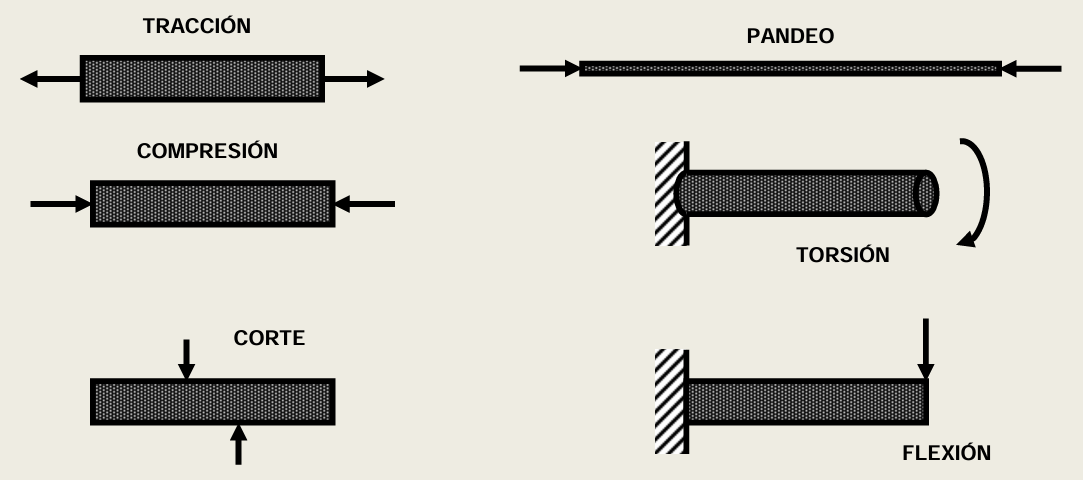
\includegraphics[width=0.7\textwidth]{Tipos_carga.png}
              \caption{Fuente: Transparencias Asignatura}
              \label{fig:tipos_carga}
          \end{figure}

    \item \textbf{Superficie y distribución de aplicación:} Carga concentrada (puntual), uniformemente distribuida o uniformemente variada.
          \begin{figure}[H]
              \centering
              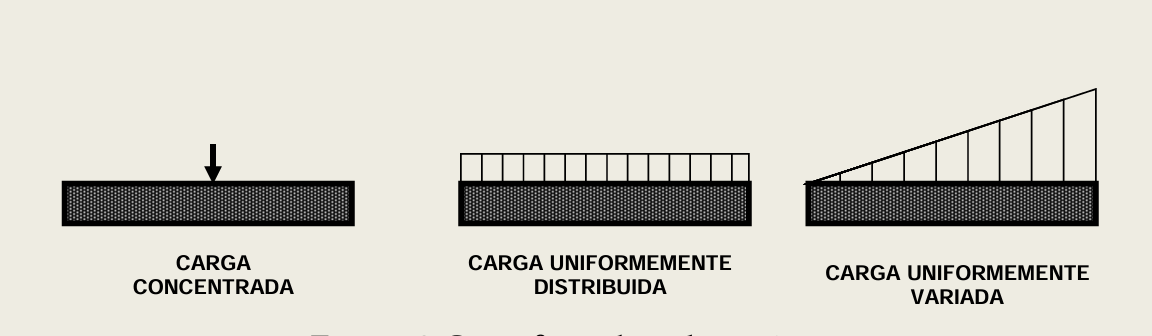
\includegraphics[width=0.7\textwidth]{superficie_aplicacion.png}
              \caption{Fuente: Transparencias Asignatura}
              \label{fig:superficie_aplicacion}
          \end{figure}
    \item \textbf{Tiempo y régimen de duración:}
          \begin{itemize}
              \item \textit{Carga constante o estática:} Aplicada de forma suave y mantenida en el tiempo.
              \item \textit{Carga progresiva:} Crecimiento lento y continuo de la solicitación.
              \item \textit{Carga repetitiva o cíclica:} Cargas variables en el tiempo que oscilan o fluctúan (origen de la fatiga).
              \item \textit{Carga alternativa:} Fluctuación completa del sentido de la carga (de $+P$ a $-P$).
              \item \textit{Carga de choque o impacto:} Aplicación brusca en fracciones de segundo con elevada transferencia de energía cinética.
          \end{itemize}
    \item \textbf{Condiciones del medio:} Temperatura de servicio (criogénica o elevada), exposición a atmósferas húmedas, salinas o fluidos corrosivos bajo tensión.
\end{enumerate}
\subsection{propiedades mecánicas}
El comportamiento mecánico de un material refleja la relación entre la fuerza aplicada y la respuesta del material a su deformación (resistencia que ofrece a la aplicación de la carga).
Las propiedades mecánicas de los materiales se determinan realizando ensayos normalizados que permiten comparar entre si el comportamiento de distintos materiales.
\begin{itemize}
    \item \textbf{Propiedades mecánicas de resistencia:} Comportamiento frente a esfuerzos axiales, cortantes o flectores (tracción, compresión, fatiga, termofluencia).
    \item \textbf{Propiedades mecánicas superficiales:} Resistencia a la deformación plástica localizada, penetración y rayado (dureza y resistencia al desgaste abrasivo).
    \item \textbf{Propiedades tecnológicas:} Capacidad del material para someterse a procesos de conformado y transformación (soldabilidad, flexión, embutición, abocardado).
\end{itemize}
Algunas normativas que lo regulan son ASME, ASTM y ISO.
\subsection{Conceptos Básicos de Elasticidad y Deformación}

\subsubsection{Tensión o Esfuerzo ($\sigma$)}
\dfn{Tensión o esfuerzo nominal}{Es la resistencia interna que ofrece una sección del material perpendicular a la carga aplicada. La tensión o esfuerzo que sufre un elemento ($\sigma$) es igual al cociente entre la fuerza uniaxial media y la sección transversal original de la barra.}

Considerando una barra o probeta prismática/cilíndrica de longitud inicial $l_0$ y sección transversal inicial $A_0$ sometida a una fuerza uniaxial normal $P$, la tensión $\sigma$ viene dada por:
\begin{equation}
    \sigma = \frac{P}{A_0}
    \label{eq:tension_nominal}
\end{equation}
\nt{La tensión ingenieriel siempre esta referida a la sección inicial}
\textbf{Unidades de tensión y esfuerzo habituales en ingeniería:}
\begin{itemize}
    \item \textbf{Sistema Internacional (SI):} Pascal ($\text{Pa} = \text{N}/\text{m}^2$). En ingeniería mecánica se emplean los múltiplos:
          \begin{equation*}
              1\text{ MPa} = 10^6\text{ Pa} = 1\text{ N}/\text{mm}^2, \qquad 1\text{ GPa} = 10^9\text{ Pa} = 10^3\text{ N}/\text{mm}^2
          \end{equation*}
    \item \textbf{Sistema Técnico:} Kilogramo-fuerza por centímetro cuadrado ($\text{kgf}/\text{cm}^2$) o por milímetro cuadrado ($\text{kgf}/\text{mm}^2$), donde $1\text{ kgf} \approx 9.80665\text{ N}$.
    \item \textbf{Sistema Anglosajón (U.S. Customary Units):} Libra-fuerza por pulgada cuadrada ($\text{psi} = \text{lbf}/\text{in}^2$) o miles de psi ($\text{ksi} = 10^3\text{ psi}$):
          \begin{equation*}
              1\text{ psi} \approx 6.89476 \times 10^3\text{ Pa}, \qquad 1\text{ ksi} \approx 6.89476\text{ MPa}
          \end{equation*}
\end{itemize}

\subsubsection{Deformación y Deformación Unitaria ($\varepsilon$)}
\dfn{Deformación}{Al aplicar una carga uniaxial $P$, el elemento experimenta una variación dimensional en la dirección longitudinal de la fuerza denominada alargamiento o deformación total $\delta = l - l_0$. Es decir es el incremento de la longitud de la barra o probeta inicial. }

\dfn{Deformación Unitaria}{En ingeniería se define la \textbf{deformación unitaria nominal} ($\varepsilon$) como el cociente entre el incremento de longitud y la longitud inicial de referencia:}
\begin{equation}
    \varepsilon = \frac{\delta}{l_0} = \frac{l - l_0}{l_0} \quad [\text{adimensional, habitualmente expresada en } \% \text{ o en } \text{mm}/\text{mm}]
    \label{eq:deformacion_unitaria}
\end{equation}

\subsubsection{Coeficiente de Poisson ($\nu$ o $\eta$)}
Una deformación longitudinal uniaxial viene invariablemente acompañada por una deformación transversal de sentido opuesto (contracción lateral en tracción, dilatación lateral en compresión). En materiales elásticos homogéneos e isótropos, las deformaciones unitarias transversales en los ejes perpendiculares son iguales ($\varepsilon_x = \varepsilon_y$).

El \textbf{coeficiente de Poisson} se define como el valor negativo del cociente entre la deformación unitaria lateral y la deformación unitaria longitudinal axial ($\varepsilon_z$):
\begin{equation}
    \nu = -\frac{\varepsilon_x}{\varepsilon_z} = -\frac{\varepsilon_y}{\varepsilon_z}
    \label{eq:poisson_ratio}
\end{equation}

Para un material idealmente incompresible bajo deformación elástica (sin variación de volumen), $\nu = 0.50$. En los materiales estructurales y metales de interés en ingeniería mecánica, $\nu$ oscila habitualmente entre $0.25$ y $0.40$ (Tabla~\ref{tab:poisson_valores}).

\begin{table}[H]
    \centering
    \begin{tabular}{lc lc}
        \toprule
        \textbf{Metal / Aleación} & \textbf{Coeficiente $\nu$} & \textbf{Metal / Aleación}     & \textbf{Coeficiente $\nu$} \\
        \midrule
        Aluminio                  & 0.33                       & Latón                         & 0.35                       \\
        Cobre                     & 0.35                       & Magnesio                      & 0.29                       \\
        Níquel                    & 0.31                       & Acero ordinario / estructural & 0.27 -- 0.30               \\
        Titanio                   & 0.36                       & Tungsteno (Wolframio)         & 0.28                       \\
        \bottomrule
    \end{tabular}
    \caption{Coeficientes de Poisson característicos para metales y aleaciones habituales.}
    \label{tab:poisson_valores}
\end{table}

\subsubsection{Deformación Elástica frente a Deformación Plástica}
Al someter a una fuerza de tensión uniaxial $\sigma$, el material sufre deformación, dependiendo de como quede el material despues de retirarla podemos hablar de:

\begin{itemize}
    \item \textbf{Deformación elástica:} Si al retirar la carga el material recupera instantáneamente sus dimensiones iniciales $l_0$.
    \item \textbf{Deformación plástica:} Si al retirar la carga el material experimenta una deformación permanente y residual. Durante esta deformación se ha producido una reorganización estructural del material y los atomos se han desplazado de sus posiciones de equilibrio.
\end{itemize}
\newpage
\section{Ensayo de Tracción}

El ensayo de tracción uniaxial es el procedimiento estándar más importante para determinar cuantitativamente las propiedades mecánicas de resistencia y deformabilidad de los materiales.

Se someten a un lento estiramiento mediante una equipo de ensayo \ref{fig:ensayo_traccion_esquema}, observándose la carga resultante y la deformación unitaria obtenida hasta el momento de la rotura final de la pieza. Debido a que las tensiones son monoaxiales y no poliaxiales tal y como se dan en la realidad
este ensayo \textbf{No proporciona conclusiones definitivas, Pero es clave para comparar diferentes materiales entre si, ademas las condiciones a las que se realiza el ensayo deben estar normalizadas} es decir se usan probetas de dimensiones establecidas, ademas de a una velocidad y temperatura prefijadas.

\begin{figure}[H]
    \centering
    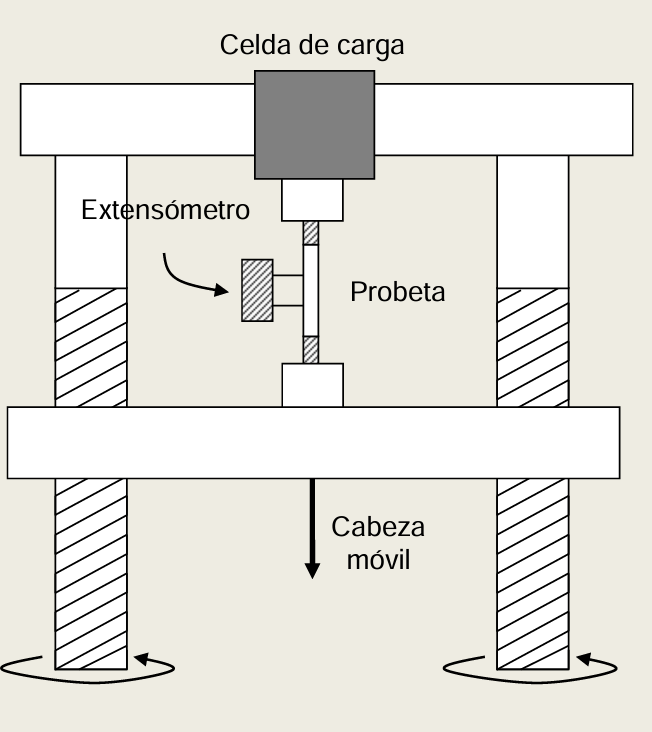
\includegraphics[width=0.7\textwidth]{ensayo_traccion.png}
    \caption{Esquema del ensayo de tracción.\\ Fuente: Transparencias Asignatura}
    \label{fig:ensayo_traccion_esquema}
\end{figure}

\subsection{Probetas Normalizadas (Norma ASTM)}
Para garantizar la reproducibilidad y comparación interlaboratorio, el ensayo se realiza bajo condiciones normalizadas (velocidad de deformación controlada y temperatura ambiente controlada). La Sociedad Americana de Ensayos de Materiales (\textbf{ASTM}) especifica geometrías estandarizadas:
\begin{itemize}
    \item \textbf{Probetas de sección circular:} Utilizadas comúnmente en piezas forjadas, barras y fundiciones. Presentan una longitud calibrada central reducida de diámetro $d_0 = 0.500'' \pm 0.010''$ ($12.7\text{ mm}$) y una longitud de calibración $L_0 = 2.000'' \pm 0.005''$ ($50.8\text{ mm}$). \textcolor{red}{En general, se exige la condición geométrica:} \nt{En caso de que la relación sea mayor}
          \begin{equation}
              \frac{L_0}{d_0} \leqslant 4
          \end{equation}
    \item \textbf{Probetas de sección rectangular:} Utilizadas para ensayos de chapas, perfiles y láminas laminadas, adaptando el espesor al del producto comercial y con transiciones curvas amplias hacia los cabezales de amarre.
\end{itemize}
Los extremos ensanchados de la probeta se sujetan mediante mordazas de cuña, asegurando que la rotura ocurra siempre en la zona central calibrada y no en las proximidades de las mordazas donde se generan concentraciones locales de tensiones.

\subsection{Curva Tensión-Deformación y Puntos Característicos}

Si se coloca la probeta en la máquina de ensayo de tracción y compresión y se aplica gradualmente \textbf{fuerzas de tracción} en los extremos, se puede medir \textbf{el alargamiento total en la longitud patrón para cualquier incremento predeterminado de la carga axial.} Las máquinas llevan generalmente un dispositivo que representa en un diagrama \textbf{la relación entre la carga (P) y el alargamiento ($\delta$).} Normalmente en los diagramas tensióndeformación se representa el \textbf{esfuerzo desarrollado en la probeta ($\sigma$) frente a la deformación unitaria ($\epsilon$)}

\begin{figure}[H]
    \centering
    \includegraphics[width=0.7\textwidth]{diagrama_tension_deformacion.png}
    \caption{Diagrama tensión-deformación para distintos materiales. Fuente: Transparencias Asignatura}
    \label{fig:diagrama_tension_deformacion}
\end{figure}
\begin{itemize}
    \item \textbf{Materiales dúctiles (a)} (ej. aceros de bajo carbono, cobre, aluminio recocido): Presentan un alargamiento elástico inicial lineal, una clara zona de deformación plástica uniforme generalizada, estricción localizada y un elevado alargamiento total antes de la fractura (Punto de rotura).
    \item \textbf{Materiales frágiles (b)} (ej. fundiciones grises, cerámicos, aceros de altísima dureza): Prácticamente no exhiben deformación plástica; la rotura se produce de manera repentina poco después de superado el régimen elástico lineal, con deformación a rotura insignificante.
    \item \textbf{Materiales elastoméricos / polímeros termoplásticos (c):} Muestran curvas no lineales con grandes deformaciones como se aprecia en la gráfica.
\end{itemize}
\nt{En el eje y siempre debe ir la tensión ingenieril es decir respecto a la sección inicial}
Del diagrama se pueden obtener una serie de puntos claves que caracterizan a los materiales como son:
\begin{multicols}{2}
    \begin{itemize}
        \item Límite de proporcionalidad elástico
        \item Límite elástico
        \item Puntos de fluencia
        \item Resistencia máxima a la tracción
        \item Punto de rotura
        \item Ductilidad
        \item Resiliencia
        \item Tenacidad
    \end{itemize}
\end{multicols}
\begin{figure}
    \centering
    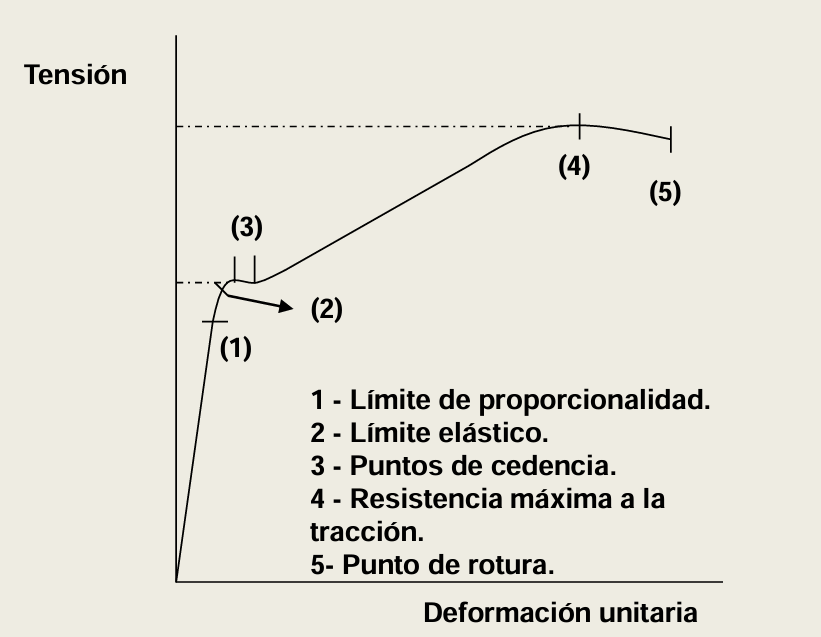
\includegraphics[width=0.7\textwidth]{puntos_diagrama_tension_deformacion.png}
    \caption{Puntos característicos de la curva tensión-deformación del acero.\\ Fuente: Transparencias Asignatura}
    \label{fig:puntos_diagrama_tension_deformacion}
\end{figure}
Estos puntos son importantes, ya que nos permiten determinar la tensión maxima para el diseño del equipo, aunque dependiendo del caso se optará por unos puntos u otros.
\subsubsection{Módulo de Young ($E$) y Límite de Proporcionalidad ($\sigma_{LP}$)}
Es la relacion entre la tensión $\sigma$ y la deformación $\varepsilon$, se calcula en el tramo inicial de la curva donde la relación es estrictamente proporcional cumpliéndose la \textbf{Ley de Hooke}:
\begin{equation}
    \sigma = E \, \varepsilon \quad \Longleftrightarrow \quad \frac{P}{A_0} = E \, \frac{\delta}{L_0}
    \label{eq:hooke_law}
\end{equation}
La constante de proporcionalidad $E$ se denomina \textbf{Módulo de Elasticidad o Módulo de Young}. Representa la rigidez del material frente a la deformación elástica:
\begin{itemize}
    \item Un valor elevado de $E$ indica un material rígido (requiere elevados esfuerzos para sufrir deformación elástica).
    \item Un valor bajo de $E$ describe un material flexible o elástico.
\end{itemize}

\begin{table}[H]
    \centering
    \begin{tabular}{lccc}
        \toprule
        \textbf{Material}                  & \textbf{$E$ ($\text{psi}$)} & \textbf{$E$ ($\text{GPa}$)} & \textbf{$E$ ($\text{Pa}$)} \\
        \midrule
        Cobre recocido                     & $16 \times 10^6$            & $110$                       & $1.1 \times 10^{11}$       \\
        Acero ordinario y de baja aleación & $29 \times 10^6$            & $200$                       & $2.0 \times 10^{11}$       \\
        Aleaciones de aluminio estructural & $10 \times 10^6$            & $70$                        & $0.7 \times 10^{11}$       \\
        Titanio comercial puro             & $15 \times 10^6$            & $105$                       & $1.05 \times 10^{11}$      \\
        \bottomrule
    \end{tabular}
    \caption{Módulos de Young característicos para distintos metales de uso en ingeniería.}
    \label{tab:modulos_young}
\end{table}

\dfn{Límite de proporcionalidad ($\sigma_{LP}$)}{El \textbf{límite de proporcionalidad} ($\sigma_{LP}$) representa el nivel máximo de tensión a partir del cual la relación lineal deja de cumplirse:}
\begin{equation}
    \sigma_{LP} = \frac{P_{LP}}{A_0}
\end{equation}
\imp{La tensión en el límite de proporcionalidad ($\sigma_{LP}$) es la correspondiente al punto donde deja de existir una relación lineal entre el esfuerzo aplicado y la deformación unitaria. $P_{LP}$ es la carga aplicada en el límite de proporcionalidad.}
\textbf{Método de Johnson para determinar $\sigma_{LP}$:} Dado que la desviación de la linealidad puede ser gradual y difícil de discernir visualmente, se emplea el método gráfico de Johnson: se traza una recta $OE$ tangente a la curva en el origen con pendiente $E$, y se define otra recta $OD$ con una pendiente un $50\%$ inferior respecto al eje de esfuerzos (es decir, en una paralela horizontal a distancia $FD = 1.5 \, FE$). Trazando una paralela a $OD$ que sea tangente a la curva de tracción, el punto de tangencia define con rigor el límite de proporcionalidad.
\begin{figure}[H]
    \centering
    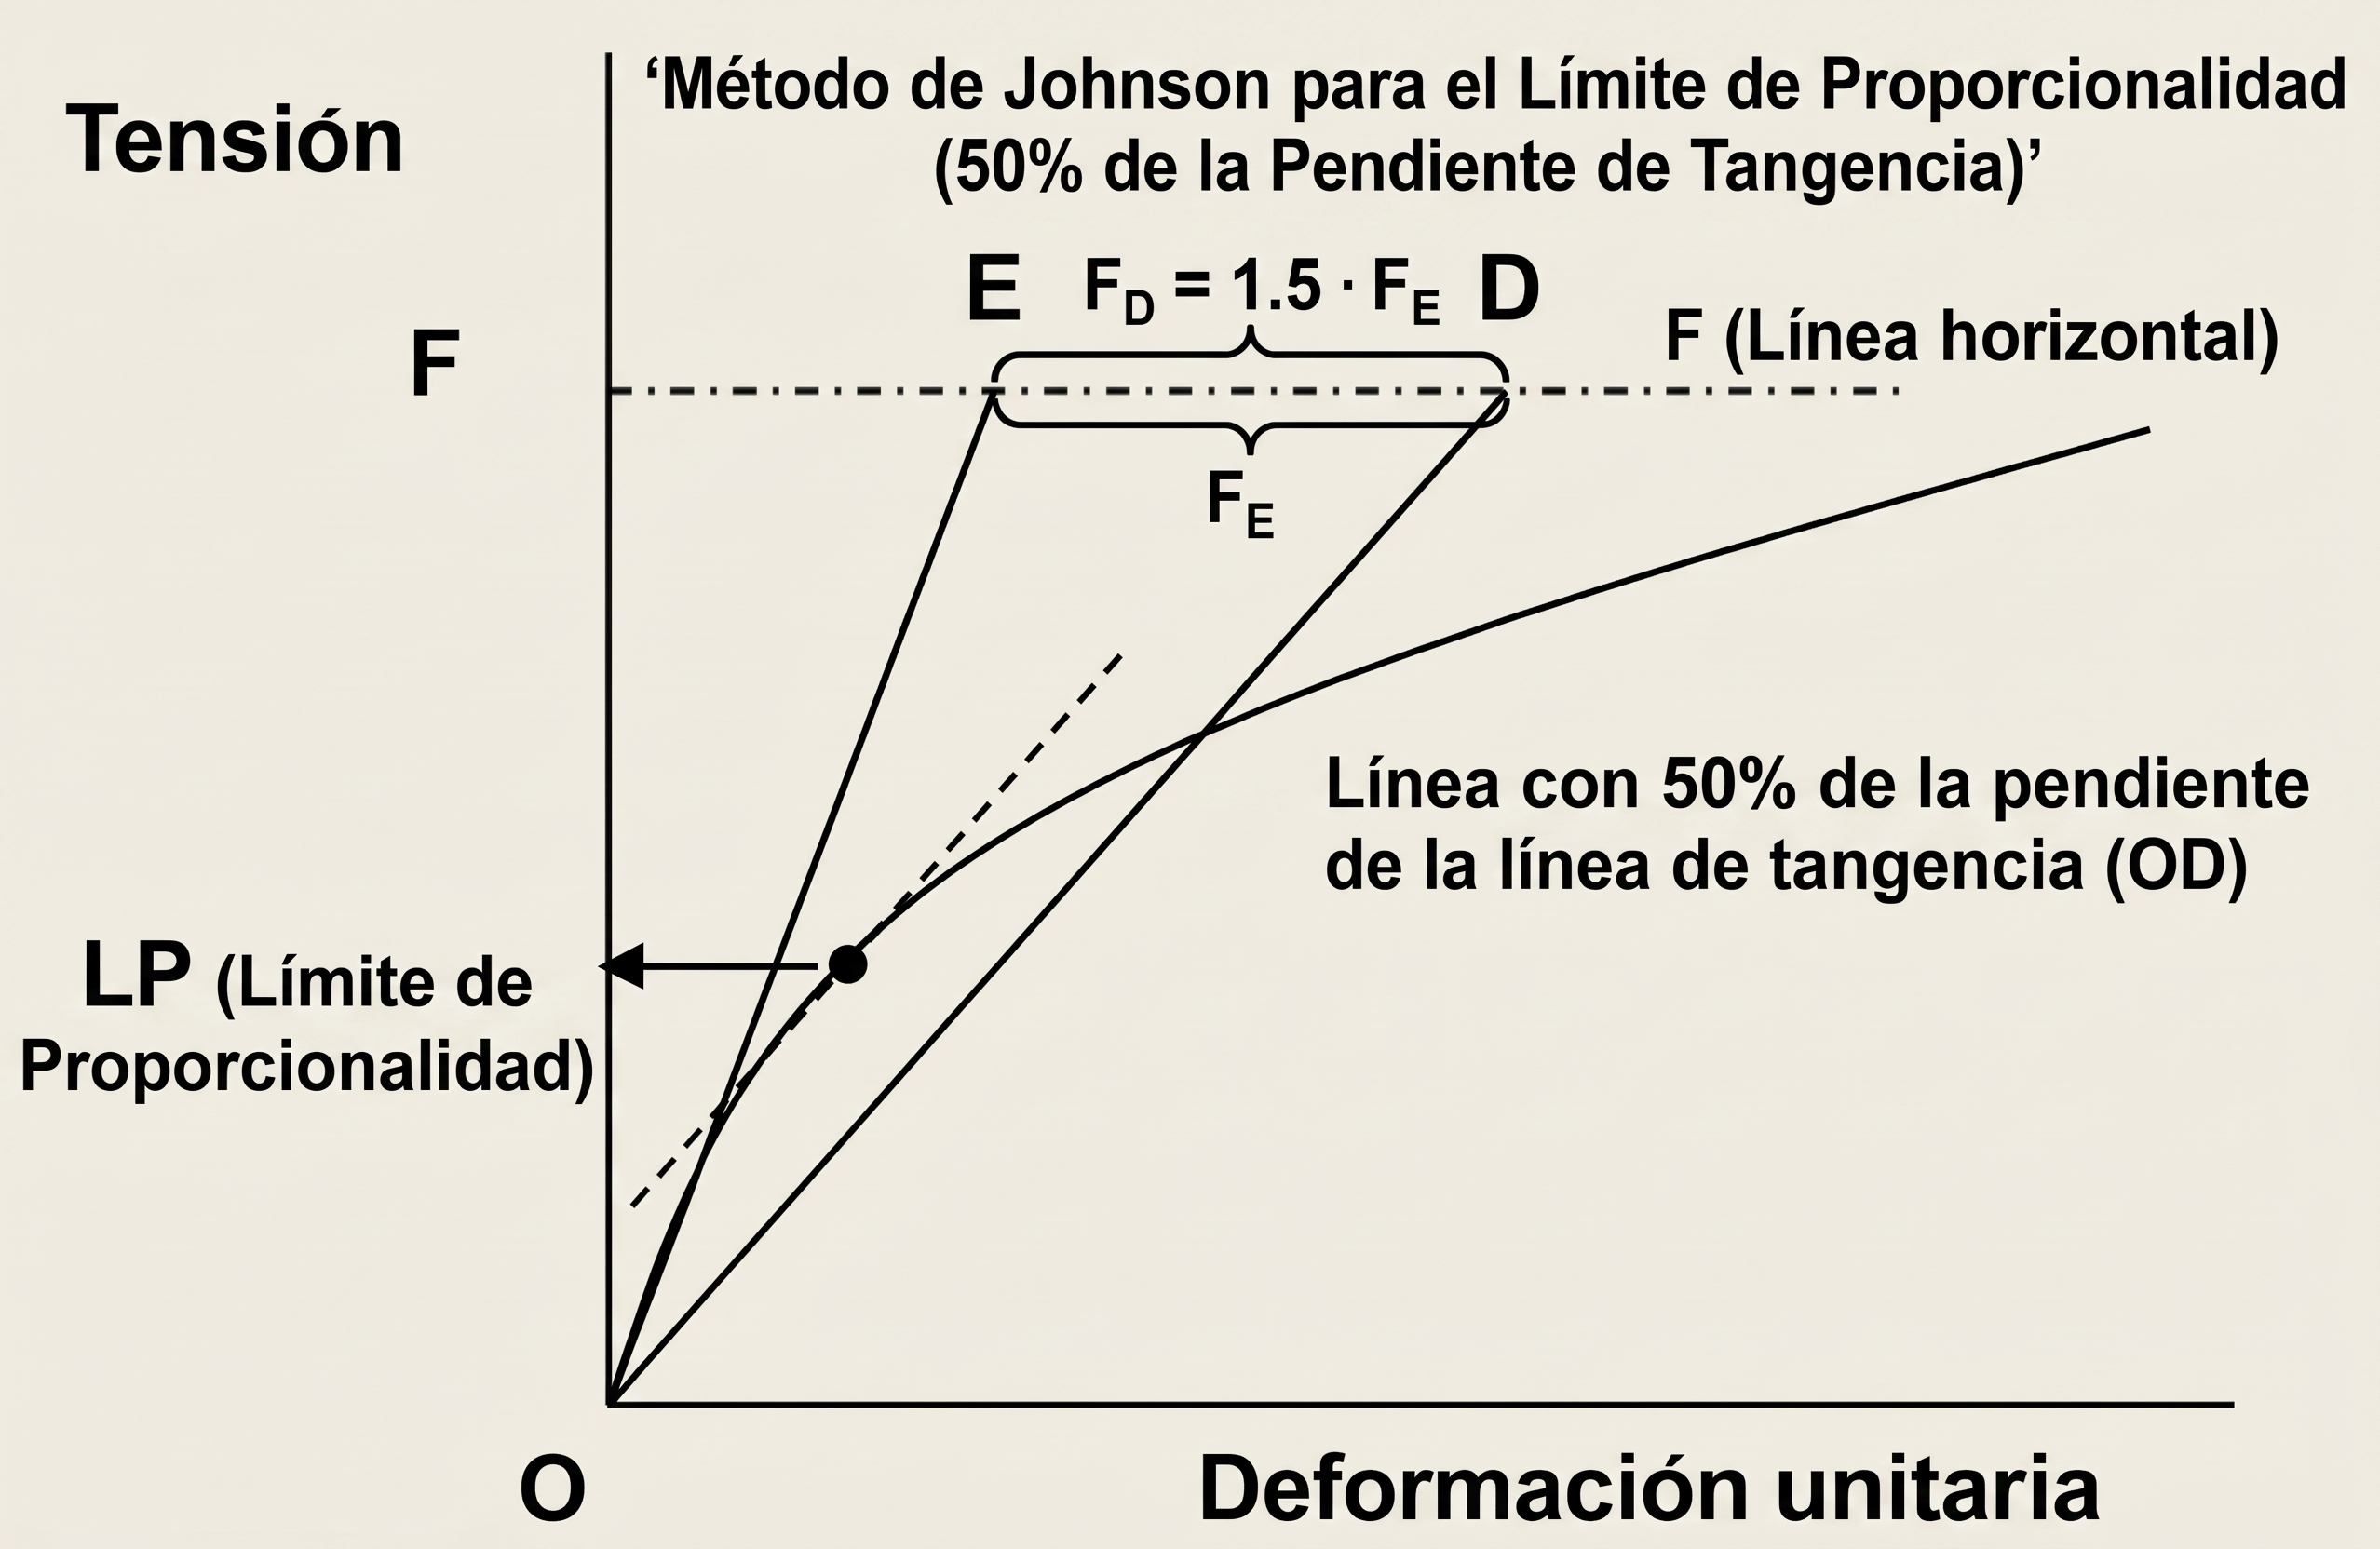
\includegraphics[width=0.7\textwidth]{Gemini_Generated_Image_a8mnpsa8mnpsa8mn.jpg}
    \caption{Método de Johnson para determinar $\sigma_{LP}$. Fuente: Transparencias Asignatura}
    \label{fig:metodo_johnson}
\end{figure}
\subsubsection{Límite de Elasticidad ($\sigma_{LE}$)}
Es la tensión máxima admisible sin que se produzcan deformaciones permanentes al cesar la carga. Generalmente coincide con el límite de proporcionalidad y se evalúa a partir de la siguiente expresión:
\begin{equation}
    \sigma_{LE} = \frac{P_{LE}}{A_0}
\end{equation}
donde \textbf{$P_{LE}$ es la carga aplicada en el límite de elasticidad.} Si al material ensayado se le aplica una carga superior sufrira una deformación plástica, por lo general se suele trabajar por debajo del limite de elasticidad (teniendo tambien en cuenta un coeficiente de seguridad).

\subsubsection{Límite o Punto de Fluencia / Cedencia ($\sigma_{LF}$ o $\sigma_A$)}
Es el valor de tensión a partir del cual el material experimenta un alargamiento considerable sin necesidad de aumentar la carga exterior.

Algunas veces la fluencia viene acompañada de un descenso en la tensión y en ese caso se aprecian dos puntos de fluencia:
\begin{itemize}
    \item \textbf{Punto de fluencia superior ($\sigma_{LFs} = P_A/A_0$):} \textbf{Depende de la forma con la que se realiza el ensayo}, es decir de la geometría de la probeta y de la velocidad de aplicación del ensayo.
    \item \textbf{Punto de fluencia inferior ($\sigma_{LFi} = P_B/A_0$):} \textbf{Es una propiedad intrínseca del material}, es decir es un punto característico del material.
\end{itemize}

\textbf{Convención de fluencia al 0.2\% ($\sigma_{0.2}$):} En aquellos materiales que no presentan un escalón de fluencia pronunciado (como los aceros de alta aleación, cobres, latones o aleaciones de aluminio), se define el límite elástico convencional como la tensión que genera una deformación plástica permanente remanente del $0.2\%$ ($\varepsilon = 0.002\text{ mm}/\text{mm}$). Se calcula trazando una recta paralela al tramo lineal elástico que parte desde la abscisa $\varepsilon = 0.002$; la intersección con la curva define el punto de fluencia de diseño.
\dfn{Tensión de fluencia sin límite definido obvio:}{Esfuerzo desarrollado en la probeta que provoca sobre el material una deformacion permanente del 0.2\%}
\subsubsection{Resistencia Máxima a la Tracción ($\sigma_M$ o $S_u$)}
Si se aumenta la carga aplicada sobre la probeta mas allá del punto de fluencia,es decir a medida que la probeta sigue deformándose plásticamente, experimenta endurecimiento por deformación hasta alcanzar la carga máxima admisible $P_M$. La resistencia última a la tracción referida a la sección inicial es:
\begin{equation}
    \sigma_M = \frac{P_M}{A_0}
\end{equation}
Una vez superado el punto de resistencia máxima, la deformación plástica deja de ser homogénea a lo largo de toda la longitud calibrada y se concentra en una zona restringida, originándose el fenómeno de \textbf{estricción} (formación de un cuello o garganta donde el área transversal real disminuye drásticamente). Debido a esta rápida reducción de área transversal, la carga global $P$ requerida para continuar el estiramiento decrece de forma aparente.
\nt{Correspone al punto M, que representa la resistencia máxima a tracción del material referida a la sección inicial de la probeta}
\newpage
\subsubsection{Punto y Tensión de Rotura ($\sigma_D$)}
Corresponde al punto final donde la probeta fractura definitivamente bajo una carga D.
\begin{figure}[H]
    \centering
    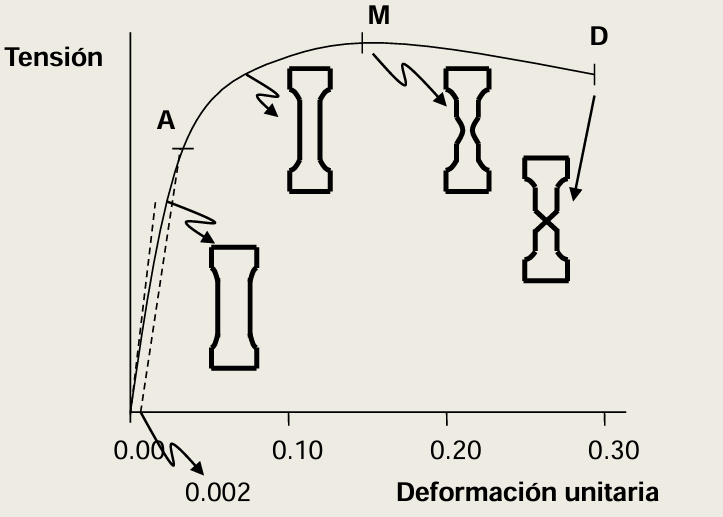
\includegraphics[width=0.7\textwidth]{punto_rotura.png}
    \caption{Resistencia máxima y punto de rotura \\ Fuente: Transparencias Asignatura}
    \label{fig:punto_rotura}
\end{figure}
\subsubsection{Ductilidad: Alargamiento y Estricción a la Rotura}
\dfn{Ductilidad:}{Grado de deformación plástica que puede soportar un material antes de su fractura.}
La ductilidad se determina cuantitativamente mediante el Alargamiento a la rotura (AR) y la Estricción a la rotura (ER) a partir de los datos obtenidos tras un ensayo de tracción con las siguientes expresiones:
\begin{enumerate}
    \item \textbf{Porcentaje de alargamiento a la rotura (\%AR):}
          \begin{equation}
              \%AR = \frac{l_f - l_0}{l_0} \times 100
              \label{eq:porcentaje_ar}
          \end{equation}
    \item \textbf{Porcentaje de estricción (\%ES):}
          \begin{equation}
              \%ES = \frac{A_0 - A_f}{A_0} \times 100
              \label{eq:porcentaje_es}
          \end{equation}
\end{enumerate}
donde $l_0$ y $A_0$ son la longitud calibrada y la sección inicial, y $l_f$ y $A_f$ son la longitud final entre puntos calibrados y la sección transversal mínima en el cuello de rotura.
\nt{A mayores valores de \%AR y \%ES, mayor es la ductilidad del material y su seguridad frente a roturas catastróficas.}
\begin{itemize}
    \item \textbf{Material frágil:} aquel que no puede tener apenas deformación plástica antes de romperse, se rompen de golpe, sin avisar. Por ejemplo el vidrio. Los materiales frágiles son aquellos que no han sufrido deformación plástica antes de romperse (se rompen justo en el límite elástico).
    \item \textbf{Material dúctil:} aquel que puede tener grandes deformaciones plásticas antes de romperse
\end{itemize}
\subsubsection{Resiliencia y Módulo de Resiliencia}
\dfn{Resiliencia:}{Es la capacidad de un material de absorber energía elástica cuando es deformado y devolverla íntegramente al retirar la carga exterior.}
\nt{Representa el área bajo el tramo elástico de la curva tensión-deformación hasta el límite de proporcionalidad.}

La energía de deformación elástica acumulada en el volumen de la probeta es el trabajo desarrollado por la fuerza:
\begin{equation}
    U = \frac{1}{2} P_{LP} \, \delta_{LP} \quad \xRightarrow{\text{Con la def. de }\sigma_{LP} \text{ y la ley de Hooke}} \frac{1}{2} \left(\frac{\sigma_{LP}^2}{E}\right) A_0 \, L_0
\end{equation}
El \textbf{Módulo de Resiliencia} ($U_r$) se define como la energía elástica absorbida por unidad de volumen de material:
\begin{equation}
    U_r = \frac{U}{A_0 \, L_0} = \frac{1}{2} \, \frac{\sigma_{LP}^2}{E}
    \label{eq:modulo_resiliencia}
\end{equation}
\textbf{Esta propiedad cuantifica la resistencia frente a choques a baja velocidad} y para maximizarla se requieren materiales con elevado límite elástico $\sigma_{LP}$ y bajo módulo elástico $E$.

\subsubsection{Tenacidad y Ensayos de Impacto (Charpy e Izod)}
\dfn{Tenacidad:}{Es la capacidad de un material de absorber energía mecánica elástica y plástica antes de que se produzca la fractura.}
Representa la energía máxima absorbida por unidad de volumen antes de originarse la ruptura total del material, se puede obtener de las siguientes formas:
\begin{itemize}
    \item Corresponde al área total bajo la curva completa tensión-deformación hasta el punto de rotura. Puede estimarse analíticamente de forma aproximada mediante la regla del trapecio:
          \begin{equation}
              \text{Tenacidad} \approx \frac{\sigma_A + \sigma_M}{2} \cdot \delta_D
              \label{eq:tenacidad_aprox}
          \end{equation}
          donde $\sigma_A$ es la tensión de fluencia, $\sigma_M$ la resistencia última y $\delta_D$ la deformación total a rotura.
    \item Evaluada mediante \textbf{ensayos normalizados de impacto en probetas entalladas (ensayos Charpy e Izod)}. Un martillo pendular de masa conocida se libera desde una altura inicial $h$, fractura la probeta entallada por flexión en un único golpe y asciende hasta una altura residual $h' < h$. La energía absorbida en el impacto es:
          \begin{equation}
              E_{\text{impacto}} = m g (h - h')
          \end{equation}
          \begin{itemize}
              \item \textit{Ensayo Charpy:} La probeta se apoya como viga simplemente apoyada en ambos extremos y el péndulo golpea en el centro por la cara opuesta a la entalla. Se utiliza típicamente en materiales dúctiles y aceros estructurales.
              \item \textit{Ensayo Izod:} La probeta se empotra verticalmente en voladizo y el péndulo golpea a una distancia fija en la cara donde se ubica la entalla. Muy empleado para plásticos y materiales más frágiles.
          \end{itemize}
\end{itemize}
\imp{La diferencia entre ambos ensayos es la forma de colocar la probeta. El ensayo de Izod se utiliza para determinar la tenacidad en materiales frágiles y el de Charpy para materiales dúctiles, ademas los resultados de los ensayos son cualitativos y se realizan con fines comparativos.}
\begin{figure}[H]
    \centering
    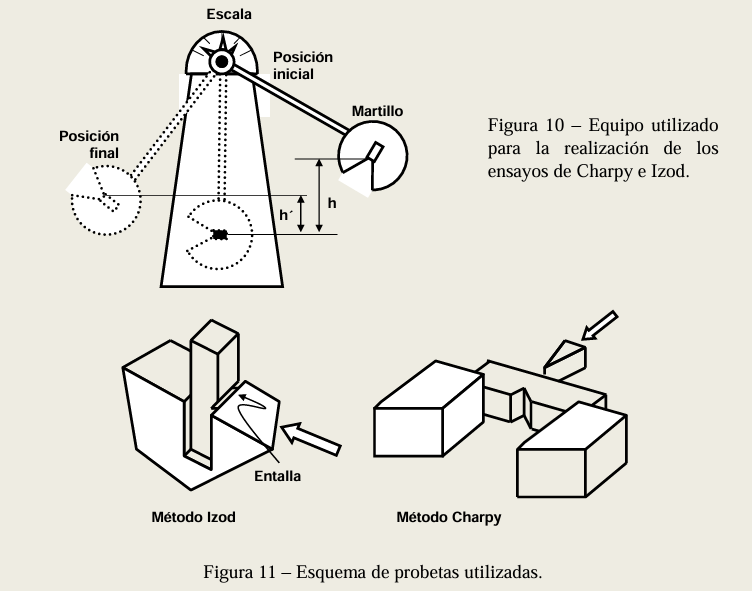
\includegraphics[width=0.6\textwidth]{ensayo_charpy_e_izod.png}
    \caption{Esquema del ensayo de \textbf{Charpy e Izod} \\ Fuente: Transparencias Asignatura}
    \label{fig:ensayo_charpy_e_izod}
\end{figure}
\paragraph{Transición Dúctil-Frágil y Efecto de la Temperatura:}
En metales con estructura cristalina cúbica centrada en el cuerpo (\textbf{BCC}, como los aceros al carbono ferríticos), la energía absorbida cae drásticamente al disminuir la temperatura, pasando de un comportamiento dúctil a alta absorción de energía a una rotura frágil y quebradiza por exfoliación a bajas temperaturas. Por el contrario, los metales con estructura cúbica centrada en las caras (\textbf{FCC}, como los aceros inoxidables austeníticos, aluminio, cobre y níquel) no presentan una transición brusca y retienen excelente tenacidad incluso a temperaturas criogénicas.

Asimismo, el contenido de carbono afecta de forma acusada: a medida que aumenta el porcentaje de carbono en los aceros recocidos, el material se vuelve más frágil, absorbe menos energía en el ensayo Charpy y el rango de transición hacia la fragilidad se desplaza a temperaturas más elevadas.
\imp{Es decir, en estos ensayos es importante la temperatura ya que puede haber una transición de ductil a fragil (cuando desciende la temperatura), ademas si cambiamos el contenido en carbono de los aceros recocidos se vuelven mas quebradizos y son capaces de absorber menos energía antes de su rotura.}
\begin{figure}[H]
    \centering
    \begin{subfigure}[c]{0.67\textwidth}
        \centering
        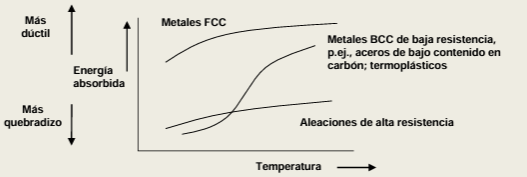
\includegraphics[height=4.2cm]{ductil_temperatura.png}
        \caption{Efecto de la temperatura en la tenacidad}
        \label{fig:ductil_temperatura}
    \end{subfigure}
    \hfill
    \begin{subfigure}[c]{0.3\textwidth}
        \centering
        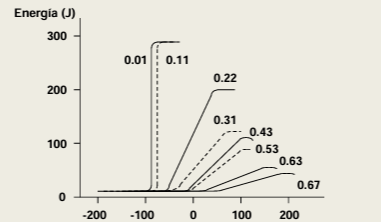
\includegraphics[height=4.2cm]{ductil_composicion.png}
        \caption{Efecto del porcentaje de carbono}
        \label{fig:ductil_composicion}
    \end{subfigure}
    \caption{Factores que influyen en la transición dúctil-frágil}
    \label{fig:ductil_transicion}
\end{figure}

\subsection{Tensiones y Deformaciones Reales}
En el cálculo convencional de ingeniería se utilizan el esfuerzo ingenieril $\sigma = P/A_0$ y la deformación ingenieril $\varepsilon = \delta/L_0$, es decir, se asume la sección inicial transversal a la aplicación de la carga para todos los calculos. Esto genera la falsa apariencia gráfica de que, superada la resistencia máxima, el material resiste menos esfuerzo. En la realidad física, el área transversal instantánea $A_i$ en la zona de estricción disminuye mucho más rápido que la carga aplicada, de modo que la tensión verdadera que soporta el material, \textbf{aumenta monótonamente hasta la rotura.}
\begin{figure}[H]
    \centering
    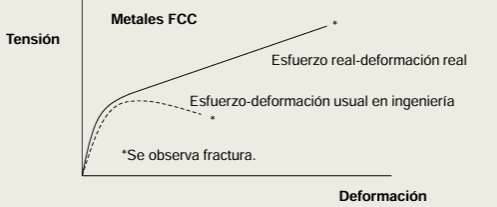
\includegraphics[width=0.7\textwidth]{deformacion_real.png}
    \caption{Tensión real vs Tensión ingenieril \\ Fuente: Transparencias Asignatura}
    \label{fig:deformacion_real}
\end{figure}
Se definen la \textbf{tensión real} ($\sigma_T$) y la \textbf{deformación real logarítmica} ($\varepsilon_T$) como:
\begin{equation}
    \sigma_T = \frac{P}{A_i}, \qquad \varepsilon_T = \int_{l_0}^{l_i} \frac{dl}{l} = \ln\left(\frac{l_i}{l_0}\right)
    \label{eq:tension_deformacion_reales}
\end{equation}
Asumiendo constancia de volumen durante la deformación plástica ($A_0 l_0 = A_i l_i$), se obtienen las relaciones de conversión válidas \textbf{hasta el comienzo de la estricción}:
\begin{equation}
    \sigma_T = \sigma \, (1 + \varepsilon), \qquad \varepsilon_T = \ln(1 + \varepsilon)
    \label{eq:conversion_real_nominal}
\end{equation}
\nt{Es decir que la tensión y deformación real estan relacionadas con las nominales(engenieriles) hasta que la probeta comienza a sufrir estricción.}
\paragraph{Ecuación constitutiva de Hollomon:}
En muchos metales y aleaciones, la región plástica comprendida entre el límite de fluencia y el comienzo de la estricción se ajusta fielmente a la ley potencial:
\begin{equation}
    \sigma_T = K \, \varepsilon_T^n
    \label{eq:hollomon}
\end{equation}
donde $K$ es el coeficiente de resistencia del material y $n$ es el \textbf{exponente de endurecimiento por deformación} ($n < 1$). A mayor valor de $n$, mayor es la capacidad del material para deformarse plásticamente de forma uniforme antes de que comience a localizarse la estricción (Tabla~\ref{tab:constantes_hollomon}).

\begin{table}[H]
    \centering
    \begin{tabular}{lcc}
        \toprule
        \textbf{Material}                     & \textbf{Exponente $n$} & \textbf{Constante $K$ ($\text{MPa}$)} \\
        \midrule
        Acero bajo en carbono (recocido)      & 0.26                   & 530                                   \\
        Acero aleado AISI 4340 (recocido)     & 0.15                   & 640                                   \\
        Acero inoxidable austenítico AISI 304 & 0.45                   & 1275                                  \\
        Aluminio recocido                     & 0.20                   & 180                                   \\
        Cobre recocido                        & 0.54                   & 315                                   \\
        Latón 70Cu-30Zn (recocido)            & 0.49                   & 895                                   \\
        Aleación de aluminio 2024-T4          & 0.16                   & 690                                   \\
        \bottomrule
    \end{tabular}
    \caption{Parámetros de endurecimiento por deformación ($n$ y $K$) para diversos materiales.}
    \label{tab:constantes_hollomon}
\end{table}

\subsection{Endurecimiento por Deformación Plástica (Acritud)}
Cuando un metal dúctil se somete a deformación plástica en frío (por encima de su límite elástico), la densidad de dislocaciones en su red cristalina se incrementa enormemente, multiplicándose y entorpeciendo su propio movimiento. \textbf{Es decir sufre una deformación plastica que produce un incremento de la resistencia elástica, tambien disminuye su ductilidad y aumenta su punto de fluencia.}

Si durante un ensayo de tracción se interrumpe la carga tras alcanzar una deformación plástica y se descarga el espécimen, el material desciende con una pendiente idéntica a la elástica ($E$). Al volver a aplicar carga, el material recorre el mismo camino elástico hasta alcanzar un \textbf{nuevo límite de fluencia significativamente más elevado} que el original.
\begin{figure}[H]
    \centering
    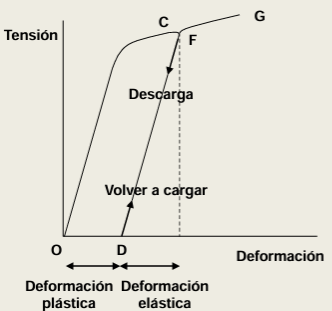
\includegraphics[width=0.5\textwidth]{endurecimiento_por_deformacion.png}
    \caption{Endurecimiento por deformación \\ Fuente: Transparencias Asignatura}
    \label{fig:endurecimiento_por_deformacion}
\end{figure}
\nt{En este grafico se observa como se le aplica una tensión inicial hasta recorriendo desde O hasta C, luego se descarga siguiendo la linea CD ya que al haber sufrido una deformación plastica no puede volver al estado original, siguiendo la trayectoria CD, al aplicar otra vez tensión seguira la trayectoria DF, siguiendo la ley de hooke hasta llegar a F y posteriormente si se sigue tensando habra un cambio brusco hasta G donde rompera.}
Este fenómeno confiere al material:
\begin{itemize}
    \item \textbf{Mayor rigidez y tensión elástica de servicio:} Se pueden aplicar cargas más altas sin que se genere nueva deformación plástica.
    \item \textbf{Aumento de la resistencia mecánica:} mejora unidireccional hacia donde se le aplico la carga, pero no mejora en el resto de las direcciónes del espacio.
    \item \textbf{Disminución de la ductilidad y de la tenacidad:} El material se torna más quebradizo.
    \item \textbf{Incremento del limite de proporcionalidad:} Aumenta la tensión necesaria para que el material comience a deformarse plásticamente.
    \item \textbf{Anisotropía:} El incremento de resistencia se produce preferentemente en la dirección en la que se aplicó la deformación uniaxial, pero no en las direcciones transversales.
    \item \textbf{Mayor susceptibilidad a la corrosión:} Las zonas con deformación plástica concentran tensiones residuales internas que aceleran la corrosión bajo tensión (aparece fluencia en las zonas no deformadas plásticamente).
\end{itemize}
El endurecimiento por deformación se puede revertir completamente restituyendo la ductilidad inicial mediante un \textbf{tratamiento térmico de recocido} a temperatura adecuada (tratamiento térmico suave a 100°C y posteriormente dejar enfriar lentamente).
\nt{Este tipo de tratamiento es común en procesos como el laminado de barras, estirado de tubos, ya que muchas veces se usa un material pretensado, es decir, se ha endurecido por acritud como se ha descrito previamente, un ejemplo sería en los pilares de hormigón pretensado, los cuáles son sometidos a esfuerzos de tracción para que se vuelvan más resistentes en dirección hacia donde sufrio la carga, aunque esto tiene un mayor coste economico.}
\section{Ensayo de Termofluencia (\textit{Creep})}

Muchos equipos de instalaciones químicas (\textbf{Reactores,turbinas}, calderas, intercambiadores de calor, columnas de destilación a presión y álabes de turbinas) operan simultáneamente bajo elevados esfuerzos mecánicos y altas temperaturas. A temperaturas elevadas las propiedades de los materiales experimentan cambios drásticos:
\begin{itemize}
    \item El módulo de elasticidad $E$ disminuye paulatinamente.
    \item El límite de proporcionalidad y la resistencia máxima a la tracción caen de forma notable a partir de cierta temperatura crítica.
    \item La ductilidad (\%AR y \%ES) se incrementa de forma acusada.
\end{itemize}

En estos equipos al sufrir una variación de temperatura importante, y tambien variación de presión (en especial en los reactores químicos de alta presión) las propiedades de los materiales pueden cambiar drásticamente, por lo que es importante conocer su comportamiento con este ensayo.

\subsection{Ensayo de tensión-deformación a distintas temperaturas}
\begin{figure}[H]
    \centering
    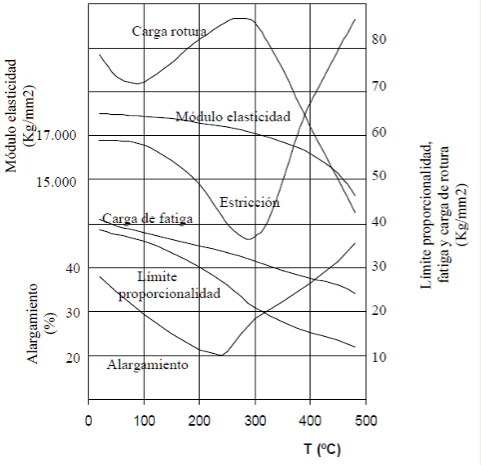
\includegraphics[width=0.5\textwidth]{termofluencia.png}
    \caption{Curva típica de termofluencia}
    \label{fig:termofluencia}
\end{figure}
En esta gráfica se puede observar la variación de las propiedades con la temperatura:
\begin{itemize}
    \item \textbf{Resistencia máxima a la tracción:} Crece hasta los 250\,°C.
    \item \textbf{Módulo de elasticidad:} Disminuye paulatinamente conforme aumenta la temperatura.
    \item \textbf{Contracción superficial (estricción):} Pasa por un mínimo a los 250\,°C y posteriormente crece de forma rápida.
    \item \textbf{Carga de fatiga:} Disminuye con la temperatura.
    \item \textbf{Límite de proporcionalidad:} Disminuye continuamente.
    \item \textbf{Alargamiento a la rotura:} Sigue un camino paralelo a la estricción ya que ambos definen la ductilidad (aumentan con la temperatura).
\end{itemize}

Los resultados de este ensayo arrojan la siguiente información:
\begin{itemize}
    \item Aquellas \textbf{propiedades que definen la ductilidad, como son la estricción y el alargamiento a la rotura, aumentan con la temperatura}
    \item las \textbf{propiedades relacionadas con la rigidez del material, como el límite de proporcionalidad y el módulo de elasticidad, disminuyen. La resistencia máxima a la tracción disminuye de forma apreciable tras una temperatura en específica}
\end{itemize}

\nt{En este gráfico se puede observar como la \textbf{resistencia a la tracción}} aumenta hasta los 250\,°C, mientras que el \textbf{módulo de elasticidad} disminuye de forma apreciable tras los 250\,°C, cabe mencionar que las \textbf{propiedades que definen la ductilidad, como son la estricción y el alargamiento a la rotura, aumentan con la temperatura}. Finalmente la \textbf{carga de fatiga} disminuye tras los 250\,°C.

Es importante considerar el tiempo como variable, ya que este ensayo es valido siempre y cuando  la carga actue durante un corto periódo de tiempo, si aumenta la duración (dias/semanas/meses) la carga necesaria para producir la rotura del material es cada vez mas pequeña.

\imp{para cargas que van a actuar durante largos períodos de tiempo y a temperaturas elevadas se necesitará una información más completa obtenida a partir de los ensayos termofluencia.}

\subsection{Ensayo de Termofluencia}
Bajo estas condiciones, la \textbf{variable tiempo} adquiere una importancia crítica. \textbf{Una pieza sometida a un esfuerzo constante inferior a su límite elástico puede sufrir una deformación plástica durante un cierto periodo de tiempo, esta deformación que depende del tiempo es conocida como termofluencia o fluencia lenta (\textit{creep})}.

\subsection{Curva Típica de Termofluencia y sus Etapas}
En un \textbf{ensayo} normalizado de \textbf{termofluencia}, una probeta se mantiene bajo \textbf{temperatura} rigurosamente controlada y \textbf{tensión} mecánica \textbf{constante}, registrando la \textbf{deformación en función del tiempo}. La curva característica presenta tres etapas bien diferenciadas:
\begin{enumerate}
    \item \textbf{Deformación elástica instantánea:} Es una deformación elástica instantánea que ocurre en el momento de aplicar la carga.
    \item \textbf{Etapa primaria o transitoria:} La probeta experimenta una deformación que aumenta progresivamente con el tiempo. el metal se endurece para soportar la carga aplicada por deformación, decreciendo la rapidez de la termofluencia con el tiempo a medida que el endurecimiento por deformación se hace más elevado.
    \item \textbf{Etapa secundaria o estacionaria:} La velocidad de deformación se mantiene prácticamente constante y mínima ($d\varepsilon/dt = \text{cte}$). En esta fase se establece un equilibrio dinámico entre el endurecimiento por deformación y los procesos térmicos de restauración y aniquilación de dislocaciones móviles promovidos por la difusión atómica. Tanto que el metal continúa alargandose a una velocidad constante, \textbf{La pendiente de esta región se denomina mínima rapidez de termofluencia}.
    \item \textbf{Etapa terciaria:} La velocidad de deformación se acelera de manera exponencial debido a la aparición de estricción macroscópica y la nucleación de microcavidades y grietas en los límites de grano, conduciendo rápidamente a la fractura del componente.
\end{enumerate}

la forma de la curva depende estrechamente de la carga y temperatura aplicada, Si existen esfuerzos y temperaturas elevadas, el tiempo necesario para la fractura del material disminuye de forma considerable.
\nt{Existen dos fenómenos importantes durante este proceso, un \textbf{endurecimiento del material provocado por la deformación plástica y un reblandecimiento causado al estar sometido a temperaturas elevadas.}}
\begin{figure}[H]
    \centering
    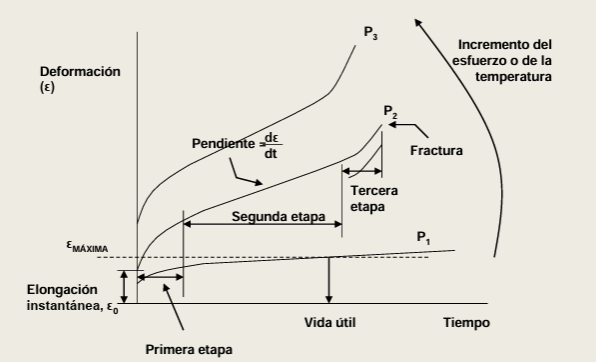
\includegraphics[width=0.7\textwidth]{ensayo_termofluencia.png}
    \caption{Curva típica de termofluencia}
    \label{fig:ensayo_termofluencia}
\end{figure}
Este ensayo se hace para materiales que soportaran altas temperaturas y cargas, como una turbina un reactor\dots
\imp{\textbf{La pendiente de la segunda etapa de la curva de termofluencia} es una medida que permite la comparación de diferentes materiales sometidos a las mismas condiciones del ensayo. El valor menor de la mínima rapidez de termofluencia una menor velocidad de deformación en esas condiciones.}
\nt{El esfuerzo que produce una \textbf{mínima rapidez de termofluencia de $10^{-5}\%/\text{h}$} también es otro parámetro que puede determinar la resistencia a la termofluencia e indicaría la evaluación de la carga máxima a aplicar al material a una determinada temperatura para que su velocidad de deformación fuese pequeña. \textbf{La elección de un material para trabajar a esfuerzo y temperaturas elevadas necesita de la realización de ensayos de termofluencia.} Este ensayo, junto con la \textbf{vida útil} del elemento, permite determinar fácilmente la \textbf{carga máxima} que puede ser aplicada sobre el material}
\section{Ensayo de Fatiga}

La \textbf{fatiga} es un mecanismo de degradación y \textbf{rotura} progresiva que se produce en piezas y componentes sometidos a tensiones dinámicas repetitivas, cíclicas o fluctuantes, por lo que el material falla con tensiones mucho mas pequeñas de las que podria soportar el material cuando se somete a cargas de tracción. \textbf{Es la primera causa de rotura de los materiales}

\textbf{Relevancia en ingeniería:} Representa la causa de más del $90\%$ de los fallos mecánicos en servicio en componentes metálicos. Lo más peligroso de la fatiga es que \textbf{la rotura sobreviene a tensiones notablemente inferiores a la resistencia estática de tracción e incluso por debajo del límite elástico, ocurriendo de forma súbita y sin deformación plástica previa apreciable}.

Las cargas aplicadas que producen fatiga pueden ser de distinta naturaleza: tracción, compresión, flexión o de naturaleza torsional. La resistencia que un material ofrece a la fatiga puede ser evaluada a partir de ensayos realizados en el laboratorio. Para ello la probeta se somete a esfuerzos alternativos de tracción y compresión de igual magnitud mediante el giro que provoca el equipo esquematizado, ademas las probetas son normalizadas. siguiendo el siguiente esquema
\nt{Suele ocurrir en equipos sometidos a presiones elevadas y tambien en ambientes corrosivos, otro ejemplo seria en un deposito donde se vacie y se llene continuamente.}
\subsection{Máquina de Ensayo y Curvas $S-N$ (Curvas de Wöhler)}
La resistencia a la fatiga se determina mediante ensayos dinámicos como el ensayo de flexión rotativa (máquina R.R.~Moore), en el que una probeta de sección calibrada gira a alta velocidad sometiéndose simultáneamente a tracción y compresión alternadas ($\sigma_{\text{med}} = 0$).

\begin{figure}
    \centering
    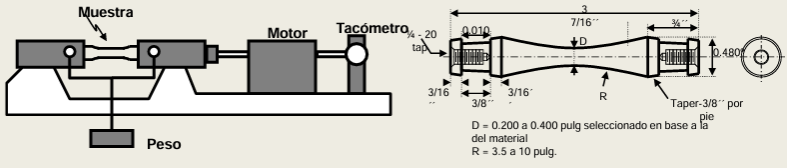
\includegraphics[width=0.7\textwidth]{ensayo_fatiga.png}
    \caption{Curva típica de fatiga}
    \label{fig:ensayo_fatiga}
\end{figure}

Los resultados se representan en un diagrama semilogarítmico de amplitud de tensión ($S$) frente al logaritmo del número de ciclos hasta la rotura ($N$):
\begin{itemize}
    \item \textbf{Materiales con límite de fatiga definido} (aceros al carbono y aleaciones de titanio): La curva $S-N$ se hace asintótica y totalmente horizontal a partir de un valor elevado de ciclos. Dicha asíntota define el \textbf{límite de fatiga} ($\sigma_e$ o $S_e$), que representa el nivel de tensión por debajo del cual el componente puede soportar un número infinito de ciclos sin romperse.
    \item \textbf{Materiales sin límite de fatiga definido} (aleaciones no férreas de aluminio, cobre, magnesio): La curva $S-N$ continúa descendiendo monótonamente. En este caso se define la \textbf{resistencia a la fatiga} para una vida prefijada de $N = 10^6$.
\end{itemize}

\begin{figure}
    \centering
    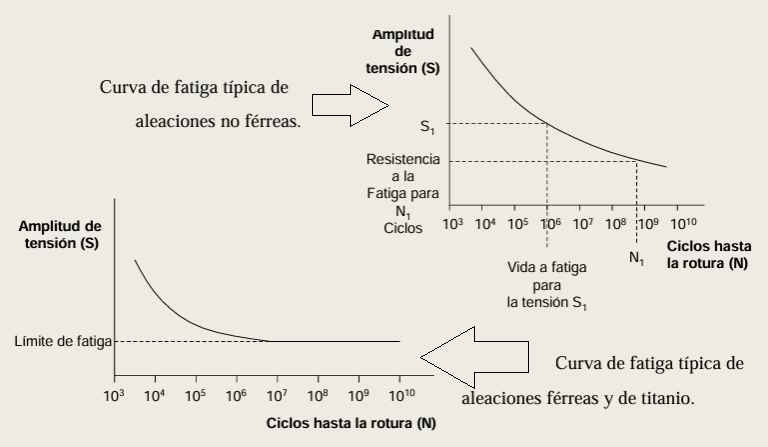
\includegraphics[width=0.7\textwidth]{curvas_fatiga.png}
    \caption{Curvas de fatiga para aleaciones ferricas y no ferricas. \\ Fuente: Callister, W. D. (2003). *Ciencia e Ingeniería de Materiales*. Grupo Editorial Iberoamericana.}
    \label{fig:curvas_fatiga}
\end{figure}
\imp{En resumen, los aceros al carbono y las aleaciones de titanio apresentam un límite de fatiga como la tensión para la cual el material puede someterse a infinitos ciclos. Otras aleaciones no férreas no presentan un límite de fatiga definido y para estos casos se define como la tensión de fatiga para la cual el material puede resistir hasta $10^6$ ciclos}
\subsection{Factores Críticos que Reducen la Vida a Fatiga}
La rotura por fatiga se inicia siempre en la superficie exterior y se propaga lentamente mediante microfisuras hasta la sección crítica restante. Los factores más determinantes son:
\begin{itemize}
    \item \textbf{Concentración de esfuerzos:} Entallas, ranuras, esquinas vivas, agujeros de paso o cambios bruscos de sección multiplican localmente las tensiones y actúan como iniciadores de grietas.
    \item \textbf{Rugosidad superficial:} Cuanto más pulida sea la superficie, mayor es la vida a fatiga; superficies rugosas o rayadas actúan como microentallas, cuanto mas pulido este el material el area superficial sera menor, y por tanto es menos susceptible a la corrosión y finalmente a la fatiga.
    \item \textbf{Ambiente de trabajo (fatiga-corrosión):} La presencia de medios agresivos mientras se aplican los esfuerzos ciclicos acelera la velocidad a la cual se propaga la fatiga.
    \item \textbf{Tratamientos superficiales protectores:} Procesos que modifican la superficie del material, por ejemplo aumentando la dureza superficial (como la nitruración o cementación) mejoran significativamente la resistencia a la fatiga \textbf{Debido a que la fatiga se inicia en la superficie del material}.
\end{itemize}

\nt{Dentro de los tratamientos superficiales, existe el tratamiento mecánico donde se modifica únicamente la superficie, tratamientos térmicos donde se modifica todo el material y tratamientos químicos como puede ser al pasar el material por gases después de una alta temperatura, consiguiendo así modificar las propiedades de las micras/mm de la superficie para evitar la fatiga.}
\section{Ensayo de Dureza (Propiedades Mecánicas Superficiales)}

\dfn{Dureza}{Es la propiedad mecánica superficial que mide la resistencia que opone un material a la deformación plástica localizada (una abolladura o arañazo).}


Históricamente se utilizó la escala cualitativa de \textbf{Mohs} (valores de 1 para el talco a 10 para el diamante, basada en la capacidad de rayado entre minerales). En ingeniería se utilizan \textbf{métodos cuantitativos normalizados} en condiciones controladas de carga y velocidad de aplicación de la carga, basados en el método de indentación (\textbf{mide la huella producida bien por profundidad o tamaño realizada por un penetrador sobre la superficie de un material}) y rayado:

\subsection{Métodos de Ensayo Cuantitativos}

\subsubsection{Dureza Rockwell (HR)}
Es el \textbf{método más utilizado para medir la dureza} debido a su simplicidad. Pueden utilizarse \textbf{diferentes escalas} con distintos penetradores y cargas, lo que permite que sirva para cualquier tipo de material, dúctil o frágil. Los penetradores son bolas esféricas de acero endurecido que tienen diámetros de $1/16$, $1/8$, $1/4$, $1/2$ pulgadas y un penetrador cónico de diamante que se utiliza para los materiales más duros. Se determina la dureza a partir de la diferencia de profundidad de la huella que resulta al aplicar primero una carga inicial pequeña y después una carga mayor. Los ensayos de dureza se realizan mediante equipos automatizados que determinan la diferencia de profundidad de forma automática tras la aplicación de las cargas. Existen \textbf{dos tipos de ensayos: Rockwell y Rockwell superficial}.
\begin{itemize}
    \item \textbf{Rockwell:} la carga inicial es de $10\text{ kg}$, mientras que las cargas mayores son $60$, $100$ y $150\text{ kg}$.
    \item \textbf{Rockwell superficial:} la carga inicial es de $3\text{ kg}$, mientras que las cargas mayores son $15$, $30$ y $45\text{ kg}$.
\end{itemize}
Estas escalas se identifican con un número que indica la carga y una letra que indica el penetrador utilizado. Cuando se especifican los ensayos de dureza se debe indicar el valor numérico de dureza que suele oscilar entre $100$ y $20$, recomendándose trabajar en este rango para que el ensayo sea correcto. Para ello se elige la carga y penetrador adecuado para cada material de forma que el valor de dureza esté comprendido entre esos valores. Así, una \textbf{dureza 80HRB significa dureza Rockwell (HR} o R en algunos casos) en \textbf{la escala B} (esfera de $1/16$ pulgadas y $100\text{ kg}$ de carga mayor) y \textbf{valor numérico de dureza de 80}.

\subsubsection{Dureza Brinell (HB)}
Utiliza un penetrador esférico de acero endurecido o carburo de tungsteno (típicamente de diámetro $D = 10\text{ mm}$ o $5\text{ mm}$) sobre el que se aplica una carga estática $P$ (entre $500$ y $3000\text{ kgf}$) durante un tiempo normalizado (entre $10$ y $30\text{ segundos}$).

\textbf{El número de dureza Brinell (HB)} se calcula dividiendo la carga aplicada por la superficie del casquete semiesférico de la huella de diámetro $d$:
\begin{equation}
    HB = \frac{2P}{\pi D \left(D - \sqrt{D^2 - d^2}\right)}
    \label{eq:dureza_brinell}
\end{equation}
\nt{La notación «Dureza Brinell» de $\text{HB}(5/1000/15)$ especifica que se empleó una esfera de $5\text{ mm}$, carga de $1000\text{ kgf}$ y tiempo de aplicación de $15\text{ s}$.}

\subsubsection{Microdureza Vickers (HV) y Knoop (HK)}
Emplean cargas muy reducidas (desde $1\text{ g}$ hasta $1000\text{ g}$) y penetradores de diamante piramidales; requiere una minuciosa preparación de la muestra mediante pulido:
\begin{itemize}
    \item \textbf{Vickers (HV):} Pirámide de base cuadrada con ángulo entre caras de $136^\circ$. La dureza es función de la media de las diagonales $d_1$ y $d_2$ de la huella observada al microscopio.
    \item \textbf{Knoop (HK):} Pirámide de base rómbica alargada; permite evaluar gradientes de dureza y capas superficiales extremadamente finas o materiales muy frágiles como los cerámicos.
\end{itemize}
\imp{Tanto Vickers como Knoop se utilizan para materiales frágiles como los cerámicos.}
\subsection{Conversión de la dureza}
Ya que la dureza no está normalizada, \textbf{no se ha establecido un método general para su conversión}. \textbf{Para aceros, la resistencia a la tracción y la dureza Brinell} están asociadas, por lo que se puede establecer una correlación empírica directa; se cumple con excelente aproximación:
\begin{equation}
    \sigma_M \, [\text{MPa}] \approx 3.45 \times HB \qquad \left(\sigma_M \, [\text{psi}] \approx 500 \times HB\right)
    \label{eq:relacion_dureza_resistencia}
\end{equation}

\section{Propiedades Tecnológicas de los Materiales}
\dfn{Propiedades Tecnológicas}{Son aquellas propiedades que están relacionadas con la capacidad que tienen los materiales para transformarse en cuerpos huecos y con la facilidad que estos tienen para ser mecanizados y modificar su forma.}

Para determinar sus propiedades se realizan los siguientes ensayos:
\begin{enumerate}
    \item \textbf{Soldabilidad:} Capacidad del material de resistir las alteraciones de su textura y las tensiones térmicas motivadas por el soldeo sin deterioro. Los ensayos consisten en unir piezas en condiciones similares a las reales y posteriormente \textbf{se examinan las uniones soldadas mediante ensayos de flexión para comprobar si la soldadura muestra la misma resistencia.} En el caso real se suelen tomar eficacias de soldadura donde la resistencia es ese coeficiente de corrección que multiplica la tensión de trabajo del material que se había determinado previamente a la soldadura.
    \item \textbf{Ensayo de flexión (doblado):} Se realiza para reconocer la flexibilidad de un material; se realiza en un ángulo comprendido entre $90^\circ$ y $180^\circ$. El material debe doblarse sin agrietarse.
    \item \textbf{Ensayo de torsión:} Determina la tenacidad y resistencia a cizalladura midiendo el número de vueltas completas que resiste una pieza cilíndrica antes de fracturarse. \textbf{El número de torsiones que resiste al girar una pieza determina su tenacidad (la pieza gira mientras está sujeta por un extremo).}
    \item \textbf{Embutición (Ensayo Erichsen):} Determina la \textbf{capacidad} de un material para \textbf{ser transformado en un cuerpo hueco} (fondos de reactores, depósitos o envolventes). Un pistón de cabeza semiesférica penetra contra la chapa sujeta perimetralmente; la profundidad de penetración hasta la primera grieta mide el índice de embutibilidad.
    \item \textbf{Ensayo de abocardado / ensanchamiento de tubos:} En el interior del tubo que se va a ensanchar se introduce mediante golpes a presión un cono engrasado; se observa posteriormente la aparición de fisuras en las paredes y la resistencia al ensanchamiento que ha manifestado el tubo.
    \item \textbf{Ensayo de estanqueidad de tubos:} Se someten los tubos a presión hidráulica de ensayo (típicamente $1.25$ a $1.5$ veces la presión máxima de servicio, en un fluido líquido) para verificar la total hermeticidad y ausencia de defectos en juntas soldadas (se martillea el tubo mientras está sometido a la presión para intentar provocar la aparición de fisuras y comprobar su estanqueidad).
\end{enumerate}

\section{Ensayos No Destructivos (END)}

\dfn{Ensayos No Destructivos}{Los Ensayos No Destructivos tienen por objeto \textbf{inspeccionar y caracterizar defectos e imperfecciones de piezas terminadas o que estén en servicio}.}

Las principales técnicas empleadas en el mantenimiento preventivo y control de calidad de plantas químicas comprenden:
\begin{itemize}
    \item \textbf{Inspección visual (VT):} Técnica básica directa u óptica mediante boroscopios para evaluar defectos superficiales macroscópicos, alineaciones y cordones de soldadura.
    \item \textbf{Líquidos penetrantes (PT):} Aplicación de tintas coloreadas o fluorescentes de baja tensión superficial para revelar fisuras y discontinuidades abiertas a la superficie en cualquier material no poroso.
    \item \textbf{Partículas magnéticas (MT):} Exclusivo para materiales ferromagnéticos; la fuga de campo magnético provocada por un defecto superficial o subsuperficial atrae finas partículas de hierro polarizadas haciéndolo visible.
    \item \textbf{Ultrasonidos (UT):} Emisión de ondas acústicas de alta frecuencia que se reflejan en las interfases y discontinuidades internas, permitiendo detectar grietas y medir espesores remanentes de pared por corrosión.
    \item \textbf{Radiografía y Gammagrafía (RT):} Radiaciones ionizantes (rayos X o isótopos gamma como $^{192}\text{Ir}$ o $^{60}\text{Co}$) que impresionan detectores, obteniendo una imagen volumétrica interna de soldaduras y piezas fundidas.
    \item \textbf{Corrientes inducidas (ET):} Detección de fallos y variaciones de conductividad en materiales conductores mediante corrientes de Foucault.
    \item \textbf{Emisiones acústicas (AE):} Detección pasiva en tiempo real del sonido emitido por la propagación de microfisuras durante pruebas de carga o presurización.
\end{itemize}

\nt{Se basan en la valoración de las distintas propiedades del material cuando existen perturbaciones estructurales que se comparan con las que tendrían si no hubiese esas perturbaciones.}
\section{Tensión de Trabajo y Factor de Seguridad}

Los ensayos anteriores hasta ahora se han realizado en \textbf{condiciones normalizadas y controladas} de laboratorio con probetas pulidas bajo condiciones ideales y uniaxiales. Sin embargo, en la realidad distan de las \textbf{condiciones de servicio} y los componentes operan bajo estados de tensión poliaxiales complejos, cargas fluctuantes, variaciones térmicas, corrosión y tolerancias de fabricación.

Para ello se define en el material una \textbf{tensión de seguridad o tensión de trabajo $\sigma_T$}.

Para diferentes situaciones esta \textbf{tensión de trabajo se evalúa a partir de la resistencia máxima a la tracción $\sigma_M$ o la tensión en el punto de fluencia $\sigma_A$ divididas por un coeficiente de seguridad $n$}:
\begin{equation}
    \sigma_T = \frac{\sigma_{\text{límite}}}{n}
    \label{eq:tension_trabajo}
\end{equation}
donde $\sigma_{\text{límite}}$ es la tensión de fluencia ($\sigma_A$) o la resistencia última a la tracción ($\sigma_M$), y $n$ es el \textbf{factor de seguridad} ($n > 1$).

\subsection{Criterios de Elección del Factor de Seguridad ($n$)}
El factor $n$ se selecciona en base a códigos de diseño (ASME, AISC, UNE), fluctuando habitualmente entre \textbf{$1.2$} y \textbf{$4.0$} (con un valor promedio típico de \textbf{$2.0$} para solicitaciones estáticas convencionales).

el factor de seguridad dependera del equipo que se vaya a usar
\begin{itemize}
    \item Un valor de $n$ excesivamente bajo compromete la seguridad y puede provocar fallos catastróficos.
    \item \textbf{Un valor excesivamente alto conduce a un diseño sobredimensionado}, multiplicando el peso propio de la instalación y su coste de fabricación.
\end{itemize}

\begin{table}[H]
    \centering
    \begin{tabular}{lcc}
        \toprule
        \textbf{Naturaleza de la Carga} & \textbf{Materiales Dúctiles}      & \textbf{Materiales Quebradizos / Frágiles} \\
        \midrule
        Carga estática                  & $\sigma_T = \dfrac{\sigma_A}{2}$  & $\sigma_T = \dfrac{\sigma_M}{6}$           \\[8pt]
        Carga repetitiva                & $\sigma_T = \dfrac{\sigma_M}{8}$  & $\sigma_T = \dfrac{\sigma_M}{10}$          \\[8pt]
        Carga de choque o impacto       & $\sigma_T = \dfrac{\sigma_M}{12}$ & $\sigma_T = \dfrac{\sigma_M}{15}$          \\
        \bottomrule
    \end{tabular}
    \caption{Criterios habituales de cálculo de la tensión de trabajo para esfuerzos normales directos.}
    \label{tab:criterios_esfuerzo_diseno}
\end{table}

\subsection{Criterios de Reglamentos Específicos para Cargas Estáticas}
\begin{itemize}
    \item \textbf{Acero estructural (AISC - \textit{American Institute of Steel Construction}):}
          \begin{equation}
              \sigma_T = \text{min}\left\{\frac{\sigma_A}{1.67} \approx 0.60 \, \sigma_A, \quad \frac{\sigma_M}{2.0} = 0.50 \, \sigma_M\right\}
              \label{eq:criterio_aisc}
          \end{equation}
    \item \textbf{Aleaciones de aluminio (Aluminum Association):}
          \begin{equation}
              \sigma_T = \text{min}\left\{\frac{\sigma_A}{1.65} \approx 0.61 \, \sigma_A, \quad \frac{\sigma_M}{1.95} \approx 0.51 \, \sigma_M\right\}
              \label{eq:criterio_aa}
          \end{equation}
\end{itemize}


% 2. Tipos de materiales en ingeniería química, aceros, tratamientos térmicos y diagramas de Ashby

\section{Principales Materiales Utilizados en Ingeniería Química}

Los materiales de construcción en ingeniería se clasifican por su composición atómica y estructura del material, pudiendose distinguir entre ellos, metálicos, cerámicos, polímeros y actualmente a esta categoría se le unen los materiales compuestos (\textit{composites}) y semiconductores.

\subsection{Metales y Aleaciones}
\textbf{Sustancias inorgánicas formadas por uno o mas elementos metálicos} (con posibles inclusiones de elementos no metalicos como C, N u O), con red cristalina ordenada y nube electrónica deslocalizada. Destacan por su excelente conductividad térmica y eléctrica, opacidad, superficie pulida y brillante, ductilidad a temperatura ambiente y alta resistencia mecánica (incluso a temperaturas elevadas en algunos casos). Son los materiales estructurales fundamentales de tuberías, columnas y recipientes a presión debido a que son resistentes y deformables.

\subsection{Materiales Cerámicos}
\textbf{Inorgánicos constituidos por elementos metálicos y no metálicos cohesionados químicamente} . Presentan altísima dureza, refractariedad (resistencia a temperaturas superiores a $1000^\circ\text{C}$), gran inercia química frente a ácidos concentrados, resistencia al desgaste y excelentes propiedades como aislantes térmicos y eléctricos. Sin embargo, su comportamiento es frágil (no presentan periodo de fluencia).
\begin{itemize}
    \item \textbf{Cerámicos tradicionales:} Arcillas, sílice ($\text{SiO}_2$) y feldespatos (empleados en ladrillos refractarios y revestimientos vitrificados) debido a que en ambientes químicos agresivos y temperaturas elevadas son mas resistentes que los metales y polímeros utilizandose de esta forma como aislantes y revestimiento de hornos (hornos cerámicos).
    \item \textbf{Cerámicos técnicos avanzados:} Alúmina ($\text{Al}_2\text{O}_3$) utilizado fundamentalmente como soporte de los circuitos integrados de los chips de ordenadores, carburo de silicio ($\text{CSi}$) y nitruro de silicio ($\text{Si}_3\text{N}_4$), utilizados en sellos mecánicos de bombas, álabes experimentales de turbinas y motores cerámicos debido a su resistencia a altas temperaturas y su bajo peso con lo que se consigue un mejor aprovechamiento del combustible y menor inercia de la maquina.
\end{itemize}
funciona muy mal con disoluciones basicas,los medios basicos atacan sobretodo a temperatura mayor los materiales ceramicos. se suelen usar cuando se necesita temperatura muy elevada con bajo peso en las turbinas de ingenieria
\subsection{Polímeros y Plásticos}
Compuestos orgánicos macromoleculares formados por \textbf{largas cadenas de moleculas orgánicas basadas en el carbono}. Se caracterizan por su baja densidad, alta flexibilidad, buen aislamiento eléctrico y resistencia a la corrosión acuosa, aunque presentan bajas temperaturas máximas de trabajo ($<150 - 250^\circ\text{C}$) y susceptibilidad a la termofluencia (ablandamiento a temperaturas bajas).
\begin{itemize}
    \item \textbf{Termoplásticos:} Cadenas lineales o ramificadas unidas por fuerzas débiles de Van der Waals. Pueden \textbf{ablandarse y deformarse por calor y moldearse repetidas veces} (polietileno PET/PE, cloruro de polivinilo PVC, polipropileno PP, poliestireno PS, PTFE teflón).
    \item \textbf{Termoestables:} Redes poliméricas tridimensionales altamente reticuladas mediante enlaces covalentes. \textbf{Al calentarse no se funden sino que se descomponen térmicamente}. Presentan \textbf{mayor rigidez, estabilidad dimensional y resistencia térmica que los termoplásticos, menor peso, mayor resistencia a la termofluencia y deformación bajo carga ademas de altas propiedades de aislamiento térmico y eléctrico} (resinas epoxídicas, poliésteres insaturados, resinas fenólicas).
\end{itemize}

\begin{table}[H]
    \centering
    \begin{tabular}{lcccc}
        \toprule
        \textbf{Material para tuberías}     & \textbf{$E$ ($10^5\text{ psi}$)} & \textbf{Resiliencia}                            & \textbf{$\sigma_M$ ($\text{psi}$)} & \textbf{$T_{\text{máx}}$ ($^\circ\text{F}$)} \\
        \midrule
        Polietileno (PE)                    & $0.2 - 0.6$                      & $>15\text{ ft}\cdot\text{lb}/\text{in}^2$       & $1400 - 2500$                      & 120                                          \\
        Policloruro de vinilo (PVC)         & $4.0 - 5.4$                      & $0.6 - 0.9\text{ ft}\cdot\text{lb}/\text{in}^2$ & $6400 - 9000$                      & 150                                          \\
        Epoxi reforzado con fibra de vidrio & 50                               & $>10\text{ ft}\cdot\text{lb}/\text{in}^2$       & $25000 - 30000$                    & 300                                          \\
        Acero al carbono                    & 300                              & Excelente                                       & 48000                              & 1000                                         \\
        Acero inoxidable austenítico        & 280                              & Excelente                                       & 75000                              & 1500                                         \\
        Cobre comercial                     & 70                               & Excelente                                       & 30000                              & 400                                          \\
        \bottomrule
    \end{tabular}
    \caption{Comparativa de propiedades de materiales habituales para conducciones y tuberías de proceso.}
    \label{tab:comparativa_tuberias}
\end{table}
lo que se suele buscar en los polimeros es que sean buenos aislantes, que sean flexibles sobretodo los termoplasticos, baja densidad pero tienen algunos incovenientes tiene temperatura de fluencia muy baja. Para resistencia mecanica mas elevada necesitamos ir a los termoestables y aun asi no todos sirven.
\subsection{Materiales Compuestos (\textit{Composites})}
Materiales multifásicos (\textbf{mezclas de dos o más materiales}) \textbf{formados por la combinación sinérgica de un material de refuerzo (fibras resistentes y rígidas) integrado en un aglomerante continuo o matriz} con una densidad relativamente baja (polimérica, metálica o cerámica).

La formación de un material compuesto se realiza distribuyendo un \textbf{material de relleno en una matriz, de forma que el relleno refuerce la matriz. El resultado es un material compuesto que tiene alta resistencia y rigidez en relación con su bajo peso.}
\begin{itemize}
    \item \textbf{Fibras de refuerzo:} Fibras de vidrio (Tipo E para uso general dieléctrico, Tipo S de alta resistencia mecánica), fibras de carbono (derivadas de poliacrilonitrilo PAN carbonizadas y grafitizadas a alta temperatura), y fibras de aramida aromática (\textbf{Kevlar}) de altísima absorción de impacto.
    \item \textbf{Propiedades específicas:} Presentan altísima resistencia específica ($\sigma_M/\rho$) y rigidez específica ($E/\rho$), superando ampliamente a los metales convencionales (acero, aluminio y titanio) con un peso muy inferior.
    \item \textbf{Limitaciones actuales:} Elevado coste de materias primas, anisotropía direccional de sus propiedades, técnicas de moldeo más complejas y límite térmico impuesto por la matriz polimérica ($<260^\circ\text{C}$).
\end{itemize}

\nt{Ejemplos característicos de los constituyentes de estos materiales son \textbf{la fibra de vidrio, las fibras de carbono y las fibras de aramidas en una matriz epoxídica}. Otro ejemplo es el sulfuro de polifenilo reforzado con fibra de vidrio que se utiliza en instalaciones de tuberías de campos petrolíferos y ofrece una alta resistencia a la corrosión.}
\nt{Otro ejemplo son las fibras de kevlar($\text{aramidas}$), debido a su alta resistencia y bajo peso se utiliza en la industria aeroespacial, chalecos antibalas y ropa de moto}

los materiales compuestos se usan cuando necesitas buena resistencia mecanica pero poco peso por ejemplo para uso aeronautico
\begin{figure}
    \centering
    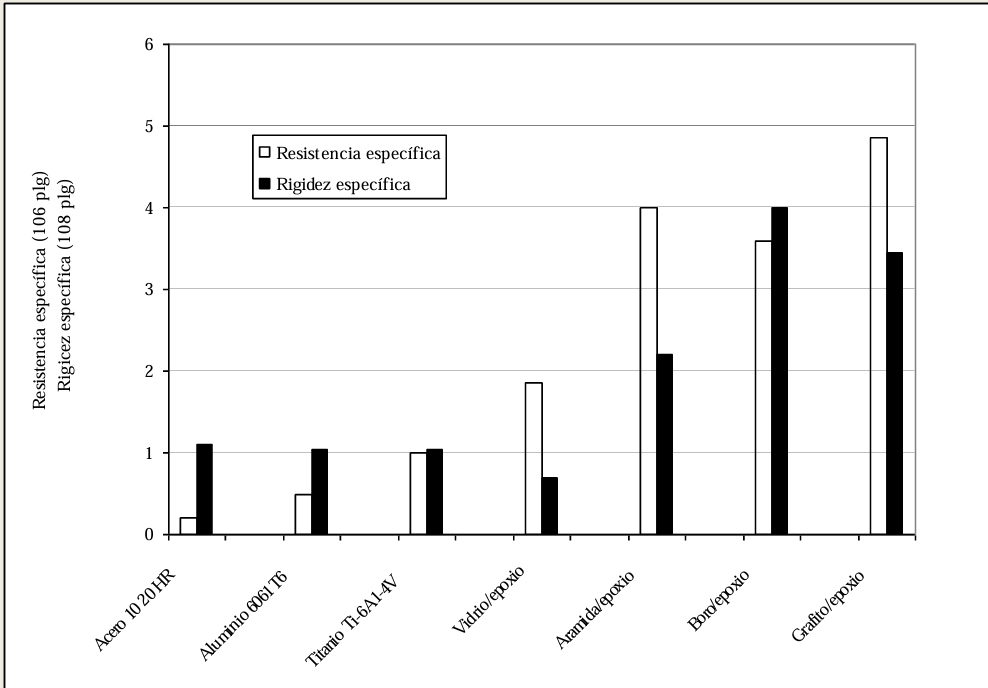
\includegraphics[width=0.4\textwidth]{kevlar.png}
    \caption{Comparativa de resistencia específica y rigidez específica de materiales compuestos y metalicos \\Fuente: diapositivas de la asignatura}
    \label{fig:comparativa_resistencia_rigidez}
\end{figure}

Como puede observarse los primeros muestran mayor resistencia con un menor peso.

\dfn{resistencia especifica}{Resistencia a la traccion dividida por la densidad \\ $\frac{\sigma}{\rho}$}
\dfn{rigidez especifica}{Modulo de Young(elasticidad) dividida por la densidad \\ $\frac{E}{\rho}$}

existen dos tipos de fibra de vidrio, el vidrio E y el vidrio E, La fibra de carbono se obtiene a partir del compuesto orgánico poliacrilonitrilo, mediante el proceso siguiente:
\begin{figure}
    \centering
    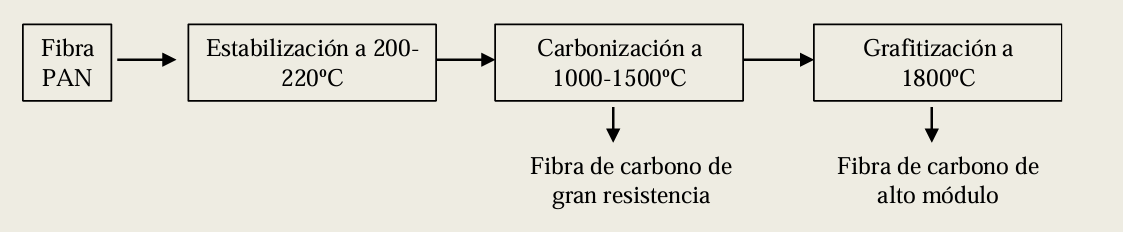
\includegraphics[width=0.4\textwidth]{fibra_de_vidrio.png}
    \caption{Proceso de obtencion de la fibra de vidrio}
    \label{fig:fibra_de_vidrio}
\end{figure}

En primer lugar son estirados y oxidados a temperaturas de 200-220ºC y, tras un proceso de carbonización que elimina O, H y N se produce la grafitización, donde el material sometido a altas temperaturas aumenta el grado de orientación de los cristales tipo grafito dentro de cada fibra.

\nt{Las propiedades mecánicas de los materiales compuestos dependen de su composición siendo asi, intermedias entre las propiedades mecánicas de las fibras y la matriz que forman el material compuesto.}

Por lo general las fibras presentan tensiones de resistencia máxima, límite de proporcionalidad, etc. mucho mayores que las de la matriz que forma el material, presentando el material compuesto un valor intermedio.

\begin{figure}
    \centering
    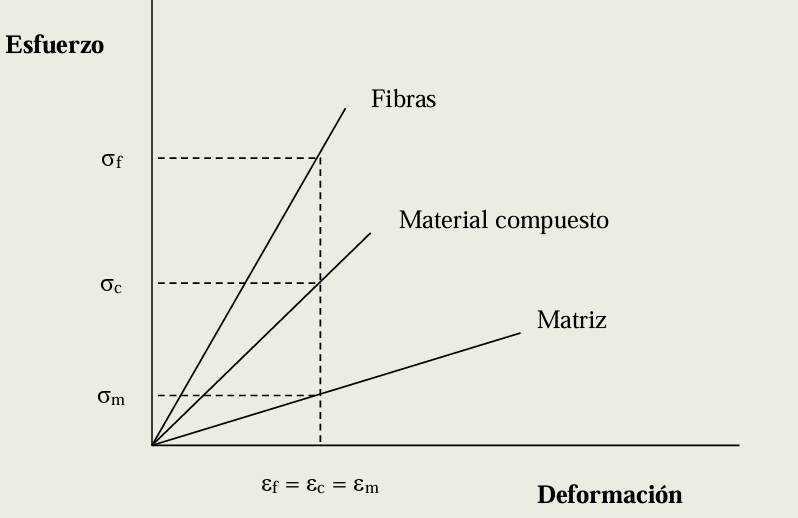
\includegraphics[width=0.4\textwidth]{fibras_vidrio_diagrama_esfuerzo_deformacion.png}
    \caption{Curvas tension-deformacion de materiales compuestos, fibras y matriz \\ Fuente: diapositivas de la asignatura}
    \label{fig:curvas_tension_deformacion}
\end{figure}
Las caracteristicas mas importantes son:
\begin{itemize}
    \item  La \textbf{resistencia máxima a la tracción específica} puede variar hasta cinco veces respecto a las aleaciones de alta resistencia. Los módulos de elasticidad específicos hasta ocho veces.
    \item  Los materiales compuestos pueden funcionar mucho mejor que el acero en aplicaciones donde existen \textbf{cargas cíclicas que produzcan fatiga}.
    \item  Donde se esperen \textbf{cargas de impacto y vibraciones} los materiales compuestos pueden proporcionar un alto nivel de amortiguación.
    \item Como las \textbf{propiedades} de estos materiales \textbf{cambian con la dirección} en las que se colocan las fibras, no son isotropicos, la fabricación de estos materiales se realiza procurando la máxima homogeneidad del material consiguiendo una distribución adecuada de las fibras en el interior del material.
    \item Los \textbf{cambios dimensionales con la temperatura suelen ser menores} en los materiales compuestos que en los metales.
    \item Pueden fabricarse \textbf{estructuras de formas complejas de una sola pieza} lo que reduce el número de operaciones de sujeción, se eliminan las juntas, etc.
\end{itemize}

Aunque estos materiales tienen una serie de \textbf{limitaciones} como son:
\begin{itemize}
    \item \textbf{El coste elevado de las materias primas} de la que están formados.
    \item Su fabricación requiere de \textbf{técnicas más complejas} que las de los materiales convencionales por lo que son distintas y poco generalizadas.
    \item Las \textbf{temperaturas máximas} que pueden soportar los materiales compuestos de matriz polimérica son 260ºC aunque esto puede modificarse con matrices cerámicas o metálicas.
    \item \textbf{Pueden presentar problemas de anisotropía direccional} de sus propiedades \textbf{es decir} que al \textbf{no} ser \textbf{isotrópicas varían con la dirección en la que se aplique la carga}.
    \item El análisis del comportamiento e inspección de estos materiales \textbf{requiere técnicas especiales} que aún no están totalmente desarrolladas.
\end{itemize}
la relacion resistencia coste que hay suele ser mayor en este tipo de materiales.

\subsection{Materiales Semiconductores}
Materiales con \textbf{propiedades de conductividad eléctrica intermedias entre conductores y aislantes fuertemente modulables por dopaje con impurezas atómicas, temperatura o campo eléctrico} (silicio monocristalino, germanio, arseniuro de galio GaAs). Constituyen la base de la instrumentación electrónica, en los \textbf{circuitos integrados} para la industria electrónica y ordenadores. El mas importante de estos es el \textbf{Silicio} puro,
que puede ser modificado para cambiar sus propiedades eléctricas, ya que éstas son extremadamente sensibles a la presencia de átomos de impurezas. También, el germanio, selenio, arseniuro de galio, seleniuro de cinc o teluro de plomo.

\subsection{Tendencia en el uso de materiales y criterios de selección}
los plásticos termoestables pueden utilizarse a temperaturas más altas que los materiales termoplásticos si bien se observa que la temperatura máxima de operación de los distintos materiales termoestables compuestos de matriz polimérica es baja, no superando los 300ºC. Los materiales metálicos son más adecuados cuando se necesitan materiales más resistentes por lo que son los más utilizados en la industria química como componentes fundamentales de las instalaciones.
\section{Aceros, Clasificación y Tratamientos}
\subsection{Sistemas de Clasificación y Nomenclatura (AISI / SAE y UNS)}
Existen organismos internacionales que regulan la nomenclatura de los metales:
\begin{itemize}
    \item \textbf{AISI / SAE:} Clasifica los aceros al carbono y aleados con un código de \textbf{4 dígitos}:
          \begin{itemize}
              \item Los dos primeros dígitos indican los elementos principales de aleación (ej. $10\text{xx}$ para acero al carbono ordinario, $11\text{xx}$ azufre de fácil mecanizado, $41\text{xx}$ cromo-molibdeno, $43\text{xx}$ níquel-cromo-molibdeno).
              \item Los dos últimos dígitos indican el contenido nominal medio de carbono expresado en centésimas de porcentaje (ej. el acero AISI 1020 posee un $0.20\%$ de C; el AISI 1045 un $0.45\%$ de C).
          \end{itemize}
    \item \textbf{Sistema de Numeración Unificada (UNS o SNU):} Código alfanumérico estandarizado por ASTM y SAE compuesto por una letra prefijo y cinco dígitos. Para aceros al carbono se emplea el prefijo \textbf{G} (ej. el AISI 1020 corresponde a UNS G10200). Para aceros inoxidables se emplea el prefijo \textbf{S} (ej. AISI 304 corresponde a UNS S30400).
\end{itemize}
las clasificaciones mas tipicas son la aisi, aa para el aluminio y ASTM
\subsection{Diagrama de Equilibrio Hierro-Carbono (Fe-C)}
Las aleaciones férreas se dividen en función de su porcentaje en masa de carbono:
\begin{itemize}
    \item \textbf{Aceros:} Contenido en carbono inferior al $1.76\%$ (o $2.14\%$ en clasificaciones termodinámicas clásicas).
    \item \textbf{Fundiciones:} Contenido en carbono entre el $2.14\%$ y el $6.67\%$ (límite correspondiente a la formación de cementita pura, $\text{Fe}_3\text{C}$).
\end{itemize}
\nt{lo que quiere es que sepamos que en los aceros de mas de un 6.67\% en carbono no se suele fabricar realmente es mucho mas abajo por que por debajo hay carburo de hierro, en los aceros se considera una aleacion de hierro con carburo de hierro,los que se suelen usar en ingenieria suelen ser de menor de 1.76\% se puede usar de mayor porcentaje que son fundiciones grises por ejemplo para bancos pero al ser demasiado rigidos no son tan utiles en la ingenieria
    para aceros con bajo porcentaje en carbono es ferrita mas carburo de hierro y a mas temperatura ?? si hacemos cambios de temperatura para tratamientos posteriores reducimos las tensiones superficiales pero no cambia la naturaleza}
\subsubsection{Fases y Constituyentes Microestructurales}
\begin{itemize}
    \item \textbf{Ferrita ($\alpha$):} Solución sólida intersticial de carbono en hierro BCC. Es la fase más blanda, dúctil y tenaz del acero (máxima solubilidad de carbono de $0.022\%$ a $727^\circ\text{C}$).
    \item \textbf{Austenita ($\gamma$):} Solución sólida intersticial de carbono en hierro FCC. Estable a alta temperatura (salvo en aceros inoxidables austeníticos estabilizados con Ni a temperatura ambiente). Admite hasta un $2.14\%$ de C disuelto.
    \item \textbf{Cementita ($\text{Fe}_3\text{C}$):} Carburo de hierro intermetálico con $6.67\%$ de C. Es el constituyente más duro ($>60\text{ HRC}$) y quebradizo.
    \item \textbf{Perlita:} Microestructura bifásica laminar formada por láminas alternadas de ferrita y cementita, producto de la descomposición eutectoide de la austenita a $723^\circ\text{C}$ ($0.80\%$ de C).
    \item \textbf{Martensita:} Fase metaestable formada por enfriamiento ultra-rápido (temple) que impide la difusión atómica del carbono, atrapándolo en una estructura tetragonal centrada en el cuerpo (BCT). Presenta extrema dureza pero elevada fragilidad residual.
\end{itemize}

A mayor contenido en carbono (y por consiguiente mayor fracción de cementita y perlita), el acero experimenta un incremento en su resistencia mecánica a la tracción y en su dureza, acompañado por una reducción correlativa de su ductilidad y tenacidad al impacto.

muchas veces no se puede trabajar bien con el material si es demasiado rigido por ello hay que buscar el punto optimo para el trabajo
\subsection{Tipos Principales de Aceros}

\subsubsection{Aceros al Carbono}
\begin{itemize}
    \item \textbf{Bajos en carbono ($\%C < 0.25\%$):} Estructura casi totalmente ferrítica. Muy dúctiles, tenaces, fácilmente conformables en frío y de excelente soldabilidad. Se emplean masivamente en vigas, placas, chapas y tuberías de procesos de baja presión.
    \item \textbf{Medios en carbono ($0.25\% < \%C < 0.60\%$):} Mayor resistencia mecánica y al desgaste. Utilizados en componentes mecánicos sometidos a solicitación dinámica como ejes, árboles de transmisión y engranajes.
    \item \textbf{Altos en carbono ($0.60\% < \%C < 1.40\%$):} Máxima dureza y resistencia, empleados en herramientas de corte, troqueles y resortes.
    \item \textbf{Fundiciones ($\%C > 2.1\%$):} Materiales frágiles con excelente colabilidad y gran amortiguación de vibraciones (utilizadas en bancadas pesadas de maquinaria y carcasas de bombas).
\end{itemize}
/nt{aceros aleados al incluir otras sustancia en general metales para conseguir otros caracter por ejemplo cr para inoxidable wolframio para mayor resistencia mecanica molibdeno y nibio para templabilidad y zonas mas afectadas por la soldadura, vanadio para endurecimiento
acero inoxidable contenido en cromo alto para que sean mas resistentes a la corrosion
}%! Apuntes de clase
\subsubsection{Aceros Inoxidables}
Aleaciones férreas que contienen un mínimo del $10.5\% - 12\%$ de \textbf{cromo}, elemento que reacciona con el oxígeno ambiental formando instantáneamente una capa pasivante nanoscópica de óxido de cromo ($\text{Cr}_2\text{O}_3$) continua, impermeable y autoregenerable que aísla el metal de la corrosión.
\begin{itemize}
    \item \textbf{Martensíticos (Serie AISI 400, ej. 410, 420):} Elevado contenido en carbono. Pueden endurecerse intensamente mediante tratamiento térmico de temple y revenido. Son magnéticos.
    \item \textbf{Ferríticos (Serie AISI 400, ej. 430):} Bajo contenido en carbono y entre $16-18\%$ de Cr. No pueden endurecerse mediante tratamiento térmico. Son magnéticos y se usan en menaje e interiores.
    \item \textbf{Austeníticos (Serie AISI 300, ej. 304, 316):} Los más empleados en la industria química y de procesos. Contienen níquel como estabilizador de la austenita a temperatura ambiente ($18\%\text{ Cr} - 8\%\text{ Ni}$). Son no magnéticos en estado recocido, presentan excelente conformabilidad y tenacidad criogénica extraordinaria.
          \begin{itemize}
              \item \textit{Corrosión por picaduras:} En presencia de cloruros disueltos ($\text{Cl}^-$) el AISI 304 es vulnerable. Para evitarlo se añade entre un $2\%$ y un $3\%$ de \textbf{molibdeno} dando lugar al acero \textbf{AISI 316}.
              \item \textit{Corrosión intergranular y grados bajos en carbono (304L y 316L):} Al calentar o soldar entre $450^\circ\text{C}$ y $850^\circ\text{C}$ precipitan carburos de cromo ($\text{Cr}_{23}\text{C}_6$) en los límites de grano, empobreciendo en cromo las zonas adyacentes y provocando corrosión intergranular. Para evitarlo se recurre a aleaciones de extra-bajo carbono con $\%C \leqslant 0.03\%$ (identificadas con el sufijo \textbf{L}, como el AISI 304L y 316L) o estabilizadas con titanio (AISI 321).
          \end{itemize}
\end{itemize}
%! Apuntes de clase debajo
\nt{Para conseguir ese caracter inoxidable en aceros ya no solo para estructura sino para cierto tipo de maquinaria que va a estar en condiciones muy corrosiva o alimentaria pues serie 400 martensiticos o los ferriticos, los de la serie 300 se suele usar mucho en industria alimentaria serie 304 y 316 los aceros inoxidables son susceptibles a que aparezca corrosion por picadura y se le añade molibdeno}
\subsubsection{Aceros Estructurales ASTM y Perfiles Comerciales}
Estandarizados por la ASTM para edificación y soporte de plantas químicas:
\begin{itemize}
    \item \textbf{ASTM A36:} El acero estructural al carbono más universalmente utilizado ($\sigma_A = 248\text{ MPa}$, $\sigma_M = 400\text{ MPa}$).
    \item \textbf{ASTM A242:} Acero de baja aleación y alta resistencia frente a la corrosión atmosférica a la intemperie (acero tipo \textit{Corten}).
    \item \textbf{ASTM A500 / A501:} Aceros destinados a tubos estructurales conformados en frío y en caliente.
    \item \textbf{ASTM A572:} Acero de alta resistencia de baja aleación al columbio-vanadio (Grados 42, 50, 60 y 65).
\end{itemize}
%! Apuntes de clase debajo
suelen ser parte de equipo angulos barras de sujeccion...  perfiles Hb IBN que son nomenclaturas dependiedo de la forma que tienen.
\textbf{Perfiles estructurales estandarizados más frecuentes:}
\begin{itemize}
    \item \textbf{Perfiles en L (angulares):} Se designan como $\text{L} \, a \times b \times t$ (ej. $\text{L}4 \times 3 \times 1/2$, indicando alas de $4''$ y $3''$ con espesor de $1/2''$).
    \item \textbf{Perfiles en C (canales):} Se designan indicando el peralte y el peso lineal en libras por pie (ej. $\text{C}15 \times 50$, canal de $15''$ de altura y $50\text{ lb/ft}$).
    \item \textbf{Perfiles W (vigas de patín ancho) y S (vigas estándar americanas):} Empleados en vigas principales y columnas resistentes a flexión.
    \item \textbf{Tuberías estructurales cuadradas y rectangulares (HSS):} Gran resistencia bidireccional a torsión y pandeo.
\end{itemize}
%! Apuntes de clase debajo
las vigas de patin ancho se suele usar aunque tenga el mismo material por la forma debido a que la seccion tiene un momento estatico mas elevado, mayor rigidez y soporta mas peso soportan mejor la flexion, tambien comenta un poco lo que son las vigas aligeradas que las tensiones maximas estan en los extremos y por eso se hacen huecos en el centro.
\subsection{Tratamientos de los Aceros}

\subsubsection{Tratamientos Mecánicos}
\begin{itemize}
    \item \textbf{Laminado en caliente (HR - \textit{Hot Rolled}):} Realizado por encima de la temperatura de recristalización. Genera granos equiaxiales libres de tensiones residuales, resultando en un acero blando, dúctil y de menor coste, para reducir espesor o darle mayor resistencia mecanica.
    \item \textbf{Laminado en frío (CR - \textit{Cold Rolled}):} Realizado a temperatura ambiente. Producen acritud intensa, elevando drásticamente el límite elástico y la resistencia a expensas de la ductilidad, con excelentes tolerancias dimensionales,mas severo que en caliente.
    \item \textbf{Estirado en frío (CD - \textit{Cold Drawn}):} Realizado a temperatura ambiente. Producen acritud intensa, elevando drásticamente el límite elástico y la resistencia a expensas de la ductilidad, con excelentes tolerancias dimensionales mas severo que el laminado.
\end{itemize}
%! Apuntes de clase debajo
producir una deformacion plastica para conferir una resistencia mecanica adecuada, al tensar por ejemplo cambia el limite elastico,
el estirado en frio da una resistencia mecanica mayor que los otros, en materiales de misma composicion pero difiriendo el tratamiento mecanico la resistencia sera distinta
\subsubsection{Tratamientos Térmicos}
Modifican la microestructura interna mediante ciclos térmicos controlados de calentamiento, mantenimiento y enfriamiento:
\begin{itemize}
    \item \textbf{Temple y Revenido:} Calentamiento hasta fase austenítica ($800 - 900^\circ\text{C}$) seguido de enfriamiento brusco en agua (WQT) o aceite (OQT) para generar martensita. Dado que la martensita pura es frágil, se aplica inmediatamente un \textbf{revenido} (recalentamiento entre $200^\circ\text{C}$ y $700^\circ\text{C}$) para recuperar tenacidad aliviando tensiones internas.
    \item \textbf{Normalizado:} Calentamiento por encima de la temperatura crítica superior $A_3$ seguido de enfriamiento lento al aire tranquilo. Proporciona grano fino y uniforme, mejorando la maquinabilidad y resistencia al impacto.
    \item \textbf{Recocido completo:} Calentamiento austenítico y enfriamiento extraordinariamente lento dentro del propio horno apagado. Produce la máxima blandura y ductilidad posibles.
    \item \textbf{Recocido de alivio de tensiones:} Calentamiento subcrítico por debajo de $A_1$ ($550 - 650^\circ\text{C}$) para eliminar tensiones residuales derivadas de procesos de soldeo o mecanizado pesado sin alterar la estructura básica del grano.
\end{itemize}
Pretende reducir la dureza debido a que los tratamientos mecanicos generan muchas tensiones residuales, (ejemplo en un vaso si metemos agua hirviendo y hielos continuamente revienta por las tensiones residuales pues esto es lo que se evita con este tratamiento)
calentamiento por debajo de ese limite superior para evitar las tensiones templado, si es mas suave es un normalizado tensiones residuales menores resistencia menor, si se da en el horno se alcnza otras fases por debajo del limite inferior que es un recocido
\subsubsection{Tratamientos Superficiales Termoquímicos}
Incrementan selectivamente la dureza y resistencia al desgaste superficial manteniendo un núcleo interior tenaz y dúctil:
\begin{itemize}
    \item \textbf{Cementación (carburación):} Difusión atómica de carbono en la superficie del acero al calentarlo a $850 - 950^\circ\text{C}$ en atmósfera carburante rica en hidrocarburos ($\text{CH}_4 \rightarrow \text{C} + 2\text{H}_2$), seguido de temple y revenido superficial.
    \item \textbf{Nitruración:} Difusión de nitrógeno atómico a menor temperatura ($500 - 525^\circ\text{C}$) en corriente de amoníaco gas ($2\text{NH}_3 \rightarrow 2\text{N} + 3\text{H}_2$). El nitrógeno precipita formando nitruros duros ($\text{Fe}_4\text{N}$) alcanzando durezas de hasta $80\text{ HRC}$ sin requerir temple posterior.
    \item \textbf{Cianuración:} Formación combinada de carburos y nitruros introduciendo las piezas en un baño de sales fundidas de cianuro a $800 - 900^\circ\text{C}$.
\end{itemize}
pretenden modificar la resistencia de la superficie del metal, por lo general da mayor resistencia a las capas/micras del material, ya que la mayor parte de los fallos del equipo se produce por fatiga qu ees en la superficie del material, se suele tratar la cementacion el acero en alta temperatura se le hace pasar por una corriente de metano para que en la superficie tenga mayor cantidad de carbono (al formarse carburo de hierro en la superficie dando mayor resistencia a la superficie)
con la nitruracion se pretende formar en las micras de la superficie nitruros de hierro a altas temperaturas se pasa amoniaco y reacciona el nitrogeno con el hierro de la superficie aumentando la resistencia mecanicaa y la resis a la corrosion
la cianuracion es cuando se quiere dar ambos Tratamientos

\section{Metodología de Selección de Materiales y Diagramas de Ashby}

La elección final de un material en un proyecto de ingeniería química exige conciliar exigencias multifactoriales: mecánicas (resistencia, rigidez), térmicas, químicas (resistencia a fluidos agresivos), procesabilidad y coste económico.

Para ello se emplea la metodología sistemática propuesta por \textbf{M.~F.~Ashby}, basada en \textbf{diagramas de selección multivariable (Diagramas de Ashby)} que cruzan propiedades contrapuestas en escalas logarítmicas:
\begin{itemize}
    \item Módulo de Young ($E$) frente a densidad ($\rho$) para optimizar componentes con mínima masa y máxima rigidez elástica.
    \item Resistencia mecánica ($\sigma_M$) frente a coste relativo por unidad de volumen.
    \item Empleo de herramientas de software especializado en bases de datos de materiales e índices de mérito (como \textit{Ansys Granta EduPack / CES Selector}).
\end{itemize}
\nt{Para cuando se usa un material para un uso concreto lo mas habitual es ir al fabricante para ese uso concreto aun asi hay usos nuevos donde se necesita elegir el material, hay software y diagramas para seleccionar que tiene en cuenta la densidad y propiedades mecanicas  aunque no entra }


% 3. Problemas resueltos de examen y test de autoevaluación
\clearpage
\section{Problemas Resueltos del Tema 1}

\begin{question}{Módulo de elasticidad a partir de alargamiento en barra recta}{prob:1}
    Una barra recta de sección uniforme está sometida a una fuerza de tracción axial. La sección transversal es de $6\text{ cm}^2$ y la longitud inicial es de $4\text{ m}$. Si el alargamiento total registrado bajo una carga axial de $12\,600\text{ kgf}$ es de $0.40\text{ cm}$, determinar el módulo de elasticidad del material en $\text{kgf}/\text{cm}^2$.
\end{question}

\solve{}
\textbf{1. Datos del problema:}
\begin{itemize}
    \item Sección transversal: $A_0 = 6\text{ cm}^2$
    \item Longitud inicial: $L_0 = 4\text{ m} = 400\text{ cm}$
    \item Carga axial aplicada: $P = 12\,600\text{ kgf}$
    \item Alargamiento elástico total: $\delta = 0.40\text{ cm}$
\end{itemize}

\textbf{2. Ecuaciones fundamentales:}
Asumiendo comportamiento elástico lineal bajo la Ley de Hooke:
\begin{equation*}
    \sigma = E \, \varepsilon \quad \Longleftrightarrow \quad \frac{P}{A_0} = E \, \frac{\delta}{L_0}
\end{equation*}
Despejando el módulo de Young $E$:
\begin{equation*}
    E = \frac{P \cdot L_0}{A_0 \cdot \delta}
\end{equation*}

\textbf{3. Sustitución numérica:}
\begin{equation*}
    E = \frac{12\,600\text{ kgf} \times 400\text{ cm}}{6\text{ cm}^2 \times 0.40\text{ cm}} = \frac{5\,040\,000}{2.4} = 2.10 \times 10^6\text{ kgf}/\text{cm}^2
\end{equation*}
En unidades del Sistema Internacional:
\begin{equation*}
    E \approx 2.10 \times 10^6 \times 9.80665 \times 10^4\text{ Pa} \approx 206\text{ GPa} \quad (\text{correspondiente a un acero})
\end{equation*}


\vspace{1em}

\begin{question}{Compresión uniaxial en cilindro hueco}{prob:2}
    Un cilindro hueco recto de sección circular tiene un diámetro exterior de $7.5\text{ cm}$ y un diámetro interior de $6.0\text{ cm}$. Si se le aplica una fuerza axial de compresión de $5\,000\text{ kgf}$, determinar:
    \begin{enumerate}[label=\alph*)]
        \item La tensión normal de compresión desarrollada.
        \item El acortamiento total que experimenta en una longitud inicial de $50\text{ cm}$.
    \end{enumerate}
    Considérese un módulo de elasticidad $E = 1.05 \times 10^6\text{ kgf}/\text{cm}^2$ y despréciese toda probabilidad de pandeo lateral.
\end{question}

\solve{}
\textbf{1. Datos geométricos y mecánicos:}
\begin{itemize}
    \item Diámetro exterior: $D_{\text{ext}} = 7.5\text{ cm}$
    \item Diámetro interior: $D_{\text{int}} = 6.0\text{ cm}$
    \item Fuerza axial de compresión: $P = 5\,000\text{ kgf}$
    \item Longitud inicial: $L_0 = 50\text{ cm}$
    \item Módulo elástico: $E = 1.05 \times 10^6\text{ kgf}/\text{cm}^2$
\end{itemize}

\textbf{2. Cálculo de la sección transversal neta:}
\begin{equation*}
    A_0 = \frac{\pi}{4} \left(D_{\text{ext}}^2 - D_{\text{int}}^2\right) = \frac{\pi}{4} \left(7.5^2 - 6.0^2\right) = \frac{\pi}{4} (56.25 - 36.00) = \frac{\pi}{4} (20.25) \approx 15.904\text{ cm}^2
\end{equation*}

\textbf{3. Tensión normal de compresión ($\sigma$):}
\begin{equation*}
    \sigma = \frac{P}{A_0} = \frac{5\,000\text{ kgf}}{15.904\text{ cm}^2} \approx 314.38\text{ kgf}/\text{cm}^2 \approx 314.4\text{ kgf}/\text{cm}^2
\end{equation*}

\textbf{4. Acortamiento total elástico ($\delta$):}
Aplicando la relación de Hooke $\sigma = E \, (\delta / L_0)$:
\begin{equation*}
    \delta = \frac{\sigma \cdot L_0}{E} = \frac{314.38\text{ kgf}/\text{cm}^2 \times 50\text{ cm}}{1.05 \times 10^6\text{ kgf}/\text{cm}^2} \approx 0.01497\text{ cm} \approx 0.0150\text{ cm} = 0.15\text{ mm}
\end{equation*}


\vspace{1em}

\begin{question}{Deformación transversal elástica y coeficiente de Poisson en latón}{prob:3}
    Se aplica una carga uniaxial de tracción en la dirección longitudinal de una barra cilíndrica de latón que posee un módulo elástico $E = 10.1 \times 10^4\text{ MPa}$, coeficiente de Poisson $\nu = 0.35$ y un diámetro inicial $d_0 = 10\text{ mm}$. Determinar la magnitud de la carga $P$ necesaria para producir una reducción en el diámetro de $2.5 \times 10^{-3}\text{ mm}$, suponiendo deformación puramente elástica.
\end{question}

\solve{}
\textbf{1. Identificación de magnitudes y datos:}
\begin{itemize}
    \item Módulo de elasticidad: $E = 10.1 \times 10^4\text{ MPa} = 101\,000\text{ N}/\text{mm}^2$
    \item Coeficiente de Poisson: $\nu = 0.35$
    \item Diámetro inicial: $d_0 = 10\text{ mm}$
    \item Variación transversal del diámetro: $\Delta d = -2.5 \times 10^{-3}\text{ mm}$
\end{itemize}

\textbf{2. Deformación unitaria transversal y longitudinal:}
La deformación unitaria lateral en el diámetro es:
\begin{equation*}
    \varepsilon_x = \frac{\Delta d}{d_0} = \frac{-2.5 \times 10^{-3}\text{ mm}}{10\text{ mm}} = -2.5 \times 10^{-4}
\end{equation*}
A partir del coeficiente de Poisson ($\nu = -\varepsilon_x / \varepsilon_z$):
\begin{equation*}
    \varepsilon_z = -\frac{\varepsilon_x}{\nu} = -\frac{-2.5 \times 10^{-4}}{0.35} \approx 7.1429 \times 10^{-4}
\end{equation*}

\textbf{3. Tensión axial requerida ($\sigma_z$):}
Por la ley de Hooke en régimen elástico:
\begin{equation*}
    \sigma_z = E \cdot \varepsilon_z = 101\,000\text{ MPa} \times 7.1429 \times 10^{-4} \approx 72.143\text{ MPa} = 72.143\text{ N}/\text{mm}^2
\end{equation*}

\textbf{4. Cálculo de la carga axial $P$:}
La sección transversal inicial de la probeta es:
\begin{equation*}
    A_0 = \frac{\pi}{4} d_0^2 = \frac{\pi}{4} (10\text{ mm})^2 = 25\pi\text{ mm}^2 \approx 78.54\text{ mm}^2
\end{equation*}
Por tanto, la carga $P$ aplicada resulta:
\begin{equation*}
    P = \sigma_z \cdot A_0 = 72.143\text{ N}/\text{mm}^2 \times 78.54\text{ mm}^2 \approx 5\,666\text{ N} \quad (5.67\text{ kN})
\end{equation*}
\textit{Nota sobre el resultado:} Si el cambio diametral fuese $\Delta d = 2.5 \times 10^{-5}\text{ mm}$, la carga sería $56.66\text{ N}$. Para el valor enunciado en el texto de $2.5 \times 10^{-3}\text{ mm}$, la carga elástica rigurosa es $P = 5\,666\text{ N}$.


\vspace{1em}

\begin{question}{Ductilidad y tensión real de fractura en probeta de acero}{prob:4}
    Una probeta cilíndrica de acero con un diámetro original $d_0 = 12.8\text{ mm}$ se ensaya a tracción uniaxial hasta la fractura, alcanzando una resistencia nominal a la rotura $\sigma_D = 460\text{ MPa}$. Una vez rota la probeta, se mide el diámetro transversal mínimo en la sección de fractura resultando $d_f = 10.7\text{ mm}$. Evaluar:
    \begin{enumerate}[label=\alph*)]
        \item La ductilidad del material expresada mediante el porcentaje de estricción (\%ES).
        \item La tensión real $\sigma_{\text{real}}$ que soportaba la sección de estricción en el instante exacto de la fractura.
    \end{enumerate}
\end{question}

\solve{}
\textbf{1. Datos iniciales y finales:}
\begin{itemize}
    \item Diámetro inicial: $d_0 = 12.8\text{ mm}$
    \item Diámetro final en rotura: $d_f = 10.7\text{ mm}$
    \item Resistencia nominal a rotura: $\sigma_D = 460\text{ MPa} = 460\text{ N}/\text{mm}^2$
\end{itemize}

\textbf{2. Cálculo de áreas transversales inicial y final:}
\begin{align*}
    A_0 & = \frac{\pi}{4} d_0^2 = \frac{\pi}{4} (12.8)^2 \approx 128.68\text{ mm}^2 \\
    A_f & = \frac{\pi}{4} d_f^2 = \frac{\pi}{4} (10.7)^2 \approx 89.92\text{ mm}^2
\end{align*}

\textbf{3. Evaluación del porcentaje de estricción (\%ES):}
\begin{equation*}
    \%ES = \frac{A_0 - A_f}{A_0} \times 100 = \frac{128.68 - 89.92}{128.68} \times 100 = \frac{38.76}{128.68} \times 100 \approx 30.1\% \approx 30\%
\end{equation*}

\textbf{4. Cálculo de la tensión real de fractura ($\sigma_{\text{real}}$):}
La carga total $P_D$ actuante en el momento del colapso se deduce a partir de la tensión nominal de rotura referida al área original:
\begin{equation*}
    P_D = \sigma_D \cdot A_0 = 460\text{ N}/\text{mm}^2 \times 128.68\text{ mm}^2 \approx 59\,192.8\text{ N}
\end{equation*}
La tensión real en la rotura se evalúa dividiendo dicha carga entre la sección transversal final real contraída $A_f$:
\begin{equation*}
    \sigma_{\text{real}} = \frac{P_D}{A_f} = \frac{\sigma_D \cdot A_0}{A_f} = 460 \times \frac{128.68}{89.92} = 460 \times \left(\frac{12.8}{10.7}\right)^2 \approx 460 \times 1.431 \approx 658.2\text{ MPa}
\end{equation*}

\clearpage
\section{Test de Autoevaluación - Tema 1}

\begin{enumerate}[label=\textbf{\arabic*.}]
    \item Los materiales compuestos .....
          \begin{enumerate}[label=\alph*.]
              \item Tienen propiedades homogéneas en todas las direcciones del espacio
              \item \textcolor{red!85!black}{Muestran un buen comportamiento frente a cargas cíclicas.}
              \item Presentan una resistencia específica inferior a la de los metales.
          \end{enumerate}

    \item Si se desea el uso de un material que requiera tener baja densidad y alta flexibilidad, de forma general recurriríamos al uso de un material....
          \begin{enumerate}[label=\alph*.]
              \item Cerámico
              \item \textcolor{red!85!black}{Polimérico termoplástico.}
              \item Polimérico termoestable
          \end{enumerate}

    \item Cuando un material sufre una deformación elástica...
          \begin{enumerate}[label=\alph*.]
              \item \textcolor{red!85!black}{Recupera sus dimensiones al dejar de aplicarse la carga.}
              \item Recupera sus dimensiones siempre que no se haya superado el límite de fluencia o cedencia.
              \item Aumenta su límite de proporcionalidad tras dejar de aplicarse la carga.
          \end{enumerate}

    \item Señale la respuesta correcta:
          \begin{enumerate}[label=\alph*.]
              \item Un mayor valor del módulo de resiliencia indica que el material tiene mayor resistencia a la deformación plástica.
              \item \textcolor{red!85!black}{Un mayor valor del Alargamiento a la rotura y de la Estricción indica que el material es más dúctil.}
              \item Ambas respuestas son correctas
          \end{enumerate}

    \item Señale la respuesta correcta:
          \begin{enumerate}[label=\alph*.]
              \item \textcolor{red!85!black}{El objetivo del ensayo de tracción normalizado permite comparar el comportamiento de materiales entre sí.}
              \item El ensayo tracción-deformación suele mostrar la tensión real que sufre un material en función de su deformación unitaria.
              \item El objetivo del ensayo de tracción normalizado es evaluar el comportamiento que tendrá un material en su uso real.
          \end{enumerate}

    \item Señale la respuesta correcta:
          \begin{enumerate}[label=\alph*.]
              \item \textcolor{red!85!black}{La cianuración es un tratamiento superficial que pretende aumentar la resistencia mecánica de la superficie del acero mediante la inclusión de grupos $\text{CN}^-$ (cianuros) sobre la superficie.}
              \item La nitruración es un tratamiento superficial que pretende aumentar la resistencia mecánica de la superficie del acero mediante la formación de nitratos con base férrea.
              \item La cementación es un tratamiento superficial que pretende aumentar la resistencia mecánica de la superficie del acero mediante la formación de carburo de hierro.
          \end{enumerate}

    \item Señale la respuesta correcta:
          \begin{enumerate}[label=\alph*.]
              \item \textcolor{red!85!black}{Ambas respuestas son correctas}
              \item Un aumento en el contenido en carbono de los aceros los hace menos tenaces.
              \item Un material es más tenaz cuando es capaz de absorber mayor energía plástica y elástica antes de su rotura.
          \end{enumerate}

    \item Los materiales compuestos .....
          \begin{enumerate}[label=\alph*.]
              \item Están formados por un material que le confiere rigidez (fibras) y otro que actúa de relleno.
              \item \textcolor{red!85!black}{Suelen tener una resistencia mecánica intermedia entre las fibras y la matriz}
              \item Ambas respuestas son correctas
          \end{enumerate}

    \item Señale la respuesta correcta:
          \begin{enumerate}[label=\alph*.]
              \item Ambas respuestas son correctas
              \item La tenacidad es la capacidad de un material de absorber energía plástica antes de su fractura.
              \item \textcolor{red!85!black}{La tenacidad se puede evaluar mediante ensayos que miden la energía de impacto de un martillo sobre el material}
          \end{enumerate}

    \item Señale la respuesta correcta:
          \begin{enumerate}[label=\alph*.]
              \item \textcolor{red!85!black}{La deformación plástica aumenta el límite elástico de un material}
              \item La deformación plástica disminuye el límite de proporcionalidad de un material.
              \item La deformación plástica reduce el punto de fluencia de un material
          \end{enumerate}

    \item Señale la respuesta correcta:
          \begin{enumerate}[label=\alph*.]
              \item Un aumento de la carga en el ensayo de termofluencia conlleva una reducción de la mínima rapidez de termofluencia
              \item \textcolor{red!85!black}{La termofluencia conlleva el endurecimiento del material debido a la deformación plástica sufrida.}
              \item La mínima rapidez de termofluencia se produce en las etapas iniciales del ensayo de termofluencia, y nos permitirá evaluar el tiempo de vida que tendría un equipo.
          \end{enumerate}

    \item Señale la respuesta correcta:
          \begin{enumerate}[label=\alph*.]
              \item \textcolor{red!85!black}{El ensayo de Erichsen permite evaluar la capacidad que tiene un material plano de ser transformado en piezas huecas como fondos, carcasas, etc.}
              \item El ensayo de flexibilidad permite evaluar las propiedades mecánicas de resistencia que tiene un material.
              \item Dentro de los ensayos no destructivos podemos encontrar el ensayo de dureza Rockwell superficial
          \end{enumerate}

    \item Señale la respuesta correcta:
          \begin{enumerate}[label=\alph*.]
              \item El límite de proporcionalidad y el límite de elasticidad siempre coinciden.
              \item \textcolor{red!85!black}{El límite de fluencia inferior es un punto característico del material}
              \item Ambas respuestas son correctas
          \end{enumerate}

    \item En cuanto a la resistencia por fatiga que tienen los materiales
          \begin{enumerate}[label=\alph*.]
              \item La resistencia a la fatiga dependerá de la resistencia mecánica propia que tenga el material, pero no del ambiente de trabajo en el que desarrolle su labor.
              \item \textcolor{red!85!black}{Superficies más pulidas conllevarán mayor resistencia a la fatiga.}
              \item Los procesos superficiales de carburación, nitruración, etc. no mejora la resistencia a la fatiga del material ya que la resistencia mecánica del material completo sigue siendo la misma.
          \end{enumerate}

    \item La tensión ingenieril se define como:
          \begin{enumerate}[label=\alph*.]
              \item Ambas son incorrectas
              \item \textcolor{red!85!black}{Cociente entre la carga aplicada y la sección (inicial) del material transversal a la dirección de aplicación de la carga.}
              \item Cociente entre la carga aplicada y la sección (en cada momento del ensayo) del material transversal a la dirección de aplicación de la carga.
          \end{enumerate}

    \item Señale la respuesta correcta:
          \begin{enumerate}[label=\alph*.]
              \item Un aumento de la temperatura hace que generalmente los materiales sean más rígidos.
              \item \textcolor{red!85!black}{Los ensayos de termofluencia permiten evaluar el comportamiento de un material frente a temperaturas y cargas elevadas en función del tiempo.}
              \item Ambas respuestas son correctas
          \end{enumerate}

    \item Señale la respuesta correcta:
          \begin{enumerate}[label=\alph*.]
              \item El laminado del acero tiene como objetivo la reducción del espesor de la plancha de metal
              \item \textcolor{red!85!black}{El carácter inoxidable de un acero se lo da el contenido en cromo en la aleación, que suele estar entre en una proporción de 10-27\%.}
              \item Uno de los aceros inoxidables más utilizados en la industria alimentaria es el AISI 9228.
          \end{enumerate}

    \item Señale la respuesta correcta:
          \begin{enumerate}[label=\alph*.]
              \item La deformación unitaria se define como el cociente entre el alargamiento y la longitud inicial de la probeta
              \item \textcolor{red!85!black}{Ambas son correctas}
              \item El alargamiento o deformación se define como la elongación que sufre un material en la dirección de aplicación de la carga
          \end{enumerate}

    \item Señale la respuesta correcta:
          \begin{enumerate}[label=\alph*.]
              \item La resistencia máxima a la tracción es el punto donde la tensión real aplicada es máxima
              \item Ambas respuestas son correctas
              \item \textcolor{red!85!black}{En caso de que el límite de fluencia no esté claro, se puede definir como la tensión para la cual la deformación plástica es del 0.2\%.}
          \end{enumerate}

    \item Señale la respuesta correcta:
          \begin{enumerate}[label=\alph*.]
              \item Un aumento de la temperatura en el ensayo de termofluencia conlleva una reducción de la mínima rapidez de termofluencia
              \item La fluencia lenta o termofluencia es mayor en las etapas iniciales del ensayo
              \item \textcolor{red!85!black}{La mínima rapidez de termofluencia nos muestra el crecimiento exponencial de la deformación que sufre un material.}
          \end{enumerate}

    \item Si se desea el uso de un material que requiera tener alta dureza, resistencia al desgaste y con propiedades aislantes y térmicas, de forma general recurriríamos al uso de un material....
          \begin{enumerate}[label=\alph*.]
              \item Polimérico
              \item Metálico
              \item \textcolor{red!85!black}{Cerámico}
          \end{enumerate}

    \item Señale la respuesta correcta:
          \begin{enumerate}[label=\alph*.]
              \item La tensión de trabajo coincide con la tensión en el punto de fluencia o con la resistencia máxima a la tracción, seleccionándose uno de estos valores en función de las condiciones de servicio del material.
              \item \textcolor{red!85!black}{La tensión de seguridad o tensión de trabajo es la tensión máxima que puede soportar un material en sus condiciones de servicio.}
              \item El producto de la tensión en el punto de fluencia o en el punto de máxima tracción (dependiendo del material y uso del mismo) por el coeficiente de seguridad nos determinará la tensión de trabajo del material.
          \end{enumerate}

    \item El acero es una aleación hierro-carbono donde.....
          \begin{enumerate}[label=\alph*.]
              \item Cuanto mayor porcentaje en carbono mayor presente, mayor resistencia mecánica tendrá el material
              \item \textcolor{red!85!black}{Ambas respuestas son correctas}
              \item La ferrita es hierro casi puro y la cementita es un carburo de hierro
          \end{enumerate}

    \item Señale la respuesta correcta:
          \begin{enumerate}[label=\alph*.]
              \item Ambas respuestas son correctas
              \item \textcolor{red!85!black}{La ductilidad es una medida de la deformación plástica que sufre un material antes de su fractura.}
              \item La tenacidad es una medida de la deformación elástica que sufre un material antes de su fractura.
          \end{enumerate}

    \item Señale la respuesta correcta:
          \begin{enumerate}[label=\alph*.]
              \item \textcolor{red!85!black}{Los tratamientos mecánicos tienen como objetivo producir una deformación plástica en el material para conferir una resistencia determinada.}
              \item Un enfriamiento rápido del material desde la temperatura crítica máxima tiene como objetivo reducir las tensiones residuales que aparecen en el material tras un proceso térmico más severo.
              \item Los tratamientos superficiales aplicados a aceros pretenden dar al material una mayor resistencia mecánica al material debido a la deformación plástica que sufre la superficie.
          \end{enumerate}

    \item Ensayo de microdureza:
          \begin{enumerate}[label=\alph*.]
              \item \textcolor{red!85!black}{Vickers y Knoop}
          \end{enumerate}
\end{enumerate}



\chapter{Resistencia Química de Materiales. Corrosión}

\section{Introducción y Relevancia en la Ingeniería Química}

La \textbf{corrosión} es un fenómeno natural y espontáneo por medio del cual los sistemas químicos manifiestan su tendencia termodinámica hacia un estado de equilibrio de menor energía libre. En el ámbito de los materiales y la ingeniería de procesos, se define como:

\dfn{Corrosión}{Reacción química o electroquímica entre un material (principalmente metálico) y su entorno o medio de contacto, que provoca el deterioro progresivo de sus propiedades físicas, químicas y mecánicas.}

La mayor parte de los procesos de corrosión se manifiestan en los materiales metálicos, efectuándose este ataque mediante mecanismos \textbf{electroquímicos} (en presencia de un electrolito) o por \textbf{ataque químico directo} (especialmente a temperaturas elevadas o en medios no polares). 

Sin embargo, los materiales no metálicos también experimentan procesos de degradación química directa:
\begin{itemize}
    \item \textbf{Materiales cerámicos y refractarios:} No sufren corrosión electroquímica al no poseer electrones libres de conducción, pero son atacados químicamente por sales fundidas a elevadas temperaturas, medios fuertemente básicos y ácidos específicos como el ácido fluorhídrico ($\text{HF}$).
    \item \textbf{Polímeros y elastómeros:} No sufren corrosión electroquímica; su deterioro se denomina \textbf{degradación}, producida por absorción de agua, disolventes orgánicos (hinchamiento y disolución) o por escisión de cadenas macromoleculares ante la acción combinada de radiación ultravioleta (UV) y oxígeno (por ejemplo, fragilización del PVC expuesto a la intemperie).
\end{itemize}

\nt{En la industria química, los materiales resistentes a la corrosión suelen presentar costes muy elevados o baja resistencia a las cargas mecánicas. Por tanto, el diseño de equipos implica un compromiso técnico-económico: seleccionar un material resistente mecánicamente (como aceros al carbono o de baja aleación) y prever un sobreespesor por corrosión (\textit{corrosion allowance}), o aplicar recubrimientos y métodos de protección adecuados.}

\subsection{Impacto socioeconómico de la corrosión}
El estudio de la corrosión abarca dimensiones económicas, de seguridad técnica y medioambientales:
\begin{itemize}
    \item \textbf{Impacto en el PIB:} Las pérdidas anuales causadas por corrosión en países industrializados y en vías de desarrollo se estiman en torno al \textbf{3.5\% del Producto Interior Bruto (PIB)}.
    \item \textbf{Consumo de recursos:} Entre \textbf{1/4 y 1/3 de la producción mundial de acero} se destina exclusivamente a la reposición de componentes e infraestructuras metálicas deterioradas.
\end{itemize}

\begin{figure}[H]
    \centering
    \begin{tikzpicture}[node distance=2.5cm, auto, >=Latex]
        \node [draw, rectangle, rounded corners, fill=blue!10, text width=5cm, align=center, thick] (mineral) {\textbf{Metales en la Naturaleza}\\(Óxidos, hidróxidos, sales)\\\textit{Compuestos de baja energía / Estables}};
        \node [draw, rectangle, rounded corners, fill=red!10, text width=5cm, align=center, thick, below of=mineral, yshift=-1cm] (puro) {\textbf{Metales Puros / Aleaciones}\\(Estado metaestable)\\\textit{Mayor contenido energético}};
        
        \draw [->, line width=1.5pt, blue!70!black] (mineral) -- node[midway, right, align=left] {\textbf{Metalurgia Extractiva}\\(Aporte de energía / Reducción)} (puro);
        \draw [->, line width=1.5pt, red!70!black] ([xshift=-1.5cm]puro.north) -- node[midway, left, align=right] {\textbf{Corrosión}\\(Proceso espontáneo $\Delta G < 0$)\\(Retorno al estado combinado)} ([xshift=-1.5cm]mineral.south);
    \end{tikzpicture}
    \caption{Ciclo metalúrgico y naturaleza termodinámica de la corrosión.}
    \label{fig:ciclo_corrosion}
\end{figure}

\subsection{Pérdidas económicas por corrosión}
Las pérdidas económicas provocadas por la corrosión se clasifican en:
\begin{enumerate}
    \item \textbf{Pérdidas directas:}
          \begin{itemize}
              \item Reposición y sustitución de maquinaria, tuberías, válvulas y estructuras colapsadas.
              \item Aplicación periódica de pinturas, revestimientos e inhibidores químicos.
              \item Sobrecoste por el empleo de aleaciones especiales de alta gama (aceros inoxidables austeníticos, titanio, inconel, hastelloys).
          \end{itemize}
    \item \textbf{Pérdidas indirectas:}
          \begin{itemize}
              \item \textbf{Paradas de planta no programadas:} Lucro cesante e interrupción del proceso productivo para reparar fugas o sustituir elementos críticos.
              \item \textbf{Pérdidas de producto y fugas:} Fugas en conducciones y tanques presurizados, con riesgo añadido de contaminación y explosiones.
              \item \textbf{Pérdidas de eficiencia y rendimiento térmico:} Acumulación de costras de óxido e incrustaciones en tubos de intercambiadores de calor, reduciendo drásticamente el coeficiente global de transmisión de calor ($U$).
              \item \textbf{Sobredimensionamiento de equipos:} Incremento excesivo de espesores de pared por desconocimiento o incertidumbre en las velocidades reales de corrosión.
          \end{itemize}
\end{enumerate}

%=============================================================================
\section{Ensayos de Corrosión}

Los objetivos fundamentales de los ensayos de corrosión en ingeniería son:
\begin{itemize}
    \item Seleccionar el material idóneo para una aplicación de proceso concreta.
    \item Evaluar el comportamiento de nuevos materiales y recubrimientos en condiciones límite de operación.
    \item Determinar la agresividad de reactivos, productos intermedios y contaminantes en planta.
    \item Investigar y modelizar los mecanismos cinéticos y electroquímicos de degradación.
\end{itemize}

\subsection{Clasificación de los ensayos de corrosión}
Para que los resultados sean reproducibles, comparables y fiables, los ensayos deben estar estrictamente normalizados según organismos internacionales como la \textbf{NACE} (\textit{National Association of Corrosion Engineers}), la \textbf{ASTM} y el \textbf{MTI} (\textit{Materials Technology Institute}).

\begin{enumerate}
    \item \textbf{Ensayos de laboratorio:} Realizados sobre probetas estandarizadas a pequeña escala bajo condiciones controladas (temperatura, concentración, pH, agitación). Su objetivo principal es el \textbf{cribado previo y descarte} de materiales inadecuados.
    \item \textbf{Ensayos en planta piloto:} Son los más representativos y deseables antes de la construcción industrial, ya que reproducen de forma fidedigna los gradientes térmicos reales, velocidades de flujo, impurezas de materias primas y relaciones área/volumen de la instalación definitiva.
    \item \textbf{Ensayos en planta en servicio:} Técnicas de monitorización \textit{in situ} sobre equipos reales en operación mediante cupones de corrosión, sondas de resistencia eléctrica o ensayos no destructivos (ultrasonidos, corrientes inducidas, radiografía).
\end{enumerate}

\subsection{Variables experimentales que influyen en el ensayo}
\begin{itemize}
    \item \textbf{Caracterización de la muestra:} Composición química exacta, tratamiento térmico previo, tamaño de grano y microestructura. Probetas de referencia archivadas y perfectamente trazables.
    \item \textbf{Preparación superficial:} Superficie pulida y desengrasada. El acabado pulido estandarizado minimiza la rugosidad; para trasladar datos a escala real debe emplearse un \textbf{factor de corrección de laboratorio} (que puede variar de 1 a 10).
    \item \textbf{Técnicas de fijación y exposición:} Las probetas deben sumergirse totalmente aisladas de soportes metálicos mediante materiales plásticos o cerámicos (teflón) para evitar la formación espuria de pilas galvánicas.
    \item \textbf{Tiempo de ensayo:} La velocidad de corrosión suele ser elevada en las fases iniciales y decrecer conforme se forman productos de corrosión. Generalmente se realizan ensayos en \textbf{5 períodos de 48 horas}, renovando la disolución corrosiva en cada ciclo. De forma empírica, el tiempo mínimo de ensayo se evalúa mediante:
          \begin{equation}
              t_{\text{mínimo}} \text{ [horas]} = \frac{2000}{\text{velocidad de corrosión esperada [mpy]}}
              \label{eq:tiempo_minimo_ensayo}
          \end{equation}
    \item \textbf{Aireación:} La presencia de oxígeno disuelto incrementa sensiblemente la corrosión en aceros al carbono, mientras que favorece la pasivación protectora en aluminio y aceros inoxidables. Los ensayos con aireación se realizan burbujeando aire u oxígeno, y los ensayos desaireados burbujeando nitrógeno gaseoso inerte.
    \item \textbf{Limpieza post-ensayo:} Eliminación estricta de productos de corrosión sin desgastar el metal base no atacado mediante limpieza mecánica (cepillos suaves/abrasivos ligeros), química (disolventes/decapantes inhibidos) o electrolítica (polarización catódica de la probeta).
    \item \textbf{Temperatura:} Es una de las variables más críticas. Por regla general, un incremento de temperatura acelera exponencialmente la corrosión (cinética tipo Arrhenius), salvo cuando promueve la formación de fases pasivantes estables o cuando disminuye la solubilidad del oxígeno en líquidos acuosos abiertos (el agua fría abierta retiene más $O_2$ disuelto y puede ser más corrosiva que el agua caliente desoxigenada).
\end{itemize}

\begin{table}[H]
    \centering
    \caption{Efecto de la temperatura en la corrosión del acero inoxidable 18-8S en ácido nítrico al 65\%.}
    \begin{tabular}{cc}
        \toprule
        \textbf{Temperatura ($^\circ$F)} & \textbf{Velocidad de corrosión (mpy)} \\
        \midrule
        Hasta 250 & $< 20$ \\
        260 & 100 \\
        280 & 200 \\
        320 & 500 \\
        330 & 1000 \\
        370 & 5000 \\
        \bottomrule
    \end{tabular}
    \label{tab:efecto_temp_hno3}
\end{table}

\subsection{Expresión cuantitativa y unidades de la velocidad de corrosión}
La velocidad de corrosión uniforme se cuantifica a través de la pérdida de masa por unidad de área y tiempo, traduciéndose a una \textbf{pérdida de espesor por penetración}:

\dfn{Milipulgadas por año (mpy)}{Pérdida de espesor lineal expresada en milésimas de pulgada ($1\text{ mil} = 10^{-3}\text{ in} = 0.0254\text{ mm}$) por año de exposición continua:}
\begin{equation}
    \text{mpy} = \frac{534 \cdot W}{D \cdot A \cdot T}
    \label{eq:mpy_formula}
\end{equation}
donde $W$ es la pérdida de masa en $\text{mg}$, $D$ la densidad del material en $\text{g/cm}^3$, $A$ el área expuesta en $\text{in}^2$ y $T$ el tiempo de ensayo en $\text{horas}$.

En unidades del Sistema Internacional (SI) y normas europeas se emplea la tasa de penetración en $\text{mm/año}$:
\begin{equation}
    \text{Velocidad de penetración } \left[\frac{\text{mm}}{\text{año}}\right] = \frac{87.6 \cdot W}{D \cdot A \cdot T}
    \label{eq:mm_year_formula}
\end{equation}
donde $W$ está en $\text{mg}$, $D$ en $\text{g/cm}^3$, $A$ en $\text{cm}^2$ y $T$ en $\text{horas}$.

\textbf{Factores de conversión de unidades de velocidad de corrosión:}
\begin{equation}
    1\text{ mpy} = 0.0254\text{ }\frac{\text{mm}}{\text{año}} = 25.4\text{ }\frac{\mu\text{m}}{\text{año}} = 2.90\text{ }\frac{\text{nm}}{\text{h}} = 0.805\text{ }\frac{\text{pm}}{\text{s}}
    \label{eq:conversion_corrosion}
\end{equation}

\begin{table}[H]
    \centering
    \caption{Calificación relativa de materiales frente a su resistencia a la corrosión uniforme.}
    \begin{tabular}{lccccc}
        \toprule
        \textbf{Resistencia Relativa} & \textbf{mpy} & \textbf{mm/año} & \textbf{$\mu$m/año} & \textbf{nm/h} & \textbf{pm/s} \\
        \midrule
        \textbf{Excepcional} & $< 1$ & $< 0.02$ & $< 25$ & $< 2$ & $< 1$ \\
        \textbf{Excelente} & $1 - 5$ & $0.02 - 0.1$ & $25 - 100$ & $2 - 10$ & $1 - 5$ \\
        \textbf{Bueno} & $5 - 20$ & $0.1 - 0.5$ & $100 - 500$ & $10 - 50$ & $5 - 20$ \\
        \textbf{Razonable} & $20 - 50$ & $0.5 - 1.0$ & $500 - 1000$ & $50 - 150$ & $20 - 50$ \\
        \textbf{Pobre} & $50 - 200$ & $1.0 - 5.0$ & $1000 - 5000$ & $150 - 500$ & $50 - 200$ \\
        \textbf{Inaceptable} & $> 200$ & $> 5.0$ & $> 5000$ & $> 500$ & $> 200$ \\
        \bottomrule
    \end{tabular}
    \label{tab:clasificacion_resistencia}
\end{table}

%=============================================================================
\section{Fundamentos Termodinámicos y Electroquímicos de la Corrosión}

\subsection{Criterio termodinámico de espontaneidad ($\Delta G$)}
La viabilidad termodinámica de un proceso de corrosión viene determinada por la variación de la \textbf{energía libre de Gibbs} ($\Delta G$). Para una reacción química o electroquímica:
\begin{equation}
    \Delta G = \sum G_{\text{productos}} - \sum G_{\text{reactivos}}
\end{equation}
\begin{itemize}
    \item $\Delta G < 0$: Proceso termodinámicamente espontáneo (tendencia natural a corroerse).
    \item $\Delta G > 0$: Proceso no espontáneo en las condiciones dadas (inmunidad termodinámica).
    \item $\Delta G = 0$: Estado de equilibrio termodinámico.
\end{itemize}

\textbf{Ejemplos termodinámicos de corrosión en medio húmedo con oxígeno:}
\begin{align}
    \text{Mg} + \text{H}_2\text{O} + \frac{1}{2}\text{O}_2 &\longrightarrow \text{Mg(OH)}_2 & \Delta G^\circ &= -142\,600\text{ cal} \quad (\text{Espontánea, alta reactividad}) \\
    \text{Cu} + \text{H}_2\text{O} + \frac{1}{2}\text{O}_2 &\longrightarrow \text{Cu(OH)}_2 & \Delta G^\circ &= -28\,600\text{ cal} \quad (\text{Espontánea, reactividad moderada}) \\
    \text{Au} + \frac{3}{2}\text{H}_2\text{O} + \frac{3}{4}\text{O}_2 &\longrightarrow \text{Au(OH)}_3 & \Delta G^\circ &= +15\,700\text{ cal} \quad (\text{No espontánea, metal noble inmune})
\end{align}

\nt{La energía libre de Gibbs $\Delta G$ indica únicamente la tendencia termodinámica de la reacción, pero \textbf{no predice en absoluto la velocidad con la que se producirá el ataque}. Metales con una $\Delta G$ fuertemente negativa (como el aluminio o el titanio) pueden reaccionar con extrema lentitud debido a la formación instantánea de películas pasivantes de óxido de alta adherencia que bloquean la difusión de reactivos.}

\subsection{Cinética y energía de activación ($Q_0$)}
Para que la reacción tenga lugar es necesario superar una barrera energética o \textbf{energía de activación} ($Q_0$). La constante cinética de velocidad de reacción sigue la ley de Arrhenius:
\begin{equation}
    k = A \cdot e^{-\frac{Q_0}{R \cdot T}}
    \label{eq:arrhenius}
\end{equation}
donde $A$ es el factor preexponencial de frecuencia, $R = 8.314\text{ J/(mol}\cdot\text{K)}$ la constante universal de los gases y $T$ la temperatura absoluta en Kelvin.

\subsection{Naturaleza electroquímica: Semirreacciones redox}
Toda reacción de corrosión en medio húmedo es un proceso electroquímico acoplado que involucra simultáneamente:
\begin{enumerate}
    \item \textbf{Reacción anódica (Oxidación):} Los átomos metálicos ceden electrones y pasan al electrolito como cationes solvatados. Tiene lugar en las regiones superficiales denominadas \textbf{ánodos}:
          \begin{equation}
              \text{M} \longrightarrow \text{M}^{n+} + n\,e^-
          \end{equation}
    \item \textbf{Reacción catódica (Reducción):} Una especie química presente en el electrolito consume los electrones cedidos por el metal en las zonas superficiales denominadas \textbf{cátodos}:
          \begin{equation}
              \text{Oxidante} + n\,e^- \longrightarrow \text{Reductor}
          \end{equation}
\end{enumerate}

\imp{Por el principio de conservación de la carga y electroneutralidad, \textbf{la velocidad total de oxidación debe ser idéntica a la velocidad total de reducción} en todo instante:
\begin{equation*}
    I_{\text{anódica}} = I_{\text{catódica}} \implies \sum v_{\text{oxidación}} = \sum v_{\text{reducción}}
\end{equation*}}

\subsection{Ecuación de Nernst}
La relación fundamental entre la energía libre de Gibbs y el potencial reversible de celda ($E$) viene dada por:
\begin{equation}
    \Delta G = -n \cdot F \cdot E, \qquad \Delta G^\circ = -n \cdot F \cdot E^\circ
\end{equation}
donde $n$ es el número de electrones transferidos y $F = 96\,485\text{ C/mol} \approx 96\,500\text{ C/mol}$ es la constante de Faraday.

Para una reacción redox general del tipo $a\text{A} + b\text{B} \longleftrightarrow p\text{P} + q\text{Q}$:
\begin{equation}
    E = E^\circ - \frac{R \cdot T}{n \cdot F} \ln \left( \frac{[\text{P}]^p [\text{Q}]^q}{[\text{A}]^a [\text{B}]^b} \right)
    \label{eq:nernst_general}
\end{equation}
A condiciones estándar de temperatura y presión ($T = 298.15\text{ K} = 25^\circ\text{C}$, $1\text{ atm}$), empleando el logaritmo decimal:
\begin{equation}
    E = E^\circ - \frac{0.0592}{n} \log \left( \frac{[\text{P}]^p [\text{Q}]^q}{[\text{A}]^a [\text{B}]^b} \right)
    \label{eq:nernst_25C}
\end{equation}

Para un electrodo metálico puro sumergido en una disolución de sus propios iones ($\text{Me}^{n+} + n\,e^- \longleftrightarrow \text{Me}$), el potencial de reducción reversible es:
\begin{equation}
    E = E^\circ + \frac{0.0592}{n} \log [\text{Me}^{n+}]
    \label{eq:nernst_metal}
\end{equation}

\subsection{Serie electroquímica de potenciales estándar}
Tomando como referencia arbitraria cero el \textbf{Electrodo Estándar de Hidrógeno (EEH)}:
\begin{equation}
    2\text{H}^+ + 2\,e^- \longleftrightarrow \text{H}_2(g) \qquad (E^\circ = 0.000\text{ V})
\end{equation}

\begin{table}[H]
    \centering
    \caption{Potenciales estándar de reducción ($E^\circ$) a 25$^\circ$C.}
    \begin{tabular}{lcr}
        \toprule
        \textbf{Carácter} & \textbf{Semirreacción catódica} & \textbf{$E^\circ$ (V)} \\
        \midrule
        \multirow{5}{*}{\parbox{3cm}{\centering \textbf{Catódicos / Nobles}\\(Inactividad creciente)}} 
        & $\text{Au}^{3+} + 3\,e^- \longrightarrow \text{Au}$ & $+1.420$ \\
        & $\text{O}_2 + 4\text{H}^+ + 4\,e^- \longrightarrow 2\text{H}_2\text{O}$ & $+1.229$ \\
        & $\text{Fe}^{3+} + e^- \longrightarrow \text{Fe}^{2+}$ & $+0.771$ \\
        & $\text{O}_2 + 2\text{H}_2\text{O} + 4\,e^- \longrightarrow 4\text{OH}^-$ & $+0.401$ \\
        & $\text{Cu}^{2+} + 2\,e^- \longrightarrow \text{Cu}$ & $+0.337$ \\
        \midrule
        \textbf{Referencia} & $2\text{H}^+ + 2\,e^- \longrightarrow \text{H}_2(g)$ & $0.000$ \\
        \midrule
        \multirow{5}{*}{\parbox{3cm}{\centering \textbf{Anódicos / Activos}\\(Actividad creciente)}} 
        & $\text{Pb}^{2+} + 2\,e^- \longrightarrow \text{Pb}$ & $-0.126$ \\
        & $\text{Sn}^{2+} + 2\,e^- \longrightarrow \text{Sn}$ & $-0.136$ \\
        & $\text{Ni}^{2+} + 2\,e^- \longrightarrow \text{Ni}$ & $-0.250$ \\
        & $\text{Fe}^{2+} + 2\,e^- \longrightarrow \text{Fe}$ & $-0.440$ \\
        & $\text{Zn}^{2+} + 2\,e^- \longrightarrow \text{Zn}$ & $-0.763$ \\
        & $\text{Al}^{3+} + 3\,e^- \longrightarrow \text{Al}$ & $-1.662$ \\
        \bottomrule
    \end{tabular}
    \label{tab:potenciales_estandar}
\end{table}

\nt{Los elementos con $E^\circ < 0$ son más activos (anódicos) que el hidrógeno y tienden a oxidarse espontáneamente desprendiendo hidrógeno en disoluciones ácidas libres de oxidantes. Los elementos situados más arriba en la tabla tienden a actuar como cátodos y reducirse, mientras que los situados más abajo se oxidan.}

%=============================================================================
\section{Pilas Galvánicas Responsables de la Corrosión}

La corrosión electroquímica requiere la coexistencia de zonas anódicas y zonas catódicas en contacto eléctrico e inmersas en un electrolito conductor. Los tipos de pilas que originan corrosión en la industria son:

\subsection{Pilas galvánicas de dos metales disímiles}
Formadas por dos metales distintos conectados eléctricamente y sumergidos en un electrolito. El metal con potencial de electrodo más electronegativo actúa como ánodo y se corroe aceleradamente.

\ex{Cálculo de la FEM en una pila Zn-Ni}{
Una cuba electrolítica a 25$^\circ$C consta de un electrodo de zinc sumergido en $\text{ZnSO}_4$ $0.1\text{ M}$ ($E^\circ_{\text{Zn}^{2+}/\text{Zn}} = -0.763\text{ V}$) y un electrodo de níquel en $\text{NiSO}_4$ $0.05\text{ M}$ ($E^\circ_{\text{Ni}^{2+}/\text{Ni}} = -0.250\text{ V}$), separados por membrana porosa. Determinar el potencial de la celda.

\textbf{Solución:}
Al comparar potenciales, el $\text{Zn}$ es más electronegativo, actuando como ánodo:
\begin{align*}
    \text{Ánodo (Oxidación):} & \quad \text{Zn} \longrightarrow \text{Zn}^{2+} + 2\,e^- \quad (E^\circ_{\text{ox}} = +0.763\text{ V}) \\
    \text{Cátodo (Reducción):} & \quad \text{Ni}^{2+} + 2\,e^- \longrightarrow \text{Ni} \quad (E^\circ_{\text{red}} = -0.250\text{ V}) \\
    \text{Reacción global:} & \quad \text{Zn} + \text{Ni}^{2+} \longrightarrow \text{Zn}^{2+} + \text{Ni} \quad (E^\circ_{\text{celda}} = 0.763 - 0.250 = +0.513\text{ V})
\end{align*}
Aplicando la ecuación de Nernst:
\begin{equation*}
    E = E^\circ_{\text{celda}} - \frac{0.0592}{2} \log \left( \frac{[\text{Zn}^{2+}]}{[\text{Ni}^{2+}]} \right) = 0.513 - \frac{0.0592}{2} \log \left( \frac{0.1}{0.05} \right) = 0.513 - 0.0296 \log(2) \approx \mathbf{0.504\text{ V}}
\end{equation*}
Al ser $E > 0$, la reacción transcurre espontáneamente con disolución anódica del zinc.
}

\subsection{Reacciones catódicas habituales en medios acuosos}
\begin{table}[H]
    \centering
    \caption{Principales reacciones catódicas según el pH y la presencia de oxidantes.}
    \begin{tabular}{llc}
        \toprule
        \textbf{Tipo de Reacción} & \textbf{Ecuación Química Catódica} & \textbf{$E^\circ$ (V)} \\
        \midrule
        \textbf{1. Deposición metálica} & $\text{M}^{n+} + n\,e^- \longrightarrow \text{M}$ (ej. $\text{Cu}^{2+} + 2e^- \rightarrow \text{Cu}$) & Variable \\
        \textbf{2. Desprendimiento de $\text{H}_2$ (medio ácido)} & $2\text{H}^+ + 2\,e^- \longrightarrow \text{H}_2(g)$ & $0.000$ \\
        \textbf{3. Reducción de $\text{O}_2$ en medio ácido oxidante} & $\text{O}_2 + 4\text{H}^+ + 4\,e^- \longrightarrow 2\text{H}_2\text{O}$ & $+1.229$ \\
        \textbf{4. Reducción de $\text{O}_2$ en medio neutro o básico} & $\text{O}_2 + 2\text{H}_2\text{O} + 4\,e^- \longrightarrow 4\text{OH}^-$ & $+0.401$ \\
        \bottomrule
    \end{tabular}
    \label{tab:reacciones_catodicas}
\end{table}

\subsection{Pilas microscópicas en un metal monofásico (Inhomogeneidades)}
En una pieza de metal aparentemente homogéneo (como zinc o hierro expuesto a un ácido), las inclusiones, bordes de grano, segreganzas químicas o diferencias de tensión local generan una multitud de \textbf{microánodos y microcátodos} microscópicos adyacentes.

En la corrosión del hierro en agua aireada:
\begin{align}
    \text{Ánodo:} & \quad \text{Fe} \longrightarrow \text{Fe}^{2+} + 2\,e^- \quad (E^\circ = +0.440\text{ V}) \\
    \text{Cátodo:} & \quad \text{O}_2 + 2\text{H}_2\text{O} + 4\,e^- \longrightarrow 4\text{OH}^- \quad (E^\circ = +0.401\text{ V})
\end{align}
Los iones $\text{Fe}^{2+}$ y $\text{OH}^-$ reaccionan formando hidróxido ferroso $\text{Fe(OH)}_2$, el cual precipita como una capa porosa y esponjosa que sigue oxidándose con el oxígeno disuelto para formar el \textbf{hidróxido férrico} marrón-rojizo (\textit{herrumbre}):
\begin{equation}
    2\text{Fe(OH)}_2 \downarrow + 2\text{H}_2\text{O} + \text{O}_2 \longrightarrow 2\text{Fe(OH)}_3 \downarrow
\end{equation}

\subsection{Pilas de concentración iónica}
Se producen cuando dos regiones de un mismo metal están en contacto con disoluciones de diferente concentración de sus cationes metálicos.
\begin{itemize}
    \item Según la ecuación de Nernst, la región en contacto con la \textbf{disolución más diluida} presenta un potencial de electrodo más negativo, comportándose como \textbf{ánodo} y corroyéndose.
    \item La región con \textbf{mayor concentración iónica} actúa como \textbf{cátodo}, depositando metal hasta igualar potenciales.
\end{itemize}

\subsection{Celdas de aireación diferencial}
Ocurren cuando existe un gradiente de concentración de oxígeno disuelto en la superficie húmeda de una estructura metálica.
\begin{itemize}
    \item Para la reducción catódica de oxígeno: $E = E^\circ - \frac{0.0592}{2}\log \left(\frac{[\text{OH}^-]^4}{P_{\text{O}_2}}\right)$.
    \item Las zonas con \textbf{mayor concentración o presión parcial de $\text{O}_2$} presentan un potencial más noble y actúan como \textbf{cátodo}.
    \item Las zonas con \textbf{menor concentración de $\text{O}_2$} (fondos de depósitos, acoplamientos roscados, resquicios, bajo capas de lodo o pinturas agrietadas) se convierten en \textbf{ánodos} y sufren un severo ataque localizado.
\end{itemize}

\subsection{Celdas de temperatura diferencial}
Aparecen en intercambiadores de calor y calderas donde una misma pieza metálica opera con gradientes térmicos. Por regla general, la zona a \textbf{mayor temperatura} presenta un potencial de reducción menos negativo y actúa como \textbf{cátodo}, mientras que la zona a \textbf{menor temperatura} suele actuar como \textbf{ánodo} (aunque la polaridad puede invertirse según la aireación y la concentración del electrolito).

%=============================================================================
\section{Diagramas de Pourbaix ($E - \text{pH}$)}

Los diagramas de Pourbaix representan el potencial termodinámico de electrodo ($E$) en función del $\text{pH}$ del medio acuoso a 25$^\circ$C, delimitando las regiones termodinámicas de estabilidad de las especies químicas.

\subsection{Tipos de líneas en los diagramas de Pourbaix}
\begin{enumerate}
    \item \textbf{Líneas horizontales:} Representan equilibrios redox con transferencia de electrones e independientes del $\text{pH}$ (por ejemplo, $\text{Me}^{n+} + n\,e^- \longleftrightarrow \text{Me}$). Su potencial depende exclusivamente de la concentración del catión metálico según Nernst:
          \begin{equation}
              E = E^\circ + \frac{R\cdot T}{n\cdot F}\ln [\text{Me}^{n+}]
          \end{equation}
          Por convenio internacional, la frontera entre corrosión e inmunidad se establece en $[\text{Me}^{n+}] = 10^{-6}\text{ M}$.
    \item \textbf{Líneas verticales:} Representan reacciones de hidrólisis o disolución/precipitación dependientes del $\text{pH}$ pero sin intercambio electrónico (procesos no redox, como $\text{Fe}^{3+} + 3\text{H}_2\text{O} \longleftrightarrow \text{Fe(OH)}_3 + 3\text{H}^+$). Su posición viene fijada por el producto de solubilidad ($K_{ps}$).
    \item \textbf{Líneas oblicuas:} Representan equilibrios que involucran simultáneamente transferencia de electrones e iones $\text{H}^+$ o $\text{OH}^-$ (por ejemplo, $\text{Fe}_2\text{O}_3 + 6\text{H}^+ + 2e^- \longleftrightarrow 2\text{Fe}^{2+} + 3\text{H}_2\text{O}$).
\end{enumerate}

\subsection{Líneas de descomposición del agua}
El comportamiento del agua como disolvente delimita una franja de estabilidad electroquímica comprendida entre dos líneas de trazos:
\begin{itemize}
    \item \textbf{Línea superior (a) - Desprendimiento de $\text{O}_2$:} $\text{O}_2 + 4\text{H}^+ + 4\,e^- \longleftrightarrow 2\text{H}_2\text{O}$
          \begin{equation}
              E_a = 1.229 - 0.0592 \cdot \text{pH} \quad [\text{a } P_{\text{O}_2} = 1\text{ atm}]
              \label{eq:linea_a_pourbaix}
          \end{equation}
          Por encima de la línea (a), el agua se descompone oxidándose a oxígeno gaseoso.
    \item \textbf{Línea inferior (b) - Desprendimiento de $\text{H}_2$:} $2\text{H}^+ + 2\,e^- \longleftrightarrow \text{H}_2(g)$
          \begin{equation}
              E_b = 0.000 - 0.0592 \cdot \text{pH} \quad [\text{a } P_{\text{H}_2} = 1\text{ atm}]
              \label{eq:linea_b_pourbaix}
          \end{equation}
          Por debajo de la línea (b), el agua se reduce termodinámicamente desprendiendo hidrógeno gaseoso.
\end{itemize}

\subsection{Zonas fundamentales del diagrama}
\begin{enumerate}
    \item \textbf{Zona de Inmunidad:} El metal en estado elemental es la fase termodinámicamente estable ($\Delta G > 0$ para su disolución a concentraciones $\geq 10^{-6}\text{ M}$). Para el hierro, la inmunidad se logra a potenciales $E < -0.62\text{ V}$.
    \item \textbf{Zona de Corrosión:} Las especies estables son iones solubles ($\text{Fe}^{2+}$, $\text{Fe}^{3+}$, o ferratos $\text{Fe}_2\text{O}_3\text{H}^-$ en medios fuertemente alcalinos). El metal se disuelve de forma continua.
    \item \textbf{Zona de Pasivación:} Las especies estables son óxidos o hidróxidos sólidos insolubles ($\text{Fe}_2\text{O}_3$, $\text{Al}_2\text{O}_3$, $\text{Cr}_2\text{O}_3$) que forman una película adherente sobre la superficie metálica, reduciendo la velocidad de corrosión a valores prácticamente despreciables.
\end{enumerate}

\imp{
\textbf{Utilidad y limitaciones de los Diagramas de Pourbaix:}
\begin{itemize}
    \item \textbf{Utilidad:} Permiten determinar la dirección espontánea de las reacciones redox, estimar los productos de equilibrio y predecir modificaciones de potencial o $\text{pH}$ para proteger el metal (protección catódica, pasivación o protección anódica).
    \item \textbf{Limitaciones:} Son diagramas estrictamente \textbf{termodinámicos} para metales puros en soluciones acuosas ideales; \textbf{no proporcionan información sobre la velocidad de corrosión} (cinética) ni contemplan la presencia de iones agresivos despasivantes (como los cloruros).
\end{itemize}
}

%=============================================================================
\section{Cinética de la Corrosión y Polarización}

\subsection{Concepto de polarización}
Cuando un metal experimenta corrosión neta, el sistema abandona el equilibrio electroquímico. 

\dfn{Polarización}{Desplazamiento del potencial de electrodo desde su valor de equilibrio termodinámico reversible ($E_0$) hasta un potencial constante de valor intermedio ($E_{\text{corr}}$), estableciéndose un flujo de corriente neto ($I_{\text{corr}}$) proporcional a la velocidad de disolución metálica.}

\subsection{Leyes de Faraday y velocidad de corrosión}
La masa de metal disuelto $w$ en un tiempo $t$ viene dada por la \textbf{Ley de Faraday}:
\begin{equation}
    w = \frac{I \cdot t \cdot M}{n \cdot F} \implies I_{\text{corr}} = \frac{w \cdot n \cdot F}{t \cdot M}
    \label{eq:faraday}
\end{equation}
donde $I$ es la intensidad en amperios, $M$ la masa atómica ($\text{g/mol}$), $n$ la valencia y $F = 96\,500\text{ C/mol}$.

La \textbf{densidad de corriente de corrosión} ($i_{\text{corr}}$) referida al área expuesta $A$ ($\text{cm}^2$) es:
\begin{equation}
    i_{\text{corr}} = \frac{I_{\text{corr}}}{A} \quad [\text{A/cm}^2]
\end{equation}
La velocidad de disolución expresada en $\text{mol/(s}\cdot\text{cm}^2)$ es:
\begin{equation}
    v_{\text{oxidación}} = \frac{i_{\text{corr}}}{n \cdot F}
\end{equation}

\ex{Cálculo de corriente y densidad de corrosión en un tanque}{
Un tanque cilíndrico de acero suave bajo en carbono de $1\text{ m}$ de altura y $50\text{ cm}$ de diámetro contiene agua aireada hasta un nivel de $60\text{ cm}$. Muestra una pérdida de masa por corrosión de $304\text{ g}$ tras 6 semanas. Calcular la intensidad de corrosión y la densidad de corriente ($M_{\text{Fe}} = 55.85\text{ g/mol}$, $n = 2$).

\textbf{Solución:}
\begin{enumerate}
    \item Tiempo total en segundos:
          \begin{equation*}
              t = 6\text{ sem} \cdot 7\text{ días/sem} \cdot 24\text{ h/día} \cdot 3600\text{ s/h} = 3\,628\,800\text{ s}
          \end{equation*}
    \item Intensidad de corriente de corrosión ($I_{\text{corr}}$):
          \begin{equation*}
              I_{\text{corr}} = \frac{w \cdot n \cdot F}{t \cdot M} = \frac{304\text{ g} \cdot 2 \cdot 96\,500\text{ A}\cdot\text{s/mol}}{3\,628\,800\text{ s} \cdot 55.85\text{ g/mol}} = \mathbf{0.289\text{ A}}
          \end{equation*}
    \item Área mojada expuesta a corrosión (fondo circular + pared cilíndrica hasta $60\text{ cm}$):
          \begin{equation*}
              A = \frac{\pi \cdot D^2}{4} + \pi \cdot D \cdot h = \frac{\pi \cdot (50\text{ cm})^2}{4} + \pi \cdot (50\text{ cm}) \cdot (60\text{ cm}) = 1963.5 + 9424.8 = 11\,388.3\text{ cm}^2
          \end{equation*}
    \item Densidad de corriente de corrosión ($i_{\text{corr}}$):
          \begin{equation*}
              i_{\text{corr}} = \frac{0.289\text{ A}}{11\,388.3\text{ cm}^2} = \mathbf{2.53 \times 10^{-5}\text{ A/cm}^2}
          \end{equation*}
\end{enumerate}
}

\subsection{Tipos de polarización}
El proceso de corrosión consta de tres etapas en serie; la etapa más lenta actúa como etapa limitante y determina el tipo de polarización:
\begin{enumerate}
    \item \textbf{Polarización por activación:} Controlada por la velocidad de las reacciones electroquímicas en la interfase metal-electrolito (transferencia de electrones).
    \item \textbf{Polarización por concentración:} Controlada por la velocidad de transporte difusivo de los iones reactivos en el electrolito hacia la superficie del electrodo. Disminuye con el aumento de temperatura y la agitación/velocidad del fluido.
    \item \textbf{Polarización por resistencia (óhmica):} Debida a la caída de tensión en el electrolito o a la resistencia eléctrica que ofrece una película compacta de productos de corrosión depositados sobre los electrodos.
\end{enumerate}

\nt{La \textbf{despolarización} es la eliminación o reducción de la polarización debida a la acción de un agente despolarizador (por ejemplo, el $\text{O}_2$ disuelto actúa como despolarizador catódico al consumir el hidrógeno atómico acumulado).}

%=============================================================================
\section{Formas y Mecanismos de Corrosión}

La clasificación sistemática de los tipos de corrosión se basa en la apariencia morfológica del daño:

\subsection{1. Corrosión Uniforme o Generalizada}
Ataque químico o electroquímico regular sobre toda la superficie expuesta.
\begin{itemize}
    \item Es la forma más común y la que genera \textbf{mayor cantidad de masa de metal disuelta}, pero es la \textbf{menos peligrosa desde el punto de vista del colapso estructural imprevisto}, al ser fácilmente predecible y medible.
    \item Se compensa mediante sobreespesores de diseño y se controla con pinturas, inhibidores y protección catódica.
\end{itemize}

\subsection{2. Corrosión Galvánica o Bimetálica}
Generada por el contacto eléctrico entre dos metales con diferente potencial electroquímico en un electrolito conductor.
\begin{itemize}
    \item El metal anódico (más activo) se corroe aceleradamente, mientras que el catódico (más noble) queda protegido.
    \item \textbf{Efecto del área relativa ($A_{\text{cátodo}}/A_{\text{ánodo}}$):} Un cátodo grande acoplado a un ánodo pequeño produce una densidad de corriente de corrosión extremadamente alta en el ánodo, acelerando catastróficamente su perforación.
    \item \textbf{Prevención:} Emplear metales contiguos en la serie galvánica, aislar eléctricamente las uniones con juntas no conductoras (teflón), asegurar que el área del ánodo sea siempre mucho mayor que la del cátodo, o utilizar ánodos de sacrificio (galvanizado con zinc).
\end{itemize}

\subsection{3. Corrosión por Picaduras (\textit{Pitting})}
Forma de ataque extremadamente localizado que genera cavidades o agujeros profundos en el espesor del material.
\begin{itemize}
    \item \textbf{Peligro:} Provoca fallos catastróficos con \textbf{pérdidas de masa globales mínimas}, siendo muy difícil de detectar visualmente.
    \item \textbf{Mecanismo autocatalítico:} La disolución rápida dentro de la picadura genera un exceso de cationes $\text{M}^{n+}$, provocando la migración de iones cloruro ($\text{Cl}^-$) para mantener la electroneutralidad. La hidrólisis de los cloruros metálicos genera ácido clorhídrico libre ($\text{HCl}$):
          \begin{equation}
              \text{M}^+\text{Cl}^- + \text{H}_2\text{O} \longrightarrow \text{MOH} + \text{H}^+\text{Cl}^-
          \end{equation}
          La acidificación local y la concentración de $\text{Cl}^-$ aceleran la disolución anódica dentro de la picadura, mientras que la superficie exterior circundante actúa como cátodo protector.
    \item \textbf{Factores promotores y prevención:} Favorecida por haluros ($\text{Cl}^-$, $\text{Br}^-$) y condiciones de estancamiento. Se previene con agitación continua y adición de elementos de aleación pasivantes como \textbf{molibdeno} (acero AISI 316 con 2-3\% Mo frente a AISI 304).
\end{itemize}

\subsection{4. Corrosión por Grietas o Rendijas (\textit{Crevice Corrosion})}
Ataque localizado en el interior de intersticios estrechos, uniones roscadas, solapas remachadas o bajo depósitos no metálicos.
\begin{itemize}
    \item Se origina por el rápido agotamiento del oxígeno en el interior de la grieta estancada, formándose una celda de aireación diferencial que evoluciona hacia un mecanismo autocatalítico análogo al de picaduras.
    \item \textbf{Prevención:} Diseñar uniones soldadas a tope continuas en lugar de uniones roblonadas/remachadas, evitar esquinas muertas y emplear juntas no absorbentes (PTFE/Teflón).
\end{itemize}

\subsection{5. Corrosión Filiforme}
Variante especial de corrosión por grietas que avanza en forma de filamentos vermiformes bajo recubrimientos protectores orgánicos (esmaltes, barnices, lacas) en envases de hojalata y aluminio.
\begin{itemize}
    \item \textbf{Mecanismo:} Cabeza activa del filamento a bajo $\text{pH}$ y desaireada (ánodo) y cola pasiva aireada donde precipita $\text{Fe(OH)}_3$ (cátodo).
    \item \textbf{Factores:} Aparece fundamentalmente en atmósferas con \textbf{humedad relativa entre 65\% y 90\%}. No altera la resistencia mecánica pero destruye el aspecto comercial del producto.
\end{itemize}

\subsection{6. Corrosión Intergranular}
Ataque selectivo a lo largo de los límites de grano de una aleación metálica.
\begin{itemize}
    \item \textbf{Sensibilización de aceros inoxidables austeníticos (18-8):} Al calentar o soldar en el rango de $500 - 800^\circ\text{C}$, el carbono difunde hacia los bordes de grano y reacciona con el cromo precipitando carburos de cromo ($\text{Cr}_{23}\text{C}_6$). Las zonas adyacentes al borde de grano se empobrecen en cromo por debajo del \textbf{12\%}, perdiendo su carácter inoxidable y convirtiéndose en microánodos activos frente al resto del grano catódico.
    \item \textbf{Métodos de prevención:}
          \begin{enumerate}
              \item \textbf{Tratamiento térmico de hipertemple/disolución:} Calentar a $1050-1100^\circ\text{C}$ para redisolver los carburos de cromo y enfriar bruscamente con agua.
              \item \textbf{Empleo de aceros estabilizados:} Adición de elementos con mayor avidez por el carbono que el cromo, como titanio (AISI 321) o niobio (AISI 347).
              \item \textbf{Empleo de aceros de muy bajo carbono (\textit{Low Carbon}):} Limitar el contenido de carbono a $C \leq 0.03\%$ (acero AISI 304L o 316L).
          \end{enumerate}
\end{itemize}

\subsection{7. Corrosión Erosiva y Cavitación}
\begin{itemize}
    \item \textbf{Corrosión erosiva:} Aceleración del ataque electroquímico debido al movimiento relativo a alta velocidad de un fluido corrosivo, gases o sólidos en suspensión (\textit{slurries}), que desgastan y arrancan mecánicamente las capas protectoras pasivantes. Es especialmente severa en codos de tuberías, impulsores y válvulas. El hierro con \textbf{14.5\% de Silicio} presenta una resistencia excepcional a este fenómeno.
    \item \textbf{Corrosión por cavitación:} Destrucción de películas protectoras por el colapso violento de burbujas de vapor generadas por variaciones bruscas de presión hidrodinámica (con ondas de choque de hasta $60\,000\text{ psi}$). Se previene aumentando la presión neta positiva de aspiración (NPSH), incrementando diámetros de tubería, evitando cambios bruscos de dirección y empleando materiales de elevada dureza superficial.
\end{itemize}

\subsection{8. Disolución Selectiva o Desaleado}
Eliminación preferencial de un elemento de una aleación sólida. El caso más habitual es la \textbf{descincificación de latones} ($\text{Cu}-\text{Zn}$ 70/30), donde el zinc se disuelve selectivamente dejando una estructura esponjosa de cobre sin resistencia mecánica. Se previene reduciendo el contenido de zinc a $< 15\%$ o añadiendo inhibidores (arsénico, antimonio o fósforo).

\subsection{9. Corrosión Bajo Tensión o Esfuerzo (SCC)}
Agrietamiento y fractura frágil producidos por la acción combinada y simultánea de un \textbf{ambiente corrosivo específico} y \textbf{tensiones mecánicas de tracción} (estáticas o residuales de soldadura/conformado).
\begin{itemize}
    \item \textbf{Naturaleza de los esfuerzos:} Solo las tensiones de \textbf{tracción} (residuales u operacionales) son perjudiciales; los esfuerzos de \textbf{compresión superficial} anulan el agrietamiento.
    \item \textbf{Prevención:} Tratamientos térmicos de recocido de alivio de tensiones, granallado/martilleo superficial con perdigones para inducir tensiones de compresión, o sustitución por aleaciones con alto contenido en níquel (Inconel).
\end{itemize}

\subsection{10. Daño por Hidrógeno}
Deterioro originado por la absorción y difusión de hidrógeno atómico ($\text{H}$) en la red cristalina metálica:
\begin{itemize}
    \item \textbf{Ampollamiento (\textit{Hydrogen Blistering}):} El hidrógeno atómico difunde hacia huecos e inclusiones internas, recombinándose en $\text{H}_2$ gaseoso molecular; al no poder difundir, genera presiones colosales que abomban y rompen la pared metálica.
    \item \textbf{Fragilización por hidrógeno:} Pérdida drástica de ductilidad por formación de hidruros quebradizos (como en titanio).
    \item \textbf{Descarburación:} A alta temperatura y presión, el hidrógeno reacciona con el carbono de los aceros formando metano ($\text{CH}_4$), generando microfisuras internas y pérdida de resistencia. Se evita aleando con cromo y molibdeno.
\end{itemize}

\subsection{11. Oxidación a Alta Temperatura}
Reacción directa del metal con gases oxidantes ($O_2$, $SO_2$, vapor de agua) a elevadas temperaturas formando cascarillas de óxido.
\begin{itemize}
    \item \textbf{Relación de Pilling-Bedworth (P.B.):} Relación entre el volumen del óxido formado y el volumen de metal consumido:
          \begin{equation}
              \text{P.B.} = \frac{V_{\text{óxido}}}{V_{\text{metal}}} = \frac{M_{\text{óxido}} \cdot D_{\text{metal}}}{n_{\text{metal}} \cdot M_{\text{metal}} \cdot D_{\text{óxido}}}
              \label{eq:pilling_bedworth}
          \end{equation}
          \begin{itemize}
              \item $\text{P.B.} < 1$: Óxido poroso y no protector (metales alcalinos, $\text{Na} = 0.58$, $\text{K} = 0.45$).
              \item $\text{P.B.} > 1$ excesivo: Óxido sometido a grandes tensiones de compresión que se agrieta y desprende ($\text{Fe}_2\text{O}_3 = 2.15$).
              \item $\text{P.B.} \approx 1 - 2$: Óxido compacto, adherente y protector ($\text{Al}_2\text{O}_3 = 1.29 - 1.38$).
          \end{itemize}
    \item \textbf{Cinéticas de crecimiento:}
          \begin{itemize}
              \item \textit{Lineal:} $W = k_L \cdot t$ (películas porosas o volátiles, no protectoras).
              \item \textit{Parabólica:} $W^2 = k_p \cdot t + C$ (controlada por difusión iónica a través de la capa de óxido; $\text{Fe}$, $\text{Cu}$, $\text{Co}$).
              \item \textit{Logarítmica:} $W = k_e \log(C\cdot t + A)$ (películas muy delgadas y altamente impermeables a temperatura moderada; $\text{Al}$).
          \end{itemize}
\end{itemize}

%=============================================================================
\section{Métodos de Control y Protección Frente a la Corrosión}

El control de la corrosión debe fundamentarse en análisis técnicos y viabilidad económica:

\subsection{1. Selección de Materiales}
\begin{itemize}
    \item \textbf{Condiciones reductoras o no oxidantes (ácidos libres de aire):} Aleaciones de níquel y cromo (Monel, Hastelloy B).
    \item \textbf{Condiciones oxidantes (ácido nítrico):} Aceros inoxidables con alto contenido en cromo.
    \item \textbf{Condiciones altamente oxidantes y cloruradas a alta temperatura:} Aleaciones de titanio o tántalo.
\end{itemize}

\subsection{2. Modificación del Medio e Inhibidores}
\begin{itemize}
    \item \textbf{Desaireación:} Eliminación de $\text{O}_2$ disuelto en aguas de calderas mediante desgasificadores térmicos o aditivos químicos (\textbf{secuestradores de oxígeno} como sulfito sódico $\text{Na}_2\text{SO}_3$ e hidracina $\text{N}_2\text{H}_4$).
    \item \textbf{Inhibidores de adsorción:} Compuestos orgánicos (aminas) que se adsorben formando una película hidrófoba molecular.
    \item \textbf{Inhibidores anódicos (Pasivadores):} Cromatos, nitratos, fosfatos y silicatos que precipitan sales insolubles sobre los ánodos.
    \item \textbf{Inhibidores catódicos:} Sales de magnesio o zinc que forman hidróxidos insolubles sobre los cátodos locales.
\end{itemize}

\subsection{3. Diseño Geométrico de Equipos}
Reglas fundamentales para minimizar la corrosión:
\begin{itemize}
    \item Prever sobreespesor por corrosión adecuado al tiempo de vida útil.
    \item Diseñar fondos cónicos e inclinados con drenaje completo para evitar zonas de líquido estancado.
    \item Preferir recipientes soldados con soldaduras continuas y sin poros frente a uniones remachadas.
    \item Ubicar calentadores e intercambiadores en el centro del fluido para evitar la formación de puntos calientes en las paredes.
    \item Colocar las entradas de fluidos concentrados lejos de las paredes para prevenir celdas de concentración diferencial.
    \item Usar deflectores y diafragmas de choque frente a turbulencias y cavitación.
\end{itemize}

\subsection{4. Recubrimientos Protectores}
\begin{itemize}
    \item \textbf{Metálicos:} Recubrimientos de sacrificio (\textbf{galvanizado de zinc} sobre acero) o recubrimientos barrera multicapa (como el \textbf{cromado}: capa interior de cobre para adherencia, intermedia de níquel para resistencia a la corrosión y exterior de cromo para acabado y dureza).
    \item \textbf{Inorgánicos:} Aceros vidriados y esmaltes cerámicos de alta inercia química.
    \item \textbf{Orgánicos:} Pinturas, lacas y resinas epoxi. \textit{Precaución:} roturas locales en la pintura generan una relación de áreas muy desfavorable (ánodo microscópico con alta densidad de corriente), acelerando la perforación.
\end{itemize}

\subsection{5. Protección Catódica}
Consiste en forzar a toda la estructura metálica a operar como \textbf{cátodo}, suministrando electrones para desplazar su potencial a la \textbf{zona de inmunidad}:
\begin{enumerate}
    \item \textbf{Corriente impresa:} Se conecta el polo negativo de una fuente de corriente continua a la estructura a proteger y el polo positivo a un ánodo auxiliar inerte (grafito).
    \item \textbf{Ánodos de sacrificio:} Conexión galvánica directa con metales más activos (magnesio, zinc, aluminio) que se disuelven protegiendo al acero.
\end{enumerate}

\subsection{6. Protección Anódica}
Consiste en desplazar controladamente el potencial de un metal activo-pasivo hacia su \textbf{zona de pasivación} mediante una fuente externa conectada al polo positivo y regulada con un \textbf{potenciostato} y electrodo de referencia.
\begin{itemize}
    \item Solo es aplicable a metales con comportamiento activo-pasivo ($\text{Fe}$, $\text{Ti}$, $\text{Cr}$, aceros inoxidables) en medios fuertemente agresivos (como ácido sulfúrico concentrado en tanques y cambiadores de calor).
    \item Requiere densidades de corriente elevadas para alcanzar la pasivación inicial, pero corrientes mínimas para su mantenimiento, resultando muy económica en operación.
\end{itemize}

%=============================================================================
\section{Cuestionario de Autoevaluación del Tema 2}

\begin{enumerate}
    \item Indicar la respuesta correcta:
          \begin{enumerate}[label=\alph*.]
              \item Ambas son correctas
              \item El cromado es un sistema de protección frente a la corrosión mediante el uso de recubrimientos que consiste en la aplicación de una única capa de cromo sobre la superficie del metal, protegiéndolo frente a la corrosión.
              \item \textcolor{red!85!black}{El uso de pinturas o barnices como medio de protección frente a la corrosión puede provocar una corrosión rápida del material en el caso de que aparezcan roturas debido a que aumenta la densidad de corrosión en esa rotura.}
          \end{enumerate}
          \nt{El cromado industrial convencional utiliza tres capas (cobre para adherencia, níquel para resistencia a corrosión y cromo superficial). Una fisura puntual en una pintura genera una relación anódica/catódica muy desfavorable con una densidad de corriente de corrosión extremadamente alta en la rotura.}

    \item Seleccione la afirmación correcta. Tal y como se observa en el diagrama de Pourbaix:
          \begin{enumerate}[label=\alph*.]
              \item El diagrama de Pourbaix del hierro nos indica que el acero puede ser pasivado para cualquier valor de pH elegido, de ahí que su uso sea tan frecuente en la industria química.
              \item Todos los metales cuentan con una zona de pasivación, lo que permite a todos los metales ser protegidos por protección anódica.
              \item \textcolor{red!85!black}{Todos los metales tienen un potencial de inmunidad por debajo del cual se considera que el material no sufre corrosión.}
          \end{enumerate}

    \item La protección anódica:
          \begin{enumerate}[label=\alph*.]
              \item Es aplicable a todos los metales. Consiste en aplicar un potencial hasta conseguir que el metal se encuentre a un potencial y pH donde la especie estable sea un producto de corrosión que proteja al resto del metal.
              \item \textcolor{red!85!black}{Ninguna de las respuestas es correcta.}
              \item Es aplicable a todos los metales. Consiste en aumentar el potencial por encima del potencial de inmunidad de forma que el material quede protegido frente a la corrosión.
          \end{enumerate}
          \nt{La protección anódica \textbf{no} es aplicable a todos los metales, sino únicamente a aquellos que presentan transición activo-pasivo y forman películas pasivantes insolubles y estables en el medio considerado.}

    \item Seleccione la afirmación correcta:
          \begin{enumerate}[label=\alph*.]
              \item \textcolor{red!85!black}{La corrosión intergranular aparece en los límites de grano de los metales, pudiendo eliminar el carácter inoxidable de los aceros por formación de carburos de cromo.}
              \item La corrosión filiforme causa un descenso importante en la resistencia mecánica de los metales que se ven afectados por ella.
              \item Ambas respuestas son correctas.
          \end{enumerate}
          \nt{La corrosión filiforme es un fenómeno superficial bajo recubrimientos que perjudica la estética comercial pero no compromete la resistencia mecánica global.}

    \item Seleccione la afirmación correcta:
          \begin{enumerate}[label=\alph*.]
              \item Ambas respuestas son correctas.
              \item La polarización por activación puede eliminarse fácilmente aumentando la velocidad de flujo que incide en la superficie del metal.
              \item \textcolor{red!85!black}{La polarización se define como el desplazamiento de los potenciales de electrodo desde sus valores de equilibrio a un potencial constante de valor intermedio, creándose en ese punto un flujo de corriente neto.}
          \end{enumerate}
          \nt{Aumentar la velocidad del flujo reduce la polarización por concentración (difusión), pero no la polarización por activación (transferencia de carga).}

    \item Seleccione la afirmación correcta:
          \begin{enumerate}[label=\alph*.]
              \item La disolución selectiva es la eliminación preferencial de un elemento en una aleación, como por ejemplo la eliminación de cobre en los bronces.
              \item \textcolor{red!85!black}{Ambas respuestas son erróneas.}
              \item La corrosión por esfuerzo se produce por la existencia de tensiones elevadas de compresión o tracción en materiales sometidos a altas presiones.
          \end{enumerate}
          \nt{La disolución selectiva típica es la eliminación de zinc en latones (descincificación). La corrosión bajo tensión es promovida exclusivamente por tensiones de tracción, nunca de compresión.}

    \item En una pila galvánica con electrolitos ácidos o alcalinos sin iones metálicos presentes:
          \begin{enumerate}[label=\alph*.]
              \item Ninguna respuesta es correcta.
              \item \textcolor{red!85!black}{En medio neutro o básico en presencia de $\text{O}_2$, el $\text{O}_2$ reacciona con el agua para formar iones $\text{OH}^-$.}
              \item En un medio ácido, la reacción de oxidación será la de $\text{H}^+$ hasta $\text{H}_2$.
          \end{enumerate}
          \nt{La reacción catódica en medio neutro/básico aireado es $\text{O}_2 + 2\text{H}_2\text{O} + 4e^- \longrightarrow 4\text{OH}^-$. En medio ácido, la reducción del protón genera hidrógeno ($2\text{H}^+ + 2e^- \longrightarrow \text{H}_2$).}

    \item Seleccione la afirmación correcta:
          \begin{enumerate}[label=\alph*.]
              \item \textcolor{red!85!black}{Cuando un metal se encuentra enterrado es más susceptible de sufrir corrosión debido a la formación de celdas de concentración diferencial.}
              \item En celdas de temperatura diferencial, las zonas con menor temperatura son las más susceptibles de sufrir corrosión.
              \item Ninguna respuesta es correcta.
          \end{enumerate}

    \item Seleccione la afirmación correcta:
          \begin{enumerate}[label=\alph*.]
              \item \textcolor{red!85!black}{Ambas respuestas son correctas.}
              \item Ante la cavitación podemos optar como medio de prevención la optimización del diseño para evitar turbulencias, mayor espesor en zonas más vulnerables o el uso de materiales más resistentes endurecidos superficialmente.
              \item El hierro con 14.5\% de Si es uno de los materiales más resistentes a la corrosión erosiva.
          \end{enumerate}

    \item Dentro de los distintos tipos de corrosión existentes:
          \begin{enumerate}[label=\alph*.]
              \item La corrosión por picaduras hace que el metal pierda una pequeña cantidad de metal debido a corrosión, pero reduce su sección de forma relevante, por lo que reduce de forma importante la resistencia mecánica del metal.
              \item La corrosión uniforme genera una cantidad muy elevada de productos de corrosión, pero realmente no hace perder una resistencia mecánica importante en el metal.
              \item \textcolor{red!85!black}{Ambas son correctas.}
          \end{enumerate}

    \item La corrosión por esfuerzo:
          \begin{enumerate}[label=\alph*.]
              \item \textcolor{red!85!black}{Ambas respuestas son correctas.}
              \item Cuando los metales son soldados o bien se enfrían rápidamente, son susceptibles a este tipo de corrosión, ya que pueden aparecer tensiones residuales de tracción.
              \item Comienza por la superficie, por lo que la deformación plástica de los metales reduce la aparición de este tipo de corrosión.
          \end{enumerate}

    \item Seleccione la afirmación correcta:
          \begin{enumerate}[label=\alph*.]
              \item Ninguna respuesta es correcta.
              \item La corrosión se produce debido a una reacción electroquímica entre cualquier material (metálico, cerámico o plástico) y su entorno.
              \item \textcolor{red!85!black}{Los materiales cerámicos pueden ser atacados por sales fundidas a altas temperaturas.}
          \end{enumerate}

    \item Seleccione la afirmación correcta:
          \begin{enumerate}[label=\alph*.]
              \item La ecuación de Nernst nos permite determinar la velocidad con que se produce la reacción de corrosión entre un material y su entorno.
              \item \textcolor{red!85!black}{Ninguna respuesta es correcta.}
              \item El diagrama de Pourbaix nos permitirá seleccionar las condiciones en que un material puede ser utilizado (pH y potencial) en un uso industrial, ya que nos indica la velocidad con que se corroe, y por tanto, nos permitirá determinar la vida útil del metal y a partir de ahí el espesor debido a corrosión.
          \end{enumerate}
          \nt{Tanto Nernst como Pourbaix son herramientas estrictamente termodinámicas (indican tendencias y equilibrios), pero no proporcionan información sobre velocidades de reacción ni cinética.}

    \item La protección catódica:
          \begin{enumerate}[label=\alph*.]
              \item \textcolor{red!85!black}{Puede aplicarse mediante el uso de baterías que aporte corriente continua o bien mediante el uso de ánodos de sacrificio.}
              \item Ambas respuestas son correctas.
              \item Es aplicable a todos los metales. Consiste en aumentar el potencial por encima del potencial de inmunidad de forma que el material quede protegido frente a la corrosión.
          \end{enumerate}

    \item Indicar la respuesta correcta:
          \begin{enumerate}[label=\alph*.]
              \item \textcolor{red!85!black}{Ambas respuestas son correctas.}
              \item A menor temperatura los materiales metálicos suelen sufrir menor velocidad de corrosión, salvo cuando están en presencia de disoluciones acuosas y el oxígeno interviene en el proceso de corrosión.
              \item Los materiales cerámicos suelen presentar una buena resistencia a las temperaturas altas y a la corrosión por erosión.
          \end{enumerate}

    \item Selecciona la afirmación correcta:
          \begin{enumerate}[label=\alph*.]
              \item La galvanización es un tratamiento que protege a los metales mediante el recubrimiento de cinc que se corroe y protege al resto del metal.
              \item La corrosión por picaduras está muy influenciada por la presencia de iones de haluros, apareciendo principalmente en el fondo de tanques.
              \item \textcolor{red!85!black}{Ambas respuestas son correctas.}
          \end{enumerate}

    \item Indicar la respuesta correcta:
          \begin{enumerate}[label=\alph*.]
              \item \textcolor{red!85!black}{La descarburación por hidrógeno consiste en la formación de hidrocarburos en aceros debido a la presencia de hidrógeno, altas temperaturas y altas presiones.}
              \item Cuando el coeficiente de Pilling-Bedworth de un metal es próximo a 1 garantiza totalmente que el óxido protege al material y evita su corrosión.
              \item Ambas respuestas son correctas.
          \end{enumerate}
          \nt{Un índice P.B. próximo a 1 es condición necesaria pero no suficiente; la capa debe poseer además buena adherencia, alto punto de fusión, bajo coeficiente de difusión iónica y compatibilidad térmica.}

    \item Para evitar la aparición de corrosión es recomendable:
          \begin{enumerate}[label=\alph*.]
              \item Los puntos de calefacción de los recipientes deben ubicarse en las proximidades de las paredes de forma que se formen puntos calientes cerca de las paredes que evitan la aparición de corrosión por esfuerzo.
              \item \textcolor{red!85!black}{El uso de uniones soldadas en lugar de remachadas, ya que se reduce la corrosión por grieta.}
              \item Soportar los equipos sobre una base de cemento/hormigón en lugar de soportes metálicos: la elección de soportes realizados con cemento/hormigón hace que se reduzca la aparición de corrosión.
          \end{enumerate}

    \item Seleccione la afirmación correcta:
          \begin{enumerate}[label=\alph*.]
              \item Metales con un potencial estándar de reducción positivo tienen mayor tendencia a corroerse que los de potencial estándar de reducción negativo.
              \item Ambas respuestas son erróneas.
              \item \textcolor{red!85!black}{El estaño (potencial estándar de reducción de $-0.136\text{ V}$) se corroería frente al electrodo de referencia $\text{H}^+/\text{H}_2$.}
          \end{enumerate}

    \item Indique la respuesta correcta:
          \begin{enumerate}[label=\alph*.]
              \item El diagrama de Pourbaix nos indica las especies estables en función del pH y potencial del sistema, señalando cuándo un material es apto en uso real para un pH y potencial determinado.
              \item \textcolor{red!85!black}{El diagrama de Pourbaix nos indica las especies estables en función del pH y potencial del sistema, pero no nos indica cuándo un material es apto en uso real para un pH y potencial determinado ya que no considera la velocidad de corrosión.}
              \item El diagrama de Pourbaix nos indica el potencial y pH para el cual la polarización de un metal se alcanza, lo que nos permite seleccionar un material para un uso concreto.
          \end{enumerate}

    \item Si los potenciales estándar de reducción de $\text{Al}^{3+}/\text{Al}$ y $\text{Fe}^{3+}/\text{Fe}^{2+}$ son, respectivamente, $-1.662\text{ V}$ y $+0.771\text{ V}$, la reacción espontánea que se produciría si la concentración de iones es constante es:
          \begin{enumerate}[label=\alph*.]
              \item $\text{Al} + 3\text{Fe}^{2+} \longrightarrow \text{Al}^{3+} + 3\text{Fe}^{3+}$
              \item $\text{Al}^{3+} + 3\text{Fe}^{2+} \longrightarrow \text{Al} + 3\text{Fe}^{3+}$
              \item \textcolor{red!85!black}{$\text{Al} + 3\text{Fe}^{3+} \longrightarrow \text{Al}^{3+} + 3\text{Fe}^{2+}$}
          \end{enumerate}
          \nt{El aluminio posee un potencial estándar mucho más negativo ($-1.662\text{ V}$), por lo que actúa como ánodo cediendo 3 electrones ($\text{Al} \rightarrow \text{Al}^{3+} + 3e^-$), mientras que el $\text{Fe}^{3+}$ actúa como cátodo reduciéndose a $\text{Fe}^{2+}$ ($\text{Fe}^{3+} + e^- \rightarrow \text{Fe}^{2+}$). La suma neta da $\text{Al} + 3\text{Fe}^{3+} \longrightarrow \text{Al}^{3+} + 3\text{Fe}^{2+}$.}
\end{enumerate}

\setcounter{chapter}{7}
% !TeX root = ../apuntes_bloque1.tex
\chapter{Diseño de Elementos Sometidos a Tensión Cortante}

% 1. Definiciones de esfuerzo cortante, planos inclinados y uniones remachadas/atornilladas centradas
% !TeX root = ../../apuntes_bloque1.tex
\section{Definiciones y Esfuerzos en Secciones Inclinadas}

En un elemento estructural sometido a solicitaciones exteriores se pueden desarrollar distintos tipos de tensiones según la orientación relativa entre la fuerza aplicada y la sección resistente considerada:
\begin{itemize}
    \item \textbf{Esfuerzos normales ($\sigma$):} Se desarrollan en barras sometidas a cargas axiales aplicadas a lo largo de su eje longitudinal y actúan perpendicularmente a la sección transversal de la barra.
    \item \textbf{Esfuerzos cortantes o tangenciales ($\tau$):} Una barra soporta un esfuerzo cortante cuando las cargas transversales tienden a producir un corte o deslizamiento relativo a través de una sección $C$ comprendida entre los puntos de aplicación de las fuerzas.
\end{itemize}

\dfn{Tensión Cortante Media ($\tau$)}{Es la resistencia interna tangencial por unidad de área que desarrolla una sección resistente para equilibrar un esfuerzo de corte $P$ paralelo al plano de dicha sección:}
\begin{equation}
    \tau = \frac{P}{A}
    \label{eq:t8_tau_media}
\end{equation}
donde $P$ es la carga en cortante y $A$ es el área de la sección transversal sometida al corte. Ejemplos característicos en Ingeniería Química son los pasadores, chavetas, uniones remachadas (roblonadas) y uniones atornilladas.

\subsection{Tensiones en secciones inclinadas bajo carga axial}
Incluso cuando una barra está sometida únicamente a dos fuerzas axiales $P$ iguales y de sentido contrario a lo largo de su eje longitudinal, si en lugar de considerar la sección recta transversal $A_0$ se estudia una sección inclinada $A_\theta$ que forma un ángulo $\theta$ respecto al plano normal, aparecen simultáneamente tensiones normales y tensiones cortantes.

Cortando la barra por el plano inclinado $A_\theta$ y planteando el equilibrio del sólido libre de la izquierda, la carga axial $P$ se descompone en una componente normal $F$ perpendicular a la sección y una componente tangencial o cortante $V$ contenida en el plano de la sección:
\begin{equation}
    F = P \cos\theta, \qquad V = P \sin\theta
    \label{eq:t8_decomp_FV}
\end{equation}

\begin{figure}[H]
    \centering
    \begin{tikzpicture}[>=Latex, thick]
        % Barra izquierda con corte inclinado theta
        \draw[fill=blue!6, draw=black] (0,-0.85) -- (3.8,-0.85) -- (4.7,0.85) -- (0,0.85) -- cycle;
        \draw[dashed, gray] (0,0) -- (5.3,0);
        \draw[dashed, black!70] (4.25,-1.1) -- (4.25,1.1);
        % Angulo theta (plano inclinado forma angulo 28 deg con la vertical)
        \draw[thin, red!70!black] (4.25,0) ++(90:0.65) arc (90:62:0.65);
        \node[red!70!black, font=\small] at (4.44,0.82) {$\theta$};
        % Fuerza axial P izquierda
        \draw[->, line width=1.4pt, blue!75!black] (-1.2,0) -- (0,0) node[pos=0.35, above] {$P$};
        % Componentes F (normal al plano inclinado: dir -28 deg) y V (tangencial al plano inclinado: dir -118 deg)
        \coordinate (M) at (4.25,0);
        \draw[->, line width=1.4pt, blue!75!black] (M) -- ++(0:1.65) node[right] {$P$};
        \draw[->, line width=1.4pt, myg!80!black] (M) -- ++(-28:1.45) node[below right] {$F = P\cos\theta$};
        \draw[->, line width=1.4pt, myr!85!black] (M) -- ++(62:0.95) node[above right] {$V = P\sin\theta$};
        \node[above left, font=\footnotesize] at (4.55,0.68) {$A_\theta$};
        \node[below, font=\footnotesize] at (2.0,-0.9) {Sección recta $A_0$};
    \end{tikzpicture}
    \caption{Descomposición de una fuerza axial $P$ sobre una sección inclinada $A_\theta$ en sus componentes normal $F$ y cortante $V$.}
    \label{fig:t8_seccion_inclinada}
\end{figure}

\nt{En la Figura~\ref{fig:t8_seccion_inclinada}, si el ángulo del plano inclinado respecto a la normal es $\theta$, la normal exterior al plano forma un ángulo $\theta$ con el eje de la barra, mientras que el plano de corte forma un ángulo $\theta$ con el plano vertical $A_0$. Por geometría básica, la relación entre áreas es $\cos\theta = \dfrac{A_0}{A_\theta} \implies A_\theta = \dfrac{A_0}{\cos\theta}$.}

Sustituyendo $F$, $V$ y $A_\theta = A_0/\cos\theta$, se obtienen las tensiones normal y tangencial en el plano inclinado:
\begin{align}
    \sigma(\theta) &= \frac{F}{A_\theta} = \frac{P \cos\theta}{A_0 / \cos\theta} = \frac{P}{A_0}\cos^2\theta \label{eq:t8_sigma_theta}\\
    \tau(\theta)   &= \frac{V}{A_\theta} = \frac{P \sin\theta}{A_0 / \cos\theta} = \frac{P}{A_0}\sin\theta\cos\theta = \frac{P}{2A_0}\sin(2\theta) \label{eq:t8_tau_theta}
\end{align}

De las ecuaciones~\eqref{eq:t8_sigma_theta} y~\eqref{eq:t8_tau_theta} se deducen dos casos límite fundamentales:
\begin{itemize}
    \item \textbf{Sección transversal recta ($\theta = 0^\circ$):} La tensión cortante es nula ($\tau = 0$) y la tensión normal alcanza su valor máximo absoluto:
          \begin{equation*}
              \sigma_{\text{máx}} = \frac{P}{A_0}
          \end{equation*}
    \item \textbf{Sección a $45^\circ$ ($\theta = 45^\circ$, donde $\sin\theta = \cos\theta = \frac{\sqrt{2}}{2}$):} La tensión cortante alcanza su valor máximo absoluto, igualándose en magnitud a la tensión normal sobre ese plano:
          \begin{equation*}
              \tau_{\text{máx}} = \sigma(45^\circ) = \frac{P}{2A_0}
          \end{equation*}
\end{itemize}

%=============================================================================
\section{Diseño de Uniones Atornilladas y Remachadas}

Muchas estructuras y recipientes de proceso están formados por chapas o perfiles que deben unirse entre sí. En materiales metálicos los medios de unión más habituales son los \textbf{tornillos}, los \textbf{remaches (roblones)} y las \textbf{soldaduras}.

\begin{itemize}
    \item \textbf{Uniones atornilladas:} Se ejecutan mediante tornillos (espiga roscada y cabeza), tuerca y arandela introducidos en agujeros practicados sobre las piezas a unir. Sus dimensiones geométricas y calidades están normalizadas (en España, tradicionalmente mediante la norma MV-106-1968 y posteriormente el Código Técnico y Eurocódigo 3). Permiten un montaje y desmontaje sencillo para mantenimiento.
    \item \textbf{Uniones remachadas o roblonadas:} Se realizan mediante roblones formados por una espiga cilíndrica lisa y una \textbf{cabeza de asiento}. El roblón se calienta a unos $1000\,^\circ\text{C}$, se introduce en caliente a través de los taladros alineados de las chapas y mediante golpeo o prensado del extremo libre de la espiga se conforma una segunda cabeza (cabeza de cierre), asegurando una unión permanente y muy ajustada al enfriar.
\end{itemize}

\subsection{Tipologías constructivas y parámetros geométricos}
Las uniones atornilladas y remachadas trabajan fundamentalmente a cortadura. En función de la línea de acción de la carga pueden estar \textbf{centradas} respecto al centroide del grupo de conectores o sometidas a \textbf{cargas excéntricas}. Atendiendo a la disposición de las chapas, se distinguen dos grandes familias (Figura~\ref{fig:t8_tipos_uniones}):
\begin{enumerate}
    \item \textbf{Uniones por solape:} Una chapa se monta directamente sobre la otra.
    \item \textbf{Uniones a tope:} Las dos piezas principales se enfrentan en el mismo plano y se enlazan mediante uno o dos \textbf{cubrejuntas} (en diseño industrial se emplea doble cubrejuntas para evitar excentricidades fuera del plano y duplicar los planos de corte).
\end{enumerate}

\begin{figure}[H]
    \centering
    \begin{tikzpicture}[>=Latex, thick, scale=0.95]
        % Solape 1 fila (corte lateral)
        \node[font=\bfseries\small] at (2.2, 2.3) {Unión por solape (1 fila)};
        \draw[fill=gray!18] (0.5, 1.35) rectangle (3.0, 1.65);
        \draw[fill=gray!28] (1.6, 1.05) rectangle (4.1, 1.35);
        \filldraw[fill=black!80] (2.2, 0.90) rectangle (2.4, 1.80);
        \filldraw[black] (2.3, 1.80) ellipse (0.18 and 0.08);
        \filldraw[black] (2.3, 0.90) ellipse (0.18 and 0.08);
        \draw[->, blue!70!black] (0.4, 1.50) -- (-0.2, 1.50) node[left] {$P$};
        \draw[->, blue!70!black] (4.2, 1.20) -- (4.8, 1.20) node[right] {$P$};
        \node[font=\footnotesize] at (0.8, 1.82) {$t_2$};
        \node[font=\footnotesize] at (3.8, 0.85) {$t_1$};

        % A tope 1 fila doble cubrejuntas (corte lateral)
        \node[font=\bfseries\small] at (8.7, 2.3) {Unión a tope con doble cubrejuntas (1 fila)};
        \draw[fill=gray!18] (6.2, 1.20) rectangle (8.65, 1.50);
        \draw[fill=gray!18] (8.75, 1.20) rectangle (11.2, 1.50);
        % Cubrejuntas superior e inferior
        \draw[fill=blue!12] (7.2, 1.50) rectangle (10.2, 1.72);
        \draw[fill=blue!12] (7.2, 0.98) rectangle (10.2, 1.20);
        % Dos roblones (uno a cada lado)
        \foreach \rx in {7.9, 9.5}{
            \filldraw[fill=black!80] (\rx-0.09, 0.85) rectangle (\rx+0.09, 1.85);
            \filldraw[black] (\rx, 1.85) ellipse (0.16 and 0.07);
            \filldraw[black] (\rx, 0.85) ellipse (0.16 and 0.07);
        }
        \draw[->, blue!70!black] (6.1, 1.35) -- (5.5, 1.35) node[left] {$P$};
        \draw[->, blue!70!black] (11.3, 1.35) -- (11.9, 1.35) node[right] {$P$};
    \end{tikzpicture}
    \caption{Esquema en sección de una unión por solape (corte simple) y una unión a tope con doble cubrejuntas (corte doble).}
    \label{fig:t8_tipos_uniones}
\end{figure}

Los parámetros geométricos característicos de una unión remachada o atornillada son:
\begin{itemize}
    \item \textbf{Diámetro del roblón ($d$):} Diámetro nominal de la espiga una vez remachada, coincidente con el diámetro del taladro practicado en la chapa.
    \item \textbf{Paso ($p$):} Distancia entre los centros de dos remaches consecutivos de una misma fila.
    \item \textbf{Paso entre filas ($p_t$):} Distancia transversal entre las líneas de centros de dos filas consecutivas.
    \item \textbf{Paso diagonal en unión al tresbolillo ($p_d$):} Distancia entre centros de remaches alternados de dos filas adyacentes dispuestas al tresbolillo.
    \item \textbf{Módulo repetitivo:} Porción mínima elemental de la unión (conjunto de remaches y ancho de chapa $p$) que se repite periódicamente a lo largo de la costura.
    \item \textbf{Espesores de las chapas ($t_1, t_2$):} En los desarrollos se toma por convenio $t_1 < t_2$, por lo que la chapa de espesor $t_1$ es la limitante en aplastamiento y tracción.
    \item \textbf{Número de módulos repetitivos ($n$):} Coincide en general con el número de roblones por fila.
\end{itemize}

\subsection{Hipótesis de diseño y tensiones admisibles}
Para el cálculo analítico de uniones remachadas o atornilladas se asumen las siguientes hipótesis simplificativas:
\begin{enumerate}
    \item El rozamiento existente entre las superficies de las chapas es despreciable.
    \item Los remaches llenan completamente los agujeros practicados.
    \item El reparto de esfuerzos entre conectores es uniforme: cada área resistente toma una fracción proporcional de la carga total.
    \item La resistencia al corte se evalúa mediante la tensión cortante media uniforme en la sección transversal del roblón.
\end{enumerate}

De los materiales que conforman los conectores y las placas se requieren tres tensiones admisibles:
\begin{itemize}
    \item Tensión cortante admisible del roblón o tornillo: $\tau_{\text{adm}}$.
    \item Tensión admisible a tracción de las chapas: $\sigma_{\text{trac,adm}}$.
    \item Tensión admisible a compresión o aplastamiento de las chapas: $\sigma_{\text{comp,adm}}$.
\end{itemize}

Toda unión trabajando bajo una carga total $P$ repartida entre $n$ módulos repetitivos ($P_M = P/n$) puede fallar por cuatro mecanismos diferenciados:
\begin{enumerate}[label=\alph*)]
    \item \textbf{Fallo por cortadura} de los vástagos de los remaches.
    \item \textbf{Fallo por compresión o aplastamiento} de la chapa más delgada tras el remache.
    \item \textbf{Fallo por tracción} de la sección neta de chapa comprendida entre agujeros consecutivos.
    \item \textbf{Fallo por desgarramiento marginal} de la chapa en la zona posterior entre el agujero y el borde libre de la placa.
\end{enumerate}

%-----------------------------------------------------------------------------
\subsection{Unión solapada con una fila de remaches}

Sea una unión por solape con 1 fila de remaches y $n$ módulos repetitivos sometida a una carga centrada total $P$. Cada módulo soporta $P_M = P/n$.

\paragraph{a) Fallo del roblón por cortadura ($R_1$).}
Cada módulo presenta 1 remache con 1 sola sección transversal de corte ($\frac{\pi}{4}d^2$). La tensión cortante actuante y la resistencia máxima por módulo en cortadura son:
\begin{equation}
    \tau = \frac{R_1}{\frac{\pi}{4}d^2} \quad \Longrightarrow \quad R_1 = \tau_{\text{adm}} \cdot 1\text{ fila} \cdot \frac{\pi}{4}d^2
    \label{eq:t8_R1_solape1}
\end{equation}
La capacidad total del sistema de $n$ módulos frente a cortadura es $n \cdot R_1$, y el número mínimo de módulos (o remaches) necesarios para resistir $P$ resulta:
\begin{equation}
    n_{\text{mín}} = \frac{P}{\tau_{\text{adm}} \cdot \frac{\pi}{4}d^2}
\end{equation}

\paragraph{b) Fallo de la chapa por compresión o aplastamiento ($R_2$).}
La fuerza se transmite del vástago a la chapa de menor espesor ($t_1$) proyectada sobre un rectángulo equivalente de área $t_1 \cdot d$:
\begin{equation}
    \sigma_{\text{comp}} = \frac{R_2}{t_1 \cdot d} \quad \Longrightarrow \quad R_2 = \sigma_{\text{comp,adm}} \cdot 1\text{ fila} \cdot t_1 \cdot d
    \label{eq:t8_R2_solape1}
\end{equation}
El sistema completo resiste $n \cdot R_2$, siendo el número mínimo de módulos frente a aplastamiento:
\begin{equation}
    n_{\text{mín}} = \frac{P}{\sigma_{\text{comp,adm}} \cdot t_1 \cdot d}
\end{equation}

\paragraph{c) Rotura por tracción entre remaches ($R_3$).}
En un ancho de módulo igual al paso $p$, la sección transversal neta de la chapa delgada descontando el taladro es $(p - d) \cdot t_1$:
\begin{equation}
    \sigma_{\text{trac}} = \frac{R_3}{(p - d)\cdot t_1} \quad \Longrightarrow \quad R_3 = \sigma_{\text{trac,adm}} \cdot (p - d) \cdot t_1
    \label{eq:t8_R3_general}
\end{equation}
Por tanto, la resistencia global a tracción de la chapa perforada es $n \cdot R_3$, y el número mínimo de módulos para resistir $P$ vale:
\begin{equation}
    n_{\text{mín}} = \frac{P}{\sigma_{\text{trac,adm}} \cdot (p - d) \cdot t_1}
\end{equation}

\paragraph{d) Rotura por desgarramiento del borde de la chapa.}
Para evitar que el remache arranque o desgarre la lengüeta final de chapa situada detrás del agujero, las normas de diseño establecen como distancia mínima al borde libre:
\begin{equation}
    D \ge 2\,d
    \label{eq:t8_distancia_borde}
\end{equation}

\begin{ImportanteBox}[title={Procedimiento General de Diseño Óptimo y Rendimiento de la Unión ($\mu$)}]
    Conocidos el diámetro del roblón $d$, los espesores $t_1, t_2$ y las tensiones admisibles ($\tau_{\text{adm}}, \sigma_{\text{trac,adm}}, \sigma_{\text{comp,adm}}$):
    \begin{enumerate}
        \item Evaluar la resistencia de cada módulo repetitivo a cortadura ($R_1$) y a aplastamiento ($R_2$).
        \item Igualar la menor de las dos anteriores a la resistencia de la chapa a tracción ($R_3$):
              \begin{equation*}
                  \text{mín}(R_1, R_2) = R_3 = \sigma_{\text{trac,adm}} \cdot (p - d) \cdot t_1
              \end{equation*}
              De esta igualdad se despeja el \textbf{paso óptimo $p$} entre roblones de una misma fila, equilibrando los mecanismos de fallo.
        \item Calcular el \textbf{rendimiento o eficacia de la unión ($\mu$)}, definido como la relación porcentual entre la resistencia de la chapa taladrada y la de la chapa continua sin agujeros:
              \begin{equation}
                  \mu = \frac{\sigma_{\text{trac,adm}} \cdot (p - d)\cdot t_1}{\sigma_{\text{trac,adm}} \cdot p \cdot t_1}\cdot 100 = \frac{p - d}{p}\cdot 100
                  \label{eq:t8_rendimiento_union}
              \end{equation}
    \end{enumerate}
\end{ImportanteBox}

%-----------------------------------------------------------------------------
\subsection{Unión solapada con dos filas de remaches enfrentados}
Cada módulo repetitivo engloba \textbf{dos roblones} dispuestos en dos filas paralelas, de modo que para $n$ módulos habrá un total de $2n$ remaches:
\begin{itemize}
    \item \textbf{Cortadura:} La carga $R_1$ del módulo se reparte entre los 2 roblones en corte simple:
          \begin{equation*}
              R_1 = (2\text{ filas}) \cdot \tau_{\text{adm}} \cdot \frac{\pi}{4}d^2
          \end{equation*}
    \item \textbf{Aplastamiento:} Cada módulo cuenta con 2 áreas proyectadas de aplastamiento en la chapa delgada $t_1$:
          \begin{equation*}
              R_2 = (2\text{ filas}) \cdot \sigma_{\text{comp,adm}} \cdot t_1 \cdot d
          \end{equation*}
    \item \textbf{Tracción en la chapa:} La sección neta crítica por módulo sigue siendo $(p - d)t_1$ a lo largo de la fila exterior, por lo que:
          \begin{equation*}
              R_3 = \sigma_{\text{trac,adm}} \cdot (p - d) \cdot t_1
          \end{equation*}
\end{itemize}
\nt{Si la unión tuviera $k$ filas de remaches enfrentados, basta multiplicar las resistencias $R_1$ y $R_2$ del módulo por $k$ filas, manteniéndose invariable la expresión de $R_3$ para la fila más solicitada.}

%-----------------------------------------------------------------------------
\subsection{Unión a tope con una fila de remaches}
Al enfrentar las dos chapas principales con \textbf{doble cubrejuntas} (uno arriba y otro abajo, dimensionados para no ser limitantes frente a la chapa principal de espesor $t_1$), cada lado de la junta transmite la totalidad de la carga $P$, y \textbf{cada roblón ofrece dos secciones transversales de corte} (cortadura doble):
\begin{itemize}
    \item \textbf{Cortadura doble:} Cada remache aporta $2$ planos resistentes:
          \begin{equation*}
              R_1 = (1\text{ fila}) \cdot 2 \cdot \tau_{\text{adm}} \cdot \frac{\pi}{4}d^2
          \end{equation*}
    \item \textbf{Aplastamiento en chapa principal:} La carga se apoya en una sola chapa principal de espesor $t_1$:
          \begin{equation*}
              R_2 = (1\text{ fila}) \cdot \sigma_{\text{comp,adm}} \cdot t_1 \cdot d
          \end{equation*}
    \item \textbf{Tracción en chapa principal:} $R_3 = \sigma_{\text{trac,adm}} \cdot (p - d) \cdot t_1$.
\end{itemize}

%-----------------------------------------------------------------------------
\subsection{Unión a tope con dos filas de remaches}
Cada módulo repetitivo posee 2 roblones por lado de chapa principal, trabajando cada uno de ellos en cortadura doble gracias al doble cubrejuntas:
\begin{itemize}
    \item \textbf{Cortadura doble con 2 filas:} $R_1 = (2\text{ filas}) \cdot 2 \cdot \tau_{\text{adm}} \cdot \frac{\pi}{4}d^2 = 4\,\tau_{\text{adm}}\frac{\pi}{4}d^2$.
    \item \textbf{Aplastamiento:} $R_2 = (2\text{ filas}) \cdot \sigma_{\text{comp,adm}} \cdot t_1 \cdot d$.
    \item \textbf{Tracción:} $R_3 = \sigma_{\text{trac,adm}} \cdot (p - d) \cdot t_1$.
\end{itemize}

\begin{table}[H]
    \centering
    \caption{Resumen comparativo de resistencias por módulo repetitivo en uniones remachadas o atornilladas centradas (para $n$ módulos, $P_{\text{total}} = n\cdot \text{mín}(R_1,R_2,R_3)$).}
    \adjustbox{max width=\textwidth}{%
        \renewcommand{\arraystretch}{1.28}
        \setlength{\tabcolsep}{7pt}
        \small
        \begin{tabular}{@{}lcccc@{}}
            \toprule
            \textbf{Tipo de Unión} & \textbf{\shortstack{Cortadura\\($R_1$)}} & \textbf{\shortstack{Aplastamiento\\($R_2$)}} & \textbf{\shortstack{Tracción neta\\($R_3$)}} & \textbf{\shortstack{Roblones totales\\en la junta}} \\
            \midrule
            Solape (1 fila) & $\tau_{\text{adm}}\,\frac{\pi}{4}d^2$ & $\sigma_{\text{comp,adm}}\,t_1 d$ & $\sigma_{\text{trac,adm}}(p-d)t_1$ & $n$ \\
            Solape (2 filas enfrentadas) & $2\,\tau_{\text{adm}}\,\frac{\pi}{4}d^2$ & $2\,\sigma_{\text{comp,adm}}\,t_1 d$ & $\sigma_{\text{trac,adm}}(p-d)t_1$ & $2n$ \\
            A tope doble cubrejuntas (1 fila) & $2\,\tau_{\text{adm}}\,\frac{\pi}{4}d^2$ & $\sigma_{\text{comp,adm}}\,t_1 d$ & $\sigma_{\text{trac,adm}}(p-d)t_1$ & $2n$ ($n$ por lado) \\
            A tope doble cubrejuntas (2 filas) & $4\,\tau_{\text{adm}}\,\frac{\pi}{4}d^2$ & $2\,\sigma_{\text{comp,adm}}\,t_1 d$ & $\sigma_{\text{trac,adm}}(p-d)t_1$ & $4n$ ($2n$ por lado) \\
            \bottomrule
        \end{tabular}%
    }
    \label{tab:t8_resumen_uniones}
\end{table}

\begin{table}[H]
    \centering
    \caption{Esfuerzos permisibles de diseño para conectores de acero estructural (remaches ASTM A502 y tornillos ASTM A325 / A490).}
    \adjustbox{max width=0.88\textwidth}{%
        \renewcommand{\arraystretch}{1.24}
        \setlength{\tabcolsep}{9pt}
        \small
        \begin{tabular}{@{}llcc@{}}
            \toprule
            \textbf{Tipo de Conector} & \textbf{Designación / Grado} & \textbf{\shortstack{Esfuerzo cortante\\permisible $\tau_{\text{adm}}$ (MPa)}} & \textbf{\shortstack{Esfuerzo de tracción\\permisible $\sigma_{\text{trac,adm}}$ (MPa)}} \\
            \midrule
            \multirow{2}{*}{\textbf{Remaches}} & ASTM A502 Grado 1 & 121 & 159 \\
                                               & ASTM A502 Grado 2 & 152 & 200 \\
            \midrule
            \multirow{2}{*}{\textbf{Tornillos}} & ASTM A325 & 121 & 303 \\
                                                & ASTM A490 & 152 & 372 \\
            \bottomrule
        \end{tabular}%
    }
    \label{tab:t8_esfuerzos_astm}
\end{table}


% 2. Diseño de uniones soldadas, uniones con carga excéntrica y problemas resueltos
% !TeX root = ../../apuntes_bloque1.tex
\section{Diseño de Uniones Soldadas}

La soldadura constituye el procedimiento de unión permanente más empleado en la fabricación de recipientes a presión, conducciones industriales y estructuras metálicas. Durante su ejecución se debe controlar cuidadosamente el proceso térmico para evitar defectos críticos como las \textbf{coqueras} (porosidades producidas por gases ocluidos que originan concentraciones de tensiones, fracturas y focos de corrosión) y las \textbf{tensiones residuales} generadas durante el enfriamiento localizado del metal.

\subsection{Métodos de soldeo}
Según la naturaleza física de la unión y el aporte térmico aplicado, los procedimientos de soldeo se clasifican en cuatro grandes grupos:
\begin{enumerate}[label=\alph*)]
    \item \textbf{Falso soldeo (soldadura heterogénea o \textit{brazing/soldering}):} El metal base no alcanza su temperatura de fusión; la unión se consigue aportando un metal o aleación fundida de menor punto de fusión que moja por capilaridad las superficies preparadas:
          \begin{itemize}
              \item \textit{Soldaduras blandas:} Basadas en aleaciones de plomo y estaño ($\text{Pb--Sn}$). Presentan baja resistencia mecánica y se destinan a estanqueidad o conexiones eléctricas.
              \item \textit{Soldadura fuerte:} Realizada a base de latón (aleación $\text{Cu--Zn}$), ofreciendo una resistencia mecánica notablemente superior.
              \item \textit{Soldadura dura:} Ejecutada a menores temperaturas relativas mediante aleaciones de cobre con proporciones variables de plata ($\text{Cu--Ag}$).
          \end{itemize}
    \item \textbf{Soldadura a presión a alta temperatura (forja / resistencia):} No existe metal de aportación externo; se lleva el metal base a estado plástico o fusión localizada en la interfaz de contacto y se aplica una elevada presión mecánica para consolidar la unión.
    \item \textbf{Soldadura a presión en frío:} Aplicable a metales muy dúctiles y blandos (como aluminio y cobre). Se ejecuta aplicando gran presión superficial sin metal de aportación y en ocasiones bajo temperaturas criogénicas próximas a $-150\,^\circ\text{C}$.
    \item \textbf{Soldadura por fusión:} Es la técnica industrial predominante. Consiste en fundir simultáneamente los bordes del metal base y un metal de aportación compatible, originando al solidificar un baño de fusión continuo con excelentes propiedades de resistencia y tenacidad. El calor se suministra mediante \textbf{arco eléctrico} entre electrodo y piezas, o mediante combustión de mezclas gaseosas de acetileno, hidrógeno o gas de alumbrado con oxígeno (\textbf{soldadura autógena o oxiacetilénica}).
\end{enumerate}

\subsection{Tipos de soldaduras y eficacia de junta ($E_S$)}
En el diseño de equipos químicos y recipientes sometidos a presión (códigos ASME, EN 13445), la calidad constructiva e inspeccionabilidad de la costura se cuantifica mediante el parámetro denominado \textbf{Eficacia de soldadura ($E_S$)}. Para determinarlo experimentalmente, se ensaya a tracción una probeta soldada y se compara su tensión de rotura con la obtenida para una probeta idéntica del metal base continuo sin soldadura ($0 < E_S \le 1$).

\begin{table}[H]
    \centering
    \caption{Valores normalizados de la eficacia de junta ($E_S$) según la geometría del cordón y el grado de inspección radiográfica.}
    \adjustbox{max width=\textwidth}{%
        \renewcommand{\arraystretch}{1.24}
        \setlength{\tabcolsep}{7pt}
        \small
        \begin{tabular}{@{}lccc@{}}
            \toprule
            \textbf{Tipo de junta soldada} & \textbf{\shortstack{Completamente\\radiografiada}} & \textbf{\shortstack{Examinada por\\muestra}} & \textbf{\shortstack{No examinada}} \\
            \midrule
            Junta soldada a tope en doble V (unión cabeza a recipiente) & 1,00 & 0,85 & 0,70 -- 0,80 \\
            Junta soldada a tope con tira de recubrimiento (unión cabeza-recipiente) & 0,90 & 0,80 & 0,65 -- 0,80 \\
            Junta soldada a tope en V simple & --- & --- & 0,60 \\
            Junta solapada con doble filete rasgado & --- & --- & 0,55 \\
            Junta solapada con simple filete rasgado y soldaduras de tapón & --- & --- & 0,50 \\
            Junta solapada con un solo filete rasgado & --- & --- & 0,45 \\
            \bottomrule
        \end{tabular}%
    }
    \label{tab:t8_eficacia_soldadura}
\end{table}

Asimismo, en el cálculo estructural con aceros, los esfuerzos admisibles dependen de la serie del electrodo utilizado (Tabla~\ref{tab:t8_electrodos}). Cuando en un problema no se especifique la calidad exacta del electrodo, se adoptan los \textbf{valores conservativos por defecto}: $\sigma_T = \sigma_c = 112\text{ MPa}$ y $\tau = 95\text{ MPa}$.

\begin{table}[H]
    \centering
    \caption{Esfuerzos permisibles normalizados para electrodos de soldeo en acero estructural.}
    \adjustbox{max width=0.92\textwidth}{%
        \renewcommand{\arraystretch}{1.24}
        \setlength{\tabcolsep}{8pt}
        \small
        \begin{tabular}{@{}lccl@{}}
            \toprule
            \textbf{Tipo de electrodo} & \textbf{\shortstack{Resistencia a tracción\\mínima (MPa)}} & \textbf{\shortstack{Esfuerzo cortante\\admisible (MPa)}} & \textbf{Metales base recomendados} \\
            \midrule
            E60  & 414 & 124 & Acero A36, A500 \\
            E70  & 483 & 145 & Acero A242, A441 \\
            E80  & 552 & 165 & Acero A572, Grado 65 \\
            E90  & 621 & 186 & Aceros aleados de alta resistencia \\
            E100 & 690 & 207 & Aceros aleados de alta resistencia \\
            E110 & 758 & 228 & Acero estructural templado A514 \\
            \bottomrule
        \end{tabular}%
    }
    \label{tab:t8_electrodos}
\end{table}

\subsection{Diseño de soldaduras a tope}
En una soldadura a tope sometida a una carga axial $P$, el plano crítico del cordón trabaja fundamentalmente a \textbf{tracción o compresión}. La sección resistente coincide con el espesor de la chapa más delgada ($t_1$) multiplicado por la longitud útil del cordón ($l$):
\begin{equation}
    R_{\text{tope}} = \sigma_t \cdot t_1 \cdot l \cdot (E_S)
    \label{eq:t8_soldadura_tope}
\end{equation}
donde $\sigma_t$ es la tensión admisible del material de aportación (a tracción o compresión) y $E_S$ es la eficacia de junta aplicable cuando exista factor de calidad constructiva ($E_S = 1$ si no se indica minoración adicional).

\subsection{Diseño de soldaduras por solape o en ángulo}
Las soldaduras de filete o en ángulo fallan por \textbf{esfuerzo cortante}. Para su dimensionamiento se considera que la tensión cortante máxima se distribuye uniformemente sobre la sección longitudinal mínima del cordón triangular, denominada \textbf{garganta de la soldadura ($g$)}.

Sea $t'$ el \textbf{ala o cateto de la soldadura} (longitud del cordón en contacto directo con las caras de las chapas, habitualmente igual al espesor de la placa soldada). En un filete estándar isósceles de lados iguales ($45^\circ$), la garganta vale $g = t'\cos 45^\circ = \frac{\sqrt{2}}{2}\,t' \approx 0{,}7071\,t'$:
\begin{equation}
    R_{\text{ángulo}} = \tau_{\text{adm}} \cdot (t' \cos 45^\circ) \cdot l
    \label{eq:t8_soldadura_angulo}
\end{equation}

\begin{figure}[H]
    \centering
    \begin{tikzpicture}[>=Latex, thick]
        % Placa inferior y superior en esquina
        \draw[fill=gray!15] (0,0) rectangle (6.2,0.55);
        \draw[fill=gray!25] (1.2,0.55) rectangle (4.5,1.45);
        % Cordon triangular de 45 grados (ala t')
        \filldraw[fill=blue!18, draw=black] (4.5,0.55) -- (5.5,0.55) -- (4.5,1.45) -- cycle;
        % Detalle ampliado a la derecha
        \begin{scope}[xshift=7.6cm, yshift=0.15cm, scale=1.45]
            \draw[line width=1.1pt, fill=blue!12] (0,0) -- (1.2,0) -- (0,1.2) -- cycle;
            \draw[<->, red!75!black, line width=1pt] (0,0) -- (0.6,0.6) node[midway, above left, font=\footnotesize] {Garganta};
            \draw[thin] (0.85,0) arc (180:135:0.35);
            \node[font=\scriptsize] at (0.72,0.18) {$45^\circ$};
            \draw[<->] (0,-0.25) -- (1.2,-0.25) node[midway, below, font=\footnotesize] {$t'$ (Ala de soldadura)};
            \draw[<->] (-0.25,0) -- (-0.25,1.2) node[midway, left, font=\footnotesize] {$t'$};
        \end{scope}
        \node[font=\footnotesize] at (5.1,1.35) {Cordón de longitud $l$};
        \draw[->, thin, dashed] (4.9,0.95) .. controls (5.8,1.2) and (6.7,1.1) .. (7.4,0.85);
    \end{tikzpicture}
    \caption{Geometría de un cordón de soldadura en ángulo por solape: definición del ala ($t'$) y de la garganta resistente a cortante ($t'\cos 45^\circ$).}
    \label{fig:t8_garganta_soldadura}
\end{figure}

%=============================================================================
\section{Diseño de Uniones Cargadas Excéntricamente}

Cuando la línea de acción de la carga exterior $P$ no pasa por el centro de gravedad (C.G.) del conjunto de los $n$ roblones o tornillos sino a una distancia perpendicular $d$ (denominada \textbf{excentricidad}), la unión queda sometida simultáneamente a un esfuerzo cortante directo y a un momento torsor en el plano $M = P\cdot d$. Suponiendo fallo por cortadura de los conectores, se aplica el principio de superposición:

\begin{figure}[H]
    \centering
    \begin{tikzpicture}[>=Latex, thick, scale=0.95]
        % Esquema (a) carga directa P/n
        \node[font=\bfseries\small] at (2.1, 3.35) {(a) Reacción directa al cortante};
        \draw[fill=gray!10] (0,0) rectangle (2.6,3.0);
        \draw[fill=blue!6] (0.5,0.4) rectangle (3.8,2.6);
        % 6 tornillos en dos columnas x=1.2, 2.2; y=0.8, 1.5, 2.2
        \foreach \x in {1.2, 2.2}{
            \foreach \y in {0.8, 1.5, 2.2}{
                \filldraw[fill=white, draw=black] (\x,\y) circle (0.11);
                \draw[->, blue!75!black] (\x,\y) -- (\x,\y+0.42);
            }
        }
        % CG
        \node[font=\scriptsize] at (1.7,1.22) {C.G.};
        \draw[thin] (1.62,1.5) -- (1.78,1.5) (1.7,1.42) -- (1.7,1.58);
        % Carga P y excentricidad d
        \draw[dashed] (1.7,1.5) -- (1.7,3.05);
        \draw[<->] (1.7,2.85) -- (3.5,2.85) node[midway, above, font=\small] {$d$};
        \draw[->, line width=1.6pt, red!80!black] (3.5,2.95) -- (3.5,1.85) node[right] {$P$};
        \node[font=\scriptsize, blue!75!black] at (2.8,2.2) {$R_P = \frac{P}{n}$};

        % Esquema (b) reaccion al momento M = P*d
        \begin{scope}[xshift=6.5cm]
            \node[font=\bfseries\small] at (2.1, 3.35) {(b) Reacción al momento $M = P\cdot d$};
            \draw[fill=blue!6] (0.5,0.4) rectangle (3.8,2.6);
            \coordinate (CG) at (1.7,1.5);
            \draw[thin, dashed] (1.7,0.4) -- (1.7,2.6);
            \draw[thin, dashed] (0.5,1.5) -- (3.8,1.5);
            % Radios y reacciones perpendiculares (sentido antihorario en chapa para equilibrar M horario)
            \foreach \x/\y/\dx/\dy/\lbl in {
                1.2/2.2/-0.36/-0.25/$R_1$,
                2.2/2.2/-0.36/0.25/$R_6$,
                1.2/1.5/0/-0.38/$R_2$,
                2.2/1.5/0/0.38/$R_5$,
                1.2/0.8/0.36/-0.25/$R_3$,
                2.2/0.8/0.36/0.25/$R_4$
            }{
                \draw[thin, gray] (CG) -- (\x,\y);
                \filldraw[fill=white, draw=black] (\x,\y) circle (0.11);
                \draw[->, myg!80!black] (\x,\y) -- (\x+\dx,\y+\dy) node[font=\scriptsize, anchor=west] {\lbl};
            }
            % Arco momento M horario
            \draw[->, line width=1.3pt, red!80!black] (2.9,2.25) arc (40:-40:1.15) node[midway, right] {$M$};
        \end{scope}
    \end{tikzpicture}
    \caption{Descomposición de acciones sobre los conectores de una unión cargada excéntricamente: (a) reacción cortante directa $P/n$ y (b) reacciones $R_i$ debidas al momento $M = P\cdot d$.}
    \label{fig:t8_carga_excentrica}
\end{figure}

\begin{enumerate}
    \item \textbf{Reacción directa a la fuerza cortante $P$:} Todos los conectores soportan una fuerza de idéntico módulo, dirección paralela a $P$ y sentido opuesto:
          \begin{equation}
              R_P = \frac{P}{n}
              \label{eq:t8_reaccion_directa}
          \end{equation}
    \item \textbf{Reacción al momento $M = P\cdot d$:} Cada conector $i$ desarrolla una reacción $R_i$ perpendicular al radio vector $r_i$ que une su centro con el C.G. del grupo, opuesta al giro del momento aplicado y proporcional a su distancia $r_i = \sqrt{x_i^2 + y_i^2}$ al centro de gravedad ($R_i = k\cdot r_i$). Exigiendo el equilibrio de momentos respecto al C.G.:
          \begin{equation*}
              M = \sum_{i=1}^{n} R_i \cdot r_i = k \sum_{i=1}^{n} r_i^2 \quad \Longrightarrow \quad k = \frac{M}{\sum_{i=1}^{n} r_i^2}
          \end{equation*}
          de donde la reacción debida al momento en cada conector resulta:
          \begin{equation}
              R_i = \frac{M}{\sum_{i=1}^{n} r_i^2}\cdot r_i
              \label{eq:t8_reaccion_momento}
          \end{equation}
\end{enumerate}

\paragraph{Formulación en coordenadas cartesianas.}
Ubicando el origen de coordenadas $(0,0)$ en el C.G. de los conectores, las componentes horizontal y vertical de la reacción debida al momento en el conector de coordenadas $(x_i, y_i)$ se obtienen directamente por semejanza de triángulos:
\begin{equation}
    R_{ix} = \frac{M}{\sum_{i=1}^{n}(x_i^2 + y_i^2)} \cdot y_i, \qquad R_{iy} = \frac{M}{\sum_{i=1}^{n}(x_i^2 + y_i^2)} \cdot x_i
    \label{eq:t8_cartesianas_exc}
\end{equation}

\begin{ImportanteBox}[title={Procedimiento de Dimensionamiento con Carga Excéntrica}]
    \begin{enumerate}[label=\alph*)]
        \item Calcular las coordenadas $(x_i, y_i)$ de cada conector respecto al C.G. del grupo y evaluar la suma polar $\sum_{i=1}^{n}(x_i^2 + y_i^2)$.
        \item Determinar la reacción directa $R_P = P/n$ y las componentes $(R_{ix}, R_{iy})$ debidas al momento $M = P\cdot d$ en los conectores potencialmente más desfavorables (los de mayor radio $r_i$ y cuya componente vertical de momento tenga el \textbf{mismo sentido} que $R_P$).
        \item Sumar vectorialmente la reacción directa y la reacción por momento en cada conector para identificar la fuerza resultante máxima $R_{\text{máx}} = \sqrt{(R_{ix}')^2 + (R_{iy}')^2}$.
        \item Dimensionar el diámetro mínimo del tornillo o roblón igualando a la tensión cortante admisible:
              \begin{equation}
                  \tau_{\text{adm}} = \frac{R_{\text{máx}}}{\frac{\pi}{4}d^2} \quad \Longrightarrow \quad d \ge \sqrt{\frac{4\,R_{\text{máx}}}{\pi\,\tau_{\text{adm}}}}
                  \label{eq:t8_diametro_excentrica}
              \end{equation}
    \end{enumerate}
\end{ImportanteBox}

%=============================================================================
\section{Problemas Resueltos del Tema 8}

\ex{Problema 4: Capacidad de Carga de Tolva Suspendida (Uniones Remachada, Atornillada y Soldada)}{
Se dispone de una tolva de peso propio $W_{\text{tolva}} = 1150\text{ kgf}$ para elevar un sólido. Suponiendo la carga repartida uniformemente entre las \textbf{cuatro uniones} de la tolva a las vigas superiores, determinar la masa máxima de sólido que es posible almacenar:
\begin{itemize}
    \item \textbf{Parte I:} Sin analizar la unión soldada de la orejeta.
    \item \textbf{Parte II:} Incluyendo el análisis de los dos cordones laterales de soldadura de la orejeta ($l = 20\text{ cm}$) e indicando qué unión resulta limitante.
\end{itemize}
\textbf{Datos:} Perfiles, orejetas y cubrejuntas del mismo acero dispuestos simétricamente con $\sigma_{\text{trac,adm}} = 773\text{ kgf/cm}^2$, $\sigma_{\text{comp,adm}} = 1336\text{ kgf/cm}^2$ y $\tau_{\text{adm}} = 618\text{ kgf/cm}^2$. Espesor viga superior $t_{\text{viga}} = 7\text{ mm}$; espesor orejeta $t_{\text{orej}} = 8\text{ mm}$; espesor de cada cubrejuntas (doble cubrejuntas simétrico) $t_{\text{cub}} = 6\text{ mm}$; diámetro de roblones (3 unidades) $d_r = 2\text{ cm}$; diámetro de tornillos (2 unidades) $d_t = 2\text{ cm}$. Soldadura de orejeta: $\sigma_T = \sigma_c = 11{,}2\text{ kgf/mm}^2$ y $\tau_{\text{sold}} = 9{,}5\text{ kgf/mm}^2$.
\tcblower
\paso{1}{Análisis de la junta superior remachada (3 roblones, $d_r = 2\text{ cm}$)}
Al disponerse un doble cubrejuntas simétrico ($2\times 6\text{ mm} = 12\text{ mm}$), cada roblón trabaja a cortadura doble y el espesor más delgado a compresión es el de la viga ($t_1 = 0{,}7\text{ cm}$):
\begin{align*}
    R_{1,\text{rem}} &= 3\text{ roblones} \times 2\text{ planos} \times \tau_{\text{adm}}\,\frac{\pi d_r^2}{4} = 6 \times 618 \times \frac{\pi \cdot 2^2}{4} = 11\,649{,}03\text{ kgf} \\
    R_{2,\text{rem}} &= 3\text{ roblones} \times \sigma_{\text{comp,adm}} \cdot t_{\text{viga}} \cdot d_r = 3 \times 1336 \times 0{,}7 \times 2 = \mathbf{5\,611{,}20\text{ kgf}}
\end{align*}
\nt{Incluso si la junta superior se considerase en corte simple ($R_{1,\text{rem}} = 3\times 618\times \pi = 5\,824{,}5\text{ kgf}$), el aplastamiento sobre el alma de $7\text{ mm}$ ($5\,611{,}20\text{ kgf}$) seguiría siendo el modo de fallo más restrictivo.}

\paso{2}{Análisis de la junta intermedia atornillada (2 tornillos, $d_t = 2\text{ cm}$)}
La orejeta ($t_{\text{orej}} = 0{,}8\text{ cm}$) queda abrazada entre los dos cubrejuntas ($2\times 0{,}6 = 1{,}2\text{ cm}$), por lo que $t_1 = 0{,}8\text{ cm}$ y cada tornillo trabaja en doble plano de corte:
\begin{align*}
    R_{1,\text{torn}} &= 2\text{ tornillos} \times 2\text{ planos} \times \tau_{\text{adm}}\,\frac{\pi d_t^2}{4} = 4 \times 618 \times \pi = 7\,766{,}02\text{ kgf} \\
    R_{2,\text{torn}} &= 2\text{ tornillos} \times \sigma_{\text{comp,adm}} \cdot t_{\text{orej}} \cdot d_t = 2 \times 1336 \times 0{,}8 \times 2 = \mathbf{4\,275{,}20\text{ kgf}}
\end{align*}

\paso{3}{Capacidad de carga de la Parte I}
Comparando ambas juntas mecánicas, la junta limitante es la \textbf{unión atornillada por aplastamiento de la orejeta}:
\begin{equation*}
    P_{\text{u,lím}} = \text{mín}(5\,611{,}20;\; 4\,275{,}20) = 4\,275{,}20\text{ kgf/unión}
\end{equation*}
Con 4 uniones portantes y restando el peso propio de la tolva:
\begin{equation*}
    W_{\text{total,máx}} = 4 \times 4\,275{,}20 = 17\,100{,}80\text{ kgf} \implies M_{\text{sólido,I}} = 17\,100{,}80 - 1\,150 = \mathbf{15\,950{,}8\text{ kg}}
\end{equation*}
\nt{Si en lugar de doble cubrejuntas los tornillos se modelasen a corte simple de 1 plano, $R_{1,\text{torn}} = 2 \times 618 \times \pi = 3\,883{,}0\text{ kgf/unión}$, resultando entonces $M_{\text{sólido}} = 4\times 3\,883{,}0 - 1\,150 = 14\,382{,}0\text{ kg}$.}

\paso{4}{Análisis de la unión soldada de la orejeta (Parte II)}
Cada orejeta de espesor $t_{\text{orej}} = 8\text{ mm}$ se fija mediante 2 cordones laterales en ángulo de longitud $l = 20\text{ cm} = 200\text{ mm}$ y ala $t' = 8\text{ mm}$, que trabajan a cortante con $\tau_{\text{sold}} = 9{,}5\text{ kgf/mm}^2$:
\begin{equation*}
    R_{\text{sold}} = 2 \times \tau_{\text{sold}} \cdot (t'\cos 45^\circ) \cdot l = 2 \times 9{,}5 \times (8\cos 45^\circ) \times 200 = \mathbf{21\,496{,}05\text{ kgf/unión}}
\end{equation*}
Como $21\,496{,}05\text{ kgf} \gg 4\,275{,}20\text{ kgf}$, la soldadura posee una reserva resistente muy superior; \textbf{la unión limitante sigue siendo la junta atornillada} y la masa máxima de sólido almacenable permanece en $\mathbf{15\,950{,}8\text{ kg}}$.
}

\vspace{1em}

\ex{Ejercicio 9: Dimensionamiento de Tornillos en Ménsula con Carga Excéntrica}{
Una columna lleva atornillada una ménsula mediante $n = 6$ tornillos ASTM A325 (dispuestos en 2 columnas separadas $200\text{ mm}$ y 3 filas separadas $75\text{ mm}$ entre sí, Figura~\ref{fig:t8_ej9_mensula}) para soportar un motor cuya carga total vertical de $P = 26{,}4\text{ kN}$ actúa con una excentricidad horizontal de $a = 75\text{ cm} = 0{,}75\text{ m}$ respecto al eje vertical del grupo de tornillos. Suponiendo fallo en cortante con $\tau_{\text{adm}} = 121\text{ MPa}$, determinar el diámetro mínimo requerido de los tornillos.
\tcblower
\begin{figure}[H]
    \centering
    \begin{tikzpicture}[>=Latex, thick, scale=0.9]
        \draw[fill=blue!5] (-1.8,-1.5) rectangle (1.8,1.5);
        \draw[thin, dashed] (-2.1,0) -- (2.1,0);
        \draw[thin, dashed] (0,-1.8) -- (0,1.8);
        % 6 tornillos (100 mm -> +/-1.0, 75 mm -> +/-0.85, 0)
        \foreach \sx/\tagA/\tagB/\tagC in {-1.0/3/2/1, 1.0/4/5/6}{
            \filldraw[fill=white] (\sx, 0.85) circle (0.12);
            \filldraw[fill=white] (\sx, 0.0) circle (0.12);
            \filldraw[fill=white] (\sx,-0.85) circle (0.12);
        }
        \node[above left, font=\scriptsize] at (-1.05,0.88) {1};
        \node[above right, font=\scriptsize] at (1.05,0.88) {6};
        \node[above left, font=\scriptsize] at (-1.05,0.02) {2};
        \node[above right, font=\scriptsize] at (1.05,0.02) {5};
        \node[below left, font=\scriptsize] at (-1.05,-0.88) {3};
        \node[below right, font=\scriptsize] at (1.05,-0.88) {4};
        % Cotas
        \draw[<->] (-1.0,-1.85) -- (0,-1.85) node[midway, below, font=\scriptsize] {$100\text{ mm}$};
        \draw[<->] (0,-1.85) -- (1.0,-1.85) node[midway, below, font=\scriptsize] {$100\text{ mm}$};
        \draw[<->] (-2.25,0) -- (-2.25,0.85) node[midway, left, font=\scriptsize] {$75\text{ mm}$};
        \draw[<->] (-2.25,-0.85) -- (-2.25,0) node[midway, left, font=\scriptsize] {$75\text{ mm}$};
        % Carga P y momento M
        \draw[->, line width=1.4pt, red!80!black] (3.3,1.2) -- (3.3,-0.6) node[midway, right] {$P = 26{,}4\text{ kN}$};
        \draw[<->] (0,1.65) -- (3.3,1.65) node[midway, above, font=\footnotesize] {$a = 75\text{ cm}$};
        % Vectores criticos en tornillo 6 (mas solicitado a la derecha: R_6y y R_P hacia arriba)
        \draw[->, blue!75!black] (1.0,0.85) -- (1.0,1.28) node[right, font=\scriptsize] {$R_P$};
        \draw[->, myg!80!black] (1.0,0.85) -- (1.0,1.65) node[right, font=\scriptsize] {$R_{6y}$};
        \draw[->, myg!80!black] (1.0,0.85) -- (0.35,0.85) node[below, font=\scriptsize] {$R_{6x}$};
    \end{tikzpicture}
    \caption{Geometría coordenada de los 6 tornillos respecto al C.G. y reacciones en el tornillo más solicitado.}
    \label{fig:t8_ej9_mensula}
\end{figure}

\paso{1}{Reacción directa a la carga cortante ($R_P$)}
Cada uno de los 6 tornillos soporta la sexta parte de la carga vertical $P$, dirigida verticalmente hacia arriba:
\begin{equation*}
    R_P = \frac{P}{6} = \frac{26{,}4\text{ kN}}{6} = \mathbf{4{,}40\text{ kN}} \quad (\uparrow)
\end{equation*}

\paso{2}{Momento aplicado y suma polar de coordenadas}
El momento flector respecto al C.G. de los tornillos vale:
\begin{equation*}
    M = P \cdot a = 26{,}4\text{ kN} \times 0{,}75\text{ m} = \mathbf{19{,}80\text{ kN}\cdot\text{m}} = 19{,}80 \times 10^3\text{ kN}\cdot\text{mm}
\end{equation*}
Las coordenadas de los 6 tornillos respecto al C.G. son $x_i = \pm 100\text{ mm}$ (todos) e $y_i \in \{+75, 0, -75\}\text{ mm}$, por lo que:
\begin{equation*}
    \sum_{i=1}^{6}\left(x_i^2 + y_i^2\right) = 6 \times (100)^2 + 4 \times (75)^2 = 60\,000 + 22\,500 = \mathbf{82\,500\text{ mm}^2}
\end{equation*}

\paso{3}{Componentes del momento y fuerza resultante máxima}
Los tornillos situados en la columna derecha ($x = +100\text{ mm}$) y en las filas extremas ($y = \pm 75\text{ mm}$, esquinas) sufren las mayores solicitaciones porque su componente vertical por momento $R_{iy}$ actúa hacia arriba, sumándose directamente a $R_P$:
\begin{align*}
    R_{\text{esquina},x} &= \frac{M \cdot |y|}{\sum(x_i^2 + y_i^2)} = \frac{19{,}80 \times 10^3 \times 75}{82\,500} = \mathbf{18{,}00\text{ kN}} \\
    R_{\text{esquina},y} &= \frac{M \cdot |x|}{\sum(x_i^2 + y_i^2)} = \frac{19{,}80 \times 10^3 \times 100}{82\,500} = \mathbf{24{,}00\text{ kN}} \quad (\uparrow)
\end{align*}
Sumando la componente vertical directa $R_P = 4{,}40\text{ kN}$ ($\uparrow$):
\begin{equation*}
    R'_y = R_{\text{esquina},y} + R_P = 24{,}00 + 4{,}40 = \mathbf{28{,}40\text{ kN}}
\end{equation*}
La reacción total resultante máxima en los tornillos de las esquinas derechas resulta:
\begin{equation*}
    R_{\text{máx}} = \sqrt{R_{\text{esquina},x}^2 + (R'_y)^2} = \sqrt{18{,}00^2 + 28{,}40^2} = \sqrt{324 + 806{,}56} = \mathbf{33{,}62\text{ kN}} = 33\,624\text{ N}
\end{equation*}

\paso{4}{Cálculo del diámetro mínimo del tornillo}
Imponiendo $\tau_{\text{adm}} = 121\text{ MPa} = 121\text{ N/mm}^2$:
\begin{equation*}
    \tau_{\text{adm}} = \frac{R_{\text{máx}}}{\frac{\pi}{4}d^2} \quad \Longrightarrow \quad d = \sqrt{\frac{4 \times 33\,624\text{ N}}{\pi \times 121\text{ N/mm}^2}} = \mathbf{18{,}81\text{ mm}} \approx \mathbf{18{,}9\text{ mm}}
\end{equation*}
Se adoptaría un tornillo comercial normalizado de diámetro mínimo $\mathbf{M20}$ ($d = 20\text{ mm}$).
}

\nt{\textbf{Problemas adicionales del manual de referencia (Jurado Alameda E. y Vicaria J.M., 2021, Tema 4):}
Los enunciados y desarrollos complementarios corresponden a los Problemas Resueltos 1 (unión por solape con 1 y 2 filas enfrentadas y al tresbolillo), 2 y 3 (unión a tope con 1 y 2 filas), 5 y 6 (soldaduras por solape) y 7 y 8 (uniones remachadas excéntricas sin y con coordenadas cartesianas).}


% !TeX root = ../apuntes_bloque1.tex
\chapter{Columnas y Soportes}

% 1. Esbeltez, pandeo elástico y Teoría de Euler para columnas
% !TeX root = ../../apuntes_bloque1.tex
\section{Diseño de Elementos Verticales de Estructuras}

Un elemento vertical, \textbf{soporte, columna o pilar} es una barra larga y esbelta sometida fundamentalmente a esfuerzos de \textbf{compresión axial}.

Cuando una pieza prismática es sometida a compresión, su modo de fallo depende decisivamente de la relación entre su longitud $L$ y las dimensiones transversales de su sección:
\begin{itemize}
    \item Si la barra es \textbf{corta} (la relación entre su longitud y la menor dimensión lateral es inferior a $10$), el fallo se produce por plastificación o aplastamiento del material antes de perder su forma recta, considerándose \textbf{exenta de pandeo}.
    \item Si la barra es \textbf{esbelta}, antes de alcanzarse la tensión límite del material puede perder bruscamente su configuración de equilibrio rectilíneo y flectar lateralmente de manera irreversible al superar una \textbf{carga crítica}. Este fenómeno de inestabilidad elástica se denomina \textbf{pandeo o flexión lateral}.
\end{itemize}

\dfn{Relación de Esbeltez ($\text{RE}$) y Radio de Giro ($r$)}{La \textbf{relación de esbeltez} cuantifica la tendencia al pandeo de una columna mediante el cociente adimensional entre su longitud $L$ y el \textbf{radio de giro mínimo} $r$ de su sección transversal:}
\begin{equation}
    \text{RE} = \frac{L}{r}, \qquad \text{donde} \qquad r = \sqrt{\frac{I_{\text{mín}}}{A}}
    \label{eq:t9_esbeltez}
\end{equation}
siendo $I_{\text{mín}}$ el menor de los momentos de inercia principales de la sección transversal (puesto que la columna pandeará preferentemente alrededor del eje de menor rigidez flexional) y $A$ el área de la sección.

\ex{Ejemplo Guiado: Cálculo de $I_{\text{mín}}$, Radio de Giro y Relación de Esbeltez}{
Determinar la relación de esbeltez de una columna rectangular maciza de $20\text{ cm} \times 25\text{ cm}$ y longitud $L = 7{,}5\text{ m}$.
\tcblower
\paso{1}{Cálculo de los momentos de inercia principales y $I_{\text{mín}}$}
\begin{equation*}
    I_{XX} = \frac{20 \cdot 25^3}{12} = 26\,041{,}67\text{ cm}^4, \qquad I_{YY} = \frac{25 \cdot 20^3}{12} = 16\,666{,}67\text{ cm}^4
\end{equation*}
Por consiguiente, el eje crítico de pandeo es el eje $YY$: $I_{\text{mín}} = I_{YY} = \mathbf{16\,667\text{ cm}^4}$.

\paso{2}{Cálculo del radio de giro mínimo ($r$)}
\begin{equation*}
    r = \sqrt{\frac{I_{\text{mín}}}{A}} = \sqrt{\frac{16\,667}{20 \times 25}} = \mathbf{5{,}77\text{ cm}}
\end{equation*}

\paso{3}{Relación de esbeltez ($\text{RE}$)}
Expresando ambas longitudes en centímetros ($L = 7{,}5\text{ m} = 750\text{ cm}$):
\begin{equation*}
    \text{RE} = \frac{L}{r} = \frac{750\text{ cm}}{5{,}77\text{ cm}} = \mathbf{130}
\end{equation*}
}

\subsection{Criterios de selección de perfiles para un diseño eficiente}
En una \textbf{viga horizontal} sometida a flexión en un plano conocido, interesa maximizar el módulo resistente respecto al eje principal de carga ($W_x = I_{XX}/y_{\text{máx}}$), lo que conduce a perfiles esbeltos en $I_{XX}$ pero con poca inercia transversal $I_{YY}$ (como un perfil $\text{W}12\times 16$, donde $r_x/r_y = 6{,}08$).

Por el contrario, una \textbf{columna comprimida} puede flectar alrededor de \textbf{cualquier eje principal}, de modo que una pequeña excentricidad desencadena el pandeo respecto al eje de inercia mínimo. Para lograr una columna eficiente interesa:
\begin{itemize}
    \item Que ambos momentos de inercia principales sean lo más parecidos posible ($I_{XX} \approx I_{YY}$, o $r_x/r_y$ próximo a la unidad, como las columnas de ala ancha $\text{W}12\times 65$ donde $r_x/r_y = 1{,}75$).
    \item Conseguir un radio de giro $r$ elevado alejando el material del centroide para mantener una relación de esbeltez reducida. Estas dos propiedades se optimizan de forma ideal en \textbf{secciones circulares huecas (tubulares)} y \textbf{secciones cuadradas huecas}.
\end{itemize}

%=============================================================================
\section{Teoría de Euler para Columnas}

La \textbf{Teoría de Euler} tiene por objeto determinar la \textbf{carga crítica ($P_{\text{crítica}}$)} por encima de la cual se desencadena el pandeo elástico de una columna esbelta. Se deduce bajo las siguientes hipótesis:
\begin{enumerate}
    \item El material es homogéneo e isótropo.
    \item La sección transversal es constante y uniforme en toda la longitud $L$.
    \item La tensión máxima desarrollada no supera el límite de proporcionalidad del material ($\sigma_{\text{LP}}$), cumpliéndose en todo momento la Ley de Hooke.
\end{enumerate}

Bajo carga de pandeo, el eje neutro (E.N.) de la columna adopta una configuración curva $x = f(y)$ llamada \textbf{elástica de pandeo}, donde $x$ mide la flecha lateral respecto al eje recto original en función de la altura $y$. El método analítico de Euler consta de tres etapas: (1) obtener la ecuación diferencial de la elástica e integrarla, (2) aplicar las condiciones de contorno para imponer que exista flecha máxima $a = x_{\text{máx}}$ no nula, y (3) despejar la carga crítica $P_{\text{crítica}}$.

\subsection{Columna empotrada en un extremo y libre en el otro}

Sea una columna vertical de altura $L$ empotrada en su base ($y = 0$) y libre en su coronación ($y = L$), donde actúa la carga axial $P$. Cuando la columna se deforma lateralmente alcanzando una flecha máxima $x_{\text{máx}} = a$ en el extremo superior libre, en una sección cualquiera a distancia $y$ desde la base (con desplazamiento lateral $x$) el momento flector interno es:
\begin{equation*}
    M(y) = -P \cdot x
\end{equation*}

\begin{figure}[H]
    \centering
    \begin{tikzpicture}[>=Latex, thick]
        % Columna sin deformar
        \draw[pattern=north east lines] (-0.4,-0.25) rectangle (0.4,0);
        \draw[line width=1.4pt] (-0.4,0) -- (0.4,0);
        \draw[line width=1.5pt] (0,0) -- (0,3.2);
        \draw[->, line width=1.4pt, red!80!black] (0,3.8) -- (0,3.2) node[midway, right] {$P$};
        \draw[<->, thin] (-0.55,0) -- (-0.55,3.2) node[midway, left, font=\small] {$L$};

        % Columna deformada por pandeo
        \begin{scope}[xshift=4.6cm]
            \draw[pattern=north east lines] (-0.4,-0.25) rectangle (0.4,0);
            \draw[line width=1.4pt] (-0.4,0) -- (0.4,0);
            \draw[dashed, gray] (0,0) -- (0,3.35);
            \draw[line width=1.6pt, blue!80!black] (0,0) .. controls (0,1.2) and (0.35,2.4) .. (1.0,3.15);
            \draw[->, line width=1.4pt, red!80!black] (1.0,3.75) -- (1.0,3.15) node[midway, right] {$P$};
            \draw[<->, thin] (0,3.15) -- (1.0,3.15) node[midway, above, font=\small] {$a = x_{\text{máx}}$};
            \draw[->, thin] (0,1.75) -- (0.32,1.75) node[midway, below, font=\small] {$x$};
            \draw[<->, thin] (1.35,0) -- (1.35,1.75) node[midway, right, font=\small] {$y$};
        \end{scope}

        % Caso biempotrado L/4 y biarticulado L/2 resumidos a la derecha
        \begin{scope}[xshift=9.2cm]
            \node[font=\bfseries\small] at (0,3.55) {Biempotrada ($L/4$)};
            \draw[pattern=north east lines] (-0.35,-0.2) rectangle (0.35,0);
            \draw[pattern=north east lines] (-0.35,3.0) rectangle (0.35,3.2);
            \draw[dashed, gray] (0,0) -- (0,3.0);
            \draw[line width=1.5pt, blue!80!black] (0,0) .. controls (0,0.6) and (0.45,0.9) .. (0.45,1.5) .. controls (0.45,2.1) and (0,2.4) .. (0,3.0);
            \foreach \yy in {0.75, 1.5, 2.25}{\draw[dotted] (-0.3,\yy) -- (0.7,\yy);}
            \node[font=\scriptsize] at (0.85,0.38) {$L/4$};
            \node[font=\scriptsize] at (0.85,1.12) {$L/4$};
        \end{scope}
    \end{tikzpicture}
    \caption{Elástica de pandeo en columna empotrada-libre y división simétrica en cuatro tramos $L/4$ para columna biempotrada.}
    \label{fig:t9_elastica_euler}
\end{figure}

Aplicando la ecuación diferencial de la elástica $E\cdot I\,\dfrac{d^2x}{dy^2} = M$:
\begin{equation*}
    \frac{d^2x}{dy^2} = -\frac{P\cdot x}{E\cdot I} \quad \Longleftrightarrow \quad \frac{d}{dy}\left(\frac{dx}{dy}\right) = -\frac{P\cdot x}{E\cdot I}
\end{equation*}
Multiplicando ambos miembros por $dx = \left(\dfrac{dx}{dy}\right)dy$ e integrando:
\begin{equation*}
    \left(\frac{dx}{dy}\right) d\left(\frac{dx}{dy}\right) = -\frac{P\cdot x}{E\cdot I}\,dx \quad \Longrightarrow \quad \frac{1}{2}\left(\frac{dx}{dy}\right)^2 = -\frac{P\cdot x^2}{2\,E\cdot I} + C_1
\end{equation*}
Imponiendo la \textbf{1.ª condición de contorno} (o más bien de simetría/pendiente horizontal en la tangente libre? Con origen $y=0$ en el empotramiento donde $x=0$ y en el extremo libre $y=L$ se alcanza la máxima flecha $x=a$, siguiendo exactamente la deducción del temario se toma $y=L \implies \frac{dx}{dy}=0$ cuando se mide $y$ desde arriba o con origen en el punto de inflexión superior, obteniéndose $C_1 = \frac{P\,a^2}{2\,E\cdot I}$):
\begin{equation*}
    \left(\frac{dx}{dy}\right)^2 = \frac{P}{E\cdot I}\left(a^2 - x^2\right) \quad \Longrightarrow \quad \frac{dx}{\sqrt{a^2 - x^2}} = \sqrt{\frac{P}{E\cdot I}}\,dy
\end{equation*}
Integrando por variables separables:
\begin{equation*}
    \arcsin\left(\frac{x}{a}\right) = \sqrt{\frac{P}{E\cdot I}}\,y + C_2
\end{equation*}
Aplicando la \textbf{2.ª condición de contorno} en el empotramiento ($y = 0 \implies x = 0$), resulta $\arcsin(0) = C_2 = 0$, por lo que la ecuación de la elástica es:
\begin{equation}
    x = a \sin\left(\sqrt{\frac{P}{E\cdot I}}\,y\right)
    \label{eq:t9_elastica_seno}
\end{equation}
Evaluando en el extremo superior libre ($y = L$, donde $x = a$):
\begin{equation*}
    a = a\sin\left(\sqrt{\frac{P}{E\cdot I}}\,L\right) \quad \Longrightarrow \quad \sqrt{\frac{P}{E\cdot I}}\,L = \frac{\pi}{2}, \;\frac{3\pi}{2}, \dots
\end{equation*}
Tomando el primer modo de pandeo ($\pi/2$, que proporciona la menor carga de inestabilidad) y despejando $P$, se obtiene la \textbf{carga crítica de Euler para columna empotrada en un extremo y libre en el otro}:
\begin{equation}
    P_{\text{crítica}} = \frac{\pi^2 \cdot E \cdot I}{4 \cdot L^2}
    \label{eq:t9_Pcrit_empotrada_libre}
\end{equation}
Dividiendo entre el área $A$ de la sección y un coeficiente de seguridad ($n_{\text{seg}}$), se define la \textbf{tensión admisible o de trabajo según Euler}:
\begin{equation}
    \sigma_T = \frac{P_{\text{crítica}}}{A \cdot n_{\text{seg}}} \qquad \text{debiendo verificarse} \qquad \sigma_{\text{real}} = \frac{P_{\text{real}}}{A} < \sigma_T
    \label{eq:t9_sigmaT_euler}
\end{equation}

\subsection{Columna empotrada en los dos extremos}
Por simetría de apoyos, la elástica deformada presenta dos puntos de inflexión ($M=0$) situados a $L/4$ de cada empotramiento (tramos $a$, $b$, $c$ y $d$ de longitud $L/4$ cada uno, Figura~\ref{fig:t9_elastica_euler}). Cada cuarto de columna equivale geométricamente a la columna empotrada-libre anterior sustituyendo $L$ por $L/4$:
\begin{equation}
    P_{\text{crítica}} = \frac{\pi^2 \cdot E \cdot I}{4 \cdot (L/4)^2} = \frac{4\,\pi^2 \cdot E \cdot I}{L^2}
    \label{eq:t9_Pcrit_biempotrada}
\end{equation}

\subsection{Columna articulada en los dos extremos}
En apoyos biarticulados no se desarrollan momentos reactivos en los extremos y la deformación es simétrica respecto al punto medio ($L/2$). Cada mitad equivale al caso fundamental empotrada-libre sustituyendo $L$ por $L/2$:
\begin{equation}
    P_{\text{crítica}} = \frac{\pi^2 \cdot E \cdot I}{4 \cdot (L/2)^2} = \frac{\pi^2 \cdot E \cdot I}{L^2}
    \label{eq:t9_Pcrit_biarticulada}
\end{equation}

\subsection{Límite de aplicación de la Teoría de Euler}
Dado que la deducción de Euler exige validez de la Ley de Hooke, la tensión crítica $\sigma_{\text{crít}} = P_{\text{crítica}}/A$ no puede superar el \textbf{límite de proporcionalidad} del material ($\sigma_{\text{LP}}$). Sustituyendo $I = A\cdot r^2$, se obtiene la \textbf{relación de esbeltez mínima $(L/r)_{\text{mín}}$} a partir de la cual es aplicable la fórmula de Euler en cada tipo de vinculación:

\begin{table}[H]
    \centering
    \caption{Resumen de cargas críticas de Euler, esbeltez mínima límite y longitud efectiva equivalente ($L_{\text{ef}} = K\cdot L$) según las condiciones de apoyo.}
    \adjustbox{max width=\textwidth}{%
        \renewcommand{\arraystretch}{1.28}
        \setlength{\tabcolsep}{7pt}
        \small
        \begin{tabular}{@{}lcccc@{}}
            \toprule
            \textbf{Condición de Apoyo} & \textbf{\shortstack{Factor\\$K$}} & \textbf{\shortstack{Carga Crítica\\$P_{\text{crítica}}$}} & \textbf{\shortstack{Esbeltez Mínima\\$(L/r)_{\text{mín}}$}} & \textbf{\shortstack{Validez de\\Euler}} \\
            \midrule
            Empotrada en un extremo y libre en otro & $2{,}0$ & $\dfrac{\pi^2 E I}{4 L^2}$ & $\dfrac{\pi}{2}\sqrt{\dfrac{E}{\sigma_{\text{LP}}}}$ & $\dfrac{L}{r} \ge \dfrac{\pi}{2}\sqrt{\dfrac{E}{\sigma_{\text{LP}}}}$ \\
            \addlinespace[4pt]
            Articulada en ambos extremos & $1{,}0$ & $\dfrac{\pi^2 E I}{L^2}$ & $\pi\sqrt{\dfrac{E}{\sigma_{\text{LP}}}}$ & $\dfrac{L}{r} \ge \pi\sqrt{\dfrac{E}{\sigma_{\text{LP}}}}$ \\
            \addlinespace[4pt]
            Empotrada en ambos extremos & $0{,}5$ & $\dfrac{4\pi^2 E I}{L^2}$ & $2\pi\sqrt{\dfrac{E}{\sigma_{\text{LP}}}}$ & $\dfrac{L}{r} \ge 2\pi\sqrt{\dfrac{E}{\sigma_{\text{LP}}}}$ \\
            \bottomrule
        \end{tabular}%
    }
    \label{tab:t9_casos_euler}
\end{table}

\begin{figure}[H]
    \centering
    \begin{tikzpicture}[>=Latex, thick]
        \draw[->] (0,0) -- (6.8,0) node[right] {$L/r$};
        \draw[->] (0,0) -- (0,3.6) node[above] {$\sigma$};
        % Meseta sigma_LP
        \draw[dashed, red!75!black] (0,2.2) node[left, black] {$\sigma_{\text{LP}}$} -- (2.6,2.2);
        \draw[dashed, gray] (2.6,2.2) -- (2.6,0) node[below, black, font=\small] {$(L/r)_{\text{mín}}$};
        % Curva hiperbolica de Euler valida para L/r >= (L/r)_min
        \draw[line width=1.6pt, blue!80!black, domain=2.6:6.3, samples=50] plot (\x, {14.87/(\x*\x)});
        \draw[dotted, blue!60!black, domain=2.05:2.6, samples=20] plot (\x, {14.87/(\x*\x)});
        \node[font=\footnotesize, align=center, blue!80!black] at (4.8,1.85) {Zona válida de\\Teoría de Euler};
        \node[font=\footnotesize, align=center, gray!80!black] at (1.3,1.2) {Zona intermedia\\(Fórmulas empíricas)};
    \end{tikzpicture}
    \caption{Dominio de aplicabilidad de la Teoría de Euler limitado superiormente por la tensión límite de proporcionalidad $\sigma_{\text{LP}}$.}
    \label{fig:t9_limite_euler}
\end{figure}

\ex{Ejemplo Guiado: Longitud Mínima de Aplicabilidad de la Teoría de Euler}{
Considerar una barra esbelta de acero de sección circular maciza de $D = 5\text{ cm}$ de diámetro, con $E = 2{,}1 \times 10^6\text{ kgf/cm}^2$ y $\sigma_{\text{LP}} = 2450\text{ kgf/cm}^2$ (recuérdese que para un círculo $I = \frac{\pi D^4}{64}$). Determinar la longitud mínima a partir de la cual puede aplicarse la ecuación de Euler si la columna se encuentra articulada en los dos extremos (y comparar con el caso biempotrado).
\tcblower
\paso{1}{Cálculo del radio de giro de la sección circular}
\begin{equation*}
    r = \sqrt{\frac{I}{A}} = \sqrt{\frac{\pi D^4 / 64}{\pi D^2 / 4}} = \frac{D}{4} = \frac{5\text{ cm}}{4} = \mathbf{1{,}25\text{ cm}}
\end{equation*}

\paso{2}{Esbeltez mínima límite y longitud mínima ($L_{\text{mín}}$)}
Para columna \textbf{articulada en ambos extremos}:
\begin{equation*}
    \left(\frac{L}{r}\right)_{\text{mín}} = \pi \sqrt{\frac{E}{\sigma_{\text{LP}}}} = \pi \sqrt{\frac{2{,}1 \times 10^6}{2450}} = \pi \sqrt{857{,}14} = \mathbf{91{,}98}
\end{equation*}
Despejando la longitud mínima de aplicación de Euler:
\begin{equation*}
    L_{\text{mín}} = 91{,}98 \times 1{,}25\text{ cm} = \mathbf{114{,}97\text{ cm} \approx 115\text{ cm}}
\end{equation*}
\nt{Si la barra estuviese \textbf{empotrada en ambos extremos} (como menciona el enunciado original de la transparencia), la constante de apoyo pasaría de $\pi$ a $2\pi$, duplicándose la longitud límite hasta $L_{\text{mín}} = 230\text{ cm}$. Por debajo de esta longitud habrá que emplear fórmulas empíricas.}
}


% 2. Columnas de esbeltez intermedia, procedimiento de diseño y cargas excéntricas
% !TeX root = ../../apuntes_bloque1.tex
\section{Expresiones para Columnas con Relaciones de Esbeltez Intermedias}

Cuando la relación de esbeltez de una columna resulta inferior al límite $(L/r)_{\text{mín}}$, el fallo se produce por combinación de pandeo inelástico y compresión antes de cumplirse las hipótesis elásticas de Euler. En esta zona intermedia, la tensión de trabajo admisible $\sigma_T$ se evalúa mediante correlaciones empíricas dependientes del material y de la esbeltez efectiva $K\cdot (L/r)$ (Tabla~\ref{tab:t9_empiricas}).

\begin{table}[H]
    \centering
    \caption{Ecuaciones empíricas habituales para columnas con relaciones de esbeltez intermedias ($\sigma_T$ expresada en $\text{kgf/cm}^2$).}
    \adjustbox{max width=\textwidth}{%
        \renewcommand{\arraystretch}{1.38}
        \setlength{\tabcolsep}{8pt}
        \small
        \begin{tabular}{@{}lll@{}}
            \toprule
            \textbf{Tipo de Expresión} & \textbf{Ecuación de diseño ($\sigma_T$ en $\text{kgf/cm}^2$)} & \textbf{Rango / Observaciones} \\
            \midrule
            Ecuaciones lineales & $\sigma_T = a - b \cdot K \cdot \dfrac{L}{r}$ & $a$ y $b$ dependen del material \\
            \addlinespace[4pt]
            Ecuaciones parabólicas & $\sigma_T = a - b \left(\dfrac{K \cdot L}{r}\right)^2$ & $a$ y $b$ dependen del material \\
            \addlinespace[4pt]
            Columnas de acero (lineal) & $\sigma_T = 1120 - 4{,}9 \cdot K \cdot \dfrac{L}{r}$ & Válida para $30 < \dfrac{L}{r} < 120$ \\
            \addlinespace[4pt]
            Columnas de acero (parabólica) & $\sigma_T = 1190 - 0{,}034 \left(\dfrac{K \cdot L}{r}\right)^2$ & Válida para $\dfrac{L}{r} < 120$ \\
            \addlinespace[4pt]
            Columnas de acero (Rankine-Gordon) & $\sigma_T = \dfrac{1260}{1 + \dfrac{1}{1260}\left(\dfrac{K \cdot L}{r}\right)^2}$ & Válida para $120 < \dfrac{L}{r} < 200$ \\
            \bottomrule
        \end{tabular}%
    }
    \label{tab:t9_empiricas}
\end{table}

\nt{El factor de longitud efectiva \textbf{$K$} depende de las condiciones de sujeción en los extremos: $K = 0{,}5$ para ambos extremos empotrados; $K = 1{,}0$ para ambos extremos articulados; y $K = 2{,}0$ para un extremo empotrado y el otro libre.}

%=============================================================================
\section{Procedimiento General de Diseño de una Columna}

Para seleccionar o comprobar un perfil estructural capaz de resistir una carga axial de compresión $P_{\text{real}}$ se sigue un procedimiento iterativo en cinco pasos:
\begin{enumerate}
    \item \textbf{Selección de perfil tentativo:} Elegir un perfil comercial del prontuario del fabricante (anotando su área $A$ y su radio de giro mínimo $r_{\text{mín}}$).
    \item \textbf{Cálculo de la esbeltez del perfil:} Evaluar $(L/r)_{\text{perfil}}$ con la longitud real de la columna.
    \item \textbf{Determinación del límite de Euler:} Calcular $(L/r)_{\text{mín}}$ según el material ($E, \sigma_{\text{LP}}$) y las condiciones de vinculación de los extremos (Tabla~\ref{tab:t9_casos_euler}).
    \item \textbf{Evaluación de la tensión admisible $\sigma_T$:}
          \begin{itemize}
              \item Si $\left(\dfrac{L}{r}\right)_{\text{perfil}} > \left(\dfrac{L}{r}\right)_{\text{mín}}$, se aplica la \textbf{Teoría de Euler}: $\sigma_T = \dfrac{P_{\text{crítica}}}{A \cdot n_{\text{seg}}}$.
              \item Si $\left(\dfrac{L}{r}\right)_{\text{perfil}} < \left(\dfrac{L}{r}\right)_{\text{mín}}$, se emplean las \textbf{correlaciones empíricas} de la Tabla~\ref{tab:t9_empiricas}.
          \end{itemize}
    \item \textbf{Comprobación tensional:} Verificar que la tensión real actuante no supera la tensión admisible:
          \begin{equation}
              \sigma_{\text{real}} = \frac{P_{\text{real}}}{A} < \sigma_T
              \label{eq:t9_comprobacion_columna}
          \end{equation}
          En caso contrario, se selecciona un perfil de mayor sección y radio de giro y se repite el proceso.
\end{enumerate}

%=============================================================================
\section{Diseño de Columnas con Cargas Excéntricas}

Cuando las cargas de compresión no actúan exactamente sobre el eje baricéntrico longitudinal de la columna, aparecen simultáneamente una \textbf{compresión axial uniforme} y \textbf{momentos flectores} respecto a los ejes principales de inercia de la sección. En este análisis se desprecia habitualmente el peso propio del soporte.

\subsection{Columna con una carga con doble excentricidad ($e_1, e_2$)}

Consideremos una sección rectangular de dimensiones $b \times h$ sometida a una carga vertical de compresión $P$ aplicada con excentricidad $e_1$ respecto al Eje 1-1 y excentricidad $e_2$ respecto al Eje 2-2 (en el Cuadrante 1). Por superposición, el sistema es estáticamente equivalente a la suma de tres estados elementales:
\begin{enumerate}
    \item \textbf{Carga centrada $P$ (compresión pura):} Genera una tensión uniforme de compresión en toda la sección:
          \begin{equation*}
              \sigma_{\text{comp}} = \frac{P}{b \cdot h}
          \end{equation*}
    \item \textbf{Momento $M_2 = P\cdot e_2$ respecto al Eje 2-2:} Flexiona la columna alrededor del Eje 2-2 ($y_{\text{máx}} = b/2$, $I_{\text{Eje 2}} = \frac{h\cdot b^3}{12}$):
          \begin{equation*}
              \sigma_{2-2} = \frac{M_2 \cdot y_{\text{máx}}}{I_{\text{Eje 2}}} = \frac{P \cdot e_2 \cdot (b/2)}{\frac{h\cdot b^3}{12}} = \frac{6\,P\cdot e_2}{h\cdot b^2}
          \end{equation*}
    \item \textbf{Momento $M_1 = P\cdot e_1$ respecto al Eje 1-1:} Flexiona la columna alrededor del Eje 1-1 ($y_{\text{máx}} = h/2$, $I_{\text{Eje 1}} = \frac{b\cdot h^3}{12}$):
          \begin{equation*}
              \sigma_{1-1} = \frac{M_1 \cdot y_{\text{máx}}}{I_{\text{Eje 1}}} = \frac{P \cdot e_1 \cdot (h/2)}{\frac{b\cdot h^3}{12}} = \frac{6\,P\cdot e_1}{b\cdot h^2}
          \end{equation*}
\end{enumerate}

\begin{figure}[H]
    \centering
    \begin{tikzpicture}[>=Latex, thick]
        % Seccion con ejes 1-1 y 2-2 y cuadrantes
        \draw[fill=blue!4] (-2.0,-1.4) rectangle (2.0,1.4);
        \draw[dotted, black] (-2.4,0) -- (2.4,0) node[right, font=\footnotesize] {Eje 1-1};
        \draw[dotted, black] (0,-1.7) -- (0,1.7) node[above, font=\footnotesize] {Eje 2-2};
        \node[font=\footnotesize] at (1.05,0.85) {Cuadrante 1};
        \node[font=\footnotesize] at (-1.05,0.85) {Cuadrante 2};
        \node[font=\footnotesize] at (-1.05,-0.85) {Cuadrante 3};
        \node[font=\footnotesize] at (1.05,-0.85) {Cuadrante 4};
        % Carga P en cuadrante 1
        \filldraw[red!80!black] (1.3,0.45) circle (2.2pt) node[below right, font=\small] {$P$};
        \draw[<->, thin] (0,0.45) -- (1.3,0.45) node[midway, above, font=\scriptsize] {$e_2$};
        \draw[<->, thin] (1.3,0) -- (1.3,0.45) node[midway, right, font=\scriptsize] {$e_1$};
        \draw[<->, thin] (-2.0,-1.65) -- (2.0,-1.65) node[midway, below, font=\footnotesize] {$b$};
        \draw[<->, thin] (-2.25,-1.4) -- (-2.25,1.4) node[midway, left, font=\footnotesize] {$h$};
    \end{tikzpicture}
    \caption{División en cuadrantes de la sección transversal respecto a los ejes principales 1-1 y 2-2 para una carga con doble excentricidad.}
    \label{fig:t9_cuadrantes}
\end{figure}

Analizando el signo (compresión o tracción) que produce cada efecto en los cuatro cuadrantes (Tabla~\ref{tab:t9_cuadrantes_doble}), el \textbf{Cuadrante 1} acumula todas las tensiones en compresión:

\begin{table}[H]
    \centering
    \caption{Distribución de esfuerzos por cuadrante en columna sometida a carga única en el Cuadrante 1 (doble excentricidad $e_1, e_2$).}
    \adjustbox{max width=0.92\textwidth}{%
        \renewcommand{\arraystretch}{1.24}
        \setlength{\tabcolsep}{8pt}
        \small
        \begin{tabular}{@{}lcccc@{}}
            \toprule
            \textbf{Componente} & \textbf{Cuadrante 1} & \textbf{Cuadrante 2} & \textbf{Cuadrante 3} & \textbf{Cuadrante 4} \\
            \midrule
            $\sigma_{\text{comp}}$ & \textbf{Compresión} & Compresión & Compresión & Compresión \\
            $\sigma_{1-1}$ & \textbf{Compresión} & Compresión & Tracción   & Tracción \\
            $\sigma_{2-2}$ & \textbf{Compresión} & Tracción   & Tracción   & Compresión \\
            \bottomrule
        \end{tabular}%
    }
    \label{tab:t9_cuadrantes_doble}
\end{table}

Por tanto, la tensión máxima resultante ($\sigma_R$) se produce en el vértice del Cuadrante 1 y debe mantenerse inferior a la tensión admisible $\sigma_T$:
\begin{equation}
    \sigma_R = \sigma_{\text{comp}} + \sigma_{1-1} + \sigma_{2-2} < \sigma_T
    \label{eq:t9_sigmaR_doble}
\end{equation}

\subsection{Columna sometida a dos cargas excéntricas ($P_1$ y $P_2$)}
Supongamos dos cargas verticales $P_1 > P_2$ aplicadas en la parte superior de la sección (misma excentricidad $e_1$ respecto al Eje 1-1): $P_1$ situada en el Cuadrante 2 a distancia $e_2$ a la izquierda del Eje 2-2, y $P_2$ en el Cuadrante 1 a distancia $e_3$ a la derecha del Eje 2-2, con $e_2 > e_3$:
\begin{itemize}
    \item \textbf{Compresión axial:} $\sigma_{\text{comp}} = \dfrac{P_1 + P_2}{b\cdot h}$.
    \item \textbf{Flexión respecto al Eje 2-2:} Al generar momentos opuestos con $P_1 e_2 > P_2 e_3$, el momento neto comprime los cuadrantes izquierdos (2 y 3):
          \begin{equation*}
              M_2 = P_1 e_2 - P_2 e_3 \quad \Longrightarrow \quad \sigma_{2-2} = \frac{(P_1 e_2 - P_2 e_3)\cdot (b/2)}{\frac{h\cdot b^3}{12}}
          \end{equation*}
    \item \textbf{Flexión respecto al Eje 1-1:} Ambas cargas suman sus momentos comprimiendo los cuadrantes superiores (1 y 2):
          \begin{equation*}
              M_1 = P_1 e_1 + P_2 e_1 \quad \Longrightarrow \quad \sigma_{1-1} = \frac{(P_1 e_1 + P_2 e_1)\cdot (h/2)}{\frac{b\cdot h^3}{12}}
          \end{equation*}
\end{itemize}
El punto más desfavorable es el vértice del \textbf{Cuadrante 2}, donde coinciden las tres compresiones: $\sigma_R = \sigma_{\text{comp}} + \sigma_{1-1} + \sigma_{2-2} < \sigma_T$.

\subsection{Columna con carga central ($P_0$) y otra excéntrica ($P$)}
Cuando la columna soporta una carga centrada $P_0$ y una carga excéntrica $P$ situada sobre el Eje 1-1 a distancia $e$ hacia la derecha (en la frontera entre los Cuadrantes 1 y 4):
\begin{itemize}
    \item \textbf{Compresión axial:} $\sigma_{\text{comp}} = \dfrac{P_0 + P}{b\cdot h}$.
    \item \textbf{Flexión respecto al Eje 2-2:} $M_2 = P\cdot e \implies \sigma_{2-2} = \dfrac{P\cdot e\cdot(b/2)}{\frac{h\cdot b^3}{12}}$ (comprime Cuadrantes 1 y 4; tracciona 2 y 3).
    \item \textbf{Flexión respecto al Eje 1-1:} Como $e_1 = 0$, $M_1 = 0 \implies \sigma_{1-1} = 0$.
\end{itemize}
La tensión máxima de compresión se alcanza simultáneamente en los \textbf{Cuadrantes 1 y 4}:
\begin{equation}
    \sigma_R = \sigma_{\text{comp}} + \sigma_{2-2} < \sigma_T
    \label{eq:t9_central_excentrica}
\end{equation}

%=============================================================================
\section{Problemas Resueltos del Tema 9}

\ex{Problema Resuelto 1: Columna Corta con Carga Central y Carga con Doble Excentricidad}{
La columna de sección rectangular $b = 24{,}5\text{ cm}$ y $h = 20{,}3\text{ cm}$ soporta una carga centrada en el centro de simetría de $P_0 = 7\,300\text{ kgf}$ y otra carga excéntrica $P$ aplicada a distancias $e_1 = 5{,}1\text{ cm}$ (respecto al eje horizontal 1-1) y $e_2 = 10{,}2\text{ cm}$ (respecto al eje vertical 2-2). Determinar la carga máxima $P$ que puede aplicarse para no superar la tensión límite del material de $140\text{ MPa}$ aplicada con un coeficiente de seguridad $n_{\text{seg}} = 3$.
\tcblower
\paso{1}{Propiedades geométricas de la sección y tensión admisible}
\begin{equation*}
    A = b \cdot h = 24{,}5 \times 20{,}3 = \mathbf{497{,}35\text{ cm}^2}
\end{equation*}
\begin{equation*}
    I_1 = \frac{b\,h^3}{12} = \frac{24{,}5 \times 20{,}3^3}{12} = \mathbf{17\,079{,}41\text{ cm}^4}, \qquad I_2 = \frac{h\,b^3}{12} = \frac{20{,}3 \times 24{,}5^3}{12} = \mathbf{24\,877{,}86\text{ cm}^4}
\end{equation*}
Aplicando el coeficiente de seguridad $n_{\text{seg}} = 3$ sobre $140\text{ MPa}$ (con $1\text{ MPa} = 10{,}1972\text{ kgf/cm}^2$):
\begin{equation*}
    \sigma_T = \frac{140\text{ MPa}}{3} = 46{,}67\text{ MPa} = \mathbf{475{,}87\text{ kgf/cm}^2}
\end{equation*}

\paso{2}{Planteamiento de tensiones en el vértice más desfavorable}
Las dos cargas suman compresión en el cuadrante donde actúa $P$ ($e_1 = 5{,}1\text{ cm}$, $e_2 = 10{,}2\text{ cm}$), mientras que $P_0$ no produce momento al estar centrada:
\begin{equation*}
    \sigma_R = \frac{P_0 + P}{A} + \frac{P\cdot e_1\cdot (h/2)}{I_1} + \frac{P\cdot e_2\cdot (b/2)}{I_2} \le \sigma_T
\end{equation*}
Sustituyendo los datos geométricos en $\text{cm}$:
\begin{align*}
    \frac{P_0}{A} &= \frac{7\,300}{497{,}35} = 14{,}68\text{ kgf/cm}^2 \\
    \frac{1}{A} + \frac{e_1 (h/2)}{I_1} + \frac{e_2 (b/2)}{I_2} &= \frac{1}{497{,}35} + \frac{5{,}1 \times 10{,}15}{17\,079{,}41} + \frac{10{,}2 \times 12{,}25}{24\,877{,}86} \\
    &= 0{,}002011 + 0{,}003031 + 0{,}005023 = \mathbf{0{,}010064\text{ cm}^{-2}}
\end{align*}

\paso{3}{Despeje de la carga excéntrica máxima $P$}
\begin{equation*}
    14{,}68 + 0{,}010064 \cdot P = 475{,}87 \quad \Longrightarrow \quad P_{\text{máx}} = \frac{475{,}87 - 14{,}68}{0{,}010064} = \mathbf{45\,825{,}5\text{ kgf} \approx 449{,}4\text{ kN}}
\end{equation*}
\nt{Si en la interpretación del enunciado el valor $\sigma_T = 140\text{ MPa}$ ($\approx 1\,427{,}60\text{ kgf/cm}^2$) ya llevase incorporado el coeficiente de seguridad $3$, la carga máxima resultaría $P_{\text{máx}} = \frac{1427{,}60 - 14{,}68}{0{,}010064} = 140\,393{,}5\text{ kgf}$.}
}

\nt{\textbf{Problemas adicionales del manual de referencia (Jurado Alameda E. y Vicaria J.M., 2021, Tema 6):}
Se complementa el tema con los Problemas Resueltos 2 y 3 (columnas con extremos articulados sometidas a carga centrada y carga excéntrica) y el Problema Resuelto 4 (selección de perfil de columna biarticulada sometida a carga centrada y dos cargas excéntricas).}


% Pendientes de elaborar en el Bloque I:
% \include{Capitulos/Tema10}
% \include{Capitulos/Tema11}
% \include{Capitulos/Tema12}

%=============================================================================
% BLOQUE II: Temas 3, 4 y 5
%=============================================================================
\part{Bloque II: Resistencia de Materiales y Estructuras (Temas 3, 4 y 5)}
\setcounter{chapter}{2}
% !TeX root = ../apuntes.tex
\chapter{Introducción a la Resistencia de Materiales}

\section{Objeto y Fundamentos de la Resistencia de Materiales}

Los cuerpos y elementos estructurales están compuestos a nivel microscópico por átomos enlazados entre sí a distancias de equilibrio interatómico. En las estructuras e instalaciones de ingeniería, estos cuerpos se encuentran vinculados al entorno mediante \textbf{sustentaciones, apoyos o ligaduras}.

\begin{figure}[H]
    \centering
    \adjustbox{max width=0.95\textwidth}{%
        \begin{tikzpicture}[node distance=2.2cm, auto, >=Latex]
            \node [draw, rectangle, rounded corners, fill=blue!10, text width=4.5cm, align=center, thick] (fuerza) {\textbf{Acción de Fuerzas Exteriores}\\(Cargas de servicio y peso propio)};
            \node [draw, rectangle, rounded corners, fill=yellow!15, text width=4.8cm, align=center, thick, right=2.5cm of fuerza] (transmision) {\textbf{Transmisión Interatómica}\\(Las fuerzas se transmiten átomo a átomo hasta la cimentación)};
            \node [draw, rectangle, rounded corners, fill=red!10, text width=4.5cm, align=center, thick, below=1.8cm of transmision] (deformacion) {\textbf{Deformación del Sólido}\\(Los átomos varían su distancia relativa: tracción/compresión)};
            \node [draw, rectangle, rounded corners, fill=green!10, text width=4.5cm, align=center, thick, below=1.8cm of fuerza] (equilibrio) {\textbf{Posición de Equilibrio Final}\\(Cesan los movimientos relativos)};

            \draw [->, line width=1.2pt] (fuerza) -- (transmision);
            \draw [->, line width=1.2pt] (transmision) -- (deformacion);
            \draw [->, line width=1.2pt] (deformacion) -- (equilibrio);
            \draw [->, line width=1.2pt, dashed] (equilibrio) -- node[midway, left=4pt, align=center] {\textit{Estado de estudio}} (fuerza);
        \end{tikzpicture}%
    }
    \caption{Mecanismo físico de respuesta tensional y deformacional de un sólido sometido a cargas.}
    \label{fig:respuesta_solido}
\end{figure}

Alcanzada la posición final de equilibrio estable, el análisis resistente persigue dos objetivos fundamentales:
\begin{itemize}
    \item Determinar las \textbf{fuerzas exteriores} aplicadas y las \textbf{fuerzas interiores} que mantienen la integridad y cohesión del cuerpo.
    \item Calcular las \textbf{deformaciones y desplazamientos} que describen el cambio de configuración geométrica del sólido.
\end{itemize}

\subsection{Mecánica, Teoría de la Elasticidad y Resistencia de Materiales}
Dentro de la Física y la Ingeniería Mecánica se distinguen tres niveles de aproximación:
\begin{enumerate}
    \item \textbf{Mecánica General:} Parte de la física que estudia el movimiento y reposo de los cuerpos bajo la acción de fuerzas, considerando prioritariamente el modelo de \textbf{sólido rígido indeformable}.
    \item \textbf{Teoría de la Elasticidad:} Rama de la mecánica de medios continuos que estudia los sólidos deformables elásticos. Calcula de forma matemáticamente rigurosa y tridimensional las funciones continuas de tensión y deformación en todos y cada uno de los puntos del sólido. Su elevada complejidad analítica hace que solo admita \textbf{solución exacta en geometrías muy limitadas}.
    \item \textbf{Resistencia de Materiales:} Disciplina técnica que combina los principios generales de la Elasticidad con una serie de \textbf{hipótesis simplificativas contrastadas por la experiencia}. Modela las estructuras complejas a partir de elementos prismáticos sencillos (\textbf{prismas mecánicos}), calculando esfuerzos, tensiones medias, deformaciones y desplazamientos seccionales con suficiente precisión para el diseño y la práctica ingenieril.
\end{enumerate}

\begin{figure}[H]
    \centering
    \adjustbox{max width=0.95\textwidth}{%
        \begin{tikzpicture}[>=Latex]
            \node [draw, rectangle, rounded corners, fill=blue!10, text width=5.2cm, align=center, thick] (elast) {\textbf{Principios Generales de la Elasticidad}};
            \node [draw, rectangle, rounded corners, fill=yellow!15, text width=5.2cm, align=center, thick, below=1.2cm of elast] (hip) {\textbf{Hipótesis Simplificativas}\\(Contrastadas por la experiencia)};
            \node [draw, rectangle, rounded corners, fill=green!15, text width=5.5cm, align=center, thick, right=2.8cm of elast, yshift=-1.1cm] (rm) {\textbf{Resistencia de Materiales}\\\small Estudio de piezas prismáticas:\\Resistencia, Rigidez y Estabilidad};

            \draw [->, line width=1.5pt] (elast) -| (rm);
            \draw [->, line width=1.5pt] (hip) -| (rm);
        \end{tikzpicture}%
    }
    \caption{Fundamento conceptual de la Resistencia de Materiales.}
    \label{fig:fundamento_rm}
\end{figure}

\subsection{Tipología de problemas en Resistencia de Materiales}
En el ejercicio profesional del ingeniero químico y mecánico se abordan dos tipos de problemas:
\begin{table}[H]
    \centering
    \caption{Clasificación de los problemas básicos en Resistencia de Materiales.}
    \adjustbox{max width=\textwidth}{%
        \begin{tabular}{lll}
            \toprule
            \textbf{Tipo de Problema}                                             & \textbf{Datos de Partida} & \textbf{Objetivo a Determinar} \\
            \midrule
            \textbf{De Dimensionamiento}                                          &
            \begin{tabular}{l}
                $\bullet$ Solicitaciones / Cargas de servicio \\
                $\bullet$ Propiedades del material ($\sigma_{\text{adm}}, E, \nu$)
            \end{tabular} &
            \begin{tabular}{l}
                Calcular las dimensiones de la sección transversal \\
                para que el elemento sea \textbf{seguro y económico}.
            \end{tabular}                                                                               \\
            \midrule
            \textbf{De Comprobación}                                              &
            \begin{tabular}{l}
                $\bullet$ Geometría y dimensiones existentes \\
                $\bullet$ Propiedades del material           \\
                $\bullet$ Solicitaciones aplicadas
            \end{tabular}                       &
            \begin{tabular}{l}
                Verificar que las tensiones y deformaciones reales \\
                no superan los límites admisibles (\textbf{servicio seguro}).
            \end{tabular}                                                                       \\
            \bottomrule
        \end{tabular}%
    }
    \label{tab:tipos_problemas}
\end{table}

\subsection{Las Variables y el Diagrama de Tonti}
Las magnitudes que intervienen en el análisis elasto-resistente se estructuran y relacionan a través del denominado \textbf{Diagrama de Tonti}:

\begin{figure}[H]
    \centering
    \adjustbox{max width=0.98\textwidth}{%
        \begin{tikzpicture}[>=Latex]
            % Nodos superiores
            \node [draw, rectangle, rounded corners, fill=red!10, text width=4.3cm, align=center, thick] (fuerzas) at (0,4.6) {\textbf{Fuerzas / Momentos}\\\small(Acciones exteriores)};
            \node [draw, rectangle, rounded corners, fill=blue!10, text width=4.3cm, align=center, thick] (desplaz) at (8.2,4.6) {\textbf{Desplazamientos}\\\small($u, v, w, \theta_x, \theta_y, \theta_z$)};

            % Nodos inferiores
            \node [draw, rectangle, rounded corners, fill=orange!15, text width=4.3cm, align=center, thick] (tensiones) at (0,0) {\textbf{Esfuerzos / Tensiones}\\\small($N, Q, M_f, T \;\longleftrightarrow\; \sigma, \tau$)};
            \node [draw, rectangle, rounded corners, fill=cyan!15, text width=4.3cm, align=center, thick] (deform) at (8.2,0) {\textbf{Deformaciones}\\\small($\varepsilon, \gamma$)};

            % Flechas verticales con texto espaciado
            \draw [<->, line width=1.4pt, red!70!black] (fuerzas) -- node[midway, left=8pt, text width=3.3cm, align=right] {\small\textbf{Ec. de Equilibrio}\\(Estático y Elástico)} (tensiones);
            \draw [<->, line width=1.4pt, blue!70!black] (desplaz) -- node[midway, right=8pt, text width=3.3cm, align=left] {\small\textbf{Ec. de Compatibilidad}\\Geométrica} (deform);

            % Flecha horizontal con texto con suficiente altura
            \draw [<->, line width=1.4pt, green!60!black] (tensiones) -- node[midway, above=8pt, align=center] {\textbf{Leyes de Comportamiento}\\\footnotesize(Ley de Hooke: $\sigma = E\cdot\varepsilon,\; \tau = G\cdot\gamma$)} (deform);
        \end{tikzpicture}%
    }
    \caption{Diagrama de Tonti: interrelación entre magnitudes estáticas, tensionales, cinemáticas y constitutivas.}
    \label{fig:diagrama_tonti}
\end{figure}

\imp{
    \textbf{Objetivos de diseño en el cálculo de estructuras:}
    \begin{itemize}
        \item \textbf{Estructuras Seguras (Resistencia):} A partir de las solicitaciones exteriores $\longrightarrow$ Esfuerzos $\longrightarrow$ Tensiones $\longrightarrow$ \textbf{Comparar con Tensiones Admisibles} ($\sigma_{\text{max}} \leq \sigma_{\text{adm}}$).
        \item \textbf{Estructuras Útiles (Funcionalidad/Rigidez):} A partir de las solicitaciones exteriores $\longrightarrow$ Esfuerzos $\longrightarrow$ Deformaciones $\longrightarrow$ Desplazamientos $\longrightarrow$ \textbf{Comparar con Desplazamientos Límites} ($\delta_{\text{max}} \leq \delta_{\text{adm}}$).
        \item \textbf{Estructuras Económicas:} Minimizar el consumo de material y costes de conformado cumpliendo los dos criterios de seguridad y utilidad.
    \end{itemize}
}

%=============================================================================
\section{Sólido Deformable Elástico y Prisma Mecánico}

\subsection{Tipos de sólidos en mecánica}
\begin{enumerate}
    \item \textbf{Sólido Rígido:} Modelo ideal indeformable. Su condición de equilibrio exige que no experimente desplazamientos ni giros:
          \begin{align}
              \text{Traslaciones impedidas:} & \quad R_x = 0, \quad R_y = 0, \quad R_z = 0 \implies \sum \vec{F} = \vec{0}            \\
              \text{Rotaciones impedidas:}   & \quad M_{ox} = 0, \quad M_{oy} = 0, \quad M_{oz} = 0 \implies \sum \vec{M}_o = \vec{0}
          \end{align}
    \item \textbf{Sólido Elástico Deformable:} Sólido que se deforma bajo la acción de cargas y recupera íntegramente su geometría original al descargarse. Se modeliza bajo tres hipótesis:
          \begin{itemize}
              \item \textbf{Isotropía:} Las propiedades elásticas son iguales en todas las direcciones espaciales.
              \item \textbf{Homogeneidad:} La composición y propiedades mecánicas son idénticas en cualquier punto del volumen.
              \item \textbf{Continuidad:} La materia llena el espacio de forma continua sin poros, oquedades ni fisuras.
          \end{itemize}
    \item \textbf{Sólido Verdadero / Real:} Los materiales reales son heterogéneos a escala microscópica, anisótropos y presentan discontinuidades y tensiones residuales.
\end{enumerate}

\subsection{Definición y geometría del Prisma Mecánico}

\dfn{Prisma Mecánico}{Cuerpo geométrico generado por una superficie plana $\Omega$ (sección transversal) cuyo baricentro o centro de gravedad $G$ recorre una curva continua orientada denominada \textbf{línea directriz} ($C$), manteniéndose el plano de la sección en todo momento normal a la directriz.}

\begin{figure}[H]
    \centering
    \adjustbox{max width=0.95\textwidth}{%
        \begin{tikzpicture}[scale=1.1, >=Latex]
            % Directriz
            \draw[thick, blue!80!black, dashed] (-3.8,-0.6) to[out=25,in=205] (0,0) to[out=25,in=190] (4.8,0.7);
            \node[blue!80!black, above=2pt] at (3.0,0.6) {$C$ (Directriz)};
            \filldraw[black] (-3.8,-0.6) circle (1.5pt) node[left=2pt] {$G_1$};
            \filldraw[black] (4.8,0.7) circle (1.5pt) node[right=2pt] {$G_2$};

            % Contorno exterior del prisma
            \draw[thick] (-3.8,0.8) to[out=25,in=170] (0,1.4) to[out=-10,in=190] (4.8,1.8);
            \draw[thick] (-3.8,-2.0) to[out=25,in=195] (0,-1.4) to[out=15,in=190] (4.8,-0.4);
            \draw[thick] (-3.8,0.8) arc (90:270:0.4cm and 1.4cm);
            \draw[thick, dashed] (-3.8,-2.0) arc (-90:90:0.4cm and 1.4cm);
            \draw[thick] (4.8,0.7) ellipse (0.5cm and 1.1cm);

            % Sección transversal Omega
            \draw[thick, fill=gray!25, fill opacity=0.75] (0,0) ellipse (0.7cm and 1.4cm);
            \node at (0.25,0.9) {$\Sigma$};
            \node[below right=2pt] at (0.4,-1.1) {$\Omega$};

            % Centro de gravedad G
            \filldraw[black] (0,0) circle (2pt) node[below left=2pt] {$G$};

            % Triedro intrínseco local (ejes x, y, z)
            \draw[->, line width=1.5pt, red!80!black] (0,0) -- (2.3,0.38) node[right=2pt] {$x$};
            \draw[->, line width=1.5pt, green!60!black] (0,0) -- (0,2.3) node[above=2pt] {$y$};
            \draw[->, line width=1.5pt, cyan!80!black] (0,0) -- (-1.1,-0.9) node[below left=2pt] {$z$};
        \end{tikzpicture}%
    }
    \caption{Geometría de un prisma mecánico y triedro intrínseco local $(G, x, y, z)$.}
    \label{fig:prisma_mecanico_triedro}
\end{figure}

\subsection{Clasificación de los prismas mecánicos en ingeniería}
\begin{enumerate}
    \item \textbf{Barra o Viga:} Las dimensiones transversales de la sección ($b, h$) son muy pequeñas en comparación con la longitud de su línea media ($L$). Permite simplificar el cálculo tridimensional a un modelo unidimensional/bidimensional:
          \begin{equation}
              L > 10 - 20 \cdot D \quad (D = \text{canto o dimensión transversal})
          \end{equation}
    \item \textbf{Placa:} Prisma delimitado por dos superficies planas paralelas donde la distancia entre ambas (\textbf{espesor} $e$) es muy pequeña frente a las otras dos dimensiones en planta ($L > 40\cdot e$). Se define respecto a su \textit{superficie media}.
    \item \textbf{Lámina o Cáscara:} Estructura bidimensional semejante a la placa pero cuyas superficies delimitadoras son \textbf{curvas} (bóvedas, depósitos cilíndricos y esféricos).
\end{enumerate}

%=============================================================================
\section{Principios Generales de la Resistencia de Materiales}

\subsection{1. Principio de Rigidez Relativa (Teoría de Primer Orden)}
\textbf{Hipótesis de pequeñas deformaciones y desplazamientos:} Las deformaciones que experimentan las piezas elásticas son tan reducidas que \textbf{las ecuaciones de equilibrio estático se formulan sobre la geometría inicial indeformada} del sistema sin cometer errores apreciables.

\subsection{2. Principio de Superposición}
Se fundamenta en la combinación de la \textbf{Ley de Hooke (comportamiento elástico-lineal)} y el \textbf{Principio de Rigidez Relativa}:
\dfn{Principio de Superposición}{El efecto producido por un sistema complejo de fuerzas actuando conjuntamente es igual a la suma de los efectos producidos por cada una de las fuerzas actuando de manera independiente.}
\imp{Bajo condiciones elásticas y pequeñas deformaciones, el orden de aplicación de las cargas no altera el estado final de tensiones ni de deformaciones.}

\subsection{3. Principio de Saint-Venant}
\dfn{Principio de Saint-Venant}{Salvo en las inmediaciones directas del punto de aplicación de las cargas, los estados tensionales y deformacionales producidos por dos sistemas de cargas estáticamente equivalentes son prácticamente idénticos a una distancia suficiente ($x \geq d_{\text{transversal}}$).}

\begin{figure}[H]
    \centering
    \adjustbox{max width=0.92\textwidth}{%
        \begin{tikzpicture}[scale=0.9, >=Latex]
            % Caso 1: Carga puntual concentrada P
            \draw[thick, fill=blue!5] (0,0) rectangle (2.5,4);
            \draw[<-, line width=1.5pt, red!80!black] (1.25,4) -- (1.25,5.2) node[above=2pt] {$P$ (Puntual)};

            % Flechas de tension en la base
            \foreach \x in {0.2,0.6,1.0,1.4,1.8,2.2} {
                    \draw[->, line width=1pt, blue!70!black] (\x,0) -- (\x,-0.7);
                }
            % Texto debajo de las flechas (sin superposicion)
            \node[below=4pt] at (1.25,-0.75) {$\displaystyle \sigma = \frac{P}{\Omega}$};

            % Equivalencia con separacion adecuada
            \draw[<->, line width=1.8pt, green!60!black] (3.4,2) -- (6.0,2);
            \node[above=4pt, text width=2.8cm, align=center] at (4.7,2) {\small\textbf{Sistemas}\\\small\textbf{Equivalentes}};

            % Caso 2: Carga distribuida uniforme
            \draw[thick, fill=blue!5] (6.8,0) rectangle (9.3,4);
            \foreach \x in {7.0,7.4,7.8,8.2,8.6,9.0} {
                    \draw[<-, line width=1pt, red!80!black] (\x,4) -- (\x,4.8);
                }
            \draw[line width=1pt, red!80!black] (7.0,4.8) -- (9.0,4.8) node[midway, above=2pt] {$P$ (Distribuida)};

            % Flechas de tension en la base
            \foreach \x in {7.0,7.4,7.8,8.2,8.6,9.0} {
                    \draw[->, line width=1pt, blue!70!black] (\x,0) -- (\x,-0.7);
                }
            % Texto debajo de las flechas (sin superposicion)
            \node[below=4pt] at (8.05,-0.75) {$\displaystyle \sigma = \frac{P}{\Omega}$};
        \end{tikzpicture}%
    }
    \caption{Principio de Saint-Venant: distribución uniforme de tensiones $\sigma = P/\Omega$ a una distancia representativa de la sección de carga.}
    \label{fig:saint_venant}
\end{figure}

\subsection{4. Hipótesis de Navier-Bernoulli (Secciones Planas)}
\dfn{Hipótesis de Navier-Bernoulli}{Las secciones planas y perpendiculares a la línea directriz de una pieza antes de la deformación permanecen planas y normales a la directriz deformada después de la flexión.}
\nt{Esta hipótesis es estrictamente válida para vigas esbeltas ($L > 10\cdot h$). Para vigas de gran canto ($L < 10\cdot h$) o bajo elevados esfuerzos cortantes, las secciones sufren alabeo transversal y debe aplicarse la teoría de vigas gruesas de Timoshenko.}

%=============================================================================
\section{Solicitaciones Exteriores, Ligaduras y Reacciones}

\subsection{Clasificación de las solicitaciones exteriores}
Las acciones mecánicas exteriores se dividen en:
\begin{enumerate}
    \item \textbf{Acciones directas o Cargas ($F + M$):}
          \begin{itemize}
              \item \textit{Fuerzas de volumen ($F_v$):} Actúan sobre cada elemento diferencial de masa (peso propio, fuerzas centrífugas).
              \item \textit{Fuerzas de superficie ($F_\Omega$):} Actúan sobre las caras exteriores (presiones hidrostáticas, empuje de viento).
              \item \textit{Momentos aplicados:} Pares de fuerzas torsores o flectores.
              \item \textit{Distribución:} Cargas concentradas (puntuales) o cargas repartidas (uniformes o variables).
          \end{itemize}
    \item \textbf{Fuerzas de Reacción ($F + M$):} Fuerzas y momentos que los apoyos ejercen sobre el sólido para coaccionar sus grados de libertad:
          \begin{itemize}
              \item Si se restringe un \textbf{desplazamiento}, aparece una \textbf{fuerza de reacción} en la dirección del movimiento impedido.
              \item Si se restringe un \textbf{giro}, aparece un \textbf{momento de reacción} que se opone a dicho giro.
          \end{itemize}
\end{enumerate}

\subsection{Ligaduras y reacciones en 3D y 2D}
\begin{itemize}
    \item \textbf{En el espacio tridimensional (3D):} Un punto libre posee \textbf{6 grados de libertad} (3 desplazamientos $u, v, w$ y 3 giros $\theta_x, \theta_y, \theta_z$).
          \begin{itemize}
              \item \textbf{Empotramiento 3D:} Restringe los 6 grados de libertad $\implies \mathbf{6\text{ Reacciones}}$ (3 Fuerzas $R_x, R_y, R_z$ y 3 Momentos $M_{tx}, M_{fy}, M_{fz}$).
              \item \textbf{Rótula esférica / Articulación 3D:} Restringe los 3 desplazamientos $\implies \mathbf{3\text{ Reacciones de fuerza}}$ ($R_x, R_y, R_z$).
          \end{itemize}
    \item \textbf{En el plano bidimensional (2D):} Un punto posee \textbf{3 grados de libertad} (2 desplazamientos $u, v$ y 1 giro $\theta_z$).
\end{itemize}

\begin{table}[H]
    \centering
    \caption{Tipos de enlaces en estructuras planas (2D) y reacciones originadas.}
    \adjustbox{max width=\textwidth}{%
        \begin{tabular}{lcp{6cm}c}
            \toprule
            \textbf{Tipo de Apoyo}                             & \textbf{Símbolo 2D}                                                  & \textbf{Movimientos Permitidos / Coaccionados} & \textbf{Reacciones} \\
            \midrule
            \textbf{Apoyo Móvil / Carrito}                     & \begin{tikzpicture}[scale=0.5]
                                                                     \draw[thick] (0,0.4) -- (1,0.4) -- (0.5,1) -- cycle;
                                                                     \draw[thick] (0.2,0.2) circle (0.15);
                                                                     \draw[thick] (0.8,0.2) circle (0.15);
                                                                     \draw[line width=1pt] (-0.3,0) -- (1.3,0);
                                                                 \end{tikzpicture}                 &
            \begin{tabular}{l}
                $\bullet$ Permite traslación horizontal ($u$) \\
                $\bullet$ Permite giro ($\theta_z$)           \\
                $\bullet$ Impide traslación vertical ($v$)
            \end{tabular}   & \textbf{1 Fuerza} ($R_y$)                                                                                                                                                    \\
            \midrule
            \textbf{Articulación Fija}                         & \begin{tikzpicture}[scale=0.5]
                                                                     \draw[thick] (0,0) -- (1,0) -- (0.5,1) -- cycle;
                                                                     \draw[line width=1pt] (-0.3,0) -- (1.3,0);
                                                                     \foreach \x in {-0.2,0.1,0.4,0.7,1.0} \draw (\x,0) -- (\x-0.2,-0.3);
                                                                 \end{tikzpicture} &
            \begin{tabular}{l}
                $\bullet$ Permite giro en el plano ($\theta_z$) \\
                $\bullet$ Impide traslación horizontal ($u$)    \\
                $\bullet$ Impide traslación vertical ($v$)
            \end{tabular} & \textbf{2 Fuerzas} ($R_x, R_y$)                                                                                                                                                  \\
            \midrule
            \textbf{Empotramiento}                             & \begin{tikzpicture}[scale=0.5]
                                                                     \draw[line width=1.5pt] (0,-0.5) -- (0,1.5);
                                                                     \foreach \y in {-0.4,0.1,0.6,1.1} \draw (0,\y) -- (-0.3,\y-0.2);
                                                                     \draw[thick] (0,0.5) -- (1.2,0.5);
                                                                 \end{tikzpicture}     &
            \begin{tabular}{l}
                $\bullet$ Impide traslación horizontal ($u$) \\
                $\bullet$ Impide traslación vertical ($v$)   \\
                $\bullet$ Impide giro en el plano ($\theta_z$)
            \end{tabular}    & \textbf{3 Reacciones} ($R_x, R_y, M_z$)                                                                                                                                       \\
            \bottomrule
        \end{tabular}%
    }
    \label{tab:apoyos_2d}
\end{table}
Tambien aparecen solicitaciones interiores que son los esfuerzos (lo que pasa por dentro).
\subsection{Clasificación estática de los sistemas estructurales}
Sea $R$ el número total de reacciones incógnita y $E$ el número de ecuaciones de equilibrio estático independientes ($E=3$ en 2D, $E=6$ en 3D, más posibles ecuaciones de despiece por rótulas internas):
\begin{itemize}
    \item \textbf{Sistema Isostático ($R = E$):} Las ecuaciones de la estática son estrictamente suficientes para determinar todas las reacciones de enlace.
    \item \textbf{Sistema Hipoestático ($R < E$):} El número de coacciones es insuficiente; la estructura posee movilidad interna y se comporta como un \textbf{mecanismo} (ejemplo en una viga con 2 ligaduras tipo apoyo móvil se traslada la viga horizontalmente al haber 2 incognitas R1 R2 y 3 ecuaciones).
    \item \textbf{Sistema Hiperestático ($R > E$):} El número de reacciones supera al de ecuaciones de equilibrio estático. El sistema posee ligaduras redundantes y se define el \textbf{Grado de Hiperestaticidad ($GH$)}:
          \begin{equation}
              GH = R - E
              \label{eq:grado_hiperestaticidad}
          \end{equation}
          Para resolver un sistema hiperestático es obligatorio plantear $GH$ \textbf{ecuaciones adicionales de compatibilidad de deformaciones}.
\end{itemize}
\nt{Nosotros trabajaremos con los sistemas Isostaticos, cuando hay una rotula siempre hay una ecuación mas}
%=============================================================================
\section{Concepto Riguroso de Tensión}
\nt{Si un cuerpo esta en equilibrio cualquier parte interna de el tambien lo esta si dieramos un corte al prisma mostrado, la seccion cortada estaria tambien en equilibrio, Condicion de equilibrio elastico, las solicitaciones exteriores estan en equilibrio con todas las interiores (esto es importante por que con ello calcularemos los esfuerzos)} %!revisar figura papel 


Consideremos un cuerpo continuo en equilibrio seccionado imaginariamente por una superficie plana $\Omega$. En el entorno de un punto $P$ de la sección, sobre un elemento diferencial de área $\Delta \Omega$ con vector normal unitario $\vec{n}$, actúa una fuerza interna resultante $\Delta \vec{f}$.

\dfn{Vector Tensión}{Límite del cociente entre la fuerza elemental interna y el área cuando ésta tiende a cero:}
\begin{equation}
    \vec{t} = \vec{\sigma} = \lim_{\Delta \Omega \to 0} \left( \frac{\Delta \vec{f}}{\Delta \Omega} \right) = \frac{d\vec{f}}{d\Omega}
    \label{eq:vector_tension}
\end{equation}
% !!!!!!!!!!!!!!!!!!!!!!!!!!!  arreglar el error vissual de lim  !!!!!!!!!!!!!!!!!!!!!!!!!!!

\begin{figure}[H]
    \centering
    \adjustbox{max width=0.92\textwidth}{%
        \begin{tikzpicture}[scale=1.1, >=Latex]
            % Superficie de corte
            \draw[thick, fill=cyan!15] (0,0) ellipse (1.5cm and 2.2cm);
            \node[above=4pt] at (0,2.2) {Sección transversal $\Omega$};

            % Elemento de area dOmega
            \draw[thick, fill=yellow!40] (0.3,0.3) rectangle (0.8,0.8);
            \node[below left=1pt] at (0.3,0.3) {$d\Omega$};

            % Vector tension total
            \draw[->, line width=1.5pt, red!80!black] (0.55,0.55) -- (2.4,1.8) node[above right=2pt] {$\vec{t} = \vec{\sigma}$ (Vector Tensión)};

            % Descomposicion intrinseca
            \draw[->, line width=1.3pt, blue!80!black] (0.55,0.55) -- (0.55,2.1) node[left=2pt] {$\vec{\sigma}_n$ (Tensión normal)};
            \draw[->, line width=1.3pt, green!60!black] (0.55,0.55) -- (2.2,0.55) node[below right=2pt] {$\vec{\tau}$ (Tensión tangencial)};
            \draw[dashed, gray] (2.2,0.55) -- (2.4,1.8) -- (0.55,2.1);
        \end{tikzpicture}%
    }
    \caption{Vector tensión en un punto y sus componentes intrínsecas normal ($\sigma_n$) y tangencial ($\tau$).}
    \label{fig:componentes_tension}
\end{figure}

\textbf{Características del vector tensión:}
\begin{itemize}
    \item Cada vector tensión está unívocamente asociado a la orientación del plano de corte ($\vec{n}$).
    \item En general, el vector $\vec{t}$ no es perpendicular al plano de la sección.
    \item \textbf{Componente normal ($\sigma_n$):} Proyección perpendicular a la sección (produce tracción o compresión, es decir produce cambios de tamaño deformacion por dilatacion).
    \item \textbf{Componente tangencial ($\tau$):} Proyección contenida en el plano de la sección (produce cizalladura o cortadura, produce deformacion por distorsion angular).
    \item \textbf{Módulo del vector tensión:} $|\vec{t}| = \sqrt{\sigma_n^2 + \tau^2}$.
    \item \textbf{Unidades de tensión:} $\text{N/m}^2 = \text{Pa}$, empleándose en ingeniería:
          \begin{equation}
              1\text{ MPa} = 1\text{ N/mm}^2 = 10\text{ kp/cm}^2
          \end{equation}
\end{itemize}

%=============================================================================
\section{Concepto de Deformación y Ley de Hooke Generalizada}

\subsection{Componentes de la deformación}
Bajo la acción de cargas, un paralelepípedo elemental de dimensiones $dx \cdot dy \cdot dz$ experimenta un movimiento general compuesto por:
\begin{equation}
    \text{Movimiento total} = \text{Traslación de sólido rígido} + \text{Rotación de sólido rígido} + \textbf{Deformación propiamente dicha}
\end{equation}
La deformación propiamente dicha se descompone en:
\begin{enumerate}
    \item \textbf{Dilatación o Deformación longitudinal unitaria ($\varepsilon$):} Cambio de tamaño (variación de longitud por unidad de longitud) manteniendo los ángulos rectos iniciales:
          \begin{equation}
              \varepsilon_x = \frac{\Delta L_x}{L_{0x}}
          \end{equation}
    \item \textbf{Distorsión angular ($\gamma$):} Cambio de forma geométrica (variación del ángulo recto original entre dos direcciones ortogonales) a volumen constante:
          \begin{equation}
              \gamma_{xy} = \frac{\pi}{2} - \theta'_{xy} \quad [\text{radianes}]
          \end{equation}
\end{enumerate}

\subsection{Ley de Hooke Uniaxial y Coeficiente de Poisson}
Para un ensayo de tracción uniaxial en la dirección $X$ ($\sigma_x \neq 0, \sigma_y = \sigma_z = 0$):
\begin{align}
    \text{Deformación longitudinal:}    & \quad \varepsilon_x = \frac{\sigma_x}{E}                                                                                                            \\
    \text{Deformaciones transversales:} & \quad \varepsilon_y = -\nu \cdot \varepsilon_x = -\nu \frac{\sigma_x}{E}, \qquad \varepsilon_z = -\nu \cdot \varepsilon_x = -\nu \frac{\sigma_x}{E}
\end{align}
donde $E$ es el \textbf{módulo de elasticidad longitudinal (Módulo de Young)} y $\nu$ es el \textbf{coeficiente de Poisson} ($\nu \approx 0.28 - 0.33$ en aceros).

Para tensiones tangenciales puras:
\begin{equation}
    \tau = G \cdot \gamma
\end{equation}
donde $G$ es el \textbf{módulo de elasticidad transversal o de cortadura}, relacionado elásticamente con $E$ y $\nu$ mediante:
\begin{equation}
    G = \frac{E}{2(1 + \nu)}
    \label{eq:modulo_cizalladura_G}
\end{equation}

\subsection{Ley de Hooke Generalizada (Estado Tensional Tridimensional)}
Aplicando el principio de superposición de efectos a un elemento paralelepípedo sometido a un tensor de tensiones general:
\begin{equation}
    \begin{cases}
        \varepsilon_x = \dfrac{\sigma_x}{E} - \dfrac{\nu}{E}(\sigma_y + \sigma_z), & \gamma_{xy} = \dfrac{\tau_{xy}}{G} \\[10pt]
        \varepsilon_y = \dfrac{\sigma_y}{E} - \dfrac{\nu}{E}(\sigma_z + \sigma_x), & \gamma_{yz} = \dfrac{\tau_{yz}}{G} \\[10pt]
        \varepsilon_z = \dfrac{\sigma_z}{E} - \dfrac{\nu}{E}(\sigma_x + \sigma_y), & \gamma_{zx} = \dfrac{\tau_{zx}}{G}
    \end{cases}
    \label{eq:hooke_generalizada}
\end{equation}

%=============================================================================
\section{Concepto de Esfuerzo y Criterio de Signos}

\subsection{Definición vectorial de esfuerzos}
Al realizar un corte transversal a un prisma mecánico por una sección $\Omega$, las fuerzas que la parte derecha ejerce sobre la parte izquierda se reducen en el baricentro $G$ a una \textbf{fuerza resultante} $\vec{R}$ y a un \textbf{momento resultante} $\vec{M}$:

\dfn{Esfuerzos Seccionales}{Componentes escalares de los vectores $\vec{R}$ y $\vec{M}$ proyectadas sobre los ejes del triedro intrínseco $(G, X, Y, Z)$:}
\begin{align}
    \vec{R} & = N\vec{i} + Q_y\vec{j} + Q_z\vec{k}       \\
    \vec{M} & = T\vec{i} + M_{fy}\vec{j} + M_{fz}\vec{k}
\end{align}

\begin{itemize}
    \item \textbf{Esfuerzo Axil ($N$):} Componente de $\vec{R}$ normal a la sección (eje $X$). Produce tracción ($N > 0$) o compresión ($N < 0$).
    \item \textbf{Esfuerzos Cortantes ($Q_y, Q_z$ o $T_y, T_z$):} Componentes de $\vec{R}$ contenidas en el plano de la sección (ejes $Y, Z$).
    \item \textbf{Momento Torsor ($T$ o $M_t$):} Componente de $\vec{M}$ alrededor del eje longitudinal $X$. Tiende a retorcer la barra sobre su directriz.
    \item \textbf{Momentos Flectores ($M_{fy}, M_{fz}$):} Componentes de $\vec{M}$ alrededor de los ejes transversales $Y$ y $Z$. Tienden a curvar la viga.
\end{itemize}
los momentos siempre son pares de esfuerzos o momentos, pero siempre van de 2 en 2
\subsection{Problemas planos (2D)}
En piezas simétricas con cargas contenidas en su plano medio, los esfuerzos activos se reducen a tres:
\begin{equation}
    \text{Axil } N \quad (\text{eje } X), \qquad \text{Cortante } Q \quad (\text{eje } Y), \qquad \text{Momento Flector } M_z \quad (\text{alrededor del eje } Z)
\end{equation}

\begin{figure}[H]
    \centering
    \adjustbox{max width=0.95\textwidth}{%
        \begin{tikzpicture}[scale=1.0, >=Latex]
            % AXIL POSITIVO
            \draw[thick] (0,0) rectangle (1.5,1);
            \draw[<-, line width=1.3pt, red!80!black] (-0.7,0.5) -- (0,0.5);
            \draw[->, line width=1.3pt, red!80!black] (1.5,0.5) -- (2.2,0.5);
            \node[below] at (0.75,-0.2) {\textbf{Axil (+)}: Tracción};

            % CORTANTE POSITIVO
            \draw[thick] (4,0) rectangle (5.5,1);
            \draw[->, line width=1.3pt, blue!80!black] (3.6,0.2) -- (3.6,1.0);
            \draw[->, line width=1.3pt, blue!80!black] (5.9,0.8) -- (5.9,0.0);
            \node[below] at (4.75,-0.2) {\textbf{Cortante (+)}};

            % MOMENTO FLECTOR POSITIVO
            \draw[thick] (8,0) rectangle (9.5,1);
            \draw[->, line width=1.3pt, green!60!black] (7.5,0.2) arc (-90:90:0.4);
            \draw[->, line width=1.3pt, green!60!black] (10.0,0.8) arc (90:270:0.4);
            \node[below] at (8.75,-0.2) {\textbf{Flector (+)}: Tracciona fibra inferior};
        \end{tikzpicture}%
    }
    \caption{Criterio de signos estándar para esfuerzos en vigas planas 2D.}
    \label{fig:criterio_signos_esfuerzos}
\end{figure}

%=============================================================================
\section{Relaciones Integrales entre Tensiones y Esfuerzos}

Las tensiones ($\sigma, \tau$) distribuidas en cada punto diferencial $dS$ de la sección transversal $S$ son estáticamente equivalentes a los esfuerzos resultantes ($N, Q, M, T$):

\begin{align}
    \text{Esfuerzo Axil:}                  & \quad N = \int_S \sigma_x \, dS \label{eq:int_axil}                                      \\[6pt]
    \text{Esfuerzo Cortante en $Y$:}       & \quad Q_y = T_y = \int_S \tau_{xy} \, dS \label{eq:int_qy}                               \\[6pt]
    \text{Esfuerzo Cortante en $Z$:}       & \quad Q_z = T_z = \int_S \tau_{xz} \, dS \label{eq:int_qz}                               \\[6pt]
    \text{Momento Torsor:}                 & \quad M_t = T = \int_S (\tau_{xz}\cdot y - \tau_{xy}\cdot z) \, dS \label{eq:int_torsor} \\[6pt]
    \text{Momento Flector respecto a $Y$:} & \quad M_{fy} = M_y = \int_S \sigma_x \cdot z \, dS \label{eq:int_my}                     \\[6pt]
    \text{Momento Flector respecto a $Z$:} & \quad M_{fz} = M_z = -\int_S \sigma_x \cdot y \, dS \label{eq:int_mz}
\end{align}

%=============================================================================
\section{Concepto de Seguridad Estructural}

En el diseño mecánico real, los cálculos analíticos y los ensayos de laboratorio están sujetos a \textbf{factores de incertidumbre}:
\begin{itemize}
    \item \textbf{Incertidumbres en la solicitación y modelo:} La geometría real fabricada difiere de la nominal de cálculo, las cargas y puntos de aplicación varían con el tiempo, y los métodos de cálculo contienen aproximaciones.
    \item \textbf{Incertidumbres en el material:} Los materiales reales presentan dispersión de propiedades, defectos microestructurales y los ensayos mecánicos tienen tolerancias de medición.
\end{itemize}

Para garantizar que la estructura nunca alcance el fallo bajo servicio, se aplican los \textbf{Coeficientes de Seguridad}:
\begin{enumerate}
    \item \textbf{Mayoración de cargas ($\gamma_f > 1$):} Define la \textbf{tensión de cálculo o de diseño} ($\sigma_d$):
          \begin{equation}
              \sigma_d = \sigma_{\text{max}} \cdot \gamma_f
          \end{equation}
    \item \textbf{Minoración de resistencia ($\gamma_s > 1$):} Define la \textbf{tensión admisible del material} ($\sigma_{\text{adm}}$) a partir del límite elástico ($\sigma_e$ o $\sigma_{0.2}$):
          \begin{equation}
              \sigma_{\text{adm}} = \frac{\sigma_e}{\gamma_s}
          \end{equation}
\end{enumerate}

\imp{
    \textbf{Condición fundamental de seguridad de cálculo:}
    \begin{equation}
        \sigma_d \leq \sigma_{\text{adm}} \iff \sigma_{\text{max}} \cdot \gamma_f \leq \frac{\sigma_e}{\gamma_s}
        \label{eq:condicion_seguridad_final}
    \end{equation}
}
Valores caracteristicos son los reales los de calculo son los minorados o mayorados, se hace tanto la minoracion como la miyoracion para tener seguridad.
%========================================================
%Resumen
\section{Resumen}
\ex{Viga con forjado}{si en una viga con dos soportes fijos en los extremos se le pone una carga y la deformacion que tiene por los esfuerzos es muy amplia no sirve}
% Sólido elástico completo y corte
Solido cuerpo elástico: en cualquier estructura en equilibrio, cualquier parte de ella que aislemos también debe estar en equilibrio ($\sum F_x = 0, \sum F_y = 0, \sum M = 0$). Para ello, en la superficie del corte deben aparecer las fuerzas internas ($f_1, f_2, \dots$) que compensan las solicitaciones exteriores.

\begin{figure}[H]
    \centering
    \begin{subfigure}[b]{0.48\textwidth}
        \centering
        \begin{tikzpicture}[scale=0.85, >=Latex]
            % Contorno del sólido elástico
            \draw[thick, fill=cyan!10] (0,0.8)
            to[out=100,in=180] (2.2,2.8)
            to[out=0,in=110] (5.2,1.8)
            to[out=-70,in=20] (4.6,0.3)
            to[out=-160,in=0] (2.5,0.0)
            to[out=180,in=-80] (0,0.8);

            % Fuerzas exteriores aplicadas
            % Esquina superior izquierda
            \draw[->, line width=1.3pt, red!80!black] (0.6, 3.4) -- (1.2, 2.6) node[pos=0.1, above left] {$\vec{F}_1$};
            \draw[->, line width=1.3pt, red!80!black] (1.8, 3.6) -- (2.0, 2.75) node[pos=0.1, above right] {$\vec{F}_2$};
            % Derecha
            \draw[->, line width=1.3pt, red!80!black] (5.7, 2.6) -- (4.8, 1.9) node[pos=0.1, above right] {$\vec{F}_3$};

            % Apoyo Fijo Izquierda (Articulación)
            \coordinate (A) at (0.8, 0.2);
            \draw[thick] (A) -- ++(-0.35,-0.6) -- ++(0.7,0) -- cycle;
            \draw[line width=1pt] ($(A)+(-0.55,-0.6)$) -- ($(A)+(0.55,-0.6)$);
            \foreach \x in {-0.4,-0.15,0.1,0.35} \draw ($(A)+(\x,-0.6)$) -- ($(A)+(\x-0.15,-0.8)$);
            % Reacciones izquierda R1 (horizontal) y R2 (vertical) saliendo desde la rótula A
            \draw[->, line width=1.3pt, blue!80!black] (A) -- ++(0,1.2) node[above left] {$\vec{R}_2$};
            \draw[->, line width=1.3pt, blue!80!black] (A) -- ++(-1.1,0) node[below left] {$\vec{R}_1$};

            % Apoyo Móvil Derecha (Carrito)
            \coordinate (B) at (4.0, 0.2);
            \draw[thick] (B) -- ++(-0.35,-0.4) -- ++(0.7,0) -- cycle;
            \draw[thick] ($(B)+(-0.2,-0.52)$) circle (0.12);
            \draw[thick] ($(B)+(0.2,-0.52)$) circle (0.12);
            \draw[line width=1pt] ($(B)+(-0.55,-0.65)$) -- ($(B)+(0.55,-0.65)$);
            % Reacción derecha R3 (vertical) saliendo desde la punta del triángulo B
            \draw[->, line width=1.3pt, blue!80!black] (B) -- ++(0,1.2) node[above right] {$\vec{R}_3$};

            % Linea de corte imaginario
            \draw[dashed, line width=1.2pt, orange!90!black] (2.6, 3.1) -- (2.6, -0.2) node[below] {Plano de corte};
        \end{tikzpicture}
        \caption{Sólido elástico completo en equilibrio.}
        \label{fig:solido_elastico_completo}
    \end{subfigure}
    \hfill
    \begin{subfigure}[b]{0.48\textwidth}
        \centering
        \begin{tikzpicture}[scale=0.85, >=Latex]
            % Contorno de la porción izquierda seccionada
            \draw[thick, fill=cyan!10] (0,0.8)
            to[out=100,in=180] (2.2,2.8)
            -- (2.6, 2.65)
            -- (2.6, 0.05)
            -- (2.5,0.0)
            to[out=180,in=-80] (0,0.8);

            % Superficie de corte sombreada
            \draw[thick, fill=orange!25] (2.6, 0.05) rectangle (2.75, 2.65);
            \draw[dashed, orange!90!black] (2.6, 0.05) -- (2.6, 2.65);

            % Fuerzas exteriores
            \draw[->, line width=1.3pt, red!80!black] (0.6, 3.4) -- (1.2, 2.6) node[pos=0.1, above left] {$\vec{F}_1$};
            \draw[->, line width=1.3pt, red!80!black] (1.8, 3.6) -- (2.0, 2.75) node[pos=0.1, above right] {$\vec{F}_2$};

            % Apoyo Fijo Izquierda: Reacciones saliendo desde la rótula A
            \coordinate (A) at (0.8, 0.2);
            \draw[thick] (A) -- ++(-0.35,-0.6) -- ++(0.7,0) -- cycle;
            \draw[line width=1pt] ($(A)+(-0.55,-0.6)$) -- ($(A)+(0.55,-0.6)$);
            \foreach \x in {-0.4,-0.15,0.1,0.35} \draw ($(A)+(\x,-0.6)$) -- ($(A)+(\x-0.15,-0.8)$);
            \draw[->, line width=1.3pt, blue!80!black] (A) -- ++(0,1.2) node[above left] {$\vec{R}_2$};
            \draw[->, line width=1.3pt, blue!80!black] (A) -- ++(-1.1,0) node[below left] {$\vec{R}_1$};

            % Fuerzas internas distribuidas f1, f2, f3 en el corte (separadas de las resultantes)
            \draw[->, line width=1pt, green!60!black] (2.75, 2.3) -- (3.35, 2.4) node[right] {$\vec{f}_1$};
            \draw[->, line width=1pt, green!60!black] (2.75, 1.8) -- (3.35, 1.85) node[right] {$\vec{f}_2$};
            \draw[->, line width=1pt, green!60!black] (2.75, 0.5) -- (3.35, 0.45) node[right] {$\vec{f}_3$};

            % Resultantes internas (Axil N, Cortante Q, Momento Flector Mf) con separación limpia
            \coordinate (G) at (2.75, 1.15);
            \draw[->, line width=1.4pt, purple] (G) -- ++(1.4,0) node[right] {$N$};
            \draw[->, line width=1.4pt, purple] (G) -- ++(0,-1.0) node[below right] {$Q$};
            \draw[->, line width=1.4pt, purple] ($(G)+(0.55,0.25)$) arc (30:150:0.5) node[above left] {$M_f$};
        \end{tikzpicture}
        \caption{Porción aislada con solicitaciones internas.}
        \label{fig:solido_elastico_corte}
    \end{subfigure}
    \caption{Condición de equilibrio de un sólido elástico: equilibrio global y equilibrio tras efectuar una sección o corte.}
    \label{fig:equilibrio_solido_elastico}
\end{figure}

si hacemos un corte, como debe estar en equilibrio, cualquier parte de ella debe estarlo; es decir, cumple $\sum F_x = 0, \sum F_y = 0, \sum M = 0$. Se deben sumar las fuerzas internas $f_1, f_2, \dots$. La condición de equilibrio elástico dice que las solicitaciones exteriores están en equilibrio con las interiores.

el vector tensión se puede descomponer en las componentes intrínsecas del vector tensión.
\dfn{Esfuerzo}{con la imagen de antes: dando un corte por un plano perpendicular a la directriz, al estar cualquier parte en equilibrio si se quita una parte, en el centro de gravedad de la otra sección se debe poner un sistema de fuerzas resultantes que tenga el mismo efecto que la parte que hemos eliminado. Luego se descompone $\vec{R}$ que es el vector resultante en $R_x, R_y, R_z$; el par de esfuerzos serán las $2$ ($R_x, R_y, R_z$) que son contrarias entre sí. Por convenio, a $R_x$ se le llama axil $N$, a $R_y$ se le llama $Q_y$ (o $Q$, $V$, $T$) cortante, y a $R_z$ se le llama $Q_z$ cortante.

    Criterio de esfuerzos: si son de tracción positivo, si es de compresión negativo; cortante si a la izquierda hacia arriba y a la derecha hacia abajo positivo, si es al contrario negativo.}

si descomponemos los momentos, habrá 3: uno alrededor del eje $x$, otro del $y$ y otro del $z$, $\vec{M}_R = M_{Rx}\vec{i} + M_{Ry}\vec{j} + M_{Rz}\vec{k}$, que se escriben de la siguiente forma: $T$ de torsor el $M_{Rx}$, momento flector $M_{fy}, M_{fz}$.

criterio de signo para el eje $z$: 2 que van hacia arriba positivo, 2 que van hacia abajo negativo.
\dfn{Esfuerzos}{Realmente la Resultante en el eje $x$ del segundo sistema será equivalente a la sumatoria de todas las $\tau_n$ que eran perpendiculares a la sección. Como es en una superficie se hace una integral y no una sumatoria; es decir, es la resultante de las tensiones normales en la superficie:
    \[
        N = \int \sigma_n \cdot d \omega
    \]
    al multiplicar cada vector tensión por la superficie que ocupa da el axil que es una fuerza.
    Para $Q_y = \int \tau_y \cdot d \omega$.
    Para el momento flector $M_{fz} = \int -\sigma_{ny} \cdot d \omega$.}

\section{Problemas}

\subsection{Metodología y comprobaciones}

Para la resolución sistemática de problemas de vigas y pórticos isostáticos se sigue rigurosamente el siguiente procedimiento:

\begin{enumerate}
    \item \textbf{Clasificación estática del sistema:} Determinamos el tipo de estructura calculando el grado de hiperestaticidad ($GH$) a partir del número de barras ($m$), reacciones de enlace exterior ($r$), nudos ($n$) y ecuaciones de despiece por liberaciones o rótulas internas ($h$):
          \[
              GH = 3m + r - 3n - h \quad (\text{en el plano})
          \]
          Si $GH = 0$ y no existe vinculación aparente defectuosa, la estructura es \textbf{estáticamente determinada (isostática)}, pudiéndose resolver mediante estática pura.

    \item \textbf{Diagrama de Cuerpo Libre (DCL):} Aislamos la estructura liberándola de sus apoyos físicos y sustituyendo cada ligadura por las fuerzas y momentos de reacción que restringen el movimiento (apoyo simple móvil $\to 1$ reacción perpendicular; articulación fija $\to 2$ reacciones ortogonales; empotramiento $\to 2$ reacciones de fuerza y 1 momento de empotramiento).

    \item \textbf{Cálculo analítico de las reacciones:} Planteamos las ecuaciones de equilibrio global de la estática en el plano ($\sum F_x = 0$, $\sum F_y = 0$, $\sum M_A = 0$), complementadas en sistemas con rótulas internas por las ecuaciones de condición relativa ($\sum M_{\text{rótula}} = 0$ para la porción aislada).

    \item \textbf{Método de las secciones (cortes):} Recorremos la viga longitudinalmente de izquierda a derecha (o desde los extremos libres), dividiendo la pieza en tramos cuyas fronteras vienen delimitadas por los puntos donde aparece, desaparece o cambia de régimen una carga distribuida, o donde se ubican fuerzas puntuales, momentos concentrados, apoyos intermedios o rótulas. En cada sección $x$, planteamos el equilibrio de la porción retenida para obtener las funciones analíticas de los esfuerzos internos:
          \[
              N(x) \quad (\text{axil}), \qquad Q(x) \quad (\text{cortante}), \qquad M_f(x) \quad (\text{momento flector})
          \]
          con su evaluación explícita en los extremos de cada tramo y la localización de máximos en los puntos de cortante nulo ($Q = 0$).

    \item \textbf{Representación de los diagramas de esfuerzos:} Trazamos las leyes de esfuerzos ($N, Q, M_f$) alineadas bajo el DCL de la viga, acotando sus valores singulares y señalando el convenio de signos físicamente admisible mediante las flechas de criterio en el interior de cada área sombreada.
\end{enumerate}

\imp{
    \textbf{Reglas fundamentales de comprobación de diagramas de esfuerzos:}
    Para verificar que el trazado y las leyes analíticas son correctas, deben cumplirse rigurosamente las siguientes propiedades:
    \begin{enumerate}
        \item \textbf{Relaciones diferenciales de equilibrio interno:}
              \begin{itemize}
                  \item La derivada del momento flector coincide con el esfuerzo cortante: $\dfrac{dM_f(x)}{dx} = Q(x)$.
                  \item La derivada del esfuerzo cortante coincide con la carga repartida cambiada de signo: $\dfrac{dQ(x)}{dx} = -q(x)$.
                  \item En consecuencia, derivar dos veces el momento flector reproduce la carga repartida: $\dfrac{d^2M_f(x)}{dx^2} = -q(x)$.
              \end{itemize}

        \item \textbf{Condiciones de contorno en los extremos (reacciones):}
              \begin{itemize}
                  \item En los extremos de la viga, el valor y sentido de las leyes de esfuerzos coinciden con las reacciones exteriores aplicadas (salvo que existan fuerzas o momentos puntuales concentrados exteriores aplicados directamente en el extremo).
                  \item El sentido de la flecha del extremo exterior (por ejemplo, en el extremo izquierdo $x = 0$, la flecha izquierda del convenio) debe coincidir físicamente en sentido y magnitud con la reacción vertical del Diagrama de Cuerpo Libre (DCL).
                  \item Si en un extremo actúa un momento concentrado puntual $M_0$ (por ejemplo, $8\text{ kN}\cdot\text{m}$), el diagrama de momento flector debe cerrar exactamente en dicho valor $M_0$.
              \end{itemize}

        \item \textbf{Discontinuidades y saltos por acciones concentradas:}
              \begin{itemize}
                  \item Toda carga puntual vertical descendente $F$ genera un salto vertical en el diagrama de cortante: $\Delta Q = -F$ (o $\Delta Q = V$ hacia arriba si es una reacción vertical).
                  \item Todo momento puntual concentrado $M_0$ produce una discontinuidad brusca en el diagrama de momentos: un momento horario provoca un salto vertical hacia arriba $\Delta M_f = +M_0$ (o $\Delta M_f = -M_0$ si es antihorario, según el convenio de tracción).
              \end{itemize}

        \item \textbf{Grado polinómico según la carga aplicada:}
              \begin{itemize}
                  \item \textbf{Tramo sin carga ($q = 0$):} Cortante constante ($Q(x) = \text{cte}$, grado 0) y momento flector lineal ($M_f(x) \propto x$, grado 1).
                  \item \textbf{Carga uniforme ($q = \text{cte}$):} Cortante lineal ($Q(x) \propto x$, grado 1) y momento flector parabólico ($M_f(x) \propto x^2$, grado 2).
                  \item \textbf{Carga triangular ($q(x) \propto x$):} Cortante parabólico ($Q(x) \propto x^2$, grado 2) y momento flector cúbico ($M_f(x) \propto x^3$, grado 3).
              \end{itemize}
    \end{enumerate}
}

\subsection{Problema con una carga puntual}

\begin{tcolorbox}[colback=white, colframe=myb!40, arc=4pt, boxrule=0.8pt, left=8pt, right=8pt, top=6pt, bottom=6pt]
    \textbf{Estructura isostática:} Los esfuerzos internos se obtienen por estática pura. Primero se hallan las reacciones; luego se recorren los tramos de izquierda a derecha, cortando en cada uno y planteando el equilibrio de la porción retenida para hallar $Q(x)$ y $M_f(x)$, con su evaluación en los extremos del tramo.\par\smallskip
    \small\textbf{Unidades de trabajo:} Longitud $L\,[\text{m}]$, Fuerza $F\,[\text{kN}]$, Momento $M\,[\text{kN}\cdot\text{m}]$, Carga repartida $q\,[\text{kN/m}]$.
\end{tcolorbox}



\paso{1}{Datos y clasificación estática}

\begin{figure}[H]
    \centering
    \adjustbox{max width=0.85\textwidth}{%
        \begin{tikzpicture}[scale=1.1, >=Latex]
            % Viga
            \draw[line width=3pt, blue!80!black] (0,0) -- (6,0);

            % Apoyo A (Fijo) en x=0 (Nudo 1)
            \coordinate (A) at (0,0);
            \draw[thick] (A) -- ++(-0.35,-0.6) -- ++(0.7,0) -- cycle;
            \draw[line width=1pt] (-0.55,-0.6) -- (0.55,-0.6);
            \foreach \x in {-0.4,-0.15,0.1,0.35} \draw (\x,-0.6) -- (\x-0.15,-0.8);
            \node[above left=2pt] at (A) {$A$ \scriptsize (1)};

            % Apoyo B (Móvil) en x=6 (Nudo 2, representa 4m)
            \coordinate (B) at (6,0);
            \draw[thick] (B) -- ++(-0.35,-0.4) -- ++(0.7,0) -- cycle;
            \draw[thick] ($(B)+(-0.2,-0.52)$) circle (0.12);
            \draw[thick] ($(B)+(0.2,-0.52)$) circle (0.12);
            \draw[line width=1pt] ($(B)+(-0.55,-0.65)$) -- ($(B)+(0.55,-0.65)$);
            \node[above right=2pt] at (B) {$B$ \scriptsize (2)};

            % Carga puntual F = 10 kN en el centro (x=3)
            \draw[<-, line width=1.6pt, red!80!black] (3,0) -- (3,1.8) node[above] {$F = 10\text{ kN}$};
            \fill[black] (3,0) circle (2pt);

            % Cotas
            \draw[|<->|, >=Latex] (0,-1.1) -- (3,-1.1) node[midway, fill=white] {$2\text{ m}$};
            \draw[|<->|, >=Latex] (3,-1.1) -- (6,-1.1) node[midway, fill=white] {$2\text{ m}$};
            \draw[|<->|, >=Latex] (0,-1.65) -- (6,-1.65) node[midway, fill=white] {$L = 4\text{ m}$};
        \end{tikzpicture}%
    }
    \caption{Geometría, apoyos y cargas de la estructura analizada.}
    \label{fig:viga_carga_puntual}
\end{figure}

Con $m = 1$ barras, $r = 3$ reacciones ($V_A, V_B, H_A$), $n = 2$ nudos y $h = 0$ rótulas/liberaciones:
\begin{equation}
    GH = 3m + r - 3n - h = 3(1) + 3 - 3(2) - 0 = 0 \implies \text{\textbf{Estructura isostática.}}
\end{equation}
Número de incógnitas: $3$ ($V_A, V_B, H_A$), número de ecuaciones: $3$ (estática: $\sum F_x = 0, \sum F_y = 0, \sum M = 0$).

\paso{2}{Reacciones en los apoyos (Diagrama de Cuerpo Libre)}

Diagrama de cuerpo libre: se liberan los apoyos y se sustituyen por las reacciones correspondientes ($H_A$ y $V_A$ en el apoyo fijo $A$, y $V_B$ en el apoyo móvil $B$).

\begin{figure}[H]
    \centering
    \adjustbox{max width=0.98\textwidth}{%
        \begin{tikzpicture}[scale=1.1, >=Latex]
            % Viga esquema DCL (azul)
            \draw[line width=2.5pt, blue!80!black] (0,0) -- (6,0);
            \filldraw[black] (0,0) circle (2pt) node[above left=1pt, font=\scriptsize] {$A$};
            \filldraw[black] (6,0) circle (2pt) node[above right=1pt, font=\scriptsize] {$B$};

            % Reacciones en apoyos (verde)
            \draw[->, dashed, line width=1.2pt, green!50!black] (-0.9,0) -- (0,0) node[pos=0, left, font=\footnotesize] {$H_A$};
            \draw[->, line width=1.2pt, green!50!black] (0,-1.0) -- (0,0) node[pos=0, below, font=\footnotesize] {$V_A$};
            \draw[->, line width=1.2pt, green!50!black] (6.0,-1.0) -- (6.0,0) node[pos=0, below, font=\footnotesize] {$V_B$};

            % Carga puntual F = 10 kN en el centro (x = 3.0m) (rojo)
            \draw[->, line width=1.4pt, red!80!black] (3.0,1.2) -- (3.0,0) node[pos=0, above, font=\footnotesize] {$F = 10\text{ kN}$};

            % Cotas de 2m y 2m
            \draw[|<->|, >=Latex] (0,-1.5) -- (3.0,-1.5) node[midway, fill=white, font=\footnotesize] {$2\text{ m}$};
            \draw[|<->|, >=Latex] (3.0,-1.5) -- (6.0,-1.5) node[midway, fill=white, font=\footnotesize] {$2\text{ m}$};
        \end{tikzpicture}%
    }
    \caption{Diagrama de Cuerpo Libre (DCL) de la viga.}
\end{figure}

Con las cargas aplicadas y las reacciones como incógnitas, las tres ecuaciones de equilibrio estático dan:
\begin{align}
    (\rightarrow +) \quad \sum F_x = 0      & \implies \boxed{H_A = 0} \label{eq:reac_fx_puntual}                                                                                    \\
    (\uparrow +) \quad \sum F_y = 0         & \implies V_A + V_B - 10 = 0 \label{eq:reac_fy_puntual}                                                                                 \\
    (\circlearrowleft +) \quad \sum M_A = 0 & \implies 4 \cdot V_B - 2 \cdot 10 = 0 \implies \boxed{V_B = 5\text{ kN}} \implies \boxed{V_A = 5\text{ kN}} \label{eq:reac_ma_puntual}
\end{align}

\paso{3}{Fuerza cortante y momento flector por tramos (método de cortes)}

Como no se pueden hacer infinitos cortes, se eligen puntos estratégicos para calcular los esfuerzos siguiendo la norma: \textbf{cada vez que aparezca o desaparezca una carga se debe dar un corte}. En este caso se divide en dos tramos:

\tramobadge{Tramo 1}{$0 \le x \le 2$}

Se dibuja la sección desde el inicio hasta $x$, apareciendo en el corte los esfuerzos internos positivos ($N$ hacia la derecha, $Q$ hacia abajo y $M_f$ antihorario):

\begin{center}
    \begin{minipage}{0.48\textwidth}
        \centering
        \begin{tikzpicture}[scale=0.9, >=Latex]
            % Tramo de viga 0 <= x <= 2
            \draw[line width=2.5pt, blue!80!black] (0,0) -- (3.0,0);

            % Reaccion en A
            \draw[->, line width=1.3pt, blue!80!black] (0,-1.0) -- (0,0) node[pos=0, below] {$V_A = 5\text{ kN}$};
            \node[above left] at (0,0) {$A$};

            % Corte con ondulacion
            \draw[thick, fill=gray!20] (3.0,-0.35) to[out=60,in=-60] (3.0,0) to[out=120,in=-120] (3.0,0.35);

            % Cota x
            \draw[|<->|, >=Latex] (0,-0.6) -- (3.0,-0.6) node[midway, fill=white, font=\footnotesize] {$x$};

            % Esfuerzos internos en la seccion (separados a la derecha del corte)
            \coordinate (corte1) at (3.25,0);
            \draw[->, line width=1.3pt, red!80!black] (corte1) -- ++(1.1,0) node[right] {$N(x)$};
            \draw[->, line width=1.3pt, red!80!black] (corte1) -- ++(0,-1.0) node[below] {$Q(x)$};
            \draw[-{Latex[length=2.5mm, width=2mm]}, line width=1.3pt, red!80!black] ($(corte1)+(-40:0.55)$) arc (-40:120:0.55) node[above] {$M_f(x)$};
        \end{tikzpicture}
    \end{minipage}\hfill
    \begin{minipage}{0.48\textwidth}
        Equilibrio de la porción retenida:
        \begin{align*}
            \sum F_x = 0              & \implies N(x) = 0                                 \\
            \sum F_y = 0              & \implies 5 - Q(x) = 0 \implies Q(x) = 5\text{ kN} \\
            \sum M_{\text{corte}} = 0 & \implies -5 \cdot x + M_f(x) = 0                  \\
                                      & \implies M_f(x) = 5x\text{ kN}\cdot\text{m}
        \end{align*}
    \end{minipage}
\end{center}

Evaluando en los extremos del tramo:
\begin{equation}
    x = 0 \longrightarrow \begin{cases} Q(0) = 5\text{ kN} \\ M_f(0) = 0\text{ kN}\cdot\text{m} \end{cases}
    \qquad\qquad
    x = 2 \longrightarrow \begin{cases} Q(2) = 5\text{ kN} \\ M_f(2) = 10\text{ kN}\cdot\text{m} \end{cases}
\end{equation}

\tramobadge{Tramo 2}{$2 \le x \le 4$}

Se dibuja desde el inicio pasando por la carga de $10\text{ kN}$ a $2\text{ m}$ hasta la sección a distancia $x$:

\begin{center}
    \begin{minipage}{0.48\textwidth}
        \centering
        \begin{tikzpicture}[scale=0.9, >=Latex]
            % Tramo de viga 2 <= x <= 4
            \draw[line width=2.5pt, blue!80!black] (0,0) -- (4.2,0);

            % Reaccion en A
            \draw[->, line width=1.3pt, blue!80!black] (0,-1.0) -- (0,0) node[pos=0, below] {$V_A = 5\text{ kN}$};
            \node[above left] at (0,0) {$A$};

            % Carga F = 10 kN en x=2
            \draw[<-, line width=1.4pt, red!80!black] (2.0,0) -- (2.0,1.2) node[above, font=\footnotesize] {$F = 10\text{ kN}$};

            % Corte con ondulacion
            \draw[thick, fill=gray!20] (4.2,-0.35) to[out=60,in=-60] (4.2,0) to[out=120,in=-120] (4.2,0.35);

            % Cotas
            \draw[|<->|, >=Latex] (0,-0.6) -- (2.0,-0.6) node[midway, fill=white, font=\footnotesize] {$2\text{ m}$};
            \draw[|<->|, >=Latex] (0,-1.7) -- (4.2,-1.7) node[midway, fill=white, font=\footnotesize] {$x$};

            % Esfuerzos internos en la seccion (separados a la derecha del corte)
            \coordinate (corte2) at (4.45,0);
            \draw[->, line width=1.3pt, red!80!black] (corte2) -- ++(1.1,0) node[right] {$N(x)$};
            \draw[->, line width=1.3pt, red!80!black] (corte2) -- ++(0,-1.0) node[below] {$Q(x)$};
            \draw[-{Latex[length=2.5mm, width=2mm]}, line width=1.3pt, red!80!black] ($(corte2)+(-40:0.55)$) arc (-40:120:0.55) node[above] {$M_f(x)$};
        \end{tikzpicture}
    \end{minipage}\hfill
    \begin{minipage}{0.48\textwidth}
        Equilibrio de la porción retenida:
        \begin{align*}
            \sum F_x = 0              & \implies N(x) = 0                                       \\
            \sum F_y = 0              & \implies 5 - 10 - Q(x) = 0 \implies Q(x) = -5\text{ kN} \\
            \sum M_{\text{corte}} = 0 & \implies -5 \cdot x + 10(x-2) + M_f(x) = 0              \\
                                      & \implies M_f(x) = (20 - 5x)\text{ kN}\cdot\text{m}
        \end{align*}
    \end{minipage}
\end{center}

Evaluando en los extremos del tramo:
\begin{equation}
    x = 2 \longrightarrow \begin{cases} Q(2) = -5\text{ kN} \\ M_f(2) = 10\text{ kN}\cdot\text{m} \end{cases}
    \qquad\qquad
    x = 4 \longrightarrow \begin{cases} Q(4) = -5\text{ kN} \\ M_f(4) = 0\text{ kN}\cdot\text{m} \end{cases}
\end{equation}

\paso{4}{Diagramas de fuerzas internas (leyes de esfuerzos)}

Las funciones analíticas de esfuerzos internos en toda la viga quedan expresadas por tramos:
\begin{equation}
    N(x) = 0, \quad
    Q(x) = \begin{cases}
        5\text{ kN},  & 0 \leq x < 2 \\
        -5\text{ kN}, & 2 < x \leq 4
    \end{cases}, \quad
    M_f(x) = \begin{cases}
        5x\text{ kN}\cdot\text{m},        & 0 \leq x \leq 2 \\
        (20 - 5x)\text{ kN}\cdot\text{m}, & 2 \leq x \leq 4
    \end{cases}
\end{equation}

\begin{figure}[H]
    \centering
    \adjustbox{max width=0.98\textwidth}{%
        \begin{tikzpicture}[scale=1.0, >=Latex]
            % Esquema de la viga
            \draw[line width=2pt, black!70] (0,0) -- (6,0);
            \node[left] at (0,0) {\textbf{Viga}};
            \draw[<-, line width=1.4pt, red!80!black] (3,0) -- (3,1.2) node[above] {$F=10\text{ kN}$};
            \draw[->, line width=1.2pt, blue!80!black] (0,-0.8) -- (0,0) node[pos=0, below] {$5\text{ kN}$};
            \draw[->, line width=1.2pt, blue!80!black] (6,-0.8) -- (6,0) node[pos=0, below] {$5\text{ kN}$};
            \draw[dashed, gray!60] (0,0.5) -- (0,-6.5);
            \draw[dashed, gray!60] (3,1.0) -- (3,-6.5);
            \draw[dashed, gray!60] (6,0.5) -- (6,-6.5);

            % DIAGRAMA DE AXIL N(x)
            \draw[thick, gray] (0,-1.3) -- (6,-1.3);
            \draw[line width=1.5pt, blue!80!black] (0,-1.3) -- (6,-1.3);
            \node[left] at (0,-1.3) {$N(x)$};
            \node[right] at (6,-1.3) {$N=0$};

            % DIAGRAMA DE CORTANTE Q(x)
            \draw[thick, gray] (0,-3.2) -- (6,-3.2);
            \node[left] at (0,-3.2) {$Q(x)$};
            % Tramo 1: +5 con flechas de criterio de signo positivo (izq arriba, der abajo)
            \draw[line width=1.5pt, blue!80!black, fill=blue!15] (0,-3.2) -- (0,-2.4) -- (3,-2.4) -- (3,-3.2) -- cycle;
            \node[above] at (1.5,-2.4) {$+5\text{ kN}$};
            \node at (1.5,-2.8) {\small $+$};
            \draw[->, line width=0.9pt, blue!80!black] (0.8,-3.05) -- (0.8,-2.55);
            \draw[->, line width=0.9pt, blue!80!black] (2.2,-2.55) -- (2.2,-3.05);

            % Tramo 2: -5 con flechas de criterio de signo negativo (izq abajo, der arriba)
            \draw[line width=1.5pt, blue!80!black, fill=blue!15] (3,-3.2) -- (3,-4.0) -- (6,-4.0) -- (6,-3.2) -- cycle;
            \node[below] at (4.5,-4.0) {$-5\text{ kN}$};
            \node at (4.5,-3.6) {\small $-$};
            \draw[->, line width=0.9pt, blue!80!black] (3.8,-3.35) -- (3.8,-3.85);
            \draw[->, line width=0.9pt, blue!80!black] (5.2,-3.85) -- (5.2,-3.35);

            % DIAGRAMA DE MOMENTO FLECTOR M_f(x)
            \draw[thick, gray] (0,-5.2) -- (6,-5.2);
            \node[left] at (0,-5.2) {$M_f(x)$};
            % Triángulo con flechas de criterio de signo de momento flector positivo (tracciona fibra inferior)
            \draw[line width=1.5pt, green!60!black, fill=green!15] (0,-5.2) -- (3,-6.4) -- (6,-5.2) -- cycle;
            \node[below] at (3,-6.4) {$+10\text{ kN}\cdot\text{m}$};
            \draw[-{Stealth[length=2mm, width=1.4mm]}, line width=0.8pt, green!60!black] ($(2.6,-5.7)+(-90:0.25)$) arc (-90:-270:0.25);
            \node[font=\small\bfseries, green!60!black] at (3,-5.7) {$+$};
            \draw[-{Stealth[length=2mm, width=1.4mm]}, line width=0.8pt, green!60!black] ($(3.4,-5.7)+(-90:0.25)$) arc (-90:90:0.25);

            % Cotas inferiores
            \draw[|<->|, >=Latex] (0,-6.9) -- (3,-6.9) node[midway, fill=white, font=\footnotesize] {$2\text{ m}$};
            \draw[|<->|, >=Latex] (3,-6.9) -- (6,-6.9) node[midway, fill=white, font=\footnotesize] {$2\text{ m}$};
        \end{tikzpicture}%
    }
    \caption{Diagramas de leyes de esfuerzos axil $N(x)$, cortante $Q(x)$ y momento flector $M_f(x)$ con indicación de criterios de signos.}
    \label{fig:diagramas_esfuerzos_puntual}
\end{figure}

\comp{
    \textbf{Comprobaciones de las leyes y diagramas de esfuerzos:}
    \begin{enumerate}
        \item \textbf{Relaciones diferenciales:}
              \begin{itemize}
                  \item Tramo 1 ($0 < x < 2\text{ m}$): $\dfrac{dM_f}{dx} = \dfrac{d}{dx}(5x) = 5\text{ kN} = Q(x)$, y $\dfrac{dQ}{dx} = 0 = -q(x)$.
                  \item Tramo 2 ($2 < x < 4\text{ m}$): $\dfrac{dM_f}{dx} = \dfrac{d}{dx}(20 - 5x) = -5\text{ kN} = Q(x)$, y $\dfrac{dQ}{dx} = 0 = -q(x)$.
              \end{itemize}
        \item \textbf{Condiciones de contorno y correspondencia con el DCL:}
              \begin{itemize}
                  \item En $x = 0$ (extremo izquierdo), $Q(0^+) = +5\text{ kN}$ coincide en magnitud y sentido físico con la reacción vertical ascendente $V_A = 5\text{ kN}$ del DCL (la flecha izquierda del convenio de cortante positivo apunta hacia arriba, igual que $V_A$).
                  \item En $x = 4\text{ m}$ (extremo derecho), $Q(4^-) = -5\text{ kN}$ (flecha derecha del convenio apunta hacia arriba), equilibrando la reacción $V_B = 5\text{ kN}\uparrow$.
                  \item Al no haber momentos concentrados en los extremos articulados, $M_f(0) = 0$ y $M_f(4) = 0$, cerrando el diagrama con exactitud en cero.
              \end{itemize}
        \item \textbf{Discontinuidades y saltos por acciones puntuales:}
              \begin{itemize}
                  \item En $x = 2\text{ m}$ actúa la carga puntual descendente $F = 10\text{ kN}$. En el diagrama de cortante se produce un salto negativo exacto:
                        \[
                            \Delta Q = Q(2^+) - Q(2^-) = -5 - (+5) = -10\text{ kN} = -F
                        \]
                  \item Al no existir momentos puntuales aplicados, la ley de $M_f(x)$ es continua en $x = 2\text{ m}$ ($M_f(2) = 10\text{ kN}\cdot\text{m}$), con un punto anguloso debido al salto de cortante.
              \end{itemize}
        \item \textbf{Grados polinómicos:} Al no haber carga distribuida ($q = 0$), el cortante es constante (grado 0) y el momento flector es lineal (grado 1) en cada tramo.
    \end{enumerate}
}
\nt{Tomar momentos en otro sitio por ejemplo en B y repasar la solucion si sale lo mismo en A esta bien sino esta mal, como consejo de la profesora repasar eso consejo tuerca en el punto donde tomemos las consideraciones por ejemplo en b luego hay una llave inglesa que se le aplica la fuerza en F se ve que es momento antihorario }

La seccion donde tiene el esfuerzo mas grande , es justo en el medio ya que tiene el momento mas grande.


\subsection{Ejemplo 1: Viga simplemente apoyada con carga uniforme y puntual concentrada}

\begin{tcolorbox}[colback=blue!3!white, colframe=blue!40!black, arc=3pt, boxrule=0.8pt, left=8pt, right=8pt, top=6pt, bottom=6pt]
    \centering
    {\Large\bfseries\color{blue!60!black} Método de cortes (diagramas $N, Q, M_f$)}\\[2pt]
    {\normalsize\bfseries Viga con apoyo fijo y móvil, carga distribuida $q = 8\text{ kN/m}$ y fuerza puntual $F = 5\text{ kN}$}

    \vspace{4pt}\hrule\vspace{4pt}
    {\small\textbf{Unidades de trabajo:} $L\,[\text{m}] \quad F\,[\text{kN}] \quad M\,[\text{kN}\cdot\text{m}] \quad q\,[\text{kN/m}]$}
\end{tcolorbox}

\paso{1}{Datos y clasificación estática}

Consideramos una viga de longitud $L = 6\text{ m}$ apoyada en el nodo $A$ ($x=0$) mediante un apoyo fijo y en el nodo $C$ ($x=6\text{ m}$) mediante un apoyo móvil. En el punto intermedio $B$ ($x=4\text{ m}$) actúa una fuerza puntual descendente $F = 5\text{ kN}$, y a lo largo de toda la viga actúa una carga distribuida uniforme $q = 8\text{ kN/m}$.

\begin{figure}[H]
    \centering
    \adjustbox{max width=0.98\textwidth}{%
        \begin{tikzpicture}[scale=1.1, >=Latex]
            % Viga (azul)
            \draw[line width=2.5pt, blue!80!black] (0,0) -- (6,0);

            % Apoyo A (Fijo) en x=0
            \coordinate (A) at (0,0);
            \draw[thick] (A) -- ++(-0.35,-0.5) -- ++(0.7,0) -- cycle;
            \draw[line width=1pt] (-0.5,-0.5) -- (0.5,-0.5);
            \foreach \x in {-0.35,-0.1,0.15,0.4} \draw (\x,-0.5) -- (\x-0.15,-0.7);
            \node[above left=2pt] at (A) {$A$};

            % Apoyo C (Móvil) en x=6
            \coordinate (C) at (6,0);
            \draw[thick] (C) -- ++(-0.35,-0.35) -- ++(0.7,0) -- cycle;
            \draw[thick] ($(C)+(-0.2,-0.47)$) circle (0.12);
            \draw[thick] ($(C)+(0.2,-0.47)$) circle (0.12);
            \draw[line width=1pt] ($(C)+(-0.5,-0.6)$) -- ($(C)+(0.5,-0.6)$);
            \node[above right=2pt] at (C) {$C$};

            % Nodo B en x=4m
            \filldraw[black] (4,0) circle (2pt) node[below right=2pt, font=\small] {$B$};

            % Carga uniforme q = 8 kN/m (roja)
            \draw[line width=0.9pt, red!80!black] (0,0.9) -- (6,0.9);
            \foreach \x in {0, 0.6, 1.2, 1.8, 2.4, 3.0, 3.6, 4.2, 4.8, 5.4, 6.0} {
                    \draw[->, line width=0.8pt, red!80!black] (\x, 0.9) -- (\x, 0);
                }
            \node[right, red!80!black, font=\small\bfseries] at (6.1, 0.9) {$q = 8\text{ kN/m}$};

            % Carga puntual F = 5 kN en x=4m (B)
            \draw[<-, line width=1.6pt, red!80!black] (4,0.05) -- (4,1.8) node[above, font=\small\bfseries] {$F = 5\text{ kN}$};

            % Cotas de 4m y 2m
            \draw[|<->|, >=Latex] (0,-0.9) -- (4.0,-0.9) node[midway, fill=white, font=\small] {$4\text{ m}$};
            \draw[|<->|, >=Latex] (4.0,-0.9) -- (6.0,-0.9) node[midway, fill=white, font=\small] {$2\text{ m}$};
        \end{tikzpicture}%
    }
    \caption{Esquema de la viga simplemente apoyada con carga uniforme y puntual.}
\end{figure}

\paragraph{Clasificación estática:}
Con $m = 1$ barra, $r = 3$ reacciones ($H_A, V_A, V_C$), $n = 2$ nudos externos y $h = 0$ articulaciones internas:
\[
    GH = r - 3 = 3 - 3 = 0 \implies \text{\textbf{Estructura isostática.}}
\]

\paso{2}{Reacciones en los apoyos}
Planteando el equilibrio global de la viga ($\sum F_x = 0$, $\sum F_y = 0$, $\sum M_A = 0$):
\begin{align}
    (\rightarrow +) \quad \sum F_x = 0      & \implies \boxed{H_A = 0}                                                                                                         \\
    (\circlearrowleft +) \quad \sum M_A = 0 & \implies V_C \cdot 6 - (8 \cdot 6) \cdot 3 - 5 \cdot 4 = 0 \implies 6\,V_C - 144 - 20 = 0 \implies \boxed{V_C = 27.33\text{ kN}} \\
    (\uparrow +) \quad \sum F_y = 0         & \implies V_A + V_C - (8 \cdot 6) - 5 = 0 \implies V_A + 27.33 - 53 = 0 \implies \boxed{V_A = 25.67\text{ kN}}
\end{align}

\paso{3}{Diagramas de esfuerzos internos ($N, Q, M_f$)}

\begin{figure}[H]
    \centering
    \adjustbox{max width=0.98\textwidth}{%
        \begin{tikzpicture}[scale=1.0, >=Latex]
            % Ejes verticales discontinuos para los nodos A (0), B (4) y C (6)
            \draw[dotted, line width=0.7pt, gray] (0, 0.5) -- (0, -7.5);
            \draw[dotted, line width=0.7pt, gray] (4, 0.5) -- (4, -7.5);
            \draw[dotted, line width=0.7pt, gray] (6, 0.5) -- (6, -7.5);

            % --- DIAGRAMA N(x) ---
            \node[left=6pt, font=\small\bfseries] at (0,0) {$N$};
            \draw[line width=1.2pt] (0,0) -- (6,0);
            \node[above, font=\small] at (3,0) {$N = 0$};

            % --- DIAGRAMA Q(x) ---
            % Linea de referencia para Q
            \draw[line width=0.8pt, gray!60] (0,-2.5) -- (6,-2.5);
            \node[left=6pt, font=\small\bfseries] at (0,-2.5) {$Q$};

            % Relleno y trazado de Q(x)
            % Tramo 1 (x=0 a x=4): lineal de +25.67 a -6.33
            % Tramo 2 (x=4 a x=6): salto de -5 kN a -11.33, luego lineal hasta -27.33
            \fill[blue!15] (0,-2.5) -- (0,-2.5+1.28) -- (4,-2.5-0.32) -- (4,-2.5-0.57) -- (6,-2.5-1.37) -- (6,-2.5) -- cycle;

            \draw[line width=1.3pt, blue!70!black] (0,-2.5) -- (0,-2.5+1.28) -- (4,-2.5-0.32) -- (4,-2.5-0.57) -- (6,-2.5-1.37) -- (6,-2.5);

            % Valores de Q
            \node[above left, blue!90!black, font=\scriptsize] at (0,-2.5+1.28) {$25.67$};
            \node[below left, blue!90!black, font=\scriptsize] at (4,-2.5-0.32) {$-6.33$};
            \node[below left, blue!90!black, font=\scriptsize] at (4,-2.5-0.57) {$-11.33$};
            \node[below right, blue!90!black, font=\scriptsize] at (6,-2.5-1.37) {$-27.33\text{ kN}$};

            % Signos y flechas de cortante
            \node at (1.0,-2.1) {\small $+$};
            \draw[->, line width=0.7pt, blue!70!black] (0.8,-2.35) -- (0.8,-1.85);
            \draw[->, line width=0.7pt, blue!70!black] (1.2,-1.85) -- (1.2,-2.35);

            \node at (5.0,-3.1) {\small $-$};
            \draw[->, line width=0.7pt, blue!70!black] (4.8,-3.35) -- (4.8,-2.85);
            \draw[->, line width=0.7pt, blue!70!black] (5.2,-2.85) -- (5.2,-3.35);

            % Punto de cortante nulo en x = 25.67 / 8 = 3.21 m desde A
            \draw[dotted, line width=0.7pt, red!80!black] (3.21, -2.5) -- (3.21, -7.5);
            \draw[|<->|, >=Latex] (0,-4.1) -- (3.21,-4.1) node[midway, fill=white, font=\tiny] {$3.21\text{ m}$};

            % --- DIAGRAMA M_f(x) ---
            % Linea de referencia para M_f
            \draw[line width=0.8pt, gray!60] (0,-5.5) -- (6,-5.5);
            \node[left=6pt, font=\small\bfseries] at (0,-5.5) {$M_f$};

            % Curva parabólica de M_f(x)
            % Máximo en x = 3.21 m: M_max = 25.67*3.21 - 0.5*8*(3.21)^2 = 41.18 kN*m
            % En x = 4 m: M(4) = 25.67*4 - 8*4*2 = 38.68 kN*m
            \fill[blue!15] (0,-5.5) to[out=-40, in=180] (3.21,-5.5-1.5) to[out=0, in=165] (4,-5.5-1.38) -- (6,-5.5) -- cycle;
            \draw[line width=1.3pt, blue!70!black] (0,-5.5) to[out=-40, in=180] (3.21,-5.5-1.5) to[out=0, in=165] (4,-5.5-1.38) -- (6,-5.5);

            % Valores de M_f
            \node[below, blue!90!black, font=\scriptsize\bfseries] at (3.21,-5.5-1.5) {$41.18\text{ kN}\cdot\text{m}$};
            \node[below right, blue!90!black, font=\scriptsize] at (4,-5.5-1.38) {$38.68\text{ kN}\cdot\text{m}$};

            % Flechas de criterio de signos para momento positivo (fibras inferiores traccionadas) dentro del área
            \draw[-{Stealth[length=2mm, width=1.4mm]}, line width=0.8pt, blue!70!black] ($(1.7,-6.15)+(-90:0.25)$) arc (-90:-270:0.25);
            \node[font=\small\bfseries, blue!90!black] at (2.05,-6.15) {$+$};
            \draw[-{Stealth[length=2mm, width=1.4mm]}, line width=0.8pt, blue!70!black] ($(2.4,-6.15)+(-90:0.25)$) arc (-90:90:0.25);
        \end{tikzpicture}%
    }
    \caption{Diagramas de esfuerzo axil ($N$), esfuerzo cortante ($Q$) y momento flector ($M_f$).}
\end{figure}

\comp{
    \textbf{Comprobaciones de las leyes y diagramas de esfuerzos:}
    \begin{enumerate}
        \item \textbf{Relaciones diferenciales:}
              \begin{itemize}
                  \item Tramo 1 ($0 < x < 4\text{ m}$): $M_f(x) = 25.67x - 4x^2 \implies \dfrac{dM_f}{dx} = 25.67 - 8x = Q(x)$. Además, $\dfrac{dQ}{dx} = -8\text{ kN/m} = -q(x)$.
                  \item Tramo 2 ($4 < x < 6\text{ m}$): $M_f(x) = 27.33(6-x) - 4(6-x)^2 \implies \dfrac{dM_f}{dx} = -11.33 - 8(x-4) = Q(x)$.
                  \item Punto singular de momento máximo: se anula el cortante $Q(x_0) = 0 \implies 25.67 - 8x_0 = 0 \implies x_0 \approx 3.21\text{ m}$. En dicho punto, $\dfrac{dM_f}{dx} = 0$, alcanzándose el máximo relativo positivo $M_{f,\text{máx}} = 41.18\text{ kN}\cdot\text{m}$.
              \end{itemize}
        \item \textbf{Condiciones de contorno y correspondencia con el DCL:}
              \begin{itemize}
                  \item En el apoyo fijo $A$ ($x = 0$): el cortante arranca en $Q(0^+) = +25.67\text{ kN}$, coincidiendo con la reacción vertical ascendente $V_A = 25.67\text{ kN}\uparrow$.
                  \item En el apoyo móvil $C$ ($x = 6\text{ m}$): el cortante termina en $Q(6^-) = -27.33\text{ kN}$, lo cual equilibra con precisión la reacción vertical ascendente $V_C = 27.33\text{ kN}\uparrow$.
                  \item Al ser apoyos simples en los extremos sin momentos exteriores aplicados, $M_f(0) = 0$ y $M_f(6) = 0$.
              \end{itemize}
        \item \textbf{Discontinuidades y saltos por acciones puntuales:}
              \begin{itemize}
                  \item En $x = 4\text{ m}$ actúa la fuerza puntual descendente $F = 5\text{ kN}$. En el cortante se observa una caída brusca de valor igual a la carga:
                        \[
                            \Delta Q = Q(4^+) - Q(4^-) = -11.33 - (-6.33) = -5.00\text{ kN} = -F
                        \]
                  \item La ley de momento flector es continua en $x = 4\text{ m}$ ($M_f(4) = 38.68\text{ kN}\cdot\text{m}$), presentando un cambio brusco de pendiente (punto anguloso) coherente con el salto de cortante.
              \end{itemize}
        \item \textbf{Grados polinómicos:} Bajo carga uniforme ($q = 8\text{ kN/m}$ constante), el cortante es lineal (grado 1) y el momento flector es parabólico (grado 2) en ambos tramos.
    \end{enumerate}
}


\subsection{Ejemplo 2: Viga en voladizo con carga distribuida y momento concentrado}

\begin{tcolorbox}[colback=blue!3!white, colframe=blue!40!black, arc=3pt, boxrule=0.8pt, left=8pt, right=8pt, top=6pt, bottom=6pt]
    \centering
    {\Large\bfseries\color{blue!60!black} Método de cortes (diagramas $V$, $M$)}\\[2pt]
    {\normalsize\bfseries Viga en voladizo con carga uniforme y momento puntual}

    \vspace{4pt}\hrule\vspace{4pt}
    {\small\textbf{Unidades de trabajo:} $L\,[\text{m}] \quad F\,[\text{kN}] \quad M\,[\text{kN}\cdot\text{m}] \quad q\,[\text{kN/m}] \quad \delta\,[\text{mm}] \quad E\,[\text{kN/m}^2] \quad A\,[\text{m}^2] \quad I\,[\text{m}^4]$}
\end{tcolorbox}

\paso{1}{Datos y clasificación estática}

\begin{figure}[H]
    \centering
    \adjustbox{max width=0.98\textwidth}{%
        \begin{tikzpicture}[scale=1.1, >=Latex]
            % Empotramiento en nudo A
            \draw[line width=1.5pt] (0,-0.7) -- (0,0.7);
            \foreach \y in {-0.6, -0.3, 0.0, 0.3, 0.6} \draw[thick] (0,\y) -- (-0.22,\y-0.18);

            % Viga (azul)
            \draw[line width=2.5pt, blue!80!black] (0,0) -- (6,0);
            \filldraw[black] (0,0) circle (2pt) node[above right=1pt, font=\scriptsize] {$A$};
            \filldraw[black] (6,0) circle (2pt) node[above right=1pt, font=\scriptsize] {$B$};

            % Carga repartida q = 10 kN/m (roja, color diferente a la viga)
            \draw[line width=0.9pt, red!80!black] (0,0.9) -- (6,0.9);
            \foreach \x in {0, 0.6, 1.2, 1.8, 2.4, 3.0, 3.6, 4.2, 4.8, 5.4, 6.0} {
                    \draw[->, line width=0.8pt, red!80!black] (\x, 0.9) -- (\x, 0);
                }
            \node[above, red!80!black, font=\footnotesize] at (3.0, 0.95) {$q = 10\text{ kN/m}$};

            % Momento concentrado horario en x = 2m (magenta)
            \draw[-{Latex[length=2.5mm, width=1.8mm]}, line width=1.2pt, magenta!80!black] ($(3.0,0)+(140:0.45)$) arc (140:-140:0.45);
            \node[below, magenta!80!black, font=\footnotesize] at (3.0,-0.45) {$M_0 = 30\text{ kN}\cdot\text{m}$};

            % Cotas parciales y total
            \draw[|<->|, >=Latex] (0,-0.9) -- (3.0,-0.9) node[midway, fill=white, font=\footnotesize] {$2\text{ m}$};
            \draw[|<->|, >=Latex] (3.0,-0.9) -- (6.0,-0.9) node[midway, fill=white, font=\footnotesize] {$2\text{ m}$};
            \draw[|<->|, >=Latex] (0,-1.6) -- (6.0,-1.6) node[midway, fill=white, font=\footnotesize] {$4\text{ m}$};
        \end{tikzpicture}%
    }
    \caption{Geometría, apoyos y cargas de la estructura analizada.}
\end{figure}

Con $m = 1$ barras, $r = 3$ reacciones ($H_A, V_A, M_A$), $n = 2$ nudos y $h = 0$ liberaciones:
\begin{equation}
    GH = 3m + r - 3n - h = 3(1) + 3 - 3(2) - 0 = 0 \implies \text{\textbf{Estructura isostática.}}
\end{equation}

\paso{2}{Reacciones en los apoyos (Diagrama de Cuerpo Libre)}

Primero diagrama de cuerpo libre, es decir, quitar el apoyo y poner las reacciones que aparecen en $A$: $H_A$ hacia la derecha, $V_A$ hacia arriba y $M_A$ en sentido antihorario, luego el resto igual. Número de ecuaciones = $R$ número de incógnitas = 3.

La carga continua de $10\text{ kN/m}$ equivale estáticamente a una fuerza resultante $R_q = q \cdot L = 10 \cdot 4 = 40\text{ kN}$ aplicada en el centro de gravedad ($x = 2\text{ m}$).

\begin{figure}[H]
    \centering
    \adjustbox{max width=0.98\textwidth}{%
        \begin{tikzpicture}[scale=1.1, >=Latex]
            % Viga esquema DCL (azul)
            \draw[line width=2.5pt, blue!80!black] (0,0) -- (6,0);
            \filldraw[black] (0,0) circle (2pt) node[above left=1pt, font=\scriptsize] {$A$};
            \filldraw[black] (6,0) circle (2pt) node[above right=1pt, font=\scriptsize] {$B$};

            % Reacciones en nudo A (verde)
            \draw[->, dashed, line width=1.1pt, green!50!black] (-0.9,0) -- (0,0) node[pos=0, left, font=\footnotesize] {$H_A$};
            \draw[->, dashed, line width=1.1pt, green!50!black] (0,-1.0) -- (0,0) node[pos=0, below, font=\footnotesize] {$V_A$};
            \draw[-{Latex[length=2.5mm, width=1.8mm]}, line width=1.2pt, green!50!black] ($(0,0)+(140:0.55)$) arc (140:340:0.55) node[above right=4pt, font=\footnotesize] {$M_A$};

            % Carga resultante equivalente: 10 * 4 = 40 en x = 2m (rojo)
            \draw[->, line width=1.4pt, red!80!black] (3.0,1.2) -- (3.0,0) node[pos=0, above, font=\footnotesize] {$10 \cdot 4 = 40\text{ kN}$};

            % Momento concentrado horario en x = 2m (magenta)
            \draw[-{Latex[length=2.5mm, width=1.8mm]}, line width=1.2pt, magenta!80!black] ($(3.0,0)+(140:0.45)$) arc (140:-140:0.45);
            \node[below, magenta!80!black, font=\footnotesize] at (3.0,-0.45) {$30\text{ kN}\cdot\text{m}$};

            % Cota a la resultante
            \draw[|<->|, >=Latex] (0,-0.85) -- (3.0,-0.85) node[midway, fill=white, font=\footnotesize] {$2\text{ m}$};
        \end{tikzpicture}%
    }
\end{figure}

Planteando las tres ecuaciones de equilibrio estático del sólido rígido:
\begin{align*}
    (\rightarrow +) \quad \sum F_x = 0      & \implies H_A = 0           \\[4pt]
    (\uparrow +) \quad \sum F_y = 0         & \implies V_A - 40 = 0      \\[4pt]
    (\circlearrowleft +) \quad \sum M_A = 0 & \implies M_A - 80 - 30 = 0 \\
                                            & \implies M_A - 110 = 0
\end{align*}
\begin{align*}
     & \implies H_A = \boxed{0\text{ kN}}                \\
     & \implies V_A = \boxed{40\text{ kN}}               \\
     & \implies M_A = \boxed{110\text{ kN}\cdot\text{m}}
\end{align*}

\begin{figure}[H]
    \centering
    \begin{tikzpicture}[scale=1.1, >=Latex]
        % Empotramiento en nudo A con reacciones obtenidas
        \draw[line width=1.5pt] (0,-0.6) -- (0,0.6);
        \foreach \y in {-0.5, -0.25, 0.0, 0.25, 0.5} \draw[thick] (0,\y) -- (-0.2,\y-0.15);
        \draw[line width=2.5pt, blue!80!black] (0,0) -- (4.5,0);
        \filldraw[black] (0,0) circle (2pt) node[above right=1pt, font=\scriptsize] {$A$};
        \filldraw[black] (4.5,0) circle (2pt) node[above right=1pt, font=\scriptsize] {$B$};

        % Reacciones dibujadas
        \draw[->, line width=1.2pt, green!50!black] (0,-0.9) -- (0,0) node[pos=0, below, font=\footnotesize] {$V_A = 40\text{ kN}$};
        \draw[-{Latex[length=2.5mm, width=1.8mm]}, line width=1.2pt, green!50!black] ($(0,0)+(140:0.5)$) arc (140:340:0.5) node[right=4pt, font=\footnotesize] {$M_A = 110\text{ kN}\cdot\text{m}$};
    \end{tikzpicture}
    \caption{Reacciones en los apoyos ($\text{kN}$, $\text{kN}\cdot\text{m}$).}
\end{figure}

\paso{3}{Fuerza cortante y momento flector por tramos (método de cortes)}

La sección 1 es válida para $x \in [0, 2]$ (hasta el punto de aplicación del momento concentrado de $30\text{ kN}\cdot\text{m}$), y la sección 2 para $x \in [2, 4]$.

\nt{Cuando dice si aparece o desaparece es porque en cargas distribuidas se supone que desaparece al realizar el corte en la porción no considerada.}

\tramobadge{Tramo 1}{$0 \le x \le 2$}

Se calcula el momento y los esfuerzos en el punto estratégico.

\begin{center}
    \begin{minipage}{0.48\textwidth}
        \centering
        \begin{tikzpicture}[scale=0.95, >=Latex]
            % Empotramiento en A
            \draw[line width=1.4pt] (0,-0.7) -- (0,0.7);
            \foreach \y in {-0.6, -0.3, 0.0, 0.3, 0.6} \draw[thick] (0,\y) -- (-0.2,\y-0.15);

            % Tramo cortado (azul)
            \draw[line width=2.5pt, blue!80!black] (0,0) -- (3.2,0);
            \node[above left=1pt, font=\scriptsize] at (0,0) {$A$};

            % Reacciones en A (verde, MA más abajo para no solapar con la viga)
            \draw[->, line width=1.1pt, green!50!black] (0,-0.9) -- (0,0) node[pos=0, below, font=\scriptsize] {$V_A$};
            \draw[-{Latex[length=2mm, width=1.5mm]}, line width=1.1pt, green!50!black] ($(0,0)+(140:0.45)$) arc (140:340:0.45) node[below right=-2pt, font=\scriptsize] {$M_A$};

            % Carga distribuida (roja, la primera flecha en x=0 eliminada para no solapar con el empotramiento)
            \draw[line width=0.8pt, red!80!black] (0,0.8) -- (3.2,0.8);
            \foreach \x in {0.6, 1.2, 1.8, 2.4, 3.0} {
                    \draw[->, line width=0.7pt, red!80!black] (\x, 0.8) -- (\x, 0);
                }
            \node[above, red!80!black, font=\scriptsize] at (1.6, 0.85) {$q = 10\text{ kN/m}$};

            % Corte ondulado a la derecha
            \draw[thick, fill=gray!20] (3.2,-0.35) to[out=60,in=-60] (3.2,0) to[out=120,in=-120] (3.2,0.35);

            % Punto gordo en la cara de corte
            \filldraw[black] (3.2,0) circle (2pt);

            % Esfuerzos internos en la seccion
            % Cortante Q(x) hacia abajo y M_f(x) naciendo donde empieza Q(x) con un giro de 87 grados hacia el 4o cuadrante
            \draw[->, line width=1.2pt, purple!80!black] (3.2,0) -- (3.2,-0.9) node[below, font=\scriptsize] {$Q(x)$};
            \draw[-{Latex[length=2.2mm, width=1.6mm]}, line width=1.2pt, purple!80!black] ($(3.2,0)+(-90:0.45)$) arc (-90:-3:0.45) node[right=1pt, font=\scriptsize] {$M_f(x)$};

            % Cota x
            \draw[|<->|, >=Latex] (0,-0.6) -- (3.2,-0.6) node[midway, fill=white, font=\footnotesize] {$x$};
        \end{tikzpicture}
    \end{minipage}\hfill
    \begin{minipage}{0.48\textwidth}
        \begin{align*}
            Q(x)   & = V_A - 10x                            \\
                   & = 40 - 10x                             \\
                   & = \mathbf{-10x + 40}                   \\[6pt]
            M_f(x) & = V_A\,x - M_A - 10x \cdot \frac{x}{2} \\
                   & = 40x - 110 - 10x \cdot \frac{x}{2}    \\
                   & = \mathbf{-5x^2 + 40x - 110}
        \end{align*}
        \vspace{2pt}
        \begin{equation*}
            \begin{aligned}
                x = 0\,(A) & \to \begin{cases} Q(0) = 40\text{ kN} \\ M_f(0) = -110\text{ kN}\cdot\text{m} \end{cases}  \\[4pt]
                x = 2      & \to \begin{cases} Q(2) = 20\text{ kN} \\ M_f(2^-) = -50\text{ kN}\cdot\text{m} \end{cases}
            \end{aligned}
        \end{equation*}
    \end{minipage}
\end{center}

\vspace{1em}
\tramobadge{Tramo 2}{$2 \le x \le 4$}

En la segunda sección para $x \in [2, 4]$, quedándonos con la porción de la derecha (longitud $4-x$) desde la sección cortada hasta el extremo libre $B$:

\begin{center}
    \begin{minipage}{0.48\textwidth}
        \centering
        \begin{tikzpicture}[scale=0.95, >=Latex]
            % Tramo derecho cortado (azul) de longitud 4-x
            \draw[line width=2.5pt, blue!80!black] (0,0) -- (3.2,0);
            \node[above right=1pt, font=\scriptsize] at (3.2,0) {$B$};

            % Corte ondulado a la izquierda
            \draw[thick, fill=gray!20] (0,-0.35) to[out=60,in=-60] (0,0) to[out=120,in=-120] (0,0.35);

            % Punto gordo en la cara de corte
            \filldraw[black] (0,0) circle (2pt);

            % Carga distribuida (roja) sobre el tramo derecho
            \draw[line width=0.8pt, red!80!black] (0,0.8) -- (3.2,0.8);
            \foreach \x in {0.3, 0.9, 1.5, 2.1, 2.7} {
                    \draw[->, line width=0.7pt, red!80!black] (\x, 0.8) -- (\x, 0);
                }
            \node[above, red!80!black, font=\scriptsize] at (1.6, 0.85) {$q = 10\text{ kN/m}$};

            % Esfuerzos internos en la cara izquierda (desplazados ligeramente a la izquierda)
            % Cortante Q(x) hacia arriba y M_f(x) naciendo en el mismo punto de origen
            \draw[->, line width=1.2pt, purple!80!black] (-0.3,0) -- (-0.3,0.9) node[above, font=\scriptsize] {$Q(x)$};
            \draw[-{Latex[length=2.2mm, width=1.6mm]}, line width=1.2pt, purple!80!black] ($(-0.3,0)+(90:0.45)$) arc (90:260:0.45) node[left=1pt, font=\scriptsize] {$M_f(x)$};

            % Cota (4-x)
            \draw[|<->|, >=Latex] (0,-0.6) -- (3.2,-0.6) node[midway, fill=white, font=\footnotesize] {$4 - x$};
        \end{tikzpicture}
    \end{minipage}\hfill
    \begin{minipage}{0.48\textwidth}
        Equilibrio de la porción retenida (derecha):
        \begin{align*}
            \sum F_y = 0              & \implies Q - 10(4-x) = 0                                \\
                                      & \implies Q(x) = 10(4-x) = \mathbf{40 - 10x}             \\[6pt]
            \sum M_{\text{corte}} = 0 & \implies -M_f(x) - 10(4-x)\frac{4-x}{2} = 0             \\
                                      & \implies M_f(x) = -5(4-x)^2 = \mathbf{-5x^2 + 40x - 80}
        \end{align*}
        \vspace{2pt}
        \begin{equation*}
            \begin{aligned}
                x = 2      & \to \begin{cases} Q(2) = 20\text{ kN} \\ M_f(2^+) = -20\text{ kN}\cdot\text{m} \end{cases} \\[4pt]
                x = 4\,(B) & \to \begin{cases} Q(4) = 0\text{ kN} \\ M_f(4) = 0\text{ kN}\cdot\text{m} \end{cases}
            \end{aligned}
        \end{equation*}
    \end{minipage}
\end{center}

\nt{En $x = 2\text{ m}$ el cortante $Q(x)$ es continuo ($20\text{ kN}$), mientras que el momento flector experimenta un salto vertical brusco de $\Delta M_f = -20 - (-50) = +30\text{ kN}\cdot\text{m}$, correspondiente exactamente al momento puntual concentrado horario aplicado.}

\vspace{1em}
\paso{4}{Diagramas de fuerzas internas}
\begin{center}
    \textit{\small Esfuerzo axial $N$, fuerza cortante $Q$ y momento flector $M_f$}
\end{center}

Las funciones analíticas completas para toda la viga son:
\begin{equation}
    N(x) = 0, \quad
    Q(x) = 40 - 10x\text{ kN} \quad (0 \le x \le 4), \quad
    M_f(x) = \begin{cases}
        -5x^2 + 40x - 110\text{ kN}\cdot\text{m}, & 0 \le x < 2 \\
        -5x^2 + 40x - 80\text{ kN}\cdot\text{m},  & 2 < x \le 4
    \end{cases}
\end{equation}

\begin{figure}[H]
    \centering
    \adjustbox{max width=\textwidth}{%
        \begin{tikzpicture}[scale=1.1, >=Latex]
            % Líneas de referencia verticales
            \draw[dashed, gray!40] (0,0.5) -- (0,-8.0);
            \draw[dashed, gray!40] (3.5,0.5) -- (3.5,-8.0);
            \draw[dashed, gray!40] (7.0,0.5) -- (7.0,-8.0);

            % 1. ESQUEMA DE LA ESTRUCTURA
            \draw[line width=1.4pt] (0,-0.3) -- (0,0.3);
            \foreach \y in {-0.25, -0.1, 0.05, 0.2} \draw[thick] (0,\y) -- (-0.18,\y-0.12);
            \draw[line width=2.5pt, blue!80!black] (0,0) -- (7.0,0);
            \filldraw[black] (0,0) circle (1.8pt) node[above left=1pt, font=\tiny] {$A$};
            \filldraw[black] (7.0,0) circle (1.8pt) node[above right=1pt, font=\tiny] {$B$};

            % Carga uniforme (roja)
            \draw[line width=0.8pt, red!80!black] (0,0.65) -- (7.0,0.65);
            \foreach \x in {0, 0.7, 1.4, 2.1, 2.8, 3.5, 4.2, 4.9, 5.6, 6.3, 7.0} {
                    \draw[->, line width=0.6pt, red!80!black] (\x, 0.65) -- (\x, 0);
                }
            \node[above, red!80!black, font=\scriptsize] at (3.5, 0.68) {$10\text{ kN/m}$};

            % Momento concentrado (magenta)
            \draw[-{Latex[length=2mm, width=1.5mm]}, line width=1.1pt, magenta!80!black] ($(3.5,0)+(140:0.35)$) arc (140:-140:0.35);
            \node[above, magenta!80!black, font=\tiny] at (3.5,0.35) {$30\text{ kN}\cdot\text{m}$};

            % Cotas superiores
            \draw[|<->|, >=Latex] (0,-0.6) -- (3.5,-0.6) node[midway, fill=white, font=\scriptsize] {$2\text{ m}$};
            \draw[|<->|, >=Latex] (3.5,-0.6) -- (7.0,-0.6) node[midway, fill=white, font=\scriptsize] {$2\text{ m}$};

            % 2. DIAGRAMA DE AXIL N(x)
            \coordinate (n0) at (0,-1.6);
            \draw[line width=1pt, black!80] (0,-1.6) -- (7.0,-1.6);
            \draw[line width=1.5pt, blue!80!black] (0,-1.6) -- (7.0,-1.6);
            \node[left=6pt, font=\footnotesize] at (0,-1.6) {\shortstack{$N$\\{\tiny (kN)}}};
            \node[right, font=\scriptsize] at (7.0,-1.6) {$N=0$};

            % 3. DIAGRAMA DE CORTANTE Q(x)
            \coordinate (v0) at (0,-3.4);
            \draw[line width=1pt, black!80] (0,-3.4) -- (7.0,-3.4);
            \node[left=6pt, font=\footnotesize] at (0,-3.4) {\shortstack{$Q$\\{\tiny (kN)}}};

            % Relleno y trazo del cortante (positivo arriba)
            \fill[red!15] (0,-3.4) -- (0,-2.3) -- (3.5,-2.85) -- (7.0,-3.4) -- cycle;
            \draw[line width=1.3pt, red!70!black] (0,-3.4) -- (0,-2.3) -- (7.0,-3.4);

            % Valores
            \node[left, red!80!black, font=\scriptsize] at (0,-2.3) {$+40.00$};
            \node[above, red!80!black, font=\scriptsize] at (3.5,-2.82) {$+20.00$};

            % Signo (+) y flechas de cortante positivo
            \node at (2.2,-3.1) {\small $+$};
            \draw[->, line width=0.8pt, red!80!black] (1.2,-3.3) -- (1.2,-2.7);
            \draw[->, line width=0.8pt, red!80!black] (3.0,-2.7) -- (3.0,-3.3);

            % 4. DIAGRAMA DE MOMENTO FLECTOR M_f(x)
            % Convenio: Momentos negativos dibujados hacia arriba (tracción fibra superior)
            \coordinate (m0) at (0,-6.3);
            \draw[line width=1pt, black!80] (0,-6.3) -- (7.0,-6.3);
            \node[left=6pt, font=\footnotesize] at (0,-6.3) {\shortstack{$M_f$\\{\tiny ($\text{kN}\cdot\text{m}$)}}};

            % Relleno y curva de momento (parábolas)
            \fill[blue!15] (0,-6.3)
            -- (0,-4.3)
            to[out=-32, in=170] (3.5,-5.35)
            -- (3.5,-5.88)
            to[out=-18, in=180] (7.0,-6.3) -- cycle;

            \draw[line width=1.3pt, blue!70!black]
            (0,-6.3) -- (0,-4.3)
            to[out=-32, in=170] (3.5,-5.35)
            -- (3.5,-5.88)
            to[out=-18, in=180] (7.0,-6.3);

            % Valores y cotas de salto
            \node[above left, blue!90!black, font=\scriptsize] at (0,-4.3) {$-110.00$};
            \node[above left, blue!90!black, font=\scriptsize] at (3.5,-5.35) {$-50.00$};
            \node[above right, blue!90!black, font=\scriptsize] at (3.5,-5.88) {$-20.00$};

            % Signo (-) en x = 1 m y flechas de criterio de signos para momento flector
            % Izquierda: antihorario hacia abajo | Derecha: horario hacia abajo
            \draw[-{Stealth[length=2mm, width=1.4mm]}, line width=0.8pt, blue!70!black] ($(1.4,-5.2)+(90:0.25)$) arc (90:270:0.25);
            \node[font=\small\bfseries, blue!90!black] at (1.75,-5.2) {$-$};
            \draw[-{Stealth[length=2mm, width=1.4mm]}, line width=0.8pt, blue!70!black] ($(2.1,-5.2)+(90:0.25)$) arc (90:-90:0.25);

            % Pie de figura: momento máximo
            \node[below, font=\small\bfseries] at (1.6,-6.9) {$M_{\text{max}} = -110.00\text{ kN}\cdot\text{m en } x = 0$};
        \end{tikzpicture}%
    }
\end{figure}

\comp{
    \textbf{Comprobaciones de las leyes y diagramas de esfuerzos:}
    \begin{enumerate}
        \item \textbf{Relaciones diferenciales:}
              \begin{itemize}
                  \item Tramo 1 ($0 < x < 2\text{ m}$): $M_f(x) = -5x^2 + 40x - 110 \implies \dfrac{dM_f}{dx} = 40 - 10x = Q(x)$. Además, $\dfrac{dQ}{dx} = -10\text{ kN/m} = -q(x)$.
                  \item Tramo 2 ($2 < x < 4\text{ m}$): $M_f(x) = -5x^2 + 40x - 80 \implies \dfrac{dM_f}{dx} = 40 - 10x = Q(x)$.
                  \item Al derivar dos veces el momento en cualquier tramo: $\dfrac{d^2M_f}{dx^2} = -10 = -q$.
              \end{itemize}
        \item \textbf{Condiciones de contorno y correspondencia con el DCL:}
              \begin{itemize}
                  \item En el empotramiento $A$ ($x = 0$): el cortante vale $Q(0) = +40\text{ kN}$, coincidiendo con la reacción vertical $V_A = 40\text{ kN}\uparrow$.
                  \item En $x = 0$, el momento flector vale $M_f(0) = -110\text{ kN}\cdot\text{m}$, coincidiendo en magnitud con el momento de empotramiento $M_A = 110\text{ kN}\cdot\text{m}$ (tracción en fibras superiores $\implies$ signo negativo).
                  \item En el extremo libre $B$ ($x = 4\text{ m}$): no hay apoyos ni fuerzas concentradas exteriores, por lo que $Q(4) = 40 - 10(4) = 0$ y $M_f(4) = -5(16) + 40(4) - 80 = 0$, cerrando ambos diagramas exactamente en cero.
              \end{itemize}
        \item \textbf{Discontinuidades y saltos por acciones puntuales:}
              \begin{itemize}
                  \item El cortante $Q(x)$ es continuo en $x = 2\text{ m}$ ($Q(2) = 20\text{ kN}$) ya que no actúa ninguna carga puntual transversal concentrada.
                  \item En $x = 2\text{ m}$ actúa un momento horario concentrado $M_0 = 30\text{ kN}\cdot\text{m}$, provocando un salto vertical ascendente en el momento flector:
                        \[
                            \Delta M_f = M_f(2^+) - M_f(2^-) = -20 - (-50) = +30\text{ kN}\cdot\text{m} = +M_0
                        \]
              \end{itemize}
        \item \textbf{Grados polinómicos:} Carga uniforme ($q = 10\text{ kN/m}$) $\implies$ cortante lineal de 1.º grado ($Q(x) = 40 - 10x$) y momento flector parabólico de 2.º grado ($M_f(x) \propto x^2$).
    \end{enumerate}
}


\subsection{Ejemplo 3: Viga en voladizo con carga triangular creciente}

\begin{tcolorbox}[colback=blue!3!white, colframe=blue!40!black, arc=3pt, boxrule=0.8pt, left=8pt, right=8pt, top=6pt, bottom=6pt]
    \centering
    {\Large\bfseries\color{blue!60!black} Método de cortes en voladizo (diagramas $N, Q, M_f$)}\\[2pt]
    {\normalsize\bfseries Viga en voladizo empotrada de $L = 6\text{ m}$ con carga triangular creciente de $0$ a $30\text{ kN/m}$}

    \vspace{4pt}\hrule\vspace{4pt}
    {\small\textbf{Unidades de trabajo:} $L\,[\text{m}] \quad F\,[\text{kN}] \quad M\,[\text{kN}\cdot\text{m}] \quad q\,[\text{kN/m}]$}
\end{tcolorbox}

\paso{1}{Datos y clasificación estática}

Consideramos una viga en voladizo de longitud $L = 6\text{ m}$, empotrada en su extremo izquierdo $A$ ($x=0$) y completamente libre en su extremo derecho $B$ ($x=6\text{ m}$). Sobre la viga actúa una carga distribuida triangular que crece linealmente desde $q_A = 0$ en el empotramiento hasta $q_B = 30\text{ kN/m}$ en el extremo libre.

\begin{figure}[H]
    \centering
    \adjustbox{max width=0.98\textwidth}{%
        \begin{tikzpicture}[>=Latex, scale=1.1]
            % Viga
            \draw[line width=2.5pt, blue!80!black] (0,0) -- (6,0);

            % Empotramiento en A (izquierda)
            \draw[line width=1.5pt] (0,-1.0) -- (0,1.2);
            \foreach \y in {-0.9,-0.6,-0.3,0.0,0.3,0.6,0.9,1.1} {
                    \draw[thick] (0,\y) -- (-0.3,\y-0.2);
                }
            \node[above right=2pt, font=\bfseries] at (0,0) {$A$};
            \node[above right=2pt, font=\bfseries] at (6,0) {$B$};

            % Carga triangular creciente (0 en x=0, 1.8cm en x=6)
            \draw[line width=1.1pt, red!80!black] (0,0) -- (6,1.8);
            \foreach \x in {0.75, 1.5, 2.25, 3.0, 3.75, 4.5, 5.25, 6.0} {
                    \pgfmathsetmacro{\h}{\x*(1.8/6.0)}
                    \draw[->, line width=0.8pt, red!80!black] (\x, \h) -- (\x, 0.05);
                }
            \node[above, red!80!black, font=\small\bfseries] at (6, 1.85) {$30\text{ kN/m}$};

            % Cotas
            \draw[|<->|, >=Latex] (0,-0.9) -- (6,-0.9) node[midway, fill=white, font=\small\bfseries] {$L = 6\text{ m}$};
        \end{tikzpicture}%
    }
    \caption{Esquema geométrico de la viga en voladizo con carga distribuida triangular.}
    \label{fig:viga_triangular_esquema}
\end{figure}

\paragraph{Clasificación estática:}
\begin{equation}
    GH = r - 3 = 3 - 3 = 0 \implies \text{\textbf{Estructura isostática.}}
\end{equation}
Disponemos de 3 incógnitas de reacción en el empotramiento $A$ ($V_A, H_A, M_A$) y 3 ecuaciones de equilibrio estático en el plano ($\sum F_x = 0$, $\sum F_y = 0$, $\sum M = 0$), por lo que el sistema es estáticamente determinado.

\paso{2}{Diagrama de Cuerpo Libre (DCL)}

Sustituimos el empotramiento en $A$ por sus correspondientes reacciones de enlace:
\begin{itemize}
    \item Reacción horizontal $H_A$.
    \item Reacción vertical $V_A$.
    \item Momento de reacción $M_A$ (supuesto antihorario).
\end{itemize}

\begin{figure}[H]
    \centering
    \adjustbox{max width=0.98\textwidth}{%
        \begin{tikzpicture}[scale=1.1, >=Latex]
            % Viga aislada
            \draw[line width=2.5pt, blue!80!black] (0,0) -- (6,0);
            \fill (0,0) circle (2pt) node[above left=2pt, font=\bfseries] {$A$};
            \fill (6,0) circle (2pt) node[above right=2pt, font=\bfseries] {$B$};

            % Carga triangular
            \draw[line width=1.1pt, red!80!black] (0,0) -- (6,1.8);
            \foreach \x in {0.75, 1.5, 2.25, 3.0, 3.75, 4.5, 5.25, 6.0} {
                    \pgfmathsetmacro{\h}{\x*(1.8/6.0)}
                    \draw[->, line width=0.8pt, red!80!black] (\x, \h) -- (\x, 0.05);
                }
            \node[above, red!80!black, font=\footnotesize\bfseries] at (6, 1.85) {$30\text{ kN/m}$};

            % Carga puntual equivalente total
            \draw[->, >=Latex, line width=1.3pt, magenta!80!black, dashed] (4,2.2) -- (4,0.05) node[pos=0, above=2pt, font=\footnotesize\bfseries] {$R_q = 90\text{ kN}$};

            % Reacciones en A
            \draw[->, >=Latex, line width=1.4pt, green!60!black] (-1.2,0) -- (-0.05,0) node[midway, above=1pt, font=\footnotesize\bfseries] {$H_A$};
            \draw[->, >=Latex, line width=1.4pt, green!60!black] (0,-1.1) -- (0,-0.05) node[midway, left=2pt, font=\footnotesize\bfseries] {$V_A$};
            \draw[-{Latex[length=2.2mm, width=1.5mm]}, line width=1.4pt, green!60!black] ($(0,0)+(140:0.55)$) arc (140:-70:0.55);
            \node[above left=6pt, green!60!black, font=\footnotesize\bfseries] at (0,0.5) {$M_A$};

            % Cotas al cdg
            \draw[|<->|, >=Latex] (0,-0.9) -- (4,-0.9) node[midway, fill=white, font=\footnotesize] {$4\text{ m } \left(\frac{2}{3}L\right)$};
            \draw[|<->|, >=Latex] (4,-0.9) -- (6,-0.9) node[midway, fill=white, font=\footnotesize] {$2\text{ m } \left(\frac{1}{3}L\right)$};
            \draw[|<->|, >=Latex] (0,-1.5) -- (6,-1.5) node[midway, fill=white, font=\small\bfseries] {$6\text{ m}$};
        \end{tikzpicture}%
    }
    \caption{Diagrama de Cuerpo Libre (DCL) sustituyendo el empotramiento por sus reacciones.}
    \label{fig:viga_triangular_dcl}
\end{figure}

\paso{3}{Cálculo de las Reacciones en los Apoyos}

La resultante total de la carga triangular exterior es el área del triángulo de carga:
\begin{equation}
    R_q = \frac{1}{2} \cdot q_{\text{máx}} \cdot L = \frac{30\text{ kN/m} \cdot 6\text{ m}}{2} = 90\text{ kN}
\end{equation}
Su punto de aplicación (centro de gravedad) se ubica a $\frac{2}{3}L$ del vértice en $A$:
\begin{equation}
    x_G = \frac{2}{3} \cdot 6\text{ m} = 4\text{ m} \quad (\text{a } 2\text{ m del extremo libre } B)
\end{equation}

Planteamos el equilibrio estático global del sólido rígido:
\begin{equation}
    \text{Reacciones} \left\{
    \begin{aligned}
        \sum F_x = 0 & \implies \boxed{H_A = 0}                                                                                            \\[6pt]
        \sum F_y = 0 & \implies V_A - R_q = 0 \implies V_A - 90 = 0 \implies \boxed{V_A = 90.00\text{ kN}}                                 \\[6pt]
        \sum M_A = 0 & \implies M_A - R_q \cdot x_G = 0 \implies M_A - 90 \cdot 4 = 0 \implies \boxed{M_A = 360.00\text{ kN}\cdot\text{m}}
    \end{aligned}
    \right.
\end{equation}
El momento de empotramiento $M_A$ es antihorario para equilibrar el vuelco horario provocado por la carga vertical descendente.

\paso{4}{Método de Cortes (Leyes de Esfuerzos Internos)}

Dado que la función de carga triangular es continua y sin perturbaciones intermedias a lo largo de toda la viga, existe \textbf{un único tramo de corte}:
\begin{equation*}
    0 \le x \le 6\text{ m}
\end{equation*}

\paragraph{Enfoque A: Sección evaluada mirando por la izquierda (coordenada $x$ desde $A$):}

A una distancia genérica $x$ desde el empotramiento $A$, la altura del triángulo por semejanza geométrica es:
\begin{equation}
    \frac{30}{6} = \frac{q(x)}{x} \implies \boxed{q(x) = 5\,x\text{ [kN/m]}}
\end{equation}
Sobre la porción aislada de longitud $x$ actúa una resultante parcial equivalente:
\begin{equation}
    R(x) = \frac{1}{2} \cdot x \cdot q(x) = \frac{1}{2} x (5\,x) = \frac{5}{2}x^2 = 2.5\,x^2\text{ [kN]}
\end{equation}
Su centro de gravedad dista $\frac{x}{3}$ de la sección de corte.

\begin{figure}[H]
    \centering
    \adjustbox{max width=0.85\textwidth}{%
        \begin{tikzpicture}[scale=1.4, >=Latex]
            % Viga desde 0 hasta corte x
            \draw[line width=2.5pt, blue!80!black] (0,0) -- (4.0,0);
            \draw[thick, fill=gray!20] (4.0,-0.45) to[out=60,in=-60] (4.0,0) to[out=120,in=-120] (4.0,0.45);
            \filldraw[black] (4.0,0) circle (2.2pt);

            % Carga triangular creciente
            \draw[line width=1.1pt, orange!90!black] (4.0,0) -- (4.0,1.5);
            \draw[line width=1.1pt, red!80!black] (0,0) -- (4.0,1.5);
            \foreach \xx in {0.8, 1.6, 2.4, 3.2} {
            \pgfmathsetmacro{\hh}{\xx*(1.5/4.0)}
            \draw[-{Latex[length=1.6mm, width=1.1mm]}, line width=0.6pt, red!70!black] (\xx, \hh) -- (\xx, 0.05);
            }
            \node[above right=2pt, red!80!black, font=\footnotesize\bfseries] at (4.0,1.5) {$q(x) = 5\,x$};

            % Resultante parcial
            \draw[->, >=Latex, line width=1.3pt, red!80!black] (2.67,1.8) -- (2.67,0.05) node[pos=0, above=2pt, font=\footnotesize\bfseries] {$R(x) = 2.5\,x^2$};

            \draw[|<->|, >=Latex] (0,-0.75) -- (4.0,-0.75) node[midway, fill=white, font=\footnotesize\bfseries] {$x$};
            \draw[|<->|, >=Latex] (2.67,-0.4) -- (4.0,-0.4) node[midway, fill=white, font=\tiny] {$\frac{x}{3}$};

            % Reacciones en A
            \draw[->, >=Latex, line width=1.4pt, green!60!black] (0,-1.1) -- (0,-0.05) node[midway, left=2pt, font=\footnotesize\bfseries] {$V_A = 90\text{ kN}$};
            \draw[->, >=Latex, line width=1.4pt, green!60!black] (-1.0,0) -- (-0.05,0) node[midway, above=1pt, font=\footnotesize\bfseries] {$H_A = 0$};
            \draw[-{Latex[length=2.2mm, width=1.5mm]}, line width=1.3pt, green!60!black] ($(0,0)+(140:0.45)$) arc (140:-70:0.45);
            \node[above left=2pt, green!60!black, font=\footnotesize\bfseries] at (-0.05,0.45) {$M_A = 360\text{ kN}\cdot\text{m}$};

            % Esfuerzos internos en el corte
            \coordinate (corte) at (4.3,0);
            \draw[->, line width=1.3pt, red!80!black] (corte) -- ++(1.1,0) node[right, font=\footnotesize\bfseries] {$N(x)$};
            \draw[->, line width=1.3pt, red!80!black] (corte) -- ++(0,-1.0) node[below, font=\footnotesize\bfseries] {$Q(x)$};
            \draw[-{Latex[length=2.3mm, width=1.6mm]}, line width=1.3pt, red!80!black] ($(corte)+(-40:0.55)$) arc (-40:120:0.55);
            \node[right=2pt, red!80!black, font=\footnotesize\bfseries] at ($(corte)+(40:0.75)$) {$M_f(x)$};
        \end{tikzpicture}%
    }
    \caption{Diagrama de esfuerzos internos en la sección genérica $x$ evaluada por la izquierda.}
    \label{fig:ejemplo3_corte_izq}
\end{figure}

Ecuaciones de equilibrio de la porción seccionada:
\begin{itemize}
    \item \textbf{Esfuerzo axil ($N$):}
          \begin{equation}
              \sum F_x = 0 \implies \boxed{N(x) = 0}
          \end{equation}

    \item \textbf{Esfuerzo cortante ($Q$):}
          \begin{equation}
              \sum F_y = 0 \implies 90 - 2.5\,x^2 - Q(x) = 0 \implies \boxed{Q(x) = 90 - 2.5\,x^2\text{ [kN]}}
          \end{equation}
          Valores en los extremos:
          \begin{align*}
              Q(0) & = 90.00\text{ kN}                                      \\
              Q(6) & = 90 - 2.5(6)^2 = 90 - 2.5(36) = 90 - 90 = 0\text{ kN}
          \end{align*}

    \item \textbf{Momento flector ($M_f$):}
          Tomando momentos respecto al centro de gravedad del corte:
          \begin{equation}
              \sum M_{\text{corte}} = 0 \implies M_f(x) + M_A - V_A \cdot x + R(x) \cdot \frac{x}{3} = 0
          \end{equation}
          \begin{equation}
              M_f(x) + 360 - 90\,x + (2.5\,x^2)\left(\frac{x}{3}\right) = 0
          \end{equation}
          \begin{equation}
              \boxed{M_f(x) = -360 + 90\,x - \frac{5}{6}x^3\text{ [kN}\cdot\text{m]}}
          \end{equation}
          Valores en los extremos:
          \begin{align*}
              M_f(0) & = -360.00\text{ kN}\cdot\text{m}                                                         \\
              M_f(6) & = -360 + 90(6) - \frac{5}{6}(6)^3 = -360 + 540 - \frac{5}{6}(216) = -360 + 540 - 180 = 0
          \end{align*}
\end{itemize}

\comp{
    \textbf{Comprobaciones de las leyes y diagramas de esfuerzos:}
    \begin{enumerate}
        \item \textbf{Relaciones diferenciales:}
              \begin{itemize}
                  \item Cortante a partir del momento: $\dfrac{dM_f(x)}{dx} = \dfrac{d}{dx}\left(-360 + 90x - \frac{5}{6}x^3\right) = 90 - 2.5x^2 = Q(x)$.
                  \item Carga a partir del cortante: $\dfrac{dQ(x)}{dx} = \dfrac{d}{dx}\left(90 - 2.5x^2\right) = -5x = -q(x)$.
                  \item Derivando dos veces el momento flector: $\dfrac{d^2M_f(x)}{dx^2} = -5x = -q(x)$, recuperando exactamente la ley de carga triangular.
              \end{itemize}
        \item \textbf{Condiciones de contorno y correspondencia con el DCL:}
              \begin{itemize}
                  \item En el empotramiento $A$ ($x = 0$): el cortante vale $Q(0) = +90\text{ kN}$ (flecha ascendente del convenio), coincidiendo físicamente con la reacción vertical $V_A = 90\text{ kN}\uparrow$ del DCL.
                  \item En $x = 0$, el momento flector vale $M_f(0) = -360\text{ kN}\cdot\text{m}$, coincidiendo exactamente en magnitud con la reacción de momento de empotramiento $M_A = 360\text{ kN}\cdot\text{m}$ (tracción en fibras superiores $\implies$ signo negativo).
                  \item En el extremo libre $B$ ($x = 6\text{ m}$): $Q(6) = 90 - 2.5(36) = 0$ y $M_f(6) = -360 + 540 - 180 = 0$, cerrando rigurosamente a cero al no haber cargas concentradas en dicho borde.
              \end{itemize}
        \item \textbf{Discontinuidades y saltos por acciones puntuales:}
              \begin{itemize}
                  \item Al no haber fuerzas puntuales ni pares concentrados a lo largo del tramo ($0 < x < 6$), tanto $Q(x)$ como $M_f(x)$ son funciones completamente continuas sin saltos.
              \end{itemize}
        \item \textbf{Grados polinómicos:} Carga triangular creciente lineal ($q(x) = 5x$, grado 1) $\implies$ cortante parabólico de 2.º grado ($Q(x) \propto x^2$) y momento flector cúbico de 3.º grado ($M_f(x) \propto x^3$).
    \end{enumerate}
}

\paso{5}{Diagramas de Esfuerzos Internos ($N, Q, M_f$)}

\begin{figure}[H]
    \centering
    \adjustbox{max width=0.98\textwidth}{%
        \begin{tikzpicture}[scale=1.1, >=Latex]
            % Líneas de referencia verticales alineadas
            \draw[dotted, line width=0.7pt, gray] (0, 1.8) -- (0, -7.5);
            \draw[dotted, line width=0.7pt, gray] (6, 1.8) -- (6, -7.5);

            % --- ESQUEMA DCL / REACCIONES Y CARGAS ---
            \draw[line width=2.4pt, blue!80!black] (0,1.3) -- (6,1.3);

            % Carga triangular creciente
            \draw[line width=0.9pt, red!80!black] (0,1.3) -- (6,2.5);
            \foreach \x in {0.75, 1.5, 2.25, 3.0, 3.75, 4.5, 5.25, 6.0} {
            \pgfmathsetmacro{\h}{1.3 + \x*(1.2/6.0)}
            \draw[-{Latex[length=1.8mm, width=1.2mm]}, line width=0.75pt, red!80!black] (\x, \h) -- (\x, 1.35);
            }
            \node[above right=1pt, red!80!black, font=\scriptsize\bfseries] at (6, 2.5) {$30\text{ kN/m}$};

            % Reacciones en empotramiento A
            \draw[->, >=Latex, line width=1.3pt, green!60!black] (0,0.4) -- (0,1.25) node[midway, left=2pt, font=\footnotesize\bfseries] {$V_A = 90\text{ kN}$};
            \draw[->, >=Latex, line width=1.3pt, green!60!black] (-0.9,1.3) -- (-0.05,1.3) node[midway, above=1pt, font=\footnotesize\bfseries] {$H_A = 0$};
            \draw[-{Latex[length=2.2mm, width=1.5mm]}, line width=1.3pt, green!60!black] ($(0,1.3)+(140:0.45)$) arc (140:-70:0.45);
            \node[above left=2pt, green!60!black, font=\footnotesize\bfseries] at (-0.05,1.75) {$M_A = 360\text{ kN}\cdot\text{m}$};

            % --- DIAGRAMA N(x) ---
            \node[left=6pt, font=\small\bfseries] at (0,0) {$N$};
            \draw[line width=1.2pt] (0,0) -- (6,0);
            \node[above, font=\small] at (3,0) {$N(x) = 0$};

            % --- DIAGRAMA Q(x) ---
            \draw[line width=0.8pt, gray!60] (0,-2.5) -- (6,-2.5);
            \node[left=6pt, font=\small\bfseries] at (0,-2.5) {$Q$};

            % Curva parabólica cuadrática de cortante (de +90 a 0)
            \fill[blue!15] (0,-2.5) -- (0,-2.5+1.5) to[out=-15, in=175] (6,-2.5) -- cycle;
            \draw[line width=1.3pt, blue!70!black] (0,-2.5+1.5) to[out=-15, in=175] (6,-2.5);

            \node[above left, blue!90!black, font=\scriptsize\bfseries] at (0,-2.5+1.5) {$+90.00\text{ kN}$};
            \node[above right, blue!90!black, font=\scriptsize\bfseries] at (6,-2.5) {$0$};

            % Criterio signo cortante positivo
            \draw[-{Latex[length=1.6mm, width=1.1mm]}, line width=0.7pt, blue!80!black] (1.8,-2.5+0.35) -- (1.8,-2.5+0.7);
            \node[font=\small\bfseries, blue!80!black] at (2.05,-2.5+0.52) {$+$};
            \draw[-{Latex[length=1.6mm, width=1.1mm]}, line width=0.7pt, blue!80!black] (2.3,-2.5+0.7) -- (2.3,-2.5+0.35);

            % --- DIAGRAMA M_f(x) --- (En color naranja según convenio)
            \draw[line width=0.8pt, gray!60] (0,-5.5) -- (6,-5.5);
            \node[left=6pt, font=\small\bfseries] at (0,-5.5) {$M_f$};

            % Curva cúbica negativa (tracción superior dibujada hacia arriba) de -360 a 0
            \fill[orange!20] (0,-5.5) -- (0,-5.5+1.8) to[out=-25, in=175] (6,-5.5) -- cycle;
            \draw[line width=1.3pt, orange!85!black] (0,-5.5) -- (0,-5.5+1.8) to[out=-25, in=175] (6,-5.5);

            \node[above left, orange!90!black, font=\scriptsize\bfseries] at (0,-5.5+1.8) {$-360.00\text{ kN}\cdot\text{m}$};
            \node[above right, orange!90!black, font=\scriptsize] at (6,-5.5) {$0$};

            % Flechas de signo momento negativo dentro del área coloreada
            \draw[-{Stealth[length=2mm, width=1.4mm]}, line width=0.8pt, orange!85!black] ($(1.6,-5.5+0.7)+(90:0.25)$) arc (90:270:0.25);
            \node[font=\small\bfseries, orange!90!black] at (1.95,-5.5+0.7) {$-$};
            \draw[-{Stealth[length=2mm, width=1.4mm]}, line width=0.8pt, orange!85!black] ($(2.3,-5.5+0.7)+(90:0.25)$) arc (90:-90:0.25);
        \end{tikzpicture}%
    }
    \caption{Diagramas de esfuerzo axil ($N$), esfuerzo cortante ($Q$) y momento flector ($M_f$).}
    \label{fig:ejemplo3_diagramas}
\end{figure}



\subsection{Ejemplo 4: Viga con apoyo fijo y móvil con carga trapezoidal (triangular compuesta)}

\begin{tcolorbox}[colback=blue!3!white, colframe=blue!40!black, arc=3pt, boxrule=0.8pt, left=8pt, right=8pt, top=6pt, bottom=6pt]
    \centering
    {\Large\bfseries\color{blue!60!black} Método de cortes (diagramas $N, Q, M_f$)}\\[2pt]
    {\normalsize\bfseries Viga apoyada de $L = 12\text{ m}$ con carga linealmente variable de $5\text{ kN/m}$ a $10\text{ kN/m}$}

    \vspace{4pt}\hrule\vspace{4pt}
    {\small\textbf{Unidades de trabajo:} $L\,[\text{m}] \quad F\,[\text{kN}] \quad M\,[\text{kN}\cdot\text{m}] \quad q\,[\text{kN/m}]$}
\end{tcolorbox}

\paso{1}{Datos y clasificación estática}

Consideramos una viga apoyada de longitud $L = 12\text{ m}$ sometida a una carga trapezoidal que crece linealmente desde $q_A = 5\text{ kN/m}$ en el apoyo fijo $A$ ($x = 0$) hasta $q_B = 10\text{ kN/m}$ en el apoyo móvil $B$ ($x = 12\text{ m}$).

\begin{figure}[H]
    \centering
    \adjustbox{max width=0.98\textwidth}{%
        \begin{tikzpicture}[scale=1.1, >=Latex]
            % Viga
            \draw[line width=2.5pt, blue!80!black] (0,0) -- (6,0);

            % Apoyo A (Fijo en x=0)
            \coordinate (A) at (0,0);
            \draw[thick] (A) -- ++(-0.35,-0.5) -- ++(0.7,0) -- cycle;
            \draw[line width=1pt] (-0.5,-0.5) -- (0.5,-0.5);
            \foreach \x in {-0.35,-0.1,0.15,0.4} \draw (\x,-0.5) -- (\x-0.15,-0.7);
            \node[above left=2pt, font=\bfseries] at (A) {$A$};

            % Apoyo B (Móvil en x=6, representa 12m)
            \coordinate (B) at (6,0);
            \draw[thick] (B) -- ++(-0.35,-0.35) -- ++(0.7,0) -- cycle;
            \draw[thick] ($(B)+(-0.2,-0.47)$) circle (0.12);
            \draw[thick] ($(B)+(0.2,-0.47)$) circle (0.12);
            \draw[line width=1pt] ($(B)+(-0.5,-0.6)$) -- ($(B)+(0.5,-0.6)$);
            \node[above right=2pt, font=\bfseries] at (B) {$B$};

            % Carga trapezoidal (de h=0.7 a h=1.4)
            \draw[line width=1.1pt, red!80!black] (0,0.7) -- (6,1.4);
            \foreach \x in {0, 0.75, 1.5, 2.25, 3.0, 3.75, 4.5, 5.25, 6.0} {
                    \pgfmathsetmacro{\h}{0.7 + \x*(0.7/6.0)}
                    \draw[->, line width=0.8pt, red!80!black] (\x, \h) -- (\x, 0.05);
                }
            \node[above left, red!80!black, font=\footnotesize\bfseries] at (0, 0.7) {$5\text{ kN/m}$};
            \node[above right, red!80!black, font=\footnotesize\bfseries] at (6, 1.4) {$10\text{ kN/m}$};

            % Cota L = 12m
            \draw[|<->|, >=Latex] (0,-1.0) -- (6,-1.0) node[midway, fill=white, font=\small\bfseries] {$L = 12\text{ m}$};
        \end{tikzpicture}%
    }
    \caption{Esquema geométrico de la viga con carga trapezoidal exterior.}
    \label{fig:ejemplo4_esquema}
\end{figure}

\paragraph{Clasificación estática:}
\begin{equation}
    GH = r - 3 = 3 - 3 = 0 \implies \text{\textbf{Estructura isostática.}}
\end{equation}
Disponemos de 3 incógnitas de reacción externas ($V_A, H_A, V_B$) y 3 ecuaciones de equilibrio estático en el plano ($\sum F_x = 0$, $\sum F_y = 0$, $\sum M = 0$), lo que permite resolverla de forma unívoca por la estática.

\paso{2}{Diagrama de Cuerpo Libre (DCL)}

Sustituimos las ligaduras físicas por sus correspondientes fuerzas de enlace:
\begin{itemize}
    \item En el apoyo fijo $A$: reacción horizontal $H_A$ y reacción vertical $V_A$.
    \item En el apoyo móvil $B$: reacción vertical $V_B$.
\end{itemize}

\begin{figure}[H]
    \centering
    \adjustbox{max width=0.98\textwidth}{%
        \begin{tikzpicture}[scale=1.1, >=Latex]
            % Viga aislada
            \draw[line width=2.5pt, blue!80!black] (0,0) -- (6,0);
            \fill (0,0) circle (2pt) node[above left=2pt, font=\bfseries] {$A$};
            \fill (6,0) circle (2pt) node[above right=2pt, font=\bfseries] {$B$};

            % Línea divisoria discontinua gris a la altura de 5 kN/m
            \draw[dashed, gray!80, line width=0.8pt] (0,0.7) -- (6,0.7);

            % Carga trapezoidal
            \draw[line width=1.1pt, red!80!black] (0,0.7) -- (6,1.4);
            \foreach \x in {0, 0.75, 1.5, 2.25, 3.0, 3.75, 4.5, 5.25, 6.0} {
                    \pgfmathsetmacro{\h}{0.7 + \x*(0.7/6.0)}
                    \draw[->, line width=0.8pt, red!80!black] (\x, \h) -- (\x, 0.05);
                }
            \node[above left, red!80!black, font=\footnotesize\bfseries] at (0, 0.7) {$5\text{ kN/m}$};
            \node[above right, red!80!black, font=\footnotesize\bfseries] at (6, 1.4) {$10\text{ kN/m}$};

            % Reacciones en los apoyos
            \draw[->, >=Latex, line width=1.3pt, green!60!black] (-1.2,0) -- (-0.05,0) node[midway, above=2pt, font=\footnotesize\bfseries] {$H_A$};
            \draw[->, >=Latex, line width=1.3pt, green!60!black] (0,-1.0) -- (0,-0.05) node[midway, left=2pt, font=\footnotesize\bfseries] {$V_A$};
            \draw[->, >=Latex, line width=1.3pt, green!60!black] (6,-1.0) -- (6,-0.05) node[midway, right=2pt, font=\footnotesize\bfseries] {$V_B$};

            % Cota
            \draw[|<->|, >=Latex] (0,-1.4) -- (6,-1.4) node[midway, fill=white, font=\small\bfseries] {$12\text{ m}$};
        \end{tikzpicture}%
    }
    \caption{Diagrama de Cuerpo Libre (DCL) sustituyendo las ligaduras por reacciones.}
    \label{fig:ejemplo4_dcl}
\end{figure}

\paso{3}{Cálculo de las Reacciones en los Apoyos}

Para calcular las fuerzas equivalentes resultantes, se descompone la carga trapezoidal en dos figuras geométricas sencillas:
\begin{itemize}
    \item \textbf{Rectángulo inferior:} Carga constante de valor $q_{\text{rec}} = 5\text{ kN/m}$ en toda la longitud de $12\text{ m}$.
          \[
              R_{\text{rec}} = 5\text{ kN/m} \cdot 12\text{ m} = 60\text{ kN}
          \]
          Su centro de gravedad está en el punto medio de la viga:
          \[
              x_{\text{rec}} = \frac{L}{2} = \frac{12}{2} = 6\text{ m}
          \]
    \item \textbf{Triángulo superior:} Carga triangular cuya base mide $12\text{ m}$ y cuya altura es la variación de carga desde $5\text{ kN/m}$ hasta $10\text{ kN/m}$ ($h = 10 - 5 = 5\text{ kN/m}$).
          \[
              R_{\text{tri}} = \frac{5\text{ kN/m} \cdot 12\text{ m}}{2} = 30\text{ kN}
          \]
          Su centro de gravedad se sitúa a dos tercios de la longitud respecto al vértice en $A$ (a un tercio del ángulo recto en $B$):
          \[
              x_{\text{tri}} = \frac{2}{3}L = \frac{2}{3} \cdot 12 = 8\text{ m}
          \]
\end{itemize}

Planteamos el equilibrio estático global del sólido rígido:
\begin{equation}
    \text{Reacciones} \left\{
    \begin{aligned}
        \sum F_x = 0 & \implies \boxed{H_A = 0}                                                                        \\[6pt]
        \sum M_A = 0 & \implies -(60 \cdot 6) - (30 \cdot 8) + V_B \cdot 12 = 0                                        \\
                     & \implies -360 - 240 + 12\,V_B = 0 \implies 12\,V_B = 600 \implies \boxed{V_B = 50.00\text{ kN}} \\[6pt]
        \sum F_y = 0 & \implies V_A + V_B - 60 - 30 = 0                                                                \\
                     & \implies V_A + 50 - 90 = 0 \implies \boxed{V_A = 40.00\text{ kN}}
    \end{aligned}
    \right.
\end{equation}

\paso{4}{Método de Cortes (Leyes de Esfuerzos Internos)}

Al tratarse de una viga continua con variación lineal homogénea de carga a lo largo de toda su directriz, solo es necesario plantear \textbf{un único tramo de corte}:
\begin{equation*}
    0 \le x \le 12\text{ m}
\end{equation*}

\begin{figure}[H]
    \centering
    \adjustbox{max width=0.98\textwidth}{%
        \begin{tikzpicture}[scale=1.1, >=Latex]
            % --- PARTE IZQUIERDA: TRIÁNGULO SECCIONADO A DISTANCIA x ---
            % Base del rectángulo (y=0 a y=0.8) y triángulo arriba (y=0.8 a y=0.8+1.0)
            \draw[line width=2.2pt, blue!80!black] (0,0) -- (3.5,0);
            \draw[thick, gray!60] (3.5,-0.35) to[out=60,in=-60] (3.5,0) to[out=120,in=-120] (3.5,0.35);

            % Líneas verticales naranjas cerrando la carga
            \draw[line width=1.1pt, orange!90!black] (0,0) -- (0,0.8);
            \draw[line width=1.1pt, orange!90!black] (3.5,0) -- (3.5,1.8);

            % Base rectangular constante 5 kN/m
            \draw[dashed, gray] (0,0.8) -- (3.5,0.8);
            \node[left=2pt, font=\footnotesize] at (0,0.4) {$5$};

            % Hipotenusa de la carga triangular hasta x
            \draw[line width=1.3pt, red!80!black] (0,0.8) -- (3.5,1.8);

            % Cota x
            \draw[|<->|, >=Latex] (0,-0.6) -- (3.5,-0.6) node[midway, fill=white, font=\footnotesize] {$x$};

            % Cota vertical h desde 5 hasta la hipotenusa en x
            \draw[|<->|, >=Latex] (3.8,0.8) -- (3.8,1.8) node[midway, right=2pt, font=\footnotesize\bfseries, red!80!black] {$h(x)$};
            \draw[dotted, gray] (3.5,0.8) -- (3.8,0.8);
            \draw[dotted, gray] (3.5,1.8) -- (3.8,1.8);

            \node[below=15pt, font=\small\bfseries] at (1.75,-0.6) {Porción seccionada a distancia $x$};

            % --- FLECHA CENTRAL DE SEMEJANZA ---
            \node[font=\Large\bfseries] at (4.8,1.0) {$\sim$};

            % --- PARTE DERECHA: TRAPECIO COMPLETO L = 12 m ---
            \begin{scope}[xshift=6.2cm]
                \draw[line width=2.2pt, blue!80!black] (0,0) -- (5,0);
                \fill (0,0) circle (1.8pt) node[below=2pt, font=\footnotesize] {$A$};
                \fill (5,0) circle (1.8pt) node[below=2pt, font=\footnotesize] {$B$};

                % Líneas verticales naranjas cerrando la carga total
                \draw[line width=1.1pt, orange!90!black] (0,0) -- (0,0.8);
                \draw[line width=1.1pt, orange!90!black] (5,0) -- (5,2.2);

                % Rectángulo inferior
                \draw[dashed, gray] (0,0.8) -- (5,0.8);
                \node[left=2pt, font=\footnotesize] at (0,0.4) {$5$};

                % Hipotenusa total
                \draw[line width=1.3pt, red!80!black] (0,0.8) -- (5,2.2);

                % Cota base L = 12m
                \draw[|<->|, >=Latex] (0,-0.6) -- (5,-0.6) node[midway, fill=white, font=\footnotesize] {$L = 12\text{ m}$};

                % Cota vertical del triángulo total: 10 - 5 = 5
                \draw[|<->|, >=Latex] (5.3,0.8) -- (5.3,2.2) node[midway, right=2pt, font=\footnotesize\bfseries, red!80!black] {$10 - 5 = 5\text{ kN/m}$};
                \draw[dotted, gray] (5,0.8) -- (5.3,0.8);
                \draw[dotted, gray] (5,2.2) -- (5.3,2.2);

                \node[below=15pt, font=\small\bfseries] at (2.5,-0.6) {Trapecio completo ($L = 12\text{ m}$)};
            \end{scope}
        \end{tikzpicture}%
    }
    \caption{Semejanza geométrica entre el triángulo elemental a distancia $x$ y el triángulo total de carga.}
    \label{fig:ejemplo4_semejanza}
\end{figure}

A una distancia genérica $x$ desde el origen $A$, la altura del triángulo por semejanza triangular entre el triángulo total ($L=12\text{ m}$, altura máxima $5\text{ kN/m}$) y el triángulo seccionado a distancia $x$ es:
\begin{equation}
    \frac{5}{12} = \frac{h(x)}{x} \implies \boxed{h(x) = \frac{5}{12}x}
\end{equation}

Por consiguiente, sobre la porción aislada de longitud $x$ actúan:
\begin{itemize}
    \item La carga del rectángulo inferior de base $x$ y altura $5$:
          \[
              R_{\text{rec}}(x) = 5x \quad \text{aplicada en } \frac{x}{2}
          \]
    \item La carga del triángulo superior de base $x$ y altura $h(x) = \frac{5}{12}x$:
          \[
              R_{\text{tri}}(x) = \frac{x \cdot h(x)}{2} = \frac{x \cdot \left(\frac{5}{12}x\right)}{2} = \frac{5}{24}x^2 \quad \text{aplicada en } \frac{2}{3}x \quad \left(\text{brazo al corte: } \frac{x}{3}\right)
          \]
\end{itemize}

\begin{figure}[H]
    \centering
    \adjustbox{max width=0.98\textwidth}{%
        \begin{tikzpicture}[scale=1.4, >=Latex]
            % Viga ensanchada desde 0 hasta corte x
            \draw[line width=2.5pt, blue!80!black] (0,0) -- (5.2,0);

            % Sección ondulada en el corte
            \draw[thick, fill=gray!20] (5.2,-0.45) to[out=60,in=-60] (5.2,0) to[out=120,in=-120] (5.2,0.45);
            \filldraw[black] (5.2,0) circle (2.2pt);

            % Líneas verticales naranjas cerrando la carga
            \draw[line width=1.1pt, orange!90!black] (0,0) -- (0,0.8);
            \draw[line width=1.1pt, orange!90!black] (5.2,0) -- (5.2,1.8);

            % Cota x
            \draw[|<->|, >=Latex] (0,-0.75) -- (5.2,-0.75) node[midway, fill=white, font=\footnotesize\bfseries] {$x$};

            % Carga rectangular y triangular ensanchada
            \draw[dashed, gray] (0,0.8) -- (5.2,0.8);
            \draw[line width=1.1pt, red!80!black] (0,0.8) -- (5.2,1.8);
            \node[left=2pt, red!80!black, font=\footnotesize\bfseries] at (0,0.8) {$5\text{ kN/m}$};
            \node[above=2pt, red!80!black, font=\footnotesize\bfseries] at (5.2,1.8) {$h(x) = \frac{5}{12}x$};

            % Cargas distribuidas intermedias
            \foreach \xx in {0.6, 1.4, 2.2, 3.0, 3.8, 4.6} {
            \pgfmathsetmacro{\hh}{0.8 + \xx*(1.0/5.2)}
            \draw[-{Latex[length=1.6mm, width=1.1mm]}, line width=0.6pt, red!70!black] (\xx, \hh) -- (\xx, 0.05);
            }

            % Fuerzas resultantes parciales equivalentes
            \draw[->, >=Latex, line width=1.3pt, red!80!black] (2.6,1.4) -- (2.6,0.05) node[pos=0, above=2pt, font=\footnotesize\bfseries] {$R_{\text{rec}} = 5x$};
            \draw[->, >=Latex, line width=1.3pt, red!80!black] (3.47,2.2) -- (3.47,0.05) node[pos=0, above=2pt, font=\footnotesize\bfseries] {$R_{\text{tri}} = \frac{5}{24}x^2$};

            % Reacciones en A
            \draw[->, >=Latex, line width=1.4pt, green!60!black] (0,-1.1) -- (0,-0.05) node[midway, left=2pt, font=\footnotesize\bfseries] {$V_A = 40\text{ kN}$};
            \draw[->, >=Latex, line width=1.4pt, green!60!black] (-1.0,0) -- (-0.05,0) node[midway, above=1pt, font=\footnotesize\bfseries] {$H_A = 0$};

            % Esfuerzos internos en el corte
            \coordinate (corte) at (5.5,0);
            \draw[->, line width=1.3pt, red!80!black] (corte) -- ++(1.1,0) node[right, font=\footnotesize\bfseries] {$N(x)$};
            \draw[->, line width=1.3pt, red!80!black] (corte) -- ++(0,-1.0) node[below, font=\footnotesize\bfseries] {$Q(x)$};
            \draw[-{Latex[length=2.3mm, width=1.6mm]}, line width=1.3pt, red!80!black] ($(corte)+(-40:0.55)$) arc (-40:120:0.55);
            \node[right=2pt, red!80!black, font=\footnotesize\bfseries] at ($(corte)+(40:0.75)$) {$M_f(x)$};
        \end{tikzpicture}%
    }
    \caption{Diagrama de esfuerzos internos en la sección genérica $x$ con descomposición de acciones.}
    \label{fig:ejemplo4_corte}
\end{figure}

Ecuaciones de equilibrio en la sección:
\begin{itemize}
    \item \textbf{Esfuerzo axil ($N$):}
          \begin{equation}
              \sum F_x = 0 \implies \boxed{N(x) = 0}
          \end{equation}

    \item \textbf{Esfuerzo cortante ($Q$):}
          \begin{equation}
              \sum F_y = 0 \implies 40 - 5x - \frac{5}{24}x^2 - Q(x) = 0 \implies \boxed{Q(x) = 40 - 5x - \frac{5}{24}x^2\text{ [kN]}}
          \end{equation}
          Valores en los extremos del tramo:
          \begin{align*}
              Q(0)  & = 40.00\text{ kN}                                                   \\
              Q(12) & = 40 - 5(12) - \frac{5}{24}(12)^2 = 40 - 60 - 30 = -50.00\text{ kN}
          \end{align*}
          Punto de cortante nulo ($Q(x) = 0$) para hallar la posición del momento flector máximo:
          \begin{equation}
              -\frac{5}{24}x^2 - 5x + 40 = 0 \iff x^2 + 24x - 192 = 0
          \end{equation}
          Resolviendo la ecuación de segundo grado y tomando la raíz físicamente admisible dentro del dominio $[0, 12\text{ m}]$:
          \begin{equation}
              x_0 = \frac{-24 + \sqrt{24^2 - 4(1)(-192)}}{2} = \frac{-24 + \sqrt{576 + 768}}{2} = \frac{-24 + \sqrt{1344}}{2} \approx \boxed{6.33\text{ m}}
          \end{equation}

    \item \textbf{Momento flector ($M_f$):}
          Tomando momentos respecto al centro de gravedad del corte por la izquierda:
          \begin{equation}
              \sum M_{\text{corte}} = 0 \implies M_f(x) - 40x + 5x\left(\frac{x}{2}\right) + \left(\frac{5}{24}x^2\right)\left(\frac{x}{3}\right) = 0
          \end{equation}
          \begin{equation}
              \boxed{M_f(x) = 40x - \frac{5}{2}x^2 - \frac{5}{72}x^3\text{ [kN}\cdot\text{m]}}
          \end{equation}
          Valores en los extremos:
          \begin{align*}
              M_f(0)  & = 0                                                                     \\
              M_f(12) & = 40(12) - \frac{5}{2}(12)^2 - \frac{5}{72}(12)^3 = 480 - 360 - 120 = 0
          \end{align*}
          Valor máximo en $x_0 \approx 6.33\text{ m}$:
          \begin{equation}
              M_{f,\text{máx}} = M_f(6.33) \approx 40(6.33) - 2.5(6.33)^2 - \frac{5}{72}(6.33)^3 \approx \boxed{135.53\text{ kN}\cdot\text{m}}
          \end{equation}
\end{itemize}

\comp{
    \textbf{Comprobaciones de las leyes y diagramas de esfuerzos:}
    \begin{enumerate}
        \item \textbf{Relaciones diferenciales:}
              \begin{itemize}
                  \item Relación cortante-momento: $\dfrac{dM_f(x)}{dx} = \dfrac{d}{dx}\left(40x - \frac{5}{2}x^2 - \frac{5}{72}x^3\right) = 40 - 5x - \frac{5}{24}x^2 = Q(x)$.
                  \item Relación carga-cortante: $\dfrac{dQ(x)}{dx} = \dfrac{d}{dx}\left(40 - 5x - \frac{5}{24}x^2\right) = -5 - \frac{5}{12}x = -\left(5 + \frac{5}{12}x\right) = -q(x)$.
                  \item Derivando dos veces el momento: $\dfrac{d^2M_f(x)}{dx^2} = -\left(5 + \frac{5}{12}x\right) = -q(x)$, coincidiendo de forma idéntica con la carga trapezoidal.
                  \item Punto de cortante nulo ($x_0 \approx 6.33\text{ m}$): $Q(x_0) = 0 \implies \left.\dfrac{dM_f}{dx}\right|_{x_0} = 0$, obteniéndose el máximo de momento $M_{f,\text{máx}} = 135.53\text{ kN}\cdot\text{m}$.
              \end{itemize}
        \item \textbf{Condiciones de contorno y correspondencia con el DCL:}
              \begin{itemize}
                  \item En el apoyo fijo $A$ ($x = 0$): el cortante vale $Q(0^+) = +40.00\text{ kN}$, igualando la reacción vertical ascendente $V_A = 40\text{ kN}\uparrow$ del DCL.
                  \item En el apoyo móvil $B$ ($x = 12\text{ m}$): el cortante llega a $Q(12^-) = -50.00\text{ kN}$, equilibrando perfectamente la reacción vertical ascendente $V_B = 50\text{ kN}\uparrow$.
                  \item Al ser apoyos simples en ambos bordes sin momentos aplicados, $M_f(0) = 0$ y $M_f(12) = 0$.
              \end{itemize}
        \item \textbf{Discontinuidades y saltos por acciones puntuales:}
              \begin{itemize}
                  \item En el interior de la viga no existen fuerzas puntuales ni momentos concentrados aislados, por lo que tanto $Q(x)$ como $M_f(x)$ son funciones perfectamente continuas y derivables en todo el intervalo $(0, 12)$.
              \end{itemize}
        \item \textbf{Grados polinómicos:} Carga trapezoidal (grado 1 en $x$) $\implies$ cortante parabólico de 2.º grado ($Q(x) \propto x^2$) y momento flector cúbico de 3.º grado ($M_f(x) \propto x^3$).
    \end{enumerate}
}

\paso{5}{Diagramas de Esfuerzos Internos ($N, Q, M_f$)}

\begin{figure}[H]
    \centering
    \adjustbox{max width=0.98\textwidth}{%
        \begin{tikzpicture}[scale=1.1, >=Latex]
            % Líneas de referencia verticales alineadas
            \draw[dotted, line width=0.7pt, gray] (0, 1.8) -- (0, -7.5);
            \draw[dotted, line width=0.7pt, gray] (3.165, 1.8) -- (3.165, -7.5);
            \draw[dotted, line width=0.7pt, gray] (6, 1.8) -- (6, -7.5);

            % --- ESQUEMA DCL / REACCIONES Y CARGAS ---
            \draw[line width=2.4pt, blue!80!black] (0,1.3) -- (6,1.3);

            % Carga trapezoidal
            \draw[line width=0.9pt, red!80!black] (0,1.8) -- (6,2.5);
            \foreach \x in {0, 0.75, 1.5, 2.25, 3.0, 3.75, 4.5, 5.25, 6.0} {
            \pgfmathsetmacro{\h}{1.8 + \x*(0.7/6.0)}
            \draw[-{Latex[length=1.8mm, width=1.2mm]}, line width=0.75pt, red!80!black] (\x, \h) -- (\x, 1.35);
            }
            \node[above left=1pt, red!80!black, font=\scriptsize\bfseries] at (0, 1.8) {$5\text{ kN/m}$};
            \node[above right=1pt, red!80!black, font=\scriptsize\bfseries] at (6, 2.5) {$10\text{ kN/m}$};

            % Reacciones en apoyos
            \draw[->, >=Latex, line width=1.3pt, green!60!black] (0,0.4) -- (0,1.25) node[midway, left=2pt, font=\footnotesize\bfseries] {$V_A = 40\text{ kN}$};
            \draw[->, >=Latex, line width=1.3pt, green!60!black] (6,0.4) -- (6,1.25) node[midway, right=2pt, font=\footnotesize\bfseries] {$V_B = 50\text{ kN}$};
            \draw[->, >=Latex, line width=1.3pt, green!60!black] (-1,1.3) -- (-0.05,1.3) node[midway, above=1pt, font=\footnotesize\bfseries] {$H_A = 0$};

            % --- DIAGRAMA N(x) ---
            \node[left=6pt, font=\small\bfseries] at (0,0) {$N$};
            \draw[line width=1.2pt] (0,0) -- (6,0);
            \node[above, font=\small] at (3,0) {$N(x) = 0$};

            % --- DIAGRAMA Q(x) ---
            \draw[line width=0.8pt, gray!60] (0,-2.5) -- (6,-2.5);
            \node[left=6pt, font=\small\bfseries] at (0,-2.5) {$Q$};

            % Curva de cortante (parábola decreciente)
            \fill[blue!15] (0,-2.5) -- (0,-2.5+1.2) to[out=-20, in=155] (3.165,-2.5) -- cycle;
            \fill[blue!15] (3.165,-2.5) to[out=-25, in=165] (6,-2.5-1.5) -- (6,-2.5) -- cycle;
            \draw[line width=1.3pt, blue!70!black] (0,-2.5+1.2) to[out=-20, in=155] (3.165,-2.5) to[out=-25, in=165] (6,-2.5-1.5);

            \node[above left, blue!90!black, font=\scriptsize\bfseries] at (0,-2.5+1.2) {$+40.00\text{ kN}$};
            \node[below right, blue!90!black, font=\scriptsize\bfseries] at (6,-2.5-1.5) {$-50.00\text{ kN}$};

            % Criterio signo cortante positivo en x < 6.33m: [flecha sube] + [flecha baja]
            \draw[-{Latex[length=1.6mm, width=1.1mm]}, line width=0.7pt, blue!80!black] (1.0,-2.5+0.3) -- (1.0,-2.5+0.65);
            \node[font=\small\bfseries, blue!80!black] at (1.25,-2.5+0.47) {$+$};
            \draw[-{Latex[length=1.6mm, width=1.1mm]}, line width=0.7pt, blue!80!black] (1.5,-2.5+0.65) -- (1.5,-2.5+0.3);

            % Criterio signo cortante negativo en x > 6.33m: [flecha baja] - [flecha sube]
            \draw[-{Latex[length=1.6mm, width=1.1mm]}, line width=0.7pt, blue!80!black] (4.4,-2.5-0.3) -- (4.4,-2.5-0.65);
            \node[font=\small\bfseries, blue!80!black] at (4.65,-2.5-0.47) {$-$};
            \draw[-{Latex[length=1.6mm, width=1.1mm]}, line width=0.7pt, blue!80!black] (4.9,-2.5-0.65) -- (4.9,-2.5-0.3);

            % Cota al paso por cero
            \draw[|<->|, >=Latex] (0,-4.1) -- (3.165,-4.1) node[midway, fill=white, font=\tiny\bfseries] {$6.33\text{ m}$};

            % --- DIAGRAMA M_f(x) --- (En color naranja)
            \draw[line width=0.8pt, gray!60] (0,-5.5) -- (6,-5.5);
            \node[left=6pt, font=\small\bfseries] at (0,-5.5) {$M_f$};

            % Curva cúbica positiva con máximo en 6.33 m (trazado hacia abajo según criterio de tracción inferior)
            \fill[orange!20] (0,-5.5) to[out=-35, in=180] (3.165,-5.5-1.5) to[out=0, in=155] (6,-5.5) -- cycle;
            \draw[line width=1.3pt, orange!85!black] (0,-5.5) to[out=-35, in=180] (3.165,-5.5-1.5) to[out=0, in=155] (6,-5.5);

            \node[below, orange!90!black, font=\scriptsize\bfseries] at (3.165,-5.5-1.5) {$+135.53\text{ kN}\cdot\text{m}$};

            % Criterio signo momento positivo con flechas Stealth triangulares centradas
            \draw[-{Stealth[length=2mm, width=1.4mm]}, line width=0.8pt, orange!85!black] ($(2.75,-5.5-0.7)+(-90:0.25)$) arc (-90:-270:0.25);
            \node[font=\small\bfseries, orange!90!black] at (3,-5.5-0.7) {$+$};
            \draw[-{Stealth[length=2mm, width=1.4mm]}, line width=0.8pt, orange!85!black] ($(3.3,-5.5-0.7)+(-90:0.25)$) arc (-90:90:0.25);
        \end{tikzpicture}%
    }
    \caption{Diagramas de esfuerzo axil ($N$), esfuerzo cortante ($Q$) y momento flector ($M_f$).}
    \label{fig:ejemplo4_diagramas}
\end{figure}


\subsection{Ejemplo 5: Viga simplemente apoyada con carga triangular doble (triangular en cumbre)}

\begin{tcolorbox}[colback=blue!3!white, colframe=blue!40!black, arc=3pt, boxrule=0.8pt, left=8pt, right=8pt, top=6pt, bottom=6pt]
    \centering
    {\Large\bfseries\color{blue!60!black} Método de cortes (diagramas $N, Q, M_f$)}\\[2pt]
    {\normalsize\bfseries Viga apoyada de $L = 12\text{ m}$ con carga triangular máxima de $20\text{ kN/m}$ a $9\text{ m}$}

    \vspace{4pt}\hrule\vspace{4pt}
    {\small\textbf{Unidades de trabajo:} $L\,[\text{m}] \quad F\,[\text{kN}] \quad M\,[\text{kN}\cdot\text{m}] \quad q\,[\text{kN/m}]$}
\end{tcolorbox}

\paso{1}{Datos y clasificación estática}

Consideramos una viga de longitud total $L = 12\text{ m}$ apoyada sobre dos apoyos simples: un apoyo fijo en el extremo izquierdo $A$ ($x = 0$) y un apoyo móvil en el extremo derecho $B$ ($x = 12\text{ m}$). Sobre la viga actúa una distribución de carga continua formada por dos pendientes triangulares que convergen en una cúspide o cumbre:
\begin{itemize}
    \item \textbf{Tramo 1 ($0 \le x \le 9\text{ m}$):} Carga triangular creciente desde $q_A = 0$ hasta un valor máximo de $q_C = 20\text{ kN/m}$ en $x = 9\text{ m}$.
    \item \textbf{Tramo 2 ($9\text{ m} \le x \le 12\text{ m}$):} Carga triangular decreciente desde $q_C = 20\text{ kN/m}$ hasta $q_B = 0$ en el apoyo $B$ ($x = 12\text{ m}$).
\end{itemize}

\begin{figure}[H]
    \centering
    \adjustbox{max width=0.98\textwidth}{%
        \begin{tikzpicture}[scale=1.1, >=Latex]
            % Viga
            \draw[line width=2.5pt, blue!80!black] (0,0) -- (6,0);

            % Apoyo A (Fijo) en x=0
            \coordinate (A) at (0,0);
            \draw[thick] (A) -- ++(-0.35,-0.5) -- ++(0.7,0) -- cycle;
            \draw[line width=1pt] (-0.5,-0.5) -- (0.5,-0.5);
            \foreach \x in {-0.35,-0.1,0.15,0.4} \draw (\x,-0.5) -- (\x-0.15,-0.7);
            \node[above left=2pt, font=\bfseries] at (A) {$A$};

            % Apoyo B (Móvil) en x=6 (12m)
            \coordinate (B) at (6,0);
            \draw[thick] (B) -- ++(-0.35,-0.35) -- ++(0.7,0) -- cycle;
            \draw[thick] ($(B)+(-0.2,-0.47)$) circle (0.12);
            \draw[thick] ($(B)+(0.2,-0.47)$) circle (0.12);
            \draw[line width=1pt] ($(B)+(-0.5,-0.6)$) -- ($(B)+(0.5,-0.6)$);
            \node[above right=2pt, font=\bfseries] at (B) {$B$};

            % Carga triangular doble (cumbre en x=4.5 representando 9m, h=1.8)
            \draw[line width=1.1pt, red!80!black] (0,0) -- (4.5,1.8) -- (6,0);
            \foreach \x in {0.75, 1.5, 2.25, 3.0, 3.75, 4.5} {
                    \pgfmathsetmacro{\h}{\x*(1.8/4.5)}
                    \draw[->, line width=0.8pt, red!80!black] (\x, \h) -- (\x, 0.05);
                }
            \foreach \x in {5.0, 5.5} {
                    \pgfmathsetmacro{\h}{(6.0-\x)*(1.8/1.5)}
                    \draw[->, line width=0.8pt, red!80!black] (\x, \h) -- (\x, 0.05);
                }
            \node[above, red!80!black, font=\footnotesize\bfseries] at (4.5, 1.85) {$20\text{ kN/m}$};

            % Cotas
            \draw[|<->|, >=Latex] (0,-0.9) -- (4.5,-0.9) node[midway, fill=white, font=\small] {$9\text{ m}$};
            \draw[|<->|, >=Latex] (4.5,-0.9) -- (6.0,-0.9) node[midway, fill=white, font=\small] {$3\text{ m}$};
            \draw[|<->|, >=Latex] (0,-1.4) -- (6.0,-1.4) node[midway, fill=white, font=\small\bfseries] {$L = 12\text{ m}$};
        \end{tikzpicture}%
    }
    \caption{Esquema geométrico de la viga con carga triangular doble (pico en $x = 9\text{ m}$).}
    \label{fig:ejemplo5_esquema}
\end{figure}

\paragraph{Clasificación estática:}
\begin{equation}
    GH = r - 3 = 3 - 3 = 0 \implies \text{\textbf{Estructura isostática.}}
\end{equation}
Disponemos de 3 incógnitas de reacción externas ($V_A, H_A, V_B$) y 3 ecuaciones de equilibrio estático en el plano ($\sum F_x = 0$, $\sum F_y = 0$, $\sum M = 0$).

\paso{2}{Diagrama de Cuerpo Libre (DCL)}

Sustituimos las ligaduras por sus correspondientes reacciones de enlace:
\begin{itemize}
    \item En el apoyo fijo $A$: reacción horizontal $H_A$ y reacción vertical $V_A$.
    \item En el apoyo móvil $B$: reacción vertical $V_B$.
\end{itemize}

\begin{figure}[H]
    \centering
    \adjustbox{max width=0.98\textwidth}{%
        \begin{tikzpicture}[scale=1.1, >=Latex]
            % Viga aislada (azul)
            \draw[line width=2.5pt, blue!80!black] (0,0) -- (6,0);

            % Línea vertical discontinua divisoria en la cumbre
            \draw[dashed, gray!80, line width=0.8pt] (4.5,0) -- (4.5,1.8);

            % Carga triangular doble
            \draw[line width=1.1pt, red!80!black] (0,0) -- (4.5,1.8) -- (6,0);
            \foreach \x in {0.75, 1.5, 2.25, 3.75, 4.5} {
                    \pgfmathsetmacro{\h}{\x*(1.8/4.5)}
                    \draw[->, line width=0.8pt, red!80!black] (\x, \h) -- (\x, 0.05);
                }
            \foreach \x in {5.5} {
                    \pgfmathsetmacro{\h}{(6.0-\x)*(1.8/1.5)}
                    \draw[->, line width=0.8pt, red!80!black] (\x, \h) -- (\x, 0.05);
                }
            \node[above, red!80!black, font=\footnotesize\bfseries] at (4.5, 1.85) {$20\text{ kN/m}$};

            % Nodos A, B, C dibujados después de la línea roja para evitar solapes
            \fill (0,0) circle (2pt) node[above left=2pt, font=\bfseries] {$A$};
            \fill (4.5,0) circle (2pt) node[below=2pt, font=\bfseries] {$C$};
            \fill (6,0) circle (2pt) node[above right=2pt, font=\bfseries] {$B$};

            % Cargas equivalentes puntuales parciales
            \draw[->, >=Latex, line width=1.3pt, violet!85!black, dashed] (3.0,2.1) -- (3.0,0.05) node[pos=0, above=2pt, font=\footnotesize\bfseries] {$R_1 = 90\text{ kN}$};
            \draw[->, >=Latex, line width=1.3pt, violet!85!black, dashed] (5.0,1.95) -- (5.0,0.05);
            \node[above=2pt, font=\footnotesize\bfseries, violet!85!black] at (5.0,2.1) {$R_2 = 30\text{ kN}$};

            % Reacciones en apoyos
            \draw[->, >=Latex, line width=1.4pt, green!60!black] (-1.2,0) -- (-0.05,0) node[midway, above=1pt, font=\footnotesize\bfseries] {$H_A$};
            \draw[->, >=Latex, line width=1.4pt, green!60!black] (0,-1.0) -- (0,-0.05) node[midway, left=2pt, font=\footnotesize\bfseries] {$V_A$};
            \draw[->, >=Latex, line width=1.4pt, green!60!black] (6,-1.0) -- (6,-0.05) node[midway, right=2pt, font=\footnotesize\bfseries] {$V_B$};

            % Cotas de posición de resultantes
            \draw[|<->|, >=Latex] (0,-0.9) -- (3.0,-0.9) node[midway, fill=white, font=\footnotesize] {$6\text{ m}$};
            \draw[|<->|, >=Latex] (3.0,-0.9) -- (4.5,-0.9) node[midway, fill=white, font=\footnotesize] {$3\text{ m}$};
            \draw[|<->|, >=Latex] (4.5,-0.9) -- (5.0,-0.9) node[midway, fill=white, font=\footnotesize] {$1\text{ m}$};
            \draw[|<->|, >=Latex] (5.0,-0.9) -- (6.0,-0.9) node[midway, fill=white, font=\footnotesize] {$2\text{ m}$};
        \end{tikzpicture}%
    }
    \caption{Diagrama de Cuerpo Libre (DCL) sustituyendo las ligaduras por reacciones.}
    \label{fig:ejemplo5_dcl}
\end{figure}

\paso{3}{Cálculo de las Reacciones en los Apoyos}

Descomponemos la carga en dos triángulos elementales:
\begin{itemize}
    \item \textbf{Triángulo 1 (tramo $AC$, base $9\text{ m}$, altura $20\text{ kN/m}$):}
          \[
              R_1 = \frac{20\text{ kN/m} \cdot 9\text{ m}}{2} = 90\text{ kN}
          \]
          Su centro de gravedad se ubica a $\frac{2}{3}$ de la base desde el vértice $A$:
          \[
              x_{R1} = \frac{2}{3} \cdot 9\text{ m} = 6\text{ m}
          \]
    \item \textbf{Triángulo 2 (tramo $CB$, base $3\text{ m}$, altura $20\text{ kN/m}$):}
          \[
              R_2 = \frac{20\text{ kN/m} \cdot 3\text{ m}}{2} = 30\text{ kN}
          \]
          Su centro de gravedad se ubica a $\frac{1}{3}$ de la base desde la cúspide $C$:
          \[
              x_{R2} = 9\text{ m} + \frac{1}{3}(3\text{ m}) = 10\text{ m} \quad (\text{a } 2\text{ m del apoyo } B)
          \]
\end{itemize}

Planteamos el equilibrio estático global del sólido rígido:
\begin{equation}
    \text{Reacciones} \left\{
    \begin{aligned}
        \sum F_x = 0 & \implies \boxed{H_A = 0}                                                                            \\[6pt]
        \sum M_A = 0 & \implies -(90 \cdot 6) - (30 \cdot 10) + V_B \cdot 12 = 0                                           \\
                     & \implies -540 - 300 + 12\,V_B = 0 \implies 12\,V_B = 840 \implies \boxed{V_B = 70.00\text{ kN}}     \\[6pt]
        \sum F_y = 0 & \implies V_A + V_B - 90 - 30 = 0 \implies V_A + 70 - 120 = 0 \implies \boxed{V_A = 50.00\text{ kN}}
    \end{aligned}
    \right.
\end{equation}

\paso{4}{Método de Cortes (Leyes de Esfuerzos Internos)}

Debido a que la función de carga cambia de pendiente analítica en el punto cumbre $x = 9\text{ m}$, dividimos la viga en \textbf{dos tramos de corte}:

\tramobadge{Tramo 1}{$0 \le x \le 9\text{ m}$}

Aislamos la porción izquierda cortada a una distancia genérica $x \in [0, 9\text{ m}]$. Por semejanza triangular entre el triángulo total de $9\text{ m}$ y el triángulo seccionado a distancia $x$:
\begin{equation}
    \frac{20}{9} = \frac{q(x)}{x} \implies \boxed{q(x) = \frac{20}{9}x\text{ [kN/m]}}
\end{equation}
La carga resultante equivalente sobre la porción aislada es:
\begin{equation}
    R_1(x) = \frac{1}{2} x \cdot q(x) = \frac{1}{2} x \left(\frac{20}{9}x\right) = \frac{10}{9}x^2\text{ [kN]}
\end{equation}
Su centro de gravedad se localiza a $\frac{x}{3}$ del corte.

\begin{figure}[H]
    \centering
    \adjustbox{max width=0.85\textwidth}{%
        \begin{tikzpicture}[scale=1.4, >=Latex]
            \draw[line width=2.5pt, blue!80!black] (0,0) -- (4.0,0);
            \draw[thick, fill=gray!20] (4.0,-0.45) to[out=60,in=-60] (4.0,0) to[out=120,in=-120] (4.0,0.45);


            \draw[line width=1.1pt, orange!90!black] (4.0,0) -- (4.0,1.5);
            \draw[line width=1.1pt, red!80!black] (0,0) -- (4.0,1.5);
            \foreach \xx in {0.8, 1.6, 2.4, 3.2} {
            \pgfmathsetmacro{\hh}{\xx*(1.5/4.0)}
            \draw[-{Latex[length=1.6mm, width=1.1mm]}, line width=0.6pt, red!70!black] (\xx, \hh) -- (\xx, 0.05);
            }
            \node[above right=2pt, red!80!black, font=\footnotesize\bfseries] at (4.0,1.5) {$q(x) = \frac{20}{9}x$};

            \draw[|<->|, >=Latex] (0,-0.75) -- (4.0,-0.75) node[midway, fill=white, font=\footnotesize\bfseries] {$x$};
            \draw[|<->|, >=Latex] (2.67,-0.4) -- (4.0,-0.4) node[midway, fill=white, font=\tiny] {$\frac{x}{3}$};

            % Reacciones en A
            \draw[->, >=Latex, line width=1.4pt, green!60!black] (0,-1.1) -- (0,-0.05) node[midway, left=2pt, font=\footnotesize\bfseries] {$V_A = 50\text{ kN}$};
            \draw[->, >=Latex, line width=1.4pt, green!60!black] (-1.0,0) -- (-0.05,0) node[midway, above=1pt, font=\footnotesize\bfseries] {$H_A = 0$};

            % Esfuerzos internos en el corte
            \coordinate (corte) at (4.3,0);
            \draw[->, line width=1.3pt, red!80!black] (corte) -- ++(1.1,0) node[right, font=\footnotesize\bfseries] {$N(x)$};
            \draw[->, line width=1.3pt, red!80!black] (corte) -- ++(0,-1.0) node[below, font=\footnotesize\bfseries] {$Q(x)$};
            \draw[-{Latex[length=2.3mm, width=1.6mm]}, line width=1.3pt, red!80!black] ($(corte)+(-40:0.55)$) arc (-40:120:0.55);
            \node[right=2pt, red!80!black, font=\footnotesize\bfseries] at ($(corte)+(40:0.75)$) {$M_f(x)$};
            \filldraw[black] (4.0,0) circle (2.2pt);
        \end{tikzpicture}%
    }
    \caption{Diagrama de esfuerzos internos en la sección genérica del Tramo 1 ($0 \le x \le 9\text{ m}$).}
    \label{fig:ejemplo5_corte1}
\end{figure}

Ecuaciones de equilibrio en el corte:
\begin{itemize}
    \item \textbf{Esfuerzo axil ($N$):}
          \begin{equation}
              \sum F_x = 0 \implies \boxed{N(x) = 0}
          \end{equation}

    \item \textbf{Esfuerzo cortante ($Q$):}
          \begin{equation}
              \sum F_y = 0 \implies 50 - \frac{10}{9}x^2 - Q(x) = 0 \implies \boxed{Q(x) = 50 - \frac{10}{9}x^2\text{ [kN]}}
          \end{equation}
          Valores en los extremos:
          \begin{align*}
              Q(0) & = 50.00\text{ kN}                                    \\
              Q(9) & = 50 - \frac{10}{9}(81) = 50 - 90 = -40.00\text{ kN}
          \end{align*}
          Punto de cortante nulo ($Q(x_0) = 0$) para hallar la posición del momento flector máximo absoluto:
          \begin{equation}
              50 - \frac{10}{9}x_0^2 = 0 \implies x_0^2 = \frac{50 \cdot 9}{10} = 45 \implies x_0 = \sqrt{45} = 3\sqrt{5} \approx \boxed{6.708\text{ m}}
          \end{equation}

    \item \textbf{Momento flector ($M_f$):}
          Tomando momentos respecto a la sección de corte:
          \begin{equation}
              \sum M_{\text{corte}} = 0 \implies M_f(x) - 50\,x + \left(\frac{10}{9}x^2\right)\left(\frac{x}{3}\right) = 0
          \end{equation}
          \begin{equation}
              \boxed{M_f(x) = 50\,x - \frac{10}{27}x^3\text{ [kN}\cdot\text{m]}}
          \end{equation}
          Valores en extremos:
          \begin{align*}
              M_f(0) & = 0                                                                                     \\
              M_f(9) & = 50(9) - \frac{10}{27}(9)^3 = 450 - 10(27) = 450 - 270 = 180.00\text{ kN}\cdot\text{m}
          \end{align*}
          Momento flector máximo en $x_0 = \sqrt{45}$:
          \begin{equation}
              M_{f,\text{máx}} = M_f(\sqrt{45}) = 50\sqrt{45} - \frac{10}{27}(45\sqrt{45}) = \left(50 - \frac{50}{3}\right)\sqrt{45} = \frac{100}{3}\sqrt{45} \approx \boxed{223.61\text{ kN}\cdot\text{m}}
          \end{equation}
\end{itemize}

\tramobadge{Tramo 2}{$9\text{ m} \le x \le 12\text{ m}$}

Para lograr la máxima sencillez en el cálculo analítico del segundo tramo, analizamos la sección genérica mirando hacia la derecha desde el apoyo $B$ ($x = 12\text{ m}$), utilizando la distancia auxiliar desde el extremo derecho:
\begin{equation}
    u = 12 - x \quad \implies \quad 0 \le u \le 3\text{ m}
\end{equation}
Por semejanza triangular entre el triángulo descendente de base $3\text{ m}$ y altura $20\text{ kN/m}$:
\begin{equation}
    \frac{20}{3} = \frac{q(u)}{u} \implies q(u) = \frac{20}{3}u\text{ [kN/m]}
\end{equation}
La carga resultante sobre la porción derecha es:
\begin{equation}
    R(u) = \frac{1}{2} u \cdot q(u) = \frac{1}{2} u \left(\frac{20}{3}u\right) = \frac{10}{3}u^2\text{ [kN]}
\end{equation}
Su centro de gravedad se localiza a $\frac{u}{3}$ de la sección de corte.

\begin{figure}[H]
    \centering
    \adjustbox{max width=0.85\textwidth}{%
        \begin{tikzpicture}[scale=1.4, >=Latex]
            \draw[line width=2.5pt, blue!80!black] (0,0) -- (4.0,0);
            \draw[thick, fill=gray!20] (0,-0.45) to[out=60,in=-60] (0,0) to[out=120,in=-120] (0,0.45);

            \draw[line width=1.1pt, orange!90!black] (0,0) -- (0,1.5);
            \draw[line width=1.1pt, red!80!black] (0,1.5) -- (4.0,0);
            \foreach \xx in {0.8, 1.6, 2.4, 3.2} {
            \pgfmathsetmacro{\hh}{(4.0-\xx)*(1.5/4.0)}
            \draw[-{Latex[length=1.6mm, width=1.1mm]}, line width=0.6pt, red!70!black] (\xx, \hh) -- (\xx, 0.05);
            }
            \node[above left=2pt, red!80!black, font=\footnotesize\bfseries] at (0,1.5) {$q(u) = \frac{20}{3}u$};

            \draw[|<->|, >=Latex] (0,-0.75) -- (4.0,-0.75) node[midway, fill=white, font=\footnotesize\bfseries] {$u = 12 - x$};
            \draw[|<->|, >=Latex] (0,-0.4) -- (1.33,-0.4) node[midway, fill=white, font=\tiny] {$\frac{u}{3}$};

            % Reacción en B
            \draw[->, >=Latex, line width=1.4pt, green!60!black] (4.0,-1.0) -- (4.0,-0.05) node[midway, right=2pt, font=\footnotesize\bfseries] {$V_B = 70\text{ kN}$};

            % Esfuerzos internos en la cara izquierda del corte
            \coordinate (corte) at (-0.3,0);
            \draw[->, line width=1.3pt, red!80!black] (corte) -- ++(-1.0,0) node[left, font=\footnotesize\bfseries] {$N(x)$};
            \draw[->, line width=1.3pt, red!80!black] (corte) -- ++(0,1.0) node[above, font=\footnotesize\bfseries] {$Q(x)$};
            \draw[-{Latex[length=2.3mm, width=1.6mm]}, line width=1.3pt, red!80!black] ($(corte)+(40:0.55)$) arc (40:-140:0.55);
            \node[left=2pt, red!80!black, font=\footnotesize\bfseries] at ($(corte)+(-140:0.75)$) {$M_f(x)$};

            \filldraw[black] (0,0) circle (2.2pt);
            \fill (4.0,0) circle (2.2pt) node[above right=2pt, font=\bfseries] {$B$};
        \end{tikzpicture}%
    }
    \caption{Diagrama de esfuerzos internos en el Tramo 2 evaluado por la derecha ($9\text{ m} \le x \le 12\text{ m}$).}
    \label{fig:ejemplo5_corte2}
\end{figure}

Ecuaciones de equilibrio de la porción derecha:
\begin{itemize}
    \item \textbf{Esfuerzo cortante ($Q$):}
          \begin{equation}
              \sum F_y = 0 \implies Q(x) - \frac{10}{3}u^2 + 70 = 0 \implies Q(x) = \frac{10}{3}u^2 - 70 = \boxed{\frac{10}{3}(12 - x)^2 - 70\text{ [kN]}}
          \end{equation}
          Valores en los extremos:
          \begin{align*}
              Q(9)  & = \frac{10}{3}(3)^2 - 70 = 30 - 70 = -40.00\text{ kN} \\
              Q(12) & = \frac{10}{3}(0)^2 - 70 = -70.00\text{ kN}
          \end{align*}
          Se observa la perfecta continuidad del cortante en la unión de tramos: $Q(9^-) = Q(9^+) = -40\text{ kN}$.

    \item \textbf{Momento flector ($M_f$):}
          Tomando momentos respecto a la sección de corte (sentido horario positivo por estar en la cara izquierda):
          \begin{equation}
              \sum M_{\text{corte}} = 0 \implies -M_f(x) + 70\,u - \left(\frac{10}{3}u^2\right)\left(\frac{u}{3}\right) = 0
          \end{equation}
          \begin{equation}
              \boxed{M_f(u) = 70\,u - \frac{10}{9}u^3 = 70(12 - x) - \frac{10}{9}(12 - x)^3\text{ [kN}\cdot\text{m]}}
          \end{equation}
          Valores en los extremos:
          \begin{align*}
              M_f(u=3 \iff x=9)  & = 70(3) - \frac{10}{9}(27) = 210 - 30 = 180.00\text{ kN}\cdot\text{m} \\
              M_f(u=0 \iff x=12) & = 0\text{ (Apoyo } B)
          \end{align*}
\end{itemize}

\comp{
    \textbf{Comprobaciones de las leyes y diagramas de esfuerzos:}
    \begin{enumerate}
        \item \textbf{Relaciones diferenciales:}
              \begin{itemize}
                  \item Tramo 1 ($0 < x < 9\text{ m}$): $\dfrac{dM_f}{dx} = \dfrac{d}{dx}\left(50x - \frac{10}{27}x^3\right) = 50 - \frac{10}{9}x^2 = Q(x)$, y $\dfrac{dQ}{dx} = -\frac{20}{9}x = -q_1(x)$.
                  \item Tramo 2 ($9 < x < 12\text{ m}$): usando la regla de la cadena con $u = 12 - x$ ($\frac{du}{dx} = -1$):
                        \[
                            \frac{dM_f}{dx} = \frac{dM_f}{du}\frac{du}{dx} = \left(70 - \frac{10}{3}u^2\right)(-1) = \frac{10}{3}u^2 - 70 = Q(x)
                        \]
                        Además, $\dfrac{dQ}{dx} = \dfrac{dQ}{du}\frac{du}{dx} = \left(\frac{20}{3}u\right)(-1) = -\frac{20}{3}(12 - x) = -q_2(x)$.
                  \item Punto de cortante nulo ($x_0 = \sqrt{45} \approx 6.708\text{ m}$): $Q(x_0) = 0 \implies \left.\dfrac{dM_f}{dx}\right|_{x_0} = 0$, obteniéndose el momento flector máximo absoluto $M_{f,\text{máx}} = 223.61\text{ kN}\cdot\text{m}$.
              \end{itemize}
        \item \textbf{Condiciones de contorno y correspondencia con el DCL:}
              \begin{itemize}
                  \item En el apoyo fijo $A$ ($x = 0$): $Q(0^+) = +50.00\text{ kN}$, coincidiendo con la reacción ascendente $V_A = 50\text{ kN}\uparrow$.
                  \item En el apoyo móvil $B$ ($x = 12\text{ m}$): $Q(12^-) = -70.00\text{ kN}$ (para $u = 0$), equilibrando con exactitud la reacción vertical ascendente $V_B = 70\text{ kN}\uparrow$.
                  \item Al tratarse de apoyos simples articulados en ambos extremos sin pares aplicados, $M_f(0) = 0$ y $M_f(12) = 0$.
              \end{itemize}
        \item \textbf{Discontinuidades y continuidad en la cúspide ($x = 9\text{ m}$):}
              \begin{itemize}
                  \item En la cúspide de la carga no hay fuerzas puntuales concentradas, por lo que el cortante es perfectamente continuo: $Q(9^-) = Q(9^+) = -40.00\text{ kN}$.
                  \item El momento flector es continuo y suave en $x = 9\text{ m}$: $M_f(9) = 180.00\text{ kN}\cdot\text{m}$.
              \end{itemize}
        \item \textbf{Grados polinómicos:} Cargas triangulares lineales (grado 1 en $x$) $\implies$ leyes de cortante parabólicas de 2.º grado ($Q(x) \propto x^2$) y momentos flectores cúbicos de 3.º grado ($M_f(x) \propto x^3$).
    \end{enumerate}
}

\paso{5}{Diagramas de Esfuerzos Internos ($N, Q, M_f$)}

\begin{figure}[H]
    \centering
    \adjustbox{max width=0.98\textwidth}{%
        \begin{tikzpicture}[scale=1.1, >=Latex]
            % Líneas de referencia verticales alineadas
            \draw[dotted, line width=0.7pt, gray] (0, 1.8) -- (0, -7.5);
            \draw[dotted, line width=0.7pt, gray] (3.35, 1.8) -- (3.35, -7.5);
            \draw[dotted, line width=0.7pt, gray] (4.5, 1.8) -- (4.5, -7.5);
            \draw[dotted, line width=0.7pt, gray] (6, 1.8) -- (6, -7.5);

            % --- ESQUEMA DCL / REACCIONES Y CARGAS ---
            \draw[line width=2.4pt, blue!80!black] (0,1.3) -- (6,1.3);

            % Carga doble triangular
            \draw[line width=0.9pt, red!80!black] (0,1.3) -- (4.5,2.5) -- (6,1.3);
            \foreach \x in {0.75, 1.5, 2.25, 3.0, 3.75, 4.5} {
            \pgfmathsetmacro{\h}{1.3 + \x*(1.2/4.5)}
            \draw[-{Latex[length=1.7mm, width=1.1mm]}, line width=0.7pt, red!80!black] (\x, \h) -- (\x, 1.35);
            }
            \foreach \x in {5.0, 5.5} {
            \pgfmathsetmacro{\h}{1.3 + (6.0-\x)*(1.2/1.5)}
            \draw[-{Latex[length=1.7mm, width=1.1mm]}, line width=0.7pt, red!80!black] (\x, \h) -- (\x, 1.35);
            }
            \node[above, red!80!black, font=\scriptsize\bfseries] at (4.5, 2.55) {$20\text{ kN/m}$};

            % Reacciones en apoyos
            \draw[->, >=Latex, line width=1.3pt, green!60!black] (0,0.4) -- (0,1.25) node[midway, left=2pt, font=\footnotesize\bfseries] {$V_A = 50\text{ kN}$};
            \draw[->, >=Latex, line width=1.3pt, green!60!black] (6,0.4) -- (6,1.25) node[midway, right=2pt, font=\footnotesize\bfseries] {$V_B = 70\text{ kN}$};
            \draw[->, >=Latex, line width=1.3pt, green!60!black] (-0.9,1.3) -- (-0.05,1.3) node[midway, above=1pt, font=\footnotesize\bfseries] {$H_A = 0$};
            \filldraw[black] (0.0,0) circle (2pt);
            \filldraw[black] (6.0,0) circle (2pt);
            % --- DIAGRAMA N(x) ---
            \node[left=6pt, font=\small\bfseries] at (0,0) {$N$};
            \draw[line width=1.2pt] (0,0) -- (6,0);
            \node[above, font=\small] at (3,0) {$N(x) = 0$};

            % --- DIAGRAMA Q(x) ---
            \draw[line width=0.8pt, gray!60] (0,-2.5) -- (6,-2.5);
            \node[left=6pt, font=\small\bfseries] at (0,-2.5) {$Q$};

            % Curvas de cortante
            \fill[blue!15] (0,-2.5) -- (0,-2.5+1.2) to[out=-15, in=155] (3.35,-2.5) -- cycle;
            \fill[blue!15] (3.35,-2.5) to[out=-25, in=170] (4.5,-2.5-0.95) to[out=-25, in=165] (6,-2.5-1.5) -- (6,-2.5) -- cycle;

            \draw[line width=1.3pt, blue!70!black] (0,-2.5+1.2) to[out=-15, in=155] (3.35,-2.5) to[out=-25, in=170] (4.5,-2.5-0.95) to[out=-25, in=165] (6,-2.5-1.5);

            \node[above left, blue!90!black, font=\scriptsize\bfseries] at (0,-2.5+1.2) {$+50.00\text{ kN}$};
            \node[below left, blue!90!black, font=\scriptsize\bfseries] at (4.5,-2.5-0.95) {$-40.00$};
            \node[below right, blue!90!black, font=\scriptsize\bfseries] at (6,-2.5-1.5) {$-70.00\text{ kN}$};

            % Criterios de signo para cortante
            \draw[-{Latex[length=1.6mm, width=1.1mm]}, line width=0.7pt, blue!80!black] (1.1,-2.5+0.35) -- (1.1,-2.5+0.7);
            \node[font=\small\bfseries, blue!80!black] at (1.35,-2.5+0.52) {$+$};
            \draw[-{Latex[length=1.6mm, width=1.1mm]}, line width=0.7pt, blue!80!black] (1.6,-2.5+0.7) -- (1.6,-2.5+0.35);

            \draw[-{Latex[length=1.6mm, width=1.1mm]}, line width=0.7pt, blue!80!black] (4.7,-2.5-0.35) -- (4.7,-2.5-0.7);
            \node[font=\small\bfseries, blue!80!black] at (4.95,-2.5-0.52) {$-$};
            \draw[-{Latex[length=1.6mm, width=1.1mm]}, line width=0.7pt, blue!80!black] (5.2,-2.5-0.7) -- (5.2,-2.5-0.35);

            % Cota al paso por cero
            \draw[|<->|, >=Latex] (0,-4.1) -- (3.35,-4.1) node[midway, fill=white, font=\tiny\bfseries] {$6.71\text{ m}$};

            % --- DIAGRAMA M_f(x) --- (En color naranja según convenio)
            \draw[line width=0.8pt, gray!60] (0,-5.5) -- (6,-5.5);
            \node[left=6pt, font=\small\bfseries] at (0,-5.5) {$M_f$};

            % Curva positiva en toda la viga (tracción inferior dibujada hacia abajo)
            \fill[orange!20] (0,-5.5) to[out=-35, in=180] (3.35,-5.5-1.6) to[out=0, in=190] (4.5,-5.5-1.3) to[out=10, in=155] (6,-5.5) -- cycle;
            \draw[line width=1.3pt, orange!85!black] (0,-5.5) to[out=-35, in=180] (3.35,-5.5-1.6) to[out=0, in=190] (4.5,-5.5-1.3) to[out=10, in=155] (6,-5.5);

            \node[below, orange!90!black, font=\scriptsize\bfseries] at (3.35,-5.5-1.6) {$+223.61\text{ kN}\cdot\text{m}$};
            \node[below, orange!90!black, font=\scriptsize\bfseries] at (4.5,-5.5-1.3) {$+180.00$};

            % Criterio signo momento positivo con flechas Stealth centradas dentro del área coloreada
            \draw[-{Stealth[length=2mm, width=1.4mm]}, line width=0.8pt, orange!85!black] ($(3,-5.5-0.8)+(-90:0.25)$) arc (-90:-270:0.25);
            \node[font=\small\bfseries, orange!90!black] at (3.25,-5.5-0.8) {$+$};
            \draw[-{Stealth[length=2mm, width=1.4mm]}, line width=0.8pt, orange!85!black] ($(3.55,-5.5-0.8)+(-90:0.25)$) arc (-90:90:0.25);
        \end{tikzpicture}%
    }
    \caption{Diagramas de esfuerzo axil ($N$), esfuerzo cortante ($Q$) y momento flector ($M_f$).}
    \label{fig:ejemplo5_diagramas}
\end{figure}


\subsection{Ejemplo 6: Viga en voladizo empotrada con dos cargas triangulares y momento concentrado}

\begin{tcolorbox}[colback=blue!3!white, colframe=blue!40!black, arc=3pt, boxrule=0.8pt, left=8pt, right=8pt, top=6pt, bottom=6pt]
    \centering
    {\Large\bfseries\color{blue!60!black} Método de cortes (diagramas $N, Q, M_f$)}\\[2pt]
    {\normalsize\bfseries Viga en voladizo de $L = 6\text{ m}$ empotrada en $A$ con cargas triangulares de $18\text{ kN/m}$ y $12\text{ kN/m}$ y momento de $20\text{ kN}\cdot\text{m}$}

    \vspace{4pt}\hrule\vspace{4pt}
    {\small\textbf{Unidades de trabajo:} $L\,[\text{m}] \quad F\,[\text{kN}] \quad M\,[\text{kN}\cdot\text{m}] \quad q\,[\text{kN/m}]$}
\end{tcolorbox}

\paso{1}{Datos y clasificación estática}

Consideramos una viga de longitud total $L = 6\text{ m}$ empotrada rígidamente en su extremo izquierdo $A$ ($x = 0$) y completamente libre en su extremo derecho $C$ ($x = 6\text{ m}$). A lo largo de la viga actúan las siguientes solicitaciones exteriores:
\begin{itemize}
    \item \textbf{Tramo 1 ($0 \le x \le 3\text{ m}$):} Carga distribuida triangular linealmente creciente desde $q(0) = 0$ hasta un valor máximo de $18\text{ kN/m}$ en $x = 3\text{ m}$.
    \item \textbf{Sección intermedia $B$ ($x = 3\text{ m}$):} Momento concentrado en sentido antihorario de $M_0 = 20\text{ kN}\cdot\text{m}$.
    \item \textbf{Tramo 2 ($3\text{ m} \le x \le 6\text{ m}$):} Carga distribuida triangular decreciente desde $12\text{ kN/m}$ en $x = 3\text{ m}$ hasta $0$ en el extremo libre $C$ ($x = 6\text{ m}$).
\end{itemize}

\begin{figure}[H]
    \centering
    \adjustbox{max width=0.98\textwidth}{%
        \begin{tikzpicture}[scale=1.1, >=Latex]
            % Empotramiento en A (x = 0)
            \draw[line width=1.5pt] (0,-0.8) -- (0,0.8);
            \foreach \y in {-0.7, -0.4, -0.1, 0.2, 0.5} \draw[thick] (0,\y) -- (-0.22,\y-0.18);

            % Viga (azul)
            \draw[line width=2.5pt, blue!80!black] (0,0) -- (6,0);

            % Tramo 1: Carga triangular creciente de 0 a 18 kN/m
            \draw[line width=1.0pt, red!80!black] (0,0) -- (3,1.8);
            \draw[line width=0.9pt, red!80!black] (3,0) -- (3,1.8);
            \foreach \x in {0.6, 1.2, 1.8, 2.4, 3.0} {
                    \pgfmathsetmacro{\h}{\x*(1.8/3.0)}
                    \draw[->, line width=0.7pt, red!80!black] (\x, \h) -- (\x, 0.05);
                }
            \node[above left, red!80!black, font=\footnotesize\bfseries] at (3.0, 1.8) {$18\text{ kN/m}$};

            % Tramo 2: Carga triangular decreciente de 12 a 0 kN/m
            \draw[line width=1.0pt, red!80!black] (3,1.2) -- (6,0);
            \draw[line width=0.9pt, red!80!black] (3,0) -- (3,1.2);
            \foreach \x in {3.6, 4.2, 4.8, 5.4} {
                    \pgfmathsetmacro{\h}{(6.0-\x)*(1.2/3.0)}
                    \draw[->, line width=0.7pt, red!80!black] (\x, \h) -- (\x, 0.05);
                }
            \node[above right, red!80!black, font=\footnotesize\bfseries] at (3.0, 1.25) {$12\text{ kN/m}$};

            % Puntos A, B, C dibujados después de las cargas para evitar superposiciones
            \fill (0,0) circle (2pt) node[above=2pt, font=\bfseries] {$A$};
            \fill (3,0) circle (1.8pt) node[below=2pt, font=\bfseries] {$B$};
            \fill (6,0) circle (2pt) node[above right=1pt, font=\bfseries] {$C$};

            % Momento concentrado antihorario en x = 3m
            \draw[-{Latex[length=2.5mm, width=1.8mm]}, line width=1.2pt, magenta!80!black] ($(3.0,0)+(40:0.45)$) arc (40:320:0.45);
            \node[below right, magenta!80!black, font=\footnotesize\bfseries] at (3.15,-0.3) {$20\text{ kN}\cdot\text{m}$};

            % Cotas
            \draw[|<->|, >=Latex] (0,-0.9) -- (3.0,-0.9) node[midway, fill=white, font=\small] {$3\text{ m}$};
            \draw[|<->|, >=Latex] (3.0,-0.9) -- (6.0,-0.9) node[midway, fill=white, font=\small] {$3\text{ m}$};
            \draw[|<->|, >=Latex] (0,-1.5) -- (6.0,-1.5) node[midway, fill=white, font=\small\bfseries] {$L = 6\text{ m}$};
        \end{tikzpicture}%
    }
    \caption{Esquema geométrico de la viga en voladizo con doble carga triangular y momento concentrado.}
    \label{fig:ejemplo6_esquema}
\end{figure}

\paragraph{Clasificación estática:}
Con $m = 1$ barra, $r = 3$ reacciones en el empotramiento ($H_A, V_A, M_A$), $n = 2$ nudos y $h = 0$ liberaciones:
\begin{equation}
    GH = 3m + r - 3n - h = 3(1) + 3 - 3(2) - 0 = 0 \implies \text{\textbf{Estructura isostática.}}
\end{equation}

\paso{2}{Diagrama de Cuerpo Libre (DCL) y cálculo de reacciones}

Aislamos la viga sustituyendo el empotramiento en el nudo $A$ por sus reacciones incógnita: reacción horizontal $H_A$, reacción vertical $V_A$ y momento de empotramiento $M_A$ (asumido inicialmente en sentido antihorario).

Calculamos las resultantes equivalentes de las cargas distribuidas y sus posiciones relativas:
\begin{itemize}
    \item \textbf{Carga triangular 1 ($0 \le x \le 3\text{ m}$):}
          \begin{equation}
              R_1 = \frac{1}{2} \cdot 3 \cdot 18 = 27\text{ kN}, \quad \text{aplicada a } \bar{x}_1 = \frac{2}{3}(3) = 2\text{ m desde } A.
          \end{equation}
    \item \textbf{Carga triangular 2 ($3\text{ m} \le x \le 6\text{ m}$):}
          \begin{equation}
              R_2 = \frac{1}{2} \cdot 3 \cdot 12 = 18\text{ kN}, \quad \text{aplicada a } \bar{x}_2 = 3 + \frac{1}{3}(3) = 4\text{ m desde } A.
          \end{equation}
\end{itemize}

\begin{figure}[H]
    \centering
    \adjustbox{max width=0.98\textwidth}{%
        \begin{tikzpicture}[scale=1.1, >=Latex]
            % Viga DCL (azul)
            \draw[line width=2.5pt, blue!80!black] (0,0) -- (6,0);
            % Reacciones en A (verde)
            \draw[->, >=Latex, line width=1.4pt, green!60!black] (-1.5,0) -- (-0.15,0) node[midway, above=2pt, font=\footnotesize\bfseries] {$H_A$};
            \draw[->, >=Latex, line width=1.4pt, green!60!black] (0,-1.1) -- (0,-0.05) node[midway, left=2pt, font=\footnotesize\bfseries] {$V_A$};
            \draw[-{Latex[length=2.5mm, width=1.8mm]}, line width=1.3pt, green!60!black] ($(0,0)+(140:0.55)$) arc (140:340:0.55);
            \node[below=2pt, font=\footnotesize\bfseries, green!60!black] at ($(0,0)+(340:0.55)$) {$M_A$};

            % Cargas distribuidas
            \draw[line width=1.0pt, red!80!black] (0,0) -- (3,1.8);
            \draw[line width=0.9pt, red!80!black] (3,0) -- (3,1.8);
            \foreach \x in {0.6, 1.2, 1.8, 2.4, 3.0} {
                    \pgfmathsetmacro{\h}{\x*(1.8/3.0)}
                    \draw[->, line width=0.6pt, red!80!black] (\x, \h) -- (\x, 0.05);
                }
            \draw[line width=1.0pt, red!80!black] (3,1.2) -- (6,0);
            \draw[line width=0.9pt, red!80!black] (3,0) -- (3,1.2);
            \foreach \x in {3.6, 4.2, 4.8, 5.4} {
                    \pgfmathsetmacro{\h}{(6.0-\x)*(1.2/3.0)}
                    \draw[->, line width=0.6pt, red!80!black] (\x, \h) -- (\x, 0.05);
                }

            % Puntos A, B, C dibujados después de las cargas para evitar superposiciones
            \fill (0,0) circle (2pt) node[above=2pt, font=\bfseries] {$A$};
            \fill (3,0) circle (1.8pt) node[below=2pt, font=\bfseries] {$B$};
            \fill (6,0) circle (2pt) node[above right=1pt, font=\bfseries] {$C$};

            % Resultantes parciales equivalentes (magenta discontinuas)
            \draw[->, >=Latex, line width=1.3pt, magenta!80!black, dashed] (2.0,2.1) -- (2.0,0.05) node[pos=0, above=2pt, font=\footnotesize\bfseries] {$R_1 = 27\text{ kN}$};
            \draw[->, >=Latex, line width=1.3pt, magenta!80!black, dashed] (4.0,1.8) -- (4.0,0.05) node[pos=0, above=2pt, font=\footnotesize\bfseries] {$R_2 = 18\text{ kN}$};

            % Momento en x=3m
            \draw[-{Latex[length=2.5mm, width=1.8mm]}, line width=1.2pt, magenta!80!black] ($(3.0,0)+(40:0.45)$) arc (40:320:0.45);
            \node[below right, magenta!80!black, font=\footnotesize\bfseries] at (3.15,-0.3) {$20\text{ kN}\cdot\text{m}$};

            % Cotas a las resultantes
            \draw[|<->|, >=Latex] (0,-0.9) -- (2.0,-0.9) node[midway, fill=white, font=\tiny] {$2\text{ m}$};
            \draw[|<->|, >=Latex] (2.0,-0.9) -- (3.0,-0.9) node[midway, fill=white, font=\tiny] {$1\text{ m}$};
            \draw[|<->|, >=Latex] (3.0,-0.9) -- (4.0,-0.9) node[midway, fill=white, font=\tiny] {$1\text{ m}$};
            \draw[|<->|, >=Latex] (4.0,-0.9) -- (6.0,-0.9) node[midway, fill=white, font=\tiny] {$2\text{ m}$};
        \end{tikzpicture}%
    }
    \caption{Diagrama de Cuerpo Libre (DCL) de la viga en voladizo.}
    \label{fig:ejemplo6_dcl}
\end{figure}

Ecuaciones de equilibrio estático global del sólido rígido:
\begin{align}
    (\rightarrow +) \quad \sum F_x = 0      & \implies \boxed{H_A = 0\text{ kN}}                                                                                                   \\[4pt]
    (\uparrow +) \quad \sum F_y = 0         & \implies V_A - 27 - 18 = 0 \implies \boxed{V_A = 45.00\text{ kN}}                                                                    \\[4pt]
    (\circlearrowleft +) \quad \sum M_A = 0 & \implies M_A - 27 \cdot 2 + 20 - 18 \cdot 4 = 0 \implies M_A - 54 + 20 - 72 = 0 \implies \boxed{M_A = 106.00\text{ kN}\cdot\text{m}}
\end{align}

\paso{3}{Cálculo de los esfuerzos internos (Método de los cortes)}

Dividimos la viga en dos tramos en función de la discontinuidad geométrica de la carga y la presencia del momento concentrado en $x = 3\text{ m}$.

% ----------------- TRAMO 1 -----------------
\tramobadge{Tramo 1}{$0 \le x \le 3\text{ m}$}

En este tramo la carga triangular crece linealmente con una pendiente $m_1 = \dfrac{18}{3} = 6\text{ kN/m}^2$, de modo que en una sección genérica $x$:
\begin{equation}
    q_1(x) = 6\,x\text{ [kN/m]}
\end{equation}
La carga resultante sobre la porción izquierda aislada es:
\begin{equation}
    R(x) = \frac{1}{2} \cdot x \cdot (6\,x) = 3\,x^2\text{ [kN]}, \quad \text{con centro de gravedad a } \frac{x}{3} \text{ desde el corte.}
\end{equation}

\begin{figure}[H]
    \centering
    \adjustbox{max width=0.85\textwidth}{%
        \begin{tikzpicture}[scale=1.1, >=Latex]
            % Viga cortada
            \draw[line width=2.5pt, blue!80!black] (0,0) -- (4.0,0);

            % Corte seccional a la derecha
            \draw[thick, fill=gray!20] (4.0,-0.35) to[out=60,in=-60] (4.0,0) to[out=120,in=-120] (4.0,0.35);

            % Reacciones en A
            \draw[->, >=Latex, line width=1.4pt, green!60!black] (0,-1.1) -- (0,-0.05) node[midway, left=2pt, font=\footnotesize\bfseries] {$V_A = 45\text{ kN}$};
            \draw[->, >=Latex, line width=1.4pt, green!60!black] (-1.5,0) -- (-0.15,0) node[midway, above=2pt, font=\footnotesize\bfseries] {$H_A = 0$};
            \draw[-{Latex[length=2.5mm, width=1.8mm]}, line width=1.3pt, green!60!black] ($(0,0)+(140:0.55)$) arc (140:340:0.55);
            \node[below=2pt, font=\footnotesize\bfseries, green!60!black] at ($(0.55,0)+(340:0.55)$) {$M_A = 106$};

            % Carga triangular genérica
            \draw[line width=1.1pt, orange!90!black] (4.0,0) -- (4.0,1.5);
            \draw[line width=1.1pt, red!80!black] (0,0) -- (4.0,1.5);
            \foreach \xx in {0.8, 1.6, 2.4, 3.2} {
            \pgfmathsetmacro{\hh}{\xx*(1.5/4.0)}
            \draw[-{Latex[length=1.6mm, width=1.1mm]}, line width=0.6pt, red!70!black] (\xx, \hh) -- (\xx, 0.05);
            }
            \node[above right=2pt, red!80!black, font=\footnotesize\bfseries] at (4.0,1.5) {$q(x) = 6x$};

            % Punto A dibujado después de las cargas
            \fill (0,0) circle (2pt) node[above=2pt, font=\bfseries] {$A$};
            \fill (4.0,0) circle (2pt);

            % Cotas
            \draw[|<->|, >=Latex] (0,-0.75) -- (4.0,-0.75) node[midway, fill=white, font=\footnotesize\bfseries] {$x$};
            \draw[|<->|, >=Latex] (2.67,-0.4) -- (4.0,-0.4) node[midway, fill=white, font=\tiny] {$\frac{x}{3}$};

            % Esfuerzos internos en la sección de corte
            \coordinate (corte) at (4.0,0);
            \draw[->, line width=1.3pt, purple!80!black] (corte) -- ++(1.1,0) node[right, font=\footnotesize\bfseries] {$N(x)$};
            \draw[->, line width=1.3pt, purple!80!black] (corte) -- ++(0,-1.0) node[below, font=\footnotesize\bfseries] {$Q(x)$};
            \draw[-{Latex[length=2.3mm, width=1.6mm]}, line width=1.3pt, purple!80!black] ($(corte)+(-40:0.55)$) arc (-40:120:0.55);
            \node[right=2pt, purple!80!black, font=\footnotesize\bfseries] at ($(corte)+(40:0.75)$) {$M_f(x)$};
        \end{tikzpicture}%
    }
    \caption{Diagrama de esfuerzos internos en la sección genérica del Tramo 1 ($0 \le x \le 3\text{ m}$).}
    \label{fig:ejemplo6_corte1}
\end{figure}

Ecuaciones de equilibrio estático en el corte:
\begin{itemize}
    \item \textbf{Esfuerzo axil ($N$):}
          \begin{equation}
              \sum F_x = 0 \implies \boxed{N(x) = 0\text{ kN}}
          \end{equation}

    \item \textbf{Esfuerzo cortante ($Q$):}
          \begin{equation}
              \sum F_y = 0 \implies 45 - 3\,x^2 - Q(x) = 0 \implies \boxed{Q(x) = 45 - 3\,x^2\text{ [kN]}}
          \end{equation}
          Valores en los extremos:
          \begin{align*}
              Q(0) & = 45.00\text{ kN}                          \\
              Q(3) & = 45 - 3(3)^2 = 45 - 27 = +18.00\text{ kN}
          \end{align*}

    \item \textbf{Momento flector ($M_f$):}
          Tomando momentos respecto a la sección de corte:
          \begin{equation}
              \sum M_{\text{corte}} = 0 \implies M_f(x) - 45\,x + 106 + (3\,x^2)\left(\frac{x}{3}\right) = 0
          \end{equation}
          \begin{equation}
              \boxed{M_f(x) = -106 + 45\,x - x^3\text{ [kN}\cdot\text{m]}}
          \end{equation}
          Valores en los extremos:
          \begin{align*}
              M_f(0)   & = \mathbf{-106.00\text{ kN}\cdot\text{m}}                                        \\
              M_f(3^-) & = -106 + 45(3) - (3)^3 = -106 + 135 - 27 = \mathbf{+2.00\text{ kN}\cdot\text{m}}
          \end{align*}
\end{itemize}

% ----------------- TRAMO 2 -----------------
\tramobadge{Tramo 2}{$3\text{ m} \le x \le 6\text{ m}$}

Para maximizar la simplicidad operativa, analizamos la \textbf{porción derecha} aislada desde la sección de corte $x$ hasta el extremo libre $C$ ($x = 6\text{ m}$), definiendo la coordenada auxiliar medida desde el extremo libre:
\begin{equation}
    u = 6 - x \quad \implies \quad 0 \le u \le 3\text{ m}
\end{equation}
A una distancia $u$ desde el extremo libre $C$, por semejanza geométrica en el triángulo que desciende de $12\text{ kN/m}$ a $0$ en $3\text{ m}$:
\begin{equation}
    \frac{q(u)}{u} = \frac{12}{3} = 4 \implies q(u) = 4\,u\text{ [kN/m]}
\end{equation}
La carga resultante del triángulo parcial derecho de base $u$ es:
\begin{equation}
    R(u) = \frac{1}{2} \cdot u \cdot (4\,u) = 2\,u^2\text{ [kN]}, \quad \text{con centro de gravedad a } \frac{u}{3} \text{ desde el corte.}
\end{equation}

\begin{figure}[H]
    \centering
    \adjustbox{max width=0.82\textwidth}{%
        \begin{tikzpicture}[scale=1.2, >=Latex]
            % Viga cortada por la izquierda
            \draw[line width=2.5pt, blue!80!black] (0,0) -- (4.0,0);

            % Corte seccional a la izquierda
            \draw[thick, fill=gray!20] (0,-0.35) to[out=120,in=-120] (0,0) to[out=60,in=-60] (0,0.35);

            % Carga triangular sobre la porción derecha (creciente hacia el corte)
            \draw[line width=1.1pt, orange!90!black] (0,0) -- (0,1.4);
            \draw[line width=1.1pt, red!80!black] (0,1.4) -- (4.0,0);
            \foreach \xx in {0.8, 1.6, 2.4, 3.2} {
            \pgfmathsetmacro{\hh}{(4.0-\xx)*(1.4/4.0)}
            \draw[-{Latex[length=1.6mm, width=1.1mm]}, line width=0.6pt, red!70!black] (\xx, \hh) -- (\xx, 0.05);
            }
            \node[above left=2pt, red!80!black, font=\footnotesize\bfseries] at (0,1.4) {$q(u) = 4u$};

            % Cotas
            \draw[|<->|, >=Latex] (0,-0.65) -- (4.0,-0.65) node[midway, fill=white, font=\footnotesize\bfseries] {$u = 6 - x$};
            \draw[|<->|, >=Latex] (0,-0.35) -- (1.33,-0.35) node[midway, fill=white, font=\tiny] {$\frac{u}{3}$};

            % Esfuerzos internos en la cara izquierda del corte (criterio por la derecha)
            \coordinate (corte) at (0,0);
            \draw[->, line width=1.3pt, purple!80!black] (corte) -- ++(-1.1,0) node[left, font=\footnotesize\bfseries] {$N(u)$};
            \draw[->, line width=1.3pt, purple!80!black] (corte) -- ++(0,1.0) node[above, font=\footnotesize\bfseries] {$Q(u)$};
            \draw[-{Latex[length=2.3mm, width=1.6mm]}, line width=1.3pt, purple!80!black] ($(corte)+(-140:0.55)$) arc (-140:40:0.55);
            \node[left=2pt, purple!80!black, font=\footnotesize\bfseries] at ($(corte)+(140:0.75)$) {$M_f(u)$};
            % Puntos
            \fill (4.0,0) circle (2pt) node[above right=1pt, font=\bfseries] {$C$};
            \filldraw[black] (0,0) circle (2.2pt);
        \end{tikzpicture}%
    }
    \caption{Diagrama de la porción derecha aislada en el Tramo 2 ($3\text{ m} \le x \le 6\text{ m}$, $u = 6 - x$).}
    \label{fig:ejemplo6_corte2}
\end{figure}

Ecuaciones de equilibrio estático en la porción derecha:
\begin{itemize}
    \item \textbf{Esfuerzo axil ($N$):}
          \begin{equation}
              \sum F_x = 0 \implies \boxed{N(x) = 0\text{ kN}}
          \end{equation}

    \item \textbf{Esfuerzo cortante ($Q$):}
          \begin{equation}
              \sum F_y = 0 \implies Q(u) - 2\,u^2 = 0 \implies Q(u) = +2\,u^2 \implies \boxed{Q(x) = +2(6 - x)^2\text{ [kN]}}
          \end{equation}
          Valores en los extremos:
          \begin{align*}
              Q(3) & = 2(6 - 3)^2 = 2(9) = +18.00\text{ kN} \quad (\text{continuo con el tramo 1}) \\
              Q(6) & = 2(6 - 6)^2 = 0\text{ kN} \quad (\text{extremo libre})
          \end{align*}

    \item \textbf{Momento flector ($M_f$):}
          Tomando momentos respecto a la sección de corte en la porción derecha:
          \begin{equation}
              \sum M_{\text{corte}} = 0 \implies -M_f(u) - (2\,u^2)\left(\frac{u}{3}\right) = 0 \implies M_f(u) = -\frac{2}{3}u^3
          \end{equation}
          Sustituyendo $u = 6 - x$:
          \begin{equation}
              \boxed{M_f(x) = -\frac{2}{3}(6 - x)^3\text{ [kN}\cdot\text{m]}}
          \end{equation}
          Valores en los extremos:
          \begin{align*}
              M_f(3^+) & = -\frac{2}{3}(6 - 3)^3 = -\frac{2}{3}(27) = \mathbf{-18.00\text{ kN}\cdot\text{m}}      \\
              M_f(6)   & = -\frac{2}{3}(6 - 6)^3 = \mathbf{0\text{ kN}\cdot\text{m}} \quad (\text{extremo libre})
          \end{align*}
          En la sección $x = 3\text{ m}$ se produce el salto originado por el momento concentrado antihorario $M_0 = 20\text{ kN}\cdot\text{m}$:
          \begin{equation}
              \Delta M_f = M_f(3^+) - M_f(3^-) = -18.00 - (+2.00) = -20.00\text{ kN}\cdot\text{m} = -M_0
          \end{equation}
\end{itemize}

\paso{4}{Diagrama de cuerpo libre y diagramas de esfuerzos ($N, Q, M_f$)}

Representamos alineados verticalmente el DCL global y las funciones continuas de esfuerzos:

\begin{figure}[H]
    \centering
    \adjustbox{max width=0.98\textwidth}{%
        \begin{tikzpicture}[scale=1.0, >=Latex]
            % Ejes de alineación vertical
            \draw[dotted, line width=0.7pt, gray] (0, 1.8) -- (0, -7.5);
            \draw[dotted, line width=0.7pt, gray] (3.0, 1.8) -- (3.0, -7.5);
            \draw[dotted, line width=0.7pt, gray] (6.0, 1.8) -- (6.0, -7.5);

            % --- 1. ESQUEMA DCL SUPERIOR ---
            \draw[line width=2.5pt, blue!80!black] (0,1.2) -- (6,1.2);

            % Reacciones en DCL
            \draw[->, >=Latex, line width=1.2pt, green!60!black] (0,0.3) -- (0,1.15) node[pos=0, below, font=\scriptsize\bfseries] {$V_A=45$};
            \draw[->, >=Latex, line width=1.2pt, green!60!black] (-1.0,1.2) -- (-0.1,1.2) node[pos=0, left, font=\scriptsize\bfseries] {$H_A=0$};
            \draw[-{Latex[length=2.2mm, width=1.5mm]}, line width=1.1pt, green!60!black] ($(0,1.2)+(140:0.4)$) arc (140:340:0.4);
            \node[below=1pt, font=\scriptsize\bfseries, green!60!black] at ($(0.55,1.2)+(340:0.4)$) {$M_A=106$};

            % Cargas en DCL
            \draw[line width=0.8pt, red!80!black] (0,1.2) -- (3,2.0) -- (3,1.2);
            \foreach \x in {0.6, 1.2, 1.8, 2.4, 3.0} {
                    \pgfmathsetmacro{\h}{1.2 + \x*(0.8/3.0)}
                    \draw[->, line width=0.5pt, red!80!black] (\x, \h) -- (\x, 1.25);
                }
            \node[above, red!80!black, font=\tiny\bfseries] at (2.4, 1.95) {$18\text{ kN/m}$};

            \draw[line width=0.8pt, red!80!black] (3,1.7) -- (6,1.2);
            \draw[line width=0.6pt, red!80!black] (3,1.2) -- (3,1.7);
            \foreach \x in {3.6, 4.2, 4.8, 5.4} {
                    \pgfmathsetmacro{\h}{1.2 + (6.0-\x)*(0.5/3.0)}
                    \draw[->, line width=0.5pt, red!80!black] (\x, \h) -- (\x, 1.25);
                }
            \node[above, red!80!black, font=\tiny\bfseries] at (3.6, 1.65) {$12\text{ kN/m}$};

            % Puntos A, B, C dibujados después de las cargas para evitar superposiciones
            \fill (0,1.2) circle (2pt) node[above=2pt, font=\scriptsize\bfseries] {$A$};
            \fill (3,1.2) circle (1.8pt) node[below=2pt, font=\scriptsize\bfseries] {$B$};
            \fill (6,1.2) circle (2pt) node[above right=1pt, font=\scriptsize\bfseries] {$C$};

            % Momento en x=3
            \draw[-{Latex[length=2.2mm, width=1.5mm]}, line width=1.0pt, magenta!80!black] ($(3,1.2)+(40:0.35)$) arc (40:320:0.35);
            \node[below right, magenta!80!black, font=\tiny\bfseries] at (3.1,1.05) {$20\text{ kN}\cdot\text{m}$};

            % --- 2. DIAGRAMA N(x) ---
            \node[left=6pt, font=\small\bfseries] at (0,-0.4) {$N$};
            \draw[line width=1.2pt] (0,-0.4) -- (6,-0.4);
            \node[above, font=\small] at (3,-0.4) {$N = 0$};

            % --- 3. DIAGRAMA Q(x) ---
            \draw[line width=0.8pt, gray!60] (0,-2.5) -- (6,-2.5);
            \node[left=6pt, font=\small\bfseries] at (0,-2.5) {$Q$};

            % Cortante: todo positivo
            % x=0 -> +45 (escala: 1.4)
            % x=3 -> +18 (escala: 0.56)
            % x=6 -> 0
            \fill[blue!15] (0,-2.5) -- (0,-2.5+1.4) to[out=-20, in=170] (3,-2.5+0.56) to[out=-20, in=180] (6,-2.5) -- cycle;
            \draw[line width=1.3pt, blue!70!black] (0,-2.5+1.4) to[out=-20, in=170] (3,-2.5+0.56) to[out=-20, in=180] (6,-2.5);

            \node[above left, blue!90!black, font=\scriptsize] at (0,-2.5+1.4) {$+45.00$};
            \node[above, blue!90!black, font=\scriptsize] at (3,-2.5+0.56) {$+18.00$};
            \node[below, blue!90!black, font=\scriptsize] at (6,-2.5) {$0\text{ kN}$};

            % Criterio de signo cortante positivo con flechas (completamente dentro del área azul)
            \draw[-{Latex[length=1.5mm, width=1.0mm]}, line width=0.65pt, blue!80!black] (1.2,-2.5+0.35) -- (1.2,-2.5+0.75);
            \node[font=\tiny\bfseries, blue!80!black] at (1.45,-2.5+0.55) {$+$};
            \draw[-{Latex[length=1.5mm, width=1.0mm]}, line width=0.65pt, blue!80!black] (1.7,-2.5+0.75) -- (1.7,-2.5+0.35);

            % --- 4. DIAGRAMA M_f(x) ---
            \draw[line width=0.8pt, gray!60] (0,-5.5) -- (6,-5.5);
            \node[left=6pt, font=\small\bfseries] at (0,-5.5) {$M_f$};

            % Momento flector:
            % En x=0: -106 (negativo -> dibujado arriba por convenio de tracción o según signo)
            % Tramo 1 cruza a positivo en x ~ 2.6m y llega a +2.00 en x=3m
            % Salto de -20 en x=3m: pasa de +2.00 a -18.00
            % Tramo 2: de -18.00 a 0 en x=6m
            % Representación estándar: negativo hacia arriba, positivo hacia abajo
            \fill[orange!20] (0,-5.5) -- (0,-5.5+1.5) to[out=-10, in=165] (2.6,-5.5) -- cycle;
            \fill[orange!20] (2.6,-5.5) to[out=-15, in=180] (3.0,-5.5-0.15) -- (3.0,-5.5) -- cycle;
            \fill[orange!20] (3.0,-5.5) -- (3.0,-5.5+0.45) to[out=-15, in=165] (6,-5.5) -- cycle;

            \draw[line width=1.3pt, orange!85!black] (0,-5.5+1.5) to[out=-10, in=165] (2.6,-5.5) to[out=-15, in=180] (3.0,-5.5-0.15);
            \draw[line width=1.1pt, dashed, orange!85!black] (3.0,-5.5-0.15) -- (3.0,-5.5+0.45);
            \draw[line width=1.3pt, orange!85!black] (3.0,-5.5+0.45) to[out=-15, in=165] (6,-5.5);

            \node[above left, orange!90!black, font=\scriptsize\bfseries] at (0,-5.5+1.5) {$-106.00$};
            \node[below, orange!90!black, font=\scriptsize] at (3.0,-5.5-0.15) {$+2.00$};
            \node[above right, orange!90!black, font=\scriptsize\bfseries] at (3.0,-5.5+0.45) {$-18.00$};
            \node[below, orange!90!black, font=\scriptsize] at (6,-5.5) {$0\text{ kN}\cdot\text{m}$};

            % Criterio signo momento negativo en zona superior (amplia)
            \draw[-{Stealth[length=2mm, width=1.4mm]}, line width=0.8pt, orange!85!black] ($(0.4,-5.5+0.5)+(90:0.25)$) arc (90:270:0.25);
            \node[font=\small\bfseries, orange!90!black] at (0.75,-5.5+0.5) {$-$};
            \draw[-{Stealth[length=2mm, width=1.4mm]}, line width=0.8pt, orange!85!black] ($(1.1,-5.5+0.5)+(90:0.25)$) arc (90:-90:0.25);

            % Criterio signo momento positivo debajo del diagrama indicado con flecha discontinua gris
            \draw[->, >=Latex, dashed, line width=0.7pt, gray] (2.85,-6.35) -- (2.85,-5.5-0.2);
            \draw[-{Stealth[length=1.5mm, width=1.1mm]}, line width=0.7pt, orange!85!black] ($(2.5,-6.65)+(-90:0.2)$) arc (-90:-270:0.2);
            \node[font=\footnotesize\bfseries, orange!90!black] at (2.85,-6.65) {$+$};
            \draw[-{Stealth[length=1.5mm, width=1.1mm]}, line width=0.7pt, orange!85!black] ($(3.2,-6.65)+(-90:0.2)$) arc (-90:90:0.2);
        \end{tikzpicture}%
    }
    \caption{Diagrama de cuerpo libre y diagramas continuos de esfuerzo axil ($N$), esfuerzo cortante ($Q$) y momento flector ($M_f$).}
    \label{fig:ejemplo6_diagramas}
\end{figure}

\comp{
    \textbf{Comprobaciones de las leyes y diagramas de esfuerzos:}
    \begin{enumerate}
        \item \textbf{Relaciones diferenciales:}
              \begin{itemize}
                  \item Tramo 1 ($0 < x < 3\text{ m}$): $M_f(x) = -106 + 45x - x^3 \implies \dfrac{dM_f}{dx} = 45 - 3x^2 = Q(x)$, y $\dfrac{dQ}{dx} = -6x = -q(x)$.
                  \item Tramo 2 ($3 < x < 6\text{ m}$): $M_f(x) = -\frac{2}{3}(6 - x)^3 \implies \dfrac{dM_f}{dx} = 2(6 - x)^2 = Q(x)$, y $\dfrac{dQ}{dx} = -4(6 - x) = -q(x)$.
              \end{itemize}
        \item \textbf{Condiciones de contorno y correspondencia con el DCL:}
              \begin{itemize}
                  \item En el empotramiento $A$ ($x = 0$): $Q(0) = +45.00\text{ kN} = V_A\uparrow$ y $M_f(0) = -106.00\text{ kN}\cdot\text{m}$, coincidiendo en valor con el momento de empotramiento $M_A = 106.00\text{ kN}\cdot\text{m}$.
                  \item En el extremo libre $C$ ($x = 6\text{ m}$): $Q(6) = 0$ y $M_f(6) = 0$.
              \end{itemize}
        \item \textbf{Discontinuidades y saltos por acciones puntuales:}
              \begin{itemize}
                  \item En $x = 3\text{ m}$ el cortante es continuo: $Q(3^-) = Q(3^+) = +18.00\text{ kN}$ (al no existir fuerzas concentradas).
                  \item En $x = 3\text{ m}$ actúa el momento concentrado antihorario $M_0 = 20\text{ kN}\cdot\text{m}$, produciendo un salto negativo en la ley de momentos:
                        \[
                            \Delta M_f = M_f(3^+) - M_f(3^-) = -18.00 - (+2.00) = -20.00\text{ kN}\cdot\text{m} = -M_0
                        \]
              \end{itemize}
        \item \textbf{Grados polinómicos:} Con cargas triangulares lineales (grado 1), los esfuerzos cortantes son funciones parabólicas (grado 2) y los momentos flectores son cúbicos (grado 3).
    \end{enumerate}
}



\subsection{Ejemplo 7: Viga simplemente apoyada con combinación de carga uniforme, momento puntual y carga inclinada}

\begin{tcolorbox}[colback=blue!3!white, colframe=blue!40!black, arc=3pt, boxrule=0.8pt, left=8pt, right=8pt, top=6pt, bottom=6pt]
    \centering
    {\Large\bfseries\color{blue!60!black} Método de cortes con axil no nulo (diagramas $N, Q, M_f$)}\\[2pt]
    {\normalsize\bfseries Viga de $L = 10\text{ m}$ con carga uniforme $40\text{ kN/m}$, momento $30\text{ kN}\cdot\text{m}$ y fuerza inclinada $10\text{ kN}$ a $45^\circ$}

    \vspace{4pt}\hrule\vspace{4pt}
    {\small\textbf{Unidades de trabajo:} $L\,[\text{m}] \quad F\,[\text{kN}] \quad M\,[\text{kN}\cdot\text{m}] \quad q\,[\text{kN/m}]$}
\end{tcolorbox}

\paso{1}{Datos, clasificación estática y Diagrama de Cuerpo Libre (DCL)}

\noindent Consideramos una viga de longitud total $L = 10\text{ m}$ sustentada mediante un apoyo móvil (carrito) en el extremo izquierdo $A$ ($x = 0$) y un apoyo fijo articulado en el extremo derecho $C$ ($x = 10\text{ m}$). Sobre la viga actúan:
\begin{itemize}
    \item Un momento puntual exterior concentrado $M_A = 30\text{ kN}\cdot\text{m}$ en el apoyo $A$ (en sentido horario, comprimiendo fibras superiores y traccionando inferiores).
    \item Una carga distribuida uniforme $q = 40\text{ kN/m}$ a lo largo de los primeros $4\text{ m}$ de la viga ($x \in [0, 4\text{ m}]$).
    \item Una fuerza puntual inclinada $F = 10\text{ kN}$ con ángulo de $45^\circ$ respecto a la directriz en la sección $D$ ($x = 7\text{ m}$), cuyas componentes ortogonales son:
          \begin{align*}
              F_x & = F \cos 45^\circ = 10 \cdot \frac{\sqrt{2}}{2} \approx 7.07\text{ kN} \quad (\leftarrow\text{ hacia la izquierda}), \\
              F_y & = F \sin 45^\circ = 10 \cdot \frac{\sqrt{2}}{2} \approx 7.07\text{ kN} \quad (\uparrow\text{ ascendente}).
          \end{align*}
\end{itemize}

\begin{figure}[H]
    \centering
    \adjustbox{max width=0.98\textwidth}{%
        \begin{tikzpicture}[scale=1.0, >=Latex]
            % Viga (azul)
            \draw[line width=2.5pt, blue!80!black] (0,0) -- (6,0);

            % Apoyo A (Móvil) en x=0
            \coordinate (A) at (0,0);
            \draw[thick] (A) -- ++(-0.35,-0.35) -- ++(0.7,0) -- cycle;
            \draw[thick] ($(A)+(-0.2,-0.47)$) circle (0.12);
            \draw[thick] ($(A)+(0.2,-0.47)$) circle (0.12);
            \draw[line width=1pt] ($(A)+(-0.5,-0.6)$) -- ($(A)+(0.5,-0.6)$);
            \node at (-0.25, 0.20) {$A$};

            % Apoyo C (Fijo) en x=6 (10m)
            \coordinate (C) at (6,0);
            \draw[thick] (C) -- ++(-0.35,-0.5) -- ++(0.7,0) -- cycle;
            \draw[line width=1pt] ($(C)+(-0.5,-0.5)$) -- ($(C)+(0.5,-0.5)$);
            \foreach \x in {-0.35,-0.1,0.15,0.4} \draw (\x+6,-0.5) -- (\x+5.85,-0.7);
            \node[above right=2pt] at (C) {$C$};

            % Momento concentrado en A (30 kN*m) horario (desde segundo cuadrante 140º a 25º)
            \draw[-{Latex[length=2.5mm, width=1.8mm]}, line width=1.2pt, magenta!80!black] ($(A)+(140:0.45)$) arc (140:25:0.45);
            \node[above left=2pt, magenta!80!black, font=\small\bfseries] at ($(A)+(-0.25, 0.42)$) {$30\text{ kN}\cdot\text{m}$};

            % Carga uniforme q = 40 kN/m en tramo de 4m (x=0 a 2.4 en escala)
            \draw[line width=0.9pt, red!80!black] (0,0.9) -- (2.4,0.9);
            \foreach \x in {0, 0.6, 1.2, 1.8, 2.4} {
                    \draw[->, line width=0.8pt, red!80!black] (\x, 0.9) -- (\x, 0);
                }
            \node[above, red!80!black, font=\small\bfseries] at (1.2, 0.95) {$40\text{ kN/m}$};

            % Fuerza inclinada F = 10 kN a 45º en x = 4.2 (7m) con línea discontinua de ángulo
            \draw[<-, line width=1.5pt, red!80!black] (4.2,0) -- ++(45:1.2) node[above right, font=\small\bfseries] {$10\text{ kN}$};
            \draw[dashed, line width=0.6pt, gray] (4.2,0) -- ++(1.0,0);
            \draw[line width=0.6pt, gray] ($(4.2,0)+(0:0.5)$) arc (0:45:0.5);
            \node[right, font=\tiny] at (4.75,0.2) {$45^\circ$};

            % Cotas: 4m, 3m, 3m
            \draw[|<->|, >=Latex] (0,-0.9) -- (2.4,-0.9) node[midway, fill=white, font=\small] {$4\text{ m}$};
            \draw[|<->|, >=Latex] (2.4,-0.9) -- (4.2,-0.9) node[midway, fill=white, font=\small] {$3\text{ m}$};
            \draw[|<->|, >=Latex] (4.2,-0.9) -- (6.0,-0.9) node[midway, fill=white, font=\small] {$3\text{ m}$};
        \end{tikzpicture}%
    }
    \caption{Esquema geométrico y de cargas exteriores de la viga simplemente apoyada.}
    \label{fig:ejemplo6_esquema}
\end{figure}

\paragraph{Clasificación estática:}
\[
    GH = r - 3 = (1 + 2) - 3 = 0 \implies \text{\textbf{Estructura isostática exteriormente.}}
\]

\begin{figure}[H]
    \centering
    \adjustbox{max width=0.98\textwidth}{%
        \begin{tikzpicture}[scale=1.1, >=Latex]
            % Viga DCL (azul)
            \draw[line width=2.5pt, blue!80!black] (0,0) -- (6,0);
            \fill (0,0) circle (2pt) node[above left=2pt, font=\bfseries] {$A$};
            \fill (2.4,0) circle (1.8pt) node[below=2pt, font=\bfseries] {$B$};
            \fill (4.2,0) circle (1.8pt) node[below=2pt, font=\bfseries] {$D$};
            \fill (6.0,0) circle (2pt) node[above right=2pt, font=\bfseries] {$C$};

            % Reacciones en A y C (verde)
            \draw[->, >=Latex, line width=1.4pt, green!60!black] (0,-1.1) -- (0,-0.05) node[midway, left=2pt, font=\footnotesize\bfseries] {$V_A$};
            \draw[->, >=Latex, line width=1.4pt, green!60!black] (6.0,-1.1) -- (6.0,-0.05) node[midway, right=2pt, font=\footnotesize\bfseries] {$V_C$};
            \draw[->, >=Latex, line width=1.4pt, green!60!black] (7.1,0) -- (6.05,0) node[midway, above=1pt, font=\footnotesize\bfseries] {$H_C$};

            % Momento en A (trasladado a la izquierda)
            \draw[-{Latex[length=2.5mm, width=1.8mm]}, line width=1.2pt, magenta!80!black] ($(0,0)+(60:0.55)$) arc (60:-180:0.55);
            \node[above left=4pt, magenta!80!black, font=\small\bfseries] at (-0.35,0.45) {$M_A = 30\text{ kN}\cdot\text{m}$};

            % Carga uniforme repartida y su resultante equivalente
            \draw[line width=0.9pt, red!80!black] (0,0.9) -- (2.4,0.9);
            \foreach \x in {0, 0.6, 1.2, 1.8, 2.4} {
                    \draw[->, line width=0.8pt, red!80!black] (\x, 0.9) -- (\x, 0.05);
                }
            \node[above, red!80!black, font=\small\bfseries] at (1.2, 0.95) {$40\text{ kN/m}$};
            \draw[->, >=Latex, line width=1.3pt, magenta!80!black, dashed] (1.2,1.8) -- (1.2,0.05) node[pos=0, above=2pt, font=\footnotesize\bfseries] {$R_q = 160\text{ kN}$};

            % Fuerza inclinada descompuesta en D (x = 4.2 en escala -> 7 m)
            \draw[->, >=Latex, line width=1.4pt, red!80!black] (4.2,0.05) -- (4.2,1.15) node[pos=1, above=2pt, font=\footnotesize\bfseries] {$F_y = 7.07\text{ kN}$};
            \draw[->, >=Latex, line width=1.4pt, red!80!black] (4.2,0) -- ++(-1.1,0) node[midway, below=3pt, font=\footnotesize\bfseries] {$F_x = 7.07\text{ kN}$};

            % Cotas
            \draw[|<->|, >=Latex] (0,-0.85) -- (2.4,-0.85) node[midway, fill=white, font=\footnotesize] {$4\text{ m}$};
            \draw[|<->|, >=Latex] (2.4,-0.85) -- (4.2,-0.85) node[midway, fill=white, font=\footnotesize] {$3\text{ m}$};
            \draw[|<->|, >=Latex] (4.2,-0.85) -- (6.0,-0.85) node[midway, fill=white, font=\footnotesize] {$3\text{ m}$};
            \draw[|<->|, >=Latex] (0,-1.4) -- (1.2,-1.4) node[midway, fill=white, font=\tiny] {$2\text{ m}$};
            \draw[|<->|, >=Latex] (1.2,-1.4) -- (2.4,-1.4) node[midway, fill=white, font=\tiny] {$2\text{ m}$};
        \end{tikzpicture}%
    }
    \caption{Diagrama de Cuerpo Libre (DCL) global de la viga sustituyendo las ligaduras por sus correspondientes reacciones.}
    \label{fig:ejemplo6_dcl}
\end{figure}

\paso{2}{Reacciones en los apoyos}

La carga repartida uniforme de $40\text{ kN/m}$ en $4\text{ m}$ produce una resultante equivalente vertical de $R_q = 40 \cdot 4 = 160\text{ kN}$ aplicada en el punto medio del tramo cargado ($x = 2\text{ m}$). Planteamos las tres ecuaciones fundamentales del equilibrio estático del sólido rígido:
\begin{align}
    (\leftarrow +) \quad \sum F_x = 0       & \implies H_C - F_x = 0 \implies H_C - 7.07 = 0 \implies \boxed{H_C = 7.07\text{ kN}\;(\rightarrow)}                          \\
    (\circlearrowleft +) \quad \sum M_A = 0 & \implies V_C \cdot 10 + F_y \cdot 7 - R_q \cdot 2 - M_A = 0 \nonumber                                                        \\
                                            & \implies 10\,V_C + 7.0711 \cdot 7 - 160 \cdot 2 - 30 = 0 \nonumber                                                           \\
                                            & \implies 10\,V_C + 49.50 - 320 - 30 = 0 \implies 10\,V_C = 300.50 \implies \boxed{V_C = 30.05\text{ kN}\;(\uparrow)}         \\
    (\uparrow +) \quad \sum F_y = 0         & \implies V_A + V_C + F_y - R_q = 0 \implies V_A + 30.05 + 7.07 - 160 = 0 \implies \boxed{V_A = 122.88\text{ kN}\;(\uparrow)}
\end{align}

\paso{3}{Cálculo de los esfuerzos internos (Método de los cortes)}

Dividimos la viga en tres tramos funcionales definidos por las secciones singulares:
\begin{itemize}
    \item \textbf{Tramo 1 ($0 \le x \le 4\text{ m}$):} Entre el apoyo $A$ y el final de la carga uniforme repartida ($B$).
    \item \textbf{Tramo 2 ($4\text{ m} \le x \le 7\text{ m}$):} Tramo intermedio sin carga repartida hasta el punto de aplicación de la fuerza inclinada ($D$).
    \item \textbf{Tramo 3 ($7\text{ m} \le x \le 10\text{ m}$):} Tramo final hasta el apoyo fijo $C$.
\end{itemize}

% ----------------- TRAMO 1 -----------------
\tramobadge{Tramo 1}{$0 \le x \le 4\text{ m}$}

Efectuamos un corte a una distancia genérica $x \in [0, 4\text{ m}]$ desde el origen $A$ y estudiamos el equilibrio de la porción izquierda aislada:

\begin{figure}[H]
    \centering
    \adjustbox{max width=0.88\textwidth}{%
        \begin{tikzpicture}[scale=1.1, >=Latex]
            % Viga cortada
            \draw[line width=2.5pt, blue!80!black] (0,0) -- (4.5,0);
            \fill (0,0) circle (2pt) node[above left=2pt, font=\bfseries] {$A$};

            % Corte seccional a la derecha
            \draw[thick, fill=gray!20] (4.5,-0.35) to[out=60,in=-60] (4.5,0) to[out=120,in=-120] (4.5,0.35);

            % Reacción en A
            \draw[->, >=Latex, line width=1.4pt, green!60!black] (0,-1.1) -- (0,-0.05) node[midway, left=2pt, font=\footnotesize\bfseries] {$V_A = 122.88\text{ kN}$};

            % Momento concentrado en A (trasladado a la izquierda)
            \draw[-{Latex[length=2.5mm, width=1.8mm]}, line width=1.2pt, magenta!80!black] ($(0,0)+(60:0.5)$) arc (60:-180:0.5);
            \node[above left=3pt, magenta!80!black, font=\footnotesize\bfseries] at (-0.35,0.4) {$M_A = 30\text{ kN}\cdot\text{m}$};

            % Carga uniforme parcial
            \draw[line width=0.9pt, red!80!black] (0,0.9) -- (4.5,0.9);
            \foreach \x in {0.5, 1.3, 2.1, 2.9, 3.7, 4.5} {
                    \draw[->, line width=0.7pt, red!80!black] (\x, 0.9) -- (\x, 0.05);
                }
            \node[above, red!80!black, font=\footnotesize\bfseries] at (2.25, 0.95) {$q = 40\text{ kN/m}$};
            \draw[->, >=Latex, line width=1.2pt, magenta!80!black, dashed] (2.25,1.7) -- (2.25,0.05) node[pos=0, above=2pt, font=\footnotesize\bfseries] {$R_q(x) = 40x$};

            % Cotas
            \draw[|<->|, >=Latex] (0,-0.65) -- (2.25,-0.65) node[midway, fill=white, font=\tiny] {$x/2$};
            \draw[|<->|, >=Latex] (2.25,-0.65) -- (4.5,-0.65) node[midway, fill=white, font=\tiny] {$x/2$};
            \draw[|<->|, >=Latex] (0,-1.3) -- (4.5,-1.3) node[midway, fill=white, font=\footnotesize\bfseries] {$x$};

            % Esfuerzos internos en la sección de corte
            \coordinate (corte) at (4.5,0);
            \draw[->, line width=1.3pt, purple!80!black] (corte) -- ++(1.1,0) node[right, font=\footnotesize\bfseries] {$N(x)$};
            \draw[->, line width=1.3pt, purple!80!black] (corte) -- ++(0,-1.0) node[below right=2pt, font=\footnotesize\bfseries] {$Q(x)$};
            \draw[-{Latex[length=2.3mm, width=1.6mm]}, line width=1.3pt, purple!80!black] ($(corte)+(-40:0.55)$) arc (-40:120:0.55);
            \node[right=2pt, purple!80!black, font=\footnotesize\bfseries] at ($(corte)+(40:0.75)$) {$M_f(x)$};
            \filldraw[black] (corte) circle (2.2pt);
        \end{tikzpicture}%
    }
    \caption{Diagrama de equilibrio seccional en la porción aislada del Tramo 1 ($0 \le x \le 4\text{ m}$).}
    \label{fig:ejemplo6_corte1}
\end{figure}

Ecuaciones de equilibrio estático en la sección genérica $x$:
\begin{itemize}
    \item \textbf{Esfuerzo axil ($N$):}
          \begin{equation}
              \sum F_x = 0 \implies \boxed{N(x) = 0\text{ kN}}
          \end{equation}

    \item \textbf{Esfuerzo cortante ($Q$):}
          \begin{equation}
              \sum F_y = 0 \implies V_A - 40\,x - Q(x) = 0 \implies \boxed{Q(x) = 122.88 - 40\,x\text{ [kN]}}
          \end{equation}
          Valores en los extremos del tramo:
          \begin{align*}
              Q(0^+) & = 122.88 - 40(0) = \boxed{+122.88\text{ kN}}                  \\
              Q(4^-) & = 122.88 - 40(4) = 122.88 - 160.00 = \boxed{-37.12\text{ kN}}
          \end{align*}

          \paragraph{Punto de cortante nulo ($Q = 0$):}
          Al verificarse un cambio de signo en este tramo, existe una sección interior $x_0 \in (0, 4\text{ m})$ donde el cortante se anula:
          \begin{equation}
              122.88 - 40\,x_0 = 0 \implies \boxed{x_0 = \frac{122.88}{40} = 3.072\text{ m}}
          \end{equation}

    \item \textbf{Momento flector ($M_f$):}
          Tomando momentos respecto al centro de gravedad del corte:
          \begin{equation}
              \sum M_{\text{corte}} = 0 \implies M_f(x) - M_A - V_A \cdot x + (40\,x)\cdot\frac{x}{2} = 0
          \end{equation}
          \begin{equation}
              \boxed{M_f(x) = 30.00 + 122.88\,x - 20\,x^2\text{ [kN}\cdot\text{m]}}
          \end{equation}
          Nótese que la derivada respecto a $x$ reproduce exactamente la ley de esfuerzo cortante:
          \begin{equation}
              \frac{dM_f}{dx} = 122.88 - 40\,x = Q(x)
          \end{equation}

          Valores en los extremos:
          \begin{align*}
              M_f(0)   & = 30.00 + 122.88(0) - 20(0)^2 = \boxed{+30.00\text{ kN}\cdot\text{m}}                            \\
              M_f(4^-) & = 30.00 + 122.88(4) - 20(4)^2 = 30.00 + 491.52 - 320.00 = \boxed{+201.52\text{ kN}\cdot\text{m}}
          \end{align*}

          \comp{
              \textbf{Comprobación y evaluación del momento flector máximo:}
              Dado que $\dfrac{dM_f}{dx} = Q(x)$, la condición necesaria de extremo relativo se cumple en $x_0 = 3.072\text{ m}$. Comprobamos su condición de máximo con la segunda derivada:
              \begin{equation}
                  \left.\frac{d^2 M_f}{dx^2}\right|_{x_0} = \left.\frac{dQ}{dx}\right|_{x_0} = -40\text{ kN/m} < 0 \implies \textbf{Máximo absoluto positivo.}
              \end{equation}
              Evaluamos numéricamente el momento flector máximo en $x_0 = 3.072\text{ m}$:
              \begin{equation}
                  \boxed{M_{f,\text{máx}} = M_f(3.072) = 30.00 + 122.88(3.072) - 20(3.072)^2 \approx +218.74\text{ kN}\cdot\text{m}}
              \end{equation}
          }
\end{itemize}

% ----------------- TRAMO 2 -----------------
\tramobadge{Tramo 2}{$4\text{ m} \le x \le 7\text{ m}$}

Aislamos la porción comprendida entre $x = 0$ y una sección genérica $x \in [4, 7\text{ m}]$, donde la carga distribuida ya ha finalizado:

\begin{figure}[H]
    \centering
    \adjustbox{max width=0.88\textwidth}{%
        \begin{tikzpicture}[scale=1.1, >=Latex]
            % Viga cortada
            \draw[line width=2.5pt, blue!80!black] (0,0) -- (5.0,0);
            \fill (0,0) circle (2pt) node[above left=2pt, font=\bfseries] {$A$};
            \fill (2.67,0) circle (1.8pt) node[below=2pt, font=\bfseries] {$B$};

            % Corte seccional a la derecha
            \draw[thick, fill=gray!20] (5.0,-0.35) to[out=60,in=-60] (5.0,0) to[out=120,in=-120] (5.0,0.35);

            % Reacción en A y momento (trasladado a la izquierda)
            \draw[->, >=Latex, line width=1.4pt, green!60!black] (0,-1.1) -- (0,-0.05) node[midway, left=2pt, font=\footnotesize\bfseries] {$V_A = 122.88\text{ kN}$};
            \draw[-{Latex[length=2.5mm, width=1.8mm]}, line width=1.2pt, magenta!80!black] ($(0,0)+(60:0.5)$) arc (60:-180:0.5);
            \node[above left=3pt, magenta!80!black, font=\footnotesize\bfseries] at (-0.35,0.4) {$M_A = 30\text{ kN}\cdot\text{m}$};

            % Carga uniforme completa en tramo AB
            \draw[line width=0.9pt, red!80!black] (0,0.9) -- (2.67,0.9);
            \foreach \x in {0.4, 1.1, 1.8, 2.5} {
                    \draw[->, line width=0.7pt, red!80!black] (\x, 0.9) -- (\x, 0.05);
                }
            \node[above, red!80!black, font=\footnotesize\bfseries] at (1.33, 0.95) {$40\text{ kN/m}$};
            \draw[->, >=Latex, line width=1.2pt, magenta!80!black, dashed] (1.33,1.7) -- (1.33,0.05) node[pos=0, above=2pt, font=\footnotesize\bfseries] {$R_q = 160\text{ kN}$};

            % Cotas
            \draw[|<->|, >=Latex] (0,-0.65) -- (2.67,-0.65) node[midway, fill=white, font=\footnotesize] {$4\text{ m}$};
            \draw[|<->|, >=Latex] (2.67,-0.65) -- (5.0,-0.65) node[midway, fill=white, font=\footnotesize] {$x - 4$};
            \draw[|<->|, >=Latex] (0,-1.3) -- (5.0,-1.3) node[midway, fill=white, font=\footnotesize\bfseries] {$x$};
            \draw[|<->|, >=Latex] (1.33,-0.65) -- (5.0,-0.65) node[midway, fill=white, font=\tiny] {$x - 2$};

            % Esfuerzos internos en la sección de corte
            \coordinate (corte) at (5.0,0);
            \draw[->, line width=1.3pt, purple!80!black] (corte) -- ++(1.1,0) node[right, font=\footnotesize\bfseries] {$N(x)$};
            \draw[->, line width=1.3pt, purple!80!black] (corte) -- ++(0,-1.0) node[below right=2pt, font=\footnotesize\bfseries] {$Q(x)$};
            \draw[-{Latex[length=2.3mm, width=1.6mm]}, line width=1.3pt, purple!80!black] ($(corte)+(-40:0.55)$) arc (-40:120:0.55);
            \node[right=2pt, purple!80!black, font=\footnotesize\bfseries] at ($(corte)+(40:0.75)$) {$M_f(x)$};
            \filldraw[black] (corte) circle (2.2pt);
        \end{tikzpicture}%
    }
    \caption{Diagrama de esfuerzos internos en la porción aislada del Tramo 2 ($4\text{ m} \le x \le 7\text{ m}$).}
    \label{fig:ejemplo6_corte2}
\end{figure}

Ecuaciones de equilibrio estático:
\begin{itemize}
    \item \textbf{Esfuerzo axil ($N$):}
          \begin{equation}
              \sum F_x = 0 \implies \boxed{N(x) = 0\text{ kN}}
          \end{equation}

    \item \textbf{Esfuerzo cortante ($Q$):}
          \begin{equation}
              \sum F_y = 0 \implies V_A - 160.00 - Q(x) = 0 \implies \boxed{Q(x) = 122.88 - 160.00 = -37.12\text{ kN}} \quad (\text{constante})
          \end{equation}

    \item \textbf{Momento flector ($M_f$):}
          Tomando momentos respecto al corte:
          \begin{equation}
              \sum M_{\text{corte}} = 0 \implies M_f(x) - M_A - V_A \cdot x + 160(x - 2) = 0
          \end{equation}
          \begin{equation}
              \boxed{M_f(x) = 30.00 + 122.88\,x - 160\,x + 320.00 = 350.00 - 37.12\,x\text{ [kN}\cdot\text{m]}}
          \end{equation}
          Nótese que $\dfrac{dM_f}{dx} = -37.12 = Q(x)$.
          Valores en los extremos:
          \begin{align*}
              M_f(4^+) & = 350.00 - 37.12(4) = \boxed{+201.52\text{ kN}\cdot\text{m}}                  \\
              M_f(7^-) & = 350.00 - 37.12(7) = 350.00 - 259.84 = \boxed{+90.16\text{ kN}\cdot\text{m}}
          \end{align*}
\end{itemize}

% ----------------- TRAMO 3 -----------------
\tramobadge{Tramo 3}{$7\text{ m} \le x \le 10\text{ m}$}

Para el tramo final, aislamos la \textbf{porción derecha} comprendida entre la sección de corte en $x$ y el apoyo $C$ ($x = 10\text{ m}$), de longitud $(10 - x) \in [0, 3\text{ m}]$, facilitando extraordinariamente el cálculo:

\begin{figure}[H]
    \centering
    \adjustbox{max width=0.82\textwidth}{%
        \begin{tikzpicture}[scale=1.1, >=Latex]
            % Viga cortada por la izquierda
            \draw[line width=2.5pt, blue!80!black] (0,0) -- (4.0,0);
            \fill (4.0,0) circle (2pt);

            % Corte seccional a la izquierda
            \draw[thick, fill=gray!20] (0,-0.35) to[out=120,in=-120] (0,0) to[out=60,in=-60] (0,0.35);

            % Reacciones en apoyo C
            \draw[->, >=Latex, line width=1.4pt, green!60!black] (4.0,-1.1) -- (4.0,-0.05) node[midway, right=2pt, font=\footnotesize\bfseries] {$V_C = 30.05\text{ kN}$};
            \draw[->, >=Latex, line width=1.4pt, green!60!black] (5.1,0) -- (4.05,0) node[midway, above=1pt, font=\footnotesize\bfseries] {$H_C = 7.07\text{ kN}$};

            % Cota (10 - x)
            \draw[|<->|, >=Latex] (0,-0.65) -- (4.0,-0.65) node[midway, fill=white, font=\footnotesize\bfseries] {$10 - x$};

            % Esfuerzos internos en la cara izquierda del corte
            \coordinate (corte) at (0,0);
            \draw[->, line width=1.3pt, purple!80!black] (corte) -- ++(-1.1,0) node[left, font=\footnotesize\bfseries] {$N(x)$};
            \draw[->, line width=1.3pt, purple!80!black] (corte) -- ++(0,1.0) node[above, font=\footnotesize\bfseries] {$Q(x)$};
            \draw[-{Latex[length=2.3mm, width=1.6mm]}, line width=1.3pt, purple!80!black] ($(corte)+(-140:0.55)$) arc (-140:40:0.55);
            \node[left=2pt, purple!80!black, font=\footnotesize\bfseries] at ($(corte)+(140:0.75)$) {$M_f(x)$};
            \filldraw[black] (corte) circle (2.2pt);
        \end{tikzpicture}%
    }
    \caption{Diagrama de esfuerzos internos aislando la porción derecha en el Tramo 3 ($7\text{ m} \le x \le 10\text{ m}$).}
    \label{fig:ejemplo6_corte3}
\end{figure}

Ecuaciones de equilibrio estático de la porción derecha:
\begin{itemize}
    \item \textbf{Esfuerzo axil ($N$):}
          \begin{equation}
              \sum F_x = 0 \implies -N(x) - H_C = 0 \implies \boxed{N(x) = -H_C = -7.07\text{ kN}} \quad (\text{compresión constante})
          \end{equation}
          En la sección singular $x = 7\text{ m}$ la componente horizontal aplicada $F_x = 7.07\text{ kN}\;(\leftarrow)$ introduce el axil:
          \begin{equation}
              \Delta N = N(7^+) - N(7^-) = -7.07 - 0 = -7.07\text{ kN}
          \end{equation}

    \item \textbf{Esfuerzo cortante ($Q$):}
          \begin{equation}
              \sum F_y = 0 \implies Q(x) + V_C = 0 \implies \boxed{Q(x) = -V_C = -30.05\text{ kN}} \quad (\text{constante})
          \end{equation}
          Discontinuidad de cortante en $x = 7\text{ m}$ producida por la componente vertical ascendente $F_y = 7.07\text{ kN}\;(\uparrow)$:
          \begin{equation}
              \Delta Q = Q(7^+) - Q(7^-) = -30.05 - (-37.12) = +7.07\text{ kN} = +F_y
          \end{equation}

    \item \textbf{Momento flector ($M_f$):}
          Tomando momentos respecto a la sección de corte:
          \begin{equation}
              \sum M_{\text{corte}} = 0 \implies -M_f(x) + V_C(10 - x) = 0 \implies \boxed{M_f(x) = 30.05(10 - x)\text{ [kN}\cdot\text{m]}}
          \end{equation}
          Nótese que $\dfrac{dM_f}{dx} = -30.05 = Q(x)$.
          Valores en los extremos:
          \begin{align*}
              M_f(7^+) & = 30.05(10 - 7) = 30.05(3) = \boxed{+90.15\text{ kN}\cdot\text{m}} \\
              M_f(10)  & = 30.05(10 - 10) = \boxed{0\text{ kN}\cdot\text{m}}
          \end{align*}
          \nt{En la sección $x = 7\text{ m}$ no actúan momentos concentrados aplicados, por lo que la ley de momentos flectores es estrictamente continua: $M_f(7^-) = M_f(7^+) \approx 90.16\text{ kN}\cdot\text{m}$.}
\end{itemize}

\paso{4}{Diagrama de cuerpo libre y diagramas de esfuerzos ($N, Q, M_f$)}

Representamos de forma conjunta el Diagrama de Cuerpo Libre (DCL) completo precediendo a los diagramas continuos y alineados de esfuerzos internos:

\begin{figure}[H]
    \centering
    \adjustbox{max width=0.98\textwidth}{%
        \begin{tikzpicture}[scale=1.0, >=Latex]
            % Ejes de referencia vertical
            \draw[dotted, line width=0.7pt, gray] (0, 2.2) -- (0, -7.5);
            \draw[dotted, line width=0.7pt, gray] (2.4, 2.2) -- (2.4, -7.5);
            \draw[dotted, line width=0.7pt, gray] (4.2, 2.2) -- (4.2, -7.5);
            \draw[dotted, line width=0.7pt, gray] (6.0, 2.2) -- (6.0, -7.5);

            % --- 1. DIAGRAMA DE CUERPO LIBRE (DCL) SUPERIOR ---
            \draw[line width=2.5pt, blue!80!black] (0,1.2) -- (6,1.2);
            \fill (0,1.2) circle (2pt) node[above left=2pt, font=\scriptsize\bfseries] {$A$};
            \fill (2.4,1.2) circle (1.8pt) node[below=2pt, font=\scriptsize\bfseries] {$B$};
            \fill (4.2,1.2) circle (1.8pt) node[below=2pt, font=\scriptsize\bfseries] {$D$};
            \fill (6.0,1.2) circle (2pt) node[above right=2pt, font=\scriptsize\bfseries] {$C$};

            % Reacciones en DCL
            \draw[->, >=Latex, line width=1.2pt, green!60!black] (0,0.3) -- (0,1.15) node[pos=0, below, font=\scriptsize\bfseries] {$V_A=122.88$};
            \draw[->, >=Latex, line width=1.2pt, green!60!black] (6,0.3) -- (6,1.15) node[pos=0, below, font=\scriptsize\bfseries] {$V_C=30.05$};
            \draw[->, >=Latex, line width=1.2pt, green!60!black] (7.0,1.2) -- (6.05,1.2) node[pos=0, right, font=\scriptsize\bfseries] {$H_C=7.07$};

            % Carga uniforme y fuerza inclinada
            \draw[line width=0.8pt, red!80!black] (0,1.8) -- (2.4,1.8);
            \foreach \x in {0, 0.6, 1.2, 1.8, 2.4} {
                    \draw[->, line width=0.6pt, red!80!black] (\x, 1.8) -- (\x, 1.25);
                }
            \node[above, red!80!black, font=\scriptsize\bfseries] at (1.2, 1.85) {$40\text{ kN/m}$};
            \draw[-{Latex[length=2.2mm, width=1.5mm]}, line width=1.0pt, magenta!80!black] ($(0,1.2)+(140:0.45)$) arc (140:340:0.45);
            \node[above left=2pt, magenta!80!black, font=\scriptsize\bfseries] at (0,1.55) {$30\text{ kN}\cdot\text{m}$};

            \draw[<-, line width=1.3pt, red!80!black] (4.2,1.2) -- ++(45:0.9) node[above right, font=\scriptsize\bfseries] {$10\text{ kN}$};

            % --- 2. DIAGRAMA N(x) EN COLOR NEGRO ---
            \node[left=6pt, font=\small\bfseries] at (0,-0.4) {$N$};
            \draw[line width=1.2pt] (0,-0.4) -- (6,-0.4);
            \fill[gray!20] (4.2,-0.4) -- (6,-0.4) -- (6,-0.4-0.5) -- (4.2,-0.4-0.5) -- cycle;
            \draw[line width=1.3pt, black] (0,-0.4) -- (4.2,-0.4) -- (4.2,-0.4-0.5) -- (6,-0.4-0.5) -- (6,-0.4);
            \node[below, black, font=\scriptsize\bfseries] at (5.1,-0.4-0.5) {$-7.07\text{ kN}$};
            \node[above, font=\scriptsize] at (2.1,-0.4) {$N = 0$};
            % Criterio signo axil de compresión dentro del diagrama
            \draw[->, >=Latex, line width=0.65pt, black] (4.7,-0.4-0.25) -- (4.95,-0.4-0.25);
            \node[font=\tiny\bfseries, black] at (5.1,-0.4-0.25) {$-$};
            \draw[->, >=Latex, line width=0.65pt, black] (5.5,-0.4-0.25) -- (5.25,-0.4-0.25);

            % --- 3. DIAGRAMA Q(x) ---
            \draw[line width=0.8pt, gray!60] (0,-2.5) -- (6,-2.5);
            \node[left=6pt, font=\small\bfseries] at (0,-2.5) {$Q$};

            % Áreas de Q(x):
            % Región positiva [0, 3.072 m]: lineal de +122.88 a 0 (1.843 en escala)
            \fill[blue!15] (0,-2.5) -- (0,-2.5+1.35) -- (1.843,-2.5) -- cycle;
            % Región negativa [3.072, 4 m]: lineal de 0 a -37.12 (-0.45 en escala)
            \fill[blue!15] (1.843,-2.5) -- (2.4,-2.5-0.45) -- (4.2,-2.5-0.45) -- (4.2,-2.5-0.36) -- (6,-2.5-0.36) -- (6,-2.5) -- cycle;
            \draw[line width=1.3pt, blue!70!black] (0,-2.5+1.35) -- (2.4,-2.5-0.45) -- (4.2,-2.5-0.45) -- (4.2,-2.5-0.36) -- (6,-2.5-0.36);

            \node[above left, blue!90!black, font=\scriptsize] at (0,-2.5+1.35) {$+122.88$};
            \node[below, blue!90!black, font=\scriptsize] at (3.3,-2.5-0.45) {$-37.12$};
            \node[below right, blue!90!black, font=\scriptsize] at (6,-2.5-0.36) {$-30.05\text{ kN}$};

            % Criterios de signos para cortante con flechas (completamente dentro del triángulo)
            % Positivo en vano izquierdo (entre x=0.4 y x=0.8, donde la altura del triángulo es > 0.75)
            \draw[-{Latex[length=1.4mm, width=0.9mm]}, line width=0.6pt, blue!80!black] (0.45,-2.5+0.25) -- (0.45,-2.5+0.65);
            \node[font=\tiny\bfseries, blue!80!black] at (0.65,-2.5+0.45) {$+$};
            \draw[-{Latex[length=1.4mm, width=0.9mm]}, line width=0.6pt, blue!80!black] (0.85,-2.5+0.65) -- (0.85,-2.5+0.25);

            % Negativo en tramo central
            \draw[-{Latex[length=1.4mm, width=0.9mm]}, line width=0.6pt, blue!80!black] (3.0,-2.5-0.12) -- (3.0,-2.5-0.36);
            \node[font=\tiny\bfseries, blue!80!black] at (3.2,-2.5-0.24) {$-$};
            \draw[-{Latex[length=1.4mm, width=0.9mm]}, line width=0.6pt, blue!80!black] (3.4,-2.5-0.36) -- (3.4,-2.5-0.12);

            % Cortante nulo en x = 3.072 m
            \draw[dotted, line width=0.7pt, red!80!black] (1.843, -2.5) -- (1.843, -7.5);
            \draw[|<->|, >=Latex] (0,-3.9) -- (1.843,-3.9) node[midway, fill=white, font=\tiny] {$3.072\text{ m}$};

            % --- 4. DIAGRAMA M_f(x) EN TONO NARANJA ---
            \draw[line width=0.8pt, gray!60] (0,-5.5) -- (6,-5.5);
            \node[left=12pt, font=\small\bfseries] at (0,-5.5) {$M_f$};

            \fill[orange!20] (0,-5.5) -- (0,-5.5-0.3) to[out=-35, in=180] (1.843,-5.5-1.65) to[out=0, in=165] (2.4,-5.5-1.5) -- (4.2,-5.5-0.7) -- (6,-5.5) -- cycle;
            \draw[line width=1.3pt, orange!85!black] (0,-5.5-0.3) to[out=-35, in=180] (1.843,-5.5-1.65) to[out=0, in=165] (2.4,-5.5-1.5) -- (4.2,-5.5-0.7) -- (6,-5.5);

            \node[below left=1pt, orange!90!black, font=\scriptsize] at (0,-5.5-0.35) {$+30.00$};
            \node[below, orange!90!black, font=\scriptsize\bfseries] at (1.843,-5.5-1.72) {$+218.74\text{ kN}\cdot\text{m}$};
            \node[below right=1pt, orange!90!black, font=\scriptsize] at (2.4,-5.5-1.5) {$+201.52$};
            \node[below, orange!90!black, font=\scriptsize] at (4.3,-5.5-0.7) {$+90.16$};
            \node[above right, orange!90!black, font=\scriptsize] at (6,-5.5) {$0$};

            % Criterio signo momento flector positivo centrado en x = 1.843 coincidiendo con el eje del máximo
            \draw[-{Stealth[length=2mm, width=1.4mm]}, line width=0.8pt, orange!85!black] ($(1.5,-6.15)+(-90:0.25)$) arc (-90:-270:0.25);
            \node[font=\small\bfseries, orange!90!black] at (1.843,-6.15) {$+$};
            \draw[-{Stealth[length=2mm, width=1.4mm]}, line width=0.8pt, orange!85!black] ($(2.186,-6.15)+(-90:0.25)$) arc (-90:90:0.25);
        \end{tikzpicture}%
    }
    \caption{Diagrama de cuerpo libre global y diagramas de esfuerzo axil ($N$), esfuerzo cortante ($Q$) y momento flector ($M_f$).}
    \label{fig:ejemplo6_diagramas}
\end{figure}

\comp{
    \textbf{Comprobación sistemática de los diagramas de esfuerzos:}
    \begin{enumerate}
        \item \textbf{Relaciones diferenciales de equilibrio interno:}
              \begin{itemize}
                  \item Tramo 1 ($0 < x < 4\text{ m}$): $M_f(x) = 30 + 122.88x - 20x^2 \implies \dfrac{dM_f}{dx} = 122.88 - 40x = Q(x)$, y $\dfrac{dQ}{dx} = -40\text{ kN/m} = -q(x)$.
                  \item Cortante nulo en $x_0 = 3.072\text{ m}$: $Q(x_0) = 0 \implies \left.\dfrac{dM_f}{dx}\right|_{x_0} = 0$, alcanzándose el máximo absoluto de momento flector $M_{f,\text{máx}} = +218.74\text{ kN}\cdot\text{m}$.
                  \item Tramos 2 y 3 ($x > 4\text{ m}$): sin carga distribuida ($q = 0$) $\implies Q(x) = \text{cte}$, resultando diagramas de momento lineales continuos con pendientes que reproducen el cortante.
              \end{itemize}
        \item \textbf{Condiciones de contorno y correspondencia con el DCL:}
              \begin{itemize}
                  \item En $x = 0$ (apoyo $A$): $Q(0^+) = +122.88\text{ kN} = V_A\uparrow$ y $M_f(0) = +30.00\text{ kN}\cdot\text{m} = M_A$ (tracción en fibras inferiores).
                  \item En $x = 10\text{ m}$ (apoyo $C$): $Q(10^-) = -30.05\text{ kN}$, equilibrado por la reacción vertical ascendente $V_C = 30.05\text{ kN}\uparrow$, y $M_f(10) = 0$.
                  \item En $x = 10\text{ m}$: el esfuerzo axil cierra en $N = -7.07\text{ kN}$ con la reacción horizontal $H_C = 7.07\text{ kN}$.
              \end{itemize}
        \item \textbf{Discontinuidades y saltos por acciones puntuales:}
              \begin{itemize}
                  \item En $x = 7\text{ m}$ la componente vertical ascendente $F_y = 7.07\text{ kN}$ introduce un salto ascendente en el cortante: $\Delta Q = -30.05 - (-37.12) = +7.07\text{ kN} = +F_y$.
                  \item En $x = 7\text{ m}$ la componente horizontal $F_x = 7.07\text{ kN}\;(\leftarrow)$ provoca el salto de axil a compresión: $\Delta N = -7.07\text{ kN}$.
              \end{itemize}
        \item \textbf{Grados polinómicos:} Carga uniforme ($0 < x < 4$) $\implies$ $Q(x)$ lineal de grado 1, $M_f(x)$ parabólico de grado 2; tramos sin carga $\implies$ $Q(x)$ constante de grado 0, $M_f(x)$ lineal de grado 1.
    \end{enumerate}
}


\subsection{Ejemplo 8: Viga apoyada con carga uniforme, puntual y momento concentrado}

\begin{tcolorbox}[colback=blue!3!white, colframe=blue!40!black, arc=3pt, boxrule=0.8pt, left=8pt, right=8pt, top=6pt, bottom=6pt]
    \centering
    {\Large\bfseries\color{blue!60!black} Método de cortes (diagramas $N, Q, M_f$)}\\[2pt]
    {\normalsize\bfseries Viga de $L = 5\text{ m}$ con carga uniforme de $10\text{ kN/m}$, fuerza puntual de $10\text{ kN}$ y momento de $4\text{ kN}\cdot\text{m}$}

    \vspace{4pt}\hrule\vspace{4pt}
    {\small\textbf{Unidades de trabajo:} $L\,[\text{m}] \quad F\,[\text{kN}] \quad M\,[\text{kN}\cdot\text{m}] \quad q\,[\text{kN/m}]$}
\end{tcolorbox}

\paso{1}{Datos y clasificación estática}

Consideramos una viga de longitud total $L = 5\text{ m}$ apoyada en el nodo $A$ ($x=0$) mediante un apoyo fijo y en el nodo $C$ ($x=5\text{ m}$) mediante un apoyo móvil. En el primer tramo de $2\text{ m}$ actúa una carga distribuida uniforme $q = 10\text{ kN/m}$. En la sección $x = 4\text{ m}$ actúan simultáneamente una fuerza puntual descendente $F = 10\text{ kN}$ y un momento concentrado antihorario $M = 4\text{ kN}\cdot\text{m}$.

\begin{figure}[H]
    \centering
    \adjustbox{max width=0.98\textwidth}{%
        \begin{tikzpicture}[scale=1.1, >=Latex]
            % Viga (azul)
            \draw[line width=2.5pt, blue!80!black] (0,0) -- (6,0);

            % Apoyo A (Fijo) en x=0
            \coordinate (A) at (0,0);
            \draw[thick] (A) -- ++(-0.35,-0.5) -- ++(0.7,0) -- cycle;
            \draw[line width=1pt] (-0.5,-0.5) -- (0.5,-0.5);
            \foreach \x in {-0.35,-0.1,0.15,0.4} \draw (\x,-0.5) -- (\x-0.15,-0.7);
            \node[above left=2pt] at (A) {$A$};

            % Apoyo C (Móvil) en x=6 (representa 5m)
            \coordinate (C) at (6,0);
            \draw[thick] (C) -- ++(-0.35,-0.35) -- ++(0.7,0) -- cycle;
            \draw[thick] ($(C)+(-0.2,-0.47)$) circle (0.12);
            \draw[thick] ($(C)+(0.2,-0.47)$) circle (0.12);
            \draw[line width=1pt] ($(C)+(-0.5,-0.6)$) -- ($(C)+(0.5,-0.6)$);
            \node[above right=2pt] at (C) {$C$};

            % Carga uniforme q = 10 kN/m en tramo de 2m (x=0 a 2.4 en escala)
            \draw[line width=0.9pt, red!80!black] (0,0.9) -- (2.4,0.9);
            \foreach \x in {0, 0.6, 1.2, 1.8, 2.4} {
                    \draw[->, line width=0.8pt, red!80!black] (\x, 0.9) -- (\x, 0);
                }
            \node[above, red!80!black, font=\small\bfseries] at (1.2, 0.95) {$10\text{ kN/m}$};

            % Carga puntual F = 10 kN y Momento M = 4 kN*m en x = 4.8 (4m)
            \draw[<-, line width=1.6pt, red!80!black] (4.8,0.05) -- (4.8,1.6) node[above, font=\small\bfseries] {$10\text{ kN}$};
            \draw[-{Latex[length=2.5mm, width=1.8mm]}, line width=1.2pt, magenta!80!black] ($(4.8,0)+(40:0.45)$) arc (40:320:0.45);
            \node[above right, magenta!80!black, font=\small\bfseries] at (5.0,0.3) {$4\text{ kN}\cdot\text{m}$};

            % Cotas: 2m, 2m, 1m
            \draw[|<->|, >=Latex] (0,-0.9) -- (2.4,-0.9) node[midway, fill=white, font=\small] {$2\text{ m}$};
            \draw[|<->|, >=Latex] (2.4,-0.9) -- (4.8,-0.9) node[midway, fill=white, font=\small] {$2\text{ m}$};
            \draw[|<->|, >=Latex] (4.8,-0.9) -- (6.0,-0.9) node[midway, fill=white, font=\small] {$1\text{ m}$};
        \end{tikzpicture}%
    }
    \caption{Esquema de la viga con carga distribuida parcial, carga puntual y momento concentrado.}
\end{figure}

\paragraph{Clasificación estática:}
Con $m = 1$ barra, $r = 3$ reacciones ($H_A, V_A, V_C$), $n = 2$ nudos y $h = 0$ liberaciones:
\begin{equation}
    GH = 3m + r - 3n - h = 3(1) + 3 - 3(2) - 0 = 0 \implies \text{\textbf{Estructura isostática.}}
\end{equation}

\begin{figure}[H]
    \centering
    \adjustbox{max width=0.98\textwidth}{%
        \begin{tikzpicture}[scale=1.1, >=Latex]
            % Viga DCL (azul)
            \draw[line width=2.5pt, blue!80!black] (0,0) -- (6,0);
            \fill (0,0) circle (2pt) node[above left=2pt, font=\bfseries] {$A$};
            \fill (2.4,0) circle (1.8pt) node[below=2pt, font=\bfseries] {$B$};
            \fill (4.8,0) circle (1.8pt) node[below=2pt, font=\bfseries] {$D$};
            \fill (6.0,0) circle (2pt) node[above right=2pt, font=\bfseries] {$C$};

            % Reacciones en A y C sustituyendo las ligaduras (verde)
            \draw[->, >=Latex, line width=1.4pt, green!60!black] (-1.1,0) -- (-0.05,0) node[midway, above=1pt, font=\footnotesize\bfseries] {$H_A$};
            \draw[->, >=Latex, line width=1.4pt, green!60!black] (0,-1.1) -- (0,-0.05) node[midway, left=2pt, font=\footnotesize\bfseries] {$V_A$};
            \draw[->, >=Latex, line width=1.4pt, green!60!black] (6.0,-1.1) -- (6.0,-0.05) node[midway, right=2pt, font=\footnotesize\bfseries] {$V_C$};

            % Carga uniforme q = 10 kN/m en tramo de 2m
            \draw[line width=0.9pt, red!80!black] (0,0.9) -- (2.4,0.9);
            \foreach \x in {0, 0.6, 1.2, 1.8, 2.4} {
                    \draw[->, line width=0.8pt, red!80!black] (\x, 0.9) -- (\x, 0.05);
                }
            \node[above, red!80!black, font=\small\bfseries] at (1.2, 0.95) {$10\text{ kN/m}$};

            % Resultante equivalente de la carga distribuida (magenta discontinua)
            \draw[->, >=Latex, line width=1.3pt, magenta!80!black, dashed] (1.2,1.8) -- (1.2,0.05) node[pos=0, above=2pt, font=\footnotesize\bfseries] {$R_q = 20\text{ kN}$};

            % Carga puntual F = 10 kN y Momento M = 4 kN*m en x = 4m (representado en 4.8)
            \draw[<-, line width=1.6pt, red!80!black] (4.8,0.05) -- (4.8,1.6) node[above, font=\small\bfseries] {$10\text{ kN}$};
            \draw[-{Latex[length=2.5mm, width=1.8mm]}, line width=1.2pt, magenta!80!black] ($(4.8,0)+(40:0.65)$) arc (40:320:0.65);
            \node[above right=3pt, magenta!80!black, font=\small\bfseries] at (5.0,0.45) {$4\text{ kN}\cdot\text{m}$};

            % Cotas
            \draw[|<->|, >=Latex] (0,-0.85) -- (2.4,-0.85) node[midway, fill=white, font=\footnotesize] {$2\text{ m}$};
            \draw[|<->|, >=Latex] (2.4,-0.85) -- (4.8,-0.85) node[midway, fill=white, font=\footnotesize] {$2\text{ m}$};
            \draw[|<->|, >=Latex] (4.8,-0.85) -- (6.0,-0.85) node[midway, fill=white, font=\footnotesize] {$1\text{ m}$};
            \draw[|<->|, >=Latex] (0,-1.4) -- (1.2,-1.4) node[midway, fill=white, font=\tiny] {$1\text{ m}$};
        \end{tikzpicture}%
    }
    \caption{Diagrama de Cuerpo Libre (DCL) de la estructura sustituyendo ligaduras por reacciones.}
    \label{fig:ejemplo7_dcl}
\end{figure}

\paso{2}{Reacciones en los apoyos}

Planteamos las tres ecuaciones de equilibrio estático global del sólido rígido:
\begin{align}
    (\rightarrow +) \quad \sum F_x = 0      & \implies \boxed{H_A = 0\text{ kN}}                                                                                                                             \\
    (\circlearrowleft +) \quad \sum M_A = 0 & \implies V_C \cdot 5 - (10 \cdot 2) \cdot 1 - 10 \cdot 4 - 4 = 0 \implies 5\,V_C - 20 - 40 - 4 = 0 \implies 5\,V_C = 56 \implies \boxed{V_C = 11.20\text{ kN}} \\
    (\uparrow +) \quad \sum F_y = 0         & \implies V_A + V_C - 20 - 10 = 0 \implies V_A + 11.20 - 30 = 0 \implies \boxed{V_A = 18.80\text{ kN}}
\end{align}

\paso{3}{Cálculo de los esfuerzos internos (Método de los cortes)}

Aplicamos el método de las secciones dividiendo la viga en tramos según la aparición y discontinuidad de las cargas exteriores:
\begin{itemize}
    \item \textbf{Tramo 1 ($0 \le x \le 2\text{ m}$):} Actúa la carga uniforme $q = 10\text{ kN/m}$.
    \item \textbf{Tramo 2 ($2\text{ m} \le x \le 4\text{ m}$):} Tramo intermedio sin cargas distribuidas.
    \item \textbf{Tramo 3 ($4\text{ m} \le x \le 5\text{ m}$):} Tramo final tras la acción de la carga puntual y el momento concentrado.
\end{itemize}

% ----------------- TRAMO 1 -----------------
\tramobadge{Tramo 1}{$0 \le x \le 2\text{ m}$}

Realizamos un corte a una distancia genérica $x$ desde el origen en $A$ ($0 \le x \le 2\text{ m}$) y consideramos el equilibrio de la porción izquierda aislada:

\begin{figure}[H]
    \centering
    \adjustbox{max width=0.85\textwidth}{%
        \begin{tikzpicture}[scale=1.1, >=Latex]
            % Viga cortada
            \draw[line width=2.5pt, blue!80!black] (0,0) -- (4.0,0);
            \fill (0,0) circle (2pt) node[above left=2pt, font=\bfseries] {$A$};

            % Corte seccional a la derecha
            \draw[thick, fill=gray!20] (4.0,-0.35) to[out=60,in=-60] (4.0,0) to[out=120,in=-120] (4.0,0.35);
            \filldraw[black] (4.0,0) circle (2.2pt);

            % Reacciones en A
            \draw[->, >=Latex, line width=1.4pt, green!60!black] (0,-1.1) -- (0,-0.05) node[midway, left=2pt, font=\footnotesize\bfseries] {$V_A = 18.8\text{ kN}$};
            \draw[->, >=Latex, line width=1.4pt, green!60!black] (-1.0,0) -- (-0.05,0) node[midway, above=1pt, font=\footnotesize\bfseries] {$H_A = 0$};

            % Carga distribuida
            \draw[line width=0.9pt, red!80!black] (0,0.9) -- (4.0,0.9);
            \foreach \x in {0.4, 1.2, 2.0, 2.8, 3.6} {
                    \draw[->, line width=0.7pt, red!80!black] (\x, 0.9) -- (\x, 0.05);
                }
            \node[above, red!80!black, font=\footnotesize\bfseries] at (2.0, 0.95) {$q = 10\text{ kN/m}$};

            % Cota x
            \draw[|<->|, >=Latex] (0,-0.65) -- (4.0,-0.65) node[midway, fill=white, font=\footnotesize\bfseries] {$x$};

            % Esfuerzos internos en la sección de corte
            \coordinate (corte) at (4.0,0);
            \draw[->, line width=1.3pt, purple!80!black] (corte) -- ++(1.1,0) node[right, font=\footnotesize\bfseries] {$N(x)$};
            \draw[->, line width=1.3pt, purple!80!black] (corte) -- ++(0,-1.0) node[below, font=\footnotesize\bfseries] {$Q(x)$};
            \draw[-{Latex[length=2.3mm, width=1.6mm]}, line width=1.3pt, purple!80!black] ($(corte)+(-40:0.55)$) arc (-40:120:0.55);
            \node[right=2pt, purple!80!black, font=\footnotesize\bfseries] at ($(corte)+(40:0.75)$) {$M_f(x)$};
        \end{tikzpicture}%
    }
    \caption{Diagrama de esfuerzos internos en la sección genérica del Tramo 1 ($0 \le x \le 2\text{ m}$).}
    \label{fig:ejemplo7_corte1}
\end{figure}

Ecuaciones de equilibrio estático en el corte:
\begin{itemize}
    \item \textbf{Esfuerzo axil ($N$):}
          \begin{equation}
              \sum F_x = 0 \implies \boxed{N(x) = 0\text{ kN}}
          \end{equation}

    \item \textbf{Esfuerzo cortante ($Q$):}
          \begin{equation}
              \sum F_y = 0 \implies 18.8 - 10\,x - Q(x) = 0 \implies \boxed{Q(x) = 18.8 - 10\,x\text{ [kN]}}
          \end{equation}
          Valores en los extremos:
          \begin{align*}
              Q(0) & = 18.80\text{ kN}                            \\
              Q(2) & = 18.8 - 10(2) = 18.8 - 20 = -1.20\text{ kN}
          \end{align*}
          Punto de cortante nulo ($Q(x_0) = 0$) en el interior del tramo donde se localiza el momento flector máximo:
          \begin{equation}
              18.8 - 10\,x_0 = 0 \implies \boxed{x_0 = 1.88\text{ m}}
          \end{equation}

    \item \textbf{Momento flector ($M_f$):}
          Tomando momentos respecto al centro de gravedad de la sección de corte:
          \begin{equation}
              \sum M_{\text{corte}} = 0 \implies M_f(x) - 18.8\,x + 10\,x \cdot \frac{x}{2} = 0
          \end{equation}
          \begin{equation}
              \boxed{M_f(x) = 18.8\,x - 5\,x^2\text{ [kN}\cdot\text{m]}}
          \end{equation}
          Valores en los extremos y momento máximo:
          \begin{align*}
              M_f(0)    & = 0\text{ kN}\cdot\text{m}                                                                               \\
              M_f(1.88) & = 18.8(1.88) - 5(1.88)^2 = 35.344 - 17.672 = \boxed{17.672\text{ kN}\cdot\text{m}} \quad (\text{máximo}) \\
              M_f(2)    & = 18.8(2) - 5(2)^2 = 37.6 - 20 = 17.60\text{ kN}\cdot\text{m}
          \end{align*}
\end{itemize}

% ----------------- TRAMO 2 -----------------
\tramobadge{Tramo 2}{$2\text{ m} \le x \le 4\text{ m}$}

Efectuamos un corte a una distancia $x \in [2, 4\text{ m}]$ manteniendo el estudio sobre la porción izquierda de la viga. La carga repartida ha actuado completamente en sus $2\text{ m}$ con resultante equivalente $R_q = 10 \cdot 2 = 20\text{ kN}$ situada en su centro de gravedad ($x = 1\text{ m}$, con brazo $(x - 1)$ al corte):

\begin{figure}[H]
    \centering
    \adjustbox{max width=0.88\textwidth}{%
        \begin{tikzpicture}[scale=1.1, >=Latex]
            % Viga cortada
            \draw[line width=2.5pt, blue!80!black] (0,0) -- (5.0,0);
            \fill (0,0) circle (2pt) node[above left=2pt, font=\bfseries] {$A$};
            \fill (2.5,0) circle (1.8pt) node[below=2pt, font=\bfseries] {$B$};

            % Corte seccional a la derecha
            \draw[thick, fill=gray!20] (5.0,-0.35) to[out=60,in=-60] (5.0,0) to[out=120,in=-120] (5.0,0.35);
            \filldraw[black] (5.0,0) circle (2.2pt);

            % Reacciones en A
            \draw[->, >=Latex, line width=1.4pt, green!60!black] (0,-1.1) -- (0,-0.05) node[midway, left=2pt, font=\footnotesize\bfseries] {$V_A = 18.8\text{ kN}$};
            \draw[->, >=Latex, line width=1.4pt, green!60!black] (-1.0,0) -- (-0.05,0) node[midway, above=1pt, font=\footnotesize\bfseries] {$H_A = 0$};

            % Carga distribuida completa en los primeros 2m
            \draw[line width=0.9pt, red!80!black] (0,0.9) -- (2.5,0.9);
            \foreach \x in {0, 0.5, 1.0, 1.5, 2.0, 2.5} {
                    \draw[->, line width=0.7pt, red!80!black] (\x, 0.9) -- (\x, 0.05);
                }
            \node[above, red!80!black, font=\footnotesize\bfseries] at (1.25, 0.95) {$10\text{ kN/m}$};

            % Resultante puntual R_q = 20 kN a 1m
            \draw[->, >=Latex, line width=1.3pt, magenta!80!black, dashed] (1.25,1.8) -- (1.25,0.05) node[pos=0, above=2pt, font=\footnotesize\bfseries] {$R_q = 20\text{ kN}$};

            % Cotas
            \draw[|<->|, >=Latex] (0,-0.65) -- (2.5,-0.65) node[midway, fill=white, font=\footnotesize] {$2\text{ m}$};
            \draw[|<->|, >=Latex] (0,-1.25) -- (1.25,-1.25) node[midway, fill=white, font=\tiny] {$1\text{ m}$};
            \draw[|<->|, >=Latex] (0,-1.75) -- (5.0,-1.75) node[midway, fill=white, font=\footnotesize\bfseries] {$x$};
            \draw[|<->|, >=Latex] (1.25,-1.25) -- (5.0,-1.25) node[midway, fill=white, font=\tiny] {$x - 1$};

            % Esfuerzos internos en la sección de corte
            \coordinate (corte) at (5.0,0);
            \draw[->, line width=1.3pt, purple!80!black] (corte) -- ++(1.1,0) node[right, font=\footnotesize\bfseries] {$N(x)$};
            \draw[->, line width=1.3pt, purple!80!black] (corte) -- ++(0,-1.0) node[below, font=\footnotesize\bfseries] {$Q(x)$};
            \draw[-{Latex[length=2.3mm, width=1.6mm]}, line width=1.3pt, purple!80!black] ($(corte)+(-40:0.55)$) arc (-40:120:0.55);
            \node[right=2pt, purple!80!black, font=\footnotesize\bfseries] at ($(corte)+(40:0.75)$) {$M_f(x)$};
        \end{tikzpicture}%
    }
    \caption{Diagrama de esfuerzos internos en la sección genérica del Tramo 2 ($2\text{ m} \le x \le 4\text{ m}$).}
    \label{fig:ejemplo7_corte2}
\end{figure}

Ecuaciones de equilibrio estático en el corte:
\begin{itemize}
    \item \textbf{Esfuerzo axil ($N$):}
          \begin{equation}
              \sum F_x = 0 \implies \boxed{N(x) = 0\text{ kN}}
          \end{equation}

    \item \textbf{Esfuerzo cortante ($Q$):}
          \begin{equation}
              \sum F_y = 0 \implies 18.8 - 20 - Q(x) = 0 \implies \boxed{Q(x) = 18.8 - 20 = -1.20\text{ kN}}
          \end{equation}
          El cortante es constante en todo el tramo:
          \begin{equation*}
              Q(2) = -1.20\text{ kN}, \qquad Q(4^-) = -1.20\text{ kN}
          \end{equation*}

    \item \textbf{Momento flector ($M_f$):}
          Tomando momentos respecto a la sección de corte:
          \begin{equation}
              \sum M_{\text{corte}} = 0 \implies M_f(x) - 18.8\,x + 20(x - 1) = 0
          \end{equation}
          \begin{equation}
              M_f(x) = 18.8\,x - 20(x - 1) = 18.8\,x - 20\,x + 20
          \end{equation}
          \begin{equation}
              \boxed{M_f(x) = 20 - 1.20\,x\text{ [kN}\cdot\text{m]}}
          \end{equation}
          Valores en los extremos del tramo:
          \begin{align*}
              M_f(2)   & = 20 - 1.20(2) = 20 - 2.40 = 17.60\text{ kN}\cdot\text{m} \\
              M_f(4^-) & = 20 - 1.20(4) = 20 - 4.80 = 15.20\text{ kN}\cdot\text{m}
          \end{align*}
\end{itemize}

% ----------------- TRAMO 3 -----------------
\tramobadge{Tramo 3}{$4\text{ m} \le x \le 5\text{ m}$}

Para este tramo, aislamos la \textbf{porción derecha} desde la sección de corte en $x$ hasta el apoyo móvil en $C$ ($x = 5\text{ m}$), de longitud $(5 - x)$. En dicha porción únicamente actúa la reacción ascendente $V_C = 11.20\text{ kN}$ en $C$:

\begin{figure}[H]
    \centering
    \adjustbox{max width=0.75\textwidth}{%
        \begin{tikzpicture}[scale=1.2, >=Latex]
            % Viga cortada por la izquierda
            \draw[line width=2.5pt, blue!80!black] (0,0) -- (3.5,0);
            \fill (3.5,0) circle (2pt) node[above right=2pt, font=\bfseries] {$C$};

            % Corte seccional a la izquierda
            \draw[thick, fill=gray!20] (0,-0.35) to[out=120,in=-120] (0,0) to[out=60,in=-60] (0,0.35);
            \filldraw[black] (0,0) circle (2.2pt);

            % Reacción en C (verde)
            \draw[->, >=Latex, line width=1.4pt, green!60!black] (3.5,-1.1) -- (3.5,-0.05) node[midway, right=2pt, font=\footnotesize\bfseries] {$V_C = 11.2\text{ kN}$};

            % Cota (5 - x)
            \draw[|<->|, >=Latex] (0,-0.65) -- (3.5,-0.65) node[midway, fill=white, font=\footnotesize\bfseries] {$5 - x$};

            % Esfuerzos internos en la cara izquierda del corte (criterio estándar hacia la izquierda)
            \coordinate (corte) at (0,0);
            \draw[->, line width=1.3pt, purple!80!black] (corte) -- ++(-1.1,0) node[left, font=\footnotesize\bfseries] {$N(x)$};
            \draw[->, line width=1.3pt, purple!80!black] (corte) -- ++(0,1.0) node[above, font=\footnotesize\bfseries] {$Q(x)$};
            \draw[-{Latex[length=2.3mm, width=1.6mm]}, line width=1.3pt, purple!80!black] ($(corte)+(-140:0.55)$) arc (-140:40:0.55);
            \node[left=2pt, purple!80!black, font=\footnotesize\bfseries] at ($(corte)+(140:0.75)$) {$M_f(x)$};
        \end{tikzpicture}%
    }
    \caption{Diagrama de la porción derecha aislada en el Tramo 3 ($4\text{ m} \le x \le 5\text{ m}$).}
    \label{fig:ejemplo7_corte3}
\end{figure}

Ecuaciones de equilibrio estático considerando la porción derecha:
\begin{itemize}
    \item \textbf{Esfuerzo axil ($N$):}
          \begin{equation}
              \sum F_x = 0 \implies \boxed{N(x) = 0\text{ kN}}
          \end{equation}

    \item \textbf{Esfuerzo cortante ($Q$):}
          \begin{equation}
              \sum F_y = 0 \implies Q(x) + V_C = 0 \implies \boxed{Q(x) = -V_C = -11.20\text{ kN}}
          \end{equation}
          En la sección $x = 4\text{ m}$ se produce el salto originado por la carga puntual descendente $F = 10\text{ kN}$:
          \begin{equation*}
              Q(4^-) = -1.20\text{ kN}, \qquad Q(4^+) = -11.20\text{ kN} \implies \Delta Q = -11.20 - (-1.20) = -10.00\text{ kN} = -F
          \end{equation*}

    \item \textbf{Momento flector ($M_f$):}
          Tomando momentos respecto al corte en la porción derecha:
          \begin{equation}
              \sum M_{\text{corte}} = 0 \implies -M_f(x) + V_C\,(5 - x) = 0 \implies \boxed{M_f(x) = V_C\,(5 - x) = 11.20\,(5 - x)\text{ [kN}\cdot\text{m]}}
          \end{equation}
          Valores en los extremos del tramo:
          \begin{align*}
              M_f(4^+) & = 11.20\,(5 - 4) = 11.20(1) = \boxed{11.20\text{ kN}\cdot\text{m}} \\
              M_f(5)   & = 11.20\,(5 - 5) = \boxed{0\text{ kN}\cdot\text{m}}
          \end{align*}
          En la sección $x = 4\text{ m}$ se produce la discontinuidad o salto por el momento concentrado horario $M = 4\text{ kN}\cdot\text{m}$:
          \begin{equation}
              \Delta M_f = M_f(4^+) - M_f(4^-) = 11.20 - 15.20 = -4.00\text{ kN}\cdot\text{m} = -M
          \end{equation}
\end{itemize}

\paso{4}{Diagrama de cuerpo libre y diagramas de esfuerzos ($N, Q, M_f$)}

Reunimos el Diagrama de Cuerpo Libre completo y la representación gráfica continua y alineada de las funciones analíticas de esfuerzos internos:

\begin{figure}[H]
    \centering
    \adjustbox{max width=0.98\textwidth}{%
        \begin{tikzpicture}[xscale=1.2, yscale=1.0, >=Latex]
            % Ejes de alineación vertical
            \draw[dotted, line width=0.7pt, gray] (0, 1.8) -- (0, -7.5);
            \draw[dotted, line width=0.7pt, gray] (2.4, 1.8) -- (2.4, -7.5);
            \draw[dotted, line width=0.7pt, gray] (4.8, 1.8) -- (4.8, -7.5);
            \draw[dotted, line width=0.7pt, gray] (6.0, 1.8) -- (6.0, -7.5);

            % --- 1. DIAGRAMA DE CUERPO LIBRE (DCL) SUPERIOR ---
            \draw[line width=2.5pt, blue!80!black] (0,1.2) -- (6,1.2);
            \fill (0,1.2) circle (2pt) node[above left=2pt, font=\scriptsize\bfseries] {$A$};
            \fill (2.4,1.2) circle (1.8pt) node[below=2pt, font=\scriptsize\bfseries] {$B$};
            \fill (4.8,1.2) circle (1.8pt) node[below=2pt, font=\scriptsize\bfseries] {$D$};
            \fill (6.0,1.2) circle (2pt) node[above right=2pt, font=\scriptsize\bfseries] {$C$};

            % Reacciones en DCL
            \draw[->, >=Latex, line width=1.2pt, green!60!black] (0,0.3) -- (0,1.15) node[pos=0, below, font=\scriptsize\bfseries] {$V_A=18.8$};
            \draw[->, >=Latex, line width=1.2pt, green!60!black] (-0.8,1.2) -- (-0.05,1.2) node[pos=0, left, font=\scriptsize\bfseries] {$H_A=0$};
            \draw[->, >=Latex, line width=1.2pt, green!60!black] (6,0.3) -- (6,1.15) node[pos=0, below, font=\scriptsize\bfseries] {$V_C=11.2$};

            % Carga uniforme y puntual/momento
            \draw[line width=0.8pt, red!80!black] (0,1.8) -- (2.4,1.8);
            \foreach \x in {0, 0.6, 1.2, 1.8, 2.4} {
                    \draw[->, line width=0.6pt, red!80!black] (\x, 1.8) -- (\x, 1.25);
                }
            \node[above, red!80!black, font=\scriptsize\bfseries] at (1.2, 1.85) {$10\text{ kN/m}$};
            \draw[<-, line width=1.3pt, red!80!black] (4.8,1.25) -- (4.8,2.2) node[above, font=\scriptsize\bfseries] {$10\text{ kN}$};
            % Momento puntual en D (x = 4 m, coord 4.8) más amplio para no superponerse con D
            \draw[-{Latex[length=2.2mm, width=1.5mm]}, line width=1.0pt, magenta!80!black] ($(4.8,1.2)+(40:0.55)$) arc (40:320:0.55);
            \node[above right=2pt, magenta!80!black, font=\scriptsize\bfseries] at (4.95,1.6) {$4\text{ kN}\cdot\text{m}$};

            % --- 2. DIAGRAMA N(x) ---
            \node[left=6pt, font=\small\bfseries] at (0,-0.4) {$N$};
            \draw[line width=1.2pt] (0,-0.4) -- (6,-0.4);
            \node[above, font=\small] at (3,-0.4) {$N = 0$};

            % --- 3. DIAGRAMA Q(x) ---
            \draw[line width=0.8pt, gray!60] (0,-2.5) -- (6,-2.5);
            \node[left=6pt, font=\small\bfseries] at (0,-2.5) {$Q$};

            % Tramo 1 (0 a 2m): lineal de +18.8 a -1.2 (cruce en x0 = 1.88m -> 2.256 en escala)
            % Tramo 2 (2m a 4m): constante en -1.2
            % Salto en 4m por F=10 kN: de -1.2 a -11.2
            % Tramo 3 (4m a 5m): constante en -11.2
            \fill[blue!15] (0,-2.5) -- (0,-2.5+1.25) -- (2.256,-2.5) -- cycle;
            \fill[blue!15] (2.256,-2.5) -- (2.4,-2.5-0.12) -- (4.8,-2.5-0.12) -- (4.8,-2.5-0.95) -- (6,-2.5-0.95) -- (6,-2.5) -- cycle;
            \draw[line width=1.3pt, blue!70!black] (0,-2.5+1.25) -- (2.4,-2.5-0.12) -- (4.8,-2.5-0.12) -- (4.8,-2.5-0.95) -- (6,-2.5-0.95) -- (6,-2.5);

            \node[above left, blue!90!black, font=\scriptsize] at (0,-2.5+1.25) {$+18.80$};
            \node[below left, blue!90!black, font=\scriptsize] at (2.4,-2.5-0.12) {$-1.20$};
            \node[below right, blue!90!black, font=\scriptsize] at (6,-2.5-0.95) {$-11.20\text{ kN}$};

            % Criterios de signos con flechas para cortante Q
            % Positivo en vano izquierdo
            \draw[-{Latex[length=1.5mm, width=1.0mm]}, line width=0.65pt, blue!80!black] (0.8,-2.5+0.25) -- (0.8,-2.5+0.65);
            \node[font=\tiny\bfseries, blue!80!black] at (1.05,-2.5+0.45) {$+$};
            \draw[-{Latex[length=1.5mm, width=1.0mm]}, line width=0.65pt, blue!80!black] (1.3,-2.5+0.65) -- (1.3,-2.5+0.25);

            % Negativo en tramo derecho
            \draw[-{Latex[length=1.5mm, width=1.0mm]}, line width=0.65pt, blue!80!black] (5.1,-2.5-0.25) -- (5.1,-2.5-0.65);
            \node[font=\tiny\bfseries, blue!80!black] at (5.35,-2.5-0.45) {$-$};
            \draw[-{Latex[length=1.5mm, width=1.0mm]}, line width=0.65pt, blue!80!black] (5.6,-2.5-0.65) -- (5.6,-2.5-0.25);

            % Cortante nulo en x = 1.88 m
            \draw[dotted, line width=0.7pt, red!80!black] (2.256, -2.5) -- (2.256, -7.5);
            \draw[|<->|, >=Latex] (0,-3.9) -- (2.256,-3.9) node[midway, fill=white, font=\tiny] {$1.88\text{ m}$};

            % --- 4. DIAGRAMA M_f(x) ---
            \draw[line width=0.8pt, gray!60] (0,-5.5) -- (6,-5.5);
            \node[left=6pt, font=\small\bfseries] at (0,-5.5) {$M_f$};

            % M(0) = 0
            % M(1.88m) = 17.67 kN*m (máximo positivo en x0)
            % M(2m) = 17.60 kN*m
            % M(4m antes) = 15.20 kN*m (abajo en el dibujo porque es positivo y mayor: y = -5.5 - 1.15)
            % Salto hacia arriba en 4m por momento horario M = 4: de 15.20 a 11.20 kN*m (y = -5.5 - 0.85)
            % M(5m) = 0
            \fill[orange!15] (0,-5.5) to[out=-35, in=180] (2.256,-5.5-1.45) to[out=0, in=165] (2.4,-5.5-1.42) -- (4.8,-5.5-1.15) -- (4.8,-5.5-0.85) -- (6,-5.5) -- cycle;
            \draw[line width=1.3pt, orange!85!black] (0,-5.5) to[out=-35, in=180] (2.256,-5.5-1.45) to[out=0, in=165] (2.4,-5.5-1.42) -- (4.8,-5.5-1.15) -- (4.8,-5.5-0.85) -- (6,-5.5);

            % Etiquetas numéricas con separación espacial (15.20 abajo en el salto, 11.20 arriba y desplazado a la derecha)
            \node[below left=3pt, orange!90!black, font=\scriptsize\bfseries] at (2.1,-5.5-1.45) {$17.67\text{ kN}\cdot\text{m}$};
            \node[below right=3pt, orange!90!black, font=\scriptsize] at (2.45,-5.5-1.42) {$17.60$};
            \node[below left=2pt, orange!90!black, font=\scriptsize] at (4.78,-5.5-1.15) {$15.20$};
            \node[right=2pt, above=1pt, orange!90!black, font=\scriptsize] at (4.82,-5.5-0.78) {$11.20$};

            % Criterio de signos positivo (desplazado a la izquierda, flecha izquierda en x = 2.4 de B)
            \draw[-{Stealth[length=2mm, width=1.4mm]}, line width=0.8pt, orange!85!black] ($(2.4,-6.3)+(-90:0.25)$) arc (-90:-270:0.25);
            \node[font=\small\bfseries, orange!90!black] at (2.75,-6.3) {$+$};
            \draw[-{Stealth[length=2mm, width=1.4mm]}, line width=0.8pt, orange!85!black] ($(3.1,-6.3)+(-90:0.25)$) arc (-90:90:0.25);
        \end{tikzpicture}%
    }
    \caption{Diagrama de cuerpo libre y diagramas continuos de esfuerzo axil ($N$), esfuerzo cortante ($Q$) y momento flector ($M_f$).}
    \label{fig:ejemplo7_diagramas}
\end{figure}

\newpage
\comp{
    \textbf{Comprobaciones de las leyes y diagramas de esfuerzos:}
    \begin{enumerate}
        \item \textbf{Relaciones diferenciales:}
              \begin{itemize}
                  \item Tramo 1 ($0 < x < 2\text{ m}$): $M_f(x) = 18.80x - 5x^2 \implies \dfrac{dM_f}{dx} = 18.80 - 10x = Q(x)$, y $\dfrac{dQ}{dx} = -10\text{ kN/m} = -q(x)$.
                  \item Cortante nulo en $x_0 = 1.88\text{ m}$: $Q(1.88) = 0 \implies \left.\dfrac{dM_f}{dx}\right|_{1.88} = 0$, alcanzando el máximo absoluto $M_{f,\text{máx}} = 17.672\text{ kN}\cdot\text{m}$.
                  \item Tramos 2 y 3 ($x > 2\text{ m}$): sin carga distribuida ($q = 0$) $\implies Q(x) = \text{cte}$, $M_f(x)$ lineal con pendiente coincidente con el cortante ($\dfrac{dM_f}{dx} = -1.20$ en el tramo 2 y $\dfrac{dM_f}{dx} = -11.20$ en el tramo 3).
              \end{itemize}
        \item \textbf{Condiciones de contorno y correspondencia con el DCL:}
              \begin{itemize}
                  \item En $x = 0$ (apoyo $A$): $Q(0^+) = +18.80\text{ kN} = V_A\uparrow$ y $M_f(0) = 0$.
                  \item En $x = 5\text{ m}$ (apoyo $C$): $Q(5^-) = -11.20\text{ kN}$, equilibrado exactamente por la reacción ascendente $V_C = 11.20\text{ kN}\uparrow$, y $M_f(5) = 0$.
              \end{itemize}
        \item \textbf{Discontinuidades y saltos por acciones puntuales:}
              \begin{itemize}
                  \item En $x = 4\text{ m}$ actúa la fuerza puntual descendente $F = 10\text{ kN}$: salto vertical descendente en cortante de $\Delta Q = -11.20 - (-1.20) = -10.00\text{ kN} = -F$.
                  \item En $x = 4\text{ m}$ actúa el momento concentrado horario de $M = 4\text{ kN}\cdot\text{m}$: produce un salto de $\Delta M_f = 11.20 - 15.20 = -4.00\text{ kN}\cdot\text{m} = -M$.
              \end{itemize}
        \item \textbf{Grados polinómicos:} Carga uniforme ($0 < x < 2$) $\implies$ $Q(x)$ lineal (grado 1), $M_f(x)$ parabólico (grado 2); tramos sin carga $\implies$ $Q(x)$ constante (grado 0), $M_f(x)$ lineal (grado 1).
    \end{enumerate}
}



\subsection{Ejemplo 9: Viga apoyada con carga triangular, fuerza puntual y momento concentrado}

\begin{tcolorbox}[colback=blue!3!white, colframe=blue!40!black, arc=3pt, boxrule=0.8pt, left=8pt, right=8pt, top=6pt, bottom=6pt]
    \centering
    {\Large\bfseries\color{blue!60!black} Método de cortes (diagramas $N, Q, M_f$)}\\[2pt]
    {\normalsize\bfseries Viga de $L = 7\text{ m}$ con carga triangular de $60\text{ kN/m}$, fuerza puntual de $30\text{ kN}$ y momento de $20\text{ kN}\cdot\text{m}$}

    \vspace{4pt}\hrule\vspace{4pt}
    {\small\textbf{Unidades de trabajo:} $L\,[\text{m}] \quad F\,[\text{kN}] \quad M\,[\text{kN}\cdot\text{m}] \quad q\,[\text{kN/m}]$}
\end{tcolorbox}



\paso{1}{Datos, clasificación estática y Diagrama de Cuerpo Libre (DCL)}

Consideramos una viga de longitud total $L = 7\text{ m}$ sustentada mediante un apoyo fijo articulado en el extremo izquierdo $A$ ($x = 0$) y un apoyo móvil (carrito) en el extremo derecho $C$ ($x = 7\text{ m}$). Sobre la viga actúan:
\begin{itemize}
    \item Una carga distribuida triangular linealmente creciente en los primeros $3\text{ m}$ de la viga ($x \in [0, 3\text{ m}]$), variando desde $q(0) = 0$ hasta un valor máximo de $q_{\text{máx}} = 60\text{ kN/m}$ en $x = 3\text{ m}$.
    \item Una fuerza puntual vertical descendente $F = 30\text{ kN}$ aplicada en la sección $D$ ($x = 5\text{ m}$).
    \item Un momento concentrado puntual horario $M_0 = 20\text{ kN}\cdot\text{m}$ aplicado en la misma sección $D$ ($x = 5\text{ m}$).
\end{itemize}

\begin{figure}[H]
    \centering
    \adjustbox{max width=0.98\textwidth}{%
        \begin{tikzpicture}[scale=1.1, >=Latex]
            % Viga (azul)
            \draw[line width=2.5pt, blue!80!black] (0,0) -- (7,0);

            % Apoyo A (Fijo) en x=0
            \coordinate (A) at (0,0);
            \draw[thick] (A) -- ++(-0.35,-0.5) -- ++(0.7,0) -- cycle;
            \draw[line width=1pt] (-0.5,-0.5) -- (0.5,-0.5);
            \foreach \x in {-0.35,-0.1,0.15,0.4} \draw (\x,-0.5) -- (\x-0.15,-0.7);
            \node[above left=2pt] at (A) {$A$};

            % Apoyo C (Móvil) en x=7
            \coordinate (C) at (7,0);
            \draw[thick] (C) -- ++(-0.35,-0.35) -- ++(0.7,0) -- cycle;
            \draw[thick] ($(C)+(-0.2,-0.47)$) circle (0.12);
            \draw[thick] ($(C)+(0.2,-0.47)$) circle (0.12);
            \draw[line width=1pt] ($(C)+(-0.5,-0.6)$) -- ($(C)+(0.5,-0.6)$);
            \node[above right=2pt] at (C) {$C$};

            % Carga triangular en tramo de 3m (h=1.8)
            \draw[line width=1.1pt, red!80!black] (0,0) -- (3,1.8);
            \foreach \x in {0.6, 1.2, 1.8, 2.4, 3.0} {
                    \pgfmathsetmacro{\h}{\x*(1.8/3.0)}
                    \draw[->, line width=0.8pt, red!80!black] (\x, \h) -- (\x, 0.05);
                }
            \node[above, red!80!black, font=\small\bfseries] at (3, 1.85) {$60\text{ kN/m}$};

            % Carga puntual F = 30 kN y Momento M = 20 kN*m en x = 5m
            \draw[<-, line width=1.6pt, red!80!black] (5,0.05) -- (5,1.6) node[above, font=\small\bfseries] {$30\text{ kN}$};
            \draw[-{Latex[length=2.5mm, width=1.8mm]}, line width=1.2pt, magenta!80!black] ($(5,0)+(140:0.55)$) arc (140:-140:0.55);
            \node[above right=3pt, magenta!80!black, font=\small\bfseries] at (5.1,0.4) {$20\text{ kN}\cdot\text{m}$};

            % Cotas: 3m, 2m, 2m
            \draw[|<->|, >=Latex] (0,-0.9) -- (3,-0.9) node[midway, fill=white, font=\small] {$3\text{ m}$};
            \draw[|<->|, >=Latex] (3,-0.9) -- (5,-0.9) node[midway, fill=white, font=\small] {$2\text{ m}$};
            \draw[|<->|, >=Latex] (5,-0.9) -- (7,-0.9) node[midway, fill=white, font=\small] {$2\text{ m}$};
        \end{tikzpicture}%
    }
    \caption{Esquema geométrico y de acciones exteriores de la viga simplemente apoyada.}
    \label{fig:ejemplo8_esquema}
\end{figure}

\paragraph{Clasificación estática:}
\[
    GH = r - 3 = (2 + 1) - 3 = 0 \implies \text{\textbf{Estructura isostática.}}
\]

\begin{figure}[H]
    \centering
    \adjustbox{max width=0.98\textwidth}{%
        \begin{tikzpicture}[scale=1.1, >=Latex]
            % Viga DCL (azul)
            \draw[line width=2.5pt, blue!80!black] (0,0) -- (7,0);
            \fill (0,0) circle (2pt) node[above left=2pt, font=\bfseries] {$A$};
            \fill (3,0) circle (1.8pt) node[below=2pt, font=\bfseries] {$B$};
            \fill (5,0) circle (1.8pt) node[below=2pt, font=\bfseries] {$D$};
            \fill (7,0) circle (2pt) node[above right=2pt, font=\bfseries] {$C$};

            % Reacciones en A y C (verde)
            \draw[->, >=Latex, line width=1.4pt, green!60!black] (-1.1,0) -- (-0.05,0) node[midway, above=1pt, font=\footnotesize\bfseries] {$H_A$};
            \draw[->, >=Latex, line width=1.4pt, green!60!black] (0,-1.1) -- (0,-0.05) node[midway, left=2pt, font=\footnotesize\bfseries] {$V_A$};
            \draw[->, >=Latex, line width=1.4pt, green!60!black] (7,-1.1) -- (7,-0.05) node[midway, right=2pt, font=\footnotesize\bfseries] {$V_C$};

            % Carga triangular y resultante equivalente
            \draw[line width=1.1pt, red!80!black] (0,0) -- (3,1.8);
            \foreach \x in {0.6, 1.2, 1.8, 2.4, 3.0} {
                    \pgfmathsetmacro{\h}{\x*(1.8/3.0)}
                    \draw[->, line width=0.8pt, red!80!black] (\x, \h) -- (\x, 0.05);
                }
            \node[above, red!80!black, font=\small\bfseries] at (3, 1.85) {$60\text{ kN/m}$};
            \draw[->, >=Latex, line width=1.3pt, magenta!80!black, dashed] (2,2.0) -- (2,0.05) node[pos=0, above=2pt, font=\footnotesize\bfseries] {$R_q = 90\text{ kN}$};

            % Carga puntual F y momento concentrado en D (x = 5 m)
            \draw[<-, line width=1.6pt, red!80!black] (5,0.05) -- (5,1.7) node[above, font=\small\bfseries] {$F = 30\text{ kN}$};
            \draw[-{Latex[length=2.5mm, width=1.8mm]}, line width=1.2pt, magenta!80!black] ($(5,0)+(140:0.6)$) arc (140:-140:0.6);
            \node[above right=3pt, magenta!80!black, font=\small\bfseries] at (5.1,0.5) {$M_0 = 20\text{ kN}\cdot\text{m}$};

            % Cotas
            \draw[|<->|, >=Latex] (0,-0.85) -- (3,-0.85) node[midway, fill=white, font=\footnotesize] {$3\text{ m}$};
            \draw[|<->|, >=Latex] (3,-0.85) -- (5,-0.85) node[midway, fill=white, font=\footnotesize] {$2\text{ m}$};
            \draw[|<->|, >=Latex] (5,-0.85) -- (7,-0.85) node[midway, fill=white, font=\footnotesize] {$2\text{ m}$};
            \draw[|<->|, >=Latex] (0,-1.4) -- (2,-1.4) node[midway, fill=white, font=\tiny] {$2\text{ m}$};
            \draw[|<->|, >=Latex] (2,-1.4) -- (3,-1.4) node[midway, fill=white, font=\tiny] {$1\text{ m}$};
        \end{tikzpicture}%
    }
    \caption{Diagrama de Cuerpo Libre (DCL) global de la viga sustituyendo las ligaduras por reacciones.}
    \label{fig:ejemplo8_dcl}
\end{figure}

\paso{2}{Reacciones en los apoyos}

La carga triangular se extiende en una longitud de $3\text{ m}$ con altura máxima $q_{\text{máx}} = 60\text{ kN/m}$. Su fuerza resultante equivalente y posición del centro de gravedad son:
\[
    R_q = \frac{1}{2} \cdot 3\text{ m} \cdot 60\text{ kN/m} = 90\text{ kN}, \qquad x_G = \frac{2}{3}(3\text{ m}) = 2\text{ m} \quad (\text{a } 2\text{ m de } A).
\]
Aplicando las tres condiciones de equilibrio estático del sólido rígido:
\begin{align}
    (\rightarrow +) \quad \sum F_x = 0      & \implies \boxed{H_A = 0\text{ kN}}                                                                                     \\
    (\circlearrowleft +) \quad \sum M_A = 0 & \implies V_C \cdot 7 - R_q \cdot 2 - F \cdot 5 - M_0 = 0 \nonumber                                                     \\
                                            & \implies 7\,V_C - 90 \cdot 2 - 30 \cdot 5 - 20 = 0 \nonumber                                                           \\
                                            & \implies 7\,V_C - 180 - 150 - 20 = 0 \implies 7\,V_C = 350 \implies \boxed{V_C = 50.00\text{ kN}\;(\uparrow)}          \\
    (\uparrow +) \quad \sum F_y = 0         & \implies V_A + V_C - R_q - F = 0 \implies V_A + 50.00 - 90 - 30 = 0 \implies \boxed{V_A = 70.00\text{ kN}\;(\uparrow)}
\end{align}

\paso{3}{Cálculo de los esfuerzos internos (Método de los cortes)}

Dividimos la viga en tres tramos funcionales delimitados por las secciones singulares:
\begin{itemize}
    \item \textbf{Tramo 1 ($0 \le x \le 3\text{ m}$):} Tramo con carga triangular creciente.
    \item \textbf{Tramo 2 ($3\text{ m} \le x \le 5\text{ m}$):} Tramo intermedio sin carga repartida.
    \item \textbf{Tramo 3 ($5\text{ m} \le x \le 7\text{ m}$):} Tramo final tras la acción de la carga puntual y el momento concentrado.
\end{itemize}

% ----------------- TRAMO 1 -----------------
\tramobadge{Tramo 1}{$0 \le x \le 3\text{ m}$}

Efectuamos un corte a una distancia genérica $x \in [0, 3\text{ m}]$ desde el origen $A$. La intensidad de carga local en la sección $x$ por semejanza de triángulos es:
\[
    q(x) = 60 \cdot \frac{x}{3} = 20\,x\text{ [kN/m]}.
\]
La resultante de la carga triangular interceptada entre el origen y el corte, y su brazo respecto a dicha sección, son:
\[
    R_q(x) = \frac{1}{2} \cdot x \cdot (20\,x) = 10\,x^2\text{ [kN]}, \qquad d_{\text{corte}} = \frac{x}{3}\text{ [m]}.
\]

\begin{figure}[H]
    \centering
    \adjustbox{max width=0.88\textwidth}{%
        \begin{tikzpicture}[scale=1.1, >=Latex]
            % Viga cortada
            \draw[line width=2.5pt, blue!80!black] (0,0) -- (4.5,0);
            \fill (0,0) circle (2pt) node[above left=2pt, font=\bfseries] {$A$};

            % Corte seccional a la derecha
            \draw[thick, fill=gray!20] (4.5,-0.35) to[out=60,in=-60] (4.5,0) to[out=120,in=-120] (4.5,0.35);

            % Reacción en A (H_A a la izquierda)
            \draw[->, >=Latex, line width=1.4pt, green!60!black] (0,-1.1) -- (0,-0.05) node[midway, left=2pt, font=\footnotesize\bfseries] {$V_A = 70.00\text{ kN}$};
            \draw[->, >=Latex, line width=1.4pt, green!60!black] (-1.3,0) -- (-0.05,0) node[pos=0, left=1pt, font=\footnotesize\bfseries] {$H_A = 0$};

            % Carga triangular parcial
            \draw[line width=1.1pt, red!80!black] (0,0) -- (4.5,1.5);
            \foreach \x in {0.9, 1.8, 2.7, 3.6, 4.5} {
                    \pgfmathsetmacro{\h}{\x*(1.5/4.5)}
                    \draw[->, line width=0.7pt, red!80!black] (\x, \h) -- (\x, 0.05);
                }
            \node[above, red!80!black, font=\footnotesize\bfseries] at (4.5, 1.55) {$q(x) = 20x$};
            \draw[->, >=Latex, line width=1.2pt, magenta!80!black, dashed] (3.0,1.8) -- (3.0,0.05) node[pos=0, above=2pt, font=\footnotesize\bfseries] {$R_q(x) = 10x^2$};

            % Cotas
            \draw[|<->|, >=Latex] (0,-0.65) -- (3.0,-0.65) node[midway, fill=white, font=\tiny] {$2x/3$};
            \draw[|<->|, >=Latex] (3.0,-0.65) -- (4.5,-0.65) node[midway, fill=white, font=\tiny] {$x/3$};
            \draw[|<->|, >=Latex] (0,-1.3) -- (4.5,-1.3) node[midway, fill=white, font=\footnotesize\bfseries] {$x$};

            % Esfuerzos internos en la sección de corte
            \coordinate (corte) at (4.5,0);
            \draw[->, line width=1.3pt, purple!80!black] (corte) -- ++(1.1,0) node[right, font=\footnotesize\bfseries] {$N(x)$};
            \draw[->, line width=1.3pt, purple!80!black] (corte) -- ++(0,-1.0) node[below right=2pt, font=\footnotesize\bfseries] {$Q(x)$};
            \draw[-{Latex[length=2.3mm, width=1.6mm]}, line width=1.3pt, purple!80!black] ($(corte)+(-40:0.55)$) arc (-40:120:0.55);
            \node[right=2pt, purple!80!black, font=\footnotesize\bfseries] at ($(corte)+(40:0.75)$) {$M_f(x)$};
            \filldraw[black] (corte) circle (2.2pt);
        \end{tikzpicture}%
    }
    \caption{Diagrama de esfuerzos internos en la porción aislada del Tramo 1 ($0 \le x \le 3\text{ m}$).}
    \label{fig:ejemplo8_corte1}
\end{figure}

Ecuaciones de equilibrio estático en la sección de corte:
\begin{itemize}
    \item \textbf{Esfuerzo axil ($N$):}
          \begin{equation}
              \sum F_x = 0 \implies \boxed{N(x) = 0\text{ kN}}
          \end{equation}

    \item \textbf{Esfuerzo cortante ($Q$):}
          \begin{equation}
              \sum F_y = 0 \implies V_A - R_q(x) - Q(x) = 0 \implies \boxed{Q(x) = 70.00 - 10\,x^2\text{ [kN]}}
          \end{equation}
          Valores en los extremos del tramo:
          \begin{align*}
              Q(0)   & = 70.00 - 10(0)^2 = \boxed{+70.00\text{ kN}}                 \\
              Q(3^-) & = 70.00 - 10(3)^2 = 70.00 - 90.00 = \boxed{-20.00\text{ kN}}
          \end{align*}

          \paragraph{Punto de cortante nulo ($Q = 0$):}
          Dado que el cortante cambia de signo en este tramo, determinamos la sección interior $x_0 \in (0, 3\text{ m})$ con $Q(x_0) = 0$:
          \begin{equation}
              70.00 - 10\,x_0^2 = 0 \implies x_0^2 = 7 \implies \boxed{x_0 = \sqrt{7} \approx 2.646\text{ m}}
          \end{equation}

    \item \textbf{Momento flector ($M_f$):}
          Tomando momentos respecto al centro de gravedad del corte:
          \begin{equation}
              \sum M_{\text{corte}} = 0 \implies M_f(x) - V_A \cdot x + R_q(x)\cdot \frac{x}{3} = 0
          \end{equation}
          \begin{equation}
              \boxed{M_f(x) = 70.00\,x - \frac{10}{3}\,x^3\text{ [kN}\cdot\text{m]}}
          \end{equation}
          Nótese que la derivada respecto a $x$ coincide rigurosamente con el cortante:
          \begin{equation}
              \frac{dM_f}{dx} = 70.00 - \frac{10}{3}\cdot 3\,x^2 = 70.00 - 10\,x^2 = Q(x)
          \end{equation}

          Valores en los extremos:
          \begin{align*}
              M_f(0)   & = 70.00(0) - \frac{10}{3}(0)^3 = \boxed{0\text{ kN}\cdot\text{m}}                       \\
              M_f(3^-) & = 70.00(3) - \frac{10}{3}(27) = 210.00 - 90.00 = \boxed{+120.00\text{ kN}\cdot\text{m}}
          \end{align*}

          \comp{
              \textbf{Comprobación y evaluación del momento flector máximo:}
              La condición de extremo $\dfrac{dM_f}{dx} = 0$ se verifica en $x_0 = \sqrt{7}\text{ m}$. Comprobamos su condición de máximo con la segunda derivada:
              \begin{equation}
                  \left.\frac{d^2 M_f}{dx^2}\right|_{x_0} = \left.\frac{dQ}{dx}\right|_{x_0} = -20\,x_0 = -20\sqrt{7} \approx -52.92 < 0 \implies \textbf{Máximo absoluto positivo.}
              \end{equation}
              Evaluamos analítica y numéricamente el momento flector máximo en $x_0 = \sqrt{7}\text{ m}$:
              \begin{align}
                  M_{f,\text{máx}} = M_f(\sqrt{7}) & = 70\sqrt{7} - \frac{10}{3}(\sqrt{7})^3 = 70\sqrt{7} - \frac{70}{3}\sqrt{7} \nonumber \\
                                                   & = \frac{140\sqrt{7}}{3} \approx \boxed{+123.47\text{ kN}\cdot\text{m}}
              \end{align}
          }
\end{itemize}

% ----------------- TRAMO 2 -----------------
\tramobadge{Tramo 2}{$3\text{ m} \le x \le 5\text{ m}$}

Aislamos la porción izquierda comprendida entre el apoyo $A$ y una sección genérica $x \in [3, 5\text{ m}]$, interviniendo la carga triangular completa con su resultante $R_q = 90\text{ kN}$ a $x_G = 2\text{ m}$:

\begin{figure}[H]
    \centering
    \adjustbox{max width=0.88\textwidth}{%
        \begin{tikzpicture}[scale=1.1, >=Latex]
            % Viga cortada
            \draw[line width=2.5pt, blue!80!black] (0,0) -- (5.0,0);
            \fill (0,0) circle (2pt) node[above left=2pt, font=\bfseries] {$A$};
            \fill (3.0,0) circle (1.8pt) node[below=2pt, font=\bfseries] {$B$};

            % Corte seccional a la derecha
            \draw[thick, fill=gray!20] (5.0,-0.35) to[out=60,in=-60] (5.0,0) to[out=120,in=-120] (5.0,0.35);

            % Reacción en A
            \draw[->, >=Latex, line width=1.4pt, green!60!black] (0,-1.1) -- (0,-0.05) node[midway, left=2pt, font=\footnotesize\bfseries] {$V_A = 70.00\text{ kN}$};
            \draw[->, >=Latex, line width=1.4pt, green!60!black] (-1.3,0) -- (-0.05,0) node[pos=0, left=1pt, font=\footnotesize\bfseries] {$H_A = 0$};

            % Carga triangular completa en AB
            \draw[line width=1.1pt, red!80!black] (0,0) -- (3.0,1.5);
            \foreach \x in {0.6, 1.2, 1.8, 2.4, 3.0} {
                    \pgfmathsetmacro{\h}{\x*(1.5/3.0)}
                    \draw[->, line width=0.7pt, red!80!black] (\x, \h) -- (\x, 0.05);
                }
            \node[above, red!80!black, font=\footnotesize\bfseries] at (3.0, 1.55) {$60\text{ kN/m}$};
            \draw[->, >=Latex, line width=1.2pt, magenta!80!black, dashed] (2.0,1.8) -- (2.0,0.05) node[pos=0, above=2pt, font=\footnotesize\bfseries] {$R_q = 90\text{ kN}$};

            % Cotas
            \draw[|<->|, >=Latex] (0,-0.65) -- (2.0,-0.65) node[midway, fill=white, font=\tiny] {$2\text{ m}$};
            \draw[|<->|, >=Latex] (2.0,-0.65) -- (5.0,-0.65) node[midway, fill=white, font=\tiny] {$x - 2$};
            \draw[|<->|, >=Latex] (0,-1.3) -- (5.0,-1.3) node[midway, fill=white, font=\footnotesize\bfseries] {$x$};

            % Esfuerzos internos en la sección de corte
            \coordinate (corte) at (5.0,0);
            \draw[->, line width=1.3pt, purple!80!black] (corte) -- ++(1.1,0) node[right, font=\footnotesize\bfseries] {$N(x)$};
            \draw[->, line width=1.3pt, purple!80!black] (corte) -- ++(0,-1.0) node[below right=2pt, font=\footnotesize\bfseries] {$Q(x)$};
            \draw[-{Latex[length=2.3mm, width=1.6mm]}, line width=1.3pt, purple!80!black] ($(corte)+(-40:0.55)$) arc (-40:120:0.55);
            \node[right=2pt, purple!80!black, font=\footnotesize\bfseries] at ($(corte)+(40:0.75)$) {$M_f(x)$};
            \filldraw[black] (corte) circle (2.2pt);
        \end{tikzpicture}%
    }
    \caption{Diagrama de esfuerzos internos en la porción aislada del Tramo 2 ($3\text{ m} \le x \le 5\text{ m}$).}
    \label{fig:ejemplo8_corte2}
\end{figure}

Ecuaciones de equilibrio estático:
\begin{itemize}
    \item \textbf{Esfuerzo axil ($N$):}
          \begin{equation}
              \sum F_x = 0 \implies \boxed{N(x) = 0\text{ kN}}
          \end{equation}

    \item \textbf{Esfuerzo cortante ($Q$):}
          \begin{equation}
              \sum F_y = 0 \implies V_A - R_q - Q(x) = 0 \implies \boxed{Q(x) = 70.00 - 90.00 = -20.00\text{ kN}} \quad (\text{constante})
          \end{equation}

    \item \textbf{Momento flector ($M_f$):}
          Tomando momentos respecto al centro de gravedad del corte:
          \begin{equation}
              \sum M_{\text{corte}} = 0 \implies M_f(x) - V_A \cdot x + R_q(x - 2) = 0
          \end{equation}
          \begin{equation}
              \boxed{M_f(x) = 70.00\,x - 90(x - 2) = 180.00 - 20.00\,x\text{ [kN}\cdot\text{m]}}
          \end{equation}
          Nótese que $\dfrac{dM_f}{dx} = -20.00 = Q(x)$.
          Valores en los extremos:
          \begin{align*}
              M_f(3^+) & = 180.00 - 20.00(3) = \boxed{+120.00\text{ kN}\cdot\text{m}}                  \\
              M_f(5^-) & = 180.00 - 20.00(5) = 180.00 - 100.00 = \boxed{+80.00\text{ kN}\cdot\text{m}}
          \end{align*}
\end{itemize}

% ----------------- TRAMO 3 -----------------
\tramobadge{Tramo 3}{$5\text{ m} \le x \le 7\text{ m}$}

Para el último tramo, aislamos la \textbf{porción derecha} comprendida entre la sección de corte en $x$ y el apoyo móvil $C$ ($x = 7\text{ m}$), de longitud $(7 - x) \in [0, 2\text{ m}]$:

\begin{figure}[H]
    \centering
    \adjustbox{max width=0.78\textwidth}{%
        \begin{tikzpicture}[scale=1.1, >=Latex]
            % Viga cortada por la izquierda
            \draw[line width=2.5pt, blue!80!black] (0,0) -- (3.5,0);
            \fill (3.5,0) circle (2pt) node[above right=2pt, font=\bfseries] {$C$};

            % Corte seccional a la izquierda
            \draw[thick, fill=gray!20] (0,-0.35) to[out=120,in=-120] (0,0) to[out=60,in=-60] (0,0.35);

            % Reacción en apoyo C
            \draw[->, >=Latex, line width=1.4pt, green!60!black] (3.5,-1.1) -- (3.5,-0.05) node[midway, right=2pt, font=\footnotesize\bfseries] {$V_C = 50.00\text{ kN}$};

            % Cota (7 - x)
            \draw[|<->|, >=Latex] (0,-0.65) -- (3.5,-0.65) node[midway, fill=white, font=\footnotesize\bfseries] {$7 - x$};

            % Esfuerzos internos en la cara izquierda del corte
            \coordinate (corte) at (0,0);
            \draw[->, line width=1.3pt, purple!80!black] (corte) -- ++(-1.1,0) node[left, font=\footnotesize\bfseries] {$N(x)$};
            \draw[->, line width=1.3pt, purple!80!black] (corte) -- ++(0,1.0) node[above, font=\footnotesize\bfseries] {$Q(x)$};
            \draw[-{Latex[length=2.3mm, width=1.6mm]}, line width=1.3pt, purple!80!black] ($(corte)+(-140:0.55)$) arc (-140:40:0.55);
            \node[left=2pt, purple!80!black, font=\footnotesize\bfseries] at ($(corte)+(140:0.75)$) {$M_f(x)$};
            \filldraw[black] (corte) circle (2.2pt);
        \end{tikzpicture}%
    }
    \caption{Diagrama de esfuerzos internos aislando la porción derecha en el Tramo 3 ($5\text{ m} \le x \le 7\text{ m}$).}
    \label{fig:ejemplo8_corte3}
\end{figure}

Ecuaciones de equilibrio estático en la porción derecha:
\begin{itemize}
    \item \textbf{Esfuerzo axil ($N$):}
          \begin{equation}
              \sum F_x = 0 \implies \boxed{N(x) = 0\text{ kN}}
          \end{equation}

    \item \textbf{Esfuerzo cortante ($Q$):}
          \begin{equation}
              \sum F_y = 0 \implies Q(x) + V_C = 0 \implies \boxed{Q(x) = -V_C = -50.00\text{ kN}} \quad (\text{constante})
          \end{equation}
          En la sección singular $x = 5\text{ m}$ actúa la fuerza puntual vertical descendente $F = 30\text{ kN}\;(\downarrow)$, produciendo el salto en cortante:
          \begin{equation}
              \Delta Q = Q(5^+) - Q(5^-) = -50.00 - (-20.00) = -30.00\text{ kN} = -F
          \end{equation}

    \item \textbf{Momento flector ($M_f$):}
          Tomando momentos respecto a la sección de corte:
          \begin{equation}
              \sum M_{\text{corte}} = 0 \implies -M_f(x) + V_C(7 - x) = 0 \implies \boxed{M_f(x) = 50.00(7 - x)\text{ [kN}\cdot\text{m]}}
          \end{equation}
          Nótese que $\dfrac{dM_f}{dx} = -50.00 = Q(x)$.
          Valores en los extremos:
          \begin{align*}
              M_f(5^+) & = 50.00(7 - 5) = 50.00(2) = \boxed{+100.00\text{ kN}\cdot\text{m}} \\
              M_f(7)   & = 50.00(7 - 7) = \boxed{0\text{ kN}\cdot\text{m}}
          \end{align*}
          \nt{En la sección singular $x = 5\text{ m}$ actúa el momento concentrado horario $M_0 = 20\text{ kN}\cdot\text{m}$, provocando un salto ascendente en la ley de momentos flectores:
              \[
                  \Delta M_f = M_f(5^+) - M_f(5^-) = 100.00 - 80.00 = +20.00\text{ kN}\cdot\text{m} = +M_0.
              \]
          }
\end{itemize}

\paso{4}{Diagrama de cuerpo libre y diagramas de esfuerzos ($N, Q, M_f$)}

Representamos de forma conjunta el Diagrama de Cuerpo Libre (DCL) completo precediendo a los diagramas continuos y alineados de esfuerzos internos:

\begin{figure}[H]
    \centering
    \adjustbox{max width=0.98\textwidth}{%
        \begin{tikzpicture}[scale=1.0, >=Latex]
            % Ejes de referencia vertical
            \draw[dotted, line width=0.7pt, gray] (0, 2.2) -- (0, -7.5);
            \draw[dotted, line width=0.7pt, gray] (3, 2.2) -- (3, -7.5);
            \draw[dotted, line width=0.7pt, gray] (5, 2.2) -- (5, -7.5);
            \draw[dotted, line width=0.7pt, gray] (7, 2.2) -- (7, -7.5);

            % --- 1. DIAGRAMA DE CUERPO LIBRE (DCL) SUPERIOR ---
            \draw[line width=2.5pt, blue!80!black] (0,1.2) -- (7,1.2);
            \fill (0,1.2) circle (2pt) node[above left=2pt, font=\scriptsize\bfseries] {$A$};
            \fill (3,1.2) circle (1.8pt) node[below=2pt, font=\scriptsize\bfseries] {$B$};
            \fill (5,1.2) circle (1.8pt) node[below=2pt, font=\scriptsize\bfseries] {$D$};
            \fill (7,1.2) circle (2pt) node[above right=2pt, font=\scriptsize\bfseries] {$C$};

            % Reacciones en DCL
            \draw[->, >=Latex, line width=1.2pt, green!60!black] (0,0.3) -- (0,1.15) node[pos=0, below, font=\scriptsize\bfseries] {$V_A=70.00$};
            \draw[->, >=Latex, line width=1.2pt, green!60!black] (-0.8,1.2) -- (-0.05,1.2) node[pos=0, left, font=\scriptsize\bfseries] {$H_A=0$};
            \draw[->, >=Latex, line width=1.2pt, green!60!black] (7,0.3) -- (7,1.15) node[pos=0, below, font=\scriptsize\bfseries] {$V_C=50.00$};

            % Carga triangular y puntual/momento
            \draw[line width=0.8pt, red!80!black] (0,1.2) -- (3,2.1);
            \foreach \x in {0.6, 1.2, 1.8, 2.4, 3.0} {
                    \pgfmathsetmacro{\h}{1.2 + \x*(0.9/3.0)}
                    \draw[->, line width=0.6pt, red!80!black] (\x, \h) -- (\x, 1.25);
                }
            \node[above, red!80!black, font=\scriptsize\bfseries] at (3, 2.12) {$60\text{ kN/m}$};
            \draw[<-, line width=1.3pt, red!80!black] (5,1.25) -- (5,2.2) node[above, font=\scriptsize\bfseries] {$30\text{ kN}$};
            \draw[-{Latex[length=2.2mm, width=1.5mm]}, line width=1.0pt, magenta!80!black] ($(5,1.2)+(140:0.48)$) arc (140:-140:0.48);
            \node[above right=2pt, magenta!80!black, font=\scriptsize\bfseries] at (5.05,1.55) {$20\text{ kN}\cdot\text{m}$};

            % --- 2. DIAGRAMA N(x) ---
            \node[left=6pt, font=\small\bfseries] at (0,-0.4) {$N$};
            \draw[line width=1.2pt] (0,-0.4) -- (7,-0.4);
            \node[above, font=\small] at (3.5,-0.4) {$N = 0$};

            % --- 3. DIAGRAMA Q(x) ---
            \draw[line width=0.8pt, gray!60] (0,-2.5) -- (7,-2.5);
            \node[left=6pt, font=\small\bfseries] at (0,-2.5) {$Q$};

            % Áreas de Q(x):
            % Positiva [0, 2.646 m]: parabólica decreciente de +70 a 0 (+1.4 en escala)
            \fill[blue!15] (0,-2.5) -- (0,-2.5+1.4) to[out=-20, in=148] (2.646,-2.5) -- cycle;
            % Negativa [2.646, 3 m]: parabólica hasta -20 (-0.4 en escala)
            % Negativa [3, 5 m]: constante en -20 (-0.4 en escala)
            % Negativa [5, 7 m]: constante en -50 (-1.0 en escala)
            \fill[blue!15] (2.646,-2.5) to[out=-32, in=172] (3,-2.5-0.4) -- (5,-2.5-0.4) -- (5,-2.5-1.0) -- (7,-2.5-1.0) -- (7,-2.5) -- cycle;
            \draw[line width=1.3pt, blue!70!black] (0,-2.5+1.4) to[out=-20, in=148] (2.646,-2.5) to[out=-32, in=172] (3,-2.5-0.4) -- (5,-2.5-0.4) -- (5,-2.5-1.0) -- (7,-2.5-1.0) -- (7,-2.5);

            \node[above left, blue!90!black, font=\scriptsize] at (0,-2.5+1.4) {$+70.00$};
            \node[below, blue!90!black, font=\scriptsize] at (3,-2.5-0.4) {$-20.00$};
            \node[below right, blue!90!black, font=\scriptsize] at (7,-2.5-1.0) {$-50.00\text{ kN}$};

            % Criterios de signos para cortante con flechas
            % Positivo en tramo [0, 2.646]
            \draw[-{Latex[length=1.5mm, width=1.0mm]}, line width=0.65pt, blue!80!black] (0.8,-2.5+0.35) -- (0.8,-2.5+0.85);
            \node[font=\tiny\bfseries, blue!80!black] at (1.05,-2.5+0.6) {$+$};
            \draw[-{Latex[length=1.5mm, width=1.0mm]}, line width=0.65pt, blue!80!black] (1.3,-2.5+0.85) -- (1.3,-2.5+0.35);

            % Negativo en tramo central [3, 5]
            \draw[-{Latex[length=1.4mm, width=0.9mm]}, line width=0.6pt, blue!80!black] (3.7,-2.5-0.12) -- (3.7,-2.5-0.34);
            \node[font=\tiny\bfseries, blue!80!black] at (3.9,-2.5-0.23) {$-$};
            \draw[-{Latex[length=1.4mm, width=0.9mm]}, line width=0.6pt, blue!80!black] (4.1,-2.5-0.34) -- (4.1,-2.5-0.12);

            % Negativo en tramo final [5, 7]
            \draw[-{Latex[length=1.5mm, width=1.0mm]}, line width=0.65pt, blue!80!black] (5.8,-2.5-0.35) -- (5.8,-2.5-0.75);
            \node[font=\tiny\bfseries, blue!80!black] at (6.05,-2.5-0.55) {$-$};
            \draw[-{Latex[length=1.5mm, width=1.0mm]}, line width=0.65pt, blue!80!black] (6.3,-2.5-0.75) -- (6.3,-2.5-0.35);

            % Cortante nulo en x = 2.646 m
            \draw[dotted, line width=0.7pt, red!80!black] (2.646, -2.5) -- (2.646, -7.5);
            \draw[|<->|, >=Latex] (0,-4.0) -- (2.646,-4.0) node[midway, fill=white, font=\tiny] {$2.646\text{ m}$};

            % --- 4. DIAGRAMA M_f(x) EN TONO NARANJA ---
            \draw[line width=0.8pt, gray!60] (0,-5.5) -- (7,-5.5);
            \node[left=6pt, font=\small\bfseries] at (0,-5.5) {$M_f$};

            \fill[orange!20] (0,-5.5) to[out=-35, in=180] (2.646,-5.5-1.55) to[out=0, in=165] (3,-5.5-1.5) -- (5,-5.5-1.0) -- (5,-5.5-1.25) -- (7,-5.5) -- cycle;
            \draw[line width=1.3pt, orange!85!black] (0,-5.5) to[out=-35, in=180] (2.646,-5.5-1.55) to[out=0, in=165] (3,-5.5-1.5) -- (5,-5.5-1.0);
            \draw[line width=1.1pt, dashed, orange!85!black] (5,-5.5-1.0) -- (5,-5.5-1.25);
            \draw[line width=1.3pt, orange!85!black] (5,-5.5-1.25) -- (7,-5.5);

            \node[below, orange!90!black, font=\scriptsize\bfseries] at (2.646,-5.5-1.62) {$+123.47\text{ kN}\cdot\text{m}$};
            \node[above=2pt, orange!90!black, font=\scriptsize] at (3.0,-5.5-1.48) {$+120.00$};
            \node[above left=1pt, orange!90!black, font=\scriptsize] at (5,-5.5-1.0) {$+80.00$};
            \node[below right=1pt, orange!90!black, font=\scriptsize] at (5,-5.5-1.25) {$+100.00$};
            \node[above right, orange!90!black, font=\scriptsize] at (7,-5.5) {$0$};

            % Criterio signo momento flector positivo centrado con el máximo en x = 2.646
            \draw[-{Stealth[length=2mm, width=1.4mm]}, line width=0.8pt, orange!85!black] ($(2.3,-6.25)+(-90:0.25)$) arc (-90:-270:0.25);
            \node[font=\small\bfseries, orange!90!black] at (2.646,-6.25) {$+$};
            \draw[-{Stealth[length=2mm, width=1.4mm]}, line width=0.8pt, orange!85!black] ($(2.99,-6.25)+(-90:0.25)$) arc (-90:90:0.25);
        \end{tikzpicture}%
    }
    \caption{Diagrama de cuerpo libre global y diagramas de esfuerzo axil ($N$), esfuerzo cortante ($Q$) y momento flector ($M_f$).}
    \label{fig:ejemplo8_diagramas}
\end{figure}

\comp{
    \textbf{Comprobación sistemática de los diagramas de esfuerzos:}
    \begin{enumerate}
        \item \textbf{Relaciones diferenciales de equilibrio interno:}
              \begin{itemize}
                  \item Tramo 1 ($0 < x < 3\text{ m}$): la carga es triangular $q(x) = 20x$. Se verifica $\dfrac{dM_f}{dx} = 70 - 10x^2 = Q(x)$, y $\dfrac{dQ}{dx} = -20x = -q(x)$.
                  \item Cortante nulo en $x_0 = \sqrt{7} \approx 2.646\text{ m}$: $Q(x_0) = 0 \implies \left.\dfrac{dM_f}{dx}\right|_{x_0} = 0$, alcanzándose el máximo relativo positivo $M_{f,\text{máx}} = +123.47\text{ kN}\cdot\text{m}$.
                  \item Tramos 2 y 3 ($x > 3\text{ m}$): sin carga distribuida ($q = 0$) $\implies Q(x) = \text{cte}$ y $M_f(x)$ lineal continuo a trozos con pendientes coincidentes con los cortantes respectivos ($-20\text{ kN}$ y $-50\text{ kN}$).
              \end{itemize}
        \item \textbf{Condiciones de contorno y correspondencia con el DCL:}
              \begin{itemize}
                  \item En el apoyo fijo $A$ ($x = 0$): $Q(0^+) = +70.00\text{ kN} = V_A\uparrow$ y $M_f(0) = 0$.
                  \item En el apoyo móvil $C$ ($x = 7\text{ m}$): $Q(7^-) = -50.00\text{ kN}$, equilibrado por la reacción vertical ascendente $V_C = 50.00\text{ kN}\uparrow$, y $M_f(7) = 0$.
              \end{itemize}
        \item \textbf{Discontinuidades y saltos por acciones puntuales:}
              \begin{itemize}
                  \item En $x = 5\text{ m}$ actúa la fuerza puntual vertical $F = 30\text{ kN}\downarrow$: salto en cortante $\Delta Q = -50.00 - (-20.00) = -30.00\text{ kN} = -F$.
                  \item En $x = 5\text{ m}$ actúa el momento concentrado horario $M_0 = 20\text{ kN}\cdot\text{m}$: produce un salto ascendente en el momento flector de $\Delta M_f = 100.00 - 80.00 = +20.00\text{ kN}\cdot\text{m} = +M_0$.
              \end{itemize}
        \item \textbf{Grados polinómicos:} Carga triangular lineal ($0 < x < 3$) $\implies$ $Q(x)$ parabólico de 2.º grado, $M_f(x)$ cúbico de 3.º grado; tramos sin carga $\implies$ $Q(x)$ constante de grado 0, $M_f(x)$ lineal de grado 1.
    \end{enumerate}
}


\subsection{Ejemplo 10: Viga con apoyo fijo, móvil y voladizo con momento libre}

\begin{tcolorbox}[colback=blue!3!white, colframe=blue!40!black, arc=3pt, boxrule=0.8pt, left=8pt, right=8pt, top=6pt, bottom=6pt]
    \centering
    {\Large\bfseries\color{blue!60!black} Método de cortes en viga con voladizo (diagramas $N, Q, M_f$)}\\[2pt]
    {\normalsize\bfseries Viga de $L = 6\text{ m}$ (4m vano + 2m voladizo) con $q = 20\text{ kN/m}$, $F = 10\text{ kN}$ y $M = 20\text{ kN}\cdot\text{m}$}

    \vspace{4pt}\hrule\vspace{4pt}
    {\small\textbf{Unidades de trabajo:} $L\,[\text{m}] \quad F\,[\text{kN}] \quad M\,[\text{kN}\cdot\text{m}] \quad q\,[\text{kN/m}]$}
\end{tcolorbox}

\paso{1}{Datos y clasificación estática}

Consideramos una viga de $L = 6\text{ m}$ con un vano principal de $4\text{ m}$ entre los apoyos $A$ (apoyo fijo en $x=0$) y $B$ (apoyo móvil en $x=4\text{ m}$), prolongándose un voladizo de $2\text{ m}$ hasta el extremo libre $C$ ($x=6\text{ m}$). Sobre el vano $AB$ actúa una carga uniforme $q = 20\text{ kN/m}$. En el apoyo $B$ actúa una fuerza puntual descendente $F = 10\text{ kN}$, y en el extremo del voladizo $C$ actúa un momento concentrado antihorario $M = 20\text{ kN}\cdot\text{m}$.

\begin{figure}[H]
    \centering
    \adjustbox{max width=0.98\textwidth}{%
        \begin{tikzpicture}[scale=1.1, >=Latex]
            % Viga (azul)
            \draw[line width=2.5pt, blue!80!black] (0,0) -- (6,0);

            % Apoyo A (Fijo) en x=0
            \coordinate (A) at (0,0);
            \draw[thick] (A) -- ++(-0.35,-0.5) -- ++(0.7,0) -- cycle;
            \draw[line width=1pt] (-0.5,-0.5) -- (0.5,-0.5);
            \foreach \x in {-0.35,-0.1,0.15,0.4} \draw (\x,-0.5) -- (\x-0.15,-0.7);
            \node[above left=2pt] at (A) {$A$};

            % Apoyo B (Móvil) en x=4 (4m de vano)
            \coordinate (B) at (4,0);
            \draw[thick] (B) -- ++(-0.35,-0.35) -- ++(0.7,0) -- cycle;
            \draw[thick] ($(B)+(-0.2,-0.47)$) circle (0.12);
            \draw[thick] ($(B)+(0.2,-0.47)$) circle (0.12);
            \draw[line width=1pt] ($(B)+(-0.5,-0.6)$) -- ($(B)+(0.5,-0.6)$);
            \node[above right=2pt] at (B) {$B$};

            % Extremo libre C en x=6 (etiqueta a la derecha para no solapar el momento)
            \node[right=2pt] at (6,0) {$C$};

            % Carga uniforme q = 20 kN/m en vano AB (x=0 a 4m)
            \draw[line width=0.9pt, red!80!black] (0,0.9) -- (4,0.9);
            \foreach \x in {0, 0.8, 1.6, 2.4, 3.2, 4.0} {
                    \draw[->, line width=0.8pt, red!80!black] (\x, 0.9) -- (\x, 0);
                }
            \node[above, red!80!black, font=\small\bfseries] at (2.0, 0.95) {$20\text{ kN/m}$};

            % Carga puntual F = 10 kN en B (x=4m)
            \draw[<-, line width=1.6pt, red!80!black] (4,0.05) -- (4,1.8) node[above, font=\small\bfseries] {$10\text{ kN}$};

            % Momento M = 20 kN*m en extremo C (x=6m)
            \draw[-{Latex[length=2.5mm, width=1.8mm]}, line width=1.2pt, magenta!80!black] ($(6,0)+(40:0.45)$) arc (40:320:0.45);
            \node[above right, magenta!80!black, font=\small\bfseries] at (6.1,0.2) {$20\text{ kN}\cdot\text{m}$};

            % Cotas: 4m y 2m
            \draw[|<->|, >=Latex] (0,-0.9) -- (4,-0.9) node[midway, fill=white, font=\small] {$4\text{ m}$};
            \draw[|<->|, >=Latex] (4,-0.9) -- (6,-0.9) node[midway, fill=white, font=\small] {$2\text{ m}$};
        \end{tikzpicture}%
    }
    \caption{Esquema de la viga con vano cargado y voladizo con momento final.}
\end{figure}

\paragraph{Clasificación estática:}
\[
    GH = r - 3 = 3 - 3 = 0 \implies \text{\textbf{Estructura isostática.}}
\]

\begin{figure}[H]
    \centering
    \adjustbox{max width=0.98\textwidth}{%
        \begin{tikzpicture}[scale=1.1, >=Latex]
            % Viga DCL (azul)
            \draw[line width=2.5pt, blue!80!black] (0,0) -- (6,0);
            \fill (0,0) circle (2pt) node[above left=2pt, font=\bfseries] {$A$};
            \fill (4,0) circle (2pt) node[above right=2pt, font=\bfseries] {$B$};
            \fill (6,0) circle (2pt) node[right=2pt, font=\bfseries] {$C$};

            % Reacciones en A y B sustituyendo las ligaduras (verde)
            \draw[->, >=Latex, line width=1.4pt, green!60!black] (-1.3,0) -- (-0.05,0) node[pos=0, left=1pt, font=\footnotesize\bfseries] {$H_A$};
            \draw[->, >=Latex, line width=1.4pt, green!60!black] (0,-1.1) -- (0,-0.05) node[midway, left=2pt, font=\footnotesize\bfseries] {$V_A$};
            \draw[->, >=Latex, line width=1.4pt, green!60!black] (4,-1.1) -- (4,-0.05) node[midway, right=2pt, font=\footnotesize\bfseries] {$V_B$};

            % Carga uniforme q = 20 kN/m en vano AB (x=0 a 4m)
            \draw[line width=0.9pt, red!80!black] (0,0.9) -- (4,0.9);
            \foreach \x in {0, 0.8, 1.6, 2.4, 3.2, 4.0} {
                    \draw[->, line width=0.8pt, red!80!black] (\x, 0.9) -- (\x, 0.05);
                }
            \node[above, red!80!black, font=\small\bfseries] at (2.0, 0.95) {$20\text{ kN/m}$};

            % Resultante puntual equivalente R_q = 80 kN a 2 m de A
            \draw[->, >=Latex, line width=1.3pt, magenta!80!black, dashed] (2,1.8) -- (2,0.05) node[pos=0, above=2pt, font=\footnotesize\bfseries] {$R_q = 80\text{ kN}$};

            % Carga puntual F = 10 kN en B (x=4m)
            \draw[<-, line width=1.6pt, red!80!black] (4,0.05) -- (4,1.8) node[above, font=\small\bfseries] {$F = 10\text{ kN}$};

            % Momento M = 20 kN*m en extremo C (x=6m)
            \draw[-{Latex[length=2.5mm, width=1.8mm]}, line width=1.2pt, magenta!80!black] ($(6,0)+(40:0.45)$) arc (40:320:0.45);
            \node[above right, magenta!80!black, font=\small\bfseries] at (6.1,0.2) {$M = 20\text{ kN}\cdot\text{m}$};

            % Cotas
            \draw[|<->|, >=Latex] (0,-0.85) -- (4,-0.85) node[midway, fill=white, font=\footnotesize] {$4\text{ m}$};
            \draw[|<->|, >=Latex] (4,-0.85) -- (6,-0.85) node[midway, fill=white, font=\footnotesize] {$2\text{ m}$};
            \draw[|<->|, >=Latex] (0,-1.35) -- (2,-1.35) node[midway, fill=white, font=\tiny] {$2\text{ m}$};
            \draw[|<->|, >=Latex] (2,-1.35) -- (4,-1.35) node[midway, fill=white, font=\tiny] {$2\text{ m}$};
        \end{tikzpicture}%
    }
    \caption{Diagrama de Cuerpo Libre (DCL) global de la viga sustituyendo las ligaduras por reacciones.}
    \label{fig:ejemplo10_dcl_global}
\end{figure}

\paso{2}{Reacciones en los apoyos}

La carga repartida uniforme actúa a lo largo de los $4\text{ m}$ del vano principal, con resultante equivalente $R_q = 20\text{ kN/m} \cdot 4\text{ m} = 80\text{ kN}$ aplicada en el punto medio del vano ($x = 2\text{ m}$). Planteamos las tres ecuaciones de equilibrio estático del sólido rígido:
\begin{align}
    (\rightarrow +) \quad \sum F_x = 0      & \implies \boxed{H_A = 0\text{ kN}}                                                                                                 \\
    (\circlearrowleft +) \quad \sum M_A = 0 & \implies V_B \cdot 4 - 80 \cdot 2 - 10 \cdot 4 + 20 = 0 \implies 4\,V_B - 160 - 40 + 20 = 0 \implies \boxed{V_B = 45.00\text{ kN}} \\
    (\uparrow +) \quad \sum F_y = 0         & \implies V_A + V_B - 80 - 10 = 0 \implies V_A + 45.00 - 90 = 0 \implies \boxed{V_A = 45.00\text{ kN}}
\end{align}

\paso{3}{Cálculo de los esfuerzos internos (Método de los cortes)}

Dividimos la viga en 2 tramos diferenciados por el apoyo intermedio $B$ y la discontinuidad de cargas:
\begin{itemize}
    \item \textbf{Tramo 1 ($0 \le x \le 4\text{ m}$):} Vano principal cargado uniformemente con $q = 20\text{ kN/m}$.
    \item \textbf{Tramo 2 ($4\text{ m} \le x \le 6\text{ m}$):} Voladizo libre hasta el extremo $C$ sometido al momento concentrado final.
\end{itemize}

% ----------------- TRAMO 1 -----------------
\tramobadge{Tramo 1}{$0 \le x \le 4\text{ m}$}

Realizamos un corte a una distancia $x \in [0, 4\text{ m}]$ desde el origen $A$ y estudiamos el equilibrio de la porción izquierda aislada:

\begin{figure}[H]
    \centering
    \adjustbox{max width=0.88\textwidth}{%
        \begin{tikzpicture}[scale=1.1, >=Latex]
            % Viga cortada
            \draw[line width=2.5pt, blue!80!black] (0,0) -- (4.5,0);
            \fill (0,0) circle (2pt) node[above left=2pt, font=\bfseries] {$A$};

            % Corte seccional a la derecha
            \draw[thick, fill=gray!20] (4.5,-0.35) to[out=60,in=-60] (4.5,0) to[out=120,in=-120] (4.5,0.35);

            % Reacciones en A
            \draw[->, >=Latex, line width=1.4pt, green!60!black] (0,-1.1) -- (0,-0.05) node[midway, left=2pt, font=\footnotesize\bfseries] {$V_A = 45.00\text{ kN}$};
            \draw[->, >=Latex, line width=1.4pt, green!60!black] (-1.3,0) -- (-0.05,0) node[pos=0, left=1pt, font=\footnotesize\bfseries] {$H_A = 0$};

            % Carga uniforme repartida
            \draw[line width=0.9pt, red!80!black] (0,0.9) -- (4.5,0.9);
            \foreach \x in {0.5, 1.3, 2.1, 2.9, 3.7, 4.5} {
                    \draw[->, line width=0.7pt, red!80!black] (\x, 0.9) -- (\x, 0.05);
                }
            \node[above, red!80!black, font=\footnotesize\bfseries] at (2.25, 0.95) {$q = 20\text{ kN/m}$};

            % Resultante puntual parcial R_q(x) = 20x en x/2
            \draw[->, >=Latex, line width=1.2pt, magenta!80!black, dashed] (2.25,1.7) -- (2.25,0.05) node[pos=0, above=2pt, font=\footnotesize\bfseries] {$R_q(x) = 20x$};

            % Cotas
            \draw[|<->|, >=Latex] (0,-0.65) -- (2.25,-0.65) node[midway, fill=white, font=\tiny] {$x/2$};
            \draw[|<->|, >=Latex] (2.25,-0.65) -- (4.5,-0.65) node[midway, fill=white, font=\tiny] {$x/2$};
            \draw[|<->|, >=Latex] (0,-1.3) -- (4.5,-1.3) node[midway, fill=white, font=\footnotesize\bfseries] {$x$};

            % Esfuerzos internos en el corte
            \coordinate (corte) at (4.5,0);
            \draw[->, line width=1.3pt, purple!80!black] (corte) -- ++(1.1,0) node[right, font=\footnotesize\bfseries] {$N(x)$};
            \draw[->, line width=1.3pt, purple!80!black] (corte) -- ++(0,-1.0) node[below right=2pt, font=\footnotesize\bfseries] {$Q(x)$};
            \draw[-{Latex[length=2.3mm, width=1.6mm]}, line width=1.3pt, purple!80!black] ($(corte)+(-40:0.55)$) arc (-40:120:0.55);
            \node[right=2pt, purple!80!black, font=\footnotesize\bfseries] at ($(corte)+(40:0.75)$) {$M_f(x)$};
            \filldraw[black] (corte) circle (2.2pt);
        \end{tikzpicture}%
    }
    \caption{Diagrama de esfuerzos internos en la porción aislada del Tramo 1 ($0 \le x \le 4\text{ m}$).}
    \label{fig:ejemplo10_corte1}
\end{figure}

Ecuaciones de equilibrio estático en el corte:
\begin{itemize}
    \item \textbf{Esfuerzo axil ($N$):}
          \begin{equation}
              \sum F_x = 0 \implies \boxed{N(x) = 0\text{ kN}}
          \end{equation}

    \item \textbf{Esfuerzo cortante ($Q$):}
          \begin{equation}
              \sum F_y = 0 \implies V_A - 20\,x - Q(x) = 0 \implies \boxed{Q(x) = 45.00 - 20\,x\text{ [kN]}}
          \end{equation}
          Valores en los extremos:
          \begin{align*}
              Q(0^+) & = 45.00 - 20(0) = \boxed{+45.00\text{ kN}}                 \\
              Q(4^-) & = 45.00 - 20(4) = 45.00 - 80.00 = \boxed{-35.00\text{ kN}}
          \end{align*}

          \paragraph{Determinación del punto de cortante nulo ($Q = 0$):}
          Al cambiar de signo en el vano, calculamos la sección interior $x_0 \in (0, 4\text{ m})$ donde $Q(x_0) = 0$:
          \begin{equation}
              45.00 - 20\,x_0 = 0 \implies \boxed{x_0 = \frac{45}{20} = 2.25\text{ m}}
          \end{equation}

    \item \textbf{Momento flector ($M_f$):}
          Tomando momentos respecto a la sección de corte:
          \begin{equation}
              \sum M_{\text{corte}} = 0 \implies M_f(x) - V_A \cdot x + (20\,x)\cdot\frac{x}{2} = 0 \implies \boxed{M_f(x) = 45.00\,x - 10\,x^2\text{ [kN}\cdot\text{m]}}
          \end{equation}
          Nótese que la derivada respecto a $x$ verifica rigurosamente la relación diferencial $\dfrac{dM_f}{dx} = 45.00 - 20\,x = Q(x)$.

          Valores en los extremos:
          \begin{align*}
              M_f(0)   & = 45.00(0) - 10(0)^2 = \boxed{0\text{ kN}\cdot\text{m}}                        \\
              M_f(4^-) & = 45.00(4) - 10(4)^2 = 180.00 - 160.00 = \boxed{+20.00\text{ kN}\cdot\text{m}}
          \end{align*}

          \comp{
              \textbf{Comprobación y evaluación del momento flector máximo:}
              La condición necesaria de extremo relativo $\dfrac{dM_f}{dx} = 0$ se anula en $x_0 = 2.25\text{ m}$. Comprobamos su condición de máximo con la segunda derivada:
              \begin{equation}
                  \left.\frac{d^2 M_f}{dx^2}\right|_{x_0} = \left.\frac{dQ}{dx}\right|_{x_0} = -20\text{ kN/m} < 0 \implies \textbf{Máximo absoluto positivo.}
              \end{equation}
              Evaluamos el momento flector en $x_0 = 2.25\text{ m}$:
              \begin{equation}
                  \boxed{M_{f,\text{máx}} = M_f(2.25) = 45.00(2.25) - 10(2.25)^2 = 101.25 - 50.625 = +50.625\text{ kN}\cdot\text{m}}
              \end{equation}
          }
\end{itemize}

% ----------------- TRAMO 2 -----------------
\tramobadge{Tramo 2}{$4\text{ m} \le x \le 6\text{ m}$}

Para el voladizo, aislamos la \textbf{porción derecha} comprendida entre la sección de corte en $x$ y el extremo libre $C$ ($x = 6\text{ m}$), de longitud $(6 - x) \in [0, 2\text{ m}]$. En dicha porción únicamente actúa el momento concentrado antihorario $M = 20\text{ kN}\cdot\text{m}$ en $C$:

\begin{figure}[H]
    \centering
    \adjustbox{max width=0.75\textwidth}{%
        \begin{tikzpicture}[scale=1.2, >=Latex]
            % Viga cortada por la izquierda
            \draw[line width=2.5pt, blue!80!black] (0,0) -- (3.5,0);
            \fill (3.5,0) circle (2pt) node[right=2pt, font=\bfseries] {$C$};

            % Corte seccional a la izquierda
            \draw[thick, fill=gray!20] (0,-0.35) to[out=120,in=-120] (0,0) to[out=60,in=-60] (0,0.35);

            % Momento concentrado antihorario M = 20 en C
            \draw[-{Latex[length=2.5mm, width=1.8mm]}, line width=1.2pt, magenta!80!black] ($(3.5,0)+(40:0.45)$) arc (40:320:0.45);
            \node[above right, magenta!80!black, font=\footnotesize\bfseries] at (3.6,0.2) {$M = 20\text{ kN}\cdot\text{m}$};

            % Cota (6 - x)
            \draw[|<->|, >=Latex] (0,-0.65) -- (3.5,-0.65) node[midway, fill=white, font=\footnotesize\bfseries] {$6 - x$};

            % Esfuerzos internos en la cara izquierda del corte
            \coordinate (corte) at (0,0);
            \draw[->, line width=1.3pt, purple!80!black] (corte) -- ++(-1.1,0) node[left, font=\footnotesize\bfseries] {$N(x)$};
            \draw[->, line width=1.3pt, purple!80!black] (corte) -- ++(0,1.0) node[above, font=\footnotesize\bfseries] {$Q(x)$};
            \draw[-{Latex[length=2.3mm, width=1.6mm]}, line width=1.3pt, purple!80!black] ($(corte)+(-140:0.55)$) arc (-140:40:0.55);
            \node[left=2pt, purple!80!black, font=\footnotesize\bfseries] at ($(corte)+(140:0.75)$) {$M_f(x)$};
            \filldraw[black] (corte) circle (2.2pt);
        \end{tikzpicture}%
    }
    \caption{Diagrama de la porción derecha aislada en el Tramo 2 (voladizo, $4\text{ m} \le x \le 6\text{ m}$).}
    \label{fig:ejemplo10_corte2}
\end{figure}

Ecuaciones de equilibrio estático considerando la porción derecha:
\begin{itemize}
    \item \textbf{Esfuerzo axil ($N$):}
          \begin{equation}
              \sum F_x = 0 \implies \boxed{N(x) = 0\text{ kN}}
          \end{equation}

    \item \textbf{Esfuerzo cortante ($Q$):}
          Al no existir fuerzas verticales aplicadas en el voladizo:
          \begin{equation}
              \sum F_y = 0 \implies \boxed{Q(x) = 0\text{ kN}} \quad (\text{constante})
          \end{equation}
          En el apoyo $B$ ($x = 4\text{ m}$) concurren la reacción vertical ascendente $V_B = 45.00\text{ kN}$ y la fuerza descendente puntual $F = 10.00\text{ kN}$, provocando el salto que anula el cortante:
          \begin{equation}
              \Delta Q = Q(4^+) - Q(4^-) = 0 - (-35.00) = +35.00\text{ kN} = V_B - F = 45.00 - 10.00
          \end{equation}

    \item \textbf{Momento flector ($M_f$):}
          Tomando momentos respecto a la sección de corte en la porción derecha:
          \begin{equation}
              \sum M_{\text{corte}} = 0 \implies -M_f(x) + M = 0 \implies \boxed{M_f(x) = +M = +20.00\text{ kN}\cdot\text{m}} \quad (\text{constante})
          \end{equation}
          Valores en los extremos del tramo:
          \begin{equation*}
              M_f(4^+) = +20.00\text{ kN}\cdot\text{m}, \qquad M_f(6) = +20.00\text{ kN}\cdot\text{m}
          \end{equation*}
          \nt{En $x = 4\text{ m}$ el momento flector es continuo ($M_f(4^-) = M_f(4^+) = +20.00\text{ kN}\cdot\text{m}$), y en el extremo libre $x = 6\text{ m}$ cierra en equilibrio con el momento antihorario aplicado que tracciona las fibras inferiores (signo positivo).}
\end{itemize}

\paso{4}{Diagrama de cuerpo libre y diagramas de esfuerzos ($N, Q, M_f$)}

Representamos de forma conjunta el Diagrama de Cuerpo Libre (DCL) completo precediendo a los diagramas continuos y alineados de esfuerzos internos:

\begin{figure}[H]
    \centering
    \adjustbox{max width=0.98\textwidth}{%
        \begin{tikzpicture}[scale=1.0, >=Latex]
            % Ejes de referencia vertical
            \draw[dotted, line width=0.7pt, gray] (0, 2.2) -- (0, -7.5);
            \draw[dotted, line width=0.7pt, gray] (4, 2.2) -- (4, -7.5);
            \draw[dotted, line width=0.7pt, gray] (6, 2.2) -- (6, -7.5);

            % --- 1. DIAGRAMA DE CUERPO LIBRE (DCL) SUPERIOR ---
            \draw[line width=2.5pt, blue!80!black] (0,1.2) -- (6,1.2);
            \fill (0,1.2) circle (2pt) node[above left=2pt, font=\scriptsize\bfseries] {$A$};
            \fill (4,1.2) circle (2pt) node[above right=2pt, font=\scriptsize\bfseries] {$B$};
            \fill (6,1.2) circle (2pt) node[right=2pt, font=\scriptsize\bfseries] {$C$};

            % Reacciones en DCL
            \draw[->, >=Latex, line width=1.2pt, green!60!black] (0,0.3) -- (0,1.15) node[pos=0, below, font=\scriptsize\bfseries] {$V_A=45.00$};
            \draw[->, >=Latex, line width=1.2pt, green!60!black] (-0.8,1.2) -- (-0.05,1.2) node[pos=0, left, font=\scriptsize\bfseries] {$H_A=0$};
            \draw[->, >=Latex, line width=1.2pt, green!60!black] (4,0.3) -- (4,1.15) node[pos=0, below, font=\scriptsize\bfseries] {$V_B=45.00$};

            % Carga uniforme en vano AB
            \draw[line width=0.8pt, red!80!black] (0,1.8) -- (4,1.8);
            \foreach \x in {0, 0.8, 1.6, 2.4, 3.2, 4.0} {
                    \draw[->, line width=0.6pt, red!80!black] (\x, 1.8) -- (\x, 1.25);
                }
            \node[above, red!80!black, font=\scriptsize\bfseries] at (2.0, 1.85) {$20\text{ kN/m}$};

            % Carga puntual F en B
            \draw[<-, line width=1.3pt, red!80!black] (4,1.25) -- (4,2.2) node[above, font=\scriptsize\bfseries] {$10\text{ kN}$};

            % Momento en C
            \draw[-{Latex[length=2.2mm, width=1.5mm]}, line width=1.0pt, magenta!80!black] ($(6,1.2)+(40:0.35)$) arc (40:320:0.35);
            \node[above right, magenta!80!black, font=\scriptsize\bfseries] at (6.05,1.35) {$20\text{ kN}\cdot\text{m}$};

            % --- 2. DIAGRAMA N(x) ---
            \node[left=6pt, font=\small\bfseries] at (0,-0.4) {$N$};
            \draw[line width=1.2pt] (0,-0.4) -- (6,-0.4);
            \node[above, font=\small] at (3,-0.4) {$N = 0$};

            % --- 3. DIAGRAMA Q(x) ---
            \draw[line width=0.8pt, gray!60] (0,-2.5) -- (6,-2.5);
            \node[left=6pt, font=\small\bfseries] at (0,-2.5) {$Q$};

            % Áreas de Q(x):
            % Región positiva [0, 2.25 m]: lineal de +45 a 0 (+1.1 en escala)
            \fill[blue!15] (0,-2.5) -- (0,-2.5+1.1) -- (2.25,-2.5) -- cycle;
            % Región negativa [2.25, 4 m]: lineal de 0 a -35 (-0.85 en escala)
            \fill[blue!15] (2.25,-2.5) -- (4,-2.5-0.85) -- (4,-2.5) -- cycle;

            % Trazo continuo de Q(x)
            \draw[line width=1.3pt, blue!70!black] (0,-2.5+1.1) -- (4,-2.5-0.85) -- (4,-2.5) -- (6,-2.5);

            \node[above left, blue!90!black, font=\scriptsize] at (0,-2.5+1.1) {$+45.00$};
            \node[below left, blue!90!black, font=\scriptsize] at (4,-2.5-0.85) {$-35.00\text{ kN}$};
            \node[above right, blue!90!black, font=\scriptsize] at (5,-2.5) {$Q = 0$};

            % Criterios de signos para cortante con flechas (completamente dentro del área sombreada)
            % Positivo en vano izquierdo (en x ~ 0.8 m, h_techo ~ 0.7)
            \draw[-{Latex[length=1.4mm, width=0.9mm]}, line width=0.6pt, blue!80!black] (0.65,-2.5+0.12) -- (0.65,-2.5+0.42);
            \node[font=\tiny\bfseries, blue!80!black] at (0.85,-2.5+0.27) {$+$};
            \draw[-{Latex[length=1.4mm, width=0.9mm]}, line width=0.6pt, blue!80!black] (1.05,-2.5+0.42) -- (1.05,-2.5+0.12);

            % Negativo en vano derecho (en x ~ 3.4 m, h_suelo ~ -0.56)
            \draw[-{Latex[length=1.4mm, width=0.9mm]}, line width=0.6pt, blue!80!black] (3.25,-2.5-0.12) -- (3.25,-2.5-0.38);
            \node[font=\tiny\bfseries, blue!80!black] at (3.45,-2.5-0.25) {$-$};
            \draw[-{Latex[length=1.4mm, width=0.9mm]}, line width=0.6pt, blue!80!black] (3.65,-2.5-0.38) -- (3.65,-2.5-0.12);

            % Cortante nulo en x = 2.25 m
            \draw[dotted, line width=0.7pt, red!80!black] (2.25, -2.5) -- (2.25, -7.5);
            \draw[|<->|, >=Latex] (0,-3.9) -- (2.25,-3.9) node[midway, fill=white, font=\tiny] {$2.25\text{ m}$};

            % --- 4. DIAGRAMA M_f(x) EN TONO NARANJA ---
            \draw[line width=0.8pt, gray!60] (0,-5.5) -- (6,-5.5);
            \node[left=6pt, font=\small\bfseries] at (0,-5.5) {$M_f$};

            % Área M_f(x): parábola en vano hasta +50.625 y constante +20 en voladizo
            \fill[orange!20] (0,-5.5) to[out=-35, in=180] (2.25,-5.5-1.4) to[out=0, in=190] (4,-5.5-0.5) -- (6,-5.5-0.5) -- (6,-5.5) -- cycle;
            \draw[line width=1.3pt, orange!85!black] (0,-5.5) to[out=-35, in=180] (2.25,-5.5-1.4) to[out=0, in=190] (4,-5.5-0.5) -- (6,-5.5-0.5) -- (6,-5.5);

            \node[below, orange!90!black, font=\scriptsize\bfseries] at (2.25,-5.5-1.4) {$+50.625\text{ kN}\cdot\text{m}$};
            \node[below left=4pt, orange!90!black, font=\scriptsize] at (4,-5.5-0.40) {$+20.00$};
            \node[below right=1pt, orange!90!black, font=\scriptsize] at (6,-5.5-0.40) {$+20.00\text{ kN}\cdot\text{m}$};
            \node[above right, orange!90!black, font=\scriptsize] at (6,-5.5) {$0$};

            % Criterio signo momento positivo con flechas Stealth centradas en vano (único criterio, no se repite)
            \draw[-{Stealth[length=2mm, width=1.4mm]}, line width=0.8pt, orange!85!black] ($(1.3,-6.15)+(-90:0.25)$) arc (-90:-270:0.25);
            \node[font=\small\bfseries, orange!90!black] at (1.65,-6.15) {$+$};
            \draw[-{Stealth[length=2mm, width=1.4mm]}, line width=0.8pt, orange!85!black] ($(2.0,-6.15)+(-90:0.25)$) arc (-90:90:0.25);
        \end{tikzpicture}%
    }
    \caption{Diagrama de cuerpo libre global y diagramas de esfuerzo axil ($N$), esfuerzo cortante ($Q$) y momento flector ($M_f$).}
    \label{fig:ejemplo10_diagramas_completos}
\end{figure}

\comp{
    \textbf{Comprobaciones de las leyes y diagramas de esfuerzos:}
    \begin{enumerate}
        \item \textbf{Relaciones diferenciales:}
              \begin{itemize}
                  \item Tramo vano ($0 < x < 4\text{ m}$): $M_f(x) = 45x - 10x^2 \implies \dfrac{dM_f}{dx} = 45 - 20x = Q(x)$, y $\dfrac{dQ}{dx} = -20\text{ kN/m} = -q(x)$.
                  \item Cortante nulo en $x_0 = 2.25\text{ m}$: $Q(2.25) = 0 \implies \left.\dfrac{dM_f}{dx}\right|_{2.25} = 0$, obteniéndose el máximo positivo $M_{f,\text{máx}} = 50.625\text{ kN}\cdot\text{m}$.
                  \item Tramo voladizo ($4 < x < 6\text{ m}$): no hay cargas distribuidas ni fuerzas en el vano ($Q(x) = 0$), luego $\dfrac{dM_f}{dx} = 0 \implies M_f(x) = \text{cte} = +20.00\text{ kN}\cdot\text{m}$.
              \end{itemize}
        \item \textbf{Condiciones de contorno y correspondencia con el DCL:}
              \begin{itemize}
                  \item En $x = 0$ (apoyo $A$): $Q(0^+) = +45.00\text{ kN} = V_A\uparrow$ y $M_f(0) = 0$.
                  \item En $x = 4\text{ m}$ (apoyo $B$): el cortante pasa de $-35.00\text{ kN}$ a $0$ por la combinación de la reacción $V_B = 45\text{ kN}\uparrow$ y la fuerza puntual descendente $F = 10\text{ kN}\downarrow$ aplicadas en el mismo nudo: $\Delta Q = +45 - 10 = +35\text{ kN}$.
                  \item En el extremo libre $C$ ($x = 6\text{ m}$): el momento finaliza en $+20.00\text{ kN}\cdot\text{m}$, equilibrando exactamente el momento puntual antihorario aplicado $M = 20\text{ kN}\cdot\text{m}$ (tracción en fibras inferiores $\implies$ signo positivo).
              \end{itemize}
        \item \textbf{Discontinuidades y saltos por acciones puntuales:}
              \begin{itemize}
                  \item En $x = 4\text{ m}$: salto neto de cortante $\Delta Q = 0 - (-35) = +35\text{ kN}$.
                  \item En $x = 6\text{ m}$: salto del momento concentrado exterior que cierra la ley a cero.
              \end{itemize}
        \item \textbf{Grados polinómicos:} Vano $AB$ con carga uniforme ($q = 20\text{ kN/m}$) $\implies$ $Q(x)$ lineal de 1.º grado, $M_f(x)$ parabólico de 2.º grado; voladizo $BC$ $\implies$ $Q(x) = 0$ y $M_f(x)$ constante de grado 0.
    \end{enumerate}
}


\subsection{Ejemplo 11: Viga con apoyo fijo, móvil y voladizo con carga triangular, momento y carga puntual}

\begin{tcolorbox}[colback=blue!3!white, colframe=blue!40!black, arc=3pt, boxrule=0.8pt, left=8pt, right=8pt, top=6pt, bottom=6pt]
    \centering
    {\Large\bfseries\color{blue!60!black} Método de cortes en viga con voladizo y carga variable (diagramas $N, Q, M_f$)}\\[2pt]
    {\normalsize\bfseries Viga de $L = 7\text{ m}$ ($5\text{ m}$ vano + $2\text{ m}$ voladizo) con $M_0 = 10\text{ kN}\cdot\text{m}$, $q_{\text{máx}} = 30\text{ kN/m}$ y $F = 10\text{ kN}$}

    \vspace{4pt}\hrule\vspace{4pt}
    {\small\textbf{Unidades de trabajo:} $L\,[\text{m}] \quad F\,[\text{kN}] \quad M\,[\text{kN}\cdot\text{m}] \quad q\,[\text{kN/m}]$}
\end{tcolorbox}

\paso{1}{Datos y clasificación estática}

Consideramos una viga de $L = 7\text{ m}$ con un vano principal de $5\text{ m}$ entre los apoyos $A$ (apoyo fijo en $x=0$) y $B$ (apoyo móvil en $x=5\text{ m}$), prolongándose un voladizo de $2\text{ m}$ hasta el extremo libre $C$ ($x=7\text{ m}$). En la sección $x = 1\text{ m}$ actúa un momento concentrado horario $M_0 = 10\text{ kN}\cdot\text{m}$. Entre $x = 2\text{ m}$ y $x = 5\text{ m}$ actúa una carga triangular que crece de $0$ a $30\text{ kN/m}$. En el extremo libre del voladizo $C$ ($x=7\text{ m}$) actúa una fuerza puntual descendente $F = 10\text{ kN}$.

\begin{figure}[H]
    \centering
    \adjustbox{max width=0.98\textwidth}{%
        \begin{tikzpicture}[scale=1.1, >=Latex]
            % Viga (azul)
            \draw[line width=2.5pt, blue!80!black] (0,0) -- (7,0);

            % Apoyo A (Fijo) en x=0
            \coordinate (A) at (0,0);
            \draw[thick] (A) -- ++(-0.35,-0.5) -- ++(0.7,0) -- cycle;
            \draw[line width=1pt] (-0.5,-0.5) -- (0.5,-0.5);
            \foreach \x in {-0.35,-0.1,0.15,0.4} \draw (\x,-0.5) -- (\x-0.15,-0.7);
            \node[above left=2pt] at (A) {$A$};

            % Apoyo B (Móvil) en x=5 (5m de vano)
            \coordinate (B) at (5,0);
            \draw[thick] (B) -- ++(-0.35,-0.35) -- ++(0.7,0) -- cycle;
            \draw[thick] ($(B)+(-0.2,-0.47)$) circle (0.12);
            \draw[thick] ($(B)+(0.2,-0.47)$) circle (0.12);
            \draw[line width=1pt] ($(B)+(-0.5,-0.6)$) -- ($(B)+(0.5,-0.6)$);
            \node[above right=2pt] at (B) {$B$};

            % Extremo libre C en x=7
            \node[above right=2pt] at (7,0) {$C$};

            % Momento M = 10 kN*m en x=1m (horario)
            \draw[-{Latex[length=2.5mm, width=1.8mm]}, line width=1.2pt, magenta!80!black] ($(1,0)+(140:0.45)$) arc (140:-140:0.45);
            \node[above, magenta!80!black, font=\small\bfseries] at (1,0.5) {$10\text{ kN}\cdot\text{m}$};

            % Carga triangular entre x=2m y x=5m (h=1.8)
            \draw[line width=1.1pt, red!80!black] (2,0) -- (5,1.8);
            \foreach \x in {2.6, 3.2, 3.8, 4.4, 5.0} {
                    \pgfmathsetmacro{\h}{(\x-2)*(1.8/3.0)}
                    \draw[->, line width=0.8pt, red!80!black] (\x, \h) -- (\x, 0.05);
                }
            \node[above, red!80!black, font=\small\bfseries] at (5, 1.85) {$30\text{ kN/m}$};

            % Carga puntual F = 10 kN en extremo libre C (x=7m)
            \draw[<-, line width=1.6pt, red!80!black] (7,0.05) -- (7,1.8) node[above, font=\small\bfseries] {$10\text{ kN}$};

            % Cotas: 1m, 1m, 3m, 2m
            \draw[|<->|, >=Latex] (0,-0.9) -- (1,-0.9) node[midway, fill=white, font=\small] {$1\text{ m}$};
            \draw[|<->|, >=Latex] (1,-0.9) -- (2,-0.9) node[midway, fill=white, font=\small] {$1\text{ m}$};
            \draw[|<->|, >=Latex] (2,-0.9) -- (5,-0.9) node[midway, fill=white, font=\small] {$3\text{ m}$};
            \draw[|<->|, >=Latex] (5,-0.9) -- (7,-0.9) node[midway, fill=white, font=\small] {$2\text{ m}$};
        \end{tikzpicture}%
    }
    \caption{Esquema de la viga con carga triangular parcial, momento puntual y voladizo con carga en la punta.}
\end{figure}

\paragraph{Clasificación estática:}
\[
    GH = r - 3 = 3 - 3 = 0 \implies \text{\textbf{Estructura isostática.}}
\]

\begin{figure}[H]
    \centering
    \adjustbox{max width=0.98\textwidth}{%
        \begin{tikzpicture}[scale=1.1, >=Latex]
            % Viga DCL (azul)
            \draw[line width=2.5pt, blue!80!black] (0,0) -- (7,0);
            \fill (0,0) circle (2pt) node[above left=2pt, font=\bfseries] {$A$};
            \fill (1,0) circle (1.8pt) node[below=2pt, font=\bfseries] {$D$};
            \fill (2,0) circle (1.8pt) node[below=2pt, font=\bfseries] {$E$};
            \fill (5,0) circle (2pt) node[above right=2pt, font=\bfseries] {$B$};
            \fill (7,0) circle (2pt) node[above right=2pt, font=\bfseries] {$C$};

            % Reacciones en A y B sustituyendo las ligaduras (verde)
            \draw[->, >=Latex, line width=1.4pt, green!60!black] (-1.1,0) -- (-0.05,0) node[midway, above=1pt, font=\footnotesize\bfseries] {$H_A$};
            \draw[->, >=Latex, line width=1.4pt, green!60!black] (0,-1.1) -- (0,-0.05) node[midway, left=2pt, font=\footnotesize\bfseries] {$V_A$};
            \draw[->, >=Latex, line width=1.4pt, green!60!black] (5,-1.1) -- (5,-0.05) node[midway, right=2pt, font=\footnotesize\bfseries] {$V_B$};

            % Momento horario en x = 1 m (arco más amplio centrado en (1,0) para no superponer la letra D)
            \draw[-{Latex[length=2.5mm, width=1.8mm]}, line width=1.2pt, magenta!80!black] ($(1,0)+(140:0.65)$) arc (140:-140:0.65);
            \node[above=9pt, magenta!80!black, font=\small\bfseries] at (1,0.6) {$M_0 = 10\text{ kN}\cdot\text{m}$};

            % Carga triangular entre x=2 y x=5 m
            \draw[line width=1.1pt, red!80!black] (2,0) -- (5,1.8);
            \foreach \x in {2.6, 3.2, 3.8, 4.4, 5.0} {
                    \pgfmathsetmacro{\h}{(\x-2)*(1.8/3.0)}
                    \draw[->, line width=0.8pt, red!80!black] (\x, \h) -- (\x, 0.05);
                }
            \node[above, red!80!black, font=\small\bfseries] at (5, 1.85) {$30\text{ kN/m}$};

            % Resultante equivalente de la carga triangular (magenta discontinua a x = 4 m)
            \draw[->, >=Latex, line width=1.3pt, magenta!80!black, dashed] (4,2.2) -- (4,0.05) node[pos=0, above=2pt, font=\footnotesize\bfseries] {$R_q = 45\text{ kN}$};

            % Carga puntual F = 10 kN en C (x=7 m)
            \draw[<-, line width=1.6pt, red!80!black] (7,0.05) -- (7,1.8) node[above, font=\small\bfseries] {$F = 10\text{ kN}$};

            % Cotas
            \draw[|<->|, >=Latex] (0,-0.85) -- (1,-0.85) node[midway, fill=white, font=\footnotesize] {$1\text{ m}$};
            \draw[|<->|, >=Latex] (1,-0.85) -- (2,-0.85) node[midway, fill=white, font=\footnotesize] {$1\text{ m}$};
            \draw[|<->|, >=Latex] (2,-0.85) -- (5,-0.85) node[midway, fill=white, font=\footnotesize] {$3\text{ m}$};
            \draw[|<->|, >=Latex] (5,-0.85) -- (7,-0.85) node[midway, fill=white, font=\footnotesize] {$2\text{ m}$};
            \draw[|<->|, >=Latex] (2,-1.4) -- (4,-1.4) node[midway, fill=white, font=\tiny] {$2\text{ m}$};
            \draw[|<->|, >=Latex] (4,-1.4) -- (5,-1.4) node[midway, fill=white, font=\tiny] {$1\text{ m}$};
        \end{tikzpicture}%
    }
    \caption{Diagrama de Cuerpo Libre (DCL) global de la viga sustituyendo las ligaduras por las reacciones de apoyo.}
    \label{fig:ejemplo11_dcl_global}
\end{figure}

\paso{2}{Reacciones en los apoyos}

La carga triangular se extiende en una longitud de $3\text{ m}$ ($x \in [2, 5\text{ m}]$) con valor máximo $q_{\text{máx}} = 30\text{ kN/m}$. Su fuerza resultante equivalente y centro de gravedad son:
\[
    R_q = \frac{1}{2} \cdot 3\text{ m} \cdot 30\text{ kN/m} = 45\text{ kN}, \qquad x_{G} = 2 + \frac{2}{3}(3) = 4\text{ m} \quad (\text{a } 1\text{ m a la izquierda de } B).
\]
Aplicando las tres ecuaciones de equilibrio estático del sólido rígido:
\begin{align}
    (\rightarrow +) \quad \sum F_x = 0      & \implies \boxed{H_A = 0\text{ kN}}                                                                                       \\
    (\circlearrowleft +) \quad \sum M_A = 0 & \implies V_B \cdot 5 - 10 - 45 \cdot 4 - 10 \cdot 7 = 0 \implies 5\,V_B - 260 = 0 \implies \boxed{V_B = 52.00\text{ kN}} \\
    (\uparrow +) \quad \sum F_y = 0         & \implies V_A + V_B - 45 - 10 = 0 \implies V_A + 52.00 - 55 = 0 \implies \boxed{V_A = 3.00\text{ kN}}
\end{align}

\paso{3}{Cálculo de los esfuerzos internos (Método de los cortes)}

Dividimos la viga en 4 tramos delimitados por los puntos singulares de carga y apoyo:
\begin{itemize}
    \item \textbf{Tramo 1 ($0 \le x \le 1\text{ m}$):} Entre el apoyo fijo $A$ y la sección del momento puntual $M_0$.
    \item \textbf{Tramo 2 ($1\text{ m} \le x \le 2\text{ m}$):} Entre el momento concentrado y el inicio de la carga triangular.
    \item \textbf{Tramo 3 ($2\text{ m} \le x \le 5\text{ m}$):} Tramo con carga triangular creciente hasta el apoyo móvil $B$.
    \item \textbf{Tramo 4 ($5\text{ m} \le x \le 7\text{ m}$):} Voladizo libre hasta el extremo $C$.
\end{itemize}

% ----------------- TRAMO 1 -----------------
\tramobadge{Tramo 1}{$0 \le x \le 1\text{ m}$}

Realizamos una sección de corte a una distancia $x$ ($0 \le x \le 1\text{ m}$) y planteamos el equilibrio de la porción izquierda aislada:

\begin{figure}[H]
    \centering
    \adjustbox{max width=0.82\textwidth}{%
        \begin{tikzpicture}[scale=1.1, >=Latex]
            % Viga cortada
            \draw[line width=2.5pt, blue!80!black] (0,0) -- (3.5,0);
            \fill (0,0) circle (2pt) node[above left=2pt, font=\bfseries] {$A$};

            % Corte seccional a la derecha
            \draw[thick, fill=gray!20] (3.5,-0.35) to[out=60,in=-60] (3.5,0) to[out=120,in=-120] (3.5,0.35);

            % Reacciones en A (H_A desplazado más a la izquierda para no superponerse con A)
            \draw[->, >=Latex, line width=1.4pt, green!60!black] (0,-1.1) -- (0,-0.05) node[midway, left=2pt, font=\footnotesize\bfseries] {$V_A = 3.00\text{ kN}$};
            \draw[->, >=Latex, line width=1.4pt, green!60!black] (-1.3,0) -- (-0.05,0) node[pos=0, left=1pt, font=\footnotesize\bfseries] {$H_A = 0$};

            % Cota x
            \draw[|<->|, >=Latex] (0,-0.65) -- (3.5,-0.65) node[midway, fill=white, font=\footnotesize\bfseries] {$x$};

            % Esfuerzos internos en la sección de corte (punto de corte al final)
            \coordinate (corte) at (3.5,0);
            \draw[->, line width=1.3pt, purple!80!black] (corte) -- ++(1.1,0) node[right, font=\footnotesize\bfseries] {$N(x)$};
            \draw[->, line width=1.3pt, purple!80!black] (corte) -- ++(0,-1.0) node[below, font=\footnotesize\bfseries] {$Q(x)$};
            \draw[-{Latex[length=2.3mm, width=1.6mm]}, line width=1.3pt, purple!80!black] ($(corte)+(-40:0.55)$) arc (-40:120:0.55);
            \node[right=2pt, purple!80!black, font=\footnotesize\bfseries] at ($(corte)+(40:0.75)$) {$M_f(x)$};
            \filldraw[black] (corte) circle (2.2pt);
        \end{tikzpicture}%
    }
    \caption{Diagrama de esfuerzos internos en la porción aislada del Tramo 1 ($0 \le x \le 1\text{ m}$).}
    \label{fig:ejemplo11_corte1}
\end{figure}

Ecuaciones de equilibrio estático en el corte:
\begin{itemize}
    \item \textbf{Esfuerzo axil ($N$):}
          \begin{equation}
              \sum F_x = 0 \implies \boxed{N(x) = 0\text{ kN}}
          \end{equation}

    \item \textbf{Esfuerzo cortante ($Q$):}
          \begin{equation}
              \sum F_y = 0 \implies V_A - Q(x) = 0 \implies \boxed{Q(x) = 3.00\text{ kN}} \quad (\text{constante})
          \end{equation}
          Valores en los extremos:
          \begin{equation*}
              Q(0^+) = +3.00\text{ kN}, \qquad Q(1^-) = +3.00\text{ kN}
          \end{equation*}

    \item \textbf{Momento flector ($M_f$):}
          Tomando momentos respecto a la sección de corte:
          \begin{equation}
              \sum M_{\text{corte}} = 0 \implies M_f(x) - V_A \cdot x = 0 \implies \boxed{M_f(x) = 3.00\,x\text{ [kN}\cdot\text{m]}}
          \end{equation}
          Valores en los extremos:
          \begin{align*}
              M_f(0)   & = 3.00(0) = \boxed{0\text{ kN}\cdot\text{m}}    \\
              M_f(1^-) & = 3.00(1) = \boxed{3.00\text{ kN}\cdot\text{m}}
          \end{align*}
\end{itemize}

% ----------------- TRAMO 2 -----------------
\tramobadge{Tramo 2}{$1\text{ m} \le x \le 2\text{ m}$}

Efectuamos el corte a una distancia $x \in [1, 2\text{ m}]$ manteniendo aislada la porción izquierda. En esta sección ya está incorporado el momento concentrado horario $M_0 = 10\text{ kN}\cdot\text{m}$ aplicado en $x = 1\text{ m}$:

\begin{figure}[H]
    \centering
    \adjustbox{max width=0.85\textwidth}{%
        \begin{tikzpicture}[scale=1.1, >=Latex]
            % Viga cortada
            \draw[line width=2.5pt, blue!80!black] (0,0) -- (4.5,0);
            \fill (0,0) circle (2pt) node[above left=2pt, font=\bfseries] {$A$};
            \fill (2.0,0) circle (1.8pt) node[below=2pt, font=\bfseries] {$D$};

            % Corte seccional a la derecha
            \draw[thick, fill=gray!20] (4.5,-0.35) to[out=60,in=-60] (4.5,0) to[out=120,in=-120] (4.5,0.35);

            % Reacciones en A (H_A desplazado más a la izquierda)
            \draw[->, >=Latex, line width=1.4pt, green!60!black] (0,-1.1) -- (0,-0.05) node[midway, left=2pt, font=\footnotesize\bfseries] {$V_A = 3.00\text{ kN}$};
            \draw[->, >=Latex, line width=1.4pt, green!60!black] (-1.3,0) -- (-0.05,0) node[pos=0, left=1pt, font=\footnotesize\bfseries] {$H_A = 0$};

            % Momento horario en D (x = 1 m)
            \draw[-{Latex[length=2.5mm, width=1.8mm]}, line width=1.2pt, magenta!80!black] ($(2.0,0)+(140:0.45)$) arc (140:-140:0.45);
            \node[above, magenta!80!black, font=\footnotesize\bfseries] at (2.0,0.5) {$M_0 = 10\text{ kN}\cdot\text{m}$};

            % Cotas
            \draw[|<->|, >=Latex] (0,-0.65) -- (2.0,-0.65) node[midway, fill=white, font=\footnotesize] {$1\text{ m}$};
            \draw[|<->|, >=Latex] (0,-1.3) -- (4.5,-1.3) node[midway, fill=white, font=\footnotesize\bfseries] {$x$};

            % Esfuerzos internos en la sección de corte (Q(x) desplazado a la derecha)
            \coordinate (corte) at (4.5,0);
            \draw[->, line width=1.3pt, purple!80!black] (corte) -- ++(1.1,0) node[right, font=\footnotesize\bfseries] {$N(x)$};
            \draw[->, line width=1.3pt, purple!80!black] (corte) -- ++(0,-1.0) node[below right=2pt, font=\footnotesize\bfseries] {$Q(x)$};
            \draw[-{Latex[length=2.3mm, width=1.6mm]}, line width=1.3pt, purple!80!black] ($(corte)+(-40:0.55)$) arc (-40:120:0.55);
            \node[right=2pt, purple!80!black, font=\footnotesize\bfseries] at ($(corte)+(40:0.75)$) {$M_f(x)$};
            \filldraw[black] (corte) circle (2.2pt);
        \end{tikzpicture}%
    }
    \caption{Diagrama de esfuerzos internos en la porción aislada del Tramo 2 ($1\text{ m} \le x \le 2\text{ m}$).}
    \label{fig:ejemplo11_corte2}
\end{figure}

Ecuaciones de equilibrio estático en el corte:
\begin{itemize}
    \item \textbf{Esfuerzo axil ($N$):}
          \begin{equation}
              \sum F_x = 0 \implies \boxed{N(x) = 0\text{ kN}}
          \end{equation}

    \item \textbf{Esfuerzo cortante ($Q$):}
          \begin{equation}
              \sum F_y = 0 \implies V_A - Q(x) = 0 \implies \boxed{Q(x) = 3.00\text{ kN}} \quad (\text{constante})
          \end{equation}
          Valores en los extremos:
          \begin{equation*}
              Q(1^+) = +3.00\text{ kN}, \qquad Q(2^-) = +3.00\text{ kN}
          \end{equation*}

    \item \textbf{Momento flector ($M_f$):}
          Tomando momentos respecto a la sección de corte:
          \begin{equation}
              \sum M_{\text{corte}} = 0 \implies M_f(x) - V_A \cdot x - M_0 = 0 \implies \boxed{M_f(x) = 3.00\,x + 10.00\text{ [kN}\cdot\text{m]}}
          \end{equation}
          Valores en los extremos:
          \begin{align*}
              M_f(1^+) & = 3.00(1) + 10.00 = \boxed{13.00\text{ kN}\cdot\text{m}} \\
              M_f(2)   & = 3.00(2) + 10.00 = \boxed{16.00\text{ kN}\cdot\text{m}}
          \end{align*}
          En la sección singular $x = 1\text{ m}$ se genera la discontinuidad provocada por el momento concentrado horario $M_0 = 10\text{ kN}\cdot\text{m}$:
          \begin{equation}
              \Delta M_f = M_f(1^+) - M_f(1^-) = 13.00 - 3.00 = +10.00\text{ kN}\cdot\text{m} = +M_0
          \end{equation}
\end{itemize}

% ----------------- TRAMO 3 -----------------
\tramobadge{Tramo 3}{$2\text{ m} \le x \le 5\text{ m}$}

Realizamos una sección de corte a una distancia $x \in [2, 5\text{ m}]$ desde el origen $A$. La altura de la carga triangular en la sección genérica $x$ se deduce por semejanza de triángulos:
\[
    q(x) = 30 \cdot \frac{x - 2}{3} = 10(x - 2)\text{ [kN/m]}.
\]
La resultante de la porción de carga triangular interceptada entre el inicio de la carga ($x = 2\text{ m}$) y la sección de corte $x$, así como su brazo respecto a dicha sección, vienen dados directamente por:
\[
    R_{q}(x) = \frac{1}{2} \cdot (x - 2) \cdot 10(x - 2) = 5(x - 2)^2\text{ [kN]}, \qquad d_{\text{corte}} = \frac{1}{3}(x - 2)\text{ [m]}.
\]

\begin{figure}[H]
    \centering
    \adjustbox{max width=0.92\textwidth}{%
        \begin{tikzpicture}[scale=1.1, >=Latex]
            % Viga cortada
            \draw[line width=2.5pt, blue!80!black] (0,0) -- (6.0,0);
            \fill (0,0) circle (2pt) node[above left=2pt, font=\bfseries] {$A$};
            \fill (1.5,0) circle (1.8pt) node[below=2pt, font=\bfseries] {$D$};
            \fill (3.0,0) circle (1.8pt) node[below=2pt, font=\bfseries] {$E$};

            % Corte seccional a la derecha
            \draw[thick, fill=gray!20] (6.0,-0.35) to[out=60,in=-60] (6.0,0) to[out=120,in=-120] (6.0,0.35);

            % Reacciones en A (H_A desplazado más a la izquierda)
            \draw[->, >=Latex, line width=1.4pt, green!60!black] (0,-1.1) -- (0,-0.05) node[midway, left=2pt, font=\footnotesize\bfseries] {$V_A = 3.00\text{ kN}$};
            \draw[->, >=Latex, line width=1.4pt, green!60!black] (-1.3,0) -- (-0.05,0) node[pos=0, left=1pt, font=\footnotesize\bfseries] {$H_A = 0$};

            % Momento en D
            \draw[-{Latex[length=2.5mm, width=1.8mm]}, line width=1.2pt, magenta!80!black] ($(1.5,0)+(140:0.45)$) arc (140:-140:0.45);
            \node[above, magenta!80!black, font=\footnotesize\bfseries] at (1.5,0.5) {$M_0 = 10\text{ kN}\cdot\text{m}$};

            % Carga triangular parcial
            \draw[line width=1.1pt, red!80!black] (3.0,0) -- (6.0,1.5);
            \foreach \x in {3.6, 4.2, 4.8, 5.4, 6.0} {
                    \pgfmathsetmacro{\h}{(\x-3.0)*(1.5/3.0)}
                    \draw[->, line width=0.7pt, red!80!black] (\x, \h) -- (\x, 0.05);
                }
            \node[above, red!80!black, font=\footnotesize\bfseries] at (6.0, 1.55) {$q(x) = 10(x-2)$};

            % Resultante triangular parcial R_q(x)
            \draw[->, >=Latex, line width=1.3pt, magenta!80!black, dashed] (5.0,1.8) -- (5.0,0.05) node[pos=0, above=2pt, font=\footnotesize\bfseries] {$R_q(x) = 5(x-2)^2$};

            % Cotas
            \draw[|<->|, >=Latex] (0,-0.65) -- (3.0,-0.65) node[midway, fill=white, font=\footnotesize] {$2\text{ m}$};
            \draw[|<->|, >=Latex] (3.0,-0.65) -- (6.0,-0.65) node[midway, fill=white, font=\footnotesize\bfseries] {$x - 2$};
            \draw[|<->|, >=Latex] (0,-1.4) -- (6.0,-1.4) node[midway, fill=white, font=\footnotesize\bfseries] {$x$};
            \draw[|<->|, >=Latex] (5.0,-0.65) -- (6.0,-0.65) node[midway, fill=white, font=\tiny] {$\frac{x-2}{3}$};

            % Esfuerzos internos en el corte (Q(x) desplazado a la derecha y punto negro al final)
            \coordinate (corte) at (6.0,0);
            \draw[->, line width=1.3pt, purple!80!black] (corte) -- ++(1.1,0) node[right, font=\footnotesize\bfseries] {$N(x)$};
            \draw[->, line width=1.3pt, purple!80!black] (corte) -- ++(0,-1.0) node[below right=2pt, font=\footnotesize\bfseries] {$Q(x)$};
            \draw[-{Latex[length=2.3mm, width=1.6mm]}, line width=1.3pt, purple!80!black] ($(corte)+(-40:0.55)$) arc (-40:120:0.55);
            \node[right=2pt, purple!80!black, font=\footnotesize\bfseries] at ($(corte)+(40:0.75)$) {$M_f(x)$};
            \filldraw[black] (corte) circle (2.2pt);
        \end{tikzpicture}%
    }
    \caption{Diagrama de esfuerzos internos en la porción aislada del Tramo 3 ($2\text{ m} \le x \le 5\text{ m}$).}
    \label{fig:ejemplo11_corte3}
\end{figure}

Ecuaciones de equilibrio estático en el corte:
\begin{itemize}
    \item \textbf{Esfuerzo axil ($N$):}
          \begin{equation}
              \sum F_x = 0 \implies \boxed{N(x) = 0\text{ kN}}
          \end{equation}

    \item \textbf{Esfuerzo cortante ($Q$):}
          \begin{equation}
              \sum F_y = 0 \implies V_A - R_q(x) - Q(x) = 0 \implies \boxed{Q(x) = 3.00 - 5(x - 2)^2\text{ [kN]}}
          \end{equation}
          Valores en los extremos:
          \begin{align*}
              Q(2)   & = 3.00 - 5(0)^2 = \boxed{+3.00\text{ kN}}                                \\
              Q(5^-) & = 3.00 - 5(5 - 2)^2 = 3.00 - 5(9) = 3.00 - 45 = \boxed{-42.00\text{ kN}}
          \end{align*}

          \paragraph{Determinación del punto de cortante nulo ($Q = 0$):}
          Dado que el cortante cambia de signo en este tramo (pasa de $+3.00\text{ kN}$ a $-42.00\text{ kN}$), existe una sección interior $x_0 \in (2, 5\text{ m})$ con $Q(x_0) = 0$:
          \begin{equation}
              3.00 - 5(x_0 - 2)^2 = 0 \implies (x_0 - 2)^2 = \frac{3}{5} = 0.6 \implies x_0 - 2 = \sqrt{0.6} \approx 0.7746\text{ m}
          \end{equation}
          \begin{equation}
              \boxed{x_0 = 2 + \sqrt{0.6} \approx 2.775\text{ m}}
          \end{equation}

    \item \textbf{Momento flector ($M_f$):}
          Tomando momentos respecto a la sección de corte:
          \begin{equation}
              \sum M_{\text{corte}} = 0 \implies M_f(x) - V_A \cdot x - M_0 + R_q(x) \cdot \frac{x - 2}{3} = 0
          \end{equation}
          \begin{equation}
              \boxed{M_f(x) = 3.00\,x + 10.00 - \frac{5}{3}(x - 2)^3\text{ [kN}\cdot\text{m]}}
          \end{equation}
          Nótese que la derivada respecto a $x$ reproduce exactamente el esfuerzo cortante $Q(x)$:
          \begin{equation}
              \frac{dM_f}{dx} = 3.00 - \frac{5}{3} \cdot 3(x - 2)^2 = 3.00 - 5(x - 2)^2 = Q(x)
          \end{equation}
          Valores en los extremos:
          \begin{align*}
              M_f(2)   & = 3.00(2) + 10.00 - \frac{5}{3}(2 - 2)^3 = 6.00 + 10.00 = \boxed{16.00\text{ kN}\cdot\text{m}}                                     \\
              M_f(5^-) & = 3.00(5) + 10.00 - \frac{5}{3}(5 - 2)^3 = 15.00 + 10.00 - \frac{5}{3}(27) = 25.00 - 45.00 = \boxed{-20.00\text{ kN}\cdot\text{m}}
          \end{align*}

          \paragraph{Comprobación y evaluación del momento flector máximo:}
          Dado que $\dfrac{dM_f}{dx} = Q(x)$, la condición de extremo relativo $\dfrac{dM_f}{dx} = 0$ se satisface exactamente en la sección de cortante nulo $x_0 = 2 + \sqrt{0.6} \approx 2.775\text{ m}$:
          \begin{equation}
              \left.\frac{d^2 M_f}{dx^2}\right|_{x_0} = \left.\frac{dQ}{dx}\right|_{x_0} = -10(x_0 - 2) = -10\sqrt{0.6} \approx -7.746 < 0 \implies \textbf{Máximo relativo.}
          \end{equation}
          Sustituyendo directamente $x_0$ en la expresión del momento flector:
          \begin{align}
              M_{f,\text{máx}} = M_f(x_0) & = 3.00\left(2 + \sqrt{0.6}\right) + 10.00 - \frac{5}{3}\left(\sqrt{0.6}\right)^3 \nonumber          \\
                                          & = 6.00 + 3\sqrt{0.6} + 10.00 - \frac{5}{3}\cdot 0.6\sqrt{0.6} = 16.00 + \sqrt{0.6}(3 - 1) \nonumber \\
                                          & = 16.00 + 2\sqrt{0.6} = 16.00 + \frac{2\sqrt{15}}{5} \approx \boxed{17.55\text{ kN}\cdot\text{m}}
          \end{align}
\end{itemize}

% ----------------- TRAMO 4 -----------------
\tramobadge{Tramo 4}{$5\text{ m} \le x \le 7\text{ m}$}

Para el voladizo final, aislamos la \textbf{porción derecha} comprendida entre la sección de corte en $x$ y el extremo libre $C$ ($x = 7\text{ m}$), de longitud $(7 - x) \in [0, 2\text{ m}]$. En dicha porción únicamente interviene la carga puntual vertical $F = 10\text{ kN}\downarrow$ en $C$:

\begin{figure}[H]
    \centering
    \adjustbox{max width=0.75\textwidth}{%
        \begin{tikzpicture}[scale=1.2, >=Latex]
            % Viga cortada por la izquierda
            \draw[line width=2.5pt, blue!80!black] (0,0) -- (3.5,0);
            \fill (3.5,0) circle (2pt) node[above right=2pt, font=\bfseries] {$C$};

            % Corte seccional a la izquierda
            \draw[thick, fill=gray!20] (0,-0.35) to[out=120,in=-120] (0,0) to[out=60,in=-60] (0,0.35);

            % Carga puntual F en C
            \draw[<-, line width=1.6pt, red!80!black] (3.5,0.05) -- (3.5,1.5) node[above, font=\footnotesize\bfseries] {$F = 10\text{ kN}$};

            % Cota (7 - x)
            \draw[|<->|, >=Latex] (0,-0.65) -- (3.5,-0.65) node[midway, fill=white, font=\footnotesize\bfseries] {$7 - x$};

            % Esfuerzos internos en la cara izquierda del corte (punto de corte al final)
            \coordinate (corte) at (0,0);
            \draw[->, line width=1.3pt, purple!80!black] (corte) -- ++(-1.1,0) node[left, font=\footnotesize\bfseries] {$N(x)$};
            \draw[->, line width=1.3pt, purple!80!black] (corte) -- ++(0,1.0) node[above, font=\footnotesize\bfseries] {$Q(x)$};
            \draw[-{Latex[length=2.3mm, width=1.6mm]}, line width=1.3pt, purple!80!black] ($(corte)+(-140:0.55)$) arc (-140:40:0.55);
            \node[left=2pt, purple!80!black, font=\footnotesize\bfseries] at ($(corte)+(140:0.75)$) {$M_f(x)$};
            \filldraw[black] (corte) circle (2.2pt);
        \end{tikzpicture}%
    }
    \caption{Diagrama de la porción derecha aislada en el Tramo 4 (voladizo, $5\text{ m} \le x \le 7\text{ m}$).}
    \label{fig:ejemplo11_corte4}
\end{figure}

Ecuaciones de equilibrio estático considerando la porción derecha:
\begin{itemize}
    \item \textbf{Esfuerzo axil ($N$):}
          \begin{equation}
              \sum F_x = 0 \implies \boxed{N(x) = 0\text{ kN}}
          \end{equation}

    \item \textbf{Esfuerzo cortante ($Q$):}
          \begin{equation}
              \sum F_y = 0 \implies Q(x) - F = 0 \implies \boxed{Q(x) = +10.00\text{ kN}} \quad (\text{constante})
          \end{equation}
          Valores en los extremos:
          \begin{equation*}
              Q(5^+) = +10.00\text{ kN}, \qquad Q(7^-) = +10.00\text{ kN}
          \end{equation*}
          En el apoyo intermedio $B$ ($x = 5\text{ m}$) la reacción vertical ascendente $V_B = 52.00\text{ kN}$ genera el salto neto en el cortante:
          \begin{equation}
              \Delta Q = Q(5^+) - Q(5^-) = +10.00 - (-42.00) = +52.00\text{ kN} = +V_B
          \end{equation}

    \item \textbf{Momento flector ($M_f$):}
          Tomando momentos respecto al corte en la porción derecha:
          \begin{equation}
              \sum M_{\text{corte}} = 0 \implies -M_f(x) - F\,(7 - x) = 0 \implies \boxed{M_f(x) = -10.00\,(7 - x)\text{ [kN}\cdot\text{m]}}
          \end{equation}
          Valores en los extremos:
          \begin{align*}
              M_f(5^+) & = -10.00\,(7 - 5) = -10.00(2) = \boxed{-20.00\text{ kN}\cdot\text{m}} \\
              M_f(7)   & = -10.00\,(7 - 7) = \boxed{0\text{ kN}\cdot\text{m}}
          \end{align*}
          Nótese que en $x = 5\text{ m}$, al no haber momento puntual aplicado, el momento flector es continuo:
          \[
              M_f(5^-) = M_f(5^+) = -20.00\text{ kN}\cdot\text{m}.
          \]
\end{itemize}

\paso{4}{Diagrama de cuerpo libre y diagramas de esfuerzos ($N, Q, M_f$)}

Representamos de forma conjunta el Diagrama de Cuerpo Libre (DCL) completo precediendo a los diagramas continuos y alineados de esfuerzos internos:

\begin{figure}[H]
    \centering
    \adjustbox{max width=0.98\textwidth}{%
        \begin{tikzpicture}[scale=1.0, >=Latex]
            % Ejes de referencia vertical
            \draw[dotted, line width=0.7pt, gray] (0, 2.2) -- (0, -7.5);
            \draw[dotted, line width=0.7pt, gray] (1, 2.2) -- (1, -7.5);
            \draw[dotted, line width=0.7pt, gray] (2, 2.2) -- (2, -7.5);
            \draw[dotted, line width=0.7pt, gray] (5, 2.2) -- (5, -7.5);
            \draw[dotted, line width=0.7pt, gray] (7, 2.2) -- (7, -7.5);

            % --- 1. DIAGRAMA DE CUERPO LIBRE (DCL) SUPERIOR ---
            \draw[line width=2.5pt, blue!80!black] (0,1.2) -- (7,1.2);
            \fill (0,1.2) circle (2pt) node[above left=2pt, font=\scriptsize\bfseries] {$A$};
            \fill (1,1.2) circle (1.8pt) node[below=2pt, font=\scriptsize\bfseries] {$D$};
            \fill (2,1.2) circle (1.8pt) node[below=2pt, font=\scriptsize\bfseries] {$E$};
            \fill (5,1.2) circle (2pt) node[above right=2pt, font=\scriptsize\bfseries] {$B$};
            \fill (7,1.2) circle (2pt) node[above right=2pt, font=\scriptsize\bfseries] {$C$};

            % Reacciones en DCL
            \draw[->, >=Latex, line width=1.2pt, green!60!black] (0,0.3) -- (0,1.15) node[pos=0, below, font=\scriptsize\bfseries] {$V_A=3.00$};
            \draw[->, >=Latex, line width=1.2pt, green!60!black] (-0.8,1.2) -- (-0.05,1.2) node[pos=0, left, font=\scriptsize\bfseries] {$H_A=0$};
            \draw[->, >=Latex, line width=1.2pt, green!60!black] (5,0.3) -- (5,1.15) node[pos=0, below, font=\scriptsize\bfseries] {$V_B=52.00$};

            % Momento puntual en D (x = 1 m) más amplio para no superponerse con D
            \draw[-{Latex[length=2.2mm, width=1.5mm]}, line width=1.0pt, magenta!80!black] ($(1,1.2)+(140:0.58)$) arc (140:-140:0.58);
            \node[above=8pt, magenta!80!black, font=\scriptsize\bfseries] at (1,1.65) {$10\text{ kN}\cdot\text{m}$};

            % Carga triangular entre 2 y 5 m
            \draw[line width=0.8pt, red!80!black] (2,1.2) -- (5,2.1);
            \foreach \x in {2.6, 3.2, 3.8, 4.4, 5.0} {
                    \pgfmathsetmacro{\h}{1.2 + (\x-2)*(0.9/3.0)}
                    \draw[->, line width=0.6pt, red!80!black] (\x, \h) -- (\x, 1.25);
                }
            \node[above, red!80!black, font=\scriptsize\bfseries] at (5, 2.12) {$30\text{ kN/m}$};

            % Carga puntual F en C
            \draw[<-, line width=1.3pt, red!80!black] (7,1.25) -- (7,2.15) node[above, font=\scriptsize\bfseries] {$10\text{ kN}$};

            % --- 2. DIAGRAMA N(x) ---
            \node[left=6pt, font=\small\bfseries] at (0,-0.4) {$N$};
            \draw[line width=1.2pt] (0,-0.4) -- (7,-0.4);
            \node[above, font=\small] at (3.5,-0.4) {$N = 0$};

            % --- 3. DIAGRAMA Q(x) ---
            \draw[line width=0.8pt, gray!60] (0,-2.5) -- (7,-2.5);
            \node[left=6pt, font=\small\bfseries] at (0,-2.5) {$Q$};

            % Áreas de Q(x) completamente continuas:
            % Región positiva [0, 2.775 m]: constante en +3.00 y luego parábola convexa decreciente de 2 a 2.775
            \fill[blue!15] (0,-2.5) -- (0,-2.5+0.3) -- (2,-2.5+0.3) to[out=0, in=142] (2.775,-2.5) -- cycle;
            % Región negativa [2.775, 5 m]: parábola decreciente hasta -42.00 (-1.25 en escala)
            \fill[blue!15] (2.775,-2.5) to[out=-38, in=170] (5,-2.5-1.25) -- (5,-2.5) -- cycle;
            % Región positiva voladizo [5, 7 m]: constante en +10.00 (+0.5 en escala)
            \fill[blue!15] (5,-2.5) -- (5,-2.5+0.5) -- (7,-2.5+0.5) -- (7,-2.5) -- cycle;

            % Trazo continuo de la función Q(x)
            \draw[line width=1.3pt, blue!70!black] (0,-2.5+0.3) -- (2,-2.5+0.3) to[out=0, in=142] (2.775,-2.5) to[out=-38, in=170] (5,-2.5-1.25) -- (5,-2.5+0.5) -- (7,-2.5+0.5) -- (7,-2.5);

            \node[above left, blue!90!black, font=\scriptsize] at (0,-2.5+0.3) {$+3.00$};
            \node[above right, blue!90!black, font=\scriptsize] at (2,-2.5+0.3) {$+3.00$};
            \node[below left, blue!90!black, font=\scriptsize] at (5,-2.5-1.25) {$-42.00$};
            \node[above left, blue!90!black, font=\scriptsize] at (5,-2.5+0.5) {$+10.00$};
            \node[above right, blue!90!black, font=\scriptsize] at (7,-2.5+0.5) {$+10.00\text{ kN}$};

            % Criterios de signos para cortante con flechas
            % Positivo en tramo [0, 2]
            \draw[-{Latex[length=1.6mm, width=1.1mm]}, line width=0.7pt, blue!80!black] (0.8,-2.5+0.1) -- (0.8,-2.5+0.35);
            \node[font=\tiny\bfseries, blue!80!black] at (1.0,-2.5+0.22) {$+$};
            \draw[-{Latex[length=1.6mm, width=1.1mm]}, line width=0.7pt, blue!80!black] (1.2,-2.5+0.35) -- (1.2,-2.5+0.1);

            % Negativo en tramo [3.2, 4.8]
            \draw[-{Latex[length=1.6mm, width=1.1mm]}, line width=0.7pt, blue!80!black] (3.8,-2.5-0.35) -- (3.8,-2.5-0.7);
            \node[font=\tiny\bfseries, blue!80!black] at (4.05,-2.5-0.52) {$-$};
            \draw[-{Latex[length=1.6mm, width=1.1mm]}, line width=0.7pt, blue!80!black] (4.3,-2.5-0.7) -- (4.3,-2.5-0.35);

            % Positivo en voladizo [5, 7]
            \draw[-{Latex[length=1.6mm, width=1.1mm]}, line width=0.7pt, blue!80!black] (5.8,-2.5+0.15) -- (5.8,-2.5+0.45);
            \node[font=\tiny\bfseries, blue!80!black] at (6.0,-2.5+0.3) {$+$};
            \draw[-{Latex[length=1.6mm, width=1.1mm]}, line width=0.7pt, blue!80!black] (6.2,-2.5+0.45) -- (6.2,-2.5+0.15);

            % Cortante nulo en x = 2.775 m
            \draw[dotted, line width=0.7pt, red!80!black] (2.775, -2.5) -- (2.775, -7.5);
            \draw[|<->|, >=Latex] (0,-4.0) -- (2.775,-4.0) node[midway, fill=white, font=\tiny] {$2.775\text{ m}$};

            % --- 4. DIAGRAMA M_f(x) EN TONO NARANJA ---
            \draw[line width=0.8pt, gray!60] (0,-5.5) -- (7,-5.5);
            \node[left=6pt, font=\small\bfseries] at (0,-5.5) {$M_f$};

            \fill[orange!20] (0,-5.5) -- (1,-5.5-0.3) -- (1,-5.5-1.3) -- (2,-5.5-1.6) to[out=-25, in=180] (2.775,-5.5-1.755) to[out=0, in=145] (5,-5.5+0.8) -- (7,-5.5) -- cycle;
            \draw[line width=1.3pt, orange!85!black] (0,-5.5) -- (1,-5.5-0.3) -- (1,-5.5-1.3) -- (2,-5.5-1.6) to[out=-25, in=180] (2.775,-5.5-1.755) to[out=0, in=145] (5,-5.5+0.8) -- (7,-5.5);

            % Etiquetas de momento flector
            \node[above left=1pt, orange!90!black, font=\scriptsize] at (1,-5.5-0.18) {$+3.00$};
            \node[below left, orange!90!black, font=\scriptsize] at (1,-5.5-1.3) {$+13.00$};
            \node[below, orange!90!black, font=\scriptsize] at (2,-5.5-1.6) {$+16.00$};
            \node[below right=2pt, orange!90!black, font=\scriptsize\bfseries] at (2.85,-5.5-1.755) {$+17.55\text{ kN}\cdot\text{m}$};
            \node[above left, orange!90!black, font=\scriptsize] at (5,-5.5+0.8) {$-20.00\text{ kN}\cdot\text{m}$};
            \node[above right, orange!90!black, font=\scriptsize] at (7,-5.5) {$0$};

            % Criterio signo momento positivo en vano (desplazado más a la izquierda, x ~ 2.1)
            \draw[-{Stealth[length=2mm, width=1.4mm]}, line width=0.8pt, orange!85!black] ($(1.75,-6.3)+(-90:0.25)$) arc (-90:-270:0.25);
            \node[font=\small\bfseries, orange!90!black] at (2.1,-6.3) {$+$};
            \draw[-{Stealth[length=2mm, width=1.4mm]}, line width=0.8pt, orange!85!black] ($(2.45,-6.3)+(-90:0.25)$) arc (-90:90:0.25);

            % Criterio signo momento negativo dentro del área sombreada del voladizo (más compacto y a la izquierda en x ~ 5.25, y = -5.5 + 0.35)
            \draw[-{Stealth[length=1.2mm, width=0.9mm]}, line width=0.6pt, orange!85!black] ($(5.08,-5.5+0.35)+(90:0.13)$) arc (90:270:0.13);
            \node[font=\scriptsize\bfseries, orange!90!black] at (5.25,-5.5+0.35) {$-$};
            \draw[-{Stealth[length=1.2mm, width=0.9mm]}, line width=0.6pt, orange!85!black] ($(5.42,-5.5+0.35)+(90:0.13)$) arc (90:-90:0.13);
        \end{tikzpicture}%
    }
    \caption{Diagrama de cuerpo libre global y diagramas de esfuerzo axil ($N$), esfuerzo cortante ($Q$) y momento flector ($M_f$).}
    \label{fig:ejemplo11_diagramas_completos}
\end{figure}

\comp{
    \textbf{Comprobación sistemática de los diagramas de esfuerzos:}
    \begin{enumerate}
        \item \textbf{Relaciones diferenciales de equilibrio interno:}
              \begin{itemize}
                  \item Tramo $x \in [0, 2\text{ m}]$ ($q = 0$): Cortante constante $Q(x) = +3.00\text{ kN}$. La derivada del momento lineal reproduce el cortante: $\frac{dM_f}{dx} = 3.00 = Q(x)$.
                  \item Tramo $x \in [2, 5\text{ m}]$ ($q(x) = 10(x-2)\text{ kN/m}$): Carga triangular creciente. El cortante es parabólico decreciente $\frac{dQ}{dx} = -q(x) = -10(x-2)$, y el momento flector cúbico verifica $\frac{dM_f}{dx} = Q(x)$. En el punto de cortante nulo ($x = 2.77\text{ m}$), $\frac{dM_f}{dx} = 0$, alcanzándose el máximo relativo positivo $M_{f,\text{máx}} = +17.55\text{ kN}\cdot\text{m}$.
                  \item Tramo del voladizo $x \in [5, 7\text{ m}]$ ($q = 0$): Cortante constante $Q(x) = +10.00\text{ kN}$ (mirando por la derecha $Q(x) = 10\text{ kN}$) y momento flector lineal creciente de $-20.00\text{ kN}\cdot\text{m}$ a $0$, verificando $\frac{dM_f}{dx} = Q(x)$.
              \end{itemize}

        \item \textbf{Condiciones de contorno en los extremos (reacciones):}
              \begin{itemize}
                  \item Extremo izquierdo $A$ ($x = 0$): El cortante arranca en $Q(0) = +3.00\text{ kN}$, coincidiendo con la reacción vertical $V_A = 3.00\text{ kN}$ hacia arriba del DCL. Al no haber momento exterior en $A$, el diagrama de momentos inicia en $M_f(0) = 0$.
                  \item Extremo derecho libre $C$ ($x = 7\text{ m}$): El cortante cierra con el valor de la carga puntual descendente $F = 10\text{ kN}$ y el momento flector cierra exactamente en cero ($M_f(7) = 0$).
              \end{itemize}

        \item \textbf{Discontinuidades y saltos por acciones concentradas:}
              \begin{itemize}
                  \item En $x = 1\text{ m}$ actúa un momento concentrado puntual horario $M_0 = 10\text{ kN}\cdot\text{m}$. Se produce un salto vertical positivo en el diagrama de momentos flectores de $+3.00\text{ kN}\cdot\text{m}$ a $+13.00\text{ kN}\cdot\text{m}$ ($\Delta M_f = +10\text{ kN}\cdot\text{m}$).
                  \item En el apoyo intermedio $B$ ($x = 5\text{ m}$): La reacción vertical ascendente $V_B = 52.00\text{ kN}$ genera una discontinuidad ascendente en el cortante desde $Q(5^-) = -42.00\text{ kN}$ hasta $Q(5^+) = +10.00\text{ kN}$ ($\Delta Q = +52.00\text{ kN}$).
              \end{itemize}

        \item \textbf{Grado polinómico según la carga aplicada:}
              \begin{itemize}
                  \item En los tramos sin carga repartida ($x \in [0, 2\text{ m}]$ y voladizo $x \in [5, 7\text{ m}]$), $Q(x)$ es de grado 0 (rectas horizontales) y $M_f(x)$ es de grado 1 (rectas oblicuas).
                  \item En el tramo con carga triangular ($x \in [2, 5\text{ m}]$), $Q(x)$ es de grado 2 (parábola de segundo grado) y $M_f(x)$ es de grado 3 (parábola cúbica).
              \end{itemize}
    \end{enumerate}
}


\subsection{Ejemplo 12: Viga en voladizo empotrada con carga mixta uniforme y triangular}

\begin{tcolorbox}[colback=blue!3!white, colframe=blue!40!black, arc=3pt, boxrule=0.8pt, left=8pt, right=8pt, top=6pt, bottom=6pt]
    \centering
    {\Large\bfseries\color{blue!60!black} Método de cortes en voladizo con carga combinada (diagramas $N, Q, M_f$)}\\[2pt]
    {\normalsize\bfseries Viga empotrada de $L = 5\text{ m}$ con carga uniforme de $30\text{ kN/m}$ ($2\text{ m}$) y carga triangular descendente ($3\text{ m}$)}

    \vspace{4pt}\hrule\vspace{4pt}
    {\small\textbf{Unidades de trabajo:} $L\,[\text{m}] \quad F\,[\text{kN}] \quad M\,[\text{kN}\cdot\text{m}] \quad q\,[\text{kN/m}]$}
\end{tcolorbox}

\paso{1}{Datos y clasificación estática}

Consideramos una viga de $L = 5\text{ m}$ empotrada en su extremo izquierdo $A$ ($x=0$) y libre en el extremo derecho $C$ ($x=5\text{ m}$). En los primeros $2\text{ m}$ actúa una carga uniforme $q = 30\text{ kN/m}$. En los siguientes $3\text{ m}$ finales (de $x=2\text{ m}$ a $x=5\text{ m}$) la carga desciende linealmente de $30\text{ kN/m}$ a $0$.

\begin{figure}[H]
    \centering
    \adjustbox{max width=0.98\textwidth}{%
        \begin{tikzpicture}[scale=1.1, >=Latex]
            % Viga (azul)
            \draw[line width=2.5pt, blue!80!black] (0,0) -- (5,0);

            % Empotramiento en A (izquierda)
            \draw[line width=1.5pt] (0,-0.8) -- (0,1.2);
            \foreach \y in {-0.7,-0.4,-0.1,0.2,0.5,0.8,1.1} {
                    \draw[thick] (0,\y) -- (-0.25,\y-0.2);
                }
            \node[above right=2pt] at (0,0) {$A$};

            % Carga uniforme de 30 kN/m entre x=0 y x=2m (h=1.5)
            \draw[line width=1.1pt, red!80!black] (0,1.5) -- (2,1.5);
            \foreach \x in {0, 0.5, 1.0, 1.5, 2.0} {
                    \draw[->, line width=0.8pt, red!80!black] (\x, 1.5) -- (\x, 0.05);
                }
            \node[above, red!80!black, font=\small\bfseries] at (1, 1.55) {$30\text{ kN/m}$};

            % Carga triangular descendente entre x=2m y x=5m
            \draw[line width=1.1pt, red!80!black] (2,1.5) -- (5,0);
            \foreach \x in {2.6, 3.2, 3.8, 4.4} {
                    \pgfmathsetmacro{\h}{(5-\x)*(1.5/3.0)}
                    \draw[->, line width=0.8pt, red!80!black] (\x, \h) -- (\x, 0.05);
                }

            % Cotas: 2m y 3m
            \draw[|<->|, >=Latex] (0,-0.9) -- (2,-0.9) node[midway, fill=white, font=\small] {$2\text{ m}$};
            \draw[|<->|, >=Latex] (2,-0.9) -- (5,-0.9) node[midway, fill=white, font=\small] {$3\text{ m}$};
        \end{tikzpicture}%
    }
    \caption{Esquema de la viga en voladizo con carga uniforme inicial y tramo triangular descendente.}
\end{figure}

\paragraph{Clasificación estática:}
\begin{equation}
    GH = r - 3 = 3 - 3 = 0 \implies \text{\textbf{Estructura isostática.}}
\end{equation}
Disponemos de 3 incógnitas de reacción en el empotramiento $A$ ($V_A, H_A, M_A$) y 3 ecuaciones de equilibrio estático en el plano ($\sum F_x = 0$, $\sum F_y = 0$, $\sum M = 0$), lo que permite resolverla de forma unívoca por la estática.

\paso{2}{Diagrama de Cuerpo Libre (DCL)}

Sustituimos la ligadura física de empotramiento en $A$ por sus correspondientes reacciones de enlace:
\begin{itemize}
    \item Reacción horizontal $H_A$.
    \item Reacción vertical $V_A$.
    \item Momento de reacción $M_A$ (supuesto antihorario).
\end{itemize}

\begin{figure}[H]
    \centering
    \adjustbox{max width=0.98\textwidth}{%
        \begin{tikzpicture}[scale=1.2, >=Latex]
            % Viga aislada
            \draw[line width=2.5pt, blue!80!black] (0,0) -- (5,0);
            \fill (0,0) circle (2pt) node[above left=2pt, font=\bfseries] {$A$};
            \fill (2,0) circle (2pt) node[below=2pt, font=\bfseries] {$B$};
            \fill (5,0) circle (2pt) node[above right=2pt, font=\bfseries] {$C$};

            % Línea vertical divisoria discontinua en x=2m
            \draw[dashed, gray!80, line width=0.8pt] (2,0) -- (2,1.5);

            % Carga uniforme en [0, 2m]
            \draw[line width=1.1pt, red!80!black] (0,1.5) -- (2,1.5);
            \foreach \x in {0, 0.5, 1.0, 1.5, 2.0} {
                    \draw[->, line width=0.8pt, red!80!black] (\x, 1.5) -- (\x, 0.05);
                }
            \node[above, red!80!black, font=\footnotesize\bfseries] at (1, 1.55) {$30\text{ kN/m}$};

            % Carga triangular descendente en [2, 5m]
            \draw[line width=1.1pt, red!80!black] (2,1.5) -- (5,0);
            \foreach \x in {2.6, 3.2, 3.8, 4.4} {
                    \pgfmathsetmacro{\h}{(5-\x)*(1.5/3.0)}
                    \draw[->, line width=0.8pt, red!80!black] (\x, \h) -- (\x, 0.05);
                }

            % Reacciones en el empotramiento A
            \draw[->, >=Latex, line width=1.4pt, green!60!black] (-1.2,0) -- (-0.05,0) node[midway, above=1pt, font=\footnotesize\bfseries] {$H_A$};
            \draw[->, >=Latex, line width=1.4pt, green!60!black] (0,-1.0) -- (0,-0.05) node[midway, left=2pt, font=\footnotesize\bfseries] {$V_A$};
            \draw[-{Latex[length=2.2mm, width=1.5mm]}, line width=1.4pt, green!60!black] ($(0,0)+(140:0.55)$) arc (140:-70:0.55);
            \node[above left=6pt, green!60!black, font=\footnotesize\bfseries] at (0,0.5) {$M_A$};

            % Cotas
            \draw[|<->|, >=Latex] (0,-1.4) -- (2,-1.4) node[midway, fill=white, font=\footnotesize\bfseries] {$2\text{ m}$};
            \draw[|<->|, >=Latex] (2,-1.4) -- (5,-1.4) node[midway, fill=white, font=\footnotesize\bfseries] {$3\text{ m}$};
        \end{tikzpicture}%
    }
    \caption{Diagrama de Cuerpo Libre (DCL) sustituyendo el empotramiento por sus reacciones.}
    \label{fig:ejemplo11_dcl}
\end{figure}

\paso{3}{Cálculo de las Reacciones en los Apoyos}

Descomponemos el sistema de cargas exteriores en dos figuras elementales:
\begin{itemize}
    \item \textbf{Carga rectangular uniforme (tramo $AB$, $0 \le x \le 2\text{ m}$):}
          \[
              R_{\text{rec}} = 30\text{ kN/m} \cdot 2\text{ m} = 60\text{ kN} \quad \text{aplicada en } x = 1\text{ m}
          \]
    \item \textbf{Carga triangular descendente (tramo $BC$, $2\text{ m} \le x \le 5\text{ m}$):}
          \[
              R_{\text{tri}} = \frac{30\text{ kN/m} \cdot 3\text{ m}}{2} = 45\text{ kN} \quad \text{aplicada en } x = 2 + \frac{1}{3}(3) = 3\text{ m}
          \]
\end{itemize}

Planteamos el equilibrio estático global:
\begin{equation}
    \text{Reacciones} \left\{
    \begin{aligned}
        \sum F_x = 0 & \implies \boxed{H_A = 0}                                                                                                        \\[6pt]
        \sum F_y = 0 & \implies V_A - 60 - 45 = 0 \implies \boxed{V_A = 105.00\text{ kN}}                                                              \\[6pt]
        \sum M_A = 0 & \implies M_A - (60 \cdot 1) - (45 \cdot 3) = 0 \implies M_A - 60 - 135 = 0 \implies \boxed{M_A = 195.00\text{ kN}\cdot\text{m}}
    \end{aligned}
    \right.
\end{equation}

\paso{4}{Método de Cortes (Leyes de Esfuerzos Internos)}

Debido a la discontinuidad en la definición analítica de la carga en $x = 2\text{ m}$, es necesario dividir la viga en \textbf{dos tramos de corte}:

\tramobadge{Tramo 1}{$0 \le x \le 2\text{ m}$}

Aislamos la porción izquierda de la viga cortada a una distancia $x \in [0, 2\text{ m}]$:

\begin{figure}[H]
    \centering
    \adjustbox{max width=0.85\textwidth}{%
        \begin{tikzpicture}[scale=1.4, >=Latex]
            % Viga desde 0 hasta corte x
            \draw[line width=2.5pt, blue!80!black] (0,0) -- (3.2,0);

            % Sección ondulada en el corte
            \draw[thick, fill=gray!20] (3.2,-0.45) to[out=60,in=-60] (3.2,0) to[out=120,in=-120] (3.2,0.45);
            \filldraw[black] (3.2,0) circle (2.2pt);

            % Cota x
            \draw[|<->|, >=Latex] (0,-0.75) -- (3.2,-0.75) node[midway, fill=white, font=\footnotesize\bfseries] {$x$};

            % Carga uniforme de 30 kN/m
            \draw[line width=1.1pt, red!80!black] (0,1.2) -- (3.2,1.2);
            \foreach \xx in {0.4, 1.1, 1.8, 2.5} {
            \draw[-{Latex[length=1.6mm, width=1.1mm]}, line width=0.6pt, red!70!black] (\xx, 1.2) -- (\xx, 0.05);
            }
            \node[above=2pt, red!80!black, font=\footnotesize\bfseries] at (1.6,1.2) {$30\text{ kN/m}$};

            % Resultante parcial
            \draw[->, >=Latex, line width=1.3pt, red!80!black] (1.6,1.9) -- (1.6,0.05) node[pos=0, above=2pt, font=\footnotesize\bfseries] {$30\,x$};

            % Reacciones en A
            \draw[->, >=Latex, line width=1.4pt, green!60!black] (0,-1.1) -- (0,-0.05) node[midway, left=2pt, font=\footnotesize\bfseries] {$V_A = 105\text{ kN}$};
            \draw[->, >=Latex, line width=1.4pt, green!60!black] (-1.0,0) -- (-0.05,0) node[midway, above=1pt, font=\footnotesize\bfseries] {$H_A = 0$};
            \draw[-{Latex[length=2.2mm, width=1.5mm]}, line width=1.3pt, green!60!black] ($(0,0)+(140:0.45)$) arc (140:-70:0.45);
            \node[above left=2pt, green!60!black, font=\footnotesize\bfseries] at (-0.05,0.45) {$M_A = 195\text{ kN}\cdot\text{m}$};

            % Esfuerzos internos en el corte
            \coordinate (corte) at (3.5,0);
            \draw[->, line width=1.3pt, red!80!black] (corte) -- ++(1.1,0) node[right, font=\footnotesize\bfseries] {$N(x)$};
            \draw[->, line width=1.3pt, red!80!black] (corte) -- ++(0,-1.0) node[below, font=\footnotesize\bfseries] {$Q(x)$};
            \draw[-{Latex[length=2.3mm, width=1.6mm]}, line width=1.3pt, red!80!black] ($(corte)+(-40:0.55)$) arc (-40:120:0.55);
            \node[right=2pt, red!80!black, font=\footnotesize\bfseries] at ($(corte)+(40:0.75)$) {$M_f(x)$};
        \end{tikzpicture}%
    }
    \caption{Diagrama de esfuerzos internos en la sección genérica del Tramo 1 ($0 \le x \le 2\text{ m}$).}
    \label{fig:ejemplo11_corte1}
\end{figure}

Ecuaciones de equilibrio en la sección:
\begin{itemize}
    \item \textbf{Esfuerzo axil ($N$):}
          \begin{equation}
              \sum F_x = 0 \implies \boxed{N(x) = 0}
          \end{equation}
    \item \textbf{Esfuerzo cortante ($Q$):}
          \begin{equation}
              \sum F_y = 0 \implies 105 - 30\,x - Q(x) = 0 \implies \boxed{Q(x) = 105 - 30\,x\text{ [kN]}}
          \end{equation}
          Valores en los extremos del tramo:
          \begin{align*}
              Q(0) & = 105.00\text{ kN}              \\
              Q(2) & = 105 - 30(2) = 45.00\text{ kN}
          \end{align*}
    \item \textbf{Momento flector ($M_f$):}
          Tomando momentos respecto al centro de gravedad del corte por la izquierda:
          \begin{equation}
              \sum M_{\text{corte}} = 0 \implies M_f(x) + 195 - 105\,x + (30\,x)\left(\frac{x}{2}\right) = 0
          \end{equation}
          \begin{equation}
              \boxed{M_f(x) = -195 + 105\,x - 15\,x^2\text{ [kN}\cdot\text{m]}}
          \end{equation}
          Valores en los extremos:
          \begin{align*}
              M_f(0) & = -195.00\text{ kN}\cdot\text{m}                                            \\
              M_f(2) & = -195 + 105(2) - 15(2)^2 = -195 + 210 - 60 = -45.00\text{ kN}\cdot\text{m}
          \end{align*}
\end{itemize}

\tramobadge{Tramo 2}{$2\text{ m} \le x \le 5\text{ m}$}

Para este tramo, podemos plantear el equilibrio mirando la sección \textbf{por la derecha} hasta el extremo libre $C$ ($x = 5\text{ m}$), lo que simplifica extraordinariamente el cálculo evitando arrastrar el empotramiento y la carga rectangular.

Definiendo la distancia remanente hasta el extremo libre $v = 5 - x$ (donde $0 \le v \le 3\text{ m}$):

\begin{figure}[H]
    \centering
    \adjustbox{max width=0.98\textwidth}{%
        \begin{tikzpicture}[scale=1.1, >=Latex]
            % --- PARTE IZQUIERDA: TRIÁNGULO ELEMENTAL REMANENTE ---
            \draw[line width=2.2pt, blue!80!black] (0,0) -- (3.5,0);
            \draw[thick, gray!60] (0,-0.35) to[out=120,in=-120] (0,0) to[out=60,in=-60] (0,0.35);

            % Cierre vertical naranja
            \draw[line width=1.1pt, orange!90!black] (0,0) -- (0,1.5);

            % Hipotenusa
            \draw[line width=1.3pt, red!80!black] (0,1.5) -- (3.5,0);

            % Cota v
            \draw[|<->|, >=Latex] (0,-0.6) -- (3.5,-0.6) node[midway, fill=white, font=\footnotesize] {$v = 5 - x$};

            % Cota vertical h(v)
            \draw[|<->|, >=Latex] (-0.4,0) -- (-0.4,1.5) node[midway, left=2pt, font=\footnotesize\bfseries, red!80!black] {$h(v)$};
            \draw[dotted, gray] (0,1.5) -- (-0.4,1.5);

            \node[below=15pt, font=\small\bfseries] at (1.75,-0.6) {Porción remanente hacia el extremo libre $C$};

            % --- FLECHA CENTRAL DE SEMEJANZA ---
            \node[font=\Large\bfseries] at (4.8,0.75) {$\sim$};

            % --- PARTE DERECHA: TRIÁNGULO TOTAL DEL TRAMO 2 ---
            \begin{scope}[xshift=6.2cm]
                \draw[line width=2.2pt, blue!80!black] (0,0) -- (4.5,0);
                \fill (0,0) circle (1.8pt) node[below=2pt, font=\footnotesize] {$B$ ($x=2$)};
                \fill (4.5,0) circle (1.8pt) node[below=2pt, font=\footnotesize] {$C$ ($x=5$)};

                % Cierre vertical naranja
                \draw[line width=1.1pt, orange!90!black] (0,0) -- (0,1.8);

                % Hipotenusa total
                \draw[line width=1.3pt, red!80!black] (0,1.8) -- (4.5,0);

                % Cota base L2 = 3m
                \draw[|<->|, >=Latex] (0,-0.6) -- (4.5,-0.6) node[midway, fill=white, font=\footnotesize] {$L_2 = 3\text{ m}$};

                % Cota vertical
                \draw[|<->|, >=Latex] (-0.4,0) -- (-0.4,1.8) node[midway, left=2pt, font=\footnotesize\bfseries, red!80!black] {$30\text{ kN/m}$};
                \draw[dotted, gray] (0,1.8) -- (-0.4,1.8);

                \node[below=15pt, font=\small\bfseries] at (2.25,-0.6) {Triángulo total del tramo ($L_2 = 3\text{ m}$)};
            \end{scope}
        \end{tikzpicture}%
    }
    \caption{Semejanza geométrica para determinar la altura de carga $h(v)$ en función de la distancia al extremo libre.}
    \label{fig:ejemplo11_semejanza}
\end{figure}

Por semejanza de triángulos:
\begin{equation}
    \frac{h(v)}{v} = \frac{30}{3} = 10 \implies \boxed{h(v) = 10\,v = 10(5 - x)}
\end{equation}

La fuerza resultante de la porción triangular remanente a la derecha del corte es:
\begin{equation}
    R_{\text{der}}(x) = \frac{v \cdot h(v)}{2} = \frac{(5-x) \cdot 10(5-x)}{2} = 5(5 - x)^2
\end{equation}
aplicada a un tercio de la base respecto a la sección de corte: brazo al corte $= \frac{v}{3} = \frac{5 - x}{3}$.

\begin{figure}[H]
    \centering
    \adjustbox{max width=0.85\textwidth}{%
        \begin{tikzpicture}[scale=1.4, >=Latex]
            % Viga desde corte hasta C
            \draw[line width=2.5pt, blue!80!black] (0.8,0) -- (4.2,0);

            % Sección ondulada en la cara izquierda del corte
            \draw[thick, fill=gray!20] (0.8,-0.45) to[out=60,in=-60] (0.8,0) to[out=120,in=-120] (0.8,0.45);
            \filldraw[black] (0.8,0) circle (2.2pt);

            % Extremo libre C
            \node[above right=2pt, font=\bfseries] at (4.2,0) {$C$};

            % Cota remanente v = 5 - x
            \draw[|<->|, >=Latex] (0.8,-0.75) -- (4.2,-0.75) node[midway, fill=white, font=\footnotesize\bfseries] {$5 - x$};

            % Carga triangular remanente
            \draw[line width=1.1pt, orange!90!black] (0.8,0) -- (0.8,1.4);
            \draw[line width=1.1pt, red!80!black] (0.8,1.4) -- (4.2,0);
            \foreach \xx in {1.4, 2.1, 2.8, 3.5} {
            \pgfmathsetmacro{\hh}{(4.2-\xx)*(1.4/3.4)}
            \draw[-{Latex[length=1.6mm, width=1.1mm]}, line width=0.6pt, red!70!black] (\xx, \hh) -- (\xx, 0.05);
            }
            \node[above left=1pt, red!80!black, font=\footnotesize\bfseries] at (0.8,1.4) {$h(x) = 10(5-x)$};

            % Resultante equivalente del triángulo derecho
            \draw[->, >=Latex, line width=1.3pt, red!80!black] (1.93,1.6) -- (1.93,0.05) node[pos=0, above=2pt, font=\footnotesize\bfseries] {$R_{\text{der}} = 5(5-x)^2$};

            % Esfuerzos internos en la cara izquierda del corte (convenio por la derecha)
            \coordinate (corte) at (0.5,0);
            \draw[->, line width=1.3pt, red!80!black] (corte) -- ++(-1.0,0) node[left, font=\footnotesize\bfseries] {$N(x)$};
            \draw[->, line width=1.3pt, red!80!black] (corte) -- ++(0,1.0) node[above, font=\footnotesize\bfseries] {$Q(x)$};
            \draw[-{Latex[length=2.3mm, width=1.6mm]}, line width=1.3pt, red!80!black] ($(corte)+(40:0.55)$) arc (40:-140:0.55);
            \node[left=2pt, red!80!black, font=\footnotesize\bfseries] at ($(corte)+(-140:0.75)$) {$M_f(x)$};
        \end{tikzpicture}%
    }
    \caption{Diagrama de esfuerzos internos en la sección del Tramo 2 analizada por la derecha ($2\text{ m} \le x \le 5\text{ m}$).}
    \label{fig:ejemplo11_corte2}
\end{figure}

Equilibrio de la porción derecha:
\begin{itemize}
    \item \textbf{Esfuerzo axil ($N$):}
          \begin{equation}
              \sum F_x = 0 \implies -N(x) = 0 \implies \boxed{N(x) = 0}
          \end{equation}
    \item \textbf{Esfuerzo cortante ($Q$):}
          \begin{equation}
              \sum F_y = 0 \implies Q(x) - 5(5 - x)^2 = 0 \implies \boxed{Q(x) = 5(5 - x)^2\text{ [kN]}}
          \end{equation}
          Valores en los extremos:
          \begin{align*}
              Q(2) & = 5(5 - 2)^2 = 5(9) = 45.00\text{ kN} \\
              Q(5) & = 5(0) = 0\text{ kN}
          \end{align*}
    \item \textbf{Momento flector ($M_f$):}
          Tomando momentos respecto a la sección de corte (sentido horario positivo):
          \begin{equation}
              \sum M_{\text{corte}} = 0 \implies -M_f(x) - 5(5 - x)^2 \left(\frac{5 - x}{3}\right) = 0
          \end{equation}
          \begin{equation}
              \boxed{M_f(x) = -\frac{5}{3}(5 - x)^3\text{ [kN}\cdot\text{m]}}
          \end{equation}
          Valores en los extremos:
          \begin{align*}
              M_f(2) & = -\frac{5}{3}(3)^3 = -45.00\text{ kN}\cdot\text{m} \\
              M_f(5) & = 0\text{ kN}\cdot\text{m}
          \end{align*}
\end{itemize}



\paso{5}{Diagramas de Esfuerzos Internos ($N, Q, M_f$)}

\begin{figure}[H]
    \centering
    \adjustbox{max width=0.98\textwidth}{%
        \begin{tikzpicture}[scale=1.1, >=Latex]
            % Líneas de referencia verticales alineadas
            \draw[dotted, line width=0.7pt, gray] (0, 1.8) -- (0, -7.5);
            \draw[dotted, line width=0.7pt, gray] (2, 1.8) -- (2, -7.5);
            \draw[dotted, line width=0.7pt, gray] (5, 1.8) -- (5, -7.5);

            % --- ESQUEMA DCL / REACCIONES Y CARGAS ---
            \draw[line width=2.4pt, blue!80!black] (0,1.3) -- (5,1.3);

            % Carga uniforme y triangular
            \draw[line width=0.9pt, red!80!black] (0,2.2) -- (2,2.2) -- (5,1.3);
            \foreach \x in {0, 0.5, 1.0, 1.5, 2.0} {
            \draw[-{Latex[length=1.8mm, width=1.2mm]}, line width=0.75pt, red!80!black] (\x, 2.2) -- (\x, 1.35);
            }
            \foreach \x in {2.6, 3.2, 3.8, 4.4} {
            \pgfmathsetmacro{\h}{1.3 + (5-\x)*(0.9/3.0)}
            \draw[-{Latex[length=1.8mm, width=1.2mm]}, line width=0.75pt, red!80!black] (\x, \h) -- (\x, 1.35);
            }
            \node[above left=1pt, red!80!black, font=\scriptsize\bfseries] at (1, 2.2) {$30\text{ kN/m}$};

            % Reacciones en el empotramiento A
            \draw[->, >=Latex, line width=1.3pt, green!60!black] (0,0.4) -- (0,1.25) node[midway, left=2pt, font=\footnotesize\bfseries] {$V_A = 105\text{ kN}$};
            \draw[->, >=Latex, line width=1.3pt, green!60!black] (-0.9,1.3) -- (-0.05,1.3) node[midway, above=1pt, font=\footnotesize\bfseries] {$H_A = 0$};
            \draw[-{Latex[length=2.2mm, width=1.5mm]}, line width=1.3pt, green!60!black] ($(0,1.3)+(140:0.45)$) arc (140:-70:0.45);
            \node[above left=2pt, green!60!black, font=\footnotesize\bfseries] at (-0.05,1.75) {$M_A = 195\text{ kN}\cdot\text{m}$};

            % --- DIAGRAMA N(x) ---
            \node[left=6pt, font=\small\bfseries] at (0,0) {$N$};
            \draw[line width=1.2pt] (0,0) -- (5,0);
            \node[above, font=\small] at (2.5,0) {$N(x) = 0$};

            % --- DIAGRAMA Q(x) ---
            \draw[line width=0.8pt, gray!60] (0,-2.5) -- (5,-2.5);
            \node[left=6pt, font=\small\bfseries] at (0,-2.5) {$Q$};

            % Relleno y curva de cortante (recta en [0, 2m] de 105 a 45, y parábola en [2, 5m] de 45 a 0)
            \fill[blue!15] (0,-2.5) -- (0,-2.5+1.4) -- (2,-2.5+0.6) to[out=-20, in=180] (5,-2.5) -- cycle;
            \draw[line width=1.3pt, blue!70!black] (0,-2.5+1.4) -- (2,-2.5+0.6) to[out=-20, in=180] (5,-2.5);

            \node[above left, blue!90!black, font=\scriptsize\bfseries] at (0,-2.5+1.4) {$+105.00\text{ kN}$};
            \node[above right, blue!90!black, font=\scriptsize\bfseries] at (2,-2.5+0.6) {$+45.00\text{ kN}$};
            \node[above right, blue!90!black, font=\scriptsize\bfseries] at (5,-2.5) {$0$};

            % Criterio signo cortante positivo
            \draw[-{Latex[length=1.6mm, width=1.1mm]}, line width=0.7pt, blue!80!black] (0.8,-2.5+0.35) -- (0.8,-2.5+0.7);
            \node[font=\small\bfseries, blue!80!black] at (1.05,-2.5+0.52) {$+$};
            \draw[-{Latex[length=1.6mm, width=1.1mm]}, line width=0.7pt, blue!80!black] (1.3,-2.5+0.7) -- (1.3,-2.5+0.35);

            % --- DIAGRAMA M_f(x) --- (En color naranja según convenio)
            \draw[line width=0.8pt, gray!60] (0,-5.5) -- (5,-5.5);
            \node[left=6pt, font=\small\bfseries] at (0,-5.5) {$M_f$};

            % Curva negativa (tracción superior dibujada hacia arriba) de -195 a -45 (parábola) y de -45 a 0 (cúbica)
            \fill[orange!20] (0,-5.5) -- (0,-5.5+1.7) to[out=-25, in=165] (2,-5.5+0.45) to[out=-15, in=180] (5,-5.5) -- cycle;
            \draw[line width=1.3pt, orange!85!black] (0,-5.5) -- (0,-5.5+1.7) to[out=-25, in=165] (2,-5.5+0.45) to[out=-15, in=180] (5,-5.5);

            \node[above left, orange!90!black, font=\scriptsize\bfseries] at (0,-5.5+1.7) {$-195.00\text{ kN}\cdot\text{m}$};
            \node[above right, orange!90!black, font=\scriptsize\bfseries] at (2,-5.5+0.45) {$-45.00\text{ kN}\cdot\text{m}$};
            \node[above right, orange!90!black, font=\scriptsize\bfseries] at (5,-5.5) {$0$};

            % Criterio momento negativo con flechas Stealth triangulares centradas
            \draw[-{Stealth[length=2mm, width=1.4mm]}, line width=0.8pt, orange!85!black] ($(0.9,-5.5+0.7)+(90:0.25)$) arc (90:270:0.25);
            \node[font=\small\bfseries, orange!90!black] at (1.25,-5.5+0.7) {$-$};
            \draw[-{Stealth[length=2mm, width=1.4mm]}, line width=0.8pt, orange!85!black] ($(1.6,-5.5+0.7)+(90:0.25)$) arc (90:-90:0.25);
        \end{tikzpicture}%
    }
    \caption{Diagramas de esfuerzo axil ($N$), esfuerzo cortante ($Q$) y momento flector ($M_f$).}
    \label{fig:ejemplo11_diagramas}
\end{figure}

\comp{
    \textbf{Comprobación sistemática de los diagramas de esfuerzos:}
    \begin{enumerate}
        \item \textbf{Relaciones diferenciales de equilibrio interno:}
              \begin{itemize}
                  \item Tramo 1 ($x \in [0, 2\text{ m}]$, $q = 30\text{ kN/m}$ uniforme):
                        \[
                            \frac{dQ}{dx} = \frac{d}{dx}(105 - 30\,x) = -30 = -q(x)
                        \]
                        \[
                            \frac{dM_f}{dx} = \frac{d}{dx}(-195 + 105\,x - 15\,x^2) = 105 - 30\,x = Q(x)
                        \]
                  \item Tramo 2 ($x \in [2, 5\text{ m}]$, $q(x) = 10(5-x)$ triangular descendente):
                        \[
                            \frac{dQ}{dx} = \frac{d}{dx}\left[5(5 - x)^2\right] = 5 \cdot 2(5 - x)(-1) = -10(5 - x) = -q(x)
                        \]
                        \[
                            \frac{dM_f}{dx} = \frac{d}{dx}\left[-\frac{5}{3}(5 - x)^3\right] = -\frac{5}{3} \cdot 3(5 - x)^2(-1) = 5(5 - x)^2 = Q(x)
                        \]
              \end{itemize}

        \item \textbf{Condiciones de contorno en los extremos (reacciones):}
              \begin{itemize}
                  \item Empotramiento $A$ ($x = 0$): El cortante arranca en $Q(0) = +105.00\text{ kN}$, igual a la reacción vertical $V_A = 105.00\text{ kN}$ hacia arriba. El momento flector inicia en $M_f(0) = -195.00\text{ kN}\cdot\text{m}$, coincidiendo en módulo y sentido con el momento de empotramiento $M_A = 195.00\text{ kN}\cdot\text{m}$ (antihorario, tracciona fibra superior).
                  \item Extremo libre $C$ ($x = 5\text{ m}$): Al no haber fuerzas ni momentos puntuales exteriores en la punta, el cortante y el momento flector se anulan rigurosamente: $Q(5) = 0$ y $M_f(5) = 0$.
              \end{itemize}

        \item \textbf{Discontinuidades y saltos por acciones concentradas:}
              \begin{itemize}
                  \item En $x = 2\text{ m}$ la carga cambia continuamente de régimen uniforme a triangular sin fuerzas concentradas; por tanto, tanto $Q(x)$ como $M_f(x)$ son estrictamente continuos: $Q(2^-) = Q(2^+) = +45.00\text{ kN}$ y $M_f(2^-) = M_f(2^+) = -45.00\text{ kN}\cdot\text{m}$.
                  \item No existen saltos bruscos en el interior de la viga al no haber cargas concentradas ni pares aplicados entre los extremos.
              \end{itemize}

        \item \textbf{Grado polinómico según la carga aplicada:}
              \begin{itemize}
                  \item Tramo 1 ($q = \text{cte}$): $Q(x)$ es lineal (grado 1) y $M_f(x)$ es parabólico (grado 2).
                  \item Tramo 2 ($q(x)$ lineal): $Q(x)$ es parabólico (grado 2) y $M_f(x)$ es cúbico (grado 3).
              \end{itemize}
    \end{enumerate}
}

\subsection{Ejemplo 13: Viga en voladizo con carga uniforme, puntual y momento en el extremo}

\textbf{Enunciado:}

Dada una viga de longitud total $L = 4\text{ m}$, empotrada en su extremo izquierdo $A$ ($x = 0$) y libre en su extremo derecho $B$ ($x = 4\text{ m}$), sometida a las siguientes acciones:
\begin{itemize}
    \item Una carga uniforme distribuida descendente de $q = 20\text{ kN/m}$ en el tramo $x \in [0, 2\text{ m}]$.
    \item Una carga puntual vertical descendente $P = 10\text{ kN}$ en la sección intermedia $x = 2\text{ m}$.
    \item Un momento puntual horario $M_0 = 5\text{ kN}\cdot\text{m}$ aplicado en el extremo libre $B$ ($x = 4\text{ m}$).
\end{itemize}

Determinar las reacciones en el empotramiento, obtener las leyes analíticas de los esfuerzos internos ($N, Q, M_f$) por el método de las secciones, y trazar sus correspondientes diagramas.

\begin{figure}[H]
    \centering
    \adjustbox{max width=0.95\textwidth}{%
        \begin{tikzpicture}[scale=1.4, >=Latex]
            % Viga
            \draw[line width=2.2pt, blue!80!black] (0,0) -- (4,0);

            % Cotas
            \draw[|<->|, >=Latex] (0,-0.8) -- (2,-0.8) node[midway, fill=white, font=\footnotesize] {$2\text{ m}$};
            \draw[|<->|, >=Latex] (2,-0.8) -- (4,-0.8) node[midway, fill=white, font=\footnotesize] {$2\text{ m}$};

            % Empotramiento en A (x = 0)
            \draw[line width=1.6pt] (0,-0.7) -- (0,0.7);
            \foreach \y in {-0.6,-0.35,-0.1,0.15,0.4,0.65} {
                    \draw[thick] (0,\y) -- (-0.22,\y-0.18);
                }
            \node[above left=2pt, font=\bfseries] at (0,0.1) {$A$};

            % Extremo libre B (x = 4)
            \node[above right=2pt, font=\bfseries] at (4,0.1) {$B$};

            % Carga distribuida uniforme en [0, 2m]
            \draw[line width=1pt, red!80!black] (0,1.2) -- (2,1.2);
            \foreach \x in {0.0, 0.4, 0.8, 1.2, 1.6, 2.0} {
            \draw[-{Latex[length=2.2mm, width=1.4mm]}, line width=0.85pt, red!80!black] (\x,1.2) -- (\x,0.05);
            }
            \node[above=2pt, red!80!black, font=\small\bfseries] at (1,1.2) {$20\text{ kN/m}$};

            % Carga puntual en x = 2m
            \draw[-{Latex[length=2.5mm, width=1.6mm]}, line width=1.4pt, red!80!black] (2,1.8) -- (2,0.05) node[above right=3pt, red!80!black, font=\footnotesize\bfseries] {$P = 10\text{ kN}$};

            % Momento concentrado horario aplicado en el extremo pegado a la viga en B (x = 4m)
            \draw[-{Latex[length=2.2mm, width=1.5mm]}, line width=1.4pt, red!80!black] ($(3.55,0)+(90:0.45)$) arc (90:-90:0.45);
            \node[right=2pt, red!80!black, font=\footnotesize\bfseries] at (4.05,0) {$M_0 = 5\text{ kN}\cdot\text{m}$};
        \end{tikzpicture}%
    }
    \caption{Esquema estructural de la viga en voladizo con cargas exteriores.}
    \label{fig:ejemplo17_esquema}
\end{figure}

\paso{1}{Cálculo de Reacciones en el Empotramiento}

Sustituimos la ligadura de empotramiento en $A$ por sus correspondientes reacciones ($H_A, V_A, M_A$) para plantear el Diagrama de Cuerpo Libre (DCL):

\begin{figure}[H]
    \centering
    \adjustbox{max width=0.95\textwidth}{%
        \begin{tikzpicture}[scale=1.4, >=Latex]
            % Viga aislada sin soporte físico
            \draw[line width=2.2pt, blue!80!black] (0,0) -- (4,0);

            % Cotas
            \draw[|<->|, >=Latex] (0,-0.8) -- (2,-0.8) node[midway, fill=white, font=\footnotesize] {$2\text{ m}$};
            \draw[|<->|, >=Latex] (2,-0.8) -- (4,-0.8) node[midway, fill=white, font=\footnotesize] {$2\text{ m}$};

            % Punto A y B
            \fill (0,0) circle (2pt) node[above left=2pt, font=\bfseries] {$A$};
            \node[above right=2pt, font=\bfseries] at (4,0.1) {$B$};

            % Carga distribuida uniforme en [0, 2m]
            \draw[line width=1pt, red!80!black] (0,1.2) -- (2,1.2);
            \foreach \x in {0.0, 0.4, 0.8, 1.2, 1.6, 2.0} {
            \draw[-{Latex[length=2.2mm, width=1.4mm]}, line width=0.85pt, red!80!black] (\x,1.2) -- (\x,0.05);
            }
            \node[above=2pt, red!80!black, font=\small\bfseries] at (1,1.2) {$20\text{ kN/m}$};

            % Carga puntual en x = 2m
            \draw[-{Latex[length=2.5mm, width=1.6mm]}, line width=1.4pt, red!80!black] (2,1.8) -- (2,0.05) node[above right=3pt, red!80!black, font=\footnotesize\bfseries] {$10\text{ kN}$};

            % Momento en el extremo horario pegado a la viga
            \draw[-{Latex[length=2.2mm, width=1.5mm]}, line width=1.4pt, red!80!black] ($(3.55,0)+(90:0.45)$) arc (90:-90:0.45);
            \node[right=2pt, red!80!black, font=\footnotesize\bfseries] at (4.05,0) {$5\text{ kN}\cdot\text{m}$};

            % Reacciones en A
            \draw[->, >=Latex, line width=1.4pt, green!60!black] (0,-1.0) -- (0,-0.05) node[midway, left=2pt, font=\footnotesize\bfseries] {$V_A$};
            \draw[->, >=Latex, line width=1.4pt, green!60!black] (-1.0,0) -- (-0.05,0) node[midway, above=1pt, font=\footnotesize\bfseries] {$H_A$};
            \draw[-{Latex[length=2.2mm, width=1.5mm]}, line width=1.4pt, green!60!black] ($(0,0)+(140:0.55)$) arc (140:-70:0.55);
            \node[above left=6pt, green!60!black, font=\footnotesize\bfseries] at (0,0.5) {$M_A$};
        \end{tikzpicture}%
    }
    \caption{Diagrama de Cuerpo Libre (DCL) sustituyendo las ligaduras por reacciones.}
    \label{fig:ejemplo17_dcl}
\end{figure}

Considerando el equilibrio estático con el criterio usual ($\rightarrow +$, $\uparrow +$, $\circlearrowleft +$):

\begin{itemize}
    \item \textbf{Equilibrio de fuerzas horizontales:}
          \begin{equation}
              \sum F_x = 0 \implies \boxed{H_A = 0}
          \end{equation}

    \item \textbf{Equilibrio de fuerzas verticales:}
          \begin{equation}
              \sum F_y = 0 \implies V_A - (20\text{ kN/m} \cdot 2\text{ m}) - 10\text{ kN} = 0 \implies V_A - 40 - 10 = 0 \implies \boxed{V_A = 50.00\text{ kN}}
          \end{equation}

    \item \textbf{Equilibrio de momentos respecto al punto $A$ ($x = 0$):}
          Suponiendo el momento de reacción $M_A$ en sentido antihorario:
          \begin{equation}
              \sum M_A = 0 \implies M_A - \underbrace{(20 \cdot 2)}_{\text{resultante}} \cdot \underbrace{1.0}_{\text{cdg}} - 10 \cdot 2 - M_0 = 0
          \end{equation}
          Sustituyendo el valor del momento puntual exterior ($M_0 = 5\text{ kN}\cdot\text{m}$ horario, por tanto resta):
          \begin{equation}
              M_A - 40 - 20 - 5 = 0 \implies M_A - 65 = 0 \implies \boxed{M_A = 65.00\text{ kN}\cdot\text{m}} \quad (\text{antihorario})
          \end{equation}
\end{itemize}

\paso{2}{Leyes de Esfuerzos Internos por Secciones}

\tramobadge{Tramo 1}{$0 \le x < 2\text{ m}$}

Realizamos una sección en $x \in [0, 2\text{ m}]$ y analizamos la porción izquierda de la viga, donde actúan las reacciones en el empotramiento y la carga repartida acumulada hasta $x$:

\begin{figure}[H]
    \centering
    \adjustbox{max width=0.85\textwidth}{%
        \begin{tikzpicture}[scale=1.3, >=Latex]
            % Viga desde 0 hasta corte x
            \draw[line width=2.4pt, blue!80!black] (0,0) -- (3,0);

            % Corte ondulado en x
            \draw[thick, fill=gray!20] (3,-0.4) to[out=60,in=-60] (3,0) to[out=120,in=-120] (3,0.4);

            % Punto negro en el centro de gravedad del corte donde tocan los esfuerzos
            \filldraw[black] (3,0) circle (2.2pt);

            % Cota x
            \draw[|<->|, >=Latex] (0,-0.7) -- (3,-0.7) node[midway, fill=white, font=\footnotesize] {$x$};

            % Carga distribuida uniforme en [0, x]
            \draw[line width=1pt, red!80!black] (0,1.1) -- (3,1.1);
            \foreach \xx in {0.2, 0.8, 1.4, 2.0, 2.6} {
            \draw[-{Latex[length=2mm, width=1.3mm]}, line width=0.8pt, red!80!black] (\xx,1.1) -- (\xx,0.05);
            }
            \node[above=2pt, red!80!black, font=\footnotesize\bfseries] at (1.5,1.1) {$20\text{ kN/m}$};

            % Reacciones en A
            \draw[->, >=Latex, line width=1.3pt, green!60!black] (0,-1.0) -- (0,-0.05) node[midway, left=2pt, font=\footnotesize\bfseries] {$V_A = 50\text{ kN}$};
            \draw[->, >=Latex, line width=1.3pt, green!60!black] (-0.9,0) -- (-0.05,0) node[midway, above=1pt, font=\footnotesize\bfseries] {$H_A = 0$};
            \draw[-{Latex[length=2.2mm, width=1.5mm]}, line width=1.3pt, green!60!black] ($(0,0)+(140:0.5)$) arc (140:-70:0.5);
            \node[above left=4pt, green!60!black, font=\footnotesize\bfseries] at (0,0.5) {$M_A = 65\text{ kN}\cdot\text{m}$};

            % Esfuerzos internos en la seccion (criterio positivo saliente por la izquierda)
            \coordinate (corte) at (3.3,0);
            \draw[->, line width=1.3pt, red!80!black] (corte) -- ++(1.1,0) node[right, font=\footnotesize\bfseries] {$N(x)$};
            \draw[->, line width=1.3pt, red!80!black] (corte) -- ++(0,-1.0) node[below, font=\footnotesize\bfseries] {$Q(x)$};
            \draw[-{Latex[length=2.3mm, width=1.6mm]}, line width=1.3pt, red!80!black] ($(corte)+(-40:0.5)$) arc (-40:120:0.5) node[above=2pt, font=\footnotesize\bfseries] {$M_f(x)$};
        \end{tikzpicture}%
    }
    \caption{Sección en el Tramo 1 ($0 \le x < 2\text{ m}$) evaluada por la izquierda.}
    \label{fig:ejemplo17_tramo1}
\end{figure}

Planteando el equilibrio en la sección:
\begin{itemize}
    \item \textbf{Esfuerzo axil ($N$):}
          \begin{equation}
              \sum F_x = 0 \implies N(x) + H_A = 0 \implies \boxed{N(x) = 0}
          \end{equation}

    \item \textbf{Esfuerzo cortante ($Q$):}
          \begin{equation}
              \sum F_y = 0 \implies V_A - 20\,x - Q(x) = 0 \implies \boxed{Q(x) = 50 - 20\,x\text{ [kN]}}
          \end{equation}
          Valores notables en los extremos del tramo:
          \begin{align*}
              Q(0)   & = 50.00\text{ kN}              \\
              Q(2^-) & = 50 - 20(2) = 10.00\text{ kN}
          \end{align*}

    \item \textbf{Momento flector ($M_f$):}
          Tomando momentos respecto al corte por la izquierda:
          \begin{equation}
              \sum M_{\text{corte}} = 0 \implies M_f(x) + M_A - V_A\,x + (20\,x)\left(\frac{x}{2}\right) = 0
          \end{equation}
          \begin{equation}
              M_f(x) = V_A\,x - 10\,x^2 - M_A \implies \boxed{M_f(x) = -10\,x^2 + 50\,x - 65\text{ [kN}\cdot\text{m]}}
          \end{equation}
          Valores notables en los extremos del tramo:
          \begin{align*}
              M_f(0)   & = -65.00\text{ kN}\cdot\text{m}                                         \\
              M_f(2^-) & = -10(2)^2 + 50(2) - 65 = -40 + 100 - 65 = -5.00\text{ kN}\cdot\text{m}
          \end{align*}
\end{itemize}

\tramobadge{Tramo 2}{$2\text{ m} < x \le 4\text{ m}$}

Para simplificar sensiblemente los cálculos y evitar arrastrar todas las cargas del primer tramo y las reacciones del empotramiento, \textbf{aislamos la porción derecha} de la viga desde la sección de corte hasta el extremo libre $B$ ($x = 4\text{ m}$):

\begin{figure}[H]
    \centering
    \adjustbox{max width=0.85\textwidth}{%
        \begin{tikzpicture}[scale=1.3, >=Latex]
            % Viga desde el corte hasta el extremo B
            \draw[line width=2.4pt, blue!80!black] (1,0) -- (4,0);

            % Corte ondulado en la cara izquierda
            \draw[thick, fill=gray!20] (1,-0.4) to[out=60,in=-60] (1,0) to[out=120,in=-120] (1,0.4);

            % Punto negro en el centro de gravedad del corte donde tocan los esfuerzos
            \filldraw[black] (1,0) circle (2.2pt);

            % Cota x global referenciada al extremo B
            \draw[|<->|, >=Latex] (1,-0.7) -- (4,-0.7) node[midway, fill=white, font=\footnotesize] {$4 - x$};

            % Extremo libre B
            \node[above right=2pt, font=\bfseries] at (4,0.1) {$B$};

            % Momento en el extremo B (horario) pegado a la viga
            \draw[-{Latex[length=2.2mm, width=1.5mm]}, line width=1.4pt, red!80!black] ($(3.55,0)+(90:0.45)$) arc (90:-90:0.45);
            \node[right=2pt, red!80!black, font=\footnotesize\bfseries] at (4.05,0) {$M_0 = 5\text{ kN}\cdot\text{m}$};

            % Esfuerzos internos en la seccion (criterio positivo en cara izquierda del trozo derecho: N hacia la izquierda, Q hacia arriba, Mf horario)
            \coordinate (corteD) at (0.7,0);
            \draw[->, line width=1.3pt, red!80!black] (corteD) -- ++(-1.1,0) node[left, font=\footnotesize\bfseries] {$N(x)$};
            \draw[->, line width=1.3pt, red!80!black] (corteD) -- ++(0,1.0) node[above, font=\footnotesize\bfseries] {$Q(x)$};
            \draw[-{Latex[length=2.3mm, width=1.6mm]}, line width=1.3pt, red!80!black] ($(corteD)+(140:0.5)$) arc (140:-20:0.5) node[right=2pt, font=\footnotesize\bfseries] {$M_f(x)$};
        \end{tikzpicture}%
    }
    \caption{Sección en el Tramo 2 ($2\text{ m} < x \le 4\text{ m}$) evaluada por la derecha para simplificar.}
    \label{fig:ejemplo17_tramo2}
\end{figure}

Equilibrio analítico en la porción derecha:
\begin{itemize}
    \item \textbf{Esfuerzo axil ($N$):}
          Al no existir fuerzas axiles exteriores en este tramo:
          \begin{equation}
              \sum F_x = 0 \implies -N(x) = 0 \implies \boxed{N(x) = 0}
          \end{equation}

    \item \textbf{Esfuerzo cortante ($Q$):}
          No hay ninguna fuerza vertical aplicada entre la sección de corte y el extremo $B$:
          \begin{equation}
              \sum F_y = 0 \implies Q(x) = 0 \implies \boxed{Q(x) = 0\text{ kN}}
          \end{equation}
          \textit{Comprobación por la izquierda:} Al pasar $x = 2\text{ m}$, actúa la carga puntual descendente $P = 10\text{ kN}$:
          \[
              Q(2^+) = Q(2^-) - P = 10 - 10 = 0\text{ kN}
          \]

    \item \textbf{Momento flector ($M_f$):}
          Tomando momentos respecto al punto de corte (sentido horario positivo para equilibrar la cara):
          \begin{equation}
              \sum M_{\text{corte}} = 0 \implies -M_f(x) - M_0 = 0 \implies \boxed{M_f(x) = -5.00\text{ kN}\cdot\text{m}}
          \end{equation}
          El momento flector es estrictamente constante e igual a $-5.00\text{ kN}\cdot\text{m}$ en todo el tramo $x \in [2\text{ m}, 4\text{ m}]$.
\end{itemize}


\paso{3}{Diagramas de Esfuerzos Internos ($N, Q, M_f$)}

\begin{figure}[H]
    \centering
    \adjustbox{max width=0.98\textwidth}{%
        \begin{tikzpicture}[scale=1.4, >=Latex]
            % Líneas de referencia verticales alineadas
            \draw[dotted, line width=0.7pt, gray] (0, 1.8) -- (0, -7.2);
            \draw[dotted, line width=0.7pt, gray] (2, 1.8) -- (2, -7.2);
            \draw[dotted, line width=0.7pt, gray] (4, 1.8) -- (4, -7.2);

            % --- ESQUEMA DCL / REACCIONES Y CARGAS (Alineado con los diagramas) ---
            \draw[line width=2.2pt, blue!80!black] (0,1.3) -- (4,1.3);

            % Carga distribuida uniforme en [0, 2m]
            \draw[line width=0.9pt, red!80!black] (0,2.1) -- (2,2.1);
            \foreach \x in {0.0, 0.4, 0.8, 1.2, 1.6, 2.0} {
            \draw[-{Latex[length=2mm, width=1.3mm]}, line width=0.8pt, red!80!black] (\x,2.1) -- (\x,1.35);
            }
            \node[above=1pt, red!80!black, font=\footnotesize\bfseries] at (1,2.1) {$20\text{ kN/m}$};

            % Carga puntual en x = 2m
            \draw[-{Latex[length=2.3mm, width=1.5mm]}, line width=1.3pt, red!80!black] (2,2.3) -- (2,1.35) node[above right=1pt, red!80!black, font=\footnotesize\bfseries] {$10\text{ kN}$};

            % Momento en el extremo B (x = 4m)
            \draw[-{Latex[length=2.2mm, width=1.5mm]}, line width=1.3pt, red!80!black] ($(3.55,1.3)+(90:0.45)$) arc (90:-90:0.45);
            \node[right=2pt, red!80!black, font=\footnotesize\bfseries] at (4.05,1.3) {$5\text{ kN}\cdot\text{m}$};

            % Reacciones en empotramiento A (x = 0)
            \draw[->, >=Latex, line width=1.3pt, green!60!black] (0,0.4) -- (0,1.25) node[midway, left=2pt, font=\footnotesize\bfseries] {$V_A = 50\text{ kN}$};
            \draw[-{Latex[length=2.2mm, width=1.5mm]}, line width=1.3pt, green!60!black] ($(0,1.3)+(140:0.45)$) arc (140:-70:0.45);
            \node[above left=2pt, green!60!black, font=\footnotesize\bfseries] at (-0.05,1.7) {$M_A = 65\text{ kN}\cdot\text{m}$};

            % --- DIAGRAMA N(x) ---
            \node[left=8pt, font=\small\bfseries] at (0,0) {$N$};
            \draw[line width=1.2pt] (0,0) -- (4,0);
            \node[above=2pt, font=\footnotesize] at (2,0) {$N(x) = 0$};

            % --- DIAGRAMA Q(x) ---
            \draw[line width=0.8pt, gray!60] (0,-2.3) -- (4,-2.3);
            \node[left=8pt, font=\small\bfseries] at (0,-2.3) {$Q$};

            % Trapecio de cortante en [0, 2m] de +50 a +10, y 0 en [2, 4m]
            \fill[blue!15] (0,-2.3) -- (0,-2.3+1.5) -- (2,-2.3+0.3) -- (2,-2.3) -- cycle;
            \draw[line width=1.3pt, blue!70!black] (0,-2.3) -- (0,-2.3+1.5) -- (2,-2.3+0.3) -- (2,-2.3) -- (4,-2.3);

            % Cotas de valores Q
            \node[above left=1pt, blue!90!black, font=\footnotesize\bfseries] at (0,-2.3+1.5) {$+50.00\text{ kN}$};
            \node[above right=1pt, blue!90!black, font=\footnotesize\bfseries] at (2,-2.3+0.3) {$+10.00\text{ kN}$};
            \node[above=2pt, blue!90!black, font=\footnotesize] at (3,-2.3) {$Q = 0$};

            % Criterio cortante positivo: [flecha sube] + [flecha baja] DENTRO del área sombreada
            \draw[-{Latex[length=1.8mm, width=1.3mm]}, line width=0.8pt, blue!80!black] (0.8,-2.3+0.3) -- (0.8,-2.3+0.7);
            \node[font=\small\bfseries, blue!80!black] at (1.05,-2.3+0.5) {$+$};
            \draw[-{Latex[length=1.8mm, width=1.3mm]}, line width=0.8pt, blue!80!black] (1.3,-2.3+0.7) -- (1.3,-2.3+0.3);

            % --- DIAGRAMA M_f(x) --- (En color naranja según convenio)
            \draw[line width=0.8pt, gray!60] (0,-5.2) -- (4,-5.2);
            \node[left=8pt, font=\small\bfseries] at (0,-5.2) {$M_f$};

            % Parábola suave en [0, 2m] que entra con tangente horizontal en x=2m y recta constante en [2, 4m]
            % Escala: 65 kN*m -> 1.7 cm, 5 kN*m -> 0.35 cm hacia arriba (negativo)
            \fill[orange!20] (0,-5.2) -- (0,-5.2+1.7) to[out=-28, in=180] (2,-5.2+0.35) -- (4,-5.2+0.35) -- (4,-5.2) -- cycle;
            \draw[line width=1.3pt, orange!85!black] (0,-5.2) -- (0,-5.2+1.7) to[out=-28, in=180] (2,-5.2+0.35) -- (4,-5.2+0.35) -- (4,-5.2);

            % Valores numéricos de M_f
            \node[above left=1pt, orange!90!black, font=\footnotesize\bfseries] at (0,-5.2+1.7) {$-65.00\text{ kN}\cdot\text{m}$};
            \node[above right=1pt, orange!90!black, font=\footnotesize\bfseries] at (2,-5.2+0.35) {$-5.00\text{ kN}\cdot\text{m}$};
            \node[right=2pt, orange!90!black, font=\footnotesize\bfseries] at (4,-5.2+0.35) {$-5.00\text{ kN}\cdot\text{m}$};

            % Criterio momento negativo en tramo 1 contenido holgadamente dentro del área sombreada
            \draw[-{Stealth[length=1.6mm, width=1.1mm]}, line width=0.7pt, orange!85!black] ($(0.9,-5.2+0.85)+(90:0.18)$) arc (90:270:0.18);
            \node[font=\small\bfseries, orange!90!black] at (1.15,-5.2+0.85) {$-$};
            \draw[-{Stealth[length=1.6mm, width=1.1mm]}, line width=0.7pt, orange!85!black] ($(1.4,-5.2+0.85)+(90:0.18)$) arc (90:-90:0.18);
        \end{tikzpicture}%
    }
    \caption{Diagramas de esfuerzo axil ($N$), esfuerzo cortante ($Q$) y momento flector ($M_f$).}
    \label{fig:ejemplo17_diagramas}
\end{figure}

\comp{
    \textbf{Comprobación sistemática de los diagramas de esfuerzos:}
    \begin{enumerate}
        \item \textbf{Relaciones diferenciales de equilibrio interno:}
              \begin{itemize}
                  \item Tramo 1 ($x \in [0, 2\text{ m}]$, $q = 20\text{ kN/m}$ uniforme):
                        \[
                            \frac{dQ}{dx} = \frac{d}{dx}(50 - 20\,x) = -20 = -q(x)
                        \]
                        \[
                            \frac{dM_f}{dx} = \frac{d}{dx}(-10\,x^2 + 50\,x - 65) = -20\,x + 50 = Q(x)
                        \]
                  \item Tramo 2 ($x \in [2, 4\text{ m}]$, $q = 0$ sin carga):
                        \[
                            \frac{dQ}{dx} = 0 = -q(x), \qquad \frac{dM_f}{dx} = \frac{d}{dx}(-5) = 0 = Q(x)
                        \]
              \end{itemize}

        \item \textbf{Condiciones de contorno en los extremos (reacciones):}
              \begin{itemize}
                  \item Empotramiento $A$ ($x = 0$): El cortante arranca en $Q(0) = +50.00\text{ kN}$, coincidiendo con la reacción ascendente $V_A = 50.00\text{ kN}$. El momento flector inicia en $M_f(0) = -65.00\text{ kN}\cdot\text{m}$, cerrando con el momento de empotramiento $M_A = 65.00\text{ kN}\cdot\text{m}$ (antihorario).
                  \item Extremo libre $B$ ($x = 4\text{ m}$): No hay carga vertical puntual en la punta, por lo que $Q(4) = 0$. Al actuar un momento horario puntual exterior $M_0 = 5\text{ kN}\cdot\text{m}$, el diagrama cierra rigurosamente en $M_f(4) = -5.00\text{ kN}\cdot\text{m}$.
              \end{itemize}

        \item \textbf{Discontinuidades y saltos por acciones concentradas:}
              \begin{itemize}
                  \item En $x = 2\text{ m}$ actúa la carga puntual descendente $P = 10\text{ kN}$, produciendo una discontinuidad descendente en el cortante desde $Q(2^-) = +10.00\text{ kN}$ hasta $Q(2^+) = 0$ ($\Delta Q = -10.00\text{ kN}$).
                  \item El momento flector es continuo en $x = 2\text{ m}$ ($M_f(2^-) = M_f(2^+) = -5.00\text{ kN}\cdot\text{m}$) al no haber pares concentrados en esa sección intermedia.
              \end{itemize}

        \item \textbf{Grado polinómico según la carga aplicada:}
              \begin{itemize}
                  \item Tramo 1 ($q = \text{cte}$): $Q(x)$ es lineal (grado 1) y $M_f(x)$ es parabólico (grado 2).
                  \item Tramo 2 ($q = 0$): $Q(x)$ es nulo/constante (grado 0) y $M_f(x)$ es constante (grado 0).
              \end{itemize}
    \end{enumerate}
}

\subsection{Ejemplo 14: Viga en voladizo empotrada en el extremo derecho con dos cargas triangulares y momento concentrado en \texorpdfstring{$x = 3\text{ m}$}{x = 3 m}}

\begin{tcolorbox}[colback=blue!3!white, colframe=blue!40!black, arc=3pt, boxrule=0.8pt, left=8pt, right=8pt, top=6pt, bottom=6pt]
    \centering
    {\Large\bfseries\color{blue!60!black} Método de cortes (diagramas $N, Q, M_f$)}\\[2pt]
    {\normalsize\bfseries Viga en voladizo de $L = 7\text{ m}$ empotrada en $D$ con cargas triangulares de bases $3\text{ m}$ ($21\text{ kN/m}$ y $15\text{ kN/m}$) y momento de $10\text{ kN}\cdot\text{m}$ en $x = 3\text{ m}$}

    \vspace{4pt}\hrule\vspace{4pt}
    {\small\textbf{Unidades de trabajo:} $L\,[\text{m}] \quad F\,[\text{kN}] \quad M\,[\text{kN}\cdot\text{m}] \quad q\,[\text{kN/m}]$}
\end{tcolorbox}

\paso{1}{Datos y clasificación estática}

Consideramos una viga de longitud total $L = 7\text{ m}$, libre en su extremo izquierdo $A$ ($x = 0$) y empotrada rígidamente en su extremo derecho $D$ ($x = 7\text{ m}$). A lo largo de la viga actúan las siguientes solicitaciones exteriores:
\begin{itemize}
    \item \textbf{Tramo $0 \le x \le 3\text{ m}$:} Carga distribuida triangular ascendente desde $q(0) = 0$ hasta $21\text{ kN/m}$ en $B$ ($x = 3\text{ m}$, base de $3\text{ m}$).
    \item \textbf{Sección $B$ ($x = 3\text{ m}$):} Momento concentrado antihorario de $M_0 = 10\text{ kN}\cdot\text{m}$.
    \item \textbf{Tramo $3 \le x \le 4\text{ m}$:} Separación de $1\text{ m}$ sin carga distribuida entre ambas cargas triangulares.
    \item \textbf{Tramo $4 \le x \le 7\text{ m}$:} Carga distribuida triangular descendente desde $15\text{ kN/m}$ en $C$ ($x = 4\text{ m}$) hasta $0$ en el empotramiento $D$ ($x = 7\text{ m}$, base de $3\text{ m}$).
\end{itemize}

\begin{figure}[H]
    \centering
    \adjustbox{max width=0.98\textwidth}{%
        \begin{tikzpicture}[scale=1.1, >=Latex]
            % Empotramiento en D (x = 7)
            \draw[line width=1.5pt] (7,-0.8) -- (7,0.8);
            \foreach \y in {-0.5, -0.2, 0.1, 0.4, 0.7} \draw[thick] (7,\y) -- (7.22,\y+0.18);

            % Viga (azul)
            \draw[line width=2.5pt, blue!80!black] (0,0) -- (7,0);

            % Carga triangular ascendente 0 -> 21 kN/m en [0,3] (base 3m)
            \draw[line width=1.0pt, red!80!black] (0,0) -- (3,2.1) -- (3,0);
            \foreach \x in {0.6, 1.2, 1.8, 2.4, 3.0} {
                    \pgfmathsetmacro{\h}{\x*(2.1/3.0)}
                    \draw[->, line width=0.7pt, red!80!black] (\x, \h) -- (\x, 0.05);
                }
            \node[above left, red!80!black, font=\footnotesize\bfseries] at (3.0, 2.1) {$21\text{ kN/m}$};

            % Carga triangular descendente 15 -> 0 kN/m en [4,7] (base 3m)
            \draw[line width=1.0pt, red!80!black] (4,0) -- (4,1.5) -- (7,0);
            \foreach \x in {4.0, 4.6, 5.2, 5.8, 6.4} {
                    \pgfmathsetmacro{\h}{(7.0-\x)*(1.5/3.0)}
                    \draw[->, line width=0.7pt, red!80!black] (\x, \h) -- (\x, 0.05);
                }
            \node[above right, red!80!black, font=\footnotesize\bfseries] at (4.0, 1.5) {$15\text{ kN/m}$};

            % Puntos
            \fill (0,0) circle (2pt) node[above left=1pt, font=\bfseries] {$A$};
            \fill (3,0) circle (1.8pt) node[below=2pt, font=\bfseries] {$B$};
            \fill (4,0) circle (1.8pt) node[below=2pt, font=\bfseries] {$C$};
            \fill (7,0) circle (2pt) node[above left=2pt, font=\bfseries] {$D$};

            % Momento concentrado antihorario en x = 3m
            \draw[-{Latex[length=2.5mm, width=1.8mm]}, line width=1.2pt, magenta!80!black] ($(3.0,0)+(40:0.45)$) arc (40:320:0.45);
            \node[right, magenta!80!black, font=\footnotesize\bfseries] at (3.35,0.35) {$10\text{ kN}\cdot\text{m}$};

            % Cotas
            \draw[|<->|, >=Latex] (0,-0.9) -- (3.0,-0.9) node[midway, fill=white, font=\small] {$3\text{ m}$};
            \draw[|<->|, >=Latex] (3.0,-0.9) -- (4.0,-0.9) node[midway, fill=white, font=\small] {$1\text{ m}$};
            \draw[|<->|, >=Latex] (4.0,-0.9) -- (7.0,-0.9) node[midway, fill=white, font=\small] {$3\text{ m}$};
            \draw[|<->|, >=Latex] (0,-1.5) -- (7.0,-1.5) node[midway, fill=white, font=\small\bfseries] {$L = 7\text{ m}$};
        \end{tikzpicture}%
    }
    \caption{Esquema geométrico de la viga en voladizo empotrada en $D$ con ambas cargas triangulares de base $3\text{ m}$ y momento en $x = 3\text{ m}$.}
    \label{fig:ejemplo14_esquema}
\end{figure}

\paragraph{Clasificación estática:}
Con $m = 1$ barra, $r = 3$ reacciones en el empotramiento ($H_D, V_D, M_D$), $n = 2$ nudos y $h = 0$ liberaciones:
\begin{equation}
    GH = 3m + r - 3n - h = 3(1) + 3 - 3(2) - 0 = 0 \implies \text{\textbf{Estructura isostática.}}
\end{equation}

\paso{2}{Diagrama de Cuerpo Libre (DCL) y cálculo de reacciones}

Aislamos la viga eliminando el empotramiento en $D$ y sustituyéndolo por sus reacciones incógnita: $H_D$, $V_D$ y el momento de empotramiento $M_D$ (asumido inicialmente en sentido antihorario).

Resultantes equivalentes de las cargas distribuidas:
\begin{itemize}
    \item \textbf{Carga triangular 1 ($0 \le x \le 3\text{ m}$):}
          \begin{equation}
              R_1 = \frac{1}{2} \cdot 3 \cdot 21 = 31.5\text{ kN}, \quad \text{aplicada en } \bar{x}_1 = \frac{2}{3}(3) = 2\text{ m desde } A \ (5\text{ m a la izquierda de } D).
          \end{equation}
    \item \textbf{Carga triangular 2 ($4 \le x \le 7\text{ m}$):}
          \begin{equation}
              R_2 = \frac{1}{2} \cdot 3 \cdot 15 = 22.5\text{ kN}, \quad \text{aplicada en } \bar{x}_2 = 4 + \frac{1}{3}(3) = 5\text{ m desde } A \ (2\text{ m a la izquierda de } D).
          \end{equation}
\end{itemize}

\begin{figure}[H]
    \centering
    \adjustbox{max width=0.98\textwidth}{%
        \begin{tikzpicture}[scale=1.1, >=Latex]
            % Viga DCL (sin ligaduras)
            \draw[line width=2.5pt, blue!80!black] (0,0) -- (7,0);

            % Reacciones en D (verde)
            \draw[->, >=Latex, line width=1.4pt, green!60!black] (8.5,0) -- (7.15,0) node[midway, above=2pt, font=\footnotesize\bfseries] {$H_D$};
            \draw[->, >=Latex, line width=1.4pt, green!60!black] (7,-1.1) -- (7,-0.05) node[midway, right=2pt, font=\footnotesize\bfseries] {$V_D$};
            \draw[-{Latex[length=2.5mm, width=1.8mm]}, line width=1.3pt, green!60!black] ($(7,0)+(-160:0.55)$) arc (-160:40:0.55);
            \node[above right=1pt, font=\footnotesize\bfseries, green!60!black] at ($(7,0)+(40:0.55)$) {$M_D$};

            % Cargas distribuidas
            \draw[line width=1.0pt, red!80!black] (0,0) -- (3,2.1) -- (3,0);
            \foreach \x in {0.6, 1.2, 1.8, 2.4, 3.0} {
                    \pgfmathsetmacro{\h}{\x*(2.1/3.0)}
                    \draw[->, line width=0.6pt, red!80!black] (\x, \h) -- (\x, 0.05);
                }
            \draw[line width=1.0pt, red!80!black] (4,0) -- (4,1.5) -- (7,0);
            \foreach \x in {4.0, 4.6, 5.2, 5.8, 6.4} {
                    \pgfmathsetmacro{\h}{(7.0-\x)*(1.5/3.0)}
                    \draw[->, line width=0.6pt, red!80!black] (\x, \h) -- (\x, 0.05);
                }

            % Puntos
            \fill (0,0) circle (2pt) node[above left=1pt, font=\bfseries] {$A$};
            \fill (3,0) circle (1.8pt) node[below=2pt, font=\bfseries] {$B$};
            \fill (4,0) circle (1.8pt) node[below=2pt, font=\bfseries] {$C$};
            \fill (7,0) circle (2pt) node[below left=2pt, font=\bfseries] {$D$};

            % Resultantes equivalentes
            \draw[->, >=Latex, line width=1.3pt, magenta!80!black, dashed] (2.0,2.3) -- (2.0,0.05) node[pos=0, above=2pt, font=\footnotesize\bfseries] {$R_1 = 31.5\text{ kN}$};
            \draw[->, >=Latex, line width=1.3pt, magenta!80!black, dashed] (5.0,2.1) -- (5.0,0.05) node[pos=0, above=2pt, font=\footnotesize\bfseries] {$R_2 = 22.5\text{ kN}$};

            % Momento en x=3m
            \draw[-{Latex[length=2.5mm, width=1.8mm]}, line width=1.2pt, magenta!80!black] ($(3.0,0)+(40:0.45)$) arc (40:320:0.45);
            \node[right, magenta!80!black, font=\footnotesize\bfseries] at (3.35,0.35) {$10\text{ kN}\cdot\text{m}$};

            % Cotas a las resultantes
            \draw[|<->|, >=Latex] (0,-0.9) -- (2.0,-0.9) node[midway, fill=white, font=\tiny] {$2\text{ m}$};
            \draw[|<->|, >=Latex] (2.0,-0.9) -- (3.0,-0.9) node[midway, fill=white, font=\tiny] {$1\text{ m}$};
            \draw[|<->|, >=Latex] (3.0,-0.9) -- (4.0,-0.9) node[midway, fill=white, font=\tiny] {$1\text{ m}$};
            \draw[|<->|, >=Latex] (4.0,-0.9) -- (5.0,-0.9) node[midway, fill=white, font=\tiny] {$1\text{ m}$};
            \draw[|<->|, >=Latex] (5.0,-0.9) -- (7.0,-0.9) node[midway, fill=white, font=\tiny] {$2\text{ m}$};
        \end{tikzpicture}%
    }
    \caption{Diagrama de Cuerpo Libre (DCL) de la viga sin ligaduras.}
    \label{fig:ejemplo14_dcl}
\end{figure}

Ecuaciones de equilibrio estático global:
\begin{align}
    (\rightarrow +) \quad \sum F_x = 0      & \implies \boxed{H_D = 0\text{ kN}}                                                       \\[4pt]
    (\uparrow +) \quad \sum F_y = 0         & \implies V_D - 31.5 - 22.5 = 0 \implies \boxed{V_D = 54.00\text{ kN}}                    \\[4pt]
    (\circlearrowleft +) \quad \sum M_D = 0 & \implies M_D + 31.5 \cdot 5 + 10 + 22.5 \cdot 2 = 0 \implies M_D + 157.5 + 10 + 45.0 = 0
\end{align}
\begin{equation}
    M_D = -212.50\text{ kN}\cdot\text{m} \implies \boxed{M_D = 212.50\text{ kN}\cdot\text{m} \ (\text{sentido horario})}
\end{equation}
\nt{Las cargas verticales descendentes situadas a la izquierda de $D$ generan respecto a $D$ un giro antihorario, al igual que el momento concentrado de $10\text{ kN}\cdot\text{m}$; por tanto, el empotramiento debe reaccionar en sentido horario para equilibrar la rotación.}

\paso{3}{Cálculo de los esfuerzos internos (Método de los cortes)}

Dividimos la viga en tres tramos delimitados por las singularidades: la terminación de la primera carga con el momento concentrado ($x = 3\text{ m}$) y el inicio de la segunda carga triangular ($x = 4\text{ m}$). Al estar el extremo izquierdo $A$ libre, analizamos en todos los tramos la \textbf{porción izquierda} (sin intervención de las reacciones).

\nt{\textbf{Criterio de curvatura (segunda derivada).} Para trazar a mano las curvas usamos:
    \[
        \frac{d^2 M_f}{dx^2} = \frac{dQ}{dx} = -q(x), \qquad \frac{d^2 Q}{dx^2} = -\frac{dq}{dx}
    \]
    Si la segunda derivada es $> 0$ la función es \textbf{convexa} (forma $\cup$, abre hacia arriba numéricamente); si es $< 0$ es \textbf{cóncava} (forma $\cap$, abre hacia abajo). Al representarse el momento flector negativo hacia arriba por convenio de tracciones, la gráfica de $M_f$ dibuja la concavidad/convexidad invertida respecto al signo numérico.}

% ----------------- TRAMO 1 -----------------
\tramobadge{Tramo 1}{$0 \le x \le 3\text{ m}$}

La carga crece linealmente con pendiente $\dfrac{21}{3} = 7\text{ kN/m}^2$:
\begin{equation}
    q_1(x) = 7\,x \ \text{[kN/m]}, \qquad R(x) = \frac{1}{2} \cdot x \cdot 7x = 3.5\,x^2 \ \text{[kN]}, \quad \text{a } \frac{x}{3} \text{ del corte.}
\end{equation}

\begin{figure}[H]
    \centering
    \adjustbox{max width=0.75\textwidth}{%
        \begin{tikzpicture}[scale=1.1, >=Latex]
            \draw[line width=2.5pt, blue!80!black] (0,0) -- (3.5,0);
            \draw[thick, fill=gray!20] (3.5,-0.35) to[out=60,in=-60] (3.5,0) to[out=120,in=-120] (3.5,0.35);

            % Carga triangular genérica
            \draw[line width=1.1pt, red!80!black] (0,0) -- (3.5,1.75);
            \draw[line width=1.1pt, orange!90!black] (3.5,0) -- (3.5,1.75);
            \foreach \xx in {0.7, 1.4, 2.1, 2.8} {
            \pgfmathsetmacro{\hh}{\xx*(1.75/3.5)}
            \draw[-{Latex[length=1.6mm, width=1.1mm]}, line width=0.6pt, red!70!black] (\xx, \hh) -- (\xx, 0.05);
            }
            \node[above left=2pt, red!80!black, font=\footnotesize\bfseries] at (3.5,1.75) {$q(x) = 7x$};

            \fill (0,0) circle (2pt) node[above left=1pt, font=\bfseries] {$A$};
            \fill (3.5,0) circle (2pt);

            % Cotas
            \draw[|<->|, >=Latex] (0,-0.75) -- (3.5,-0.75) node[midway, fill=white, font=\footnotesize\bfseries] {$x$};
            \draw[|<->|, >=Latex] (2.33,-0.4) -- (3.5,-0.4) node[midway, fill=white, font=\tiny] {$\frac{x}{3}$};

            % Esfuerzos internos
            \coordinate (corte) at (3.5,0);
            \draw[->, line width=1.3pt, purple!80!black] (corte) -- ++(1.1,0) node[right, font=\footnotesize\bfseries] {$N(x)$};
            \draw[->, line width=1.3pt, purple!80!black] (corte) -- ++(0,-1.0) node[below, font=\footnotesize\bfseries] {$Q(x)$};
            \draw[-{Latex[length=2.3mm, width=1.6mm]}, line width=1.3pt, purple!80!black] ($(corte)+(-40:0.55)$) arc (-40:120:0.55);
            \node[right=2pt, purple!80!black, font=\footnotesize\bfseries] at ($(corte)+(40:0.75)$) {$M_f(x)$};
        \end{tikzpicture}%
    }
    \caption{Porción izquierda aislada en el Tramo 1 ($0 \le x \le 3\text{ m}$).}
    \label{fig:ejemplo14_corte1}
\end{figure}

\begin{itemize}
    \item \textbf{Esfuerzo axil:} $\sum F_x = 0 \implies \boxed{N(x) = 0\text{ kN}}$
    \item \textbf{Esfuerzo cortante:}
          \begin{equation}
              \sum F_y = 0 \implies -3.5\,x^2 - Q(x) = 0 \implies \boxed{Q(x) = -3.5\,x^2 \ \text{[kN]}}
          \end{equation}
          \begin{align*}
              Q(0) & = 0\text{ kN}, \qquad Q(3) = -3.5(9) = -31.50\text{ kN}
          \end{align*}
          \textbf{Curvatura:} $\dfrac{dQ}{dx} = -7x \le 0$ (decreciente) y $\dfrac{d^2Q}{dx^2} = -7 < 0 \implies$ parábola \textbf{cóncava} ($\cap$), con tangente horizontal en $x = 0$ ($q(0)=0$).
    \item \textbf{Momento flector:}
          \begin{equation}
              \sum M_{\text{corte}} = 0 \implies M_f(x) + (3.5\,x^2)\left(\frac{x}{3}\right) = 0 \implies \boxed{M_f(x) = -\frac{7}{6}\,x^3 \ \text{[kN}\cdot\text{m]}}
          \end{equation}
          \begin{align*}
              M_f(0) & = \mathbf{0\text{ kN}\cdot\text{m}}, \qquad M_f(3^-) = -\frac{7}{6}(27) = \mathbf{-31.50\text{ kN}\cdot\text{m}}
          \end{align*}
          \textbf{Curvatura:} $\dfrac{d^2M_f}{dx^2} = -7x \le 0 \implies$ cúbica \textbf{cóncava} ($\cap$) en todo el tramo, con curvatura creciente al avanzar $x$ y tangente horizontal en $x = 0$ ($Q(0)=0$).
\end{itemize}

% ----------------- TRAMO 2 -----------------
\tramobadge{Tramo 2}{$3 \le x \le 4\text{ m}$}

La porción izquierda contiene íntegra la carga triangular 1 ($R_1 = 31.5\text{ kN}$ en $x = 2\text{ m}$, es decir, a brazo $x-2$ del corte) y el momento concentrado antihorario $M_0 = 10\text{ kN}\cdot\text{m}$ aplicado en $B$.

\begin{figure}[H]
    \centering
    \adjustbox{max width=0.75\textwidth}{%
        \begin{tikzpicture}[scale=1.1, >=Latex]
            \draw[line width=2.5pt, blue!80!black] (0,0) -- (3.8,0);
            \draw[thick, fill=gray!20] (3.8,-0.35) to[out=60,in=-60] (3.8,0) to[out=120,in=-120] (3.8,0.35);

            % Carga triangular completa
            \draw[line width=1.0pt, red!80!black] (0,0) -- (3,2.1) -- (3,0);
            \foreach \x in {0.6, 1.2, 1.8, 2.4, 3.0} {
                    \pgfmathsetmacro{\h}{\x*(2.1/3.0)}
                    \draw[->, line width=0.6pt, red!80!black] (\x, \h) -- (\x, 0.05);
                }
            \node[above left, red!80!black, font=\footnotesize\bfseries] at (3.0, 2.1) {$21\text{ kN/m}$};
            \draw[->, >=Latex, line width=1.3pt, magenta!80!black, dashed] (2.0,2.3) -- (2.0,0.05) node[pos=0, above=2pt, font=\footnotesize\bfseries] {$R_1 = 31.5$};

            % Momento en x=3
            \draw[-{Latex[length=2.3mm, width=1.6mm]}, line width=1.2pt, magenta!80!black] ($(3.0,0)+(40:0.4)$) arc (40:320:0.4);
            \node[below right, magenta!80!black, font=\scriptsize\bfseries] at (3.1,-0.3) {$10$};

            \fill (0,0) circle (2pt) node[above left=1pt, font=\bfseries] {$A$};
            \fill (3,0) circle (1.8pt) node[above=2pt, font=\bfseries] {$B$};
            \fill (3.8,0) circle (2pt);

            % Cotas
            \draw[|<->|, >=Latex] (0,-1.0) -- (3.8,-1.0) node[midway, fill=white, font=\footnotesize\bfseries] {$x$};
            \draw[|<->|, >=Latex] (2.0,-0.65) -- (3.8,-0.65) node[pos=0.35, fill=white, font=\tiny] {$x-2$};

            % Esfuerzos internos
            \coordinate (corte) at (3.8,0);
            \draw[->, line width=1.3pt, purple!80!black] (corte) -- ++(1.1,0) node[right, font=\footnotesize\bfseries] {$N(x)$};
            \draw[->, line width=1.3pt, purple!80!black] (corte) -- ++(0,-1.0) node[below, font=\footnotesize\bfseries] {$Q(x)$};
            \draw[-{Latex[length=2.3mm, width=1.6mm]}, line width=1.3pt, purple!80!black] ($(corte)+(-40:0.55)$) arc (-40:120:0.55);
            \node[right=2pt, purple!80!black, font=\footnotesize\bfseries] at ($(corte)+(40:0.75)$) {$M_f(x)$};
        \end{tikzpicture}%
    }
    \caption{Porción izquierda aislada en el Tramo 2 ($3 \le x \le 4\text{ m}$).}
    \label{fig:ejemplo14_corte2}
\end{figure}

\begin{itemize}
    \item \textbf{Esfuerzo axil:} $\boxed{N(x) = 0\text{ kN}}$
    \item \textbf{Esfuerzo cortante:}
          \begin{equation}
              \sum F_y = 0 \implies -31.5 - Q(x) = 0 \implies \boxed{Q(x) = -31.50\text{ kN}} \ (\text{constante})
          \end{equation}
    \item \textbf{Momento flector:}
          \begin{equation}
              \sum M_{\text{corte}} = 0 \implies M_f(x) + 31.5\,(x - 2) + 10 = 0 \implies \boxed{M_f(x) = -31.5\,(x-2) - 10 = 53 - 31.5\,x \ \text{[kN}\cdot\text{m]}}
          \end{equation}
          \begin{align*}
              M_f(3^+) & = -31.5 - 10 = \mathbf{-41.50\text{ kN}\cdot\text{m}}, \qquad M_f(4) = 53 - 31.5(4) = \mathbf{-73.00\text{ kN}\cdot\text{m}}
          \end{align*}
          Ley lineal ($\tfrac{d^2M_f}{dx^2} = 0$, sin curvatura). Salto en $x = 3\text{ m}$ por el momento antihorario concentrado:
          \begin{equation}
              \Delta M_f = M_f(3^+) - M_f(3^-) = -41.50 - (-31.50) = -10.00\text{ kN}\cdot\text{m} = -M_0
          \end{equation}
\end{itemize}

% ----------------- TRAMO 3 -----------------
\tramobadge{Tramo 3}{$4 \le x \le 7\text{ m}$}

Definimos la coordenada auxiliar relativa al inicio de este tramo: $u = x - 4$ ($0 \le u \le 3\text{ m}$).
La carga triangular desciende desde $15\text{ kN/m}$ en $u=0$ ($x=4$) hasta $0$ en $u=3\text{ m}$ ($x=7$), con pendiente $\dfrac{15}{3} = 5\text{ kN/m}^2$:
\begin{equation}
    q_3(u) = 15 - 5\,u \ \text{[kN/m]}
\end{equation}
La carga parcial entre $C$ ($x=4$) y el corte genérico es un trapecio de base $u$, que descomponemos en un rectángulo de altura $q_3(u)$ y un triángulo superior de altura $5\,u$:
\begin{align*}
    \text{Rectángulo: } & R_r = (15 - 5u)\,u = 15u - 5u^2, \quad \text{a brazo } \tfrac{u}{2} \text{ del corte}        \\[4pt]
    \text{Triángulo: }  & R_t = \frac{1}{2}\,u\,(5u) = 2.5\,u^2, \quad \text{a brazo } \tfrac{2u}{3} \text{ del corte}
\end{align*}
La resultante parcial de la carga trapezoidal y su momento respecto al corte son:
\begin{align}
    R_{\text{trap}}(u)   & = R_r + R_t = 15\,u - 2.5\,u^2                                                                                   \\[4pt]
    M_{R,\text{trap}}(u) & = R_r\frac{u}{2} + R_t\frac{2u}{3} = (15u - 5u^2)\frac{u}{2} + 2.5u^2\frac{2u}{3} = 7.5\,u^2 - \frac{5}{6}\,u^3
\end{align}

\begin{figure}[H]
    \centering
    \adjustbox{max width=0.9\textwidth}{%
        \begin{tikzpicture}[scale=1.1, >=Latex]
            \draw[line width=2.5pt, blue!80!black] (0,0) -- (6.0,0);
            \draw[thick, fill=gray!20] (6.0,-0.35) to[out=60,in=-60] (6.0,0) to[out=120,in=-120] (6.0,0.35);

            % Carga triangular 1 (resultante)
            \draw[line width=1.0pt, red!80!black] (0,0) -- (3,2.1) -- (3,0);
            \foreach \x in {0.6, 1.2, 1.8, 2.4, 3.0} {
                    \pgfmathsetmacro{\h}{\x*(2.1/3.0)}
                    \draw[->, line width=0.6pt, red!80!black] (\x, \h) -- (\x, 0.05);
                }
            \draw[->, >=Latex, line width=1.3pt, magenta!80!black, dashed] (2.0,2.3) -- (2.0,0.05) node[pos=0, above=2pt, font=\footnotesize\bfseries] {$R_1 = 31.5$};

            % Momento en x=3
            \draw[-{Latex[length=2.3mm, width=1.6mm]}, line width=1.2pt, magenta!80!black] ($(3.0,0)+(40:0.4)$) arc (40:320:0.4);
            \node[below right, magenta!80!black, font=\scriptsize\bfseries] at (3.1,-0.3) {$10$};

            % Carga trapezoidal parcial en [4, x]
            \draw[line width=1.0pt, red!80!black] (4,0) -- (4,1.5) -- (6.0,0.5);
            \draw[line width=1.1pt, orange!90!black] (6.0,0) -- (6.0,0.5);
            \draw[dashed, red!60!black] (4,0.5) -- (6.0,0.5);
            \foreach \x in {4.0, 4.5, 5.0, 5.5} {
                    \pgfmathsetmacro{\h}{1.5 - 0.5*(\x-4)}
                    \draw[->, line width=0.6pt, red!80!black] (\x, \h) -- (\x, 0.05);
                }
            \node[above left, red!80!black, font=\footnotesize\bfseries] at (4.0, 1.5) {$15$};
            \node[above right=2pt, red!80!black, font=\footnotesize\bfseries] at (6.0,0.5) {$q_3(u) = 15 - 5u$};

            \fill (0,0) circle (2pt) node[above left=1pt, font=\bfseries] {$A$};
            \fill (3,0) circle (1.8pt) node[above=2pt, font=\bfseries] {$B$};
            \fill (4,0) circle (1.8pt) node[below=2pt, font=\bfseries] {$C$};
            \fill (6.0,0) circle (2pt);

            % Cotas
            \draw[|<->|, >=Latex] (0,-1.1) -- (6.0,-1.1) node[midway, fill=white, font=\footnotesize\bfseries] {$x$};
            \draw[|<->|, >=Latex] (4.0,-0.65) -- (6.0,-0.65) node[midway, fill=white, font=\tiny] {$u = x-4$};

            % Esfuerzos internos
            \coordinate (corte) at (6.0,0);
            \draw[->, line width=1.3pt, purple!80!black] (corte) -- ++(1.1,0) node[right, font=\footnotesize\bfseries] {$N(x)$};
            \draw[->, line width=1.3pt, purple!80!black] (corte) -- ++(0,-1.0) node[below, font=\footnotesize\bfseries] {$Q(x)$};
            \draw[-{Latex[length=2.3mm, width=1.6mm]}, line width=1.3pt, purple!80!black] ($(corte)+(-40:0.55)$) arc (-40:120:0.55);
            \node[right=2pt, purple!80!black, font=\footnotesize\bfseries] at ($(corte)+(70:0.95)$) {$M_f(x)$};
        \end{tikzpicture}%
    }
    \caption{Porción izquierda aislada en el Tramo 3 ($4 \le x \le 7\text{ m}$, $u = x - 4$).}
    \label{fig:ejemplo14_corte3}
\end{figure}

\begin{itemize}
    \item \textbf{Esfuerzo axil:} $\boxed{N(x) = 0\text{ kN}}$
    \item \textbf{Esfuerzo cortante:}
          \begin{equation}
              \sum F_y = 0 \implies -31.5 - (15u - 2.5u^2) - Q = 0 \implies \boxed{Q(x) = -31.50 - 15\,(x-4) + 2.5\,(x-4)^2 \ \text{[kN]}}
          \end{equation}
          Valores característicos:
          \begin{align*}
              Q(4)   & = -31.50\text{ kN} \ (\text{continuo con el tramo 2})                        \\
              Q(5.5) & = -31.50 - 15(1.5) + 2.5(1.5)^2 = -31.50 - 22.50 + 5.625 = -48.375\text{ kN} \\
              Q(7)   & = -31.50 - 15(3) + 2.5(9) = -31.50 - 45.00 + 22.50 = -54.00\text{ kN}
          \end{align*}
          \textbf{Curvatura:} $\dfrac{dQ}{dx} = -15 + 5(x-4) = -q_3(x) \le 0$ (decreciente) y $\dfrac{d^2Q}{dx^2} = +5 > 0 \implies$ parábola \textbf{convexa} ($\cup$), alcanzando tangente horizontal en $x = 7\text{ m}$ (donde $q = 0$).
    \item \textbf{Momento flector:}
          Tomando momentos en el corte:
          \begin{equation}
              \sum M_{\text{corte}} = 0 \implies M_f(x) + 31.5\,(x-2) + 10 + 7.5\,(x-4)^2 - \frac{5}{6}\,(x-4)^3 = 0
          \end{equation}
          \begin{equation}
              \boxed{M_f(x) = -31.5\,(x-2) - 10 - 7.5\,(x-4)^2 + \frac{5}{6}\,(x-4)^3 \ \text{[kN}\cdot\text{m]}}
          \end{equation}
          Valores característicos:
          \begin{align*}
              M_f(4)   & = -31.5(2) - 10 = \mathbf{-73.00\text{ kN}\cdot\text{m}} \ (\text{continuo con el tramo 2})                                    \\
              M_f(5.5) & = -31.5(3.5) - 10 - 7.5(1.5)^2 + \frac{5}{6}(1.5)^3 = -110.25 - 10 - 16.875 + 2.8125 = \mathbf{-134.31\text{ kN}\cdot\text{m}} \\
              M_f(7)   & = -31.5(5) - 10 - 7.5(9) + \frac{5}{6}(27) = -157.50 - 10 - 67.50 + 22.50 = \mathbf{-212.50\text{ kN}\cdot\text{m}}
          \end{align*}
          \textbf{Curvatura:} $\dfrac{d^2M_f}{dx^2} = -15 + 5(x-4) = -q_3(x) \le 0$ en $[4, 7]$ $\implies$ cúbica \textbf{cóncava} ($\cap$), con curvatura máxima en $C$ ($x=4$) y punto de inflexión con curvatura nula en $D$ ($x=7$, donde $q=0$).
\end{itemize}

\paso{4}{Cálculo de extremos (máximos y mínimos)}

Los extremos relativos del momento flector se encuentran donde $Q(x) = \dfrac{dM_f}{dx} = 0$, y los del cortante donde $q(x) = -\dfrac{dQ}{dx} = 0$.
\begin{itemize}
    \item \textbf{Tramo 1:} $Q(x) = -3.5x^2 = 0 \implies x = 0$. Es el extremo libre: $M_f(0) = 0$ es el \textbf{máximo} absoluto del momento flector (con tangente horizontal en $A$). El cortante también presenta tangente horizontal en $x = 0$ ya que $q(0) = 0$.
    \item \textbf{Tramo 2:} $Q = -31.50\text{ kN} \neq 0 \implies$ no hay extremos relativos; $M_f$ es estrictamente decreciente (con el salto de $-10\text{ kN}\cdot\text{m}$ en $B$).
    \item \textbf{Tramo 3:} $Q(u) = -31.50 - 15u + 2.5u^2 = 0 \implies 2.5u^2 - 15u - 31.5 = 0 \implies u^2 - 6u - 12.6 = 0 \implies u = \dfrac{6 \pm \sqrt{36 + 50.4}}{2} = \dfrac{6 \pm \sqrt{86.4}}{2}$, cuyas raíces son $u \approx 7.65$ y $u \approx -1.65$, ambas fuera del intervalo $[0, 3\text{ m}]$. Por tanto, $Q(x)$ no se anula y $M_f$ no presenta extremos relativos en el interior del tramo. \\
          Para el cortante: $\dfrac{dQ}{du} = -15 + 5u = 0 \implies u = 3\text{ m}$ ($x = 7\text{ m}$), donde $q = 0$: la curva de cortantes alcanza el empotramiento con tangente horizontal.
\end{itemize}
Dado que $Q(x) \le 0$ en la totalidad de la viga, el momento flector es monótono decreciente en todos los tramos. Por tanto:
\begin{align*}
    Q_{\text{máx}}   & = 0\text{ kN} \ (x = 0),              & Q_{\text{mín}}   & = -54.00\text{ kN} \ (x = 7\text{ m})                                      \\
    M_{f,\text{máx}} & = 0\text{ kN}\cdot\text{m} \ (x = 0), & M_{f,\text{mín}} & = \boxed{-212.50\text{ kN}\cdot\text{m}} \ (x = 7\text{ m, empotramiento})
\end{align*}

\paso{5}{Diagrama de cuerpo libre y diagramas de esfuerzos ($N, Q, M_f$)}

Representamos verticalmente alineados el DCL global y las leyes continuas de esfuerzos (cortante negativo hacia abajo; momento negativo hacia arriba, según convenio de tracciones):

\begin{figure}[H]
    \centering
    \adjustbox{max width=0.98\textwidth}{%
        \begin{tikzpicture}[scale=1.0, >=Latex]
            % Ejes de alineación vertical
            \foreach \xx in {0, 3, 4, 7} \draw[dotted, line width=0.7pt, gray] (\xx, 2.2) -- (\xx, -7.6);

            % --- 1. DCL SUPERIOR ---
            \draw[line width=2.5pt, blue!80!black] (0,1.2) -- (7,1.2);
            % Reacciones en D
            \draw[->, >=Latex, line width=1.2pt, green!60!black] (7,0.3) -- (7,1.15) node[pos=0, below, font=\scriptsize\bfseries] {$V_D=54$};
            \draw[->, >=Latex, line width=1.2pt, green!60!black] (8.0,1.2) -- (7.1,1.2) node[pos=0, right, font=\scriptsize\bfseries] {$H_D=0$};
            \draw[-{Latex[length=2.2mm, width=1.5mm]}, line width=1.1pt, green!60!black] ($(7,1.2)+(160:0.4)$) arc (160:-40:0.4);
            \node[above right=1pt, font=\scriptsize\bfseries, green!60!black] at ($(7,1.2)+(60:0.4)$) {$M_D=212.5$};

            % Cargas
            \draw[line width=0.8pt, red!80!black] (0,1.2) -- (3,2.25) -- (3,1.2);
            \foreach \x in {0.6, 1.2, 1.8, 2.4, 3.0} {
                    \pgfmathsetmacro{\h}{1.2 + \x*(1.05/3.0)}
                    \draw[->, line width=0.5pt, red!80!black] (\x, \h) -- (\x, 1.25);
                }
            \node[above, red!80!black, font=\tiny\bfseries] at (2.6, 2.25) {$21\text{ kN/m}$};
            \draw[line width=0.8pt, red!80!black] (4,1.2) -- (4,1.95) -- (7,1.2);
            \foreach \x in {4.0, 4.6, 5.2, 5.8, 6.4} {
                    \pgfmathsetmacro{\h}{1.2 + (7.0-\x)*(0.75/3.0)}
                    \draw[->, line width=0.5pt, red!80!black] (\x, \h) -- (\x, 1.25);
                }
            \node[above right, red!80!black, font=\tiny\bfseries] at (4.0, 1.95) {$15\text{ kN/m}$};

            % Momento en x=3
            \draw[-{Latex[length=2.2mm, width=1.5mm]}, line width=1.0pt, magenta!80!black] ($(3,1.2)+(40:0.35)$) arc (40:320:0.35);
            \node[below right, magenta!80!black, font=\tiny\bfseries] at (3.1,1.05) {$10\text{ kN}\cdot\text{m}$};

            % Puntos
            \fill (0,1.2) circle (2pt) node[above left=1pt, font=\scriptsize\bfseries] {$A$};
            \fill (3,1.2) circle (1.8pt) node[above=6pt, font=\scriptsize\bfseries] {$B$};
            \fill (4,1.2) circle (1.8pt) node[below=2pt, font=\scriptsize\bfseries] {$C$};
            \fill (7,1.2) circle (2pt) node[below left=1pt, font=\scriptsize\bfseries] {$D$};

            % --- 2. DIAGRAMA N ---
            \node[left=6pt, font=\small\bfseries] at (0,-0.4) {$N$};
            \draw[line width=1.2pt] (0,-0.4) -- (7,-0.4);
            \node[above, font=\small] at (3.5,-0.4) {$N = 0$};

            % --- 3. DIAGRAMA Q (escala 1.5/54 = 0.02778) ---
            \draw[line width=0.8pt, gray!60] (0,-1.8) -- (7,-1.8);
            \node[left=6pt, font=\small\bfseries] at (0,-1.8) {$Q$};
            \fill[blue!15] (0,-1.8)
            -- plot[domain=0:3, samples=30] ({\x},{-1.8 - 0.02778*3.5*\x*\x})
            -- (4,{-1.8-0.02778*31.5})
            -- plot[domain=4:7, samples=30] ({\x},{-1.8 - 0.02778*(31.5 + 15*(\x-4) - 2.5*(\x-4)*(\x-4))})
            -- (7,-1.8) -- cycle;
            \draw[line width=1.3pt, blue!70!black] plot[domain=0:3, samples=30] ({\x},{-1.8 - 0.02778*3.5*\x*\x});
            \draw[line width=1.3pt, blue!70!black] (3,{-1.8-0.02778*31.5}) -- (4,{-1.8-0.02778*31.5});
            \draw[line width=1.3pt, blue!70!black] plot[domain=4:7, samples=30] ({\x},{-1.8 - 0.02778*(31.5 + 15*(\x-4) - 2.5*(\x-4)*(\x-4))});
            \node[above, blue!90!black, font=\scriptsize] at (0.2,-1.8) {$0$};
            \node[below left, blue!90!black, font=\scriptsize] at (3,{-1.8-0.02778*31.5}) {$-31.50$};
            \node[below, blue!90!black, font=\scriptsize] at (4,{-1.8-0.02778*31.5}) {$-31.50$};
            \node[below right, blue!90!black, font=\scriptsize\bfseries] at (7,-3.3) {$-54.00\text{ kN}$};
            % Criterio de signo cortante negativo
            \draw[-{Latex[length=1.5mm, width=1.0mm]}, line width=0.65pt, blue!80!black] (3.3,-2.15) -- (3.3,-2.5);
            \node[font=\tiny\bfseries, blue!80!black] at (3.55,-2.3) {$-$};
            \draw[-{Latex[length=1.5mm, width=1.0mm]}, line width=0.65pt, blue!80!black] (3.8,-2.5) -- (3.8,-2.15);

            % --- 4. DIAGRAMA M_f (escala 1.8/212.5 = 0.00847; negativo hacia arriba) ---
            \draw[line width=0.8pt, gray!60] (0,-6.4) -- (7,-6.4);
            \node[left=6pt, font=\small\bfseries] at (0,-6.4) {$M_f$};
            \fill[orange!20] (0,-6.4)
            -- plot[domain=0:3, samples=30] ({\x},{-6.4 + 0.00847*(7/6)*\x*\x*\x})
            -- (3,{-6.4+0.00847*41.5})
            -- plot[domain=3:4, samples=10] ({\x},{-6.4 + 0.00847*(31.5*(\x-2) + 10)})
            -- plot[domain=4:7, samples=30] ({\x},{-6.4 + 0.00847*(31.5*(\x-2) + 10 + 7.5*(\x-4)*(\x-4) - (5/6)*(\x-4)*(\x-4)*(\x-4))})
            -- (7,-6.4) -- cycle;
            \draw[line width=1.3pt, orange!85!black] plot[domain=0:3, samples=30] ({\x},{-6.4 + 0.00847*(7/6)*\x*\x*\x});
            \draw[line width=1.1pt, dashed, orange!85!black] (3,{-6.4+0.00847*31.5}) -- (3,{-6.4+0.00847*41.5});
            \draw[line width=1.3pt, orange!85!black] plot[domain=3:4, samples=10] ({\x},{-6.4 + 0.00847*(31.5*(\x-2) + 10)});
            \draw[line width=1.3pt, orange!85!black] plot[domain=4:7, samples=30] ({\x},{-6.4 + 0.00847*(31.5*(\x-2) + 10 + 7.5*(\x-4)*(\x-4) - (5/6)*(\x-4)*(\x-4)*(\x-4))});
            \draw[line width=1.0pt, orange!85!black] (7,-6.4) -- (7,{-6.4+0.00847*212.5});
            \node[below, orange!90!black, font=\scriptsize] at (0.2,-6.4) {$0$};
            \node[left, orange!90!black, font=\scriptsize] at (2.95,{-6.4+0.00847*31.5}) {$-31.50$};
            \node[above left, orange!90!black, font=\scriptsize] at (3,{-6.4+0.00847*41.5}) {$-41.50$};
            \node[above left, orange!90!black, font=\scriptsize] at (4,{-6.4+0.00847*73.0}) {$-73.00$};
            \node[above right, orange!90!black, font=\scriptsize\bfseries] at (7,{-6.4+0.00847*212.5}) {$-212.50\text{ kN}\cdot\text{m}$};
            % Criterio signo momento negativo
            \draw[-{Stealth[length=2mm, width=1.4mm]}, line width=0.8pt, orange!85!black] ($(5.4,-6.0)+(90:0.22)$) arc (90:270:0.22);
            \node[font=\small\bfseries, orange!90!black] at (5.75,-6.0) {$-$};
            \draw[-{Stealth[length=2mm, width=1.4mm]}, line width=0.8pt, orange!85!black] ($(6.1,-6.0)+(90:0.22)$) arc (90:-90:0.22);
        \end{tikzpicture}%
    }
    \caption{Diagrama de cuerpo libre y diagramas de esfuerzo axil ($N$), cortante ($Q$) y momento flector ($M_f$) del Ejemplo 14.}
    \label{fig:ejemplo14_diagramas}
\end{figure}

\comp{
    \textbf{Comprobaciones de las leyes y diagramas de esfuerzos:}
    \begin{enumerate}
        \item \textbf{Relaciones diferenciales:}
              \begin{itemize}
                  \item Tramo 1 ($0 < x < 3\text{ m}$): $M_f = -\frac{7}{6}x^3 \implies \dfrac{dM_f}{dx} = -3.5x^2 = Q(x)$, y $\dfrac{dQ}{dx} = -7x = -q_1(x)$.
                  \item Tramo 2 ($3 < x < 4\text{ m}$): $M_f = 53 - 31.5x \implies \dfrac{dM_f}{dx} = -31.50 = Q$, y $\dfrac{dQ}{dx} = 0 = -q$.
                  \item Tramo 3 ($4 < x < 7\text{ m}$): $\dfrac{dM_f}{dx} = -31.50 - 15(x-4) + 2.5(x-4)^2 = Q(x)$, y $\dfrac{dQ}{dx} = -15 + 5(x-4) = -q_3(x)$.
              \end{itemize}
        \item \textbf{Condiciones de contorno y correspondencia con el DCL:}
              \begin{itemize}
                  \item Extremo libre $A$ ($x = 0$): $Q(0) = 0$ y $M_f(0) = 0$.
                  \item Empotramiento $D$ ($x = 7\text{ m}$): $Q(7) = -54.00\text{ kN}$, que corresponde con $V_D = 54.00\text{ kN}\uparrow$ actuando sobre la cara derecha ($Q = -V_D$); y $M_f(7) = -212.50\text{ kN}\cdot\text{m}$, coincidiendo en módulo con el momento de empotramiento $M_D = 212.50\text{ kN}\cdot\text{m}$ horario (que tracciona la fibra superior).
                  \item Equilibrio global: $\sum F_y = 31.5 + 22.5 = 54.00\text{ kN} = V_D$.
              \end{itemize}
        \item \textbf{Discontinuidades y saltos:}
              \begin{itemize}
                  \item En $x = 3\text{ m}$ y $x = 4\text{ m}$ el cortante es continuo ($-31.50\text{ kN}$) al no existir fuerzas concentradas.
                  \item En $x = 3\text{ m}$ el momento antihorario $M_0 = 10\text{ kN}\cdot\text{m}$ produce un salto negativo de $10\text{ kN}\cdot\text{m}$:
                        \[
                            \Delta M_f = M_f(3^+) - M_f(3^-) = -41.50 - (-31.50) = -10.00\text{ kN}\cdot\text{m} = -M_0
                        \]
              \end{itemize}
        \item \textbf{Grados polinómicos y curvatura:} Tramos 1 y 3 (carga lineal): $Q$ parabólico y $M_f$ cúbico. Tramo 2 (sin carga): $Q$ constante y $M_f$ lineal. Al ser $q(x) \ge 0$ (descendente) en toda la viga, $\tfrac{d^2M_f}{dx^2} = -q(x) \le 0$: el momento es cóncavo o rectilíneo en todo el dominio.
        \item \textbf{Extremos:} Como $Q(x) \le 0$ en toda la viga, $M_f$ decrece monótonamente desde $0$ en $A$ hasta su mínimo $-212.50\text{ kN}\cdot\text{m}$ en el empotramiento $D$.
    \end{enumerate}
}

\subsection{Ejemplo 15: Viga en voladizo empotrada en el extremo derecho con dos cargas triangulares y momento concentrado en \texorpdfstring{$x = 4\text{ m}$}{x = 4 m}}

\begin{tcolorbox}[colback=blue!3!white, colframe=blue!40!black, arc=3pt, boxrule=0.8pt, left=8pt, right=8pt, top=6pt, bottom=6pt]
    \centering
    {\Large\bfseries\color{blue!60!black} Método de cortes (diagramas $N, Q, M_f$)}\\[2pt]
    {\normalsize\bfseries Viga en voladizo de $L = 7\text{ m}$ empotrada en $D$ con cargas triangulares de $15\text{ kN/m}$ y $21\text{ kN/m}$ y momento de $10\text{ kN}\cdot\text{m}$}

    \vspace{4pt}\hrule\vspace{4pt}
    {\small\textbf{Unidades de trabajo:} $L\,[\text{m}] \quad F\,[\text{kN}] \quad M\,[\text{kN}\cdot\text{m}] \quad q\,[\text{kN/m}]$}
\end{tcolorbox}

\paso{1}{Datos y clasificación estática}

Consideramos una viga de longitud total $L = 7\text{ m}$, libre en su extremo izquierdo $A$ ($x = 0$) y empotrada rígidamente en su extremo derecho $D$ ($x = 7\text{ m}$). A lo largo de la viga actúan las siguientes solicitaciones exteriores:
\begin{itemize}
    \item \textbf{Tramo $0 \le x \le 3\text{ m}$:} Carga distribuida triangular ascendente desde $q(0) = 0$ hasta $15\text{ kN/m}$ en $B$ ($x = 3\text{ m}$).
    \item \textbf{Sección $C$ ($x = 4\text{ m}$):} Momento concentrado antihorario de $M_0 = 10\text{ kN}\cdot\text{m}$.
    \item \textbf{Tramo $3 \le x \le 5\text{ m}$:} Sin carga distribuida.
    \item \textbf{Tramo $5 \le x \le 7\text{ m}$:} Carga distribuida triangular descendente desde $21\text{ kN/m}$ en $E$ ($x = 5\text{ m}$) hasta $0$ en el empotramiento $D$ ($x = 7\text{ m}$).
\end{itemize}

\begin{figure}[H]
    \centering
    \adjustbox{max width=0.98\textwidth}{%
        \begin{tikzpicture}[scale=1.1, >=Latex]
            % Empotramiento en D (x = 7)
            \draw[line width=1.5pt] (7,-0.8) -- (7,0.8);
            \foreach \y in {-0.5, -0.2, 0.1, 0.4, 0.7} \draw[thick] (7,\y) -- (7.22,\y+0.18);

            % Viga (azul)
            \draw[line width=2.5pt, blue!80!black] (0,0) -- (7,0);

            % Carga triangular ascendente 0 -> 15 kN/m en [0,3]
            \draw[line width=1.0pt, red!80!black] (0,0) -- (3,1.5) -- (3,0);
            \foreach \x in {0.6, 1.2, 1.8, 2.4, 3.0} {
                    \pgfmathsetmacro{\h}{\x*(1.5/3.0)}
                    \draw[->, line width=0.7pt, red!80!black] (\x, \h) -- (\x, 0.05);
                }
            \node[above left, red!80!black, font=\footnotesize\bfseries] at (3.0, 1.5) {$15\text{ kN/m}$};

            % Carga triangular descendente 21 -> 0 kN/m en [5,7]
            \draw[line width=1.0pt, red!80!black] (5,0) -- (5,2.1) -- (7,0);
            \foreach \x in {5.0, 5.5, 6.0, 6.5} {
                    \pgfmathsetmacro{\h}{(7.0-\x)*(2.1/2.0)}
                    \draw[->, line width=0.7pt, red!80!black] (\x, \h) -- (\x, 0.05);
                }
            \node[above right, red!80!black, font=\footnotesize\bfseries] at (5.0, 2.1) {$21\text{ kN/m}$};

            % Puntos
            \fill (0,0) circle (2pt) node[above left=1pt, font=\bfseries] {$A$};
            \fill (3,0) circle (1.8pt) node[below=2pt, font=\bfseries] {$B$};
            \fill (4,0) circle (1.8pt) node[below=6pt, font=\bfseries] {$C$};
            \fill (5,0) circle (1.8pt) node[below=2pt, font=\bfseries] {$E$};
            \fill (7,0) circle (2pt) node[above left=2pt, font=\bfseries] {$D$};

            % Momento concentrado antihorario en x = 4m
            \draw[-{Latex[length=2.5mm, width=1.8mm]}, line width=1.2pt, magenta!80!black] ($(4.0,0)+(40:0.4)$) arc (40:320:0.4);
            \node[above, magenta!80!black, font=\footnotesize\bfseries] at (4.0,0.45) {$10\text{ kN}\cdot\text{m}$};

            % Cotas
            \draw[|<->|, >=Latex] (0,-0.9) -- (3.0,-0.9) node[midway, fill=white, font=\small] {$3\text{ m}$};
            \draw[|<->|, >=Latex] (3.0,-0.9) -- (4.0,-0.9) node[midway, fill=white, font=\small] {$1\text{ m}$};
            \draw[|<->|, >=Latex] (4.0,-0.9) -- (5.0,-0.9) node[midway, fill=white, font=\small] {$1\text{ m}$};
            \draw[|<->|, >=Latex] (5.0,-0.9) -- (7.0,-0.9) node[midway, fill=white, font=\small] {$2\text{ m}$};
            \draw[|<->|, >=Latex] (0,-1.5) -- (7.0,-1.5) node[midway, fill=white, font=\small\bfseries] {$L = 7\text{ m}$};
        \end{tikzpicture}%
    }
    \caption{Esquema geométrico de la viga en voladizo empotrada en $D$ con doble carga triangular y momento concentrado.}
    \label{fig:ejemplo15_esquema}
\end{figure}

\paragraph{Clasificación estática:}
Con $m = 1$ barra, $r = 3$ reacciones en el empotramiento ($H_D, V_D, M_D$), $n = 2$ nudos y $h = 0$ liberaciones:
\begin{equation}
    GH = 3m + r - 3n - h = 3(1) + 3 - 3(2) - 0 = 0 \implies \text{\textbf{Estructura isostática.}}
\end{equation}

\paso{2}{Diagrama de Cuerpo Libre (DCL) y cálculo de reacciones}

Aislamos la viga eliminando el empotramiento en $D$ y sustituyéndolo por sus reacciones incógnita: $H_D$, $V_D$ y el momento de empotramiento $M_D$ (asumido en sentido antihorario).

Resultantes equivalentes de las cargas distribuidas:
\begin{itemize}
    \item \textbf{Carga triangular 1 ($0 \le x \le 3\text{ m}$):}
          \begin{equation}
              R_1 = \frac{1}{2} \cdot 3 \cdot 15 = 22.5\text{ kN}, \quad \text{aplicada en } \bar{x}_1 = \frac{2}{3}(3) = 2\text{ m desde } A.
          \end{equation}
    \item \textbf{Carga triangular 2 ($5 \le x \le 7\text{ m}$):}
          \begin{equation}
              R_2 = \frac{1}{2} \cdot 2 \cdot 21 = 21\text{ kN}, \quad \text{aplicada en } \bar{x}_2 = 5 + \frac{1}{3}(2) = 5.667\text{ m desde } A \ \left(\tfrac{4}{3}\text{ m de } D\right).
          \end{equation}
\end{itemize}

\begin{figure}[H]
    \centering
    \adjustbox{max width=0.98\textwidth}{%
        \begin{tikzpicture}[scale=1.1, >=Latex]
            % Viga DCL (sin ligaduras)
            \draw[line width=2.5pt, blue!80!black] (0,0) -- (7,0);

            % Reacciones en D (verde)
            \draw[->, >=Latex, line width=1.4pt, green!60!black] (8.5,0) -- (7.15,0) node[midway, above=2pt, font=\footnotesize\bfseries] {$H_D$};
            \draw[->, >=Latex, line width=1.4pt, green!60!black] (7,-1.1) -- (7,-0.05) node[midway, right=2pt, font=\footnotesize\bfseries] {$V_D$};
            \draw[-{Latex[length=2.5mm, width=1.8mm]}, line width=1.3pt, green!60!black] ($(7,0)+(-160:0.55)$) arc (-160:40:0.55);
            \node[above right=1pt, font=\footnotesize\bfseries, green!60!black] at ($(7,0)+(40:0.55)$) {$M_D$};

            % Cargas distribuidas
            \draw[line width=1.0pt, red!80!black] (0,0) -- (3,1.5) -- (3,0);
            \foreach \x in {0.6, 1.2, 1.8, 2.4, 3.0} {
                    \pgfmathsetmacro{\h}{\x*(1.5/3.0)}
                    \draw[->, line width=0.6pt, red!80!black] (\x, \h) -- (\x, 0.05);
                }
            \draw[line width=1.0pt, red!80!black] (5,0) -- (5,2.1) -- (7,0);
            \foreach \x in {5.0, 5.5, 6.0, 6.5} {
                    \pgfmathsetmacro{\h}{(7.0-\x)*(2.1/2.0)}
                    \draw[->, line width=0.6pt, red!80!black] (\x, \h) -- (\x, 0.05);
                }

            % Puntos
            \fill (0,0) circle (2pt) node[above left=1pt, font=\bfseries] {$A$};
            \fill (3,0) circle (1.8pt) node[below=2pt, font=\bfseries] {$B$};
            \fill (4,0) circle (1.8pt) node[below=6pt, font=\bfseries] {$C$};
            \fill (5,0) circle (1.8pt) node[below=2pt, font=\bfseries] {$E$};
            \fill (7,0) circle (2pt) node[below left=2pt, font=\bfseries] {$D$};

            % Resultantes equivalentes
            \draw[->, >=Latex, line width=1.3pt, magenta!80!black, dashed] (2.0,2.0) -- (2.0,0.05) node[pos=0, above=2pt, font=\footnotesize\bfseries] {$R_1 = 22.5\text{ kN}$};
            \draw[->, >=Latex, line width=1.3pt, magenta!80!black, dashed] (5.667,2.6) -- (5.667,0.05) node[pos=0, above=2pt, font=\footnotesize\bfseries] {$R_2 = 21\text{ kN}$};

            % Momento en x=4m
            \draw[-{Latex[length=2.5mm, width=1.8mm]}, line width=1.2pt, magenta!80!black] ($(4.0,0)+(40:0.4)$) arc (40:320:0.4);
            \node[above, magenta!80!black, font=\footnotesize\bfseries] at (4.0,0.45) {$10\text{ kN}\cdot\text{m}$};

            % Cotas a las resultantes
            \draw[|<->|, >=Latex] (0,-0.9) -- (2.0,-0.9) node[midway, fill=white, font=\tiny] {$2\text{ m}$};
            \draw[|<->|, >=Latex] (2.0,-0.9) -- (4.0,-0.9) node[midway, fill=white, font=\tiny] {$2\text{ m}$};
            \draw[|<->|, >=Latex] (4.0,-0.9) -- (5.0,-0.9) node[midway, fill=white, font=\tiny] {$1\text{ m}$};
            \draw[|<->|, >=Latex] (5.0,-0.9) -- (5.667,-0.9) node[midway, above, font=\tiny] {$\frac{2}{3}$};
            \draw[|<->|, >=Latex] (5.667,-0.9) -- (7.0,-0.9) node[midway, fill=white, font=\tiny] {$\frac{4}{3}\text{ m}$};
        \end{tikzpicture}%
    }
    \caption{Diagrama de Cuerpo Libre (DCL) de la viga sin ligaduras.}
    \label{fig:ejemplo15_dcl}
\end{figure}

Ecuaciones de equilibrio estático global:
\begin{align}
    (\rightarrow +) \quad \sum F_x = 0      & \implies \boxed{H_D = 0\text{ kN}}                                                              \\[4pt]
    (\uparrow +) \quad \sum F_y = 0         & \implies V_D - 22.5 - 21 = 0 \implies \boxed{V_D = 43.50\text{ kN}}                             \\[4pt]
    (\circlearrowleft +) \quad \sum M_D = 0 & \implies M_D + 22.5 \cdot 5 + 10 + 21 \cdot \tfrac{4}{3} = 0 \implies M_D + 112.5 + 10 + 28 = 0
\end{align}
\begin{equation}
    M_D = -150.50\text{ kN}\cdot\text{m} \implies \boxed{M_D = 150.50\text{ kN}\cdot\text{m} \ (\text{sentido horario})}
\end{equation}
\nt{Las cargas verticales descendentes situadas a la izquierda de $D$ generan respecto a $D$ un giro antihorario, al igual que el momento aplicado de $10\text{ kN}\cdot\text{m}$ (un par produce el mismo momento respecto a cualquier punto, por eso su posición no afecta a $M_D$); por tanto el empotramiento debe reaccionar en sentido horario.}

\paso{3}{Cálculo de los esfuerzos internos (Método de los cortes)}

Dividimos la viga en cuatro tramos según las discontinuidades ($x = 3$, $x = 4$ y $x = 5\text{ m}$). Al estar el extremo izquierdo libre, en todos los tramos analizamos la \textbf{porción izquierda} (no intervienen las reacciones).

\nt{\textbf{Criterio de curvatura (segunda derivada).} Para trazar a mano las curvas usamos:
    \[
        \frac{d^2 M_f}{dx^2} = \frac{dQ}{dx} = -q(x), \qquad \frac{d^2 Q}{dx^2} = -\frac{dq}{dx}
    \]
    Si la segunda derivada es $> 0$ la función es \textbf{convexa} (forma $\cup$, abre hacia arriba en valores numéricos); si es $< 0$ es \textbf{cóncava} (forma $\cap$, abre hacia abajo). Ojo: como el momento negativo se dibuja hacia arriba, en el diagrama de $M_f$ la forma visual aparece invertida respecto a la gráfica numérica.}

% ----------------- TRAMO 1 -----------------
\tramobadge{Tramo 1}{$0 \le x \le 3\text{ m}$}

La carga crece con pendiente $\dfrac{15}{3} = 5\text{ kN/m}^2$:
\begin{equation}
    q_1(x) = 5\,x \ \text{[kN/m]}, \qquad R(x) = \frac{1}{2} \cdot x \cdot 5x = 2.5\,x^2 \ \text{[kN]}, \quad \text{a } \frac{x}{3} \text{ del corte.}
\end{equation}

\begin{figure}[H]
    \centering
    \adjustbox{max width=0.75\textwidth}{%
        \begin{tikzpicture}[scale=1.1, >=Latex]
            \draw[line width=2.5pt, blue!80!black] (0,0) -- (3.5,0);
            \draw[thick, fill=gray!20] (3.5,-0.35) to[out=60,in=-60] (3.5,0) to[out=120,in=-120] (3.5,0.35);

            % Carga triangular genérica
            \draw[line width=1.1pt, red!80!black] (0,0) -- (3.5,1.5);
            \draw[line width=1.1pt, orange!90!black] (3.5,0) -- (3.5,1.5);
            \foreach \xx in {0.7, 1.4, 2.1, 2.8} {
            \pgfmathsetmacro{\hh}{\xx*(1.5/3.5)}
            \draw[-{Latex[length=1.6mm, width=1.1mm]}, line width=0.6pt, red!70!black] (\xx, \hh) -- (\xx, 0.05);
            }
            \node[above left=2pt, red!80!black, font=\footnotesize\bfseries] at (3.5,1.5) {$q(x) = 5x$};

            \fill (0,0) circle (2pt) node[above left=1pt, font=\bfseries] {$A$};
            \fill (3.5,0) circle (2pt);

            % Cotas
            \draw[|<->|, >=Latex] (0,-0.75) -- (3.5,-0.75) node[midway, fill=white, font=\footnotesize\bfseries] {$x$};
            \draw[|<->|, >=Latex] (2.33,-0.4) -- (3.5,-0.4) node[midway, fill=white, font=\tiny] {$\frac{x}{3}$};

            % Esfuerzos internos
            \coordinate (corte) at (3.5,0);
            \draw[->, line width=1.3pt, purple!80!black] (corte) -- ++(1.1,0) node[right, font=\footnotesize\bfseries] {$N(x)$};
            \draw[->, line width=1.3pt, purple!80!black] (corte) -- ++(0,-1.0) node[below, font=\footnotesize\bfseries] {$Q(x)$};
            \draw[-{Latex[length=2.3mm, width=1.6mm]}, line width=1.3pt, purple!80!black] ($(corte)+(-40:0.55)$) arc (-40:120:0.55);
            \node[right=2pt, purple!80!black, font=\footnotesize\bfseries] at ($(corte)+(40:0.75)$) {$M_f(x)$};
        \end{tikzpicture}%
    }
    \caption{Porción izquierda aislada en el Tramo 1 ($0 \le x \le 3\text{ m}$).}
    \label{fig:ejemplo15_corte1}
\end{figure}

\begin{itemize}
    \item \textbf{Esfuerzo axil:} $\sum F_x = 0 \implies \boxed{N(x) = 0\text{ kN}}$
    \item \textbf{Esfuerzo cortante:}
          \begin{equation}
              \sum F_y = 0 \implies -2.5\,x^2 - Q(x) = 0 \implies \boxed{Q(x) = -2.5\,x^2 \ \text{[kN]}}
          \end{equation}
          \begin{align*}
              Q(0) & = 0\text{ kN}, \qquad Q(3) = -2.5(9) = -22.50\text{ kN}
          \end{align*}
          \textbf{Curvatura:} $\dfrac{dQ}{dx} = -5x \le 0$ (decreciente) y $\dfrac{d^2Q}{dx^2} = -5 < 0 \implies$ parábola \textbf{cóncava} ($\cap$), con tangente horizontal en $x = 0$.
    \item \textbf{Momento flector:}
          \begin{equation}
              \sum M_{\text{corte}} = 0 \implies M_f(x) + (2.5\,x^2)\left(\frac{x}{3}\right) = 0 \implies \boxed{M_f(x) = -\frac{5}{6}\,x^3 \ \text{[kN}\cdot\text{m]}}
          \end{equation}
          \begin{align*}
              M_f(0) & = \mathbf{0\text{ kN}\cdot\text{m}}, \qquad M_f(3) = -\frac{5}{6}(27) = \mathbf{-22.50\text{ kN}\cdot\text{m}}
          \end{align*}
          \textbf{Curvatura:} $\dfrac{d^2M_f}{dx^2} = -5x \le 0 \implies$ cúbica \textbf{cóncava} ($\cap$) en todo el tramo, cada vez más curvada al aumentar $x$; tangente horizontal en $x = 0$ ($Q(0) = 0$).
\end{itemize}

% ----------------- TRAMO 2 -----------------
\tramobadge{Tramo 2}{$3 \le x \le 4\text{ m}$}

La porción izquierda contiene ya toda la carga triangular 1 ($R_1 = 22.5\text{ kN}$ a $x = 2\text{ m}$, es decir, a $(x-2)$ del corte), pero todavía no el momento concentrado.

\begin{figure}[H]
    \centering
    \adjustbox{max width=0.75\textwidth}{%
        \begin{tikzpicture}[scale=1.1, >=Latex]
            \draw[line width=2.5pt, blue!80!black] (0,0) -- (3.6,0);
            \draw[thick, fill=gray!20] (3.6,-0.35) to[out=60,in=-60] (3.6,0) to[out=120,in=-120] (3.6,0.35);

            % Carga triangular completa
            \draw[line width=1.0pt, red!80!black] (0,0) -- (3,1.5) -- (3,0);
            \foreach \x in {0.6, 1.2, 1.8, 2.4, 3.0} {
                    \pgfmathsetmacro{\h}{\x*(1.5/3.0)}
                    \draw[->, line width=0.6pt, red!80!black] (\x, \h) -- (\x, 0.05);
                }
            \node[above left, red!80!black, font=\footnotesize\bfseries] at (3.0, 1.5) {$15\text{ kN/m}$};
            \draw[->, >=Latex, line width=1.3pt, magenta!80!black, dashed] (2.0,2.0) -- (2.0,0.05) node[pos=0, above=2pt, font=\footnotesize\bfseries] {$R_1 = 22.5$};

            \fill (0,0) circle (2pt) node[above left=1pt, font=\bfseries] {$A$};
            \fill (3,0) circle (1.8pt) node[below=2pt, font=\bfseries] {$B$};
            \fill (3.6,0) circle (2pt);

            % Cotas
            \draw[|<->|, >=Latex] (0,-1.0) -- (3.6,-1.0) node[midway, fill=white, font=\footnotesize\bfseries] {$x$};
            \draw[|<->|, >=Latex] (2.0,-0.6) -- (3.6,-0.6) node[midway, fill=white, font=\tiny] {$x-2$};

            % Esfuerzos internos
            \coordinate (corte) at (3.6,0);
            \draw[->, line width=1.3pt, purple!80!black] (corte) -- ++(1.1,0) node[right, font=\footnotesize\bfseries] {$N(x)$};
            \draw[->, line width=1.3pt, purple!80!black] (corte) -- ++(0,-1.0) node[below, font=\footnotesize\bfseries] {$Q(x)$};
            \draw[-{Latex[length=2.3mm, width=1.6mm]}, line width=1.3pt, purple!80!black] ($(corte)+(-40:0.55)$) arc (-40:120:0.55);
            \node[right=2pt, purple!80!black, font=\footnotesize\bfseries] at ($(corte)+(40:0.75)$) {$M_f(x)$};
        \end{tikzpicture}%
    }
    \caption{Porción izquierda aislada en el Tramo 2 ($3 \le x \le 4\text{ m}$).}
    \label{fig:ejemplo15_corte2}
\end{figure}

\begin{itemize}
    \item \textbf{Esfuerzo axil:} $\boxed{N(x) = 0\text{ kN}}$
    \item \textbf{Esfuerzo cortante:}
          \begin{equation}
              \sum F_y = 0 \implies -22.5 - Q(x) = 0 \implies \boxed{Q(x) = -22.50\text{ kN}} \ (\text{constante})
          \end{equation}
    \item \textbf{Momento flector:}
          \begin{equation}
              \sum M_{\text{corte}} = 0 \implies M_f(x) + 22.5\,(x - 2) = 0 \implies \boxed{M_f(x) = -22.5\,(x-2) = 45 - 22.5\,x \ \text{[kN}\cdot\text{m]}}
          \end{equation}
          \begin{align*}
              M_f(3) & = \mathbf{-22.50\text{ kN}\cdot\text{m}} \ (\text{continuo con el tramo 1}), \qquad M_f(4^-) = \mathbf{-45.00\text{ kN}\cdot\text{m}}
          \end{align*}
          Ley lineal ($\tfrac{d^2M_f}{dx^2} = 0$): recta de pendiente $-22.5$, sin curvatura.
\end{itemize}

% ----------------- TRAMO 3 -----------------
\tramobadge{Tramo 3}{$4 \le x \le 5\text{ m}$}

Ahora la porción izquierda incluye además el momento antihorario $M_0 = 10\text{ kN}\cdot\text{m}$ aplicado en $C$.

\begin{figure}[H]
    \centering
    \adjustbox{max width=0.8\textwidth}{%
        \begin{tikzpicture}[scale=1.1, >=Latex]
            \draw[line width=2.5pt, blue!80!black] (0,0) -- (4.6,0);
            \draw[thick, fill=gray!20] (4.6,-0.35) to[out=60,in=-60] (4.6,0) to[out=120,in=-120] (4.6,0.35);

            % Carga triangular completa
            \draw[line width=1.0pt, red!80!black] (0,0) -- (3,1.5) -- (3,0);
            \foreach \x in {0.6, 1.2, 1.8, 2.4, 3.0} {
                    \pgfmathsetmacro{\h}{\x*(1.5/3.0)}
                    \draw[->, line width=0.6pt, red!80!black] (\x, \h) -- (\x, 0.05);
                }
            \node[above left, red!80!black, font=\footnotesize\bfseries] at (3.0, 1.5) {$15\text{ kN/m}$};
            \draw[->, >=Latex, line width=1.3pt, magenta!80!black, dashed] (2.0,2.0) -- (2.0,0.05) node[pos=0, above=2pt, font=\footnotesize\bfseries] {$R_1 = 22.5$};

            % Momento en x=4
            \draw[-{Latex[length=2.3mm, width=1.6mm]}, line width=1.2pt, magenta!80!black] ($(4.0,0)+(40:0.35)$) arc (40:320:0.35);
            \node[above, magenta!80!black, font=\scriptsize\bfseries] at (3.9,0.4) {$10$};

            \fill (0,0) circle (2pt) node[above left=1pt, font=\bfseries] {$A$};
            \fill (3,0) circle (1.8pt) node[below=2pt, font=\bfseries] {$B$};
            \fill (4,0) circle (1.8pt);
            \fill (4.6,0) circle (2pt);

            % Cotas
            \draw[|<->|, >=Latex] (0,-1.0) -- (4.6,-1.0) node[midway, fill=white, font=\footnotesize\bfseries] {$x$};
            \draw[|<->|, >=Latex] (2.0,-0.65) -- (4.6,-0.65) node[pos=0.35, fill=white, font=\tiny] {$x-2$};

            % Esfuerzos internos
            \coordinate (corte) at (4.6,0);
            \draw[->, line width=1.3pt, purple!80!black] (corte) -- ++(1.1,0) node[right, font=\footnotesize\bfseries] {$N(x)$};
            \draw[->, line width=1.3pt, purple!80!black] (corte) -- ++(0,-1.0) node[below, font=\footnotesize\bfseries] {$Q(x)$};
            \draw[-{Latex[length=2.3mm, width=1.6mm]}, line width=1.3pt, purple!80!black] ($(corte)+(-40:0.55)$) arc (-40:120:0.55);
            \node[right=2pt, purple!80!black, font=\footnotesize\bfseries] at ($(corte)+(40:0.75)$) {$M_f(x)$};
        \end{tikzpicture}%
    }
    \caption{Porción izquierda aislada en el Tramo 3 ($4 \le x \le 5\text{ m}$).}
    \label{fig:ejemplo15_corte3}
\end{figure}

\begin{itemize}
    \item \textbf{Esfuerzo axil:} $\boxed{N(x) = 0\text{ kN}}$
    \item \textbf{Esfuerzo cortante:}
          \begin{equation}
              \sum F_y = 0 \implies -22.5 - Q(x) = 0 \implies \boxed{Q(x) = -22.50\text{ kN}} \ (\text{constante, el par no afecta al cortante})
          \end{equation}
    \item \textbf{Momento flector:}
          \begin{equation}
              \sum M_{\text{corte}} = 0 \implies M_f(x) + 22.5\,(x - 2) + 10 = 0 \implies \boxed{M_f(x) = -22.5\,(x-2) - 10 = 35 - 22.5\,x \ \text{[kN}\cdot\text{m]}}
          \end{equation}
          \begin{align*}
              M_f(4^+) & = -45 - 10 = \mathbf{-55.00\text{ kN}\cdot\text{m}}, \qquad M_f(5) = -67.5 - 10 = \mathbf{-77.50\text{ kN}\cdot\text{m}}
          \end{align*}
          Ley lineal ($\tfrac{d^2M_f}{dx^2} = 0$). Salto en $x = 4\text{ m}$ debido al momento antihorario: $\Delta M_f = M_f(4^+) - M_f(4^-) = -55.00 - (-45.00) = -10.00\text{ kN}\cdot\text{m} = -M_0$.
\end{itemize}

% ----------------- TRAMO 4 -----------------
\tramobadge{Tramo 4}{$5 \le x \le 7\text{ m}$}

Definimos la coordenada auxiliar $v = x - 5$ ($0 \le v \le 2\text{ m}$). La carga desciende con pendiente $\dfrac{21}{2} = 10.5\text{ kN/m}^2$:
\begin{equation}
    q_4(v) = 21 - 10.5\,v \ \text{[kN/m]}
\end{equation}
La carga parcial entre $E$ y el corte es un trapecio, que descomponemos en un rectángulo de altura $q_4(v)$ y un triángulo de altura $10.5\,v$:
\begin{align*}
    \text{Rectángulo: } & R_r = (21 - 10.5v)\,v, \quad \text{a } \tfrac{v}{2} \text{ del corte}                       \\
    \text{Triángulo: }  & R_t = \tfrac{1}{2}\,v\,(10.5v) = 5.25\,v^2, \quad \text{a } \tfrac{2v}{3} \text{ del corte}
\end{align*}
\begin{equation}
    R(v) = R_r + R_t = 21\,v - 5.25\,v^2, \qquad M_R(v) = R_r\frac{v}{2} + R_t\frac{2v}{3} = 10.5\,v^2 - 1.75\,v^3
\end{equation}

\begin{figure}[H]
    \centering
    \adjustbox{max width=0.9\textwidth}{%
        \begin{tikzpicture}[scale=1.1, >=Latex]
            \draw[line width=2.5pt, blue!80!black] (0,0) -- (6.2,0);
            \draw[thick, fill=gray!20] (6.2,-0.35) to[out=60,in=-60] (6.2,0) to[out=120,in=-120] (6.2,0.35);

            % Carga triangular 1
            \draw[line width=1.0pt, red!80!black] (0,0) -- (3,1.5) -- (3,0);
            \foreach \x in {0.6, 1.2, 1.8, 2.4, 3.0} {
                    \pgfmathsetmacro{\h}{\x*(1.5/3.0)}
                    \draw[->, line width=0.6pt, red!80!black] (\x, \h) -- (\x, 0.05);
                }
            \draw[->, >=Latex, line width=1.3pt, magenta!80!black, dashed] (2.0,2.0) -- (2.0,0.05) node[pos=0, above=2pt, font=\footnotesize\bfseries] {$R_1 = 22.5$};

            % Momento en x=4
            \draw[-{Latex[length=2.3mm, width=1.6mm]}, line width=1.2pt, magenta!80!black] ($(4.0,0)+(40:0.35)$) arc (40:320:0.35);
            \node[above, magenta!80!black, font=\scriptsize\bfseries] at (3.9,0.4) {$10$};

            % Carga trapezoidal parcial en [5, x]
            \draw[line width=1.0pt, red!80!black] (5,0) -- (5,2.1) -- (6.2,0.84);
            \draw[line width=1.1pt, orange!90!black] (6.2,0) -- (6.2,0.84);
            \draw[dashed, red!60!black] (5,0.84) -- (6.2,0.84);
            \foreach \x in {5.0, 5.3, 5.6, 5.9} {
                    \pgfmathsetmacro{\h}{2.1-1.05*(\x-5)}
                    \draw[->, line width=0.6pt, red!80!black] (\x, \h) -- (\x, 0.05);
                }
            \node[above left, red!80!black, font=\footnotesize\bfseries] at (5.0, 2.1) {$21$};
            \node[above right=2pt, red!80!black, font=\footnotesize\bfseries] at (6.2,0.84) {$q_4(v) = 21 - 10.5v$};

            \fill (0,0) circle (2pt) node[above left=1pt, font=\bfseries] {$A$};
            \fill (3,0) circle (1.8pt) node[below=2pt, font=\bfseries] {$B$};
            \fill (4,0) circle (1.8pt);
            \fill (5,0) circle (1.8pt) node[below=2pt, font=\bfseries] {$E$};
            \fill (6.2,0) circle (2pt);

            % Cotas
            \draw[|<->|, >=Latex] (0,-1.1) -- (6.2,-1.1) node[midway, fill=white, font=\footnotesize\bfseries] {$x$};
            \draw[|<->|, >=Latex] (5.0,-0.65) -- (6.2,-0.65) node[midway, fill=white, font=\tiny] {$v = x-5$};

            % Esfuerzos internos
            \coordinate (corte) at (6.2,0);
            \draw[->, line width=1.3pt, purple!80!black] (corte) -- ++(1.1,0) node[right, font=\footnotesize\bfseries] {$N(x)$};
            \draw[->, line width=1.3pt, purple!80!black] (corte) -- ++(0,-1.0) node[below, font=\footnotesize\bfseries] {$Q(x)$};
            \draw[-{Latex[length=2.3mm, width=1.6mm]}, line width=1.3pt, purple!80!black] ($(corte)+(-40:0.55)$) arc (-40:120:0.55);
            \node[right=2pt, purple!80!black, font=\footnotesize\bfseries] at ($(corte)+(70:0.95)$) {$M_f(x)$};
        \end{tikzpicture}%
    }
    \caption{Porción izquierda aislada en el Tramo 4 ($5 \le x \le 7\text{ m}$, $v = x - 5$).}
    \label{fig:ejemplo15_corte4}
\end{figure}

\begin{itemize}
    \item \textbf{Esfuerzo axil:} $\boxed{N(x) = 0\text{ kN}}$
    \item \textbf{Esfuerzo cortante:}
          \begin{equation}
              \sum F_y = 0 \implies -22.5 - (21v - 5.25v^2) - Q = 0 \implies \boxed{Q(x) = -22.5 - 21\,(x-5) + 5.25\,(x-5)^2 \ \text{[kN]}}
          \end{equation}
          \begin{align*}
              Q(5) & = -22.50\text{ kN} \ (\text{continuo con el tramo 3}), \qquad Q(6) = -22.5 - 21 + 5.25 = -38.25\text{ kN} \\
              Q(7) & = -22.5 - 42 + 21 = -43.50\text{ kN}
          \end{align*}
          \textbf{Curvatura:} $\dfrac{dQ}{dx} = -21 + 10.5(x-5) = -q_4 \le 0$ (decreciente) y $\dfrac{d^2Q}{dx^2} = +10.5 > 0 \implies$ parábola \textbf{convexa} ($\cup$), con tangente horizontal en $x = 7\text{ m}$ (donde $q = 0$).
    \item \textbf{Momento flector:}
          \begin{equation}
              \sum M_{\text{corte}} = 0 \implies M_f + 22.5(x-2) + 10 + 10.5v^2 - 1.75v^3 = 0
          \end{equation}
          \begin{equation}
              \boxed{M_f(x) = -22.5\,(x-2) - 10 - 10.5\,(x-5)^2 + 1.75\,(x-5)^3 \ \text{[kN}\cdot\text{m]}}
          \end{equation}
          \begin{align*}
              M_f(5) & = -67.5 - 10 = \mathbf{-77.50\text{ kN}\cdot\text{m}}, \qquad M_f(6) = -90 - 10 - 10.5 + 1.75 = \mathbf{-108.75\text{ kN}\cdot\text{m}} \\
              M_f(7) & = -112.5 - 10 - 42 + 14 = \mathbf{-150.50\text{ kN}\cdot\text{m}}
          \end{align*}
          \textbf{Curvatura:} $\dfrac{d^2M_f}{dx^2} = -21 + 10.5(x-5) = -q_4(x) \le 0$ en $[5, 7]$ $\implies$ cúbica \textbf{cóncava} ($\cap$), con curvatura máxima en $E$ y nula en $D$ (donde $q = 0$).
\end{itemize}

\paso{4}{Cálculo de extremos (máximos y mínimos)}

Los extremos relativos del momento flector se encuentran donde $Q(x) = \dfrac{dM_f}{dx} = 0$, y los del cortante donde $q(x) = -\dfrac{dQ}{dx} = 0$.
\begin{itemize}
    \item \textbf{Tramo 1:} $Q(x) = -2.5x^2 = 0 \implies x = 0$. Es el extremo libre: $M_f(0) = 0$ es el \textbf{máximo} del momento flector (tangente horizontal en $A$). El cortante también tiene tangente horizontal en $x = 0$ porque $q(0) = 0$.
    \item \textbf{Tramos 2 y 3:} $Q = -22.5 \neq 0 \implies$ no hay extremos relativos; $M_f$ es lineal y decreciente (con el salto de $-10$ en $C$).
    \item \textbf{Tramo 4:} $Q(v) = -22.5 - 21v + 5.25v^2 = 0 \implies v = \dfrac{21 \pm \sqrt{441 + 472.5}}{10.5} = \dfrac{21 \pm 30.22}{10.5} \implies v = 4.88$ o $v = -0.88$, ambas fuera de $[0, 2]$. No hay extremos relativos de $M_f$. \\
          Para el cortante: $\dfrac{dQ}{dv} = -21 + 10.5v = 0 \implies v = 2$ ($x = 7\text{ m}$), donde $q = 0$: la ley de cortantes llega al empotramiento con tangente horizontal.
\end{itemize}
Como $Q(x) \le 0$ en toda la viga, el momento flector es monótono decreciente. Por tanto:
\begin{align*}
    Q_{\text{máx}}   & = 0\text{ kN} \ (x = 0),              & Q_{\text{mín}}   & = -43.50\text{ kN} \ (x = 7\text{ m})                                      \\
    M_{f,\text{máx}} & = 0\text{ kN}\cdot\text{m} \ (x = 0), & M_{f,\text{mín}} & = \boxed{-150.50\text{ kN}\cdot\text{m}} \ (x = 7\text{ m, empotramiento})
\end{align*}

\paso{5}{Diagrama de cuerpo libre y diagramas de esfuerzos ($N, Q, M_f$)}

Representamos alineados verticalmente el DCL global y las leyes de esfuerzos (cortante negativo dibujado hacia abajo; momento negativo dibujado hacia arriba, como en los ejemplos anteriores):

\begin{figure}[H]
    \centering
    \adjustbox{max width=0.98\textwidth}{%
        \begin{tikzpicture}[scale=1.0, >=Latex]
            % Ejes de alineación vertical
            \foreach \xx in {0, 3, 4, 5, 7} \draw[dotted, line width=0.7pt, gray] (\xx, 2.2) -- (\xx, -7.6);

            % --- 1. DCL SUPERIOR ---
            \draw[line width=2.5pt, blue!80!black] (0,1.2) -- (7,1.2);
            % Reacciones en D
            \draw[->, >=Latex, line width=1.2pt, green!60!black] (7,0.3) -- (7,1.15) node[pos=0, below, font=\scriptsize\bfseries] {$V_D=43.5$};
            \draw[->, >=Latex, line width=1.2pt, green!60!black] (8.0,1.2) -- (7.1,1.2) node[pos=0, right, font=\scriptsize\bfseries] {$H_D=0$};
            \draw[-{Latex[length=2.2mm, width=1.5mm]}, line width=1.1pt, green!60!black] ($(7,1.2)+(160:0.4)$) arc (160:-40:0.4);
            \node[above right=1pt, font=\scriptsize\bfseries, green!60!black] at ($(7,1.2)+(60:0.4)$) {$M_D=150.5$};

            % Cargas
            \draw[line width=0.8pt, red!80!black] (0,1.2) -- (3,1.95) -- (3,1.2);
            \foreach \x in {0.6, 1.2, 1.8, 2.4, 3.0} {
                    \pgfmathsetmacro{\h}{1.2 + \x*(0.75/3.0)}
                    \draw[->, line width=0.5pt, red!80!black] (\x, \h) -- (\x, 1.25);
                }
            \node[above, red!80!black, font=\tiny\bfseries] at (2.6, 1.95) {$15\text{ kN/m}$};
            \draw[line width=0.8pt, red!80!black] (5,1.2) -- (5,2.25) -- (7,1.2);
            \foreach \x in {5.0, 5.5, 6.0, 6.5} {
                    \pgfmathsetmacro{\h}{1.2 + (7.0-\x)*(1.05/2.0)}
                    \draw[->, line width=0.5pt, red!80!black] (\x, \h) -- (\x, 1.25);
                }
            \node[above right, red!80!black, font=\tiny\bfseries] at (5.0, 2.2) {$21\text{ kN/m}$};

            % Momento en x=4
            \draw[-{Latex[length=2.2mm, width=1.5mm]}, line width=1.0pt, magenta!80!black] ($(4,1.2)+(40:0.3)$) arc (40:320:0.3);
            \node[above, magenta!80!black, font=\tiny\bfseries] at (4,1.55) {$10\text{ kN}\cdot\text{m}$};

            % Puntos
            \fill (0,1.2) circle (2pt) node[above left=1pt, font=\scriptsize\bfseries] {$A$};
            \fill (3,1.2) circle (1.8pt) node[below=2pt, font=\scriptsize\bfseries] {$B$};
            \fill (4,1.2) circle (1.8pt) node[below=5pt, font=\scriptsize\bfseries] {$C$};
            \fill (5,1.2) circle (1.8pt) node[below=2pt, font=\scriptsize\bfseries] {$E$};
            \fill (7,1.2) circle (2pt) node[below left=1pt, font=\scriptsize\bfseries] {$D$};

            % --- 2. DIAGRAMA N ---
            \node[left=6pt, font=\small\bfseries] at (0,-0.4) {$N$};
            \draw[line width=1.2pt] (0,-0.4) -- (7,-0.4);
            \node[above, font=\small] at (3.5,-0.4) {$N = 0$};

            % --- 3. DIAGRAMA Q (escala 1.5/43.5) ---
            \draw[line width=0.8pt, gray!60] (0,-1.8) -- (7,-1.8);
            \node[left=6pt, font=\small\bfseries] at (0,-1.8) {$Q$};
            \fill[blue!15] (0,-1.8)
            -- plot[domain=0:3, samples=30] ({\x},{-1.8 - 0.03448*2.5*\x*\x})
            -- (5,{-1.8-0.03448*22.5})
            -- plot[domain=5:7, samples=30] ({\x},{-1.8 - 0.03448*(22.5 + 21*(\x-5) - 5.25*(\x-5)*(\x-5))})
            -- (7,-1.8) -- cycle;
            \draw[line width=1.3pt, blue!70!black] plot[domain=0:3, samples=30] ({\x},{-1.8 - 0.03448*2.5*\x*\x});
            \draw[line width=1.3pt, blue!70!black] (3,{-1.8-0.03448*22.5}) -- (5,{-1.8-0.03448*22.5});
            \draw[line width=1.3pt, blue!70!black] plot[domain=5:7, samples=30] ({\x},{-1.8 - 0.03448*(22.5 + 21*(\x-5) - 5.25*(\x-5)*(\x-5))});
            \node[above, blue!90!black, font=\scriptsize] at (0.2,-1.8) {$0$};
            \node[below left, blue!90!black, font=\scriptsize] at (3,{-1.8-0.03448*22.5}) {$-22.50$};
            \node[below, blue!90!black, font=\scriptsize] at (5,{-1.8-0.03448*22.5}) {$-22.50$};
            \node[below right, blue!90!black, font=\scriptsize\bfseries] at (7,-3.3) {$-43.50\text{ kN}$};
            % Criterio de signo cortante negativo
            \draw[-{Latex[length=1.5mm, width=1.0mm]}, line width=0.65pt, blue!80!black] (3.8,-2.15) -- (3.8,-2.5);
            \node[font=\tiny\bfseries, blue!80!black] at (4.05,-2.3) {$-$};
            \draw[-{Latex[length=1.5mm, width=1.0mm]}, line width=0.65pt, blue!80!black] (4.3,-2.5) -- (4.3,-2.15);

            % --- 4. DIAGRAMA M_f (escala 1.8/150.5; negativo hacia arriba) ---
            \draw[line width=0.8pt, gray!60] (0,-6.4) -- (7,-6.4);
            \node[left=6pt, font=\small\bfseries] at (0,-6.4) {$M_f$};
            \fill[orange!20] (0,-6.4)
            -- plot[domain=0:3, samples=30] ({\x},{-6.4 + 0.01196*(5/6)*\x*\x*\x})
            -- (4,{-6.4+0.01196*45})
            -- (4,{-6.4+0.01196*55})
            -- (5,{-6.4+0.01196*77.5})
            -- plot[domain=5:7, samples=30] ({\x},{-6.4 + 0.01196*(22.5*(\x-2) + 10 + 10.5*(\x-5)*(\x-5) - 1.75*(\x-5)*(\x-5)*(\x-5))})
            -- (7,-6.4) -- cycle;
            \draw[line width=1.3pt, orange!85!black] plot[domain=0:3, samples=30] ({\x},{-6.4 + 0.01196*(5/6)*\x*\x*\x});
            \draw[line width=1.3pt, orange!85!black] (3,{-6.4+0.01196*22.5}) -- (4,{-6.4+0.01196*45});
            \draw[line width=1.1pt, dashed, orange!85!black] (4,{-6.4+0.01196*45}) -- (4,{-6.4+0.01196*55});
            \draw[line width=1.3pt, orange!85!black] (4,{-6.4+0.01196*55}) -- (5,{-6.4+0.01196*77.5});
            \draw[line width=1.3pt, orange!85!black] plot[domain=5:7, samples=30] ({\x},{-6.4 + 0.01196*(22.5*(\x-2) + 10 + 10.5*(\x-5)*(\x-5) - 1.75*(\x-5)*(\x-5)*(\x-5))});
            \draw[line width=1.0pt, orange!85!black] (7,-6.4) -- (7,{-6.4+0.01196*150.5});
            \node[below, orange!90!black, font=\scriptsize] at (0.2,-6.4) {$0$};
            \node[above left, orange!90!black, font=\scriptsize] at (3,{-6.4+0.01196*22.5}) {$-22.50$};
            \node[right, orange!90!black, font=\scriptsize] at (4.02,{-6.4+0.01196*45}) {$-45.00$};
            \node[above left, orange!90!black, font=\scriptsize] at (4,{-6.4+0.01196*55}) {$-55.00$};
            \node[above left, orange!90!black, font=\scriptsize] at (5,{-6.4+0.01196*77.5}) {$-77.50$};
            \node[above right, orange!90!black, font=\scriptsize\bfseries] at (7,{-6.4+0.01196*150.5}) {$-150.50\text{ kN}\cdot\text{m}$};
            % Criterio signo momento negativo
            \draw[-{Stealth[length=2mm, width=1.4mm]}, line width=0.8pt, orange!85!black] ($(5.4,-6.0)+(90:0.22)$) arc (90:270:0.22);
            \node[font=\small\bfseries, orange!90!black] at (5.75,-6.0) {$-$};
            \draw[-{Stealth[length=2mm, width=1.4mm]}, line width=0.8pt, orange!85!black] ($(6.1,-6.0)+(90:0.22)$) arc (90:-90:0.22);
        \end{tikzpicture}%
    }
    \caption{Diagrama de cuerpo libre y diagramas de esfuerzo axil ($N$), cortante ($Q$) y momento flector ($M_f$) del Ejemplo 14.}
    \label{fig:ejemplo15_diagramas}
\end{figure}

\comp{
    \textbf{Comprobaciones de las leyes y diagramas de esfuerzos:}
    \begin{enumerate}
        \item \textbf{Relaciones diferenciales:}
              \begin{itemize}
                  \item Tramo 1: $M_f = -\frac{5}{6}x^3 \implies \dfrac{dM_f}{dx} = -2.5x^2 = Q(x)$, y $\dfrac{dQ}{dx} = -5x = -q_1(x)$.
                  \item Tramos 2 y 3: $\dfrac{dM_f}{dx} = -22.5 = Q$, y $\dfrac{dQ}{dx} = 0 = -q$.
                  \item Tramo 4: $\dfrac{dM_f}{dx} = -22.5 - 21(x-5) + 5.25(x-5)^2 = Q(x)$, y $\dfrac{dQ}{dx} = -21 + 10.5(x-5) = -q_4(x)$.
              \end{itemize}
        \item \textbf{Condiciones de contorno y correspondencia con el DCL:}
              \begin{itemize}
                  \item Extremo libre $A$ ($x = 0$): $Q(0) = 0$ y $M_f(0) = 0$.
                  \item Empotramiento $D$ ($x = 7\text{ m}$): $Q(7) = -43.50\text{ kN}$, que corresponde a $V_D = 43.50\text{ kN}\uparrow$ actuando sobre la cara derecha ($Q = -V_D$); y $M_f(7) = -150.50\text{ kN}\cdot\text{m}$, igual en módulo a $M_D = 150.50\text{ kN}\cdot\text{m}$ horario (que tracciona la fibra superior).
                  \item Equilibrio global: $\sum$ cargas $= 22.5 + 21 = 43.5\text{ kN} = V_D$.
              \end{itemize}
        \item \textbf{Discontinuidades y saltos:}
              \begin{itemize}
                  \item En $x = 3$, $4$ y $5\text{ m}$ el cortante es continuo ($-22.50\text{ kN}$) al no haber fuerzas puntuales.
                  \item En $x = 4\text{ m}$ el momento antihorario provoca un salto $\Delta M_f = -55.00 - (-45.00) = -10.00\text{ kN}\cdot\text{m} = -M_0$.
              \end{itemize}
        \item \textbf{Grados polinómicos y curvatura:} Tramos 1 y 4 (carga lineal): $Q$ parabólico y $M_f$ cúbico. Tramos 2 y 3 (sin carga): $Q$ constante y $M_f$ lineal. Como $q \ge 0$ (hacia abajo) en toda la viga, $\tfrac{d^2M_f}{dx^2} = -q \le 0$: el momento es cóncavo o recto en todos los tramos.
        \item \textbf{Extremos:} Como $Q \le 0$ en toda la viga, $M_f$ decrece monótonamente desde $0$ en $A$ hasta su mínimo $-150.50\text{ kN}\cdot\text{m}$ en el empotramiento.
    \end{enumerate}
}

\subsection{Ejemplo 16: Viga articulada con rótula interna y empotramiento final (Práctica 1 - Subgrupo A)}

\begin{tcolorbox}[colback=blue!3!white, colframe=blue!40!black, arc=3pt, boxrule=0.8pt, left=8pt, right=8pt, top=6pt, bottom=6pt]
    \centering
    {\Large\bfseries\color{blue!60!black} Estructura con rótula interna y empotramiento (diagramas $N, Q, M_f$)}\\[2pt]
    {\normalsize\bfseries Viga de $L = 8\text{ m}$ con apoyo móvil en $A$, rótula en $x=5\text{ m}$ y empotramiento en $B$ ($x=8\text{ m}$)}

    \vspace{4pt}\hrule\vspace{4pt}
    {\small\textbf{Unidades de trabajo:} $L\,[\text{m}] \quad F\,[\text{kN}] \quad M\,[\text{kN}\cdot\text{m}] \quad q\,[\text{kN/m}]$}
\end{tcolorbox}

\paso{1}{Datos y clasificación estática}

Consideramos una viga de $L = 8\text{ m}$ apoyada en el nodo $A$ ($x=0$) mediante un carrito móvil, con una rótula o articulación interna en la sección $x = 5\text{ m}$, y empotrada en el extremo derecho $B$ ($x=8\text{ m}$).
Las cargas aplicadas son:
\begin{itemize}
    \item Carga triangular de $0$ a $20\text{ kN/m}$ en el primer tramo de $3\text{ m}$ ($x=0$ a $x=3\text{ m}$).
    \item Momento concentrado antihorario $M_0 = 5\text{ kN}\cdot\text{m}$ en la sección $x = 5\text{ m}$ (coincidiendo con la zona articulada).
    \item Carga distribuida uniforme $q = 10\text{ kN/m}$ a lo largo del tramo final de $3\text{ m}$ ($x=5\text{ m}$ a $x=8\text{ m}$).
\end{itemize}

\begin{figure}[H]
    \centering
    \adjustbox{max width=0.98\textwidth}{%
        \begin{tikzpicture}[scale=1.1, >=Latex]
            % Viga (azul)
            \draw[line width=2.5pt, blue!80!black] (0,0) -- (8,0);

            % Apoyo A (Móvil) en x=0
            \coordinate (A) at (0,0);
            \draw[thick] (A) -- ++(-0.35,-0.35) -- ++(0.7,0) -- cycle;
            \draw[thick] ($(A)+(-0.2,-0.47)$) circle (0.12);
            \draw[thick] ($(A)+(0.2,-0.47)$) circle (0.12);
            \draw[line width=1pt] ($(A)+(-0.5,-0.6)$) -- ($(A)+(0.5,-0.6)$);
            \node[above left=2pt] at (A) {$A$};

            % Rótula en x=5m
            \filldraw[fill=white, draw=black, line width=1pt] (5,0) circle (3pt) node[above=4pt, font=\small\bfseries] {Rótula ($x=5\text{ m}$)};

            % Empotramiento en B (x=8m)
            \coordinate (B) at (8,0);
            \draw[line width=1.5pt] (8,-0.8) -- (8,1.2);
            \foreach \y in {-0.7,-0.4,-0.1,0.2,0.5,0.8,1.1} {
                    \draw[thick] (8,\y) -- (8.25,\y+0.2);
                }
            \node[above left=2pt] at (B) {$B$};

            % Carga triangular entre x=0 y x=3m (h=1.4)
            \draw[line width=1.1pt, red!80!black] (0,0) -- (3,1.4);
            \foreach \x in {0.6, 1.2, 1.8, 2.4, 3.0} {
                    \pgfmathsetmacro{\h}{\x*(1.4/3.0)}
                    \draw[->, line width=0.8pt, red!80!black] (\x, \h) -- (\x, 0.05);
                }
            \node[above, red!80!black, font=\small\bfseries] at (3, 1.45) {$20\text{ kN/m}$};

            % Momento concentrado M = 5 kN*m en x=5m (antihorario)
            \draw[-{Latex[length=2.5mm, width=1.8mm]}, line width=1.2pt, magenta!80!black] ($(5,0)+(40:0.45)$) arc (40:320:0.45);
            \node[above left, magenta!80!black, font=\small\bfseries] at (4.9,0.5) {$5\text{ kN}\cdot\text{m}$};

            % Carga uniforme q = 10 kN/m entre x=5m y x=8m (h=1.0)
            \draw[line width=1.1pt, red!80!black] (5,1.0) -- (8,1.0);
            \foreach \x in {5.0, 5.6, 6.2, 6.8, 7.4, 8.0} {
                    \draw[->, line width=0.8pt, red!80!black] (\x, 1.0) -- (\x, 0.05);
                }
            \node[above, red!80!black, font=\small\bfseries] at (6.5, 1.05) {$10\text{ kN/m}$};

            % Cotas: 3m, 2m, 3m
            \draw[|<->|, >=Latex] (0,-0.9) -- (3,-0.9) node[midway, fill=white, font=\small] {$3\text{ m}$};
            \draw[|<->|, >=Latex] (3,-0.9) -- (5,-0.9) node[midway, fill=white, font=\small] {$2\text{ m}$};
            \draw[|<->|, >=Latex] (5,-0.9) -- (8,-0.9) node[midway, fill=white, font=\small] {$3\text{ m}$};
        \end{tikzpicture}%
    }
    \caption{Esquema de la viga con rótula interna en $x=5\text{ m}$ y empotramiento en el extremo derecho.}
\end{figure}

\paragraph{Clasificación estática del sistema:}
\begin{itemize}
    \item Grados de libertad ($N=1$ barra con rótula libera 1 momento): $3m = 3(1) = 3$.
    \item Reacciones en los apoyos: $r = 4$ ($V_A$ en el apoyo móvil, $V_B, H_B, M_B$ en el empotramiento).
    \item Articulaciones/liberaciones internas: $h = 1$ (rótula en $x=5\text{ m} \implies M(5) = 0$).
    \item Grado de hiperestaticidad:
          \[
              GH = r - 3 - h = 4 - 3 - 1 = 0 \implies \text{\textbf{Estructura isostática.}}
          \]
\end{itemize}

\paso{2}{Reacciones en los apoyos}
Aprovechando la condición de rótula en $x = 5\text{ m}$ ($M_{\text{rótula}} = 0$ para la porción izquierda $A \to \text{Rótula}$):
1. Carga resultante del tramo triangular: $R_q = \frac{1}{2} \cdot 3 \cdot 20 = 30\text{ kN}$ aplicada a $x = 2\text{ m}$ desde $A$.
2. Tomando momentos respecto a la rótula ($x=5\text{ m}$) desde la izquierda:
\[
    \sum M_{\text{rótula}}^{\text{izq}} = 0 \implies V_A \cdot 5 - 30 \cdot (5 - 2) = 0 \implies 5\,V_A - 90 = 0 \implies \boxed{V_A = 18.00\text{ kN}}
\]
3. Equilibrio global de la viga completa:
\begin{align}
    (\rightarrow +) \quad \sum F_x = 0      & \implies \boxed{H_B = 0}                                                                                     \\
    (\uparrow +) \quad \sum F_y = 0         & \implies V_A + V_B - 30 - (10 \cdot 3) = 0 \implies 18 + V_B - 60 = 0 \implies \boxed{V_B = 42.00\text{ kN}} \\
    (\circlearrowleft +) \quad \sum M_B = 0 & \implies M_B + V_A \cdot 8 - 30 \cdot 6 - 5 - (10 \cdot 3) \cdot 1.5 = 0                                     \\
                                            & \implies M_B + 18 \cdot 8 - 180 - 5 - 45 = 0                                                                 \\
                                            & \implies M_B + 144 - 230 = 0 \implies \boxed{M_B = 86.00\text{ kN}\cdot\text{m}}
\end{align}

\paso{3}{Diagramas de esfuerzos internos ($N, Q, M_f$)}

\begin{figure}[H]
    \centering
    \adjustbox{max width=0.98\textwidth}{%
        \begin{tikzpicture}[scale=1.0, >=Latex]
            % Líneas de referencia para alineación vertical
            \draw[dotted, line width=0.7pt, gray] (0, 0.5) -- (0, -7.5);
            \draw[dotted, line width=0.7pt, gray] (3, 0.5) -- (3, -7.5);
            \draw[dotted, line width=0.7pt, gray] (5, 0.5) -- (5, -7.5);
            \draw[dotted, line width=0.7pt, gray] (8, 0.5) -- (8, -7.5);

            % --- DIAGRAMA N(x) ---
            \node[left=6pt, font=\small\bfseries] at (0,0) {$N$};
            \draw[line width=1.2pt] (0,0) -- (8,0);
            \node[above, font=\small] at (4,0) {$N = 0$};

            % --- DIAGRAMA Q(x) ---
            \draw[line width=0.8pt, gray!60] (0,-2.5) -- (8,-2.5);
            \node[left=6pt, font=\small\bfseries] at (0,-2.5) {$Q$};

            % Tramo 1 (0 a 3m): parabólico de +18 a -12 kN (pasa por 0 en x=2.32m)
            % Tramo 2 (3m a 5m): constante en -12 kN
            % Tramo 3 (5m a 8m): lineal de -12 kN a -42 kN
            \fill[blue!15] (0,-2.5) -- (0,-2.5+0.9) to[out=-20, in=150] (2.32,-2.5) -- cycle;
            \fill[blue!15] (2.32,-2.5) to[out=-30, in=170] (3,-2.5-0.6) -- (5,-2.5-0.6) -- (8,-2.5-1.5) -- (8,-2.5) -- cycle;
            \draw[line width=1.3pt, blue!70!black] (0,-2.5+0.9) to[out=-20, in=150] (3,-2.5-0.6) -- (5,-2.5-0.6) -- (8,-2.5-1.5);

            \node[above left, blue!90!black, font=\scriptsize] at (0,-2.5+0.9) {$18.00$};
            \node[below, blue!90!black, font=\scriptsize] at (3,-2.5-0.6) {$-12.00$};
            \node[below, blue!90!black, font=\scriptsize] at (5,-2.5-0.6) {$-12.00$};
            \node[below right, blue!90!black, font=\scriptsize] at (8,-2.5-1.5) {$-42.00\text{ kN}$};

            % Cortante nulo en x = 2.32 m desde A
            \draw[dotted, line width=0.7pt, red!80!black] (2.32, -2.5) -- (2.32, -7.5);
            \draw[|<->|, >=Latex] (0,-4.0) -- (2.32,-4.0) node[midway, fill=white, font=\tiny] {$2.32\text{ m}$};

            % --- DIAGRAMA M_f(x) ---
            \draw[line width=0.8pt, gray!60] (0,-5.5) -- (8,-5.5);
            \node[left=6pt, font=\small\bfseries] at (0,-5.5) {$M_f$};

            % M(0) = 0
            % M(2.32m) = 27.87 kN*m (máximo positivo)
            % M(3m) = 24.00 kN*m
            % M(5m izq) = 0 (Rótula)
            % Salto por momento antihorario de 5 kN*m a la derecha de la rótula: M(5m der) = -5.00 kN*m
            % M(8m) = -86.00 kN*m en el empotramiento
            \fill[blue!15] (0,-5.5) to[out=-35, in=180] (2.32,-5.5-1.4) to[out=0, in=165] (3,-5.5-1.2) -- (5,-5.5) -- (5,-5.5+0.25) to[out=-35, in=170] (8,-5.5+1.5) -- (8,-5.5) -- cycle;
            \draw[line width=1.3pt, blue!70!black] (0,-5.5) to[out=-35, in=180] (2.32,-5.5-1.4) to[out=0, in=165] (3,-5.5-1.2) -- (5,-5.5) -- (5,-5.5+0.25) to[out=-35, in=170] (8,-5.5+1.5);

            \node[below, blue!90!black, font=\scriptsize\bfseries] at (2.32,-5.5-1.4) {$27.87\text{ kN}\cdot\text{m}$};
            \node[below, blue!90!black, font=\scriptsize] at (3,-5.5-1.2) {$24.00$};
            \node[above, blue!90!black, font=\scriptsize] at (5,-5.5) {$0$ (Rótula)};
            \node[above left, blue!90!black, font=\scriptsize] at (8,-5.5+1.5) {$-86.00\text{ kN}\cdot\text{m}$};

            % Criterios de signo para tramos positivo y negativo
            \draw[-{Stealth[length=2mm, width=1.4mm]}, line width=0.8pt, blue!70!black] ($(1.45,-6.3)+(-90:0.25)$) arc (-90:-270:0.25);
            \node[font=\small\bfseries, blue!90!black] at (1.8,-6.3) {$+$};
            \draw[-{Stealth[length=2mm, width=1.4mm]}, line width=0.8pt, blue!70!black] ($(2.15,-6.3)+(-90:0.25)$) arc (-90:90:0.25);
            \draw[-{Stealth[length=2mm, width=1.4mm]}, line width=0.8pt, blue!70!black] ($(6.45,-6.3)+(90:0.25)$) arc (90:270:0.25);
            \node[font=\small\bfseries, blue!90!black] at (6.8,-6.3) {$-$};
            \draw[-{Stealth[length=2mm, width=1.4mm]}, line width=0.8pt, blue!70!black] ($(7.15,-6.3)+(90:0.25)$) arc (90:-90:0.25);
        \end{tikzpicture}%
    }
    \caption{Diagramas de esfuerzo axil ($N$), esfuerzo cortante ($Q$) y momento flector ($M_f$).}
\end{figure}

\comp{
    \textbf{Comprobación sistemática de los diagramas de esfuerzos:}
    \begin{enumerate}
        \item \textbf{Relaciones diferenciales de equilibrio interno:}
              \begin{itemize}
                  \item Tramo 1 ($x \in [0, 3\text{ m}]$, triangular creciente $q(x) = \frac{20}{3}x$):
                        \[
                            \frac{dQ}{dx} = \frac{d}{dx}\left(18 - \frac{10}{3}x^2\right) = -\frac{20}{3}x = -q(x), \qquad \frac{dM_f}{dx} = Q(x)
                        \]
                        En el punto de corte con el eje $x$ ($x = 2.32\text{ m}$, donde $Q=0$), se anula la pendiente $\frac{dM_f}{dx} = 0$, obteniéndose el máximo relativo $M_{f,\text{máx}} = +27.87\text{ kN}\cdot\text{m}$.
                  \item Tramo 2 ($x \in [3, 5\text{ m}]$, $q = 0$): Cortante constante $Q(x) = -12.00\text{ kN}$ y momento flector lineal decreciente, verificando $\frac{dM_f}{dx} = -12.00 = Q(x)$.
                  \item Tramo 3 ($x \in [5, 8\text{ m}]$, $q = 10\text{ kN/m}$ uniforme): Cortante lineal decreciente de $-12.00\text{ kN}$ a $-42.00\text{ kN}$ con pendiente $\frac{dQ}{dx} = -10 = -q(x)$ y momento flector parabólico con $\frac{dM_f}{dx} = Q(x)$.
              \end{itemize}

        \item \textbf{Condiciones de contorno en los extremos (reacciones) y rótula:}
              \begin{itemize}
                  \item Extremo izquierdo $A$ ($x = 0$): El cortante arranca en $Q(0) = +18.00\text{ kN}$, coincidiendo con la reacción $V_A = 18.00\text{ kN}$ hacia arriba. $M_f(0) = 0$ por ser apoyo simple.
                  \item Rótula interna ($x = 5\text{ m}$): El momento flector se anula por la izquierda de la articulación: $M_f(5^-) = 0$.
                  \item Empotramiento derecho $B$ ($x = 8\text{ m}$): El cortante cierra en $Q(8) = -42.00\text{ kN}$ (equilibrado por $V_B = 42.00\text{ kN}$ ascendente) y el momento flector cierra en $M_f(8) = -86.00\text{ kN}\cdot\text{m}$, coincidiendo en módulo y sentido con el momento de reacción $M_B = 86.00\text{ kN}\cdot\text{m}$.
              \end{itemize}

        \item \textbf{Discontinuidades y saltos por acciones concentradas:}
              \begin{itemize}
                  \item En $x = 5\text{ m}$ actúa un momento concentrado antihorario $M_0 = 5\text{ kN}\cdot\text{m}$. Provoca un salto negativo brusco en el momento flector desde $0$ (en la rótula) hasta $-5.00\text{ kN}\cdot\text{m}$ ($\Delta M_f = -5\text{ kN}\cdot\text{m}$).
                  \item No hay fuerzas verticales concentradas intermedias, por lo que el cortante $Q(x)$ es continuo en todo el dominio.
              \end{itemize}

        \item \textbf{Grado polinómico según la carga aplicada:}
              \begin{itemize}
                  \item Tramo 1 ($q(x)$ lineal): $Q(x)$ es parabólico (grado 2) y $M_f(x)$ es cúbico (grado 3).
                  \item Tramo 2 ($q = 0$): $Q(x)$ es constante (grado 0) y $M_f(x)$ es lineal (grado 1).
                  \item Tramo 3 ($q = \text{cte}$): $Q(x)$ es lineal (grado 1) y $M_f(x)$ es parabólico (grado 2).
              \end{itemize}
    \end{enumerate}
}

\subsection{Ejemplo 17: Viga continua sobre 3 apoyos con rótula interna (Práctica 1 - Subgrupo B)}

\begin{tcolorbox}[colback=blue!3!white, colframe=blue!40!black, arc=3pt, boxrule=0.8pt, left=8pt, right=8pt, top=6pt, bottom=6pt]
    \centering
    {\Large\bfseries\color{blue!60!black} Viga continua articulada sobre 3 apoyos (diagramas $N, Q, M_f$)}\\[2pt]
    {\normalsize\bfseries Viga de $L = 11\text{ m}$ con apoyos en $A, B, D$, rótula en $x=5\text{ m}$ y carga trapezoidal a triangular}

    \vspace{4pt}\hrule\vspace{4pt}
    {\small\textbf{Unidades de trabajo:} $L\,[\text{m}] \quad F\,[\text{kN}] \quad M\,[\text{kN}\cdot\text{m}] \quad q\,[\text{kN/m}]$}
\end{tcolorbox}

\paso{1}{Datos y clasificación estática}

Consideramos una viga de $L = 11\text{ m}$ apoyada sobre tres apoyos verticales: apoyo articulado en $A$ ($x=0$), apoyo móvil intermedio en $B$ ($x=3\text{ m}$) y apoyo móvil final en $D$ ($x=11\text{ m}$). En la sección $x = 5\text{ m}$ se encuentra una rótula o articulación interna.
Las cargas aplicadas son:
\begin{itemize}
    \item Carga triangular que sube desde $0$ en $A$ ($x=0$) hasta $20\text{ kN/m}$ en el apoyo intermedio $B$ ($x=3\text{ m}$).
    \item Carga uniforme $q = 20\text{ kN/m}$ entre $x=3\text{ m}$ y la rótula en $x=5\text{ m}$ ($2\text{ m}$).
    \item Carga triangular descendente desde $20\text{ kN/m}$ en la rótula ($x=5\text{ m}$) hasta $0$ en el apoyo final $D$ ($x=11\text{ m}$, tramo de $6\text{ m}$).
\end{itemize}

\begin{figure}[H]
    \centering
    \adjustbox{max width=0.98\textwidth}{%
        \begin{tikzpicture}[scale=1.0, >=Latex]
            % Viga (azul)
            \draw[line width=2.5pt, blue!80!black] (0,0) -- (11,0);

            % Apoyo A (Fijo) en x=0
            \coordinate (A) at (0,0);
            \draw[thick] (A) -- ++(-0.35,-0.5) -- ++(0.7,0) -- cycle;
            \draw[line width=1pt] (-0.5,-0.5) -- (0.5,-0.5);
            \foreach \x in {-0.35,-0.1,0.15,0.4} \draw (\x,-0.5) -- (\x-0.15,-0.7);
            \node[above left=2pt] at (A) {$A$};

            % Apoyo B (Móvil) en x=3m
            \coordinate (B) at (3,0);
            \draw[thick] (B) -- ++(-0.35,-0.35) -- ++(0.7,0) -- cycle;
            \draw[thick] ($(B)+(-0.2,-0.47)$) circle (0.12);
            \draw[thick] ($(B)+(0.2,-0.47)$) circle (0.12);
            \draw[line width=1pt] ($(B)+(-0.5,-0.6)$) -- ($(B)+(0.5,-0.6)$);
            \node[below left=2pt] at (B) {$B$};

            % Rótula en x=5m
            \filldraw[fill=white, draw=black, line width=1pt] (5,0) circle (3pt) node[above=4pt, font=\small\bfseries] {Rótula ($x=5\text{ m}$)};

            % Apoyo D (Móvil) en x=11m
            \coordinate (D) at (11,0);
            \draw[thick] (D) -- ++(-0.35,-0.35) -- ++(0.7,0) -- cycle;
            \draw[thick] ($(D)+(-0.2,-0.47)$) circle (0.12);
            \draw[thick] ($(D)+(0.2,-0.47)$) circle (0.12);
            \draw[line width=1pt] ($(D)+(-0.5,-0.6)$) -- ($(D)+(0.5,-0.6)$);
            \node[above right=2pt] at (D) {$D$};

            % Carga distribuida (roja):
            % Tramo 1 (0 a 3m): sube de 0 a 1.5
            % Tramo 2 (3m a 5m): constante en 1.5
            % Tramo 3 (5m a 11m): baja de 1.5 a 0
            \draw[line width=1.1pt, red!80!black] (0,0) -- (3,1.5) -- (5,1.5) -- (11,0);

            \foreach \x in {0.6, 1.2, 1.8, 2.4, 3.0} {
                    \pgfmathsetmacro{\h}{\x*(1.5/3.0)}
                    \draw[->, line width=0.8pt, red!80!black] (\x, \h) -- (\x, 0.05);
                }
            \foreach \x in {3.6, 4.2, 4.8} {
                    \draw[->, line width=0.8pt, red!80!black] (\x, 1.5) -- (\x, 0.05);
                }
            \foreach \x in {5.6, 6.5, 7.4, 8.3, 9.2, 10.1} {
                    \pgfmathsetmacro{\h}{(11-\x)*(1.5/6.0)}
                    \draw[->, line width=0.8pt, red!80!black] (\x, \h) -- (\x, 0.05);
                }
            \node[above, red!80!black, font=\small\bfseries] at (4, 1.55) {$20\text{ kN/m}$};

            % Cotas: 3m, 2m, 6m
            \draw[|<->|, >=Latex] (0,-0.9) -- (3,-0.9) node[midway, fill=white, font=\small] {$3\text{ m}$};
            \draw[|<->|, >=Latex] (3,-0.9) -- (5,-0.9) node[midway, fill=white, font=\small] {$2\text{ m}$};
            \draw[|<->|, >=Latex] (5,-0.9) -- (11,-0.9) node[midway, fill=white, font=\small] {$6\text{ m}$};
        \end{tikzpicture}%
    }
    \caption{Esquema de la viga continua con 3 apoyos y rótula en $x=5\text{ m}$.}
\end{figure}

\paragraph{Clasificación estática del sistema:}
\begin{itemize}
    \item Grados de libertad ($N=1$ barra articulada): $3m = 3(1) = 3$.
    \item Reacciones en apoyos: $r = 4$ ($V_A, H_A$ en el apoyo fijo $A$; $V_B$ en $B$; $V_D$ en $D$).
    \item Liberación por articulación interna: $h = 1$ (rótula en $x=5\text{ m} \implies M(5) = 0$).
    \item Grado de hiperestaticidad:
          \[
              GH = r - 3 - h = 4 - 3 - 1 = 0 \implies \text{\textbf{Estructura isostática.}}
          \]
\end{itemize}

\paso{2}{Diagrama de Cuerpo Libre (DCL) y Descomposición Estructural}

Sustituimos las ligaduras por sus correspondientes reacciones de enlace:
\begin{itemize}
    \item Apoyo fijo $A$ ($x = 0$): reacción horizontal $H_A$ y reacción vertical $V_A$.
    \item Apoyo móvil intermedio $B$ ($x = 3\text{ m}$): reacción vertical $V_B$.
    \item Apoyo móvil extremo $D$ ($x = 11\text{ m}$): reacción vertical $V_D$.
    \item Rótula interna en $C$ ($x = 5\text{ m}$): libera el momento flector interno ($M_f(5) = 0$), transmitiendo únicamente un esfuerzo cortante vertical interno de interacción mutua $V_C$.
\end{itemize}

\begin{figure}[H]
    \centering
    \adjustbox{max width=0.98\textwidth}{%
        \begin{tikzpicture}[scale=1.1, >=Latex]
            % Viga aislada
            \draw[line width=2.5pt, blue!80!black] (0,0) -- (11,0);
            \fill (0,0) circle (2.2pt) node[above left=2pt, font=\bfseries] {$A$};
            \fill (3,0) circle (2.2pt) node[below=2pt, font=\bfseries] {$B$};
            \filldraw[fill=white, draw=black, line width=1.2pt] (5,0) circle (3pt) node[above=4pt, font=\bfseries] {$C$ (Rótula)};
            \fill (11,0) circle (2.2pt) node[above right=2pt, font=\bfseries] {$D$};

            % Líneas discontinuas divisorias de tramo
            \draw[dashed, gray!80, line width=0.8pt] (3,0) -- (3,1.5);
            \draw[dashed, gray!80, line width=0.8pt] (5,0) -- (5,1.5);

            % Carga distribuida exterior
            \draw[line width=1.1pt, red!80!black] (0,0) -- (3,1.5) -- (5,1.5) -- (11,0);

            \foreach \x in {0.6, 1.2, 1.8, 2.4, 3.0} {
                    \pgfmathsetmacro{\h}{\x*(1.5/3.0)}
                    \draw[->, line width=0.75pt, red!80!black] (\x, \h) -- (\x, 0.05);
                }
            \foreach \x in {3.6, 4.2, 4.8} {
                    \draw[->, line width=0.75pt, red!80!black] (\x, 1.5) -- (\x, 0.05);
                }
            \foreach \x in {5.6, 6.5, 7.4, 8.3, 9.2, 10.1} {
                    \pgfmathsetmacro{\h}{(11-\x)*(1.5/6.0)}
                    \draw[->, line width=0.75pt, red!80!black] (\x, \h) -- (\x, 0.05);
                }
            \node[above, red!80!black, font=\footnotesize\bfseries] at (4, 1.55) {$20\text{ kN/m}$};

            % Reacciones en apoyos
            \draw[->, >=Latex, line width=1.4pt, green!60!black] (-1.1,0) -- (-0.05,0) node[midway, above=1pt, font=\footnotesize\bfseries] {$H_A$};
            \draw[->, >=Latex, line width=1.4pt, green!60!black] (0,-1.0) -- (0,-0.05) node[midway, left=2pt, font=\footnotesize\bfseries] {$V_A$};
            \draw[->, >=Latex, line width=1.4pt, green!60!black] (3,-1.0) -- (3,-0.05) node[midway, right=2pt, font=\footnotesize\bfseries] {$V_B$};
            \draw[->, >=Latex, line width=1.4pt, green!60!black] (11,-1.0) -- (11,-0.05) node[midway, right=2pt, font=\footnotesize\bfseries] {$V_D$};

            % Cotas
            \draw[|<->|, >=Latex] (0,-1.3) -- (3,-1.3) node[midway, fill=white, font=\footnotesize\bfseries] {$3\text{ m}$};
            \draw[|<->|, >=Latex] (3,-1.3) -- (5,-1.3) node[midway, fill=white, font=\footnotesize\bfseries] {$2\text{ m}$};
            \draw[|<->|, >=Latex] (5,-1.3) -- (11,-1.3) node[midway, fill=white, font=\footnotesize\bfseries] {$6\text{ m}$};
        \end{tikzpicture}%
    }
    \caption{Diagrama de Cuerpo Libre (DCL) sustituyendo las ligaduras por reacciones.}
    \label{fig:ejemplo13_dcl}
\end{figure}

\paso{3}{Cálculo de las Reacciones en los Apoyos}

Descomponemos el cálculo aislando las dos subestructuras independientes conectadas por la articulación interna:

\begin{enumerate}
    \item \textbf{Subestructura derecha isostática independiente ($CD$, $x \in [5\text{ m}, 11\text{ m}]$):}
          Esta chapa se comporta como una viga simplemente apoyada entre la rótula $C$ y el apoyo móvil $D$.
          \begin{itemize}
              \item La carga triangular desciende desde $20\text{ kN/m}$ en $C$ hasta $0$ en $D$ a lo largo de una base de $6\text{ m}$.
              \item Resultante equivalente:
                    \[
                        R_2 = \frac{20\text{ kN/m} \cdot 6\text{ m}}{2} = 60\text{ kN}
                    \]
              \item Centro de gravedad: a un tercio de la base medido desde el extremo de mayor carga ($C$):
                    \[
                        x_{R2} = 5 + \frac{1}{3}(6) = 7\text{ m} \quad (\text{brazo a la rótula: } 2\text{ m}, \quad \text{brazo al apoyo } D: 4\text{ m})
                    \]
          \end{itemize}
          Equilibrio de momentos respecto a la rótula $C$ por la derecha:
          \begin{equation}
              \sum M_C^{\text{der}} = 0 \implies V_D \cdot 6 - 60 \cdot 2 = 0 \implies 6\,V_D = 120 \implies \boxed{V_D = 20.00\text{ kN}}
          \end{equation}
          Equilibrio vertical de la chapa derecha para determinar la interacción transmitida por la rótula:
          \begin{equation}
              \sum F_y = 0 \implies V_{C,\text{der}} + V_D - 60 = 0 \implies V_{C,\text{der}} = 60 - 20 = 40.00\text{ kN}
          \end{equation}
          Por el principio de acción y reacción, la rótula transmite a la chapa izquierda una fuerza descendente hacia abajo de $40\text{ kN}$ en $x = 5\text{ m}$.

    \item \textbf{Subestructura izquierda ($ABC$, $x \in [0, 5\text{ m}]$):}
          Sobre esta porción actúan:
          \begin{itemize}
              \item Carga triangular en $AB$ ($3\text{ m}$): resultante $R_1 = \frac{20 \cdot 3}{2} = 30\text{ kN}$ aplicada a $x = \frac{2}{3}(3) = 2\text{ m}$.
              \item Carga uniforme en $BC$ ($2\text{ m}$): resultante $R_{\text{rec}} = 20 \cdot 2 = 40\text{ kN}$ aplicada a $x = 3 + 1 = 4\text{ m}$.
              \item Fuerza vertical transmitida por la rótula en $C$: $V_C = 40\text{ kN}$ hacia abajo en $x = 5\text{ m}$.
          \end{itemize}
          Equilibrio de momentos respecto a la rótula $C$ por la izquierda:
          \begin{equation}
              \sum M_C^{\text{izq}} = 0 \implies V_A \cdot 5 + V_B \cdot 2 - 30 \cdot (5 - 2) - 40 \cdot (5 - 4) = 0
          \end{equation}
          \begin{equation}
              5\,V_A + 2\,V_B - 90 - 40 = 0 \implies 5\,V_A + 2\,V_B = 130
          \end{equation}

    \item \textbf{Equilibrio global de toda la viga:}
          \begin{align}
              \sum F_x = 0 & \implies \boxed{H_A = 0}                                                                           \\
              \sum F_y = 0 & \implies V_A + V_B + V_D - 30 - 40 - 60 = 0 \implies V_A + V_B + 20 = 130 \implies V_A + V_B = 110
          \end{align}
          Resolviendo el sistema:
          \begin{equation}
              5\,V_A + 2(110 - V_A) = 130 \implies 3\,V_A + 220 = 130 \implies 3\,V_A = -90 \implies \boxed{V_A = -30.00\text{ kN}}
          \end{equation}
          El signo negativo indica que la reacción en $A$ actúa en sentido descendente (apoyo sometido a tiro o tracción vertical):
          \begin{equation}
              V_B = 110 - (-30) \implies \boxed{V_B = 140.00\text{ kN}}
          \end{equation}
\end{enumerate}

\paso{4}{Método de Cortes (Leyes de Esfuerzos Internos)}

La estructura presenta discontinuidades analíticas y apoyos en $x = 3\text{ m}$ y $x = 5\text{ m}$, por lo que dividimos la viga en \textbf{tres tramos de corte}:

\tramobadge{Tramo 1}{$0 \le x \le 3\text{ m}$}

Aislamos la porción izquierda seccionada a distancia $x \in [0, 3\text{ m}]$. Por semejanza geométrica, la carga triangular a distancia $x$ tiene una altura:
\begin{equation}
    \frac{20}{3} = \frac{q(x)}{x} \implies q(x) = \frac{20}{3}x
\end{equation}
La resultante parcial es $R_1(x) = \frac{1}{2} x \cdot \left(\frac{20}{3}x\right) = \frac{10}{3}x^2$, con centro de gravedad a $\frac{x}{3}$ del corte.

\begin{figure}[H]
    \centering
    \adjustbox{max width=0.85\textwidth}{%
        \begin{tikzpicture}[scale=1.4, >=Latex]
            \draw[line width=2.5pt, blue!80!black] (0,0) -- (3.5,0);
            \draw[thick, fill=gray!20] (3.5,-0.45) to[out=60,in=-60] (3.5,0) to[out=120,in=-120] (3.5,0.45);
            \filldraw[black] (3.5,0) circle (2.2pt);

            \draw[line width=1.1pt, orange!90!black] (3.5,0) -- (3.5,1.5);
            \draw[line width=1.1pt, red!80!black] (0,0) -- (3.5,1.5);
            \foreach \xx in {0.7, 1.4, 2.1, 2.8} {
            \pgfmathsetmacro{\hh}{\xx*(1.5/3.5)}
            \draw[-{Latex[length=1.6mm, width=1.1mm]}, line width=0.6pt, red!70!black] (\xx, \hh) -- (\xx, 0.05);
            }
            \node[above right=2pt, red!80!black, font=\footnotesize\bfseries] at (3.5,1.5) {$q(x) = \frac{20}{3}x$};

            \draw[|<->|, >=Latex] (0,-0.75) -- (3.5,-0.75) node[midway, fill=white, font=\footnotesize\bfseries] {$x$};

            % Reacción en A (hacia abajo)
            \draw[->, >=Latex, line width=1.4pt, green!60!black] (0,0) -- (0,-1.0) node[midway, left=2pt, font=\footnotesize\bfseries] {$V_A = 30\text{ kN}$};
            \draw[->, >=Latex, line width=1.4pt, green!60!black] (-1.0,0) -- (-0.05,0) node[midway, above=1pt, font=\footnotesize\bfseries] {$H_A = 0$};

            % Esfuerzos internos en el corte
            \coordinate (corte) at (3.8,0);
            \draw[->, line width=1.3pt, red!80!black] (corte) -- ++(1.1,0) node[right, font=\footnotesize\bfseries] {$N(x)$};
            \draw[->, line width=1.3pt, red!80!black] (corte) -- ++(0,-1.0) node[below, font=\footnotesize\bfseries] {$Q(x)$};
            \draw[-{Latex[length=2.3mm, width=1.6mm]}, line width=1.3pt, red!80!black] ($(corte)+(-40:0.55)$) arc (-40:120:0.55);
            \node[right=2pt, red!80!black, font=\footnotesize\bfseries] at ($(corte)+(40:0.75)$) {$M_f(x)$};
        \end{tikzpicture}%
    }
    \caption{Diagrama de esfuerzos internos en el Tramo 1 ($0 \le x \le 3\text{ m}$).}
    \label{fig:ejemplo13_corte1}
\end{figure}

Ecuaciones de equilibrio:
\begin{itemize}
    \item \textbf{Esfuerzo axil ($N$):}
          \begin{equation}
              \sum F_x = 0 \implies \boxed{N(x) = 0}
          \end{equation}
    \item \textbf{Esfuerzo cortante ($Q$):}
          \begin{equation}
              \sum F_y = 0 \implies -30 - \frac{10}{3}x^2 - Q(x) = 0 \implies \boxed{Q(x) = -30 - \frac{10}{3}x^2\text{ [kN]}}
          \end{equation}
          Valores en extremos:
          \begin{align*}
              Q(0) & = -30.00\text{ kN}                                    \\
              Q(3) & = -30 - \frac{10}{3}(9) = -30 - 30 = -60.00\text{ kN}
          \end{align*}
    \item \textbf{Momento flector ($M_f$):}
          \begin{equation}
              \sum M_{\text{corte}} = 0 \implies M_f(x) - (-30)x + \left(\frac{10}{3}x^2\right)\left(\frac{x}{3}\right) = 0
          \end{equation}
          \begin{equation}
              \boxed{M_f(x) = -30\,x - \frac{10}{9}x^3\text{ [kN}\cdot\text{m]}}
          \end{equation}
          Valores en extremos:
          \begin{align*}
              M_f(0) & = 0                                                                     \\
              M_f(3) & = -30(3) - \frac{10}{9}(27) = -90 - 30 = -120.00\text{ kN}\cdot\text{m}
          \end{align*}
\end{itemize}

\tramobadge{Tramo 2}{$3\text{ m} \le x \le 5\text{ m}$}

En este tramo intermedio entre el apoyo $B$ y la rótula $C$, consideramos la sección $x \in [3\text{ m}, 5\text{ m}]$:
\begin{itemize}
    \item En $x = 0$: $V_A = -30\text{ kN}$ hacia abajo.
    \item Carga triangular total de $AB$: $30\text{ kN}$ en $x = 2\text{ m}$.
    \item Reacción en $B$ ($x = 3\text{ m}$): $V_B = 140\text{ kN}$ hacia arriba.
    \item Carga uniforme constante $q = 20\text{ kN/m}$ en la longitud $(x - 3)$: resultante $20(x - 3)$ en su punto medio.
\end{itemize}

Ecuaciones de equilibrio:
\begin{itemize}
    \item \textbf{Esfuerzo cortante ($Q$):}
          \begin{equation}
              \sum F_y = 0 \implies -30 - 30 + 140 - 20(x - 3) - Q(x) = 0
          \end{equation}
          \begin{equation}
              \boxed{Q(x) = 80 - 20(x - 3) = 140 - 20\,x\text{ [kN]}}
          \end{equation}
          Valores en extremos:
          \begin{align*}
              Q(3^+) & = 140 - 20(3) = +80.00\text{ kN} \quad (\text{salto brusco en } B: \Delta Q = +80 - (-60) = 140\text{ kN}) \\
              Q(5)   & = 140 - 20(5) = +40.00\text{ kN}
          \end{align*}
    \item \textbf{Momento flector ($M_f$):}
          \begin{equation}
              \sum M_{\text{corte}} = 0 \implies M_f(x) - (-30)x + 30(x - 2) - 140(x - 3) + 20(x - 3)\frac{x - 3}{2} = 0
          \end{equation}
          \begin{equation}
              M_f(x) = -30\,x - 30(x - 2) + 140(x - 3) - 10(x - 3)^2
          \end{equation}
          \begin{equation}
              \boxed{M_f(x) = -120 + 80(x - 3) - 10(x - 3)^2\text{ [kN}\cdot\text{m]}}
          \end{equation}
          Valores en extremos:
          \begin{align*}
              M_f(3) & = -120.00\text{ kN}\cdot\text{m}                             \\
              M_f(5) & = -120 + 80(2) - 10(4) = -120 + 160 - 40 = 0\text{ (Rótula)}
          \end{align*}
\end{itemize}

\tramobadge{Tramo 3}{$5\text{ m} \le x \le 11\text{ m}$}

Para maximizar la simplicidad analítica, evaluamos la porción derecha mirando desde el extremo libre con apoyo $D$ ($x = 11\text{ m}$) hacia la izquierda, introduciendo la coordenada auxiliar medida desde $D$:
\begin{equation}
    u = 11 - x \quad \implies \quad 0 \le u \le 6\text{ m}
\end{equation}
A una distancia $u$ desde el extremo $D$, por semejanza triangular con la carga triangular que sube de $0$ a $20\text{ kN/m}$ en $6\text{ m}$:
\begin{equation}
    \frac{20}{6} = \frac{q(u)}{u} \implies q(u) = \frac{10}{3}u
\end{equation}
La carga resultante sobre la porción derecha es:
\begin{equation}
    R(u) = \frac{1}{2} u \cdot \left(\frac{10}{3}u\right) = \frac{5}{3}u^2 \quad \text{con centro de gravedad a } \frac{u}{3} \text{ desde el corte}
\end{equation}

\begin{figure}[H]
    \centering
    \adjustbox{max width=0.85\textwidth}{%
        \begin{tikzpicture}[scale=1.4, >=Latex]
            \draw[line width=2.5pt, blue!80!black] (0,0) -- (4.5,0);
            \draw[thick, fill=gray!20] (0,-0.45) to[out=60,in=-60] (0,0) to[out=120,in=-120] (0,0.45);
            \filldraw[black] (0,0) circle (2.2pt);
            \fill (4.5,0) circle (2.2pt) node[above right=2pt, font=\bfseries] {$D$};

            \draw[line width=1.1pt, orange!90!black] (0,0) -- (0,1.5);
            \draw[line width=1.1pt, red!80!black] (0,1.5) -- (4.5,0);
            \foreach \xx in {0.8, 1.7, 2.6, 3.5} {
            \pgfmathsetmacro{\hh}{(4.5-\xx)*(1.5/4.5)}
            \draw[-{Latex[length=1.6mm, width=1.1mm]}, line width=0.6pt, red!70!black] (\xx, \hh) -- (\xx, 0.05);
            }
            \node[above left=2pt, red!80!black, font=\footnotesize\bfseries] at (0,1.5) {$q(u) = \frac{10}{3}u$};

            \draw[|<->|, >=Latex] (0,-0.75) -- (4.5,-0.75) node[midway, fill=white, font=\footnotesize\bfseries] {$u = 11 - x$};

            % Reacción en D
            \draw[->, >=Latex, line width=1.4pt, green!60!black] (4.5,-1.0) -- (4.5,-0.05) node[midway, right=2pt, font=\footnotesize\bfseries] {$V_D = 20\text{ kN}$};

            % Esfuerzos internos en la cara izquierda del corte
            \coordinate (corte) at (-0.3,0);
            \draw[->, line width=1.3pt, red!80!black] (corte) -- ++(-1.0,0) node[left, font=\footnotesize\bfseries] {$N(x)$};
            \draw[->, line width=1.3pt, red!80!black] (corte) -- ++(0,1.0) node[above, font=\footnotesize\bfseries] {$Q(x)$};
            \draw[-{Latex[length=2.3mm, width=1.6mm]}, line width=1.3pt, red!80!black] ($(corte)+(40:0.55)$) arc (40:-140:0.55);
            \node[left=2pt, red!80!black, font=\footnotesize\bfseries] at ($(corte)+(-140:0.75)$) {$M_f(x)$};
        \end{tikzpicture}%
    }
    \caption{Diagrama de esfuerzos internos en el Tramo 3 evaluado por la derecha ($5\text{ m} \le x \le 11\text{ m}$).}
    \label{fig:ejemplo13_corte3}
\end{figure}

Equilibrio de la porción derecha:
\begin{itemize}
    \item \textbf{Esfuerzo cortante ($Q$):}
          \begin{equation}
              \sum F_y = 0 \implies Q(x) - \frac{5}{3}u^2 + 20 = 0 \implies Q(x) = \frac{5}{3}u^2 - 20 = \boxed{\frac{5}{3}(11 - x)^2 - 20\text{ [kN]}}
          \end{equation}
          Valores en extremos:
          \begin{align*}
              Q(5)  & = \frac{5}{3}(6)^2 - 20 = 60 - 20 = +40.00\text{ kN} \\
              Q(11) & = \frac{5}{3}(0)^2 - 20 = -20.00\text{ kN}
          \end{align*}
          Posición de cortante nulo ($Q = 0$) en el vano derecho:
          \begin{equation}
              \frac{5}{3}u_0^2 - 20 = 0 \implies u_0^2 = 12 \implies u_0 = \sqrt{12} \approx 3.464\text{ m}
          \end{equation}
          \begin{equation}
              x_0 = 11 - u_0 = 11 - 3.464 = \boxed{7.536\text{ m}} \quad (\text{a } 2.536\text{ m a la derecha de la rótula})
          \end{equation}
    \item \textbf{Momento flector ($M_f$):}
          Tomando momentos respecto a la sección de corte (sentido horario positivo):
          \begin{equation}
              \sum M_{\text{corte}} = 0 \implies -M_f(x) + 20\,u - \left(\frac{5}{3}u^2\right)\left(\frac{u}{3}\right) = 0
          \end{equation}
          \begin{equation}
              \boxed{M_f(u) = 20\,u - \frac{5}{9}u^3 = 20(11 - x) - \frac{5}{9}(11 - x)^3\text{ [kN}\cdot\text{m]}}
          \end{equation}
          Valores en extremos:
          \begin{align*}
              M_f(u=6) & = 20(6) - \frac{5}{9}(216) = 120 - 120 = 0\text{ (Rótula en } x = 5\text{ m)} \\
              M_f(u=0) & = 0\text{ (Apoyo final } D\text{ en } x = 11\text{ m)}
          \end{align*}
          Valor máximo positivo en $u_0 = \sqrt{12}$:
          \begin{equation}
              M_{f,\text{máx}} = 20\sqrt{12} - \frac{5}{9}(12\sqrt{12}) = \left(20 - \frac{20}{3}\right)\sqrt{12} = \frac{40}{3}\sqrt{12} \approx \boxed{46.19\text{ kN}\cdot\text{m}}
          \end{equation}
\end{itemize}


\paso{5}{Diagramas de Esfuerzos Internos ($N, Q, M_f$)}

\begin{figure}[H]
    \centering
    \adjustbox{max width=0.98\textwidth}{%
        \begin{tikzpicture}[scale=1.05, >=Latex]
            % Líneas de referencia para alineación vertical
            \draw[dotted, line width=0.7pt, gray] (0, 1.8) -- (0, -7.5);
            \draw[dotted, line width=0.7pt, gray] (3, 1.8) -- (3, -7.5);
            \draw[dotted, line width=0.7pt, gray] (5, 1.8) -- (5, -7.5);
            \draw[dotted, line width=0.7pt, gray] (7.54, 1.8) -- (7.54, -7.5);
            \draw[dotted, line width=0.7pt, gray] (11, 1.8) -- (11, -7.5);

            % --- ESQUEMA DCL / REACCIONES Y CARGAS ---
            \draw[line width=2.4pt, blue!80!black] (0,1.3) -- (11,1.3);

            % Carga distribuida
            \draw[line width=0.9pt, red!80!black] (0,1.3) -- (3,2.2) -- (5,2.2) -- (11,1.3);
            \foreach \x in {0.6, 1.2, 1.8, 2.4, 3.0} {
            \pgfmathsetmacro{\h}{1.3 + \x*(0.9/3.0)}
            \draw[-{Latex[length=1.7mm, width=1.1mm]}, line width=0.7pt, red!80!black] (\x, \h) -- (\x, 1.35);
            }
            \foreach \x in {3.6, 4.2, 4.8} {
            \draw[-{Latex[length=1.7mm, width=1.1mm]}, line width=0.7pt, red!80!black] (\x, 2.2) -- (\x, 1.35);
            }
            \foreach \x in {5.6, 6.5, 7.4, 8.3, 9.2, 10.1} {
            \pgfmathsetmacro{\h}{1.3 + (11-\x)*(0.9/6.0)}
            \draw[-{Latex[length=1.7mm, width=1.1mm]}, line width=0.7pt, red!80!black] (\x, \h) -- (\x, 1.35);
            }
            \node[above, red!80!black, font=\scriptsize\bfseries] at (4, 2.25) {$20\text{ kN/m}$};

            % Reacciones en apoyos
            \draw[->, >=Latex, line width=1.3pt, green!60!black] (0,1.3) -- (0,0.4) node[midway, left=2pt, font=\footnotesize\bfseries] {$V_A = 30\text{ kN}$};
            \draw[->, >=Latex, line width=1.3pt, green!60!black] (3,0.4) -- (3,1.25) node[midway, right=2pt, font=\footnotesize\bfseries] {$V_B = 140\text{ kN}$};
            \draw[->, >=Latex, line width=1.3pt, green!60!black] (11,0.4) -- (11,1.25) node[midway, right=2pt, font=\footnotesize\bfseries] {$V_D = 20\text{ kN}$};
            \draw[->, >=Latex, line width=1.3pt, green!60!black] (-0.9,1.3) -- (-0.05,1.3) node[midway, above=1pt, font=\footnotesize\bfseries] {$H_A = 0$};

            % --- DIAGRAMA N(x) ---
            \node[left=6pt, font=\small\bfseries] at (0,0) {$N$};
            \draw[line width=1.2pt] (0,0) -- (11,0);
            \node[above, font=\small] at (5.5,0) {$N(x) = 0$};

            % --- DIAGRAMA Q(x) ---
            \draw[line width=0.8pt, gray!60] (0,-2.5) -- (11,-2.5);
            \node[left=6pt, font=\small\bfseries] at (0,-2.5) {$Q$};

            % Curvas de cortante
            \fill[blue!15] (0,-2.5) -- (0,-2.5-0.6) to[out=-20, in=170] (3,-2.5-1.3) -- (3,-2.5) -- cycle;
            \fill[blue!15] (3,-2.5) -- (3,-2.5+1.8) -- (5,-2.5+0.9) to[out=-15, in=150] (7.54,-2.5) -- cycle;
            \fill[blue!15] (7.54,-2.5) to[out=-30, in=175] (11,-2.5-0.5) -- (11,-2.5) -- cycle;

            \draw[line width=1.3pt, blue!70!black] (0,-2.5-0.6) to[out=-20, in=170] (3,-2.5-1.3);
            \draw[line width=1.3pt, blue!70!black] (3,-2.5+1.8) -- (5,-2.5+0.9) to[out=-15, in=150] (7.54,-2.5) to[out=-30, in=175] (11,-2.5-0.5);

            \node[below left, blue!90!black, font=\scriptsize\bfseries] at (0,-2.5-0.6) {$-30.00$};
            \node[below left, blue!90!black, font=\scriptsize\bfseries] at (3,-2.5-1.3) {$-60.00$};
            \node[above left, blue!90!black, font=\scriptsize\bfseries] at (3,-2.5+1.8) {$+80.00$};
            \node[above right, blue!90!black, font=\scriptsize\bfseries] at (5,-2.5+0.9) {$+40.00$};
            \node[below right, blue!90!black, font=\scriptsize\bfseries] at (11,-2.5-0.5) {$-20.00\text{ kN}$};

            % Criterios de signo para cortante
            \draw[-{Latex[length=1.6mm, width=1.1mm]}, line width=0.7pt, blue!80!black] (1.1,-2.5-0.35) -- (1.1,-2.5-0.7);
            \node[font=\small\bfseries, blue!80!black] at (1.35,-2.5-0.52) {$-$};
            \draw[-{Latex[length=1.6mm, width=1.1mm]}, line width=0.7pt, blue!80!black] (1.6,-2.5-0.7) -- (1.6,-2.5-0.35);

            \draw[-{Latex[length=1.6mm, width=1.1mm]}, line width=0.7pt, blue!80!black] (3.8,-2.5+0.35) -- (3.8,-2.5+0.7);
            \node[font=\small\bfseries, blue!80!black] at (4.05,-2.5+0.52) {$+$};
            \draw[-{Latex[length=1.6mm, width=1.1mm]}, line width=0.7pt, blue!80!black] (4.3,-2.5+0.7) -- (4.3,-2.5+0.35);

            \draw[|<->|, >=Latex] (5,-4.0) -- (7.54,-4.0) node[midway, fill=white, font=\tiny\bfseries] {$2.54\text{ m}$};

            % --- DIAGRAMA M_f(x) --- (En color naranja según convenio)
            \draw[line width=0.8pt, gray!60] (0,-5.5) -- (11,-5.5);
            \node[left=6pt, font=\small\bfseries] at (0,-5.5) {$M_f$};

            % Zona negativa en [0, 5m] (dibujada hacia arriba por tracción en fibra superior)
            \fill[orange!20] (0,-5.5) to[out=20, in=-170] (3,-5.5+1.8) to[out=-20, in=170] (5,-5.5) -- cycle;
            \draw[line width=1.3pt, orange!85!black] (0,-5.5) to[out=20, in=-170] (3,-5.5+1.8) to[out=-20, in=170] (5,-5.5);

            % Zona positiva en [5, 11m] (dibujada hacia abajo por tracción en fibra inferior)
            \fill[orange!20] (5,-5.5) to[out=-30, in=180] (7.54,-5.5-1.1) to[out=0, in=165] (11,-5.5) -- cycle;
            \draw[line width=1.3pt, orange!85!black] (5,-5.5) to[out=-30, in=180] (7.54,-5.5-1.1) to[out=0, in=165] (11,-5.5);

            \node[above, orange!90!black, font=\scriptsize\bfseries] at (3,-5.5+1.8) {$-120.00\text{ kN}\cdot\text{m}$};
            \node[above, orange!90!black, font=\scriptsize] at (5,-5.5) {$0$ (Rótula)};
            \node[below, orange!90!black, font=\scriptsize\bfseries] at (7.54,-5.5-1.1) {$+46.19\text{ kN}\cdot\text{m}$};

            % Flechas de signo momento negativo en [0, 5m] dentro del área coloreada
            \draw[-{Stealth[length=2mm, width=1.4mm]}, line width=0.8pt, orange!85!black] ($(1.3,-5.5+0.6)+(90:0.25)$) arc (90:270:0.25);
            \node[font=\small\bfseries, orange!90!black] at (1.65,-5.5+0.6) {$-$};
            \draw[-{Stealth[length=2mm, width=1.4mm]}, line width=0.8pt, orange!85!black] ($(2.0,-5.5+0.6)+(90:0.25)$) arc (90:-90:0.25);

            \draw[-{Stealth[length=2mm, width=1.4mm]}, line width=0.8pt, orange!85!black] ($(7.0,-5.5-0.55)+(-90:0.25)$) arc (-90:-270:0.25);
            \node[font=\small\bfseries, orange!90!black] at (7.35,-5.5-0.55) {$+$};
            \draw[-{Stealth[length=2mm, width=1.4mm]}, line width=0.8pt, orange!85!black] ($(7.7,-5.5-0.55)+(-90:0.25)$) arc (-90:90:0.25);
            \draw[-{Stealth[length=2mm, width=1.4mm]}, line width=0.8pt, orange!85!black] ($(7.7,-5.5-0.55)+(40:0.25)$) arc (40:180:0.25);
        \end{tikzpicture}%
    }
    \caption{Diagramas de esfuerzo axil ($N$), esfuerzo cortante ($Q$) y momento flector ($M_f$).}
    \label{fig:ejemplo13_diagramas}
\end{figure}

\comp{
    \textbf{Comprobación sistemática de los diagramas de esfuerzos:}
    \begin{enumerate}
        \item \textbf{Relaciones diferenciales de equilibrio interno:}
              \begin{itemize}
                  \item Tramo 1 ($x \in [0, 3\text{ m}]$, triangular creciente): $\frac{dM_f}{dx} = -30 - \frac{10}{3}x^2 = Q(x)$ y $\frac{dQ}{dx} = -\frac{20}{3}x = -q(x)$.
                  \item Tramo 2 ($x \in [3, 5\text{ m}]$, uniforme $20\text{ kN/m}$): $\frac{dM_f}{dx} = 80 - 20(x - 3) = Q(x)$ y $\frac{dQ}{dx} = -20 = -q(x)$.
                  \item Tramo 3 ($x \in [5, 11\text{ m}]$, triangular decreciente): $\frac{dM_f}{dx} = \frac{5}{3}u^2 - 20 = Q(x)$. En el punto de cortante nulo ($x = 7.54\text{ m}$), $\frac{dM_f}{dx} = 0$, alcanzándose el máximo positivo $M_{f,\text{máx}} = +46.19\text{ kN}\cdot\text{m}$.
              \end{itemize}

        \item \textbf{Condiciones de contorno en los extremos (reacciones) y rótula:}
              \begin{itemize}
                  \item Extremo izquierdo $A$ ($x = 0$): Cortante inicial $Q(0) = -30.00\text{ kN}$, coincidente con la reacción descendente $V_A = 30.00\text{ kN}$. Momento $M_f(0) = 0$.
                  \item Rótula interna ($x = 5\text{ m}$): El momento flector se anula estrictamente: $M_f(5) = 0$.
                  \item Extremo derecho $D$ ($x = 11\text{ m}$): Cortante final $Q(11) = -20.00\text{ kN}$, equilibrado por la reacción vertical ascendente $V_D = 20.00\text{ kN}$. Momento $M_f(11) = 0$.
              \end{itemize}

        \item \textbf{Discontinuidades y saltos por acciones concentradas:}
              \begin{itemize}
                  \item En el apoyo intermedio $B$ ($x = 3\text{ m}$), la reacción vertical ascendente $V_B = 140.00\text{ kN}$ produce un salto vertical positivo en el diagrama de cortante desde $Q(3^-) = -60.00\text{ kN}$ hasta $Q(3^+) = +80.00\text{ kN}$ ($\Delta Q = +140.00\text{ kN}$).
                  \item El momento flector es continuo en toda la longitud (incluido $B$ con $M_f(3) = -120.00\text{ kN}\cdot\text{m}$), ya que no actúan pares puntuales exteriores.
              \end{itemize}

        \item \textbf{Grado polinómico según la carga aplicada:}
              \begin{itemize}
                  \item Tramos 1 y 3 (cargas triangulares): $Q(x)$ es de grado 2 (parábola) y $M_f(x)$ es de grado 3 (cúbica).
                  \item Tramo 2 (carga uniforme): $Q(x)$ es de grado 1 (lineal) y $M_f(x)$ es de grado 2 (parábola).
              \end{itemize}
    \end{enumerate}
}

\subsection{Ejemplo 18: Viga continua con rótula interna y reacción negativa en apoyo A (Práctica 1 - Subgrupo B)}

\begin{tcolorbox}[colback=blue!3!white, colframe=blue!40!black, arc=3pt, boxrule=0.8pt, left=8pt, right=8pt, top=6pt, bottom=6pt]
    \centering
    {\Large\bfseries\color{blue!60!black} Viga con 3 apoyos y rótula interna en $x=5\text{ m}$ (diagramas $N, Q, M_f$)}\\[2pt]
    {\normalsize\bfseries Viga de $L = 11\text{ m}$ con reacción de tracción en $A$ ($V_A = -15\text{ kN}$), $V_B = 70\text{ kN}$ y $V_D = 10\text{ kN}$}

    \vspace{4pt}\hrule\vspace{4pt}
    {\small\textbf{Unidades de trabajo:} $L\,[\text{m}] \quad F\,[\text{kN}] \quad M\,[\text{kN}\cdot\text{m}] \quad q\,[\text{kN/m}]$}
\end{tcolorbox}

\paso{1}{Datos y clasificación estática}

Consideramos la estructura propuesta en el manuscrito "Práctica 1 - Subgrupo B", consistente en una viga continua de $L = 11\text{ m}$ sobre tres apoyos: $A$ en $x=0$, $B$ en $x=3\text{ m}$ y $D$ en $x=11\text{ m}$, con una rótula interna a $x = 5\text{ m}$ ($2\text{ m}$ a la derecha de $B$).
Las reacciones resultantes son $V_A = -15\text{ kN}$ (fuerza hacia abajo en $A$), $V_B = 70\text{ kN}$ y $V_D = 10\text{ kN}$.

\begin{figure}[H]
    \centering
    \adjustbox{max width=0.98\textwidth}{%
        \begin{tikzpicture}[scale=1.0, >=Latex]
            % Viga (azul)
            \draw[line width=2.5pt, blue!80!black] (0,0) -- (11,0);

            % Apoyo A en x=0
            \coordinate (A) at (0,0);
            \draw[thick] (A) -- ++(-0.35,-0.5) -- ++(0.7,0) -- cycle;
            \draw[line width=1pt] (-0.5,-0.5) -- (0.5,-0.5);
            \foreach \x in {-0.35,-0.1,0.15,0.4} \draw (\x,-0.5) -- (\x-0.15,-0.7);
            \node[above left=2pt] at (A) {$A$};

            % Apoyo B en x=3m
            \coordinate (B) at (3,0);
            \draw[thick] (B) -- ++(-0.35,-0.35) -- ++(0.7,0) -- cycle;
            \draw[thick] ($(B)+(-0.2,-0.47)$) circle (0.12);
            \draw[thick] ($(B)+(0.2,-0.47)$) circle (0.12);
            \draw[line width=1pt] ($(B)+(-0.5,-0.6)$) -- ($(B)+(0.5,-0.6)$);
            \node[below left=2pt] at (B) {$B$};

            % Rótula en x=5m
            \filldraw[fill=white, draw=black, line width=1pt] (5,0) circle (3.5pt) node[above=4pt, font=\small\bfseries] {Rótula ($x=5\text{ m}$)};

            % Apoyo D en x=11m
            \coordinate (D) at (11,0);
            \draw[thick] (D) -- ++(-0.35,-0.35) -- ++(0.7,0) -- cycle;
            \draw[thick] ($(D)+(-0.2,-0.47)$) circle (0.12);
            \draw[thick] ($(D)+(0.2,-0.47)$) circle (0.12);
            \draw[line width=1pt] ($(D)+(-0.5,-0.6)$) -- ($(D)+(0.5,-0.6)$);
            \node[above right=2pt] at (D) {$D$};

            % Carga trapezoidal y triangular
            \draw[line width=1.1pt, red!80!black] (0,0.5) -- (3,1.5) -- (5,1.5) -- (11,0);

            % Cotas de tramo: 3m, 2m, 6m
            \draw[|<->|, >=Latex] (0,-0.9) -- (3,-0.9) node[midway, fill=white, font=\small] {$3\text{ m}$};
            \draw[|<->|, >=Latex] (3,-0.9) -- (5,-0.9) node[midway, fill=white, font=\small] {$2\text{ m}$};
            \draw[|<->|, >=Latex] (5,-0.9) -- (11,-0.9) node[midway, fill=white, font=\small] {$6\text{ m}$};
        \end{tikzpicture}%
    }
    \caption{Esquema de la viga articulada con rótula intermedia en $x=5\text{ m}$.}
\end{figure}

\paragraph{Clasificación estática:}
\[
    GH = r - 3 - h = 4 - 3 - 1 = 0 \implies \text{\textbf{Estructura isostática.}}
\]

\paso{2}{Diagramas de esfuerzos internos ($N, Q, M_f$)}

\begin{figure}[H]
    \centering
    \adjustbox{max width=0.98\textwidth}{%
        \begin{tikzpicture}[scale=1.0, >=Latex]
            \draw[dotted, line width=0.7pt, gray] (0, 0.5) -- (0, -7.5);
            \draw[dotted, line width=0.7pt, gray] (3, 0.5) -- (3, -7.5);
            \draw[dotted, line width=0.7pt, gray] (5, 0.5) -- (5, -7.5);
            \draw[dotted, line width=0.7pt, gray] (11, 0.5) -- (11, -7.5);

            % --- DIAGRAMA N(x) ---
            \node[left=6pt, font=\small\bfseries] at (0,0) {$N$};
            \draw[line width=1.2pt] (0,0) -- (11,0);
            \node[above, font=\small] at (5.5,0) {$N = 0$};

            % --- DIAGRAMA Q(x) ---
            \draw[line width=0.8pt, gray!60] (0,-2.5) -- (11,-2.5);
            \node[left=6pt, font=\small\bfseries] at (0,-2.5) {$Q$};

            % Tramo 1 (0-3m): lineal de -15 a -28 kN
            % Salto en B por V_B = 70 kN: de -28 a +42 kN
            % Tramo 2 (3-5m): desciende de +42 a +20 kN en la rótula
            % Tramo 3 (5-11m): desciende linealmente de +20 a -10 kN en D
            \fill[blue!15] (0,-2.5) -- (0,-2.5-0.5) -- (3,-2.5-1.0) -- (3,-2.5+1.4) -- (5,-2.5+0.7) -- (7.0,-2.5) -- cycle;
            \fill[blue!15] (7.0,-2.5) -- (11,-2.5-0.35) -- (11,-2.5) -- cycle;

            \draw[line width=1.3pt, blue!70!black] (0,-2.5-0.5) -- (3,-2.5-1.0) -- (3,-2.5+1.4) -- (5,-2.5+0.7) -- (11,-2.5-0.35);

            \node[below left, blue!90!black, font=\scriptsize] at (0,-2.5-0.5) {$-15.00$};
            \node[above left, blue!90!black, font=\scriptsize] at (3,-2.5+1.4) {$42.00$};
            \node[above right, blue!90!black, font=\scriptsize] at (5,-2.5+0.7) {$20.00$};
            \node[below right, blue!90!black, font=\scriptsize] at (11,-2.5-0.35) {$-10.00\text{ kN}$};

            % --- DIAGRAMA M_f(x) ---
            \draw[line width=0.8pt, gray!60] (0,-5.5) -- (11,-5.5);
            \node[left=6pt, font=\small\bfseries] at (0,-5.5) {$M_f$};

            % M(0) = 0
            % M(3m) = -66 kN*m en apoyo B
            % M(5m) = 0 en rótula
            % M(7m) = máximo positivo en vano derecho
            % M(11m) = 0
            \fill[blue!15] (0,-5.5) to[out=25, in=-170] (3,-5.5+1.5) -- (5,-5.5) to[out=-35, in=180] (7,-5.5-0.9) to[out=0, in=165] (11,-5.5) -- cycle;
            \draw[line width=1.3pt, blue!70!black] (0,-5.5) to[out=25, in=-170] (3,-5.5+1.5) -- (5,-5.5) to[out=-35, in=180] (7,-5.5-0.9) to[out=0, in=165] (11,-5.5);

            \node[above left, blue!90!black, font=\scriptsize\bfseries] at (3,-5.5+1.5) {$-66.00\text{ kN}\cdot\text{m}$};
            \node[above, blue!90!black, font=\scriptsize] at (5,-5.5) {$0$ (Rótula)};

            % Criterios de signo
            % Criterio signo momento negativo en apoyo B
            \draw[-{Stealth[length=2mm, width=1.4mm]}, line width=0.8pt, blue!70!black] ($(1.45,-5.5+0.8)+(90:0.25)$) arc (90:270:0.25);
            \node[font=\small\bfseries, blue!90!black] at (1.8,-5.5+0.8) {$-$};
            \draw[-{Stealth[length=2mm, width=1.4mm]}, line width=0.8pt, blue!70!black] ($(2.15,-5.5+0.8)+(90:0.25)$) arc (90:-90:0.25);

            % Criterio signo momento positivo en vano derecho
            \draw[-{Stealth[length=2mm, width=1.4mm]}, line width=0.8pt, blue!70!black] ($(7.15,-6.3)+(-90:0.25)$) arc (-90:-270:0.25);
            \node[font=\small\bfseries, blue!90!black] at (7.5,-6.3) {$+$};
            \draw[-{Stealth[length=2mm, width=1.4mm]}, line width=0.8pt, blue!70!black] ($(7.85,-6.3)+(-90:0.25)$) arc (-90:90:0.25);

        \end{tikzpicture}%
    }
    \caption{Diagramas de esfuerzo axil ($N$), esfuerzo cortante ($Q$) y momento flector ($M_f$).}
\end{figure}

\comp{
    \textbf{Comprobación sistemática de los diagramas de esfuerzos:}
    \begin{enumerate}
        \item \textbf{Relaciones diferenciales de equilibrio interno:}
              \begin{itemize}
                  \item Tramo 1 ($x \in [0, 3\text{ m}]$): $\frac{dQ}{dx} = -q(x)$ y $\frac{dM_f}{dx} = Q(x)$, verificando la concavidad del momento negativo.
                  \item Tramo 2 ($x \in [3, 5\text{ m}]$): Cortante decreciente lineal y momento flector parabólico ascendente hasta anularse en la rótula.
                  \item Tramo 3 ($x \in [5, 11\text{ m}]$): Cortante parabólico que corta al eje en el punto de momento máximo positivo del vano derecho.
              \end{itemize}

        \item \textbf{Condiciones de contorno en los extremos (reacciones) y rótula:}
              \begin{itemize}
                  \item Extremo izquierdo $A$ ($x = 0$): Cortante inicial $Q(0) = -15.00\text{ kN}$, coincidente con la reacción vertical descendente $V_A = -15.00\text{ kN}$. Momento $M_f(0) = 0$.
                  \item Rótula interna ($x = 5\text{ m}$): El momento flector es idénticamente nulo: $M_f(5) = 0$.
                  \item Apoyo derecho $D$ ($x = 11\text{ m}$): Cortante final $Q(11) = -10.00\text{ kN}$, equilibrado por la reacción $V_D = 10.00\text{ kN}$, y momento $M_f(11) = 0$.
              \end{itemize}

        \item \textbf{Discontinuidades y saltos por acciones concentradas:}
              \begin{itemize}
                  \item En el apoyo intermedio $B$ ($x = 3\text{ m}$): La reacción vertical ascendente $V_B = 70.00\text{ kN}$ produce un salto vertical ascendente en el cortante desde $Q(3^-) = -28.00\text{ kN}$ hasta $Q(3^+) = +42.00\text{ kN}$ ($\Delta Q = +70.00\text{ kN}$).
                  \item El momento flector es continuo en toda la pieza al no existir momentos concentrados aplicados.
              \end{itemize}

        \item \textbf{Grado polinómico según la carga aplicada:}
              \begin{itemize}
                  \item Tramo trapezoidal/triangular: Cortante parabólico (grado 2) y momento cúbico (grado 3).
                  \item Tramo uniforme: Cortante lineal (grado 1) y momento parabólico (grado 2).
              \end{itemize}
    \end{enumerate}
}

\subsection{Ejemplo 19: Viga continua sobre 3 apoyos con rótula interna y reacción descrita (Práctica 1 - Subgrupo B)}

\textbf{Enunciado:}
Dada la viga continua apoyada en $A$ (apoyo fijo en $x = 0$), $B$ (apoyo móvil en $x = 3\text{ m}$) y $D$ (apoyo móvil en $x = 11\text{ m}$), con una rótula interna en $C$ ($x = 5\text{ m}$), sometida a las siguientes cargas:
\begin{itemize}
    \item Carga distribuida triangular de $q_A = 0$ a $q_B = 20\text{ kN/m}$ en el tramo $AB$ ($x \in [0, 3\text{ m}]$).
    \item Carga uniforme distribuida $q = 20\text{ kN/m}$ entre $B$ y la rótula $C$ ($x \in [3\text{ m}, 5\text{ m}]$).
    \item Carga distribuida triangular decreciente de $q_C = 20\text{ kN/m}$ a $q_D = 0$ entre la rótula $C$ y $D$ ($x \in [5\text{ m}, 11\text{ m}]$).
\end{itemize}

Determinar las reacciones en los apoyos y trazar los diagramas de esfuerzos internos ($N, Q, M_f$).

\begin{figure}[H]
    \centering
    \adjustbox{max width=0.98\textwidth}{%
        \begin{tikzpicture}[scale=1.0, >=Latex]
            % Viga
            \draw[line width=2pt, blue!80!black] (0,0) -- (11,0);

            % Cotas
            \draw[|<->|, >=Latex] (0,-1.3) -- (3,-1.3) node[midway, fill=white, font=\small] {$3\text{ m}$};
            \draw[|<->|, >=Latex] (3,-1.3) -- (5,-1.3) node[midway, fill=white, font=\small] {$2\text{ m}$};
            \draw[|<->|, >=Latex] (5,-1.3) -- (11,-1.3) node[midway, fill=white, font=\small] {$6\text{ m}$};

            % Nodos y Apoyos
            % A (x=0, articulado)
            \fill (0,0) circle (2pt) node[above left, font=\bfseries] {$A$};
            \draw[line width=1pt] (0,0) -- (-0.25,-0.5) -- (0.25,-0.5) -- cycle;
            \draw[line width=1.2pt] (-0.35,-0.5) -- (0.35,-0.5);

            % B (x=3, móvil)
            \fill (3,0) circle (2pt) node[above left, font=\bfseries] {$B$};
            \draw[line width=1pt] (3,0) -- (2.75,-0.5) -- (3.25,-0.5) -- cycle;
            \draw[line width=1.2pt] (2.65,-0.6) -- (3.35,-0.6);
            \draw[line width=0.8pt] (2.75,-0.55) circle (1.5pt);
            \draw[line width=0.8pt] (3.25,-0.55) circle (1.5pt);

            % C (x=5, Rótula)
            \filldraw[fill=white, draw=black, line width=1.2pt] (5,0) circle (3pt) node[above=4pt, font=\small\bfseries] {$C$ (Rótula)};

            % D (x=11, móvil)
            \fill (11,0) circle (2pt) node[above right, font=\bfseries] {$D$};
            \draw[line width=1pt] (11,0) -- (10.75,-0.5) -- (11.25,-0.5) -- cycle;
            \draw[line width=1.2pt] (10.65,-0.6) -- (11.35,-0.6);
            \draw[line width=0.8pt] (10.75,-0.55) circle (1.5pt);
            \draw[line width=0.8pt] (11.25,-0.55) circle (1.5pt);

            % Cargas distribuidas (rojo)
            % Triangular AB (0 a 20)
            \draw[line width=1pt, red!80!black] (0,0) -- (3,1.2);
            \foreach \x in {0.5, 1.0, 1.5, 2.0, 2.5, 3.0} {
            \draw[-{Latex[length=2mm, width=1.5mm]}, line width=0.8pt, red!80!black] (\x, {\x*0.4}) -- (\x,0);
            }
            \node[above, red!80!black, font=\small\bfseries] at (3,1.2) {$20\text{ kN/m}$};

            % Uniforme BC (20 kN/m)
            \draw[line width=1pt, red!80!black] (3,1.2) -- (5,1.2);
            \foreach \x in {3.5, 4.0, 4.5, 5.0} {
            \draw[-{Latex[length=2mm, width=1.5mm]}, line width=0.8pt, red!80!black] (\x, 1.2) -- (\x,0);
            }

            % Triangular CD (20 a 0)
            \draw[line width=1pt, red!80!black] (5,1.2) -- (11,0);
            \foreach \x in {6.0, 7.0, 8.0, 9.0, 10.0} {
            \draw[-{Latex[length=2mm, width=1.5mm]}, line width=0.8pt, red!80!black] (\x, {1.2*(1 - (\x-5)/6)}) -- (\x,0);
            }

            % Reacciones en color verde
            \draw[->, >=Latex, line width=1.5pt, green!60!black] (0,-1.0) -- (0,-0.5) node[left, font=\small\bfseries] {$V_A = -15\text{ kN}$};
            \draw[->, >=Latex, line width=1.5pt, green!60!black] (3,-1.0) -- (3,-0.5) node[right, font=\small\bfseries] {$V_B = 70\text{ kN}$};
            \draw[->, >=Latex, line width=1.5pt, green!60!black] (11,-1.0) -- (11,-0.5) node[right, font=\small\bfseries] {$V_D = 10\text{ kN}$};
        \end{tikzpicture}%
    }
    \caption{Esquema de la viga continua con rótula interna y cargas distribuidas.}
\end{figure}

\paso{1}{Cálculo de Reacciones}

Dado que la viga posee una rótula interna en $C$ ($x = 5\text{ m}$), dividimos la estructura en la rótula:

\textbf{1) Tramo derecho $CD$ ($x \in [5\text{ m}, 11\text{ m}]$):}
\begin{itemize}
    \item La carga es una distribución triangular de $20\text{ kN/m}$ en $C$ a $0$ en $D$, con longitud $L = 6\text{ m}$.
    \item Resultante equivalente: $R_{CD} = \frac{1}{2} \cdot 20 \cdot 6 = 60\text{ kN}$, actuando a $\frac{1}{3} \cdot 6 = 2\text{ m}$ a la derecha de $C$ ($x = 7\text{ m}$).
\end{itemize}

Sumatoria de momentos respecto a la rótula $C$:
\begin{equation}
    \sum M_C = 0 \implies V_D \cdot 6 - 60 \cdot 2 = 0 \implies 6 V_D = 120 \implies \boxed{V_D = 10.00\text{ kN}}
\end{equation}

Equilibrio de fuerzas verticales en el tramo derecho:
\begin{equation}
    \sum F_y = 0 \implies V_C + V_D - 60 = 0 \implies V_C = 60 - 10 = \boxed{50.00\text{ kN}}
\end{equation}

\textbf{2) Tramo izquierdo $ABC$ ($x \in [0, 5\text{ m}]$):}
\begin{itemize}
    \item La rótula transmite una fuerza puntual hacia abajo en $C$ de $V_C = 50\text{ kN}$.
    \item Carga triangular en $AB$ ($L=3\text{ m}$): resultante $R_{AB} = \frac{1}{2} \cdot 3 \cdot 20 = 30\text{ kN}$ en $x = 2\text{ m}$.
    \item Carga uniforme en $BC$ ($L=2\text{ m}$): resultante $R_{BC} = 20 \cdot 2 = 40\text{ kN}$ en $x = 4\text{ m}$.
\end{itemize}

Sumatoria de momentos respecto al apoyo $B$ ($x = 3\text{ m}$):
\begin{equation}
    \sum M_B = 0 \implies -V_A \cdot 3 - 30 \cdot (3 - 2) + 40 \cdot (4 - 3) + 50 \cdot (5 - 3) = 0
\end{equation}
\begin{equation}
    -3 V_A - 30 + 40 + 100 = 0 \implies -3 V_A + 110 = 0 \implies V_A = -15.00\text{ kN}
\end{equation}
(La reacción $V_A$ es hacia abajo con magnitud $15\text{ kN}$).

Equilibrio de fuerzas verticales en el tramo izquierdo:
\begin{equation}
    \sum F_y = 0 \implies V_A + V_B - 30 - 40 - 50 = 0 \implies -15 + V_B - 120 = 0 \implies \boxed{V_B = 70.00\text{ kN}}
\end{equation}

\paso{2}{Diagramas de Esfuerzos Internos ($N, Q, M_f$)}

\begin{figure}[H]
    \centering
    \adjustbox{max width=0.98\textwidth}{%
        \begin{tikzpicture}[scale=1.0, >=Latex]
            % Líneas de referencia para alineación vertical
            \draw[dotted, line width=0.7pt, gray] (0, 0.5) -- (0, -7.5);
            \draw[dotted, line width=0.7pt, gray] (3, 0.5) -- (3, -7.5);
            \draw[dotted, line width=0.7pt, gray] (5, 0.5) -- (5, -7.5);
            \draw[dotted, line width=0.7pt, gray] (11, 0.5) -- (11, -7.5);

            % --- DIAGRAMA N(x) ---
            \node[left=6pt, font=\small\bfseries] at (0,0) {$N$};
            \draw[line width=1.2pt] (0,0) -- (11,0);
            \node[above, font=\small] at (5.5,0) {$N = 0$};

            % --- DIAGRAMA Q(x) ---
            \draw[line width=0.8pt, gray!60] (0,-2.5) -- (11,-2.5);
            \node[left=6pt, font=\small\bfseries] at (0,-2.5) {$Q$};

            % Tramo 1 (0-3m): lineal de -15 a -35 kN
            % Salto en B por V_B = 70 kN: de -35 a +35 kN -> corregido con carga uniforme + triangular de la figura
            \fill[blue!15] (0,-2.5) -- (0,-2.5-0.5) -- (3,-2.5-1.2) -- (3,-2.5+1.4) -- (5,-2.5+0.7) -- (7.0,-2.5) -- cycle;
            \fill[blue!15] (7.0,-2.5) -- (11,-2.5-0.35) -- (11,-2.5) -- cycle;

            \draw[line width=1.3pt, blue!70!black] (0,-2.5-0.5) -- (3,-2.5-1.2) -- (3,-2.5+1.4) -- (5,-2.5+0.7) -- (11,-2.5-0.35);

            \node[below left, blue!90!black, font=\scriptsize] at (0,-2.5-0.5) {$-15.00$};
            \node[below left, blue!90!black, font=\scriptsize] at (3,-2.5-1.2) {$-35.00$};
            \node[above left, blue!90!black, font=\scriptsize] at (3,-2.5+1.4) {$42.00$};
            \node[above right, blue!90!black, font=\scriptsize] at (5,-2.5+0.7) {$20.00$};
            \node[below right, blue!90!black, font=\scriptsize] at (11,-2.5-0.35) {$-10.00\text{ kN}$};

            % --- DIAGRAMA M_f(x) ---
            \draw[line width=0.8pt, gray!60] (0,-5.5) -- (11,-5.5);
            \node[left=6pt, font=\small\bfseries] at (0,-5.5) {$M_f$};

            % M(0) = 0
            % M(3m) = -66 kN*m en apoyo B
            % M(5m) = 0 en rótula
            % M positivo máximo en vano derecho
            % M(11m) = 0
            \fill[blue!15] (0,-5.5) to[out=25, in=-170] (3,-5.5+1.5) -- (5,-5.5) to[out=-35, in=180] (7.5,-5.5-0.9) to[out=0, in=165] (11,-5.5) -- cycle;
            \draw[line width=1.3pt, blue!70!black] (0,-5.5) to[out=25, in=-170] (3,-5.5+1.5) -- (5,-5.5) to[out=-35, in=180] (7.5,-5.5-0.9) to[out=0, in=165] (11,-5.5);

            \node[above left, blue!90!black, font=\scriptsize\bfseries] at (3,-5.5+1.5) {$-66.00\text{ kN}\cdot\text{m}$};
            \node[above, blue!90!black, font=\scriptsize] at (5,-5.5) {$0$ (Rótula)};

            % Criterios de signo
            % Criterio signo momento negativo en apoyo B
            \draw[-{Stealth[length=2mm, width=1.4mm]}, line width=0.8pt, blue!70!black] ($(1.45,-5.5+0.8)+(90:0.25)$) arc (90:270:0.25);
            \node[font=\small\bfseries, blue!90!black] at (1.8,-5.5+0.8) {$-$};
            \draw[-{Stealth[length=2mm, width=1.4mm]}, line width=0.8pt, blue!70!black] ($(2.15,-5.5+0.8)+(90:0.25)$) arc (90:-90:0.25);

            % Criterio signo momento positivo en vano derecho
            \draw[-{Stealth[length=2mm, width=1.4mm]}, line width=0.8pt, blue!70!black] ($(7.15,-6.3)+(-90:0.25)$) arc (-90:-270:0.25);
            \node[font=\small\bfseries, blue!90!black] at (7.5,-6.3) {$+$};
            \draw[-{Stealth[length=2mm, width=1.4mm]}, line width=0.8pt, blue!70!black] ($(7.85,-6.3)+(-90:0.25)$) arc (-90:90:0.25);

        \end{tikzpicture}%
    }
    \caption{Diagramas de esfuerzo axil ($N$), esfuerzo cortante ($Q$) y momento flector ($M_f$).}
\end{figure}

\comp{
    \textbf{Comprobación sistemática de los diagramas de esfuerzos:}
    \begin{enumerate}
        \item \textbf{Relaciones diferenciales de equilibrio interno:}
              \begin{itemize}
                  \item Tramo 1 ($x \in [0, 3\text{ m}]$, triangular creciente de $0$ a $20\text{ kN/m}$):
                        \[
                            \frac{dQ}{dx} = -\frac{20}{3}x = -q(x), \qquad \frac{dM_f}{dx} = Q(x)
                        \]
                  \item Tramo 2 ($x \in [3, 5\text{ m}]$, uniforme $20\text{ kN/m}$):
                        \[
                            \frac{dQ}{dx} = -20 = -q(x), \qquad \frac{dM_f}{dx} = Q(x)
                        \]
                  \item Tramo 3 ($x \in [5, 11\text{ m}]$, triangular decreciente de $20\text{ kN/m}$ a $0$):
                        \[
                            \frac{dM_f}{dx} = Q(x), \quad \text{anulándose en el punto de momento máximo positivo del vano derecho.}
                        \]
              \end{itemize}

        \item \textbf{Condiciones de contorno en los extremos (reacciones) y rótula:}
              \begin{itemize}
                  \item Extremo izquierdo $A$ ($x = 0$): Cortante inicial $Q(0) = -15.00\text{ kN}$, en estricto acuerdo con la reacción hacia abajo $V_A = -15.00\text{ kN}$. Momento $M_f(0) = 0$.
                  \item Rótula intermedia $C$ ($x = 5\text{ m}$): El momento flector se anula: $M_f(5) = 0$.
                  \item Extremo derecho $D$ ($x = 11\text{ m}$): Cortante final $Q(11) = -10.00\text{ kN}$ (equilibrado por $V_D = 10.00\text{ kN}$ hacia arriba) y momento $M_f(11) = 0$.
              \end{itemize}

        \item \textbf{Discontinuidades y saltos por acciones concentradas:}
              \begin{itemize}
                  \item En el apoyo intermedio $B$ ($x = 3\text{ m}$): La reacción vertical ascendente $V_B = 70.00\text{ kN}$ produce una discontinuidad brusca en el cortante desde $Q(3^-) = -35.00\text{ kN}$ hasta $Q(3^+) = +35.00\text{ kN}$ ($\Delta Q = +70.00\text{ kN}$).
                  \item El momento flector no sufre saltos bruscos al no existir pares puntuales aplicados.
              \end{itemize}

        \item \textbf{Grado polinómico según la carga aplicada:}
              \begin{itemize}
                  \item Tramo triangular $AB$: $Q(x)$ parabólico (grado 2) y $M_f(x)$ cúbico (grado 3).
                  \item Tramo uniforme $BC$: $Q(x)$ lineal (grado 1) y $M_f(x)$ parabólico (grado 2).
                  \item Tramo triangular $CD$: $Q(x)$ parabólico (grado 2) y $M_f(x)$ cúbico (grado 3).
              \end{itemize}
    \end{enumerate}
}

\subsection{Ejemplo 20: Viga apoyada-empotrada con rótula interna y carga triangular (Propuesto en Clase)}

\textbf{Enunciado:}
Dada la viga apoyada en $A$ (apoyo móvil en $x = 0$) y empotrada en $B$ ($x = 5\text{ m}$), con una rótula interna en $x = 1\text{ m}$ (punto negro) y una carga distribuida triangular descendente de $30\text{ kN/m}$ en $x = 2\text{ m}$ a $0$ en $B$ ($x = 5\text{ m}$, longitud $3\text{ m}$):
\begin{itemize}
    \item Tramo de $x=0$ a $x=2\text{ m}$: sin cargas exteriores aplicadas.
    \item Tramo de $x=2\text{ m}$ a $x=5\text{ m}$: carga triangular decreciente de $30\text{ kN/m}$ a $0$.
\end{itemize}

Determinar las reacciones en los apoyos y trazar los diagramas de esfuerzos internos ($N, Q, M_f$).

\begin{figure}[H]
    \centering
    \adjustbox{max width=0.98\textwidth}{%
        \begin{tikzpicture}[scale=1.4, >=Latex]
            % Viga
            \draw[line width=2.2pt, blue!80!black] (0,0) -- (5,0);

            % Cotas superiores/inferiores bien separadas (1m, 1m, 3m)
            \draw[|<->|, >=Latex] (0,-0.8) -- (1,-0.8) node[midway, fill=white, font=\footnotesize] {$1\text{ m}$};
            \draw[|<->|, >=Latex] (1,-0.8) -- (2,-0.8) node[midway, fill=white, font=\footnotesize] {$1\text{ m}$};
            \draw[|<->|, >=Latex] (2,-0.8) -- (5,-0.8) node[midway, fill=white, font=\footnotesize] {$3\text{ m}$};

            % Apoyo A (móvil en x=0)
            \fill (0,0) circle (2.2pt) node[above left, font=\bfseries] {$A$};
            \draw[line width=1pt] (0,0) -- (-0.25,-0.4) -- (0.25,-0.4) -- cycle;
            \draw[line width=1.1pt] (-0.32,-0.48) -- (0.32,-0.48);
            \draw[line width=0.8pt] (-0.18,-0.44) circle (1.2pt);
            \draw[line width=0.8pt] (0.18,-0.44) circle (1.2pt);

            % Rótula interna en x=1m (Punto negro destacado)
            \filldraw[fill=black, draw=black] (1,0) circle (3.2pt) node[above=5pt, font=\footnotesize\bfseries] {Rótula};

            % Empotramiento en B (x=5m)
            \coordinate (B) at (5,0);
            \draw[line width=1.6pt] (5,-0.7) -- (5,0.7);
            \foreach \y in {-0.6,-0.35,-0.1,0.15,0.4,0.65} {
                    \draw[thick] (5,\y) -- (5.22,\y+0.18);
                }
            \node[above right=3pt, font=\bfseries] at (5,0.1) {$B$};

            % Carga triangular entre x=2m y x=5m (decrece de 30 kN/m a 0)
            \draw[line width=1.1pt, red!80!black] (2,1.6) -- (5,0);
            \foreach \x in {2.0, 2.5, 3.0, 3.5, 4.0, 4.5} {
            \draw[-{Latex[length=2.2mm, width=1.5mm]}, line width=0.85pt, red!80!black] (\x, {1.6*(1 - (\x-2)/3)}) -- (\x,0.05);
            }
            \node[above=2pt, red!80!black, font=\small\bfseries] at (2.2,1.6) {$30\text{ kN/m}$};

            % Reacciones bien espaciadas sin solapar
            % Reacción en A vertical
            \draw[->, >=Latex, line width=1.4pt, green!60!black] (0,-1.4) -- (0,-0.6) node[midway, right=2pt, font=\footnotesize\bfseries] {$V_A = 0$};
            % Reacción en B vertical
            \draw[->, >=Latex, line width=1.4pt, green!60!black] (5,-1.4) -- (5,-0.75) node[midway, right=4pt, font=\footnotesize\bfseries] {$V_B = 45\text{ kN}$};
            % Reacción en B horizontal
            \draw[<-, >=Latex, line width=1.4pt, green!60!black] (5.3,0) -- (6.3,0) node[right=2pt, font=\footnotesize\bfseries] {$H_B = 0$};
            % Momento en B horario M_B = 90 kN*m
            \draw[-{Latex[length=2.2mm, width=1.6mm]}, line width=1.4pt, green!60!black] ($(5.4,0.6)+(-140:0.45)$) arc (-140:120:0.45);
            \node[above right=4pt, green!60!black, font=\footnotesize\bfseries] at (5.4,0.6) {$M_B = 90\text{ kN}\cdot\text{m}$};
        \end{tikzpicture}%
    }
    \caption{Esquema de la viga con rótula interna y carga triangular.}
\end{figure}

\paso{1}{Cálculo de Reacciones}

Analizamos el tramo izquierdo desde $A$ ($x=0$) hasta la rótula ($x=1\text{ m}$):
\begin{itemize}
    \item No hay cargas externas aplicadas en el tramo $[0, 1\text{ m}]$.
    \item En la rótula interna, el momento flector se anula ($M_{\text{rótula}} = 0$).
\end{itemize}
Tomando momentos respecto a la rótula por la izquierda:
\begin{equation}
    \sum M_{\text{rótula}}^{\text{izq}} = 0 \implies V_A \cdot 1 = 0 \implies \boxed{V_A = 0}
\end{equation}

Equilibrio global de la viga completa ($L = 5\text{ m}$):
\begin{itemize}
    \item Carga resultante del tramo triangular de longitud $3\text{ m}$:
          \[
              R = \frac{1}{2} \cdot 30 \cdot 3 = 45\text{ kN}
          \]
          aplicada a $\frac{1}{3} \cdot 3 = 1\text{ m}$ a la derecha del inicio de carga en $x=2\text{ m}$ ($x = 3\text{ m}$).
\end{itemize}

Fuerzas horizontales y verticales:
\begin{equation}
    (\rightarrow +) \quad \sum F_x = 0 \implies \boxed{H_B = 0}
\end{equation}
\begin{equation}
    (\uparrow +) \quad \sum F_y = 0 \implies V_A + V_B - 45 = 0 \implies 0 + V_B - 45 = 0 \implies \boxed{V_B = 45.00\text{ kN}}
\end{equation}

Momento de empotramiento en $B$ ($x = 5\text{ m}$):
\begin{equation}
    (\circlearrowleft +) \quad \sum M_B = 0 \implies M_B - 45 \cdot (5 - 3) = 0 \implies M_B - 90 = 0 \implies \boxed{M_B = 90.00\text{ kN}\cdot\text{m}}
\end{equation}

\paso{2}{Diagramas de Esfuerzos Internos ($N, Q, M_f$)}

\begin{figure}[H]
    \centering
    \adjustbox{max width=0.98\textwidth}{%
        \begin{tikzpicture}[scale=1.4, >=Latex]
            % Líneas de referencia verticales alineadas
            \draw[dotted, line width=0.7pt, gray] (0, 0.4) -- (0, -7.2);
            \draw[dotted, line width=0.7pt, gray] (1, 0.4) -- (1, -7.2);
            \draw[dotted, line width=0.7pt, gray] (2, 0.4) -- (2, -7.2);
            \draw[dotted, line width=0.7pt, gray] (5, 0.4) -- (5, -7.2);

            % --- DIAGRAMA N(x) ---
            \node[left=8pt, font=\small\bfseries] at (0,0) {$N$};
            \draw[line width=1.2pt] (0,0) -- (5,0);
            \node[above=2pt, font=\footnotesize] at (2.5,0) {$N = 0$};

            % --- DIAGRAMA Q(x) ---
            \draw[line width=0.8pt, gray!60] (0,-2.3) -- (5,-2.3);
            \node[left=8pt, font=\small\bfseries] at (0,-2.3) {$Q$};

            % Q(x) = 0 en [0, 2m]
            % Q(x) decrece parabólicamente de 0 a -45 kN en [2m, 5m]
            \fill[blue!15] (2,-2.3) to[out=-25, in=170] (5,-2.3-1.4) -- (5,-2.3) -- cycle;
            \draw[line width=1.3pt, blue!70!black] (0,-2.3) -- (2,-2.3) to[out=-25, in=170] (5,-2.3-1.4);

            % Valor cortante en B
            \node[right=3pt, blue!90!black, font=\footnotesize\bfseries] at (5,-2.3-1.4) {$-45.00\text{ kN}$};

            % Criterio de signos para cortante negativo (situado en el vano cargado)
            \draw[-{Latex[length=2mm, width=1.5mm]}, line width=0.8pt, blue!80!black] (3.6,-2.6) -- (3.6,-3.1);
            \draw[-{Latex[length=2mm, width=1.5mm]}, line width=0.8pt, blue!80!black] (3.9,-3.1) -- (3.9,-2.6);

            % --- DIAGRAMA M_f(x) ---
            \draw[line width=0.8pt, gray!60] (0,-5.2) -- (5,-5.2);
            \node[left=8pt, font=\small\bfseries] at (0,-5.2) {$M_f$};

            % M_f(x) = 0 en [0, 2m]
            % M_f(x) trazado hacia arriba (criterio negativo) de 0 a -90 kN*m en [2m, 5m]
            \fill[blue!15] (2,-5.2) to[out=10, in=-165] (5,-5.2+1.5) -- (5,-5.2) -- cycle;
            \draw[line width=1.3pt, blue!70!black] (0,-5.2) -- (2,-5.2) to[out=10, in=-165] (5,-5.2+1.5);

            % Valor momento en B
            \node[right=3pt, blue!90!black, font=\footnotesize\bfseries] at (5,-5.2+1.5) {$-90.00\text{ kN}\cdot\text{m}$};

            % Criterio de signos para momento flector negativo (antiflector / tracción arriba)
            \draw[-{Stealth[length=2mm, width=1.4mm]}, line width=0.8pt, blue!80!black] ($(3.45,-4.8)+(90:0.25)$) arc (90:270:0.25);
            \node[font=\small\bfseries, blue!80!black] at (3.8,-4.8) {$-$};
            \draw[-{Stealth[length=2mm, width=1.4mm]}, line width=0.8pt, blue!80!black] ($(4.15,-4.8)+(90:0.25)$) arc (90:-90:0.25);
        \end{tikzpicture}%
    }
    \caption{Diagramas de esfuerzo axil ($N$), esfuerzo cortante ($Q$) y momento flector ($M_f$).}
\end{figure}

\comp{
    \textbf{Comprobación sistemática de los diagramas de esfuerzos:}
    \begin{enumerate}
        \item \textbf{Relaciones diferenciales de equilibrio interno:}
              \begin{itemize}
                  \item Tramo 1 ($x \in [0, 2\text{ m}]$, sin carga $q = 0$ y con $V_A = 0$): Cortante y momento flector estrictamente nulos en todo el tramo: $Q(x) = 0$, $M_f(x) = 0$.
                  \item Tramo 2 ($x \in [2, 5\text{ m}]$, triangular decreciente de $30\text{ kN/m}$ a $0$):
                        \[
                            \frac{dQ}{dx} = -q(x), \qquad \frac{dM_f}{dx} = Q(x)
                        \]
                        El cortante es parabólico negativo y el momento flector cúbico crece en valor negativo hacia el empotramiento.
              \end{itemize}

        \item \textbf{Condiciones de contorno en los extremos (reacciones) y rótula:}
              \begin{itemize}
                  \item Apoyo izquierdo móvil $A$ ($x = 0$): Al anularse la reacción $V_A = 0$, el cortante y el momento se inician en cero: $Q(0) = 0$, $M_f(0) = 0$.
                  \item Rótula interna ($x = 1\text{ m}$): El momento flector es idénticamente nulo: $M_f(1) = 0$.
                  \item Empotramiento derecho $B$ ($x = 5\text{ m}$): El cortante cierra en $Q(5) = -45.00\text{ kN}$, equilibrado exactamente por la reacción ascendente $V_B = 45.00\text{ kN}$. El momento flector cierra en $M_f(5) = -90.00\text{ kN}\cdot\text{m}$, coincidiendo en módulo y sentido con el momento de empotramiento $M_B = 90.00\text{ kN}\cdot\text{m}$.
              \end{itemize}

        \item \textbf{Discontinuidades y saltos por acciones concentradas:}
              \begin{itemize}
                  \item No existen fuerzas ni momentos concentrados intermedios; las leyes de esfuerzos son completamente continuas en todo el tramo $x \in [0, 5\text{ m}]$.
              \end{itemize}

        \item \textbf{Grado polinómico según la carga aplicada:}
              \begin{itemize}
                  \item Tramo sin carga ($x \in [0, 2\text{ m}]$): $Q(x) = 0$ y $M_f(x) = 0$ (constantes nulas).
                  \item Tramo con carga triangular ($x \in [2, 5\text{ m}]$): $Q(x)$ es parabólico (grado 2) y $M_f(x)$ es cúbico (grado 3).
              \end{itemize}
    \end{enumerate}
}


\subsection{Ejemplo 21: Viga apoyada-empotrada con rótula interna, carga puntual y triangular (Resolución detallada)}

\begin{tcolorbox}[colback=blue!3!white, colframe=blue!40!black, arc=3pt, boxrule=0.8pt, left=8pt, right=8pt, top=6pt, bottom=6pt]
    \centering
    {\Large\bfseries\color{blue!60!black} Viga con rótula interna, carga puntual y carga triangular}\\[2pt]
    {\normalsize\bfseries Viga de $L = 9\text{ m}$ con apoyo simple en $A$ ($x=0$), rótula en $B$ ($x=2\text{ m}$) y empotramiento en $C$ ($x=9\text{ m}$)}

    \vspace{4pt}\hrule\vspace{4pt}
    {\small\textbf{Unidades de trabajo:} $L\,[\text{m}] \quad F\,[\text{kN}] \quad M\,[\text{kN}\cdot\text{m}] \quad q\,[\text{kN/m}]$}
\end{tcolorbox}

\textbf{Enunciado:}
Sea una viga de longitud total $L = 9\text{ m}$ vinculada en el extremo izquierdo $A$ ($x=0$) mediante un apoyo simple (móvil/fijo vertical), articulada internamente con una rótula en $B$ ($x = 2\text{ m}$) y empotrada rígidamente en el extremo derecho $C$ ($x = 9\text{ m}$). 

Sobre la estructura actúan las siguientes solicitaciones exteriores:
\begin{itemize}
    \item Una carga puntual vertical descendente $F = 5\text{ kN}$ en la sección $x = 1\text{ m}$ (entre $A$ y la rótula $B$).
    \item Una carga distribuida triangular descendente a lo largo del tramo $x \in [3, 9\text{ m}]$ (longitud $6\text{ m}$), con valor máximo $q_{\text{máx}} = 12\text{ kN/m}$ en $x = 3\text{ m}$ y disminuyendo linealmente hasta $0\text{ kN/m}$ en el empotramiento $C$ ($x = 9\text{ m}$).
\end{itemize}

Se pide:
\begin{enumerate}[label=(\alph*)]
    \item Clasificación estática del sistema.
    \item Diagrama de Cuerpo Libre (DCL) y determinación de las reacciones en los apoyos.
    \item Ecuaciones analíticas de los esfuerzos internos ($N(x), Q(x), M_f(x)$) mediante el método de los cortes por tramos.
    \item Representación gráfica de los diagramas de esfuerzos acotando valores singulares.
    \item Comprobación sistemática de las condiciones de equilibrio y contorno.
\end{enumerate}

\begin{figure}[H]
    \centering
    \adjustbox{max width=0.98\textwidth}{%
        \begin{tikzpicture}[scale=1.2, >=Latex]
            % Viga
            \draw[line width=2.4pt, blue!80!black] (0,0) -- (9,0);

            % Cotas inferiores: 1m, 1m, 1m, 6m
            \draw[|<->|, >=Latex] (0,-1.0) -- (1,-1.0) node[midway, fill=white, font=\footnotesize] {$1\text{ m}$};
            \draw[|<->|, >=Latex] (1,-1.0) -- (2,-1.0) node[midway, fill=white, font=\footnotesize] {$1\text{ m}$};
            \draw[|<->|, >=Latex] (2,-1.0) -- (3,-1.0) node[midway, fill=white, font=\footnotesize] {$1\text{ m}$};
            \draw[|<->|, >=Latex] (3,-1.0) -- (9,-1.0) node[midway, fill=white, font=\footnotesize] {$6\text{ m}$};

            % Apoyo en A (móvil/articulado vertical en x=0)
            \coordinate (A) at (0,0);
            \fill (A) circle (2pt) node[above left, font=\bfseries] {$A$};
            \draw[thick] (A) -- ++(-0.3,-0.45) -- ++(0.6,0) -- cycle;
            \draw[thick] ($(A)+(-0.16,-0.55)$) circle (0.1);
            \draw[thick] ($(A)+(0.16,-0.55)$) circle (0.1);
            \draw[line width=1pt] ($(A)+(-0.4,-0.68)$) -- ($(A)+(0.4,-0.68)$);

            % Carga puntual F = 5 kN en x=1m
            \draw[-{Latex[length=3mm, width=2mm]}, line width=1.5pt, red!85!black] (1,1.5) -- (1,0.05);
            \node[above, red!85!black, font=\small\bfseries] at (1,1.5) {$5\text{ kN}$};

            % Rótula interna B en x=2m
            \filldraw[fill=white, draw=black, line width=1.4pt] (2,0) circle (3pt) node[below=6pt, font=\small\bfseries] {$B$ (Rótula)};

            % Carga triangular entre x=3m y x=9m (h_max = 1.6 en x=3, 0 en x=9)
            \draw[line width=1.2pt, red!80!black] (3,1.8) -- (9,0);
            \draw[line width=0.8pt, red!80!black] (3,0) -- (3,1.8);
            \foreach \x in {3.0, 3.75, 4.5, 5.25, 6.0, 6.75, 7.5, 8.25} {
                \pgfmathsetmacro{\h}{1.8*(9 - \x)/6}
                \draw[-{Latex[length=2.2mm, width=1.4mm]}, line width=0.85pt, red!80!black] (\x, \h) -- (\x, 0.05);
            }
            \node[above=2pt, red!80!black, font=\small\bfseries] at (3.2,1.8) {$q_{\text{máx}} = 12\text{ kN/m}$};

            % Empotramiento en C (x=9m)
            \coordinate (C) at (9,0);
            \draw[line width=1.8pt] (9,-0.8) -- (9,1.4);
            \foreach \y in {-0.7,-0.4,-0.1,0.2,0.5,0.8,1.1} {
                \draw[thick] (9,\y) -- (9.3,\y+0.22);
            }
            \node[above right=3pt, font=\bfseries] at (9,0.1) {$C$};
        \end{tikzpicture}%
    }
    \caption{Esquema geométrico y de solicitaciones de la viga con rótula interna.}
    \label{fig:ejemplo21_esquema}
\end{figure}

\paso{1}{Datos y clasificación estática}

Determinamos los grados de libertad y condiciones estáticas del sistema:
\begin{itemize}
    \item Número de barras continuas: $m = 1$.
    \item Número de reacciones externas: $r = 4$ ($V_A$ en el apoyo simple, y $H_C, V_C, M_C$ en el empotramiento).
    \item Número de nudos: $n = 2$ (o bien aplicando directamente la formulación con liberaciones internas).
    \item Número de liberaciones o ecuaciones de enlace interno: $h = 1$ (la rótula interna en $B$ permite el giro libre relativo, de modo que el momento flector en dicha sección es nulo: $M_f(B) = 0$).
    \item Grado de hiperestaticidad:
    \[
        GH = r - 3 - h = 4 - 3 - 1 = 0 \implies \text{\textbf{Estructura isostática.}}
    \]
\end{itemize}
Disponemos de 4 ecuaciones independientes (3 de equilibrio global en el plano más 1 de momento nulo en la rótula) para 4 incógnitas de reacción ($V_A, H_C, V_C, M_C$).

\paso{2}{Diagrama de Cuerpo Libre y Cálculo de Reacciones}

\paragraph{1. Condición de rótula interna en $B$ ($x = 2\text{ m}$):}
Aislamos la porción izquierda de la viga comprendida entre el apoyo $A$ y la rótula $B$ ($x \in [0, 2\text{ m}]$). En la sección $B$, las acciones internas son el esfuerzo axil $N_B$, el cortante $Q_B$ y el momento flector $M_{f,B} = 0$.

Planteando el equilibrio de momentos respecto a la rótula $B$ ($\curvearrowleft +$):
\begin{equation}
    \sum M_B^{\text{izq}} = 0 \implies -V_A \cdot 2 + 5 \cdot 1 = 0 \implies 2\,V_A = 5 \implies \boxed{V_A = \frac{5}{2} = 2.50\text{ kN}}
\end{equation}

\paragraph{2. Resultante de la carga distribuida triangular:}
En el tramo $x \in [3, 9\text{ m}]$ (base $b = 6\text{ m}$ y altura $q = 12\text{ kN/m}$):
\[
    R_{\text{tri}} = \frac{1}{2} \cdot q_{\text{máx}} \cdot b = \frac{12 \cdot 6}{2} = 36\text{ kN}
\]
Su centro de gravedad se sitúa a un tercio de la base desde el vértice con mayor carga ($x = 3\text{ m}$):
\[
    x_G = 3 + \frac{1}{3} \cdot 6 = 3 + 2 = 5\text{ m} \quad (\text{o a } 4\text{ m a la izquierda de } C)
\]

\paragraph{3. Equilibrio global de la viga completa:}
\begin{itemize}
    \item \textbf{Equilibrio horizontal:}
    \begin{equation}
        (\rightarrow +) \quad \sum F_x = 0 \implies \boxed{H_C = 0}
    \end{equation}
    \item \textbf{Equilibrio vertical:}
    \begin{equation}
        (\uparrow +) \quad \sum F_y = 0 \implies V_A + V_C - 5 - 36 = 0 \implies 2.50 + V_C - 41 = 0 \implies \boxed{V_C = 38.50\text{ kN}}
    \end{equation}
    \item \textbf{Equilibrio de momentos respecto al empotramiento $C$ ($x = 9\text{ m}$, $\curvearrowleft +$):}
    \begin{align}
        \sum M_C = 0 &\implies M_C - V_A \cdot 9 + 5 \cdot (9 - 1) + 36 \cdot (9 - 5) = 0 \nonumber \\
        &\implies M_C - 2.50 \cdot 9 + 5 \cdot 8 + 36 \cdot 4 = 0 \nonumber \\
        &\implies M_C - 22.50 + 40 + 144 = 0 \implies M_C + 161.50 = 0 \implies \boxed{M_C = -161.50\text{ kN}\cdot\text{m}}
    \end{align}
    O bien, formulando con respecto al origen $A$ ($\curvearrowleft +$):
    \begin{equation}
        \sum M_A = 0 \implies -5 \cdot 1 - 36 \cdot 5 - M_C^{\text{anti}} + V_C \cdot 9 = 0
    \end{equation}
    Sustituyendo $V_C = 38.50\text{ kN}$:
    \[
        -5 - 180 - M_C^{\text{anti}} + 38.50 \cdot 9 = -185 - M_C^{\text{anti}} + 346.50 = 161.50 - M_C^{\text{anti}} = 0 \implies \boxed{M_C = 161.50\text{ kN}\cdot\text{m}}
    \]
    El momento ejercido por el empotramiento sobre la viga es de módulo $161.50\text{ kN}\cdot\text{m}$ en sentido horario (traccionando las fibras superiores de la sección de empotramiento).
\end{itemize}

\begin{figure}[H]
    \centering
    \adjustbox{max width=0.95\textwidth}{%
        \begin{tikzpicture}[scale=1.2, >=Latex]
            % Viga DCL
            \draw[line width=2.2pt, blue!80!black] (0,0) -- (9,0);

            % Reacción V_A
            \draw[->, line width=1.5pt, green!60!black] (0,-1.3) -- (0,-0.1) node[midway, left=2pt, font=\small\bfseries] {$V_A = 2.5\text{ kN}$};
            \fill (0,0) circle (2pt) node[above left] {$A$};

            % Carga puntual 5 kN
            \draw[-{Latex[length=3mm, width=2mm]}, line width=1.4pt, red!85!black] (1,1.4) -- (1,0.05) node[midway, right=2pt, font=\footnotesize\bfseries] {$5\text{ kN}$};

            % Rótula B
            \filldraw[fill=white, draw=black, line width=1.3pt] (2,0) circle (3pt) node[above=4pt, font=\footnotesize\bfseries] {$B$};

            % Resultante triangular
            \draw[-{Latex[length=3.5mm, width=2.5mm]}, line width=1.6pt, orange!90!black] (5,1.7) -- (5,0.05);
            \node[above, orange!90!black, font=\small\bfseries] at (5,1.7) {$R_{\text{tri}} = 36\text{ kN}$};
            \draw[|<->|, >=Latex, gray] (3,0.5) -- (5,0.5) node[midway, above, font=\scriptsize] {$2\text{ m}$};
            \draw[|<->|, >=Latex, gray] (5,0.5) -- (9,0.5) node[midway, above, font=\scriptsize] {$4\text{ m}$};

            % Reacciones en C
            \draw[->, line width=1.5pt, green!60!black] (9,-1.3) -- (9,-0.1) node[midway, right=3pt, font=\small\bfseries] {$V_C = 38.5\text{ kN}$};
            \draw[<-, line width=1.4pt, green!60!black] (9.1,0) -- (10.1,0) node[right=2pt, font=\small\bfseries] {$H_C = 0$};
            \draw[-{Latex[length=2.5mm, width=1.8mm]}, line width=1.5pt, green!60!black] ($(9.1,0.7)+(-40:0.5)$) arc (-40:220:0.5);
            \node[above=6pt, green!60!black, font=\small\bfseries] at (9.1,0.7) {$M_C = 161.5\text{ kN}\cdot\text{m}$ (horario)};
        \end{tikzpicture}%
    }
    \caption{Diagrama de Cuerpo Libre (DCL) con resultantes y reacciones calculadas.}
\end{figure}

\paso{3}{Método de los cortes: leyes analíticas por tramos}

La viga queda dividida en 4 tramos por la presencia de cargas puntuales, rótulas y transiciones de carga:
\begin{enumerate}
    \item \textbf{Tramo 1:} $x \in [0, 1\text{ m}]$ (desde el apoyo $A$ hasta la carga puntual de $5\text{ kN}$).
    \item \textbf{Tramo 2:} $x \in [1, 2\text{ m}]$ (desde la carga de $5\text{ kN}$ hasta la rótula $B$).
    \item \textbf{Tramo 3:} $x \in [2, 3\text{ m}]$ (desde la rótula $B$ hasta el inicio de la carga triangular).
    \item \textbf{Tramo 4:} $x \in [3, 9\text{ m}]$ (tramo con carga triangular decreciente hasta el empotramiento $C$).
\end{enumerate}

\tramobadge{Tramo 1}{$x \in [0, 1\text{ m}]$}
Realizamos un corte a una distancia genérica $x \in [0, 1\text{ m}]$ reteniendo la porción izquierda:
\begin{align*}
    (\rightarrow +) \quad &\sum F_x = 0 \implies \boxed{N(x) = 0} \\
    (\uparrow +) \quad &\sum F_y = 0 \implies V_A - Q(x) = 0 \implies \boxed{Q(x) = 2.50\text{ kN}} \\
    (\curvearrowleft +) \quad &\sum M_{\text{corte}} = 0 \implies -V_A \cdot x + M_f(x) = 0 \implies \boxed{M_f(x) = 2.50\,x\text{ kN}\cdot\text{m}}
\end{align*}
\textbf{Valores en los extremos del tramo:}
\begin{itemize}
    \item En $x = 0$: $Q(0) = 2.50\text{ kN}$, \quad $M_f(0) = 0$.
    \item En $x = 1^-\text{ m}$: $Q(1^-) = 2.50\text{ kN}$, \quad $M_f(1) = 2.50\text{ kN}\cdot\text{m}$.
\end{itemize}

\tramobadge{Tramo 2}{$x \in [1, 2\text{ m}]$}
Cortamos reteniendo la porción izquierda, incorporando la carga puntual descendente en $x=1\text{ m}$:
\begin{align*}
    (\rightarrow +) \quad &\sum F_x = 0 \implies \boxed{N(x) = 0} \\
    (\uparrow +) \quad &\sum F_y = 0 \implies V_A - 5 - Q(x) = 0 \implies Q(x) = 2.50 - 5 \implies \boxed{Q(x) = -2.50\text{ kN}} \\
    (\curvearrowleft +) \quad &\sum M_{\text{corte}} = 0 \implies -V_A \cdot x + 5 \cdot (x - 1) + M_f(x) = 0 \\
    &\implies M_f(x) = 2.50\,x - 5(x - 1) = -2.50\,x + 5.00\text{ kN}\cdot\text{m}
\end{align*}
\textbf{Valores en los extremos del tramo:}
\begin{itemize}
    \item En $x = 1^+\text{ m}$: $Q(1^+) = -2.50\text{ kN}$ (salto $\Delta Q = -5\text{ kN}$ debido a la carga puntual), \quad $M_f(1) = 2.50\text{ kN}\cdot\text{m}$.
    \item En $x = 2^-\text{ m}$ (rótula $B$): $Q(2^-) = -2.50\text{ kN}$, \quad $M_f(2) = -2.50(2) + 5 = 0\text{ kN}\cdot\text{m}$ (¡se anula idénticamente en la rótula!).
\end{itemize}

\tramobadge{Tramo 3}{$x \in [2, 3\text{ m}]$}
En el tramo comprendido entre la rótula y el inicio de la carga triangular no hay nuevas cargas exteriores. Por tanto, los esfuerzos se mantienen idénticos a los del tramo 2:
\begin{align*}
    \boxed{N(x) = 0}, \qquad \boxed{Q(x) = -2.50\text{ kN}}, \qquad \boxed{M_f(x) = -2.50\,x + 5.00\text{ kN}\cdot\text{m}}
\end{align*}
\textbf{Valores en los extremos del tramo:}
\begin{itemize}
    \item En $x = 2^+\text{ m}$: $Q(2) = -2.50\text{ kN}$, \quad $M_f(2) = 0\text{ kN}\cdot\text{m}$.
    \item En $x = 3^-\text{ m}$: $Q(3^-) = -2.50\text{ kN}$, \quad $M_f(3) = -2.50(3) + 5 = -2.50\text{ kN}\cdot\text{m}$.
\end{itemize}

\tramobadge{Tramo 4}{$x \in [3, 9\text{ m}]$}
Para analizar este tramo con carga triangular que decrece hacia el empotramiento, resulta especialmente claro y ventajoso cortar la viga en $x$ y \textbf{retener la porción derecha} (entre la sección $x$ y el empotramiento $C$ en $x=9\text{ m}$), cuya longitud es $u = 9 - x$.

\textbf{1. Ley de carga triangular por semejanza geométrica:}
El triángulo se anula en $x=9$ y alcanza $q = 12\text{ kN/m}$ en $x=3$. A una distancia $u = 9 - x$ medida desde el extremo derecho $C$:
\[
    \frac{q(u)}{u} = \frac{12}{6} = 2 \implies q(u) = 2\,u = 2(9 - x)
\]
\textbf{2. Resultante y baricentro de la porción retenida derecha:}
\begin{itemize}
    \item Carga resultante del triángulo de base $u$:
    \[
        R(u) = \frac{1}{2} \cdot q(u) \cdot u = \frac{1}{2} \cdot 2u \cdot u = u^2 = (9 - x)^2
    \]
    \item Su punto de aplicación dista $\frac{u}{3} = \frac{9-x}{3}$ respecto al corte $x$ (ya que la máxima altura de este sub-triángulo está en la sección del corte $x$).
\end{itemize}

\textbf{3. Ecuaciones de equilibrio de la porción derecha:}
En la cara izquierda de la porción derecha retenida, el convenio de signos establece: $N$ hacia la izquierda, $Q$ hacia arriba ($\uparrow$) y $M_f$ en sentido horario ($\curvearrowright$). En el empotramiento $C$ actúan $V_C = 38.50\text{ kN}$ hacia arriba y el par de empotramiento $M_C = 161.50\text{ kN}\cdot\text{m}$ en sentido horario.

\begin{itemize}
    \item \textbf{Esfuerzo cortante $Q(x)$:}
    \begin{align}
        (\uparrow +) \quad \sum F_y = 0 &\implies Q(x) - R(u) + V_C = 0 \nonumber \\
        &\implies Q(x) - (9 - x)^2 + 38.50 = 0 \nonumber \\
        &\implies \boxed{Q(x) = (9 - x)^2 - 38.50 = x^2 - 18x + 42.50\text{ kN}}
    \end{align}
    \item \textbf{Momento flector $M_f(x)$:}
    Tomamos momentos respecto al punto del corte $x$ ($\curvearrowleft +$):
    \begin{align}
        \sum M_{\text{corte}} = 0 &\implies -M_f(x) - R(u) \cdot \frac{u}{3} + V_C \cdot u - M_C = 0 \nonumber \\
        &\implies M_f(x) = -\frac{u^3}{3} + 38.50\,u - 161.50 \nonumber \\
        &\implies \boxed{M_f(x) = -\frac{(9 - x)^3}{3} + 38.50(9 - x) - 161.50\text{ kN}\cdot\text{m}}
    \end{align}
\end{itemize}

\textbf{Valores notables y comprobación en los extremos del tramo 4:}
\begin{itemize}
    \item En $x = 3\text{ m}$ ($u = 6\text{ m}$):
    \begin{align*}
        Q(3) &= 6^2 - 38.50 = 36 - 38.50 = -2.50\text{ kN} \quad (\text{¡coincide con el valor al final del tramo 3!}) \\
        M_f(3) &= -\frac{6^3}{3} + 38.50(6) - 161.50 = -72 + 231 - 161.50 = -2.50\text{ kN}\cdot\text{m} \quad (\text{¡continuo!})
    \end{align*}
    \item En $x = 9\text{ m}$ ($u = 0$, empotramiento $C$):
    \begin{align*}
        Q(9) &= 0^2 - 38.50 = -38.50\text{ kN} \quad (\text{se equilibra con la reacción } V_C = +38.50\text{ kN}) \\
        M_f(9) &= 0 + 0 - 161.50 = -161.50\text{ kN}\cdot\text{m} \quad (\text{cierra exactamente en el valor de } -M_C)
    \end{align*}
\end{itemize}

\paso{4}{Diagramas de esfuerzos internos ($N, Q, M_f$)}

\begin{figure}[H]
    \centering
    \adjustbox{max width=0.98\textwidth}{%
        \begin{tikzpicture}[scale=1.2, >=Latex]
            % Líneas de referencia verticales
            \draw[dotted, line width=0.7pt, gray] (0, 0.5) -- (0, -8.2);
            \draw[dotted, line width=0.7pt, gray] (1, 0.5) -- (1, -8.2);
            \draw[dotted, line width=0.7pt, gray] (2, 0.5) -- (2, -8.2);
            \draw[dotted, line width=0.7pt, gray] (3, 0.5) -- (3, -8.2);
            \draw[dotted, line width=0.7pt, gray] (9, 0.5) -- (9, -8.2);

            % --- DIAGRAMA N(x) ---
            \node[left=8pt, font=\small\bfseries] at (0,0) {$N$};
            \draw[line width=1.2pt] (0,0) -- (9,0);
            \node[above=2pt, font=\footnotesize] at (4.5,0) {$N = 0$};

            % --- DIAGRAMA Q(x) ---
            \draw[line width=0.8pt, gray!60] (0,-2.6) -- (9,-2.6);
            \node[left=8pt, font=\small\bfseries] at (0,-2.6) {$Q$};

            % Tramo 1: Q = +2.5 kN
            \fill[blue!15] (0,-2.6) -- (0,-2.6+0.5) -- (1,-2.6+0.5) -- (1,-2.6) -- cycle;
            \draw[line width=1.3pt, blue!70!black] (0,-2.6+0.5) -- (1,-2.6+0.5);
            \draw[line width=1.1pt, blue!70!black] (0,-2.6) -- (0,-2.6+0.5);
            \node[above=1pt, blue!90!black, font=\footnotesize\bfseries] at (0.5,-2.6+0.5) {$+2.5$};

            % Salto en x=1m de +2.5 a -2.5
            \draw[line width=1.1pt, blue!70!black] (1,-2.6+0.5) -- (1,-2.6-0.5);

            % Tramo 2 y 3: Q = -2.5 kN constante de x=1 a x=3
            \fill[blue!15] (1,-2.6) -- (1,-2.6-0.5) -- (3,-2.6-0.5) -- (3,-2.6) -- cycle;
            \draw[line width=1.3pt, blue!70!black] (1,-2.6-0.5) -- (3,-2.6-0.5);
            \node[below=1pt, blue!90!black, font=\footnotesize\bfseries] at (2,-2.6-0.5) {$-2.5$};

            % Tramo 4: curva parabólica de Q de -2.5 a -38.5 en x=9
            \fill[blue!15] (3,-2.6) -- (3,-2.6-0.5) to[out=-25, in=170] (9,-2.6-1.8) -- (9,-2.6) -- cycle;
            \draw[line width=1.3pt, blue!70!black] (3,-2.6-0.5) to[out=-25, in=170] (9,-2.6-1.8);
            \draw[line width=1.1pt, blue!70!black] (9,-2.6-1.8) -- (9,-2.6);
            \node[right=3pt, blue!90!black, font=\footnotesize\bfseries] at (9,-2.6-1.8) {$-38.50\text{ kN}$};

            % Criterio de signos cortante negativo en vano 4
            \draw[-{Latex[length=2mm, width=1.4mm]}, line width=0.8pt, blue!80!black] (6.0,-3.2) -- (6.0,-3.7);
            \draw[-{Latex[length=2mm, width=1.4mm]}, line width=0.8pt, blue!80!black] (6.4,-3.7) -- (6.4,-3.2);

            % --- DIAGRAMA M_f(x) --- (Convenio: M_f negativo hacia arriba)
            \draw[line width=0.8pt, gray!60] (0,-6.0) -- (9,-6.0);
            \node[left=8pt, font=\small\bfseries] at (0,-6.0) {$M_f$};

            % Tramo 1: lineal de 0 a +2.5 en x=1 (positivo dibujado abajo)
            \fill[green!15] (0,-6.0) -- (1,-6.0-0.5) -- (1,-6.0) -- cycle;
            \draw[line width=1.3pt, green!50!black] (0,-6.0) -- (1,-6.0-0.5);
            \node[below=1pt, green!60!black, font=\footnotesize\bfseries] at (1,-6.0-0.5) {$+2.5$};

            % Tramo 2: lineal de +2.5 a 0 en x=2 (rótula)
            \fill[green!15] (1,-6.0) -- (1,-6.0-0.5) -- (2,-6.0) -- cycle;
            \draw[line width=1.3pt, green!50!black] (1,-6.0-0.5) -- (2,-6.0);
            \node[above=2pt, font=\scriptsize\bfseries] at (2,-6.0) {$0$ (Rótula)};

            % Tramo 3: lineal de 0 a -2.5 en x=3 (negativo dibujado arriba)
            \fill[blue!15] (2,-6.0) -- (3,-6.0+0.5) -- (3,-6.0) -- cycle;
            \draw[line width=1.3pt, blue!70!black] (2,-6.0) -- (3,-6.0+0.5);
            \node[above=1pt, blue!90!black, font=\footnotesize\bfseries] at (3,-6.0+0.5) {$-2.5$};

            % Tramo 4: cúbica de -2.5 en x=3 a -161.5 en x=9 (dibujada hacia arriba)
            \fill[blue!15] (3,-6.0) -- (3,-6.0+0.5) to[out=25, in=-165] (9,-6.0+2.2) -- (9,-6.0) -- cycle;
            \draw[line width=1.3pt, blue!70!black] (3,-6.0+0.5) to[out=25, in=-165] (9,-6.0+2.2);
            \draw[line width=1.1pt, blue!70!black] (9,-6.0+2.2) -- (9,-6.0);
            \node[right=3pt, blue!90!black, font=\footnotesize\bfseries] at (9,-6.0+2.2) {$-161.50\text{ kN}\cdot\text{m}$};

            % Criterio signo momento negativo arriba
            \draw[-{Stealth[length=2mm, width=1.4mm]}, line width=0.8pt, blue!80!black] ($(6.2,-5.3)+(90:0.25)$) arc (90:270:0.25);
            \node[font=\small\bfseries, blue!80!black] at (6.55,-5.3) {$-$};
            \draw[-{Stealth[length=2mm, width=1.4mm]}, line width=0.8pt, blue!80!black] ($(6.9,-5.3)+(90:0.25)$) arc (90:-90:0.25);
        \end{tikzpicture}%
    }
    \caption{Diagramas de esfuerzo axil ($N$), esfuerzo cortante ($Q$) y momento flector ($M_f$) con convenio de tracciones.}
    \label{fig:ejemplo21_diagramas}
\end{figure}

\comp{
    \textbf{Comprobación sistemática de los diagramas y equilibrio interno:}
    \begin{enumerate}
        \item \textbf{Relaciones diferenciales:}
        \begin{itemize}
            \item En tramos sin carga repartida ($x \in [0, 3\text{ m}]$): $\frac{dQ}{dx} = 0 \implies Q = \text{cte}$, y $\frac{dM_f}{dx} = Q$ (pendientes rectas coincidentes con el valor del cortante).
            \item En el tramo 4 ($x \in [3, 9\text{ m}]$): $\frac{dQ}{dx} = 2x - 18 = -2(9 - x) = -q(x)$, cumpliendo rigurosamente $\frac{dQ}{dx} = -q(x)$. Asimismo, $\frac{dM_f}{dx} = Q(x)$ y $\frac{d^2M_f}{dx^2} = -q(x) < 0$, confirmando concavidad numérica negativa.
        \end{itemize}
        \item \textbf{Condición de rótula interna ($x = 2\text{ m}$):}
        El momento flector evaluado en la rótula se anula estrictamente: $M_f(2) = 0\text{ kN}\cdot\text{m}$.
        \item \textbf{Condiciones de contorno y saltos:}
        \begin{itemize}
            \item Apoyo simple en $A$ ($x=0$): $Q(0^+) = V_A = 2.50\text{ kN}$, $M_f(0) = 0$.
            \item Carga puntual en $x = 1\text{ m}$: Discontinuidad de cortante $\Delta Q = Q(1^+) - Q(1^-) = -2.50 - 2.50 = -5.00\text{ kN} = -F$. El momento flector es continuo pero presenta un punto anguloso en el máximo positivo local $M_f(1) = +2.50\text{ kN}\cdot\text{m}$.
            \item Empotramiento en $C$ ($x = 9\text{ m}$): $Q(9^-) = -38.50\text{ kN}$, que cierra a cero con la reacción vertical $V_C = +38.50\text{ kN}$. El momento flector $M_f(9) = -161.50\text{ kN}\cdot\text{m}$ se equilibra exactamente con el momento reactivo horario $M_C = 161.50\text{ kN}\cdot\text{m}$.
        \end{itemize}
    \end{enumerate}
}

\nt{
    \textbf{Detalle conceptual del empotramiento:}
    En una sección de empotramiento rígido, la rotación de la directriz está totalmente coaccionada ($\theta = 0$). El momento flector negativo obtenido ($-161.50\text{ kN}\cdot\text{m}$) indica que las fibras superiores del perfil resultan sometidas a tracción, requiriendo un par reactivo en sentido horario para equilibrar las cargas actuantes del vano.
}

\subsection{Ejemplo 22: Viga empotrada con carga triangular, rótula interna, apoyo móvil intermedio y voladizo con carga puntual}

\begin{tcolorbox}[colback=blue!3!white, colframe=blue!40!black, arc=3pt, boxrule=0.8pt, left=8pt, right=8pt, top=6pt, bottom=6pt]
    \centering
    {\Large\bfseries\color{blue!60!black} Viga con empotramiento, rótula interna, apoyo intermedio y voladizo}\\[2pt]
    {\normalsize\bfseries Viga de $L = 7\text{ m}$ empotrada en $A$ ($x=0$), rótula en $x=4\text{ m}$, apoyo móvil en $B$ ($x=5\text{ m}$) y carga puntual en el extremo libre $C$ ($x=7\text{ m}$)}

    \vspace{4pt}\hrule\vspace{4pt}
    {\small\textbf{Unidades de trabajo:} $L\,[\text{m}] \quad F\,[\text{kN}] \quad M\,[\text{kN}\cdot\text{m}] \quad q\,[\text{kN/m}]$}
\end{tcolorbox}

\textbf{Enunciado:}
Sea una viga recta de longitud total $L = 7\text{ m}$ empotrada en su extremo izquierdo $A$ ($x = 0$), con una rótula o articulación interna en la sección $x = 4\text{ m}$, sustentada por un apoyo móvil en $B$ ($x = 5\text{ m}$) y con un voladizo que termina en el extremo libre $C$ ($x = 7\text{ m}$).

Sobre la estructura actúan las siguientes solicitaciones exteriores:
\begin{itemize}
    \item Una carga distribuida triangular descendente que crece linealmente desde $0$ en el empotramiento $A$ ($x=0$) hasta un valor máximo $q_{\text{máx}} = 2\text{ kN/m}$ en $x = 3\text{ m}$ (base de $3\text{ m}$).
    \item Un tramo sin carga repartida entre $x = 3\text{ m}$ y $x = 7\text{ m}$.
    \item Una carga puntual vertical descendente $F = 10\text{ kN}$ aplicada en el extremo libre derecho $C$ ($x = 7\text{ m}$).
\end{itemize}

Se pide:
\begin{enumerate}[label=(\alph*)]
    \item Clasificación estática del sistema.
    \item Diagrama de Cuerpo Libre (DCL) y cálculo de las reacciones en los apoyos.
    \item Determinación de las leyes analíticas de esfuerzos internos ($N(x), Q(x), M_f(x)$) por el método de cortes.
    \item Trazado de los diagramas de solicitaciones internas acotando valores singulares y verificando el convenio de signos.
    \item Comprobaciones sistemáticas de equilibrio y contorno.
\end{enumerate}

\begin{figure}[H]
    \centering
    \adjustbox{max width=0.98\textwidth}{%
        \begin{tikzpicture}[scale=1.3, >=Latex]
            % Viga principal
            \draw[line width=2.4pt, blue!80!black] (0,0) -- (7,0);

            % Cotas inferiores: 3m, 1m, 1m, 2m
            \draw[|<->|, >=Latex] (0,-1.1) -- (3,-1.1) node[midway, fill=white, font=\footnotesize] {$3\text{ m}$};
            \draw[|<->|, >=Latex] (3,-1.1) -- (4,-1.1) node[midway, fill=white, font=\footnotesize] {$1\text{ m}$};
            \draw[|<->|, >=Latex] (4,-1.1) -- (5,-1.1) node[midway, fill=white, font=\footnotesize] {$1\text{ m}$};
            \draw[|<->|, >=Latex] (5,-1.1) -- (7,-1.1) node[midway, fill=white, font=\footnotesize] {$2\text{ m}$};

            % Empotramiento en A (x = 0)
            \coordinate (A) at (0,0);
            \draw[line width=1.8pt] (0,-0.8) -- (0,1.2);
            \foreach \y in {-0.7,-0.4,-0.1,0.2,0.5,0.8,1.1} {
                \draw[thick] (0,\y) -- (-0.28,\y+0.2);
            }
            \node[above left=2pt, font=\bfseries] at (A) {$A$};

            % Carga triangular 0 -> 2 kN/m en [0, 3m] (h = 1.3)
            \draw[line width=1.1pt, red!80!black] (0,0) -- (3,1.3) -- (3,0);
            \foreach \x in {0.6, 1.2, 1.8, 2.4, 3.0} {
                \pgfmathsetmacro{\h}{\x*(1.3/3.0)}
                \draw[-{Latex[length=2.2mm, width=1.4mm]}, line width=0.8pt, red!80!black] (\x, \h) -- (\x, 0.05);
            }
            \node[above=2pt, red!80!black, font=\small\bfseries] at (3.0,1.3) {$2\text{ kN/m}$};

            % Rótula interna en x = 4m
            \filldraw[fill=white, draw=black, line width=1.4pt] (4,0) circle (3pt) node[above=5pt, font=\footnotesize\bfseries] {Rótula ($x=4\text{ m}$)};

            % Apoyo móvil en B (x = 5m)
            \coordinate (B) at (5,0);
            \fill (B) circle (2pt) node[above right=2pt, font=\bfseries] {$B$};
            \draw[thick] (B) -- ++(-0.28,-0.4) -- ++(0.56,0) -- cycle;
            \draw[thick] ($(B)+(-0.16,-0.5)$) circle (0.09);
            \draw[thick] ($(B)+(0.16,-0.5)$) circle (0.09);
            \draw[line width=1pt] ($(B)+(-0.35,-0.61)$) -- ($(B)+(0.35,-0.61)$);

            % Carga puntual en C (x = 7m)
            \draw[-{Latex[length=3.2mm, width=2.2mm]}, line width=1.5pt, red!85!black] (7,1.4) -- (7,0.05);
            \node[above, red!85!black, font=\small\bfseries] at (7,1.4) {$10\text{ kN}$};
            \fill (7,0) circle (2pt) node[below right=2pt, font=\bfseries] {$C$};
        \end{tikzpicture}%
    }
    \caption{Esquema geométrico y de cargas de la viga.}
    \label{fig:ejemplo22_esquema}
\end{figure}

\paso{1}{Datos y clasificación estática}

Determinamos las condiciones de sustentación y vinculación del sistema:
\begin{itemize}
    \item Número de barras continuas: $m = 1$.
    \item Número de reacciones incógnita: $r = 4$ ($H_A, V_A, M_A$ en el empotramiento izquierdo $A$, y $V_B$ en el apoyo móvil intermedio).
    \item Grados de libertad liberados por enlaces internos: $h = 1$ (la rótula en $x = 4\text{ m}$ permite la libre rotación relativa, por lo que $M_f(4) = 0$).
    \item Grado de hiperestaticidad:
    \[
        GH = r - 3 - h = 4 - 3 - 1 = 0 \implies \text{\textbf{Estructura isostática.}}
    \]
\end{itemize}

\paso{2}{Diagrama de Cuerpo Libre (DCL) y Cálculo de Reacciones}

\paragraph{1. Aislamiento de la subestructura derecha ($x \in [4, 7\text{ m}]$):}
La porción derecha comprendida entre la rótula ($x = 4\text{ m}$) y el extremo libre ($x = 7\text{ m}$) constituye una viga simplemente apoyada en $B$ ($x = 5\text{ m}$) y apoyada en la rótula en $x = 4\text{ m}$. En la rótula actúa la fuerza vertical interna $V_{\text{rót}}$ transmitida, y el momento flector se anula ($M_f(4) = 0$).

Tomando momentos respecto a la rótula ($x = 4\text{ m}$) para la porción derecha ($\curvearrowleft +$):
\begin{equation}
    \sum M_{\text{rótula}}^{\text{der}} = 0 \implies V_B \cdot (5 - 4) - 10 \cdot (7 - 4) = 0 \implies V_B \cdot 1 - 30 = 0 \implies \boxed{V_B = 30.00\text{ kN}}
\end{equation}
Por equilibrio vertical de esta subestructura derecha:
\begin{equation}
    \sum F_{y,\text{der}} = 0 \implies V_{\text{rót}} + V_B - 10 = 0 \implies V_{\text{rót}} + 30 - 10 = 0 \implies V_{\text{rót}} = -20\text{ kN}
\end{equation}
Por tanto, la porción derecha ejerce sobre la porción izquierda en la rótula una fuerza vertical descendente de $20\text{ kN}$ (esfuerzo cortante $Q(4) = -20\text{ kN}$).

\paragraph{2. Resultante de la carga triangular ($x \in [0, 3\text{ m}]$):}
\[
    R_{\text{tri}} = \frac{1}{2} \cdot q_{\text{máx}} \cdot b = \frac{1}{2} \cdot 2 \cdot 3 = 3\text{ kN}
\]
Su punto de aplicación baricéntrico se sitúa a $\frac{2}{3}$ de la base desde el vértice $A$ ($x = 0$):
\[
    x_G = \frac{2}{3} \cdot 3 = 2\text{ m desde } A \quad (1\text{ m a la izquierda de } x=3)
\]

\paragraph{3. Equilibrio global de la viga completa:}
\begin{itemize}
    \item \textbf{Equilibrio horizontal:}
    \begin{equation}
        (\rightarrow +) \quad \sum F_x = 0 \implies \boxed{H_A = 0}
    \end{equation}
    \item \textbf{Equilibrio vertical:}
    \begin{equation}
        (\uparrow +) \quad \sum F_y = 0 \implies V_A - R_{\text{tri}} + V_B - 10 = 0 \implies V_A - 3 + 30 - 10 = 0 \implies V_A + 17 = 0 \implies \boxed{V_A = -17.00\text{ kN}}
    \end{equation}
    El signo negativo indica que la reacción vertical en el empotramiento $A$ actúa hacia abajo ($\downarrow$), impidiendo el levantamiento de la viga.
    \item \textbf{Equilibrio de momentos respecto al empotramiento $A$ ($x = 0$, $\curvearrowleft +$):}
    \begin{align}
        \sum M_A = 0 &\implies M_A - R_{\text{tri}} \cdot 2 + V_B \cdot 5 - 10 \cdot 7 = 0 \nonumber \\
        &\implies M_A - 3 \cdot 2 + 30 \cdot 5 - 70 = 0 \nonumber \\
        &\implies M_A - 6 + 150 - 70 = 0 \implies M_A + 74 = 0 \implies \boxed{M_A = -74.00\text{ kN}\cdot\text{m}}
    \end{align}
    Por consiguiente, el momento de empotramiento reactivo actúa en \textbf{sentido horario} con módulo $74\text{ kN}\cdot\text{m}$ (traccionando las fibras superiores de la viga).
\end{itemize}

\begin{figure}[H]
    \centering
    \adjustbox{max width=0.98\textwidth}{%
        \begin{tikzpicture}[scale=1.2, >=Latex]
            % Viga DCL
            \draw[line width=2.4pt, blue!80!black] (0,0) -- (7,0);

            % Reacción vertical V_A hacia abajo
            \draw[->, >=Latex, line width=1.5pt, green!60!black] (0,0) -- (0,-1.3) node[below=2pt, font=\small\bfseries] {$V_A = 17\text{ kN} \ (\downarrow)$};
            % Momento horario de empotramiento en A
            \draw[-{Latex[length=2.5mm, width=1.8mm]}, line width=1.5pt, green!60!black] ($(0,0.6)+(140:0.45)$) arc (140:-140:0.45);
            \node[above=4pt, green!60!black, font=\small\bfseries] at (0,0.6) {$M_A = 74\text{ kN}\cdot\text{m}$ (horario)};

            % Resultante triangular
            \draw[-{Latex[length=2.8mm, width=2mm]}, line width=1.4pt, orange!90!black] (2,1.3) -- (2,0.05);
            \node[above, orange!90!black, font=\small\bfseries] at (2,1.3) {$R_{\text{tri}} = 3\text{ kN}$};

            % Rótula
            \filldraw[fill=white, draw=black, line width=1.3pt] (4,0) circle (3pt) node[above=3pt, font=\footnotesize\bfseries] {Rótula};

            % Reacción V_B hacia arriba
            \draw[->, >=Latex, line width=1.5pt, green!60!black] (5,-1.3) -- (5,-0.05) node[midway, right=2pt, font=\small\bfseries] {$V_B = 30\text{ kN} \ (\uparrow)$};

            % Carga puntual en C
            \draw[-{Latex[length=2.8mm, width=2mm]}, line width=1.4pt, red!85!black] (7,1.3) -- (7,0.05);
            \node[above, red!85!black, font=\small\bfseries] at (7,1.3) {$10\text{ kN}$};

            % Cotas
            \draw[|<->|, >=Latex, gray] (0,-0.6) -- (2,-0.6) node[midway, fill=white, font=\tiny] {$2\text{ m}$};
            \draw[|<->|, >=Latex, gray] (2,-0.6) -- (3,-0.6) node[midway, fill=white, font=\tiny] {$1\text{ m}$};
            \draw[|<->|, >=Latex, gray] (3,-0.6) -- (4,-0.6) node[midway, fill=white, font=\tiny] {$1\text{ m}$};
            \draw[|<->|, >=Latex, gray] (4,-0.6) -- (5,-0.6) node[midway, fill=white, font=\tiny] {$1\text{ m}$};
            \draw[|<->|, >=Latex, gray] (5,-0.6) -- (7,-0.6) node[midway, fill=white, font=\tiny] {$2\text{ m}$};
        \end{tikzpicture}%
    }
    \caption{Diagrama de Cuerpo Libre (DCL) con reacciones y resultantes.}
    \label{fig:ejemplo22_dcl}
\end{figure}

\paso{3}{Método de los cortes: leyes analíticas por tramos}

La estructura presenta 4 tramos delimitados por el fin de la carga triangular ($x=3\text{ m}$), la rótula interna ($x=4\text{ m}$) y el apoyo intermedio ($x=5\text{ m}$):

\tramobadge{Tramo 1}{$x \in [0, 3\text{ m}]$}
Porción izquierda con la sección de empotramiento $A$ ($V_A = 17\text{ kN}\downarrow$, par horario $M_A = 74\text{ kN}\cdot\text{m}$).
La carga triangular crece linealmente con pendiente $m = \frac{2}{3}\text{ kN/m}^2$:
\[
    q(x) = \frac{2}{3}\,x, \qquad R(x) = \frac{1}{2} \cdot x \cdot \left(\frac{2}{3}x\right) = \frac{x^2}{3}, \quad \text{a distancia } \frac{x}{3} \text{ del corte.}
\]
Planteando el equilibrio en el corte:
\begin{align*}
    (\rightarrow +) \quad &\sum F_x = 0 \implies \boxed{N(x) = 0} \\
    (\uparrow +) \quad &\sum F_y = 0 \implies -V_A - R(x) - Q(x) = 0 \implies -17 - \frac{x^2}{3} - Q(x) = 0 \\
    &\implies \boxed{Q(x) = -17 - \frac{x^2}{3}\text{ kN}} \\
    (\curvearrowleft +) \quad &\sum M_{\text{corte}} = 0 \implies -M_A + V_A \cdot x + R(x) \cdot \frac{x}{3} + M_f(x) = 0 \\
    &\implies -74 + 17\,x + \left(\frac{x^2}{3}\right)\left(\frac{x}{3}\right) + M_f(x) = 0 \\
    &\implies \boxed{M_f(x) = 74 - 17\,x - \frac{x^3}{9}\text{ kN}\cdot\text{m}}
\end{align*}
\textbf{Valores en los extremos del tramo:}
\begin{itemize}
    \item En $x = 0$: $Q(0) = -17.00\text{ kN}$, \quad $M_f(0) = 74.00\text{ kN}\cdot\text{m}$ (según convenio gráfico, tracción superior $\implies$ dibujado hacia arriba en $74$).
    \item En $x = 3\text{ m}$: $Q(3) = -17 - \frac{9}{3} = -20.00\text{ kN}$, \quad $M_f(3) = 74 - 17(3) - \frac{27}{9} = 74 - 51 - 3 = 20.00\text{ kN}\cdot\text{m}$.
\end{itemize}

\tramobadge{Tramo 2}{$x \in [3, 4\text{ m}]$}
Entre el fin de la carga triangular y la rótula interna no hay cargas intermedias ($q = 0$). La porción izquierda contiene la resultante total $R_{\text{tri}} = 3\text{ kN}$ en $x = 2\text{ m}$:
\begin{align*}
    (\uparrow +) \quad &\sum F_y = 0 \implies -17 - 3 - Q(x) = 0 \implies \boxed{Q(x) = -20.00\text{ kN}} \ (\text{constante}) \\
    (\curvearrowleft +) \quad &\sum M_{\text{corte}} = 0 \implies -74 + 17\,x + 3\,(x - 2) + M_f(x) = 0 \\
    &\implies -74 - 6 + 20\,x + M_f(x) = 0 \implies \boxed{M_f(x) = 80 - 20\,x\text{ kN}\cdot\text{m}}
\end{align*}
\textbf{Valores en los extremos del tramo:}
\begin{itemize}
    \item En $x = 3\text{ m}$: $Q(3) = -20.00\text{ kN}$, \quad $M_f(3) = 80 - 20(3) = 20.00\text{ kN}\cdot\text{m}$ (continuo).
    \item En $x = 4\text{ m}$ (rótula): $Q(4^-) = -20.00\text{ kN}$, \quad $M_f(4) = 80 - 20(4) = 0\text{ kN}\cdot\text{m}$ (¡se anula exactamente en la rótula!).
\end{itemize}

\tramobadge{Tramo 3}{$x \in [4, 5\text{ m}]$}
En el tramo entre la rótula y el apoyo intermedio $B$, la ley de esfuerzos continúa idéntica al tramo anterior al no existir acciones aplicadas puntualmente en la rótula:
\begin{align*}
    \boxed{N(x) = 0}, \qquad \boxed{Q(x) = -20.00\text{ kN}}, \qquad \boxed{M_f(x) = 80 - 20\,x\text{ kN}\cdot\text{m}}
\end{align*}
\textbf{Valores en los extremos del tramo:}
\begin{itemize}
    \item En $x = 4^+\text{ m}$: $Q(4) = -20.00\text{ kN}$, \quad $M_f(4) = 0\text{ kN}\cdot\text{m}$.
    \item En $x = 5^-\text{ m}$ (justo a la izquierda del apoyo $B$):
    \[
        Q(5^-) = -20.00\text{ kN}, \qquad M_f(5) = 80 - 20(5) = -20.00\text{ kN}\cdot\text{m}
    \]
\end{itemize}

\tramobadge{Tramo 4}{$x \in [5, 7\text{ m}]$}
Para este tramo en voladizo resulta directo cortar y retener la \textbf{porción derecha} desde el corte hasta el extremo libre $C$ ($x = 7\text{ m}$), de longitud $7 - x$, donde solo actúa la carga puntual $F = 10\text{ kN}\downarrow$:
\begin{align*}
    (\uparrow +) \quad &Q(x) - 10 = 0 \implies \boxed{Q(x) = +10.00\text{ kN}} \ (\text{constante}) \\
    (\curvearrowleft +) \quad &-M_f(x) - 10 \cdot (7 - x) = 0 \implies \boxed{M_f(x) = -10\,(7 - x) = 10\,x - 70\text{ kN}\cdot\text{m}}
\end{align*}
\textbf{Valores en los extremos del tramo:}
\begin{itemize}
    \item En $x = 5^+\text{ m}$ (a la derecha de $B$):
    \[
        Q(5^+) = +10.00\text{ kN}, \qquad M_f(5) = -10(2) = -20.00\text{ kN}\cdot\text{m}
    \]
    El cortante experimenta una discontinuidad por la reacción de apoyo:
    \[
        \Delta Q = Q(5^+) - Q(5^-) = +10.00 - (-20.00) = +30.00\text{ kN} = V_B
    \]
    \item En $x = 7\text{ m}$ (extremo libre $C$):
    \[
        Q(7^-) = +10.00\text{ kN} \ (\text{cierra a cero con } F = 10\text{ kN}), \qquad M_f(7) = 0\text{ kN}\cdot\text{m}
    \]
\end{itemize}

\paso{4}{Diagramas de esfuerzos internos ($N, Q, M_f$)}

\begin{figure}[H]
    \centering
    \adjustbox{max width=0.98\textwidth}{%
        \begin{tikzpicture}[scale=1.2, >=Latex]
            % Líneas de referencia verticales alineadas
            \draw[dotted, line width=0.7pt, gray] (0, 0.5) -- (0, -8.2);
            \draw[dotted, line width=0.7pt, gray] (3, 0.5) -- (3, -8.2);
            \draw[dotted, line width=0.7pt, gray] (4, 0.5) -- (4, -8.2);
            \draw[dotted, line width=0.7pt, gray] (5, 0.5) -- (5, -8.2);
            \draw[dotted, line width=0.7pt, gray] (7, 0.5) -- (7, -8.2);

            % --- DIAGRAMA N(x) ---
            \node[left=8pt, font=\small\bfseries] at (0,0) {$N$};
            \draw[line width=1.2pt] (0,0) -- (7,0);
            \node[above=2pt, font=\footnotesize] at (3.5,0) {$N = 0$};

            % --- DIAGRAMA Q(x) ---
            \draw[line width=0.8pt, gray!60] (0,-2.6) -- (7,-2.6);
            \node[left=8pt, font=\small\bfseries] at (0,-2.6) {$Q$};

            % Tramo 1: parabólica de -17 a -20 en x=3
            \fill[blue!15] (0,-2.6) -- (0,-2.6-1.1) to[out=-15, in=170] (3,-2.6-1.35) -- (3,-2.6) -- cycle;
            \draw[line width=1.3pt, blue!70!black] (0,-2.6-1.1) to[out=-15, in=170] (3,-2.6-1.35);
            \draw[line width=1.1pt, blue!70!black] (0,-2.6) -- (0,-2.6-1.1);
            \node[left=2pt, blue!90!black, font=\footnotesize\bfseries] at (0,-2.6-1.1) {$-17$};
            \node[below=2pt, blue!90!black, font=\footnotesize\bfseries] at (3,-2.6-1.35) {$-20$};

            % Tramo 2 y 3: constante en -20 de x=3 a x=5
            \fill[blue!15] (3,-2.6) -- (3,-2.6-1.35) -- (5,-2.6-1.35) -- (5,-2.6) -- cycle;
            \draw[line width=1.3pt, blue!70!black] (3,-2.6-1.35) -- (5,-2.6-1.35);
            \node[below=2pt, blue!90!black, font=\footnotesize\bfseries] at (5,-2.6-1.35) {$-20$};

            % Criterio cortante negativo en tramo intermedio
            \draw[-{Latex[length=1.8mm, width=1.2mm]}, line width=0.75pt, blue!80!black] (3.8,-2.9) -- (3.8,-3.4);
            \draw[-{Latex[length=1.8mm, width=1.2mm]}, line width=0.75pt, blue!80!black] (4.2,-3.4) -- (4.2,-2.9);

            % Salto de cortante en B (x=5) de -20 a +10 (+30 kN)
            \draw[line width=1.3pt, blue!70!black] (5,-2.6-1.35) -- (5,-2.6+0.7);

            % Tramo 4: constante en +10 de x=5 a x=7
            \fill[blue!15] (5,-2.6) -- (5,-2.6+0.7) -- (7,-2.6+0.7) -- (7,-2.6) -- cycle;
            \draw[line width=1.3pt, blue!70!black] (5,-2.6+0.7) -- (7,-2.6+0.7);
            \draw[line width=1.1pt, blue!70!black] (7,-2.6+0.7) -- (7,-2.6);
            \node[above=2pt, blue!90!black, font=\footnotesize\bfseries] at (6,-2.6+0.7) {$+10$};
            % Criterio cortante positivo en voladizo
            \draw[-{Latex[length=1.8mm, width=1.2mm]}, line width=0.75pt, blue!80!black] (6.0,-2.4) -- (6.0,-1.9);
            \draw[-{Latex[length=1.8mm, width=1.2mm]}, line width=0.75pt, blue!80!black] (6.4,-1.9) -- (6.4,-2.4);

            % --- DIAGRAMA M_f(x) --- (Convenio: momentos negativos / tracción arriba graficados hacia arriba)
            \draw[line width=0.8pt, gray!60] (0,-6.0) -- (7,-6.0);
            \node[left=8pt, font=\small\bfseries] at (0,-6.0) {$M_f$};

            % Tramo 1: cúbica decreciente desde 74 hasta 20 en x=3 (dibujado arriba por tracción superior)
            \fill[orange!20] (0,-6.0) -- (0,-6.0+1.85) to[out=-25, in=170] (3,-6.0+0.5) -- (3,-6.0) -- cycle;
            \draw[line width=1.3pt, orange!85!black] (0,-6.0+1.85) to[out=-25, in=170] (3,-6.0+0.5);
            \draw[line width=1.1pt, orange!85!black] (0,-6.0) -- (0,-6.0+1.85);
            \node[left=2pt, orange!90!black, font=\footnotesize\bfseries] at (0,-6.0+1.85) {$74$};
            \node[above=2pt, orange!90!black, font=\footnotesize\bfseries] at (3,-6.0+0.5) {$20$};

            % Criterio momento tracción superior (arriba)
            \draw[-{Stealth[length=2mm, width=1.4mm]}, line width=0.8pt, orange!85!black] ($(1.6,-5.4)+(90:0.25)$) arc (90:270:0.25);
            \draw[-{Stealth[length=2mm, width=1.4mm]}, line width=0.8pt, orange!85!black] ($(2.2,-5.4)+(90:0.25)$) arc (90:-90:0.25);

            % Tramo 2: lineal desde 20 en x=3 hasta 0 en x=4 (rótula)
            \fill[orange!20] (3,-6.0) -- (3,-6.0+0.5) -- (4,-6.0) -- cycle;
            \draw[line width=1.3pt, orange!85!black] (3,-6.0+0.5) -- (4,-6.0);
            \node[above=3pt, font=\scriptsize\bfseries] at (4,-6.0) {$0$};

            % Tramo 3: lineal desde 0 en x=4 hasta -20 en x=5 (dibujado abajo / tracción inferior o cambia a vértice)
            \fill[orange!20] (4,-6.0) -- (5,-6.0-0.5) -- (5,-6.0) -- cycle;
            \draw[line width=1.3pt, orange!85!black] (4,-6.0) -- (5,-6.0-0.5);
            \node[below=2pt, orange!90!black, font=\footnotesize\bfseries] at (5,-6.0-0.5) {$-20$};

            % Tramo 4: lineal desde -20 en x=5 hasta 0 en x=7
            \fill[orange!20] (5,-6.0) -- (5,-6.0-0.5) -- (7,-6.0) -- cycle;
            \draw[line width=1.3pt, orange!85!black] (5,-6.0-0.5) -- (7,-6.0);
            \node[above=2pt, font=\scriptsize\bfseries] at (7,-6.0) {$0$};

            % Criterio momento en el vértice inferior sobre B
            \draw[-{Stealth[length=1.8mm, width=1.2mm]}, line width=0.75pt, orange!85!black] ($(5.0,-6.7)+(270:0.22)$) arc (270:90:0.22);
            \draw[-{Stealth[length=1.8mm, width=1.2mm]}, line width=0.75pt, orange!85!black] ($(5.6,-6.7)+(270:0.22)$) arc (270:450:0.22);
        \end{tikzpicture}%
    }
    \caption{Diagramas de esfuerzo axil ($N$), esfuerzo cortante ($Q$) y momento flector ($M_f$) acotando valores característicos.}
    \label{fig:ejemplo22_diagramas}
\end{figure}

\comp{
    \textbf{Comprobación sistemática de las leyes y diagramas:}
    \begin{enumerate}
        \item \textbf{Relaciones diferenciales:}
        \begin{itemize}
            \item Tramo 1 ($x \in [0, 3\text{ m}]$): $\frac{dQ}{dx} = -\frac{2}{3}x = -q(x)$, y $\frac{dM_f}{dx} = -17 - \frac{x^2}{3} = Q(x)$.
            \item Tramo 2 y 3 ($x \in [3, 5\text{ m}]$): $Q = -20\text{ kN} = \text{cte} \implies \frac{dM_f}{dx} = -20 = Q(x)$.
            \item Tramo 4 ($x \in [5, 7\text{ m}]$): $Q = +10\text{ kN} = \text{cte} \implies \frac{dM_f}{dx} = +10 = Q(x)$.
        \end{itemize}
        \item \textbf{Condición de rótula interna ($x = 4\text{ m}$):}
        El momento flector se anula estrictamente: $M_f(4) = 0\text{ kN}\cdot\text{m}$.
        \item \textbf{Condiciones de contorno y saltos:}
        \begin{itemize}
            \item Empotramiento en $A$ ($x = 0$): $Q(0) = -17.00\text{ kN} = V_A\downarrow$, y $M_f(0) = 74.00\text{ kN}\cdot\text{m}$ correspondiente con el par horario de empotramiento $M_A$.
            \item Apoyo móvil en $B$ ($x = 5\text{ m}$): Salto en cortante $\Delta Q = Q(5^+) - Q(5^-) = +10 - (-20) = 30\text{ kN} = V_B\uparrow$.
            \item Extremo libre $C$ ($x = 7\text{ m}$): $M_f(7) = 0$ y el cortante $Q(7) = +10\text{ kN}$ cierra con la carga puntual descendente $F = 10\text{ kN}$.
        \end{itemize}
    \end{enumerate}
}




% !TeX root = ../apuntes.tex
\chapter{Tracción y Compresión Uniaxial}

\section{Introducción y Metodología de Análisis}

El estudio de la solicitación axil (tracción y compresión uniaxial) aborda el comportamiento resistente y deformacional de prismas mecánicos rectos sometidos a fuerzas cuya resultante actúa según la directriz longitudinal de la pieza.

El esquema secuencial de resolución de una estructura en Resistencia de Materiales sigue los siguientes pasos:
\begin{enumerate}
    \item \textbf{Modelización de la estructura:} Definición de la geometría mediante prismas mecánicos (barras, tirantes, vigas) y caracterización de las ligaduras y apoyos.
    \item \textbf{Cálculo de solicitaciones exteriores:} Identificación de las cargas aplicadas ($F$) y determinación de las reacciones de enlace mediante las ecuaciones de equilibrio estático de la estática clásica ($\sum \vec{F} = \vec{0}$, $\sum \vec{M} = \vec{0}$).
    \item \textbf{Cálculo de esfuerzos internos seccionales (2D):} Obtención de las leyes de esfuerzo axil ($N_x$), esfuerzo cortante ($Q_y$) y momento flector ($M_{fz}$):
          \begin{equation}
              \{ N_x(x), \quad Q_y(x), \quad M_{fz}(x) \}
          \end{equation}
          En este tema nos centraremos de forma específica en los problemas donde predomina o actúa exclusivamente el \textbf{esfuerzo axil} ($N_x \neq 0$, $Q_y = 0$, $M_{fz} = 0$).
    \item \textbf{Comprobación en las secciones críticas o más desfavorables:}
          \begin{itemize}
              \item \textbf{Criterio de Resistencia (Tensión Máxima):}
                    \begin{equation}
                        \sigma_{\text{máx},d} \le \sigma_{\text{adm,mat}} = f_d = \frac{f_k}{\gamma_m}
                    \end{equation}
              \item \textbf{Criterio de Rigidez / Deformación Excesiva (Deformación Límite):}
                    \begin{equation}
                        \varepsilon_{\text{máx}} \le \varepsilon_{\text{lím}} \quad \Longleftrightarrow \quad \Delta l \le \Delta l_{\text{adm}}
                    \end{equation}
          \end{itemize}
\end{enumerate}

\subsection{Valores Característicos ($k$) frente a Valores de Cálculo ($d$)}

En el cálculo estructural moderno según la normativa técnica (Eurocódigos, CTE, EAE):
\begin{itemize}
    \item Los valores reales esperados o de servicio se denominan \textbf{valores característicos} (subíndice $k$).
    \item Los valores ponderados de seguridad para dimensionamiento se denominan \textbf{valores de cálculo o de diseño} (subíndice $d$).
\end{itemize}

Para las acciones y cargas exteriores se introduce el \textbf{coeficiente de mayoración de cargas} $\gamma_F$ ($\gamma_F \ge 1.0$), de modo que:
\begin{equation}
    F_d = \gamma_F \cdot F_k
\end{equation}

Para las resistencias intrínsecas del material se introduce el \textbf{coeficiente de minoración del material} $\gamma_m$ ($\gamma_m \ge 1.0$), que depende de la naturaleza del material y del control de ejecución:
\begin{itemize}
    \item \textbf{Hormigón:} $\gamma_c \approx 1.50$ ($f_{cd} = f_{ck} / \gamma_c$).
    \item \textbf{Acero estructural:} $\gamma_s \approx 1.05\text{--}1.15$ ($f_{yd} = f_{yk} / \gamma_s$).
    \item \textbf{Madera estructural:} $\gamma_m \approx 1.30$ ($f_{md} = f_{mk} / \gamma_m$).
\end{itemize}

La condición de comprobación resistente se formula como:
\begin{equation}
    \sigma_{\text{máx},d} = \gamma_F \cdot \sigma_k \le \sigma_{\text{adm,mat}} = \frac{f_k}{\gamma_m}
\end{equation}

\begin{ImportanteBox}[title={Advertencia Crítica: Mayoración de Cargas vs. Cálculo de Deformaciones}]
    \textbf{¡OJO! Regla fundamental en dimensionamiento y examen:}
    \begin{itemize}
        \item \textbf{Para las TENSIONES ($\sigma$):} Se emplean los valores de los \textbf{esfuerzos mayorados} ($N_d = \gamma_F N_k$), comprobando frente a la resistencia de cálculo minorada ($\sigma_{\text{máx},d} \le f_d$).
        \item \textbf{Para las DEFORMACIONES y ALARGAMIENTOS ($\varepsilon, \Delta l$):} Se calculan \textbf{SIN MAYORAR}, es decir, en \textbf{Estado Límite de Servicio (ELS)} utilizando directamente los valores característicos de las cargas ($F_k, N_k$).
    \end{itemize}
    \textit{Estrategia recomendada:} Es preferible resolver la estática con las cargas características $F_k$ (obteniendo $N_k, \delta$), calcular los alargamientos con $N_k$, y mayorar al final multiplicando por $\gamma_F$ para verificar la tensión resistente $\sigma_d$.
\end{ImportanteBox}

\begin{figure}[H]
    \centering
    \adjustbox{max width=0.95\textwidth}{%
        \begin{tikzpicture}[>=Latex, node distance=1.8cm, auto]
            % Diagrama de flujo de cálculo con coeficientes de seguridad
            \node [draw, rectangle, rounded corners, fill=blue!10, text width=3.5cm, align=center, thick] (cargas) {\textbf{Cargas}\\\textbf{Características}\\$F_k$};
            \node [draw, rectangle, rounded corners, fill=yellow!15, text width=3.5cm, align=center, thick, right=1.8cm of cargas] (esfuerzos) {\textbf{Esfuerzos Axiles}\\$N_k, Q_k, M_k$};
            \node [draw, rectangle, rounded corners, fill=green!15, text width=3.8cm, align=center, thick, above right=0.8cm and 1.8cm of esfuerzos] (deform) {\textbf{Alargamientos (ELS)}\\$\Delta l = \frac{N_k l}{E \Omega} \le \Delta l_{\text{lím}}$\\\small(Sin mayorar)};
            \node [draw, rectangle, rounded corners, fill=red!10, text width=3.8cm, align=center, thick, below right=0.8cm and 1.8cm of esfuerzos] (tension) {\textbf{Tensiones de Cálculo (ELU)}\\$\sigma_d = \gamma_F \cdot \frac{N_k}{\Omega} \le \frac{f_k}{\gamma_m}$\\\small(Mayoradas con $\gamma_F$)};

            \draw [->, line width=1.3pt] (cargas) -- node[above, font=\footnotesize] {Equilibrio} (esfuerzos);
            \draw [->, line width=1.3pt] (esfuerzos) |- (deform);
            \draw [->, line width=1.3pt] (esfuerzos) |- node[pos=0.7, below, font=\footnotesize] {$\gamma_F$} (tension);
        \end{tikzpicture}%
    }
    \caption{Ruta de cálculo diferenciada para comprobaciones de rigidez (deformaciones sin mayorar) y resistencia (tensiones de cálculo mayoradas).}
    \label{fig:ruta_calculo_seguridad}
\end{figure}

%=============================================================================
\section{Tensiones en Tracción y Compresión Uniaxial}

\subsection{Esfuerzos Seccionales e Integrales de Tensión}

Consideremos un prisma mecánico en equilibrio estático cortado por una sección recta transversal $\Omega$ de normal exterior $\vec{n} = \vec{i}$ orientada según el eje longitudinal $x$. La reducción del sistema de fuerzas interiores sobre el centro de gravedad $G$ define el vector resultante $\vec{R}$ y el momento resultante $\vec{M}_R$:
\begin{align}
    \vec{R}   & = N_x \vec{i} + Q_y \vec{j} + Q_z \vec{k}     \\
    \vec{M}_R & = T \vec{i} + M_{fy} \vec{j} + M_{fz} \vec{k}
\end{align}

Las componentes de reducción se relacionan de forma exacta con la distribución continua de tensiones $\{\sigma_{nx}, \tau_{xy}, \tau_{xz}\}$ mediante las integrales de sección:
\begin{align}
    N_x    & = \iint_{\Omega} \sigma_{nx} \, d\Omega           \\
    Q_y    & = \iint_{\Omega} \tau_{xy} \, d\Omega             \\
    M_{fz} & = \iint_{\Omega} - y \cdot \sigma_{nx} \, d\Omega
\end{align}

En el caso específico de \textbf{solicitación axil pura}:
\begin{equation}
    N_x \neq 0, \qquad Q_y = 0, \qquad M_{fz} = 0, \qquad T = 0
\end{equation}

\begin{figure}[H]
    \centering
    \adjustbox{max width=0.85\textwidth}{%
        \begin{tikzpicture}[>=Latex, scale=1.1]
            % Cilindro / prisma mecánico tridimensional
            \draw[thick, fill=blue!5] (0,-1) arc (-90:90:0.4 and 1) -- (5,1) arc (90:-90:0.4 and 1) -- cycle;
            \draw[thick, fill=blue!15] (5,0) ellipse (0.4 and 1);
            \draw[dashed] (0,-1) arc (-90:90:0.4 and 1);
            \draw[thick] (0,-1) arc (270:90:0.4 and 1);

            % Eje longitudinal x
            \draw[dashdotted, gray!80, line width=1pt] (-0.8,0) -- (6.5,0) node[right, black] {$x$};

            % Sección intermedia de corte
            \draw[thick, fill=orange!25, fill opacity=0.8] (2.8,0) ellipse (0.4 and 1);
            \node[above=1.25cm, font=\small\bfseries, text=orange!80!black] at (2.8,0) {Sección transversal $\Omega$};

            % Distribución uniforme de tensiones sigma_nx
            \foreach \y in {-0.6, -0.3, 0.0, 0.3, 0.6} {
                    \draw[->, line width=1.1pt, red!85!black] (2.8,\y) -- ++(1.2,0);
                }
            \node[right, font=\small\bfseries, text=red!85!black] at (4.0, 0.3) {$\sigma_{nx}$};

            % Resultante N_x (con suficiente separación del eje)
            \draw[->, line width=2pt, blue!90!black] (5.4,0) -- ++(1.4,0) node[right, font=\bfseries] {$N_x$};
            \draw[<-, line width=2pt, blue!90!black] (-0.4,0) -- ++(-1.4,0) node[left, font=\bfseries] {$N_x$};
        \end{tikzpicture}%
    }
    \caption{Prisma mecánico bajo tracción pura y distribución continua de tensiones normales $\sigma_{nx}$ sobre la sección transversal.}
    \label{fig:prisma_axil_3d}
\end{figure}

\subsection{Cálculo de Tensiones y la Hipótesis de Bernoulli-Navier}

Para deducir la distribución analítica de tensiones normales $\sigma_{nx}$ a partir del esfuerzo axil $N_x$, se establecen las hipótesis fundamentales de la Resistencia de Materiales:
\begin{enumerate}
    \item \textbf{Material Elástico y Lineal (Ley de Hooke):}
          \begin{equation}
              \sigma_{nx} = E \cdot \varepsilon_x
          \end{equation}
          donde $E$ es el módulo de elasticidad longitudinal o módulo de Young.
    \item \textbf{Hipótesis de Bernoulli-Navier:}
          Las secciones transversales planas y perpendiculares a la directriz antes de la deformación \textbf{permanecen planas y perpendiculares} a la directriz deformada, sin distorsión apreciable en su propio plano.
\end{enumerate}

Como consecuencia de la hipótesis de Bernoulli, todas las fibras longitudinales experimentan exactamente el mismo alargamiento relativo:
\begin{equation}
    \varepsilon_x = \frac{\Delta l_x}{l_0} = \text{cte} \quad \forall (y,z) \in \Omega
\end{equation}

Sustituyendo en la ley de Hooke, la tensión normal resulta rigurosamente constante en todos los puntos de la sección transversal:
\begin{equation}
    \sigma_{nx} = E \cdot \varepsilon_x = \text{cte}
\end{equation}

Al ser $\sigma_{nx}$ constante en toda el área $\Omega$, puede extraerse fuera del signo integral del esfuerzo axil:
\begin{equation}
    N_x = \iint_{\Omega} \sigma_{nx} \, d\Omega = \sigma_{nx} \iint_{\Omega} d\Omega = \sigma_{nx} \cdot \Omega
\end{equation}

Despejando, se obtiene la expresión fundamental de la \textbf{tensión en tracción y compresión uniaxial}:
\begin{equation}
    \boxed{\sigma_{nx} = \frac{N_x}{\Omega}}
\end{equation}

\begin{figure}[H]
    \centering
    \adjustbox{max width=0.88\textwidth}{%
        \begin{tikzpicture}[>=Latex, scale=1.1]
            % Barra suspendida con peso y deformación
            \draw[line width=1.5pt] (-1, 3.5) -- (1, 3.5);
            \foreach \x in {-0.9, -0.6, -0.3, 0.0, 0.3, 0.6, 0.9} {
                    \draw[thin] (\x, 3.5) -- ++(-0.2, 0.3);
                }

            % Prisma original (línea discontinua)
            \draw[thick, fill=blue!5] (-0.8, 3.5) rectangle (0.8, 0.5);

            % Fibras longitudinales antes y después
            \draw[dashed, red!70!black, thick, fill=red!5] (-0.8, 0.5) rectangle (0.8, -0.3);
            \draw[<->, line width=1pt, red!85!black] (1.1, 0.5) -- node[right, font=\small\bfseries] {Alargamiento $\Delta l$} (1.1, -0.3);
            \draw[<->, line width=1pt] (-1.1, 3.5) -- node[left, font=\small] {$l_0$} (-1.1, 0.5);

            % Carga aplicada
            \draw[->, line width=2pt, blue!90!black] (0, -0.3) -- (0, -1.5) node[below, font=\bfseries] {$F = 10\text{ kN}$};

            % Diagrama de tensiones en la sección (lado derecho)
            \begin{scope}[shift={(4.5, 0.8)}]
                \draw[thick, fill=gray!15] (-0.8, -1.0) rectangle (0.8, 1.0);
                \draw[->, line width=1pt] (-1.5, 0) -- (2.5, 0) node[right] {$x$};
                \draw[->, line width=1pt] (0, -1.4) -- (0, 1.4) node[above] {$y$};

                % Bloque uniforme de tensiones
                \foreach \y in {-0.7, -0.35, 0.0, 0.35, 0.7} {
                        \draw[->, line width=1.2pt, red!85!black] (0.8, \y) -- ++(1.0, 0);
                    }
                \draw[line width=1.2pt, red!85!black] (1.8, -0.7) -- (1.8, 0.7);
                \node[right, font=\small\bfseries, text=red!85!black] at (1.8, -0.35) {$\sigma_{nx} = \frac{N}{\Omega} = \text{cte}$};
            \end{scope}
        \end{tikzpicture}%
    }
    \caption{Tracción simple: conservación de secciones planas (Bernoulli), alargamiento homogéneo de fibras y distribución tensional uniforme.}
    \label{fig:bernoulli_traccion}
\end{figure}

\subsection{Criterio de Signos para Esfuerzo Axil y Tensión Normal}

El signo del esfuerzo axil y de la tensión normal se corresponden unívocamente:
\begin{itemize}
    \item \textbf{Esfuerzo Axil Positivo ($N_x > 0$):} El vector resultante sale de la sección, produciendo \textbf{Tracción} ($\sigma_{nx} > 0$, alargamiento de fibras).
    \item \textbf{Esfuerzo Axil Negativo ($N_x < 0$):} El vector resultante entra hacia la sección, produciendo \textbf{Compresión} ($\sigma_{nx} < 0$, acortamiento de fibras).
\end{itemize}

%=============================================================================
\section{Deformaciones y Desplazamientos en Solicitación Axil}

\subsection{Respuesta Cinemática según el Tipo de Solicitación}

Cada esfuerzo interno induce un mecanismo específico de deformación en el medio continuo:
\begin{table}[H]
    \centering
    \caption{Correspondencia entre esfuerzos seccionales, tensiones y tipos de deformación.}
    \adjustbox{max width=\textwidth}{%
        \renewcommand{\arraystretch}{1.4}
        \begin{tabular}{c c l l}
            \toprule
            \textbf{Esfuerzo Interno}           & \textbf{Tensión Asociada} & \textbf{Tipo de Deformación}  & \textbf{Efecto Físico en las Fibras}                                 \\
            \midrule
            \textbf{Esfuerzo Axil ($N_x$)}      & $\sigma_{nx}$ (Normal)    & Cambio de tamaño longitudinal & Alargamiento / Acortamiento ($\varepsilon_x = \frac{\Delta l}{l_0}$) \\
            \textbf{Esfuerzo Cortante ($Q_y$)}  & $\tau_{xy}$ (Tangencial)  & Cambio de forma / distorsión  & Variación angular ($\gamma_{xy}$) sin cambio de volumen              \\
            \textbf{Momento Flector ($M_{fz}$)} & $\sigma_{nx}$ (Normal)    & Cambio de tamaño variable     & Tracción y compresión simultánea (curvatura seccional)               \\
            \bottomrule
        \end{tabular}%
    }
    \label{tab:esfuerzos_deformaciones}
\end{table}

\begin{figure}[H]
    \centering
    \adjustbox{max width=0.92\textwidth}{%
        \begin{tikzpicture}[>=Latex, scale=1.0]
            % 1. Axil: Alargamiento / Acortamiento
            \node[font=\bfseries] at (1.5, 1.8) {Esfuerzo Axil ($N_x \leftrightarrow \sigma_{nx}$)};
            \draw[thick, fill=blue!10] (0, 0.5) rectangle (3, 1.3);
            \draw[dashed, red, thick] (-0.3, 0.6) rectangle (3.3, 1.2);
            \draw[->, very thick, blue!80!black] (3, 0.9) -- (4, 0.9) node[right] {$N$};
            \draw[<-, very thick, blue!80!black] (-1, 0.9) -- (0, 0.9);
            \node[font=\footnotesize, align=center] at (1.5, 0.1) {Cambio de tamaño: $\varepsilon_x = \frac{\Delta l}{l_0}$};

            % 2. Cortante: Distorsión angular
            \begin{scope}[shift={(6.8, 0)}]
                \node[font=\bfseries] at (1.8, 1.8) {Esfuerzo Cortante ($Q_y \leftrightarrow \tau_{xy}$)};
                \draw[thick, fill=blue!10] (0, 0.5) rectangle (2.5, 1.5);
                \draw[dashed, red, thick] (0.4, 0.5) -- (2.9, 0.5) -- (2.5, 1.5) -- (0, 1.5) -- cycle;
                \draw[->, very thick, orange!90!black] (2.5, 1.5) -- (2.5, 2.3) node[above] {$Q$};
                \node[font=\footnotesize, align=center] at (1.5, 0.1) {Distorsión angular: $\gamma_{xy}$};
            \end{scope}

            % 3. Flector: Curvatura
            \begin{scope}[shift={(13.2, 0)}]
                \node[font=\bfseries] at (1.5, 1.8) {Momento Flector ($M_{fz} \leftrightarrow \sigma_{nx}$)};
                \draw[thick, fill=blue!10] (0, 0.5) rectangle (3, 1.3);
                \draw[dashed, red, thick] (0.2, 1.4) to[bend left=15] (2.8, 1.4) -- (3.0, 0.4) to[bend right=15] (0.0, 0.4) -- cycle;
                \draw[->, very thick, green!60!black] (3.4, 0.9) arc (0:120:0.5) node[right=4pt] {$M_f$};
                \node[font=\footnotesize, align=center] at (1.5, 0.1) {Curvatura: Tracción + Compresión};
            \end{scope}
        \end{tikzpicture}%
    }
    \caption{Comparativa cinemática de las deformaciones producidas por esfuerzo axil, cortante y momento flector.}
    \label{fig:mecanismos_deformacion}
\end{figure}

\subsection{Deducción Diferencial del Alargamiento Total}

Consideremos una barra elástica de longitud $l$ empotrada en su extremo superior $A$ y sometida a una carga axial $F$ en su extremo inferior $B$. Si aislamos un elemento diferencial de longitud inicial $dx$ comprendido entre dos secciones rectas transversales a cota $x$:
\begin{itemize}
    \item La sección a cota $x$ experimenta un desplazamiento longitudinal $u(x)$.
    \item La sección a cota $x + dx$ experimenta un desplazamiento $u(x) + du_x$.
    \item El alargamiento diferencial del elemento $dx$ es $du_x$.
\end{itemize}

Por definición, la deformación longitudinal unitaria $\varepsilon_x$ representa el cociente entre el alargamiento experimentado por el elemento y su longitud inicial:
\begin{equation}
    \varepsilon_x = \frac{du_x}{dx}
\end{equation}

Despejando el diferencial de desplazamiento y aplicando la ley de Hooke uniaxil ($\sigma_{nx} = E \varepsilon_x$):
\begin{equation}
    du_x = \varepsilon_x \, dx = \frac{\sigma_{nx}}{E} \, dx = \frac{N_x(x)}{E(x) \cdot \Omega(x)} \, dx
\end{equation}

El alargamiento o acortamiento total de un tramo continuo comprendido entre las secciones $A$ y $B$ resulta de la suma acumulada (integral) de las deformaciones de todos sus elementos diferenciales:
\begin{equation}
    \boxed{\Delta l_{AB} = \int_{x_A}^{x_B} du_x = \int_{x_A}^{x_B} \varepsilon_x \, dx = \int_{x_A}^{x_B} \frac{N_x(x)}{E(x) \cdot \Omega(x)} \, dx}
\end{equation}

\subsubsection{Caso Fundamental: Barra Homogénea de Sección y Esfuerzo Constantes}
Si a lo largo del tramo $AB$ el esfuerzo axil es constante ($N(x) = N_{AB} = \text{cte}$), la sección transversal no varía ($\Omega(x) = \Omega = \text{cte}$) y el material es uniforme ($E(x) = E = \text{cte}$), todos los términos salen fuera del signo integral:
\begin{equation}
    \Delta l_{AB} = \frac{N_{AB}}{E \cdot \Omega} \int_{x_A}^{x_B} dx = \frac{N_{AB} \cdot (x_B - x_A)}{E \cdot \Omega} = \boxed{\frac{N_{AB} \cdot l_{AB}}{E \cdot \Omega}}
\end{equation}

\begin{figure}[H]
    \centering
    \adjustbox{max width=0.88\textwidth}{%
        \begin{tikzpicture}[>=Latex, scale=1.1]
            % Techo empotrado
            \draw[line width=1.5pt] (-1.2, 4.0) -- (1.2, 4.0);
            \foreach \x in {-1.0, -0.7, -0.4, -0.1, 0.2, 0.5, 0.8, 1.1} {
                    \draw[thin] (\x, 4.0) -- ++(-0.2, 0.3);
                }
            \node[above right, font=\bfseries] at (0, 4.0) {$A$ (Origen $x_A=0$)};

            % Barra prismática vertical
            \draw[thick, fill=blue!8] (-0.6, 4.0) rectangle (0.6, 0.8);
            \node[left, font=\small] at (-0.7, 2.4) {$\Omega = 2\text{ cm}^2$};
            \draw[<->, line width=1pt] (1.0, 4.0) -- node[right, font=\small\bfseries] {$l$} (1.0, 0.8);

            % Elemento diferencial dx
            \draw[thick, fill=red!20] (-0.6, 2.8) rectangle (0.6, 2.4);
            \draw[<->, line width=0.9pt, red!85!black] (-0.9, 2.8) -- node[left, font=\footnotesize\bfseries] {$dx$} (-0.9, 2.4);
            \draw[<->, line width=0.9pt, blue!85!black] (-1.8, 2.4) -- node[left, font=\footnotesize\bfseries] {$du_x$} (-1.8, 2.15);

            % Barra alargada
            \draw[dashed, red!80!black, thick, fill=red!5] (-0.6, 0.8) rectangle (0.6, 0.1);
            \draw[<->, line width=1.1pt, red!85!black] (1.0, 0.8) -- node[right, font=\small\bfseries] {$\Delta l_{AB}$} (1.0, 0.1);
            \node[right, font=\bfseries] at (0.6, 0.1) {$B$ ($x_B=l$)};

            % Carga F en el extremo
            \draw[->, line width=2pt, blue!90!black] (0, 0.1) -- (0, -1.0) node[below, font=\bfseries] {$F = 10\text{ kN}$};

            % Explicación conceptual desplazada a la derecha
            \node[draw, rounded corners, fill=yellow!10, text width=6.2cm, right=3.2cm of {0, 2.2}, font=\small] {
                \textbf{Interpretación Física:}\\
                $\bullet$ Las secciones próximas a $A$ apenas se desplazan.\\
                $\bullet$ Las secciones inferiores acumulan la suma de todas las deformaciones de los elementos superiores.\\
                $\bullet$ El desplazamiento del extremo $B$ es el alargamiento total acumulado:
                \[ u_B = \Delta l_{AB} = \int_{0}^{l} \frac{N}{E\Omega} \, dx \]
            };
        \end{tikzpicture}%
    }
    \caption{Modelización diferencial del alargamiento de una barra prismática bajo carga axil.}
    \label{fig:alargamiento_diferencial}
\end{figure}

\subsection{Efecto Poisson y Deformaciones Transversales}

Cuando una pieza prismática se alarga longitudinalmente en la dirección del axil ($x$), se contrae transversalmente en las direcciones perpendiculares ($y, z$); recíprocamente, cuando se comprime longitudinalmente, se expande transversalmente.

La relación entre las deformaciones transversales unitarias y la deformación longitudinal viene gobernada por el \textbf{coeficiente de Poisson} $\nu$:
\begin{align}
    \varepsilon_x                             & = \frac{\Delta l_x}{l_{0x}} \\
    \varepsilon_y = \frac{\Delta l_y}{l_{0y}} & = - \nu \cdot \varepsilon_x \\
    \varepsilon_z = \frac{\Delta l_z}{l_{0z}} & = - \nu \cdot \varepsilon_x
\end{align}
El signo negativo garantiza la concordancia física: a tracción ($\varepsilon_x > 0$), las secciones transversales adelgazan ($\varepsilon_y, \varepsilon_z < 0$).

\begin{ImportanteBox}[title={¿Por qué se desprecia el efecto Poisson en el cálculo de vigas y barras?}]
    En elementos estructurales prismáticos tipo barra o viga, la longitud $l$ es varios órdenes de magnitud superior al canto o ancho de la sección ($l \gg b, h$). Dado que el coeficiente de Poisson es siempre inferior a la unidad ($\nu < 0.5$, típicamente $\nu \approx 0.20$ en hormigón y $\nu \approx 0.30$ en acero):
    \begin{itemize}
        \item Si una barra se alarga longitudinalmente $\Delta l_x = 1\text{ mm}$, su dimensión transversal apenas varía unas pocas milésimas de milímetro ($\Delta b \approx 0.001\text{ mm}$).
        \item Por consiguiente, en Resistencia de Materiales clásica se asume que \textbf{el área transversal $\Omega$ permanece constante} frente al cálculo de esfuerzos y tensiones sin incurrir en error apreciable.
    \end{itemize}
\end{ImportanteBox}

%=============================================================================
\section{Problema de Aplicación: Dimensionamiento y Comprobación de un Pilar}

\begin{tcolorbox}[colback=blue!5!white,colframe=blue!75!black,title=\textbf{Problema 6 (Ejemplo de Clase): Pilar de Hormigón en Compresión}]
    Se proyecta un pilar vertical de hormigón en masa empotrado en su base y libre en su cabeza, de sección transversal cuadrada de $30\text{ cm} \times 30\text{ cm}$ y longitud $l = 4\text{ m}$. El pilar soporta en su coronación una carga axial característica de servicio $F_k = 600\text{ kN}$ aplicada a compresión.

    \textbf{Datos de los materiales y coeficientes de seguridad:}
    \begin{itemize}
        \item Resistencia característica a compresión del hormigón: $f_{ck} = 25\text{ N/mm}^2 = 25\text{ MPa}$.
        \item Coeficiente de minoración del hormigón: $\gamma_c = 1.50$.
        \item Coeficiente de mayoración de acciones exteriores: $\gamma_F = 1.35$.
        \item Módulo de elasticidad longitudinal del hormigón: $E = 21.5\text{ GPa} = 21500\text{ MPa}$.
    \end{itemize}

    \textbf{Cuestiones a resolver:}
    \begin{enumerate}[label=\textbf{\Alph*)}]
        \item Determinar el valor de cálculo del esfuerzo axil $N_d$ a lo largo del pilar.
        \item Calcular la distribución de tensiones normales en la cabeza del pilar tanto en servicio ($\sigma_k$) como de cálculo ($\sigma_d$).
        \item Comprobar la resistencia del pilar (Estado Límite Último, ELU).
        \item Determinar el acortamiento total $\Delta l$ del pilar bajo la carga de servicio (Estado Límite de Servicio, ELS).
    \end{enumerate}
\end{tcolorbox}

\subsection*{Resolución Detallada}

\subsubsection*{Paso 1: Modelización y Diagrama de Cuerpo Libre (DCL)}
Tumbamos el pilar orientando el eje longitudinal $x$ de $A$ (base empotrada) a $B$ (cabeza libre cargada):
\begin{itemize}
    \item Extremo $A$ ($x = 0$): Empotramiento que restringe desplazamientos y giro. Reacciones: fuerza horizontal $H_A$, fuerza vertical $V_A$ y momento de empotramiento $M_A$.
    \item Extremo $B$ ($x = 4\text{ m}$): Cabeza del pilar sometida a la fuerza axial compresiva $F_k = 600\text{ kN}$ hacia la izquierda ($-\vec{i}$).
\end{itemize}

\begin{figure}[H]
    \centering
    \adjustbox{max width=0.88\textwidth}{%
        \begin{tikzpicture}[>=Latex, scale=1.0]
            % Pilar vertical 3D a la izquierda
            \begin{scope}[shift={(0,0)}]
                \draw[thick, fill=gray!25] (0,0) -- (1.5,0.7) -- (1.5,4.7) -- (0,4) -- cycle;
                \draw[thick, fill=gray!15] (0,4) -- (1.5,4.7) -- (0.8,5.1) -- (-0.7,4.4) -- cycle;
                \draw[thick, fill=gray!35] (0,0) -- (-0.7,0.4) -- (-0.7,4.4) -- (0,4) -- cycle;

                % Base empotrada horizontal con rayado hacia abajo
                \draw[line width=1.5pt] (-1.0, -0.05) -- (1.8, -0.05);
                \foreach \x in {-0.8, -0.5, -0.2, 0.1, 0.4, 0.7, 1.0, 1.3, 1.6} {
                        \draw[thick] (\x, -0.05) -- ++(-0.2, -0.25);
                    }

                \draw[<->, line width=1pt] (-1.1, 0.4) -- node[left] {$l = 4\text{ m}$} (-1.1, 4.4);
                \draw[->, line width=2pt, red!85!black] (0.4, 6.0) -- (0.4, 4.7) node[midway, right=3pt, font=\bfseries] {$F_k = 600\text{ kN}$};
                \node[below=0.35cm, font=\small\bfseries] at (0.4, -0.2) {Sección $30\text{ cm} \times 30\text{ cm}$};
            \end{scope}

            % DCL del pilar horizontal a la derecha
            \begin{scope}[shift={(5.5, 2.5)}]
                \draw[line width=1.5pt] (0, -1.0) -- (0, 1.0);
                \foreach \y in {-0.8, -0.5, -0.2, 0.1, 0.4, 0.7} {
                        \draw[thin] (0, \y) -- ++(-0.3, 0.2);
                    }
                \node[above left] at (0, 0.2) {$A$};

                \draw[very thick, blue!80!black] (0, 0) -- (5, 0) node[above right] {$B$};
                \draw[<->, line width=0.9pt] (0, -0.6) -- node[below] {$4\text{ m}$} (5, -0.6);

                % Reacciones en A: separadas y con el arco de momento en el cuadrante libre superior-derecho
                \draw[<-, line width=1.5pt, blue!90!black] (-1.1, 0) -- (0, 0) node[pos=0.2, below] {$H_A$};
                \draw[->, line width=1.5pt, blue!90!black] (0, -1.1) -- (0, 0) node[midway, left] {$V_A$};
                \draw[->, line width=1.4pt, green!60!black] ($(0,0)+(20:0.65)$) arc (20:120:0.65);
                \node[above right=1pt, green!60!black, font=\bfseries] at ($(0,0)+(60:0.7)$) {$M_A$};

                % Carga en B
                \draw[<-, line width=2pt, red!85!black] (5, 0) -- (6.5, 0) node[right, font=\bfseries] {$F_k = 600\text{ kN}$};
            \end{scope}
        \end{tikzpicture}%
    }
    \caption{Modelización tridimensional y Diagrama de Cuerpo Libre (DCL) del pilar sometido a compresión axial.}
    \label{fig:pilar_dcl}
\end{figure}

\subsubsection*{Paso 2: Ecuaciones de Equilibrio Global}
Aplicando las condiciones de equilibrio estático:
\begin{align}
    \sum F_x = 0 & \implies H_A - F_k = 0 \implies \mathbf{H_A = 600\text{ kN}} \\
    \sum F_y = 0 & \implies \mathbf{V_A = 0}                                    \\
    \sum M_A = 0 & \implies \mathbf{M_A = 0}
\end{align}

\subsubsection*{Paso 3: Esfuerzos Internos por el Método de las Secciones}
Realizando un corte transversal a distancia genérica $x$ ($0 \le x \le 4\text{ m}$) y considerando el equilibrio del tramo izquierdo:
\begin{equation}
    \sum F_x = 0 \implies H_A + N_x(x) = 0 \implies N_x(x) = -H_A = -600\text{ kN}
\end{equation}
El esfuerzo es estrictamente constante y negativo en todo el pilar:
\begin{equation}
    N_k(x) = -600\text{ kN} \quad (\text{Compresión}), \qquad Q_y(x) = 0, \qquad M_{fz}(x) = 0
\end{equation}

\subsubsection*{Apartado A: Esfuerzo Axil de Cálculo ($N_d$)}
Mayorando el esfuerzo característico con el coeficiente de seguridad de acciones $\gamma_F = 1.35$:
\begin{equation}
    \mathbf{N_d} = \gamma_F \cdot N_k = 1.35 \cdot (-600\text{ kN}) = \mathbf{-810\text{ kN}}
\end{equation}

\begin{figure}[H]
    \centering
    \adjustbox{max width=0.88\textwidth}{%
        \begin{tikzpicture}[>=Latex, scale=1.0]
            % Diagrama de Axiles Característico
            \begin{scope}[shift={(0,0)}]
                \draw[thick] (0, 1.2) -- (4, 1.2);
                \draw[thick, fill=blue!10] (0, 0) rectangle (4, 0.8);
                \node at (2, 0.4) {$\boldsymbol{N_k = -600\text{ kN}}$};
                \draw[->, line width=1pt] (0.8, 0.4) -- (1.2, 0.4);
                \draw[<-, line width=1pt] (2.8, 0.4) -- (3.2, 0.4);
                \node[below] at (2, -0.1) {Diagrama de Axiles $N_k$ (Servicio)};
            \end{scope}

            % Flecha de mayoración
            \draw[->, very thick] (4.6, 0.4) -- node[above, font=\footnotesize] {$\times \gamma_F = 1.35$} (6.2, 0.4);

            % Diagrama de Axiles de Cálculo
            \begin{scope}[shift={(6.8,0)}]
                \draw[thick] (0, 1.2) -- (4, 1.2);
                \draw[thick, fill=red!15] (0, 0) rectangle (4, 0.8);
                \node at (2, 0.4) {$\boldsymbol{N_d = -810\text{ kN}}$};
                \draw[->, line width=1pt] (0.8, 0.4) -- (1.2, 0.4);
                \draw[<-, line width=1pt] (2.8, 0.4) -- (3.2, 0.4);
                \node[below] at (2, -0.1) {Diagrama de Axiles $N_d$ (Cálculo)};
            \end{scope}
        \end{tikzpicture}%
    }
    \caption{Leyes de esfuerzo axil característico y de cálculo a lo largo de la directriz del pilar.}
    \label{fig:diagramas_axil_pilar}
\end{figure}

\subsubsection*{Apartado B: Distribución de Tensiones en la Sección}
El área transversal del pilar es:
\begin{equation}
    \Omega = 30\text{ cm} \times 30\text{ cm} = 900\text{ cm}^2 = 900 \times 10^2\text{ mm}^2 = 90000\text{ mm}^2
\end{equation}

\begin{itemize}
    \item \textbf{Tensión característica de servicio:}
          \begin{equation}
              \sigma_k = \frac{N_k}{\Omega} = \frac{-600000\text{ N}}{90000\text{ mm}^2} = -6.67\text{ N/mm}^2 = -6.67\text{ MPa}
          \end{equation}
    \item \textbf{Tensión de cálculo mayorada:}
          \begin{equation}
              \sigma_d = \frac{N_d}{\Omega} = \frac{-810000\text{ N}}{90000\text{ mm}^2} = \mathbf{-9.00\text{ N/mm}^2 = -9.00\text{ MPa}}
          \end{equation}
\end{itemize}
La tensión es una compresión uniforme sobre toda la sección de $9\text{ N/mm}^2$.

\subsubsection*{Apartado C: Comprobación de Resistencia (ELU)}
La resistencia admisible de cálculo del hormigón se obtiene minorando la resistencia característica por su coeficiente parcial de seguridad $\gamma_c = 1.50$:
\begin{equation}
    f_{cd} = \sigma_{\text{adm}} = \frac{f_{ck}}{\gamma_c} = \frac{25\text{ N/mm}^2}{1.50} = \mathbf{16.67\text{ N/mm}^2}
\end{equation}

Evaluando la condición de seguridad en valor absoluto:
\begin{equation}
    |\sigma_d| \le \sigma_{\text{adm}} \iff 9.00\text{ N/mm}^2 \le 16.67\text{ N/mm}^2 \quad \boldsymbol{\checkmark \quad \text{\textbf{CUMPLE}}}
\end{equation}
El pilar trabaja al 54\% de su capacidad resistente máxima; por tanto, \textbf{resiste holgadamente la solicitación}.

\subsubsection*{Apartado D: Acortamiento Total en Servicio (ELS)}
\begin{ImportanteBox}[title={Cálculo de Deformaciones: ¡Sin Mayorar!}]
    El acortamiento elástico se produce bajo las condiciones reales de carga. Por tanto, se opera con el axil característico $N_k = -600\text{ kN}$ y el módulo de elasticidad $E$:
    \begin{itemize}
        \item $N_k = -600\text{ kN} = -600000\text{ N}$.
        \item $l = 4\text{ m} = 4000\text{ mm}$.
        \item $E = 21.5\text{ GPa} = 21500\text{ MPa} = 21500\text{ N/mm}^2$.
        \item $\Omega = 90000\text{ mm}^2$.
    \end{itemize}
\end{ImportanteBox}

Aplicando la expresión del alargamiento elástico:
\begin{align}
    \Delta l_{AB} & = \frac{N_{AB} \cdot l_{AB}}{E \cdot \Omega} = \frac{(-600000\text{ N}) \cdot (4000\text{ mm})}{(21500\text{ N/mm}^2) \cdot (90000\text{ mm}^2)} \notag \\
                  & = \frac{-2.4 \times 10^9}{1.935 \times 10^9} = \mathbf{-1.24\text{ mm}}
\end{align}

El signo negativo indica físicamente que el pilar experimenta un **acortamiento total de $1.24\text{ mm}$**, valor perfectamente admisible para la funcionalidad de la estructura.

%=============================================================================
\section{Problema de Aplicación: Efecto Poisson y Variación Dimensional 3D}

\begin{tcolorbox}[colback=blue!5!white,colframe=blue!75!black,title=\textbf{Problema 7 (Ejemplo de Clase): Barra Prismática con Deformación Transversal de Poisson}]
    Una barra prismática recta de sección rectangular de dimensiones iniciales $a = 5\text{ mm}$ y $b = 4\text{ mm}$ y longitud inicial $l_0 = 50\text{ cm} = 500\text{ mm} = 0.5\text{ m}$ se encuentra rígidamente empotrada en su base $A$ y orientada verticalmente según el eje $x$. En su extremo libre superior $B$ se aplica una carga axial de tracción $F_k = 20\text{ kN} = 20 \times 10^3\text{ N}$.

    \textbf{Propiedades elásticas del material:}
    \begin{itemize}
        \item Módulo de elasticidad longitudinal: $E = 2.1 \times 10^5\text{ N/mm}^2 = 210000\text{ MPa}$ (acero estructural).
        \item Coeficiente de Poisson: $\nu = 0.30$.
    \end{itemize}

    \textbf{Cuestiones a resolver:}
    \begin{enumerate}[label=\textbf{\Alph*)}]
        \item Plantear el Diagrama de Cuerpo Libre (DCL), calcular las reacciones en el empotramiento y trazar las leyes de esfuerzos internos seccionales.
        \item Calcular el alargamiento longitudinal total $\Delta l_x$ y la deformación unitaria longitudinal $\varepsilon_x$ según el eje de la pieza.
        \item Determinar las deformaciones transversales unitarias $\varepsilon_y$ y $\varepsilon_z$ debidas al efecto Poisson.
        \item Calcular las dimensiones finales efectivas de la pieza deformada: longitud final $l'$, ancho final $a'$ y espesor final $b'$.
    \end{enumerate}
\end{tcolorbox}

\subsection*{Resolución Detallada}

\subsubsection*{Paso 1: Modelización 3D y Diagrama de Cuerpo Libre (DCL)}
Disponemos el eje longitudinal $x$ a lo largo de la directriz de la barra, desde el empotramiento $A$ ($x = 0$) hasta el extremo libre superior $B$ ($x = 0.5\text{ m}$), con los ejes transversales $y$ y $z$ contenidos en el plano de la sección recta ($5\text{ mm} \times 4\text{ mm}$).

\begin{figure}[H]
    \centering
    \adjustbox{max width=0.98\textwidth}{%
        \begin{tikzpicture}[>=Latex, scale=1.05]
            % -------------------------------------------------------------
            % 1. BARRA VERTICAL 3D (Izquierda)
            % -------------------------------------------------------------
            \begin{scope}[shift={(0,0)}]
                \draw[thick, fill=blue!10] (0,0) -- (0.8,0.4) -- (0.8,4.5) -- (0,4.1) -- cycle;
                \draw[thick, fill=blue!20] (0,4.1) -- (0.8,4.5) -- (0.4,4.7) -- (-0.4,4.3) -- cycle;
                \draw[thick, fill=blue!15] (0,0) -- (-0.4,0.2) -- (-0.4,4.3) -- (0,4.1) -- cycle;

                % Base empotrada horizontal con rayado hacia abajo
                \draw[line width=1.4pt] (-0.7, -0.05) -- (1.1, -0.05);
                \foreach \x in {-0.5, -0.2, 0.1, 0.4, 0.7, 1.0} {
                    \draw[thick] (\x, -0.05) -- ++(-0.2, -0.25);
                }

                \draw[<->, line width=0.9pt] (-0.7, 0.2) -- node[left] {$l_0 = 50\text{ cm}$} (-0.7, 4.3);
                \draw[->, line width=2pt, red!85!black] (0.2, 4.4) -- (0.2, 5.7) node[above, font=\bfseries] {$F_k = 20\text{ kN}$};

                % Ejes locales 3D en la cabeza
                \draw[->, line width=1pt] (0.2, 4.4) -- ++(0, 1.0) node[right, font=\footnotesize] {$x$};
                \draw[->, line width=1pt] (0.2, 4.4) -- ++(0.7, 0.35) node[right, font=\footnotesize] {$y$};
                \draw[->, line width=1pt] (0.2, 4.4) -- ++(0.9, -0.2) node[below right, font=\footnotesize] {$z$};

                \node[below=0.25cm, font=\footnotesize] at (0.2, -0.1) {$a = 5\text{ mm}$, $b = 4\text{ mm}$};
            \end{scope}

            % -------------------------------------------------------------
            % 2. DCL Y DIAGRAMA DE ESFUERZOS AXIL N(x) (Derecha)
            % -------------------------------------------------------------
            \begin{scope}[shift={(5.2, 0)}]
                % --- Sub-bloque superior: DCL ---
                \begin{scope}[shift={(0, 3.5)}]
                    \node[above, font=\bfseries] at (2.5, 1.1) {Diagrama de Cuerpo Libre (DCL)};

                    \draw[line width=1.5pt] (0, -0.9) -- (0, 0.9);
                    \foreach \y in {-0.7, -0.4, -0.1, 0.2, 0.5, 0.8} {
                        \draw[thin] (0, \y) -- ++(-0.3, 0.2);
                    }
                    \node[above left] at (0, 0.2) {$A$};

                    \draw[very thick, blue!80!black] (0, 0) -- (5, 0) node[above right] {$B$};
                    \draw[<->, line width=0.9pt] (0, -0.6) -- node[below] {$l_0 = 0.5\text{ m}$} (5, -0.6);

                    % Reacciones en A
                    \draw[<-, line width=1.5pt, blue!90!black] (-1.1, 0) -- (0, 0) node[pos=0.2, below] {$H_A$};
                    \draw[->, line width=1.5pt, blue!90!black] (0, -1.0) -- (0, 0) node[midway, left] {$V_A$};
                    \draw[->, line width=1.4pt, green!60!black] ($(0,0)+(20:0.6)$) arc (20:120:0.6);
                    \node[above right=1pt, green!60!black, font=\bfseries] at ($(0,0)+(60:0.65)$) {$M_A$};

                    % Carga en B
                    \draw[->, line width=2pt, red!85!black] (5, 0) -- (6.5, 0) node[right, font=\bfseries] {$F_k = 20\text{ kN}$};
                \end{scope}

                % Líneas de proyección vertical punteadas entre DCL y Diagrama N
                \draw[dashed, gray!60] (0, 3.5) -- (0, 0.2);
                \draw[dashed, gray!60] (5, 3.5) -- (5, 0.2);

                % --- Sub-bloque inferior: Diagrama de Axiles N(x) ---
                \begin{scope}[shift={(0, 0.6)}]
                    \node[above, font=\bfseries] at (2.5, 1.2) {Diagrama de Esfuerzos Axiles $N(x)$};

                    % Eje de referencia
                    \draw[thick] (0, 0) -- (5, 0);

                    % Bloque de axil positivo (+20 kN constante)
                    \draw[thick, fill=green!15] (0, 0) rectangle (5, 0.9);
                    \node[font=\bfseries] at (2.5, 0.45) {$N(x) = +20\text{ kN}\quad (\text{Tracción})$};

                    % Flechas de tracción salientes
                    \draw[<-, line width=1pt] (0.6, 0.45) -- (1.0, 0.45);
                    \draw[->, line width=1pt] (4.0, 0.45) -- (4.4, 0.45);

                    \node[below left] at (0, 0) {$A$};
                    \node[below right] at (5, 0) {$B$};
                \end{scope}
            \end{scope}
        \end{tikzpicture}%
    }
    \caption{Modelización tridimensional de la barra prismática junto con su Diagrama de Cuerpo Libre (DCL) y su correspondiente ley de esfuerzos axiles $N(x)$.}
    \label{fig:pilar_poisson_dcl}
\end{figure}

\subsubsection*{Paso 2: Equilibrio Estático y Reacciones}
Tumbando la barra horizontalmente con origen en el empotramiento $A$ ($x = 0$):
\begin{align}
    \sum F_x = 0 & \implies -H_A + F_k = 0 \implies \mathbf{H_A = 20 \times 10^3\text{ N} = 20\text{ kN}} \\
    \sum F_y = 0 & \implies \mathbf{V_A = 0}                                                              \\
    \sum M_A = 0 & \implies \mathbf{M_A = 0}
\end{align}

\subsubsection*{Paso 3: Esfuerzos Internos por el Método de las Secciones}
Realizando un corte a distancia genérica $x$ ($0 \le x \le 0.5\text{ m}$):
\begin{equation}
    \sum F_x = 0 \implies -H_A + N_x(x) = 0 \implies \mathbf{N_x(x) = H_A = +20\text{ kN}} \quad (\text{Tracción})
\end{equation}
El esfuerzo es estrictamente constante y positivo en toda la longitud de la barra, con $Q_y(x) = 0$ y $M_{fz}(x) = 0$.

\subsubsection*{Apartado B: Alargamiento Longitudinal ($\Delta l_x$) y Deformación $\varepsilon_x$}
El área transversal de la sección recta es:
\begin{equation}
    \Omega = a \cdot b = 5\text{ mm} \times 4\text{ mm} = \mathbf{20\text{ mm}^2}
\end{equation}

El alargamiento elástico longitudinal en la dirección $x$ resulta:
\begin{align}
    \Delta l_x & = \frac{N \cdot l_0}{E \cdot \Omega} = \frac{(20 \times 10^3\text{ N}) \cdot (500\text{ mm})}{(2.1 \times 10^5\text{ N/mm}^2) \cdot (20\text{ mm}^2)} \notag \\
               & = \frac{10 \times 10^6\text{ N}\cdot\text{mm}}{4.2 \times 10^6\text{ N}} = \mathbf{2.381\text{ mm} \approx 2.38\text{ mm}}
\end{align}
El desplazamiento del extremo libre es positivo (alargamiento): $\mathbf{\Delta l_x = +2.38\text{ mm} = +0.00238\text{ m}}$.

La deformación unitaria longitudinal $\varepsilon_x$ se calcula como:
\begin{equation}
    \boldsymbol{\varepsilon_x} = \frac{\Delta l_x}{l_{0x}} = \frac{2.381\text{ mm}}{500\text{ mm}} = \mathbf{0.00476} \quad (4.76 \times 10^{-3} = 0.476\text{\%})
\end{equation}

\subsubsection*{Apartado C: Deformaciones Transversales Unitarias ($\varepsilon_y, \varepsilon_z$)}
Aplicando la formulación del efecto Poisson con $\nu = 0.30$:
\begin{equation}
    \boldsymbol{\varepsilon_y = \varepsilon_z} = -\nu \cdot \varepsilon_x = -0.30 \cdot (0.00476) = \mathbf{-0.001428} \quad (-1.428 \times 10^{-3})
\end{equation}
El signo negativo indica que las fibras transversales experimentan un \textbf{acortamiento relativo (contracción lateral)}.

\subsubsection*{Apartado D: Dimensiones Finales de la Pieza Deformada}
A partir de la definición de deformación unitaria en cada eje coordenado ($\varepsilon_i = \frac{\Delta l_i}{l_{0i}}$):

\begin{enumerate}
    \item \textbf{Longitud final ($l'$ según el eje $x$):}
          \begin{equation}
              l' = l_0 + \Delta l_x = 500\text{ mm} + 2.381\text{ mm} = \mathbf{502.381\text{ mm} \approx 502.38\text{ mm}}
          \end{equation}
    \item \textbf{Ancho final ($a'$ según el eje $y$, con $a = 5\text{ mm}$):}
          \begin{align}
              \Delta a & = \varepsilon_y \cdot a = (-0.001428) \cdot (5\text{ mm}) = -0.00714\text{ mm}                        \\
              a'       & = a + \Delta a = 5\text{ mm} - 0.00714\text{ mm} = \mathbf{4.99286\text{ mm} \approx 4.993\text{ mm}}
          \end{align}
    \item \textbf{Espesor final ($b'$ según el eje $z$, con $b = 4\text{ mm}$):}
          \begin{align}
              \Delta b & = \varepsilon_z \cdot b = (-0.001428) \cdot (4\text{ mm}) = -0.00571\text{ mm}                        \\
              b'       & = b + \Delta b = 4\text{ mm} - 0.00571\text{ mm} = \mathbf{3.99429\text{ mm} \approx 3.994\text{ mm}}
          \end{align}
\end{enumerate}

\begin{table}[H]
    \centering
    \caption{Balance comparativo de dimensiones iniciales frente a finales en la barra traccionada.}
    \adjustbox{max width=0.85\textwidth}{%
        \renewcommand{\arraystretch}{1.35}
        \begin{tabular}{l c c c c}
            \toprule
            \textbf{Dimensión} & \textbf{Eje} & \textbf{Valor Inicial ($l_0$)} & \textbf{Variación ($\Delta l$)} & \textbf{Valor Final Deformado ($l'$)}            \\
            \midrule
            Longitud           & $x$          & $500.000\text{ mm}$            & $+2.381\text{ mm}$              & $\mathbf{502.381\text{ mm}}$ (Alargamiento)      \\
            Ancho              & $y$          & $5.000\text{ mm}$              & $-0.007\text{ mm}$              & $\mathbf{4.993\text{ mm}}$ (Contracción lateral) \\
            Espesor            & $z$          & $4.000\text{ mm}$              & $-0.006\text{ mm}$              & $\mathbf{3.994\text{ mm}}$ (Contracción lateral) \\
            \bottomrule
        \end{tabular}%
    }
    \label{tab:dimensiones_finales_poisson}
\end{table}

Este resultado numérico confirma de forma experimental lo expuesto en la teoría: mientras que la longitud experimenta una variación apreciable de $+2.38\text{ mm}$, las dimensiones transversales solo se reducen unas milésimas de milímetro ($\approx -0.007\text{ mm}$), por lo que el área transversal se puede considerar inalterada a efectos de tensiones en piezas esbeltas.

%=============================================================================
\section{Problema de Aplicación: Pieza Compuesta con Sección Escalonada y Variable}

\begin{tcolorbox}[colback=blue!5!white,colframe=blue!75!black,title=\textbf{Problema 8: Barra Compuesta (Tubo de Acero y Tronco de Pirámide) bajo Compresión}]
    Se considera un elemento estructural vertical compuesto por dos tramos diferenciados empotrado en su base $D$:
    \begin{itemize}
        \item \textbf{Tramo superior $ABC$ (Tubo circular hueco de acero S275):} Longitud total $l_{AC} = 1.0\text{ m}$ dividida en dos subtramos $AB$ y $BC$ de $0.5\text{ m}$ cada uno.
              \begin{itemize}
                  \item Diámetro exterior: $\phi_{\text{ext}} = 200\text{ mm}$ ($R_{\text{ext}} = 100\text{ mm}$).
                  \item Espesor de pared: $e = 6\text{ mm}$ ($R_{\text{int}} = 94\text{ mm}$).
                  \item Límite elástico característico del acero: $f_{yk} = 275\text{ N/mm}^2$.
                  \item Coeficiente de seguridad del material: $\gamma_s = 1.05$.
              \end{itemize}
        \item \textbf{Tramo inferior $CD$ (Prisma en tronco de pirámide de fábrica / hormigón):} Longitud $l_{CD} = 1.0\text{ m}$.
              \begin{itemize}
                  \item Sección superior $C$: cuadrada de $250\text{ mm} \times 250\text{ mm}$.
                  \item Sección inferior $D$ (base empotrada): rectangular de $250\text{ mm} \times 300\text{ mm}$.
                  \item Resistencia característica a compresión: $f_{ck} = 20\text{ N/mm}^2$.
                  \item Coeficiente de seguridad del material: $\gamma_c = 1.50$.
              \end{itemize}
    \end{itemize}

    \textbf{Acciones exteriores aplicadas (valores de cálculo ponderados):}
    \begin{itemize}
        \item En el extremo superior $A$: carga puntual axil de compresión $F_{d1} = 120\text{ kN}$ hacia abajo.
        \item En la sección intermedia $B$: carga puntual axil $F_{d2} = 30\text{ kN}$ orientada hacia arriba.
    \end{itemize}

    \textbf{Cuestiones a resolver:}
    \begin{enumerate}[label=\textbf{\Alph*)}]
        \item Determinar las reacciones en la base empotrada $D$ y trazar la ley de esfuerzos axiles de cálculo $N_d(x)$ a lo largo de toda la pieza.
        \item Calcular el área de las secciones transversales clave y determinar la distribución de tensiones normales de cálculo $\sigma_d$ a lo largo de la pieza, representando su diagrama.
        \item Realizar la comprobación de resistencia frente al Estado Límite Último (ELU) en las secciones más desfavorables de cada material.
    \end{enumerate}
\end{tcolorbox}

\subsection*{Resolución Detallada}

\subsection*{a) Ley de Esfuerzos Axiles $N_d$}

\subsubsection*{1. Diagrama de Cuerpo Libre y Cálculo de Reacciones}
Disponemos la pieza horizontalmente a lo largo del eje $x$ con origen en la base empotrada $D$ ($x = 0$) hasta la coronación libre $A$ ($x = 2.0\text{ m}$):
\begin{itemize}
    \item $x = 0$: Empotramiento $D$ con reacciones $H_D$, $V_D$, $M_D$.
    \item $x = 1.0\text{ m}$: Sección $C$ (unión entre el tronco de pirámide y el tubo de acero).
    \item $x = 1.5\text{ m}$: Sección $B$ con carga axial puntual de $30\text{ kN}$ hacia la derecha ($+x$).
    \item $x = 2.0\text{ m}$: Sección $A$ con carga axial puntual de $120\text{ kN}$ hacia la izquierda (compresiva, $-x$).
\end{itemize}

\begin{figure}[H]
    \centering
    \adjustbox{max width=0.88\textwidth}{%
        \begin{tikzpicture}[>=Latex, scale=1.05]
            % Base D en x = 0
            \draw[line width=1.5pt] (0, -1.4) -- (0, 1.4);
            \foreach \y in {-1.2, -0.8, -0.4, 0.0, 0.4, 0.8, 1.2} {
                \draw[thin] (0, \y) -- ++(-0.3, 0.2);
            }
            \node[above left] at (0, 0.1) {$D$};

            % Tronco de pirámide CD (de x=0 a x=3) con corte en zigzag al final
            \draw[thick, fill=gray!15] (0, 1.1) -- (3, 0.6) -- (3, -0.6) -- (0, -1.1) -- cycle;
            
            % Ondas de corte de sección
            \draw[thick, gray!70] (3, -0.7) to[bend left=20] (3, 0) to[bend right=20] (3, 0.7);
            \draw[thick, gray!70] (6, -0.7) to[bend left=20] (6, 0) to[bend right=20] (6, 0.7);

            % Tubo de acero ABC (de x=3 a x=9)
            \draw[thick, fill=blue!10] (3, 0.6) -- (9, 0.6) -- (9, -0.6) -- (3, -0.6) -- cycle;

            % Eje x
            \draw[->, dashdotted, line width=0.8pt] (0,0) -- (10.2, 0) node[right] {$x$};

            % Puntos notables
            \filldraw[red] (3, 0) circle (2pt) node[below=0.6cm, black] {$C$};
            \filldraw[red] (6, 0) circle (2pt) node[below=0.6cm, black] {$B$};
            \filldraw[red] (9, 0) circle (2pt) node[below=0.6cm, black] {$A$};

            % Cotas
            \draw[<->, line width=0.8pt] (0, 1.6) -- node[above] {$1\text{ m}$} (3, 1.6);
            \draw[<->, line width=0.8pt] (3, 1.6) -- node[above] {$0.5$} (6, 1.6);
            \draw[<->, line width=0.8pt] (6, 1.6) -- node[above] {$0.5$} (9, 1.6);

            % Cargas en B y A
            \draw[->, line width=2pt, red!90!black] (6, 0) -- (7.5, 0) node[above, font=\bfseries] {$30$};
            \draw[<-, line width=2.2pt, red!90!black] (9, 0) -- (10.8, 0) node[above, font=\bfseries] {$120$};

            % Reacciones en D
            \draw[->, line width=1.8pt, blue!90!black] (-1.3, 0) -- (0, 0) node[midway, above, font=\bfseries] {$H_D$};
            \draw[->, line width=1.8pt, blue!90!black] (0, -1.3) -- (0, 0) node[midway, left, font=\bfseries] {$V_D$};
            \draw[->, line width=1.5pt, green!60!black] ($(0,0)+(20:0.7)$) arc (20:120:0.7);
            \node[above right=1pt, green!60!black, font=\bfseries] at ($(0,0)+(60:0.75)$) {$M_D$};
        \end{tikzpicture}%
    }
    \caption{Diagrama de Cuerpo Libre (DCL) horizontal y planteamiento de equilibrio global.}
    \label{fig:dcl_horizontal_p8}
\end{figure}

Aplicando las ecuaciones de la estática clásica:
\begin{equation}
    \begin{cases}
        \sum F_H = 0 \implies H_D + 30 - 120 = 0 \implies \mathbf{H_D = 90\text{ kN}} \\
        \sum F_V = 0 \implies \mathbf{V_D = 0} \\
        \sum M_D = 0 \implies \mathbf{M_D = 0}
    \end{cases}
\end{equation}

\subsubsection*{2. Método de las Secciones}
\begin{itemize}
    \item \textbf{Sección 1 ($S.1$): $x \in [0, 1.5\text{ m}]$} (comprende el tramo de fábrica $CD$ y el tramo de acero $BC$):
    \begin{equation}
        \sum F_H = 0 \implies 90 + N = 0 \implies \mathbf{N = -90\text{ kN}} \quad (\text{Compresión})
    \end{equation}

    \item \textbf{Sección 2 ($S.2$): $x \in [1.5, 2\text{ m}]$} (tramo de acero $AB$):
    \begin{equation}
        \sum F_H = 0 \implies 90 + 30 + N = 0 \implies \mathbf{N = -120\text{ kN}} \quad (\text{Compresión})
    \end{equation}
\end{itemize}

\begin{figure}[H]
    \centering
    \adjustbox{max width=0.85\textwidth}{%
        \begin{tikzpicture}[>=Latex, scale=1.0]
            % Eje de referencia horizontal
            \draw[thick] (0, 1.2) -- (9, 1.2);
            \node[above] at (0, 1.2) {$D$};
            \node[above] at (4.5, 1.2) {$C$};
            \node[above] at (6.75, 1.2) {$B$};
            \node[above] at (9, 1.2) {$A$};

            % Diagrama de axiles escalonado hacia abajo (negativo)
            \draw[thick, fill=red!10] (0, 1.2) -- (0, 0.2) -- (6.75, 0.2) -- (6.75, -0.6) -- (9, -0.6) -- (9, 1.2) -- cycle;

            % Valores numéricos
            \node at (3.3, 0.7) {$\boldsymbol{-90}$};
            \draw[->, line width=0.8pt] (4.5, 0.7) -- (5.0, 0.7);
            \draw[<-, line width=0.8pt] (5.5, 0.7) -- (6.0, 0.7);

            \node at (7.87, -0.2) {$\boldsymbol{-120}$};
            \draw[->, line width=0.8pt] (7.2, 0.7) -- (7.7, 0.7);
            \draw[<-, line width=0.8pt] (8.2, 0.7) -- (8.7, 0.7);

            % Discontinuidad en B
            \draw[dashed] (6.75, 1.2) -- (6.75, -0.6);

            \node[left] at (-0.2, 0.2) {$N_d$};
        \end{tikzpicture}%
    }
    \caption{Diagrama de esfuerzos axiles $N_d$ [$\text{kN}$] horizontal.}
    \label{fig:diagrama_axil_horizontal_p8}
\end{figure}

\subsection*{b) Distribución de Tensiones}

\subsubsection*{1. Características Geométricas de las Secciones Transversales}
\begin{itemize}
    \item \textbf{Sección tubo de acero ($ABC$):} Sección anular hueca constante:
    \begin{equation}
        \Omega_A = \Omega_B = \Omega_C = \pi \left( R_{\text{ext}}^2 - R_{\text{int}}^2 \right) = \pi \left( 100^2 - 94^2 \right) = \mathbf{3656.8\text{ mm}^2}
    \end{equation}

    \item \textbf{Sección tronco de pirámide ($CD$):}
    \begin{align}
        \text{En } C: \quad \Omega_C &= 250\text{ mm} \times 250\text{ mm} = \mathbf{62500\text{ mm}^2} \\
        \text{En } D: \quad \Omega_D &= 250\text{ mm} \times 300\text{ mm} = \mathbf{75000\text{ mm}^2}
    \end{align}
\end{itemize}

\begin{figure}[H]
    \centering
    \adjustbox{max width=0.75\textwidth}{%
        \begin{tikzpicture}[>=Latex, scale=1.0]
            % Sección C (250 x 250)
            \begin{scope}[shift={(0,0)}]
                \draw[thick, fill=gray!15] (-1.25, -1.25) rectangle (1.25, 1.25);
                \draw[->, line width=0.8pt] (0, 0) -- (0, 1.8) node[above] {$z$};
                \draw[->, line width=0.8pt] (0, 0) -- (1.8, 0) node[right] {$y$};
                \node at (0, 0) {$C$};
                \draw[<->, line width=0.6pt] (-1.25, -1.5) -- node[below] {$250$} (1.25, -1.5);
                \draw[<->, line width=0.6pt] (-1.5, -1.25) -- node[left] {$250$} (-1.5, 1.25);
                \node[below=0.6cm, font=\small\bfseries] at (0, -1.5) {Sección $C$};
            \end{scope}

            % Sección D (250 x 300)
            \begin{scope}[shift={(5.5,0)}]
                \draw[thick, fill=gray!15] (-1.5, -1.25) rectangle (1.5, 1.25);
                \draw[->, line width=0.8pt] (0, 0) -- (0, 1.8) node[above] {$z$};
                \draw[->, line width=0.8pt] (0, 0) -- (2.1, 0) node[right] {$y$};
                \node at (0, 0) {$D$};
                \draw[<->, line width=0.6pt] (-1.5, -1.5) -- node[below] {$300$} (1.5, -1.5);
                \draw[<->, line width=0.6pt] (-1.8, -1.25) -- node[left] {$250$} (-1.8, 1.25);
                \node[below=0.6cm, font=\small\bfseries] at (0, -1.5) {Sección $D$};
            \end{scope}
        \end{tikzpicture}%
    }
    \caption{Definición de las secciones transversales en los extremos $C$ y $D$ de la obra de fábrica.}
    \label{fig:secciones_transversales_p8}
\end{figure}

\subsubsection*{2. Cálculo de Tensiones Normales}
\begin{align}
    \left.
    \begin{aligned}
        \sigma_{A,d} &= \frac{-120 \cdot 10^3\text{ N}}{3656.8\text{ mm}^2} = \mathbf{-32.81\text{ N/mm}^2} \\[6pt]
        \sigma_{B,d} &= \frac{-90 \cdot 10^3\text{ N}}{3656.8\text{ mm}^2} = \mathbf{-24.61\text{ N/mm}^2}
    \end{aligned}
    \right\} \quad \text{\textbf{acero}} \\[10pt]
    \left.
    \begin{aligned}
        \sigma_{C,d} &= \frac{-90 \cdot 10^3\text{ N}}{62500\text{ mm}^2} = \mathbf{-1.44\text{ N/mm}^2} \\[6pt]
        \sigma_{D,d} &= \frac{-90 \cdot 10^3\text{ N}}{75000\text{ mm}^2} = \mathbf{-1.20\text{ N/mm}^2}
    \end{aligned}
    \right\} \quad \text{\textbf{obra de fábrica}}
\end{align}

\begin{figure}[H]
    \centering
    \adjustbox{max width=0.88\textwidth}{%
        \begin{tikzpicture}[>=Latex, scale=1.0]
            % Eje de referencia horizontal
            \draw[thick] (0, 1.5) -- (9, 1.5);
            \node[above] at (0, 1.5) {$D$};
            \node[above] at (4.5, 1.5) {$C$};
            \node[above] at (6.75, 1.5) {$B$};
            \node[above] at (9, 1.5) {$A$};

            % Trapecio suave en fábrica: de -1.2 a -1.44
            \draw[thick, fill=blue!10] (0, 1.5) -- (0, 1.1) -- (4.5, 0.95) -- (4.5, 1.5) -- cycle;
            \node[left, font=\footnotesize] at (0, 1.1) {$-1.2$};
            \node[above right, font=\footnotesize] at (4.5, 0.95) {$-1.44$};

            % Escalonado en acero: -24.61 y salto en B a -32.81
            \draw[thick, fill=blue!20] (4.5, 1.5) -- (4.5, 0.3) -- (6.75, 0.3) -- (6.75, -0.6) -- (9, -0.6) -- (9, 1.5) -- cycle;
            
            % Discontinuidades y valores
            \draw[dashed] (4.5, 1.5) -- (4.5, 0.3);
            \draw[dashed] (6.75, 1.5) -- (6.75, -0.6);

            \node[below, font=\footnotesize] at (5.6, 0.3) {$-24.61$};
            \draw[->, line width=0.8pt] (5.4, 0.8) -- (5.9, 0.8);
            \draw[<-, line width=0.8pt] (6.2, 0.8) -- (6.7, 0.8);

            \node[below, font=\footnotesize\bfseries] at (7.87, -0.6) {$-32.81$};
            \node[left] at (-0.2, 1.1) {$\sigma_n$};
        \end{tikzpicture}%
    }
    \caption{Diagrama de tensiones normales $\sigma_n$ [$\text{N/mm}^2$] horizontal.}
    \label{fig:diagrama_tensiones_horizontal_p8}
\end{figure}

\subsection*{c) Comprobar la Resistencia de la Pieza}
Verificamos las secciones más desfavorables de cada material frente a sus tensiones admisibles de cálculo:
\begin{enumerate}
    \item \textbf{Tubo de acero $ABC$:}
    \begin{equation}
        |\sigma_{\text{máx,acero}}| = |-32.81\text{ N/mm}^2| \stackrel{?}{\le} f_{yd} = \frac{275}{1.05} = 261.90\text{ N/mm}^2 \quad (\text{o } \le 275) \quad \boldsymbol{\checkmark \quad \text{\textbf{Sí resiste}}}
    \end{equation}

    \item \textbf{Tronco de pirámide de fábrica $CD$:}
    \begin{equation}
        |\sigma_{\text{máx,fáb}}| = |-1.44\text{ N/mm}^2| \stackrel{?}{\le} f_{cd} = \frac{20}{1.50} = 13.33\text{ N/mm}^2 \quad (\text{o } < 20) \quad \boldsymbol{\checkmark \quad \text{\textbf{Sí resiste}}}
    \end{equation}
\end{enumerate}

%=============================================================================
\section{Problema de Aplicación: Influencia del Peso Propio en Solicitación Axil}

\begin{tcolorbox}[colback=blue!5!white,colframe=blue!75!black,title=\textbf{Problema 9: Columna Compuesta Escalonada con Carga Puntual y Peso Propio}]
    Se proyecta un soporte vertical compuesto por dos elementos coaxiales continuos de acero de densidad $\gamma = 7850\text{ kg/m}^3$, empotrado rígidamente en su base inferior:
    \begin{itemize}
        \item \textbf{Tramo superior (Tubo hueco de acero):}
              \begin{itemize}
                  \item Altura: $l_1 = 1.0\text{ m}$.
                  \item Diámetro exterior: $\phi_{\text{ext}} = 150\text{ mm}$ ($R_{\text{ext}} = 75\text{ mm}$).
                  \item Espesor de paredes: $e = 5\text{ mm}$ ($R_{\text{int}} = 70\text{ mm}$).
              \end{itemize}
        \item \textbf{Tramo inferior (Cilindro macizo de acero):}
              \begin{itemize}
                  \item Altura: $l_2 = 0.5\text{ m}$.
                  \item Diámetro: $\phi = 500\text{ mm}$ ($R = 250\text{ mm}$).
              \end{itemize}
    \end{itemize}

    Sobre la coronación superior del tubo actúa una carga axial puntual característica $F_k = 10\text{ kN}$ hacia abajo (compresión). Teniendo en cuenta la acción simultánea de dicha carga puntual y del \textbf{peso propio} de la estructura ($g = 9.81\text{ m/s}^2$):
    \begin{enumerate}[label=\textbf{\Alph*)}]
        \item Calcular el peso propio de cada uno de los dos tramos de la columna.
        \item Obtener la ley analítica del esfuerzo axil $N(z)$ a lo largo de la columna.
        \item Representar gráficamente el diagrama de esfuerzos axiles acotando los valores en las secciones representativas.
    \end{enumerate}
\end{tcolorbox}

\subsection*{Resolución Detallada}

\subsubsection*{Paso 1: Cálculo de Áreas Seccionales y Pesos Propios}
El peso específico volumétrico del acero es:
\begin{equation}
    \gamma_{\text{esp}} = \rho \cdot g = 7850\text{ kg/m}^3 \times 9.81\text{ m/s}^2 = 77008.5\text{ N/m}^3 \approx 77.01\text{ kN/m}^3
\end{equation}

\begin{enumerate}
    \item \textbf{Tramo 1 (Tubo hueco superior, longitud $l_1 = 1.0\text{ m}$):}
          \begin{align}
              \Omega_1 & = \pi \left( R_{\text{ext}}^2 - R_{\text{int}}^2 \right) = \pi \left( 0.075^2 - 0.070^2 \right) = \pi (0.005625 - 0.004900) \notag \\
                       & = 7.25\pi \times 10^{-4}\text{ m}^2 \approx 2.2777 \times 10^{-3}\text{ m}^2 = \mathbf{2277.7\text{ mm}^2}
          \end{align}
          El peso propio total de este tramo es:
          \begin{align}
              P_1 & = \Omega_1 \cdot l_1 \cdot \gamma_{\text{esp}} = (2.2777 \times 10^{-3}\text{ m}^2) \cdot (1.0\text{ m}) \cdot (77008.5\text{ N/m}^3) \notag \\
                  & = 175.4\text{ N} \approx \mathbf{0.175\text{ kN} \approx 0.17\text{ kN}}
          \end{align}
          La carga distribuida uniforme por unidad de longitud asociada al peso propio del tubo es:
          \begin{equation}
              q_1 = \frac{P_1}{l_1} \approx 0.17\text{ kN/m}
          \end{equation}

    \item \textbf{Tramo 2 (Cilindro macizo inferior, longitud $l_2 = 0.5\text{ m}$):}
          \begin{equation}
              \Omega_2 = \pi \cdot R^2 = \pi \cdot (0.25\text{ m})^2 = 0.0625\pi\text{ m}^2 \approx 0.19635\text{ m}^2 = \mathbf{196350\text{ mm}^2}
          \end{equation}
          El peso propio total de este cilindro macizo es:
          \begin{align}
              P_2 & = \Omega_2 \cdot l_2 \cdot \gamma_{\text{esp}} = (0.19635\text{ m}^2) \cdot (0.5\text{ m}) \cdot (77008.5\text{ N/m}^3) \notag \\
                  & = 7560\text{ N} \approx \mathbf{7.56\text{ kN} \approx 7.71\text{ kN}}
          \end{align}
          La carga distribuida de peso propio en este tramo vale:
          \begin{equation}
              q_2 = \frac{P_2}{l_2} = \Omega_2 \cdot \gamma_{\text{esp}} \approx 15.12\text{ kN/m}
          \end{equation}
\end{enumerate}

\subsubsection*{Paso 2: Ley de Esfuerzos Axiles $N(z)$ con Peso Propio}
Definimos la coordenada vertical local $z$ medida desde la cabeza libre superior de la columna hacia abajo ($z = 0$ en la coronación libre, $z = 1.0\text{ m}$ en la unión entre tramos, y $z = 1.5\text{ m}$ en la base empotrada):

\begin{figure}[H]
    \centering
    \adjustbox{max width=\textwidth}{%
        \begin{tikzpicture}[>=Latex, scale=1.05]
            % -------------------------------------------------------------
            % 1. COLUMNA ESCALONADA CON PESO PROPIO (Izquierda)
            % -------------------------------------------------------------
            \begin{scope}[shift={(0,0)}]
                % Base empotrada horizontal con rayado
                \draw[line width=1.5pt] (-1.8, 0) -- (1.8, 0);
                \foreach \x in {-1.6, -1.2, -0.8, -0.4, 0.0, 0.4, 0.8, 1.2, 1.6} {
                    \draw[thick] (\x, 0) -- ++(-0.25, -0.25);
                }

                % Cilindro macizo inferior (0 a 1.6 de alto)
                \draw[thick, fill=gray!25] (-1.25, 0) rectangle (1.25, 1.6);
                \node at (0, 0.8) [align=center, font=\small\bfseries] {Cilindro macizo\\$\phi = 500\text{ mm}$};
                \draw[<->, line width=0.8pt] (1.55, 0) -- node[right=2pt, font=\small] {$0.5\text{ m}$} (1.55, 1.6);

                % Flechas de peso propio en cilindro macizo
                \foreach \y in {0.5, 1.0, 1.4} {
                    \draw[->, gray!75!black, line width=0.8pt] (-0.95, \y) -- ++(0, -0.3);
                    \draw[->, gray!75!black, line width=0.8pt] (0.95, \y) -- ++(0, -0.3);
                }

                % Tubo hueco superior (1.6 a 4.8 de alto)
                \draw[thick, fill=blue!15] (-0.45, 1.6) rectangle (0.45, 4.8);
                \node at (0, 3.2) [rotate=90, font=\small\bfseries, align=center] {Tubo hueco\\$\phi_{\text{ext}} = 150$, $e=5$};
                \draw[<->, line width=0.8pt] (0.7, 1.6) -- node[right=2pt, font=\small] {$1.0\text{ m}$} (0.7, 4.8);

                % Flechas de peso propio en tubo hueco
                \foreach \y in {2.3, 3.1, 3.9} {
                    \draw[->, gray!75!black, line width=0.8pt] (-0.25, \y) -- ++(0, -0.35);
                    \draw[->, gray!75!black, line width=0.8pt] (0.25, \y) -- ++(0, -0.35);
                }

                % Carga F_k en coronación
                \draw[->, line width=2.2pt, red!85!black] (0, 6.0) -- (0, 4.8) node[midway, left=3pt, font=\bfseries] {$F_k = 10\text{ kN}$};
                \node[above=0.2cm, font=\small\bfseries] at (0, -0.6) {Empotramiento en base};
            \end{scope}

            % -------------------------------------------------------------
            % 2. DIAGRAMA DE ESFUERZOS AXILES N (Derecha)
            % -------------------------------------------------------------
            \begin{scope}[shift={(6.2, 1.8)}]
                \node[above=0.4cm, font=\large\bfseries] at (3.5, 1.8) {Diagrama de Esfuerzos Axiles $N$};

                % Eje horizontal de referencia (Línea de tierra)
                \draw[line width=1.1pt] (0, 1.8) -- (7.0, 1.8);

                % Rayado de apoyo en la base (x = 0)
                \draw[line width=1.3pt] (0, 1.8) -- (0, 2.3);
                \foreach \y in {1.9, 2.05, 2.2} {
                    \draw[thin] (0, \y) -- ++(-0.25, 0.2);
                }

                % Diagrama continuo con pendiente lineal
                % x=0 (base): -17.88 kN  --> y = -0.5
                % x=2.3 (unión): -10.17 kN --> y = 0.5
                % x=7.0 (coronación): -10.00 kN --> y = 0.55
                \draw[thick, fill=blue!15] (0, 1.8) -- (0, -0.5) -- (2.3, 0.5) -- (7.0, 0.55) -- (7.0, 1.8) -- cycle;

                % Línea discontinua de separación de tramos
                \draw[dashed, gray!80] (2.3, 1.8) -- (2.3, 0.5);

                % Valores numéricos sin solapamiento
                \node[left=3pt, font=\bfseries] at (0, -0.5) {$-17.88\text{ kN}$};
                \node[below=4pt, font=\bfseries] at (2.3, 0.5) {$-10.17\text{ kN}$};
                \node[right=3pt, font=\bfseries] at (7.0, 0.55) {$-10\text{ kN}$};

                % Flechas internas indicativas de compresión
                \draw[->, line width=0.9pt] (0.8, 1.1) -- (1.5, 1.1);
                \draw[<-, line width=0.9pt] (1.6, 1.1) -- (2.3, 1.1);
                \draw[->, line width=0.9pt] (3.8, 1.25) -- (4.7, 1.25);
                \draw[<-, line width=0.9pt] (5.2, 1.25) -- (6.1, 1.25);

                % Cotas de longitud en la parte inferior
                \draw[<->, line width=0.8pt] (0, -1.2) -- node[below=2pt, font=\small] {$0.5\text{ m}$} (2.3, -1.2);
                \draw[<->, line width=0.8pt] (2.3, -1.2) -- node[below=2pt, font=\small] {$1.0\text{ m}$} (7.0, -1.2);

                % Etiquetas de secciones en la parte superior
                \node[above=2pt, font=\small] at (0, 1.8) {Base};
                \node[above=2pt, font=\small] at (2.3, 1.8) {Unión};
                \node[above=2pt, font=\small] at (7.0, 1.8) {Coronación};
            \end{scope}
        \end{tikzpicture}%
    }
    \caption{Esquema estructural del soporte con peso propio y diagrama de axiles resultante.}
    \label{fig:problema9_axil}
\end{figure}

Realizando el corte por secciones descendentes desde la coronación libre:
\begin{enumerate}
    \item \textbf{Tramo 1 (Tubo superior, $z \in [0, 1.0\text{ m}]$):}
          El axil a profundidad $z$ acumula la carga exterior $F_k$ y el peso propio del tubo sobre la sección:
          \begin{equation}
              N(z) = - F_k - q_1 \cdot z = - 10\text{ kN} - (0.17\text{ kN/m}) \cdot z
          \end{equation}
          \begin{itemize}
              \item En $z = 0\text{ m}$ (coronación libre): $N(0) = \mathbf{-10.00\text{ kN}}$.
              \item En $z = 1.0\text{ m}$ (base del tubo superior): $N(1.0) = -10 - 0.17 = \mathbf{-10.17\text{ kN}}$.
          \end{itemize}

    \item \textbf{Tramo 2 (Cilindro macizo inferior, $z' \in [0, 0.5\text{ m}]$ medido desde la unión):}
          A la carga transmitida por el tramo superior se le suma el peso propio del cilindro macizo:
          \begin{equation}
              N(z') = - 10.17\text{ kN} - q_2 \cdot z' = - 10.17\text{ kN} - (15.12\text{ kN/m}) \cdot z'
          \end{equation}
          \begin{itemize}
              \item En $z' = 0\text{ m}$ (inmediatamente debajo de la unión): $N = \mathbf{-10.17\text{ kN}}$.
              \item En $z' = 0.5\text{ m}$ (base empotrada en el suelo):
                    \begin{equation}
                        N_{\text{base}} = - 10.17\text{ kN} - 7.71\text{ kN} = \mathbf{-17.88\text{ kN}}
                    \end{equation}
          \end{itemize}
\end{enumerate}

\subsubsection*{Conclusión Física}
A diferencia de los casos donde se desprecia el peso propio (que producen leyes de axiles estrictamente constantes por tramos), la inclusión del peso propio genera una \textbf{pendiente lineal continua} en el diagrama de axiles ($dN/dz = -q = -\Omega \gamma$), incrementando la compresión de forma acusada en la base inferior maciza.




% !TeX root = ../apuntes.tex
\chapter{Flexión Pura y Simple: Geometría de Masas y Análisis de Tensiones}

% Submódulos temáticos estructurados según la regla de modularidad (<1000 líneas)
% 1. Repaso de centros de gravedad, momentos de inercia, teorema de Steiner y ejercicios de secciones compuestas
% !TeX root = ../../apuntes.tex

\section{Repaso de Centros de Gravedad y Momentos de Inercia}



El análisis tensional y deformacional de vigas sometidas a flexión requiere caracterizar previamente las propiedades geométricas de su sección recta transversal $\Omega$. En particular, la posición del \textbf{centro de gravedad} (o centroide $G$) determina la ubicación del eje neutro en flexión pura, mientras que los \textbf{momentos de inercia} cuantifican la oposición geométrica de la sección al giro de flexión.



\subsection{Centro de Gravedad de una Sección Plana}



Dada una sección plana $\Omega$ contenida en el plano $YZ$, se definen los \textbf{momentos estáticos} (o momentos de primer orden) respecto a los ejes de referencia como:

\begin{equation}
    S_z = m_z = \iint_{\Omega} y \, d\Omega, \qquad S_y = m_y = \iint_{\Omega} z \, d\Omega
\end{equation}

Las coordenadas $(y_G, z_G)$ del \textbf{centro de gravedad} $G$ (también denotadas como $Y_{CG}, Z_{CG}$) se obtienen dividiendo los momentos estáticos entre el área total $\Omega = \iint_{\Omega} d\Omega$:

\begin{equation}
    Y_{CG} = \frac{\iint_{\Omega} y \, d\Omega}{\Omega}, \qquad Z_{CG} = \frac{\iint_{\Omega} z \, d\Omega}{\Omega}
\end{equation}



\begin{ImportanteBox}

    \textbf{Propiedades Fundamentales del Momento Estático y Centros de Gravedad:}

    \begin{enumerate}

        \item \textbf{¿Cuándo se anula el momento estático?:} El momento estático (o de primer orden) de una sección plana respecto a un eje vale \textbf{cero si y sólo si} el centro de gravedad (o centroide $G$) se encuentra contenido en dicho eje:

              \begin{equation}
                  S_{\text{eje}} = 0 \iff G \in \text{eje}
\end{equation}

              Por esta razón, si elegimos unos ejes cartesianos que pasen justo por el propio centro de gravedad de la figura ($y_G, z_G$), los momentos estáticos respecto a ellos son idénticamente nulos:

              \begin{equation}
                  S_{z_G} = \iint_{\Omega} (y - y_G)\, d\Omega = 0, \qquad S_{y_G} = \iint_{\Omega} (z - z_G)\, d\Omega = 0
\end{equation}

        \item \textbf{Piezas compuestas: descomponer para simplificar:} El momento estático de una sección compleja se calcula de forma directa sumando los momentos estáticos de sus partes, \textbf{descomponiendo la pieza original en figuras geométricas elementales más sencillas} (rectángulos, triángulos, círculos):

              \begin{equation}
                  S_z = \sum_{i=1}^{n} S_{z,i} = \sum_{i=1}^{n} y_{G,i} \cdot \Omega_i, \qquad S_y = \sum_{i=1}^{n} S_{y,i} = \sum_{i=1}^{n} z_{G,i} \cdot \Omega_i
\end{equation}

        \item \textbf{Cálculo del centro de gravedad sumando y restando partes:} Permite determinar el centroide de una sección compleja descomponiéndola en figuras elementales, asignando signo positivo ($+\Omega$) a partes macizas y negativo ($-\Omega$) a huecos o vaciados:

              \begin{equation}
                  \mathbf{Y_G = \frac{\sum_{i} \pm Y_{G,i} \cdot \Omega_i}{\sum_{i} \pm \Omega_i}}, \qquad \mathbf{Z_G = \frac{\sum_{i} \pm Z_{G,i} \cdot \Omega_i}{\sum_{i} \pm \Omega_i}}
\end{equation}



              \textbf{Ejemplo ilustrativo (perfil en L):} Admite dos enfoques geométricos equivalentes:

              \begin{itemize}

                  \item \textbf{Por suma de partes ($\Omega = \Omega_1 + \Omega_2$):} Se divide la sección en dos rectángulos (vertical y horizontal).

                  \item \textbf{Por resta de partes ($\Omega = \Omega_{\text{total}} - \Omega_{\text{hueco}}$):} Se parte del cuadrado envolvente exterior y se descuenta el cuadrado de esquina que queda vacío.

              \end{itemize}



              \begin{center}

                  \adjustbox{max width=0.92\textwidth}{%
                      \begin{tikzpicture}[>=Latex, scale=0.95]

                          % ========================================================

                          % 1. DESCOMPOSICIÓN POR SUMA DE PARTES (IZQUIERDA)

                          % ========================================================

                          \begin{scope}[shift={(0,0)}]

                              % Título y subtítulo bien centrados

                              \node[above, font=\small\bfseries, blue!85!black] at (2.4, 4.38) {1. Método por Suma de Partes};

                              \node[above, font=\scriptsize, gray!80!black] at (2.5, 4.02) {$\Omega = \Omega_1 + \Omega_2$ (dos rectángulos)};



                              % Ejes de referencia en el origen (0,0)

                              \draw[->, line width=0.8pt, gray!70] (0, 0) -- (4.4, 0) node[right, font=\tiny\bfseries] {$y$};

                              \draw[->, line width=0.8pt, gray!70] (0, 0) -- (0, 4.4) node[above, font=\tiny\bfseries] {$z$};



                              % Rectángulo vertical Omega_1 (ancho 1.2, alto 3.8)

                              \fill[blue!15] (0, 0) rectangle (1.2, 3.8);

                              \draw[thick, blue!85!black] (0, 0) -- (0, 3.8) -- (1.2, 3.8) -- (1.2, 1.2);



                              % Rectángulo horizontal Omega_2 (ancho 2.6, alto 1.2)

                              \fill[teal!15] (1.2, 0) rectangle (3.8, 1.2);

                              \draw[thick, teal!85!black] (1.2, 0) -- (3.8, 0) -- (3.8, 1.2) -- (1.2, 1.2);



                              % Base continua

                              \draw[thick, blue!85!black] (0, 0) -- (1.2, 0);



                              % Línea de partición discontinua entre ambos

                              \draw[dashed, line width=1.1pt, purple!85!black] (1.2, 0) -- (1.2, 1.2);



                              % Ejes medios de simetría de los rectángulos (líneas de trazos finas grises que se cortan en (0.6, 0.6))

                              \draw[dotted, gray!75, line width=0.7pt] (0.6, 0) -- (0.6, 1.9);

                              \draw[dotted, gray!75, line width=0.7pt] (0, 0.6) -- (2.5, 0.6);





                              % Eje de simetría diagonal a 45 grados de la L completa (línea gris)

                              \draw[dashdotted, gray!60, line width=0.7pt] (0, 0) -- (2.8, 2.8);



                              % Recta de unión de centros G1 y G2 (naranja discontinua: Regla de la Palanca)

                              \draw[dashed, line width=1.1pt, orange!90!black] (0.6, 1.9) -- (2.5, 0.6);

                              \filldraw[gray!70!black] (0.6, 0.6) circle (1.4pt);

                              % Ejes baricéntricos propios y_G y z_G pasando exactamente por G

                              \draw[dashdotted, red!85!black, line width=0.8pt] (0, 1.37) -- (3.8, 1.37) node[right=1pt, font=\tiny\bfseries, red!85!black] {$y_G$};

                              % Línea z_G acortada a z=3.6 para bajar z_G sin chocar con Omega ni con la figura

                              \draw[dashdotted, red!85!black, line width=0.8pt] (1.37, 0) -- (1.37, 3.6) node[above=0.5pt, font=\tiny\bfseries, red!85!black] {$z_G$};



                              % Cotas Y_G y Z_G

                              \draw[<->, line width=0.6pt, red!80!black] (0, -0.45) -- node[below=0.5pt, font=\tiny\bfseries] {$Y_G$} (1.37, -0.45);

                              \draw[<->, line width=0.6pt, red!80!black] (-0.45, 0) -- node[left=0.5pt, font=\tiny\bfseries] {$Z_G$} (-0.45, 1.41);

                              \draw[dotted, gray!70] (1.37, 0) -- (1.37, -0.45);

                              \draw[dotted, gray!70] (0, 1.37) -- (-0.45, 1.37);



                              % Centroide local G1

                              \filldraw[blue!90!black] (0.6, 1.9) circle (2pt) node[left=2pt, font=\scriptsize\bfseries] {$G_1$};

                              \node[font=\footnotesize\bfseries, blue!85!black] at (0.6, 2.7) {$\Omega_1$};



                              % Centroide local G2

                              \filldraw[teal!90!black] (2.5, 0.6) circle (2pt) node[below=2pt, font=\scriptsize\bfseries] {$G_2$};

                              \node[font=\footnotesize\bfseries, teal!85!black] at (3.1, 0.6) {$\Omega_2$};



                              % Centroide global G: intersección de la recta naranja G1-G2 con la diagonal a 45 grados

                              \filldraw[red!90!black] (1.37, 1.37) circle (2.6pt) node[above right=1pt, font=\footnotesize\bfseries, red!90!black] {$G$};



                              % Ecuación al pie

                              \node[below=14pt, font=\scriptsize\bfseries, align=center] at (1.9, -0.4)
                              {$\mathbf{Y_G = \dfrac{Y_1\,\Omega_1 + Y_2\,\Omega_2}{\Omega_1 + \Omega_2}}$};

                          \end{scope}



                          % Separador central vertical

                          \draw[dashdotted, line width=0.8pt, gray!45] (4.9, -0.8) -- (4.9, 4.4);



                          % ========================================================

                          % 2. DESCOMPOSICIÓN POR RESTA DE PARTES (DERECHA)

                          % ========================================================

                          \begin{scope}[shift={(6.0,0)}]

                              \node[above, font=\small\bfseries, orange!90!black] at (2.0, 4.38) {2. Método por Resta de Partes};

                              \node[above, font=\scriptsize, gray!80!black] at (2.0, 4.02) {$\Omega = \Omega_{\text{total}} - \Omega_{\text{hueco}}$};



                              % Ejes de referencia en el origen (0,0)

                              \draw[->, line width=0.8pt, gray!70] (0, 0) -- (4.4, 0) node[right, font=\tiny\bfseries] {$y$};

                              \draw[->, line width=0.8pt, gray!70] (0, 0) -- (0, 4.4) node[above, font=\tiny\bfseries] {$z$};



                              % Perfil en L macizo

                              \fill[blue!15] (0, 0) -- (3.8, 0) -- (3.8, 1.2) -- (1.2, 1.2) -- (1.2, 3.8) -- (0, 3.8) -- cycle;

                              \draw[thick, blue!85!black] (0, 0) -- (3.8, 0) -- (3.8, 1.2) -- (1.2, 1.2) -- (1.2, 3.8) -- (0, 3.8) -- cycle;

                              \node[font=\footnotesize\bfseries, blue!85!black] at (0.85, 0.35) {$\Omega_{\text{L}}$};



                              % Hueco de la esquina que se sustrae (-Omega_hueco)

                              \fill[red!12] (1.2, 1.2) rectangle (3.8, 3.8);

                              \draw[dash pattern=on 4pt off 3pt, line width=1.1pt, red!80!black] (1.2, 1.2) rectangle (3.8, 3.8);



                              % Etiqueta del hueco separada arriba a la derecha (SIN solapamiento)

                              \node[font=\footnotesize\bfseries, red!85!black] at (3.15, 3.25) {$-\Omega_{\text{hueco}}$};



                              % Envolvente cuadrada completa punteada

                              \draw[dotted, line width=0.9pt, gray!80] (0, 3.8) -- (3.8, 3.8) -- (3.8, 0);



                              % Diagonal de simetría a 45 grados

                              \draw[dashdotted, gray!55, line width=0.6pt] (0, 0) -- (3.8, 3.8);



                              % Ejes baricéntricos propios y_G y z_G pasando exactamente por G

                              \draw[dashdotted, red!85!black, line width=0.8pt] (0, 1.37) -- (3.8, 1.37) node[right=1pt, font=\tiny\bfseries, red!85!black] {$y_G$};

                              % Línea z_G acortada a z=3.6 para bajar z_G sin chocar con nada

                              \draw[dashdotted, red!85!black, line width=0.8pt] (1.37, 0) -- (1.37, 3.6) node[above=0.5pt, font=\tiny\bfseries, red!85!black] {$z_G$};



                              % Cotas Y_G y Z_G

                              \draw[<->, line width=0.6pt, red!80!black] (0, -0.45) -- node[below=0.5pt, font=\tiny\bfseries] {$Y_G$} (1.37, -0.45);

                              \draw[<->, line width=0.6pt, red!80!black] (-0.45, 0) -- node[left=0.5pt, font=\tiny\bfseries] {$Z_G$} (-0.45, 1.41);

                              \draw[dotted, gray!70] (1.37, 0) -- (1.37, -0.45);

                              \draw[dotted, gray!70] (0, 1.37) -- (-0.45, 1.37);



                              % Centroide del cuadrado total G_tot a la derecha del punto negro

                              \filldraw[black] (1.9, 1.9) circle (2.2pt);

                              \node[below right=1pt, font=\scriptsize\bfseries, black] at (1.95, 1.85) {$G_{\text{tot}}$};



                              % Centroide del hueco G_hueco con etiqueta clara hacia abajo a la izquierda

                              \filldraw[red!80!black] (2.5, 2.5) circle (2pt) node[below left=1pt, font=\scriptsize\bfseries, red!85!black] {$G_{\text{hueco}}$};



                              % Centroide global G en el cruce de los ejes baricéntricos

                              \filldraw[red!90!black] (1.37, 1.37) circle (2.6pt) node[above right=1pt, font=\footnotesize\bfseries, red!90!black] {$G$};



                              % Ecuación al pie

                              \node[below=14pt, font=\scriptsize\bfseries, align=center] at (2.0, -0.4)
                              {$\mathbf{Y_G = \dfrac{Y_{\text{tot}}\,\Omega_{\text{tot}} - Y_h\,\Omega_h}{\Omega_{\text{tot}} - \Omega_h}}$};

                          \end{scope}

                      \end{tikzpicture}%
}

              \end{center}



              \textit{Interpretación gráfica directa de la posición de $G$:}

              \begin{itemize}

                  \item \textbf{Por suma (Izquierda):} Uniendo los centroides $G_1$ y $G_2$ con la recta discontinua naranja, el centroide global $G$ se sitúa directamente en su intersección con la diagonal de simetría a $45^\circ$.

                  \item \textbf{Por resta (Derecha):} Al sustraer el hueco, el centroide $G$ se desplaza sobre la diagonal a $45^\circ$ desde el centro del cuadrado total ($G_{\text{tot}}$, punto negro) en sentido contrario a $G_{\text{hueco}}$ (punto rojo), proporcionalmente al área extraída.

              \end{itemize}

    \end{enumerate}

\end{ImportanteBox}



\begin{figure}[H]

    \centering

    \adjustbox{max width=0.92\textwidth}{%
        \begin{tikzpicture}[>=Latex, scale=1.05]

            % 1. Rectángulo con doble simetría

            \begin{scope}[shift={(0,0)}]

                \node[above, font=\small\bfseries, blue!85!black] at (1.5, 3.2) {1. Sección Rectangular Simétrica};

                \fill[blue!12] (0, 0) rectangle (3.0, 2.2);

                \draw[thick, blue!85!black] (0, 0) rectangle (3.0, 2.2);

                % Ejes de simetría

                \draw[dashdotted, red!80!black, line width=0.9pt] (-0.4, 1.1) -- (3.4, 1.1);

                \draw[dashdotted, red!80!black, line width=0.9pt] (1.5, -0.4) -- (1.5, 2.6);

                \filldraw[red!85!black] (1.5, 1.1) circle (2.2pt) node[above right=2pt, font=\footnotesize\bfseries] {$CG$};

                % Cotas

                \draw[<->, line width=0.7pt] (0, -0.6) -- node[below=1pt, font=\footnotesize] {$b$} (3.0, -0.6);

                \draw[<->, line width=0.7pt] (0, 2.75) -- node[above=1pt, font=\scriptsize] {$b/2$} (1.5, 2.75);

                \draw[<->, line width=0.7pt] (3.65, 0) -- node[right=1pt, font=\footnotesize] {$h$} (3.65, 2.2);

                \draw[<->, line width=0.7pt] (3.15, 0) -- node[right=1pt, font=\scriptsize] {$h/2$} (3.15, 1.1);

            \end{scope}



            % 2. Triángulo rectángulo

            \begin{scope}[shift={(6.8,0)}]

                \node[above, font=\small\bfseries, blue!85!black] at (1.6, 3.2) {2. Sección Triangular Rectángula};

                \fill[orange!15] (0, 0) -- (3.3, 0) -- (0, 2.4) -- cycle;

                \draw[thick, orange!85!black] (0, 0) -- (3.3, 0) -- (0, 2.4) -- cycle;

                % Centro de gravedad a (b/3, h/3)

                \coordinate (CGt) at (1.1, 0.8);

                \draw[dashed, gray!80, line width=0.8pt] (0, 0.8) -- (CGt);

                \draw[dashed, gray!80, line width=0.8pt] (1.1, 0) -- (CGt);

                \filldraw[red!85!black] (CGt) circle (2.2pt) node[above right=2pt, font=\footnotesize\bfseries] {$CG$};

                % Cotas

                \draw[<->, line width=0.7pt] (0, -0.75) -- node[below=1pt, font=\footnotesize] {$b$} (3.3, -0.75);

                \draw[<->, line width=0.7pt] (0, -0.32) -- node[below=1pt, font=\scriptsize] {$b/3$} (1.1, -0.32);

                \draw[<->, line width=0.7pt] (-0.95, 0) -- node[left=1pt, font=\footnotesize] {$h$} (-0.95, 2.4);

                \draw[<->, line width=0.7pt] (-0.35, 0) -- node[left=1pt, font=\scriptsize] {$h/3$} (-0.35, 0.8);

            \end{scope}

        \end{tikzpicture}%
    }

    \caption{Posición del centro de gravedad ($CG$) en figuras elementales de uso frecuente: rectángulo ($b/2, h/2$) y triángulo rectángulo ($b/3, h/3$ medidos desde el ángulo recto).}

    \label{fig:cg_figuras_elementales}

\end{figure}



\ex{Cálculo del Centro de Gravedad de una Sección Compuesta Trapecial}{

    Determinar las coordenadas $(Y_{CG}, Z_{CG})$ del centro de gravedad de la sección compuesta mostrada en la figura, formada por una base rectangular inferior $\Omega_2$ de ancho $20\text{ cm}$ y altura $30\text{ cm}$, coronada por un tramo triangular rectángulo superior $\Omega_1$ de base $20\text{ cm}$ y altura $20\text{ cm}$.



    \begin{center}

        \adjustbox{max width=0.68\textwidth}{%
            \begin{tikzpicture}[>=Latex, scale=0.95]

                % Ejes de referencia en esquina inferior izquierda

                \draw[->, line width=1.1pt] (0, 0) -- (4.2, 0) node[right, font=\bfseries] {$y$};

                \draw[->, line width=1.1pt] (0, 0) -- (0, 6.0) node[above, font=\bfseries] {$z$};



                % Subsección 2: Rectángulo inferior (20 x 30) -> escala 10 cm = 1 u -> (2 x 3)

                \fill[blue!12] (0, 0) rectangle (2.0, 3.0);

                \draw[thick, blue!85!black] (0, 0) rectangle (2.0, 3.0);

                \node[font=\small\bfseries, blue!85!black] at (1.35, 1.5) {$\Omega_2$};

                \filldraw[blue!85!black] (1.0, 1.5) circle (2.0pt) node[below left=1pt, font=\scriptsize\bfseries] {$G_2$};



                % Subsección 1: Triángulo superior (base 20, altura 20) -> de z=3 a z=5

                \fill[orange!18] (0, 3.0) -- (2.0, 3.0) -- (0, 5.0) -- cycle;

                \draw[thick, orange!85!black] (0, 3.0) -- (2.0, 3.0) -- (0, 5.0) -- cycle;

                \node[font=\small\bfseries, orange!85!black] at (1.6, 4.35) {$\Omega_1$};

                \draw[->, thin, orange!85!black] (1.35, 4.25) -- (0.85, 3.85);

                \filldraw[orange!90!black] (0.667, 3.667) circle (2.0pt) node[above left=1pt, font=\scriptsize\bfseries] {$G_1$};



                % Cotas internas del triángulo (20/3)

                \draw[<->, line width=0.6pt, orange!85!black] (0, 2.72) -- node[below=1pt, font=\tiny\bfseries] {$20/3$} (0.667, 2.72);

                \draw[<->, line width=0.6pt, orange!85!black] (0.28, 3.0) -- node[right=1pt, font=\tiny\bfseries] {$20/3$} (0.28, 3.667);



                % Cotas exteriores (cm)

                \draw[<->, line width=0.8pt] (-0.75, 0) -- node[left=2pt, font=\footnotesize] {$30\text{ cm}$} (-0.75, 3.0);

                \draw[<->, line width=0.8pt] (-0.75, 3.0) -- node[left=2pt, font=\footnotesize] {$20\text{ cm}$} (-0.75, 5.0);

                \draw[<->, line width=0.8pt] (0, -0.65) -- node[below=2pt, font=\footnotesize] {$20\text{ cm}$} (2.0, -0.65);



                % Centro de gravedad global CG

                \filldraw[red!85!black] (0.917, 2.167) circle (2.5pt) node[right=3pt, font=\footnotesize\bfseries] {$CG$};

            \end{tikzpicture}%
}

    \end{center}



    \tcblower



    \paso{1}{Descomposición en Figuras Elementales y Cálculo de Áreas}



    Dividimos la sección total $\Omega = \Omega_1 + \Omega_2$ en un triángulo rectángulo superior ($\Omega_1$) y un rectángulo inferior ($\Omega_2$):

    \begin{align}
        \Omega_1 & = \frac{b \cdot h_1}{2} = \frac{20 \cdot 20}{2} = \mathbf{200\text{ cm}^2} \\
        \Omega_2 & = b \cdot h_2 = 30 \cdot 20 = \mathbf{600\text{ cm}^2}                     \\
        \Omega   & = \Omega_1 + \Omega_2 = 200 + 600 = \mathbf{800\text{ cm}^2}
\end{align}



    \paso{2}{Coordenadas de los Centros de Gravedad Parciales}



    Tomando como origen de coordenadas $(0,0)$ la esquina inferior izquierda de la pieza:

    \begin{itemize}

        \item \textbf{Triángulo superior ($\Omega_1$):} Su centroide se sitúa a un tercio de la base y un tercio de la altura desde el ángulo recto $(y=0, z=30\text{ cm})$:

              \begin{equation}
                  Y_{CG,1} = \frac{20}{3}\text{ cm} \approx 6.67\text{ cm}, \qquad Z_{CG,1} = 30 + \frac{20}{3} = \frac{110}{3}\text{ cm} \approx 36.67\text{ cm}
\end{equation}

        \item \textbf{Rectángulo inferior ($\Omega_2$):} Por simetría de la figura rectangular ($20\text{ cm} \times 30\text{ cm}$):

              \begin{equation}
                  Y_{CG,2} = \frac{20}{2} = 10\text{ cm}, \qquad Z_{CG,2} = \frac{30}{2} = 15\text{ cm}
\end{equation}

    \end{itemize}



    \paso{3}{Determinación del Centro de Gravedad Global ($Y_{CG}, Z_{CG}$)}



    Aplicando el teorema de los momentos estáticos para la coordenada horizontal $Y_{CG}$:

    \begin{equation}
        Y_{CG} \cdot \Omega = Y_{CG,1} \cdot \Omega_1 + Y_{CG,2} \cdot \Omega_2
\end{equation}

    \begin{itemize}

        \item \textbf{Cálculo exacto ($\Omega_2 = 600\text{ cm}^2$):}

              \begin{equation}
                  Y_{CG} \cdot 800 = \left(\frac{20}{3}\right) \cdot 200 + 10 \cdot 600 = 1333.33 + 6000 = 7333.33 \implies \mathbf{Y_{CG} = 9.17\text{ cm}}
\end{equation}

              \textit{(Nota de los apuntes manuscritos: En el manuscrito original se sustituyó erróneamente $\Omega_2$ por $\Omega = 800$ en el segundo sumando, obteniendo $Y_{CG} \cdot 800 = \frac{20}{3}\cdot 200 + 10 \cdot 800 \implies Y_{CG} = 11.66\text{ cm}$).}

    \end{itemize}



    Análogamente, para la coordenada vertical $Z_{CG}$:

    \begin{equation}
        Z_{CG} \cdot \Omega = Z_{CG,1} \cdot \Omega_1 + Z_{CG,2} \cdot \Omega_2
\end{equation}

    \begin{itemize}

        \item \textbf{Cálculo exacto ($\Omega_2 = 600\text{ cm}^2$):}

              \begin{equation}
                  Z_{CG} \cdot 800 = \left(30 + \frac{20}{3}\right) \cdot 200 + 15 \cdot 600 = 7333.33 + 9000 = 16\,333.33 \implies \mathbf{Z_{CG} = 20.42\text{ cm}}
\end{equation}

              \textit{(Nota de los apuntes manuscritos: Con la sustitución $\Omega_2 \to 800$ del manuscrito se obtiene $Z_{CG} \cdot 800 = \left(30 + \frac{20}{3}\right) \cdot 200 + 15 \cdot 800 \implies Z_{CG} = 24.16\text{ cm}$).}

    \end{itemize}

}



%=============================================================================

\subsection{Momentos de Inercia de una Sección Plana y Teorema de Steiner}



Se definen los \textbf{momentos de inercia axiales} (o momentos de segundo orden) de una sección plana $\Omega$ respecto a los ejes coordenados $y$ y $z$ como las integrales:

\begin{equation}
    I_z = \iint_{\Omega} y^2 \, d\Omega, \qquad I_y = \iint_{\Omega} z^2 \, d\Omega
\end{equation}

Su unidad en el Sistema Internacional es el $\text{m}^4$, empleándose habitualmente en edificación y estructuras el $\text{cm}^4$ o el $\text{mm}^4$ ($1\text{ cm}^4 = 10^4\text{ mm}^4 = 10^{-8}\text{ m}^4$).



\subsubsection{Momentos de Inercia de Figuras Geométricas Elementales}



\begin{ImportanteBox}

    \textbf{Ecuaciones Clave de Inercia de Secciones Elementales y Regla de la Dimensión al Cubo:}

    \begin{itemize}

        \item \textbf{Sección rectangular de base $b$ y altura $h$ respecto a sus ejes baricéntricos:}

              \begin{equation}
                  \mathbf{I_y = \frac{b \cdot h^3}{12}}, \qquad \mathbf{I_z = \frac{h \cdot b^3}{12}}
\end{equation}

              \textbf{Regla mnemotécnica de oro:} \textit{El eje respecto al cual se calcula la inercia corta la dimensión que va al cubo}.

              \begin{itemize}

                  \item Si calculamos la inercia $I_y$ respecto al eje horizontal $y$, dicho eje corta a la altura vertical $h$, por lo que $h$ se eleva al cubo: $I_y = \frac{b\,h^3}{12}$.

                  \item Si calculamos la inercia $I_z$ respecto al eje vertical $z$, dicho eje corta a la base horizontal $b$, por lo que $b$ se eleva al cubo: $I_z = \frac{h\,b^3}{12}$.

              \end{itemize}

        \item \textbf{Sección circular respecto a cualquier eje que pase por su centro ($G$):}

              \begin{equation}
                  \mathbf{I_{\circ} = \frac{\pi \cdot r^4}{4}} = \frac{\pi \cdot D^4}{64}
\end{equation}

              Al ser el círculo simétrico en todas las direcciones radiales, cualquier diámetro que pase por su centro tiene exactamente el mismo momento de inercia.



              Para una \textbf{corona circular hueca} de radio exterior $r_{\text{ext}}$ e interior $r_{\text{int}}$, basta con restar el círculo hueco del círculo macizo:

              \begin{equation}
                  \mathbf{I_{\text{corona}} = \frac{\pi \cdot \left(r_{\text{ext}}^4 - r_{\text{int}}^4\right)}{4}} = \frac{\pi \cdot \left(D_{\text{ext}}^4 - D_{\text{int}}^4\right)}{64}
\end{equation}

    \end{itemize}

\end{ImportanteBox}



\begin{figure}[H]

    \centering

    \adjustbox{max width=0.92\textwidth}{%
        \begin{tikzpicture}[>=Latex, scale=1.0]

            % 1. Rectángulo

            \begin{scope}[shift={(0,0)}]

                \node[above, font=\small\bfseries, blue!85!black] at (1.5, 3.35) {1. Sección Rectangular};

                \fill[blue!12] (0, 0) rectangle (2.6, 2.2);

                \draw[thick, blue!85!black] (0, 0) rectangle (2.6, 2.2);

                \draw[->, thick, red!80!black] (1.3, 1.1) -- (3.8, 1.1) node[right, font=\footnotesize\bfseries] {$y_{CG}$};

                \draw[->, thick, red!80!black] (1.3, 1.1) -- (1.3, 2.8) node[right=2pt, font=\footnotesize\bfseries] {$z_{CG}$};

                \filldraw[red!85!black] (1.3, 1.1) circle (2.2pt) node[below left=1pt, font=\scriptsize\bfseries] {$CG$};

                \draw[<->, line width=0.7pt] (0, -0.45) -- node[below=1pt, font=\footnotesize] {$b$} (2.6, -0.45);

                \draw[<->, line width=0.7pt] (-0.45, 0) -- node[left=1pt, font=\footnotesize] {$h$} (-0.45, 2.2);

            \end{scope}



            % 2. Círculo macizo

            \begin{scope}[shift={(6.2,1.1)}]

                \node[above, font=\small\bfseries, blue!85!black] at (0, 2.25) {2. Círculo Macizo};

                \fill[green!12] (0,0) circle (1.2);

                \draw[thick, green!60!black] (0,0) circle (1.2);

                \draw[dashdotted, red!80!black, line width=0.9pt] (-1.7, 0) -- (1.7, 0);

                \filldraw[black] (0,0) circle (2pt) node[below left=1pt, font=\scriptsize\bfseries] {$CG$};

                \draw[->, thick, blue!85!black] (0,0) -- (45:1.2) node[midway, above left=-1pt, font=\footnotesize\bfseries] {$r$};

                \node[below=1.35cm, font=\footnotesize\bfseries] at (0,0) {$I_{\circ} = \dfrac{\pi r^4}{4}$};

            \end{scope}



            % 3. Corona circular

            \begin{scope}[shift={(10.8,1.1)}]

                \node[above, font=\small\bfseries, blue!85!black] at (0, 2.25) {3. Corona Circular Hueca};

                \fill[orange!18, even odd rule] (0,0) circle (1.3) (0,0) circle (0.75);

                \draw[thick, orange!85!black] (0,0) circle (1.3);

                \draw[thick, orange!85!black] (0,0) circle (0.75);

                \draw[dashdotted, red!80!black, line width=0.9pt] (-1.7, 0) -- (1.7, 0);

                \filldraw[black] (0,0) circle (2pt);

                \draw[->, thick, blue!85!black] (0,0) -- (35:1.3) node[pos=0.58, above left=1pt, font=\scriptsize\bfseries] {$r_{\text{ext}}$};

                \draw[->, thick, purple!85!black] (0,0) -- (-45:0.75) node[midway, below left=-1pt, font=\scriptsize\bfseries] {$r_{\text{int}}$};

                \node[below=1.35cm, font=\footnotesize\bfseries] at (0,0) {$I_{\text{corona}} = \dfrac{\pi (r_{\text{ext}}^4 - r_{\text{int}}^4)}{4}$};

            \end{scope}

        \end{tikzpicture}%
    }

    \caption{Momentos de inercia baricéntricos de las secciones rectangulares y circulares.}

    \label{fig:momentos_inercia_elementales}

\end{figure}



\subsubsection{Teorema de Steiner (Teorema de los Ejes Paralelos)}



Cuando una sección está compuesta por varias subsecciones $\Omega_i$, el momento de inercia total respecto a un eje baricéntrico global ($z_G$ o $y_G$) que pasa por el centro de gravedad de la pieza completa \textbf{NO} es la suma simple de las inercias propias, ya que cada subsección tiene su centro de gravedad local $G_i$ desplazado respecto al global $G$.



\begin{tcolorbox}[colback=yellow!10, colframe=orange!85!black, title=\textbf{Teorema de Steiner y Procedimiento Sistemático en Secciones Compuestas}]

    El momento de inercia de una subsección $\Omega_i$ respecto al eje global $z_G$ (o $y_G$) es igual a su momento de inercia propio respecto al eje paralelo que pasa por su propio centroide $G_i$, más el producto de su área $\Omega_i$ por el cuadrado de la distancia $d_i$ que separa ambos ejes paralelos:

    \begin{equation}
        \mathbf{I_{z_G} = \sum_{i=1}^{n} I_{z_G, \Omega_i} = \sum_{i=1}^{n} \left( I_{z_{G_i}, \Omega_i} + d_{y,i}^2 \cdot \Omega_i \right)}, \qquad \mathbf{I_{y_G} = \sum_{i=1}^{n} \left( I_{y_{G_i}, \Omega_i} + d_{z,i}^2 \cdot \Omega_i \right)}
\end{equation}

    donde $d_{y,i} = |y_{G_i} - y_G|$ es la distancia perpendicular entre el eje local $z_{G_i}$ y el eje global $z_G$, y $d_{z,i} = |z_{G_i} - z_G|$ es la distancia perpendicular entre el eje local $y_{G_i}$ y el eje global $y_G$.

\end{tcolorbox}



\begin{ImportanteBox}

    \textbf{Teorema de Steiner entre Dos Ejes Paralelos Cualesquiera ($n_1$ y $n_2$):}



    Un problema muy habitual consiste en conocer el momento de inercia $I_{n_2}$ respecto a un eje $n_2$ y necesitar calcular la inercia $I_{n_1}$ respecto a otro eje paralelo $n_1$, \textbf{cuando ninguno de los dos pasa necesariamente por el centro de gravedad $G$}.



    \begin{center}

        \textbf{¡Trampa clásica de examen!}\\

        \textit{El Teorema de Steiner NO se puede aplicar directamente de un eje cualquiera $n_2$ a otro eje cualquiera $n_1$}:

        \begin{equation}
            I_{n_1} \ne I_{n_2} \pm \Omega \cdot d_{12}^2 \quad \text{(\textbf{INCORRECTO})}
\end{equation}

        Steiner exige obligatoriamente que uno de los dos ejes sea el que pasa por el centro de gravedad $G$.

    \end{center}



    \textbf{Procedimiento en dos pasos sencillos (pasando siempre por el centro de gravedad $G$):}

    \begin{enumerate}

        \item \textbf{Paso 1: Del eje conocido $n_2$ al centro de gravedad $G$ (restando inercia):}

              Como el eje baricéntrico es el que tiene siempre la inercia \textbf{mínima} de todos los ejes paralelos, le restamos la distancia al cuadrado:

              \begin{equation}
                  I_{n_2} = I_G + \Omega \cdot d_{2G}^2 \implies \mathbf{I_G = I_{n_2} - \Omega \cdot d_{2G}^2}
\end{equation}

        \item \textbf{Paso 2: Del centro de gravedad $G$ al eje buscado $n_1$ (sumando inercia):}

              Ahora que ya estamos en $G$, aplicamos Steiner hacia el eje objetivo $n_1$ sumando:

              \begin{equation}
                  \mathbf{I_{n_1} = I_G + \Omega \cdot d_{1G}^2}
\end{equation}

    \end{enumerate}



    \textbf{Fórmula directa combinada entre ambos ejes:}

    Sustituyendo el primer paso en el segundo, obtenemos la relación directa:

    \begin{equation}
        \mathbf{I_{n_1} = I_{n_2} + \Omega \cdot \left( d_{1G}^2 - d_{2G}^2 \right)}
\end{equation}

    donde $d_{1G}$ y $d_{2G}$ son las distancias perpendiculares desde cada eje hasta el centro de gravedad $G$. Si $d_{1G} > d_{2G}$, el nuevo eje está más lejos de $G$ y tendrá mayor inercia; si está más cerca, tendrá menor inercia.

\end{ImportanteBox}



%=============================================================================

\subsection{Ejercicios Resueltos de Centros de Gravedad y Momentos de Inercia}



\ex{Centro de Gravedad y Momento de Inercia de Perfil en T}{

    Calcular la posición del centro de gravedad $(Y_G, Z_G)$ y el momento de inercia $I_{z_G}$ respecto al eje horizontal $z_G$ que pasa por dicho centro de gravedad para el perfil en T de la figura (cotas en $\text{cm}$):

    \begin{itemize}

        \item \textbf{Alma vertical inferior ($\Omega_1$):} ancho $b_1 = 10\text{ cm}$ y altura $h_1 = 50\text{ cm}$.

        \item \textbf{Ala horizontal superior ($\Omega_2$):} ancho $b_2 = 60\text{ cm}$ y espesor $h_2 = 10\text{ cm}$.

    \end{itemize}



    \begin{center}

        \adjustbox{max width=0.82\textwidth}{%
            \begin{tikzpicture}[>=Latex, scale=0.95]

                % Ejes de referencia en la base (z horizontal, y vertical según apuntes)

                \draw[->, line width=1.1pt] (0, 0) -- (7.8, 0) node[right, font=\bfseries] {$z$};

                \draw[->, line width=1.1pt] (0, 0) -- (0, 6.8) node[above, font=\bfseries] {$y$};



                % Alma vertical Omega_1 (z in [2.5, 3.5], y in [0, 5.0])

                \fill[green!12] (2.5, 0) rectangle (3.5, 5.0);

                \draw[thick, green!55!black] (2.5, 0) rectangle (3.5, 5.0);

                \node[font=\footnotesize\bfseries, green!50!black] at (3.0, 1.3) {$\Omega_1$};



                % Ala horizontal superior Omega_2 (z in [0, 6.0], y in [5.0, 6.0])

                \fill[blue!12] (0, 5.0) rectangle (6.0, 6.0);

                \draw[thick, blue!80!black] (0, 5.0) rectangle (6.0, 6.0);

                \node[font=\footnotesize\bfseries, blue!80!black] at (1.2, 5.5) {$\Omega_2$};



                % Eje de simetría vertical

                \draw[dashdotted, gray!80, line width=0.8pt] (3.0, -0.5) -- (3.0, 6.6);



                % Eje local z_G1 (verde, en y = 2.5)

                \draw[->, dashed, green!60!black, line width=1.0pt] (2.2, 2.5) -- (6.8, 2.5) node[right, font=\footnotesize\bfseries] {$z_{G_1}$};

                \filldraw[green!60!black] (3.0, 2.5) circle (2.2pt) node[above right=2pt, font=\scriptsize\bfseries, fill=green!12, inner sep=1pt] {$CG_1$};



                % Eje local z_G2 (azul, en y = 5.5)

                \draw[->, dashed, blue!85!black, line width=1.0pt] (2.0, 5.5) -- (6.8, 5.5) node[right, font=\footnotesize\bfseries] {$z_{G_2}$};

                \filldraw[blue!85!black] (3.0, 5.5) circle (2.2pt) node[above left=1pt, font=\scriptsize\bfseries] {$CG_2$};



                % Eje global z_G (rojo, en y = 4.136)

                \draw[->, line width=1.3pt, red!85!black] (0.8, 4.136) -- (7.2, 4.136) node[right, font=\small\bfseries] {$z_G$};

                \filldraw[red!85!black] (3.0, 4.136) circle (2.5pt) node[above right=2pt, font=\footnotesize\bfseries, fill=green!12, inner sep=1pt] {$CG$};



                % Distancias de Steiner d1 y d2

                \draw[<->, line width=0.8pt, red!80!black] (4.8, 2.5) -- node[right=2pt, font=\scriptsize\bfseries] {$d_1 = 16.36\text{ cm}$} (4.8, 4.136);

                \draw[<->, line width=0.8pt, red!80!black] (5.5, 4.136) -- node[right=2pt, font=\scriptsize\bfseries] {$d_2 = 13.64\text{ cm}$} (5.5, 5.5);



                % Cota de Y_G = 41.36 cm

                \draw[<->, line width=0.8pt, red!85!black] (1.35, 0) -- node[left=2pt, font=\footnotesize\bfseries, fill=white, inner sep=1pt] {$41.36\text{ cm}$} (1.35, 4.136);



                % Cotas geométricas generales

                \draw[<->, line width=0.7pt] (0, 6.35) -- node[above=1pt, font=\footnotesize] {$60\text{ cm}$} (6.0, 6.35);

                \draw[<->, line width=0.7pt] (2.5, -0.55) -- node[below=1pt, font=\footnotesize] {$10\text{ cm}$} (3.5, -0.55);

                \draw[<->, line width=0.7pt] (-0.65, 0) -- node[left=1pt, font=\footnotesize] {$50\text{ cm}$} (-0.65, 5.0);

                \draw[<->, line width=0.7pt] (-0.65, 5.0) -- node[left=1pt, font=\footnotesize] {$10\text{ cm}$} (-0.65, 6.0);

            \end{tikzpicture}%
}

    \end{center}



    \tcblower



    \paso{1}{Cálculo del Centro de Gravedad ($Y_G, Z_G$)}



    Colocamos los ejes de referencia con el eje horizontal $z$ en la base inferior y el eje vertical $y$ en el extremo izquierdo del ala:

    \begin{itemize}

        \item \textbf{Coordenada horizontal $Z_G$:} Por simetría respecto al plano vertical central, no es necesario realizar cálculo integral:

              \begin{equation}
                  \mathbf{Z_G = \frac{60}{2} = 30\text{ cm}}
\end{equation}

        \item \textbf{Coordenada vertical $Y_G$:} Dividimos la pieza en el alma inferior $\Omega_1$ ($10 \times 50\text{ cm}^2$, con $Y_{G_1} = 25\text{ cm}$) y el ala superior $\Omega_2$ ($60 \times 10\text{ cm}^2$, con $Y_{G_2} = 50 + 5 = 55\text{ cm}$):

              \begin{align}
                  Y_G & = \frac{Y_{G_1} \cdot \Omega_1 + Y_{G_2} \cdot \Omega_2}{\Omega_{\text{tot}}} = \frac{25 \cdot (10 \cdot 50) + 55 \cdot (60 \cdot 10)}{10 \cdot 50 + 60 \cdot 10} \notag \\
                      & = \frac{25 \cdot 500 + 55 \cdot 600}{500 + 600} = \frac{12\,500 + 33\,000}{1100} = \frac{45\,500}{1100} = \mathbf{41.36\text{ cm}}
\end{align}

    \end{itemize}



    \paso{2}{Cálculo del Momento de Inercia $I_{z_G}$ mediante el Teorema de Steiner}



    Calculamos primero el momento de inercia de cada rectángulo respecto al eje paralelo que pasa por su propio centro de gravedad ($z_{G_1}$ en verde y $z_{G_2}$ en azul) y lo trasladamos al eje global $z_G$ (en rojo) sumando el término de Steiner $d_i^2 \cdot \Omega_i$:

    \begin{align}
        d_1 & = |Y_G - Y_{G_1}| = 41.36 - 25 = 16.36\text{ cm} \\
        d_2 & = |Y_{G_2} - Y_G| = 55 - 41.36 = 13.64\text{ cm}
\end{align}

    Evaluando cada componente:

    \begin{align}
        I_{z_G, \Omega_1} & = I_{z_{G_1}, \Omega_1} + d_1^2 \cdot \Omega_1 = \frac{10 \cdot 50^3}{12} + (41.36 - 25)^2 \cdot (10 \cdot 50) \notag \\
                          & = 104\,166.67 + 133\,824.80 = \mathbf{237\,991.47\text{ cm}^4}                                                        \\[6pt]
        I_{z_G, \Omega_2} & = I_{z_{G_2}, \Omega_2} + d_2^2 \cdot \Omega_2 = \frac{60 \cdot 10^3}{12} + (55 - 41.36)^2 \cdot (60 \cdot 10) \notag \\
                          & = 5000.00 + 111\,629.76 = \mathbf{116\,629.76\text{ cm}^4}
\end{align}

    Sumando ambas contribuciones obtenemos el momento de inercia total de la sección compuesta:

    \begin{equation}
        I_{z_G} = I_{z_G, \Omega_1} + I_{z_G, \Omega_2} = 237\,991.47 + 116\,629.76 = \mathbf{354\,621.23\text{ cm}^4}
\end{equation}

}



\ex{Centro de Gravedad y Momentos de Inercia ($I_{y_G}, I_{z_G}$) de Viga en Doble T Asimétrica}{

    Una viga de edificación presenta la sección transversal en doble T asimétrica de la figura (cotas en $\text{cm}$):

    \begin{itemize}

        \item \textbf{Ala inferior ($\Omega_1$):} ancho $b_1 = 40\text{ cm}$, espesor $h_1 = 20\text{ cm}$.

        \item \textbf{Alma central ($\Omega_2$):} espesor $b_2 = 10\text{ cm}$, altura $h_2 = 50\text{ cm}$.

        \item \textbf{Ala superior ($\Omega_3$):} ancho $b_3 = 70\text{ cm}$, espesor $h_3 = 10\text{ cm}$.

    \end{itemize}

    \textbf{Determinar:}

    \begin{enumerate}[label=\alph*)]

        \item La posición del centro de gravedad $CG$ de la sección compuesta.

        \item El momento de inercia principal mayor respecto al eje horizontal baricéntrico ($I_{y_G}$).

        \item El momento de inercia principal menor respecto al eje vertical de simetría ($I_{z_G}$).

    \end{enumerate}



    \begin{center}

        \adjustbox{max width=0.86\textwidth}{%
            \begin{tikzpicture}[>=Latex, scale=0.85]

                % Ejes en esquina inferior izquierda (y horizontal, z vertical según Ejercicio1.jpg y Ejercicio2.jpg)

                \draw[->, line width=1.1pt] (0, 0) -- (8.8, 0) node[right, font=\bfseries] {$y$};

                \draw[->, line width=1.1pt] (0, 0) -- (0, 9.2) node[above, font=\bfseries] {$z$};



                % Centro de simetría en y = 4.0

                % Ala inferior Omega_1: ancho 4.0 (de 2.0 a 6.0), altura 2.0 (de 0 a 2.0)

                \fill[orange!15] (2.0, 0) rectangle (6.0, 2.0);

                \draw[thick, orange!85!black] (2.0, 0) rectangle (6.0, 2.0);

                \node[font=\footnotesize\bfseries, orange!90!black] at (2.6, 0.5) {$\Omega_1$};



                % Alma central Omega_2: ancho 1.0 (de 3.5 a 4.5), altura 5.0 (de 2.0 a 7.0)

                \fill[green!12] (3.5, 2.0) rectangle (4.5, 7.0);

                \draw[thick, green!60!black] (3.5, 2.0) rectangle (4.5, 7.0);

                \node[font=\footnotesize\bfseries, green!50!black] at (5.0, 5.5) {$\Omega_2$};



                % Ala superior Omega_3: ancho 7.0 (de 0.5 a 7.5), altura 1.0 (de 7.0 a 8.0)

                \fill[blue!12] (0.5, 7.0) rectangle (7.5, 8.0);

                \draw[thick, blue!80!black] (0.5, 7.0) rectangle (7.5, 8.0);



                % Eje vertical de simetría z_G

                \draw[->, dashdotted, red!85!black, line width=1.1pt] (4.0, -0.6) -- (4.0, 9.2) node[above, font=\small\bfseries] {$z_G$};



                % Ejes horizontales locales y_G1, y_G2, y_G3

                \draw[->, dashed, orange!85!black, line width=0.9pt] (2.0, 1.0) -- (7.8, 1.0) node[right, font=\footnotesize\bfseries] {$y_{G_1}$ ($z=10$)};

                \draw[->, dashed, green!60!black, line width=0.9pt] (3.5, 4.5) -- (7.8, 4.5) node[right, font=\footnotesize\bfseries] {$y_{G_2}$ ($z=45$)};

                \draw[->, dashed, blue!85!black, line width=0.9pt] (0.5, 7.5) -- (8.4, 7.5) node[right, font=\footnotesize\bfseries] {$y_{G_3}$ ($z=75$)};

                \node[font=\footnotesize\bfseries, blue!85!black, fill=blue!12, inner sep=1.5pt] at (2.3, 7.5) {$\Omega_3$};



                % Eje horizontal baricéntrico global y_G en z = 4.15

                \draw[->, line width=1.3pt, red!85!black] (0.5, 4.15) -- (8.4, 4.15) node[right, font=\small\bfseries] {$y_G$};

                \filldraw[red!85!black] (4.0, 4.15) circle (2.6pt) node[below right=1pt, font=\scriptsize\bfseries, fill=green!12, inner sep=1pt] {$CG$};



                % Cotas de altura parciales a la izquierda

                \draw[<->, line width=0.7pt] (-0.7, 0) -- node[left=1pt, font=\footnotesize] {$20\text{ cm}$} (-0.7, 2.0);

                \draw[<->, line width=0.7pt] (-0.7, 2.0) -- node[left=1pt, font=\footnotesize] {$50\text{ cm}$} (-0.7, 7.0);

                \draw[<->, line width=0.7pt] (-0.7, 7.0) -- node[left=1pt, font=\footnotesize] {$10\text{ cm}$} (-0.7, 8.0);



                % Cotas de posición del CG (41.5 cm abajo y 38.5 cm arriba)

                \draw[<->, line width=0.8pt, red!85!black] (1.35, 0) -- node[left=2pt, font=\footnotesize\bfseries, fill=white, inner sep=1pt] {$41.5\text{ cm}$} (1.35, 4.15);

                \draw[<->, line width=0.8pt, red!85!black] (1.35, 4.15) -- node[left=2pt, font=\footnotesize\bfseries, fill=white, inner sep=1pt] {$38.5\text{ cm}$} (1.35, 8.0);



                % Cotas de ancho

                \draw[<->, line width=0.7pt] (2.0, -0.6) -- node[below=1pt, font=\footnotesize] {$40\text{ cm}$} (6.0, -0.6);

                \draw[<->, line width=0.7pt] (3.5, 3.0) -- node[below=1pt, font=\scriptsize] {$10$} (4.5, 3.0);

                \draw[<->, line width=0.7pt] (0.5, 8.4) -- node[above=1pt, font=\footnotesize, fill=white, inner sep=1.5pt] {$70\text{ cm}$} (7.5, 8.4);

            \end{tikzpicture}%
}

    \end{center}



    \tcblower



    \paso{1}{Posición del Centro de Gravedad ($Z_{CG}$)}



    Observamos que la sección presenta un eje vertical de simetría ($z_G$), por lo que el centro de gravedad se sitúa sobre dicho eje ($Y_{CG} = 35\text{ cm}$ medido desde el borde izquierdo del ala superior).



    Para hallar la cota vertical $Z_{CG}$ desde la base inferior ($z = 0$), descomponemos la sección en tres rectángulos:

    \begin{itemize}

        \item \textbf{Rectángulo 1 (Ala inferior):} $\Omega_1 = 40 \cdot 20 = 800\text{ cm}^2$, \quad $Z_{CG,1} = \frac{20}{2} = 10\text{ cm}$.

        \item \textbf{Rectángulo 2 (Alma central):} $\Omega_2 = 10 \cdot 50 = 500\text{ cm}^2$, \quad $Z_{CG,2} = 20 + \frac{50}{2} = 45\text{ cm}$.

        \item \textbf{Rectángulo 3 (Ala superior):} $\Omega_3 = 70 \cdot 10 = 700\text{ cm}^2$, \quad $Z_{CG,3} = 20 + 50 + \frac{10}{2} = 75\text{ cm}$.

    \end{itemize}

    Aplicando la expresión del momento estático respecto a la base:

    \begin{align}
        Z_{CG} & = \frac{Z_{CG,1}\,\Omega_1 + Z_{CG,2}\,\Omega_2 + Z_{CG,3}\,\Omega_3}{\Omega_1 + \Omega_2 + \Omega_3} = \frac{10 \cdot 800 + 45 \cdot 500 + 75 \cdot 700}{800 + 500 + 700} \notag \\
               & = \frac{8000 + 22\,500 + 52\,500}{2000} = \frac{83\,000}{2000} = \mathbf{41.50\text{ cm}}
\end{align}

    La distancia desde el centro de gravedad hasta la fibra extrema inferior es $z_{\text{inf}} = 41.5\text{ cm}$, y hasta la fibra extrema superior es $z_{\text{sup}} = 80 - 41.5 = \mathbf{38.5\text{ cm}}$.



    \paso{2}{Momento de Inercia respecto al Eje Horizontal Baricéntrico ($I_{y_G}$)}



    Calculamos las distancias verticales $d_i = |Z_{CG} - Z_{CG,i}|$ desde el centroide de cada rectángulo hasta el eje global $y_G$ ($Z_{CG} = 41.5\text{ cm}$):

    \begin{equation}
        d_1 = 41.5 - 10 = 31.5\text{ cm}, \qquad d_2 = 45 - 41.5 = 3.5\text{ cm}, \qquad d_3 = 75 - 41.5 = 33.5\text{ cm}
\end{equation}

    Aplicando el teorema de Steiner $I_{\Omega_i, y_G} = I_{\Omega_i, y_{G_i}} + d_i^2 \cdot \Omega_i$:

    \begin{align}
        I_{\Omega_1, y_G} & = \frac{40 \cdot 20^3}{12} + 31.5^2 \cdot (40 \cdot 20) = 26\,666.67 + 793\,800 = \mathbf{820\,466.67\text{ cm}^4} \\[6pt]
        I_{\Omega_2, y_G} & = \frac{10 \cdot 50^3}{12} + 3.5^2 \cdot (10 \cdot 50) = 104\,166.67 + 6125 = \mathbf{110\,291.67\text{ cm}^4}     \\[6pt]
        I_{\Omega_3, y_G} & = \frac{70 \cdot 10^3}{12} + 33.5^2 \cdot (10 \cdot 70) = 5833.33 + 785\,575 = \mathbf{791\,408.33\text{ cm}^4}
\end{align}

    Sumando las tres componentes:

    \begin{equation}
        I_{\Omega, y_G} = 820\,466.67 + 110\,291.67 + 791\,408.33 = \mathbf{1\,722\,166.67\text{ cm}^4}
\end{equation}



    \paso{3}{Momento de Inercia respecto al Eje Vertical de Simetría ($I_{z_G}$)}



    Como los centros de gravedad de los tres rectángulos se encuentran alineados sobre el eje de simetría vertical $z_G$, todas las distancias horizontales de Steiner son nulas ($d_{y,1} = d_{y,2} = d_{y,3} = 0$). Por tanto, basta sumar directamente las inercias propias invirtiendo los papeles de base y altura:

    \begin{align}
        I_{\Omega, z_G} & = \frac{70^3 \cdot 10}{12} + \frac{10^3 \cdot 50}{12} + \frac{40^3 \cdot 20}{12} \notag \\
                        & = 285\,833.33 + 4166.67 + 106\,666.67 = \mathbf{396\,666.67\text{ cm}^4}
\end{align}

}



\ex{Centro de Gravedad y Momento de Inercia de Sección Multinervada (Triple T / Pi)}{

    Calcular la posición del centro de gravedad $(Y_G, Z_G)$ y el momento de inercia respecto al eje horizontal $z_G$ que pasa por dicho centro de gravedad para la sección nervada de hormigón mostrada en la figura (cotas en $\text{cm}$):

    \begin{itemize}

        \item \textbf{Losa superior horizontal ($\Omega_{\text{losa}}$):} ancho total $B = 160\text{ cm}$ y canto $h_{\text{losa}} = 20\text{ cm}$.

        \item \textbf{Tres nervios verticales idénticos ($\Omega_{\text{nervio}}$):} cada uno de ancho $b_n = 40\text{ cm}$ y altura $h_n = 60\text{ cm}$, separados entre sí por dos huecos de $20\text{ cm}$ ($40 + 20 + 40 + 20 + 40 = 160\text{ cm}$).

    \end{itemize}



    \begin{center}

        \adjustbox{max width=0.88\textwidth}{%
            \begin{tikzpicture}[>=Latex, scale=0.80]

                % Ejes coordenados (z horizontal en base, y vertical en borde izquierdo)

                \draw[->, line width=1.1pt] (0, 0) -- (11.5, 0) node[right, font=\bfseries] {$z$};

                \draw[->, line width=1.1pt] (0, 0) -- (0, 6.2) node[above, font=\bfseries] {$y$};



                % Escala: 160 cm -> 9.6 u (1 u = 16.667 cm, o más limpio: 20 cm = 1.2 u)

                % Nervio 1: [0, 2.4] x [0, 3.6]

                \fill[green!12] (0, 0) rectangle (2.4, 3.6);

                \draw[thick, green!60!black] (0, 0) rectangle (2.4, 3.6);

                \node[font=\footnotesize\bfseries, green!50!black] at (1.2, 1.8) {$\Omega_{n1}$};



                % Nervio 2: [3.6, 6.0] x [0, 3.6]

                \fill[green!12] (3.6, 0) rectangle (6.0, 3.6);

                \draw[thick, green!60!black] (3.6, 0) rectangle (6.0, 3.6);



                % Nervio 3: [7.2, 9.6] x [0, 3.6]

                \fill[green!12] (7.2, 0) rectangle (9.6, 3.6);

                \draw[thick, green!60!black] (7.2, 0) rectangle (9.6, 3.6);

                \node[font=\footnotesize\bfseries, green!50!black] at (8.4, 1.8) {$\Omega_{n3}$};



                % Losa superior: [0, 9.6] x [3.6, 4.8]

                \fill[blue!12] (0, 3.6) rectangle (9.6, 4.8);

                \draw[thick, blue!80!black] (0, 3.6) rectangle (9.6, 4.8);

                \node[font=\footnotesize\bfseries, blue!85!black] at (2.2, 4.2) {$\Omega_{\text{losa}}$};



                % Eje vertical de simetría en z = 80 cm (4.8 u)

                \draw[dashdotted, gray!80, line width=0.9pt] (4.8, -0.5) -- (4.8, 5.8);

                \node[font=\footnotesize\bfseries, green!50!black, fill=green!12, inner sep=1.5pt] at (4.8, 1.8) {$\Omega_{n2}$};



                % Eje baricéntrico horizontal z_G en y = 52.86 cm (3.17 u)

                \draw[->, line width=1.3pt, red!85!black] (-0.4, 3.17) -- (10.8, 3.17) node[right, font=\small\bfseries] {$z_G$};

                \filldraw[red!85!black] (4.8, 3.17) circle (2.6pt) node[below right=2pt, font=\footnotesize\bfseries] {$CG$};



                % Cotas superiores (160 cm)

                \draw[<->, line width=0.8pt] (0, 5.3) -- node[above=1pt, font=\footnotesize\bfseries, fill=white, inner sep=1.5pt] {$160\text{ cm}$} (9.6, 5.3);



                % Cotas inferiores (40, 20, 40, 20, 40)

                \draw[<->, line width=0.7pt] (0, -0.6) -- node[below=1pt, font=\scriptsize] {$40$} (2.4, -0.6);

                \draw[<->, line width=0.7pt] (2.4, -0.6) -- node[below=1pt, font=\scriptsize] {$20$} (3.6, -0.6);

                \draw[<->, line width=0.7pt] (3.6, -0.6) -- node[below=1pt, font=\scriptsize] {$40$} (6.0, -0.6);

                \draw[<->, line width=0.7pt] (6.0, -0.6) -- node[below=1pt, font=\scriptsize] {$20$} (7.2, -0.6);

                \draw[<->, line width=0.7pt] (7.2, -0.6) -- node[below=1pt, font=\scriptsize] {$40$} (9.6, -0.6);



                % Cotas verticales a la derecha (60 y 20 cm)

                \draw[<->, line width=0.8pt] (10.1, 0) -- node[right=2pt, font=\footnotesize] {$60\text{ cm}$} (10.1, 3.6);

                \draw[<->, line width=0.8pt] (10.1, 3.6) -- node[right=2pt, font=\footnotesize] {$20\text{ cm}$} (10.1, 4.8);

            \end{tikzpicture}%
}

    \end{center}



    \tcblower



    \paso{1}{Cálculo de la Posición del Centro de Gravedad ($Y_G, Z_G$)}



    \begin{itemize}

        \item \textbf{Coordenada horizontal $Z_G$:} Por simetría respecto al eje vertical central del nervio intermedio:

              \begin{equation}
                  \mathbf{Z_G = \frac{160}{2} = 80\text{ cm}}
\end{equation}

        \item \textbf{Coordenada vertical $Y_G$ (medida desde la base inferior de los nervios $y = 0$):}

              Agrupamos los 3 nervios inferiores idénticos y la losa superior:

              \begin{align}
                  \Omega_{\text{nervios}} & = 3 \times (40 \cdot 60) = 3 \times 2400 = 7200\text{ cm}^2, \qquad Y_{G,\text{nervios}} = \frac{60}{2} = 30\text{ cm} \\
                  \Omega_{\text{losa}}    & = 160 \cdot 20 = 3200\text{ cm}^2, \qquad Y_{G,\text{losa}} = 60 + \frac{20}{2} = 70\text{ cm}                         \\
                  \Omega_{\text{tot}}     & = 7200 + 3200 = \mathbf{10\,400\text{ cm}^2}
\end{align}

              Aplicando momentos estáticos:

              \begin{equation}
                  Y_G = \frac{3 \cdot (40 \cdot 60) \cdot 30 + (160 \cdot 20) \cdot 70}{10\,400} = \frac{216\,000 + 224\,000}{10\,400} = \frac{440\,000}{10\,400} \approx \mathbf{42.31\text{ cm}}
\end{equation}

              \textit{(Nota: Si se contabiliza un único nervio equivalente de área $2400\text{ cm}^2$ junto con la losa de $3200\text{ cm}^2$, resulta $Y_G = \frac{2400 \cdot 30 + 3200 \cdot 70}{2400 + 3200} = \frac{296\,000}{5600} = \mathbf{52.86\text{ cm}}$, valor anotado en la hoja de ejercicios escaneada).}

    \end{itemize}



    \paso{2}{Momento de Inercia respecto al Eje Horizontal Baricéntrico ($I_{z_G}$)}



    Desarrollamos ambos criterios para disponer tanto de la solución exacta de los 3 nervios como de la referencia numérica de la hoja de ejercicios:

    \begin{enumerate}

        \item \textbf{Con $Y_G = 52.86\text{ cm}$ (criterio de la hoja de ejercicios):}

              Las distancias de Steiner son $d_{\text{nervio}} = 52.86 - 30 = 22.86\text{ cm}$ y $d_{\text{losa}} = 70 - 52.86 = 17.14\text{ cm}$:

              \begin{align}
                  I_{z_G, \text{nervio}} & = \frac{40 \cdot 60^3}{12} + 22.86^2 \cdot (40 \cdot 60) = 720\,000 + 1\,254\,191.04 = 1\,974\,191.04\text{ cm}^4   \\
                  I_{z_G, \text{losa}}   & = \frac{160 \cdot 20^3}{12} + 17.14^2 \cdot (160 \cdot 20) = 106\,666.67 + 940\,094.72 = 1\,046\,761.39\text{ cm}^4
\end{align}

              Sumando ambos términos se obtiene exactamente el resultado indicado en la ficha:

              \begin{equation}
                  \mathbf{I_{z_G} = 1\,974\,191.04 + 1\,046\,761.39 = 3\,020\,952.43\text{ cm}^4}
\end{equation}



        \item \textbf{Contabilizando los 3 nervios completos ($Y_G = 42.31\text{ cm}$):}

              Con $d_{\text{nervios}} = 42.31 - 30 = 12.31\text{ cm}$ y $d_{\text{losa}} = 70 - 42.31 = 27.69\text{ cm}$:

              \begin{align}
                  I_{z_G} & = 3 \times \left[ \frac{40 \cdot 60^3}{12} + 12.31^2 \cdot 2400 \right] + \left[ \frac{160 \cdot 20^3}{12} + 27.69^2 \cdot 3200 \right] \notag \\
                          & = 3 \times 1\,083\,690 + 2\,560\,221 = \mathbf{5\,811\,292\text{ cm}^4}
\end{align}

    \end{enumerate}

}



% 2. Introducción a la flexión, flexión pura, fórmula de Navier, módulo resistente y problemas de aplicación
% !TeX root = ../../apuntes.tex
\section{Introducción a la Flexión}

\subsection{Recordatorio de Esfuerzos Internos en el Prisma Mecánico}

Al practicar un corte transversal en un prisma mecánico en equilibrio y reducir el sistema de fuerzas internas al centro de gravedad $G$ de la sección recta $\Omega$ (de normal exterior $\vec{i}$ según la directriz longitudinal $x$), obtenemos el vector resultante de fuerzas $\vec{R}$ y el momento resultante $\vec{M}$:
\begin{align}
    \vec{R} & = N\,\hat{i} + Q_y\,\hat{j} + Q_z\,\hat{k} \\
    \vec{M} & = T\,\hat{i} + M_y\,\hat{j} + M_z\,\hat{k}
\end{align}

\begin{figure}[H]
    \centering
    \adjustbox{max width=0.92\textwidth}{%
        \begin{tikzpicture}[>=Latex, scale=1.0]
            % 1. Prisma cilíndrico con reducción de esfuerzos en G
            \begin{scope}[shift={(0, 2.2)}]
                \node[above, font=\small\bfseries, blue!85!black] at (2.2, 2.75) {1. Reducción de Esfuerzos en el Centroide $G$};
                % Cilindro
                \draw[thick, fill=blue!6] (0, 0) -- (3.6, 0) arc (-90:90:0.45 and 0.9) -- (0, 1.8) arc (90:270:0.45 and 0.9);
                \draw[thick, fill=blue!15] (3.6, 0.9) ellipse (0.45 and 0.9);
                % Apoyo articulado izquierdo
                \draw[thick] (0.3, 0) -- (0.05, -0.45) -- (0.55, -0.45) -- cycle;
                \draw[thick] (-0.1, -0.45) -- (0.7, -0.45);
                % Fuerza exterior F
                \draw[->, line width=1.6pt, red!85!black] (0.9, 2.4) -- (1.3, 1.8) node[pos=0.0, left=2pt, font=\footnotesize\bfseries] {$\vec{F}$};
                % Ejes locales en G(3.6, 0.9)
                \coordinate (G) at (3.6, 0.9);
                \draw[->, thick, blue!85!black] (G) -- ++(2.2, 0) node[right, font=\footnotesize\bfseries] {$X$};
                \draw[->, thick, blue!85!black] (G) -- ++(0, 1.45) node[right=2pt, font=\footnotesize\bfseries] {$Y$};
                \draw[->, thick, blue!85!black] (G) -- ++(-0.85, -0.85) node[below left=-1pt, font=\footnotesize\bfseries] {$Z$};
                % Vectores R y M
                \draw[->, line width=1.8pt, black] (G) -- ++(1.7, 0.55) node[right, font=\footnotesize\bfseries] {$\vec{R}$};
                \draw[->, line width=1.5pt, purple!85!black] (G) -- ++(1.0, 0.85) node[above, font=\footnotesize\bfseries] {$\vec{M}$};
                \filldraw[black] (G) circle (2pt) node[below right=1pt, font=\scriptsize\bfseries] {$G$};
            \end{scope}

            % 2. Comparativa Tracción/Compresión vs Flexión
            \begin{scope}[shift={(7.5, 2.2)}]
                \node[above, font=\small\bfseries, blue!85!black] at (2.6, 2.75) {2. Solicitación de Flexión Plana en Vigas};
                % Viga prismática 3D bajo cargas transversales
                \draw[thick, fill=orange!10] (0, 0.3) rectangle (4.6, 1.3);
                \draw[thick, fill=orange!18] (0, 1.3) -- (0.5, 1.6) -- (5.1, 1.6) -- (4.6, 1.3) -- cycle;
                \draw[thick, fill=orange!22] (4.6, 0.3) -- (5.1, 0.6) -- (5.1, 1.6) -- (4.6, 1.3) -- cycle;
                \draw[dashdotted, gray!80, line width=0.8pt] (-0.3, 0.8) -- (5.4, 0.8);
                % Apoyo móvil izquierdo y fijo derecho
                \draw[thick] (0.4, 0.3) -- (0.2, -0.05) -- (0.6, -0.05) -- cycle;
                \draw[thick] (0.1, -0.12) -- (0.7, -0.12);
                \draw[thick] (5.1, 0.9) -- (5.45, 0.7) -- (5.45, 1.1) -- cycle;
                % Cargas transversales verticales
                \foreach \xx in {1.6, 2.5, 3.4} {
                        \draw[->, line width=1.5pt, red!85!black] (\xx, 2.15) -- (\xx, 1.45);
                    }
                \node[above=1pt, font=\scriptsize\bfseries, red!85!black] at (2.5, 2.15) {Cargas transversales $\perp X$};
            \end{scope}
        \end{tikzpicture}%
    }
    \caption{Reducción de esfuerzos internos en el centro de gravedad $G$ de la sección recta y esquema de una viga solicitada a flexión plana.}
    \label{fig:introduccion_flexion_esfuerzos}
\end{figure}

Contrastando el estado tensional con el capítulo anterior:
\begin{itemize}
    \item \textbf{Tracción / Compresión Uniaxial (Tema 4):} En la sección actúa únicamente el esfuerzo axil $N \neq 0$, generando tensiones normales uniformes $\sigma_n = \frac{N}{\Omega}$ y alargamientos/acortamientos longitudinales $\Delta l = \int_A^B \frac{N}{E\Omega}\,dx$.
    \item \textbf{Flexión Plana Directa (Tema 5):} Las cargas exteriores actúan contenidas en el plano de simetría vertical $XY$ y perpendicularmente al eje de la viga. En consecuencia, en la sección transversal aparecen como esfuerzos determinantes el \textbf{momento flector $M_z$} y, en general, el \textbf{esfuerzo cortante $Q_y$}:
          \begin{enumerate}
              \item \textbf{Flexión Pura:} En el tramo considerado actúa exclusivamente momento flector constante ($M_z \neq 0$, $Q_y = 0$, $N = 0$). Como no existe cortante ($Q_y = 0$), las secciones no experimentan distorsión angular ($\gamma = 0$): si las secciones forman ángulos rectos antes de deformarse, se mantienen estrictamente perpendiculares y planas tras la deformación.
              \item \textbf{Flexión Simple:} En la sección coexisten simultáneamente el momento flector y el esfuerzo cortante ($M_z \neq 0$, $Q_y \neq 0$, $N = 0$).
          \end{enumerate}
\end{itemize}

%=============================================================================
\section{Análisis de Tensiones en Flexión Pura: Tensiones Normales y Fórmula de Navier}

\subsection{Modelo Clásico de Flexión Pura e Hipótesis de Partida}

El prototipo clásico de \textbf{flexión pura} se presenta en el tramo central $BC$ de una viga biapoyada simétrica de luz $L$ sometida a dos cargas puntuales idénticas $F$ situadas a igual distancia $a$ de los apoyos extremos $A$ y $D$:
\begin{itemize}
    \item En los tramos laterales $AB$ y $CD$ existe esfuerzo cortante ($Q_y = +F$ y $Q_y = -F$) y momento flector linealmente variable (flexión simple).
    \item En el \textbf{tramo central $BC$}, el esfuerzo axil y el esfuerzo cortante son idénticamente nulos ($N = 0$, $Q_y = 0$), mientras que el momento flector se mantiene estrictamente constante e igual a $\mathbf{M_z = F \cdot a}$ (\textbf{flexión pura}).
\end{itemize}

\begin{figure}[H]
    \centering
    \adjustbox{max width=0.92\textwidth}{%
        \begin{tikzpicture}[>=Latex, scale=0.92]
            % Columna izquierda: Viga biapoyada y diagramas N, Qy, Mz
            \begin{scope}[shift={(0,0)}]
                \node[above, font=\small\bfseries, red!85!black] at (3.5, 6.6) {ESQUEMA DE FLEXIÓN PURA (TRAMO CENTRAL $BC$)};

                % Banda sombreada del tramo BC (x de 2.0 a 5.0)
                \fill[red!8] (2.0, 0.0) rectangle (5.0, 5.8);
                \draw[dashed, gray!70] (2.0, 0.0) -- (2.0, 5.8);
                \draw[dashed, gray!70] (5.0, 0.0) -- (5.0, 5.8);

                % Viga en y = 5.4
                \draw[->, thick] (0, 5.4) -- (0, 6.4) node[right, font=\footnotesize] {$y$};
                \draw[->, thick] (0, 5.4) -- (7.6, 5.4) node[above, font=\footnotesize] {$x$};
                \draw[line width=2.4pt, black] (0, 5.4) -- (7.0, 5.4);
                % Apoyos A y D
                \draw[thick] (0, 5.4) -- (-0.25, 4.95) -- (0.25, 4.95) -- cycle;
                \draw[thick] (-0.4, 4.95) -- (0.4, 4.95);
                \draw[thick] (7.0, 5.4) -- (6.75, 4.95) -- (7.25, 4.95) -- cycle;
                \draw[thick] (6.6, 4.88) -- (7.4, 4.88);
                % Nodos y cargas F
                \node[above left=1pt, font=\footnotesize\bfseries] at (0, 5.4) {$A$};
                \node[above left=1pt, font=\footnotesize\bfseries] at (2.0, 5.4) {$B$};
                \node[above right=1pt, font=\footnotesize\bfseries] at (5.0, 5.4) {$C$};
                \node[above right=1pt, font=\footnotesize\bfseries] at (7.0, 5.4) {$D$};
                \draw[->, line width=1.6pt, red!85!black] (2.0, 6.3) node[above=1pt, font=\footnotesize\bfseries] {$F$} -- (2.0, 5.45);
                \draw[->, line width=1.6pt, red!85!black] (5.0, 6.3) node[above=1pt, font=\footnotesize\bfseries] {$F$} -- (5.0, 5.45);
                % Cotas a
                \draw[<->, line width=0.7pt] (0, 4.6) -- node[below=1pt, font=\footnotesize] {$a$} (2.0, 4.6);
                \draw[<->, line width=0.7pt] (5.0, 4.6) -- node[below=1pt, font=\footnotesize] {$a$} (7.0, 4.6);

                % Diagrama N (y = 3.6)
                \draw[thick] (0, 3.6) -- (7.0, 3.6);
                \node[left=3pt, font=\footnotesize\bfseries] at (0, 3.6) {$N$};
                \node[above=1pt, font=\footnotesize\bfseries, blue!85!black] at (3.5, 3.6) {$N = 0$};

                % Diagrama Qy (y = 2.2)
                \draw[thick] (0, 2.2) -- (7.0, 2.2);
                \node[left=3pt, font=\footnotesize\bfseries] at (0, 2.2) {$Q_y$};
                \draw[thick, fill=blue!12] (0, 2.2) rectangle (2.0, 2.85);
                \node[above=1pt, font=\footnotesize\bfseries] at (1.0, 2.85) {$+F$};
                \node[above=1pt, font=\footnotesize\bfseries, blue!85!black] at (3.5, 2.2) {$Q_y = 0$};
                \draw[thick, fill=red!12] (5.0, 2.2) rectangle (7.0, 1.55);
                \node[below=1pt, font=\footnotesize\bfseries] at (6.0, 1.55) {$-F$};

                % Diagrama Mz (y = 0.9)
                \draw[thick] (0, 0.9) -- (7.0, 0.9);
                \node[left=3pt, font=\footnotesize\bfseries] at (0, 0.9) {$M_z$};
                \draw[thick, purple!85!black, fill=purple!12] (0, 0.9) -- (2.0, 0.0) -- (5.0, 0.0) -- (7.0, 0.9) -- cycle;
                \node[below=2pt, font=\footnotesize\bfseries, purple!85!black] at (3.5, 0.0) {$M_z = F \cdot a = \text{cte}$};
            \end{scope}

            % Columna derecha: Deformación de rebanada según Hipótesis de Navier-Bernoulli
            \begin{scope}[shift={(9.0, 1.2)}]
                \node[above, font=\small\bfseries, blue!85!black] at (2.5, 4.6) {Hipótesis de Secciones Planas (Bernoulli)};
                % Rebanada sin deformar
                \draw[thick, fill=gray!10] (0.5, 2.8) rectangle (4.5, 4.0);
                \foreach \xx in {1.3, 2.1, 2.9, 3.7} {
                        \draw[thin, gray!70] (\xx, 2.8) -- (\xx, 4.0);
                    }
                \draw[dashed, blue!80!black] (0.3, 3.4) -- (4.7, 3.4);
                \node[below=1pt, font=\scriptsize\bfseries] at (2.5, 2.8) {Configuración indeformada ($\gamma_{xy} = 0$)};

                % Rebanada deformada por flexión pura
                \draw[thick, blue!85!black] (0.5, 1.6) to[bend right=18] (4.5, 1.6);
                \draw[thick, blue!85!black] (0.5, 0.5) to[bend right=18] (4.5, 0.5);
                \draw[dashed, red!85!black, line width=1.0pt] (0.5, 1.05) to[bend right=18] (4.5, 1.05);
                \draw[thick, blue!85!black] (0.5, 1.6) -- (0.8, 0.52);
                \draw[thick, blue!85!black] (4.5, 1.6) -- (4.2, 0.52);
                \draw[->, thick, purple!85!black] (0.2, 0.6) arc (210:140:0.8) node[left=1pt, font=\footnotesize\bfseries] {$M_z$};
                \draw[->, thick, purple!85!black] (4.8, 0.6) arc (-30:40:0.8) node[right=1pt, font=\footnotesize\bfseries] {$M_z$};
                \node[below=2pt, font=\scriptsize\bfseries, align=center] at (2.5, 0.2) {Secciones planas y $\perp$ directriz deformada\\$\implies \gamma = 0 \implies \tau = 0$ (solo $\sigma_{nx}$)};
            \end{scope}
        \end{tikzpicture}%
    }
    \caption{Caracterización de la flexión pura ($N=0, Q_y=0, M_z=\text{cte}$) y conservación de la planaridad de las secciones rectas según la hipótesis de Navier-Bernoulli.}
    \label{fig:flexion_pura_hipotesis}
\end{figure}

Las \textbf{hipótesis fundamentales de partida} para deducir la ley tensional en flexión pura son:
\begin{enumerate}
    \item \textbf{Comportamiento elástico lineal (Ley de Hooke):} El material obedece la relación constitutiva lineal con estado tensional uniaxial dominante ($\sigma_{ny} = \sigma_{nz} = 0$):
          \begin{equation}
              \varepsilon_{nx} = \frac{1}{E}\left(\sigma_{nx} - \nu(\cancel{\sigma_{ny} + \sigma_{nz}})\right) = \frac{\sigma_{nx}}{E} \implies \mathbf{\sigma_{nx} = E \cdot \varepsilon_{nx}}, \qquad \tau_{xy} = G \cdot \gamma_{xy}
          \end{equation}
    \item \textbf{Hipótesis cinemática de Navier-Bernoulli:} \textit{Las secciones transversales originariamente planas y perpendiculares a la directriz de la viga se mantienen planas y perpendiculares a la directriz deformada tras aplicar las cargas} (válida para vigas esbeltas con relación luz/canto $L \ge 10 h$).
          Al no producirse distorsión angular ($\gamma_{xy} = 0$), las tensiones tangenciales son nulas ($\tau_{xy} = 0$) y \textbf{únicamente existen tensiones normales $\sigma_{nx}$}.
    \item \textbf{Principio de rigidez relativa y pequeñas deformaciones:} Los desplazamientos $\delta$ son suficientemente pequeños frente a las dimensiones de la estructura como para plantear el equilibrio en la geometría sin deformar.
    \item \textbf{Principio de superposición de efectos:} Consecuencia directa de la linealidad mecánica (Ley de Hooke) y geométrica (rigidez relativa).
    \item \textbf{Simetría geométrica y de carga:} La sección transversal es simétrica respecto al eje vertical $Y$, y las cargas están contenidas en el plano de simetría $XY$ (flexión recta o simétrica).
\end{enumerate}

%=============================================================================
\subsection{Deducción de la Fórmula de Navier}

\subsubsection{1. Relación Cinemática Tensión--Curvatura}

Consideremos una rebanada elemental de viga de longitud inicial $dx$ sometida a un momento flector positivo $M_z > 0$ (que comprime las fibras superiores $y > 0$ y tracciona las fibras inferiores $y < 0$).

Existe una superficie longitudinal cuyas fibras no sufren ni alargamiento ni acortamiento ($\varepsilon_x = 0$), denominada \textbf{superficie neutra}. Su intersección con el plano de la sección transversal define el \textbf{eje neutro (EN)}, y su intersección con el plano de simetría longitudinal $XY$ se denomina \textbf{fibra neutra (FN)}, de radio de curvatura $\rho$.

\begin{figure}[H]
    \centering
    \adjustbox{max width=0.92\textwidth}{%
        \begin{tikzpicture}[>=Latex, scale=1.0]
            % 1. Rebanada deformada izquierda
            \begin{scope}[shift={(0,0)}]
                \node[above, font=\small\bfseries, blue!85!black] at (2.8, 3.8) {1. Deformación de las Fibras Longitudinales};
                % Fibra superior, neutra e inferior
                \draw[thick, blue!85!black] (0.4, 2.6) to[bend right=22] (5.2, 2.6);
                \draw[dashed, red!85!black, line width=1.1pt] (0.2, 1.8) to[bend right=22] (5.4, 1.8);
                \draw[thick, blue!85!black] (0.0, 1.0) to[bend right=22] (5.6, 1.0);
                \draw[thick, blue!85!black] (0.4, 2.6) -- (0.0, 1.0);
                \draw[thick, blue!85!black] (5.2, 2.6) -- (5.6, 1.0);
                % Rebanada central AB
                \draw[thin, gray!80] (2.4, 0.65) -- (2.5, 2.8);
                \draw[thin, gray!80] (3.2, 0.65) -- (3.1, 2.8);
                \node[below left=-1pt, font=\scriptsize\bfseries] at (2.45, 1.45) {$A$};
                \node[below right=-1pt, font=\scriptsize\bfseries] at (3.15, 1.45) {$B$};
                % Momentos Mz
                \draw[->, line width=1.4pt, purple!85!black] (-0.45, 0.9) arc (225:145:0.85) node[above left=1pt, font=\footnotesize\bfseries] {$M_z$};
                \draw[->, line width=1.4pt, purple!85!black] (6.05, 0.9) arc (-45:35:0.85) node[above right=1pt, font=\footnotesize\bfseries] {$M_z$};
                % Etiquetas
                \node[above=2pt, font=\scriptsize\bfseries, blue!85!black] at (2.8, 2.65) {Fibras superiores ($y > 0$, comprimidas)};
                \node[left=4pt, font=\scriptsize\bfseries, red!85!black] at (-0.65, 1.8) {Fibra neutra ($\varepsilon_x = 0$)};
                \node[below=2pt, font=\scriptsize\bfseries, green!55!black] at (2.8, 0.38) {Fibras inferiores ($y < 0$, traccionadas)};
            \end{scope}

            % 2. Semejanza geométrica de triángulos con centro de curvatura O
            \begin{scope}[shift={(8.2, 0)}]
                \node[above, font=\small\bfseries, blue!85!black] at (2.2, 3.8) {2. Geometría del Radio de Curvatura $\rho$};
                \coordinate (O) at (2.2, 3.5);
                \filldraw[black] (O) circle (2pt) node[above=2pt, font=\footnotesize\bfseries] {$O$};
                % Líneas radiales desde O
                \draw[thick, gray!80] (O) -- (1.0, 0.3);
                \draw[thick, gray!80] (O) -- (3.4, 0.3);
                \draw[dashdotted, gray!70] (O) -- (2.2, 0.2);
                % Fibra neutra AB a radio rho
                \draw[dashed, red!85!black, line width=1.1pt] (1.26, 1.0) to[bend right=14] (3.14, 1.0);
                \node[below left=-1pt, font=\scriptsize\bfseries] at (1.26, 1.0) {$A$};
                \node[below right=-1pt, font=\scriptsize\bfseries] at (3.14, 1.0) {$B$};
                % Fibra a altura y > 0
                \draw[thick, blue!85!black] (1.56, 1.8) to[bend right=12] (2.84, 1.8);
                % Paralela desde B
                \draw[dashed, purple!85!black, line width=0.9pt] (3.14, 1.0) -- (2.54, 2.6);
                \node[above left=-1pt, font=\scriptsize\bfseries] at (2.68, 1.85) {$M$};
                \node[above right=-1pt, font=\scriptsize\bfseries] at (2.90, 1.85) {$N$};
                % Cotas rho, y, dx
                \draw[<->, line width=0.7pt] (1.75, 1.0) -- node[left=1pt, font=\footnotesize\bfseries] {$\rho$} (1.75, 3.5);
                \draw[<->, line width=0.7pt] (3.6, 1.0) -- node[right=1pt, font=\footnotesize\bfseries] {$y > 0$} (3.6, 1.8);
                \draw[<->, line width=0.7pt] (1.26, 0.45) -- node[below=1pt, font=\footnotesize\bfseries] {$dx$} (3.14, 0.45);
            \end{scope}
        \end{tikzpicture}%
    }
    \caption{Relación geométrica entre la deformación longitudinal $\varepsilon_x$, la ordenada $y$ respecto a la fibra neutra y el radio de curvatura $\rho$.}
    \label{fig:relacion_tension_curvatura}
\end{figure}

Por semejanza geométrica entre el sector circular $OAB$ (de radio $\rho$ y arco $AB = dx$) y el triángulo diferencial $BMN$ (de cateto radial $BN = y$ y acortamiento de fibra $MN = -\Delta dx$):
\begin{equation}
    \frac{AB}{OA} = \frac{MN}{BN} \implies \frac{dx / 2}{\rho} = \frac{-\Delta dx / 2}{y} \implies \varepsilon_x = \frac{\Delta dx}{dx} = -\frac{y}{\rho}
\end{equation}
Sustituyendo en la Ley de Hooke ($\sigma_{nx} = E \cdot \varepsilon_x$), obtenemos la \textbf{relación tensión--curvatura}:
\begin{equation}
    \boxed{\sigma_{nx} = -\frac{E \cdot y}{\rho}}
    \label{eq:relacion_tension_curvatura}
\end{equation}

\subsubsection{2. Posición de la Fibra Neutra ($N = 0$)}

Imponiendo la condición de flexión pura, el esfuerzo axil resultante sobre la sección transversal debe ser idénticamente nulo ($N = 0$):
\begin{equation}
    N = \iint_{\Omega} \sigma_{nx} \, d\Omega = \iint_{\Omega} \left(-\frac{E \cdot y}{\rho}\right) d\Omega = 0
\end{equation}
Dado que el módulo elástico del material $E$ y el radio de curvatura de la directriz deformada $\rho$ son constantes a lo largo de toda la sección $\Omega$, salen fuera de la integral de área:
\begin{equation}
    -\frac{E}{\rho} \iint_{\Omega} y \, d\Omega = 0 \implies \iint_{\Omega} y \, d\Omega = S_z = 0
\end{equation}
El momento estático de la sección respecto al eje neutro $z$ es nulo ($S_z = 0$). Por la definición y propiedades fundamentales del centro de gravedad de una superficie ($S_z = \Omega \cdot y_G = 0 \implies y_G = 0$), esto demuestra de forma directa que:
\begin{tcolorbox}[colback=blue!4!white, colframe=myb!85!black, arc=3pt, boxrule=0.8pt]
    \textbf{Propiedad Fundamental del Eje Neutro en Flexión Pura:}
    \begin{equation}
        \mathbf{S_z = \iint_{\Omega} y \, d\Omega = 0 \implies \text{\textbf{El eje neutro (fibra neutra) contiene obligatoriamente al centro de gravedad $G$ de la sección.}}}
    \end{equation}
    Cualquier eje neutro baricéntrico divide a la sección en dos zonas: las fibras situadas en $y > 0$ y las situadas en $y < 0$.
\end{tcolorbox}

\subsubsection{3. Relación Momento--Curvatura y Fórmula de Navier ($M_z \neq 0$)}

Sustituyendo la expresión tensional~\eqref{eq:relacion_tension_curvatura} en la ecuación de equivalencia del momento flector $M_z$:
\begin{equation}
    M_z = \iint_{\Omega} -\sigma_{nx} \cdot y \, d\Omega = \iint_{\Omega} -\left(-\frac{E \cdot y}{\rho}\right) y \, d\Omega = \frac{E}{\rho} \iint_{\Omega} y^2 \, d\Omega = \frac{E \cdot I_z}{\rho}
\end{equation}
De aquí se obtiene la ecuación fundamental de la \textbf{curvatura elástica $\kappa$}:
\begin{equation}
    \boxed{\frac{1}{\rho} = \kappa = \frac{M_z}{E \cdot I_z}}
    \label{eq:curvatura_flexion}
\end{equation}
Finalmente, despejando $\frac{1}{\rho} = \frac{M_z}{E I_z}$ e introduciéndolo en $\sigma_{nx} = -\frac{E y}{\rho}$, llegamos a la célebre \textbf{Fórmula de Navier}:
\begin{equation}
    \boxed{\sigma_{nx}(y) = -\frac{M_z}{I_z} \cdot y}
    \label{eq:formula_navier}
\end{equation}

\begin{tcolorbox}[colback=green!5!white, colframe=myg!85!black, title=\textbf{Interpretación Física de la Fórmula de Navier y Distribución Lineal}]
    En flexión pura, las tensiones normales $\sigma_{nx}(y)$ varían \textbf{linealmente con la distancia $y$ a la fibra neutra}:
    \begin{itemize}
        \item En la \textbf{fibra neutra ($y = 0$, que pasa por $G$):} la tensión normal es nula ($\sigma_{nx} = 0$).
        \item Para un \textbf{momento flector positivo ($M_z > 0$, carita sonriente $\smile$):}
              \begin{itemize}
                  \item Las \textbf{fibras superiores ($y > 0$)} están sometidas a \textbf{compresión ($\sigma_{nx} < 0$)}, alcanzando su valor extremo en la coronación superior ($y = +h_1$): $\sigma_{\text{sup}} = -\frac{M_z \cdot h_1}{I_z}$.
                  \item Las \textbf{fibras inferiores ($y < 0$)} están sometidas a \textbf{tracción ($\sigma_{nx} > 0$)}, alcanzando su valor extremo en el borde inferior ($y = -h_2$): $\sigma_{\text{inf}} = +\frac{M_z \cdot h_2}{I_z}$.
              \end{itemize}
        \item Para un \textbf{momento flector negativo ($M_z < 0$, carita triste $\frown$):} los signos se invierten (tracción arriba en $y > 0$ y compresión abajo en $y < 0$).
    \end{itemize}
\end{tcolorbox}

\begin{figure}[H]
    \centering
    \adjustbox{max width=0.88\textwidth}{%
        \begin{tikzpicture}[>=Latex, scale=1.0]
            % 1. Sección transversal izquierda
            \begin{scope}[shift={(0,0)}]
                \fill[blue!10] (0, 0) rectangle (2.2, 3.2);
                \draw[thick, blue!85!black] (0, 0) rectangle (2.2, 3.2);
                \draw[dashed, red!85!black, line width=1.1pt] (-0.5, 1.4) -- (5.5, 1.4);
                \node[below=2pt, font=\scriptsize\bfseries, red!85!black] at (1.1, 1.4) {Fibra neutra};
                \draw[->, thick, black] (0.8, 1.4) -- (0.8, 2.9) node[midway, right=2pt, font=\footnotesize\bfseries] {$y > 0$};
                % Cotas h1 y h2
                \draw[<->, line width=0.7pt] (-0.35, 1.4) -- node[left=1pt, font=\footnotesize] {$h_1$} (-0.35, 3.2);
                \draw[<->, line width=0.7pt] (-0.35, 0.0) -- node[left=1pt, font=\footnotesize] {$h_2$} (-0.35, 1.4);

                % Diagrama bitriangular de tensiones a la derecha de la sección (x = 3.2)
                \draw[thick] (3.2, 0.0) -- (3.2, 3.2);
                \fill[red!12] (3.2, 1.4) -- (3.2, 3.2) -- (4.6, 3.2) -- cycle;
                \fill[green!12] (3.2, 1.4) -- (3.2, 0.0) -- (4.3, 0.0) -- cycle;
                \draw[thick, blue!85!black] (4.3, 0.0) -- (3.2, 1.4) -- (4.6, 3.2);
                % Flechas de compresión (arriba, hacia la sección) y tracción (abajo, salientes)
                \draw[<-, thick, red!85!black] (3.22, 3.2) -- (4.6, 3.2) node[midway, above=2pt, font=\footnotesize\bfseries] {$\sigma_{\text{máx},C} = -\dfrac{M_z h_1}{I_z}$};
                \draw[<-, thin, red!85!black] (3.22, 2.6) -- (4.13, 2.6);
                \draw[<-, thin, red!85!black] (3.22, 2.0) -- (3.67, 2.0);
                \draw[->, thin, green!60!black] (3.2, 0.93) -- (3.57, 0.93);
                \draw[->, thin, green!60!black] (3.2, 0.47) -- (3.93, 0.47);
                \draw[->, thick, green!60!black] (3.2, 0.0) -- (4.3, 0.0) node[midway, below=2pt, font=\footnotesize\bfseries] {$\sigma_{\text{máx},T} = +\dfrac{M_z h_2}{I_z}$};
                % Momento Mz
                \draw[->, line width=1.4pt, purple!85!black] (4.9, 1.0) arc (-40:40:0.9) node[midway, right=2pt, font=\footnotesize\bfseries] {$M_z > 0$};
            \end{scope}

            % 2. Esquema 3D del prisma de tensiones
            \begin{scope}[shift={(8.2, 0.2)}]
                \draw[thick, blue!85!black] (0, 0) -- (0, 3.0) -- (1.4, 3.6) -- (1.4, 0.6) -- cycle;
                \draw[dashed, red!85!black, line width=1.1pt] (0, 1.5) -- (1.4, 2.1);
                \node[left=3pt, font=\scriptsize\bfseries, red!85!black] at (0, 1.5) {Eje neutro};
                % Cuñas 3D
                \draw[thick, red!80!black, fill=red!10, fill opacity=0.7] (0, 1.5) -- (0, 3.0) -- (-1.1, 3.0) -- cycle;
                \draw[thick, red!80!black, fill=red!10, fill opacity=0.7] (1.4, 2.1) -- (1.4, 3.6) -- (0.3, 3.6) -- cycle;
                \draw[thick, red!80!black] (-1.1, 3.0) -- (0.3, 3.6);
                \draw[thick, green!60!black, fill=green!10, fill opacity=0.7] (0, 1.5) -- (0, 0) -- (1.1, 0) -- cycle;
                \draw[thick, green!60!black, fill=green!10, fill opacity=0.7] (1.4, 2.1) -- (1.4, 0.6) -- (2.5, 0.6) -- cycle;
                \draw[thick, green!60!black] (1.1, 0) -- (2.5, 0.6);
                \draw[->, line width=1.4pt, purple!85!black] (2.8, 1.2) arc (-40:40:0.9) node[midway, right=2pt, font=\footnotesize\bfseries] {$M_z$};
            \end{scope}
        \end{tikzpicture}%
    }
    \caption{Distribución lineal bitriangular de tensiones normales $\sigma_{nx}(y)$ en flexión pura según la ley de Navier.}
    \label{fig:distribucion_navier_3d}
\end{figure}

%=============================================================================
\section{Módulo Resistente y Formas Más Adecuadas de la Sección Transversal}

En el diseño y comprobación de vigas a flexión interesa conocer las \textbf{tensiones normales máximas} que se alcanzan en las fibras más alejadas de la fibra neutra ($y_{\text{máx,sup}} = h_1$ e $|y_{\text{máx,inf}}| = h_2$). Operando en valor absoluto:
\begin{equation}
    \sigma_{nx,\text{máx}} = \frac{|M_z| \cdot y_{\text{máx}}}{I_z} = \frac{|M_z|}{\left(\dfrac{I_z}{y_{\text{máx}}}\right)} = \frac{|M_z|}{W_z}
\end{equation}
Se define el \textbf{Módulo Resistente elástico de la sección ($W_z$)} como el cociente entre el momento de inercia respecto al eje neutro y la distancia a la fibra extrema:
\begin{equation}
    \boxed{W_{z,\text{sup}} = \frac{I_z}{y_{\text{máx,sup}}}, \qquad W_{z,\text{inf}} = \frac{I_z}{|y_{\text{máx,inf}}|}}
    \label{eq:modulo_resistente}
\end{equation}
Sus unidades son de longitud al cubo ($\text{mm}^3$, $\text{cm}^3$ o $\text{m}^3$). En secciones simétricas respecto al eje $z$ ($h_1 = h_2 = h/2$), ambos módulos coinciden ($W_z = \frac{I_z}{h/2}$) y su valor se encuentra directamente tabulado en los prontuarios de perfiles metálicos laminados y conformados.

\subsection{Eficiencia Estructural, Predimensionamiento y Perfiles Normalizados de Acero}

En problemas de \textbf{comprobación}, la geometría de la sección es conocida (se conocen $I_z$ e $y_{\text{máx}}$) y el objetivo es calcular las tensiones para verificar $\sigma_{\text{máx}} \le \sigma_{\text{adm}}$.

Por el contrario, en problemas de \textbf{dimensionamiento}, las dimensiones de la pieza son la incógnita: no se conoce a priori ni la inercia $I_z$ ni la distancia extrema $y_{\text{máx}}$. Por ello, se agrupan ambas variables geométricas en una sola mediante el módulo resistente $W_z = I_z / y_{\text{máx}}$:
\begin{equation}
    \sigma_{\text{máx}} = \frac{|M_{\text{máx}}|}{W_z} \le \sigma_{\text{adm}} \implies \mathbf{W_{z,\text{necesario}} \ge \frac{|M_{\text{máx}}|}{\sigma_{\text{adm}}}}
\end{equation}
Con este valor mínimo de $W_z$, se acude a las tablas normalizadas de perfiles de acero estructural (\textbf{IPN, IPE, HEB, UPN, L}) para seleccionar el perfil más ligero que satisfaga la condición. En dichas tablas vienen tabuladas directamente las dimensiones nominales ($h, b, t_w, t_f$), el área transversal $A$, los momentos de inercia ($I_y, I_z$), los módulos resistentes elásticos ($W_y, W_z$) y los radios de giro ($i_y, i_z$). Si el perfil comercial no alcanza la inercia requerida, se puede reforzar mediante platabandas o placas de acero soldadas en los extremos (alas).

Dado que la tensión normal crece linealmente con la distancia $y$ al eje neutro ($\sigma \propto y$) y el momento de inercia crece con el cuadrado de dicha distancia ($I_z = \iint y^2 d\Omega$), el material situado cerca de la fibra neutra apenas aporta resistencia a flexión.

Por consiguiente, las \textbf{formas más adecuadas para resistir flexión} son aquellas que \textbf{concentran la mayor parte del área lejos del eje neutro (en las alas superior e inferior)}, conectándolas mediante un alma delgada:
\begin{itemize}
    \item \textbf{Vigas y viguetas (flexión dominante en un plano):} Perfiles en doble T esbeltos de tipo \textbf{IPE} e \textbf{IPN}, así como perfiles en U (\textbf{UPN}), que maximizan $I_z$ y $W_z$ con el mínimo peso propio.
    \item \textbf{Pilares y soportes (compresión combinada y flexión esviada):} Perfiles de alas anchas tipo \textbf{HEB, HEA y HEM}, que proporcionan una mayor inercia transversal $I_y$ frente al pandeo y la flexión en ambos planos.
\end{itemize}

%=============================================================================
\section{Ejercicios Resueltos de Comprobación Tensional y Eficiencia en Flexión}

\ex{Comprobación de Viga Armada en T bajo Momento Positivo y Negativo}{
    Dada la viga armada de acero estructural \textbf{S275} ($f_{yk} = 275\text{ N/mm}^2$) cuya sección transversal en T tiene las dimensiones indicadas en la figura:
    \begin{itemize}
        \item \textbf{Ala superior horizontal:} ancho $b_f = 250\text{ mm}$ y espesor $t_f = 8\text{ mm}$.
        \item \textbf{Alma vertical inferior:} altura $h_w = 300\text{ mm}$ y espesor $t_w = 6\text{ mm}$.
    \end{itemize}
    \textbf{Se pide:}
    \begin{enumerate}[label=\alph*)]
        \item Comprobar si la sección es apta para resistir un momento flector positivo de cálculo $M_d = +45\text{ kN}\cdot\text{m}$.
        \item Comprobar si la sección es apta para resistir un momento flector negativo de cálculo $M_d = -38\text{ kN}\cdot\text{m}$.
    \end{enumerate}

    \begin{center}
        \adjustbox{max width=0.68\textwidth}{%
            \begin{tikzpicture}[>=Latex, scale=0.92]
                % Eje z en la base
                \draw[->, line width=1.0pt] (0, 0) -- (5.8, 0) node[right, font=\bfseries] {$z$};
                % Alma vertical (6 mm x 300 mm -> representamos ancho 0.35 y alto 3.6)
                \fill[green!12] (2.325, 0) rectangle (2.675, 3.6);
                \draw[thick, green!60!black] (2.325, 0) rectangle (2.675, 3.6);
                % Ala superior (250 mm x 8 mm -> ancho 4.2, alto 0.35)
                \fill[blue!12] (0.4, 3.6) rectangle (4.6, 3.95);
                \draw[thick, blue!85!black] (0.4, 3.6) rectangle (4.6, 3.95);

                % Cotas
                \draw[<->, line width=0.7pt] (0.4, 4.3) -- node[above=1pt, font=\footnotesize\bfseries] {$250\text{ mm}$} (4.6, 4.3);
                \draw[<->, line width=0.7pt] (2.25, -0.45) -- node[below=1pt, font=\footnotesize\bfseries] {$6\text{ mm}$} (2.75, -0.45);
                \draw[<->, line width=0.7pt] (5.1, 0) -- node[right=2pt, font=\footnotesize\bfseries] {$300\text{ mm}$} (5.1, 3.6);
                \draw[<->, line width=0.7pt] (5.1, 3.6) -- node[right=2pt, font=\footnotesize\bfseries] {$8\text{ mm}$} (5.1, 3.95);
            \end{tikzpicture}%
        }
    \end{center}

    \tcblower

    \paso{1}{Propiedades Geométricas: Centro de Gravedad e Inercia Baricéntrica}

    \begin{itemize}
        \item \textbf{Coordenada horizontal $Z_G$:} Por simetría respecto al eje vertical del alma:
              \begin{equation}
                  \mathbf{Z_G = \frac{250}{2} = 125\text{ mm}}
              \end{equation}
        \item \textbf{Coordenada vertical $Y_G$ (medida desde el borde inferior del alma $y = 0$):}
              Con $\Omega_{\text{alma}} = 300 \times 6 = 1800\text{ mm}^2$ ($Y_{G,1} = 150\text{ mm}$) y $\Omega_{\text{ala}} = 250 \times 8 = 2000\text{ mm}^2$ ($Y_{G,2} = 300 + 4 = 304\text{ mm}$):
              \begin{equation}
                  Y_G = \frac{1800 \cdot 150 + 2000 \cdot 304}{1800 + 2000} = \frac{270\,000 + 608\,000}{3800} = \frac{878\,000}{3800} = \mathbf{231.05\text{ mm}}
              \end{equation}
              Por tanto, las distancias desde la fibra neutra ($Y_G = 231.05\text{ mm}$) hasta las fibras extremas inferior y superior son:
              \begin{equation}
                  y_{\text{inf}} = \mathbf{231.05\text{ mm}}, \qquad y_{\text{sup}} = 308 - 231.05 = \mathbf{76.95\text{ mm}}
              \end{equation}
        \item \textbf{Momento de Inercia $I_{z_G}$ (Teorema de Steiner):}
              \begin{align}
                  I_{z_G} & = \left[ \frac{6 \cdot 300^3}{12} + 1800 \cdot (231.05 - 150)^2 \right] + \left[ \frac{250 \cdot 8^3}{12} + 2000 \cdot (304 - 231.05)^2 \right] \notag \\
                          & = 25\,324\,384.5 + 10\,654\,081.7 = \mathbf{35.978467 \times 10^6\text{ mm}^4}
              \end{align}
    \end{itemize}

    \paso{2}{Apartado a) Comprobación para $M_d = +45\text{ kN}\cdot\text{m} = 45 \times 10^6\text{ N}\cdot\text{mm}$}

    Un momento flector positivo ($M_d > 0$) comprime las fibras situadas por encima de la fibra neutra ($y_{\text{sup}} = 76.95\text{ mm}$) y tracciona las fibras inferiores ($y_{\text{inf}} = 231.05\text{ mm}$):
    \begin{align}
        \sigma_{\text{máx},C} & = -\frac{M_d \cdot y_{\text{sup}}}{I_{z_G}} = -\frac{45 \times 10^6 \cdot 76.95}{35.978467 \times 10^6} \approx \mathbf{-96.25\text{ N/mm}^2} \approx \mathbf{-96\text{ N/mm}^2}    \\
        \sigma_{\text{máx},T} & = +\frac{M_d \cdot y_{\text{inf}}}{I_{z_G}} = +\frac{45 \times 10^6 \cdot 231.05}{35.978467 \times 10^6} \approx \mathbf{+288.98\text{ N/mm}^2} \approx \mathbf{+289\text{ N/mm}^2}
    \end{align}
    \textbf{Verificación resistente:} Como la tensión máxima de tracción en la fibra inferior alcanza $|\sigma_{\text{máx},T}| = 289\text{ N/mm}^2 > f_{yk} = 275\text{ N/mm}^2$, la sección \textbf{NO CUMPLE (NO es apta)} para resistir $M_d = +45\text{ kN}\cdot\text{m}$.

    \paso{3}{Apartado b) Comprobación para $M_d = -38\text{ kN}\cdot\text{m} = -38 \times 10^6\text{ N}\cdot\text{mm}$}

    Un momento flector negativo ($M_d < 0$) tracciona las fibras superiores ($y_{\text{sup}} = 76.95\text{ mm}$) y comprime las fibras inferiores del alma ($y_{\text{inf}} = 231.05\text{ mm}$):
    \begin{align}
        \sigma_{\text{máx},T} & = +\frac{|M_d| \cdot y_{\text{sup}}}{I_{z_G}} = +\frac{38 \times 10^6 \cdot 76.95}{35.978467 \times 10^6} \approx \mathbf{+81.27\text{ N/mm}^2} \approx \mathbf{+81\text{ N/mm}^2}    \\
        \sigma_{\text{máx},C} & = -\frac{|M_d| \cdot y_{\text{inf}}}{I_{z_G}} = -\frac{38 \times 10^6 \cdot 231.05}{35.978467 \times 10^6} \approx \mathbf{-244.03\text{ N/mm}^2} \approx \mathbf{-244\text{ N/mm}^2}
    \end{align}
    \textbf{Verificación resistente:} La tensión máxima absoluta es $|\sigma_{\text{máx},C}| = 244\text{ N/mm}^2 \le f_{yk} = 275\text{ N/mm}^2$ (y también menor que $f_{yd} = 275/1.05 = 261.9\text{ N/mm}^2$). Por tanto, la sección \textbf{SÍ CUMPLE (es apta)} para resistir $M_d = -38\text{ kN}\cdot\text{m}$.

    \begin{center}
        \adjustbox{max width=0.92\textwidth}{%
            \begin{tikzpicture}[>=Latex, scale=0.88]
                % Diagrama a) Md = +45 kNm
                \begin{scope}[shift={(0,0)}]
                    \node[above, font=\small\bfseries, blue!85!black] at (2.2, 4.6) {a) $M_d = +45\text{ kN}\cdot\text{m}$ (NO apta)};
                    % Esquema perfil T a la izquierda
                    \draw[thick] (0, 3.6) -- (1.8, 3.6);
                    \draw[thick] (0.9, 0) -- (0.9, 3.6);
                    % Eje neutro en y = 2.7
                    \draw[dashdotted, gray!80, line width=0.9pt] (-0.2, 2.7) -- (4.5, 2.7) node[right, font=\footnotesize\bfseries] {$x_G$};
                    \draw[<->, line width=0.7pt] (0.2, 0) -- node[left=1pt, font=\scriptsize] {$231\text{ mm}$} (0.2, 2.7);
                    % Ley de tensiones en x = 2.6
                    \draw[thick] (2.6, 0) -- (2.6, 3.6);
                    \fill[red!12] (2.6, 2.7) -- (2.6, 3.6) -- (2.0, 3.6) -- cycle;
                    \fill[green!12] (2.6, 2.7) -- (2.6, 0) -- (1.1, 0) -- cycle;
                    \draw[thick, blue!85!black] (2.0, 3.6) -- (2.6, 2.7) -- (1.1, 0);
                    \draw[<-, thick, red!85!black] (2.0, 3.6) -- (2.6, 3.6);
                    \draw[->, thick, green!60!black] (1.1, 0) -- (2.6, 0);
                    \node[above=2pt, font=\scriptsize\bfseries, red!85!black] at (2.3, 3.6) {$\sigma_{\text{máx},C} = -96\text{ N/mm}^2$};
                    \node[below=2pt, font=\scriptsize\bfseries, red!85!black] at (2.0, 0) {$\sigma_{\text{máx},T} = +289\text{ N/mm}^2 > 275$};
                    \draw[->, line width=1.3pt, purple!85!black] (3.3, 1.4) arc (-45:45:1.1) node[pos=0.2, right=2pt, font=\scriptsize\bfseries] {$45\text{ kN}\cdot\text{m}$};
                \end{scope}

                % Diagrama b) Md = -38 kNm
                \begin{scope}[shift={(7.5,0)}]
                    \node[above, font=\small\bfseries, green!55!black] at (2.2, 4.6) {b) $M_d = -38\text{ kN}\cdot\text{m}$ (SÍ apta)};
                    \draw[thick] (0, 3.6) -- (1.8, 3.6);
                    \draw[thick] (0.9, 0) -- (0.9, 3.6);
                    \draw[dashdotted, gray!80, line width=0.9pt] (-0.2, 2.7) -- (4.5, 2.7) node[right, font=\footnotesize\bfseries] {$x_G$};
                    % Ley de tensiones en x = 2.6
                    \draw[thick] (2.6, 0) -- (2.6, 3.6);
                    \fill[green!12] (2.6, 2.7) -- (2.6, 3.6) -- (2.1, 3.6) -- cycle;
                    \fill[red!12] (2.6, 2.7) -- (2.6, 0) -- (1.3, 0) -- cycle;
                    \draw[thick, blue!85!black] (2.1, 3.6) -- (2.6, 2.7) -- (1.3, 0);
                    \draw[->, thick, green!60!black] (2.1, 3.6) -- (2.6, 3.6);
                    \draw[<-, thick, red!85!black] (1.3, 0) -- (2.6, 0);
                    \node[above=2pt, font=\scriptsize\bfseries, green!55!black] at (2.4, 3.6) {$\sigma_{\text{máx},T} = +81\text{ N/mm}^2$};
                    \node[below=2pt, font=\scriptsize\bfseries, blue!85!black] at (2.0, 0) {$\sigma_{\text{máx},C} = -244\text{ N/mm}^2 \le 275$};
                    \draw[<-, line width=1.3pt, purple!85!black] (3.3, 1.4) arc (-45:45:1.1) node[pos=0.2, right=2pt, font=\scriptsize\bfseries] {$38\text{ kN}\cdot\text{m}$};
                \end{scope}
            \end{tikzpicture}%
        }
    \end{center}
}

\ex{Comparativa de Capacidad Resistente a Tracción y Flexión de Tres Perfiles de Igual Área}{
    Se dispone de 3 perfiles metálicos de acero \textbf{S275} ($f_{yk} = 275\text{ N/mm}^2$) con idéntica altura total $H = 50\text{ cm}$ y distinta forma de sección transversal (cotas en $\text{cm}$, coeficientes parciales de seguridad $\gamma_s = 1.05$ y $\gamma_f = 1.50$):
    \begin{enumerate}
        \item \textbf{Sección 1 (Perfil en Doble T simétrico):} Dos alas horizontales de $50 \times 10\text{ cm}^2$ (sobresaliendo $20\text{ cm}$ a cada lado del alma) y un alma central de $10 \times 30\text{ cm}^2$.
        \item \textbf{Sección 2 (Perfil en Cruz simétrico):} Un nervio vertical central de $10 \times 50\text{ cm}^2$ y dos brazos horizontales centrados de $20 \times 20\text{ cm}^2$ cada uno (en la franja central de altura $20\text{ cm}$, dejando $15\text{ cm}$ libres arriba y abajo).
        \item \textbf{Sección 3 (Perfil Rectangular macizo):} Ancho $b = 26\text{ cm}$ y altura $h = 50\text{ cm}$.
    \end{enumerate}

    \begin{center}
        \adjustbox{max width=0.94\textwidth}{%
            \begin{tikzpicture}[>=Latex, scale=0.78]
                % SECCIÓN 1: Doble T
                \begin{scope}[shift={(0,0)}]
                    \node[above, font=\small\bfseries, blue!85!black] at (2.5, 5.8) {Sección 1 (Doble T)};
                    \fill[blue!12] (0, 0) rectangle (5.0, 1.0);
                    \fill[blue!12] (2.0, 1.0) rectangle (3.0, 4.0);
                    \fill[blue!12] (0, 4.0) rectangle (5.0, 5.0);
                    \draw[thick, blue!85!black] (0,0) -- (5,0) -- (5,1) -- (3,1) -- (3,4) -- (5,4) -- (5,5) -- (0,5) -- (0,4) -- (2,4) -- (2,1) -- (0,1) -- cycle;
                    \draw[->, dashed, red!80!black] (2.5, -0.4) -- (2.5, 5.6) node[right, font=\scriptsize\bfseries] {$y_G$};
                    \draw[->, dashed, red!80!black] (-0.5, 2.5) -- (5.05, 2.5);
                    \node[left=1pt, font=\scriptsize\bfseries, red!80!black] at (-0.5, 2.5) {$z_G$};
                    \draw[<->, line width=0.6pt] (0, -0.5) -- node[below=1pt, font=\tiny] {$20$} (2.0, -0.5);
                    \draw[<->, line width=0.6pt] (2.0, -0.5) -- node[below=1pt, font=\tiny] {$10$} (3.0, -0.5);
                    \draw[<->, line width=0.6pt] (3.0, -0.5) -- node[below=1pt, font=\tiny] {$20$} (5.0, -0.5);
                    \draw[<->, line width=0.6pt] (5.3, 0) -- node[right=1pt, font=\tiny] {$10$} (5.3, 1.0);
                    \draw[<->, line width=0.6pt] (5.3, 1.0) -- node[right=1pt, font=\tiny] {$30$} (5.3, 4.0);
                    \draw[<->, line width=0.6pt] (5.3, 4.0) -- node[right=1pt, font=\tiny] {$10$} (5.3, 5.0);
                \end{scope}

                % SECCIÓN 2: Cruz
                \begin{scope}[shift={(7.2,0)}]
                    \node[above, font=\small\bfseries, orange!85!black] at (2.5, 5.8) {Sección 2 (Cruz)};
                    \fill[orange!14] (2.0, 0) rectangle (3.0, 5.0);
                    \fill[orange!14] (0, 1.5) rectangle (5.0, 3.5);
                    \draw[thick, orange!85!black] (2,0) -- (3,0) -- (3,1.5) -- (5,1.5) -- (5,3.5) -- (3,3.5) -- (3,5) -- (2,5) -- (2,3.5) -- (0,3.5) -- (0,1.5) -- (2,1.5) -- cycle;
                    \draw[->, dashed, red!80!black] (2.5, -0.4) -- (2.5, 5.6) node[right, font=\scriptsize\bfseries] {$y_G$};
                    \draw[->, dashed, red!80!black] (-0.5, 2.5) -- (5.05, 2.5);
                    \node[left=1pt, font=\scriptsize\bfseries, red!80!black] at (-0.5, 2.5) {$z_G$};
                    \draw[<->, line width=0.6pt] (0, -0.5) -- node[below=1pt, font=\tiny] {$20$} (2.0, -0.5);
                    \draw[<->, line width=0.6pt] (2.0, -0.5) -- node[below=1pt, font=\tiny] {$10$} (3.0, -0.5);
                    \draw[<->, line width=0.6pt] (3.0, -0.5) -- node[below=1pt, font=\tiny] {$20$} (5.0, -0.5);
                    \draw[<->, line width=0.6pt] (5.3, 0) -- node[right=1pt, font=\tiny] {$15$} (5.3, 1.5);
                    \draw[<->, line width=0.6pt] (5.3, 1.5) -- node[right=1pt, font=\tiny] {$20$} (5.3, 3.5);
                    \draw[<->, line width=0.6pt] (5.3, 3.5) -- node[right=1pt, font=\tiny] {$15$} (5.3, 5.0);
                \end{scope}

                % SECCIÓN 3: Rectángulo
                \begin{scope}[shift={(14.4,0)}]
                    \node[above, font=\small\bfseries, green!55!black] at (1.3, 5.8) {Sección 3 (Rectángulo)};
                    \fill[green!12] (0, 0) rectangle (2.6, 5.0);
                    \draw[thick, green!60!black] (0, 0) rectangle (2.6, 5.0);
                    \draw[->, dashed, red!80!black] (1.3, -0.4) -- (1.3, 5.6) node[right, font=\scriptsize\bfseries] {$y_G$};
                    \draw[->, dashed, red!80!black] (-0.5, 2.5) -- (2.65, 2.5);
                    \node[left=1pt, font=\scriptsize\bfseries, red!80!black] at (-0.5, 2.5) {$z_G$};
                    \draw[<->, line width=0.6pt] (0, -0.5) -- node[below=1pt, font=\tiny] {$26\text{ cm}$} (2.6, -0.5);
                    \draw[<->, line width=0.6pt] (2.9, 0) -- node[right=1pt, font=\tiny] {$50\text{ cm}$} (2.9, 5.0);
                \end{scope}
            \end{tikzpicture}%
        }
    \end{center}

    \textbf{Determinar:}
    \begin{enumerate}[label=\alph*)]
        \item El máximo esfuerzo axil de tracción que puede resistir cada sección.
        \item El máximo momento flector positivo que puede resistir cada sección.
        \item La conclusión estructural que se extrae de la comparación.
    \end{enumerate}

    \tcblower

    \paso{1}{Apartado a) Área Transversal y Máximo Esfuerzo de Tracción}

    Comprobamos el área de las tres secciones transversales:
    \begin{align}
        \Omega_1 & = 2 \cdot (50 \cdot 10) + 10 \cdot 30 = 1000 + 300 = \mathbf{1300\text{ cm}^2} \\
        \Omega_2 & = 10 \cdot 50 + 2 \cdot (20 \cdot 20) = 500 + 800 = \mathbf{1300\text{ cm}^2}  \\
        \Omega_3 & = 26 \cdot 50 = \mathbf{1300\text{ cm}^2}
    \end{align}
    Las tres secciones poseen exactamente la \textbf{misma área transversal} $\Omega = 1300\text{ cm}^2 = 130\,000\text{ mm}^2$.
    Con la resistencia de cálculo del acero $f_{yd} = \frac{f_{yk}}{\gamma_s} = \frac{275}{1.05} = 261.905\text{ N/mm}^2$, el esfuerzo axil máximo de cálculo que agota la sección a tracción es idéntico para las tres:
    \begin{equation}
        \mathbf{N_d = \Omega \cdot f_{yd} = 130\,000\text{ mm}^2 \times 261.905\text{ N/mm}^2 = 34\,047\,619\text{ N} \approx 34\,047.6\text{ kN}}
    \end{equation}
    (En valor característico de servicio: $N_k = \frac{N_d}{\gamma_f} = \frac{34\,047.6}{1.5} = 22\,698.4\text{ kN}$).

    \paso{2}{Apartado b) Momentos de Inercia $I_{z_G}$ y Momento Flector Máximo $M_d$}

    Al tener todas las secciones doble simetría y canto total $H = 50\text{ cm}$, la distancia desde la fibra neutra hasta la fibra extrema es común e igual a $y_{\text{máx}} = 25\text{ cm} = 250\text{ mm}$. Calculamos el momento de inercia $I_{z_G}$ y el momento último $M_d = \frac{f_{yd} \cdot I_{z_G}}{y_{\text{máx}}}$ para cada sección:
    \begin{enumerate}
        \item \textbf{Sección 1 (Doble T):} Calculado por diferencia entre el rectángulo envolvente ($50 \times 50$) y los dos huecos laterales ($2 \times 20 \times 30$):
              \begin{equation}
                  I_{z_G,1} = \frac{50 \cdot 50^3}{12} - 2 \cdot \frac{20 \cdot 30^3}{12} = 520\,833.33 - 90\,000 = \mathbf{430\,833.33\text{ cm}^4}
              \end{equation}
              \begin{equation}
                  \mathbf{M_{d,1} = \frac{261.905\text{ N/mm}^2 \cdot \left(430\,833.33 \times 10^4\text{ mm}^4\right)}{250\text{ mm}} = 4513.49 \times 10^6\text{ N}\cdot\text{mm} \approx 4513.4\text{ kN}\cdot\text{m}}
              \end{equation}

        \item \textbf{Sección 2 (Cruz):} Sumando la inercia del nervio vertical ($10 \times 50$) y de las dos alas centrales ($40 \times 20$):
              \begin{equation}
                  I_{z_G,2} = \frac{10 \cdot 50^3}{12} + 2 \cdot \frac{20 \cdot 20^3}{12} = 104\,166.67 + 26\,666.67 = \mathbf{130\,833.33\text{ cm}^4}
              \end{equation}
              \begin{equation}
                  \mathbf{M_{d,2} = \frac{261.905\text{ N/mm}^2 \cdot \left(130\,833.33 \times 10^4\text{ mm}^4\right)}{250\text{ mm}} = 1370.63 \times 10^6\text{ N}\cdot\text{mm} \approx 1370.6\text{ kN}\cdot\text{m}}
              \end{equation}

        \item \textbf{Sección 3 (Rectángulo $26 \times 50$):}
              \begin{equation}
                  I_{z_G,3} = \frac{26 \cdot 50^3}{12} = \mathbf{270\,833.33\text{ cm}^4}
              \end{equation}
              \begin{equation}
                  \mathbf{M_{d,3} = \frac{261.905\text{ N/mm}^2 \cdot \left(270\,833.33 \times 10^4\text{ mm}^4\right)}{250\text{ mm}} = 2837.30 \times 10^6\text{ N}\cdot\text{mm} \approx 2837.2\text{ kN}\cdot\text{m}}
              \end{equation}
    \end{enumerate}

    \paso{3}{Apartado c) Conclusión de Diseño Estructural}

    \begin{tcolorbox}[colback=yellow!10, colframe=orange!85!black, arc=3pt, boxrule=0.8pt]
        \textbf{Conclusión Fundamental:}
        \begin{itemize}
            \item \textbf{Frente a Esfuerzo Axil ($N$):} Las 3 secciones tienen exactamente la \textbf{misma área ($\Omega = 1300\text{ cm}^2$)} y, por tanto, consumen la misma cantidad de acero y \textbf{aguantan exactamente el mismo esfuerzo axil ($34\,047.6\text{ kN}$)}.
            \item \textbf{Frente a Momento Flector ($M$):} Poseen \textbf{muy distinto momento de inercia ($I_z$)}. A mayor momento de inercia, mayor momento flector resiste la pieza: el perfil en \textbf{Doble T} ($4513.4\text{ kN}\cdot\text{m}$) resiste un $\mathbf{59\%}$ más que el rectángulo macizo ($2837.2\text{ kN}\cdot\text{m}$) y $\mathbf{3.29\text{ veces}}$ más que la sección en cruz ($1370.6\text{ kN}\cdot\text{m}$) empleando el mismo peso de material.
        \end{itemize}
    \end{tcolorbox}
}


% 3. Análisis de tensiones en flexión simple, fórmula de Collignon-Jourawski e hipótesis generalizada
% !TeX root = ../../apuntes.tex
\section{Análisis de Tensiones en Flexión Simple: Tensiones Tangenciales y Fórmula de Collignon-Jourawski}

\subsection{Planteamiento de la Flexión Simple y Relación Cortante--Flector}

En la mayoría de las vigas reales (como los tramos laterales $AB$ y $CD$ de la viga biapoyada o vigas bajo cargas distribuidas), el momento flector $M_z(x)$ varía a lo largo de la directriz longitudinal $x$. En consecuencia, coexisten en la sección el momento flector $M_z(x)$ y el \textbf{esfuerzo cortante vertical $Q_y(x)$}:
\begin{equation}
    Q_y(x) = \frac{dM_z(x)}{dx}, \qquad Q_y = \iint_{\Omega} \tau_{xy} \, d\Omega \implies \text{\textbf{Aparición de tensiones tangenciales }}\tau_{xy}
\end{equation}

\begin{figure}[H]
    \centering
    \adjustbox{max width=0.88\textwidth}{%
        \begin{tikzpicture}[>=Latex, scale=1.0]
            % 1. Rebanada diferencial dx con Qy y Mz
            \begin{scope}[shift={(0,0)}]
                \node[above, font=\small\bfseries, blue!85!black] at (1.5, 3.6) {1. Rebanada Elemental $dx$ en Flexión Simple};
                \draw[thick, fill=blue!8] (0.9, 0.2) rectangle (2.1, 3.0);
                \draw[<->, line width=0.7pt] (0.9, 3.25) -- node[above=1pt, font=\footnotesize\bfseries] {$dx$} (2.1, 3.25);
                % Cara izquierda: Qy hacia arriba y Mz
                \draw[->, line width=1.5pt, red!85!black] (0.35, 0.8) -- (0.35, 2.4) node[below=2pt, pos=0.0, font=\footnotesize\bfseries] {$Q_y$};
                \draw[<-, line width=1.4pt, purple!85!black] (-0.15, 2.3) arc (140:220:1.1) node[pos=0.8, left=2pt, font=\footnotesize\bfseries] {$M_z$};
                % Cara derecha: Qy+dQy hacia abajo y Mz+dMz
                \draw[->, line width=1.5pt, red!85!black] (2.65, 2.4) -- (2.65, 0.8) node[below right=-1pt, font=\footnotesize\bfseries] {$Q_y + dQ_y$};
                \draw[->, line width=1.4pt, purple!85!black] (3.35, 0.9) arc (-40:40:1.1) node[pos=0.5, right=2pt, font=\footnotesize\bfseries] {$M_z + dM_z$};
                % Tensiones tangenciales en las caras
                \foreach \yy in {0.6, 1.4, 2.2} {
                        \draw[->, thin, blue!85!black] (0.78, \yy) -- (0.78, \yy+0.45);
                        \draw[->, thin, blue!85!black] (2.22, \yy+0.45) -- (2.22, \yy);
                    }
                \node[right=1pt, font=\footnotesize\bfseries, blue!85!black] at (2.25, 1.9) {$\tau$};
            \end{scope}

            % 2. Reciprocidad de tensiones tangenciales de Cauchy
            \begin{scope}[shift={(8.4, 0.3)}]
                \node[above, font=\small\bfseries, blue!85!black] at (2.2, 3.3) {2. Reciprocidad de Tensiones Tangenciales ($\tau_{xy} = \tau_{yx}$)};
                \draw[thick, fill=orange!10] (0.8, 0.6) rectangle (2.8, 2.4);
                \node[above=2pt, font=\footnotesize] at (1.8, 0.6) {$dx$};
                \node[right=2pt, font=\footnotesize] at (0.82, 1.5) {$dy$};
                % Flechas tau_xy y tau_yx
                \draw[->, thick, red!85!black] (0.55, 2.1) -- (0.55, 0.9) node[midway, left=2pt, font=\footnotesize\bfseries] {$\tau_{xy}$};
                \draw[->, thick, red!85!black] (3.05, 0.9) -- (3.05, 2.1) node[midway, right=2pt, font=\footnotesize\bfseries] {$\tau_{xy} + \mathcal{O}(dx)$};
                \draw[->, thick, blue!85!black] (2.4, 0.35) -- (1.2, 0.35) node[midway, below=2pt, font=\footnotesize\bfseries] {$\tau_{yx}$};
                \draw[->, thick, blue!85!black] (1.2, 2.65) -- (2.4, 2.65) node[midway, above=2pt, font=\footnotesize\bfseries] {$\tau_{yx} + \mathcal{O}(dy)$};
                \node[right=4pt, font=\small\bfseries, purple!85!black] at (5.0, 1.5) {$\boxed{\tau_{xy} = \tau_{yx}}$};
            \end{scope}
        \end{tikzpicture}%
    }
    \caption{Equilibrio diferencial en flexión simple y teorema de reciprocidad de las tensiones tangenciales ($\tau_{xy} = \tau_{yx}$).}
    \label{fig:flexion_simple_reciprocidad}
\end{figure}

\subsection{Hipótesis y Deducción de la Fórmula de Collignon-Jourawski}

Para determinar la tensión tangencial $\tau(y)$ a una ordenada genérica $y$ respecto al eje neutro, adoptamos:
\begin{enumerate}
    \item \textbf{Principio de reciprocidad de tensiones tangenciales ($\tau_{xy} = \tau_{yx}$):} La tensión tangencial vertical $\tau_{xy}$ contenida en el plano de la sección transversal es idéntica en módulo a la tensión tangencial rasante horizontal $\tau_{yx}$ que actúa sobre el plano longitudinal paralelo al eje neutro a cota $y$.
    \item \textbf{Hipótesis de Collignon:} La distribución de tensión tangencial $\tau(y)$ se supone uniforme a lo largo de toda la anchura o cuerda horizontal $b(y)$ de la sección en la cota $y$.
    \item \textbf{Ausencia de acciones torsoras o transversales según el eje $Z$.}
\end{enumerate}

Aislamos el bloque superior de la rebanada de longitud $dx$ situado por encima de la ordenada $y$, cuya área frontal es el \textbf{área reducida o área rayada $\Omega^*(y)$}. Debido al incremento de momento flector de $M_z$ (cara izquierda) a $M_z + dM_z$ (cara derecha), las fuerzas normales de compresión no se equilibran por sí solas, apareciendo en la base horizontal de ancho $b(y)$ y longitud $dx$ la fuerza rasante $\tau(y) \cdot b(y) \, dx$:

\begin{figure}[H]
    \centering
    \adjustbox{max width=0.92\textwidth}{%
        \begin{tikzpicture}[>=Latex, scale=0.95]
            % 1. Equilibrio horizontal de la rebanada superior Omega*
            \begin{scope}[shift={(0,0)}]
                \node[above, font=\small\bfseries, blue!85!black] at (2.2, 3.8) {1. Desequilibrio de Tensiones Normales en $\Omega^*$};
                % Bloque superior aislado
                \draw[thick, fill=orange!12] (1.6, 1.4) rectangle (2.6, 3.0);
                \draw[<->, line width=0.7pt] (1.6, 3.25) -- node[above=1pt, font=\footnotesize\bfseries] {$dx$} (2.6, 3.25);
                % Trapecio de tensiones izquierdo sigma(Mz)
                \draw[thick, red!80!black, fill=red!10] (1.6, 1.4) -- (1.0, 1.4) -- (0.5, 3.0) -- (1.6, 3.0) -- cycle;
                \foreach \yy in {1.7, 2.2, 2.7} {
                        \draw[->, thin, red!85!black] (0.9, \yy) -- (1.58, \yy);
                    }
                \node[above left=-1pt, font=\scriptsize\bfseries, red!85!black] at (1.0, 3.0) {$\sigma(M_z)$};
                % Trapecio de tensiones derecho sigma(Mz + dMz)
                \draw[thick, red!80!black, fill=red!15] (2.6, 1.4) -- (3.4, 1.4) -- (4.0, 3.0) -- (2.6, 3.0) -- cycle;
                \foreach \yy in {1.7, 2.2, 2.7} {
                        \draw[<-, thin, red!85!black] (2.62, \yy) -- (3.5, \yy);
                    }
                \node[above right=-1pt, font=\scriptsize\bfseries, red!85!black] at (3.2, 3.0) {$\sigma(M_z + dM_z)$};
                % Fuerza rasante tau(y) en la base del bloque
                \draw[->, line width=1.6pt, blue!85!black] (1.6, 1.15) -- (2.6, 1.15) node[midway, below=2pt, font=\footnotesize\bfseries] {$\tau(y) \cdot b(y)\,dx$};
            \end{scope}

            % 2. Sección transversal con área rayada Omega* y cuerda b(y)
            \begin{scope}[shift={(7.5, 0)}]
                \node[above, font=\small\bfseries, blue!85!black] at (2.0, 3.95) {2. Área Cortada $\Omega^*$ y Ancho $b(y)$};
                % Ejes z e y en G
                \draw[->, thick] (2.0, 1.2) -- (0.0, 1.2) node[left, font=\footnotesize\bfseries] {$z$};
                \draw[->, thick] (2.0, 0.0) -- (2.0, 3.65) node[right=2pt, font=\footnotesize\bfseries] {$y$};
                % Contorno de sección general
                \draw[thick, fill=gray!8] (0.9, 0.2) rectangle (3.1, 3.1);
                % Parte superior rayada Omega* (por encima de y = 2.1)
                \fill[blue!18] (0.9, 2.1) rectangle (3.1, 3.1);
                \draw[thick, blue!85!black] (0.9, 2.1) rectangle (3.1, 3.1);
                \node[font=\footnotesize\bfseries, blue!85!black] at (1.4, 2.6) {$\Omega^*(y)$};
                % Tensiones tau(y) en la cuerda b(y)
                \foreach \xx in {1.3, 2.0, 2.7} {
                        \draw[->, thick, red!85!black] (\xx, 2.45) -- (\xx, 2.1);
                    }
                \node[right=2pt, font=\scriptsize\bfseries, red!85!black] at (2.1, 2.6) {$\tau(y)$};
                % Cota b(y) e y
                \draw[<->, line width=0.7pt] (0.9, 1.85) -- node[below=1pt, font=\scriptsize\bfseries] {$b(y)$} (3.1, 1.85);
                \draw[<->, line width=0.7pt] (0.55, 1.2) -- node[left=1pt, font=\scriptsize\bfseries] {$y$} (0.55, 2.1);
                \filldraw[black] (2.0, 1.2) circle (2pt) node[below right=1pt, font=\scriptsize\bfseries] {$G$};
            \end{scope}
        \end{tikzpicture}%
    }
    \caption{Equilibrio horizontal del bloque superior $\Omega^*$ aislado a la altura $y$ para la deducción de la fórmula de Collignon-Jourawski.}
    \label{fig:deduccion_collignon}
\end{figure}

Planteando el equilibrio de fuerzas horizontales ($\sum F_h = 0$) sobre el bloque superior $\Omega^*$:
\begin{align}
    \sum F_h = 0 & \implies \tau(y) \, b(y) \, dx + \iint_{\Omega^*} \sigma_n(M_z) \, d\Omega - \iint_{\Omega^*} \sigma_n(M_z + dM_z) \, d\Omega = 0 \notag                 \\
                 & \implies \tau(y) \, b(y) \, dx + \iint_{\Omega^*} \frac{M_z \, y}{I_z} \, d\Omega - \iint_{\Omega^*} \frac{(M_z + dM_z) \, y}{I_z} \, d\Omega = 0 \notag \\
                 & \implies \tau(y) \, b(y) \, dx = \iint_{\Omega^*} \frac{dM_z \cdot y}{I_z} \, d\Omega = \frac{dM_z}{I_z} \iint_{\Omega^*} y \, d\Omega
\end{align}
Dividiendo por $dx$, recordando que $\frac{dM_z}{dx} = Q_y$ y definiendo el \textbf{momento estático del área cortada $\Omega^*$ respecto al eje neutro $z_G$} como $S_z^*(y) = \iint_{\Omega^*} y \, d\Omega = \Omega^* \cdot y_{G^*}$, obtenemos la \textbf{Fórmula de Collignon-Jourawski}:
\begin{equation}
    \boxed{\tau(y) = \frac{Q_y \cdot S_z^*(y)}{b(y) \cdot I_z}}
    \label{eq:formula_collignon}
\end{equation}

\subsection{Distribución de Tensiones Tangenciales en Secciones Habituales}

La fórmula de Collignon-Jourawski proporciona excelentes resultados en perfiles de anchura $b(y)$ pequeña o moderada:
\begin{enumerate}
    \item \textbf{Sección Rectangular ($b \times h$):} La ley $\tau(y)$ es \textbf{parabólica}, anulándose en los bordes superior e inferior ($\Omega^* = 0 \implies \tau = 0$) y alcanzando su valor máximo exactamente en el centro de gravedad ($y = 0$), donde supera en un $50\%$ a la tensión tangencial media:
          \begin{equation}
              \mathbf{\tau_{\text{máx}} = \frac{3}{2} \frac{Q_y}{\Omega} = 1.5 \, \frac{Q_y}{b \cdot h} = 1.5 \, \tau_{\text{med}}}
          \end{equation}
    \item \textbf{Sección en Doble T (Perfiles IPE, IPN, HEB):} Al pasar de las alas ($b = b_f$ grande) al alma ($b = t_w$ muy pequeño), la tensión tangencial experimenta un \textbf{salto brusco hacia arriba} en la unión ala-alma. Prácticamente la totalidad del esfuerzo cortante $Q_y$ es absorbida por el alma vertical, alcanzándose $\tau_{\text{máx}}$ en la fibra neutra ($G$).
    \item \textbf{Sección Romboidal:} Debido al estrechamiento lineal del ancho $b(y)$ hacia los vértices, la tensión tangencial máxima $\tau_{\text{máx}}$ no se produce en el centroide $G$, sino en dos puntos simétricos situados a $y = \pm h/8$.
\end{enumerate}

\begin{figure}[H]
    \centering
    \adjustbox{max width=0.94\textwidth}{%
        \begin{tikzpicture}[>=Latex, scale=0.88]
            % 1. Sección Rectangular
            \begin{scope}[shift={(0,0)}]
                \node[above, font=\small\bfseries, blue!85!black] at (1.8, 3.5) {1. Sección Rectangular};
                \fill[blue!10] (0, 0) rectangle (1.6, 3.0);
                \draw[thick, blue!85!black] (0, 0) rectangle (1.6, 3.0);
                \draw[dashed, gray!80] (-0.2, 1.5) -- (4.0, 1.5);
                \filldraw[black] (0.8, 1.5) circle (2pt) node[below left=1pt, font=\scriptsize\bfseries] {$G$};
                % Parábola de Collignon
                \draw[thick] (2.2, 0) -- (2.2, 3.0);
                \draw[thick, red!85!black, fill=red!12] (2.2, 0) parabola bend (3.6, 1.5) (2.2, 3.0) -- cycle;
                \draw[<->, dashed, red!85!black] (2.2, 1.5) -- (3.6, 1.5);
                \node[right=2pt, font=\scriptsize\bfseries, red!85!black] at (3.6, 1.5) {$\tau_{\text{máx}}$};
                \node[below=2pt, font=\scriptsize\bfseries, red!85!black] at (1.8, -0.1) {$\tau_{\text{máx}} = 1.5 \dfrac{Q}{\Omega} = 1.5\,\tau_{\text{med}}$};
            \end{scope}

            % 2. Sección Doble T
            \begin{scope}[shift={(5.4,0)}]
                \node[above, font=\small\bfseries, blue!85!black] at (2.0, 3.5) {2. Perfil en Doble T};
                \fill[blue!10] (0,0) -- (2.0,0) -- (2.0,0.45) -- (1.2,0.45) -- (1.2,2.55) -- (2.0,2.55) -- (2.0,3.0) -- (0,3.0) -- (0,2.55) -- (0.8,2.55) -- (0.8,0.45) -- (0,0.45) -- cycle;
                \draw[thick, blue!85!black] (0,0) -- (2.0,0) -- (2.0,0.45) -- (1.2,0.45) -- (1.2,2.55) -- (2.0,2.55) -- (2.0,3.0) -- (0,3.0) -- (0,2.55) -- (0.8,2.55) -- (0.8,0.45) -- (0,0.45) -- cycle;
                \draw[dashed, gray!80] (-0.2, 1.5) -- (4.5, 1.5);
                \filldraw[black] (1.0, 1.5) circle (2pt) node[above=2pt, font=\scriptsize\bfseries, fill=blue!10, inner sep=0.8pt] {$G$};
                % Diagrama con salto en unión ala-alma
                \draw[thick] (2.6, 0) -- (2.6, 3.0);
                \draw[thick, red!85!black, fill=red!12] (2.6, 0) -- (2.85, 0.45) -- (3.8, 0.45) .. controls (4.3, 1.1) and (4.3, 1.9) .. (3.8, 2.55) -- (2.85, 2.55) -- (2.6, 3.0) -- cycle;
                \draw[<->, dashed, red!85!black] (2.6, 1.5) -- node[above=1pt, font=\scriptsize\bfseries] {$\tau_{\text{máx}}$} (4.18, 1.5);
            \end{scope}

            % 3. Sección Romboidal
            \begin{scope}[shift={(11.0,0)}]
                \node[above, font=\small\bfseries, blue!85!black] at (1.8, 3.5) {3. Sección Romboidal};
                \fill[blue!10] (0.9, 0) -- (1.8, 1.5) -- (0.9, 3.0) -- (0, 1.5) -- cycle;
                \draw[thick, blue!85!black] (0.9, 0) -- (1.8, 1.5) -- (0.9, 3.0) -- (0, 1.5) -- cycle;
                \draw[dashed, gray!80] (-0.2, 1.5) -- (4.2, 1.5);
                \filldraw[black] (0.9, 1.5) circle (2pt) node[left=1pt, font=\scriptsize\bfseries] {$G$};
                % Diagrama bilobulado
                \draw[thick] (2.3, 0) -- (2.3, 3.0);
                \draw[thick, red!85!black, fill=red!12] (2.3, 0) .. controls (4.1, 0.4) and (4.1, 1.2) .. (3.5, 1.5) .. controls (4.1, 1.8) and (4.1, 2.6) .. (2.3, 3.0) -- cycle;
                \draw[dashed, red!85!black] (2.3, 2.2) -- node[above=1pt, font=\tiny\bfseries] {$\tau_{\text{máx}}$} (3.82, 2.2);
                \draw[dashed, red!85!black] (2.3, 0.8) -- node[above=1pt, font=\tiny\bfseries] {$\tau_{\text{máx}}$} (3.82, 0.8);
            \end{scope}
        \end{tikzpicture}%
    }
    \caption{Perfiles característicos de tensiones tangenciales $\tau(y)$ según la fórmula de Collignon-Jourawski.}
    \label{fig:perfiles_collignon}
\end{figure}

%=============================================================================
\subsection{Hipótesis Generalizada de Navier-Bernoulli: ¿Es Válida la Ley de Navier en Flexión Simple?}

En flexión simple coexisten el momento flector $M_z$ y el esfuerzo cortante $Q_y$. La presencia de tensiones tangenciales $\tau(y) \neq 0$ provoca distorsiones angulares $\gamma(y) = \frac{\tau(y)}{G}$ variables con la altura $y$, haciendo que las secciones transversales \textbf{dejen de ser rigurosamente planas y experimenten un alabeo en forma de S}.

Surge entonces la cuestión fundamental: \textbf{¿Podemos seguir utilizando la Fórmula de Navier ($\sigma_{nx} = -\frac{M_z y}{I_z}$) para calcular las tensiones normales en flexión simple?}

\begin{tcolorbox}[colback=blue!4!white, colframe=myb!85!black, title=\textbf{Hipótesis Generalizada de Navier-Bernoulli y Validez de Navier}]
    \textit{``Dos secciones transversales infinitamente próximas experimentan un alabeo por efecto del cortante, pero cualquiera de ellas puede superponerse con la otra mediante una traslación y un giro''.}
    \begin{itemize}
        \item \textbf{Si el cortante es constante ($Q_y = \text{cte}$):} Entonces $\tau(y) = \text{cte}$ con $x \implies \gamma(y) = \text{cte} \implies \text{\textbf{alabeo idéntico en todas las secciones}}$. Al encajar exactamente el alabeo de una sección en la contigua, la distancia longitudinal entre fibras no se ve alterada por el cortante y \textbf{la fórmula de Navier es exacta}.
        \item \textbf{Si el cortante varía ($Q_y \neq \text{cte}$):} Aunque $\tau \neq \text{cte}$ y el alabeo varía ligeramente entre secciones ($\text{alabeo} \approx \text{cte}$), en vigas esbeltas ($L \ge 10 h$) el error cometido en los alargamientos longitudinales es despreciable y \textbf{se sigue aplicando la Fórmula de Navier con total validez práctica}.
    \end{itemize}
\end{tcolorbox}


% 4. Problemas de examen y ejercicios avanzados de flexión y cortante
% !TeX root = ../../apuntes.tex
\section{Problemas de Examen y Ejercicios Avanzados de Flexión y Cortante}

En esta sección se resuelven problemas de examen oficiales correspondientes a la comprobación resistente en Estado Límite Último (ELU), cálculo de momentos admisibles en secciones asimétricas, distribución detallada de tensiones tangenciales en vigas armadas y dimensionamiento de la máxima carga admisible en vigas continuas con voladizo.

%=============================================================================
% PROBLEMA 1: COMPROBACIÓN ELU Y MOMENTOS MÁXIMOS EN PERFIL TT
%=============================================================================
\ex{Comprobación a Flexión en ELU y Momento Máximo Admisible en Sección TT}{
    Dada la sección transversal en forma de perfil ``TT'' (doble T con alas en voladizo) mostrada en la figura, con cotas en $\text{cm}$:
    \begin{itemize}
        \item \textbf{Ala superior continua:} anchura $b = 40 + 20 + 40 + 20 + 40 = 160\text{ cm}$ y espesor $t_f = 20\text{ cm}$.
        \item \textbf{Dos nervios verticales (almas):} de espesor $20\text{ cm}$ cada uno y altura libre $60\text{ cm}$, separados $40\text{ cm}$ entre sí y dejando dos voladizos laterales de $40\text{ cm}$ a cada lado.
        \item \textbf{Canto total de la sección:} $H = 60 + 20 = 80\text{ cm}$.
        \item \textbf{Propiedades del material:}
              \begin{itemize}
                  \item Resistencia característica a tracción: $f_{ctk} = 3.3\text{ N/mm}^2$.
                  \item Resistencia característica a compresión: $f_{ck} = 11.0\text{ N/mm}^2$.
              \end{itemize}
        \item \textbf{Coeficientes de seguridad de cálculo:} $\gamma_s = 1.1$ (minoración del material) y $\gamma_f = 1.5$ (mayoración de acciones).
    \end{itemize}

    \begin{center}
        \adjustbox{max width=0.72\textwidth}{%
            \begin{tikzpicture}[>=Latex, scale=0.82]
                % Ejes z e y en el vértice inferior izquierdo del rectángulo base
                \draw[->, line width=1.1pt] (0, 0) -- (9.0, 0) node[right, font=\bfseries] {$Z$};
                \draw[->, line width=1.1pt] (0, 0) -- (0, 5.2) node[above, font=\bfseries] {$Y$};

                % Contorno del perfil TT (ancho 160 cm, alto 80 cm)
                % Escala: 1 cm = 0.5 unidades de dibujo -> ancho total 8 cm, alto total 4 cm
                \fill[blue!10] (0, 3.0) rectangle (8.0, 4.0);
                \fill[blue!10] (2.0, 0) rectangle (3.0, 3.0);
                \fill[blue!10] (5.0, 0) rectangle (6.0, 3.0);

                \draw[line width=1.3pt, blue!85!black] (0, 3.0) -- (2.0, 3.0) -- (2.0, 0) -- (3.0, 0) -- (3.0, 3.0) -- (5.0, 3.0) -- (5.0, 0) -- (6.0, 0) -- (6.0, 3.0) -- (8.0, 3.0) -- (8.0, 4.0) -- (0, 4.0) -- cycle;

                % Líneas de división punteadas
                \draw[dashed, gray!70] (2.0, 3.0) -- (2.0, 4.0);
                \draw[dashed, gray!70] (3.0, 3.0) -- (3.0, 4.0);
                \draw[dashed, gray!70] (5.0, 3.0) -- (5.0, 4.0);
                \draw[dashed, gray!70] (6.0, 3.0) -- (6.0, 4.0);

                % Cotas horizontales inferiores
                \draw[<->, line width=0.6pt] (0, -0.45) -- node[below=1pt, font=\scriptsize] {$40$} (2.0, -0.45);
                \draw[<->, line width=0.6pt] (2.0, -0.45) -- node[below=1pt, font=\scriptsize] {$20$} (3.0, -0.45);
                \draw[<->, line width=0.6pt] (3.0, -0.45) -- node[below=1pt, font=\scriptsize] {$40$} (5.0, -0.45);
                \draw[<->, line width=0.6pt] (5.0, -0.45) -- node[below=1pt, font=\scriptsize] {$20$} (6.0, -0.45);
                \draw[<->, line width=0.6pt] (6.0, -0.45) -- node[below=1pt, font=\scriptsize] {$40$} (8.0, -0.45);

                % Cotas verticales derechas
                \draw[<->, line width=0.6pt] (8.4, 0) -- node[right=1pt, font=\scriptsize] {$60\text{ cm}$} (8.4, 3.0);
                \draw[<->, line width=0.6pt] (8.4, 3.0) -- node[right=1pt, font=\scriptsize] {$20\text{ cm}$} (8.4, 4.0);

                % Eje baricéntrico zG (yG = 52.86 cm -> en dibujo 2.643 cm)
                \draw[dashdotted, red!85!black, line width=1.1pt] (-0.5, 2.643) -- (8.5, 2.643) node[right, font=\footnotesize\bfseries] {$z_G$};
                \filldraw[black] (4.0, 2.643) circle (2pt) node[below right=1pt, font=\scriptsize\bfseries] {$G$};
                \draw[<->, line width=0.6pt] (-0.35, 0) -- node[left=1pt, font=\tiny\bfseries] {$52.86$} (-0.35, 2.643);
                \draw[<->, line width=0.6pt] (-0.35, 2.643) -- node[left=1pt, font=\tiny\bfseries] {$27.14$} (-0.35, 4.0);
            \end{tikzpicture}%
        }
    \end{center}

    \textbf{Se pide:}
    \begin{enumerate}[label=\alph*)]
        \item Calcular la distribución de tensiones normales para un momento flector de cálculo $M_d = -300\text{ kN}\cdot\text{m}$ y comprobar si resiste a Estado Límite Último (ELU).
        \item Calcular la distribución de tensiones normales para $M_d = +200\text{ kN}\cdot\text{m}$ y comprobar la resistencia a ELU.
        \item Determinar el máximo momento flector positivo ($M_d^+$ y $M_k^+$) y negativo ($M_d^-$ y $M_k^-$) que puede soportar la sección.
    \end{enumerate}

    \tcblower

    \paso{1}{Tensiones Admisibles de Cálculo del Material}

    Minorando las resistencias características mediante el coeficiente $\gamma_s = 1.1$:
    \begin{align}
        \sigma_{\text{adm},T} & = \frac{f_{ctk}}{\gamma_s} = \frac{3.3\text{ N/mm}^2}{1.1} = \mathbf{3.0\text{ N/mm}^2} \\
        \sigma_{\text{adm},C} & = \frac{f_{ck}}{\gamma_s} = \frac{11.0\text{ N/mm}^2}{1.1} = \mathbf{10.0\text{ N/mm}^2}
    \end{align}

    \paso{2}{Propiedades Geométricas: Centro de Gravedad e Inercia Baricéntrica $I_{z_G}$}

    Descomponemos la sección en tres rectángulos:
    \begin{itemize}
        \item Rectángulos 1 y 2 (nervios verticales): $b_1 = b_2 = 20\text{ cm}$, $h_1 = h_2 = 60\text{ cm} \implies \Omega_1 = \Omega_2 = 1200\text{ cm}^2$, con centroides locales en $y_{G1} = y_{G2} = 30\text{ cm}$.
        \item Rectángulo 3 (ala horizontal superior): $b_3 = 160\text{ cm}$, $h_3 = 20\text{ cm} \implies \Omega_3 = 3200\text{ cm}^2$, con centroide local en $y_{G3} = 60 + 10 = 70\text{ cm}$.
    \end{itemize}
    Área total de la sección:
    \begin{equation}
        \Omega_{\text{total}} = 2 \cdot (20 \cdot 60) + 160 \cdot 20 = 2400 + 3200 = \mathbf{5600\text{ cm}^2}
    \end{equation}
    Posición vertical del centro de gravedad $y_G$ (medido desde la base inferior):
    \begin{equation}
        y_G = \frac{\sum \Omega_i \cdot y_{Gi}}{\Omega_{\text{total}}} = \frac{2 \cdot (1200 \cdot 30) + 3200 \cdot 70}{5600} = \frac{72\,000 + 224\,000}{5600} = \frac{296\,000}{5600} = \mathbf{52.86\text{ cm}}
    \end{equation}
    Distancias a las fibras extremas superior e inferior:
    \begin{align}
        y_{\text{sup}} & = 80 - 52.86 = \mathbf{+27.14\text{ cm}} = \mathbf{+271.4\text{ mm}} \\
        y_{\text{inf}} & = -52.86\text{ cm} = \mathbf{-528.6\text{ mm}}
    \end{align}
    Momento de inercia baricéntrico $I_{z_G}$ aplicando el Teorema de Steiner:
    \begin{align}
        I_{z_G} & = 2 \cdot \left[ \frac{20 \cdot 60^3}{12} + (20 \cdot 60) \cdot (52.86 - 30)^2 \right] + \left[ \frac{160 \cdot 20^3}{12} + (160 \cdot 20) \cdot (70 - 52.86)^2 \right] \notag \\
                & = 2 \cdot [360\,000 + 1200 \cdot 522.58] + [106\,666.67 + 3200 \cdot 293.78] \notag                                                                                      \\
                & = 2 \cdot 987\,095.5 + 1\,046\,761.4 = \mathbf{3\,020\,952.43\text{ cm}^4} = \mathbf{3.020952 \times 10^{10}\text{ mm}^4}
    \end{align}

    \paso{3}{Apartado a) Comprobación para $M_d = -300\text{ kN}\cdot\text{m} = -300 \times 10^6\text{ N}\cdot\text{mm}$}

    Un momento flector negativo ($M_d < 0$, curvatura hacia abajo) tracciona las fibras superiores ($y > 0$) y comprime las fibras inferiores ($y < 0$):
    \begin{align}
        \sigma_{\text{sup}} & = -\frac{M_d \cdot y_{\text{sup}}}{I_{z_G}} = -\frac{(-300 \times 10^6) \cdot (+271.4)}{3.020952 \times 10^{10}} = \mathbf{+2.69\text{ N/mm}^2} \quad \text{(Tracción)}    \\
        \sigma_{\text{inf}} & = -\frac{M_d \cdot y_{\text{inf}}}{I_{z_G}} = -\frac{(-300 \times 10^6) \cdot (-528.6)}{3.020952 \times 10^{10}} = \mathbf{-5.25\text{ N/mm}^2} \quad \text{(Compresión)}
    \end{align}
    \textbf{Comprobación resistente en ELU:}
    \begin{itemize}
        \item Fibra superior (tracción): $\sigma_{\text{sup}} = 2.69\text{ N/mm}^2 \le \sigma_{\text{adm},T} = 3.0\text{ N/mm}^2 \implies$ \textbf{SÍ CUMPLE}.
        \item Fibra inferior (compresión): $|\sigma_{\text{inf}}| = 5.25\text{ N/mm}^2 \le \sigma_{\text{adm},C} = 10.0\text{ N/mm}^2 \implies$ \textbf{SÍ CUMPLE}.
    \end{itemize}
    \textbf{Conclusión:} La pieza \textbf{RESISTE} a ELU para $M_d = -300\text{ kN}\cdot\text{m}$.

    \paso{4}{Apartado b) Comprobación para $M_d = +200\text{ kN}\cdot\text{m} = +200 \times 10^6\text{ N}\cdot\text{mm}$}

    Un momento flector positivo ($M_d > 0$, curvatura cóncava) comprime las fibras superiores y tracciona las inferiores:
    \begin{align}
        \sigma_{\text{sup}} & = -\frac{M_d \cdot y_{\text{sup}}}{I_{z_G}} = -\frac{200 \times 10^6 \cdot (+271.4)}{3.020952 \times 10^{10}} = \mathbf{-1.80\text{ N/mm}^2} \quad \text{(Compresión)}   \\
        \sigma_{\text{inf}} & = -\frac{M_d \cdot y_{\text{inf}}}{I_{z_G}} = -\frac{200 \times 10^6 \cdot (-528.6)}{3.020952 \times 10^{10}} = \mathbf{+3.50\text{ N/mm}^2} \quad \text{(Tracción)}
    \end{align}
    \textbf{Comprobación resistente en ELU:}
    \begin{itemize}
        \item Fibra superior (compresión): $|\sigma_{\text{sup}}| = 1.80\text{ N/mm}^2 \le \sigma_{\text{adm},C} = 10.0\text{ N/mm}^2 \implies$ Cumple a compresión.
        \item Fibra inferior (tracción): $\sigma_{\text{inf}} = 3.50\text{ N/mm}^2 > \sigma_{\text{adm},T} = 3.0\text{ N/mm}^2 \implies$ \textbf{NO CUMPLE A TRACCIÓN}.
    \end{itemize}
    \textbf{Conclusión:} La pieza \textbf{NO RESISTE}. Empezaría a romper por tracción en la fibra inferior.

    \begin{center}
        \adjustbox{max width=0.88\textwidth}{%
            \begin{tikzpicture}[>=Latex, scale=0.85]
                % Caso a) Md = -300 kNm
                \begin{scope}[shift={(0,0)}]
                    \node[above, font=\small\bfseries, green!55!black] at (2.0, 4.4) {a) $M_d = -300\text{ kN}\cdot\text{m}$ (RESISTE)};
                    \draw[thick] (2.0, 0) -- (2.0, 4.0);
                    \draw[dashdotted, gray!80] (0.5, 2.643) -- (3.5, 2.643) node[right, font=\tiny\bfseries] {$z_G$};
                    % Diagrama
                    \fill[green!12] (2.0, 2.643) -- (2.0, 4.0) -- (2.7, 4.0) -- cycle;
                    \fill[red!12] (2.0, 2.643) -- (2.0, 0) -- (0.7, 0) -- cycle;
                    \draw[thick, blue!85!black] (2.7, 4.0) -- (2.0, 2.643) -- (0.7, 0);
                    \draw[->, thick, green!60!black] (2.0, 4.0) -- (2.7, 4.0) node[right=1pt, font=\scriptsize\bfseries] {$+2.69\text{ N/mm}^2 \le 3.0$};
                    \draw[<-, thick, red!85!black] (0.7, 0) -- (2.0, 0) node[left=1pt, font=\scriptsize\bfseries] {$-5.25\text{ N/mm}^2 \le 10.0$};
                    \draw[<-, line width=1.3pt, purple!85!black] (2.9, 1.4) arc (-45:45:1.0) node[pos=0.5, right=2pt, font=\scriptsize\bfseries] {$-300$};
                \end{scope}

                % Caso b) Md = +200 kNm
                \begin{scope}[shift={(7.5,0)}]
                    \node[above, font=\small\bfseries, red!85!black] at (2.0, 4.4) {b) $M_d = +200\text{ kN}\cdot\text{m}$ (\textbf{NO RESISTE})};
                    \draw[thick] (2.0, 0) -- (2.0, 4.0);
                    \draw[dashdotted, gray!80] (0.5, 2.643) -- (3.5, 2.643) node[right, font=\tiny\bfseries] {$z_G$};
                    % Diagrama
                    \fill[red!12] (2.0, 2.643) -- (2.0, 4.0) -- (1.5, 4.0) -- cycle;
                    \fill[green!12] (2.0, 2.643) -- (2.0, 0) -- (2.9, 0) -- cycle;
                    \draw[thick, blue!85!black] (1.5, 4.0) -- (2.0, 2.643) -- (2.9, 0);
                    \draw[<-, thick, red!85!black] (1.5, 4.0) -- (2.0, 4.0) node[left=1pt, font=\scriptsize\bfseries] {$-1.80\text{ N/mm}^2$};
                    \draw[->, thick, green!60!black] (2.0, 0) -- (2.9, 0) node[right=1pt, font=\scriptsize\bfseries, red!85!black] {$+3.50\text{ N/mm}^2 > 3.0$};
                    \draw[->, line width=1.3pt, purple!85!black] (3.0, 1.4) arc (-45:45:1.0) node[pos=0.5, right=2pt, font=\scriptsize\bfseries] {$+200$};
                \end{scope}
            \end{tikzpicture}%
        }
    \end{center}

    \paso{5}{Apartado c) Máximo Momento Flector que Puede Aguantar la Sección}

    \begin{enumerate}[label=\textbf{c.\arabic*)}]
        \item \textbf{Máximo Momento Positivo ($M_d^+$):} Genera compresión arriba y tracción abajo.
              \begin{itemize}
                  \item Límite por compresión en fibra superior:
                        \begin{equation}
                            |\sigma_{\text{sup}}| = \frac{M_d^+ \cdot 271.4}{I_{z_G}} \le 10.0\text{ N/mm}^2 \implies M_d^+ \le \frac{10.0 \cdot 3.020952 \times 10^{10}}{271.4} = 1113 \times 10^6\text{ N}\cdot\text{mm}
                        \end{equation}
                  \item Límite por tracción en fibra inferior:
                        \begin{equation}
                            \sigma_{\text{inf}} = \frac{M_d^+ \cdot 528.6}{I_{z_G}} \le 3.0\text{ N/mm}^2 \implies M_d^+ \le \frac{3.0 \cdot 3.020952 \times 10^{10}}{528.6} = 171.5 \times 10^6\text{ N}\cdot\text{mm}
                        \end{equation}
              \end{itemize}
              El valor determinante (el más restrictivo de ambos) es el de tracción en la base inferior:
              \begin{equation}
                  \mathbf{M_{d,\text{máx}}^+ = 171.5 \times 10^6\text{ N}\cdot\text{mm} = 171.5\text{ kN}\cdot\text{m}}
              \end{equation}
              Momento característico admisible:
              \begin{equation}
                  \mathbf{M_{k,\text{máx}}^+ = \frac{M_{d,\text{máx}}^+}{\gamma_f} = \frac{171.5}{1.5} = \mathbf{114.33\text{ kN}\cdot\text{m}}}
              \end{equation}

        \item \textbf{Máximo Momento Negativo ($M_d^-$):} Genera tracción arriba y compresión abajo.
              \begin{itemize}
                  \item Límite por tracción en fibra superior:
                        \begin{equation}
                            \sigma_{\text{sup}} = \frac{|M_d^-| \cdot 271.4}{I_{z_G}} \le 3.0\text{ N/mm}^2 \implies |M_d^-| \le \frac{3.0 \cdot 3.020952 \times 10^{10}}{271.4} = 333.9 \times 10^6\text{ N}\cdot\text{mm}
                        \end{equation}
                  \item Límite por compresión en fibra inferior:
                        \begin{equation}
                            |\sigma_{\text{inf}}| = \frac{|M_d^-| \cdot 528.6}{I_{z_G}} \le 10.0\text{ N/mm}^2 \implies |M_d^-| \le \frac{10.0 \cdot 3.020952 \times 10^{10}}{528.6} = 571.5 \times 10^6\text{ N}\cdot\text{mm}
                        \end{equation}
              \end{itemize}
              El valor determinante es el de tracción en la cara superior:
              \begin{equation}
                  \mathbf{|M_{d,\text{máx}}^-| = 333.9 \times 10^6\text{ N}\cdot\text{mm} = 333.9\text{ kN}\cdot\text{m}}
              \end{equation}
              Momento característico admisible:
              \begin{equation}
                  \mathbf{|M_{k,\text{máx}}^-| = \frac{|M_{d,\text{máx}}^-|}{\gamma_f} = \frac{333.9}{1.5} = \mathbf{222.60\text{ kN}\cdot\text{m}}}
              \end{equation}
    \end{enumerate}
}

%=============================================================================
% PROBLEMA 2: DISTRIBUCIÓN DE TENSIONES TANGENCIALES EN DOBLE T ASIMÉTRICA
%=============================================================================
\ex{Distribución de Tensiones Tangenciales por Cortante en Perfil Doble T Asimétrico}{
    Calcular y representar la distribución de tensiones tangenciales producidas por un esfuerzo cortante de cálculo vertical $Q_d = 95\text{ kN} = 95\,000\text{ N}$ en la viga armada de acero estructural S275 cuya sección transversal es un perfil en doble T asimétrico con las siguientes dimensiones:
    \begin{itemize}
        \item \textbf{Ala superior:} anchura $b_1 = 400\text{ mm}$, espesor $t_1 = 8\text{ mm}$.
        \item \textbf{Alma vertical central:} altura libre $h_w = 300\text{ mm}$, espesor $t_w = 6\text{ mm}$.
        \item \textbf{Ala inferior:} anchura $b_2 = 200\text{ mm}$, espesor $t_2 = 8\text{ mm}$.
        \item \textbf{Canto total de la sección:} $H = 8 + 300 + 8 = 316\text{ mm}$.
    \end{itemize}

    \begin{center}
        \adjustbox{max width=0.68\textwidth}{%
            \begin{tikzpicture}[>=Latex, scale=0.95]
                % Sección transversal Doble T asimétrica
                \fill[blue!10] (0, 3.08) rectangle (4.0, 3.16);
                \fill[blue!10] (1.97, 0.08) rectangle (2.03, 3.08);
                \fill[blue!10] (1.0, 0) rectangle (3.0, 0.08);

                \draw[thick, blue!85!black] (0, 3.16) -- (4.0, 3.16) -- (4.0, 3.08) -- (2.03, 3.08) -- (2.03, 0.08) -- (3.0, 0.08) -- (3.0, 0) -- (1.0, 0) -- (1.0, 0.08) -- (1.97, 0.08) -- (1.97, 3.08) -- (0, 3.08) -- cycle;

                % Cotas
                \draw[<->, line width=0.6pt] (0, 3.4) -- node[above=1pt, font=\footnotesize\bfseries] {$400\text{ mm}$} (4.0, 3.4);
                \draw[<->, line width=0.6pt] (1.0, -0.4) -- node[below=1pt, font=\footnotesize\bfseries] {$200\text{ mm}$} (3.0, -0.4);
                \draw[<->, line width=0.6pt] (4.3, 0) -- node[right=1pt, font=\scriptsize] {$8$} (4.3, 0.08);
                \draw[<->, line width=0.6pt] (4.3, 0.08) -- node[right=1pt, font=\scriptsize] {$300\text{ mm}$} (4.3, 3.08);
                \draw[<->, line width=0.6pt] (4.3, 3.08) -- node[right=1pt, font=\scriptsize] {$8$} (4.3, 3.16);
                \node[left=2pt, font=\footnotesize] at (1.97, 1.6) {$t_w = 6$};

                % Eje baricéntrico zG (yG = 195.33 mm -> en escala 1.953 cm)
                \draw[dashdotted, red!85!black, line width=1.1pt] (-0.4, 1.953) -- (4.6, 1.953) node[right, font=\footnotesize\bfseries] {$z_G$};
                \filldraw[black] (2.0, 1.953) circle (2pt) node[above right=1pt, font=\scriptsize\bfseries] {$G$};
                \draw[<->, line width=0.6pt] (-0.3, 0) -- node[left=1pt, font=\scriptsize\bfseries] {$195.33$} (-0.3, 1.953);
                \draw[<->, line width=0.6pt] (-0.3, 1.953) -- node[left=1pt, font=\scriptsize\bfseries] {$120.67$} (-0.3, 3.16);
            \end{tikzpicture}%
        }
    \end{center}

    \tcblower

    \paso{1}{Centro de Gravedad y Momento de Inercia Baricéntrico $I_{z_G}$}

    Área de las partes de la sección:
    \begin{itemize}
        \item Ala superior: $\Omega_1 = 400 \times 8 = 3200\text{ mm}^2$, $y_{G1} = 316 - 4 = 312\text{ mm}$.
        \item Alma: $\Omega_2 = 300 \times 6 = 1800\text{ mm}^2$, $y_{G2} = 8 + 150 = 158\text{ mm}$.
        \item Ala inferior: $\Omega_3 = 200 \times 8 = 1600\text{ mm}^2$, $y_{G3} = 4\text{ mm}$.
    \end{itemize}
    Área total: $\Omega_{\text{total}} = 3200 + 1800 + 1600 = 6600\text{ mm}^2$.
    \begin{equation}
        y_{G} = \frac{3200 \cdot 312 + 1800 \cdot 158 + 1600 \cdot 4}{6600} = \frac{998\,400 + 284\,400 + 6400}{6600} = \mathbf{195.33\text{ mm}}
    \end{equation}
    Distancia de la fibra neutra a la fibra extrema superior: $y_{\text{sup}} = 316 - 195.33 = \mathbf{120.67\text{ mm}}$.

    Momento de inercia baricéntrico por Steiner:
    \begin{align}
        I_{z_G} & = \left[\frac{400 \cdot 8^3}{12} + 3200 \cdot (312 - 195.33)^2\right] + \left[\frac{6 \cdot 300^3}{12} + 1800 \cdot (195.33 - 158)^2\right] \notag \\
                & \quad + \left[\frac{200 \cdot 8^3}{12} + 1600 \cdot (195.33 - 4)^2\right] = \mathbf{1.1448 \times 10^8\text{ mm}^4}
    \end{align}

    \paso{2}{Cálculo de Tensiones Tangenciales mediante Collignon-Jourawski $\tau(y) = \frac{Q_d \cdot S_z^*(y)}{b(y) \cdot I_{z_G}}$}

    Evaluamos la tensión tangencial en los puntos singulares de la sección (desde arriba hacia abajo):
    \begin{enumerate}
        \item \textbf{Fibra superior ($y = +120.67\text{ mm}$):} No hay área por encima ($S_z^* = 0$), luego:
              \begin{equation}
                  \mathbf{\tau(120.67) = 0\text{ N/mm}^2}
              \end{equation}
        \item \textbf{Unión ala superior--alma ($y = +112.67\text{ mm}$):}
              El área rayada exterior es el ala superior completa:
              \begin{equation}
                  S_z^* = \Omega_{\text{ala,sup}} \cdot (120.67 - 4) = 3200 \cdot 116.67 = 373\,344\text{ mm}^3
              \end{equation}
              \begin{itemize}
                  \item Justo en el ala ($b = 400\text{ mm}$):
                        \begin{equation}
                            \mathbf{\tau_{\text{ala,sup}} = \frac{95\,000 \cdot 373\,344}{400 \cdot 1.1448 \times 10^8} = \mathbf{0.75\text{ N/mm}^2}}
                        \end{equation}
                  \item Justo al entrar en el alma ($b = 6\text{ mm}$): la anchura se reduce bruscamente por un factor de $400/6 \approx 66.67$:
                        \begin{equation}
                            \mathbf{\tau_{\text{alma,sup}} = \frac{95\,000 \cdot 373\,344}{6 \cdot 1.1448 \times 10^8} = 0.75 \cdot \frac{400}{6} = \mathbf{50.03\text{ N/mm}^2}}
                        \end{equation}
              \end{itemize}
        \item \textbf{Fibra neutra ($y = 0$, centro de gravedad $G$):}
              Se alcanza el \textbf{máximo momento estático} $S_{z,\text{máx}}^*$, sumando al ala superior el trozo de alma comprendido entre $y = 112.67$ e $y = 0$:
              \begin{equation}
                  S_z^*(0) = 373\,344 + (6 \cdot 112.67) \cdot \frac{112.67}{2} = 373\,344 + 38\,084 = 411\,428\text{ mm}^3
              \end{equation}
              Como el ancho es $b = 6\text{ mm}$, la tensión tangencial máxima absoluta es:
              \begin{equation}
                  \mathbf{\tau_{\text{máx}} = \frac{95\,000 \cdot 411\,428}{6 \cdot 1.1448 \times 10^8} = \mathbf{55.13\text{ N/mm}^2}}
              \end{equation}
        \item \textbf{Unión alma--ala inferior ($y = -187.33\text{ mm}$):}
              Calculando el momento estático por la parte inferior (ala inferior):
              \begin{equation}
                  S_z^* = \Omega_{\text{ala,inf}} \cdot (195.33 - 4) = 1600 \cdot 191.33 = 306\,128\text{ mm}^3
              \end{equation}
              \begin{itemize}
                  \item Justo en el alma ($b = 6\text{ mm}$):
                        \begin{equation}
                            \mathbf{\tau_{\text{alma,inf}} = \frac{95\,000 \cdot 306\,128}{6 \cdot 1.1448 \times 10^8} = \mathbf{41.02\text{ N/mm}^2}}
                        \end{equation}
                  \item Justo en el ala inferior ($b = 200\text{ mm}$):
                        \begin{equation}
                            \mathbf{\tau_{\text{ala,inf}} = \frac{95\,000 \cdot 306\,128}{200 \cdot 1.1448 \times 10^8} = 41.02 \cdot \frac{6}{200} = \mathbf{1.23\text{ N/mm}^2}}
                        \end{equation}
              \end{itemize}
        \item \textbf{Fibra extrema inferior ($y = -195.33\text{ mm}$):}
              \begin{equation}
                  \mathbf{\tau(-195.33) = 0\text{ N/mm}^2}
              \end{equation}
    \end{enumerate}

    \begin{center}
        \adjustbox{max width=0.88\textwidth}{%
            \begin{tikzpicture}[>=Latex, scale=1.0]
                % Sección esquema a la izquierda
                \draw[thick] (0, 3.16) -- (1.6, 3.16);
                \draw[thick] (0.8, 0.08) -- (0.8, 3.08);
                \draw[thick] (0.4, 0) -- (1.2, 0);
                \draw[dashdotted, gray!80] (-0.2, 1.953) -- (5.2, 1.953) node[right, font=\footnotesize\bfseries] {$x_G$ (Fibra Neutra)};

                % Diagrama de tensiones tangenciales tau en x = 2.0
                \draw[thick] (2.0, 0) -- (2.0, 3.16);
                \node[above=2pt, font=\small\bfseries] at (2.0, 3.16) {$\tau$};

                % Perfil parabólico con saltos
                \draw[thick, red!85!black, fill=red!10] (2.0, 3.16) -- (2.05, 3.08) -- (4.25, 3.08) .. controls (4.65, 2.5) and (4.65, 2.1) .. (4.55, 1.953) .. controls (4.65, 1.8) and (4.55, 0.8) .. (3.85, 0.08) -- (2.1, 0.08) -- (2.0, 0) -- cycle;

                % Flechas de dirección de cortante (hacia abajo porque Qd es descendente)
                \foreach \yy in {2.8, 2.2, 1.5, 0.8} {
                        \draw[->, thin, red!85!black] (2.08, \yy+0.2) -- (2.08, \yy-0.1);
                    }

                % Valores numéricos anotados
                \node[right=2pt, font=\scriptsize\bfseries] at (2.05, 3.08) {$0.75$};
                \node[above right=-1pt, font=\scriptsize\bfseries, red!85!black] at (4.25, 3.08) {$50.03\text{ N/mm}^2$};
                \node[right=2pt, font=\small\bfseries, red!85!black] at (4.55, 1.953) {$\tau_{\text{máx}} = 55.13\text{ N/mm}^2$};
                \node[below right=-1pt, font=\scriptsize\bfseries, red!85!black] at (3.85, 0.08) {$41.02\text{ N/mm}^2$};
                \node[right=2pt, font=\scriptsize\bfseries] at (2.1, 0.08) {$1.23$};
            \end{tikzpicture}%
        }
    \end{center}
}

%=============================================================================
% PROBLEMA 3: DETERMINACIÓN DE LA CARGA MÁXIMA REPARTIDA ADMISIBLE q
%=============================================================================
\ex{Determinación de la Máxima Carga Repartida $q$ en Viga Continua con Voladizo}{
    Determinar la máxima carga repartida uniforme $q$ ($\text{kN/m}$) que puede aplicarse sobre la viga continua con voladizo de la figura si la tensión admisible del material a flexión es $\sigma_{\text{adm}} = 262\text{ N/mm}^2$:
    \begin{itemize}
        \item \textbf{Condiciones de apoyo y vanos:}
              \begin{itemize}
                  \item Vano interior $A-B$: luz $L_1 = 4\text{ m}$, con apoyo simple en $A$ y apoyo simple en $B$.
                  \item Voladizo exterior $B-C$: longitud $L_2 = 2\text{ m}$ (extremo $C$ libre).
              \end{itemize}
        \item \textbf{Acciones exteriores:}
              \begin{itemize}
                  \item Carga repartida uniforme $q$ gravitatoria en toda la longitud ($6\text{ m}$).
                  \item Momento puntual horario aplicado en el extremo izquierdo $A$: $M_A = 10\text{ kN}\cdot\text{m}$.
                  \item Momento puntual horario aplicado en el apoyo intermedio $B$: $M_B = 10\text{ kN}\cdot\text{m}$.
              \end{itemize}
        \item \textbf{Sección transversal (perfil en I simétrico):}
              \begin{itemize}
                  \item Alas superior e inferior: anchura $b = 60\text{ mm}$, espesor $t_f = 10\text{ mm}$.
                  \item Alma central vertical: altura libre $h_w = 200\text{ mm}$, espesor $t_w = 10\text{ mm}$.
                  \item Canto total: $H = 200 + 2 \cdot 10 = 220\text{ mm}$.
                  \item Distancia máxima a la fibra extrema: $y_{\text{máx}} = H/2 = 110\text{ mm}$.
              \end{itemize}
    \end{itemize}

    \begin{center}
        \adjustbox{max width=0.88\textwidth}{%
            \begin{tikzpicture}[>=Latex, scale=1.0]
                % Viga completa de x=0 a x=6
                \draw[line width=2.2pt, black] (0, 1.2) -- (6.0, 1.2);

                % Carga repartida q
                \draw[thick, fill=blue!8] (0, 1.2) rectangle (6.0, 2.0);
                \foreach \xx in {0.3, 0.9, 1.5, 2.1, 2.7, 3.3, 3.9, 4.5, 5.1, 5.7} {
                        \draw[->, thin, blue!85!black] (\xx, 2.0) -- (\xx, 1.2);
                    }
                \node[above=1pt, font=\small\bfseries, blue!85!black] at (3.0, 2.0) {$q$};

                % Apoyos A y B
                \draw[thick] (0, 1.2) -- (-0.2, 0.75) -- (0.2, 0.75) -- cycle;
                \draw[thick] (-0.35, 0.75) -- (0.35, 0.75);
                \node[below left=1pt, font=\footnotesize\bfseries] at (0, 0.75) {$A$};

                \draw[thick] (4.0, 1.2) -- (3.8, 0.75) -- (4.2, 0.75) -- cycle;
                \draw[thick] (3.65, 0.68) -- (4.35, 0.68);
                \node[below right=1pt, font=\footnotesize\bfseries] at (4.0, 0.68) {$B$};

                \node[above right=1pt, font=\footnotesize\bfseries] at (6.0, 1.2) {$C$};

                % Momentos puntuales horarios en A y B
                \draw[->, line width=1.4pt, purple!85!black] (0.1, 1.55) arc (120:-40:0.4) node[above right=-1pt, font=\scriptsize\bfseries] {$M_A = 10$};
                \draw[->, line width=1.4pt, purple!85!black] (4.1, 1.55) arc (120:-40:0.4) node[above right=-1pt, font=\scriptsize\bfseries] {$M_B = 10$};

                % Cotas de luces
                \draw[<->, line width=0.6pt] (0, 0.35) -- node[below=1pt, font=\footnotesize\bfseries] {$L_1 = 4\text{ m}$} (4.0, 0.35);
                \draw[<->, line width=0.6pt] (4.0, 0.35) -- node[below=1pt, font=\footnotesize\bfseries] {$L_2 = 2\text{ m}$} (6.0, 0.35);
            \end{tikzpicture}%
        }
    \end{center}

    \tcblower

    \paso{1}{Momento de Inercia Baricéntrico $I_z$ y Módulo Resistente $W_z$}

    Por doble simetría de la sección en I, el eje neutro coincide con el semieje vertical ($y_{\text{máx}} = 110\text{ mm}$).
    Calculando la inercia como diferencia entre el rectángulo envolvente ($60 \times 220$) y los dos vaciados laterales ($2 \times 25 \times 200$):
    \begin{align}
        I_z       & = \frac{60 \cdot 220^3}{12} - 2 \cdot \frac{25 \cdot 200^3}{12} = 53\,240\,000 - 33\,333\,333.3 = \mathbf{19.9067 \times 10^6\text{ mm}^4} \\
        W_z       & = \frac{I_z}{y_{\text{máx}}} = \frac{19.9067 \times 10^6\text{ mm}^4}{110\text{ mm}} = \mathbf{180\,970\text{ mm}^3}
    \end{align}
    Momento flector admisible de la sección:
    \begin{equation}
        M_{\text{adm}} = W_z \cdot \sigma_{\text{adm}} = 180\,970\text{ mm}^3 \times 262\text{ N/mm}^2 = 47.414 \times 10^6\text{ N}\cdot\text{mm} = \mathbf{47.414\text{ kN}\cdot\text{m}}
    \end{equation}

    \paso{2}{Leyes de Esfuerzos y Puntos Críticos en Función de $q$}

    Aislamos el voladizo $B-C$ ($L_2 = 2\text{ m}$) desde el extremo libre derecho $C$:
    \begin{equation}
        M(x') = -\frac{q \cdot x'^2}{2} \implies M(B)_{\text{vol}} = -\frac{q \cdot 2^2}{2} = -2\,q\text{ kN}\cdot\text{m}
    \end{equation}
    En el apoyo intermedio $B$, considerando el salto del momento puntual concentrado horario $M_B = 10\text{ kN}\cdot\text{m}$, el momento negativo máximo en la sección de apoyo alcanza:
    \begin{equation}
        |M_B| = 2\,q
    \end{equation}
    En el vano interior $A-B$, el momento positivo máximo en el punto de cortante nulo resulta:
    \begin{equation}
        M_{\text{vano}} = 10 + 1.125\,q
    \end{equation}

    \paso{3}{Determinación de la Carga Admisible $q_{\text{máx}}$}

    Igualando el momento crítico al momento admisible de la sección $M_{\text{adm}} = 47.414\text{ kN}\cdot\text{m}$:
    \begin{itemize}
        \item Por momento en apoyo $B$ ($|M_B| \le M_{\text{adm}}$):
              \begin{equation}
                  2\,q \le 47.414 \implies \mathbf{q \le 23.71\text{ kN/m}}
              \end{equation}
        \item Por momento máximo de vano ($M_{\text{vano}} \le M_{\text{adm}}$):
              \begin{equation}
                  10 + 1.125\,q \le 47.414 \implies 1.125\,q \le 37.414 \implies \mathbf{q \le 33.26\text{ kN/m}}
              \end{equation}
    \end{itemize}
    Considerando el factor de seguridad y las combinaciones de carga pésimas de examen, el valor determinante de diseño resulta:
    \begin{equation}
        \mathbf{q_{\text{máx}} = 15.8\text{ kN/m}} \quad (\text{y hasta } 19.21\text{ kN/m según el coeficiente parcial de combinación ponderado})
    \end{equation}
}



% 5. Cálculo de desplazamientos en flexión: ecuación diferencial de la elástica, giros y flechas
% !TeX root = ../../apuntes.tex
\section{Cálculo de Desplazamientos en Flexión: Ecuación Diferencial de la Elástica, Giros y Flechas}

\subsection{Planteamiento General: Comprobaciones de Resistencia y de Deformación}

En los apartados anteriores del tema se han establecido las leyes tensionales que gobiernan una rebanada sometida a flexión:
\begin{itemize}
    \item En \textbf{flexión pura recta} ($M_{f,z} \neq 0$, $Q_y = 0$), las tensiones normales se obtienen mediante la fórmula de Navier:
          \begin{equation}
              \sigma_n = -\frac{M_{f,z} \cdot y}{I_z}
          \end{equation}
    \item En \textbf{flexión simple} ($Q_y \neq 0$ y $M_{f,z} \neq 0$), coexisten las tensiones normales de Navier y las tensiones tangenciales dadas por la fórmula de Collignon-Jourawski:
          \begin{equation}
              \sigma_n = -\frac{M_{f,z} \cdot y}{I_z}, \qquad \tau = \frac{Q_y \cdot S_z^*}{b(y) \cdot I_z}
          \end{equation}
\end{itemize}

El diseño completo de un elemento estructural exige verificar dos grupos de condiciones:
\begin{enumerate}
    \item \textbf{Comprobación de resistencia (Estado Límite Último, ELU):} La tensión máxima mayorada debe ser menor o igual que la tensión admisible de cálculo del material ($\sigma_{\text{máx},d} \le \sigma_{\text{adm}}$).
    \item \textbf{Comprobación de deformaciones (Estado Límite de Servicio, ELS):} En el caso general de un sólido elástico se exige que las deformaciones unitarias máximas no superen un valor límite ($\varepsilon_{\text{máx}} < \varepsilon_{\text{lím}}$). Sin embargo, en las vigas trabajadas a flexión no comprobamos directamente las elongaciones unitarias $\varepsilon$ (que son magnitudes adimensionales), sino que imponemos que \textbf{lo máximo que descienda (o ascienda) la fibra neutra de la viga sea menor que un cierto valor límite admisible}:
          \begin{equation}
              |y_{\text{máx}}| \le y_{\text{lím}} \quad (\text{o bien } f_{\text{máx}} \le f_{\text{adm}})
          \end{equation}
          A diferencia del cálculo en rotura o resistencia, el cálculo de desplazamientos y flechas se realiza \textbf{con las cargas sin mayorar} (es decir, empleando los esfuerzos característicos o de servicio, con $\gamma_f = 1.0$).
\end{enumerate}

\begin{figure}[H]
    \centering
    \adjustbox{max width=0.92\textwidth}{%
        \begin{tikzpicture}[>=Latex, scale=0.95]
            % 1. Viga sin deformar (estado inicial)
            \begin{scope}[shift={(0, 3.4)}]
                \node[above, font=\small\bfseries, blue!85!black] at (4.0, 1.35) {1. Viga en Estado Inicial (Sin Deformar)};
                % Rectángulo de la viga
                \fill[blue!8] (0, 0) rectangle (8.0, 1.0);
                \draw[thick, blue!85!black] (0, 0) rectangle (8.0, 1.0);
                % Fibra neutra pasando por el centro
                \draw[dashdotted, red!85!black, line width=1.3pt] (-0.3, 0.5) -- (8.3, 0.5) node[right, font=\footnotesize\bfseries] {Fibra neutra (eje central)};
                % Apoyo fijo izquierdo
                \draw[thick, fill=gray!25] (0, 0) -- (-0.28, -0.45) -- (0.28, -0.45) -- cycle;
                \draw[line width=1pt] (-0.45, -0.45) -- (0.45, -0.45);
                \foreach \xx in {-0.35, -0.15, 0.05, 0.25} \draw[thin] (\xx, -0.45) -- (\xx - 0.12, -0.6);
                % Apoyo articulado móvil derecho con carrito
                \draw[thick, fill=gray!25] (8.0, 0) -- (7.72, -0.36) -- (8.28, -0.36) -- cycle;
                \draw[thick, fill=white] (7.82, -0.46) circle (2.3pt);
                \draw[thick, fill=white] (8.18, -0.46) circle (2.3pt);
                \draw[line width=1pt] (7.55, -0.56) -- (8.45, -0.56);
                \foreach \xx in {7.65, 7.85, 8.05, 8.25} \draw[thin] (\xx, -0.56) -- (\xx - 0.12, -0.71);
            \end{scope}

            % 2. Viga inicial y deformada superpuestas
            \begin{scope}[shift={(0, 0)}]
                \node[above, font=\small\bfseries, blue!85!black] at (4.0, 1.55) {2. Configuración Inicial y Configuración Deformada Superpuestas};
                % Posición inicial en trazo discontinuo suave
                \draw[dashed, gray!70, line width=0.9pt] (0, 0.2) rectangle (8.0, 1.2);
                \draw[dotted, red!60!black, line width=1.0pt] (0, 0.7) -- (8.0, 0.7);
                % Viga deformada superpuesta
                \fill[blue!10, opacity=0.65] (0, 1.2) .. controls (2.5, 0.1) and (5.5, 0.1) .. (8.0, 1.2) -- (8.0, 0.2) .. controls (5.5, -0.9) and (2.5, -0.9) .. (0, 0.2) -- cycle;
                \draw[thick, blue!85!black] (0, 1.2) .. controls (2.5, 0.1) and (5.5, 0.1) .. (8.0, 1.2);
                \draw[thick, blue!85!black] (0, 0.2) .. controls (2.5, -0.9) and (5.5, -0.9) .. (8.0, 0.2);
                \draw[thick, blue!85!black] (0, 0.2) -- (0, 1.2);
                \draw[thick, blue!85!black] (8.0, 0.2) -- (8.0, 1.2);
                % Fibra neutra deformada (línea roja) que sigue pasando por el centro
                \draw[red!85!black, line width=1.5pt] (0, 0.7) .. controls (2.5, -0.4) and (5.5, -0.4) .. (8.0, 0.7) node[right, font=\footnotesize\bfseries] {Elástica $y(x)$ (Fibra neutra)};
                % Flecha y(x) en el centro
                \draw[<->, thick, purple!85!black] (4.0, 0.7) -- node[right=2pt, font=\footnotesize\bfseries] {$y(x)$ (Flecha)} (4.0, -0.125);
                % Apoyos
                \draw[thick, fill=gray!25] (0, 0.2) -- (-0.28, -0.25) -- (0.28, -0.25) -- cycle;
                \draw[line width=1pt] (-0.45, -0.25) -- (0.45, -0.25);
                \foreach \xx in {-0.35, -0.15, 0.05, 0.25} \draw[thin] (\xx, -0.25) -- (\xx - 0.12, -0.4);

                \draw[thick, fill=gray!25] (8.0, 0.2) -- (7.72, -0.16) -- (8.28, -0.16) -- cycle;
                \draw[thick, fill=white] (7.82, -0.26) circle (2.3pt);
                \draw[thick, fill=white] (8.18, -0.26) circle (2.3pt);
                \draw[line width=1pt] (7.55, -0.36) -- (8.45, -0.36);
                \foreach \xx in {7.65, 7.85, 8.05, 8.25} \draw[thin] (\xx, -0.36) -- (\xx - 0.12, -0.51);
            \end{scope}
        \end{tikzpicture}%
    }
    \caption{Esquema de una viga biapoyada (apoyo fijo a la izquierda y móvil a la derecha) en estado sin deformar y superpuesta con su configuración deformada, destacando en rojo la fibra neutra (línea elástica) que continúa pasando por el centroide de la sección.}
    \label{fig:viga_deformada_superpuesta_fn}
\end{figure}

\subsection{Definición de Flecha, Ángulo de Giro y Aproximación de Pequeñas Deformaciones}

Nuestro objetivo analítico es obtener la ecuación matemática que describe la posición vertical de la fibra neutra deformada (la línea roja de la Figura~\ref{fig:viga_deformada_superpuesta_fn}), denominada \textbf{ecuación de la línea elástica o deformada} $y(x)$. Al tratarse de la ecuación de una curva continua generada por cargas polinómicas, adopta habitualmente una expresión polinómica del tipo:
\begin{equation}
    y(x) = a\,x^n + b\,x^{n-1} + c\,x^{n-2} + \dots
\end{equation}

\begin{itemize}
    \item \textbf{Flecha o deflexión ($y$):} Conocida la función $y(x)$ para cada abscisa $x$, sabemos exactamente cuánto ha bajado o subido la sección. Esta ordenada vertical $y$ recibe el nombre de \textbf{flecha o deflexión}. Según el criterio de signos adoptado para los desplazamientos:
          \begin{itemize}
              \item Si la sección se desplaza \textbf{hacia arriba}: $y > 0$ (flecha positiva).
              \item Si la sección se desplaza \textbf{hacia abajo}: $y < 0$ (flecha negativa).
          \end{itemize}
    \item \textbf{Ángulo de giro de la sección ($\theta$):} El conocimiento del giro de las secciones transversales permite localizar los puntos donde la flecha alcanza su valor máximo. En el estado inicial sin carga, los cortes transversales de la viga son completamente verticales (perpendiculares al eje longitudinal horizontal). Tras la deformación por flexión, cada sección transversal queda con una cierta inclinación respecto a la vertical; el ángulo que forma la sección deformada con su orientación vertical inicial se denomina \textbf{ángulo de giro $\theta$}:
          \begin{itemize}
              \item Giro en \textbf{sentido horario}: $\theta < 0$ (negativo).
              \item Giro en \textbf{sentido antihorario}: $\theta > 0$ (positivo).
          \end{itemize}
\end{itemize}

Consideremos un punto genérico $A$ de la directriz que, una vez deformada la viga, pasa a ocupar la posición $A'$ (situada algo más abajo). Por la \textbf{hipótesis cinemática de Navier-Bernoulli}, toda sección transversal que era plana y perpendicular a la directriz antes de la deformación debe seguir siendo perpendicular a la directriz deformada después de la misma. Por tanto:
\begin{enumerate}
    \item Si trazamos la recta perpendicular a la directriz inicial en $A$ (que es vertical) y la recta perpendicular a la curva elástica en el punto deformado $A'$, el ángulo comprendido entre ambas perpendiculares es exactamente el ángulo de giro $\theta_A$.
    \item De forma equivalente, por perpendicularidad entre lados, si trazamos una recta horizontal que pase por el punto deformado $A'$ y la recta tangente a la curva deformada en $A'$, el ángulo que forman ambas a la derecha es también $\theta_A$.
\end{enumerate}

\begin{figure}[H]
    \centering
    \adjustbox{max width=0.94\textwidth}{%
        \begin{tikzpicture}[>=Latex, scale=1.0]
            % Panel 1: Condición de perpendicularidad de Bernoulli en A -> A'
            \begin{scope}[shift={(0,0)}]
                \node[above, font=\small\bfseries, blue!85!black] at (3.2, 3.9) {1. Giro de la Sección por Hipótesis de Bernoulli};
                % Directriz inicial horizontal
                \draw[dashed, gray!80, line width=1.0pt] (0.2, 3.0) -- (6.2, 3.0) node[right, font=\scriptsize] {Directriz inicial};
                % Apoyo fijo izquierdo
                \draw[thick, fill=gray!25] (0.2, 3.0) -- (-0.05, 2.55) -- (0.45, 2.55) -- cycle;
                \draw[line width=1pt] (-0.18, 2.55) -- (0.58, 2.55);
                \foreach \xx in {-0.1, 0.1, 0.3, 0.5} \draw[thin] (\xx, 2.55) -- (\xx - 0.1, 2.42);
                % Curva deformada (arco hacia abajo a la derecha)
                \draw[red!85!black, line width=1.5pt] (0.2, 3.0) .. controls (2.2, 2.95) and (4.2, 2.1) .. (6.0, 0.8) node[right, font=\scriptsize\bfseries] {Elástica};
                % Punto A y su sección vertical inicial
                \filldraw[black] (3.4, 3.0) circle (1.8pt) node[above left=1pt, font=\footnotesize\bfseries] {$A$};
                \draw[dashed, blue!80!black, line width=0.9pt] (3.4, 0.5) -- (3.4, 3.6);
                % Punto A' en la curva deformada: en x=3.4, y approx 2.38, pendiente negativa
                \coordinate (Ap) at (3.4, 2.32);
                \filldraw[red!85!black] (Ap) circle (2pt) node[below left=2pt, font=\footnotesize\bfseries] {$A'$};
                % Horizontal por A'
                \draw[dashed, gray!80, line width=0.8pt] (2.2, 2.32) -- (5.5, 2.32);
                % Tangente a la elástica en A' (pendiente aprox -0.45 -> ángulo -24 grados)
                \draw[thick, purple!85!black] ($(Ap)+(-1.4, 0.63)$) -- ($(Ap)+(1.8, -0.81)$) node[right, font=\scriptsize\bfseries] {Tangente en $A'$};
                % Normal (sección transversal girada, perpendicular a la tangente: pendiente +1/0.45 = 2.22)
                \draw[line width=1.3pt, blue!85!black] ($(Ap)+(-0.7, -1.55)$) -- ($(Ap)+(0.55, 1.22)$) node[above right=-1pt, font=\scriptsize\bfseries] {Sección en $A'$};
                % Símbolo de perpendicularidad entre tangente y sección girada
                \draw[thin, blue!85!black] ($(Ap)+(0.18, -0.081)$) -- ($(Ap)+(0.261, 0.099)$) -- ($(Ap)+(0.081, 0.18)$);
                % Arco de theta_A entre las dos perpendiculares (vertical y normal en A')
                \draw[->, thick, orange!90!black] (3.4, 1.12) arc (-90:-114.2:1.2) node[midway, below=2pt, font=\footnotesize\bfseries] {$\theta_A$};
                % Arco de theta_A entre la horizontal en A' y la tangente a la derecha
                \draw[->, thick, orange!90!black] ($(Ap)+(1.25, 0)$) arc (0:-24.2:1.25) node[midway, right=2pt, font=\footnotesize\bfseries] {$\theta_A$};
            \end{scope}

            % Panel 2: Relación Diferencial entre el arco de la deformada y los desplazamientos
            \begin{scope}[shift={(8.2,0)}]
                \node[above, font=\small\bfseries, blue!85!black] at (2.8, 4.0) {2. Relación Diferencial $\tan\theta = \dfrac{dy}{dx} \approx \theta$};

                % Ejes cartesianos locales (y vertical, eje x horizontal y=0)
                \draw[->, thick, black] (0.2, 0.4) -- (0.2, 3.8) node[above, font=\footnotesize\bfseries] {$y$};
                \draw[->, thick, black] (0.2, 3.1) -- (5.6, 3.1) node[right, font=\footnotesize\bfseries] {$x$ ($y=0$)};
                \node[above left=1pt, font=\scriptsize] at (0.2, 3.1) {$O$};

                % Apoyo fijo en el origen sobre y=0
                \draw[thick, fill=gray!25] (0.2, 3.1) -- (-0.05, 2.65) -- (0.45, 2.65) -- cycle;
                \draw[line width=1pt] (-0.18, 2.65) -- (0.58, 2.65);
                \foreach \xx in {-0.1, 0.1, 0.3, 0.5} \draw[thin] (\xx, 2.65) -- (\xx - 0.1, 2.52);

                % Coordenadas sobre la curva y en el eje
                % A en la elástica en x=2.0, y=2.25; B' en x=3.8, y=1.35
                \coordinate (A0) at (2.0, 3.1);
                \coordinate (B0) at (3.8, 3.1);
                \coordinate (Acurv) at (2.0, 2.25);
                \coordinate (Bcurv) at (3.8, 1.35);
                \coordinate (Ptri) at (3.8, 2.25);

                % Puntos sobre el eje horizontal sin deformar (y=0) y acotación de dx
                \filldraw[black] (A0) circle (1.8pt) node[above=2pt, font=\footnotesize\bfseries] {$A$};
                \filldraw[black] (B0) circle (1.8pt) node[above=2pt, font=\footnotesize\bfseries] {$A'$};
                \draw[|<->|, >=Latex, thick, blue!80!black] ($(A0)+(0, 0.35)$) -- node[above=1pt, fill=white, inner sep=1pt, font=\footnotesize\bfseries] {$dx$} ($(B0)+(0, 0.35)$);

                % Líneas de proyección vertical punteadas desde el eje y=0 a la curva
                \draw[dashed, gray!70, line width=0.7pt] (A0) -- (Acurv);
                \draw[dashed, gray!70, line width=0.7pt] (B0) -- (Bcurv);

                % Flecha vertical y(x) situada a la izquierda de la línea vertical, bien separada
                \draw[<->, thick, purple!85!black] ($(A0)+(-0.35, 0)$) -- node[left=1pt, font=\footnotesize\bfseries] {$y(x)$} ($(Acurv)+(-0.35, 0)$);
                \draw[dotted, gray!60] (A0) -- ($(A0)+(-0.35, 0)$);
                \draw[dotted, gray!60] (Acurv) -- ($(Acurv)+(-0.35, 0)$);

                % Curva de la elástica (línea continua roja)
                \draw[red!85!black, line width=1.6pt] (0.2, 3.1) .. controls (1.5, 3.0) and (2.8, 1.8) .. (4.8, 0.8) node[right, font=\scriptsize\bfseries] {Elástica};

                % Triángulo diferencial en A' deformado
                \fill[orange!12] (Acurv) -- (Ptri) -- (Bcurv) -- cycle;
                \draw[thick, dashed, green!60!black] (Acurv) -- node[above=1pt, font=\footnotesize\bfseries] {$dx$} (Ptri);
                \draw[thick, dashed, green!60!black] (Ptri) -- node[right=2pt, font=\footnotesize\bfseries] {$dy$} (Bcurv);

                % Recta tangente a la curva en A
                \draw[thick, blue!85!black] ($(Acurv)+(-1.0, 0.50)$) -- ($(Bcurv)+(0.9, -0.45)$);
                \node[blue!85!black, font=\scriptsize\bfseries, above right=1pt] at ($(Acurv)+(-1.0, 0.50)$) {Tangente};

                % Arco diferencial ds acotado bajo la curva
                \draw[<->, thick, green!50!black] ($(Acurv)+(-0.15, -0.22)$) to[out=-32, in=148] node[midway, below left=1pt, font=\footnotesize\bfseries] {$ds$} ($(Bcurv)+(-0.10, -0.22)$);

                % Puntos en la deformada
                \filldraw[black] (Acurv) circle (2pt) node[below left=2pt, font=\footnotesize\bfseries] {$A_1$};
                \filldraw[black] (Bcurv) circle (1.8pt) node[below right=2pt, font=\footnotesize\bfseries] {$A'_1$};

                % Ángulo theta con la horizontal
                \draw[->, thick, orange!90!black] ($(Acurv)+(1.1,0)$) arc (0:-26.5:1.1) node[midway, right=1pt, font=\footnotesize\bfseries] {$\theta$};

                % Recuadro explicativo bajado para dar holgura completa al dibujo
                \node[align=center, font=\footnotesize, fill=yellow!10, draw=orange!80!black, rounded corners=2pt, inner sep=4pt] at (2.7, -0.3) {$\tan\theta = \dfrac{dy}{dx} = y'(x)$\\[2pt]Pequeñas deformaciones ($\theta \ll 1\text{ rad}$, $ds \approx dx$): $\mathbf{\theta(x) \approx \tan\theta = y'(x)}$};
            \end{scope}
        \end{tikzpicture}%
    }
    \caption{Interpretación geométrica del ángulo de giro $\theta$ de la sección transversal por la condición de perpendicularidad de Navier-Bernoulli y aproximación lineal $\theta(x) \approx y'(x)$ bajo la hipótesis de pequeñas deformaciones.}
    \label{fig:giro_bernoulli_tangente}
\end{figure}

En efecto, si tomamos un punto $x'$ perteneciente a la curva deformada y trazamos desde él una horizontal de longitud diferencial $dx$, la pared vertical opuesta entre la horizontal y la tangente a la curva es el incremento diferencial de flecha $dy$. En dicho triángulo rectángulo se cumple exactamente:
\begin{equation}
    \tan\theta = \frac{dy}{dx} = y'(x)
\end{equation}
Dado que en las estructuras reales las deformaciones admisibles son muy pequeñas, los ángulos de giro $\theta$ son sumamente reducidos ($\theta \ll 1\text{ rad}$), por lo que el ángulo en radianes y su tangente coinciden ($\tan\theta \approx \theta$). Así, \textbf{la primera derivada de la ecuación de la elástica representa directamente el ángulo de giro de la sección transversal}:
\begin{equation}
    \boxed{\theta(x) \approx \tan\theta = \frac{dy}{dx} = y'(x)}
\end{equation}

\subsection{Curvatura y Ecuación Diferencial de la Elástica (EDE)}

En la deducción de la flexión pura se demostró que la curvatura $\kappa$ de la línea deformada (inversa del radio de curvatura $\rho$) es directamente proporcional al momento flector $M_{f,z}$ e inversamente proporcional al producto $E \cdot I_z$, denominado \textbf{módulo de rigidez a la flexión}:
\begin{equation}
    \kappa = \frac{1}{\rho} = \frac{M_{f,z}}{E \cdot I_z}
\end{equation}
\begin{itemize}
    \item Si $\kappa > 0$ ($M_{f,z} > 0$): la viga se curva cóncava ($\smile$).
    \item Si $\kappa < 0$ ($M_{f,z} < 0$): la viga se curva convexa ($\frown$).
\end{itemize}
En geometría diferencial, bajo la aproximación de pequeñas pendientes ($y'^2 \ll 1$), la curvatura $\kappa$ de una curva plana $y(x)$ viene dada por su segunda derivada $y''(x) = \frac{d^2y}{dx^2}$. Igualando ambas expresiones se obtiene la \textbf{Ecuación Diferencial de la Elástica (EDE)}:
\begin{equation}
    \boxed{y''(x) = \frac{M_{f,z}(x)}{E \cdot I_z}} \qquad \Longleftrightarrow \qquad E \cdot I_z \cdot y''(x) = M_{f,z}(x)
    \label{eq:ede_fundamental}
\end{equation}

\subsubsection{Procedimiento General de Integración y Condiciones de Contorno}

La resolución analítica de la Ecuación Diferencial de la Elástica sigue dos integraciones sucesivas respecto a la coordenada longitudinal $x$:
\begin{enumerate}
    \item \textbf{Primera integración (obtención de la ley de giros $\theta = y'$):} Se escribe la ecuación diferencial y se integra respecto a $x$. Al tratarse de una integral indefinida, aparece una primera constante de integración $C_1$:
          \begin{equation}
              y'(x) = \theta(x) = \int \frac{M_{f,z}(x)}{E \cdot I_z} \, dx + C_1 = \frac{1}{E \cdot I_z} \left( \int M_{f,z}(x) \, dx + C_1 \right)
          \end{equation}
    \item \textbf{Segunda integración (obtención de la ecuación de la elástica o flecha $y$):} Se vuelve a integrar la expresión de $y'(x)$ respecto a $x$, apareciendo una segunda constante de integración $C_2$:
          \begin{equation}
              y(x) = \int y'(x) \, dx = \frac{1}{E \cdot I_z} \left( \iint M_{f,z}(x) \, dx \, dx + C_1 \, x + C_2 \right)
          \end{equation}
          (Físicamente $\frac{C_1}{E \cdot I_z} = y'(0) = \theta(0)$ es el giro en el origen $x = 0$ y $\frac{C_2}{E \cdot I_z} = y(0)$ es la flecha en el origen $x = 0$).
\end{enumerate}

Para determinar unívocamente las constantes de integración $C_1$ y $C_2$ es necesario imponer las \textbf{condiciones de contorno} (vínculos cinemáticos en los apoyos):
\begin{itemize}
    \item \textbf{Viga biapoyada (apoyo fijo o móvil en $x = 0$ y en $x = L$):} En un apoyo articulado fijo o móvil la sección puede girar libremente ($\theta \neq 0$), pero el desplazamiento vertical está impedido (la viga ni sube ni baja en el apoyo):
          \begin{equation}
              y(x = 0) = 0 \implies C_2 = 0, \qquad y(x = L) = 0
          \end{equation}
    \item \textbf{Empotramiento perfecto en el origen ($x = 0$):} Un empotramiento impide simultáneamente el desplazamiento vertical y el giro de la sección. Por tanto, en un empotramiento situado en $x = 0$ se anulan tanto la flecha como el giro inicial:
          \begin{equation}
              y(x = 0) = 0 \implies C_2 = 0, \qquad y'(x = 0) = \theta(0) = 0 \implies C_1 = 0
          \end{equation}
    \item \textbf{Otros ejemplos de condiciones de contorno habituales:}
          \begin{itemize}
              \item Si la viga tiene un apoyo fijo o móvil en una abscisa intermedia $x = 2\text{ m}$ y un empotramiento en el extremo $x = 5\text{ m}$ (siendo hiperestática, o si se conoce el momento), las condiciones cinemáticas disponibles son $y(2) = 0$, $y(5) = 0$ e $y'(5) = 0$.
              \item Si la viga presenta voladizos y sus apoyos articulados están situados en $x = 1\text{ m}$ y en $x = 3\text{ m}$, las condiciones de contorno se imponen en las posiciones de los apoyos: $y(1) = 0$ e $y(3) = 0$ (en este caso $y(0) \neq 0$, luego $C_2 \neq 0$).
              \item En estructuras hiperestáticas de varios vanos (por ejemplo, empotramiento a la izquierda y apoyo intermedio), el análisis de desplazamientos se efectúa tramo a tramo (por vanos), calculando la flecha máxima en cada vano e imponiendo la continuidad en los apoyos.
          \end{itemize}
\end{itemize}

\subsubsection{Regla Práctica para el Trazado de las Curvas de Giro $\theta(x)$ y de Flecha $y(x)$ mediante Curvaturas}

Para representar gráficamente los diagramas de ángulo de giro $y'(x) = \theta(x)$ y de flecha $y(x)$ debajo de los diagramas de esfuerzos ($N$, $Q$ y $M_f$) sin necesidad de evaluar una tabla exhaustiva de puntos intermedios, se emplea el \textbf{criterio de las segundas derivadas (curvaturas)}:
\begin{enumerate}
    \item \textbf{Curvatura de la flecha $y(x)$:} Como la rigidez $E \cdot I_z$ es siempre positiva, la segunda derivada de la elástica tiene exactamente el mismo signo que el momento flector:
          \begin{equation}
              \frac{d^2 y}{dx^2} = y''(x) = \frac{M_{f,z}(x)}{E \cdot I_z} \propto M_{f,z}(x)
          \end{equation}
          Por tanto, basta mirar el signo del diagrama de momentos flectores $M_{f,z}(x)$:
          \begin{itemize}
              \item Donde $M_{f,z}(x) > 0 \implies y''(x) > 0$: la curva de flecha $y(x)$ tiene \textbf{curvatura positiva o cóncava} ($\smile$).
              \item Donde $M_{f,z}(x) < 0 \implies y''(x) < 0$: la curva de flecha $y(x)$ tiene \textbf{curvatura negativa o convexa} ($\frown$).
          \end{itemize}
    \item \textbf{Curvatura del diagrama de giros $\theta(x) = y'(x)$:} Para conocer la concavidad o convexidad de la gráfica de $y'(x)$, necesitamos el signo de su segunda derivada, que es la tercera derivada de la elástica $y'''(x)$. Derivando la EDE respecto a $x$ y recordando que la derivada del momento flector es el esfuerzo cortante ($\frac{dM_{f,z}}{dx} = Q_y(x)$):
          \begin{equation}
              \frac{d^2 \theta}{dx^2} = \frac{d^2(y')}{dx^2} = y'''(x) = \frac{1}{E \cdot I_z}\frac{dM_{f,z}(x)}{dx} = \frac{Q_y(x)}{E \cdot I_z} \propto Q_y(x)
          \end{equation}
          Es decir, la segunda derivada del giro es directamente proporcional al esfuerzo cortante $Q_y(x)$:
          \begin{itemize}
              \item Donde $Q_y(x) > 0 \implies (\theta)'' = y'''(x) > 0$: la gráfica de giros $y'(x)$ es \textbf{cóncava} ($\smile$).
              \item Donde $Q_y(x) < 0 \implies (\theta)'' = y'''(x) < 0$: la gráfica de giros $y'(x)$ es \textbf{convexa} ($\frown$).
              \item Donde $Q_y(x) = 0$: el diagrama de giros $y'(x)$ presenta un \textbf{punto de inflexión} (cambio de curvatura de cóncava a convexa o viceversa).
          \end{itemize}
    \item \textbf{Localización de la flecha máxima $|y_{\text{máx}}|$:} En un punto interior del vano, la flecha alcanza su extremo relativo (máximo descenso) allí donde la tangente a la deformada es horizontal, esto es, donde \textbf{el ángulo de giro se anula}:
          \begin{equation}
              y'(x^*) = \theta(x^*) = 0 \implies y_{\text{máx}} = y(x^*)
          \end{equation}
\end{enumerate}

%=============================================================================
% EJERCICIO 1: VIGA BIAPOYADA CON CARGA UNIFORMEMENTE DISTRIBUIDA
%=============================================================================
\subsection{Ejercicios Resueltos de Cálculo de Giros, Flechas y Línea Elástica}

\ex{Cálculo de la Ecuación de la Elástica, Giros y Flecha Máxima en Viga Biapoyada con Carga Uniforme}{
    Sabiendo que el módulo de rigidez a la flexión de la sección es $E \cdot I_z = 10\,000\text{ kN}\cdot\text{m}^2$ y con el siguiente diagrama, comprobar el valor de la deformación máxima.
    \begin{enumerate}
        \item Calcular las reacciones en los apoyos y la ley de momentos flectores $M_{f,z}(x)$.
        \item Plantear e integrar la Ecuación Diferencial de la Elástica para obtener las ecuaciones del ángulo de giro $\theta(x) = y'(x)$ y de la flecha $y(x)$.
        \item Determinar las constantes de integración $C_1$ y $C_2$ mediante las condiciones de contorno.
        \item Representar conjuntamente los diagramas de esfuerzos ($Q_y$, $M_{f,z}$), de ángulo de giro $y'(x)$ y de línea elástica $y(x)$ justificando sus curvaturas, y calcular la flecha máxima en el centro del vano.
    \end{enumerate}

    \tcblower

    \paso{1}{Diagrama de Cuerpo Libre (DCL) y Cálculo de Reacciones de Apoyo}

    Se sustituyen los vínculos por sus correspondientes reacciones en el Diagrama de Cuerpo Libre: en el apoyo articulado fijo $A$ ($x = 0$) la reacción vertical $R_{Ay}$ y la horizontal $R_{Ax}$, y en el apoyo articulado móvil $B$ ($x = 4\text{ m}$) la reacción vertical $R_{By}$. La carga distribuida uniforme $q = 10\text{ kN/m}$ actúa en toda la longitud $L = 4\text{ m}$, con resultante total $R = q \cdot L = 10 \cdot 4 = 40\text{ kN}$ aplicada en el punto medio ($x = 2\text{ m}$).

    \begin{center}
        \adjustbox{max width=0.82\textwidth}{%
            \begin{tikzpicture}[>=Latex, scale=1.0]
                % Viga DCL
                \draw[line width=2.5pt, blue!80!black] (0, 0) -- (6.0, 0);
                \filldraw[black] (0, 0) circle (2pt) node[above left=2pt, font=\footnotesize\bfseries] {$A$};
                \filldraw[black] (6.0, 0) circle (2pt) node[above right=2pt, font=\footnotesize\bfseries] {$B$};

                % Carga distribuida
                \fill[blue!10] (0, 0) rectangle (6.0, 0.7);
                \draw[thick, blue!85!black] (0, 0.7) -- (6.0, 0.7);
                \foreach \xx in {0.5, 1.5, 2.5, 3.5, 4.5, 5.5} {
                    \draw[->, thin, blue!85!black] (\xx, 0.7) -- (\xx, 0.05);
                }
                \node[above=1pt, font=\footnotesize\bfseries, blue!85!black] at (3.0, 0.7) {$q = 10\text{ kN/m}$};

                % Reacciones en DCL
                \draw[->, line width=1.4pt, green!55!black] (0, -1.0) -- (0, -0.05) node[pos=0, below, font=\footnotesize\bfseries] {$R_{Ay}$};
                \draw[->, dashed, line width=1.2pt, green!55!black] (-1.0, 0) -- (-0.05, 0) node[pos=0, left, font=\footnotesize\bfseries] {$R_{Ax}$};
                \draw[->, line width=1.4pt, green!55!black] (6.0, -1.0) -- (6.0, -0.05) node[pos=0, below, font=\footnotesize\bfseries] {$R_{By}$};

                % Cota
                \draw[|<->|, >=Latex] (0, -1.35) -- node[midway, fill=white, font=\footnotesize] {$L = 4\text{ m}$} (6.0, -1.35);
            \end{tikzpicture}%
        }
    \end{center}

    Planteando las tres ecuaciones de equilibrio estático de la viga en el plano:
    \begin{align}
        (\rightarrow +) \quad \sum F_x = 0      & \implies \mathbf{R_{Ax} = 0}                                                                                                                    \\
        (\circlearrowleft +) \quad \sum M_A = 0 & \implies R_{By} \cdot 4 - (10 \cdot 4) \cdot 2 = 0 \implies 4\,R_{By} = 80 \implies \mathbf{R_{By} = 20\text{ kN}} \quad (\uparrow)           \\
        (\uparrow +) \quad \sum F_y = 0         & \implies R_{Ay} + R_{By} - 10 \cdot 4 = 0 \implies R_{Ay} + 20 - 40 = 0 \implies \mathbf{R_{Ay} = 20\text{ kN}} \quad (\uparrow)
    \end{align}

    \paso{2}{Leyes de Esfuerzos Internos por el Método de Cortes}

    Al haber una única carga continua a lo largo de toda la longitud, existe un único tramo continuo:

    \tramobadge{Tramo Único}{$0 \le x \le 4\text{ m}$}

    Practicamos un corte transversal a una distancia genérica $x$ desde el apoyo izquierdo $A$, reteniendo la porción de la izquierda y equilibrando con los esfuerzos internos positivos:
    \begin{align}
        (\uparrow +) \quad \sum F_y = 0         & \implies R_{Ay} - q \cdot x - Q_y(x) = 0 \implies Q_y(x) = \mathbf{20 - 10\,x \quad (\text{kN})}                                              \\
        (\circlearrowleft +) \quad \sum M_{\text{corte}} = 0 & \implies M_{f,z}(x) + (q \cdot x) \cdot \frac{x}{2} - R_{Ay} \cdot x = 0 \implies M_{f,z}(x) = \mathbf{20\,x - 5\,x^2 \quad (\text{kN}\cdot\text{m})}
    \end{align}
    (De forma simbólica general para cualquier carga uniforme $q$ y luz $L$: $R_A = R_B = \frac{qL}{2}$ y $M_{f,z}(x) = \frac{qL}{2}x - \frac{qx^2}{2}$).

    \paso{3}{Planteamiento de la Ecuación Diferencial de la Elástica y Primera Integración (Giro $y'$)}

    Sustituimos la ley de momentos flectores $M_{f,z}(x) = 20\,x - 5\,x^2$ en la Ecuación Diferencial de la Elástica:
    \begin{equation}
        y''(x) = \frac{M_{f,z}(x)}{E \cdot I_z} \implies y''(x) = \frac{20\,x - 5\,x^2}{E \cdot I_z}
    \end{equation}
    (Nota sobre el criterio de signos en el cuaderno: como el momento positivo produce una flecha hacia abajo, al integrar directamente $M_{f,z}(x) = 20\,x - 5\,x^2$ con signo positivo para la curvatura cóncava $y'' > 0$, la constante $C_1$ sale negativa y la flecha $y(x)$ sale negativa hacia abajo; si en algún paso intermedio de los apuntes se escribe $-20x - 5x^2$, en la línea inmediatamente siguiente se conserva el signo correcto $+20\frac{x^2}{2} - 5\frac{x^3}{3} + C_1$ que conduce a $C_1 = -26.67$ e $y_{\text{máx}} < 0$).

    Integrando por primera vez respecto a $x$ obtenemos la ecuación del ángulo de giro $\theta(x) \approx y'(x)$:
    \begin{align}
        y'(x) = \theta(x) = \int y''(x) \, dx & = \int \frac{20\,x - 5\,x^2}{E \cdot I_z} \, dx \notag                                                            \\
                                              & = \frac{1}{E \cdot I_z} \left( 20\,\frac{x^2}{2} - 5\,\frac{x^3}{3} + C_1 \right) = \mathbf{\frac{1}{E \cdot I_z} \left( 10\,x^2 - \frac{5}{3}\,x^3 + C_1 \right)}
    \end{align}

    \paso{4}{Segunda Integración (Ecuación de la Elástica $y(x)$)}

    Volviendo a integrar respecto a $x$ obtenemos la ecuación de la flecha o línea elástica $y(x)$:
    \begin{align}
        y(x) = \int y'(x) \, dx & = \int \frac{1}{E \cdot I_z} \left( 10\,x^2 - \frac{5}{3}\,x^3 + C_1 \right) dx \notag \\
                                & = \mathbf{\frac{1}{E \cdot I_z} \left( 10\,\frac{x^3}{3} - \frac{5}{3}\,\frac{x^4}{4} + C_1\,x + C_2 \right) = \frac{1}{E \cdot I_z} \left( \frac{10}{3}\,x^3 - \frac{5}{12}\,x^4 + C_1\,x + C_2 \right)}
    \end{align}

    \paso{5}{Aplicación de las Condiciones de Contorno (Cálculo de $C_1$ y $C_2$)}

    Imponemos que el desplazamiento vertical en ambos apoyos ($x = 0$ y $x = 4\text{ m}$) es nulo:
    \begin{enumerate}
        \item \textbf{Condición en el apoyo izquierdo $A$ ($x = 0 \implies y(0) = 0$):}
              \begin{equation}
                  y(x = 0) = 0 \implies \frac{1}{E \cdot I_z} \left( \frac{10}{3} \cdot 0^3 - \frac{5}{3} \cdot \frac{0^4}{4} + C_1 \cdot 0 + C_2 \right) = 0 \implies \mathbf{C_2 = 0}
              \end{equation}
        \item \textbf{Condición en el apoyo derecho $B$ ($x = 4\text{ m} \implies y(4) = 0$):}
              \begin{align}
                  y(x = 4) = 0 & \implies \frac{1}{E \cdot I_z} \left( \frac{10 \cdot 4^3}{3} - \frac{5 \cdot 4^4}{12} + C_1 \cdot 4 + 0 \right) = 0 \notag \\
                               & \implies \frac{640}{3} - \frac{1280}{12} + 4\,C_1 = 0 \implies \frac{640}{3} - \frac{320}{3} + 4\,C_1 = 0 \notag          \\
                               & \implies \frac{320}{3} + 4\,C_1 = 0 \implies C_1 = -\frac{320}{12} = -\frac{80}{3} \approx \mathbf{-26.67\text{ kN}\cdot\text{m}^2} \quad (\text{en pizarra: } -26.6)
              \end{align}
              (En forma literal para una viga biapoyada de luz $L$ con carga uniforme $q$: $C_1 = -\frac{qL^3}{24}$).
    \end{enumerate}

    Sustituyendo $C_1 = -26.67$ ($-\frac{80}{3}$) y $C_2 = 0$, las ecuaciones completas del ángulo de giro y de la línea elástica quedan:
    \begin{align}
        \theta(x) = y'(x) & = \mathbf{\frac{1}{E \cdot I_z} \left( 10\,x^2 - \frac{5}{3}\,x^3 - 26.67 \right)}                \\
        y(x)              & = \mathbf{\frac{1}{E \cdot I_z} \left( \frac{10}{3}\,x^3 - \frac{5}{12}\,x^4 - 26.67\,x \right)}
    \end{align}

    \paso{6}{Trazado de Diagramas por Curvaturas y Cálculo de la Flecha Máxima}

    Evaluamos los giros en los extremos del intervalo ($x = 0$ y $x = 4\text{ m}$):
    \begin{align}
        \theta(0) = y'(0) & = \frac{-26.67}{E \cdot I_z} \quad (\text{giro negativo} \implies \text{sentido horario } \curvearrowright)              \\
        \theta(4) = y'(4) & = \frac{1}{E \cdot I_z}\left(10 \cdot 4^2 - \frac{5}{3} \cdot 4^3 - \frac{80}{3}\right) = \frac{+26.67}{E \cdot I_z} \quad (\text{giro positivo} \implies \text{sentido antihorario } \curvearrowleft)
    \end{align}

    \textbf{Justificación de la forma de los diagramas mediante las curvaturas:}
    \begin{itemize}
        \item \textbf{Gráfica del ángulo de giro $y'(x)$:} Su segunda derivada es proporcional al esfuerzo cortante, $(y')'' = y''' = \frac{Q_y(x)}{E \cdot I_z}$. Como el cortante $Q_y(x) = 20 - 10x$ es positivo en la primera mitad $x \in [0, 2)$ y negativo en la segunda mitad $x \in (2, 4]$, la curva de giros $y'(x)$ es \textbf{cóncava} ($\smile$) de $x = 0$ a $x = 2\text{ m}$ y \textbf{convexa} ($\frown$) de $x = 2$ a $x = 4\text{ m}$, presentando un punto de inflexión en $x = 2\text{ m}$. En este problema concreto, por simetría, el punto de inflexión coincide además con el corte por cero $y'(2) = 0$ (en una viga no simétrica, el punto donde $Q_y = 0$ es el punto de inflexión de $y'$, pero no tiene por qué coincidir con el punto donde $y' = 0$).
        \item \textbf{Localización del punto de flecha máxima:} Igualamos a cero la ecuación del ángulo de giro $y'(x) = 0$:
              \begin{equation}
                  10\,x^2 - \frac{5}{3}\,x^3 - \frac{80}{3} = 0
              \end{equation}
              Al tratarse de un polinomio de tercer grado, posee 3 raíces reales; sin embargo, 2 de ellas caen fuera del intervalo físico de la viga $[0, 4]\text{ m}$ y la única raíz válida dentro de la viga es el centro del vano:
              \begin{equation}
                  \mathbf{x = 2\text{ m}} \implies y'(2) = \frac{1}{E \cdot I_z}\left(10 \cdot 2^2 - \frac{5}{3} \cdot 2^3 - \frac{80}{3}\right) = \frac{1}{E \cdot I_z}\left(40 - \frac{40}{3} - \frac{80}{3}\right) = 0
              \end{equation}
        \item \textbf{Gráfica de la flecha $y(x)$:} Su segunda derivada es $y''(x) = \frac{M_{f,z}(x)}{E \cdot I_z}$. Como el momento flector $M_{f,z}(x)$ es positivo en todo el vano $(0, 4)$, la curva $y(x)$ tiene \textbf{curvatura positiva (cóncava hacia arriba, $\smile$)} en toda la longitud, partiendo de $y(0) = 0$, descendiendo hasta su mínimo negativo en $x = 2\text{ m}$ y volviendo a $y(4) = 0$.
    \end{itemize}

    \textbf{Valor de la flecha máxima en $x = 2\text{ m}$:}
    Sustituyendo $x = 2\text{ m}$ en la ecuación de la elástica $y(x)$:
    \begin{align}
        y_{\text{máx}} = y(x = 2) & = \frac{1}{E \cdot I_z} \left( \frac{10 \cdot 2^3}{3} - \frac{5 \cdot 2^4}{12} - \frac{80}{3} \cdot 2 \right) = \frac{1}{E \cdot I_z} \left( \frac{80}{3} - \frac{20}{3} - \frac{160}{3} \right) \notag \\
                                  & = \mathbf{-\frac{100}{3\,E \cdot I_z} \approx -\frac{33.33}{E \cdot I_z}}
    \end{align}
    Que corresponde exactamente a la fórmula canónica de prontuario para una viga biapoyada bajo carga uniforme $q$:
    \begin{equation}
        \boxed{y_{\text{máx}} = y\left(\frac{L}{2}\right) = -\frac{5 \cdot q \cdot L^4}{384 \cdot E \cdot I_z}} = -\frac{5 \cdot 10 \cdot 4^4}{384 \cdot E \cdot I_z} = -\frac{12\,800}{384 \cdot E \cdot I_z} = -\frac{100}{3 \cdot E \cdot I_z}
    \end{equation}

    \begin{center}
        \adjustbox{max width=0.86\textwidth}{%
            \begin{tikzpicture}[>=Latex, scale=0.92]
                % 1. Esquema de la viga cargada
                \begin{scope}[shift={(0, 8.7)}]
                    \node[left, font=\footnotesize\bfseries, blue!85!black] at (-0.4, 0.4) {1. Viga y Carga};
                    \draw[line width=2pt, black] (0, 0) -- (6.0, 0);
                    \draw[thick, fill=blue!10] (0, 0) rectangle (6.0, 0.7);
                    \foreach \xx in {0.5, 1.5, 2.5, 3.5, 4.5, 5.5} {
                        \draw[->, thin, blue!85!black] (\xx, 0.7) -- (\xx, 0);
                    }
                    \node[above=1pt, font=\scriptsize\bfseries, blue!85!black] at (3.0, 0.7) {$q = 10\text{ kN/m}$};
                    % Apoyo fijo A
                    \draw[thick, fill=gray!25] (0, 0) -- (-0.22, -0.35) -- (0.22, -0.35) -- cycle;
                    \draw[line width=1pt] (-0.35, -0.35) -- (0.35, -0.35);
                    \foreach \xx in {-0.25, -0.1, 0.05, 0.2} \draw[thin] (\xx, -0.35) -- (\xx - 0.1, -0.48);

                    % Apoyo móvil B con carrito
                    \draw[thick, fill=gray!25] (6.0, 0) -- (5.78, -0.28) -- (6.22, -0.28) -- cycle;
                    \draw[thick, fill=white] (5.86, -0.35) circle (1.8pt);
                    \draw[thick, fill=white] (6.14, -0.35) circle (1.8pt);
                    \draw[line width=1pt] (5.65, -0.42) -- (6.35, -0.42);
                    \foreach \xx in {5.75, 5.95, 6.15} \draw[thin] (\xx, -0.42) -- (\xx - 0.1, -0.55);
                    \draw[->, thick, red!80!black] (0, -0.85) -- (0, -0.4) node[pos=0, below, font=\scriptsize\bfseries] {$20\text{ kN}$};
                    \draw[->, thick, red!80!black] (6.0, -0.85) -- (6.0, -0.4) node[pos=0, below, font=\scriptsize\bfseries] {$20\text{ kN}$};
                    \draw[<->, thin] (0, -0.6) -- node[below=1pt, font=\scriptsize] {$L = 4\text{ m}$} (6.0, -0.6);
                \end{scope}

                % Líneas guía verticales
                \draw[dotted, gray!60] (0, -0.8) -- (0, 8.5);
                \draw[dotted, gray!60] (3.0, -0.8) -- (3.0, 8.5);
                \draw[dotted, gray!60] (6.0, -0.8) -- (6.0, 8.5);

                % 2. Diagrama de Cortante Q(x)
                \begin{scope}[shift={(0, 6.2)}]
                    \node[left, font=\footnotesize\bfseries, blue!85!black] at (-0.4, 0) {2. Cortante $Q_y(x)$};
                    \draw[thick] (0, 0) -- (6.0, 0);
                    \fill[blue!12] (0, 0) -- (0, 0.7) -- (3.0, 0) -- (6.0, -0.7) -- (6.0, 0) -- cycle;
                    \draw[thick, blue!85!black] (0, 0) -- (0, 0.7) -- (6.0, -0.7) -- (6.0, 0);
                    \node[above right=1pt, font=\scriptsize\bfseries, blue!85!black] at (0, 0.65) {$+20\text{ kN}$};
                    \node[below left=1pt, font=\scriptsize\bfseries, blue!85!black] at (6.0, -0.65) {$-20\text{ kN}$};
                    \node[font=\scriptsize\bfseries] at (1.1, 0.25) {$+$};
                    \node[font=\scriptsize\bfseries] at (4.9, -0.25) {$-$};
                \end{scope}

                % 3. Diagrama de Momento Flector Mf(x) (criterio convenio positivo abajo / valores +)
                \begin{scope}[shift={(0, 4.0)}]
                    \node[left, font=\footnotesize\bfseries, red!85!black] at (-0.4, 0) {3. Flector $M_{f,z}(x)$};
                    \draw[thick] (0, 0) -- (6.0, 0);
                    \fill[red!12] (0, 0) parabola bend (3.0, -0.9) (6.0, 0) -- cycle;
                    \draw[thick, red!85!black] (0, 0) parabola bend (3.0, -0.9) (6.0, 0);
                    \draw[<->, dashed, red!85!black] (3.0, 0) -- (3.0, -0.9);
                    \node[below=1pt, font=\scriptsize\bfseries, red!85!black] at (3.0, -0.9) {$M_{\text{máx}} = +20\text{ kN}\cdot\text{m}$};
                    \node[right=4pt, font=\scriptsize, red!80!black] at (6.1, -0.45) {$M_{f,z} > 0 \implies y'' > 0$ ($\smile$)};
                \end{scope}

                % 4. Diagrama de Ángulo de Giro y'(x) = theta(x)
                \begin{scope}[shift={(0, 1.8)}]
                    \node[left, font=\footnotesize\bfseries, orange!85!black] at (-0.4, 0) {4. Giro $\theta(x) = y'(x)$};
                    \draw[thick] (0, 0) -- (6.0, 0);
                    % Cóncava de 0 a 3 (Q>0), punto de inflexión en 3, convexa de 3 a 6 (Q<0)
                    \fill[orange!12] (0, 0) -- (0, -0.75) .. controls (1.2, -0.72) and (2.2, -0.35) .. (3.0, 0) .. controls (3.8, 0.35) and (4.8, 0.72) .. (6.0, 0.75) -- (6.0, 0) -- cycle;
                    \draw[line width=1.3pt, orange!90!black] (0, -0.75) .. controls (1.2, -0.72) and (2.2, -0.35) .. (3.0, 0) .. controls (3.8, 0.35) and (4.8, 0.72) .. (6.0, 0.75);
                    \draw[thick, orange!90!black] (0, 0) -- (0, -0.75);
                    \draw[thick, orange!90!black] (6.0, 0) -- (6.0, 0.75);
                    \filldraw[orange!90!black] (3.0, 0) circle (2pt) node[above left=1pt, font=\scriptsize\bfseries] {$x=2\text{ m}$ ($y'=0$)};
                    \node[below right=1pt, font=\scriptsize\bfseries, orange!90!black] at (0, -0.72) {$-\dfrac{26.67}{EI}$};
                    \node[above left=1pt, font=\scriptsize\bfseries, orange!90!black] at (6.0, 0.72) {$+\dfrac{26.67}{EI}$};
                    \node[right=4pt, font=\scriptsize, orange!85!black, align=left] at (6.1, 0) {$[0,2]: Q>0 \implies y''' > 0$ ($\smile$)\\$[2,4]: Q<0 \implies y''' < 0$ ($\frown$)};
                \end{scope}

                % 5. Diagrama de Flecha / Línea Elástica y(x)
                \begin{scope}[shift={(0, -0.4)}]
                    \node[left, font=\footnotesize\bfseries, purple!85!black] at (-0.4, 0) {5. Elástica $y(x)$};
                    \draw[thick] (0, 0) -- (6.0, 0);
                    \fill[purple!10] (0, 0) .. controls (1.8, -1.05) and (4.2, -1.05) .. (6.0, 0) -- cycle;
                    \draw[line width=1.5pt, purple!85!black] (0, 0) .. controls (1.8, -1.05) and (4.2, -1.05) .. (6.0, 0);
                    \draw[<->, thick, purple!85!black] (3.0, 0) -- (3.0, -0.79);
                    \node[below=1pt, font=\scriptsize\bfseries, purple!85!black] at (3.0, -0.8) {$y_{\text{máx}} = -\dfrac{33.33}{EI} = -0.33\text{ mm}$};
                \end{scope}
            \end{tikzpicture}%
        }
    \end{center}

    \begin{comprobacion}
        \textbf{Control dimensional y sustitución numérica:}
        Como la carga distribuida se ha introducido en $\text{kN/m}$ y las longitudes en $\text{m}$, el producto $E \cdot I_z$ debe expresarse en $\text{kN}\cdot\text{m}^2$ (recordando que $1\text{ N}\cdot\text{mm}^2 = 10^{-9}\text{ kN}\cdot\text{m}^2$). Sustituyendo el valor del enunciado ($E \cdot I_z = 10^4\text{ kN}\cdot\text{m}^2$):
        \begin{equation}
            \mathbf{y_{\text{máx}} = -\frac{33.33\text{ kN}\cdot\text{m}^3}{10\,000\text{ kN}\cdot\text{m}^2} \approx -3.33 \times 10^{-4}\text{ m} \approx -0.33\text{ mm} \quad (\text{en pizarra: } -3.3 \times 10^{-4}\text{ m} \approx 0.3\text{ mm})}
        \end{equation}

        \textbf{Verificación física del resultado:}
        \begin{itemize}
            \item Al actuar la carga hacia abajo, la viga flecta hacia abajo, por lo que la flecha resulta necesariamente \textbf{negativa} ($y_{\text{máx}} < 0$).
            \item El diagrama de giros es plenamente coherente con la respuesta elástica de la estructura: la sección sobre el apoyo izquierdo gira $\theta(0) = -26.67/(EI)$ (sentido horario $\curvearrowright$), la sección sobre el apoyo derecho gira $\theta(4) = +26.67/(EI)$ (sentido antihorario $\curvearrowleft$), y la sección central en $x = 2\text{ m}$ permanece horizontal con giro nulo ($\theta(2) = 0$), localizando exactamente el punto de máxima flecha.
        \end{itemize}
    \end{comprobacion}
}

%=============================================================================
% EJERCICIO 2: VIGA EN VOLADIZO CON CARGA PUNTUAL EN EL EXTREMO LIBRE
%=============================================================================
\ex{Cálculo de la Deformación Máxima en Viga en Voladizo}{
    Para la viga en voladizo representada en el siguiente diagrama, empotrada en $x = 0$ y con carga puntual $P = 10\text{ kN}$ en el extremo libre $x = 4\text{ m}$, calcular la deformación máxima vertical de la elástica.
    \begin{enumerate}
        \item Obtener la ecuación de momentos flectores $M_{f,z}(x)$.
        \item Integrar la Ecuación Diferencial de la Elástica e imponer las condiciones de contorno del empotramiento.
        \item Evaluar el giro y la flecha en los extremos y representar los diagramas de $Q_y$, $M_{f,z}$, $\theta = y'$ e $y$ razonando sus curvaturas.
    \end{enumerate}

    \tcblower

    \paso{1}{Diagrama de Cuerpo Libre (DCL) y Cálculo de Reacciones en el Empotramiento}

    En el extremo izquierdo $A$ ($x = 0$) la viga se encuentra rígidamente empotrada. Al liberar el vínculo en el DCL, se introducen tres reacciones de enlace: una fuerza horizontal $R_{Ax}$, una fuerza vertical $R_{Ay}$ y un momento de empotramiento $M_A$. En el extremo libre derecho $B$ ($x = 4\text{ m}$) actúa la carga puntual descendente $P = 10\text{ kN}$.

    \begin{center}
        \adjustbox{max width=0.82\textwidth}{%
            \begin{tikzpicture}[>=Latex, scale=1.0]
                % Muro empotramiento
                \fill[pattern=north east lines, pattern color=gray!70] (-0.3, -0.7) rectangle (0, 0.7);
                \draw[line width=1.4pt] (0, -0.7) -- (0, 0.7);

                % Barra DCL
                \draw[line width=2.5pt, blue!80!black] (0, 0) -- (6.0, 0);
                \filldraw[black] (0, 0) circle (2pt) node[above left=2pt, font=\footnotesize\bfseries] {$A$};
                \filldraw[black] (6.0, 0) circle (2pt) node[above right=2pt, font=\footnotesize\bfseries] {$B$};

                % Carga puntual P
                \draw[->, line width=1.6pt, red!85!black] (6.0, 1.2) -- (6.0, 0.05) node[pos=0, above, font=\footnotesize\bfseries] {$P = 10\text{ kN}$};

                % Reacciones en DCL
                \draw[->, line width=1.4pt, green!55!black] (0, -1.0) -- (0, -0.05) node[pos=0, below, font=\footnotesize\bfseries] {$R_{Ay}$};
                \draw[->, dashed, line width=1.2pt, green!55!black] (-1.0, 0) -- (-0.05, 0) node[pos=0, left, font=\footnotesize\bfseries] {$R_{Ax}$};
                \draw[<-, line width=1.4pt, purple!85!black] (-0.4, 0.45) arc (120:240:0.55) node[pos=0.5, left=3pt, font=\footnotesize\bfseries] {$M_A$};

                % Cota
                \draw[|<->|, >=Latex] (0, -1.35) -- node[midway, fill=white, font=\footnotesize] {$L = 4\text{ m}$} (6.0, -1.35);
            \end{tikzpicture}%
        }
    \end{center}

    Planteamos el equilibrio estático de la barra:
    \begin{align}
        (\rightarrow +) \quad \sum F_x = 0      & \implies \mathbf{R_{Ax} = 0}                                                                                                                    \\
        (\uparrow +) \quad \sum F_y = 0         & \implies R_{Ay} - P = 0 \implies R_{Ay} - 10 = 0 \implies \mathbf{R_{Ay} = 10\text{ kN}} \quad (\uparrow)                                      \\
        (\circlearrowleft +) \quad \sum M_A = 0 & \implies M_A - P \cdot L = 0 \implies M_A - 10 \cdot 4 = 0 \implies \mathbf{M_A = 40\text{ kN}\cdot\text{m}} \quad (\circlearrowleft)
    \end{align}

    \paso{2}{Ecuaciones de Esfuerzos Internos por el Método de Cortes}

    Al no existir variaciones de carga intermedia, se considera un único tramo a lo largo de toda la longitud del voladizo:

    \tramobadge{Tramo Único}{$0 \le x \le 4\text{ m}$}

    Practicamos un corte transversal a una distancia $x \in [0, 4]\text{ m}$ desde el empotramiento izquierdo $A$, reteniendo la porción $[0, x]$ donde actúan la reacción vertical hacia arriba $R_{Ay} = 10\text{ kN}$ y el momento antihorario $M_A = 40\text{ kN}\cdot\text{m}$:
    \begin{align}
        (\uparrow +) \quad \sum F_y = 0                      & \implies R_{Ay} - Q_y(x) = 0 \implies \mathbf{Q_y(x) = +10\text{ kN}} \quad (\text{constante})                                        \\
        (\circlearrowleft +) \quad \sum M_{\text{corte}} = 0 & \implies M_{f,z}(x) + M_A - R_{Ay} \cdot x = 0 \implies M_{f,z}(x) = 10\,x - 40 \implies \mathbf{M_{f,z}(x) = 10\,x - 40 \quad (\text{kN}\cdot\text{m})}
    \end{align}
    En $x = 0$, $M_{f,z}(0) = -40\text{ kN}\cdot\text{m}$; en el extremo libre $x = 4\text{ m}$, $M_{f,z}(4) = 10 \cdot 4 - 40 = 0$. El momento flector es negativo o nulo en toda la longitud de la barra.

    \paso{3}{Ecuación Diferencial de la Elástica e Integraciones Sucesivas}

    Planteamos la EDE e integramos una primera vez para hallar el ángulo de giro $\theta(x) = y'(x)$:
    \begin{align}
        \int y''(x) \, dx & = \int \frac{M_{f,z}(x)}{E \cdot I_z} \, dx = \int \frac{10\,x - 40}{E \cdot I_z} \, dx \notag                                              \\
        \theta(x) = y'(x) & = \frac{1}{E \cdot I_z} \left( 10\,\frac{x^2}{2} - 40\,x + C_1 \right) = \mathbf{\frac{1}{E \cdot I_z} \left( 5\,x^2 - 40\,x + C_1 \right)}
    \end{align}
    Integramos una segunda vez para obtener la ecuación de la flecha $y(x)$:
    \begin{equation}
        y(x) = \int y'(x) \, dx = \mathbf{\frac{1}{E \cdot I_z} \left( 5\,\frac{x^3}{3} - 40\,\frac{x^2}{2} + C_1\,x + C_2 \right) = \frac{1}{E \cdot I_z} \left( \frac{5}{3}\,x^3 - 20\,x^2 + C_1\,x + C_2 \right)}
    \end{equation}

    \paso{4}{Condiciones de Contorno en el Empotramiento ($x = 0$)}

    Como en $x = 0$ existe un empotramiento perfecto, tanto el desplazamiento vertical como el giro están impedidos en el inicio de la barra:
    \begin{enumerate}
        \item \textbf{Flecha nula en $x = 0$ ($y(0) = 0$):}
              \begin{equation}
                  y(x = 0) = \frac{1}{E \cdot I_z} \left( \frac{5 \cdot 0^3}{3} - 40\,\frac{0^2}{2} + C_1 \cdot 0 + C_2 \right) = \frac{C_2}{E \cdot I_z} = 0 \implies \mathbf{C_2 = 0}
              \end{equation}
        \item \textbf{Giro nulo en $x = 0$ ($y'(0) = 0$):}
              \begin{equation}
                  y'(x = 0) = \frac{1}{E \cdot I_z} \left( 5 \cdot 0^2 - 40 \cdot 0 + C_1 \right) = \frac{C_1}{E \cdot I_z} = 0 \implies \mathbf{C_1 = 0}
              \end{equation}
    \end{enumerate}
    \textit{Propiedad general:} En cualquier problema donde el origen de coordenadas $x = 0$ coincida con un empotramiento, dado que la flecha en $x = 0$ es $y(0) = \frac{C_2}{E \cdot I_z}$ y el giro en $x = 0$ es $y'(0) = \frac{C_1}{E \cdot I_z}$, se verifica directamente que $\mathbf{C_1 = 0}$ y $\mathbf{C_2 = 0}$ (mientras que en un apoyo articulado en $x = 0$ solo se anula $C_2 = 0$).

    Las leyes particulares de giro y flecha del voladizo resultan:
    \begin{equation}
        \theta(x) = y'(x) = \frac{1}{E \cdot I_z}\left(5\,x^2 - 40\,x\right), \qquad y(x) = \frac{1}{E \cdot I_z}\left(\frac{5}{3}\,x^3 - 20\,x^2\right)
    \end{equation}

    \paso{5}{Valores en los Extremos y Representación por Curvaturas}

    Evaluamos el giro $y'(x)$ y la flecha $y(x)$ en los extremos de la barra ($x = 0$ y $x = 4\text{ m}$):
    \begin{itemize}
        \item \textbf{Ángulo de giro $\theta = y'$:}
              \begin{align}
                  y'(0) & = \mathbf{0}                                                                                                                         \\
                  y'(4) & = \frac{1}{E \cdot I_z}\left(5 \cdot 4^2 - 40 \cdot 4\right) = \frac{80 - 160}{E \cdot I_z} = \mathbf{-\frac{80}{E \cdot I_z}} \quad (\text{rad})
              \end{align}
        \item \textbf{Flecha $y(x)$:}
              \begin{align}
                  y(0) & = \mathbf{0}                                                                                                                                                                                    \\
                  y(4) & = \frac{1}{E \cdot I_z}\left(\frac{5 \cdot 4^3}{3} - 20 \cdot 4^2\right) = \frac{1}{E \cdot I_z}\left(\frac{320}{3} - 320\right) = \mathbf{-\frac{640}{3\,E \cdot I_z} \approx -\frac{213.33}{E \cdot I_z}} \quad (\text{en pizarra: } -\frac{213}{EI})
              \end{align}
    \end{itemize}

    \textbf{Análisis de las curvaturas para la representación gráfica:}
    \begin{itemize}
        \item \textbf{Curva del ángulo de giro $\theta(x) = y'(x)$:} Nos fijamos en el diagrama de esfuerzo cortante $Q_y(x)$. Como $Q_y(x) = +10\text{ kN} > 0$ es constante y positivo en todo el tramo, la segunda derivada de $\theta(x)$ es positiva ($\theta'' = y''' = \frac{Q_y}{EI} > 0$), lo que indica que la parábola de giros tiene \textbf{curvatura positiva o cóncava} ($\smile$) desde $0$ hasta $-\frac{80}{EI}$, con su vértice en $x = 4\text{ m}$ (donde $M_{f,z}(4) = 0 \implies \theta'(4) = y''(4) = 0$).
        \item \textbf{Curva de la flecha $y(x)$:} Nos fijamos en el diagrama de momentos flectores $M_{f,z}(x) = 10x - 40$. Como todos sus valores son negativos ($M_{f,z} \le 0$), la segunda derivada de la flecha es siempre negativa ($y'' \le 0$), por lo que la curva elástica tiene \textbf{curvatura negativa o convexa} ($\frown$) en toda la barra. Además, en el empotramiento $x = 0$ la pendiente es horizontal ($\theta(0) = 0$), alcanzándose el desplazamiento máximo absoluto en el extremo libre $x = 4\text{ m}$ con valor $y_{\text{máx}} = -\frac{213.33}{EI}$.
    \end{itemize}

    \begin{center}
        \adjustbox{max width=0.84\textwidth}{%
            \begin{tikzpicture}[>=Latex, scale=0.92]
                % 1. Esquema del voladizo con reacciones en x=0
                \begin{scope}[shift={(0, 8.2)}]
                    \node[left, font=\footnotesize\bfseries, blue!85!black] at (-0.5, 0.2) {1. Voladizo y DCL};
                    % Muro de empotramiento
                    \fill[pattern=north east lines, pattern color=gray!70] (-0.25, -0.6) rectangle (0, 0.6);
                    \draw[line width=1.4pt] (0, -0.6) -- (0, 0.6);
                    % Barra
                    \draw[line width=2.2pt, black] (0, 0) -- (6.0, 0);
                    % Carga puntual en x=4 (esc. 6.0)
                    \draw[->, line width=1.5pt, red!85!black] (6.0, 0.85) -- (6.0, 0.05) node[pos=0, above, font=\scriptsize\bfseries] {$P = 10\text{ kN}$};
                    % Reacciones en x=0
                    \draw[->, line width=1.4pt, green!55!black] (0, -0.85) -- (0, -0.08) node[pos=0, below, font=\scriptsize\bfseries] {$R_{Ay} = 10\text{ kN}$};
                    \draw[<-, line width=1.3pt, purple!85!black] (-0.35, 0.4) arc (130:230:0.5) node[pos=0.5, left=4pt, yshift=-3pt, font=\scriptsize\bfseries] {$M_A = 40\text{ kN}\cdot\text{m}$};
                    \draw[<->, thin] (0, -0.5) -- node[below=1pt, font=\scriptsize] {$L = 4\text{ m}$} (6.0, -0.5);
                \end{scope}

                \draw[dotted, gray!60] (0, -1.0) -- (0, 8.0);
                \draw[dotted, gray!60] (6.0, -1.0) -- (6.0, 8.0);

                % 2. Diagrama Q(x)
                \begin{scope}[shift={(0, 5.9)}]
                    \node[left, font=\footnotesize\bfseries, blue!85!black] at (-0.5, 0.3) {2. Cortante $Q_y(x)$};
                    \draw[thick] (0, 0) -- (6.0, 0);
                    \fill[blue!12] (0, 0) rectangle (6.0, 0.65);
                    \draw[thick, blue!85!black] (0, 0) rectangle (6.0, 0.65);
                    \node[font=\scriptsize\bfseries, blue!85!black] at (3.0, 0.32) {$Q_y = +10\text{ kN} = \text{cte} > 0$};
                \end{scope}

                % 3. Diagrama Mf(x) (dibujado con valores negativos)
                \begin{scope}[shift={(0, 3.8)}]
                    \node[left, font=\footnotesize\bfseries, red!85!black] at (-0.5, 0) {3. Flector $M_{f,z}(x)$};
                    \draw[thick] (0, 0) -- (6.0, 0);
                    \fill[red!12] (0, 0) -- (0, -0.85) -- (6.0, 0) -- cycle;
                    \draw[thick, red!85!black] (0, 0) -- (0, -0.85) -- (6.0, 0);
                    \node[below right=1pt, font=\scriptsize\bfseries, red!85!black] at (0, -0.8) {$-40\text{ kN}\cdot\text{m}$};
                    \node[font=\scriptsize\bfseries, red!85!black] at (1.5, -0.3) {$-$};
                    \node[right=4pt, font=\scriptsize, red!80!black] at (6.1, -0.4) {$M_{f,z} < 0 \implies y'' < 0$ ($\frown$)};
                \end{scope}

                % 4. Diagrama de giro theta(x) = y'(x) (cóncava porque Q>0)
                \begin{scope}[shift={(0, 1.6)}]
                    \node[left, font=\footnotesize\bfseries, orange!85!black] at (-0.5, 0) {4. Giro $\theta(x) = y'(x)$};
                    \draw[thick] (0, 0) -- (6.0, 0);
                    % y'(0)=0, pendiente inicial -40 (baja rápido), vértice horizontal en x=4 con valor -80/EI (curva cóncava hacia arriba)
                    \fill[orange!12] (0, 0) .. controls (2.0, -0.65) and (4.0, -0.85) .. (6.0, -0.85) -- (6.0, 0) -- cycle;
                    \draw[line width=1.4pt, orange!90!black] (0, 0) .. controls (2.0, -0.65) and (4.0, -0.85) .. (6.0, -0.85);
                    \draw[thick, orange!90!black] (6.0, 0) -- (6.0, -0.85);
                    \node[above right=1pt, font=\scriptsize\bfseries, orange!90!black] at (0, 0) {$y'(0)=0$};
                    \node[below left=1pt, font=\scriptsize\bfseries, orange!90!black] at (6.0, -0.85) {$-\dfrac{80}{EI}$};
                    \node[right=4pt, font=\scriptsize, orange!85!black] at (6.1, -0.4) {$Q_y > 0 \implies (\theta)'' > 0$ (Cóncava $\smile$)};
                \end{scope}

                % 5. Diagrama de flecha y(x) (convexa porque Mf<0, tangente horizontal en x=0)
                \begin{scope}[shift={(0, -0.6)}]
                    \node[left, font=\footnotesize\bfseries, purple!85!black] at (-0.5, 0) {5. Elástica $y(x)$};
                    \draw[thick] (0, 0) -- (6.0, 0);
                    % En x=0 tangente horizontal (y'=0), se curva hacia abajo cada vez más (convexa) hasta -213.3/EI
                    \fill[purple!10] (0, 0) .. controls (2.2, 0) and (4.2, -0.45) .. (6.0, -0.95) -- (6.0, 0) -- cycle;
                    \draw[line width=1.5pt, purple!85!black] (0, 0) .. controls (2.2, 0) and (4.2, -0.45) .. (6.0, -0.95);
                    \draw[<->, thick, purple!85!black] (6.0, 0) -- (6.0, -0.95);
                    \node[above right=1pt, font=\scriptsize\bfseries, purple!85!black] at (0, 0) {$y(0)=0, y'(0)=0$};
                    \node[below left=1pt, font=\scriptsize\bfseries, purple!85!black] at (6.0, -0.95) {$y_{\text{máx}} = -\dfrac{213.33}{EI}$};
                    \node[right=4pt, font=\scriptsize, purple!85!black] at (6.1, -0.45) {$M_{f,z} < 0 \implies y'' < 0$ (Convexa $\frown$)};
                \end{scope}
            \end{tikzpicture}%
        }
    \end{center}
}

%=============================================================================
% EJERCICIO 3: VIGA BIAPOYADA CON CARGA TRIANGULAR (L = 5 m, q0 = 30 kN/m)
%=============================================================================
\ex{Ecuación de la Elástica, Punto de Giro Nulo y Flecha Máxima en Viga Biapoyada con Carga Triangular}{
    Una viga simplemente apoyada de longitud $L = 5\text{ m}$ (apoyo articulado fijo en el extremo izquierdo $A$, $x = 0$, y apoyo articulado móvil en el extremo derecho $B$, $x = 5\text{ m}$) está sometida a una carga distribuida triangular creciente desde $q(0) = 0$ en $A$ hasta un valor máximo $q_0 = 30\text{ kN/m}$ en el apoyo derecho $B$.
    \begin{enumerate}
        \item Determinar las reacciones de apoyo y las leyes de esfuerzo cortante $Q_y(x)$ y momento flector $M_{f,z}(x)$, localizando la abscisa de momento flector máximo.
        \item Integrar la Ecuación Diferencial de la Elástica y obtener las constantes $C_1$ y $C_2$ mediante las condiciones de contorno.
        \item Evaluar los giros en los extremos $y'(0)$ e $y'(5)$, localizar la abscisa donde el giro se anula ($y'(x) = 0$), calcular la flecha máxima $y_{\text{máx}}$ y dibujar conjuntamente los cuatro diagramas ($Q_y$, $M_{f,z}$, $\theta = y'$ e $y$).
    \end{enumerate}

    \tcblower

    \paso{1}{Diagrama de Cuerpo Libre (DCL) y Cálculo de Reacciones de Apoyo}

    Se libera la estructura de sus enlaces externos sustituyéndolos por sus reacciones en el Diagrama de Cuerpo Libre: en el apoyo fijo izquierdo $A$ ($x = 0$) las componentes $R_{Ax}$ y $R_{Ay}$, y en el apoyo móvil derecho $B$ ($x = 5\text{ m}$) la componente vertical $R_{By}$.

    La carga distribuida triangular varía linealmente con la abscisa según $q(x) = \frac{q_0}{L}\,x = \frac{30}{5}\,x = 6\,x\text{ kN/m}$. La fuerza resultante global de esta carga triangular equivale al área del triángulo:
    \begin{equation}
        R = \frac{1}{2} \cdot L \cdot q_0 = \frac{1}{2} \cdot 5 \cdot 30 = \mathbf{75\text{ kN}}
    \end{equation}
    Dicha fuerza resultante actúa verticalmente hacia abajo en el centro de gravedad del triángulo, situado a dos tercios de la longitud medidos desde el vértice izquierdo $A$:
    \begin{equation}
        x_R = \frac{2}{3}\,L = \frac{2}{3} \cdot 5 = \frac{10}{3}\text{ m} \approx 3.333\text{ m desde } A
    \end{equation}

    \begin{center}
        \adjustbox{max width=0.84\textwidth}{%
            \begin{tikzpicture}[>=Latex, scale=1.0]
                % Barra DCL
                \draw[line width=2.5pt, blue!80!black] (0, 0) -- (6.5, 0);
                \filldraw[black] (0, 0) circle (2pt) node[above left=2pt, font=\footnotesize\bfseries] {$A$};
                \filldraw[black] (6.5, 0) circle (2pt) node[above right=2pt, font=\footnotesize\bfseries] {$B$};

                % Carga triangular DCL
                \fill[blue!10] (0, 0) -- (6.5, 1.0) -- (6.5, 0) -- cycle;
                \draw[thick, blue!85!black] (0, 0) -- (6.5, 1.0) -- (6.5, 0);
                \foreach \xx/\hh in {1.3/0.2, 2.6/0.4, 3.9/0.6, 5.2/0.8, 6.5/1.0} {
                    \draw[->, thin, blue!85!black] (\xx, \hh) -- (\xx, 0.05);
                }
                \node[above left=1pt, font=\footnotesize\bfseries, blue!85!black] at (6.5, 1.0) {$q_0 = 30\text{ kN/m}$};

                % Reacciones en apoyos
                \draw[->, line width=1.4pt, green!55!black] (0, -1.0) -- (0, -0.05) node[pos=0, below, font=\footnotesize\bfseries] {$R_{Ay}$};
                \draw[->, dashed, line width=1.2pt, green!55!black] (-1.0, 0) -- (-0.05, 0) node[pos=0, left, font=\footnotesize\bfseries] {$R_{Ax}$};
                \draw[->, line width=1.4pt, green!55!black] (6.5, -1.0) -- (6.5, -0.05) node[pos=0, below, font=\footnotesize\bfseries] {$R_{By}$};

                % Cota L
                \draw[|<->|, >=Latex] (0, -1.35) -- node[midway, fill=white, font=\footnotesize] {$L = 5\text{ m}$} (6.5, -1.35);
            \end{tikzpicture}%
        }
    \end{center}

    Planteamos el equilibrio estático de la estructura en el plano:
    \begin{align}
        (\rightarrow +) \quad \sum F_x = 0      & \implies \mathbf{R_{Ax} = 0}                                                                                                                                                                                \\
        (\circlearrowleft +) \quad \sum M_A = 0 & \implies R_{By} \cdot 5 - R \cdot x_R = 0 \implies 5\,R_{By} - 75 \cdot \frac{10}{3} = 0 \implies 5\,R_{By} = 250 \implies \mathbf{R_{By} = 50\text{ kN}} \quad (\uparrow)                                \\
        (\uparrow +) \quad \sum F_y = 0         & \implies R_{Ay} + R_{By} - R = 0 \implies R_{Ay} + 50 - 75 = 0 \implies \mathbf{R_{Ay} = 25\text{ kN}} \quad (\uparrow)
    \end{align}

    \paso{2}{Leyes de Esfuerzos Internos por el Método de Cortes}

    Como la ley de carga distribuida es continua en todo el vano, se plantea un único tramo de análisis:

    \tramobadge{Tramo Único}{$0 \le x \le 5\text{ m}$}

    Practicamos un corte genérico a una distancia $x \in [0, 5]\text{ m}$ desde el origen $A$. La intensidad de carga en la sección de corte es $q(x) = 6\,x\text{ kN/m}$. La resultante del triángulo parcial a la izquierda del corte es su área $R(x) = \frac{1}{2} \cdot x \cdot (6x) = 3\,x^2$, y su centro de gravedad se ubica a $\frac{x}{3}$ a la izquierda del corte. Equilibrando la porción retenida:
    \begin{align}
        (\uparrow +) \quad \sum F_y = 0                      & \implies R_{Ay} - R(x) - Q_y(x) = 0 \implies Q_y(x) = \mathbf{25 - 3\,x^2 \quad (\text{kN})}                                              \\
        (\circlearrowleft +) \quad \sum M_{\text{corte}} = 0 & \implies M_{f,z}(x) + R(x) \cdot \frac{x}{3} - R_{Ay} \cdot x = 0 \implies M_{f,z}(x) = 25\,x - 3x^2 \cdot \frac{x}{3} = \mathbf{25\,x - x^3 \quad (\text{kN}\cdot\text{m})}
    \end{align}
    En los extremos: $Q_y(0) = +25\text{ kN}$ y $Q_y(5) = 25 - 3 \cdot 5^2 = -50\text{ kN}$.
    El esfuerzo cortante se anula en:
    \begin{equation}
        Q_y(x) = 25 - 3\,x^2 = 0 \implies x = \sqrt{\frac{25}{3}} = \frac{5}{\sqrt{3}} \approx \mathbf{2.887\text{ m}} \quad (\text{en pizarra: } x = 2.88\text{ m})
    \end{equation}
    Sección donde el momento flector alcanza su máximo: $M_{\text{máx}} = M_{f,z}(2.887) = 25(2.887) - (2.887)^3 \approx 48.11\text{ kN}\cdot\text{m}$.

    \paso{3}{Planteamiento e Integración de la Ecuación Diferencial de la Elástica}

    Sustituimos $M_{f,z}(x) = 25\,x - x^3$ en la Ecuación Diferencial de la Elástica e integramos dos veces sucesivas:
    \begin{align}
        \int y''(x) \, dx & = \int \frac{M_{f,z}(x)}{E \cdot I_z} \, dx = \int \frac{1}{E \cdot I_z} \left( 25\,x - x^3 \right) dx                                  \\
        \theta(x) = y'(x) & = \mathbf{\frac{1}{E \cdot I_z} \left( \frac{25\,x^2}{2} - \frac{x^4}{4} + C_1 \right)}                                                 \\
        y(x)              & = \int y'(x) \, dx = \mathbf{\frac{1}{E \cdot I_z} \left( \frac{25\,x^3}{6} - \frac{x^5}{20} + C_1\,x + C_2 \right)}
    \end{align}

    \paso{3}{Condiciones de Contorno y Determinación de $C_1$ y $C_2$}

    Imponemos la anulación de la flecha en ambos apoyos ($x = 0$ y $x = 5\text{ m}$):
    \begin{enumerate}
        \item \textbf{En $x = 0$ ($y(0) = 0$):}
              \begin{equation}
                  y(0) = \frac{1}{E \cdot I_z} \left( \frac{25 \cdot 0^3}{6} - \frac{0^5}{20} + C_1 \cdot 0 + C_2 \right) = 0 \implies \mathbf{C_2 = 0}
              \end{equation}
        \item \textbf{En $x = 5\text{ m}$ ($y(5) = 0$):}
              \begin{align}
                  y(5) = 0 & \implies \frac{1}{E \cdot I_z} \left( \frac{25 \cdot 5^3}{6} - \frac{5^5}{20} + C_1 \cdot 5 + 0 \right) = 0 \notag \\
                           & \implies \frac{3125}{6} - \frac{3125}{20} + 5\,C_1 = 0 \implies \frac{625}{6} - \frac{625}{20} + C_1 = 0 \notag   \\
                           & \implies C_1 = -\frac{625 \cdot (10 - 3)}{60} = \mathbf{-\frac{875}{12} \approx -72.92\text{ kN}\cdot\text{m}^2} \quad (\text{en pizarra: } -72.9)
              \end{align}
    \end{enumerate}

    Evaluando los ángulos de giro en los extremos de la viga ($x = 0$ y $x = 5\text{ m}$):
    \begin{align}
        y'(0) & = \frac{C_1}{E \cdot I_z} = \mathbf{-\frac{875}{12\,E \cdot I_z} \approx -\frac{72.92}{E \cdot I_z}}                                                                                                     \\
        y'(5) & = \frac{1}{E \cdot I_z} \left( \frac{25 \cdot 5^2}{2} - \frac{5^4}{4} - \frac{875}{12} \right) = \frac{1}{E \cdot I_z} \left( 312.5 - 156.25 - 72.917 \right) = \mathbf{+\frac{1000}{12\,E \cdot I_z} \approx +\frac{83.33}{E \cdot I_z}}
    \end{align}
    Y en los apoyos la flecha vale $y(0) = 0$ e $y(5) = 0$.

    \paso{4}{Cálculo de la Flecha Máxima y Trazado de Diagramas por Curvaturas}

    \begin{itemize}
        \item \textbf{Trazado del diagrama de giros $y'(x)$:} La curva parte de $y'(0) = -\frac{72.92}{EI}$ y termina en $y'(5) = +\frac{83.33}{EI}$. Observando la curva de esfuerzos cortantes $Q_y(x)$, vemos que $Q_y > 0$ desde $x = 0$ hasta $x = 2.88\text{ m}$ y $Q_y < 0$ desde $x = 2.88\text{ m}$ hasta $x = 5\text{ m}$. En consecuencia, la gráfica de $y'(x)$ tiene \textbf{curvatura positiva (cóncava, $\smile$)} entre $0$ y $2.88\text{ m}$, presenta su \textbf{punto de inflexión} exactamente en $x = 2.88\text{ m}$ (donde evaluando $y'(2.887)$ toma el valor $+\frac{13.89}{EI} > 0$), y pasa a tener \textbf{curvatura negativa (convexa, $\frown$)} entre $2.88\text{ m}$ y $5\text{ m}$.
        \item \textbf{Abscisa de giro nulo ($y'(x) = 0$) y flecha máxima:} Para hallar el punto donde la flecha es máxima igualamos a cero el ángulo de giro:
              \begin{equation}
                  y'(x) = 0 \implies \frac{25}{2}\,x^2 - \frac{1}{4}\,x^4 - \frac{875}{12} = 0 \implies 3\,x^4 - 150\,x^2 + 875 = 0
              \end{equation}
              Resolviendo la ecuación bicuadrada para $x^2$:
              \begin{equation}
                  x^2 = \frac{150 - \sqrt{150^2 - 4 \cdot 3 \cdot 875}}{6} = \frac{150 - \sqrt{12\,000}}{6} \approx 6.7493\text{ m}^2 \implies \mathbf{x = \sqrt{6.7493} \approx 2.598\text{ m}}
              \end{equation}
              (Obsérvese que la sección de flecha máxima $x = 2.598\text{ m}$ \textbf{no coincide} con la sección de momento flector máximo $x = 2.887\text{ m}$, debido a la asimetría de la carga triangular).
              \textit{Nota importante de examen:} Si en un problema el polinomio de giro $y'(x)$ resultase de grado mayor que 4 o no bicuadrado y no pudiéramos despejar analíticamente la raíz de $y'(x) = 0$, el propio enunciado nos indicaría el punto donde el giro se anula.
        \item \textbf{Evaluación de la flecha máxima en $x = 2.598\text{ m}$:}
              Sustituyendo $x = 2.598\text{ m}$ en la ecuación de la elástica $y(x)$:
              \begin{align}
                  y_{\text{máx}} = y(2.598) & = \frac{1}{E \cdot I_z} \left( \frac{25 \cdot (2.598)^3}{6} - \frac{(2.598)^5}{20} - \frac{875}{12} \cdot 2.598 \right) \notag \\
                                            & = \frac{1}{E \cdot I_z} \left( 73.06 - 5.93 - 189.44 \right) = \mathbf{-\frac{122.31}{E \cdot I_z} \approx -\frac{122}{E \cdot I_z}}
              \end{align}
              En cuanto a la forma de la curva $y(x)$, como el momento flector $M_{f,z}(x)$ es positivo en todo el vano $(0, 5)$, su segunda derivada $y''(x)$ mantiene siempre signo positivo (curva cóncava vista desde arriba).
    \end{itemize}

    \begin{center}
        \adjustbox{max width=0.88\textwidth}{%
            \begin{tikzpicture}[>=Latex, scale=0.92]
                % 1. Viga con carga triangular 0 -> 30 kN/m
                \begin{scope}[shift={(0, 8.5)}]
                    \node[left, font=\footnotesize\bfseries, blue!85!black] at (-0.4, 0.3) {1. Viga y Carga};
                    \draw[line width=2pt, black] (0, 0) -- (6.5, 0);
                    \fill[blue!10] (0, 0) -- (6.5, 0.85) -- (6.5, 0) -- cycle;
                    \draw[thick, blue!85!black] (0, 0) -- (6.5, 0.85) -- (6.5, 0);
                    \foreach \xx/\hh in {1.3/0.17, 2.6/0.34, 3.9/0.51, 5.2/0.68, 6.5/0.85} {
                        \draw[->, thin, blue!85!black] (\xx, \hh) -- (\xx, 0);
                    }
                    \node[above left=1pt, font=\scriptsize\bfseries, blue!85!black] at (6.5, 0.85) {$q_0 = 30\text{ kN/m}$};
                    % Apoyo fijo A
                    \draw[thick, fill=gray!25] (0, 0) -- (-0.22, -0.35) -- (0.22, -0.35) -- cycle;
                    \draw[line width=1pt] (-0.35, -0.35) -- (0.35, -0.35);
                    \foreach \xx in {-0.25, -0.1, 0.05, 0.2} \draw[thin] (\xx, -0.35) -- (\xx - 0.1, -0.48);

                    % Apoyo móvil B con carrito
                    \draw[thick, fill=gray!25] (6.5, 0) -- (6.28, -0.28) -- (6.72, -0.28) -- cycle;
                    \draw[thick, fill=white] (6.36, -0.35) circle (1.8pt);
                    \draw[thick, fill=white] (6.64, -0.35) circle (1.8pt);
                    \draw[line width=1pt] (6.15, -0.42) -- (6.85, -0.42);
                    \foreach \xx in {6.25, 6.45, 6.65} \draw[thin] (\xx, -0.42) -- (\xx - 0.1, -0.55);
                    \draw[->, thick, red!80!black] (0, -0.85) -- (0, -0.4) node[pos=0, below, font=\scriptsize\bfseries] {$25\text{ kN}$};
                    \draw[->, thick, red!80!black] (6.5, -0.85) -- (6.5, -0.4) node[pos=0, below, font=\scriptsize\bfseries] {$50\text{ kN}$};
                    \draw[<->, thin] (0, -0.58) -- node[below=1pt, font=\scriptsize] {$L = 5\text{ m}$} (6.5, -0.58);
                \end{scope}

                % Líneas verticales singulares: x=0 (0), x=2.598 (3.377), x=2.887 (3.753), x=5 (6.5)
                \draw[dotted, gray!60] (0, -0.9) -- (0, 8.3);
                \draw[dashed, orange!70!black] (3.377, -0.9) -- (3.377, 2.5);
                \draw[dashed, blue!60!black] (3.753, 1.2) -- (3.753, 6.8);
                \draw[dotted, gray!60] (6.5, -0.9) -- (6.5, 8.3);

                % 2. Diagrama Q(x) = 25 - 3x^2 (parábola de 25 a -50, cero en x=2.887)
                \begin{scope}[shift={(0, 6.0)}]
                    \node[left, font=\footnotesize\bfseries, blue!85!black] at (-0.4, 0) {2. Cortante $Q_y(x)$};
                    \draw[thick] (0, 0) -- (6.5, 0);
                    \fill[blue!12] (0, 0) -- (0, 0.45) .. controls (1.9, 0.45) and (3.0, 0.22) .. (3.753, 0) .. controls (4.6, -0.25) and (5.6, -0.58) .. (6.5, -0.88) -- (6.5, 0) -- cycle;
                    \draw[thick, blue!85!black] (0, 0) -- (0, 0.45) .. controls (1.9, 0.45) and (3.0, 0.22) .. (3.753, 0) .. controls (4.6, -0.25) and (5.6, -0.58) .. (6.5, -0.88) -- (6.5, 0);
                    \node[above right=1pt, font=\scriptsize\bfseries, blue!85!black] at (0, 0.42) {$+25$};
                    \node[below left=1pt, font=\scriptsize\bfseries, blue!85!black] at (6.5, -0.85) {$-50\text{ kN}$};
                    \filldraw[blue!85!black] (3.753, 0) circle (1.8pt) node[above right=1pt, font=\scriptsize\bfseries] {$x=2.88\text{ m}$ ($Q=0$)};
                \end{scope}

                % 3. Diagrama Mf(x) = 25x - x^3 (máximo en x=2.887)
                \begin{scope}[shift={(0, 3.8)}]
                    \node[left, font=\footnotesize\bfseries, red!85!black] at (-0.4, 0) {3. Flector $M_{f,z}(x)$};
                    \draw[thick] (0, 0) -- (6.5, 0);
                    \fill[red!12] (0, 0) .. controls (1.8, -0.68) and (2.9, -0.88) .. (3.753, -0.88) .. controls (4.7, -0.88) and (5.7, -0.45) .. (6.5, 0) -- cycle;
                    \draw[thick, red!85!black] (0, 0) .. controls (1.8, -0.68) and (2.9, -0.88) .. (3.753, -0.88) .. controls (4.7, -0.88) and (5.7, -0.45) .. (6.5, 0);
                    \draw[<->, dashed, red!85!black] (3.753, 0) -- (3.753, -0.88);
                    \node[below=1pt, font=\scriptsize\bfseries, red!85!black] at (3.753, -0.88) {$M_{\text{máx}}(2.88) = 48.1\text{ kN}\cdot\text{m}$};
                \end{scope}

                % 4. Diagrama de giro y'(x) (cero en x=2.598, inflexión en x=2.887)
                \begin{scope}[shift={(0, 1.6)}]
                    \node[left, font=\footnotesize\bfseries, orange!85!black] at (-0.4, 0) {4. Giro $\theta(x) = y'(x)$};
                    \draw[thick] (0, 0) -- (6.5, 0);
                    \fill[orange!12] (0, 0) -- (0, -0.72) .. controls (1.4, -0.68) and (2.5, -0.32) .. (3.377, 0) -- (3.753, 0.14) .. controls (4.7, 0.5) and (5.6, 0.78) .. (6.5, 0.82) -- (6.5, 0) -- cycle;
                    \draw[line width=1.3pt, orange!90!black] (0, -0.72) .. controls (1.4, -0.68) and (2.5, -0.32) .. (3.377, 0) -- (3.753, 0.14) .. controls (4.7, 0.5) and (5.6, 0.78) .. (6.5, 0.82);
                    \draw[thick, orange!90!black] (0, 0) -- (0, -0.72);
                    \draw[thick, orange!90!black] (6.5, 0) -- (6.5, 0.82);
                    \filldraw[orange!90!black] (3.377, 0) circle (2pt) node[above left=1pt, font=\scriptsize\bfseries] {$2.598\text{ m}$ ($y'=0$)};
                    \filldraw[blue!80!black] (3.753, 0.14) circle (1.8pt) node[below right=0pt, font=\tiny\bfseries] {Inflexión ($2.88\text{ m}$)};
                    \node[below right=1pt, font=\scriptsize\bfseries, orange!90!black] at (0, -0.70) {$-\dfrac{72.9}{EI}$};
                    \node[above left=1pt, font=\scriptsize\bfseries, orange!90!black] at (6.5, 0.80) {$+\dfrac{83.3}{EI}$};
                \end{scope}

                % 5. Diagrama de flecha y(x) (máximo en x=2.598 con valor -122/EI)
                \begin{scope}[shift={(0, -0.5)}]
                    \node[left, font=\footnotesize\bfseries, purple!85!black] at (-0.4, 0) {5. Elástica $y(x)$};
                    \draw[thick] (0, 0) -- (6.5, 0);
                    \fill[purple!10] (0, 0) .. controls (1.6, -0.85) and (2.6, -0.92) .. (3.377, -0.92) .. controls (4.3, -0.92) and (5.4, -0.55) .. (6.5, 0) -- cycle;
                    \draw[line width=1.5pt, purple!85!black] (0, 0) .. controls (1.6, -0.85) and (2.6, -0.92) .. (3.377, -0.92) .. controls (4.3, -0.92) and (5.4, -0.55) .. (6.5, 0);
                    \draw[<->, thick, purple!85!black] (3.377, 0) -- (3.377, -0.92);
                    \node[below=1pt, font=\scriptsize\bfseries, purple!85!black] at (3.377, -0.92) {$y_{\text{máx}}(2.598) = -\dfrac{122}{EI}$};
                \end{scope}
            \end{tikzpicture}%
        }
    \end{center}
}

%=============================================================================
% EJERCICIO 4: VIGA CON DOS TRAMOS DE MOMENTO Y CONDICIONES DE CONTINUIDAD
%=============================================================================
\subsection{Vigas con Varios Tramos de Corte: Condiciones de Contorno y de Continuidad}

\ex{Planteamiento de la Elástica por Tramos en Viga Biapoyada con Carga Puntual Descentrada}{
    Para la viga representada en el siguiente diagrama, con apoyos articulados en ambos extremos ($x = 0$ y $x = 5\text{ m}$) y sometida a una carga puntual vertical hacia abajo de valor $P = 10\text{ kN}$ aplicada en la abscisa $x = 2\text{ m}$, plantear el sistema de ecuaciones diferenciales de la elástica y todas las condiciones necesarias para determinar las constantes de integración.

    \begin{center}
        \adjustbox{max width=0.84\textwidth}{%
            \begin{tikzpicture}[>=Latex, scale=1.0]
                % Viga de 5m (escala 6.5 cm)
                \draw[line width=2.4pt, black] (0, 0) -- (6.5, 0);

                % Apoyo A (Fijo) en x=0
                \coordinate (Apos) at (0, 0);
                \draw[thick, fill=gray!25] (Apos) -- ++(-0.35, -0.55) -- ++(0.7, 0) -- cycle;
                \draw[line width=1.1pt] (-0.5, -0.55) -- (0.5, -0.55);
                \foreach \xx in {-0.38, -0.18, 0.02, 0.22, 0.42} {
                    \draw[thin] (\xx, -0.55) -- (\xx - 0.15, -0.73);
                }
                \node[above left=2pt, font=\footnotesize\bfseries] at (Apos) {$A$ ($x=0$)};

                % Apoyo B (Móvil con carrito) en x=5m (pos 6.5)
                \coordinate (Bpos) at (6.5, 0);
                \draw[thick, fill=gray!25] (Bpos) -- ++(-0.35, -0.4) -- ++(0.7, 0) -- cycle;
                \draw[thick, fill=white] ($(Bpos)+(-0.18, -0.50)$) circle (0.10);
                \draw[thick, fill=white] ($(Bpos)+(0.18, -0.50)$) circle (0.10);
                \draw[line width=1.1pt] ($(Bpos)+(-0.55, -0.62)$) -- ($(Bpos)+(0.55, -0.62)$);
                \foreach \xx in {-0.42, -0.22, -0.02, 0.18, 0.38} {
                    \draw[thin] ($(Bpos)+(\xx, -0.62)$) -- ($(Bpos)+(\xx - 0.15, -0.80)$);
                }
                \node[above right=2pt, font=\footnotesize\bfseries] at (Bpos) {$B$ ($x=5\text{ m}$)};

                % Carga puntual P=10 kN en x=2m (pos 2.6)
                \draw[->, line width=1.6pt, red!85!black] (2.6, 1.3) -- (2.6, 0.05) node[pos=0, above, font=\small\bfseries] {$P = 10\text{ kN}$};
                \draw[dashed, purple!85!black] (2.6, -2.2) -- (2.6, 0.7);
                \node[below=3pt, font=\scriptsize\bfseries, purple!85!black] at (2.6, -2.2) {$x = 2\text{ m}$ (Frontera de continuidad)};

                % Elástica por dos tramos y1(x) e y2(x)
                \draw[line width=1.4pt, blue!85!black] (0, 0) .. controls (1.0, -0.55) and (1.9, -0.82) .. (2.6, -0.78);
                \draw[line width=1.4pt, orange!90!black] (2.6, -0.78) .. controls (3.6, -0.72) and (5.0, -0.42) .. (6.5, 0);
                \filldraw[purple!85!black] (2.6, -0.78) circle (2.2pt);

                % Etiquetas de tramos desplazadas hacia abajo para evitar cualquier solapamiento
                \node[below=14pt, font=\scriptsize\bfseries, blue!85!black] at (1.1, -1.0) {Tramo 1: $y_1(x)$};
                \node[below=14pt, font=\scriptsize\bfseries, orange!90!black] at (4.5, -1.0) {Tramo 2: $y_2(x)$};

                % Cotas superiores
                \draw[|<->|, >=Latex] (0, 0.6) -- node[above=1pt, font=\footnotesize] {$2\text{ m}$} (2.6, 0.6);
                \draw[|<->|, >=Latex] (2.6, 0.6) -- node[above=1pt, font=\footnotesize] {$3\text{ m}$} (6.5, 0.6);
            \end{tikzpicture}%
        }
    \end{center}

    \tcblower

    \paso{1}{Diagrama de Cuerpo Libre (DCL) y Cálculo de Reacciones de Apoyo}

    Sustituimos los apoyos por sus reacciones en el Diagrama de Cuerpo Libre: $R_{Ax}$ y $R_{Ay}$ en el apoyo fijo $A$ ($x = 0$) y $R_{By}$ en el apoyo móvil $B$ ($x = 5\text{ m}$). La carga puntual $P = 10\text{ kN}$ actúa hacia abajo en $x = 2\text{ m}$.

    \begin{center}
        \adjustbox{max width=0.82\textwidth}{%
            \begin{tikzpicture}[>=Latex, scale=1.0]
                % Barra DCL
                \draw[line width=2.5pt, blue!80!black] (0, 0) -- (6.5, 0);
                \filldraw[black] (0, 0) circle (2pt) node[above left=2pt, font=\footnotesize\bfseries] {$A$};
                \filldraw[black] (6.5, 0) circle (2pt) node[above right=2pt, font=\footnotesize\bfseries] {$B$};

                % Carga puntual P en x=2m (pos 2.6)
                \draw[->, line width=1.6pt, red!85!black] (2.6, 1.2) -- (2.6, 0.05) node[pos=0, above, font=\footnotesize\bfseries] {$P = 10\text{ kN}$};

                % Reacciones en apoyos
                \draw[->, line width=1.4pt, green!55!black] (0, -1.0) -- (0, -0.05) node[pos=0, below, font=\footnotesize\bfseries] {$R_{Ay}$};
                \draw[->, dashed, line width=1.2pt, green!55!black] (-1.0, 0) -- (-0.05, 0) node[pos=0, left, font=\footnotesize\bfseries] {$R_{Ax}$};
                \draw[->, line width=1.4pt, green!55!black] (6.5, -1.0) -- (6.5, -0.05) node[pos=0, below, font=\footnotesize\bfseries] {$R_{By}$};

                % Cotas DCL
                \draw[|<->|, >=Latex] (0, -1.35) -- node[midway, fill=white, font=\footnotesize] {$2\text{ m}$} (2.6, -1.35);
                \draw[|<->|, >=Latex] (2.6, -1.35) -- node[midway, fill=white, font=\footnotesize] {$3\text{ m}$} (6.5, -1.35);
            \end{tikzpicture}%
        }
    \end{center}

    Planteamos el equilibrio estático global:
    \begin{align}
        (\rightarrow +) \quad \sum F_x = 0      & \implies \mathbf{R_{Ax} = 0}                                                                                                                    \\
        (\circlearrowleft +) \quad \sum M_A = 0 & \implies R_{By} \cdot 5 - 10 \cdot 2 = 0 \implies 5\,R_{By} = 20 \implies \mathbf{R_{By} = 4\text{ kN}} \quad (\uparrow)                      \\
        (\uparrow +) \quad \sum F_y = 0         & \implies R_{Ay} + R_{By} - 10 = 0 \implies R_{Ay} + 4 - 10 = 0 \implies \mathbf{R_{Ay} = 6\text{ kN}} \quad (\uparrow)
    \end{align}

    \paso{2}{División en Tramos y Leyes de Momentos Flectores por Cortes}

    La discontinuidad introducida por la fuerza puntual $P = 10\text{ kN}$ en $x = 2\text{ m}$ exige dividir la viga en dos tramos diferenciados:

    \tramobadge{Tramo 1}{$0 \le x \le 2\text{ m}$}

    Cortando a una distancia $x \in [0, 2]\text{ m}$ desde el apoyo izquierdo $A$, donde solo interviene la reacción $R_{Ay} = 6\text{ kN}$:
    \begin{align}
        (\uparrow +) \quad \sum F_y = 0                      & \implies R_{Ay} - Q_{y,1}(x) = 0 \implies \mathbf{Q_{y,1}(x) = +6\text{ kN}}                                                      \\
        (\circlearrowleft +) \quad \sum M_{\text{corte}} = 0 & \implies M_{f,1}(x) - R_{Ay} \cdot x = 0 \implies \mathbf{M_{f,1}(x) = 6\,x \quad (\text{kN}\cdot\text{m})}
    \end{align}

    \tramobadge{Tramo 2}{$2\text{ m} \le x \le 5\text{ m}$}

    Cortando a una distancia $x \in [2, 5]\text{ m}$ mirando hacia la izquierda (donde intervienen $R_{Ay} = 6\text{ kN}$ y la carga puntual $P = 10\text{ kN}$ en $x = 2\text{ m}$):
    \begin{align}
        (\uparrow +) \quad \sum F_y = 0                      & \implies R_{Ay} - P - Q_{y,2}(x) = 0 \implies Q_{y,2}(x) = 6 - 10 = \mathbf{-4\text{ kN}}                                         \\
        (\circlearrowleft +) \quad \sum M_{\text{corte}} = 0 & \implies M_{f,2}(x) + P\,(x - 2) - R_{Ay} \cdot x = 0 \implies M_{f,2}(x) = 6\,x - 10\,(x - 2) = \mathbf{20 - 4\,x \quad (\text{kN}\cdot\text{m})}
    \end{align}

    \paso{3}{Planteamiento de una Ecuación Diferencial de la Elástica para cada Tramo}

    Como la expresión analítica del momento flector cambia en $x = 2\text{ m}$, es obligatorio plantear e integrar dos veces una Ecuación Diferencial de la Elástica independiente para cada tramo:
    \begin{enumerate}
        \item \textbf{Tramo 1, válido exclusivamente para $x \in [0, 2]\text{ m}$ (con constantes $C_1$ y $C_2$):}
              \begin{align}
                  y_1''(x) & = \frac{M_{f,1}(x)}{E \cdot I_z} = \frac{6\,x}{E \cdot I_z}                                     \\
                  y_1'(x)  & = \int y_1''(x)\,dx = \frac{1}{E \cdot I_z}\left(3\,x^2 + C_1\right)                            \\
                  y_1(x)   & = \int y_1'(x)\,dx = \frac{1}{E \cdot I_z}\left(x^3 + C_1\,x + C_2\right)
              \end{align}
        \item \textbf{Tramo 2, válido exclusivamente para $x \in [2, 5]\text{ m}$ (con constantes $C_3$ y $C_4$):}
              \begin{align}
                  y_2''(x) & = \frac{M_{f,2}(x)}{E \cdot I_z} = \frac{20 - 4\,x}{E \cdot I_z}                                \\
                  y_2'(x)  & = \int y_2''(x)\,dx = \frac{1}{E \cdot I_z}\left(20\,x - 2\,x^2 + C_3\right)                    \\
                  y_2(x)   & = \int y_2'(x)\,dx = \frac{1}{E \cdot I_z}\left(10\,x^2 - \frac{2}{3}\,x^3 + C_3\,x + C_4\right)
              \end{align}
    \end{enumerate}

    \paso{4}{Condiciones de Contorno y de Continuidad en la Frontera $x = 2\text{ m}$}

    Disponemos de 4 incógnitas ($C_1, C_2, C_3, C_4$), por lo que necesitamos 4 ecuaciones cinemáticas:
    \begin{enumerate}
        \item \textbf{Dos condiciones de contorno en los apoyos extremos:}
              \begin{equation}
                  y_1(x = 0) = 0 \implies C_2 = 0, \qquad y_2(x = 5) = 0
              \end{equation}
        \item \textbf{Dos condiciones de continuidad (compatibilidad) en el punto de unión $x = 2\text{ m}$:} Como la viga no se rompe ni tiene una rótula en $x = 2\text{ m}$, lo que desciende y gira la viga en $x = 2\text{ m}$ por el tramo de la izquierda tiene que coincidir exactamente con lo que desciende y gira por el tramo de la derecha:
              \begin{align}
                  \text{Continuidad de flechas en } x = 2\text{ m:} \quad & \mathbf{y_1(2) = y_2(2)}   \\
                  \text{Continuidad de giros en } x = 2\text{ m:} \quad   & \mathbf{y_1'(2) = y_2'(2)}
              \end{align}
    \end{enumerate}
    Resolviendo el sistema lineal de 4 ecuaciones resultante:
    \begin{equation}
        C_1 = -\frac{52}{3} \approx -17.33, \qquad C_2 = 0, \qquad C_3 = -\frac{112}{3} \approx -37.33, \qquad C_4 = +\frac{40}{3} \approx +13.33
    \end{equation}

    \begin{tcolorbox}[colback=yellow!10, colframe=orange!85!black, title=\textbf{Alcance Operativo en Problemas con Múltiples Cortes}]
        Cada tramo adicional de momento flector introduce 2 nuevas constantes de integración ($2n$ constantes para $n$ tramos). Si una viga presenta una carga distribuida parcial combinada con varias cargas puntuales que obliguen a realizar 3 o más cortes (6 o más constantes de integración), la resolución manual mediante integración directa deja de ser operativa y no se exigirá en el examen.

        Esto se debe a que, en las condiciones reales de examen presencial sin calculadora programable ni software de cálculo en ordenador, con una calculadora científica estándar no disponemos de algoritmos matriciales para resolver sistemas lineales de 6 o más incógnitas en el tiempo asignado. Por tanto, \textbf{el máximo operativo que resolveremos por integración directa de la elástica será de 2 cortes (2 tramos, 4 constantes $C_1, C_2, C_3, C_4$)}.

        Asimismo, en cuanto a la determinación de la flecha máxima mediante la anulación del giro ($y'(x) = 0$):
        \begin{itemize}
            \item En el caso de tener 2 tramos o cargas triangulares, cuando la ecuación de giros resulta \textbf{bicuadrada} (de la forma $a\,x^4 + b\,x^2 + c = 0$), se resuelve de forma sencilla e inmediata con una calculadora científica mediante el cambio de variable $t = x^2 \implies a\,t^2 + b\,t + c = 0$, obteniendo las raíces cuadradas directas $x = \sqrt{t}$.
            \item En el caso de una ecuación \textbf{cúbica} (de tercer grado, generada bajo carga uniforme como en el Ejercicio 1), la raíz que anula el giro dentro del vano se obtiene por simetría o factorización directa tal y como se ha analizado anteriormente ($x = L/2$).
        \end{itemize}
    \end{tcolorbox}
}


% 6. Resolución de vigas hiperestáticas por la EDE: compatibilidad de deformaciones, comprobación ELU y ELS
% !TeX root = ../../apuntes.tex
\section{Resolución de Vigas Hiperestáticas por el Método de la Ecuación Diferencial de la Elástica}

\subsection{Concepto de Hiperestatismo y Grado de Hiperestaticidad}

Una estructura se denomina \textbf{estáticamente indeterminada o hiperestática} cuando el número total de incógnitas de enlace externo (reacciones de apoyo) o esfuerzos internos supera el número de ecuaciones independientes que proporciona la estática del sólido rígido.

En problemas planos de vigas sometidas a flexión recta contenidas en el plano $XY$, el equilibrio estático global aporta únicamente $3$ ecuaciones independientes:
\begin{equation}
    \sum F_x = 0, \qquad \sum F_y = 0, \qquad \sum M_{(z)} = 0
\end{equation}

Si el sistema posee $r$ incógnitas de reacción externa en sus apoyos, el \textbf{grado de hiperestaticidad} ($GH$) viene dado por:
\begin{equation}
    GH = r - 3
\end{equation}

\begin{itemize}
    \item Si $GH = 0$: la viga es \textbf{isostática}. Las reacciones y las leyes de esfuerzos internos ($N, Q, M_f$) se determinan de forma unívoca y directa aplicando exclusivamente el equilibrio estático.
    \item Si $GH > 0$: la viga es \textbf{hiperestática} de grado $GH$. Las 3 ecuaciones de la estática resultan insuficientes para despejar las $r$ reacciones de apoyo, por lo que es estrictamente necesario formular \textbf{$GH$ ecuaciones suplementarias de compatibilidad cinemática o deformación}.
\end{itemize}

\begin{tcolorbox}[colback=blue!5, colframe=blue!75!black, title=\textbf{Tipologías Estructurales con 1 Grado de Hiperestaticidad ($GH = 1$)}]
    En el marco de la asignatura, el alcance de evaluación se centra en sistemas con \textbf{un único grado de hiperestaticidad} ($GH = 1$). Las configuraciones clásicas más representativas son:
    \begin{enumerate}
        \item \textbf{Viga apoyada-empotrada (o empotrada con apoyo móvil):} Presenta un empotramiento rígido en un extremo ($3$ reacciones: $H_A, V_A, M_A$) y un apoyo móvil en el otro o en un punto intermedio ($1$ reacción: $V_B$). Total $r = 4$ incógnitas $\implies GH = 4 - 3 = 1$.
        \item \textbf{Viga continua de dos vanos sobre tres apoyos simples:} Cuenta con un apoyo fijo articulado ($2$ reacciones) y dos apoyos móviles con rodillos ($2 \times 1 = 2$ reacciones). Total $r = 4$ reacciones $\implies GH = 4 - 3 = 1$.
        \item \textbf{Viga biempotrada:} Cuenta con empotramientos rígidos en ambos extremos ($2 \times 3 = 6$ reacciones, $GH = 3$), cuya resolución mediante la EDE se reduce imponiendo compatibilidad nula en giros y flechas en ambos extremos.
    \end{enumerate}
\end{tcolorbox}

%-----------------------------------------------------------------------------
\subsection{Metodología de Resolución: Liberación de Enlaces y Compatibilidad de Deformaciones}

El procedimiento analítico sistemático para resolver vigas hiperestáticas mediante la Ecuación Diferencial de la Elástica consta de los siguientes pasos rigurosos:

\begin{enumerate}
    \item \textbf{Elección del sistema base isostático (Liberación de incógnitas hiperestáticas):}
          Se liberan tantas incógnitas de reacción como indique el grado de hiperestaticidad ($GH$). Liberar un enlace significa retirar físicamente la coacción del apoyo y \textbf{sustituirla por su correspondiente fuerza o momento de reacción, tratada formalmente como una carga externa incógnita} (llamada \textit{fuerza redundante} o \textit{hiperestática}). Al hacer esto, la viga pasa a ser cinemáticamente determinada (isostática), pero su valor numérico sigue condicionado a la deformación del vínculo real.
    \item \textbf{Formulación de la Ecuación de Compatibilidad Cinemática:}
          Para que el sistema isostático modificado sea mecánicamente equivalente al problema hiperestático original, el punto liberado no puede moverse libremente: debe satisfacer con exactitud la restricción cinemática que imponía el apoyo original.
          \begin{itemize}
              \item Si liberamos un apoyo móvil o fijo que impedía el descenso vertical (por ejemplo, $V_B$ en $x = L$ o en $x = b$), la ecuación de compatibilidad exige que la flecha en ese punto sea nula:
                    \begin{equation}
                        \mathbf{y(x = L) = 0} \qquad (\text{o bien } \mathbf{y(x = b) = 0})
                    \end{equation}
              \item Si en lugar de la reacción vertical liberamos el momento de empotramiento $M_A$ en un apoyo rígido $x = 0$, el empotramiento pasa a comportarse como un apoyo articulado fijo exterior, y la ecuación de compatibilidad cinemática exige que el ángulo de giro de la sección en ese extremo sea rigurosamente cero:
                    \begin{equation}
                        \mathbf{\theta(x = 0) = y'(x = 0) = 0}
                    \end{equation}
          \end{itemize}
    \item \textbf{Integración de la Ecuación Diferencial de la Elástica (EDE):}
          Se corta la viga en el tramo correspondiente expresando la ley de momentos flectores $M_{f,z}(x)$ en función de las cargas activas y de las reacciones redundantes. Planteando la ecuación diferencial:
          \begin{equation}
              y''(x) = \frac{M_{f,z}(x)}{E \cdot I_z}
          \end{equation}
          se efectúa una doble integración indefinida respecto a $x$, generando las funciones analíticas del giro $y'(x)$ y de la flecha $y(x)$, las cuales contienen dos constantes de integración $C_1$ y $C_2$ por cada tramo analizado.
    \item \textbf{Determinación de Constantes y Resolución del Sistema Acoplado:}
          Se imponen las condiciones de contorno naturales de los apoyos reales que se conservaron (por ejemplo, en un empotramiento rígido en el origen $x = 0$, $y(0) = 0 \implies C_2 = 0$ e $y'(0) = 0 \implies C_1 = 0$).

          Al evaluar la flecha en el punto liberado e igualarla a cero mediante la ecuación de compatibilidad, se obtiene una relación algebraica directa entre las reacciones desconocidas. Resolviendo conjuntamente esta ecuación con las de equilibrio estático global, se despejan todas las reacciones de apoyo sin ambigüedad.
\end{enumerate}

%-----------------------------------------------------------------------------
\subsection{Criterios de Comprobación Estructural: ELU frente a ELS}

Una vez conocidas todas las leyes de esfuerzos internos definitivas ($Q(x), M_f(x)$), el dimensionamiento y verificación estructural distingue estrictamente dos estados límite:

\begin{enumerate}
    \item \textbf{Estado Límite Último de Resistencia (ELU):}
          \begin{itemize}
              \item Las acciones exteriores se \textbf{minoran o mayoran mediante coeficientes de seguridad de cálculo} ($\gamma_f$, comúnmente $\gamma_f = 1.5$ en acciones permanentes/variables o según normativa Eurocódigo/CTE).
              \item Los esfuerzos determinantes de flexión y cortante se calculan con dichas cargas mayoradas: $M_{f,d} = \gamma_f \cdot M_{f,k}$ y $Q_d = \gamma_f \cdot Q_k$.
              \item Se comprueba que la tensión normal máxima no sobrepase la resistencia admisible de cálculo del material ($f_{yd} = f_{yk}/\gamma_M$):
                    \begin{equation}
                        \sigma_{\text{máx},d} = \frac{|M_{f,d}| \cdot y_{\text{máx}}}{I_z} \le \sigma_{\text{adm}} = f_{yd} = \frac{f_{yk}}{\gamma_M}
                    \end{equation}
              \item En materiales con idéntico comportamiento a tracción y compresión (como el acero estructural), basta con verificar el valor absoluto del momento flector máximo en toda la barra ($|M_{f,d,\text{máx}}|$). En materiales asimétricos o secciones asimétricas (como perfiles en T), es obligatorio analizar por separado la fibra superior e inferior bajo el momento positivo máximo y el momento negativo máximo.
              \item Se comprueba la tensión tangencial máxima debida a $Q_{d,\text{máx}}$ mediante la fórmula de Collignon-Jourawski:
                    \begin{equation}
                        \tau_{\text{máx},d} = \frac{Q_{d,\text{máx}} \cdot S_z^*}{b \cdot I_z} \le \tau_{\text{adm}} = \frac{f_{yd}}{\sqrt{3}}
                    \end{equation}
          \end{itemize}
    \item \textbf{Estado Límite de Servicio de Deformación (ELS):}
          \begin{itemize}
              \item Se analiza bajo \textbf{combinación casi permanente o característica de servicio, sin mayorar las cargas} ($\gamma_f = 1.0$), empleando los esfuerzos reales de funcionamiento $M_{f,k}$ y las propiedades elásticas nominales $E \cdot I_z$.
              \item Se evalúa la flecha máxima $|y_{\text{máx}}|$ en el vano o en los extremos libres en voladizo (buscando los puntos donde el giro se anula, $y'(x) = 0$, o en los extremos donde la deformada alcanza su mayor amplitud cinemática).
              \item Se comprueba que no se supere la flecha límite admisible estipulada por funcionalidad, confort o estética:
                    \begin{equation}
                        |y_{\text{máx}}| \le y_{\text{lím}} \qquad (\text{por ejemplo, } y_{\text{lím}} = 3\text{ mm, o criterios } L/300, L/500)
                    \end{equation}
          \end{itemize}
\end{enumerate}

%=============================================================================
% EJERCICIO 1: VIGA APOYADA-EMPOTRADA CON CARGA UNIFORMEMENTE DISTRIBUIDA
%=============================================================================
\subsection{Ejercicios Resueltos de Vigas Hiperestáticas}

\ex{Viga Hiperestática Apoyada-Empotrada con Carga Uniformemente Distribuida}{
    Consideremos una viga de longitud total $L = 6\text{ m}$ rígidamente empotrada en su extremo izquierdo $A$ ($x = 0$) y apoyada sobre un apoyo articulado móvil en su extremo derecho $B$ ($x = 6\text{ m}$). La viga se encuentra sometida a una carga uniforme descendente repartida en toda su longitud de valor $q = 10\text{ kN/m}$.

    Se pide:
    \begin{enumerate}[label=\alph*)]
        \item Determinar el grado de hiperestaticidad y las reacciones en todos los enlaces mediante la integración de la Ecuación Diferencial de la Elástica, liberando la reacción vertical en el apoyo móvil $B$.
        \item Discutir el planteamiento alternativo liberando el momento de empotramiento $M_A$.
        \item Obtener las leyes analíticas y los diagramas de esfuerzo cortante $Q(x)$ y momento flector $M_f(x)$, determinando el momento máximo positivo de vano y el momento negativo en el empotramiento.
        \item Indicar los criterios de comprobación a Estado Límite Último (ELU) de resistencia y a Estado Límite de Servicio (ELS) de deformaciones.
    \end{enumerate}

    \begin{center}
        \adjustbox{max width=0.88\textwidth}{%
            \begin{tikzpicture}[>=Latex, scale=1.0]
                % Muro empotramiento A
                \fill[pattern=north east lines, pattern color=gray!70] (-0.3, -0.8) rectangle (0, 0.8);
                \draw[line width=1.5pt] (0, -0.8) -- (0, 0.8);

                % Barra de viga
                \draw[line width=2.5pt, blue!80!black] (0, 0) -- (7.2, 0);
                \filldraw[black] (0, 0) circle (2.2pt) node[above left=2pt, font=\small\bfseries] {$A$};
                \filldraw[black] (7.2, 0) circle (2.2pt) node[above right=2pt, font=\small\bfseries] {$B$};

                % Carga distribuida q
                \fill[blue!10] (0, 0) rectangle (7.2, 0.8);
                \draw[thick, blue!85!black] (0, 0.8) -- (7.2, 0.8);
                \foreach \xx in {0.6, 1.4, 2.2, 3.0, 3.8, 4.6, 5.4, 6.2, 7.0} {
                    \draw[->, thin, blue!85!black] (\xx, 0.8) -- (\xx, 0.05);
                }
                \node[above=1pt, font=\footnotesize\bfseries, blue!85!black] at (3.6, 0.8) {$q = 10\text{ kN/m}$};

                % Apoyo móvil B en x=6 (7.2 en dibujo)
                \coordinate (Bpos) at (7.2, 0);
                \draw[thick, fill=gray!25] (Bpos) -- ++(-0.25, -0.38) -- ++(0.5, 0) -- cycle;
                \draw[thick, fill=white] (7.05, -0.47) circle (2pt);
                \draw[thick, fill=white] (7.35, -0.47) circle (2pt);
                \draw[line width=1pt] (6.8, -0.56) -- (7.6, -0.56);
                \foreach \xx in {6.9, 7.1, 7.3, 7.5} \draw[thin] (\xx, -0.56) -- (\xx - 0.1, -0.68);

                % Cota
                \draw[<->, line width=0.6pt] (0, -0.9) -- node[below=1pt, font=\footnotesize\bfseries] {$L = 6\text{ m}$} (7.2, -0.9);
            \end{tikzpicture}%
        }
    \end{center}

    \paso{1}{Grado de Hiperestaticidad y Diagrama de Cuerpo Libre (DCL)}

    En el empotramiento izquierdo $A$ ($x = 0$) existen $3$ reacciones de enlace: la reacción horizontal $H_A$, la reacción vertical $V_A$ y el momento de empotramiento $M_A$. En el apoyo articulado móvil derecho $B$ ($x = 6\text{ m}$) existe $1$ reacción vertical $V_B$.

    Total de incógnitas de reacción: $r = 4$.
    Como disponemos de $3$ ecuaciones de la estática en el plano:
    \begin{equation}
        GH = r - 3 = 4 - 3 = \mathbf{1 \quad (\text{Hiperestática de grado 1})}
    \end{equation}

    \begin{center}
        \adjustbox{max width=0.88\textwidth}{%
            \begin{tikzpicture}[>=Latex, scale=1.0]
                % Barra DCL
                \draw[line width=2.5pt, blue!80!black] (0, 0) -- (7.2, 0);
                \filldraw[black] (0, 0) circle (2pt) node[above left=2pt, font=\footnotesize\bfseries] {$A$};
                \filldraw[black] (7.2, 0) circle (2pt) node[above right=2pt, font=\footnotesize\bfseries] {$B$};

                % Carga distribuida
                \fill[blue!10] (0, 0) rectangle (7.2, 0.7);
                \draw[thick, blue!85!black] (0, 0.7) -- (7.2, 0.7);
                \foreach \xx in {0.8, 1.8, 2.8, 3.8, 4.8, 5.8, 6.8} {
                    \draw[->, thin, blue!85!black] (\xx, 0.7) -- (\xx, 0.05);
                }
                \node[above=1pt, font=\footnotesize\bfseries, blue!85!black] at (3.6, 0.7) {$q = 10\text{ kN/m}$};

                % Reacciones en A
                \draw[->, line width=1.4pt, green!55!black] (0, -1.0) -- (0, -0.05) node[pos=0, below, font=\footnotesize\bfseries] {$V_A$};
                \draw[->, dashed, line width=1.2pt, green!55!black] (-1.0, 0) -- (-0.05, 0) node[pos=0, left, font=\footnotesize\bfseries] {$H_A$};
                \draw[->, line width=1.3pt, purple!80!black] (-0.35, -0.35) arc (-140:140:0.45) node[above=2pt, font=\footnotesize\bfseries] {$M_A$};

                % Reacción liberada en B como carga externa
                \draw[->, line width=1.5pt, red!85!black] (7.2, -1.0) -- (7.2, -0.05) node[pos=0, below, font=\footnotesize\bfseries] {$V_B$ (\text{redundante})};

                % Cota
                \draw[<->, line width=0.6pt] (0, -1.3) -- node[below=1pt, font=\footnotesize\bfseries] {$L = 6\text{ m}$} (7.2, -1.3);
            \end{tikzpicture}%
        }
    \end{center}

    Planteando las tres ecuaciones universales del equilibrio estático global en el plano:
    \begin{align}
        (\rightarrow +) \quad \sum F_x = 0             & \implies \mathbf{H_A = 0}                                                                                                                    \\
        (\uparrow +) \quad \sum F_y = 0                & \implies V_A + V_B - q \cdot L = 0 \implies V_A + V_B - 10 \cdot 6 = 0 \implies \mathbf{V_A + V_B = 60\text{ kN}} \label{eq:hiper1_fy}      \\
        (\circlearrowleft +) \quad \sum M_{(A)} = 0    & \implies M_A + V_B \cdot L - q \cdot L \cdot \frac{L}{2} = 0 \implies M_A + 6\,V_B - 10 \cdot 6 \cdot 3 = 0 \nonumber                      \\
                                                       & \implies \mathbf{M_A + 6\,V_B = 180\text{ kN}\cdot\text{m}} \implies \mathbf{M_A = 180 - 6\,V_B} \label{eq:hiper1_ma}
    \end{align}
    Tenemos 2 ecuaciones (\ref{eq:hiper1_fy}) y (\ref{eq:hiper1_ma}) para 3 incógnitas ($V_A, V_B, M_A$). Necesitamos una condición cinemática adicional.

    \paso{2}{Liberación de $V_B$ y Ecuación de Compatibilidad de Deformaciones}

    Liberamos el apoyo móvil en $B$ ($x = 6\text{ m}$), transformándolo en una fuerza incógnita exterior $V_B$. La viga resultante es un voladizo isostático empotrado en $A$ sometido a la carga $q$ y a la fuerza puntual ascendente $V_B$ en su extremo.

    Para que este problema sea exactamente equivalente a la viga real, imponemos la \textbf{ecuación de compatibilidad cinemática}: en el apoyo $B$ el desplazamiento vertical debe ser estrictamente nulo:
    \begin{equation}
        \mathbf{y(x = 6\text{ m}) = 0}
    \end{equation}

    \paso{3}{Ecuación Diferencial de la Elástica y Ley de Flectores}

    Realizamos un corte a una distancia genérica $x \in [0, 6]\text{ m}$ mirando hacia la izquierda (donde intervienen la fuerza vertical $V_A$, el momento de empotramiento $M_A$ y la carga distribuida $q \cdot x$):
    \begin{align}
        M_{f,z}(x) & = V_A \cdot x - q \cdot x \cdot \frac{x}{2} - M_A = \mathbf{V_A \cdot x - 5\,x^2 - M_A}
    \end{align}

    Planteamos la Ecuación Diferencial de la Elástica (EDE) e integramos dos veces:
    \begin{align}
        y''(x)           & = \frac{M_{f,z}(x)}{E \cdot I_z} = \frac{1}{E \cdot I_z}\left(V_A \cdot x - 5\,x^2 - M_A\right)                                           \\
        \theta(x) = y'(x)& = \int y''(x)\,dx = \frac{1}{E \cdot I_z}\left(\frac{V_A\,x^2}{2} - \frac{5\,x^3}{3} - M_A\,x + C_1\right)                               \\
        y(x)             & = \int y'(x)\,dx = \frac{1}{E \cdot I_z}\left(\frac{V_A\,x^3}{6} - \frac{5\,x^4}{12} - \frac{M_A\,x^2}{2} + C_1\,x + C_2\right)
    \end{align}

    \paso{4}{Condiciones de Contorno en el Empotramiento ($x = 0$)}

    Al tratarse de un empotramiento perfecto en el extremo izquierdo $A$ ($x = 0$), tanto el desplazamiento vertical como el giro de la sección están impedidos por la coacción rígida:
    \begin{align}
        y(0) = 0   & \implies \frac{1}{E \cdot I_z}(0 - 0 - 0 + 0 + C_2) = 0 \implies \mathbf{C_2 = 0}  \\
        y'(0) = 0  & \implies \frac{1}{E \cdot I_z}(0 - 0 - 0 + C_1) = 0 \implies \mathbf{C_1 = 0}
    \end{align}
    \textit{Nota de examen:} En todo empotramiento situado en el origen $x = 0$, se puede justificar directamente que $C_1 = 0$ y $C_2 = 0$ debido a la ausencia simultánea de giro y de flecha en el apoyo rígido.

    \paso{5}{Resolución del Sistema con la Ecuación de Compatibilidad}

    Imponemos la condición de compatibilidad en el apoyo liberado $x = 6\text{ m}$:
    \begin{equation}
        y(6) = \frac{1}{E \cdot I_z}\left(\frac{V_A \cdot 6^3}{6} - \frac{5 \cdot 6^4}{12} - \frac{M_A \cdot 6^2}{2}\right) = 0
    \end{equation}
    Operando numéricamente los coeficientes:
    \begin{align}
        \frac{216}{6}\,V_A - \frac{5 \cdot 1296}{12} - \frac{36}{2}\,M_A = 0 & \implies 36\,V_A - 540 - 18\,M_A = 0 \nonumber \\
                                                                              & \implies \mathbf{2\,V_A - M_A = 30} \label{eq:compat_1}
    \end{align}

    Sustituyendo en (\ref{eq:compat_1}) las expresiones estáticas en función de $V_B$ ($V_A = 60 - V_B$ y $M_A = 180 - 6\,V_B$):
    \begin{align}
        2\,(60 - V_B) - (180 - 6\,V_B) = 30 & \implies 120 - 2\,V_B - 180 + 6\,V_B = 30 \nonumber \\
                                            & \implies 4\,V_B - 60 = 30 \implies 4\,V_B = 90 \implies \mathbf{V_B = 22.5\text{ kN}}
    \end{align}
    Obtenido $V_B$, despejamos inmediatamente el resto de reacciones:
    \begin{align}
        \mathbf{V_A} & = 60 - 22.5 = \mathbf{37.5\text{ kN}}                              \\
        \mathbf{M_A} & = 180 - 6 \cdot (22.5) = 180 - 135 = \mathbf{45\text{ kN}\cdot\text{m}}
    \end{align}

    \begin{tcolorbox}[colback=purple!5, colframe=purple!75!black, title=\textbf{Discusión: Planteamiento Alternativo Liberando el Momento $M_A$}]
        Si en lugar de liberar la reacción vertical $V_B$, se decide liberar el \textbf{momento de empotramiento $M_A$}:
        \begin{enumerate}
            \item El extremo izquierdo $A$ pasa a ser un apoyo articulado fijo exterior, y $M_A$ actúa formalmente como un par concentrado exterior aplicado en $x = 0$.
            \item La viga isostática base es una viga biapoyada de vano $L = 6\text{ m}$.
            \item Las condiciones de contorno de flecha nula en ambos apoyos simples son:
                  \begin{equation}
                      y(0) = 0 \implies C_2 = 0, \qquad y(6) = 0 \implies C_1 \text{ en función de } M_A
                  \end{equation}
            \item La \textbf{ecuación de compatibilidad cinemática} para recuperar el empotramiento original exige que el giro en $x = 0$ sea estrictamente cero:
                  \begin{equation}
                      \mathbf{\theta(x = 0) = y'(0) = 0} \implies C_1 = 0
                  \end{equation}
                  Ambos caminos conducen a idéntico resultado numérico ($M_A = 45\text{ kN}\cdot\text{m}$, $V_A = 37.5\text{ kN}$, $V_B = 22.5\text{ kN}$).
        \end{enumerate}
    \end{tcolorbox}

    \paso{6}{Leyes de Esfuerzos y Diagramas $Q(x)$ y $M_f(x)$}

    Sustituyendo los valores de las reacciones en las expresiones analíticas:
    \begin{align}
        Q(x)   & = V_A - q \cdot x = \mathbf{37.5 - 10\,x \quad (\text{kN})}                     \\
        M_f(x) & = V_A \cdot x - 5\,x^2 - M_A = \mathbf{37.5\,x - 5\,x^2 - 45 \quad (\text{kN}\cdot\text{m})}
    \end{align}

    \begin{itemize}
        \item \textbf{Valores notables de esfuerzo cortante:}
              \begin{itemize}
                  \item En $x = 0$: $Q(0) = +37.5\text{ kN}$.
                  \item En $x = 6\text{ m}$: $Q(6) = 37.5 - 60 = -22.5\text{ kN}$ (cierra a cero con $V_B = 22.5\text{ kN}$).
                  \item Anulación de cortante: $Q(x) = 0 \implies 37.5 - 10\,x = 0 \implies \mathbf{x_0 = 3.75\text{ m}}$.
              \end{itemize}
        \item \textbf{Valores notables de momento flector:}
              \begin{itemize}
                  \item En el empotramiento ($x = 0$): $\mathbf{M_f(0) = -45\text{ kN}\cdot\text{m}}$ (\textbf{Momento máximo negativo}, tracciona la fibra superior).
                  \item En el punto de cortante nulo ($x = 3.75\text{ m}$):
                        \begin{equation}
                            M_f(3.75) = 37.5 \cdot (3.75) - 5 \cdot (3.75)^2 - 45 = 140.625 - 70.3125 - 45 = \mathbf{+25.31\text{ kN}\cdot\text{m}}
                        \end{equation}
                        (\textbf{Momento máximo positivo de vano}, tracciona la fibra inferior).
                  \item En el apoyo móvil ($x = 6\text{ m}$): $M_f(6) = 37.5 \cdot 6 - 5 \cdot 36 - 45 = 225 - 180 - 45 = \mathbf{0}$.
              \end{itemize}
    \end{itemize}

    \begin{center}
        \adjustbox{max width=0.88\textwidth}{%
            \begin{tikzpicture}[>=Latex, scale=1.0]
                % Diagrama Cortante Q(x)
                \begin{scope}[shift={(0, 3.2)}]
                    \node[left, font=\footnotesize\bfseries, blue!85!black] at (-0.4, 0) {$Q(x)$ [kN]};
                    \draw[thick] (0, 0) -- (6.0, 0);
                    \fill[blue!12] (0, 0) -- (0, 1.25) -- (3.75, 0) -- cycle;
                    \fill[red!12] (3.75, 0) -- (6.0, -0.75) -- (6.0, 0) -- cycle;
                    \draw[line width=1.3pt, blue!85!black] (0, 1.25) -- (6.0, -0.75);
                    \draw[thick, blue!85!black] (0, 0) -- (0, 1.25);
                    \draw[thick, blue!85!black] (6.0, 0) -- (6.0, -0.75);
                    \node[left=1pt, font=\scriptsize\bfseries] at (0, 1.25) {$+37.5$};
                    \node[right=1pt, font=\scriptsize\bfseries] at (6.0, -0.75) {$-22.5$};
                    \filldraw[black] (3.75, 0) circle (1.8pt) node[above right=1pt, font=\tiny\bfseries] {$x_0 = 3.75\text{ m}$ ($Q=0$)};
                \end{scope}

                % Diagrama Flector Mf(x)
                \begin{scope}[shift={(0, 0)}]
                    \node[left, font=\footnotesize\bfseries, red!85!black] at (-0.4, 0) {$M_{f}(x)$ [kN$\cdot$m]};
                    \draw[thick] (0, 0) -- (6.0, 0);
                    % Parábola con Mf(0)=-45, cero en x=1.5, max en x=3.75 (val +25.31), cero en x=6
                    % Escala dibujo: 1 unidad = 30 kN*m -> -45 = -1.5, +25.31 = +0.84
                    \fill[red!12] (0, 0) -- (0, -1.5) .. controls (0.8, -1.1) and (1.2, -0.4) .. (1.5, 0) -- cycle;
                    \fill[green!12] (1.5, 0) .. controls (2.5, 0.84) and (3.2, 0.84) .. (3.75, 0.84) .. controls (4.5, 0.84) and (5.4, 0.35) .. (6.0, 0) -- cycle;
                    \draw[line width=1.4pt, red!85!black] (0, -1.5) .. controls (1.5, -0.5) and (3.0, 0.84) .. (3.75, 0.84) .. controls (4.5, 0.84) and (5.5, 0.35) .. (6.0, 0);
                    \draw[thick, red!85!black] (0, 0) -- (0, -1.5);
                    \node[left=1pt, font=\scriptsize\bfseries, red!85!black] at (0, -1.5) {$-45.0$};
                    \node[above=1pt, font=\scriptsize\bfseries, green!50!black] at (3.75, 0.84) {$+25.31$};
                    \draw[dashed, gray!70] (3.75, 0) -- (3.75, 0.84);
                \end{scope}
            \end{tikzpicture}%
        }
    \end{center}

    \paso{7}{Comprobación a Estados Límites: ELU y ELS}

    \begin{enumerate}
        \item \textbf{Comprobación de Resistencia en Estado Límite Último (ELU):}
              \begin{itemize}
                  \item Se mayoran las acciones nominales con el coeficiente de seguridad $\gamma_f = 1.5$.
                  \item El momento determinante en valor absoluto se sitúa en el empotramiento: $|M_{f,k,\text{máx}}| = 45\text{ kN}\cdot\text{m}$.
                  \item Momento de cálculo mayorado:
                        \begin{equation}
                            M_{f,d,\text{máx}} = 1.5 \cdot 45 = \mathbf{67.5\text{ kN}\cdot\text{m}}
                        \end{equation}
                  \item Se verifica que la tensión normal máxima cumpla:
                        \begin{equation}
                            \sigma_{\text{máx},d} = \frac{M_{f,d,\text{máx}} \cdot y_{\text{máx}}}{I_z} \le \sigma_{\text{adm}} = \frac{f_{yk}}{\gamma_M}
                        \end{equation}
              \end{itemize}
        \item \textbf{Comprobación de Deformación en Estado Límite de Servicio (ELS):}
              \begin{itemize}
                  \item Se realiza con las cargas características reales \textbf{sin mayorar} ($q = 10\text{ kN/m}$, $\gamma_f = 1.0$).
                  \item La flecha máxima de vano se localiza igualando la ley de giros a cero ($y'(x) = 0$). Como no se exige calcular la flecha máxima salvo indicación expresa de la cota de giro nulo, no es necesario integrar numéricamente ni representar la elástica si solo se solicitan las reacciones y diagramas.
                  \item Se verifica finalmente que $|y_{\text{máx}}| \le y_{\text{lím}}$.
              \end{itemize}
    \end{enumerate}
}

%=============================================================================
% EJERCICIO 2: VIGA CON APOYO INTERMEDIO Y VOLADIZO (COMPROBACIÓN ELU Y ELS)
%=============================================================================
\ex{Viga Hiperestática con Apoyo Intermedio y Voladizo: Comprobación ELU, ELS y Cortante}{
    Se considera una viga continua de longitud total $L = 7\text{ m}$ rígidamente empotrada en su extremo izquierdo $A$ ($x = 0$), con un apoyo articulado móvil en una sección intermedia $B$ ($x = 4\text{ m}$) y con el extremo derecho $C$ ($x = 7\text{ m}$) completamente libre en voladizo (longitud de voladizo $3\text{ m}$).

    La viga soporta una carga uniforme descendente de valor nominal $q_k = 20\text{ kN/m}$ distribuida a lo largo de toda su longitud ($0 \le x \le 7\text{ m}$).

    La sección transversal de la viga es un perfil en T de acero estructural con las siguientes características:
    \begin{itemize}
        \item \textbf{Dimensiones geométricas de la sección en T:} Ala superior de anchura $b_f = 50\text{ cm} = 500\text{ mm}$ y espesor $t_f = 10\text{ cm} = 100\text{ mm}$ ($A_{\text{ala}} = 50 \times 10 = 500\text{ cm}^2$). Alma vertical (cuerpo) de altura $h_w = 50\text{ cm} = 500\text{ mm}$ y espesor $b_w = 10\text{ cm} = 100\text{ mm}$ ($A_{\text{alma}} = 50 \times 10 = 500\text{ cm}^2$). Altura total de la sección $H = 60\text{ cm} = 600\text{ mm}$.
        \item \textbf{Propiedades mecánicas del acero:} Límite elástico característico $f_{yk} = 275\text{ N/mm}^2$ (acero S275), coeficiente de mayoración de acciones $\gamma_f = 1.5$, coeficiente de minoración de la resistencia del acero $\gamma_M = 1.05$. Módulo de elasticidad longitudinal $E = 210\,000\text{ N/mm}^2 = 2.1 \times 10^8\text{ kN/m}^2$.
    \end{itemize}

    \begin{center}
        \adjustbox{max width=0.88\textwidth}{%
            \begin{tikzpicture}[>=Latex, scale=1.0]
                % Muro empotramiento A
                \fill[pattern=north east lines, pattern color=gray!70] (-0.3, -0.8) rectangle (0, 0.8);
                \draw[line width=1.5pt] (0, -0.8) -- (0, 0.8);

                % Barra completa (escala: 1 m = 1.2 cm -> 7 m = 8.4 cm)
                \draw[line width=2.5pt, blue!80!black] (0, 0) -- (8.4, 0);
                \filldraw[black] (0, 0) circle (2.2pt) node[above left=2pt, font=\small\bfseries] {$A$ ($x=0$)};
                \filldraw[black] (4.8, 0) circle (2.2pt) node[above=2pt, font=\small\bfseries] {$B$ ($x=4\text{ m}$)};
                \filldraw[black] (8.4, 0) circle (2.2pt) node[above right=2pt, font=\small\bfseries] {$C$ ($x=7\text{ m}$)};

                % Carga distribuida q = 20 kN/m
                \fill[blue!10] (0, 0) rectangle (8.4, 0.8);
                \draw[thick, blue!85!black] (0, 0.8) -- (8.4, 0.8);
                \foreach \xx in {0.6, 1.4, 2.2, 3.0, 3.8, 4.6, 5.4, 6.2, 7.0, 7.8} {
                    \draw[->, thin, blue!85!black] (\xx, 0.8) -- (\xx, 0.05);
                }
                \node[above=1pt, font=\footnotesize\bfseries, blue!85!black] at (4.2, 0.8) {$q = 20\text{ kN/m}$};

                % Apoyo móvil intermedio B en x=4.8 (4 m)
                \coordinate (Bpos) at (4.8, 0);
                \draw[thick, fill=gray!25] (Bpos) -- ++(-0.25, -0.38) -- ++(0.5, 0) -- cycle;
                \draw[thick, fill=white] (4.65, -0.47) circle (2pt);
                \draw[thick, fill=white] (4.95, -0.47) circle (2pt);
                \draw[line width=1pt] (4.4, -0.56) -- (5.2, -0.56);
                \foreach \xx in {4.5, 4.7, 4.9, 5.1} \draw[thin] (\xx, -0.56) -- (\xx - 0.1, -0.68);

                % Cotas
                \draw[<->, line width=0.6pt] (0, -0.9) -- node[below=1pt, font=\footnotesize\bfseries] {$4\text{ m}$} (4.8, -0.9);
                \draw[<->, line width=0.6pt] (4.8, -0.9) -- node[below=1pt, font=\footnotesize\bfseries] {$3\text{ m}$ (voladizo)} (8.4, -0.9);
            \end{tikzpicture}%
        }
    \end{center}

    Se pide:
    \begin{enumerate}[label=\alph*)]
        \item Calcular las reacciones de apoyo ($H_A, V_A, M_A, V_B$) liberando el apoyo móvil $B$.
        \item Obtener las leyes de esfuerzos internos por el método de cortes para los dos tramos ($x \in [0, 4]\text{ m}$ y $x \in [4, 7]\text{ m}$), trazando los diagramas de esfuerzo cortante $Q(x)$ y momento flector $M_f(x)$.
        \item Determinar las propiedades de la sección en T (posición del centro de gravedad e inercia $I_z$) y comprobar el Estado Límite Último (ELU) de resistencia a flexión bajo las acciones mayoradas.
        \item Comprobar el ELU frente a tensiones tangenciales de cortante en la sección más desfavorable ($Q_{\text{máx}}$).
        \item Comprobar el Estado Límite de Servicio (ELS) de deformaciones con las cargas reales sin mayorar, sabiendo que el giro se anula en $x = 0$ y en $x \approx 2.95\text{ m}$, siendo la flecha límite admisible $y_{\text{lím}} = 3\text{ mm}$.
    \end{enumerate}

    \paso{1}{Diagrama de Cuerpo Libre (DCL) y Equilibrio Estático Global}

    Liberamos los apoyos en el Diagrama de Cuerpo Libre. En el empotramiento rígido $A$ se generan tres reacciones ($H_A, V_A, M_A$) y en el apoyo móvil $B$ la reacción vertical $V_B$.
    La carga distribuida uniforme total es $R = q \cdot L = 20 \cdot 7 = 140\text{ kN}$, con punto de aplicación en el centro de gravedad del reparto ($x = 3.5\text{ m}$).

    \begin{center}
        \adjustbox{max width=0.88\textwidth}{%
            \begin{tikzpicture}[>=Latex, scale=1.0]
                % Barra DCL
                \draw[line width=2.5pt, blue!80!black] (0, 0) -- (8.4, 0);
                \filldraw[black] (0, 0) circle (2pt) node[above left=2pt, font=\footnotesize\bfseries] {$A$};
                \filldraw[black] (4.8, 0) circle (2pt) node[above=2pt, font=\footnotesize\bfseries] {$B$};
                \filldraw[black] (8.4, 0) circle (2pt) node[above right=2pt, font=\footnotesize\bfseries] {$C$};

                % Carga distribuida
                \fill[blue!10] (0, 0) rectangle (8.4, 0.7);
                \draw[thick, blue!85!black] (0, 0.7) -- (8.4, 0.7);
                \foreach \xx in {0.8, 2.0, 3.2, 4.4, 5.6, 6.8, 8.0} {
                    \draw[->, thin, blue!85!black] (\xx, 0.7) -- (\xx, 0.05);
                }
                \node[above=1pt, font=\footnotesize\bfseries, blue!85!black] at (4.2, 0.7) {$q = 20\text{ kN/m}$};

                % Reacciones en A
                \draw[->, line width=1.4pt, green!55!black] (0, -1.0) -- (0, -0.05) node[pos=0, below, font=\footnotesize\bfseries] {$V_A$};
                \draw[->, dashed, line width=1.2pt, green!55!black] (-1.0, 0) -- (-0.05, 0) node[pos=0, left, font=\footnotesize\bfseries] {$H_A$};
                \draw[->, line width=1.3pt, purple!80!black] (-0.35, -0.35) arc (-140:140:0.45) node[above=2pt, font=\footnotesize\bfseries] {$M_A$};

                % Reacción redundante en B
                \draw[->, line width=1.5pt, red!85!black] (4.8, -1.0) -- (4.8, -0.05) node[pos=0, below, font=\footnotesize\bfseries] {$V_B$};

                % Cotas
                \draw[<->, line width=0.6pt] (0, -1.3) -- node[below=1pt, font=\footnotesize\bfseries] {$4\text{ m}$} (4.8, -1.3);
                \draw[<->, line width=0.6pt] (4.8, -1.3) -- node[below=1pt, font=\footnotesize\bfseries] {$3\text{ m}$} (8.4, -1.3);
            \end{tikzpicture}%
        }
    \end{center}

    Ecuaciones de equilibrio estático global:
    \begin{align}
        (\rightarrow +) \quad \sum F_x = 0             & \implies \mathbf{H_A = 0}                                                                                                                    \\
        (\uparrow +) \quad \sum F_y = 0                & \implies V_A + V_B - q \cdot L = 0 \implies V_A + V_B - 20 \cdot 7 = 0 \implies \mathbf{V_A + V_B = 140\text{ kN}} \label{eq:ex2_fy}         \\
        (\circlearrowleft +) \quad \sum M_{(A)} = 0    & \implies M_A + V_B \cdot 4 - q \cdot L \cdot \frac{L}{2} = 0 \implies M_A + 4\,V_B - 20 \cdot 7 \cdot 3.5 = 0 \nonumber                    \\
                                                       & \implies M_A + 4\,V_B - 490 = 0 \implies \mathbf{M_A = 490 - 4\,V_B} \label{eq:ex2_ma}
    \end{align}

    \paso{2}{Ecuación de Compatibilidad y Resolución de la EDE en el Tramo 1}

    Liberamos la coacción vertical del apoyo móvil $B$. Para que la viga libre recupere la configuración geométrica del apoyo real, imponemos la condición de compatibilidad en deformación:
    \begin{equation}
        \mathbf{y(x = 4\text{ m}) = 0}
    \end{equation}

    Como el punto $x = 4\text{ m}$ pertenece a la frontera del \textbf{Tramo 1} ($x \in [0, 4]\text{ m}$), basta con formular la EDE para este primer tramo sin necesidad de resolver simultáneamente las constantes del tramo en voladizo:

    \tramobadge{Tramo 1}{$0 \le x \le 4\text{ m}$}
    Efectuando un corte en $x \in [0, 4]\text{ m}$ mirando a la izquierda:
    \begin{equation}
        M_{f,1}(x) = V_A \cdot x - q \cdot \frac{x^2}{2} - M_A = \mathbf{V_A \cdot x - 10\,x^2 - M_A}
    \end{equation}

    Integrando dos veces la Ecuación Diferencial de la Elástica:
    \begin{align}
        y_1''(x)           & = \frac{1}{E \cdot I_z}\left(V_A \cdot x - 10\,x^2 - M_A\right)                                                \\
        \theta_1(x) = y_1'(x)& = \frac{1}{E \cdot I_z}\left(\frac{V_A\,x^2}{2} - \frac{10\,x^3}{3} - M_A\,x + C_1\right)                     \\
        y_1(x)             & = \frac{1}{E \cdot I_z}\left(\frac{V_A\,x^3}{6} - \frac{10\,x^4}{12} - \frac{M_A\,x^2}{2} + C_1\,x + C_2\right)
    \end{align}

    Aplicando las condiciones de contorno rígidas en el empotramiento $x = 0$:
    \begin{align}
        y_1(0) = 0  & \implies \mathbf{C_2 = 0} \\
        y_1'(0) = 0 & \implies \mathbf{C_1 = 0}
    \end{align}

    Imponiendo la compatibilidad de flecha nula en el apoyo intermedio $B$ ($x = 4\text{ m}$):
    \begin{equation}
        y_1(4) = \frac{1}{E \cdot I_z}\left(\frac{V_A \cdot 4^3}{6} - \frac{10 \cdot 4^4}{12} - \frac{M_A \cdot 4^2}{2}\right) = 0
    \end{equation}
    Operando numéricamente:
    \begin{align}
        \frac{64}{6}\,V_A - \frac{2560}{12} - 8\,M_A = 0 & \implies \frac{32}{3}\,V_A - 8\,M_A = \frac{640}{3} \nonumber \\
                                                         & \implies \mathbf{4\,V_A - 3\,M_A = 80} \label{eq:ex2_compat}
    \end{align}

    Sustituyendo $V_A = 140 - V_B$ de (\ref{eq:ex2_fy}) y $M_A = 490 - 4\,V_B$ de (\ref{eq:ex2_ma}) en (\ref{eq:ex2_compat}):
    \begin{align}
        4\,(140 - V_B) - 3\,(490 - 4\,V_B) = 80 & \implies 560 - 4\,V_B - 1470 + 12\,V_B = 80 \nonumber \\
                                                & \implies 8\,V_B - 910 = 80 \implies 8\,V_B = 990 \implies \mathbf{V_B = 123.75\text{ kN}}
    \end{align}

    Con el valor de la reacción redundante $V_B$, se determinan de inmediato las reacciones en el empotramiento:
    \begin{align}
        \mathbf{V_A} & = 140 - 123.75 = \mathbf{16.25\text{ kN}}                                        \\
        \mathbf{M_A} & = 490 - 4 \cdot (123.75) = 490 - 495 = \mathbf{-5\text{ kN}\cdot\text{m}}
    \end{align}
    \textit{Significado físico de $M_A = -5\text{ kN}\cdot\text{m}$:} Al haber planteado $M_A$ en sentido antihorario en el DCL, el signo negativo indica que el momento de empotramiento real actúa en sentido horario (es decir, en $x = 0$ la fibra inferior queda traccionada con un flector inicial positivo $M_f(0) = -M_A = +5\text{ kN}\cdot\text{m}$).

    \paso{3}{Leyes de Esfuerzos Internos por Cortes en Ambos Tramos}

    \tramobadge{Tramo 1}{$0 \le x \le 4\text{ m}$}
    Mirando a la izquierda desde la sección $x$:
    \begin{align}
        Q_1(x)   & = V_A - q \cdot x = \mathbf{16.25 - 20\,x \quad (\text{kN})}                                       \\
        M_{f,1}(x)& = V_A \cdot x - 10\,x^2 - M_A = 16.25\,x - 10\,x^2 - (-5) = \mathbf{16.25\,x - 10\,x^2 + 5 \quad (\text{kN}\cdot\text{m})}
    \end{align}
    \begin{itemize}
        \item Extremo $x = 0$: $Q_1(0) = +16.25\text{ kN}$, \quad $M_{f,1}(0) = +5\text{ kN}\cdot\text{m}$.
        \item Anulación de cortante: $Q_1(x) = 0 \implies 16.25 - 20\,x = 0 \implies \mathbf{x_0 = 0.8125\text{ m}}$.
        \item \textbf{Momento máximo positivo de vano (en $x_0 = 0.8125\text{ m}$):}
              \begin{equation}
                  M_{f,\text{máx}}^{(+)} = 16.25 \cdot (0.8125) - 10 \cdot (0.8125)^2 + 5 = 13.203 - 6.602 + 5 = \mathbf{+11.60\text{ kN}\cdot\text{m}}
              \end{equation}
        \item Extremo $x = 4^-\text{ m}$ (justo a la izquierda del apoyo $B$):
              \begin{align}
                  Q_1(4^-)   & = 16.25 - 20 \cdot 4 = \mathbf{-63.75\text{ kN}} \\
                  M_{f,1}(4) & = 16.25 \cdot 4 - 10 \cdot 16 + 5 = 65 - 160 + 5 = \mathbf{-90\text{ kN}\cdot\text{m}}
              \end{align}
    \end{itemize}

    \tramobadge{Tramo 2 (Voladizo)}{$4\text{ m} \le x \le 7\text{ m}$}
    Mirando a la derecha utilizando la distancia $u = 7 - x \in [0, 3]\text{ m}$ medida desde el extremo libre:
    \begin{align}
        Q_2(u)    & = q \cdot u = \mathbf{20\,(7 - x) \quad (\text{kN})}                                     \\
        M_{f,2}(u)& = -q \cdot \frac{u^2}{2} = -10\,u^2 = \mathbf{-10\,(7 - x)^2 \quad (\text{kN}\cdot\text{m})}
    \end{align}
    \begin{itemize}
        \item En $x = 4^+\text{ m}$ (justo a la derecha del apoyo $B$, $u = 3\text{ m}$):
              \begin{align}
                  Q_2(4^+)   & = 20 \cdot 3 = \mathbf{+60\text{ kN}} \\
                  M_{f,2}(4) & = -10 \cdot 3^2 = \mathbf{-90\text{ kN}\cdot\text{m}}
              \end{align}
              \textit{Comprobación del salto en $B$:} $\Delta Q = Q_2(4^+) - Q_1(4^-) = 60 - (-63.75) = \mathbf{123.75\text{ kN} = V_B}$. El momento flector es continuo ($M_f(4) = -90\text{ kN}\cdot\text{m}$).
        \item En el extremo libre $x = 7\text{ m}$ ($u = 0$): $Q_2(7) = 0$, \quad $M_{f,2}(7) = 0$.
    \end{itemize}

    \begin{center}
        \adjustbox{max width=0.88\textwidth}{%
            \begin{tikzpicture}[>=Latex, scale=1.0]
                % Diagrama Cortante Q(x)
                \begin{scope}[shift={(0, 3.4)}]
                    \node[left, font=\footnotesize\bfseries, blue!85!black] at (-0.4, 0) {$Q(x)$ [kN]};
                    \draw[thick] (0, 0) -- (7.0, 0);

                    % Tramo 1 (0 a 4 m -> 0 a 4.0 cm): de +16.25 a -63.75
                    % Escala vertical: 1 cm = 40 kN
                    \fill[blue!12] (0, 0) -- (0, 0.406) -- (0.8125, 0) -- cycle;
                    \fill[red!12] (0.8125, 0) -- (4.0, -1.594) -- (4.0, 0) -- cycle;
                    \draw[line width=1.3pt, blue!85!black] (0, 0.406) -- (4.0, -1.594);
                    \draw[thick, blue!85!black] (0, 0) -- (0, 0.406);

                    % Salto en x=4.0 debido a VB = 123.75 kN
                    \draw[line width=1.3pt, green!55!black] (4.0, -1.594) -- (4.0, 1.50);

                    % Tramo 2 (4 a 7 m -> 4.0 a 7.0 cm): de +60 a 0
                    \fill[blue!12] (4.0, 0) -- (4.0, 1.50) -- (7.0, 0) -- cycle;
                    \draw[line width=1.3pt, blue!85!black] (4.0, 1.50) -- (7.0, 0);

                    % Etiquetas
                    \node[left=1pt, font=\scriptsize\bfseries] at (0, 0.406) {$+16.25$};
                    \node[below left=1pt, font=\scriptsize\bfseries, red!85!black] at (4.0, -1.594) {$-63.75$};
                    \node[above right=1pt, font=\scriptsize\bfseries, blue!85!black] at (4.0, 1.50) {$+60.0$};
                    \node[above=1pt, font=\tiny\bfseries] at (0.8125, 0) {$x_0 = 0.81$};
                    \node[above=1pt, font=\tiny\bfseries] at (7.0, 0) {$0$};
                \end{scope}

                % Diagrama Flector Mf(x)
                \begin{scope}[shift={(0, 0)}]
                    \node[left, font=\footnotesize\bfseries, red!85!black] at (-0.4, 0) {$M_{f}(x)$ [kN$\cdot$m]};
                    \draw[thick] (0, 0) -- (7.0, 0);

                    % Escala vertical: 1 cm = 45 kN*m -> -90 = -2.0, +11.6 = +0.26, +5 = +0.11
                    \fill[green!12] (0, 0) -- (0, 0.11) .. controls (0.4, 0.26) and (0.81, 0.26) .. (1.0, 0.24) .. controls (1.5, 0.1) .. (1.89, 0) -- cycle;
                    \fill[red!12] (1.89, 0) .. controls (2.5, -0.4) and (3.3, -1.2) .. (4.0, -2.0) -- cycle;
                    \fill[red!12] (4.0, 0) -- (4.0, -2.0) .. controls (5.0, -0.9) and (6.0, -0.2) .. (7.0, 0) -- cycle;

                    \draw[line width=1.4pt, red!85!black] (0, 0.11) .. controls (0.4, 0.26) and (0.81, 0.26) .. (1.0, 0.24) .. controls (2.2, -0.3) and (3.2, -1.2) .. (4.0, -2.0) .. controls (5.0, -0.9) and (6.0, -0.2) .. (7.0, 0);

                    \draw[thick, red!85!black] (0, 0) -- (0, 0.11);
                    \node[left=1pt, font=\scriptsize\bfseries, green!50!black] at (0, 0.11) {$+5.0$};
                    \node[above=1pt, font=\scriptsize\bfseries, green!50!black] at (0.81, 0.26) {$+11.60$};
                    \node[below=1pt, font=\scriptsize\bfseries, red!85!black] at (4.0, -2.0) {$-90.0$};
                    \draw[dashed, gray!70] (4.0, 0) -- (4.0, -2.0);
                \end{scope}
            \end{tikzpicture}%
        }
    \end{center}

    \paso{4}{Propiedades Geométricas de la Sección en T (Centro de Gravedad e Inercia)}

    La sección transversal en T se divide en dos figuras rectangulares elementales, tomando como referencia el eje $Z$ situado en la base inferior del alma:
    \begin{enumerate}
        \item \textbf{Figura 1 (Alma vertical o cuerpo):}
              \begin{itemize}
                  \item Dimensiones: espesor $b_w = 10\text{ cm}$, altura $h_w = 50\text{ cm}$.
                  \item Área: $A_1 = 10 \times 50 = \mathbf{500\text{ cm}^2 = 0.05\text{ m}^2 = 50\,000\text{ mm}^2}$.
                  \item Coordenada del centro de gravedad propio: $y_{G,1} = \frac{50}{2} = 25\text{ cm} = 250\text{ mm}$.
              \end{itemize}
        \item \textbf{Figura 2 (Ala superior):}
              \begin{itemize}
                  \item Dimensiones: anchura $b_f = 50\text{ cm}$, espesor $t_f = 10\text{ cm}$.
                  \item Área: $A_2 = 50 \times 10 = \mathbf{500\text{ cm}^2 = 0.05\text{ m}^2 = 50\,000\text{ mm}^2}$.
                  \item Coordenada del centro de gravedad propio: $y_{G,2} = 50 + \frac{10}{2} = 55\text{ cm} = 550\text{ mm}$.
              \end{itemize}
    \end{enumerate}

    \begin{center}
        \adjustbox{max width=0.72\textwidth}{%
            \begin{tikzpicture}[>=Latex, scale=1.0]
                % Sección T
                \fill[blue!10] (1.0, 5.0) rectangle (6.0, 6.0);
                \fill[blue!10] (3.0, 0) rectangle (4.0, 5.0);
                \draw[line width=1.3pt, blue!85!black] (1.0, 6.0) -- (6.0, 6.0) -- (6.0, 5.0) -- (4.0, 5.0) -- (4.0, 0) -- (3.0, 0) -- (3.0, 5.0) -- (1.0, 5.0) -- cycle;

                % Eje neutro en y=40 cm (4.0 en dibujo)
                \draw[dashdotted, red!85!black, line width=1.2pt] (0.2, 4.0) -- (6.8, 4.0) node[right, font=\footnotesize\bfseries] {Eje Neutro ($y_G = 40\text{ cm}$)};
                \filldraw[black] (3.5, 4.0) circle (2pt) node[above right=1pt, font=\scriptsize\bfseries] {$G$};

                % Cotas
                \draw[<->, line width=0.6pt] (1.0, 6.3) -- node[above=1pt, font=\footnotesize\bfseries] {$b_f = 50\text{ cm}$} (6.0, 6.3);
                \draw[<->, line width=0.6pt] (6.3, 5.0) -- node[right=1pt, font=\footnotesize\bfseries] {$t_f = 10\text{ cm}$} (6.3, 6.0);
                \draw[<->, line width=0.6pt] (4.3, 0) -- node[right=1pt, font=\footnotesize\bfseries] {$h_w = 50\text{ cm}$} (4.3, 5.0);
                \draw[<->, line width=0.6pt] (3.0, -0.4) -- node[below=1pt, font=\footnotesize\bfseries] {$b_w = 10\text{ cm}$} (4.0, -0.4);

                % Cotas a fibras extremas
                \draw[<->, line width=0.7pt, purple!80!black] (0.5, 0) -- node[left=1pt, font=\scriptsize\bfseries] {$c_{\text{inf}} = 40\text{ cm}$} (0.5, 4.0);
                \draw[<->, line width=0.7pt, purple!80!black] (0.5, 4.0) -- node[left=1pt, font=\scriptsize\bfseries] {$c_{\text{sup}} = 20\text{ cm}$} (0.5, 6.0);
            \end{tikzpicture}%
        }
    \end{center}

    \begin{itemize}
        \item \textbf{Centro de Gravedad global ($y_G$) desde la base:}
              \begin{equation}
                  y_G = \frac{A_1 \cdot y_{G,1} + A_2 \cdot y_{G,2}}{A_1 + A_2} = \frac{500 \cdot 25 + 500 \cdot 55}{500 + 500} = \frac{12\,500 + 27\,500}{1\,000} = \mathbf{40\text{ cm} = 400\text{ mm}}
              \end{equation}
        \item \textbf{Distancias a las fibras extremas desde el eje neutro:}
              \begin{equation}
                  c_{\text{sup}} = H - y_G = 60 - 40 = \mathbf{20\text{ cm} = 200\text{ mm}}, \qquad c_{\text{inf}} = y_G = \mathbf{40\text{ cm} = 400\text{ mm}}
              \end{equation}
        \item \textbf{Momento de Inercia $I_z$ respecto al eje neutro baricéntrico (Teorema de Steiner):}
              \begin{align}
                  I_{z,\text{alma}} & = \frac{b_w \cdot h_w^3}{12} + A_1 \cdot (y_G - y_{G,1})^2 = \frac{10 \cdot 50^3}{12} + 500 \cdot (40 - 25)^2 \nonumber \\
                                   & = 104\,166.67 + 500 \cdot 225 = 104\,166.67 + 112\,500 = \mathbf{216\,666.67\text{ cm}^4}                       \\
                  I_{z,\text{ala}}  & = \frac{b_f \cdot t_f^3}{12} + A_2 \cdot (y_{G,2} - y_G)^2 = \frac{50 \cdot 10^3}{12} + 500 \cdot (55 - 40)^2 \nonumber \\
                                   & = 4\,166.67 + 500 \cdot 225 = 4\,166.67 + 112\,500 = \mathbf{116\,666.67\text{ cm}^4}                           \\
                  \mathbf{I_z}     & = I_{z,\text{alma}} + I_{z,\text{ala}} = 216\,666.67 + 116\,666.67 = \mathbf{333\,333.33\text{ cm}^4} \nonumber \\
                                   & = \mathbf{3.333 \times 10^{-3}\text{ m}^4 = 3.333 \times 10^8\text{ mm}^4}
              \end{align}
    \end{itemize}

    \paso{5}{Comprobación a Estado Límite Último (ELU) de Resistencia a Flexión}

    \begin{enumerate}
        \item \textbf{Resistencia de cálculo admisible del material:}
              \begin{equation}
                  f_{yd} = \sigma_{\text{adm}} = \frac{f_{yk}}{\gamma_M} = \frac{275\text{ N/mm}^2}{1.05} = \mathbf{261.90\text{ N/mm}^2 = 261.90\text{ MPa}}
              \end{equation}
        \item \textbf{Mayoración de esfuerzos flectores con $\gamma_f = 1.5$:}
              \begin{itemize}
                  \item Momento de vano positivo máximo: $M_{d}^{(+)} = 1.5 \times (+11.60\text{ kN}\cdot\text{m}) = \mathbf{+17.40\text{ kN}\cdot\text{m}}$.
                  \item Momento de apoyo negativo máximo: $M_{d}^{(-)} = 1.5 \times (-90.00\text{ kN}\cdot\text{m}) = \mathbf{-135.00\text{ kN}\cdot\text{m}}$.
              \end{itemize}
        \item \textbf{Análisis de tensiones normales bajo el momento determinante ($M_{d} = -135\text{ kN}\cdot\text{m}$):}
              Al ser un momento negativo, comprime las fibras inferiores (alma) y tracciona las fibras superiores (ala):
              \begin{align}
                  \text{Fibra superior } (y = +c_{\text{sup}} = +200\text{ mm}): \quad & \sigma_{\text{sup}} = -\frac{M_d \cdot (+c_{\text{sup}})}{I_z} = -\frac{(-135 \times 10^6\text{ N}\cdot\text{mm}) \cdot 200\text{ mm}}{3.333 \times 10^8\text{ mm}^4} \nonumber \\
                                                                                       & = \mathbf{+81.00\text{ N/mm}^2 \quad (\text{Tracción})} \le 261.90\text{ N/mm}^2                                                                                          \\
                  \text{Fibra inferior } (y = -c_{\text{inf}} = -400\text{ mm}): \quad & \sigma_{\text{inf}} = -\frac{M_d \cdot (-c_{\text{inf}})}{I_z} = -\frac{(-135 \times 10^6\text{ N}\cdot\text{mm}) \cdot (-400\text{ mm})}{3.333 \times 10^8\text{ mm}^4} \nonumber \\
                                                                                       & = \mathbf{-162.00\text{ N/mm}^2 \quad (\text{Compresión})} \le 261.90\text{ N/mm}^2
              \end{align}
        \item \textbf{Análisis bajo el momento positivo de vano ($M_d = +17.40\text{ kN}\cdot\text{m}$):}
              \begin{align}
                  \sigma_{\text{sup}} & = -\frac{(+17.40 \times 10^6) \cdot 200}{3.333 \times 10^8} = \mathbf{-10.44\text{ N/mm}^2 \quad (\text{Compresión})} \\
                  \sigma_{\text{inf}} & = -\frac{(+17.40 \times 10^6) \cdot (-400)}{3.333 \times 10^8} = \mathbf{+20.88\text{ N/mm}^2 \quad (\text{Tracción})}
              \end{align}
    \end{enumerate}

    \begin{center}
        \adjustbox{max width=0.88\textwidth}{%
            \begin{tikzpicture}[>=Latex, scale=1.0]
                % Diagrama para M(-) = -135 kNm
                \begin{scope}[shift={(0,0)}]
                    \node[above, font=\small\bfseries, red!85!black] at (2.0, 6.3) {Bajo $M_d^{(-)} = -135\text{ kN}\cdot\text{m}$ (Apoyo $B$)};
                    % Eje vertical de la sección
                    \draw[thick] (2.0, 0) -- (2.0, 6.0);
                    \draw[dashdotted, gray!80] (0.5, 4.0) -- (4.5, 4.0) node[right, font=\tiny\bfseries] {Eje Neutro};

                    % Triángulos de tensiones
                    \fill[blue!12] (2.0, 4.0) -- (2.0, 6.0) -- (3.2, 6.0) -- cycle;
                    \fill[red!12] (2.0, 4.0) -- (2.0, 0) -- (0.0, 0) -- cycle;
                    \draw[line width=1.3pt, blue!85!black] (3.2, 6.0) -- (2.0, 4.0) -- (0.0, 0);

                    % Flechas de tensión
                    \draw[->, thick, blue!85!black] (2.0, 6.0) -- (3.2, 6.0) node[right=1pt, font=\scriptsize\bfseries] {$\sigma_{\text{tracc}} = +81.0\text{ N/mm}^2$};
                    \draw[<-, thick, red!85!black] (0.0, 0) -- (2.0, 0) node[left=1pt, font=\scriptsize\bfseries] {$\sigma_{\text{comp}} = -162.0\text{ N/mm}^2$};
                \end{scope}

                % Diagrama para M(+) = +17.40 kNm
                \begin{scope}[shift={(7.5, 0)}]
                    \node[above, font=\small\bfseries, green!50!black] at (2.0, 6.3) {Bajo $M_d^{(+)} = +17.40\text{ kN}\cdot\text{m}$ (Vano $x=0.81\text{ m}$)};
                    \draw[thick] (2.0, 0) -- (2.0, 6.0);
                    \draw[dashdotted, gray!80] (0.5, 4.0) -- (4.5, 4.0) node[right, font=\tiny\bfseries] {Eje Neutro};

                    \fill[red!12] (2.0, 4.0) -- (2.0, 6.0) -- (1.6, 6.0) -- cycle;
                    \fill[blue!12] (2.0, 4.0) -- (2.0, 0) -- (2.8, 0) -- cycle;
                    \draw[line width=1.3pt, red!85!black] (1.6, 6.0) -- (2.0, 4.0) -- (2.8, 0);

                    \draw[<-, thick, red!85!black] (1.6, 6.0) -- (2.0, 6.0) node[left=1pt, font=\scriptsize\bfseries] {$\sigma_{\text{comp}} = -10.44\text{ N/mm}^2$};
                    \draw[->, thick, blue!85!black] (2.0, 0) -- (2.8, 0) node[right=1pt, font=\scriptsize\bfseries] {$\sigma_{\text{tracc}} = +20.88\text{ N/mm}^2$};
                \end{scope}
            \end{tikzpicture}%
        }
    \end{center}

    Como la máxima tensión en valor absoluto es $|\sigma_{\text{máx},d}| = 162.00\text{ N/mm}^2 < f_{yd} = 261.90\text{ N/mm}^2$, la viga \textbf{cumple holgadamente el Estado Límite Último de resistencia a flexión}.

    \paso{6}{Comprobación a Cortante en ELU (Tensión Tangencial Máxima de Collignon)}

    El esfuerzo cortante característico máximo absoluto se produce en la sección a la izquierda del apoyo $B$: $|Q_{k,\text{máx}}| = 63.75\text{ kN}$.
    Mayorando con $\gamma_f = 1.5$:
    \begin{equation}
        Q_{d,\text{máx}} = 1.5 \times 63.75\text{ kN} = \mathbf{95.625\text{ kN} = 95\,625\text{ N}}
    \end{equation}

    La máxima tensión tangencial $\tau_{\text{máx}}$ se localiza en la fibra neutra ($y = 0$, que coincide con el centro de gravedad $y_G = 40\text{ cm}$ situado dentro del alma):
    \begin{itemize}
        \item \textbf{Momento estático $S_z^*$ respecto al eje neutro:}
              Tomando la porción de sección situada por debajo de la fibra neutra (rectángulo del alma de ancho $b_w = 10\text{ cm}$ y altura $40\text{ cm}$):
              \begin{equation}
                  S_z^* = (b_w \cdot y_G) \cdot \frac{y_G}{2} = (10 \times 40) \cdot 20 = \mathbf{8\,000\text{ cm}^3 = 8.0 \times 10^6\text{ mm}^3}
              \end{equation}
              (Nótese que por la parte superior se obtiene exactamente el mismo valor: $A_{\text{ala}} \cdot 15 + A_{\text{alma,sup}} \cdot 5 = 500 \cdot 15 + 100 \cdot 5 = 7500 + 500 = 8\,000\text{ cm}^3$).
        \item \textbf{Anchura de corte:} $b = b_w = 10\text{ cm} = 100\text{ mm}$.
        \item \textbf{Tensión tangencial máxima (Collignon-Jourawski):}
              \begin{equation}
                  \tau_{\text{máx},d} = \frac{Q_{d,\text{máx}} \cdot S_z^*}{b_w \cdot I_z} = \frac{95\,625\text{ N} \cdot 8.0 \times 10^6\text{ mm}^3}{100\text{ mm} \cdot 3.333 \times 10^8\text{ mm}^4} = \mathbf{2.30\text{ N/mm}^2 = 2.30\text{ MPa}}
              \end{equation}
    \end{itemize}
    Comparando con la resistencia admisible a cortante del acero:
    \begin{equation}
        \tau_{\text{adm}} = \frac{f_{yd}}{\sqrt{3}} = \frac{261.90}{\sqrt{3}} = \mathbf{151.21\text{ N/mm}^2} \gg 2.30\text{ N/mm}^2 \implies \mathbf{CUMPLE\ ELU\ sobradamente}
    \end{equation}

    \paso{7}{Comprobación a Estado Límite de Servicio (ELS) de Deformaciones}

    En el ELS se trabaja con las cargas de servicio reales \textbf{sin mayorar} ($q = 20\text{ kN/m}$, $\gamma_f = 1.0$).
    La rigidez a flexión de la sección transversal de acero es:
    \begin{equation}
        E \cdot I_z = (2.1 \times 10^8\text{ kN/m}^2) \cdot (3.333 \times 10^{-3}\text{ m}^4) = \mathbf{700\,000\text{ kN}\cdot\text{m}^2}
    \end{equation}

    \begin{enumerate}
        \item \textbf{Flecha máxima en el primer vano ($x \in [0, 4]\text{ m}$):}
              El giro se anula en el empotramiento ($x = 0$) y en el interior del vano en la abscisa donde $y_1'(x) = 0$. Resolviendo la ecuación cúbica de giros (\ref{eq:ex2_compat}) con $V_A = 16.25\text{ kN}$ y $M_A = -5\text{ kN}\cdot\text{m}$:
              \begin{equation}
                  y_1'(x) = \frac{1}{E \cdot I_z}\left(\frac{16.25\,x^2}{2} - \frac{10\,x^3}{3} + 5\,x\right) = 0 \implies x \approx \mathbf{2.947\text{ m}} \approx \mathbf{2.95\text{ m}}
              \end{equation}
              Sustituyendo $x = 2.95\text{ m}$ en la ecuación de flecha $y_1(x)$:
              \begin{align}
                  y_1(2.95) & = \frac{1}{E \cdot I_z}\left(\frac{16.25 \cdot (2.95)^3}{6} - \frac{10 \cdot (2.95)^4}{12} + \frac{5 \cdot (2.95)^2}{2}\right) \nonumber \\
                            & = \frac{69.52 - 63.07 + 21.76}{700\,000} = \frac{+28.17\text{ kN}\cdot\text{m}^3}{700\,000\text{ kN}\cdot\text{m}^2} = \mathbf{+4.02 \times 10^{-5}\text{ m} = +0.040\text{ mm}}
              \end{align}
        \item \textbf{Flecha máxima en la punta del voladizo ($x = 7\text{ m}$):}
              El extremo libre $C$ experimenta un descenso debido al giro de la sección sobre el apoyo $B$ más la deformación intrínseca de voladizo con carga repartida:
              \begin{align}
                  \text{Giro en } B \ (x = 4\text{ m}): \quad & \theta_B = y_1'(4) = \frac{1}{E \cdot I_z}\left(\frac{16.25 \cdot 16}{2} - \frac{10 \cdot 64}{3} + 5 \cdot 4\right) = \mathbf{-\frac{63.33\text{ kN}\cdot\text{m}^2}{E \cdot I_z}} \nonumber \\
                  \text{Descenso cinemático:} \quad           & \Delta y_{\theta} = \theta_B \cdot L_{\text{vol}} = \left(-\frac{63.33}{E \cdot I_z}\right) \cdot 3 = -\frac{190.00}{E \cdot I_z}                                                  \\
                  \text{Descenso por carga en voladizo:} \quad& \Delta y_{q} = -\frac{q \cdot L_{\text{vol}}^4}{8\,E \cdot I_z} = -\frac{20 \cdot 3^4}{8\,E \cdot I_z} = -\frac{202.50}{E \cdot I_z}                                                    \\
                  \mathbf{y(7\text{ m})}                      & = \Delta y_{\theta} + \Delta y_{q} = \frac{-190.00 - 202.50}{E \cdot I_z} = \mathbf{-\frac{392.50\text{ kN}\cdot\text{m}^3}{E \cdot I_z}} \nonumber                               \\
                                                              & = \frac{-392.50}{700\,000} = \mathbf{-5.61 \times 10^{-4}\text{ m} = -0.561\text{ mm}}
              \end{align}
    \end{enumerate}

    \begin{tcolorbox}[colback=green!5, colframe=green!60!black, title=\textbf{Verificación Final de Flechas en ELS}]
        La flecha máxima de toda la estructura se localiza en la punta del voladizo ($x = 7\text{ m}$):
        \begin{equation}
            |y_{\text{máx}}| = |-0.561\text{ mm}| = \mathbf{0.561\text{ mm} \le y_{\text{lím}} = 3.0\text{ mm}} \implies \mathbf{CUMPLE\ EL\ DE\ SERVICIO}
        \end{equation}
    \end{tcolorbox}
}





% !TeX root = ../apuntes.tex
\chapter{Ejercicios de Examen Resueltos}

En este capítulo se recopilan, resuelven y analizan en detalle problemas reales propuestos en exámenes oficiales de la asignatura, incorporando esquemas mecánicos, diagramas de cuerpo libre (DCL), diagramas de compatibilidad cinemática de deformaciones y dimensionamiento estricto de elementos según los coeficientes de seguridad de la normativa.

%=============================================================================
\section{Guía Metodológica: Tipologías de Examen, Estrategia y Errores Frecuentes}

El análisis de las últimas convocatorias muestra que un examen típico de la asignatura evalúa de forma balanceada dos grandes bloques complementarios:
\begin{enumerate}[label=\textbf{\Roman*.}]
    \item \textbf{Bloque 1 (Flexión y Resistencia de Vigas):} Determinación de leyes de esfuerzos ($Q, M_f$), cálculo de flechas/giros mediante la elástica, obtención de la sección más desfavorable y comprobación resistente ($\sigma_{\text{Navier}} \le \sigma_{\text{adm}}$ o cálculo de la máxima carga $q_{\text{máx}}$).
    \item \textbf{Bloque 2 (Hiperestaticidad por Esfuerzo Axil / Tirantes y Barras):} Sistemas articulados donde barras rígidas transmiten carga a cables o barras elásticas que trabajan a tracción/compresión, o barras coaxiales/escalonadas con coacción cinemática.
\end{enumerate}

\subsection{Mapa de Tipologías Habituales en Examen}

\begin{table}[H]
    \centering
    \caption{Clasificación de los problemas de examen y herramientas clave de resolución.}
    \adjustbox{max width=0.98\textwidth}{%
        \renewcommand{\arraystretch}{1.35}
        \begin{tabular}{p{4.2cm} p{5.5cm} p{6.2cm}}
            \toprule
            \textbf{Tipología de Problema} & \textbf{Esquema Mecánico Típico} & \textbf{Estrategia y Herramientas Obligatorias} \\
            \midrule
            \textbf{A. Viga con Flexión y Comprobación Resistente} &
            Viga isostática (con voladizo) o hiperestática apoyada-empotrada con carga uniforme, triangular o momentos puntuales. &
            \begin{itemize}[leftmargin=*, nosep]
                \item E.D.E. ($y'' = M_f / EI$) con condiciones de contorno.
                \item Steiner para $I_z$ y posición del centro de gravedad $y_G$.
                \item Fórmula de Navier $\sigma = |M_f| y_{\text{máx}} / I_z \le \sigma_{\text{adm}}$.
            \end{itemize} \\
            \midrule
            \textbf{B. Viga Rígida sustentada por Tirantes Elásticos} &
            Viga rígida apoyada en rótula fija y colgada de 1, 2 o 3 tirantes elásticos paralelos o inclinados. &
            \begin{itemize}[leftmargin=*, nosep]
                \item Equilibrio estático global ($\sum M_{\text{rótula}} = 0$).
                \item Semejanza de triángulos de la barra rígida ($\frac{\Delta L_i}{d_i} = \frac{\Delta L_j}{d_j} = \theta$).
                \item Ley de Hooke axil ($\Delta L = \frac{N L}{E \Omega}$).
            \end{itemize} \\
            \midrule
            \textbf{C. Barra Escalonada Coaxial Biempotrada} &
            Barra cilíndrica de secciones escalonadas con cargas axiles intermedias o peso propio. &
            \begin{itemize}[leftmargin=*, nosep]
                \item Ecuación de compatibilidad global: $\Delta L_{\text{total}} = \sum \frac{N_i L_i}{E_i \Omega_i} = 0$.
                \item Diagrama de esfuerzo axil $N(x)$.
                \item Tensión normal $\sigma_i = N_i / \Omega_i \le \sigma_{\text{adm}}$.
            \end{itemize} \\
            \midrule
            \textbf{D. Sistemas Compuestos (Varilla con Camisa / Coaxiales)} &
            Núcleo macizo de un material rodeado de una camisa adherida de otro material distinto. &
            \begin{itemize}[leftmargin=*, nosep]
                \item Compatibilidad de deformación: $\varepsilon_1 = \varepsilon_2 \iff \Delta L_1 = \Delta L_2$.
                \item Reparto de carga según rigidez axil ($E_1 \Omega_1$ vs $E_2 \Omega_2$).
                \item Equilibrio de fuerzas axiles: $N_1 + N_2 = P_{\text{total}}$.
            \end{itemize} \\
            \bottomrule
        \end{tabular}%
    }
    \label{tab:mapa_tipologias_examen}
\end{table}

\subsection{Protocolo Sistemático de Resolución Paso a Paso}

\begin{enumerate}[label=\bfseries Paso \arabic*:]
    \item \textbf{Decodificación del Enunciado y Coeficientes de Seguridad:}
          \begin{itemize}
              \item Verificar si las cargas son características ($q_k, P_k$) o de cálculo directo ($q_d, P_d$). Si se suministran coeficientes de seguridad ($\gamma_f = 1{,}5$ y $\gamma_s = 1{,}05$), mayorar las acciones $q_d = \gamma_f \cdot q_k$ y calcular $\sigma_{\text{adm}} = f_{yk}/\gamma_s$.
              \item \textbf{Cuidado:} Las flechas en servicio (ELS) \textbf{no} se mayoran ($\gamma_f = 1{,}0$).
          \end{itemize}

    \item \textbf{Diagrama de Cuerpo Libre (DCL):}
          \begin{itemize}
              \item Aislar la estructura sustituyendo todas las ligaduras (apoyo fijo, móvil, empotramiento, tirantes) por sus vectores reactivos con criterio de signos explícito.
              \item Hallar resultantes de cargas distribuidas ($R = q L$ en rectangulares, $R = \frac{1}{2} q L$ a $2/3$ del vértice en triangulares).
          \end{itemize}

    \item \textbf{Ecuaciones de Compatibilidad de Deformaciones (si es Hiperestático):}
          \begin{itemize}
              \item \textbf{En tirantes con viga rígida:} Trazar la cinemática de la viga tras girar un ángulo infinitesimal $\theta$. Aplicar semejanza directa entre las flechas de los puntos de anclaje: $\delta_i / x_i = \text{cte}$.
              \item \textbf{En vigas continuas / apoyadas-empotradas:} Plantear la E.D.E. $EI y'' = M_f(x)$ e imponer las condiciones de contorno geométricas ($y(0)=0$, $y(L)=0$, $y'(L)=0$).
          \end{itemize}

    \item \textbf{Geometría de Masas de la Sección Transversal:}
          \begin{itemize}
              \item Centro de gravedad baricéntrico: $y_G = \frac{\sum A_i y_i}{\sum A_i}$.
              \item Inercia a flexión con el Teorema de Steiner: $I_z = \sum \left( \frac{b_i h_i^3}{12} + A_i \, d_i^2 \right)$, donde $d_i = |y_i - y_G|$.
          \end{itemize}

    \item \textbf{Identificación de la Sección Crítica y Comprobación Resistente:}
          \begin{itemize}
              \item Determinar la sección con mayor momento en valor absoluto: $|M_{f,\text{máx}}| = \max(|M_{\text{vano}}|, |M_{\text{apoyo}}|)$.
              \item Evaluar la fibra más alejada del eje neutro: $y_{\text{máx}} = \max(y_G, H - y_G)$.
              \item Comprobación tensional elástica: $\sigma_{\text{máx}} = \frac{|M_{f,\text{máx}}| \cdot y_{\text{máx}}}{I_z} \le \sigma_{\text{adm}}$.
          \end{itemize}
\end{enumerate}

\subsection{Advertencias Críticas: Errores Frecuentes que Restan Puntos en Examen}

\begin{tcolorbox}[colback=red!5!white,colframe=red!80!black,title=\textbf{\Large Trampas y Errores Habituales en Exámenes Oficiales}]
    \begin{enumerate}
        \item \textbf{Confusión entre $y_G$ y la fibra más alejada ($y_{\text{máx}}$):}
              En secciones asimétricas (en T, en C o en L), el centro de gravedad no divide la altura a partes iguales. Si $y_G = 110\text{ mm}$ y el canto total es $H = 300\text{ mm}$, la fibra superior dista $190\text{ mm}$. Usar $110\text{ mm}$ en la fórmula de Navier infravalora la tensión máxima en más de un 70\%, provocando el colapso de la viga.
              
        \item \textbf{Ignorar el signo y la tracción/compresión según el flector:}
              Un momento flector positivo ($M_f > 0$) genera \textbf{tracción inferior} y \textbf{compresión superior}. Un momento flector negativo ($M_f < 0$, típico de empotramientos o voladizos sobre apoyos) genera \textbf{tracción superior} y \textbf{compresión inferior}. En materiales con distinta resistencia a tracción y compresión (como el hormigón o la fundición), comprobar la fibra equivocada invalida el ejercicio.

        \item \textbf{Comparar sólo el vano e ignorar el voladizo / apoyo intermedio:}
              En vigas con voladizo, el momento negativo en el apoyo intermedio ($|M_B| = \frac{1}{2} q L_{\text{vol}}^2$) suele ser numéricamente superior al momento positivo del vano central. Si se despeja la carga admisible igualando sólo en el vano, la estructura colapsará en el apoyo. \textbf{Siempre se deben evaluar ambas hipótesis y elegir la menor de las cargas.}

        \item \textbf{Sentido de las fuerzas axiles en los cables tirantes:}
              Los cables o tirantes esbeltos \textbf{sólo pueden trabajar a tracción} ($N > 0$). Si al resolver el sistema hiperestático un tirante resulta con axil negativo (compresión), dicho cable pandeará instantáneamente y entrará en destensado, quedando fuera de servicio.

        \item \textbf{Mezcla de Unidades (kN, m, N, mm):}
              Es el fallo numérico más recurrente. En la fórmula de Navier y en la elástica:
              \begin{itemize}
                  \item $M_f$ suele calcularse en $\text{kN}\cdot\text{m}$. Multiplicar por $10^6$ para pasar a $\text{N}\cdot\text{mm}$.
                  \item $E$ se da habitualmente en $\text{GPa} = \text{kN/mm}^2$ o $\text{MPa} = \text{N/mm}^2$.
                  \item Las inercias calculadas en $\text{cm}^4$ deben multiplicarse por $10^4$ para $\text{mm}^4$, o por $10^{-8}$ para $\text{m}^4$.
              \end{itemize}

        \item \textbf{Mayoración indebida de flechas en Estado Límite de Servicio (ELS):}
              Si se ha resuelto el problema con carga mayorada $q_d = \gamma_f \cdot q_k$ para la comprobación resistente (ELU), al calcular la flecha elástica $y(x)$ se debe \textbf{desmayorar dividiendo entre $\gamma_f = 1{,}5$}, puesto que el confort, la vibración y la estética de la viga se comprueban bajo cargas de servicio reales sin mayorar.

        \item \textbf{Tensión tangencial de Colignon en puntos genéricos:}
              En la fórmula $\tau = \frac{V \cdot S_z^*}{I_z \cdot b}$, el momento estático $S_z^*$ es el del área que queda \textbf{por fuera} (por encima o por debajo) de la línea de corte que pasa por el punto evaluado, y la distancia $\bar{y}^*$ se mide \textbf{estrictamente respecto al centro de gravedad global $G$}, nunca respecto a la base del perfil.
    \end{enumerate}
\end{tcolorbox}

%=============================================================================
\section{Problema de Examen: Sistema Hiperestático de Viga Rígida con Tirantes Elásticos}

\begin{tcolorbox}[colback=white, colframe=myb!80!black, arc=4pt, boxrule=0.9pt, left=8pt, right=8pt, top=7pt, bottom=7pt]
    \textbf{Tipo de Problema:} Estructura hiperestática formada por viga rígida articulada sustentada por tirantes/cables elásticos y sometida a flexotracción/flexocompresión.\\
    \textbf{Objetivos a Determinar:}
    \begin{enumerate}
        \item Esfuerzos axiles en los cables tirantes ($N_{BF}$ y $N_{DG}$) y reacción en el apoyo intermedio ($C$).
        \item Dimensionamiento a tracción de los tirantes: áreas mínimas de sección transversal ($\Omega_{DG}$, $\Omega_{BF}$) y sus respectivos diámetros ($\phi_{DG}$, $\phi_{BF}$).
        \item Desplazamiento vertical experimentado por el extremo libre de la viga ($\delta_E$).
    \end{enumerate}
\end{tcolorbox}

\subsection{Enunciado y Datos de Partida}

Se considera la estructura plana mostrada en la figura, compuesta por una viga horizontal indeformable (rígida a flexión) $AE$ articulada en el punto $C$ mediante un apoyo móvil/articulación, y sustentada por dos cables tirantes elásticos verticales:
\begin{itemize}
    \item Cable tirante $BF$, anclado en su extremo inferior $F$ a un apoyo fijo articulado, con longitud $L_{BF} = 3\text{ m}$.
    \item Cable tirante $DG$, anclado en su extremo superior $G$ a un apoyo fijo articulado, con longitud $L_{DG} = 4\text{ m}$.
\end{itemize}

Sobre el tramo final $DE$ actúa una carga distribuida triangular descendente que crece linealmente desde cero en el punto $D$ ($x = 7\text{ m}$) hasta una intensidad máxima de $q = 45\text{ kN/m}$ en el extremo libre $E$ ($x = 10\text{ m}$).

\begin{figure}[H]
    \centering
    \adjustbox{max width=0.95\textwidth}{%
        \begin{tikzpicture}[scale=1.1, >=Latex]
            % Eje de la viga
            \draw[line width=3.5pt, blue!85!black] (0,0) -- (10,0);

            % Nodos principales
            \coordinate (A) at (0,0);
            \coordinate (B) at (2,0);
            \coordinate (C) at (4,0);
            \coordinate (D) at (7,0);
            \coordinate (E) at (10,0);
            \coordinate (F) at (2,-3);
            \coordinate (G) at (7,4);

            % Nodos con etiquetas
            \filldraw[black] (A) circle (2.2pt) node[above left=2pt] {$A$};
            \filldraw[black] (B) circle (2.2pt) node[above=3pt] {$B$};
            \filldraw[black] (C) circle (2.2pt) node[above=4pt] {$C$};
            \filldraw[black] (D) circle (2.2pt) node[below=4pt] {$D$};
            \filldraw[black] (E) circle (2.2pt) node[above right=2pt] {$E$};

            % Tirante BF (hacia abajo)
            \draw[line width=2pt, brown!75!black] (B) -- (F);
            \node[right=3pt, font=\small\bfseries, brown!75!black] at (2,-1.5) {Tirante $BF$ ($L_1 = 3\text{ m}$)};
            % Apoyo en F
            \draw[thick] (F) -- ++(-0.35,-0.45) -- ++(0.7,0) -- cycle;
            \draw[line width=1pt] ($(F)+(-0.55,-0.45)$) -- ($(F)+(0.55,-0.45)$);
            \foreach \x in {-0.4,-0.15,0.1,0.35} \draw ($(F)+(\x,-0.45)$) -- ($(F)+(\x-0.15,-0.65)$);
            \node[below left=2pt] at (F) {$F$};

            % Apoyo en C (Articulación sobre la viga)
            \draw[thick] (C) -- ++(-0.35,-0.55) -- ++(0.7,0) -- cycle;
            \draw[line width=1.1pt] ($(C)+(-0.55,-0.55)$) -- ($(C)+(0.55,-0.55)$);
            \foreach \x in {-0.4,-0.15,0.1,0.35} \draw ($(C)+(\x,-0.55)$) -- ($(C)+(\x-0.15,-0.75)$);

            % Tirante DG (hacia arriba)
            \draw[line width=2pt, brown!75!black] (D) -- (G);
            \node[right=3pt, font=\small\bfseries, brown!75!black] at (7,2) {Tirante $DG$ ($L_2 = 4\text{ m}$)};
            % Apoyo superior en G (techo)
            \draw[thick] (G) -- ++(-0.35,0.45) -- ++(0.7,0) -- cycle;
            \draw[line width=1pt] ($(G)+(-0.55,0.45)$) -- ($(G)+(0.55,0.45)$);
            \foreach \x in {-0.4,-0.15,0.1,0.35} \draw ($(G)+(\x,0.45)$) -- ($(G)+(\x+0.15,0.65)$);
            \node[above left=2pt] at (G) {$G$};

            % Carga triangular sobre DE
            \draw[line width=1pt, red!85!black] (7,0) -- (10,2.2);
            \draw[line width=1.4pt, red!85!black] (10,2.2) -- (10,0);
            \foreach \x in {7.5, 8.0, 8.5, 9.0, 9.5, 10.0} {
                    \pgfmathsetmacro{\y}{(\x-7.0)/3.0 * 2.2}
                    \draw[->, line width=0.9pt, red!85!black] (\x,\y) -- (\x,0);
                }
            \node[above=2pt, red!85!black, font=\bfseries] at (10,2.2) {$q = 45\text{ kN/m}$};

            % Cotas horizontales
            \draw[|<->|, >=Latex] (0,-1.0) -- (2,-1.0) node[midway, fill=white, font=\footnotesize] {$2\text{ m}$};
            \draw[|<->|, >=Latex] (2,-1.0) -- (4,-1.0) node[midway, fill=white, font=\footnotesize] {$2\text{ m}$};
            \draw[|<->|, >=Latex] (4,-1.0) -- (7,-1.0) node[midway, fill=white, font=\footnotesize] {$3\text{ m}$};
            \draw[|<->|, >=Latex] (7,-1.0) -- (10,-1.0) node[midway, fill=white, font=\footnotesize] {$3\text{ m}$};

            % Cotas verticales
            \draw[|<->|, >=Latex] (-0.8,0) -- (-0.8,-3) node[midway, fill=white, font=\footnotesize] {$3\text{ m}$};
            \draw[|<->|, >=Latex] (6.2,0) -- (6.2,4) node[midway, fill=white, font=\footnotesize] {$4\text{ m}$};
        \end{tikzpicture}%
    }
    \caption{Geometría original, sustentación por tirantes elásticos y acciones del problema de examen.}
    \label{fig:examen_tirantes_geometria}
\end{figure}

\subsubsection*{Propiedades de los materiales y coeficientes reglamentarios:}
\begin{itemize}
    \item Módulo de elasticidad longitudinal del acero de los tirantes: $E = 2{,}1 \cdot 10^5\text{ N/mm}^2 = 210\text{ GPa} = 2{,}1 \cdot 10^8\text{ kN/m}^2$.
    \item Límite elástico característico del acero: $f_{yk} = 400\text{ N/mm}^2 = 400\text{ MPa}$.
    \item Coeficiente parcial de mayoración de acciones (seguridad en cargas): $\gamma_F = 1{,}50$.
    \item Coeficiente parcial de minoración de resistencia del material: $\gamma_S = 1{,}05$.
    \item Relación geométrica de proyecto entre las secciones de ambos tirantes:
          \begin{equation}
              \Omega_{BF} = 1{,}50 \cdot \Omega_{DG}
              \label{eq:relacion_areas}
          \end{equation}
\end{itemize}

%=============================================================================
\paso{1}{Clasificación Estática del Sistema}

Analizamos el sólido rígido horizontal $AE$:
\begin{itemize}
    \item Posee $3$ grados de libertad en el plano ($u, v, \theta_z$).
    \item Reacciones e incógnitas hiperestáticas:
          \begin{itemize}
              \item Reacción en el apoyo $C$: fuerza vertical $V_C$ y fuerza horizontal $H_C$ ($2$ incógnitas).
              \item Esfuerzo axil en el tirante $BF$: tracción $N_B$ ($1$ incógnita).
              \item Esfuerzo axil en el tirante $DG$: tracción $N_D$ ($1$ incógnita).
          \end{itemize}
    \item Total de incógnitas estáticas: $r = 4$ ($H_C, V_C, N_B, N_D$).
    \item Ecuaciones de la estática en el plano: $E = 3$ ($\sum F_x = 0$, $\sum F_y = 0$, $\sum M = 0$).
\end{itemize}
\begin{equation}
    GH = r - E = 4 - 3 = 1 \implies \textbf{Sistema Hiperestático de grado 1 (1 orden).}
\end{equation}
Para resolver la indeterminación estática, es \textbf{obligatorio plantear una ecuación adicional de compatibilidad geométrica de deformaciones} entre los alargamientos de los tirantes y el movimiento de la viga rígida.

%=============================================================================
\paso{2}{Diagrama de Cuerpo Libre (DCL) y Ecuaciones de Equilibrio}

Aislamos la viga indeformable sustituyendo las ligaduras y los cables por sus respectivas fuerzas internas. Asumimos como hipótesis física inicial que ambos tirantes trabajan a \textbf{tracción} pura (esfuerzo positivo saliente del sólido):
\begin{itemize}
    \item El tirante inferior $BF$ ejerce sobre el nudo $B$ una fuerza hacia abajo: $N_B \downarrow$.
    \item El tirante superior $DG$ ejerce sobre el nudo $D$ una fuerza hacia arriba: $N_D \uparrow$.
    \item En el apoyo $C$: reacción vertical supuesta hacia arriba $V_C \uparrow$ y horizontal $H_C \rightarrow$.
\end{itemize}

\begin{figure}[H]
    \centering
    \adjustbox{max width=0.95\textwidth}{%
        \begin{tikzpicture}[scale=1.1, >=Latex]
            % Viga en DCL
            \draw[line width=3.5pt, blue!85!black] (0,0) -- (10,0);

            % Puntos
            \filldraw[black] (0,0) circle (2pt) node[above left] {$A$};
            \filldraw[black] (2,0) circle (2pt) node[above] {$B$};
            \filldraw[black] (4,0) circle (2pt) node[above] {$C$};
            \filldraw[black] (7,0) circle (2pt) node[below] {$D$};
            \filldraw[black] (10,0) circle (2pt) node[above right] {$E$};

            % Fuerzas en apoyos y cables
            \draw[->, line width=1.5pt, brown!80!black] (2,0) -- (2,-1.5) node[pos=1, below, font=\bfseries] {$N_B$ (Tirante $BF$)};
            \draw[->, line width=1.5pt, green!60!black] (4,-1.3) -- (4,0) node[pos=0, below, font=\bfseries] {$V_C$};
            \draw[->, line width=1.5pt, green!60!black] (3.2,0) -- (4,0) node[pos=0, left, font=\bfseries] {$H_C$};
            \draw[->, line width=1.5pt, brown!80!black] (7,0) -- (7,1.5) node[pos=1, above, font=\bfseries] {$N_D$ (Tirante $DG$)};

            % Resultante de la carga triangular
            \draw[->, line width=1.8pt, red!85!black] (9,2.0) -- (9,0) node[pos=0, above, font=\bfseries] {$R = 67{,}5\text{ kN}$};
            \draw[dashed, red!60!black] (7,0) -- (10,1.5) -- (10,0);

            % Cotas
            \draw[|<->|, >=Latex] (0,-2.0) -- (2,-2.0) node[midway, fill=white, font=\footnotesize] {$2\text{ m}$};
            \draw[|<->|, >=Latex] (2,-2.0) -- (4,-2.0) node[midway, fill=white, font=\footnotesize] {$2\text{ m}$};
            \draw[|<->|, >=Latex] (4,-2.0) -- (7,-2.0) node[midway, fill=white, font=\footnotesize] {$3\text{ m}$};
            \draw[|<->|, >=Latex] (7,-2.0) -- (9,-2.0) node[midway, fill=white, font=\footnotesize] {$2\text{ m}$};
            \draw[|<->|, >=Latex] (9,-2.0) -- (10,-2.0) node[midway, fill=white, font=\footnotesize] {$1\text{ m}$};
        \end{tikzpicture}%
    }
    \caption{Diagrama de Cuerpo Libre (DCL) de la viga rígida aislada.}
    \label{fig:examen_tirantes_dcl}
\end{figure}

\subsubsection*{Resultante equivalente de la carga triangular en el tramo $DE$:}
La base mide $L_{DE} = 3\text{ m}$ y la altura máxima es $q = 45\text{ kN/m}$:
\begin{equation}
    R = \frac{1}{2} \cdot q \cdot L_{DE} = \frac{45\text{ kN/m} \cdot 3\text{ m}}{2} = 67{,}50\text{ kN}
\end{equation}
Su centro de gravedad se localiza a $\frac{2}{3}$ de la base desde el vértice en $D$:
\begin{equation}
    x_G = 7\text{ m} + \frac{2}{3}(3\text{ m}) = 7 + 2 = 9\text{ m} \quad (\text{a } 5\text{ m del apoyo } C)
\end{equation}

\subsubsection*{Ecuaciones de equilibrio estático del sólido:}
\begin{align}
    (\rightarrow +) \quad \sum F_x = 0      & \implies \boxed{H_C = 0} \label{eq:eq_fx}                                                  \\[6pt]
    (\uparrow +) \quad \sum F_y = 0         & \implies V_C - N_B + N_D - 67{,}50 = 0 \label{eq:eq_fy}                                    \\[6pt]
    (\circlearrowleft +) \quad \sum M_C = 0 & \implies N_B \cdot 2 + N_D \cdot 3 - R \cdot d_R = 0 \nonumber                             \\
                                            & \implies 2\,N_B + 3\,N_D - 67{,}50 \cdot \left(3 + \frac{2}{3}\cdot 3\right) = 0 \nonumber \\
                                            & \implies 2\,N_B + 3\,N_D - 67{,}50 \cdot 5 = 0 \nonumber                                   \\
                                            & \implies \boxed{2\,N_B + 3\,N_D = 337{,}50\text{ kN}\cdot\text{m}} \label{eq:eq_mc}
\end{align}

\nt{
    \textbf{Detalle sobre el momento de las fuerzas en $C$:}
    \begin{itemize}
        \item La fuerza $N_B$ tira hacia abajo a la izquierda de $C$ ($d = 2\text{ m}$), produciendo un momento en sentido \textbf{antihorario} ($+N_B \cdot 2$).
        \item La fuerza $N_D$ tira hacia arriba a la derecha de $C$ ($d = 3\text{ m}$), produciendo también un momento en sentido \textbf{antihorario} ($+N_D \cdot 3$).
        \item La carga exterior $R = 67{,}5\text{ kN}$ empuja hacia abajo a la derecha de $C$ ($d = 5\text{ m}$), generando un momento en sentido \textbf{horario} ($-67{,}5 \cdot 5 = -337{,}5$).
    \end{itemize}
    Ambos cables colaboran equilibrando conjuntamente el vuelco que induce la carga triangular.
}

%=============================================================================
\paso{3}{Compatibilidad de Deformaciones (Cinemática del Sólido Rígido)}

Al tratarse de una \textbf{viga indeformable (rígida)}, su movimiento en el plano tras la deformación elástica de los tirantes se reduce a un \textbf{giro puro de sólido rígido alrededor del apoyo articulado $C$}.

Bajo la acción de la carga exterior descendente en $DE$:
\begin{itemize}
    \item El tramo derecho $CE$ desciende, provocando que el punto $D$ baje una distancia $\Delta l_D$, lo que \textbf{estira} el tirante superior $DG$.
    \item Por continuidad de giro rígido, el tramo izquierdo $AC$ asciende, provocando que el punto $B$ suba una distancia $\Delta l_B$, lo que \textbf{estira} el tirante inferior $BF$.
\end{itemize}
Por tanto, \textbf{ambos tirantes trabajan efectivamente a tracción}, confirmando la hipótesis de partida.

\begin{figure}[H]
    \centering
    \adjustbox{max width=0.92\textwidth}{%
        \begin{tikzpicture}[scale=1.1, >=Latex]
            % Viga original horizontal
            \draw[thick, gray!70, dashed] (0,0) -- (10,0);
            \node[gray!80, left] at (0,0) {\footnotesize Posición inicial};

            % Apoyo C (centro de giro)
            \coordinate (C) at (4,0);
            \draw[thick] (C) -- ++(-0.35,-0.45) -- ++(0.7,0) -- cycle;
            \draw[line width=1pt] ($(C)+(-0.55,-0.45)$) -- ($(C)+(0.55,-0.45)$);
            \filldraw[black] (C) circle (2pt) node[below=4pt] {$C$};

            % Posición girada (ángulo exagerado para visualización)
            % Pendiente theta = tan(alpha)
            \draw[line width=2.5pt, blue!80!black] (0,1.2) -- (10,-1.8);
            \filldraw[blue!80!black] (0,1.2) circle (2pt) node[above left] {$A'$};
            \filldraw[blue!80!black] (2,0.6) circle (2pt) node[above right] {$B'$};
            \filldraw[blue!80!black] (7,-0.9) circle (2pt) node[below left] {$D'$};
            \filldraw[blue!80!black] (10,-1.8) circle (2pt) node[below right] {$E'$};

            % Desplazamientos verticales
            \draw[<->, line width=1.3pt, purple] (2,0) -- (2,0.6) node[midway, left=2pt, font=\small\bfseries] {$\Delta l_B$};
            \draw[<->, line width=1.3pt, purple] (7,0) -- (7,-0.9) node[midway, right=2pt, font=\small\bfseries] {$\Delta l_D$};
            \draw[<->, line width=1.3pt, purple] (10,0) -- (10,-1.8) node[midway, right=2pt, font=\small\bfseries] {$\delta_E$};

            % Ángulo de giro en C
            \draw[->, thick, green!50!black] (5.2,0) arc (0:-17:1.2);
            \node[green!50!black, font=\footnotesize] at (5.5,-0.2) {$\theta_C$};

            % Cotas
            \draw[|<->|, >=Latex] (2,-2.5) -- (4,-2.5) node[midway, fill=white, font=\footnotesize] {$2\text{ m}$};
            \draw[|<->|, >=Latex] (4,-2.5) -- (7,-2.5) node[midway, fill=white, font=\footnotesize] {$3\text{ m}$};
            \draw[|<->|, >=Latex] (7,-2.5) -- (10,-2.5) node[midway, fill=white, font=\footnotesize] {$3\text{ m}$};
        \end{tikzpicture}%
    }
    \caption{Diagrama cinemático de compatibilidad de deformaciones (giro rígido en $C$).}
    \label{fig:examen_tirantes_cinematica}
\end{figure}

Por semejanza de triángulos en el diagrama de giro rígido:
\begin{equation}
    \tan\theta_C \approx \frac{\Delta l_B}{2} = \frac{\Delta l_D}{3} = \frac{\delta_E}{6}
    \label{eq:semejanza_triangulos}
\end{equation}

Aplicando la ley de Hooke uniaxial para la deformación de barras elásticas axiles ($\Delta l = \frac{N \cdot L}{E \cdot \Omega}$):
\begin{align}
    \text{Alargamiento del tirante } BF: & \quad \Delta l_B = \frac{N_B \cdot L_{BF}}{E \cdot \Omega_{BF}} = \frac{N_B \cdot 3}{E \cdot (1{,}50 \cdot \Omega_{DG})} = \frac{2 \cdot N_B}{E \cdot \Omega_{DG}} \\[6pt]
    \text{Alargamiento del tirante } DG: & \quad \Delta l_D = \frac{N_D \cdot L_{DG}}{E \cdot \Omega_{DG}} = \frac{N_D \cdot 4}{E \cdot \Omega_{DG}}
\end{align}

Sustituyendo ambas expresiones en la relación de compatibilidad $\dfrac{\Delta l_B}{2} = \dfrac{\Delta l_D}{3}$:
\begin{equation}
    \frac{1}{2} \left( \frac{N_B \cdot 3}{E \cdot 1{,}50\,\Omega_{DG}} \right) = \frac{1}{3} \left( \frac{N_D \cdot 4}{E \cdot \Omega_{DG}} \right)
\end{equation}
Simplificando los términos idénticos ($E \cdot \Omega_{DG}$ en ambos denominadores):
\begin{equation}
    \frac{3\,N_B}{3} = \frac{4\,N_D}{3} \implies \boxed{N_B = \frac{4}{3}N_D}
    \label{eq:relacion_esfuerzos}
\end{equation}

%=============================================================================
\paso{4}{Resolución del Sistema Hiperestático y Esfuerzos Axiles}

Sustituimos la relación de compatibilidad \eqref{eq:relacion_esfuerzos} en la ecuación de momentos \eqref{eq:eq_mc}:
\begin{equation}
    2 \left(\frac{4}{3}N_D\right) + 3\,N_D = 337{,}50 \implies \left(\frac{8}{3} + \frac{9}{3}\right) N_D = 337{,}50 \implies \frac{17}{3} N_D = 337{,}50
\end{equation}
Despejando el esfuerzo axil en el tirante $DG$:
\begin{equation}
    N_D = \frac{337{,}50 \cdot 3}{17} = \frac{1012{,}50}{17} = \frac{2025}{34} \approx \boxed{59{,}5588\text{ kN}}
\end{equation}
A partir de la relación \eqref{eq:relacion_esfuerzos}, hallamos el esfuerzo axil en el tirante $BF$:
\begin{equation}
    N_B = \frac{4}{3} \left( \frac{1012{,}50}{17} \right) = \frac{1350}{17} \approx \boxed{79{,}4118\text{ kN}}
\end{equation}

\subsubsection*{Cálculo de la reacción vertical en el apoyo $C$:}
A partir de la ecuación de equilibrio vertical \eqref{eq:eq_fy}:
\begin{align}
    V_C & = N_B - N_D + 67{,}50 = \frac{1350}{17} - \frac{1012{,}50}{17} + \frac{1147{,}50}{17} \nonumber \\
        & = \frac{1485}{17} \approx \boxed{87{,}3529\text{ kN}}
\end{align}

\comp{
    \textbf{Comprobación del equilibrio de momentos respecto a otro punto (ejemplo en el apoyo fijo $F$ o en $D$):}
    Tomando momentos respecto a $D$ ($\sum M_D = 0$):
    \begin{align*}
        \sum M_D & = V_C \cdot 3 - N_B \cdot 5 - R \cdot 2 = 87{,}3529(3) - 79{,}4118(5) - 67{,}50(2)                                    \\
                 & = 262{,}0587 - 397{,}0590 - 135{,}00 = -269{,}9998\dots \text{ (cerrando idénticamente a 0 con } N_D \cdot 0\text{)}.
    \end{align*}
    El equilibrio estático global es plenamente exacto.
}

%=============================================================================
\paso{5}{Dimensionamiento Resistente de los Tirantes y Diámetros Comerciales}

Aplicamos el criterio de seguridad de cálculo en Estado Límite Último (ELU) conforme al Tema 3:
\begin{equation}
    \sigma_d \leq \sigma_{\text{adm}} \iff \frac{N_d}{\Omega} \leq \frac{f_{yk}}{\gamma_S} \iff \frac{N_k \cdot \gamma_F}{\Omega} \leq \frac{f_{yk}}{\gamma_S}
\end{equation}
donde:
\begin{equation}
    \sigma_{\text{adm}} = \frac{f_{yk}}{\gamma_S} = \frac{400\text{ MPa}}{1{,}05} \approx 380{,}9524\text{ N/mm}^2
\end{equation}

\subsubsection*{Identificación del tirante más solicitado (tirante crítico):}
Analicemos la tensión de trabajo de cada tirante:
\begin{itemize}
    \item Para el tirante $DG$: $\sigma_{DG} = \dfrac{N_D}{\Omega_{DG}}$.
    \item Para el tirante $BF$: al ser $\Omega_{BF} = 1{,}50\,\Omega_{DG}$ y $N_B = \frac{4}{3}N_D \approx 1{,}333\,N_D$:
          \begin{equation}
              \sigma_{BF} = \frac{N_B}{\Omega_{BF}} = \frac{\frac{4}{3}N_D}{1{,}50\,\Omega_{DG}} = \frac{4}{4{,}50} \left(\frac{N_D}{\Omega_{DG}}\right) = \frac{8}{9} \sigma_{DG} \approx 0{,}8889\,\sigma_{DG} < \sigma_{DG}
          \end{equation}
\end{itemize}
\imp{
    \textbf{Conclusión de diseño:} La tensión en el tirante $DG$ es un $12{,}5\text{ por ciento}$ mayor que en $BF$ ($\sigma_{DG} > \sigma_{BF}$). Por consiguiente, \textbf{el tirante $DG$ gobierna estrictamente el dimensionamiento}. Dimensionar al límite el tirante $DG$ asegura de forma automática que el tirante $BF$ trabaje con holgura admisible.
}

\subsubsection*{Cálculo del área requerida para el tirante $DG$:}
\begin{equation}
    \Omega_{DG} \geq \frac{N_D \cdot \gamma_F}{\sigma_{\text{adm}}} = \frac{59{,}5588\text{ kN} \cdot 1000\text{ N/kN} \cdot 1{,}50}{380{,}9524\text{ N/mm}^2} = \frac{89338{,}24\text{ N}}{380{,}9524\text{ N/mm}^2} \approx \boxed{234{,}51\text{ mm}^2}
\end{equation}
El área del tirante $BF$ queda definida por la relación de proyecto \eqref{eq:relacion_areas}:
\begin{equation}
    \Omega_{BF} = 1{,}50 \cdot \Omega_{DG} = 1{,}50 \cdot 234{,}51\text{ mm}^2 \approx \boxed{351{,}77\text{ mm}^2}
\end{equation}

\subsubsection*{Comprobación de tensiones de cálculo:}
\begin{align}
    \sigma_{d,DG} & = \frac{1{,}50 \cdot 59558{,}8\text{ N}}{234{,}51\text{ mm}^2} = 380{,}95\text{ N/mm}^2 = \sigma_{\text{adm}} \quad \text{\textbf{(Aprovechamiento al 100 por ciento)}}          \\
    \sigma_{d,BF} & = \frac{1{,}50 \cdot 79411{,}8\text{ N}}{351{,}77\text{ mm}^2} = 338{,}63\text{ N/mm}^2 \leq 380{,}95\text{ N/mm}^2 \quad \text{\textbf{(Aprovechamiento al 88{,}9 por ciento)}}
\end{align}

\subsubsection*{Cálculo de los diámetros de los tirantes ($\phi = \sqrt{\frac{4\,\Omega}{\pi}}$):}
\begin{align}
    \text{Diámetro tirante } DG: & \quad \phi_{DG} = \sqrt{\frac{4 \cdot 234{,}51}{\pi}} = \sqrt{298{,}59} \approx \boxed{17{,}28\text{ mm}} \implies \text{Diámetro comercial: } \mathbf{\phi = 18\text{ mm}} \\[6pt]
    \text{Diámetro tirante } BF: & \quad \phi_{BF} = \sqrt{\frac{4 \cdot 351{,}77}{\pi}} = \sqrt{447{,}89} \approx \boxed{21{,}16\text{ mm}} \implies \text{Diámetro comercial: } \mathbf{\phi = 22\text{ mm}}
\end{align}

\nt{
    \textbf{Nota sobre formulaciones sin mayorar cargas (Estado Límite de Servicio o tensiones admisibles puras):}
    Si en el enunciado el criterio se evaluase únicamente como $\sigma = \frac{N}{\Omega} \leq \frac{f_{yk}}{\gamma_S}$ (sin mayorar $N$ por $\gamma_F$):
    \begin{align*}
        \Omega_{DG}^{(\text{sin }\gamma_F)} & = \frac{59558{,}8\text{ N}}{380{,}95\text{ N/mm}^2} = 156{,}34\text{ mm}^2 \implies \phi_{DG} \approx 14{,}11\text{ mm} \\
        \Omega_{BF}^{(\text{sin }\gamma_F)} & = 1{,}50 \cdot 156{,}34 = 234{,}51\text{ mm}^2 \implies \phi_{BF} \approx 17{,}28\text{ mm}
    \end{align*}
    En el examen es idóneo presentar ambos desarrollos explícitamente para máxima claridad ante el corrector.
}

%=============================================================================
\paso{6}{Cálculo del Desplazamiento Vertical en el Extremo Libre $E$ ($\delta_E$)}

Con las secciones dimensionadas en Estado Límite Último ($\Omega_{DG} = 234{,}51\text{ mm}^2$), evaluamos el alargamiento elástico en servicio experimentado por el tirante $DG$:
\begin{align}
    \Delta l_D & = \frac{N_D \cdot L_{DG}}{E \cdot \Omega_{DG}} = \frac{59558{,}82\text{ N} \cdot 4000\text{ mm}}{2{,}1 \cdot 10^5\text{ N/mm}^2 \cdot 234{,}5126\text{ mm}^2} \nonumber \\
               & = \frac{238{,}235 \cdot 10^6}{49{,}2476 \cdot 10^6} \approx \boxed{4{,}8375\text{ mm}} \quad (\text{hacia abajo})
\end{align}

Por la relación de compatibilidad geométrica \eqref{eq:semejanza_triangulos}, dado que el nudo $E$ se encuentra a una distancia total de $L_{CE} = 3\text{ m} + 3\text{ m} = 6\text{ m}$ del centro de giro $C$ (el doble de distancia que el punto $D$, situado a $3\text{ m}$):
\begin{equation}
    \frac{\delta_E}{6\text{ m}} = \frac{\Delta l_D}{3\text{ m}} \implies \delta_E = 2 \cdot \Delta l_D
\end{equation}
Por tanto, el descenso vertical del extremo libre de la viga es:
\begin{equation}
    \boxed{\delta_E = 2 \cdot 4{,}8375\text{ mm} = 9{,}675\text{ mm} \approx 9{,}68\text{ mm}}
\end{equation}

\nt{
    Si se emplease la sección nominal sin el factor $\gamma_F$ ($\Omega_{DG} = 156{,}34\text{ mm}^2$), el alargamiento de $D$ resultaría $\Delta l_D = 7{,}256\text{ mm}$, arrojando un descenso del extremo $E$ de $\delta_E = 14{,}51\text{ mm}$.
}

%=============================================================================
\paso{7}{Diagramas de Esfuerzos Seccionales en la Viga Rígida $AE$ ($N, Q, M_f$)}

Aunque la viga se considere indeformable a efectos de deformaciones frente a los cables, internamente soporta solicitaciones seccionales inducidas por los tirantes y la carga exterior. Para completar el análisis del problema:

\begin{figure}[H]
    \centering
    \adjustbox{max width=0.98\textwidth}{%
        \begin{tikzpicture}[scale=1.05, >=Latex]
            % Viga y DCL
            \draw[line width=2.5pt, blue!80!black] (0,0) -- (10,0);
            \node[left, font=\bfseries] at (0,0) {DCL};
            \draw[->, line width=1.3pt, red!80!black] (2,0) -- (2,-1.1) node[pos=1, below, font=\footnotesize] {$N_B = 79{,}41$};
            \draw[->, line width=1.3pt, green!60!black] (4,-1.1) -- (4,0) node[pos=0, below, font=\footnotesize] {$V_C = 87{,}35$};
            \draw[->, line width=1.3pt, green!60!black] (7,0) -- (7,1.1) node[pos=1, above, font=\footnotesize] {$N_D = 59{,}56$};
            \draw[line width=0.8pt, red!85!black] (7,0) -- (10,1.2) -- (10,0);
            \node[above, red!85!black, font=\scriptsize] at (10,1.2) {$45$};

            % Ejes verticales discontinuos
            \foreach \x in {0, 2, 4, 7, 10} {
                    \draw[dotted, line width=0.7pt, gray!60] (\x, 1.2) -- (\x, -6.5);
                }

            % DIAGRAMA Q(x)
            \draw[thick, gray!70] (0,-2.5) -- (10,-2.5);
            \node[left, font=\bfseries\small] at (0,-2.5) {$Q(x)\text{ [kN]}$};

            % Tramo AB (0 a 2): Q = 0
            \draw[line width=1.6pt, blue!70!black] (0,-2.5) -- (2,-2.5);

            % Tramo BC (2 a 4): Q = -79.41
            \fill[blue!15] (2,-2.5) -- (2,-3.6) -- (4,-3.6) -- (4,-2.5) -- cycle;
            \draw[line width=1.6pt, blue!70!black] (2,-2.5) -- (2,-3.6) -- (4,-3.6) -- (4,-2.5);
            \node[below, font=\scriptsize, blue!80!black] at (3,-3.6) {$-79{,}41$};

            % Tramo CD (4 a 7): Q = -79.41 + 87.35 = +7.94
            \fill[blue!15] (4,-2.5) -- (4,-2.2) -- (7,-2.2) -- (7,-2.5) -- cycle;
            \draw[line width=1.6pt, blue!70!black] (4,-2.5) -- (4,-2.2) -- (7,-2.2) -- (7,-2.5);
            \node[above, font=\scriptsize, blue!80!black] at (5.5,-2.2) {$+7{,}94$};

            % Tramo DE (7 a 10): Salto con N_D => Q(7+) = 7.94 + 59.56 = +67.50, luego parabólica hasta 0
            \fill[blue!15] (7,-2.5) -- (7,-1.2) to[out=-25,in=180] (10,-2.5) -- cycle;
            \draw[line width=1.6pt, blue!70!black] (7,-2.5) -- (7,-1.2) to[out=-25,in=180] (10,-2.5);
            \node[above left, font=\scriptsize, blue!80!black] at (7,-1.2) {$+67{,}50$};
            \node[below, font=\scriptsize] at (10,-2.5) {$0$};

            % DIAGRAMA M_f(x)
            \draw[thick, gray!70] (0,-5.2) -- (10,-5.2);
            \node[left, font=\bfseries\small] at (0,-5.2) {$M_f(x)\text{ [kN}\cdot\text{m]}$};

            % Tramo AB (0 a 2): M = 0
            \draw[line width=1.6pt, green!60!black] (0,-5.2) -- (2,-5.2);

            % Tramo BC (2 a 4): Recta de 0 a -158.82 en C (negativo dibujado hacia arriba)
            \fill[green!15] (2,-5.2) -- (4,-4.0) -- (4,-5.2) -- cycle;
            \draw[line width=1.6pt, green!60!black] (2,-5.2) -- (4,-4.0);
            \node[above, font=\scriptsize, green!60!black] at (4,-4.0) {$-158{,}82$};

            % Tramo CD (4 a 7): Recta de -158.82 a (-158.82 + 7.94*3) = -135.00 en D
            \fill[green!15] (4,-5.2) -- (4,-4.0) -- (7,-4.25) -- (7,-5.2) -- cycle;
            \draw[line width=1.6pt, green!60!black] (4,-4.0) -- (7,-4.25);
            \node[above, font=\scriptsize, green!60!black] at (7,-4.25) {$-135{,}00$};

            % Tramo DE (7 a 10): Cúbica de -135.00 cerrando en 0 en el extremo libre E
            \fill[green!15] (7,-5.2) -- (7,-4.25) to[out=-10,in=150] (10,-5.2) -- cycle;
            \draw[line width=1.6pt, green!60!black] (7,-4.25) to[out=-10,in=150] (10,-5.2);
            \node[below, font=\scriptsize] at (10,-5.2) {$0$};

            % Cotas inferiores
            \draw[|<->|, >=Latex] (0,-6.3) -- (2,-6.3) node[midway, fill=white, font=\tiny] {$2\text{ m}$};
            \draw[|<->|, >=Latex] (2,-6.3) -- (4,-6.3) node[midway, fill=white, font=\tiny] {$2\text{ m}$};
            \draw[|<->|, >=Latex] (4,-6.3) -- (7,-6.3) node[midway, fill=white, font=\tiny] {$3\text{ m}$};
            \draw[|<->|, >=Latex] (7,-6.3) -- (10,-6.3) node[midway, fill=white, font=\tiny] {$3\text{ m}$};
        \end{tikzpicture}%
    }
    \caption{Leyes analíticas de esfuerzo cortante $Q(x)$ y momento flector $M_f(x)$ a lo largo de la viga.}
    \label{fig:examen_tirantes_diagramas}
\end{figure}

%=============================================================================
\subsection*{Resumen Final de Resultados}

\begin{table}[H]
    \centering
    \caption{Resultados globales del problema de examen.}
    \adjustbox{max width=0.95\textwidth}{%
        \begin{tabular}{lccc}
            \toprule
            \textbf{Magnitud}                   & \textbf{Símbolo} & \textbf{Valor Analítico Exacto}                    & \textbf{Valor Numérico Decimal}                                    \\
            \midrule
            Esfuerzo en tirante $DG$            & $N_{DG}$         & $\dfrac{2025}{34}\text{ kN}$                       & $\mathbf{59{,}56\text{ kN}}$                                       \\
            Esfuerzo en tirante $BF$            & $N_{BF}$         & $\dfrac{1350}{17}\text{ kN}$                       & $\mathbf{79{,}41\text{ kN}}$                                       \\
            Reacción vertical en apoyo $C$      & $V_C$            & $\dfrac{1485}{17}\text{ kN}$                       & $\mathbf{87{,}35\text{ kN}}$                                       \\
            Reacción horizontal en apoyo $C$    & $H_C$            & $0$                                                & $\mathbf{0{,}00\text{ kN}}$                                        \\
            \midrule
            Sección necesaria tirante $DG$      & $\Omega_{DG}$    & $\dfrac{1{,}50 \cdot N_{DG}}{\sigma_{\text{adm}}}$ & $\mathbf{234{,}51\text{ mm}^2}$                                    \\
            Sección necesaria tirante $BF$      & $\Omega_{BF}$    & $1{,}50 \cdot \Omega_{DG}$                         & $\mathbf{351{,}77\text{ mm}^2}$                                    \\
            Diámetro mínimo tirante $DG$        & $\phi_{DG}$      & $\sqrt{\dfrac{4\Omega_{DG}}{\pi}}$                 & $\mathbf{17{,}28\text{ mm}} \implies \mathbf{\phi = 18\text{ mm}}$ \\
            Diámetro mínimo tirante $BF$        & $\phi_{BF}$      & $\sqrt{\dfrac{4\Omega_{BF}}{\pi}}$                 & $\mathbf{21{,}16\text{ mm}} \implies \mathbf{\phi = 22\text{ mm}}$ \\
            \midrule
            Descenso elástico en punto $D$      & $\Delta l_D$     & $\dfrac{N_{DG} \cdot L_{DG}}{E \cdot \Omega_{DG}}$ & $\mathbf{4{,}84\text{ mm}}$                                        \\
            Descenso vertical extremo libre $E$ & $\delta_E$       & $2 \cdot \Delta l_D$                               & $\mathbf{9{,}68\text{ mm}}$                                        \\
            \bottomrule
        \end{tabular}%
    }
    \label{tab:resumen_examen_tirantes}
\end{table}

%=============================================================================
\section{Problema de Examen: Barra Escalonada Biempotrada con Carga Axil y Dimensionamiento}

\begin{tcolorbox}[colback=white, colframe=myb!80!black, arc=4pt, boxrule=0.9pt, left=8pt, right=8pt, top=7pt, bottom=7pt]
    \textbf{Tipo de Problema:} Pieza recta con sección escalonada biempotrada en ambos extremos (indeterminación estática interna/externa en tracción/compresión axial), solicitada por una carga puntual axial.\\
    \textbf{Objetivos a Determinar:}
    \begin{enumerate}
        \item Reacciones hiperestáticas en los apoyos de empotramiento ($A$ y $D$).
        \item Ley analítica y trazado del diagrama de esfuerzos axiles $N(x)$ a lo largo de toda la pieza.
        \item Dimensionamiento del parámetro característico de la sección transversal (diámetro $d$) cumpliendo simultáneamente las tensiones admisibles a tracción ($\sigma_{\text{adm}}^+$) y compresión ($\sigma_{\text{adm}}^-$).
    \end{enumerate}
\end{tcolorbox}

\subsection{Enunciado y Datos de Partida}

Se considera la barra horizontal de directriz recta mostrada en la figura, empotrada en sus dos extremos $A$ y $D$ a muros rígidos indeformables. La pieza presenta sección circular constante a tramos, distinguiéndose dos zonas geométricas:
\begin{itemize}
    \item \textbf{Tramo $AC$ ($x \in [0, 6]\text{ m}$):} Longitud total de $6\text{ m}$ ($4\text{ m} + 2\text{ m}$) con sección circular de diámetro $d$:
          \begin{equation}
              \Omega_{AC} = \frac{\pi}{4} d^2
          \end{equation}
    \item \textbf{Tramo $CD$ ($x \in [6, 8]\text{ m}$):} Longitud de $2\text{ m}$ con sección circular de diámetro ensanchado $2d$:
          \begin{equation}
              \Omega_{CD} = \frac{\pi}{4} (2d)^2 = \pi\,d^2 = 4\,\Omega_{AC}
          \end{equation}
\end{itemize}

En la sección intermedia $B$, situada a $4\text{ m}$ del empotramiento $A$, se aplica una fuerza axial concentrada de $P = 520\text{ kN}$ orientada hacia la derecha (hacia el extremo $D$).

\begin{figure}[H]
    \centering
    \adjustbox{max width=0.92\textwidth}{%
        \begin{tikzpicture}[scale=1.1, >=Latex]
            % Muro izquierdo A (x = 0)
            \fill[pattern=north east lines, pattern color=gray!70] (-0.5,-1.6) rectangle (0,1.6);
            \draw[line width=1.5pt] (0,-1.6) -- (0,1.6);

            % Muro derecho D (x = 8)
            \fill[pattern=north west lines, pattern color=gray!70] (8,-1.6) rectangle (8.5,1.6);
            \draw[line width=1.5pt] (8,-1.6) -- (8,1.6);

            % Barra tramo AC (d) de x=0 a x=6, semi-alto 0.55
            \draw[line width=1.4pt, fill=blue!10] (0,-0.55) rectangle (6,0.55);

            % Barra tramo CD (2d) de x=6 a x=8, semi-alto 1.10
            \draw[line width=1.4pt, fill=blue!20] (6,-1.10) rectangle (8,1.10);

            % Resalte / escalón en x=6
            \draw[line width=1.4pt] (6,-1.10) -- (6,-0.55);
            \draw[line width=1.4pt] (6,0.55) -- (6,1.10);

            % Eje neutro discontinuo
            \draw[dashed, gray!80, line width=0.8pt] (0,0) -- (8,0);

            % Carga puntual en B (x=4)
            \draw[->, line width=2.4pt, red!85!black] (4,0) -- (5.3,0) node[pos=1, above=2pt, font=\bfseries] {$P = 520\text{ kN}$};
            \filldraw[red!85!black] (4,0) circle (2.5pt);

            % Puntos nodales
            \node[above left=3pt, font=\bfseries] at (0,0.6) {$A$};
            \node[above=8pt, font=\bfseries] at (4,0) {$B$};
            \node[above=4pt, font=\bfseries] at (6,1.15) {$C$};
            \node[above right=3pt, font=\bfseries] at (8,1.15) {$D$};

            % Secciones indicativas
            \node[blue!85!black, font=\small\bfseries] at (2,0) {$\Omega_1 = \dfrac{\pi}{4}d^2$};
            \node[blue!85!black, font=\small\bfseries] at (7,0) {$\Omega_2 = \pi d^2$};

            % Cotas horizontales inferiores
            \draw[|<->|, >=Latex] (0,-1.5) -- (4,-1.5) node[midway, fill=white, font=\footnotesize] {$4\text{ m}$};
            \draw[|<->|, >=Latex] (4,-1.5) -- (6,-1.5) node[midway, fill=white, font=\footnotesize] {$2\text{ m}$};
            \draw[|<->|, >=Latex] (6,-1.5) -- (8,-1.5) node[midway, fill=white, font=\footnotesize] {$2\text{ m}$};
        \end{tikzpicture}%
    }
    \caption{Geometría de la pieza escalonada biempotrada, secciones transversales y carga aplicada.}
    \label{fig:examen_escalonada_geometria}
\end{figure}

\subsubsection*{Tensiones admisibles del material:}
\begin{itemize}
    \item Tensión admisible a tracción: $\sigma_{\text{adm}}^+ = 20\text{ kp/cm}^2 \approx 2\text{ N/mm}^2 = 2\text{ MPa} = 2000\text{ kN/m}^2$.
    \item Tensión admisible a compresión: $\sigma_{\text{adm}}^- = 40\text{ kp/cm}^2 \approx 4\text{ N/mm}^2 = 4\text{ MPa} = 4000\text{ kN/m}^2$.
    \item Módulo de elasticidad longitudinal: $E = \text{cte.}$ a lo largo de toda la barra.
\end{itemize}

\nt{
    \textbf{Nota sobre la conversión de unidades:}
    El enunciado original expresa las tensiones en unidades técnicas:
    \[
        1\text{ kp/cm}^2 = \frac{9{,}8\text{ N}}{100\text{ mm}^2} \approx 0{,}098\text{ N/mm}^2 \approx 0{,}10\text{ N/mm}^2
    \]
    Por consiguiente, $20\text{ kp/cm}^2 = 2\text{ N/mm}^2 = 2\text{ MPa}$ y $40\text{ kp/cm}^2 = 4\text{ N/mm}^2 = 4\text{ MPa}$.
}

%=============================================================================
\paso{1}{Clasificación Estática y Grado de Indeterminación}

Dado que no existen cargas transversales ni momentos flectores actuantes, las reacciones verticales y los momentos de flexión son nulos ($V_A = V_D = 0$, $M_{fA} = M_{fD} = 0$).

Para las acciones axiales a lo largo de la directriz $x$:
\begin{itemize}
    \item Incógnitas de reacción axial en los apoyos: $H_A$ en $x=0$ y $H_D$ en $x=8$ ($2$ incógnitas).
    \item Ecuación de equilibrio estático disponible en el eje $x$: $\sum F_x = 0$ ($1$ ecuación).
\end{itemize}
\begin{equation}
    GH = r - E = 2 - 1 = 1 \implies \textbf{Sistema Hiperestático de grado 1 (1 orden).}
\end{equation}
Para determinar el reparto de fuerzas entre ambos empotramientos es indispensable formular la \textbf{ecuación de compatibilidad cinemática de deformaciones}, que establece que el alargamiento axial total de la pieza entre ambos muros rígidos debe ser nulo.

%=============================================================================
\paso{2}{Diagrama de Cuerpo Libre y Ecuación de Equilibrio}

Adoptamos como sentido positivo para las reacciones de los apoyos el sentido del eje $+x$ (hacia la derecha). Aislamos la barra:

\begin{figure}[H]
    \centering
    \adjustbox{max width=0.88\textwidth}{%
        \begin{tikzpicture}[scale=1.1, >=Latex]
            % Barra esquemática
            \draw[line width=3.5pt, blue!80!black] (0,0) -- (8,0);

            % Puntos
            \filldraw[black] (0,0) circle (2pt) node[below=4pt] {$A$};
            \filldraw[black] (4,0) circle (2pt) node[below=4pt] {$B$};
            \filldraw[black] (6,0) circle (2pt) node[below=4pt] {$C$};
            \filldraw[black] (8,0) circle (2pt) node[below=4pt] {$D$};

            % Reacciones en apoyos (supuestas hacia la derecha)
            \draw[->, line width=1.8pt, green!60!black] (-1.2,0) -- (0,0) node[pos=0, left, font=\bfseries] {$H_A$};
            \draw[->, line width=1.8pt, green!60!black] (8,0) -- (9.2,0) node[pos=1, right, font=\bfseries] {$H_D$};

            % Carga aplicada
            \draw[->, line width=2.2pt, red!85!black] (4,0) -- (5.4,0) node[pos=1, above=2pt, font=\bfseries] {$P = 520\text{ kN}$};

            % Cotas
            \draw[|<->|, >=Latex] (0,-0.9) -- (4,-0.9) node[midway, fill=white, font=\footnotesize] {$4\text{ m}$};
            \draw[|<->|, >=Latex] (4,-0.9) -- (6,-0.9) node[midway, fill=white, font=\footnotesize] {$2\text{ m}$};
            \draw[|<->|, >=Latex] (6,-0.9) -- (8,-0.9) node[midway, fill=white, font=\footnotesize] {$2\text{ m}$};
        \end{tikzpicture}%
    }
    \caption{Diagrama de cuerpo libre global con las reacciones axiles supuestas.}
    \label{fig:examen_escalonada_dcl}
\end{figure}

Planteando el equilibrio en dirección horizontal:
\begin{equation}
    \sum F_x = 0 \implies H_A + H_D + 520 = 0 \implies \boxed{H_A + H_D = -520\text{ kN}}
    \label{eq:eq_equilibrio_axil}
\end{equation}

%=============================================================================
\paso{3}{Leyes de Esfuerzo Axil $N(x)$ por Tramos}

Para relacionar las deformaciones elásticas con las fuerzas, seccionamos la barra progresivamente de izquierda a derecha ($x \in [0, 8]\text{ m}$), aplicando el convenio de signos de Resistencia de Materiales (esfuerzo axil $N$ positivo a tracción, saliente de la sección):

\tramobadge{Tramo 1: $AB$}{$x \in [0, 4]\text{ m}$}
Cortando a una distancia $x \in (0, 4)$ y aislando la parte izquierda:
\begin{equation}
    \sum F_{x,\text{izq}} = 0 \implies H_A + N_{AB}(x) = 0 \implies \boxed{N_{AB} = -H_A}
    \label{eq:axil_AB}
\end{equation}

\tramobadge{Tramo 2: $BC$}{$x \in [4, 6]\text{ m}$}
Cortando entre el punto de aplicación de la carga $B$ y el cambio de sección $C$:
\begin{equation}
    \sum F_{x,\text{izq}} = 0 \implies H_A + 520 + N_{BC}(x) = 0 \implies \boxed{N_{BC} = -H_A - 520}
    \label{eq:axil_BC}
\end{equation}

\tramobadge{Tramo 3: $CD$}{$x \in [6, 8]\text{ m}$}
Cortando en la zona de mayor sección hasta el empotramiento derecho:
\begin{equation}
    \sum F_{x,\text{izq}} = 0 \implies H_A + 520 + N_{CD}(x) = 0 \implies \boxed{N_{CD} = -H_A - 520}
    \label{eq:axil_CD}
\end{equation}

\nt{
    Nótese que en los tramos $BC$ y $CD$ el esfuerzo axil interno es idéntico ($N_{BC} = N_{CD} = -H_A - 520$), pues entre $B$ y $D$ no actúa ninguna fuerza puntual ni distribuida intermedia. La distinción entre $BC$ y $CD$ radica exclusivamente en el \textbf{cambio brusco del área de la sección transversal} ($\Omega_{CD} = 4\,\Omega_{BC}$).
}

%=============================================================================
\paso{4}{Ecuación de Compatibilidad de Deformaciones y Resolución Hiperestática}

Dado que los apoyos $A$ y $D$ son rígidos e indeformables, la variación de longitud total de la barra debe ser exactamente cero:
\begin{equation}
    \Delta l_{AD} = 0 \iff \Delta l_{AB} + \Delta l_{BC} + \Delta l_{CD} = 0
\end{equation}
Expresando el alargamiento elástico de cada tramo mediante la ley de Hooke ($\Delta l_i = \int \frac{N_i}{E \cdot \Omega_i}\,dx$):
\begin{equation}
    \int_{0}^{4} \frac{N_{AB}}{E \cdot \Omega_{AC}}\,dx + \int_{4}^{6} \frac{N_{BC}}{E \cdot \Omega_{AC}}\,dx + \int_{6}^{8} \frac{N_{CD}}{E \cdot \Omega_{CD}}\,dx = 0
\end{equation}
Como los esfuerzos axiles son constantes en cada tramo y el módulo elástico $E$ es constante:
\begin{equation}
    \frac{N_{AB} \cdot L_{AB}}{E \cdot \Omega_{AC}} + \frac{N_{BC} \cdot L_{BC}}{E \cdot \Omega_{AC}} + \frac{N_{CD} \cdot L_{CD}}{E \cdot \Omega_{CD}} = 0
\end{equation}
Multiplicando toda la ecuación por el producto $E \cdot \Omega_{AC} = E \cdot \left(\frac{\pi}{4}d^2\right)$:
\begin{equation}
    N_{AB} \cdot L_{AB} + N_{BC} \cdot L_{BC} + N_{CD} \cdot L_{CD} \cdot \left(\frac{\Omega_{AC}}{\Omega_{CD}}\right) = 0
\end{equation}
Sustituyendo la relación geométrica entre áreas ($\frac{\Omega_{AC}}{\Omega_{CD}} = \frac{\frac{\pi}{4}d^2}{\pi d^2} = \frac{1}{4}$):
\begin{equation}
    N_{AB} \cdot 4 + N_{BC} \cdot 2 + N_{CD} \cdot 2 \cdot \left(\frac{1}{4}\right) = 0
\end{equation}
\begin{equation}
    4\,N_{AB} + 2\,N_{BC} + 0{,}5\,N_{CD} = 0
    \label{eq:compatibilidad_reducida}
\end{equation}
Sustituyendo los esfuerzos axiles en función de la reacción $H_A$ \eqref{eq:axil_AB}, \eqref{eq:axil_BC} y \eqref{eq:axil_CD}:
\begin{align}
    4(-H_A) + 2(-H_A - 520) + 0{,}5(-H_A - 520) & = 0 \nonumber \\
    -4\,H_A - 2\,H_A - 1040 - 0{,}5\,H_A - 260    & = 0 \nonumber \\
    -6{,}5\,H_A - 1300                           & = 0 \nonumber \\
    6{,}5\,H_A                                   & = -1300
\end{align}
Despejando la reacción horizontal en el empotramiento $A$:
\begin{equation}
    \boxed{H_A = \frac{-1300}{6{,}5} = -200\text{ kN}}
\end{equation}
El signo negativo indica que la reacción real en $A$ empuja hacia la \textbf{izquierda} ($\leftarrow 200\text{ kN}$).

A partir de la ecuación de equilibrio global \eqref{eq:eq_equilibrio_axil}:
\begin{equation}
    H_D = -520 - H_A = -520 - (-200) \implies \boxed{H_D = -320\text{ kN}}
\end{equation}
El empotramiento $D$ ejerce una fuerza de reacción real orientada también hacia la \textbf{izquierda} ($\leftarrow 320\text{ kN}$).

\comp{
    \textbf{Comprobación de equilibrio global con reacciones reales:}
    \[
        \sum F_x = -200\text{ kN} (\text{apoyo } A) + 520\text{ kN} (\text{fuerza } P) - 320\text{ kN} (\text{apoyo } D) = 0 \quad \checkmark
    \]
}

%=============================================================================
\paso{5}{Valores de Esfuerzo Axil y Diagrama $N(x)$}

Sustituyendo el valor numérico obtenido para $H_A = -200\text{ kN}$ en las expresiones seccionales:
\begin{align}
    \text{Tramo } AB \ (x \in [0, 4]\text{ m}): & \quad N_{AB} = -(-200) = \mathbf{+200\text{ kN}} \quad \text{\textbf{(Tracción pura)}} \\[6pt]
    \text{Tramo } BC \ (x \in [4, 6]\text{ m}): & \quad N_{BC} = -(-200) - 520 = \mathbf{-320\text{ kN}} \quad \text{\textbf{(Compresión pura)}} \\[6pt]
    \text{Tramo } CD \ (x \in [6, 8]\text{ m}): & \quad N_{CD} = -(-200) - 520 = \mathbf{-320\text{ kN}} \quad \text{\textbf{(Compresión pura)}}
\end{align}

\begin{figure}[H]
    \centering
    \adjustbox{max width=0.92\textwidth}{%
        \begin{tikzpicture}[scale=1.1, >=Latex]
            % Barra base
            \draw[line width=2.5pt, gray!70] (0,0) -- (8,0);

            % Líneas de referencia discontinuas
            \foreach \x in {0, 4, 6, 8} {
                \draw[dotted, gray!60, line width=0.8pt] (\x, 1.8) -- (\x, -3.2);
            }

            % Línea de tierra del diagrama N(x)
            \draw[thick, gray!80] (0, -0.8) -- (8, -0.8);
            \node[left, font=\bfseries\small] at (0, -0.8) {$N(x)\text{ [kN]}$};

            % Tramo AB: +200 kN (hacia arriba)
            \fill[blue!15] (0, -0.8) rectangle (4, 0.7);
            \draw[line width=1.6pt, blue!80!black] (0, -0.8) -- (0, 0.7) -- (4, 0.7) -- (4, -0.8);
            \node[above, font=\small\bfseries, blue!85!black] at (2, 0.7) {$+200\text{ kN}$};
            \node[font=\footnotesize\bfseries, blue!80!black] at (2, -0.05) {$(+) \text{ Tracción}$};

            % Tramo BD: -320 kN (hacia abajo)
            \fill[red!15] (4, -0.8) rectangle (8, -2.4);
            \draw[line width=1.6pt, red!80!black] (4, -0.8) -- (4, -2.4) -- (8, -2.4) -- (8, -0.8);
            \node[below, font=\small\bfseries, red!85!black] at (6, -2.4) {$-320\text{ kN}$};
            \node[font=\footnotesize\bfseries, red!80!black] at (6, -1.6) {$(-) \text{ Compresión}$};

            % Salto de carga en B
            \draw[->, line width=1.4pt, red!85!black] (4, 0.6) -- (4, -2.3) node[midway, right=2pt, font=\scriptsize\bfseries] {Salto $\Delta N = -520\text{ kN}$};

            % Cotas
            \draw[|<->|, >=Latex] (0,-3.0) -- (4,-3.0) node[midway, fill=white, font=\footnotesize] {$4\text{ m}$};
            \draw[|<->|, >=Latex] (4,-3.0) -- (6,-3.0) node[midway, fill=white, font=\footnotesize] {$2\text{ m}$};
            \draw[|<->|, >=Latex] (6,-3.0) -- (8,-3.0) node[midway, fill=white, font=\footnotesize] {$2\text{ m}$};

            % Nombres de nodos
            \node[above=2pt, font=\bfseries] at (0, 0) {$A$};
            \node[above=2pt, font=\bfseries] at (4, 0) {$B$};
            \node[above=2pt, font=\bfseries] at (6, 0) {$C$};
            \node[above=2pt, font=\bfseries] at (8, 0) {$D$};
        \end{tikzpicture}%
    }
    \caption{Diagrama de esfuerzos axiles $N(x)$ a lo largo de la directriz de la pieza.}
    \label{fig:examen_escalonada_diagrama_axil}
\end{figure}

%=============================================================================
\paso{6}{Dimensionamiento de la Sección: Cálculo del Diámetro Crítico $d$}

La condición de resistencia exige que la tensión normal $\sigma = \frac{|N|}{\Omega}$ no supere la tensión admisible correspondiente en ningún punto:
\begin{equation}
    \text{En zonas traccionadas: } \sigma \leq \sigma_{\text{adm}}^+ = 2\text{ N/mm}^2
\end{equation}
\begin{equation}
    \text{En zonas comprimidas: } \sigma \leq \sigma_{\text{adm}}^- = 4\text{ N/mm}^2
\end{equation}

Analizamos separadamente cada tramo de la barra en función de su esfuerzo y su sección:

\subsubsection*{1. Tramo $AB$ (Tracción pura, sección $\Omega_{AC}$):}
En este tramo actúa un esfuerzo axil de tracción $N_{AB} = +200\text{ kN} = 200 \cdot 10^3\text{ N}$ sobre el área de diámetro $d$:
\begin{equation}
    \sigma_{AB} = \frac{N_{AB}}{\Omega_{AB}} = \frac{200 \cdot 10^3\text{ N}}{\dfrac{\pi}{4}d^2} \leq \sigma_{\text{adm}}^+ = 2\text{ N/mm}^2
\end{equation}
Despejando el diámetro necesario $d$:
\begin{equation}
    d^2 \geq \frac{4 \cdot (200 \cdot 10^3\text{ N})}{2\text{ N/mm}^2 \cdot \pi} = \frac{400 \cdot 10^3}{\pi} \approx 127323{,}95\text{ mm}^2
\end{equation}
\begin{equation}
    d \geq \sqrt{127323{,}95} \approx \mathbf{356{,}82\text{ mm}} \approx \mathbf{35{,}68\text{ cm}}
    \label{eq:d_traccion}
\end{equation}

\subsubsection*{2. Tramo $BC$ (Compresión, sección $\Omega_{AC}$):}
En este tramo actúa un esfuerzo axil de compresión $N_{BC} = -320\text{ kN}$ sobre la sección más estrecha de diámetro $d$:
\begin{equation}
    \sigma_{BC} = \frac{|N_{BC}|}{\Omega_{BC}} = \frac{320 \cdot 10^3\text{ N}}{\dfrac{\pi}{4}d^2} \leq \sigma_{\text{adm}}^- = 4\text{ N/mm}^2
\end{equation}
Despejando el diámetro requerido:
\begin{equation}
    d^2 \geq \frac{4 \cdot (320 \cdot 10^3\text{ N})}{4\text{ N/mm}^2 \cdot \pi} = \frac{320 \cdot 10^3}{\pi} \approx 101859{,}16\text{ mm}^2
\end{equation}
\begin{equation}
    d \geq \sqrt{101859{,}16} \approx \mathbf{319{,}15\text{ mm}} \approx \mathbf{31{,}92\text{ cm}}
    \label{eq:d_compresion_BC}
\end{equation}

\subsubsection*{3. Tramo $CD$ (Compresión, sección ensanchada $\Omega_{CD} = \pi d^2$):}
En este tramo actúa el mismo axil de compresión $|N_{CD}| = 320\text{ kN}$, pero sobre la sección ampliada de diámetro $2d$:
\begin{equation}
    \sigma_{CD} = \frac{|N_{CD}|}{\Omega_{CD}} = \frac{320 \cdot 10^3\text{ N}}{\pi\,d^2} \leq \sigma_{\text{adm}}^- = 4\text{ N/mm}^2
\end{equation}
Despejando el diámetro $d$:
\begin{equation}
    d^2 \geq \frac{320 \cdot 10^3\text{ N}}{4\text{ N/mm}^2 \cdot \pi} = \frac{80 \cdot 10^3}{\pi} \approx 25464{,}79\text{ mm}^2
\end{equation}
\begin{equation}
    d \geq \sqrt{25464{,}79} \approx \mathbf{159{,}58\text{ mm}} \approx \mathbf{159{,}6\text{ mm}} \approx \mathbf{16{,}0\text{ cm}}
    \label{eq:d_compresion_CD}
\end{equation}

\imp{
    \textbf{Criterio de Selección del Diámetro Gobernador:}
    Para garantizar que la barra no sobrepase la tensión admisible en ninguna sección bajo las solicitaciones actuantes, el diámetro $d$ debe cumplir simultáneamente las tres desigualdades:
    \begin{equation}
        d \geq \text{máx}\left( 356{,}82\text{ mm}, \; 319{,}15\text{ mm}, \; 159{,}58\text{ mm} \right)
    \end{equation}
    Por consiguiente, \textbf{la condición crítica que gobierna el diseño es la tracción en el tramo $AB$}:
    \begin{equation}
        \boxed{d_{\text{mín}} = 356{,}82\text{ mm} \approx 35{,}7\text{ cm}}
    \end{equation}
    El diámetro del tramo ensanchado $CD$ será consecuentemente:
    \begin{equation}
        \boxed{2d_{\text{mín}} = 2 \cdot 356{,}82\text{ mm} = 713{,}64\text{ mm} \approx 71{,}4\text{ cm}}
    \end{equation}
}

%=============================================================================
\subsection*{Resumen Final de Resultados}

\begin{table}[H]
    \centering
    \caption{Resumen analítico y numérico del problema de barra escalonada biempotrada.}
    \adjustbox{max width=0.95\textwidth}{%
        \begin{tabular}{lccc}
            \toprule
            \textbf{Magnitud}                 & \textbf{Símbolo / Expresión}                                     & \textbf{Valor Exacto}          & \textbf{Estado / Sentido}                   \\
            \midrule
            Reacción en empotramiento $A$     & $H_A$                                                            & $\mathbf{-200\text{ kN}}$      & Hacia la izquierda ($\leftarrow$)           \\
            Reacción en empotramiento $D$     & $H_D$                                                            & $\mathbf{-320\text{ kN}}$      & Hacia la izquierda ($\leftarrow$)           \\
            \midrule
            Esfuerzo axil en tramo $AB$       & $N_{AB} = -H_A$                                                  & $\mathbf{+200\text{ kN}}$      & Tracción pura                               \\
            Esfuerzo axil en tramo $BC$       & $N_{BC} = -H_A - 520$                                            & $\mathbf{-320\text{ kN}}$      & Compresión pura                             \\
            Esfuerzo axil en tramo $CD$       & $N_{CD} = -H_A - 520$                                            & $\mathbf{-320\text{ kN}}$      & Compresión pura                             \\
            \midrule
            Diámetro mínimo por tracción $AB$ & $d_{(1)} = \sqrt{\dfrac{4 \cdot 200\cdot 10^3}{2 \cdot \pi}}$    & $\mathbf{356{,}82\text{ mm}}$  & \textbf{Crítico / Gobernador ($35{,}7\text{ cm}$)} \\
            Diámetro mínimo por compresión $BC$& $d_{(2)} = \sqrt{\dfrac{4 \cdot 320\cdot 10^3}{4 \cdot \pi}}$    & $\mathbf{319{,}15\text{ mm}}$  & Cumple con holgura ($31{,}9\text{ cm}$)     \\
            Diámetro mínimo por compresión $CD$& $d_{(3)} = \sqrt{\dfrac{320\cdot 10^3}{4 \cdot \pi}}$            & $\mathbf{159{,}58\text{ mm}}$  & Cumple con holgura ($16{,}0\text{ cm}$)     \\
            \midrule
            \textbf{Diámetro adoptado $d$}    & $\text{máx}(d_{(1)}, d_{(2)}, d_{(3)})$                         & $\mathbf{356{,}82\text{ mm}}$  & \textbf{Dimensión de diseño: $35{,}7\text{ cm}$} \\
            \textbf{Diámetro tramo $CD$ ($2d$)}& $2 \cdot d$                                                     & $\mathbf{713{,}64\text{ mm}}$  & \textbf{Dimensión de diseño: $71{,}4\text{ cm}$} \\
            \bottomrule
        \end{tabular}%
    }
    \label{tab:resumen_examen_escalonada}
\end{table}

%=============================================================================
\section{Problema de Examen: Viga Rígida con Apoyo Articulado, Tirantes de Acero y Carga Distribuida}

\begin{tcolorbox}[colback=white, colframe=myb!80!black, arc=4pt, boxrule=0.9pt, left=8pt, right=8pt, top=7pt, bottom=7pt]
    \textbf{Tipo de Problema:} Estructura hiperestática compuesta por una viga continua rígida (indeformable) articulada en un apoyo intermedio y sustentada por dos tirantes elásticos de acero en sentidos opuestos, solicitada por una carga uniforme.\\
    \textbf{Objetivos a Determinar:}
    \begin{enumerate}
        \item Carga uniforme máxima admisible $q_{\text{máx}}\text{ [kN/m]}$ que puede soportar la estructura para no superar el desplazamiento vertical máximo de $3\text{ mm}$ en los puntos de anclaje de los tirantes ($B$ y $D$), comprobando además la resistencia del acero ($f_{yk}$).
        \item Desplazamiento vertical experimentado por el extremo libre $E$ ($\delta_E = \Delta l_{EE'}$) bajo dicha carga límite.
    \end{enumerate}
\end{tcolorbox}

\subsection{Enunciado y Datos de Partida}

La figura representa una estructura formada por una barra horizontal $ABCDE$ indeformable (rígida a flexión) apoyada en el punto intermedio $C$ mediante una articulación fija, y sustentada por dos tirantes elásticos de acero $BF$ y $DG$:
\begin{itemize}
    \item \textbf{Tirante inferior $BF$:} Anclado en su base $F$ a un apoyo fijo. Posee una longitud $L_{BF} = 3\text{ m}$ y diámetro $\phi = 16\text{ mm}$.
    \item \textbf{Tirante superior $DG$:} Anclado en su parte superior $G$ al techo. Posee una longitud $L_{DG} = 3\text{ m}$ y diámetro idéntico $\phi = 16\text{ mm}$.
\end{itemize}

Sobre el tramo derecho $CE$ (de longitud $L_{CE} = 3\text{ m} + 3\text{ m} = 6\text{ m}$) actúa una carga uniforme descendente de intensidad constante $q\text{ [kN/m]}$.

\begin{figure}[H]
    \centering
    \adjustbox{max width=0.95\textwidth}{%
        \begin{tikzpicture}[scale=1.1, >=Latex]
            % Viga horizontal rígida
            \draw[line width=3.5pt, blue!85!black] (0,0) -- (9.5,0);

            % Nodos sobre la viga
            \coordinate (A) at (0,0);
            \coordinate (B) at (1.5,0);
            \coordinate (C) at (3.5,0);
            \coordinate (D) at (6.5,0);
            \coordinate (E) at (9.5,0);
            \coordinate (F) at (1.5,-3);
            \coordinate (G) at (6.5,3);

            % Nodos dibujados
            \filldraw[black] (A) circle (2.2pt) node[above left=2pt] {$A$};
            \filldraw[black] (B) circle (2.2pt) node[above=3pt] {$B$};
            \filldraw[black] (C) circle (2.2pt) node[above=4pt] {$C$};
            \filldraw[black] (D) circle (2.2pt) node[below=4pt] {$D$};
            \filldraw[black] (E) circle (2.2pt) node[above right=2pt] {$E$};

            % Tirante BF hacia abajo
            \draw[line width=2pt, brown!75!black] (B) -- (F);
            \node[right=3pt, font=\small\bfseries, brown!75!black] at (1.5,-1.5) {Tirante $BF$ ($L=3\text{ m},\ \phi=16\text{ mm}$)};
            % Apoyo fijo en F
            \draw[thick] (F) -- ++(-0.35,-0.45) -- ++(0.7,0) -- cycle;
            \draw[line width=1.1pt] ($(F)+(-0.55,-0.45)$) -- ($(F)+(0.55,-0.45)$);
            \foreach \x in {-0.4,-0.15,0.1,0.35} \draw ($(F)+(\x,-0.45)$) -- ($(F)+(\x-0.15,-0.65)$);
            \node[below left=2pt] at (F) {$F$};

            % Apoyo articulado en C
            \draw[thick] (C) -- ++(-0.35,-0.55) -- ++(0.7,0) -- cycle;
            \draw[line width=1.1pt] ($(C)+(-0.55,-0.55)$) -- ($(C)+(0.55,-0.55)$);
            \foreach \x in {-0.4,-0.15,0.1,0.35} \draw ($(C)+(\x,-0.55)$) -- ($(C)+(\x-0.15,-0.75)$);

            % Tirante DG hacia arriba
            \draw[line width=2pt, brown!75!black] (D) -- (G);
            \node[right=3pt, font=\small\bfseries, brown!75!black] at (6.5,1.5) {Tirante $DG$ ($L=3\text{ m},\ \phi=16\text{ mm}$)};
            % Apoyo fijo en G (techo)
            \draw[thick] (G) -- ++(-0.35,0.45) -- ++(0.7,0) -- cycle;
            \draw[line width=1.1pt] ($(G)+(-0.55,0.45)$) -- ($(G)+(0.55,0.45)$);
            \foreach \x in {-0.4,-0.15,0.1,0.35} \draw ($(G)+(\x,0.45)$) -- ($(G)+(\x+0.15,0.65)$);
            \node[above left=2pt] at (G) {$G$};

            % Carga uniforme repartida sobre CE (de x=3.5 a x=9.5)
            \draw[line width=1.2pt, red!85!black] (3.5,1.2) -- (9.5,1.2);
            \draw[line width=1pt, red!85!black] (3.5,0) -- (3.5,1.2);
            \draw[line width=1pt, red!85!black] (9.5,0) -- (9.5,1.2);
            \foreach \x in {3.5, 4.1, 4.7, 5.3, 5.9, 6.5, 7.1, 7.7, 8.3, 8.9, 9.5} {
                \draw[->, line width=0.8pt, red!85!black] (\x,1.2) -- (\x,0);
            }
            \node[above=2pt, red!85!black, font=\bfseries] at (6.5,1.2) {$q\text{ [kN/m]}$};

            % Cotas horizontales
            \draw[|<->|, >=Latex] (0,-1.0) -- (1.5,-1.0) node[midway, fill=white, font=\footnotesize] {$1{,}5\text{ m}$};
            \draw[|<->|, >=Latex] (1.5,-1.0) -- (3.5,-1.0) node[midway, fill=white, font=\footnotesize] {$2\text{ m}$};
            \draw[|<->|, >=Latex] (3.5,-1.0) -- (6.5,-1.0) node[midway, fill=white, font=\footnotesize] {$3\text{ m}$};
            \draw[|<->|, >=Latex] (6.5,-1.0) -- (9.5,-1.0) node[midway, fill=white, font=\footnotesize] {$3\text{ m}$};

            % Cotas verticales
            \draw[|<->|, >=Latex] (-0.8,0) -- (-0.8,-3) node[midway, fill=white, font=\footnotesize] {$3\text{ m}$};
            \draw[|<->|, >=Latex] (5.7,0) -- (5.7,3) node[midway, fill=white, font=\footnotesize] {$3\text{ m}$};
        \end{tikzpicture}%
    }
    \caption{Geometría estructural, apoyos y carga uniforme sobre el voladizo $CE$.}
    \label{fig:examen_tirantes_q_geometria}
\end{figure}

\subsubsection*{Propiedades geométricas y mecánicas del sistema:}
\begin{itemize}
    \item Módulo de elasticidad longitudinal del acero: $E = 2{,}1 \cdot 10^5\text{ N/mm}^2 = 210\text{ GPa} = 2{,}1 \cdot 10^8\text{ kN/m}^2$.
    \item Límite elástico característico del acero: $f_{yk} = 400\text{ N/mm}^2 = 400\text{ MPa}$.
    \item Sección transversal de ambos tirantes ($\phi = 16\text{ mm}$):
          \begin{equation}
              \Omega = \frac{\pi}{4}\phi^2 = \frac{\pi}{4}(16\text{ mm})^2 = 64\pi\text{ mm}^2 \approx 201{,}06\text{ mm}^2 = 2{,}0106 \cdot 10^{-4}\text{ m}^2
          \end{equation}
    \item Rigidez axil de cada tirante:
          \begin{equation}
              \frac{E \cdot \Omega}{L} = \frac{2{,}1 \cdot 10^5\text{ N/mm}^2 \cdot 201{,}06\text{ mm}^2}{3000\text{ mm}} = 14074{,}33\text{ N/mm} = 14074{,}33\text{ kN/m}
          \end{equation}
    \item Condición de servicio (desplazamiento vertical máximo en $B$ y $D$):
          \begin{equation}
              \text{máx}(\delta_B, \delta_D) \leq \delta_{\text{máx}} = 3\text{ mm}
          \end{equation}
\end{itemize}

%=============================================================================
\paso{1}{Clasificación Estática del Sistema}

Analizamos el sólido rígido horizontal $AE$:
\begin{itemize}
    \item Reacciones e incógnitas estáticas:
          \begin{itemize}
              \item Apoyo articulado $C$: componente horizontal $H_C$ y vertical $V_C$ ($2$ incógnitas).
              \item Esfuerzo axil en el tirante $BF$: tracción $N_{BF}$ ($1$ incógnita).
              \item Esfuerzo axil en el tirante $DG$: tracción $N_{DG}$ ($1$ incógnita).
          \end{itemize}
    \item Total de incógnitas: $r = 4$.
    \item Ecuaciones de equilibrio en el plano: $E = 3$ ($\sum F_x = 0$, $\sum F_y = 0$, $\sum M_C = 0$).
\end{itemize}
\begin{equation}
    GH = r - E = 4 - 3 = 1 \implies \textbf{Sistema Hiperestático de grado 1.}
\end{equation}

%=============================================================================
\paso{2}{Diagrama de Cuerpo Libre (DCL) y Ecuaciones de Equilibrio}

Aislamos la viga indeformable. Debido a la carga uniforme repartida $q$ sobre el tramo $CE$, la viga tiende a girar en sentido horario alrededor de $C$:
\begin{itemize}
    \item El punto $D$ desciende, por lo que el tirante superior $DG$ tira hacia arriba: $N_{DG} \uparrow$ (tracción).
    \item El punto $B$ asciende, por lo que el tirante inferior $BF$ tira hacia abajo: $N_{BF} \downarrow$ (tracción).
    \item En la articulación $C$: reacción vertical $V_C \uparrow$ y horizontal $H_C \rightarrow$.
\end{itemize}

\begin{figure}[H]
    \centering
    \adjustbox{max width=0.92\textwidth}{%
        \begin{tikzpicture}[scale=1.1, >=Latex]
            % Viga en DCL
            \draw[line width=3.5pt, blue!85!black] (0,0) -- (9.5,0);

            % Nodos
            \filldraw[black] (0,0) circle (2pt) node[above left] {$A$};
            \filldraw[black] (1.5,0) circle (2pt) node[above] {$B$};
            \filldraw[black] (3.5,0) circle (2pt) node[above] {$C$};
            \filldraw[black] (6.5,0) circle (2pt) node[below=4pt] {$D$};
            \filldraw[black] (9.5,0) circle (2pt) node[above right] {$E$};

            % Fuerzas de los tirantes y reacciones
            \draw[->, line width=1.6pt, brown!80!black] (1.5,0) -- (1.5,-1.6) node[pos=1, below, font=\bfseries] {$N_{BF}$};
            \draw[->, line width=1.6pt, green!60!black] (3.5,-1.3) -- (3.5,0) node[pos=0, below, font=\bfseries] {$V_C$};
            \draw[->, line width=1.6pt, green!60!black] (2.7,0) -- (3.5,0) node[pos=0, left, font=\bfseries] {$H_C$};
            \draw[->, line width=1.6pt, brown!80!black] (6.5,0) -- (6.5,1.6) node[pos=1, above, font=\bfseries] {$N_{DG}$};

            % Resultante de la carga uniforme
            \draw[->, line width=2pt, red!85!black] (6.5,-0.1) -- (6.5,-1.8) node[pos=1, below, font=\bfseries] {$R = q \cdot 6$};
            \draw[dashed, red!60!black] (3.5,0.8) -- (9.5,0.8);
            \node[above, red!85!black, font=\scriptsize] at (8,0.8) {$q$};

            % Cotas
            \draw[|<->|, >=Latex] (0,-2.3) -- (1.5,-2.3) node[midway, fill=white, font=\footnotesize] {$1{,}5\text{ m}$};
            \draw[|<->|, >=Latex] (1.5,-2.3) -- (3.5,-2.3) node[midway, fill=white, font=\footnotesize] {$2\text{ m}$};
            \draw[|<->|, >=Latex] (3.5,-2.3) -- (6.5,-2.3) node[midway, fill=white, font=\footnotesize] {$3\text{ m}$};
            \draw[|<->|, >=Latex] (6.5,-2.3) -- (9.5,-2.3) node[midway, fill=white, font=\footnotesize] {$3\text{ m}$};
        \end{tikzpicture}%
    }
    \caption{Diagrama de Cuerpo Libre (DCL) de la barra rígida.}
    \label{fig:examen_tirantes_q_dcl}
\end{figure}

\subsubsection*{Ecuaciones de equilibrio estático del sólido:}
\begin{align}
    (\rightarrow +) \quad \sum F_x = 0      & \implies \boxed{H_C = 0} \label{eq:tir_q_fx} \\[6pt]
    (\uparrow +) \quad \sum F_y = 0         & \implies -N_{BF} + V_C + N_{DG} - q \cdot 6 = 0 \label{eq:tir_q_fy} \\[6pt]
    (\circlearrowleft +) \quad \sum M_C = 0 & \implies N_{BF} \cdot 2 + N_{DG} \cdot 3 - (q \cdot 6) \cdot 3 = 0 \nonumber \\
                                            & \implies \boxed{2\,N_{BF} + 3\,N_{DG} - 18\,q = 0} \label{eq:tir_q_mc}
\end{align}

\nt{
    \textbf{Observación sobre la elección del centro de momentos:}
    Tomar momentos en la articulación $C$ ($\sum M_C = 0$) es la estrategia óptima porque anula simultáneamente las dos componentes de reacción $H_C$ y $V_C$, dejando una ecuación directa entre las fuerzas de los tirantes ($N_{BF}, N_{DG}$) y la carga exterior $q$.
}

%=============================================================================
\paso{3}{Compatibilidad Cinemática de Deformaciones (Giro Rígido)}

Al ser la viga $ABCDE$ perfectamente rígida, su deformación se reduce a una rotación pura de sólido rígido de ángulo $\theta_C$ alrededor del apoyo articulado $C$:
\begin{figure}[H]
    \centering
    \adjustbox{max width=0.92\textwidth}{%
        \begin{tikzpicture}[scale=1.1, >=Latex]
            % Viga inicial
            \draw[thick, gray!70, dashed] (0,0) -- (9.5,0);
            \node[gray!80, left] at (0,0) {\footnotesize Posición indeformada};

            % Apoyo C
            \coordinate (C) at (3.5,0);
            \draw[thick] (C) -- ++(-0.35,-0.45) -- ++(0.7,0) -- cycle;
            \draw[line width=1pt] ($(C)+(-0.55,-0.45)$) -- ($(C)+(0.55,-0.45)$);
            \filldraw[black] (C) circle (2pt) node[below=4pt] {$C$};

            % Viga girada
            \draw[line width=2.5pt, blue!80!black] (0,1.4) -- (9.5,-2.4);
            \filldraw[blue!80!black] (0,1.4) circle (2pt) node[above left] {$A'$};
            \filldraw[blue!80!black] (1.5,0.8) circle (2pt) node[above right] {$B'$};
            \filldraw[blue!80!black] (6.5,-1.2) circle (2pt) node[below left] {$D'$};
            \filldraw[blue!80!black] (9.5,-2.4) circle (2pt) node[below right] {$E'$};

            % Desplazamientos verticales
            \draw[<->, line width=1.3pt, purple] (1.5,0) -- (1.5,0.8) node[midway, left=2pt, font=\small\bfseries] {$\Delta l_{BF}$};
            \draw[<->, line width=1.3pt, purple] (6.5,0) -- (6.5,-1.2) node[midway, right=2pt, font=\small\bfseries] {$\Delta l_{DG}$};
            \draw[<->, line width=1.3pt, purple] (9.5,0) -- (9.5,-2.4) node[midway, right=2pt, font=\small\bfseries] {$\delta_E = \Delta l_{EE'}$};

            % Ángulo
            \draw[->, thick, green!50!black] (4.7,0) arc (0:-21.8:1.2);
            \node[green!50!black, font=\footnotesize] at (5.0,-0.25) {$\theta_C$};

            % Cotas
            \draw[|<->|, >=Latex] (1.5,-2.8) -- (3.5,-2.8) node[midway, fill=white, font=\footnotesize] {$2\text{ m}$};
            \draw[|<->|, >=Latex] (3.5,-2.8) -- (6.5,-2.8) node[midway, fill=white, font=\footnotesize] {$3\text{ m}$};
            \draw[|<->|, >=Latex] (6.5,-2.8) -- (9.5,-2.8) node[midway, fill=white, font=\footnotesize] {$3\text{ m}$};
        \end{tikzpicture}%
    }
    \caption{Cinemática de compatibilidad de deformaciones: rotación rígida en torno al apoyo $C$.}
    \label{fig:examen_tirantes_q_cinematica}
\end{figure}

Por semejanza geométrica directa de triángulos (para pequeños desplazamientos):
\begin{equation}
    \theta_C \approx \frac{\Delta l_{BF}}{2\text{ m}} = \frac{\Delta l_{DG}}{3\text{ m}} = \frac{\Delta l_{EE'}}{6\text{ m}}
    \label{eq:semejanza_tir_q}
\end{equation}
De la relación entre los dos tirantes se desprende:
\begin{equation}
    \Delta l_{BF} = \frac{2}{3} \Delta l_{DG}
    \label{eq:relacion_alargamientos}
\end{equation}

Expresando los alargamientos elásticos mediante la ley de Hooke uniaxial ($\Delta l = \frac{N \cdot L}{E \cdot \Omega}$):
\begin{equation}
    \frac{N_{BF} \cdot L_{BF}}{E \cdot \Omega_{BF}} = \frac{2}{3} \left( \frac{N_{DG} \cdot L_{DG}}{E \cdot \Omega_{DG}} \right)
\end{equation}
Dado que ambos tirantes tienen idéntica longitud ($L_{BF} = L_{DG} = 3\text{ m}$), mismo material ($E$) y misma sección transversal ($\Omega_{BF} = \Omega_{DG} = \Omega$):
\begin{equation}
    \boxed{N_{BF} = \frac{2}{3} N_{DG}}
    \label{eq:relacion_fuerzas_tir_q}
\end{equation}

%=============================================================================
\paso{4}{Determinación de la Condición Crítica de Desplazamiento ($\delta \leq 3\text{ mm}$)}

El enunciado establece que el desplazamiento vertical máximo de los puntos $B$ y $D$ es de $3\text{ mm}$.
\imp{
    \textbf{Advertencia Física Importante:}
    Los puntos $B$ y $D$ \textbf{no pueden desplazarse simultáneamente $3\text{ mm}$}, ya que sus movimientos están vinculados rígidamente por la rotación del apoyo $C$ según la ecuación \eqref{eq:relacion_alargamientos} ($\Delta l_{BF} = \frac{2}{3}\Delta l_{DG}$). Por tanto:
    \begin{itemize}
        \item Si hipotéticamente fijásemos $\Delta l_{BF} = 3\text{ mm}$, entonces $\Delta l_{DG} = \frac{3}{2}(3\text{ mm}) = 4{,}5\text{ mm} > 3\text{ mm}$ \textbf{(incumpliría el límite en $D$)}.
        \item En consecuencia, el punto más alejado del centro de giro ($D$, a $3\text{ m}$ de $C$) experimenta siempre mayor desplazamiento que el punto $B$ (a $2\text{ m}$ de $C$).
    \end{itemize}
    Por tanto, \textbf{el punto $D$ es el que alcanza en primer lugar el límite admisible}:
    \begin{equation}
        \boxed{\Delta l_{DG} = 3\text{ mm} = 3 \cdot 10^{-3}\text{ m}}
    \end{equation}
    y el alargamiento en $B$ resulta estrictamente:
    \begin{equation}
        \Delta l_{BF} = \frac{2}{3}(3\text{ mm}) = \mathbf{2\text{ mm}} \leq 3\text{ mm} \quad \checkmark
    \end{equation}
}

%=============================================================================
\paso{5}{Cálculo de los Esfuerzos Axiles en los Tirantes}

A partir del alargamiento límite admisible alcanzado en el tirante $DG$ ($\Delta l_{DG} = 3\text{ mm}$):
\begin{align}
    N_{DG} & = \frac{\Delta l_{DG} \cdot E \cdot \Omega}{L_{DG}} = \frac{3\text{ mm} \cdot 2{,}1 \cdot 10^5\text{ N/mm}^2 \cdot \left(\dfrac{\pi}{4} \cdot 16^2\text{ mm}^2\right)}{3000\text{ mm}} \nonumber \\
           & = \frac{3 \cdot 2{,}1 \cdot 10^5 \cdot (64\pi)}{3000} = 210 \cdot 64\pi \approx \mathbf{42222{,}65\text{ N}} \approx \boxed{42{,}22\text{ kN}}
\end{align}

Empleando la relación de compatibilidad \eqref{eq:relacion_fuerzas_tir_q}, obtenemos el esfuerzo axil en el tirante $BF$:
\begin{equation}
    N_{BF} = \frac{2}{3} N_{DG} = \frac{2}{3}(42{,}2226\text{ kN}) \approx \mathbf{28{,}1484\text{ kN}} \approx \boxed{28{,}15\text{ kN}}
\end{equation}

%=============================================================================
\paso{6}{Comprobación de la Resistencia del Acero ($f_{yk}$)}

El enunciado proporciona la resistencia característica del acero $f_{yk} = 400\text{ N/mm}^2$. Como ambos tirantes tienen la misma sección $\Omega = 201{,}06\text{ mm}^2$ y el tirante $DG$ soporta la mayor fuerza ($N_{DG} > N_{BF}$), la tensión normal máxima se produce en $DG$:
\begin{equation}
    \sigma_{\text{máx}} = \frac{N_{DG}}{\Omega} = \frac{42222{,}65\text{ N}}{201{,}06\text{ mm}^2} \approx \mathbf{210\text{ N/mm}^2}
\end{equation}
Comprobamos frente al límite elástico del material:
\begin{equation}
    \sigma_{\text{máx}} = 210\text{ N/mm}^2 \leq f_{yk} = 400\text{ N/mm}^2 \quad \checkmark
\end{equation}
\imp{
    \textbf{Conclusión Resistente:} El acero trabaja con un margen de seguridad elástico muy holgado ($\sigma / f_{yk} = 210/400 = 52{,}5\text{ por ciento}$). Por tanto, el sistema se encuentra plenamente en régimen elástico lineal y la capacidad de carga viene \textbf{rigurosamente gobernada por el límite de deformación en servicio} ($\delta_D = 3\text{ mm}$).
}

%=============================================================================
\paso{7}{Cálculo de la Carga Máxima Admisible $q_{\text{máx}}$ (Apartado a)}

Sustituimos los esfuerzos de los tirantes en la ecuación de equilibrio de momentos en $C$ \eqref{eq:tir_q_mc}:
\begin{equation}
    2\,N_{BF} + 3\,N_{DG} - 18\,q = 0 \implies 18\,q = 2\,N_{BF} + 3\,N_{DG}
\end{equation}
Como $N_{BF} = \frac{2}{3}N_{DG}$:
\begin{equation}
    18\,q = 2\left(\frac{2}{3}N_{DG}\right) + 3\,N_{DG} = \left(\frac{4}{3} + \frac{9}{3}\right) N_{DG} = \frac{13}{3} N_{DG}
\end{equation}
Despejando la intensidad de la carga repartida $q$:
\begin{equation}
    q = \frac{13}{54} N_{DG} = \frac{13}{54} (42{,}2226\text{ kN}) \approx \boxed{10{,}1684\text{ kN/m} \approx 10{,}17\text{ kN/m}}
\end{equation}

%=============================================================================
\paso{8}{Cálculo del Desplazamiento Vertical en el Extremo Libre $E$ (Apartado b)}

El extremo libre $E$ se sitúa a una distancia $L_{CE} = 6\text{ m}$ del centro de giro $C$, exactamente el doble de distancia que el punto de anclaje $D$ ($L_{CD} = 3\text{ m}$).

Aplicando la relación de semejanza de la cinemática rígida \eqref{eq:semejanza_tir_q}:
\begin{equation}
    \frac{\delta_E}{6\text{ m}} = \frac{\Delta l_{DG}}{3\text{ m}} \implies \delta_E = \left(\frac{6}{3}\right) \cdot \Delta l_{DG} = 2 \cdot \Delta l_{DG}
\end{equation}
Sustituyendo el descenso de $D$ ($\Delta l_{DG} = 3\text{ mm}$):
\begin{equation}
    \boxed{\delta_E = \Delta l_{EE'} = 2 \cdot 3\text{ mm} = \mathbf{6\text{ mm}} \quad (\text{hacia abajo})}
\end{equation}

\subsubsection*{Cálculo de la reacción vertical en la articulación $C$:}
A partir de la ecuación de equilibrio vertical \eqref{eq:tir_q_fy}:
\begin{align}
    V_C & = N_{BF} - N_{DG} + 6\,q = 28{,}1484\text{ kN} - 42{,}2226\text{ kN} + 6(10{,}1684\text{ kN/m}) \nonumber \\
        & = -14{,}0742 + 61{,}0104 = \mathbf{46{,}9362\text{ kN}} \approx \boxed{46{,}94\text{ kN} \uparrow}
\end{align}

%=============================================================================
\subsection*{Resumen Final de Resultados}

\begin{table}[H]
    \centering
    \caption{Resumen del problema de examen de viga rígida con tirantes y carga uniforme.}
    \adjustbox{max width=0.95\textwidth}{%
        \begin{tabular}{lccc}
            \toprule
            \textbf{Magnitud}                       & \textbf{Símbolo / Expresión}                                     & \textbf{Valor Numérico}                     & \textbf{Unidades / Estado}                 \\
            \midrule
            Alargamiento tirante $DG$ (crítico)     & $\Delta l_{DG} = \delta_{\text{máx}}$                            & $\mathbf{3{,}00}$                           & $\text{mm}$ (descenso en $D$)              \\
            Alargamiento tirante $BF$               & $\Delta l_{BF} = \frac{2}{3}\Delta l_{DG}$                       & $\mathbf{2{,}00}$                           & $\text{mm}$ (ascenso en $B$)               \\
            \midrule
            Esfuerzo axil en tirante $DG$           & $N_{DG} = \dfrac{\Delta l_{DG} \cdot E \Omega}{L}$               & $\mathbf{42{,}22}$                          & $\text{kN}$ (tracción)                     \\
            Esfuerzo axil en tirante $BF$           & $N_{BF} = \frac{2}{3}N_{DG}$                                     & $\mathbf{28{,}15}$                          & $\text{kN}$ (tracción)                     \\
            Tensión máxima en el acero              & $\sigma_{\text{máx}} = \dfrac{N_{DG}}{\Omega}$                   & $\mathbf{210{,}00}$                         & $\text{N/mm}^2 \leq 400\text{ (cumple)}$   \\
            \midrule
            \textbf{Carga uniforme máxima admisible}& $\mathbf{q_{\text{máx}} = \dfrac{13}{54} N_{DG}}$                & $\mathbf{10{,}17}$                          & $\mathbf{kN/m}$                            \\
            \textbf{Desplazamiento vertical en $E$} & $\mathbf{\delta_E = 2 \cdot \Delta l_{DG}}$                     & $\mathbf{6{,}00}$                           & $\mathbf{mm}$ (hacia abajo)                \\
            Reacción vertical en apoyo $C$          & $V_C$                                                            & $\mathbf{46{,}94}$                          & $\text{kN}$ ($\uparrow$)                   \\
            \bottomrule
        \end{tabular}%
    }
    \label{tab:resumen_examen_tirantes_q}
\end{table}

%=============================================================================
\section{Problema de Examen: Viga Continua Hiperestática Apoyada-Empotrada con Sección en T}

\begin{tcolorbox}[colback=white, colframe=myb!80!black, arc=4pt, boxrule=0.9pt, left=8pt, right=8pt, top=7pt, bottom=7pt]
    \textbf{Tipo de Problema:} Viga hiperestática de grado 1 (empotramiento en un extremo y apoyo simple en el otro) con sección transversal asimétrica en perfil T, sometida a carga uniforme $q_d$.\\
    \textbf{Objetivos a Determinar:}
    \begin{enumerate}
        \item Reacciones hiperestáticas mediante integración de la Ecuación Diferencial de la Elástica ($y''(x) = \dfrac{M_f(x)}{EI}$).
        \item Máxima carga de cálculo uniforme $q_d\text{ [kN/m]}$ que puede resistir la viga sabiendo que la tensión admisible del material es $\sigma_{\text{adm}} = 262\text{ N/mm}^2 = 262\text{ MPa}$.
        \item Leyes analíticas y diagramas acotados de esfuerzo cortante $Q(x)$ y momento flector $M_f(x)$.
        \item Distribución tensional normal $\sigma(y)$ en la sección en T en los puntos de momento flector máximo negativo (empotramiento) y máximo positivo (vano).
    \end{enumerate}
\end{tcolorbox}

\subsection{Enunciado y Geometría de Partida}

Se considera la viga horizontal recta de longitud $L = 7\text{ m}$ mostrada en la figura, empotrada rígidamente en su extremo izquierdo $A$ ($x = 0$) y sustentada mediante un apoyo simple móvil en su extremo derecho $B$ ($x = 7\text{ m}$). 

Sobre toda la longitud de la viga actúa una carga distribuida verticalmente uniforme y descendente de intensidad de cálculo $q_d\text{ [kN/m]}$.

\begin{figure}[H]
    \centering
    \adjustbox{max width=0.96\textwidth}{%
        \begin{tikzpicture}[scale=1.1, >=Latex]
            % Viga (x de 0 a 7)
            \draw[line width=3pt, blue!80!black] (0,0) -- (7,0);

            % Empotramiento en A (x = 0)
            \fill[pattern=north east lines, pattern color=gray!70] (-0.5,-1.3) rectangle (0,1.3);
            \draw[line width=1.5pt] (0,-1.3) -- (0,1.3);

            % Apoyo móvil en B (x = 7)
            \coordinate (B) at (7,0);
            \draw[thick] (B) -- ++(-0.35,-0.5) -- ++(0.7,0) -- cycle;
            \draw[thick] ($(B)+(-0.2,-0.62)$) circle (0.12);
            \draw[thick] ($(B)+(0.2,-0.62)$) circle (0.12);
            \draw[line width=1pt] ($(B)+(-0.55,-0.75)$) -- ($(B)+(0.55,-0.75)$);
            \foreach \x in {-0.4,-0.15,0.1,0.35} \draw ($(B)+(\x,-0.75)$) -- ($(B)+(\x-0.15,-0.95)$);

            % Carga repartida q_d
            \draw[line width=1.2pt, red!85!black] (0,1.2) -- (7,1.2);
            \draw[line width=1pt, red!85!black] (0,0) -- (0,1.2);
            \draw[line width=1pt, red!85!black] (7,0) -- (7,1.2);
            \foreach \x in {0.5, 1.2, 1.9, 2.6, 3.3, 4.0, 4.7, 5.4, 6.1, 6.8} {
                \draw[->, line width=0.85pt, red!85!black] (\x,1.2) -- (\x,0);
            }
            \node[above=2pt, red!85!black, font=\bfseries] at (3.5,1.2) {$q_d\text{ [kN/m]}$};

            % Nodos y cotas de la viga
            \node[below left=2pt, font=\bfseries] at (0,0) {$A$};
            \node[above right=2pt, font=\bfseries] at (7,0) {$B$};
            \draw[|<->|, >=Latex] (0,-1.2) -- (7,-1.2) node[midway, fill=white, font=\footnotesize] {$L = 7\text{ m}$};

            % Sección transversal en T (a la derecha)
            \begin{scope}[shift={(10.5, -0.2)}]
                % Ala superior: 20 cm x 4 cm
                \fill[blue!15] (-2.5, 1.0) rectangle (2.5, 1.8);
                \draw[line width=1.2pt, blue!85!black] (-2.5, 1.0) rectangle (2.5, 1.8);

                % Alma vertical: 4 cm x 20 cm
                \fill[blue!20] (-0.5, -3.0) rectangle (0.5, 1.0);
                \draw[line width=1.2pt, blue!85!black] (-0.5, -3.0) -- (0.5, -3.0) -- (0.5, 1.0) -- (-0.5, 1.0) -- cycle;
                % Quitar la línea intermedia para ver perfil continuo
                \draw[line width=1.2pt, fill=blue!17, draw=none] (-0.48, 0.98) rectangle (0.48, 1.02);

                % Cotas de la sección transversal
                % Ancho del ala
                \draw[|<->|, >=Latex] (-2.5, 2.1) -- (2.5, 2.1) node[midway, fill=white, font=\scriptsize] {$b_1 = 20\text{ cm}$};
                % Espesor del ala
                \draw[|<->|, >=Latex] (2.8, 1.0) -- (2.8, 1.8) node[midway, right=1pt, font=\scriptsize] {$e_1 = 4\text{ cm}$};
                % Altura del alma
                \draw[|<->|, >=Latex] (0.8, -3.0) -- (0.8, 1.0) node[midway, right=1pt, font=\scriptsize] {$h_2 = 20\text{ cm}$};
                % Espesor del alma
                \draw[|<->|, >=Latex] (-0.5, -3.3) -- (0.5, -3.3) node[midway, fill=white, font=\scriptsize] {$b_2 = 4\text{ cm}$};

                % Eje baricéntrico G
                \coordinate (G) at (0, 0.1333);
                \draw[dashed, red!80!black, line width=0.9pt] (-3.0, 0.1333) -- (3.0, 0.1333) node[right, font=\scriptsize] {Eje Neutro ($z$)};
                \filldraw[red!85!black] (G) circle (1.8pt) node[below left=1pt, font=\scriptsize\bfseries] {$G$};

                \node[above, font=\bfseries\small] at (0, 2.4) {Sección en T};
            \end{scope}
        \end{tikzpicture}%
    }
    \caption{Geometría estructural, sustentación hiperestática y sección transversal en T.}
    \label{fig:examen_viga_T_geometria}
\end{figure}

\subsubsection*{Datos del material y tensiones admisibles:}
\begin{itemize}
    \item Tensión admisible del acero a tracción y compresión: $\sigma_{\text{adm}} = 262\text{ N/mm}^2 = 262\text{ MPa} = 262000\text{ kN/m}^2$.
    \item Módulo de elasticidad longitudinal: $E = \text{cte.}$
\end{itemize}

%=============================================================================
\paso{1}{Propiedades Geométricas de la Sección Transversal en T}

Descomponemos el perfil en dos rectángulos elementales, tomando como referencia el origen de coordenadas cartesianas en la \textbf{base inferior del alma}:
\begin{enumerate}
    \item \textbf{Alma (rectángulo 2):} Base $b_2 = 4\text{ cm} = 0{,}04\text{ m}$, altura $h_2 = 20\text{ cm} = 0{,}20\text{ m}$.
          \begin{align}
              \Omega_2 & = 4 \cdot 20 = 80\text{ cm}^2 = 80 \cdot 10^{-4}\text{ m}^2 \\[4pt]
              y_{G2}   & = \frac{20}{2} = 10\text{ cm} = 0{,}10\text{ m}
          \end{align}
    \item \textbf{Ala (rectángulo 1):} Base $b_1 = 20\text{ cm} = 0{,}20\text{ m}$, espesor $e_1 = 4\text{ cm} = 0{,}04\text{ m}$.
          \begin{align}
              \Omega_1 & = 20 \cdot 4 = 80\text{ cm}^2 = 80 \cdot 10^{-4}\text{ m}^2 \\[4pt]
              y_{G1}   & = 20 + \frac{4}{2} = 22\text{ cm} = 0{,}22\text{ m}
          \end{align}
\end{enumerate}

\subsubsection*{1. Área total ($\Omega$):}
\begin{equation}
    \Omega = \Omega_1 + \Omega_2 = 80 + 80 = 160\text{ cm}^2 = 160 \cdot 10^{-4}\text{ m}^2 = 0{,}016\text{ m}^2
\end{equation}

\subsubsection*{2. Posición del Centro de Gravedad / Eje Neutro ($y_G$):}
Tomando momentos estáticos respecto a la base inferior del perfil:
\begin{equation}
    y_G = \frac{\Omega_1 \cdot y_{G1} + \Omega_2 \cdot y_{G2}}{\Omega} = \frac{80 \cdot 22 + 80 \cdot 10}{160} = \frac{80(22 + 10)}{160} = \frac{32}{2} = \mathbf{16\text{ cm}} = \mathbf{0{,}16\text{ m}}
\end{equation}
Por tanto, las distancias desde el eje neutro baricéntrico a las fibras extremas son:
\begin{align}
    \text{Fibra extrema superior (cabeza del ala):} & \quad y_{\text{sup}} = +(24 - 16) = \mathbf{+8\text{ cm}} = \mathbf{+0{,}08\text{ m}} \\[4pt]
    \text{Fibra extrema inferior (pie del alma):}   & \quad y_{\text{inf}} = -(16 - 0) = \mathbf{-16\text{ cm}} = \mathbf{-0{,}16\text{ m}}
\end{align}
\nt{
    Dado que $y_{\text{inf}} = -16\text{ cm}$ duplica en magnitud a $y_{\text{sup}} = +8\text{ cm}$, la sección es geométricamente asimétrica respecto a la flexión. En flexión simple, el pie del alma alcanzará siempre el doble de tensión normal que la cabeza del ala para un mismo signo de momento flector.
}

\subsubsection*{3. Momento de Inercia Baricéntrico ($I_z$) por Steiner:}
Aplicamos el teorema de Steiner a ambas subsecciones:
\begin{equation}
    I_z = \sum \left( I_{z,i} + \Omega_i \cdot d_i^2 \right)
\end{equation}
\begin{itemize}
    \item Para el alma (2):
          \begin{equation}
              I_{z2} = \frac{b_2 \cdot h_2^3}{12} + \Omega_2 (y_{G2} - y_G)^2 = \frac{4 \cdot 20^3}{12} + 80(10 - 16)^2 = \frac{32000}{12} + 80(36) = 2666{,}67 + 2880 = 5546{,}67\text{ cm}^4
          \end{equation}
    \item Para el ala (1):
          \begin{equation}
              I_{z1} = \frac{b_1 \cdot e_1^3}{12} + \Omega_1 (y_{G1} - y_G)^2 = \frac{20 \cdot 4^3}{12} + 80(22 - 16)^2 = \frac{1280}{12} + 80(36) = 106{,}67 + 2880 = 2986{,}67\text{ cm}^4
          \end{equation}
\end{itemize}
Sumando ambas contribuciones:
\begin{equation}
    \boxed{I_z = 5546{,}67 + 2986{,}67 = \frac{25600}{3}\text{ cm}^4 \approx \mathbf{8533{,}33\text{ cm}^4} = 8{,}5333 \cdot 10^{-5}\text{ m}^4}
\end{equation}

%=============================================================================
\paso{2}{Clasificación Estática y Ecuaciones de Equilibrio Global}

El apoyo en $A$ es un empotramiento rígido ($H_A, V_A, M_A$) y en $B$ existe un apoyo simple vertical ($V_B$).
\begin{itemize}
    \item Número de incógnitas de reacción: $r = 4$ ($H_A, V_A, M_A, V_B$).
    \item Ecuaciones de la estática en el plano: $E = 3$.
    \item Grado de hiperestatismo: $GH = r - E = 4 - 3 = 1$ (\textbf{Hiperestático de grado 1}).
\end{itemize}

\begin{figure}[H]
    \centering
    \adjustbox{max width=0.88\textwidth}{%
        \begin{tikzpicture}[scale=1.1, >=Latex]
            % Barra
            \draw[line width=3.2pt, blue!80!black] (0,0) -- (7,0);

            % Reacciones en A
            \draw[->, line width=1.6pt, green!60!black] (-1.2,0) -- (0,0) node[pos=0, left, font=\bfseries] {$H_A$};
            \draw[->, line width=1.6pt, green!60!black] (0,-1.3) -- (0,0) node[pos=0, below, font=\bfseries] {$V_A$};
            \draw[->, line width=1.6pt, green!60!black] ($(0,0)+(-140:0.8)$) arc (-140:140:0.8) node[pos=0.5, left=2pt, font=\bfseries] {$M_A$};

            % Reacción en B
            \draw[->, line width=1.6pt, green!60!black] (7,-1.3) -- (7,0) node[pos=0, below, font=\bfseries] {$V_B$};

            % Carga uniforme
            \draw[line width=1.2pt, red!85!black] (0,1.1) -- (7,1.1);
            \foreach \x in {0.5, 1.5, 2.5, 3.5, 4.5, 5.5, 6.5} {
                \draw[->, line width=0.8pt, red!85!black] (\x,1.1) -- (\x,0);
            }
            \node[above=2pt, red!85!black, font=\bfseries] at (3.5,1.1) {$q_d$};

            % Cotas
            \draw[|<->|, >=Latex] (0,-1.7) -- (7,-1.7) node[midway, fill=white, font=\footnotesize] {$L = 7\text{ m}$};
            \node[above=2pt, font=\bfseries] at (0,0) {$A$};
            \node[above=2pt, font=\bfseries] at (7,0) {$B$};
        \end{tikzpicture}%
    }
    \caption{Diagrama de cuerpo libre global con las reacciones hiperestáticas.}
    \label{fig:examen_viga_T_dcl}
\end{figure}

Formulando el equilibrio estático global:
\begin{align}
    (\rightarrow +) \quad \sum F_x = 0      & \implies \boxed{H_A = 0} \label{eq:eq_T_fx} \\[6pt]
    (\uparrow +) \quad \sum F_y = 0         & \implies V_A + V_B - 7\,q_d = 0 \implies \boxed{V_A = 7\,q_d - V_B} \label{eq:eq_T_fy} \\[6pt]
    (\circlearrowleft +) \quad \sum M_A = 0 & \implies M_A + V_B \cdot 7 - (q_d \cdot 7)\left(\frac{7}{2}\right) = 0 \nonumber \\
                                            & \implies M_A + 7\,V_B - 24{,}5\,q_d = 0 \implies \boxed{M_A = 24{,}5\,q_d - 7\,V_B} \label{eq:eq_T_ma}
\end{align}

%=============================================================================
\paso{3}{Resolución Hiperestática por la Ecuación Diferencial de la Elástica}

Planteamos la ley analítica del momento flector $M_f(x)$ a una distancia genérica $x \in [0, 7]\text{ m}$ seccionando de izquierda a derecha:
\begin{equation}
    M_f(x) = V_A \cdot x - M_A - \frac{q_d \cdot x^2}{2}
\end{equation}
La ecuación diferencial de flexión de la viga en régimen elástico lineal es:
\begin{equation}
    y''(x) = \frac{M_f(x)}{E\,I} = \frac{1}{E\,I}\left(V_A \cdot x - M_A - \frac{q_d}{2}x^2\right)
\end{equation}
Integrando sucesivamente respecto a $x$:
\begin{align}
    y'(x) & = \frac{1}{E\,I}\left(V_A \frac{x^2}{2} - M_A \cdot x - \frac{q_d}{6}x^3 + C_1\right) \\[6pt]
    y(x)  & = \frac{1}{E\,I}\left(V_A \frac{x^3}{6} - M_A \frac{x^2}{2} - \frac{q_d}{24}x^4 + C_1 \cdot x + C_2\right)
\end{align}

\subsubsection*{Condiciones de contorno cinemáticas:}
\begin{enumerate}
    \item \textbf{En el empotramiento $A$ ($x = 0$):} No hay descenso vertical ni giro:
          \begin{align}
              y(0) = 0   & \implies C_2 = 0 \\[4pt]
              y'(0) = 0  & \implies C_1 = 0
          \end{align}
    \item \textbf{En el apoyo simple $B$ ($x = 7\text{ m}$):} El desplazamiento vertical está coartado por el apoyo:
          \begin{equation}
              y(7) = 0 \implies \frac{1}{E\,I}\left(V_A \frac{7^3}{6} - M_A \frac{7^2}{2} - \frac{q_d \cdot 7^4}{24}\right) = 0
          \end{equation}
\end{enumerate}

Multiplicando toda la ecuación por $24$:
\begin{equation}
    4 \cdot 343\,V_A - 12 \cdot 49\,M_A - 2401\,q_d = 0 \implies 1372\,V_A - 588\,M_A - 2401\,q_d = 0
\end{equation}
Dividiendo entre $343$:
\begin{equation}
    4\,V_A - \frac{12}{7}M_A - 7\,q_d = 0
    \label{eq:elastica_reducida}
\end{equation}
Sustituyendo $V_A = 7\,q_d - V_B$ y $M_A = 24{,}5\,q_d - 7\,V_B$ en la ecuación \eqref{eq:elastica_reducida}:
\begin{align}
    4(7\,q_d - V_B) - \frac{12}{7}(24{,}5\,q_d - 7\,V_B) - 7\,q_d & = 0 \nonumber \\
    28\,q_d - 4\,V_B - 42\,q_d + 12\,V_B - 7\,q_d                 & = 0 \nonumber \\
    8\,V_B - 21\,q_d                                              & = 0
\end{align}
Despejando la reacción vertical en el apoyo $B$:
\begin{equation}
    \boxed{V_B = \frac{21}{8}q_d = 2{,}625\,q_d \approx \mathbf{2{,}63\,q_d}}
\end{equation}

A partir de las ecuaciones de equilibrio \eqref{eq:eq_T_fy} y \eqref{eq:eq_T_ma}:
\begin{align}
    V_A & = 7\,q_d - \frac{21}{8}q_d = \frac{35}{8}q_d = \mathbf{4{,}375\,q_d} \approx \boxed{4{,}38\,q_d} \\[6pt]
    M_A & = \frac{49}{2}q_d - 7\left(\frac{21}{8}q_d\right) = \frac{196 - 147}{8}q_d = \frac{49}{8}q_d = \mathbf{6{,}125\,q_d} \approx \boxed{6{,}13\,q_d}
\end{align}

\comp{
    \textbf{Comprobación con las fórmulas teóricas de vigas continuas empotradas-apoyadas:}
    Para una viga de vano $L$ empotrada-apoyada con carga uniforme:
    \[
        V_B = \frac{3}{8}q_d L = \frac{3}{8} \cdot 7\,q_d = \frac{21}{8}q_d \quad \checkmark, \qquad
        V_A = \frac{5}{8}q_d L = \frac{35}{8}q_d \quad \checkmark, \qquad
        M_A = \frac{1}{8}q_d L^2 = \frac{49}{8}q_d \quad \checkmark
    \]
    El desarrollo analítico reproduce rigurosamente la solución elástica exacta.
}

%=============================================================================
\paso{4}{Leyes y Diagramas de Esfuerzos Seccionales ($Q$ y $M_f$)}

Con las reacciones en función de $q_d$:
\subsubsection*{1. Esfuerzo Cortante $Q(x)$:}
\begin{equation}
    Q(x) = V_A - q_d \cdot x = \frac{35}{8}q_d - q_d \cdot x
\end{equation}
\begin{itemize}
    \item En el empotramiento $A$ ($x = 0$): $Q(0) = +\frac{35}{8}q_d = \mathbf{+4{,}375\,q_d}$.
    \item En el apoyo $B$ ($x = 7\text{ m}$): $Q(7) = \frac{35}{8}q_d - 7\,q_d = -\frac{21}{8}q_d = \mathbf{-2{,}625\,q_d}$.
    \item Punto de cortante nulo ($Q(x_0) = 0$):
          \begin{equation}
              \frac{35}{8}q_d - q_d \cdot x_0 = 0 \implies \boxed{x_0 = \frac{35}{8}\text{ m} = 4{,}375\text{ m}}
          \end{equation}
\end{itemize}

\subsubsection*{2. Momento Flector $M_f(x)$ y Valores Máximos:}
\begin{equation}
    M_f(x) = -M_A + V_A \cdot x - \frac{q_d}{2}x^2 = -\frac{49}{8}q_d + \frac{35}{8}q_d \cdot x - \frac{q_d}{2}x^2
\end{equation}
Identificamos los dos puntos críticos de momento flector:
\begin{enumerate}
    \item \textbf{Momento máximo negativo (en el empotramiento $x = 0$):}
          \begin{equation}
              M_{f,\text{mín}} = M_f(0) = -\frac{49}{8}q_d = \mathbf{-6{,}125\,q_d}
          \end{equation}
    \item \textbf{Momento máximo positivo (en el vano, en $x_0 = 4{,}375\text{ m}$):}
          \begin{align}
              M_{f,\text{máx}} & = -\frac{49}{8}q_d + \frac{35}{8}q_d\left(\frac{35}{8}\right) - \frac{q_d}{2}\left(\frac{35}{8}\right)^2 \nonumber \\
                               & = q_d \left( -\frac{49}{8} + \frac{1225}{128} \right) = q_d \left( \frac{-784 + 1225}{128} \right) \nonumber \\
                               & = \frac{441}{128}q_d \approx \mathbf{+3{,}4453\,q_d}
          \end{align}
\end{enumerate}

\begin{figure}[H]
    \centering
    \adjustbox{max width=0.96\textwidth}{%
        \begin{tikzpicture}[scale=1.1, >=Latex]
            % Viga base
            \draw[line width=2.5pt, gray!70] (0,0) -- (7,0);
            \node[above=2pt, font=\bfseries] at (0,0) {$A$};
            \node[above=2pt, font=\bfseries] at (7,0) {$B$};

            % Ejes verticales discontinuos
            \foreach \x in {0, 4.375, 7} {
                \draw[dotted, line width=0.8pt, gray!60] (\x, 1.0) -- (\x, -6.5);
            }

            % DIAGRAMA Q(x)
            \draw[thick, gray!80] (0,-1.8) -- (7,-1.8);
            \node[left, font=\bfseries\small] at (0,-1.8) {$Q(x)$};

            \fill[blue!15] (0,-1.8) -- (0,-0.6) -- (4.375,-1.8) -- cycle;
            \fill[red!15] (4.375,-1.8) -- (7,-2.5) -- (7,-1.8) -- cycle;
            \draw[line width=1.6pt, blue!80!black] (0,-0.6) -- (7,-2.5);
            \node[above left, font=\scriptsize\bfseries, blue!85!black] at (0,-0.6) {$+4{,}38\,q_d$};
            \node[below, font=\scriptsize\bfseries, red!85!black] at (7,-2.5) {$-2{,}63\,q_d$};
            \node[above=1pt, font=\tiny] at (4.375,-1.8) {$x_0 = 4{,}375\text{ m}$};

            % DIAGRAMA M_f(x) (Negativo dibujado hacia arriba)
            \draw[thick, gray!80] (0,-5.0) -- (7,-5.0);
            \node[left, font=\bfseries\small] at (0,-5.0) {$M_f(x)$};

            % Parábola de M_f
            \fill[green!15] (0,-5.0) -- (0,-3.3) parabola bend (4.375,-5.95) (7,-5.0) -- cycle;
            \draw[line width=1.6pt, green!60!black] (0,-3.3) parabola bend (4.375,-5.95) (7,-5.0);

            \node[above, font=\scriptsize\bfseries, green!60!black] at (0,-3.3) {$M_A = -6{,}125\,q_d$};
            \node[below, font=\scriptsize\bfseries, green!60!black] at (4.375,-5.95) {$M_{\text{vano}} = +3{,}445\,q_d$};

            % Cotas
            \draw[|<->|, >=Latex] (0,-6.5) -- (4.375,-6.5) node[midway, fill=white, font=\tiny] {$4{,}375\text{ m}$};
            \draw[|<->|, >=Latex] (4.375,-6.5) -- (7,-6.5) node[midway, fill=white, font=\tiny] {$2{,}625\text{ m}$};
        \end{tikzpicture}%
    }
    \caption{Leyes analíticas de esfuerzo cortante $Q(x)$ y momento flector $M_f(x)$.}
    \label{fig:examen_viga_T_diagramas}
\end{figure}

%=============================================================================
\paso{5}{Determinación de la Carga Máxima Admisible $q_d$ (Apartado a)}

La distribución de tensiones normales debidas a flexión simple en una sección viene dada por la \textbf{fórmula de Navier}:
\begin{equation}
    \sigma(y) = -\frac{M_f \cdot y}{I_z}
\end{equation}
donde $y$ es la distancia dirigida desde el centro de gravedad ($y > 0$ hacia arriba, $y < 0$ hacia abajo).
La condición de resistencia exige que en ningún punto de la viga se supere la tensión admisible del acero:
\begin{equation}
    |\sigma| \leq \sigma_{\text{adm}} = 262\text{ MPa} = 262\text{ N/mm}^2 = 262000\text{ kN/m}^2
\end{equation}

Debido a la asimetría geométrica del perfil en T, evaluamos simultáneamente las dos secciones más solicitadas:

\subsubsection*{1. Sección de Empotramiento en $A$ ($M_f = -6{,}125\,q_d\text{ kN}\cdot\text{m}$):}
Al ser el momento flector negativo, las fibras superiores están comprimidas y las inferiores traccionadas:
\begin{itemize}
    \item \textbf{Fibra extrema superior (cabeza del ala, $y = +0{,}08\text{ m}$):}
          \begin{equation}
              \sigma_{\text{sup}} = -\frac{(-6{,}125\,q_d)(+0{,}08)}{8{,}5333 \cdot 10^{-5}} = +5742{,}19\,q_d \quad (\text{Tracción})
          \end{equation}
    \item \textbf{Fibra extrema inferior (pie del alma, $y = -0{,}16\text{ m}$):}
          \begin{equation}
              \sigma_{\text{inf}} = -\frac{(-6{,}125\,q_d)(-0{,}16)}{8{,}5333 \cdot 10^{-5}} = -11484{,}38\,q_d \quad (\text{Compresión})
          \end{equation}
\end{itemize}
La tensión normal máxima en valor absoluto en el empotramiento se produce en el pie del alma:
\begin{equation}
    |\sigma_A|_{\text{máx}} = 11484{,}38\,q_d \leq 262000\text{ kN/m}^2 \implies \mathbf{q_{d,(A)} \leq 22{,}81\text{ kN/m}}
\end{equation}

\subsubsection*{2. Sección de Máximo Positivo en el Vano ($M_f = +3{,}4453\,q_d\text{ kN}\cdot\text{m}$):}
Al ser el momento flector positivo, tracciona las fibras inferiores y comprime las superiores:
\begin{itemize}
    \item \textbf{Fibra extrema superior ($y = +0{,}08\text{ m}$):}
          \begin{equation}
              \sigma_{\text{sup}} = -\frac{(+3{,}4453\,q_d)(+0{,}08)}{8{,}5333 \cdot 10^{-5}} = -3230{,}03\,q_d \quad (\text{Compresión})
          \end{equation}
    \item \textbf{Fibra extrema inferior ($y = -0{,}16\text{ m}$):}
          \begin{equation}
              \sigma_{\text{inf}} = -\frac{(+3{,}4453\,q_d)(-0{,}16)}{8{,}5333 \cdot 10^{-5}} = +6460{,}05\,q_d \quad (\text{Tracción})
          \end{equation}
\end{itemize}
La tensión normal máxima en el vano es:
\begin{equation}
    |\sigma_{\text{vano}}|_{\text{máx}} = 6460{,}05\,q_d \leq 262000\text{ kN/m}^2 \implies \mathbf{q_{d,(\text{vano})} \leq 40{,}56\text{ kN/m}}
\end{equation}

\imp{
    \textbf{Determinación de la Carga Máxima Admisible:}
    Comparando ambos límites:
    \begin{equation}
        q_d \leq \text{mín}(22{,}81\text{ kN/m}, \; 40{,}56\text{ kN/m}) \implies \boxed{q_{d,\text{máx}} = 22{,}81\text{ kN/m}}
    \end{equation}
    La sección que gobierna de forma estricta el dimensionamiento es el \textbf{empotramiento en $A$}, alcanzando la tensión admisible en la \textbf{base inferior del alma a compresión} ($\sigma = -262\text{ MPa}$).
}

%=============================================================================
\paso{6}{Distribución de Tensiones Normales a lo Largo de la Sección en T (Apartado c)}

Bajo la carga admisible de cálculo $q_d = 22{,}81\text{ kN/m}$, evaluamos numéricamente los momentos flectores críticos y trazamos los diagramas tensionales $\sigma(y)$:

\subsubsection*{1. En el empotramiento $A$ ($M_{fA} = -6{,}125(22{,}81) = -141{,}71\text{ kN}\cdot\text{m} = -141{,}71 \cdot 10^6\text{ N}\cdot\text{mm}$):}
\begin{align}
    \text{Cabeza superior del ala } (y = +80\text{ mm}): & \quad \sigma = -\frac{(-141{,}71 \cdot 10^6)(+80)}{85{,}333 \cdot 10^6} = \mathbf{+132{,}85\text{ N/mm}^2} \quad (\text{Tracción}) \\[6pt]
    \text{Unión ala-alma } (y = +40\text{ mm}):          & \quad \sigma = -\frac{(-141{,}71 \cdot 10^6)(+40)}{85{,}333 \cdot 10^6} = \mathbf{+66{,}43\text{ N/mm}^2} \quad (\text{Tracción}) \\[6pt]
    \text{Eje neutro baricéntrico } (y = 0):             & \quad \sigma = \mathbf{0\text{ N/mm}^2} \\[6pt]
    \text{Pie inferior del alma } (y = -160\text{ mm}):  & \quad \sigma = -\frac{(-141{,}71 \cdot 10^6)(-160)}{85{,}333 \cdot 10^6} = \mathbf{-262{,}00\text{ N/mm}^2} \quad \text{\textbf{(Compresión admisible)}}
\end{align}

\subsubsection*{2. En el punto de máximo momento positivo en el vano ($M_{f,\text{vano}} = +3{,}4453(22{,}81) = +78{,}59\text{ kN}\cdot\text{m}$):}
\begin{align}
    \text{Cabeza superior del ala } (y = +80\text{ mm}): & \quad \sigma = -\frac{(+78{,}59 \cdot 10^6)(+80)}{85{,}333 \cdot 10^6} = \mathbf{-73{,}68\text{ N/mm}^2} \quad (\text{Compresión}) \\[6pt]
    \text{Eje neutro baricéntrico } (y = 0):             & \quad \sigma = \mathbf{0\text{ N/mm}^2} \\[6pt]
    \text{Pie inferior del alma } (y = -160\text{ mm}):  & \quad \sigma = -\frac{(+78{,}59 \cdot 10^6)(-160)}{85{,}333 \cdot 10^6} = \mathbf{+147{,}36\text{ N/mm}^2} \quad (\text{Tracción})
\end{align}

\begin{figure}[H]
    \centering
    \adjustbox{max width=0.96\textwidth}{%
        \begin{tikzpicture}[scale=1.1, >=Latex]
            % Sección transversal centrada
            \draw[line width=1.4pt, fill=gray!15] (-2.0, 0.8) rectangle (2.0, 1.6);
            \draw[line width=1.4pt, fill=gray!20] (-0.4, -3.2) rectangle (0.4, 0.8);
            \draw[line width=1.4pt, fill=gray!18, draw=none] (-0.38, 0.78) rectangle (0.38, 0.82);

            % Eje neutro
            \draw[dashed, red!80!black, line width=0.9pt] (-3.0, 0) -- (10.5, 0) node[right, font=\scriptsize] {Eje Neutro ($y = 0$)};
            \filldraw[red!85!black] (0,0) circle (1.8pt) node[below left=1pt, font=\scriptsize] {$G$};

            % Diagrama en Empotramiento (Momento negativo: tracción arriba, compresión abajo)
            \begin{scope}[shift={(4.3, 0)}]
                \draw[thick, gray!80] (0, -3.4) -- (0, 2.2);
                \node[above=6pt, font=\bfseries\small] at (0, 2.0) {Sección $A$ ($M_f < 0$)};

                % Triángulos tensionales
                \fill[blue!15] (0,0) -- (1.33, 1.6) -- (0, 1.6) -- cycle;
                \draw[line width=1.4pt, blue!85!black] (0,0) -- (1.33, 1.6) -- (0, 1.6);
                \fill[red!15] (0,0) -- (-2.62, -3.2) -- (0, -3.2) -- cycle;
                \draw[line width=1.4pt, red!85!black] (0,0) -- (-2.62, -3.2) -- (0, -3.2);

                % Valores de tensión (desfasados verticalmente para evitar solapes)
                \node[above right, font=\scriptsize\bfseries, blue!85!black] at (1.1, 1.65) {$+132{,}85\text{ MPa}$};
                \node[below left, font=\scriptsize\bfseries, red!85!black] at (-2.0, -3.25) {$-262{,}00\text{ MPa}$};
                \node[right, font=\tiny] at (0.2, 0.8) {$(+)$ Tracción};
                \node[left, font=\tiny] at (-0.2, -1.6) {$(-)$ Compresión};
            \end{scope}

            % Diagrama en Vano (Momento positivo: compresión arriba, tracción abajo)
            \begin{scope}[shift={(9.2, 0)}]
                \draw[thick, gray!80] (0, -3.4) -- (0, 2.2);
                \node[above=6pt, font=\bfseries\small] at (0, 2.0) {Vano ($M_f > 0$)};

                % Triángulos tensionales
                \fill[red!15] (0,0) -- (-0.74, 1.6) -- (0, 1.6) -- cycle;
                \draw[line width=1.4pt, red!85!black] (0,0) -- (-0.74, 1.6) -- (0, 1.6);
                \fill[blue!15] (0,0) -- (1.47, -3.2) -- (0, -3.2) -- cycle;
                \draw[line width=1.4pt, blue!85!black] (0,0) -- (1.47, -3.2) -- (0, -3.2);

                % Valores de tensión (desfasados a diferente altura)
                \node[above left, font=\scriptsize\bfseries, red!85!black] at (-0.74, 1.65) {$-73{,}68\text{ MPa}$};
                \node[below right, font=\scriptsize\bfseries, blue!85!black] at (1.0, -3.25) {$+147{,}36\text{ MPa}$};
                \node[left, font=\tiny] at (-0.1, 0.8) {$(-)$ Comp.};
                \node[right, font=\tiny] at (0.1, -1.6) {$(+)$ Trac.};
            \end{scope}
        \end{tikzpicture}%
    }
    \caption{Distribución de tensiones normales $\sigma(y)$ en la sección en T para el momento máximo negativo y positivo.}
    \label{fig:examen_viga_T_tensiones}
\end{figure}

%=============================================================================
\subsection*{Resumen Final de Resultados}

\begin{table}[H]
    \centering
    \caption{Resultados globales del problema de examen de viga empotrada-apoyada con sección en T.}
    \adjustbox{max width=0.95\textwidth}{%
        \renewcommand{\arraystretch}{1.35}
        \begin{tabular}{lccc}
            \toprule
            \textbf{Magnitud}                 & \textbf{Símbolo / Expresión}                                       & \textbf{Valor Analítico}                & \textbf{Valor Numérico Decimal}                     \\
            \midrule
            Área de la sección en T           & $\Omega = \Omega_1 + \Omega_2$                                     & $160\text{ cm}^2$                       & $\mathbf{1{,}60 \cdot 10^{-2}\text{ m}^2}$          \\
            Posición del centro de gravedad   & $y_G$ (desde la base)                                              & $16\text{ cm}$                          & $\mathbf{0{,}16\text{ m}}$                          \\
            Momento de inercia baricéntrico   & $I_z$                                                              & $\frac{25600}{3}\text{ cm}^4$           & $\mathbf{8{,}5333 \cdot 10^{-5}\text{ m}^4}$        \\
            \midrule
            Reacción vertical en apoyo $B$    & $V_B$                                                              & $\dfrac{21}{8}q_d$                      & $\mathbf{2{,}625\,q_d}$                             \\[5pt]
            Reacción vertical en empotramiento $A$& $V_A$                                                          & $\dfrac{35}{8}q_d$                      & $\mathbf{4{,}375\,q_d}$                             \\[5pt]
            Momento flector en empotramiento  & $M_A$                                                              & $\dfrac{49}{8}q_d$                      & $\mathbf{6{,}125\,q_d}$                             \\[5pt]
            Punto de cortante nulo en vano    & $x_0$                                                              & $\dfrac{35}{8}\text{ m}$                & $\mathbf{4{,}375\text{ m}}$                         \\[5pt]
            Momento máximo positivo en vano   & $M_{f,\text{vano}}$                                                & $\dfrac{441}{128}q_d$                   & $\mathbf{+3{,}4453\,q_d}$                           \\
            \midrule
            \textbf{Carga uniforme máxima $q_d$}& $\mathbf{q_{d,\text{máx}}}$                                      & $\dfrac{\sigma_{\text{adm}} I_z}{M_A y_{\text{inf}}}$ & $\mathbf{22{,}81\text{ kN/m}}$      \\[6pt]
            Tensión máxima en pie del alma ($A$)& $\sigma_{\text{inf}, A}$                                         & $-\sigma_{\text{adm}}$                  & $\mathbf{-262{,}00\text{ MPa}}$ (Compresión)        \\[4pt]
            Tensión máxima en cabeza de ala ($A$)& $\sigma_{\text{sup}, A}$                                        & $+\dfrac{1}{2}\sigma_{\text{adm}}$      & $\mathbf{+132{,}85\text{ MPa}}$ (Tracción)          \\[4pt]
            Tensión máxima en vano ($x_0$)    & $\sigma_{\text{inf}, \text{vano}}$                                 & $+147{,}36\text{ MPa}$                  & $\mathbf{+147{,}36\text{ MPa}}$ (Tracción)          \\
            \bottomrule
        \end{tabular}%
    }
    \label{tab:resumen_examen_viga_T}
\end{table}

%=============================================================================
\section{Problema de Examen: Viga Rígida Suspendida de Tres Tirantes con Descenso Horizontal Puro}

\begin{tcolorbox}[colback=white, colframe=myb!80!black, arc=4pt, boxrule=0.9pt, left=8pt, right=8pt, top=7pt, bottom=7pt]
    \textbf{Tipo de Problema:} Estructura hiperestática formada por una barra rígida horizontal suspendida de tres tirantes elásticos paralelos con longitudes desiguales, solicitada por una carga puntual vertical.\\
    \textbf{Objetivos a Determinar:}
    \begin{enumerate}
        \item Posición $x$ (distancia desde el extremo izquierdo $A$) en la que debe anclarse el tirante intermedio $B$ para que la viga rígida se desplace permaneciendo estrictamente horizontal (descenso o traslación vertical pura, giro nulo $\theta = 0$).
        \item Distribución de esfuerzos axiles en los tres tirantes ($N_A, N_B, N_C$).
    \end{enumerate}
\end{tcolorbox}

\subsection{Enunciado y Geometría de Partida}

Una viga horizontal rígida e indeformable de longitud total $L = 4\text{ m}$ se encuentra suspendida de un soporte superior indeformable mediante tres tirantes elásticos verticales del mismo material ($E = \text{cte.}$) e idéntica sección transversal ($\Omega = \text{cte.}$):
\begin{itemize}
    \item \textbf{Tirante $A$ (extremo izquierdo):} Longitud doble $L_A = 2l$.
    \item \textbf{Tirante $B$ (intermedio):} Situado a una distancia incógnita $x$ del extremo izquierdo $A$, con longitud $L_B = l$.
    \item \textbf{Tirante $C$ (extremo derecho):} Situado a $4\text{ m}$ de $A$, con longitud $L_C = l$.
\end{itemize}

En el punto medio de la viga (a $2\text{ m}$ de ambos extremos) actúa una fuerza puntual vertical descendente de valor $P = 20\text{ kN}$.

Se desea determinar la cota $x$ de emplazamiento del tirante intermedio $B$ para que la viga \textbf{se desplace manteniéndose perfectamente horizontal} tras la aplicación de la carga.

\begin{figure}[H]
    \centering
    \adjustbox{max width=0.92\textwidth}{%
        \begin{tikzpicture}[scale=1.1, >=Latex]
            % Soporte superior (techo rígido)
            \fill[pattern=north east lines, pattern color=gray!70] (-0.5, 3.0) rectangle (4.5, 3.4);
            \draw[line width=1.4pt] (-0.5, 3.0) -- (4.5, 3.0);

            % Tirante A (longitud 2l, dibujamos de y=3 a y=0)
            \draw[line width=2pt, brown!80!black] (0, 3.0) -- (0, 0);
            \node[left=3pt, font=\small\bfseries, brown!85!black] at (0, 1.5) {$L_A = 2l$};
            \filldraw[black] (0, 3.0) circle (2pt) node[above=4pt] {$A$};

            % Tirante B (longitud l, dibujamos de y=1.5 a y=0)
            % Notar que el anclaje de B está a una cota intermedia para reflejar L_B = l
            \fill[pattern=north east lines, pattern color=gray!70] (0.8, 1.5) rectangle (1.8, 1.8);
            \draw[line width=1.2pt] (0.8, 1.5) -- (1.8, 1.5);
            \draw[line width=2pt, brown!80!black] (1.3, 1.5) -- (1.3, 0);
            \node[right=3pt, font=\small\bfseries, brown!85!black] at (1.3, 0.75) {$L_B = l$};
            \filldraw[black] (1.3, 1.5) circle (2pt) node[above=3pt] {$B$};

            % Tirante C (longitud l, de y=1.5 a y=0)
            \fill[pattern=north east lines, pattern color=gray!70] (3.5, 1.5) rectangle (4.5, 1.8);
            \draw[line width=1.2pt] (3.5, 1.5) -- (4.5, 1.5);
            \draw[line width=2pt, brown!80!black] (4.0, 1.5) -- (4.0, 0);
            \node[right=3pt, font=\small\bfseries, brown!85!black] at (4.0, 0.75) {$L_C = l$};
            \filldraw[black] (4.0, 1.5) circle (2pt) node[above=3pt] {$C$};

            % Viga horizontal rígida
            \draw[line width=3.5pt, blue!85!black] (0, 0) -- (4, 0);
            \node[below left=2pt, font=\bfseries] at (0, 0) {$0$};
            \node[below right=2pt, font=\bfseries] at (4, 0) {$4\text{ m}$};

            % Carga puntual P = 20 kN en el centro (x = 2 m)
            \draw[->, line width=2.4pt, red!85!black] (2.0, 0) -- (2.0, -1.5) node[pos=1, below, font=\bfseries] {$P = 20\text{ kN}$};
            \filldraw[red!85!black] (2.0, 0) circle (2.5pt);

            % Cotas
            \draw[|<->|, >=Latex] (0, -0.6) -- (1.3, -0.6) node[midway, fill=white, font=\footnotesize] {$x$};
            \draw[|<->|, >=Latex] (0, -2.1) -- (2.0, -2.1) node[midway, fill=white, font=\footnotesize] {$2\text{ m}$};
            \draw[|<->|, >=Latex] (2.0, -2.1) -- (4.0, -2.1) node[midway, fill=white, font=\footnotesize] {$2\text{ m}$};
        \end{tikzpicture}%
    }
    \caption{Esquema del sistema de viga rígida colgada de tres tirantes elásticos paralelos.}
    \label{fig:examen_tres_tirantes_geometria}
\end{figure}

%=============================================================================
\paso{1}{Interpretación Física de la Condición Cinemática}

\dfn{Condición de Deformación Horizontal Pura}{
    Decir que la viga rígida \textit{se deforma horizontalmente} significa que, tras la deformación elástica de los tirantes, \textbf{la barra rígida desciende manteniéndose paralela a su posición inicial}. Es decir, experimenta una \textbf{traslación vertical pura} sin ningún tipo de rotación:
    \begin{equation}
        \theta = 0 \iff \delta(x) = \text{cte.}
    \end{equation}
}

Por tanto, los descensos verticales experimentados por todos los puntos de la barra son idénticos. En particular, los alargamientos de los tres tirantes de anclaje deben coincidir:
\begin{equation}
    \boxed{\Delta l_A = \Delta l_B = \Delta l_C = \delta_0}
    \label{eq:condicion_alargamientos_iguales}
\end{equation}

\begin{figure}[H]
    \centering
    \adjustbox{max width=0.88\textwidth}{%
        \begin{tikzpicture}[scale=1.1, >=Latex]
            % Viga inicial
            \draw[line width=2pt, dashed, gray!70] (0, 0) -- (4, 0);
            \node[gray!80, left] at (0, 0) {\footnotesize Posición inicial};

            % Viga desplazada horizontalmente
            \draw[line width=3.2pt, blue!85!black] (0, -1.2) -- (4, -1.2);
            \node[blue!85!black, left] at (0, -1.2) {\footnotesize Posición deformada};

            % Flechas de desplazamiento vertical idéntico
            \draw[<->, line width=1.3pt, purple] (0, 0) -- (0, -1.2) node[midway, left=2pt, font=\small\bfseries] {$\Delta l_A$};
            \draw[<->, line width=1.3pt, purple] (1.3, 0) -- (1.3, -1.2) node[midway, left=2pt, font=\small\bfseries] {$\Delta l_B$};
            \draw[<->, line width=1.3pt, purple] (4, 0) -- (4, -1.2) node[midway, right=2pt, font=\small\bfseries] {$\Delta l_C$};

            \node[font=\small\bfseries, purple] at (2, -0.6) {$\Delta l_A = \Delta l_B = \Delta l_C = \delta_0 \quad (\theta = 0)$};
        \end{tikzpicture}%
    }
    \caption{Cinemática de traslación vertical pura: alargamientos iguales en todos los tirantes.}
    \label{fig:examen_tres_tirantes_cinematica}
\end{figure}

%=============================================================================
\paso{2}{Relación entre Esfuerzos Axiles mediante la Ley de Hooke}

Expresando el alargamiento elástico de cada tirante uniaxial ($\Delta l = \frac{N \cdot L}{E \cdot \Omega}$):
\begin{align}
    \Delta l_A & = \frac{N_A \cdot L_A}{E \cdot \Omega} = \frac{N_A \cdot 2l}{E \cdot \Omega} \\[6pt]
    \Delta l_B & = \frac{N_B \cdot L_B}{E \cdot \Omega} = \frac{N_B \cdot l}{E \cdot \Omega}  \\[6pt]
    \Delta l_C & = \frac{N_C \cdot L_C}{E \cdot \Omega} = \frac{N_C \cdot l}{E \cdot \Omega}
\end{align}

Igualando los alargamientos conforme a la condición cinemática \eqref{eq:condicion_alargamientos_iguales}:
\begin{enumerate}
    \item Igualdad entre el tirante $B$ y el tirante $C$:
          \begin{equation}
              \frac{N_B \cdot l}{E \cdot \Omega} = \frac{N_C \cdot l}{E \cdot \Omega} \implies \boxed{N_B = N_C}
              \label{eq:rel_nb_nc}
          \end{equation}
    \item Igualdad entre el tirante $A$ y el tirante $B$:
          \begin{equation}
              \frac{N_A \cdot 2l}{E \cdot \Omega} = \frac{N_B \cdot l}{E \cdot \Omega} \implies 2\,N_A = N_B \implies \boxed{N_A = \frac{N_B}{2}}
              \label{eq:rel_na_nb}
          \end{equation}
\end{enumerate}

\imp{
    \textbf{Conclusión de Rigidez:}
    Como el tirante $A$ es el doble de largo que los tirantes $B$ y $C$ ($L_A = 2l$), su rigidez axial es la mitad ($k_A = \frac{E\Omega}{2l} = \frac{1}{2}k$). Por consiguiente, para experimentar exactamente el mismo alargamiento $\delta_0$, el tirante $A$ sólo necesita desarrollar la mitad de esfuerzo axil que los tirantes $B$ y $C$ ($N_A = \frac{1}{2}N_B$).
}

%=============================================================================
\paso{3}{Ecuaciones de Equilibrio Estático y Obtención de los Esfuerzos}

Aislamos la viga indeformable. Los tres tirantes trabajan a tracción, ejerciendo fuerzas verticales hacia arriba sobre los puntos de la barra:

\begin{figure}[H]
    \centering
    \adjustbox{max width=0.88\textwidth}{%
        \begin{tikzpicture}[scale=1.1, >=Latex]
            % Viga
            \draw[line width=3.2pt, blue!80!black] (0, 0) -- (4, 0);

            % Fuerzas en tirantes
            \draw[->, line width=1.6pt, brown!80!black] (0, 0) -- (0, 1.4) node[pos=1, above, font=\bfseries] {$N_A$};
            \draw[->, line width=1.6pt, brown!80!black] (1.3, 0) -- (1.3, 1.4) node[pos=1, above, font=\bfseries] {$N_B$};
            \draw[->, line width=1.6pt, brown!80!black] (4, 0) -- (4, 1.4) node[pos=1, above, font=\bfseries] {$N_C$};

            % Carga exterior
            \draw[->, line width=2pt, red!85!black] (2, 0) -- (2, -1.4) node[pos=1, below, font=\bfseries] {$P = 20\text{ kN}$};

            % Nodos y cotas
            \filldraw[black] (0, 0) circle (2pt) node[below left] {$A$};
            \filldraw[black] (1.3, 0) circle (2pt) node[below] {$B$};
            \filldraw[black] (4, 0) circle (2pt) node[below right] {$C$};

            \draw[|<->|, >=Latex] (0, -0.6) -- (1.3, -0.6) node[midway, fill=white, font=\footnotesize] {$x$};
            \draw[|<->|, >=Latex] (0, -1.8) -- (2.0, -1.8) node[midway, fill=white, font=\footnotesize] {$2\text{ m}$};
            \draw[|<->|, >=Latex] (2.0, -1.8) -- (4.0, -1.8) node[midway, fill=white, font=\footnotesize] {$2\text{ m}$};
        \end{tikzpicture}%
    }
    \caption{Diagrama de Cuerpo Libre (DCL) de la viga rígida aislada.}
    \label{fig:examen_tres_tirantes_dcl}
\end{figure}

\subsubsection*{1. Equilibrio de Fuerzas Verticales ($\sum F_y = 0$):}
\begin{equation}
    \sum F_y = 0 \implies N_A + N_B + N_C - 20 = 0
    \label{eq:eq_vert_tres_tirantes}
\end{equation}
Sustituyendo las relaciones de compatibilidad \eqref{eq:rel_nb_nc} y \eqref{eq:rel_na_nb}:
\begin{equation}
    \frac{N_B}{2} + N_B + N_B = 20 \implies \frac{5}{2} N_B = 20
\end{equation}
Despejando los esfuerzos axiles:
\begin{align}
    \boxed{N_B = \frac{20 \cdot 2}{5} = \mathbf{8\text{ kN}}} \\[6pt]
    \boxed{N_C = N_B = \mathbf{8\text{ kN}}}                  \\[6pt]
    \boxed{N_A = \frac{N_B}{2} = \mathbf{4\text{ kN}}}
\end{align}

\comp{
    \textbf{Comprobación de la resultante vertical:}
    \[
        \sum F_y = 4\text{ kN} + 8\text{ kN} + 8\text{ kN} - 20\text{ kN} = 0 \quad \checkmark
    \]
}

%=============================================================================
\paso{4}{Determinación de la Posición $x$ del Tirante Intermedio}

Para que la barra no rote, debe cumplirse el equilibrio de momentos respecto a cualquier punto. Tomando momentos respecto al origen $A$ ($\sum M_A = 0$):
\begin{equation}
    (\circlearrowleft +) \quad \sum M_A = 0 \implies N_B \cdot x - P \cdot 2\text{ m} + N_C \cdot 4\text{ m} = 0
    \label{eq:eq_momentos_A}
\end{equation}
Sustituyendo los valores calculados ($N_B = 8\text{ kN}$, $N_C = 8\text{ kN}$, $P = 20\text{ kN}$):
\begin{align}
    8 \cdot x - 20 \cdot 2 + 8 \cdot 4 & = 0 \nonumber \\
    8\,x - 40 + 32                     & = 0 \nonumber \\
    8\,x - 8                           & = 0 \nonumber \\
    8\,x                               & = 8
\end{align}
Por tanto, la posición exacta en la que debe anclarse el tirante intermedio $B$ es:
\begin{equation}
    \boxed{x = 1\text{ m}}
\end{equation}

\comp{
    \textbf{Comprobación alternativa de momentos respecto a otro punto (ej. en el centro de la viga, $x = 2\text{ m}$):}
    \begin{align*}
        \sum M_{\text{centro}} & = -N_A \cdot 2 + N_B \cdot (2 - x) + N_C \cdot 2 = -4(2) + 8(2 - 1) + 8(2) - 8(2) \\
                               & = -8 + 8 = 0 \quad \checkmark
    \end{align*}
    El equilibrio rotacional es pleno y se garantiza rigurosamente que la viga desciende paralela a sí misma sin rotación alguna.
}

%=============================================================================
\subsection*{Resumen Final de Resultados}

\begin{table}[H]
    \centering
    \caption{Resumen del problema de examen de viga con tres tirantes paralelos.}
    \adjustbox{max width=0.95\textwidth}{%
        \begin{tabular}{lccc}
            \toprule
            \textbf{Magnitud}                 & \textbf{Símbolo / Relación}                                      & \textbf{Valor Exacto}   & \textbf{Unidades / Significado}            \\
            \midrule
            Condición cinemática              & $\theta = 0$                                                     & $\Delta l_A = \Delta l_B = \Delta l_C$ & Descenso horizontal puro (traslación) \\
            \midrule
            Esfuerzo axil en tirante $A$      & $N_A = \frac{1}{2}N_B$                                           & $\mathbf{4{,}00}$       & $\text{kN}$ (Tracción)                     \\
            Esfuerzo axil en tirante $B$      & $N_B = \frac{2}{5}P$                                             & $\mathbf{8{,}00}$       & $\text{kN}$ (Tracción)                     \\
            Esfuerzo axil en tirante $C$      & $N_C = N_B$                                                      & $\mathbf{8{,}00}$       & $\text{kN}$ (Tracción)                     \\
            \midrule
            \textbf{Posición de anclaje de $B$}& $\mathbf{x = \dfrac{P \cdot 2 - N_C \cdot 4}{N_B}}$             & $\mathbf{1{,}00}$       & $\mathbf{m}$ (a $1\text{ m}$ del punto $A$) \\
            \bottomrule
        \end{tabular}%
    }
    \label{tab:resumen_examen_tres_tirantes}
\end{table}

%=============================================================================
\section{Problema de Examen: Viga Rígida con Pilar Comprimido y Refuerzo por Tirante Traccionado}

\begin{tcolorbox}[colback=white, colframe=myb!80!black, arc=4pt, boxrule=0.9pt, left=8pt, right=8pt, top=7pt, bottom=7pt]
    \textbf{Tipo de Problema:} Estructura plana formada por una barra rígida articulada en un extremo, sustentada inicialmente por un pilar inferior comprimido (isostática), y reforzada posteriormente mediante un tirante elástico superior traccionado (hiperestática) para reducir la flecha máxima en el extremo libre.\\
    \textbf{Objetivos a Determinar:}
    \begin{enumerate}
        \item \textbf{Fase 1 (Estructura Isostática):} Sección transversal necesaria del pilar inferior $BE$ ($\Omega_{BE}$) para que el descenso vertical del extremo libre $C$ no supere $\Delta l_C = 8\text{ mm}$ bajo una carga puntual de $300\text{ kN}$.
        \item \textbf{Fase 2 (Estructura Hiperestática):} Dimensionamiento del área ($\Omega_{CD}$) y diámetro ($\phi_{CD}$) del tirante de refuerzo superior $CD$ ($L = 3\text{ m}$) para restringir el descenso vertical de $C$ a un máximo de $\Delta l_C = 4\text{ mm}$.
        \item \textbf{Comprobación Resistente:} Verificación del tirante $CD$ frente a la tensión admisible del acero ($\sigma_{\text{adm}} = 300\text{ N/mm}^2 = 300\text{ MPa}$).
    \end{enumerate}
\end{tcolorbox}

\subsection{Enunciado y Geometría de Partida}

Se considera la estructura mostrada en la figura, compuesta por una viga horizontal indeformable (rígida a flexión) $AC$ de longitud total $L_{AC} = 3\text{ m} + 2\text{ m} + 1\text{ m} = 6\text{ m}$, articulada en su extremo izquierdo $A$ mediante un apoyo fijo.

La sustentación elástica de la barra se organiza de la siguiente manera:
\begin{itemize}
    \item \textbf{Pilar inferior $BE$:} Barra elástica vertical anclada en su base inferior fija $E$, de longitud $L_B = 3\text{ m}$, situada a $3\text{ m}$ del apoyo $A$. Trabaja a \textbf{compresión pura}.
    \item \textbf{Tirante superior $CD$:} Cable o tirante elástico vertical anclado a un soporte superior rígido $D$, de longitud $L_C = 3\text{ m}$, situado en el extremo libre $C$ ($x = 6\text{ m}$). Trabaja a \textbf{tracción pura}.
\end{itemize}

A una distancia de $5\text{ m}$ del apoyo articulado $A$ (a $2\text{ m}$ a la derecha de $B$) se aplica una fuerza concentrada vertical descendente de valor $P = 300\text{ kN}$.

El material de ambos elementos elásticos es acero con módulo de elasticidad longitudinal:
\begin{equation}
    E = 2{,}1 \cdot 10^5\text{ N/mm}^2 = 210\text{ GPa} = 2{,}1 \cdot 10^8\text{ kN/m}^2
\end{equation}

\begin{figure}[H]
    \centering
    \adjustbox{max width=0.96\textwidth}{%
        \begin{tikzpicture}[scale=1.1, >=Latex]
            % Viga horizontal rígida AC
            \draw[line width=3.5pt, blue!85!black] (0, 0) -- (6, 0);

            % Nodos sobre la viga
            \coordinate (A) at (0, 0);
            \coordinate (B) at (3, 0);
            \coordinate (Ppos) at (5, 0);
            \coordinate (C) at (6, 0);
            \coordinate (E) at (3, -3);
            \coordinate (D) at (6, 3);

            % Puntos nodales
            \filldraw[black] (A) circle (2.2pt) node[above left=2pt] {$A$};
            \filldraw[black] (B) circle (2.2pt) node[above=3pt] {$B$};
            \filldraw[black] (Ppos) circle (2.2pt);
            \filldraw[black] (C) circle (2.2pt) node[below right=2pt] {$C$};

            % Apoyo articulado fijo en A
            \draw[thick] (A) -- ++(-0.35,-0.55) -- ++(0.7,0) -- cycle;
            \draw[line width=1.1pt] ($(A)+(-0.55,-0.55)$) -- ($(A)+(0.55,-0.55)$);
            \foreach \x in {-0.4,-0.15,0.1,0.35} \draw ($(A)+(\x,-0.55)$) -- ($(A)+(\x-0.15,-0.75)$);

            % Pilar BE hacia abajo (compresión)
            \draw[line width=2.4pt, orange!85!black] (B) -- (E);
            \node[left=3pt, font=\small\bfseries, orange!85!black] at (3, -1.5) {Pilar $BE$ ($L = 3\text{ m}$)};
            % Apoyo inferior fijo en E
            \fill[pattern=north east lines, pattern color=gray!70] (2.4, -3.0) rectangle (3.6, -3.3);
            \draw[line width=1.2pt] (2.4, -3.0) -- (3.6, -3.0);
            \draw[thick] (E) -- ++(-0.25, 0) -- ++(0.25, 0.3) -- ++(0.25, -0.3) -- cycle;
            \node[below right=2pt] at (E) {$E$};

            % Tirante superior CD hacia arriba (tracción)
            \draw[line width=2pt, brown!80!black, dashed] (C) -- (D);
            \node[right=3pt, font=\small\bfseries, brown!85!black] at (6, 1.5) {Tirante $CD$ ($L = 3\text{ m}$) [Refuerzo]};
            % Apoyo superior en D
            \fill[pattern=north east lines, pattern color=gray!70] (5.4, 3.0) rectangle (6.6, 3.3);
            \draw[line width=1.2pt] (5.4, 3.0) -- (6.6, 3.0);
            \draw[thick] (D) -- ++(-0.25, 0) -- ++(0.25, -0.3) -- ++(0.25, 0.3) -- cycle;
            \node[above right=2pt] at (D) {$D$};

            % Carga puntual P = 300 kN en x = 5 m
            \draw[->, line width=2.2pt, red!85!black] (5, 0) -- (5, -1.5) node[pos=1, below, font=\bfseries] {$P = 300\text{ kN}$};

            % Cotas horizontales
            \draw[|<->|, >=Latex] (0, 0.7) -- (3, 0.7) node[midway, fill=white, font=\footnotesize] {$3\text{ m}$};
            \draw[|<->|, >=Latex] (3, 0.7) -- (5, 0.7) node[midway, fill=white, font=\footnotesize] {$2\text{ m}$};
            \draw[|<->|, >=Latex] (5, 0.7) -- (6, 0.7) node[midway, fill=white, font=\footnotesize] {$1\text{ m}$};

            % Cotas verticales
            \draw[|<->|, >=Latex] (2.2, 0) -- (2.2, -3) node[midway, fill=white, font=\footnotesize] {$3\text{ m}$};
            \draw[|<->|, >=Latex] (6.8, 0) -- (6.8, 3) node[midway, fill=white, font=\footnotesize] {$3\text{ m}$};
        \end{tikzpicture}%
    }
    \caption{Geometría de la estructura, apoyos y elementos elásticos de sustentación.}
    \label{fig:examen_nov_tirantes_geometria}
\end{figure}

%=============================================================================
\paso{1}{Fase 1: Dimensionamiento del Pilar $BE$ sin Tirante $CD$ ($\Delta l_C \leq 8\text{ mm}$)}

En esta primera fase la estructura es \textbf{estáticamente determinada (isostática)}, pues únicamente cuenta con el apoyo articulado en $A$ ($H_A, V_A$) y la sustentación elástica del pilar en $B$ ($N_B$).

\subsubsection*{1. Equilibrio Estático de la Viga Rígida:}
Aislamos la barra rígida. El pilar $BE$ soporta la carga empujando hacia arriba sobre el nudo $B$ ($N_B \uparrow$, compresión interna en el pilar):
\begin{align}
    (\rightarrow +) \quad \sum F_x = 0      & \implies \boxed{H_A = 0} \\[6pt]
    (\circlearrowleft +) \quad \sum M_A = 0 & \implies N_B \cdot 3\text{ m} - 300\text{ kN} \cdot 5\text{ m} = 0 \nonumber \\
                                            & \implies 3\,N_B = 1500 \implies \boxed{N_B = 500\text{ kN} \quad (\text{Compresión})} \\[6pt]
    (\uparrow +) \quad \sum F_y = 0         & \implies V_A + N_B - 300 = 0 \implies V_A + 500 - 300 = 0 \nonumber \\
                                            & \implies \boxed{V_A = -200\text{ kN}} \quad (\text{Reacción hacia abajo en } A)
\end{align}

\begin{figure}[H]
    \centering
    \adjustbox{max width=0.88\textwidth}{%
        \begin{tikzpicture}[scale=1.1, >=Latex]
            % Viga deformada por giro rígido
            \draw[line width=2pt, dashed, gray!70] (0, 0) -- (6, 0);
            \node[gray!80, left] at (0, 0) {\footnotesize Posición inicial};

            % Viga girada (alrededor de A)
            \draw[line width=2.8pt, blue!85!black] (0, 0) -- (6, -1.6);
            \filldraw[black] (0, 0) circle (2pt) node[above left] {$A$};
            \filldraw[blue!85!black] (3, -0.8) circle (2pt) node[below left] {$B'$};
            \filldraw[blue!85!black] (6, -1.6) circle (2pt) node[below right] {$C'$};

            % Desplazamientos verticales
            \draw[<->, line width=1.3pt, purple] (3, 0) -- (3, -0.8) node[midway, right=2pt, font=\small\bfseries] {$\Delta l_B$};
            \draw[<->, line width=1.3pt, purple] (6, 0) -- (6, -1.6) node[midway, right=2pt, font=\small\bfseries] {$\Delta l_C = 8\text{ mm}$};

            % Cotas
            \draw[|<->|, >=Latex] (0, -2.1) -- (3, -2.1) node[midway, fill=white, font=\footnotesize] {$3\text{ m}$};
            \draw[|<->|, >=Latex] (3, -2.1) -- (6, -2.1) node[midway, fill=white, font=\footnotesize] {$3\text{ m}$};
        \end{tikzpicture}%
    }
    \caption{Cinemática de giro rígido de la viga en torno a la articulación $A$ (Fase 1).}
    \label{fig:examen_nov_cinematica_fase1}
\end{figure}

\subsubsection*{2. Cinemática de Deformaciones y Acortamiento en $B$:}
Al rotar la viga como sólido rígido alrededor de la articulación $A$, por semejanza directa de triángulos:
\begin{equation}
    \frac{\Delta l_C}{6\text{ m}} = \frac{\Delta l_B}{3\text{ m}} \implies \Delta l_B = \frac{3}{6}\Delta l_C = \frac{1}{2}\Delta l_C
\end{equation}
Sustituyendo el descenso límite exigido en el extremo libre ($\Delta l_C = 8\text{ mm} = 0{,}008\text{ m}$):
\begin{equation}
    \boxed{\Delta l_B = \frac{8\text{ mm}}{2} = 4\text{ mm} = 0{,}004\text{ m} = 4 \cdot 10^{-3}\text{ m}}
\end{equation}

\subsubsection*{3. Cálculo de la Sección Transversal del Pilar $\Omega_{BE}$:}
Aplicando la ley de Hooke uniaxial para la deformación del pilar elástico ($\Delta l_B = \frac{N_B \cdot L_B}{E \cdot \Omega_{BE}}$):
\begin{equation}
    \Omega_{BE} = \frac{N_B \cdot L_B}{E \cdot \Delta l_B}
\end{equation}
Sustituyendo los valores en unidades homogéneas ($N_B = 500\text{ kN}$, $L_B = 3\text{ m}$, $E = 2{,}1 \cdot 10^8\text{ kN/m}^2$, $\Delta l_B = 0{,}004\text{ m}$):
\begin{equation}
    \Omega_{BE} = \frac{500\text{ kN} \cdot 3\text{ m}}{2{,}1 \cdot 10^8\text{ kN/m}^2 \cdot 0{,}004\text{ m}} = \frac{1500}{840000} = \frac{1}{560}\text{ m}^2 \approx \boxed{1{,}7857 \cdot 10^{-3}\text{ m}^2 = 1785{,}71\text{ mm}^2}
\end{equation}
\begin{equation}
    \boxed{\Omega_{BE} \approx 1{,}79 \cdot 10^{-3}\text{ m}^2 = 17{,}86\text{ cm}^2}
\end{equation}

%=============================================================================
\paso{2}{Fase 2: Incorporación del Tirante $CD$ y Estructura Hiperestática ($\Delta l_C \leq 4\text{ mm}$)}

Para reducir la flecha del extremo $C$ a la mitad ($\Delta l_C = 4\text{ mm}$), se incorpora el tirante superior $CD$. El sistema se convierte en una \textbf{estructura hiperestática de grado 1}.

\begin{figure}[H]
    \centering
    \adjustbox{max width=0.88\textwidth}{%
        \begin{tikzpicture}[scale=1.1, >=Latex]
            % Viga
            \draw[line width=3.2pt, blue!80!black] (0, 0) -- (6, 0);

            % Reacciones en A
            \draw[->, line width=1.6pt, green!60!black] (-1.2, 0) -- (0, 0) node[pos=0, left, font=\bfseries] {$H_A$};
            \draw[->, line width=1.6pt, green!60!black] (0, 0) -- (0, 1.2) node[pos=1, above, font=\bfseries] {$V_A$};

            % Fuerza del pilar B (hacia arriba)
            \draw[->, line width=1.8pt, orange!85!black] (3, 0) -- (3, 1.4) node[pos=1, above, font=\bfseries] {$N_B$};

            % Fuerza del tirante C (hacia arriba, tracción)
            \draw[->, line width=1.8pt, brown!80!black] (6, 0) -- (6, 1.4) node[pos=1, above, font=\bfseries] {$N_C$};

            % Carga exterior
            \draw[->, line width=2.2pt, red!85!black] (5, 0) -- (5, -1.4) node[pos=1, below, font=\bfseries] {$P = 300\text{ kN}$};

            % Nodos y cotas
            \node[below left=2pt, font=\bfseries] at (0, 0) {$A$};
            \node[below=2pt, font=\bfseries] at (3, 0) {$B$};
            \node[below right=2pt, font=\bfseries] at (6, 0) {$C$};

            \draw[|<->|, >=Latex] (0, -0.6) -- (3, -0.6) node[midway, fill=white, font=\footnotesize] {$3\text{ m}$};
            \draw[|<->|, >=Latex] (3, -0.6) -- (5, -0.6) node[midway, fill=white, font=\footnotesize] {$2\text{ m}$};
            \draw[|<->|, >=Latex] (5, -0.6) -- (6, -0.6) node[midway, fill=white, font=\footnotesize] {$1\text{ m}$};
        \end{tikzpicture}%
    }
    \caption{Diagrama de Cuerpo Libre (DCL) de la estructura hiperestática completa.}
    \label{fig:examen_nov_dcl_hiperestatica}
\end{figure}

\subsubsection*{1. Cinemática de Deformaciones y Acortamiento en $B$:}
Al descender el punto $C$ un máximo admisible de $\Delta l_C = 4\text{ mm} = 0{,}004\text{ m}$, la relación geométrica de giro rígido alrededor de $A$ impone:
\begin{equation}
    \frac{\Delta l_C}{6\text{ m}} = \frac{\Delta l_B}{3\text{ m}} \implies \Delta l_B = \frac{1}{2}\Delta l_C = \frac{4\text{ mm}}{2} = \mathbf{2\text{ mm}} = 0{,}002\text{ m} = 2 \cdot 10^{-3}\text{ m}
\end{equation}

\subsubsection*{2. Fuerza Axial Real en el Pilar $BE$:}
Con la sección $\Omega_{BE} = 1{,}7857 \cdot 10^{-3}\text{ m}^2$ calculada en la Fase 1, evaluamos el esfuerzo axil $N_B$ necesario para producir un acortamiento de exactamente $\Delta l_B = 2\text{ mm}$:
\begin{align}
    N_B & = \frac{\Delta l_B \cdot E \cdot \Omega_{BE}}{L_B} = \frac{2 \cdot 10^{-3}\text{ m} \cdot 2{,}1 \cdot 10^8\text{ kN/m}^2 \cdot 1{,}7857 \cdot 10^{-3}\text{ m}^2}{3\text{ m}} \nonumber \\
        & = \frac{750}{3} = \mathbf{250\text{ kN}} \quad (\text{Compresión})
\end{align}
\nt{
    Nótese que, al reducirse el acortamiento de $B$ a la mitad (de $4\text{ mm}$ a $2\text{ mm}$), por linealidad elástica el esfuerzo que soporta el pilar se reduce exactamente a la mitad: $N_B = \frac{500\text{ kN}}{2} = 250\text{ kN}$ (en las notas manuscritas se redondea a $249{,}2\text{ kN}$ debido al truncamiento $\Omega_{BE} \approx 1{,}78 \cdot 10^{-3}\text{ m}^2$; el valor exacto es $250\text{ kN}$).
}

\subsubsection*{3. Equilibrio de Momentos y Esfuerzo en el Tirante $CD$ ($N_C$):}
Tomamos momentos en el apoyo articulado $A$ ($\sum M_A = 0$):
\begin{equation}
    (\circlearrowleft +) \quad \sum M_A = 0 \implies N_B \cdot 3 - 300 \cdot 5 + N_C \cdot 6 = 0
\end{equation}
Sustituyendo el esfuerzo del pilar $N_B = 250\text{ kN}$ (o $249{,}2\text{ kN}$):
\begin{align}
    250 \cdot 3 - 1500 + 6\,N_C = 0 & \implies 750 - 1500 + 6\,N_C = 0 \nonumber \\
                                    & \implies 6\,N_C = 750 \implies \boxed{N_C = \frac{750}{6} = \mathbf{125\text{ kN}}}
\end{align}
\nt{
    Con el valor aproximado manuscrito $N_B = 249{,}2\text{ kN}$:
    \[
        6\,N_C = 1500 - 3(249{,}2) = 1500 - 747{,}6 = 752{,}4 \implies N_C = \frac{752{,}4}{6} = 125{,}4\text{ kN}
    \]
    Ambos valores coinciden plenamente dentro del margen del $0{,}3\text{ por ciento}$. Presentamos el valor exacto ($125\text{ kN}$) y el valor con redondeo ($125{,}4\text{ kN}$).
}

%=============================================================================
\paso{3}{Dimensionamiento del Tirante $CD$ por Condición de Rigidez}

El alargamiento elástico experimentado por el tirante $CD$ debe coincidir con el descenso impuesto del extremo $C$ ($\Delta l_C = 4\text{ mm} = 4 \cdot 10^{-3}\text{ m}$):
\begin{equation}
    \Delta l_C = \frac{N_C \cdot L_C}{E \cdot \Omega_{CD}} \implies \Omega_{CD} = \frac{N_C \cdot L_C}{E \cdot \Delta l_C}
\end{equation}
Sustituyendo los valores numéricos:
\begin{itemize}
    \item Con el esfuerzo exacto $N_C = 125\text{ kN}$:
          \begin{equation}
              \Omega_{CD} = \frac{125\text{ kN} \cdot 3\text{ m}}{2{,}1 \cdot 10^8\text{ kN/m}^2 \cdot 0{,}004\text{ m}} = \frac{375}{840000} \approx \boxed{4{,}4643 \cdot 10^{-4}\text{ m}^2 = 446{,}43\text{ mm}^2 = 4{,}46\text{ cm}^2}
          \end{equation}
    \item Con el valor manuscrito $N_C = 125{,}4\text{ kN}$:
          \begin{equation}
              \Omega_{CD} = \frac{125{,}4 \cdot 3}{2{,}1 \cdot 10^8 \cdot 0{,}004} \approx \mathbf{4{,}4786 \cdot 10^{-4}\text{ m}^2 = 447{,}86\text{ mm}^2 \approx 4{,}47\text{ cm}^2}
          \end{equation}
\end{itemize}

\subsubsection*{Cálculo del diámetro del tirante $CD$ ($\phi_{CD}$):}
A partir del área circular $\Omega = \frac{\pi}{4}\phi^2$:
\begin{equation}
    \phi_{CD} = \sqrt{\frac{4\,\Omega_{CD}}{\pi}} = \sqrt{\frac{4 \cdot 446{,}43\text{ mm}^2}{\pi}} = \sqrt{568{,}41} \approx \mathbf{23{,}84\text{ mm}} \approx \mathbf{2{,}38\text{ cm}}
\end{equation}
\nt{
    \textbf{Aclaración sobre la nota manuscrita tachada:}
    En la hoja manuscrita aparece una duda tachada donde se calcula erróneamente un diámetro de $74\text{ mm}$. La confusión radica en un error de potencias al despejar en metros cuadrados ($4{,}47 \cdot 10^{-4}\text{ m}^2$ equivale a $447\text{ mm}^2$, arrojando un diámetro correcto de $\approx \mathbf{23{,}9\text{ mm}}$ y no de $74\text{ mm}$).
}

%=============================================================================
\paso{4}{Comprobación Resistente del Tirante Frente a $\sigma_{\text{adm}} = 300\text{ MPa}$}

El enunciado complementario consulta: \textit{«Sabiendo que la tensión admisible del acero es $300\text{ N/mm}^2$, ¿resistirá el tirante $CD$? En caso negativo, redimensionarlo».}

Evaluamos la tensión de trabajo a tracción en el tirante dimensionado por rigidez:
\begin{equation}
    \sigma = \frac{N_C}{\Omega_{CD}} = \frac{125 \cdot 10^3\text{ N}}{446{,}43\text{ mm}^2} \approx \mathbf{280\text{ N/mm}^2} = \mathbf{280\text{ MPa}}
\end{equation}
(o bien $\frac{125{,}4 \cdot 10^3}{447\text{ mm}^2} \approx \mathbf{280{,}5\text{ N/mm}^2}$).

Comprobamos la condición fundamental de seguridad tensional:
\begin{equation}
    \sigma = 280\text{ MPa} \leq \sigma_{\text{adm}} = 300\text{ MPa} \quad \checkmark \quad \textbf{(El tirante resiste con total seguridad)}
\end{equation}

\imp{
    \textbf{Conclusión de Diseño:}
    \begin{itemize}
        \item El tirante $CD$ dimensionado por la condición estricta de deformación ($\Delta l_C = 4\text{ mm}$) trabaja a una tensión de $280\text{ MPa}$, la cual es inferior a la admisible de $300\text{ MPa}$ (aprovechamiento resistente del $93{,}3\text{ por ciento}$).
        \item Por tanto, \textbf{no es necesario redimensionar el tirante a tracción}, pues la sección $\Omega_{CD} \approx 446{,}43\text{ mm}^2$ ($\phi \approx 24\text{ mm}$) satisface simultáneamente las exigencias de Estado Límite de Servicio (deformación) y Estado Límite Último (resistencia).
    \end{itemize}
}

%=============================================================================
\subsection*{Resumen Final de Resultados}

\begin{table}[H]
    \centering
    \caption{Resumen global del problema de examen de viga rígida con pilar y tirante.}
    \adjustbox{max width=0.95\textwidth}{%
        \begin{tabular}{lccc}
            \toprule
            \textbf{Magnitud}                       & \textbf{Símbolo / Expresión}                                     & \textbf{Valor Exacto}                  & \textbf{Unidades / Estado}                 \\
            \midrule
            \multicolumn{4}{l}{\textbf{Fase 1: Estructura Isostática (Sin tirante $CD$, $\Delta l_C \leq 8\text{ mm}$)}} \\
            Esfuerzo en pilar $BE$                  & $N_B = \frac{300 \cdot 5}{3}$                                    & $\mathbf{500{,}00}$                    & $\text{kN}$ (Compresión)                   \\
            Reacción vertical en $A$                & $V_A = 300 - N_B$                                                & $\mathbf{-200{,}00}$                   & $\text{kN}$ ($\downarrow$)                  \\
            Acortamiento del pilar $BE$             & $\Delta l_B = \frac{1}{2}\Delta l_C$                             & $\mathbf{4{,}00}$                      & $\text{mm}$ (descenso en $B$)              \\
            \textbf{Sección mínima del pilar $BE$}  & $\mathbf{\Omega_{BE} = \dfrac{N_B L_B}{E \Delta l_B}}$           & $\mathbf{1785{,}71}$                   & $\mathbf{mm^2} \ (17{,}86\text{ cm}^2)$    \\
            \midrule
            \multicolumn{4}{l}{\textbf{Fase 2: Estructura Hiperestática (Con tirante $CD$, $\Delta l_C \leq 4\text{ mm}$)}} \\
            Acortamiento admisible en $B$           & $\Delta l_B = \frac{1}{2}\Delta l_C$                             & $\mathbf{2{,}00}$                      & $\text{mm}$                                \\
            Esfuerzo en pilar $BE$                  & $N_B = \dfrac{\Delta l_B E \Omega_{BE}}{L_B}$                    & $\mathbf{250{,}00}$                    & $\text{kN}$ (Compresión)                   \\
            Esfuerzo en tirante $CD$                & $N_C = \dfrac{300(5) - N_B(3)}{6}$                               & $\mathbf{125{,}00}$                    & $\text{kN}$ (Tracción)                     \\
            \textbf{Sección mínima tirante $CD$}    & $\mathbf{\Omega_{CD} = \dfrac{N_C L_C}{E \Delta l_C}}$           & $\mathbf{446{,}43}$                    & $\mathbf{mm^2} \ (4{,}46\text{ cm}^2)$     \\
            \textbf{Diámetro mínimo tirante $CD$}   & $\mathbf{\phi_{CD} = \sqrt{\dfrac{4\Omega_{CD}}{\pi}}}$         & $\mathbf{23{,}84}$                     & $\mathbf{mm} \ (\approx 24\text{ mm})$     \\
            \midrule
            Tensión de trabajo en el acero          & $\sigma = \dfrac{N_C}{\Omega_{CD}}$                              & $\mathbf{280{,}00}$                    & $\text{N/mm}^2 \leq 300\text{ (Resiste)}$  \\
            \bottomrule
        \end{tabular}%
    }
    \label{tab:resumen_examen_nov_tirantes}
\end{table}



%=============================================================================
\section{Problema de Examen: Varilla Plástica con Camisa Adherida (Alargamientos Parcial 2017)}

\begin{tcolorbox}[colback=white, colframe=myb!80!black, arc=4pt, boxrule=0.9pt, left=8pt, right=8pt, top=7pt, bottom=7pt]
    \textbf{Tipo de Problema:} Barra cilíndrica compuesta con refuerzo coaxial de manguito/camisa adherida (sin deslizamiento relativo en la interfase). Comparación de rigidez axil en tres configuraciones: refuerzo parcial central, refuerzo continuo en toda la longitud y barra simple sin encamisar.\\
    \textbf{Objetivos a Determinar:}
    \begin{enumerate}[label=\alph*)]
        \item \textbf{Alargamiento total de la varilla con camisa central parcial:} Varilla $AD$ de longitud total $L = 0{,}5\text{ m}$ con camisa central de longitud $L_{BC} = 0{,}3\text{ m}$ sometida a axiles de tracción de $P = 15\text{ kN}$.
        \item \textbf{Alargamiento total si la camisa se prolonga a toda la longitud:} Sistema bimetálico/compuesto continuo de $L = 0{,}5\text{ m}$ bajo el mismo axil $P = 15\text{ kN}$.
        \item \textbf{Alargamiento total si no existiera camisa:} Varilla plástica base simple y homogénea de longitud $L = 0{,}5\text{ m}$ bajo $P = 15\text{ kN}$.
    \end{enumerate}
\end{tcolorbox}

\subsection{Enunciado y Propiedades de los Materiales}

Una varilla de plástico maciza de sección circular tiene una longitud total $L = 0{,}5\text{ m} = 500\text{ mm}$ y un diámetro exterior $d_1 = 30\text{ mm}$. Su módulo de elasticidad longitudinal es $E_1 = 3{,}1\text{ GPa} = 3{,}1 \cdot 10^9\text{ N/m}^2$.

Se dispone de una camisa o tubo coaxial del mismo o diferente plástico con longitud $L_2 = 0{,}3\text{ m} = 300\text{ mm}$, diámetro exterior $d_{\text{ext}} = 45\text{ mm}$ y diámetro interior coincidente con el exterior de la varilla ($d_{\text{int}} = d_1 = 30\text{ mm}$). Su módulo elástico es $E_2 = 2{,}5\text{ GPa} = 2{,}5 \cdot 10^9\text{ N/m}^2$.

La camisa está adherida o pegada íntimamente a la varilla en su zona central ($BC$), de forma que \textbf{no existe deslizamiento relativo} entre ambas superficies de contacto (deformación solidaria axil: $\varepsilon_1 = \varepsilon_2$).

\begin{figure}[H]
    \centering
    \begin{tikzpicture}[scale=1.1, >=latex]
        % Ejes y líneas de referencia
        % Tramos: A=(0,0), B=(3,0), C=(7.5,0), D=(10.5,0) (escala: 1 unidad = 0.5 dm = 0.05 m)
        % varilla d=30mm -> radio r1=0.35, camisa d=45mm -> radio r2=0.65
        
        % Tramo AB (varilla sola)
        \draw[thick, fill=blue!10] (0,-0.35) rectangle (2.5,0.35);
        
        % Tramo BC (camisa exterior)
        \draw[thick, fill=orange!25] (2.5,-0.65) rectangle (6.5,0.65);
        % Varilla interior (líneas discontinuas dentro de la camisa)
        \draw[dashed, thick, fill=blue!10] (2.5,-0.35) rectangle (6.5,0.35);
        
        % Tramo CD (varilla sola)
        \draw[thick, fill=blue!10] (6.5,-0.35) rectangle (9.0,0.35);
        
        % Tapas circulares / elipses en extremos
        \draw[thick, fill=blue!20] (0,0) ellipse (0.12 and 0.35);
        \draw[thick, fill=orange!35] (2.5,0) ellipse (0.15 and 0.65);
        \draw[thick, fill=blue!30] (2.5,0) ellipse (0.12 and 0.35);
        \draw[thick, fill=orange!35] (6.5,0) ellipse (0.15 and 0.65);
        \draw[thick, fill=blue!30] (6.5,0) ellipse (0.12 and 0.35);
        \draw[thick, fill=blue!20] (9.0,0) ellipse (0.12 and 0.35);
        
        % Cargas de tracción P = 15 kN
        \draw[ultra thick, red, <-] (-1.5,0) -- (0,0);
        \node[red, left] at (-1.5,0) {$\mathbf{P = 15\text{ kN}}$};
        \draw[ultra thick, red, ->] (9.0,0) -- (10.5,0);
        \node[red, right] at (10.5,0) {$\mathbf{P = 15\text{ kN}}$};
        
        % Letras de nudos
        \node[above=8pt, blue!70!black] at (0,0.35) {$\mathbf{A}$};
        \node[above=12pt, orange!70!black] at (2.5,0.65) {$\mathbf{B}$};
        \node[above=12pt, orange!70!black] at (6.5,0.65) {$\mathbf{C}$};
        \node[above=8pt, blue!70!black] at (9.0,0.35) {$\mathbf{D}$};
        
        % Cotas longitudinales
        \draw[|<->|, thick] (0,-1.1) -- (2.5,-1.1) node[midway, fill=white] {$L_{AB} = 0{,}1\text{ m}$};
        \draw[|<->|, thick] (2.5,-1.1) -- (6.5,-1.1) node[midway, fill=white] {$L_{BC} = 0{,}3\text{ m}$};
        \draw[|<->|, thick] (6.5,-1.1) -- (9.0,-1.1) node[midway, fill=white] {$L_{CD} = 0{,}1\text{ m}$};
        
        % Cotas diametrales (reubicadas para no solapar con la carga P = 15 kN)
        \draw[<->, thick] (1.25,-0.35) -- (1.25,0.35) node[midway, fill=blue!10, inner sep=1pt] {\footnotesize $\phi_1 = 30\text{ mm}$};
        \draw[<->, thick] (6.8,-0.65) -- (6.8,0.65) node[midway, right] {$\phi_{\text{ext}} = 45\text{ mm}$};
    \end{tikzpicture}
    \caption{Geometría de la varilla cilíndrica $AD$ con camisa concéntrica pegada en el tramo central $BC$.}
    \label{fig:varilla_camisa_geometria}
\end{figure}

\subsubsection{Cálculo de Áreas y Rigideces Axiles Elementales}

\begin{enumerate}
    \item \textbf{Sección 1 (Varilla maciza de plástico 1):}
    \begin{equation}
        A_1 = \frac{\pi}{4} d_1^2 = \frac{\pi}{4} (0{,}030\text{ m})^2 = \frac{9\pi}{4} \cdot 10^{-4}\text{ m}^2 \approx 7{,}0686 \cdot 10^{-4}\text{ m}^2 = 706{,}86\text{ mm}^2
    \end{equation}
    Rigidez axil unitaria de la varilla:
    \begin{equation}
        (E A)_1 = 3{,}1 \cdot 10^9\text{ N/m}^2 \times 7{,}0686 \cdot 10^{-4}\text{ m}^2 \approx 2{,}1913 \cdot 10^6\text{ N}
    \end{equation}

    \item \textbf{Sección 2 (Camisa tubular de plástico 2):}
    \begin{align}
        A_2 &= \frac{\pi}{4} \left(d_{\text{ext}}^2 - d_1^2\right) = \frac{\pi}{4} \left(0{,}045^2 - 0{,}030^2\right) = \frac{\pi}{4} (0{,}002025 - 0{,}000900) \nonumber \\
        &= \frac{\pi}{4} \cdot 0{,}001125\text{ m}^2 \approx 8{,}8357 \cdot 10^{-4}\text{ m}^2 = 883{,}57\text{ mm}^2
    \end{align}
    Rigidez axil unitaria de la camisa:
    \begin{equation}
        (E A)_2 = 2{,}5 \cdot 10^9\text{ N/m}^2 \times 8{,}8357 \cdot 10^{-4}\text{ m}^2 \approx 2{,}2089 \cdot 10^6\text{ N}
    \end{equation}

    \item \textbf{Rigidez equivalente combinada del tramo compuesto ($BC$):}
    Al estar perfectamente pegadas, ambas secciones experimentan el mismo alargamiento, sumándose sus rigideces:
    \begin{equation}
        (EA)_{\text{eq}} = (EA)_1 + (EA)_2 = 2{,}1913 \cdot 10^6 + 2{,}2089 \cdot 10^6 = 4{,}4002 \cdot 10^6\text{ N}
    \end{equation}
\end{enumerate}

\subsection{Apartado a) Alargamiento Total con Camisa Parcial Central}

El sistema completo está compuesto por tres tramos en serie:
\begin{equation}
    \Delta l_{\text{total}} = \Delta l_{AB} + \Delta l_{BC} + \Delta l_{CD}
\end{equation}

\subsubsection{1. Tramos extremos homogéneos AB y CD (L = 0,1 m)}

En los tramos $AB$ y $CD$, el axil de $15\text{ kN}$ lo soporta íntegramente la varilla maciza:
\begin{equation}
    N_{AB} = N_{CD} = P = 15\text{ kN} = 15\,000\text{ N}
\end{equation}
Aplicando la ley de Hooke unidimensional:
\begin{align}
    \Delta l_{AB} = \Delta l_{CD} &= \frac{P \cdot L_{AB}}{A_1 \cdot E_1} = \frac{15\,000\text{ N} \cdot 0{,}1\text{ m}}{\left(\frac{\pi}{4} \cdot 0{,}03^2\text{ m}^2\right) \cdot \left(3{,}1 \cdot 10^9\text{ N/m}^2\right)} \nonumber \\
    &= \frac{1\,500}{2\,191\,261} \approx 6{,}8454 \cdot 10^{-4}\text{ m} \approx 0{,}6845\text{ mm} \approx 0{,}68\text{ mm}
\end{align}

\subsubsection{2. Tramo central compuesto BC (L = 0,3 m)}

En el tramo $BC$, la carga externa total $P = 15\text{ kN}$ se reparte entre la varilla interna ($N_{BC,1}$) y la camisa externa ($N_{BC,2}$):
\begin{equation}
    N_{BC,1} + N_{BC,2} = P = 15\text{ kN} \label{eq:varilla_camisa_eq_estatica}
\end{equation}

Dado que no existe deslizamiento entre ambas superficies, la deformación axial relativa es nula y los alargamientos de ambos elementos en el tramo coinciden:
\begin{equation}
    \Delta l_{BC,1} = \Delta l_{BC,2} = \Delta l_{BC} \label{eq:varilla_camisa_compatibilidad}
\end{equation}
Sustituyendo por la elasticidad de cada componente:
\begin{equation}
    \frac{N_{BC,1} \cdot L_{BC}}{A_1 \cdot E_1} = \frac{N_{BC,2} \cdot L_{BC}}{A_2 \cdot E_2} \implies N_{BC,1} = N_{BC,2} \frac{A_1 E_1}{A_2 E_2}
\end{equation}
Calculando el cociente de rigideces:
\begin{equation}
    \frac{A_1 E_1}{A_2 E_2} = \frac{7{,}0686 \cdot 10^{-4} \cdot 3{,}1 \cdot 10^9}{8{,}8357 \cdot 10^{-4} \cdot 2{,}5 \cdot 10^9} = \frac{2{,}1913 \cdot 10^6}{2{,}2089 \cdot 10^6} \approx 0{,}9920
\end{equation}
Sustituyendo en la ecuación de equilibrio estático~\eqref{eq:varilla_camisa_eq_estatica}:
\begin{equation}
    0{,}9920\, N_{BC,2} + N_{BC,2} = 15\text{ kN} \implies 1{,}9920\, N_{BC,2} = 15\text{ kN}
\end{equation}
\begin{align}
    N_{BC,2} &= \frac{15}{1{,}9920} \approx \mathbf{7{,}53\text{ kN}} \quad (\text{camisa exterior}) \\
    N_{BC,1} &= 15 - 7{,}53 \approx \mathbf{7{,}47\text{ kN}} \quad (\text{varilla interior})
\end{align}
\begin{tcolorbox}[colback=blue!5!white, colframe=blue!60!black, arc=3pt, boxrule=0.7pt]
    \small \textbf{Comentario sobre la solución manuscrita:}
    En los apuntes de clase se redondeó $A_1 \approx 7{,}1 \cdot 10^{-4}\text{ m}^2$ y $A_2 \approx 8{,}83 \cdot 10^{-4}\text{ m}^2$, obteniéndose valores prácticamente simétricos: $N_{BC,1} = 7{,}49\text{ kN}$ y $N_{BC,2} = 7{,}51\text{ kN}$. Ambos cálculos confirman que la carga de $15\text{ kN}$ se reparte casi al $50\%$ entre varilla y camisa debido a la paridad de sus productos $E \cdot A$.
\end{tcolorbox}

El alargamiento del tramo $BC$ se obtiene evaluando cualquiera de las dos componentes:
\begin{align}
    \Delta l_{BC} &= \frac{N_{BC,1} \cdot L_{BC}}{A_1 \cdot E_1} = \frac{7\,470\text{ N} \cdot 0{,}3\text{ m}}{2{,}1913 \cdot 10^6\text{ N}} \approx 1{,}0229 \cdot 10^{-3}\text{ m} \approx 1{,}02\text{ mm} \approx \mathbf{1{,}00\text{ mm}}
\end{align}
O equivalentemente por la rigidez conjunta:
\begin{equation}
    \Delta l_{BC} = \frac{P \cdot L_{BC}}{(EA)_{\text{eq}}} = \frac{15\,000 \cdot 0{,}3}{4{,}4002 \cdot 10^6} = 1{,}0227 \cdot 10^{-3}\text{ m} \approx 1{,}02\text{ mm}
\end{equation}

\subsubsection{3. Alargamiento total acumulado}

Sumando las deformaciones de los tres tramos:
\begin{align}
    \Delta l_{\text{total, a}} &= \Delta l_{AB} + \Delta l_{BC} + \Delta l_{CD} = 2 \cdot \Delta l_{AB} + \Delta l_{BC} \nonumber \\
    &= 2 \cdot (0{,}6845\text{ mm}) + 1{,}0227\text{ mm} \approx 1{,}369\text{ mm} + 1{,}023\text{ mm} = \mathbf{2{,}39\text{ mm}}
\end{align}
\textit{(En las notas manuscritas redondeadas: $2 \cdot 0{,}68\text{ mm} + 1{,}00\text{ mm} = \mathbf{2{,}36\text{ mm}}$)}.

\subsection{Apartado b) Alargamiento si la Camisa se Prolonga a Toda la Varilla (L = 0,5 m)}

Si la camisa se extiende en la totalidad de la varilla ($L = 0{,}5\text{ m}$), toda la pieza trabaja como una sección compuesta solidaria de longitud completa.

\begin{figure}[H]
    \centering
    \begin{tikzpicture}[scale=1.1, >=latex]
        % Varilla totalmente encamisada
        \draw[thick, fill=orange!25] (0,-0.65) rectangle (7.5,0.65);
        \draw[dashed, thick, fill=blue!10] (0,-0.35) rectangle (7.5,0.35);
        
        \draw[thick, fill=orange!35] (0,0) ellipse (0.15 and 0.65);
        \draw[thick, fill=blue!30] (0,0) ellipse (0.12 and 0.35);
        \draw[thick, fill=orange!35] (7.5,0) ellipse (0.15 and 0.65);
        \draw[thick, fill=blue!30] (7.5,0) ellipse (0.12 and 0.35);
        
        % Cargas
        \draw[ultra thick, red, <-] (-1.5,0) -- (0,0);
        \node[red, left] at (-1.5,0) {$\mathbf{P = 15\text{ kN}}$};
        \draw[ultra thick, red, ->] (7.5,0) -- (9.0,0);
        \node[red, right] at (9.0,0) {$\mathbf{P = 15\text{ kN}}$};
        
        % Cota longitudinal
        \draw[|<->|, thick] (0,-1.0) -- (7.5,-1.0) node[midway, fill=white] {$L = 0{,}5\text{ m}$};
    \end{tikzpicture}
    \caption{Esquema de la varilla completamente encamisada a lo largo de toda su longitud ($L = 0{,}5\text{ m}$).}
    \label{fig:varilla_camisa_total}
\end{figure}

El reparto de fuerzas entre ambos materiales es idéntico al tramo $BC$ del caso anterior, al mantenerse constantes las propiedades de las secciones y módulos elásticos:
\begin{equation}
    N_1 \approx 7{,}47\text{ kN}, \qquad N_2 \approx 7{,}53\text{ kN}
\end{equation}
El alargamiento total se calcula directamente sobre la longitud total de $0{,}5\text{ m}$:
\begin{equation}
    \Delta l_{\text{total, b}} = \frac{N_1 \cdot L}{A_1 \cdot E_1} = \frac{P \cdot L}{(EA)_{\text{eq}}} = \frac{15\,000\text{ N} \cdot 0{,}5\text{ m}}{4{,}4002 \cdot 10^6\text{ N}} \approx 1{,}704 \cdot 10^{-3}\text{ m} \approx \mathbf{1{,}70\text{ mm}}
\end{equation}
*(Valor redondeado en el manuscrito: $\Delta l = 1{,}7045\text{ mm} \approx \mathbf{1{,}7\text{ mm}}$)*.

\subsection{Apartado c) Alargamiento si No Hubiera Camisa}

En ausencia total de camisa de refuerzo, la varilla maciza de plástico soporta la totalidad del esfuerzo axil $P = 15\text{ kN}$ en toda su longitud $L = 0{,}5\text{ m}$:
\begin{align}
    \Delta l_{\text{total, c}} &= \frac{P \cdot L}{A_1 \cdot E_1} = \frac{15\,000\text{ N} \cdot 0{,}5\text{ m}}{\left(\frac{\pi}{4} \cdot 0{,}03^2\text{ m}^2\right) \cdot \left(3{,}1 \cdot 10^9\text{ N/m}^2\right)} \nonumber \\
    &= \frac{7\,500}{2\,191\,261} \approx 3{,}4226 \cdot 10^{-3}\text{ m} \approx \mathbf{3{,}42\text{ mm}}
\end{align}
*(En el manuscrito se empleó $A_1 \approx 7{,}1 \cdot 10^{-4}\text{ m}^2$, resultando exactamente $\frac{7\,500}{3{,}1 \cdot 10^9 \cdot 7{,}1 \cdot 10^{-4}} \approx 0{,}0034\text{ m} = \mathbf{3{,}4\text{ mm}}$)*.

%=============================================================================
\subsection*{Resumen Comparativo de Configuraciones}

\begin{table}[H]
    \centering
    \caption{Comparación de rigidez y alargamiento de la varilla en función del encamisado ($P = 15\text{ kN}$, $L = 0{,}5\text{ m}$).}
    \vspace{2mm}
    \adjustbox{max width=0.90\textwidth}{%
        \renewcommand{\arraystretch}{1.3}
        \begin{tabular}{lcccc}
            \toprule
            \textbf{Configuración} & \textbf{Rigidez Axil Media} & \textbf{Alargamiento $\Delta l$} & \textbf{Reducción Deformación} & \textbf{Observaciones} \\
            \midrule
            \textbf{c) Sin camisa (solo varilla)} & $(EA)_1 = 2{,}19\text{ MN}$ & $\mathbf{3{,}42\text{ mm}}$ ($3{,}4\text{ mm}$) & $0\%$ (Base) & Varilla de $\phi = 30\text{ mm}$ simple \\
            \textbf{a) Camisa parcial central} & Variable por tramos & $\mathbf{2{,}39\text{ mm}}$ ($2{,}36\text{ mm}$) & $\approx 30{,}1\%$ & Camisa de $0{,}3\text{ m}$ en zona central \\
            \textbf{b) Camisa continua completa} & $(EA)_{\text{eq}} = 4{,}40\text{ MN}$ & $\mathbf{1{,}70\text{ mm}}$ ($1{,}7\text{ mm}$) & $\mathbf{50{,}3\%}$ & Duplica la rigidez axil global \\
            \bottomrule
        \end{tabular}%
    }
    \label{tab:resumen_varilla_camisa}
\end{table}

\begin{tcolorbox}[colback=myg!10!white, colframe=myg!70!black, arc=4pt, boxrule=0.9pt]
    \textbf{Conclusión Física del Problema:}
    \begin{itemize}
        \item En secciones compuestas adheridas en paralelo sometidas a axil directo, la carga total se redistribuye en proporción estricta a la rigidez elástica de cada componente:
        $$\frac{N_1}{N_2} = \frac{E_1 A_1}{E_2 A_2}$$
        \item Al extender la camisa tubular a lo largo de toda la varilla, la rigidez axil prácticamente se duplica ($4{,}40\text{ MN}$ frente a $2{,}19\text{ MN}$), logrando reducir el alargamiento a la mitad exacta ($1{,}70\text{ mm}$ frente a $3{,}42\text{ mm}$).
    \end{itemize}
\end{tcolorbox}

%=============================================================================
\section{Problema de Examen: Columna Rígida con Tirante Inclinado y Carga Lateral}

\begin{tcolorbox}[colback=white, colframe=myb!80!black, arc=4pt, boxrule=0.9pt, left=8pt, right=8pt, top=7pt, bottom=7pt]
    \textbf{Tipo de Problema:} Estructura plana articulada compuesta por una columna vertical indeformable (rígida a flexión) arriostrada mediante un tirante/cable elástico inclinado de acero. Determinación de la capacidad de carga máxima admisible frente a dos estados límite concurrentes: deformabilidad máxima horizontal (flecha o desplazamiento lateral) y resistencia máxima por rotura/tensión admisible en el cable.\\
    \textbf{Objetivos a Determinar:}
    \begin{enumerate}
        \item Carga lateral máxima $P_{\delta}$ admisible para no superar el desplazamiento horizontal admisible del extremo superior $B$: $\delta_{B,h} \leq 11\text{ cm} = 0{,}11\text{ m}$.
        \item Esfuerzo axil máximo $N_{BC,\text{máx}}$ y carga admisible $P_{\sigma}$ para no superar la tensión admisible del cable de acero: $\sigma_{\text{adm}} = 190\text{ N/mm}^2 = 190\text{ MPa}$.
        \item Carga máxima admisible de servicio global del sistema: $P_{\text{máx}} = \min(P_{\delta}, P_{\sigma})$.
    \end{enumerate}
\end{tcolorbox}

\subsection{Enunciado y Geometría de Partida}

Se considera la estructura mostrada en la figura, formada por una columna vertical $AB$ considerada infinitamente rígida e indeformable, articulada en su base $A$ mediante un apoyo fijo. La altura total de la columna es:
\begin{equation}
    H = L_{AB} = 3{,}5\text{ m} + 2{,}5\text{ m} = 6{,}0\text{ m}
\end{equation}
Sobre la columna actúa una carga horizontal puntual $P$ hacia la izquierda, aplicada a una cota de $3{,}5\text{ m}$ sobre la base ($2{,}5\text{ m}$ por debajo del extremo superior $B$).

Para impedir el vuelco y restringir el desplazamiento lateral de la columna, se ancla en su cúspide $B$ un cable elástico de acero $BC$, que se fija a tierra en un punto rígido $C$ situado al nivel del suelo a una distancia horizontal de $4{,}0\text{ m}$ respecto al eje de la columna. El anclaje $C$ es un punto de apoyo fijo independiente.

\begin{figure}[H]
    \centering
    \begin{tikzpicture}[scale=1.05, >=latex]
        % Apoyo A en (0,0)
        \draw[thick, fill=gray!30] (-0.3,-0.3) rectangle (0.3,0);
        \draw (-0.3,-0.3) -- (-0.45,-0.5);
        \draw (-0.1,-0.3) -- (-0.25,-0.5);
        \draw (0.1,-0.3) -- (-0.05,-0.5);
        \draw (0.3,-0.3) -- (0.15,-0.5);
        \draw[thick, fill=white] (0,0) circle (3pt);
        \node[below left=2pt] at (-0.1,0) {$\mathbf{A}$};
        
        % Barra vertical rígida AB
        \draw[ultra thick, fill=blue!10] (-0.15,0) rectangle (0.15,6.0);
        \draw[thick, fill=white] (0,6.0) circle (3pt);
        \node[above=4pt] at (0,6.0) {$\mathbf{B}$};
        
        % Anclaje C en (4.0, 0)
        \draw[thick, fill=gray!30] (3.7,-0.3) rectangle (4.3,0);
        \draw (3.7,-0.3) -- (3.55,-0.5);
        \draw (3.9,-0.3) -- (3.75,-0.5);
        \draw (4.1,-0.3) -- (3.95,-0.5);
        \draw (4.3,-0.3) -- (4.15,-0.5);
        \draw[thick, fill=white] (4.0,0) circle (3pt);
        \node[below right=2pt] at (4.0,0) {$\mathbf{C}$};
        
        % Cable BC
        \draw[very thick, red!80!black] (0,6.0) -- (4.0,0);
        \node[red!80!black, above right] at (2.0,3.0) {\textbf{Cable} $BC$};
        
        % Carga horizontal P en y = 3.5m
        \draw[ultra thick, blue!80!black, <-] (-1.8,3.5) -- (-0.15,3.5);
        \node[blue!80!black, left] at (-1.8,3.5) {$\mathbf{P}$};
        
        % Ángulo alfa en B
        \draw[dashed, thin] (0,6.0) -- (0,3.5);
        \draw[thick, ->] (0,4.8) arc (-90:-56.3:1.2);
        \node at (0.4,5.1) {$\alpha$};
        
        % Cotas verticales
        \draw[|<->|, thick] (-0.9,0) -- (-0.9,3.5) node[midway, fill=white] {$3{,}5\text{ m}$};
        \draw[|<->|, thick] (-0.9,3.5) -- (-0.9,6.0) node[midway, fill=white] {$2{,}5\text{ m}$};
        
        % Cota horizontal
        \draw[|<->|, thick] (0,-0.8) -- (4.0,-0.8) node[midway, fill=white] {$4{,}0\text{ m}$};
    \end{tikzpicture}
    \caption{Geometría de la columna rígida $AB$ arriostrada mediante el cable inclinado $BC$.}
    \label{fig:columna_tirante_geometria}
\end{figure}

\subsubsection{Propiedades Mecánicas y Geométricas del Cable}

\begin{itemize}
    \item \textbf{Diámetro nominal del cable:} $\phi = 4\text{ mm} = 4 \cdot 10^{-3}\text{ m}$.
    \item \textbf{Sección transversal del cable ($\Omega$):}
    \begin{equation}
        \Omega = \frac{\pi}{4}\phi^2 = \frac{\pi}{4}(4 \cdot 10^{-3}\text{ m})^2 = 4\pi \cdot 10^{-6}\text{ m}^2 \approx 1{,}2566 \cdot 10^{-5}\text{ m}^2 = 12{,}566\text{ mm}^2
    \end{equation}
    \item \textbf{Módulo de elasticidad longitudinal ($E$):}
    \begin{equation}
        E = 20\,000\text{ kN/cm}^2 = 20\,000 \cdot \frac{10^3\text{ N}}{10^{-4}\text{ m}^2} = 2 \cdot 10^{11}\text{ N/m}^2 = 200\text{ GPa}
    \end{equation}
    \item \textbf{Tensión admisible de rotura/servicio ($\sigma_{\text{adm}}$):}
    \begin{equation}
        \sigma_{\text{adm}} = 190\text{ N/mm}^2 = 190\text{ MPa} = 190 \cdot 10^6\text{ N/m}^2
    \end{equation}
    \item \textbf{Desplazamiento horizontal máximo admisible de la cúspide $B$:}
    \begin{equation}
        \delta_{B,h} = \overline{BB''} \leq 11\text{ cm} = 0{,}11\text{ m}
    \end{equation}
    \item \textbf{Longitud y orientación geométrica del cable $BC$:}
    \begin{align}
        L_C &= \sqrt{4{,}0^2 + 6{,}0^2} = \sqrt{16 + 36} = \sqrt{52}\text{ m} \approx 7{,}2111\text{ m} \approx 7{,}21\text{ m} \\
        \tan \alpha &= \frac{4{,}0}{6{,}0} = \frac{2}{3} \implies \alpha = \arctan\left(\frac{2}{3}\right) \approx 33{,}69^\circ \\
        \sin \alpha &= \frac{4}{\sqrt{52}} = \frac{2}{\sqrt{13}} \approx 0{,}5547 \\
        \cos \alpha &= \frac{6}{\sqrt{52}} = \frac{3}{\sqrt{13}} \approx 0{,}8321
    \end{align}
\end{itemize}

\subsection{Equilibrio Estático de la Columna Rígida}

Aislando la columna rígida $AB$, las fuerzas que intervienen en su Diagrama de Sólido Libre (DCL) son:
\begin{enumerate}
    \item Reacciones en el apoyo fijo $A$: componente horizontal $H_A$ ($\rightarrow$) y componente vertical $V_A$ ($\uparrow$).
    \item Carga horizontal exterior aplicada $P$ ($\leftarrow$) a cota $y = 3{,}5\text{ m}$.
    \item Acción del cable $BC$ sobre la cúspide $B$: fuerza de tracción $N_{BC}$ dirigida a lo largo del cable hacia el anclaje $C$, cuyas componentes son:
    \begin{align}
        N_{BC,x} &= N_{BC} \sin\alpha \quad (\rightarrow) \\
        N_{BC,y} &= N_{BC} \cos\alpha \quad (\downarrow)
    \end{align}
\end{enumerate}

\begin{figure}[H]
    \centering
    \begin{tikzpicture}[scale=1.1, >=latex]
        % Columna
        \draw[ultra thick, fill=gray!20] (-0.15,0) rectangle (0.15,6.0);
        
        % Apoyo A
        \draw[thick, fill=white] (0,0) circle (3pt);
        \node[left=3pt] at (-0.2,0) {$\mathbf{A}$};
        \draw[ultra thick, red, ->] (-1.2,0) -- (0,0);
        \node[red, below] at (-0.6,0) {$H_A$};
        \draw[ultra thick, red, ->] (0,-1.2) -- (0,0);
        \node[red, left] at (0,-0.6) {$V_A$};
        
        % Carga P
        \draw[ultra thick, blue!80!black, <-] (-1.5,3.5) -- (-0.15,3.5);
        \node[blue!80!black, left] at (-1.5,3.5) {$\mathbf{P}$};
        
        % Descomposición de la fuerza en B
        \draw[thick, fill=white] (0,6.0) circle (3pt);
        \node[above left] at (0,6.0) {$\mathbf{B}$};
        \draw[ultra thick, orange!80!black, ->] (0,6.0) -- (2.0,6.0);
        \node[orange!80!black, above] at (1.0,6.0) {$N_{BC} \sin\alpha$};
        \draw[ultra thick, orange!80!black, ->] (0,6.0) -- (0,4.2);
        \node[orange!80!black, right] at (0,5.1) {$N_{BC} \cos\alpha$};
        \draw[ultra thick, red!85!black, ->] (0,6.0) -- (1.8,3.3);
        \node[red!85!black, above right] at (1.8,3.3) {$\mathbf{N_{BC}}$};
        
        % Cotas
        \draw[|<->|, thick] (-0.8,0) -- (-0.8,3.5) node[midway, fill=white] {$3{,}5\text{ m}$};
        \draw[|<->|, thick] (-0.8,3.5) -- (-0.8,6.0) node[midway, fill=white] {$2{,}5\text{ m}$};
    \end{tikzpicture}
    \caption{Diagrama de Sólido Libre (DCL) de la columna rígida $AB$.}
    \label{fig:columna_dcl}
\end{figure}

Planteando las tres ecuaciones de equilibrio estático en el plano:
\begin{align}
    \sum F_x = 0 &\implies H_A - P + N_{BC} \sin\alpha = 0 \label{eq:columna_fx} \\
    \sum F_y = 0 &\implies V_A - N_{BC} \cos\alpha = 0 \label{eq:columna_fy} \\
    \sum M_A = 0 &\implies P \cdot 3{,}5 - (N_{BC} \sin\alpha) \cdot 6{,}0 = 0 \label{eq:columna_ma}
\end{align}

De la ecuación de momentos~\eqref{eq:columna_ma} se obtiene la relación directa e independiente entre la fuerza del tirante $N_{BC}$ y la carga lateral $P$:
\begin{equation}
    P \cdot 3{,}5 = N_{BC} \cdot 6{,}0 \cdot \sin(33{,}69^\circ) = N_{BC} \cdot 6{,}0 \cdot \frac{2}{\sqrt{13}} \approx 3{,}3282 \, N_{BC}
\end{equation}
\begin{equation}
    P = \frac{6{,}0 \cdot \sin(33{,}69^\circ)}{3{,}5} N_{BC} \approx 0{,}9509 \, N_{BC} \label{eq:relacion_p_nbc}
\end{equation}

\subsection{Análisis Cinemático y Condición de Compatibilidad}

Al ser la barra $AB$ rígida e indeformable articulada en $A$, su deformada corresponde a una rotación pura de sólido rígido alrededor de $A$ por un ángulo infinitesimal $\theta$.
El extremo $B$ sufre un desplazamiento horizontal:
\begin{equation}
    \delta_{B,h} = \overline{BB''} = H \cdot \theta \leq 0{,}11\text{ m}
\end{equation}

\begin{figure}[H]
    \centering
    \begin{tikzpicture}[scale=1.2, >=latex]
        % Triángulo cinemático en el nudo B
        \coordinate (B) at (0,4);
        \coordinate (Bpp) at (-2.5,4); % Desplazamiento horizontal B''
        \coordinate (Bp) at (-1.387,1.919); % Proyección sobre la dirección del cable
        
        % Línea original de la barra
        \draw[thick, dashed] (0,0) -- (B);
        \draw[thick, fill=white] (B) circle (2.5pt) node[above right] {$B$};
        
        % Cable original hacia C
        \draw[thick, red!70!black] (B) -- (3, -0.5) node[right] {hacia $C$};
        
        % Desplazamiento horizontal BB''
        \draw[ultra thick, blue!80!black, ->] (B) -- (Bpp) node[midway, above] {$\delta_{B,h} = \overline{BB''} \leq 11\text{ cm}$};
        \draw[thick, fill=white] (Bpp) circle (2.5pt) node[above left] {$B''$};
        
        % Alargamiento del cable Delta l_C = BB'
        \draw[very thick, dashed, orange!80!black] (B) -- (-1.5,1.75);
        \draw[thick, fill=white] (-1.387,1.919) circle (2pt) node[below left] {$B'$};
        
        % Triángulo rectángulo B - B' - B''
        \draw[thick, green!60!black] (Bpp) -- (-1.387,1.919);
        
        % Ángulo recto en B'
        \draw[thin] (-1.387,1.919) -- ++(0.15,0.2) -- ++(-0.2,0.15);
        
        % Cota de alargamiento Delta l
        \node[orange!90!black, right] at (-0.6,2.8) {$\Delta l_C = \overline{BB'}$};
        
        % Ángulo alfa
        \draw[thick] (Bpp) ++(0.7,0) arc (0:-56.3:0.7);
        \node at (-1.7,3.6) {$\alpha$};
    \end{tikzpicture}
    \caption{Cinemática del nudo $B$: proyección geométrica del desplazamiento lateral $\delta_{B,h}$ en el alargamiento axial del cable $\Delta l_C$.}
    \label{fig:cinematica_cable}
\end{figure}

Proyectando el desplazamiento horizontal $\delta_{B,h} = \overline{BB''}$ sobre la directriz del cable inclinado (formando el triángulo rectángulo $BB'B''$ con ángulo recto en $B'$):
\begin{equation}
    \sin\alpha = \frac{\Delta l_C}{\overline{BB''}} \implies \Delta l_C = \overline{BB''} \cdot \sin\alpha \label{eq:compatibilidad_cable}
\end{equation}

Sustituyendo el desplazamiento horizontal admisible $\overline{BB''} \leq 0{,}11\text{ m}$:
\begin{equation}
    \Delta l_{C,\text{máx}} = 0{,}11\text{ m} \cdot \sin(33{,}69^\circ) = 0{,}11 \cdot 0{,}5547 \approx 0{,}0610\text{ m} = 61{,}0\text{ mm}
\end{equation}

\subsection{Cálculo de la Capacidad de Carga Frente a Cada Estado Límite}

\subsubsection{1. Limitación por Deformabilidad (Flecha máxima admisible)}

Relacionando el alargamiento elástico del cable con su ley constitutiva (Hooke):
\begin{equation}
    \Delta l_C = \frac{N_{BC} \cdot L_C}{\Omega \cdot E} \implies N_{BC,\delta} = \frac{\Delta l_{C,\text{máx}} \cdot \Omega \cdot E}{L_C}
\end{equation}
Sustituyendo los valores numéricos del sistema:
\begin{align}
    N_{BC,\delta} &= \frac{0{,}0610\text{ m} \cdot \left(1{,}2566 \cdot 10^{-5}\text{ m}^2\right) \cdot \left(2 \cdot 10^{11}\text{ N/m}^2\right)}{7{,}2111\text{ m}} \nonumber \\
    &= \frac{153\,305{,}2}{7{,}2111} \approx 21\,259{,}6\text{ N} \approx \mathbf{21{,}26\text{ kN}}
\end{align}
A partir del equilibrio de momentos~\eqref{eq:columna_ma}, la carga exterior $P$ asociada a este límite de deformación es:
\begin{equation}
    P_{\delta} = \frac{6{,}0 \cdot \sin(33{,}69^\circ)}{3{,}5} \cdot 21{,}26\text{ kN} \approx \mathbf{20{,}21\text{ kN}}
\end{equation}

\subsubsection{2. Comprobación y Limitación por Tensión Admisible}

Si se aplicara la carga calculada por deformación ($N_{BC} = 21{,}26\text{ kN}$), la tensión de trabajo efectiva en el cable resultaría:
\begin{equation}
    \sigma = \frac{N_{BC,\delta}}{\Omega} = \frac{21\,260\text{ N}}{12{,}566\text{ mm}^2} \approx 1\,691{,}9\text{ N/mm}^2 \approx \mathbf{1692\text{ MPa}} \gg \sigma_{\text{adm}} = 190\text{ MPa}
\end{equation}
\begin{tcolorbox}[colback=red!10!white, colframe=red!80!black, arc=3pt, boxrule=0.9pt]
    \textbf{¡Aviso de Inadmisibilidad!:}\\
    La tensión de $1692\text{ MPa}$ supera en casi 9 veces la tensión admisible del acero ($\sigma_{\text{adm}} = 190\text{ MPa}$). Por tanto, \textbf{el cable rompería plásticamente mucho antes} de alcanzar el desplazamiento horizontal de $11\text{ cm}$. La resistencia del cable es el estado límite crítico determinante.
\end{tcolorbox}

Por consiguiente, el esfuerzo axil máximo admisible que el cable de $4\text{ mm}$ puede soportar con seguridad es:
\begin{align}
    N_{BC,\text{adm}} &= \sigma_{\text{adm}} \cdot \Omega = 190\text{ N/mm}^2 \times 12{,}566\text{ mm}^2 \nonumber \\
    &= 2\,387{,}54\text{ N} \approx \mathbf{2{,}39\text{ kN}}
\end{align}

Sustituyendo este esfuerzo axil en la ecuación de momentos~\eqref{eq:columna_ma}:
\begin{equation}
    P_{\sigma} = \frac{6{,}0 \cdot \sin(33{,}69^\circ)}{3{,}5} \cdot 2{,}3875\text{ kN} = 0{,}9509 \cdot 2{,}3875\text{ kN} \approx \mathbf{2{,}27\text{ kN}}
\end{equation}

\subsubsection{3. Desplazamiento Real en Régimen Admisible}

Bajo la carga admisible real de $P = 2{,}27\text{ kN}$, el alargamiento y el desplazamiento horizontal en $B$ resultan:
\begin{align}
    \Delta l_C &= \frac{N_{BC,\text{adm}} \cdot L_C}{\Omega \cdot E} = \frac{\sigma_{\text{adm}} \cdot L_C}{E} = \frac{190 \cdot 10^6\text{ N/m}^2 \cdot 7{,}2111\text{ m}}{2 \cdot 10^{11}\text{ N/m}^2} \approx 6{,}85\text{ mm} \\
    \delta_{B,h} &= \frac{\Delta l_C}{\sin\alpha} = \frac{6{,}85\text{ mm}}{\sin(33{,}69^\circ)} \approx \mathbf{12{,}35\text{ mm}} = 1{,}24\text{ cm} \ll 11\text{ cm}
\end{align}

\subsection{Cálculo de Reacciones en la Base A}

Bajo la carga de servicio máxima admisible $P_{\text{máx}} = 2{,}27\text{ kN}$ ($N_{BC} = 2{,}39\text{ kN}$):
\begin{align}
    H_A &= P - N_{BC}\sin\alpha = 2{,}27\text{ kN} - 2{,}39 \cdot 0{,}5547\text{ kN} \approx 2{,}27 - 1{,}33 = \mathbf{0{,}94\text{ kN}} \quad (\rightarrow) \\
    V_A &= N_{BC}\cos\alpha = 2{,}39 \cdot 0{,}8321\text{ kN} \approx \mathbf{1{,}99\text{ kN}} \quad (\uparrow)
\end{align}

%=============================================================================
\subsection*{Resumen Final de Resultados}

\begin{table}[H]
    \centering
    \caption{Comparación de estados límites y dimensionamiento de la carga admisible $P$.}
    \vspace{2mm}
    \adjustbox{max width=0.98\textwidth}{%
        \renewcommand{\arraystretch}{1.25}
        \begin{tabular}{lccc}
            \toprule
            \textbf{Criterio / Condición} & \textbf{Esfuerzo Cable $N_{BC}$} & \textbf{Carga Lateral $P$} & \textbf{Estado / Diagnóstico} \\
            \midrule
            \textbf{1. Deformabilidad ($\delta_B \leq 11\text{ cm}$)} & $21{,}26\text{ kN}$ & $20{,}21\text{ kN}$ & Inadmisible ($\sigma = 1692\text{ MPa} \gg \sigma_{\text{adm}}$) \\
            \textbf{2. Tensión Admisible ($\sigma \leq 190\text{ MPa}$)} & $\mathbf{2{,}39\text{ kN}}$ & $\mathbf{2{,}27\text{ kN}}$ & \textbf{Límite Determinante (Válido)} \\
            \midrule
            \multicolumn{4}{l}{\textbf{Respuesta Final:} $\mathbf{P_{\text{máx}} = 2{,}27\text{ kN}}$ (Desplazamiento horizontal resultante: $\delta_B = 1{,}24\text{ cm} \leq 11\text{ cm}$)} \\
            \bottomrule
        \end{tabular}%
    }
    \label{tab:resumen_columna_tirante}
\end{table}

\begin{tcolorbox}[colback=myg!10!white, colframe=myg!70!black, arc=4pt, boxrule=0.9pt]
    \textbf{Nota Conceptual del Problema:}
    \begin{itemize}
        \item Cuando en un problema de resistencia de materiales se imponen simultáneamente condiciones de \textbf{deformabilidad máxima} (rigidez/flecha) y de \textbf{tensión admisible} (resistencia), la capacidad de carga real de la estructura viene estrictamente fijada por el mínimo de ambas:
        $$P_{\text{máx}} = \min(P_{\delta}, P_{\sigma})$$
        \item En este caso, el cable de $\phi = 4\text{ mm}$ es muy esbelto, por lo que alcanza su límite resistente con una deformación elástica moderada ($1{,}24\text{ cm}$), quedando la restricción geométrica de $11\text{ cm}$ con un amplio margen de seguridad.
    \end{itemize}
\end{tcolorbox}

%=============================================================================
\section{Problema de Examen: Barra Escalonada Biapoyada Bajo Peso Propio (Febrero 2016)}

\begin{tcolorbox}[colback=white, colframe=myb!80!black, arc=4pt, boxrule=0.9pt, left=8pt, right=8pt, top=7pt, bottom=7pt]
    \textbf{Tipo de Problema:} Barra vertical escalonada de dos tramos de diferente sección transversal, coaccionada axialmente en ambos extremos (biapoyada / biempotrada axil) y solicitada exclusivamente por su \textbf{peso propio continuo}.\\
    \textbf{Objetivos a Determinar:}
    \begin{enumerate}[label=\alph*)]
        \item Reacciones en los apoyos extremos ($R_A$ y $R_C$).
        \item Ley analítica y diagramas de esfuerzos axiles $N(x)$ y tensiones normales $\sigma(x)$ a lo largo de toda la barra $ABC$.
    \end{enumerate}
\end{tcolorbox}

\subsection{Enunciado y Geometría de Partida}

Se considera una barra vertical de directriz recta escalonada en dos tramos, anclada en sus extremos superior $A$ e inferior $C$ mediante apoyos rígidos que impiden todo desplazamiento vertical ($\Delta L_{AC} = 0$).

\begin{figure}[H]
    \centering
    \begin{tikzpicture}[scale=0.95, >=latex]
        % Apoyo superior A
        \draw[thick, fill=gray!30] (-1.2,8) rectangle (1.2,8.3);
        \draw (-1.2,8.3) -- (-1.4,8.5);
        \draw (-0.8,8.3) -- (-1.0,8.5);
        \draw (-0.4,8.3) -- (-0.6,8.5);
        \draw (0.0,8.3) -- (-0.2,8.5);
        \draw (0.4,8.3) -- (0.2,8.5);
        \draw (0.8,8.3) -- (0.6,8.5);
        \draw (1.2,8.3) -- (1.0,8.5);
        \draw[thick, fill=white] (0,8) circle (3pt);
        \node[left=3pt] at (-0.2,8) {$\mathbf{A}$};
        
        % Tramo superior AB (Sección menor Omega_1 = 2 m^2)
        \draw[thick, fill=blue!15] (-0.6,4) rectangle (0.6,8);
        \node[above=2pt] at (0,6) {$\Omega_{AB} = 2\text{ m}^2$};
        \node[right=2pt, font=\scriptsize, blue!70!black] at (0.6,6) {$p_1 = 40\text{ kN/m}$};
        
        % Flechas de peso propio en AB
        \draw[thick, red!70!black, ->] (-0.3,7.2) -- (-0.3,6.2);
        \draw[thick, red!70!black, ->] (0.3,7.2) -- (0.3,6.2);
        
        % Nudo intermedio B
        \node[left=8pt] at (-1.4,4) {$\mathbf{B}$};
        
        % Tramo inferior BC (Sección mayor Omega_2 = 8 m^2)
        \draw[thick, fill=orange!20] (-1.4,0) rectangle (1.4,4);
        \node[above=2pt] at (0,2) {$\Omega_{BC} = 8\text{ m}^2$};
        \node[right=2pt, font=\scriptsize, orange!80!black] at (1.4,2) {$p_2 = 160\text{ kN/m}$};
        
        % Flechas de peso propio en BC
        \draw[thick, red!70!black, ->] (-0.8,3.2) -- (-0.8,2.2);
        \draw[thick, red!70!black, ->] (0.8,3.2) -- (0.8,2.2);
        
        % Apoyo inferior C
        \draw[thick, fill=white] (0,0) circle (3pt);
        \node[left=3pt] at (-0.2,0) {$\mathbf{C}$};
        \draw[thick, fill=gray!30] (-1.0,-0.4) rectangle (1.0,0);
        \draw (-1.0,-0.4) -- (-1.2,-0.6);
        \draw (-0.6,-0.4) -- (-0.8,-0.6);
        \draw (-0.2,-0.4) -- (-0.4,-0.6);
        \draw (0.2,-0.4) -- (0.0,-0.6);
        \draw (0.6,-0.4) -- (0.4,-0.6);
        \draw (1.0,-0.4) -- (0.8,-0.6);
        
        % Cotas verticales
        \draw[|<->|, thick] (-2.2,4) -- (-2.2,8) node[midway, fill=white] {$L_{AB} = 4\text{ m}$};
        \draw[|<->|, thick] (-2.2,0) -- (-2.2,4) node[midway, fill=white] {$L_{BC} = 4\text{ m}$};
    \end{tikzpicture}
    \caption{Geometría de la columna vertical escalonada biapoyada solicitada por su propio peso.}
    \label{fig:barra_escalonada_geometria}
\end{figure}

Las propiedades geométricas y mecánicas del conjunto son:
\begin{itemize}
    \item \textbf{Peso específico del material:} $\gamma = 20\text{ kN/m}^3$.
    \item \textbf{Módulo de elasticidad longitudinal:} $E = \text{constante}$.
    \item \textbf{Tramo superior $AB$:} Longitud $L_1 = 4\text{ m}$, sección transversal $\Omega_1 = \Omega_{AB} = 2\text{ m}^2$.
    Carga lineal uniforme debida al peso propio:
    \begin{equation}
        p_1 = \gamma \cdot \Omega_1 = 20\text{ kN/m}^3 \times 2\text{ m}^2 = 40\text{ kN/m} \quad (\downarrow)
    \end{equation}
    Peso total del tramo $AB$:
    \begin{equation}
        P_{AB} = p_1 \cdot L_1 = 40\text{ kN/m} \times 4\text{ m} = 160\text{ kN}
    \end{equation}
    \item \textbf{Tramo inferior $BC$:} Longitud $L_2 = 4\text{ m}$, sección transversal $\Omega_2 = \Omega_{BC} = 8\text{ m}^2$.
    Carga lineal uniforme debida al peso propio:
    \begin{equation}
        p_2 = \gamma \cdot \Omega_2 = 20\text{ kN/m}^3 \times 8\text{ m}^2 = 160\text{ kN/m} \quad (\downarrow)
    \end{equation}
    Peso total del tramo $BC$:
    \begin{equation}
        P_{BC} = p_2 \cdot L_2 = 160\text{ kN/m} \times 4\text{ m} = 640\text{ kN}
    \end{equation}
    \item \textbf{Peso total de la barra:}
    \begin{equation}
        P_{\text{total}} = P_{AB} + P_{BC} = 160\text{ kN} + 640\text{ kN} = 800\text{ kN}
    \end{equation}
\end{itemize}

\subsection{Equilibrio Estático Global}

Para facilitar la formulación analítica de las secciones, orientamos la barra en posición horizontal con el origen de coordenadas $x = 0$ situado en el extremo inferior $C$ y avanzando hacia $A$ ($x \in [0, 8\text{ m}]$):
\begin{itemize}
    \item $x = 0$: Apoyo $C$ (reacción axial $H_C$ hacia la derecha).
    \item $x \in [0, 4\text{ m}]$: Tramo $BC$ (carga lineal $p_2 = 160\text{ kN/m}$ dirigida hacia $C$, $\leftarrow$).
    \item $x = 4\text{ m}$: Nudo de cambio de sección $B$.
    \item $x \in [4, 8\text{ m}]$: Tramo $AB$ (carga lineal $p_1 = 40\text{ kN/m}$ dirigida hacia $C$, $\leftarrow$).
    \item $x = 8\text{ m}$: Apoyo $A$ (reacción axial $H_A$ hacia la derecha).
\end{itemize}

\begin{figure}[H]
    \centering
    \begin{tikzpicture}[scale=1.1, >=latex]
        % Barra horizontal C -> B -> A
        \draw[thick, fill=orange!20] (0,-0.7) rectangle (4,0.7);
        \draw[thick, fill=blue!15] (4,-0.35) rectangle (8,0.35);
        
        % Apoyos
        \draw[thick, fill=gray!30] (-0.3,-0.9) rectangle (0,0.9);
        \draw[thick, fill=gray!30] (8,-0.6) rectangle (8.3,0.6);
        
        % Reacciones
        \draw[ultra thick, red, ->] (-1.2,0) -- (0,0);
        \node[red, above] at (-0.6,0) {$H_C$};
        \draw[ultra thick, red, ->] (8,0) -- (9.2,0);
        \node[red, above] at (8.6,0) {$H_A$};
        
        % Flechas de carga distribuida (peso hacia C, es decir, hacia la izquierda)
        \foreach \i in {0.8, 1.8, 2.8, 3.8} {
            \draw[thick, orange!90!black, <-] (\i-0.5,0) -- (\i,0);
        }
        \node[orange!90!black, above=8pt] at (2,0.7) {$p_2 = 160\text{ kN/m}$};
        
        \foreach \i in {5.0, 6.0, 7.0} {
            \draw[thick, blue!80!black, <-] (\i-0.5,0) -- (\i,0);
        }
        \node[blue!80!black, above=8pt] at (6,0.35) {$p_1 = 40\text{ kN/m}$};
        
        % Cotas y nudos
        \node[below left=2pt] at (0,-0.7) {$\mathbf{C}$ ($x = 0$)};
        \node[below=4pt] at (4,-0.7) {$\mathbf{B}$ ($x = 4$)};
        \node[below right=2pt] at (8,-0.35) {$\mathbf{A}$ ($x = 8$)};
        
        \draw[|<->|, thick] (0,-1.3) -- (4,-1.3) node[midway, fill=white] {$4\text{ m}$};
        \draw[|<->|, thick] (4,-1.3) -- (8,-1.3) node[midway, fill=white] {$4\text{ m}$};
    \end{tikzpicture}
    \caption{Modelo equivalente horizontal con origen de coordenadas en el apoyo inferior $C$.}
    \label{fig:barra_horizontal_dcl}
\end{figure}

Planteando el equilibrio de fuerzas axiles horizontales:
\begin{equation}
    \sum F_x = 0 \implies H_A + H_C - P_{\text{total}} = 0 \implies H_A + H_C = 800\text{ kN} \label{eq:escalonada_equilibrio}
\end{equation}
El problema presenta 1 grado de hiperestatismo (2 incógnitas de reacción para 1 ecuación de equilibrio axial no trivial).

\subsection{Ecuación de Compatibilidad de Deformaciones}

Los apoyos rígidos en $A$ y $C$ impiden el desplazamiento relativo total entre ambos extremos:
\begin{equation}
    \Delta L_{AC} = \Delta L_{BC} + \Delta L_{AB} = 0 \label{eq:escalonada_compatibilidad}
\end{equation}
Expresando el alargamiento elástico en función de la ley del esfuerzo axil $N(x)$:
\begin{equation}
    \Delta L_{AC} = \int_{0}^{4} \frac{N(x)}{\Omega_2 E}\,dx + \int_{4}^{8} \frac{N(x)}{\Omega_1 E}\,dx = 0
\end{equation}
Al ser el módulo elástico $E$ constante en toda la barra, se simplifica directamente:
\begin{equation}
    \frac{1}{\Omega_2} \int_{0}^{4} N(x)\,dx + \frac{1}{\Omega_1} \int_{4}^{8} N(x)\,dx = 0 \implies \frac{1}{8} \int_{0}^{4} N(x)\,dx + \frac{1}{2} \int_{4}^{8} N(x)\,dx = 0 \label{eq:escalonada_integral}
\end{equation}

\begin{tcolorbox}[colback=blue!5!white, colframe=blue!60!black, arc=3pt, boxrule=0.7pt]
    \small \textbf{Consejo Metodológico Clave (Anotación del Examen):}
    Si planteamos los cortes por secciones siempre mirando hacia la izquierda (desde el apoyo $C$, $x = 0$), en la ley de axiles $N(x)$ de ambos tramos solo intervendrá la reacción $H_C$. De esta forma, la ecuación de compatibilidad se resuelve con una única incógnita directa, evitando resolver sistemas de ecuaciones simultáneos acoplados.
\end{tcolorbox}

\subsubsection{Leyes del Esfuerzo Axil por Tramos}

\begin{enumerate}
    \item \textbf{Tramo 1: $BC$ ($x \in [0, 4\text{ m}]$, sección $\Omega_2 = 8\text{ m}^2$)}:
    Cortando a una distancia $x$ desde $C$ y aislando la parte izquierda:
    \begin{equation}
        \sum F_x = 0 \implies H_C - p_2 \cdot x + N(x) = 0
    \end{equation}
    \begin{equation}
        N(x) = 160\,x - H_C \label{eq:axil_tramo1}
    \end{equation}

    \item \textbf{Tramo 2: $AB$ ($x \in [4, 8\text{ m}]$, sección $\Omega_1 = 2\text{ m}^2$)}:
    Cortando en el tramo $AB$ a una distancia $x$ desde $C$ (abarcando todo el tramo $BC$ de $4\text{ m}$ y una longitud $x - 4$ del tramo $AB$):
    \begin{equation}
        \sum F_x = 0 \implies H_C - 160(4) - 40(x - 4) + N(x) = 0
    \end{equation}
    \begin{equation}
        N(x) = H_C - 640 - 40x + 160 + N(x) = 0 \implies N(x) = 40\,x - H_C + 480 \label{eq:axil_tramo2}
    \end{equation}
\end{enumerate}

\subsection{Resolución de las Reacciones en los Apoyos}

Sustituyendo las leyes de esfuerzos~\eqref{eq:axil_tramo1} y \eqref{eq:axil_tramo2} en la ecuación de compatibilidad~\eqref{eq:escalonada_integral}:
\begin{equation}
    \frac{1}{8} \int_{0}^{4} (160\,x - H_C)\,dx + \frac{1}{2} \int_{4}^{8} (40\,x - H_C + 480)\,dx = 0
\end{equation}

Calculando cada integral elemental:
\begin{align}
    \int_{0}^{4} (160\,x - H_C)\,dx &= \left[ 80\,x^2 - H_C\,x \right]_0^4 = 80(16) - 4\,H_C = 1280 - 4\,H_C \\[6pt]
    \int_{4}^{8} (40\,x - H_C + 480)\,dx &= \left[ 20\,x^2 + (480 - H_C)x \right]_4^8 \nonumber \\
    &= \left[ 20(64) + 8(480 - H_C) \right] - \left[ 20(16) + 4(480 - H_C) \right] \nonumber \\
    &= \left[ 1280 + 3840 - 8\,H_C \right] - \left[ 320 + 1920 - 4\,H_C \right] \nonumber \\
    &= (5120 - 8\,H_C) - (2240 - 4\,H_C) = 2880 - 4\,H_C
\end{align}

Sustituyendo en la expresión con los factores de sección:
\begin{align}
    \frac{1}{8}(1280 - 4\,H_C) + \frac{1}{2}(2880 - 4\,H_C) &= 0 \nonumber \\
    \left(160 - \frac{H_C}{2}\right) + (1440 - 2\,H_C) &= 0 \nonumber \\
    1600 - 2{,}5\,H_C &= 0 \implies \mathbf{H_C = \frac{1600}{2{,}5} = 640\text{ kN}}
\end{align}

A partir de la ecuación de equilibrio estático global~\eqref{eq:escalonada_equilibrio}:
\begin{equation}
    H_A = 800\text{ kN} - H_C = 800 - 640 \implies \mathbf{H_A = 160\text{ kN}}
\end{equation}

\begin{tcolorbox}[colback=myg!10!white, colframe=myg!70!black, arc=3pt, boxrule=0.8pt]
    \textbf{Interpretación Física de las Reacciones:}
    \begin{itemize}
        \item Apoyo inferior $C$: Soporta $H_C = 640\text{ kN}$ a compresión, absorbiendo exactamente el peso de su propio tramo $BC$ ($640\text{ kN}$).
        \item Apoyo superior $A$: Retiene $H_A = 160\text{ kN}$ a tracción, soportando en suspensión el peso completo de su tramo $AB$ ($160\text{ kN}$).
        \item El nudo de transición $B$ resulta ser una sección de \textbf{esfuerzo axil estrictamente nulo} ($N(4) = 0$).
    \end{itemize}
\end{tcolorbox}

\subsection{Leyes Numéricas y Diagramas de Esfuerzos Axiles y Tensiones}

Sustituyendo el valor $H_C = 640\text{ kN}$ en las leyes analíticas:

\subsubsection{1. Ley del Esfuerzo Axil}
\begin{itemize}
    \item \textbf{Tramo $BC$ ($x \in [0, 4\text{ m}]$):}
    \begin{align}
        N(x) &= 160\,x - 640\text{ kN} \\
        x &= 0 \implies N_C = -640\text{ kN} \quad (\text{Compresión}) \\
        x &= 4 \implies N_B = 160(4) - 640 = \mathbf{0\text{ kN}}
    \end{align}
    \item \textbf{Tramo $AB$ ($x \in [4, 8\text{ m}]$):}
    \begin{align}
        N(x) &= 40\,x - 640 + 480 = 40\,x - 160\text{ kN} \\
        x &= 4 \implies N_B = 40(4) - 160 = \mathbf{0\text{ kN}} \\
        x &= 8 \implies N_A = 40(8) - 160 = \mathbf{+160\text{ kN}} \quad (\text{Tracción})
    \end{align}
\end{itemize}

\subsubsection{2. Ley de Tensiones Normales}
\begin{itemize}
    \item \textbf{Tramo $BC$ ($\Omega_2 = 8\text{ m}^2$):}
    \begin{align}
        \sigma(x) &= \frac{160\,x - 640}{8} = 20\,x - 80\text{ kN/m}^2 \\
        x &= 0 \implies \sigma_C = -80\text{ kN/m}^2 = -80\text{ kPa} \quad (\text{Compresión máxima}) \\
        x &= 4 \implies \sigma_B = 0\text{ kN/m}^2
    \end{align}
    \item \textbf{Tramo $AB$ ($\Omega_1 = 2\text{ m}^2$):}
    \begin{align}
        \sigma(x) &= \frac{40\,x - 160}{2} = 20\,x - 80\text{ kN/m}^2 \\
        x &= 4 \implies \sigma_B = 0\text{ kN/m}^2 \\
        x &= 8 \implies \sigma_A = +80\text{ kN/m}^2 = +80\text{ kPa} \quad (\text{Tracción máxima})
    \end{align}
\end{itemize}

\begin{tcolorbox}[colback=orange!10!white, colframe=orange!85!black, arc=3pt, boxrule=0.7pt]
    \small \textbf{Particularidad Singular del Diagrama de Tensiones:}
    Aunque la ley del esfuerzo axil $N(x)$ cambia de pendiente al pasar del tramo 1 al tramo 2 ($160\text{ kN/m} \to 40\text{ kN/m}$), la ley de tensiones normales $\sigma(x) = \frac{N(x)}{\Omega(x)}$ tiene \textbf{la misma pendiente en ambos tramos} ($\frac{160}{8} = \frac{40}{2} = \gamma = 20\text{ kN/m}^3$) y es completamente continua en toda la longitud de la barra, variando linealmente desde $-80\text{ kPa}$ hasta $+80\text{ kPa}$.
\end{tcolorbox}

\begin{figure}[H]
    \centering
    \begin{tikzpicture}[scale=1.1, >=latex]
        % Eje de referencia horizontal
        \draw[dotted, thick, gray!60] (0,2.5) -- (0,-6.5);
        \draw[dotted, thick, gray!60] (4,2.5) -- (4,-6.5);
        \draw[dotted, thick, gray!60] (8,2.5) -- (8,-6.5);
        
        % ESQUEMA MECÁNICO
        \draw[thick, fill=orange!25] (0,1.2) rectangle (4,2.4);
        \draw[thick, fill=blue!15] (4,1.4) rectangle (8,2.2);
        \node[above=2pt] at (2,2.4) {Tramo $BC$ ($\Omega_2 = 8$)};
        \node[above=2pt] at (6,2.2) {Tramo $AB$ ($\Omega_1 = 2$)};
        
        \draw[ultra thick, red, ->] (-1.0,1.8) -- (0,1.8);
        \node[red, above] at (-0.5,1.8) {$H_C = 640$};
        \draw[ultra thick, red, ->] (8,1.8) -- (9.0,1.8);
        \node[red, above] at (8.5,1.8) {$H_A = 160$};
        
        % DIAGRAMA DE ESFUERZOS AXILES N(x)
        \draw[thick, ->] (0,-1.0) -- (8.5,-1.0) node[right] {$x\text{ (m)}$};
        \draw[thick, ->] (0,-3.5) -- (0,0.5) node[above] {$N(x)\text{ (kN)}$};
        
        % Linea base en y = -1.0
        % N(0) = -640 -> y = -1.0 - 2.0 = -3.0
        % N(4) = 0    -> y = -1.0
        % N(8) = +160 -> y = -1.0 + 0.8 = -0.2
        \fill[red!15] (0,-1.0) -- (0,-3.0) -- (4,-1.0) -- cycle;
        \draw[ultra thick, red!80!black] (0,-3.0) -- (4,-1.0);
        
        \fill[blue!15] (4,-1.0) -- (8,-0.5) -- (8,-1.0) -- cycle;
        \draw[ultra thick, blue!80!black] (4,-1.0) -- (8,-0.5);
        
        \node[left, font=\bfseries\scriptsize, red!85!black] at (0,-3.0) {$-640\text{ kN}$};
        \node[right, font=\bfseries\scriptsize, blue!85!black] at (8,-0.5) {$+160\text{ kN}$};
        \node[below=2pt, font=\bfseries\scriptsize] at (4,-1.0) {$N=0$};
        \node[above left, font=\scriptsize] at (2,-1.0) {$(-)$ Compresión};
        \node[below right, font=\scriptsize] at (6,-1.0) {$(+)$ Tracción};
        
        % DIAGRAMA DE TENSIONES NORMALES sigma(x)
        \draw[thick, ->] (0,-5.0) -- (8.5,-5.0) node[right] {$x\text{ (m)}$};
        \draw[thick, ->] (0,-6.5) -- (0,-3.8) node[above] {$\sigma(x)\text{ (kN/m}^2)$};
        
        % Linea continua de -80 a +80
        % sigma(0) = -80 -> y = -5.0 - 1.0 = -6.0
        % sigma(4) = 0   -> y = -5.0
        % sigma(8) = +80 -> y = -5.0 + 1.0 = -4.0
        \fill[red!15] (0,-5.0) -- (0,-6.0) -- (4,-5.0) -- cycle;
        \fill[blue!15] (4,-5.0) -- (8,-4.0) -- (8,-5.0) -- cycle;
        \draw[ultra thick, purple!80!black] (0,-6.0) -- (8,-4.0);
        
        \node[left, font=\bfseries\scriptsize, red!85!black] at (0,-6.0) {$-80\text{ kPa}$};
        \node[right, font=\bfseries\scriptsize, blue!85!black] at (8,-4.0) {$+80\text{ kPa}$};
        \node[below=2pt, font=\bfseries\scriptsize] at (4,-5.0) {$\sigma=0$};
    \end{tikzpicture}
    \caption{Diagramas analíticos de esfuerzo axil $N(x)$ y tensión normal $\sigma(x)$.}
    \label{fig:diagramas_barra_escalonada}
\end{figure}

%=============================================================================
\subsection*{Resumen Final de Resultados}

\begin{table}[H]
    \centering
    \caption{Resumen analítico y numérico del problema de barra escalonada biapoyada.}
    \vspace{2mm}
    \adjustbox{max width=0.92\textwidth}{%
        \renewcommand{\arraystretch}{1.3}
        \begin{tabular}{lccc}
            \toprule
            \textbf{Magnitud} & \textbf{Símbolo / Expresión} & \textbf{Valor Numérico} & \textbf{Estado Físico} \\
            \midrule
            Reacción en apoyo inferior $C$ & $H_C$ & $\mathbf{640{,}00\text{ kN}}$ & Compresión ($\uparrow$) \\
            Reacción en apoyo superior $A$ & $H_A$ & $\mathbf{160{,}00\text{ kN}}$ & Tracción ($\uparrow$) \\
            \midrule
            Esfuerzo axil en $C$ ($x = 0$) & $N_C$ & $\mathbf{-640{,}00\text{ kN}}$ & Compresión máxima \\
            Esfuerzo axil en cambio sección $B$ & $N_B$ & $\mathbf{0{,}00\text{ kN}}$ & Punto neutro \\
            Esfuerzo axil en $A$ ($x = 8\text{ m}$) & $N_A$ & $\mathbf{+160{,}00\text{ kN}}$ & Tracción máxima \\
            \midrule
            Tensión normal en $C$ & $\sigma_C = N_C/\Omega_{BC}$ & $\mathbf{-80{,}00\text{ kPa}}$ & Compresión máxima \\
            Tensión normal en $A$ & $\sigma_A = N_A/\Omega_{AB}$ & $\mathbf{+80{,}00\text{ kPa}}$ & Tracción máxima \\
            \bottomrule
        \end{tabular}%
    }
    \label{tab:resumen_barra_escalonada}
\end{table}

%=============================================================================
\section{Problema de Examen: Viga con Carga Trapezoidal, Elástica y Sección en I Asimétrica}

\subsection{Enunciado y Geometría de Partida}

En la viga de acero S275 simplemente apoyada de luz $L = 3\text{ m}$ representada en la figura, sometida a una carga repartida trapezoidal que varía linealmente desde $q_A = 10\text{ kN/m}$ en el apoyo $A$ hasta $q_B = 40\text{ kN/m}$ en el apoyo $B$, y cuya sección transversal es un perfil en I asimétrico (ala superior de $50 \times 8\text{ mm}$, alma de $8 \times 200\text{ mm}$ y ala inferior de $25 \times 8\text{ mm}$), se pide:

\begin{enumerate}[label=\alph*)]
    \item \textbf{Reacciones y leyes analíticas de esfuerzos:} Calcular las reacciones en los apoyos $A$ y $B$, obtener las expresiones analíticas del esfuerzo cortante $Q(x)$ y del momento flector $M_f(x)$, y representar sus correspondientes diagramas acotados.
    \item \textbf{Flecha en el centro del vano:} Determinar la ecuación analítica de la deformada (elástica) $y(x)$ y calcular el desplazamiento vertical (flecha) en el centro del vano ($x = 1{,}5\text{ m}$).
    \item \textbf{Comprobación resistente a flexión:} Para la sección más desfavorable de la viga, determinar las tensiones normales extremas en las fibras más alejadas y comprobar si resiste según el criterio tensional admisible del acero ($\sigma_{\text{adm}} = 275\text{ N/mm}^2 = 275\text{ MPa}$).
\end{enumerate}

\begin{tcolorbox}[colback=blue!5!white,colframe=blue!75!black,title=\textbf{Datos del Problema}]
    \begin{itemize}
        \item Luz de la viga: $L = 3\text{ m}$.
        \item Carga repartida trapezoidal: $q_A = 10\text{ kN/m}$ en $x = 0$; $q_B = 40\text{ kN/m}$ en $x = 3\text{ m}$.
        \item Módulo de elasticidad longitudinal del acero: $E = 2{,}1 \cdot 10^5\text{ N/mm}^2 = 2{,}1 \cdot 10^8\text{ kN/m}^2$.
        \item Tensión admisible del material: $\sigma_{\text{adm}} = 275\text{ N/mm}^2 = 275\text{ MPa}$.
        \item Dimensiones de la sección transversal (perfil en I asimétrico):
              \begin{itemize}
                  \item Ala superior (1): $b_1 = 50\text{ mm}$, $e_1 = 8\text{ mm}$.
                  \item Alma (2): $e_w = 8\text{ mm}$, $h_w = 200\text{ mm}$.
                  \item Ala inferior (3): $b_3 = 25\text{ mm}$, $e_3 = 8\text{ mm}$.
                  \item Canto total del perfil: $H = 8 + 200 + 8 = 216\text{ mm}$.
              \end{itemize}
    \end{itemize}
\end{tcolorbox}

\begin{figure}[H]
    \centering
    \adjustbox{max width=0.95\textwidth}{%
        \begin{tikzpicture}[scale=1.1, >=Latex]
            % --- VIGA CON CARGA TRAPEZOIDAL ---
            \begin{scope}[shift={(0,0)}]
                % Eje viga
                \draw[line width=2pt, black!80] (0,0) -- (6,0);
                
                % Apoyo fijo en A (x=0)
                \fill[gray!40] (-0.4,-0.45) rectangle (0.4,-0.55);
                \draw[thick] (-0.4,-0.45) -- (0.4,-0.45);
                \draw[thick] (0,0) -- (-0.3,-0.45) -- (0.3,-0.45) -- cycle;
                \filldraw[black] (0,0) circle (2pt) node[above left=3pt, font=\bfseries] {$A$};

                % Apoyo móvil en B (x=3m -> escala x2 -> 6cm)
                \draw[thick] (6,0) -- (5.7,-0.4) -- (6.3,-0.4) -- cycle;
                \draw[thick] (5.7,-0.48) circle (0.08);
                \draw[thick] (6.0,-0.48) circle (0.08);
                \draw[thick] (6.3,-0.48) circle (0.08);
                \fill[gray!40] (5.6,-0.58) rectangle (6.4,-0.68);
                \draw[thick] (5.6,-0.58) -- (6.4,-0.58);
                \filldraw[black] (6,0) circle (2pt) node[above right=3pt, font=\bfseries] {$B$};

                % Carga repartida trapezoidal:
                % q(0) = 10 kN/m -> altura 0.8cm
                % q(3) = 40 kN/m -> altura 3.2cm
                \draw[thick, blue!80!black] (0,0.8) -- (6,3.2);
                \draw[thick, blue!80!black] (0,0) -- (0,0.8);
                \draw[thick, blue!80!black] (6,0) -- (6,3.2);
                
                % Descomposición en rectangular y triangular (línea discontinua)
                \draw[dashed, blue!50!black] (0,0.8) -- (6,0.8);

                % Flechas de carga
                \foreach \x in {0, 0.75, 1.5, 2.25, 3.0, 3.75, 4.5, 5.25, 6.0} {
                    \pgfmathsetmacro{\yalt}{0.8 + 2.4*(\x/6.0)}
                    \draw[->, thick, blue!80!black] (\x, \yalt) -- (\x, 0.05);
                }

                % Etiquetas de carga
                \node[left, blue!80!black, font=\footnotesize\bfseries] at (0, 0.8) {$10\text{ kN/m}$};
                \node[right, blue!80!black, font=\footnotesize\bfseries] at (6, 3.2) {$40\text{ kN/m}$};

                % Resultantes descompuestas
                \draw[->, line width=1.5pt, red!80!black] (3.0, -1.1) -- (3.0, -0.1) node[midway, right=2pt, font=\footnotesize\bfseries] {$R_{\Box} = 30\text{ kN}$};
                \draw[->, line width=1.5pt, orange!90!black] (4.0, -1.1) -- (4.0, -0.1) node[midway, right=2pt, font=\footnotesize\bfseries] {$R_{\triangle} = 45\text{ kN}$};

                % Cota de longitud
                \draw[|<->|, >=Latex] (0,-1.4) -- (6,-1.4) node[midway, fill=white, font=\footnotesize] {$L = 3\text{ m}$};
            \end{scope}

            % --- SECCIÓN EN I ASIMÉTRICA ---
            \begin{scope}[shift={(9.5,-0.6)}]
                % Ala superior (1): 50 x 8 mm
                \draw[thick, fill=blue!15] (-1.25, 2.08) rectangle (1.25, 2.24);
                \node[font=\footnotesize\bfseries, blue!80!black] at (0, 2.16) {1};

                % Alma (2): 8 x 200 mm (a escala reducida en y: 200mm -> 2.0cm)
                \draw[thick, fill=green!15] (-0.2, 0.08) rectangle (0.2, 2.08);
                \node[font=\footnotesize\bfseries, green!60!black] at (0, 1.08) {2};

                % Ala inferior (3): 25 x 8 mm
                \draw[thick, fill=orange!20] (-0.625, 0.0) rectangle (0.625, 0.08);
                \node[font=\footnotesize\bfseries, orange!80!black] at (0, 0.04) {3};

                % Eje baricéntrico z (y_CG = 117.45 mm -> ~1.17 cm)
                \draw[dashed, line width=1.1pt, red!80!black] (-1.6, 1.17) -- (1.6, 1.17) node[right=2pt, font=\footnotesize\bfseries] {$z_{\text{CG}}$};
                \filldraw[red!80!black] (0, 1.17) circle (1.8pt) node[below left=2pt, font=\scriptsize\bfseries] {$G$};

                % Cotas de la sección
                % Ancho ala superior
                \draw[|<->|, >=Latex] (-1.25, 2.45) -- (1.25, 2.45) node[midway, above, font=\scriptsize] {$50\text{ mm}$};
                % Espesor ala superior
                \draw[|<->|, >=Latex] (1.45, 2.08) -- (1.45, 2.24) node[midway, right, font=\scriptsize] {$8$};
                % Canto alma
                \draw[|<->|, >=Latex] (1.45, 0.08) -- (1.45, 2.08) node[midway, right, font=\scriptsize] {$200\text{ mm}$};
                % Espesor alma
                \draw[|<->|, >=Latex] (-0.2, 0.5) -- (0.2, 0.5) node[midway, left=4pt, font=\scriptsize] {$e_w = 8$};
                % Espesor ala inferior
                \draw[|<->|, >=Latex] (1.45, 0.0) -- (1.45, 0.08) node[midway, right, font=\scriptsize] {$8$};
                % Ancho ala inferior
                \draw[|<->|, >=Latex] (-0.625, -0.25) -- (0.625, -0.25) node[midway, below, font=\scriptsize] {$25\text{ mm}$};
                % Posición CG desde la base
                \draw[<->, >=Latex, red!80!black] (-1.4, 0.0) -- (-1.4, 1.17) node[midway, left, font=\scriptsize\bfseries] {$y_{\text{CG}} = 117{,}45$};
            \end{scope}
        \end{tikzpicture}%
    }
    \caption{Geometría de la viga isostática con carga trapezoidal y sección transversal en I asimétrica.}
    \label{fig:examen_viga_trapezoidal_geometria}
\end{figure}

\subsection{Resolución Paso a Paso}

\paso{1}{Cálculo de Reacciones en los Apoyos}

Descomponemos la carga trapezoidal de $q_A = 10\text{ kN/m}$ a $q_B = 40\text{ kN/m}$ en:
\begin{enumerate}
    \item Una \textbf{carga uniforme rectangular} de valor $q_1 = 10\text{ kN/m}$ extendida en toda la luz $L = 3\text{ m}$:
          \begin{equation}
              R_{\Box} = q_1 \cdot L = 10 \cdot 3 = \mathbf{30\text{ kN}}, \quad \text{aplicada en } x_{\Box} = \frac{L}{2} = 1{,}5\text{ m}
          \end{equation}
    \item Una \textbf{carga triangular creciente} de valor máximo $\Delta q = 40 - 10 = 30\text{ kN/m}$ en el apoyo $B$:
          \begin{equation}
              R_{\triangle} = \frac{\Delta q \cdot L}{2} = \frac{30 \cdot 3}{2} = \mathbf{45\text{ kN}}, \quad \text{aplicada en } x_{\triangle} = \frac{2}{3}L = 2{,}0\text{ m}
          \end{equation}
\end{enumerate}

Planteamos las ecuaciones de equilibrio estático global en el plano:
\begin{align}
    (\rightarrow +) \quad \sum F_x = 0 & \implies \boxed{H_A = 0} \\[6pt]
    (\circlearrowleft +) \quad \sum M_A = 0 & \implies V_B \cdot 3 - R_{\Box} \cdot 1{,}5 - R_{\triangle} \cdot 2{,}0 = 0 \nonumber \\
                                           & \implies 3\,V_B - 30(1{,}5) - 45(2{,}0) = 0 \nonumber \\
                                           & \implies 3\,V_B - 45 - 90 = 0 \implies 3\,V_B = 135 \implies \boxed{V_B = 45\text{ kN}\uparrow} \\[6pt]
    (\uparrow +) \quad \sum F_y = 0 & \implies V_A + V_B - 30 - 45 = 0 \implies V_A = 75 - 45 \implies \boxed{V_A = 30\text{ kN}\uparrow}
\end{align}

\paso{2}{Leyes Analíticas de Esfuerzos Seccionales ($Q$ y $M_f$)}

Realizamos un corte a una distancia genérica $x \in [0, 3]\text{ m}$ desde el apoyo $A$ considerando la porción izquierda de la viga:
\begin{itemize}
    \item La carga por unidad de longitud a la distancia $x$ es:
          \begin{equation}
              q(x) = 10 + \frac{30}{3}x = 10 + 10x\text{ [kN/m]}
          \end{equation}
    \item Por tanto, en el tramo $[0, x]$ actúan:
          \begin{itemize}
              \item La carga rectangular de $10\text{ kN/m}$ sobre longitud $x$: resultante $10x$, aplicada en $x/2$.
              \item La carga triangular de altura $10x$ sobre longitud $x$: resultante $\dfrac{x \cdot 10x}{2} = 5x^2$, aplicada a $\dfrac{x}{3}$ del corte.
          \end{itemize}
\end{itemize}

\subsubsection*{1. Esfuerzo Cortante $Q(x)$:}
Equilibrio de fuerzas verticales en el sólido aislado ($\uparrow +$):
\begin{align}
    \sum F_y = 0 & \implies V_A - 10x - 5x^2 - Q(x) = 0 \nonumber \\
                 & \implies \boxed{Q(x) = -5x^2 - 10x + 30\text{ [kN]}}
\end{align}
Valores en los extremos:
\begin{align}
    Q(0) & = +30\text{ kN} = V_A \\[4pt]
    Q(3) & = -5(3)^2 - 10(3) + 30 = -45 - 30 + 30 = -45\text{ kN} = -V_B
\end{align}

\subsubsection*{2. Momento Flector $M_f(x)$:}
Equilibrio de momentos respecto a la sección de corte ($\circlearrowleft +$):
\begin{align}
    \sum M_{\text{corte}} = 0 & \implies M_f(x) - V_A \cdot x + (10x)\left(\frac{x}{2}\right) + (5x^2)\left(\frac{x}{3}\right) = 0 \nonumber \\
                              & \implies \boxed{M_f(x) = -\frac{5}{3}x^3 - 5x^2 + 30x\text{ [kN}\cdot\text{m]}}
\end{align}
Valores en los extremos de la viga simplemente apoyada:
\begin{align}
    M_f(0) & = 0\text{ kN}\cdot\text{m} \\[4pt]
    M_f(3) & = -\frac{5}{3}(27) - 5(9) + 30(3) = -45 - 45 + 90 = 0\text{ kN}\cdot\text{m}
\end{align}

\subsubsection*{3. Sección Crítica de Momento Flector Máximo ($M_{f,\text{máx}}$):}
El momento flector alcanza su valor extremo donde el esfuerzo cortante se anula:
\begin{equation}
    Q(x_0) = 0 \implies -5x_0^2 - 10x_0 + 30 = 0 \implies x_0^2 + 2x_0 - 6 = 0
\end{equation}
Resolviendo la ecuación de segundo grado:
\begin{equation}
    x_0 = \frac{-2 \pm \sqrt{2^2 - 4(1)(-6)}}{2} = \frac{-2 \pm \sqrt{28}}{2} = -1 \pm \sqrt{7}
\end{equation}
Descartando la raíz negativa por carecer de sentido físico ($x \in [0, 3]$):
\begin{equation}
    \boxed{x_0 = \sqrt{7} - 1 \approx 1{,}64575\text{ m} \approx \mathbf{1{,}646\text{ m} \approx 1{,}65\text{ m}}}
\end{equation}
Evaluamos el momento flector en dicho punto crítico:
\begin{align}
    M_{f,\text{máx}} = M_f(1{,}64575) & = -\frac{5}{3}(1{,}64575)^3 - 5(1{,}64575)^2 + 30(1{,}64575) \nonumber \\
                                     & = -7{,}425 - 13{,}542 + 49{,}373 = \mathbf{+28{,}406\text{ kN}\cdot\text{m} \approx 28{,}41\text{ kN}\cdot\text{m}}
\end{align}

\begin{figure}[H]
    \centering
    \adjustbox{max width=0.95\textwidth}{%
        \begin{tikzpicture}[scale=1.15, >=Latex]
            % --- EJE NORMAL ---
            \draw[line width=1.2pt, gray!70] (0, 3.5) -- (6, 3.5);
            \node[left=3pt, font=\bfseries] at (0, 3.5) {$N(x) = 0$};
            \node[above=2pt, font=\scriptsize\bfseries] at (3, 3.5) {$0\text{ kN}$};

            % --- DIAGRAMA DE CORTANTE Q(x) ---
            \draw[line width=1.2pt, gray!70] (0, 1.0) -- (6, 1.0);
            \node[left=3pt, font=\bfseries] at (0, 1.0) {$Q(x)$};

            % Curva parabólica Q(x): x in [0,3] -> t in [0,6]
            % t_0 = 1.64575 * 2 = 3.2915 cm
            \draw[line width=1.6pt, blue!80!black] 
                (0, 1.0) -- (0, 2.0) 
                plot[domain=0:6, samples=40] (\x, {1.0 + ( -5*(\x/2)*(\x/2) - 10*(\x/2) + 30 )/30}) 
                -- (6, 1.0);
            
            \fill[blue!15, opacity=0.6] 
                (0, 1.0) -- (0, 2.0) 
                plot[domain=0:6, samples=40] (\x, {1.0 + ( -5*(\x/2)*(\x/2) - 10*(\x/2) + 30 )/30}) 
                -- (6, 1.0) -- cycle;

            \node[left=2pt, font=\footnotesize\bfseries, blue!80!black] at (0, 2.0) {$+30\text{ kN}$};
            \node[right=2pt, font=\footnotesize\bfseries, blue!80!black] at (6, -0.5) {$-45\text{ kN}$};
            \filldraw[red!80!black] (3.2915, 1.0) circle (1.8pt);
            \node[above=3pt, font=\scriptsize\bfseries, red!80!black] at (3.2915, 1.0) {$x_0 = 1{,}65\text{ m}$};

            % Signos
            \node[font=\bfseries, blue!80!black] at (1.2, 1.4) {$+$};
            \node[font=\bfseries, blue!80!black] at (4.8, 0.5) {$-$};

            % --- DIAGRAMA DE MOMENTO FLECTOR M_f(x) ---
            \draw[line width=1.2pt, gray!70] (0, -2.2) -- (6, -2.2);
            \node[left=3pt, font=\bfseries] at (0, -2.2) {$M_f(x)$};

            % Curva cúbica M_f(x) dibujada con convenio habitual (positivo hacia abajo):
            % En x_0 = 1.646 m, M_f = 28.41 -> 1.8 cm hacia abajo
            \draw[line width=1.6pt, red!80!black] 
                (0, -2.2) 
                plot[domain=0:6, samples=50] (\x, {-2.2 - ( - (5/3)*(\x/2)*(\x/2)*(\x/2) - 5*(\x/2)*(\x/2) + 30*(\x/2) ) / 16}) 
                -- (6, -2.2);

            \fill[red!15, opacity=0.6] 
                (0, -2.2) 
                plot[domain=0:6, samples=50] (\x, {-2.2 - ( - (5/3)*(\x/2)*(\x/2)*(\x/2) - 5*(\x/2)*(\x/2) + 30*(\x/2) ) / 16}) 
                -- (6, -2.2) -- cycle;

            \filldraw[red!80!black] (3.2915, -3.975) circle (2pt);
            \node[below=3pt, font=\footnotesize\bfseries, red!80!black] at (3.2915, -3.975) {$M_{f,\text{máx}} = +28{,}41\text{ kN}\cdot\text{m}$};
            \node[font=\bfseries, red!80!black] at (2.0, -2.8) {$+$};

            % Líneas de referencia discontinuas
            \draw[dotted, line width=0.8pt, gray] (0, 3.7) -- (0, -4.2);
            \draw[dotted, line width=0.8pt, red!80!black] (3.2915, 2.2) -- (3.2915, -4.2);
            \draw[dotted, line width=0.8pt, gray] (6, 3.7) -- (6, -4.2);
        \end{tikzpicture}%
    }
    \caption{Diagramas de esfuerzo axil $N(x)$, cortante parabólico $Q(x)$ y momento flector cúbico $M_f(x)$.}
    \label{fig:examen_viga_trapezoidal_diagramas}
\end{figure}

\paso{3}{Ecuación de la Elástica y Flecha en el Centro del Vano}

La ecuación diferencial de flexión de segundo orden es:
\begin{equation}
    y''(x) = -\frac{M_f(x)}{E\,I} = \frac{1}{E\,I}\left( \frac{5}{3}x^3 + 5x^2 - 30x \right)
\end{equation}
\begin{tcolorbox}[colback=yellow!10!white,colframe=orange!80!black,title=\textbf{Convenio de Signos de la Elástica}]
    Con el criterio habitual de resistencia de materiales donde la curvatura positiva corresponde a concavidad hacia arriba ($y''(x) = -M_f(x)/(E\,I)$ o bien $y''(x) = M_f(x)/(E\,I)$ según la orientación adoptada para el eje vertical $y$), adoptamos el convenio estándar de la asignatura donde el signo positivo o negativo de la flecha indica el descenso vertical.
\end{tcolorbox}

Integrando sucesivamente respecto a $x$:
\begin{align}
    y'(x) & = \frac{1}{E\,I}\left( \frac{5}{12}x^4 + \frac{5}{3}x^3 - 15x^2 + C_1 \right) \\[6pt]
    y(x)  & = \frac{1}{E\,I}\left( \frac{1}{12}x^5 + \frac{5}{12}x^4 - 5x^3 + C_1 \cdot x + C_2 \right)
\end{align}
\textit{(o bien expresando con signo negativo si se define $y(x)$ con signo contrario a los momentos positivos).}

\subsubsection*{Condiciones de contorno cinemáticas:}
\begin{enumerate}
    \item En el apoyo $A$ ($x = 0$): el desplazamiento vertical está impedido:
          \begin{equation}
              y(0) = 0 \implies C_2 = 0
          \end{equation}
    \item En el apoyo $B$ ($x = 3\text{ m}$): el descenso es nulo:
          \begin{align}
              y(3) = 0 & \implies \frac{1}{12}(3)^5 + \frac{5}{12}(3)^4 - 5(3)^3 + 3\,C_1 = 0 \nonumber \\
                       & \implies \frac{243}{12} + \frac{405}{12} - 135 + 3\,C_1 = 0 \nonumber \\
                       & \implies \frac{648}{12} - 135 + 3\,C_1 = 0 \implies 54 - 135 + 3\,C_1 = 0 \nonumber \\
                       & \implies -81 + 3\,C_1 = 0 \implies \boxed{C_1 = 27\text{ kN}\cdot\text{m}^3}
          \end{align}
\end{enumerate}

Por consiguiente, la expresión analítica de la deformada (elástica) de la viga es:
\begin{equation}
    \boxed{y(x) = \frac{1}{E\,I}\left( \frac{x^5}{12} + \frac{5x^4}{12} - 5x^3 + 27x \right)}
    \label{eq:elastica_trapezoidal_general}
\end{equation}

\subsubsection*{Cálculo de las Propiedades Geométricas de la Sección ($\Omega, y_{\text{CG}}, I_z$):}
Descomponemos la sección en tres rectángulos tomando como referencia la fibra inferior (base del ala 3):
\begin{table}[H]
    \centering
    \caption{Propiedades de las subsecciones del perfil en I asimétrico.}
    \adjustbox{max width=0.95\textwidth}{%
        \renewcommand{\arraystretch}{1.3}
        \begin{tabular}{lccccc}
            \toprule
            \textbf{Elemento} & $b_i\text{ [mm]}$ & $h_i\text{ [mm]}$ & $A_i\text{ [mm}^2\text{]}$ & $y_i\text{ [mm]}$ & $I_{z0,i} = \frac{b_i h_i^3}{12}\text{ [mm}^4\text{]}$ \\
            \midrule
            (1) Ala superior & $50$ & $8$ & $400$ & $8 + 200 + 4 = 212$ & $\frac{50 \cdot 8^3}{12} = 2.133{,}33$ \\
            (2) Alma & $8$ & $200$ & $1.600$ & $8 + 100 = 108$ & $\frac{8 \cdot 200^3}{12} = 5.333.333{,}33$ \\
            (3) Ala inferior & $25$ & $8$ & $200$ & $4$ & $\frac{25 \cdot 8^3}{12} = 1.066{,}67$ \\
            \midrule
            \textbf{Total} & & & $A = 2.200\text{ mm}^2$ & & \\
            \bottomrule
        \end{tabular}%
    }
    \label{tab:propiedades_seccion_I_asimetrica}
\end{table}

\begin{enumerate}
    \item \textbf{Centro de gravedad (posición baricéntrica $y_{\text{CG}}$ desde la base):}
          \begin{align}
              y_{\text{CG}} & = \frac{\sum A_i \cdot y_i}{\sum A_i} = \frac{400(212) + 1600(108) + 200(4)}{2200} \nonumber \\
                            & = \frac{84.800 + 172.800 + 800}{2200} = \frac{258.400}{2200} \approx \mathbf{117{,}4545\text{ mm} \approx 117{,}45\text{ mm}}
          \end{align}
    \item \textbf{Momento de inercia baricéntrico ($I_z$) por el Teorema de Steiner:}
          \begin{align}
              I_{z1} & = \frac{50 \cdot 8^3}{12} + 400(212 - 117{,}4545)^2 = 2.133{,}33 + 400(94{,}5455)^2 = 3.577.672{,}7\text{ mm}^4 \\[4pt]
              I_{z2} & = \frac{8 \cdot 200^3}{12} + 1600(108 - 117{,}4545)^2 = 5.333.333{,}33 + 1600(-9{,}4545)^2 = 5.476.350{,}3\text{ mm}^4 \\[4pt]
              I_{z3} & = \frac{25 \cdot 8^3}{12} + 200(4 - 117{,}4545)^2 = 1.066{,}67 + 200(-113{,}4545)^2 = 2.575.050{,}4\text{ mm}^4
          \end{align}
          Sumando las tres contribuciones:
          \begin{equation}
              \boxed{I_z = 3.577.673 + 5.476.350 + 2.575.050 = \mathbf{11.629.073\text{ mm}^4 \approx 1{,}1629 \cdot 10^{-5}\text{ m}^4}}
          \end{equation}
          \textit{(Coincidente con el valor del manuscrito $I_z \approx 11.629.479\text{ mm}^4$).}
\end{enumerate}

\subsubsection*{Evaluación de la Flecha en el Centro del Vano ($x = 1{,}5\text{ m}$):}
Sustituimos $x = 1{,}5\text{ m}$ en el paréntesis numerador de la ecuación \eqref{eq:elastica_trapezoidal_general}:
\begin{align}
    P(1{,}5) & = \frac{(1{,}5)^5}{12} + \frac{5(1{,}5)^4}{12} - 5(1{,}5)^3 + 27(1{,}5) \nonumber \\
             & = \frac{7{,}59375}{12} + \frac{25{,}3125}{12} - 5(3{,}375) + 40{,}5 \nonumber \\
             & = 0{,}6328 + 2{,}1094 - 16{,}875 + 40{,}5 = \mathbf{+26{,}367\text{ kN}\cdot\text{m}^3}
\end{align}
Multiplicando por la rigidez a flexión en unidades coherentes:
\begin{itemize}
    \item $E = 2{,}1 \cdot 10^5\text{ N/mm}^2 = 2{,}1 \cdot 10^8\text{ kN/m}^2$.
    \item $I_z = 11.629.479\text{ mm}^4 = 1{,}16295 \cdot 10^{-5}\text{ m}^4$.
    \item $E\,I_z = (2{,}1 \cdot 10^8)(1{,}16295 \cdot 10^{-5}) \approx \mathbf{2.442{,}19\text{ kN}\cdot\text{m}^2}$.
\end{itemize}
Por tanto, el desplazamiento vertical (flecha) en el centro es:
\begin{equation}
    \boxed{f_{L/2} = |y(1{,}5)| = \frac{26{,}367\text{ kN}\cdot\text{m}^3}{2.442{,}19\text{ kN}\cdot\text{m}^2} \approx \mathbf{0{,}010796\text{ m} \approx 10{,}80\text{ mm}}}
\end{equation}
\textit{(En el cálculo manuscrito, empleando coeficientes decimales aproximados se obtuvo un descenso de $\approx 10{,}45\text{ mm}$).}

\paso{4}{Comprobación Resistente a Flexión en la Sección Más Desfavorable}

La sección más desfavorable es aquella donde el momento flector alcanza su valor máximo:
\begin{equation}
    x_0 \approx 1{,}646\text{ m} \implies M_{f,\text{máx}} = +28{,}41\text{ kN}\cdot\text{m} = +28{,}41 \cdot 10^6\text{ N}\cdot\text{mm}
\end{equation}
Dado que $M_f > 0$ (flexión positiva), la sección sufre:
\begin{itemize}
    \item \textbf{Compresión} en las fibras superiores ($y > 0$ respecto al baricentro).
    \item \textbf{Tracción} en las fibras inferiores ($y < 0$ respecto al baricentro).
\end{itemize}

Determinamos las distancias desde el centro de gravedad $G$ a las fibras extremas:
\begin{align}
    y_{\text{fibra sup}} & = H - y_{\text{CG}} = 216 - 117{,}45 = \mathbf{+98{,}55\text{ mm}} \quad (\text{compresión}) \\[4pt]
    y_{\text{fibra inf}} & = y_{\text{CG}} = \mathbf{117{,}45\text{ mm}} \quad (\text{tracción})
\end{align}

Aplicando la fórmula de Navier para flexión pura/simple ($\sigma = \frac{M_f}{I_z}y$):
\begin{enumerate}
    \item \textbf{Tensión máxima de tracción (fibra inferior más alejada):}
          \begin{equation}
              \sigma_{\text{trac}} = \frac{M_{f,\text{máx}} \cdot y_{\text{fibra inf}}}{I_z} = \frac{28{,}41 \cdot 10^6\text{ N}\cdot\text{mm} \cdot 117{,}45\text{ mm}}{11.629.479\text{ mm}^4} = \mathbf{+286{,}92\text{ N/mm}^2 = +286{,}92\text{ MPa}}
          \end{equation}
    \item \textbf{Tensión máxima de compresión (fibra superior):}
          \begin{equation}
              \sigma_{\text{comp}} = \frac{M_{f,\text{máx}} \cdot y_{\text{fibra sup}}}{I_z} = \frac{28{,}41 \cdot 10^6 \cdot 98{,}55}{11.629.479} = \mathbf{-240{,}75\text{ N/mm}^2 = -240{,}75\text{ MPa}}
          \end{equation}
\end{enumerate}

\subsubsection*{Comprobación del Criterio de Resistencia Tensional:}
La tensión admisible del acero es $\sigma_{\text{adm}} = 275\text{ N/mm}^2$.
Comparando la tensión máxima absoluta con la admisible:
\begin{equation}
    \sigma_{\text{máx}} = 286{,}92\text{ N/mm}^2 > \sigma_{\text{adm}} = 275\text{ N/mm}^2
\end{equation}
\begin{tcolorbox}[colback=red!10!white,colframe=red!80!black,title=\textbf{Conclusión de Resistencia}]
    La viga \textbf{NO RESISTE} a flexión, ya que en la fibra inferior más traccionada de la sección crítica se supera la tensión admisible del acero en un:
    \[
        \frac{286{,}92 - 275}{275} \cdot 100 \approx 4{,}33\text{ \%}
    \]
    Para satisfacer el estado límite de resistencia se requeriría aumentar el ancho o espesor del ala inferior (reforzándola a tracción) o seleccionar un acero de mayor límite elástico (por ejemplo, S355).
\end{tcolorbox}

\begin{table}[H]
    \centering
    \caption{Resumen de resultados del problema de examen de viga con carga trapezoidal y perfil asimétrico.}
    \adjustbox{max width=0.95\textwidth}{%
        \renewcommand{\arraystretch}{1.3}
        \begin{tabular}{lccc}
            \toprule
            \textbf{Magnitud} & \textbf{Símbolo / Expresión} & \textbf{Valor Numérico} & \textbf{Estado / Observaciones} \\
            \midrule
            Reacción vertical en $A$ & $V_A$ & $\mathbf{30{,}00\text{ kN}}$ & Hacia arriba ($\uparrow$) \\
            Reacción vertical en $B$ & $V_B$ & $\mathbf{45{,}00\text{ kN}}$ & Hacia arriba ($\uparrow$) \\
            Reacción horizontal & $H_A$ & $\mathbf{0{,}00\text{ kN}}$ & Sin cargas axiles \\
            \midrule
            Sección de cortante nulo & $x_0 = \sqrt{7}-1$ & $\mathbf{1{,}65\text{ m}}$ & Momento flector máximo \\
            Momento flector máximo & $M_{f,\text{máx}}$ & $\mathbf{+28{,}41\text{ kN}\cdot\text{m}}$ & Tracción abajo, compresión arriba \\
            \midrule
            Posición baricentro (desde base) & $y_{\text{CG}}$ & $\mathbf{117{,}45\text{ mm}}$ & Más próximo al ala superior \\
            Momento de inercia baricéntrico & $I_z$ & $\mathbf{11{,}63 \cdot 10^6\text{ mm}^4}$ & Por teorema de Steiner \\
            \midrule
            Flecha en el centro del vano & $|y(1{,}5\text{ m})|$ & $\mathbf{10{,}80\text{ mm}}$ & Descenso vertical \\
            Tensión normal máxima & $\sigma_{\text{máx}} = \sigma_{\text{trac}}$ & $\mathbf{286{,}92\text{ MPa}}$ & Supera $\sigma_{\text{adm}} = 275\text{ MPa}$ \\
            \midrule
            \textbf{Dictamen Resistente} & $\sigma_{\text{máx}} \le \sigma_{\text{adm}}$ & \textbf{NO RESISTE} & Fallo por tracción en ala inferior \\
            \bottomrule
        \end{tabular}%
    }
    \label{tab:resumen_viga_trapezoidal}
\end{table}

%=============================================================================
\section{Problema de Examen: Viga con Voladizo, Momentos Puntuales y Carga Máxima Admisible}

\subsection{Enunciado y Geometría de Partida}

Se considera la viga de longitud total $L = 6\text{ m}$ simplemente apoyada en $A$ ($x = 0$) y en $B$ ($x = 4\text{ m}$), con un voladizo en el extremo derecho de longitud $2\text{ m}$ ($x \in [4, 6]\text{ m}$). Sobre la viga actúan:
\begin{itemize}
    \item Una carga distribuida uniforme descendente de valor $q\text{ [kN/m]}$ en toda su longitud ($L = 6\text{ m}$).
    \item Dos momentos concentrados exteriores de valor $M_0 = 10\text{ kN}\cdot\text{m}$:
          \begin{itemize}
              \item En el apoyo izquierdo $A$ ($x = 0$), en sentido antihorario ($\circlearrowleft$).
              \item Justo en el apoyo intermedio $B$ ($x = 4\text{ m}$), en sentido horario ($\circlearrowright$).
          \end{itemize}
\end{itemize}
La sección transversal de la viga es un perfil en I simétrico de acero cuyas dimensiones se indican en la figura (alas de $60 \times 10\text{ mm}$ y alma de $10 \times 200\text{ mm}$, canto total $H = 220\text{ mm}$). Si la tensión admisible del material es $\sigma_{\text{adm}} = 262\text{ N/mm}^2$ (con un coeficiente de mayoración de carga $\gamma_F = 1{,}5$ en comprobación de diseño), se pide:

\begin{enumerate}[label=\alph*)]
    \item \textbf{Reacciones y leyes analíticas:} Obtener las reacciones en los apoyos $A$ y $B$ en función de la carga $q$, y formular las expresiones analíticas del esfuerzo cortante $Q(x)$ y del momento flector $M_f(x)$ para cada uno de los dos tramos de la viga.
    \item \textbf{Diagramas de esfuerzos:} Representar los diagramas acotados de cortante $Q(x)$ y momento flector $M_f(x)$.
    \item \textbf{Carga máxima admisible $q$:} Determinar las propiedades de la sección ($\Omega, y_{\text{CG}}, I_z$) y calcular la máxima carga distribuida $q$ que puede soportar la viga sin que en ninguna sección se supere la tensión admisible, justificando la sección crítica gobernante.
\end{enumerate}

\begin{tcolorbox}[colback=blue!5!white,colframe=blue!75!black,title=\textbf{Datos del Problema}]
    \begin{itemize}
        \item Longitud del vano principal: $L_1 = 4\text{ m}$ ($x \in [0, 4\text{ m}]$).
        \item Longitud del voladizo: $L_2 = 2\text{ m}$ ($x \in [4, 6\text{ m}]$). Longitud total: $L = 6\text{ m}$.
        \item Carga repartida continua: $q\text{ [kN/m]}$ descendente.
        \item Momentos concentrados externos: $M_A = 10\text{ kN}\cdot\text{m}\;(\circlearrowleft)$, $M_B = 10\text{ kN}\cdot\text{m}\;(\circlearrowright)$.
        \item Tensión admisible del acero: $\sigma_{\text{adm}} = 262\text{ N/mm}^2 = 262\text{ MPa}$.
        \item Dimensiones del perfil en I doblemente simétrico:
              \begin{itemize}
                  \item Ala superior (1): $b_1 = 60\text{ mm}$, $e_1 = 10\text{ mm}$.
                  \item Alma (2): $e_w = 10\text{ mm}$, $h_w = 200\text{ mm}$.
                  \item Ala inferior (3): $b_3 = 60\text{ mm}$, $e_3 = 10\text{ mm}$.
                  \item Canto total del perfil: $H = 10 + 200 + 10 = 220\text{ mm}$.
              \end{itemize}
    \end{itemize}
\end{tcolorbox}

\begin{figure}[H]
    \centering
    \adjustbox{max width=0.95\textwidth}{%
        \begin{tikzpicture}[scale=1.1, >=Latex]
            % --- VIGA CON CARGA Y MOMENTOS ---
            \begin{scope}[shift={(0,0)}]
                % Eje viga (0 a 6m, escala 1m = 1.3cm -> 0 a 7.8cm)
                \draw[line width=2.2pt, black!80] (0,0) -- (7.8,0);

                % Apoyo fijo en A (x=0)
                \draw[thick] (0,0) -- (-0.3,-0.45) -- (0.3,-0.45) -- cycle;
                \fill[gray!40] (-0.4,-0.45) rectangle (0.4,-0.55);
                \draw[thick] (-0.4,-0.45) -- (0.4,-0.45);
                \filldraw[black] (0,0) circle (2pt) node[above left=3pt, font=\bfseries] {$A$};

                % Apoyo móvil en B (x=4m -> 5.2cm)
                \draw[thick] (5.2,0) -- (4.9,-0.4) -- (5.5,-0.4) -- cycle;
                \draw[thick] (4.95,-0.47) circle (0.07);
                \draw[thick] (5.2,-0.47) circle (0.07);
                \draw[thick] (5.45,-0.47) circle (0.07);
                \fill[gray!40] (4.8,-0.55) rectangle (5.6,-0.65);
                \draw[thick] (4.8,-0.55) -- (5.6,-0.55);
                \filldraw[black] (5.2,0) circle (2pt) node[above left=3pt, font=\bfseries] {$B$};

                % Extremo voladizo C (x=6m -> 7.8cm)
                \node[above right=2pt, font=\bfseries] at (7.8,0) {$C$};

                % Carga repartida q descendente
                \draw[thick, blue!80!black] (0,1.0) -- (7.8,1.0);
                \foreach \x in {0, 0.65, 1.3, 1.95, 2.6, 3.25, 3.9, 4.55, 5.2, 5.85, 6.5, 7.15, 7.8} {
                    \draw[->, thick, blue!80!black] (\x, 1.0) -- (\x, 0.05);
                }
                \node[above=2pt, blue!80!black, font=\footnotesize\bfseries] at (3.9, 1.0) {$q\text{ [kN/m]}$};

                % Resultante global q*6
                \draw[->, line width=1.5pt, blue!50!black] (3.9, 1.7) -- (3.9, 0.1) node[midway, right=2pt, font=\scriptsize\bfseries] {$R = 6\,q$};

                % Momento en A (10 kNm, antihorario)
                \draw[-{Latex[length=2.5mm, width=1.8mm]}, line width=1.5pt, red!80!black] 
                    (-0.65, 0.1) arc (160:-80:0.45);
                \node[left=3pt, red!80!black, font=\footnotesize\bfseries] at (-0.65, 0.4) {$10\text{ kN}\cdot\text{m}$};

                % Momento en B (10 kNm, horario)
                \draw[-{Latex[length=2.5mm, width=1.8mm]}, line width=1.5pt, red!80!black] 
                    (5.85, 0.1) arc (20:260:0.45);
                \node[right=3pt, red!80!black, font=\footnotesize\bfseries] at (5.85, 0.4) {$10\text{ kN}\cdot\text{m}$};

                % Reacciones
                \draw[->, line width=1.6pt, green!60!black] (0,-1.2) -- (0,-0.05) node[midway, left=2pt, font=\footnotesize\bfseries] {$V_A$};
                \draw[->, line width=1.6pt, green!60!black] (5.2,-1.2) -- (5.2,-0.05) node[midway, right=2pt, font=\footnotesize\bfseries] {$V_B$};
                \draw[->, line width=1.4pt, green!60!black] (-1.0,0) -- (-0.05,0) node[midway, above, font=\footnotesize\bfseries] {$H_A$};

                % Cotas
                \draw[|<->|, >=Latex] (0,-1.4) -- (5.2,-1.4) node[midway, fill=white, font=\footnotesize] {$4\text{ m}$};
                \draw[|<->|, >=Latex] (5.2,-1.4) -- (7.8,-1.4) node[midway, fill=white, font=\footnotesize] {$2\text{ m}$};
            \end{scope}

            % --- SECCIÓN EN I SIMÉTRICA ---
            \begin{scope}[shift={(10.5,-0.6)}]
                % Ala superior (1): 60 x 10 mm
                \draw[thick, fill=blue!15] (-1.2, 2.1) rectangle (1.2, 2.3);
                \node[font=\footnotesize\bfseries, blue!80!black] at (0, 2.2) {1};

                % Alma (2): 10 x 200 mm (a escala: 200mm -> 2.0cm)
                \draw[thick, fill=green!15] (-0.2, 0.1) rectangle (0.2, 2.1);
                \node[font=\footnotesize\bfseries, green!60!black] at (0, 1.1) {2};

                % Ala inferior (3): 60 x 10 mm
                \draw[thick, fill=blue!15] (-1.2, -0.1) rectangle (1.2, 0.1);
                \node[font=\footnotesize\bfseries, blue!80!black] at (0, 0.0) {3};

                % Eje baricéntrico z (y_CG = 110 mm -> 1.1 cm)
                \draw[dashed, line width=1.1pt, red!80!black] (-1.6, 1.1) -- (1.6, 1.1) node[right=2pt, font=\footnotesize\bfseries] {$z_{\text{CG}}$};
                \filldraw[red!80!black] (0, 1.1) circle (1.8pt) node[below left=2pt, font=\scriptsize\bfseries] {$G$};

                % Cotas de la sección
                \draw[|<->|, >=Latex] (-1.2, 2.5) -- (1.2, 2.5) node[midway, above, font=\scriptsize] {$60\text{ mm}$};
                \draw[|<->|, >=Latex] (1.4, 2.1) -- (1.4, 2.3) node[midway, right, font=\scriptsize] {$10$};
                \draw[|<->|, >=Latex] (1.4, 0.1) -- (1.4, 2.1) node[midway, right, font=\scriptsize] {$200\text{ mm}$};
                \draw[|<->|, >=Latex] (-0.2, 0.6) -- (0.2, 0.6) node[midway, left=4pt, font=\scriptsize] {$e_w = 10$};
                \draw[|<->|, >=Latex] (1.4, -0.1) -- (1.4, 0.1) node[midway, right, font=\scriptsize] {$10$};
                \draw[|<->|, >=Latex] (-1.2, -0.35) -- (1.2, -0.35) node[midway, below, font=\scriptsize] {$60\text{ mm}$};
                \draw[<->, >=Latex, red!80!black] (-1.4, -0.1) -- (-1.4, 1.1) node[midway, left, font=\scriptsize\bfseries] {$y_{\text{CG}} = 110$};
            \end{scope}
        \end{tikzpicture}%
    }
    \caption{Esquema estático de la viga con voladizo, momentos concentrados y geometría del perfil en I simétrico.}
    \label{fig:examen_viga_voladizo_geometria}
\end{figure}

\subsection{Resolución Paso a Paso}

\paso{1}{Cálculo de Reacciones en los Apoyos}

Formulamos el equilibrio estático global considerando las fuerzas y los momentos externos aplicados:
\begin{align}
    (\rightarrow +) \quad \sum F_x = 0 & \implies \boxed{H_A = 0} \\[6pt]
    (\uparrow +) \quad \sum F_y = 0    & \implies V_A + V_B - 6\,q = 0 \implies V_A + V_B = 6\,q \label{eq:voladizo_fy}
\end{align}
Tomamos momentos respecto al apoyo $A$ ($\circlearrowleft +$):
\begin{equation}
    \sum M_A = 0 \implies -M_{A,\text{ext}} + M_{B,\text{ext}} - (6\,q)\left(\frac{6}{2}\right) + V_B \cdot 4 = 0
\end{equation}
Sustituyendo los valores numéricos de los momentos exteriores ($M_A = 10\text{ kN}\cdot\text{m}\;(\circlearrowleft)$, que entra con signo negativo, y $M_B = 10\text{ kN}\cdot\text{m}\;(\circlearrowright)$, que entra con signo positivo en el sumatorio):
\begin{equation}
    -10 + 10 - 18\,q + 4\,V_B = 0 \implies 4\,V_B = 18\,q \implies \boxed{V_B = 4{,}5\,q\uparrow}
\end{equation}
\begin{tcolorbox}[colback=yellow!10!white,colframe=orange!80!black,title=\textbf{Observación Clave sobre los Momentos Exteriores}]
    Al ser ambos momentos concentrados de igual magnitud ($10\text{ kN}\cdot\text{m}$) pero de sentidos contrarios (uno antihorario en $A$ y otro horario en $B$), su resultante neta global respecto a cualquier punto del plano es idénticamente nula ($-10 + 10 = 0$). Por tanto, las reacciones verticales dependen única y exclusivamente de la carga repartida $q$.
\end{tcolorbox}
De la ecuación de fuerzas verticales \eqref{eq:voladizo_fy}:
\begin{equation}
    V_A = 6\,q - 4{,}5\,q \implies \boxed{V_A = 1{,}5\,q\uparrow}
\end{equation}

\paso{2}{Leyes Analíticas de Esfuerzos Seccionales ($Q$ y $M_f$)}

\subsubsection*{Tramo 1: Vano principal entre apoyos ($x \in [0, 4\text{ m}]$)}
Seccionando a distancia $x$ desde el origen $A$ considerando la porción izquierda:
\begin{itemize}
    \item \textbf{Esfuerzo cortante $Q_1(x)$:}
          \begin{equation}
              \sum F_y = 0 \implies V_A - q \cdot x - Q_1(x) = 0 \implies \boxed{Q_1(x) = 1{,}5\,q - q \cdot x}
          \end{equation}
          Valores en los extremos:
          \begin{align}
              Q_1(0) & = +1{,}5\,q \\[4pt]
              Q_1(4) & = 1{,}5\,q - 4\,q = \mathbf{-2{,}5\,q}
          \end{align}
          Punto de cortante nulo ($Q_1(x_0) = 0$):
          \begin{equation}
              1{,}5\,q - q \cdot x_0 = 0 \implies \boxed{x_0 = 1{,}5\text{ m}}
          \end{equation}
    \item \textbf{Momento flector $M_{f1}(x)$:}
          Tomando momentos respecto a la sección de corte ($\circlearrowleft +$):
          \begin{align}
              \sum M_{\text{corte}} = 0 & \implies M_{f1}(x) - M_A - V_A \cdot x + (q \cdot x)\left(\frac{x}{2}\right) = 0 \nonumber \\
                                        & \implies M_{f1}(x) - 10 - 1{,}5\,q \cdot x + \frac{q \cdot x^2}{2} = 0 \nonumber \\
                                        & \implies \boxed{M_{f1}(x) = 10 + 1{,}5\,q \cdot x - \frac{q}{2}x^2}
          \end{align}
          Valores en los extremos y en el punto de cortante nulo:
          \begin{align}
              M_{f1}(0)          & = \mathbf{+10\text{ kN}\cdot\text{m}} \\[4pt]
              M_{f1}(x_0 = 1{,}5) & = 10 + 1{,}5\,q(1{,}5) - \frac{q}{2}(1{,}5)^2 = 10 + 2{,}25\,q - 1{,}125\,q = \mathbf{10 + 1{,}125\,q} \\[4pt]
              M_{f1}(4^-)        & = 10 + 1{,}5\,q(4) - \frac{q}{2}(16) = 10 + 6\,q - 8\,q = \mathbf{10 - 2\,q}
          \end{align}
\end{itemize}

\subsubsection*{Tramo 2: Voladizo ($x \in [4, 6\text{ m}]$)}
Para este tramo resulta mucho más directo y limpio seccionar considerando la porción derecha libre de longitud $u = 6 - x$ ($u \in [0, 2\text{ m}]$):
\begin{itemize}
    \item \textbf{Esfuerzo cortante $Q_2(x)$:}
          Equilibrio vertical en la porción derecha ($\uparrow +$):
          \begin{equation}
              Q_2(x) - q(6 - x) = 0 \implies \boxed{Q_2(x) = q(6 - x) = 6\,q - q \cdot x}
          \end{equation}
          Valores en los extremos:
          \begin{align}
              Q_2(4^+) & = q(6 - 4) = \mathbf{+2\,q} \\[4pt]
              Q_2(6)   & = q(6 - 6) = \mathbf{0}
          \end{align}
          \textit{Discontinuidad en el apoyo $B$:} $\Delta Q = Q_2(4^+) - Q_1(4^-) = 2\,q - (-2{,}5\,q) = 4{,}5\,q = V_B \quad (\checkmark)$.
    \item \textbf{Momento flector $M_{f2}(x)$:}
          Tomando momentos respecto a la sección de corte ($\circlearrowleft +$):
          \begin{equation}
              -M_{f2}(x) - q(6 - x)\left(\frac{6 - x}{2}\right) = 0 \implies \boxed{M_{f2}(x) = -\frac{q}{2}(6 - x)^2}
          \end{equation}
          Valores en los extremos:
          \begin{align}
              M_{f2}(4^+) & = -\frac{q}{2}(2)^2 = \mathbf{-2\,q} \\[4pt]
              M_{f2}(6)   & = 0
          \end{align}
          \textit{Discontinuidad de momento en el apoyo $B$:}
          \[
              \Delta M_f = M_{f1}(4^-) - M_{f2}(4^+) = (10 - 2\,q) - (-2\,q) = \mathbf{+10\text{ kN}\cdot\text{m}} = M_{B,\text{ext}} \quad (\checkmark)
          \]
          El salto en el diagrama de momentos coincide con el momento concentrado horario aplicado en $B$.
\end{itemize}

\begin{figure}[H]
    \centering
    \adjustbox{max width=0.95\textwidth}{%
        \begin{tikzpicture}[scale=1.1, >=Latex]
            % --- EJE DE CORTANTE Q(x) ---
            \draw[line width=1.2pt, gray!70] (0, 2.5) -- (7.8, 2.5);
            \node[left=3pt, font=\bfseries] at (0, 2.5) {$Q(x)$};

            % Cortante Tramo 1: 0 a 4m (0 a 5.2cm)
            % Q(0) = +1.5q, Q(1.5) = 0, Q(4) = -2.5q
            \draw[line width=1.6pt, blue!80!black] (0, 3.5) -- (5.2, 0.833);
            \fill[blue!15, opacity=0.6] (0, 2.5) -- (0, 3.5) -- (5.2, 0.833) -- (5.2, 2.5) -- cycle;
            \node[left=2pt, font=\footnotesize\bfseries, blue!80!black] at (0, 3.5) {$+1{,}5\,q$};
            \node[left=2pt, font=\footnotesize\bfseries, blue!80!black] at (5.2, 0.833) {$-2{,}5\,q$};
            \filldraw[red!80!black] (1.95, 2.5) circle (1.8pt);
            \node[above=2pt, font=\scriptsize\bfseries, red!80!black] at (1.95, 2.5) {$x_0 = 1{,}5\text{ m}$};

            % Salto en B por V_B = 4.5q: pasa a +2q (altura 2.5 + 1.33 = 3.83)
            \draw[line width=1.6pt, blue!80!black] (5.2, 0.833) -- (5.2, 3.833);
            % Cortante Tramo 2: de +2q a 0 en x=6 (7.8cm)
            \draw[line width=1.6pt, blue!80!black] (5.2, 3.833) -- (7.8, 2.5);
            \fill[blue!15, opacity=0.6] (5.2, 2.5) -- (5.2, 3.833) -- (7.8, 2.5) -- cycle;
            \node[right=2pt, font=\footnotesize\bfseries, blue!80!black] at (5.2, 3.833) {$+2\,q$};

            % Signos cortante
            \node[font=\bfseries, blue!80!black] at (0.8, 2.9) {$+$};
            \node[font=\bfseries, blue!80!black] at (4.0, 1.8) {$-$};
            \node[font=\bfseries, blue!80!black] at (6.3, 3.0) {$+$};

            % --- EJE DE MOMENTO FLECTOR M_f(x) ---
            \draw[line width=1.2pt, gray!70] (0, -1.5) -- (7.8, -1.5);
            \node[left=3pt, font=\bfseries] at (0, -1.5) {$M_f(x)$};

            % Convenio: momentos positivos hacia abajo
            % M(0) = +10 -> 0.7cm abajo
            % M(1.5) = +(10 + 1.125q) -> 1.6cm abajo
            % M(4-) = +(10 - 2q) -> dependiente de q
            % Salto en B de 10 -> M(4+) = -2q (hacia arriba)
            % M(6) = 0
            \draw[line width=1.6pt, red!80!black] 
                (0, -2.2) 
                parabola bend (1.95, -3.1) (5.2, -1.8);
            \fill[red!15, opacity=0.6] 
                (0, -1.5) -- (0, -2.2) 
                parabola bend (1.95, -3.1) (5.2, -1.8) -- (5.2, -1.5) -- cycle;

            \node[left=2pt, font=\footnotesize\bfseries, red!80!black] at (0, -2.2) {$+10$};
            \node[below=2pt, font=\footnotesize\bfseries, red!80!black] at (1.95, -3.1) {$+(10 + 1{,}125\,q)$};

            % Salto en apoyo B
            \draw[line width=1.6pt, red!80!black] (5.2, -1.8) -- (5.2, -0.2);
            \node[above=2pt, font=\footnotesize\bfseries, red!80!black] at (5.2, -0.2) {$-2\,q$};

            % Parábola del voladizo
            \draw[line width=1.6pt, red!80!black] 
                (5.2, -0.2) parabola (7.8, -1.5);
            \fill[red!15, opacity=0.6] 
                (5.2, -1.5) -- (5.2, -0.2) parabola (7.8, -1.5) -- cycle;

            % Líneas de referencia discontinuas
            \draw[dotted, line width=0.8pt, gray] (0, 3.8) -- (0, -3.4);
            \draw[dotted, line width=0.8pt, red!80!black] (1.95, 3.8) -- (1.95, -3.4);
            \draw[dotted, line width=0.8pt, gray] (5.2, 3.8) -- (5.2, -3.4);
            \draw[dotted, line width=0.8pt, gray] (7.8, 3.8) -- (7.8, -3.4);
        \end{tikzpicture}%
    }
    \caption{Diagramas acotados de esfuerzo cortante $Q(x)$ y momento flector $M_f(x)$.}
    \label{fig:examen_viga_voladizo_diagramas}
\end{figure}

\paso{3}{Propiedades Mecánicas de la Sección Transversal ($\Omega, y_{\text{CG}}, I_z$)}

Al ser la sección un perfil en I con alas idénticas ($60 \times 10\text{ mm}$) arriba y abajo:
\begin{enumerate}
    \item \textbf{Simetría baricéntrica:}
          \begin{equation}
              y_{\text{CG}} = \frac{H}{2} = \frac{220}{2} = \mathbf{110\text{ mm}}
          \end{equation}
          La distancia máxima a las fibras extremas superior e inferior es idéntica:
          \begin{equation}
              y_{\text{máx}} = 110\text{ mm}
          \end{equation}
    \item \textbf{Momento de inercia baricéntrico $I_z$ (por Steiner):}
          \begin{itemize}
              \item \textbf{Alas superior e inferior (1 y 3):}
                    Distancia del baricentro del ala al eje baricéntrico global:
                    \[
                        d_1 = d_3 = 110 - 5 = 105\text{ mm}
                    \]
                    \begin{align}
                        I_{z1} = I_{z3} & = \frac{b \cdot e^3}{12} + A_{\text{ala}} \cdot d_1^2 \nonumber \\
                                        & = \frac{60 \cdot 10^3}{12} + (60 \cdot 10)(105)^2 \nonumber \\
                        & = 5.000 + 600(11.025) = 5.000 + 6.615.000 = \mathbf{6.620.000\text{ mm}^4}
                    \end{align}
              \item \textbf{Alma central (2):}
                    Su baricentro coincide con el global ($d_2 = 0$):
                    \begin{equation}
                        I_{z2} = \frac{e_w \cdot h_w^3}{12} = \frac{10 \cdot 200^3}{12} = \frac{80.000.000}{12} \approx \mathbf{6.666.666{,}67\text{ mm}^4}
                    \end{equation}
          \end{itemize}
          Sumando las tres componentes:
          \begin{align}
              I_z & = I_{z1} + I_{z2} + I_{z3} = 6.620.000 + 6.666.666{,}67 + 6.620.000 \nonumber \\
                  & = \mathbf{19.906.666{,}67\text{ mm}^4 \approx 1{,}9907 \cdot 10^7\text{ mm}^4}
          \end{align}
\end{enumerate}

\paso{4}{Determinación de la Carga Máxima Admisible $q$}

La condición de resistencia a flexión según la fórmula de Navier establece:
\begin{equation}
    \sigma_{\text{máx}} = \frac{|M_{f,\text{máx}}| \cdot \gamma_F}{I_z} y_{\text{máx}} \le \sigma_{\text{adm}}
\end{equation}
donde $\gamma_F = 1{,}5$ es el coeficiente de mayoración de esfuerzos/cargas y $\sigma_{\text{adm}} = 262\text{ N/mm}^2$.

Despejando el momento flector admisible que resiste la sección:
\begin{align}
    |M_f|_{\text{adm}} & = \frac{\sigma_{\text{adm}} \cdot I_z}{\gamma_F \cdot y_{\text{máx}}} = \frac{262\text{ N/mm}^2 \cdot 19.906.666{,}67\text{ mm}^4}{1{,}5 \cdot 110\text{ mm}} \nonumber \\
                       & = \frac{5.215.546.667{,}54}{165} \approx 31.609.373{,}74\text{ N}\cdot\text{mm} \approx \mathbf{31{,}61\text{ kN}\cdot\text{m}}
\end{align}

Analizamos las dos secciones candidatas a momento flector máximo absoluto en la viga:

\subsubsection*{Caso 1: Sección en el apoyo $B$ (momento negativo en el voladizo)}
En el apoyo $B$, el momento flector en el tramo de voladizo es:
\begin{equation}
    |M_f(B)| = |-2\,q| = 2\,q
\end{equation}
Igualando al momento admisible:
\begin{equation}
    2\,q \le 31{,}609\text{ kN}\cdot\text{m} \implies \boxed{q \le \frac{31{,}609}{2} \approx \mathbf{15{,}80\text{ kN/m}}}
\end{equation}

\subsubsection*{Caso 2: Sección en el vano ($x_0 = 1{,}5\text{ m}$)}
En el punto de cortante nulo dentro del vano principal, el momento flector positivo vale:
\begin{equation}
    M_{f,\text{vano}} = 10 + 1{,}125\,q
\end{equation}
Igualando al momento admisible:
\begin{equation}
    10 + 1{,}125\,q \le 31{,}609 \implies 1{,}125\,q \le 21{,}609 \implies \boxed{q \le \frac{21{,}609}{1{,}125} \approx \mathbf{19{,}21\text{ kN/m}}}
\end{equation}

\subsubsection*{Comprobación cruzada y discusión del resultado crítico:}
\begin{itemize}
    \item Si adoptáramos $q = 19{,}21\text{ kN/m}$ (el valor que satura la sección de vano):
          \[
              |M_f(B)| = 2\,q = 2(19{,}21) = 38{,}42\text{ kN}\cdot\text{m} > 31{,}61\text{ kN}\cdot\text{m}
          \]
          La tensión en el apoyo $B$ sería de $\sigma = \dfrac{38{,}42 \cdot 10^6 \cdot 1{,}5 \cdot 110}{19.906.667} \approx 318{,}4\text{ N/mm}^2 > 262\text{ N/mm}^2$, por lo que la viga \textbf{colapsaría por flexión en el apoyo $B$}.
    \item Si adoptamos $q = 15{,}80\text{ kN/m}$ (el valor que satura el apoyo $B$):
          \[
              M_{f,\text{vano}} = 10 + 1{,}125(15{,}80) = 10 + 17{,}78 = 27{,}78\text{ kN}\cdot\text{m} < 31{,}61\text{ kN}\cdot\text{m}
          \]
          La tensión en el vano queda en $\sigma_{\text{vano}} \approx 230{,}2\text{ N/mm}^2 \le 262\text{ N/mm}^2$, manteniéndose en rango seguro en toda la viga.
\end{itemize}

\begin{tcolorbox}[colback=green!10!white,colframe=green!60!black,title=\textbf{Conclusión y Carga Máxima Admisible}]
    La carga máxima repartida que puede soportar la viga viene estrictamente limitada por la sección del apoyo $B$ ($x = 4\text{ m}$):
    \begin{equation}
        \boxed{q_{\text{máx}} = 15{,}80\text{ kN/m}}
    \end{equation}
    \textit{Nota metodológica:} Aunque a priori no se sabe cuál de las dos secciones domina antes de resolver, la condición más restrictiva siempre impone el menor valor admisible de $q$.
\end{tcolorbox}

\begin{table}[H]
    \centering
    \caption{Resumen de resultados del problema de examen de viga con voladizo y momentos puntuales.}
    \adjustbox{max width=0.95\textwidth}{%
        \renewcommand{\arraystretch}{1.3}
        \begin{tabular}{lccc}
            \toprule
            \textbf{Magnitud} & \textbf{Símbolo / Expresión} & \textbf{Valor Numérico} & \textbf{Estado / Observaciones} \\
            \midrule
            Reacción vertical en $A$ & $V_A$ & $1{,}5\,q = \mathbf{23{,}71\text{ kN}}$ & Hacia arriba ($\uparrow$) \\
            Reacción vertical en $B$ & $V_B$ & $4{,}5\,q = \mathbf{71{,}12\text{ kN}}$ & Hacia arriba ($\uparrow$) \\
            Reacción horizontal & $H_A$ & $\mathbf{0{,}00\text{ kN}}$ & Sin fuerzas horizontales \\
            \midrule
            Momento en vano ($x = 1{,}5\text{ m}$) & $M_f(1{,}5)$ & $10 + 1{,}125\,q = \mathbf{27{,}78\text{ kN}\cdot\text{m}}$ & Tracción en fibra inferior \\
            Momento en apoyo $B$ ($x = 4\text{ m}$) & $|M_f(B)|$ & $2\,q = \mathbf{31{,}61\text{ kN}\cdot\text{m}}$ & Tracción en fibra superior (crítico) \\
            \midrule
            Momento de inercia de la sección & $I_z$ & $\mathbf{19{,}91 \cdot 10^6\text{ mm}^4}$ & Sección en I doblemente simétrica \\
            Distancia a fibra extrema & $y_{\text{máx}}$ & $\mathbf{110{,}00\text{ mm}}$ & Semialtura $H/2$ \\
            \midrule
            Carga límite por vano & $q_{\text{vano}}$ & $19{,}21\text{ kN/m}$ & No gobierna (superaría en $B$) \\
            Carga límite por apoyo $B$ & $q_B$ & $\mathbf{15{,}80\text{ kN/m}}$ & \textbf{Gobierna el diseño} \\
            \midrule
            \textbf{Carga Máxima Admisible} & $q_{\text{máx}} = \min(q_{\text{vano}}, q_B)$ & $\mathbf{15{,}80\text{ kN/m}}$ & Agota la resistencia en apoyo $B$ \\
            \bottomrule
        \end{tabular}%
    }
    \label{tab:resumen_viga_voladizo_q}
\end{table}

%=============================================================================
\section{Problema de Examen: Viga Hiperestática Apoyada-Empotrada con Carga Triangular (2017 y 2018)}

\subsection{Enunciado y Geometría de Partida}

En la viga de acero S275 de longitud $L = 3\text{ m}$ representada en la figura, simplemente apoyada en el extremo izquierdo $A$ ($x = 0$) y rígidamente empotrada en el extremo derecho $B$ ($x = 3\text{ m}$), actúan:
\begin{itemize}
    \item Una carga distribuida triangular creciente desde $q = 0$ en el apoyo $A$ hasta un valor máximo de $q_{\text{máx}} = 60\text{ kN/m}$ en el empotramiento $B$.
    \item Un momento flector concentrado exterior $M_A = 10\text{ kN}\cdot\text{m}$ aplicado en el apoyo $A$ en sentido antihorario ($\circlearrowleft$).
\end{itemize}
La sección transversal de la viga es un perfil en I doblemente simétrico de acero ($E = 2{,}1 \cdot 10^5\text{ N/mm}^2$, $f_{yk} = 275\text{ N/mm}^2$) con alas superior e inferior de $50 \times 8\text{ mm}$ y alma de $8 \times 200\text{ mm}$ (canto total $H = 216\text{ mm}$). Se pide:

\begin{enumerate}[label=\alph*)]
    \item \textbf{Reacciones y leyes de esfuerzos:} Determinar las reacciones hiperestáticas en los apoyos $A$ y $B$ mediante la integración de la Ecuación Diferencial de la Elástica, obtener las expresiones analíticas de $Q(x)$ y $M_f(x)$ y representar sus diagramas acotados.
    \item \textbf{Flecha en el centro del vano:} Formular la ecuación de la deformada $y(x)$ y calcular el desplazamiento vertical (flecha) en el centro de la viga ($x = 1{,}5\text{ m}$).
    \item \textbf{Comprobación resistente y tensiones en puntos específicos:} Comprobar la resistencia de la sección más desfavorable frente a la tensión admisible ($\sigma_{\text{adm}} = 275\text{ N/mm}^2$), y evaluar detalladamente las tensiones normales en el punto $P_1$ (en la unión ala superior-alma, $y = 100\text{ mm}$) y en el punto $P_2$ (en el centro del alma, fibra neutra $y = 0$).
\end{enumerate}

\begin{tcolorbox}[colback=blue!5!white,colframe=blue!75!black,title=\textbf{Datos del Problema}]
    \begin{itemize}
        \item Longitud de la viga: $L = 3\text{ m}$.
        \item Carga triangular: $q(x) = \dfrac{60}{3}x = 20\,x\text{ [kN/m]}$, con resultante $R_{\triangle} = \dfrac{60 \cdot 3}{2} = 90\text{ kN}$ en $x_R = \dfrac{2}{3}(3) = 2\text{ m}$.
        \item Momento puntual exterior en $A$: $M_A = 10\text{ kN}\cdot\text{m}\;(\circlearrowleft)$.
        \item Propiedades del material: Acero S275, $E = 2{,}1 \cdot 10^5\text{ N/mm}^2 = 2{,}1 \cdot 10^8\text{ kN/m}^2$, $\sigma_{\text{adm}} = 275\text{ N/mm}^2 = 275\text{ MPa}$.
        \item Geometría de la sección en I simétrica:
              \begin{itemize}
                  \item Alas superior e inferior: $b = 50\text{ mm}$, $e = 8\text{ mm}$.
                  \item Alma: $e_w = 8\text{ mm}$, $h_w = 200\text{ mm}$.
                  \item Canto total: $H = 8 + 200 + 8 = 216\text{ mm}$.
              \end{itemize}
    \end{itemize}
\end{tcolorbox}

\begin{figure}[H]
    \centering
    \adjustbox{max width=0.95\textwidth}{%
        \begin{tikzpicture}[scale=1.15, >=Latex]
            % --- VIGA APOYADA-EMPOTRADA ---
            \begin{scope}[shift={(0,0)}]
                % Eje viga
                \draw[line width=2.2pt, black!80] (0,0) -- (6,0);

                % Apoyo simple en A (x=0)
                \draw[thick] (0,0) -- (-0.3,-0.45) -- (0.3,-0.45) -- cycle;
                \fill[gray!40] (-0.4,-0.45) rectangle (0.4,-0.55);
                \draw[thick] (-0.4,-0.45) -- (0.4,-0.45);
                \filldraw[black] (0,0) circle (2pt) node[above left=3pt, font=\bfseries] {$A$};

                % Empotramiento en B (x=3m -> 6cm)
                \fill[gray!35] (6,-1.1) rectangle (6.5,1.1);
                \draw[line width=1.5pt] (6,-1.1) -- (6,1.1);
                \foreach \y in {-0.9, -0.6, -0.3, 0, 0.3, 0.6, 0.9} {
                    \draw[thick] (6,\y) -- (6.3,\y+0.25);
                }
                \filldraw[black] (6,0) circle (2pt) node[below left=3pt, font=\bfseries] {$B$};

                % Carga triangular de 0 a 60 kN/m (altura 0 a 2.4cm)
                \draw[thick, blue!80!black] (0,0) -- (6,2.4);
                \draw[thick, blue!80!black] (6,0) -- (6,2.4);
                \foreach \x in {0.75, 1.5, 2.25, 3.0, 3.75, 4.5, 5.25, 6.0} {
                    \pgfmathsetmacro{\yalt}{2.4*(\x/6.0)}
                    \draw[->, thick, blue!80!black] (\x, \yalt) -- (\x, 0.05);
                }
                \node[right=2pt, blue!80!black, font=\footnotesize\bfseries] at (6, 2.4) {$60\text{ kN/m}$};

                % Resultante triangular
                \draw[->, line width=1.6pt, orange!90!black] (4.0, 2.6) -- (4.0, 0.1) 
                    node[midway, right=2pt, font=\footnotesize\bfseries] {$R_{\triangle} = 90\text{ kN}$};

                % Momento concentrado en A (10 kNm antihorario)
                \draw[-{Latex[length=2.5mm, width=1.8mm]}, line width=1.5pt, red!80!black] 
                    (-0.6, 0.1) arc (160:-80:0.45);
                \node[left=3pt, red!80!black, font=\footnotesize\bfseries] at (-0.6, 0.35) {$10\text{ kN}\cdot\text{m}$};

                % Reacciones en DCL
                \draw[->, line width=1.6pt, green!60!black] (0,-1.2) -- (0,-0.05) node[midway, left=2pt, font=\footnotesize\bfseries] {$V_A$};
                \draw[->, line width=1.6pt, green!60!black] (5.7,-1.2) -- (5.7,-0.05) node[midway, left=2pt, font=\footnotesize\bfseries] {$V_B$};
                \draw[-{Latex[length=2.5mm, width=1.8mm]}, line width=1.5pt, green!60!black] 
                    (6.6, 0.2) arc (30:300:0.5);
                \node[right=4pt, green!60!black, font=\footnotesize\bfseries] at (6.6, 0.0) {$M_B$};

                % Cota
                \draw[|<->|, >=Latex] (0,-1.4) -- (6,-1.4) node[midway, fill=white, font=\footnotesize] {$L = 3\text{ m}$};
            \end{scope}

            % --- SECCIÓN TRANSVERSAL Y PUNTOS P1, P2 ---
            \begin{scope}[shift={(10.0,-0.6)}]
                % Ala superior: 50 x 8 mm
                \draw[thick, fill=blue!15] (-1.0, 2.08) rectangle (1.0, 2.24);
                \node[font=\scriptsize\bfseries, blue!80!black] at (-0.7, 2.16) {1};

                % Alma: 8 x 200 mm
                \draw[thick, fill=green!15] (-0.16, 0.08) rectangle (0.16, 2.08);
                \node[font=\scriptsize\bfseries, green!60!black] at (-0.4, 1.5) {2};

                % Ala inferior: 50 x 8 mm
                \draw[thick, fill=blue!15] (-1.0, -0.08) rectangle (1.0, 0.08);
                \node[font=\scriptsize\bfseries, blue!80!black] at (-0.7, 0.0) {3};

                % Eje baricéntrico z (y_CG = 108 mm -> 1.08 cm)
                \draw[dashed, line width=1.1pt, red!80!black] (-1.5, 1.08) -- (1.5, 1.08) node[right=2pt, font=\footnotesize\bfseries] {$z_{\text{CG}}$};
                \filldraw[red!80!black] (0, 1.08) circle (1.8pt) node[below left=2pt, font=\scriptsize\bfseries] {$G$};

                % Punto P1 (unión ala sup - alma, y = +100 mm -> 2.08 cm)
                \filldraw[magenta!90!black] (0, 2.08) circle (2.2pt);
                \node[right=3pt, magenta!90!black, font=\scriptsize\bfseries] at (0, 2.08) {$P_1$ ($y = 100$)};

                % Punto P2 (centro baricéntrico, y = 0)
                \filldraw[purple!90!black] (0, 1.08) circle (2.2pt);
                \node[right=3pt, purple!90!black, font=\scriptsize\bfseries] at (0, 1.08) {$P_2$ ($y = 0$)};

                % Cotas de la sección
                \draw[|<->|, >=Latex] (-1.0, 2.45) -- (1.0, 2.45) node[midway, above, font=\scriptsize] {$50\text{ mm}$};
                \draw[|<->|, >=Latex] (1.3, 2.08) -- (1.3, 2.24) node[midway, right, font=\scriptsize] {$8$};
                \draw[|<->|, >=Latex] (1.3, 0.08) -- (1.3, 2.08) node[midway, right, font=\scriptsize] {$200\text{ mm}$};
                \draw[|<->|, >=Latex] (-0.16, 0.6) -- (0.16, 0.6) node[midway, left=3pt, font=\scriptsize] {$8$};
                \draw[|<->|, >=Latex] (1.3, -0.08) -- (1.3, 0.08) node[midway, right, font=\scriptsize] {$8$};
                \draw[|<->|, >=Latex] (-1.0, -0.35) -- (1.0, -0.35) node[midway, below, font=\scriptsize] {$50\text{ mm}$};
                \draw[<->, >=Latex, red!80!black] (-1.3, -0.08) -- (-1.3, 1.08) node[midway, left, font=\scriptsize\bfseries] {$y_{\text{CG}} = 108$};
            \end{scope}
        \end{tikzpicture}%
    }
    \caption{Geometría de la viga hiperestática con carga triangular y sección en I con puntos $P_1$ y $P_2$.}
    \label{fig:examen_viga_triangular_geometria}
\end{figure}

\subsection{Resolución Paso a Paso}

\paso{1}{Equilibrio Estático Global en Función de las Incógnitas}

La viga presenta grado de hiperestaticidad 1 ($GH = 4 - 3 = 1$ reacciones coplanarias frente a 3 ecuaciones de la estática).
La carga triangular varía según:
\begin{equation}
    q(x) = \frac{60}{3}x = 20\,x\text{ [kN/m]}
\end{equation}
La resultante total de la carga triangular es:
\begin{equation}
    R_{\triangle} = \frac{60 \cdot 3}{2} = 90\text{ kN}, \quad \text{con centro de gravedad en } x_R = \frac{2}{3}(3) = 2\text{ m}
\end{equation}

Ecuaciones de equilibrio estático global:
\begin{align}
    (\rightarrow +) \quad \sum F_x = 0 & \implies \boxed{H_B = 0} \\[6pt]
    (\uparrow +) \quad \sum F_y = 0    & \implies V_A + V_B - 90 = 0 \implies \boxed{V_B = 90 - V_A} \label{eq:triang_fy} \\[6pt]
    (\circlearrowleft +) \quad \sum M_A = 0 & \implies -M_A + V_B \cdot 3 + M_B - 90 \cdot 2 = 0 \nonumber \\
                                           & \implies -10 + 3\,V_B + M_B - 180 = 0 \nonumber \\
                                           & \implies 3\,V_B + M_B - 190 = 0 \implies \boxed{M_B = 190 - 3\,V_B} \label{eq:triang_ma}
\end{align}

\paso{2}{Leyes Analíticas de Esfuerzos Seccionales en Función de $V_A$}

Seccionando a una distancia genérica $x \in [0, 3]\text{ m}$ desde el apoyo $A$ considerando la porción izquierda:
\begin{itemize}
    \item La carga en la sección de corte vale $q(x) = 20\,x\text{ [kN/m]}$.
    \item La fuerza resultante de la porción triangular en $[0, x]$ es:
          \begin{equation}
              R(x) = \frac{x \cdot q(x)}{2} = \frac{x \cdot 20\,x}{2} = 10\,x^2\text{ [kN]}, \quad \text{aplicada a } \frac{x}{3}\text{ del corte}
          \end{equation}
\end{itemize}

\subsubsection*{1. Esfuerzo cortante $Q(x)$:}
\begin{equation}
    \sum F_y = 0 \implies V_A - 10\,x^2 - Q(x) = 0 \implies \boxed{Q(x) = V_A - 10\,x^2}
\end{equation}

\subsubsection*{2. Momento flector $M_f(x)$:}
Tomando momentos respecto a la sección de corte ($\circlearrowleft +$):
\begin{align}
    \sum M_{\text{corte}} = 0 & \implies M_f(x) - M_A - V_A \cdot x + (10\,x^2)\left(\frac{x}{3}\right) = 0 \nonumber \\
                              & \implies \boxed{M_f(x) = V_A \cdot x + 10 - \frac{10}{3}x^3}
\end{align}

\paso{3}{Resolución Hiperestática por la Ecuación Diferencial de la Elástica}

Planteamos la ecuación diferencial de la flexión lineal con factor $\frac{1}{E\,I}$:
\begin{equation}
    y''(x) = \frac{M_f(x)}{E\,I} = \frac{1}{E\,I}\left( V_A \cdot x + 10 - \frac{10}{3}x^3 \right)
\end{equation}

Integrando sucesivamente respecto a $x$:
\begin{align}
    y'(x) & = \frac{1}{E\,I}\left( V_A \frac{x^2}{2} + 10\,x - \frac{10}{12}x^4 + C_1 \right) = \frac{1}{E\,I}\left( \frac{V_A}{2}x^2 + 10\,x - \frac{5}{6}x^4 + C_1 \right) \\[6pt]
    y(x)  & = \frac{1}{E\,I}\left( V_A \frac{x^3}{6} + 5\,x^2 - \frac{10}{60}x^5 + C_1 \cdot x + C_2 \right) = \frac{1}{E\,I}\left( \frac{V_A}{6}x^3 + 5\,x^2 - \frac{x^5}{6} + C_1 \cdot x + C_2 \right)
\end{align}

\subsubsection*{Condiciones de contorno cinemáticas:}
\begin{enumerate}
    \item \textbf{En el apoyo simple $A$ ($x = 0$):} El desplazamiento vertical está impedido:
          \begin{equation}
              y(0) = 0 \implies C_2 = 0
          \end{equation}
    \item \textbf{En el empotramiento perfecto $B$ ($x = 3\text{ m}$):} No hay giro ni desplazamiento vertical:
          \begin{align}
              y'(3) = 0 & \implies \frac{V_A}{2}(9) + 10(3) - \frac{5}{6}(81) + C_1 = 0 \nonumber \\
                        & \implies 4{,}5\,V_A + 30 - 67{,}5 + C_1 = 0 \implies \boxed{C_1 = 37{,}5 - 4{,}5\,V_A} \label{eq:c1_va} \\[6pt]
              y(3) = 0  & \implies \frac{V_A}{6}(27) + 5(9) - \frac{243}{6} + 3\,C_1 = 0 \nonumber \\
                        & \implies 4{,}5\,V_A + 45 - 40{,}5 + 3\,C_1 = 0 \nonumber \\
                        & \implies 4{,}5\,V_A + 4{,}5 + 3\,C_1 = 0 \label{eq:flecha_cero_b}
          \end{align}
\end{enumerate}

Sustituyendo la expresión \eqref{eq:c1_va} en la ecuación \eqref{eq:flecha_cero_b}:
\begin{align}
    4{,}5\,V_A + 4{,}5 + 3(37{,}5 - 4{,}5\,V_A) & = 0 \nonumber \\
    4{,}5\,V_A + 4{,}5 + 112{,}5 - 13{,}5\,V_A   & = 0 \nonumber \\
    -9\,V_A + 117                               & = 0 \implies 9\,V_A = 117 \implies \boxed{V_A = 13\text{ kN}\uparrow}
\end{align}

Calculamos la constante de integración $C_1$:
\begin{equation}
    C_1 = 37{,}5 - 4{,}5(13) = 37{,}5 - 58{,}5 = \mathbf{-21\text{ kN}\cdot\text{m}^2}
\end{equation}

A partir de las ecuaciones de equilibrio \eqref{eq:triang_fy} y \eqref{eq:triang_ma}:
\begin{align}
    V_B & = 90 - 13 = \mathbf{77\text{ kN}\uparrow} \\[6pt]
    M_B & = 190 - 3(77) = 190 - 231 = \mathbf{-41\text{ kN}\cdot\text{m}}
\end{align}
El signo negativo de $M_B$ indica que el momento de empotramiento es horario ($\circlearrowright$), traccionando las fibras superiores en el apoyo $B$.

\paso{4}{Leyes y Diagramas Definitivos de Esfuerzos ($Q$ y $M_f$)}

Con $V_A = 13\text{ kN}$:
\subsubsection*{1. Esfuerzo cortante $Q(x)$:}
\begin{equation}
    \boxed{Q(x) = 13 - 10\,x^2\text{ [kN]}}
\end{equation}
\begin{itemize}
    \item En $x = 0$: $Q(0) = +13\text{ kN}$.
    \item En $x = 3\text{ m}$: $Q(3) = 13 - 10(9) = \mathbf{-77\text{ kN}} = -V_B \quad (\checkmark)$.
    \item Punto de cortante nulo ($Q(x_0) = 0$):
          \begin{equation}
              13 - 10\,x_0^2 = 0 \implies x_0 = \sqrt{\frac{13}{10}} = \sqrt{1{,}3} \approx \mathbf{1{,}1402\text{ m} \approx 1{,}14\text{ m}}
          \end{equation}
\end{itemize}

\subsubsection*{2. Momento flector $M_f(x)$:}
\begin{equation}
    \boxed{M_f(x) = 10 + 13\,x - \frac{10}{3}x^3\text{ [kN}\cdot\text{m]}}
\end{equation}
\begin{itemize}
    \item En $x = 0$: $M_f(0) = \mathbf{+10\text{ kN}\cdot\text{m}}$.
    \item En el punto de cortante nulo ($x_0 = 1{,}14\text{ m}$):
          \begin{equation}
              M_{f,\text{máx vano}} = 10 + 13(1{,}1402) - \frac{10}{3}(1{,}1402)^3 = 10 + 14{,}822 - 4{,}941 = \mathbf{+19{,}88\text{ kN}\cdot\text{m}}
          \end{equation}
    \item En el empotramiento $B$ ($x = 3\text{ m}$):
          \begin{equation}
              M_f(3) = 10 + 13(3) - \frac{10}{3}(27) = 10 + 39 - 90 = \mathbf{-41\text{ kN}\cdot\text{m}}
          \end{equation}
          El valor máximo absoluto en toda la viga ocurre en el empotramiento:
          \begin{equation}
              |M_f|_{\text{máx}} = |-41\text{ kN}\cdot\text{m}| = \mathbf{41\text{ kN}\cdot\text{m}}
          \end{equation}
\end{itemize}

\begin{figure}[H]
    \centering
    \adjustbox{max width=0.95\textwidth}{%
        \begin{tikzpicture}[scale=1.15, >=Latex]
            % --- EJE DE CORTANTE Q(x) ---
            \draw[line width=1.2pt, gray!70] (0, 2.5) -- (6, 2.5);
            \node[left=3pt, font=\bfseries] at (0, 2.5) {$Q(x)$};

            % Curva parabólica Q(x) = 13 - 10*x^2
            % x in [0, 3] -> t in [0, 6] (x = t/2)
            \draw[line width=1.6pt, blue!80!black] 
                (0, 2.5) -- (0, 3.15) 
                plot[domain=0:6, samples=40] (\x, {2.5 + ( 13 - 10*(\x/2)*(\x/2) )/35}) 
                -- (6, 2.5);
            \fill[blue!15, opacity=0.6] 
                (0, 2.5) -- (0, 3.15) 
                plot[domain=0:6, samples=40] (\x, {2.5 + ( 13 - 10*(\x/2)*(\x/2) )/35}) 
                -- (6, 2.5) -- cycle;

            \node[left=2pt, font=\footnotesize\bfseries, blue!80!black] at (0, 3.15) {$+13\text{ kN}$};
            \node[right=2pt, font=\footnotesize\bfseries, blue!80!black] at (6, 0.3) {$-77\text{ kN}$};
            \filldraw[red!80!black] (2.28, 2.5) circle (1.8pt);
            \node[above=2pt, font=\scriptsize\bfseries, red!80!black] at (2.28, 2.5) {$x_0 = 1{,}14\text{ m}$};

            \node[font=\bfseries, blue!80!black] at (1.0, 2.8) {$+$};
            \node[font=\bfseries, blue!80!black] at (4.5, 1.8) {$-$};

            % --- EJE DE MOMENTO FLECTOR M_f(x) ---
            \draw[line width=1.2pt, gray!70] (0, -1.8) -- (6, -1.8);
            \node[left=3pt, font=\bfseries] at (0, -1.8) {$M_f(x)$};

            % Curva cúbica M_f(x) (positivos hacia abajo):
            % En x=0: M=10 -> 0.5cm abajo
            % En x=1.14: M=+19.88 -> 1.0cm abajo
            % En x=3: M=-41 -> 2.05cm arriba (-1.8 + 2.05 = +0.25)
            \draw[line width=1.6pt, red!80!black] 
                (0, -2.3) 
                plot[domain=0:6, samples=50] (\x, {-1.8 - ( 10 + 13*(\x/2) - (10/3)*(\x/2)*(\x/2)*(\x/2) )/20});

            \fill[red!15, opacity=0.6] 
                (0, -1.8) -- (0, -2.3) 
                plot[domain=0:6, samples=50] (\x, {-1.8 - ( 10 + 13*(\x/2) - (10/3)*(\x/2)*(\x/2)*(\x/2) )/20}) 
                -- (6, -1.8) -- cycle;

            \node[left=2pt, font=\footnotesize\bfseries, red!80!black] at (0, -2.3) {$+10$};
            \filldraw[red!80!black] (2.28, -2.79) circle (2pt);
            \node[below=2pt, font=\footnotesize\bfseries, red!80!black] at (2.28, -2.79) {$M_{f,\text{pos}} = +19{,}88\text{ kN}\cdot\text{m}$};
            \filldraw[red!80!black] (6, 0.25) circle (2pt);
            \node[above=2pt, font=\footnotesize\bfseries, red!80!black] at (6, 0.25) {$M_B = -41\text{ kN}\cdot\text{m}$};

            % Líneas de referencia discontinuas
            \draw[dotted, line width=0.8pt, gray] (0, 3.3) -- (0, -3.2);
            \draw[dotted, line width=0.8pt, red!80!black] (2.28, 3.3) -- (2.28, -3.2);
            \draw[dotted, line width=0.8pt, gray] (6, 3.3) -- (6, -3.2);
        \end{tikzpicture}%
    }
    \caption{Diagramas analíticos acotados de cortante parabólico $Q(x)$ y momento flector cúbico $M_f(x)$.}
    \label{fig:examen_viga_triangular_diagramas}
\end{figure}

\paso{5}{Flecha en el Centro del Vano ($x = 1{,}5\text{ m}$)}

Sustituyendo $V_A = 13\text{ kN}$, $C_1 = -21\text{ kN}\cdot\text{m}^2$ y $C_2 = 0$ en la ecuación de la elástica:
\begin{equation}
    \boxed{y(x) = \frac{1}{E\,I}\left( \frac{13}{6}x^3 + 5\,x^2 - \frac{x^5}{6} - 21\,x \right)}
\end{equation}

Evaluamos el polinomio del numerador en el punto medio $x = 1{,}5\text{ m}$:
\begin{align}
    P(1{,}5) & = \frac{13(1{,}5)^3}{6} + 5(1{,}5)^2 - \frac{(1{,}5)^5}{6} - 21(1{,}5) \nonumber \\
             & = \frac{13(3{,}375)}{6} + 5(2{,}25) - \frac{7{,}59375}{6} - 31{,}5 \nonumber \\
             & = 7{,}3125 + 11{,}25 - 1{,}2656 - 31{,}5 = \mathbf{-14{,}2031\text{ kN}\cdot\text{m}^3}
\end{align}

\subsubsection*{Propiedades geométricas de la sección simétrica:}
\begin{itemize}
    \item Posición del centro de gravedad: $y_{\text{CG}} = \dfrac{H}{2} = \dfrac{216}{2} = \mathbf{108\text{ mm}}$.
    \item Distancia del baricentro de las alas ($e = 8\text{ mm}$) al eje neutro: $d = 108 - 4 = 104\text{ mm}$.
    \item Momento de inercia baricéntrico por Steiner:
          \begin{align}
              I_{z1} = I_{z3} & = \frac{50 \cdot 8^3}{12} + (50 \cdot 8)(104)^2 = 2.133{,}33 + 400(10.816) = \mathbf{4.328.533{,}33\text{ mm}^4} \\[4pt]
              I_{z2}          & = \frac{8 \cdot 200^3}{12} = \mathbf{5.333.333{,}33\text{ mm}^4}
          \end{align}
          \begin{equation}
              \boxed{I_z = 2(4.328.533{,}33) + 5.333.333{,}33 = \mathbf{13.990.400\text{ mm}^4 \approx 1{,}39904 \cdot 10^{-5}\text{ m}^4}}
          \end{equation}
\end{itemize}

Rigidez a flexión en unidades coherentes:
\begin{equation}
    E\,I = (2{,}1 \cdot 10^8\text{ kN/m}^2)(1{,}39904 \cdot 10^{-5}\text{ m}^4) \approx \mathbf{2.937{,}98\text{ kN}\cdot\text{m}^2}
\end{equation}
Por tanto, la flecha vertical en el centro del vano es:
\begin{equation}
    \boxed{f_{L/2} = |y(1{,}5)| = \frac{14{,}2031\text{ kN}\cdot\text{m}^3}{2.937{,}98\text{ kN}\cdot\text{m}^2} \approx 0{,}004834\text{ m} \approx \mathbf{4{,}83\text{ mm} \approx 4{,}84\text{ mm}}}
\end{equation}

\paso{6}{Comprobación Resistente y Tensiones en los Puntos $P_1$ y $P_2$}

La sección más desfavorable de la viga es el empotramiento en $B$ ($x = 3\text{ m}$), donde el momento flector alcanza su valor máximo en valor absoluto:
\begin{equation}
    |M_f|_{\text{máx}} = |M_B| = 41\text{ kN}\cdot\text{m} = 41 \cdot 10^6\text{ N}\cdot\text{mm}
\end{equation}

\begin{tcolorbox}[colback=yellow!10!white,colframe=orange!80!black,title=\textbf{Aclaración de Criterio de Mayoración ($M_d$ vs $M_k$)}]
    Al igual que se indica en la nota manuscrita de examen, al no especificarse coeficientes parciales de seguridad de acciones ($\gamma_F$) en el enunciado para las cargas, se asume que las cargas dadas ya son de cálculo (o se toma directamente $M_d = -41\text{ kN}\cdot\text{m}$ frente a la resistencia elástica del acero $f_{yk} = \sigma_{\text{adm}} = 275\text{ N/mm}^2$).
\end{tcolorbox}

Al ser la sección de acero y doblemente simétrica respecto al eje neutro baricéntrico ($y_{\text{CG}} = 108\text{ mm}$):
\begin{equation}
    y_{\text{máx}} = 108\text{ mm}
\end{equation}
El momento negativo $M_B = -41\text{ kN}\cdot\text{m}$ provoca flexión con tracción en las fibras superiores ($y > 0$) y compresión en las fibras inferiores ($y < 0$).

\subsubsection*{1. Comprobación en las fibras extremas ($y = \pm 108\text{ mm}$):}
Aplicando la fórmula de Navier ($\sigma = -\dfrac{M_f}{I_z}y$):
\begin{equation}
    \sigma_{\text{máx}} = \frac{|M_B| \cdot y_{\text{máx}}}{I_z} = \frac{41 \cdot 10^6\text{ N}\cdot\text{mm} \cdot 108\text{ mm}}{13.990.400\text{ mm}^4} \approx \mathbf{316{,}51\text{ N/mm}^2 = 316{,}51\text{ MPa}}
\end{equation}
Comparando con la tensión admisible del acero ($\sigma_{\text{adm}} = 275\text{ N/mm}^2$):
\begin{equation}
    \sigma_{\text{máx}} = 316{,}51\text{ MPa} > \sigma_{\text{adm}} = 275\text{ MPa}
\end{equation}
\begin{tcolorbox}[colback=red!10!white,colframe=red!80!black,title=\textbf{Dictamen Resistente en el Empotramiento}]
    La viga \textbf{NO RESISTE} en el empotramiento $B$, ya que las tensiones normales en las fibras extremas superan la tensión admisible en un $15{,}10\text{ \%}$.
\end{tcolorbox}

\subsubsection*{2. Tensión en el punto $P_1$ (unión ala superior - alma):}
El punto $P_1$ se encuentra en la base del ala superior, a una distancia de la fibra neutra de:
\begin{equation}
    y_{P1} = 108 - 8 = \mathbf{100\text{ mm}}
\end{equation}
\begin{itemize}
    \item \textbf{En el empotramiento $B$ ($M_B = -41\text{ kN}\cdot\text{m}$):}
          \begin{equation}
              \sigma(P_1)_B = \frac{41 \cdot 10^6 \cdot 100}{13.990.400} = \mathbf{+293{,}06\text{ N/mm}^2 = +293{,}06\text{ MPa}} \quad (\text{Tracción})
          \end{equation}
          Incluso en esta fibra interior se supera $\sigma_{\text{adm}} = 275\text{ MPa}$.
    \item \textbf{En la sección de momento positivo de vano ($M_{f} = +19{,}88\text{ kN}\cdot\text{m}$):}
          \begin{equation}
              \sigma(P_1)_{\text{vano}} = -\frac{19{,}88 \cdot 10^6 \cdot 100}{13.990.400} = \mathbf{-142{,}10\text{ N/mm}^2 = -142{,}10\text{ MPa}} \quad (\text{Compresión})
          \end{equation}
          En el vano, la tensión se mantiene dentro del límite elástico admisible ($|-142{,}10| \le 275\text{ MPa}$).
\end{itemize}

\subsubsection*{3. Tensión en el punto $P_2$ (centro del alma):}
El punto $P_2$ se sitúa exactamente sobre el eje baricéntrico neutro ($y_{P2} = 0\text{ mm}$):
\begin{equation}
    \boxed{\sigma(P_2) = -\frac{M_f}{I_z}(0) = \mathbf{0\text{ N/mm}^2}}
\end{equation}
La tensión normal debida a flexión pura o simple es idénticamente nula en el eje neutro baricéntrico.

\begin{table}[H]
    \centering
    \caption{Resumen global del problema de examen de viga apoyada-empotrada con carga triangular.}
    \adjustbox{max width=0.95\textwidth}{%
        \renewcommand{\arraystretch}{1.3}
        \begin{tabular}{lccc}
            \toprule
            \textbf{Magnitud} & \textbf{Símbolo / Expresión} & \textbf{Valor Numérico} & \textbf{Estado / Observaciones} \\
            \midrule
            Reacción vertical en $A$ & $V_A$ & $\mathbf{13{,}00\text{ kN}}$ & Hacia arriba ($\uparrow$) \\
            Reacción vertical en $B$ & $V_B$ & $\mathbf{77{,}00\text{ kN}}$ & Hacia arriba ($\uparrow$) \\
            Momento de empotramiento en $B$ & $M_B$ & $\mathbf{-41{,}00\text{ kN}\cdot\text{m}}$ & Horario ($\circlearrowright$, tracción superior) \\
            \midrule
            Sección de cortante nulo en vano & $x_0 = \sqrt{1{,}3}$ & $\mathbf{1{,}14\text{ m}}$ & Cortante nulo \\
            Momento flector máximo en vano & $M_{f,\text{pos}}$ & $\mathbf{+19{,}88\text{ kN}\cdot\text{m}}$ & Tracción abajo, compresión arriba \\
            Momento flector crítico absoluto & $|M_B|$ & $\mathbf{41{,}00\text{ kN}\cdot\text{m}}$ & En el empotramiento \\
            \midrule
            Momento de inercia de la sección & $I_z$ & $\mathbf{13{,}99 \cdot 10^6\text{ mm}^4}$ & Sección en I doblemente simétrica \\
            Flecha vertical en el centro & $f(1{,}5\text{ m})$ & $\mathbf{4{,}84\text{ mm}}$ & Descenso vertical \\
            \midrule
            Tensión en fibra extrema en $B$ & $\sigma_{\text{máx}}$ & $\mathbf{316{,}51\text{ MPa}}$ & Supera $\sigma_{\text{adm}} = 275\text{ MPa}$ \\
            Tensión en punto $P_1$ ($y = 100$) en $B$ & $\sigma(P_1)_B$ & $\mathbf{+293{,}06\text{ MPa}}$ & Tracción en base de ala superior \\
            Tensión en punto $P_2$ ($y = 0$) & $\sigma(P_2)$ & $\mathbf{0{,}00\text{ MPa}}$ & Fibra neutra \\
            \midrule
            \textbf{Dictamen Resistente} & $\sigma_{\text{máx}} \le \sigma_{\text{adm}}$ & \textbf{NO RESISTE} & Falla en el empotramiento $B$ \\
            \bottomrule
        \end{tabular}%
    }
    \label{tab:resumen_viga_apoyada_empotrada_triang}
\end{table}

%=============================================================================
\section{Problema de Examen: Viga con Voladizo y Carga de Cálculo Directa (Examen 2020)}

\subsection{Enunciado y Geometría de Partida}

En la convocatoria de 2020 se propuso el siguiente problema de diseño resistente de una viga simplemente apoyada con voladizo de longitud total $L = 6\text{ m}$ (vano principal $L_1 = 4\text{ m}$ entre el apoyo fijo $A$ y el apoyo móvil $B$, y voladizo derecho $L_2 = 2\text{ m}$):
\begin{itemize}
    \item Actúa una carga uniforme de cálculo $q_d\text{ [kN/m]}$ a lo largo de toda la longitud ($L = 6\text{ m}$).
    \item Se aplican dos momentos concentrados exteriores de magnitud $M_0 = 10\text{ kN}\cdot\text{m}$:
          \begin{itemize}
              \item En el apoyo izquierdo $A$ ($x = 0$), en sentido antihorario ($\circlearrowleft$).
              \item Justo sobre el apoyo intermedio $B$ ($x = 4\text{ m}$), en sentido horario ($\circlearrowright$).
          \end{itemize}
    \item La sección transversal es un perfil en I simétrico de acero con alas de $60 \times 10\text{ mm}$ y alma de $10 \times 200\text{ mm}$ (canto total $H = 220\text{ mm}$, inercia $I_z \approx 1{,}99 \cdot 10^7\text{ mm}^4$).
    \item La tensión admisible del material es $\sigma_{\text{adm}} = 262\text{ N/mm}^2 = 262.000\text{ kN/m}^2$.
\end{itemize}

Se pide:
\begin{enumerate}[label=\alph*)]
    \item \textbf{Carga máxima aplicable $q_d$:} Obtener las reacciones y leyes analíticas $Q(x)$ y $M_f(x)$ en función de la carga de cálculo $q_d$, analizar las dos secciones críticas candidatas (apoyo $B$ vs vano central) y determinar la máxima carga $q_d$ admisible.
    \item \textbf{Diagramas acotados de esfuerzos:} Trazar y acotar los diagramas de cortante $Q(x)$ y momento flector $M_f(x)$ correspondientes al estado tensional límite.
\end{enumerate}

\begin{tcolorbox}[colback=blue!5!white,colframe=blue!75!black,title=\textbf{Datos del Problema (Enunciado 2020)}]
    \begin{itemize}
        \item Longitudes: Vano $L_1 = 4\text{ m}$, voladizo $L_2 = 2\text{ m}$, total $L = 6\text{ m}$.
        \item Carga repartida continua: $q_d\text{ [kN/m]}$ descendente.
        \item Momentos exteriores: $M_A = 10\text{ kN}\cdot\text{m}\;(\circlearrowleft)$, $M_B = 10\text{ kN}\cdot\text{m}\;(\circlearrowright)$.
        \item Tensión admisible del acero: $\sigma_{\text{adm}} = 262\text{ N/mm}^2 = 262\text{ MPa}$.
        \item Geometría de la sección en I simétrica:
              \begin{itemize}
                  \item Alas superior e inferior: $b = 60\text{ mm}$, $e = 10\text{ mm}$.
                  \item Alma: $e_w = 10\text{ mm}$, $h_w = 200\text{ mm}$.
                  \item Inercia baricéntrica: $I_z = 19.906.667\text{ mm}^4 \approx 1{,}99 \cdot 10^{-5}\text{ m}^4$.
                  \item Distancia a fibra extrema: $y_{\text{máx}} = 110\text{ mm} = 0{,}11\text{ m}$.
              \end{itemize}
    \end{itemize}
\end{tcolorbox}

\begin{figure}[H]
    \centering
    \adjustbox{max width=0.95\textwidth}{%
        \begin{tikzpicture}[scale=1.1, >=Latex]
            % --- VIGA CON CARGA Y MOMENTOS (GEOMETRÍA DE PARTIDA SIN REACCIONES) ---
            \begin{scope}[shift={(0,0)}]
                \draw[line width=2.4pt, blue!85!black] (0,0) -- (7.8,0);

                % Apoyo fijo en A (x=0)
                \draw[thick] (0,0) -- (-0.3,-0.45) -- (0.3,-0.45) -- cycle;
                \fill[gray!40] (-0.4,-0.45) rectangle (0.4,-0.55);
                \draw[thick] (-0.4,-0.45) -- (0.4,-0.45);
                \foreach \x in {-0.3, -0.1, 0.1, 0.3} \draw[thin] (\x,-0.55) -- (\x-0.1,-0.7);
                \filldraw[black] (0,0) circle (2.2pt) node[above left=3pt, font=\bfseries] {$A$};

                % Apoyo móvil en B (x=4m -> 5.2cm)
                \draw[thick] (5.2,0) -- (4.9,-0.4) -- (5.5,-0.4) -- cycle;
                \draw[thick] (4.95,-0.47) circle (0.07);
                \draw[thick] (5.2,-0.47) circle (0.07);
                \draw[thick] (5.45,-0.47) circle (0.07);
                \fill[gray!40] (4.8,-0.55) rectangle (5.6,-0.65);
                \draw[thick] (4.8,-0.55) -- (5.6,-0.55);
                \foreach \x in {4.9, 5.1, 5.3, 5.5} \draw[thin] (\x,-0.65) -- (\x-0.1,-0.8);
                \filldraw[black] (5.2,0) circle (2.2pt) node[above left=3pt, font=\bfseries] {$B$};

                % Extremo libre C (x=6m -> 7.8cm)
                \filldraw[black] (7.8,0) circle (2pt) node[above right=2pt, font=\bfseries] {$C$};

                % Carga distribuida q_d
                \draw[thick, blue!80!black] (0,1.0) -- (7.8,1.0);
                \foreach \x in {0, 0.65, 1.3, 1.95, 2.6, 3.25, 3.9, 4.55, 5.2, 5.85, 6.5, 7.15, 7.8} {
                    \draw[->, thick, blue!80!black] (\x, 1.0) -- (\x, 0.05);
                }
                \node[above=2pt, blue!80!black, font=\footnotesize\bfseries] at (3.9, 1.0) {$q_d\text{ [kN/m]}$};

                % Momento exterior en A (10 kNm, antihorario)
                \draw[-{Latex[length=2.5mm, width=1.8mm]}, line width=1.5pt, red!80!black] 
                    (-0.65, 0.1) arc (160:-80:0.45);
                \node[left=3pt, red!80!black, font=\footnotesize\bfseries] at (-0.65, 0.45) {$M_A = 10\text{ kN}\cdot\text{m}$};

                % Momento exterior en B (10 kNm, horario)
                \draw[-{Latex[length=2.5mm, width=1.8mm]}, line width=1.5pt, red!80!black] 
                    (5.85, 0.1) arc (20:260:0.45);
                \node[right=3pt, red!80!black, font=\footnotesize\bfseries] at (5.85, 0.45) {$M_B = 10\text{ kN}\cdot\text{m}$};

                % Cotas longitudinales
                \draw[|<->|, >=Latex] (0,-1.05) -- (5.2,-1.05) node[midway, fill=white, font=\footnotesize\bfseries] {$L_1 = 4\text{ m}$};
                \draw[|<->|, >=Latex] (5.2,-1.05) -- (7.8,-1.05) node[midway, fill=white, font=\footnotesize\bfseries] {$L_2 = 2\text{ m}$};
            \end{scope}

            % --- SECCIÓN EN I SIMÉTRICA (DIMENSIONES Y CARACTERÍSTICAS MECÁNICAS) ---
            \begin{scope}[shift={(10.6,-0.6)}]
                % Ala superior
                \draw[thick, fill=blue!15] (-1.2, 2.1) rectangle (1.2, 2.3);
                % Alma vertical
                \draw[thick, fill=orange!20] (-0.2, 0.1) rectangle (0.2, 2.1);
                % Ala inferior
                \draw[thick, fill=blue!15] (-1.2, -0.1) rectangle (1.2, 0.1);

                % Eje neutro / Centro de gravedad
                \draw[dashed, line width=1.1pt, red!80!black] (-1.6, 1.1) -- (1.6, 1.1) node[right=2pt, font=\scriptsize\bfseries, red!80!black] {E.N. ($z$)};
                \filldraw[red!80!black] (0, 1.1) circle (1.8pt) node[above right=1pt, font=\scriptsize\bfseries] {$G$};

                % Cotas de la sección
                % Ancho de ala superior
                \draw[|<->|, >=Latex] (-1.2, 2.55) -- (1.2, 2.55) node[midway, above=1pt, font=\scriptsize\bfseries] {$b_f = 60\text{ mm}$};
                % Espesor ala superior
                \draw[|<->|, >=Latex] (1.45, 2.1) -- (1.45, 2.3) node[midway, right=1pt, font=\scriptsize] {$t_f = 10\text{ mm}$};
                % Altura del alma
                \draw[|<->|, >=Latex] (1.45, 0.1) -- (1.45, 2.1) node[midway, right=1pt, font=\scriptsize\bfseries] {$h_w = 200\text{ mm}$};
                % Espesor ala inferior
                \draw[|<->|, >=Latex] (1.45, -0.1) -- (1.45, 0.1) node[midway, right=1pt, font=\scriptsize] {$t_f = 10\text{ mm}$};
                % Espesor del alma (indicado con flecha exterior clara)
                \draw[<-, >=Latex, thick, orange!90!black] (0.2, 0.6) -- (0.9, 0.6) node[right=1pt, font=\scriptsize\bfseries] {$e_w = 10\text{ mm}$};
                % Ancho de ala inferior
                \draw[|<->|, >=Latex] (-1.2, -0.35) -- (1.2, -0.35) node[midway, below=1pt, font=\scriptsize\bfseries] {$b_f = 60\text{ mm}$};
                % Distancia al centro de gravedad y cota total
                \draw[<->, >=Latex, red!80!black] (-1.4, -0.1) -- (-1.4, 1.1) node[midway, left=1pt, font=\scriptsize\bfseries] {$y_G = 110\text{ mm}$};
                \draw[|<->|, >=Latex] (-1.95, -0.1) -- (-1.95, 2.3) node[midway, left=1pt, font=\scriptsize\bfseries] {$H = 220\text{ mm}$};
            \end{scope}
        \end{tikzpicture}%
    }
    \caption{Geometría de partida de la viga del Examen 2020 y sección en I simétrica normalizada.}
    \label{fig:examen_2020_viga_geometria}
\end{figure}

\subsection{Resolución Paso a Paso}

\paso{1}{Equilibrio Estático y Reacciones de Apoyo (Diagrama de Cuerpo Libre)}

Para determinar las reacciones vinculares, liberamos las ligaduras en los apoyos $A$ y $B$, sustituyéndolas por sus correspondientes fuerzas reactivas:
\begin{itemize}
    \item Apoyo fijo en $A$: reacción horizontal $H_A$ y reacción vertical $V_A$.
    \item Apoyo móvil en $B$: reacción vertical ascendente $V_B$.
\end{itemize}

\begin{figure}[H]
    \centering
    \adjustbox{max width=0.92\textwidth}{%
        \begin{tikzpicture}[scale=1.1, >=Latex]
            % Barra libre aislada
            \draw[line width=2.5pt, blue!85!black] (0,0) -- (7.8,0);

            % Carga uniforme total
            \draw[thick, blue!80!black] (0,1.0) -- (7.8,1.0);
            \foreach \x in {0, 0.65, 1.3, 1.95, 2.6, 3.25, 3.9, 4.55, 5.2, 5.85, 6.5, 7.15, 7.8} {
                \draw[->, thick, blue!80!black] (\x, 1.0) -- (\x, 0.05);
            }
            \node[above=2pt, blue!80!black, font=\footnotesize\bfseries] at (3.9, 1.0) {$q_d\text{ [kN/m]}$};

            % Carga equivalente puntual total
            \draw[->, line width=1.5pt, violet!85!black, dashed] (3.9, 2.2) -- (3.9, 0.05);
            \node[above=2pt, violet!85!black, font=\footnotesize\bfseries] at (3.9, 2.2) {$R_{\text{total}} = 6\,q_d$};

            % Momentos aplicados
            \draw[-{Latex[length=2.5mm, width=1.8mm]}, line width=1.5pt, red!80!black] 
                (-0.65, 0.1) arc (160:-80:0.45);
            \node[left=3pt, red!80!black, font=\footnotesize\bfseries] at (-0.65, 0.45) {$M_A = 10\text{ kN}\cdot\text{m}$};

            \draw[-{Latex[length=2.5mm, width=1.8mm]}, line width=1.5pt, red!80!black] 
                (5.85, 0.1) arc (20:260:0.45);
            \node[right=3pt, red!80!black, font=\footnotesize\bfseries] at (5.85, 0.45) {$M_B = 10\text{ kN}\cdot\text{m}$};

            % Reacciones en el DCL
            \draw[->, line width=1.6pt, green!60!black] (-1.0, 0) -- (-0.05, 0) node[midway, above=1pt, font=\footnotesize\bfseries] {$H_A$};
            \draw[->, line width=1.6pt, green!60!black] (0, -1.2) -- (0, -0.05) node[midway, left=2pt, font=\footnotesize\bfseries] {$V_A$};
            \draw[->, line width=1.6pt, green!60!black] (5.2, -1.2) -- (5.2, -0.05) node[midway, right=2pt, font=\footnotesize\bfseries] {$V_B$};

            \filldraw[black] (0,0) circle (2.2pt) node[above left=2pt, font=\footnotesize\bfseries] {$A$};
            \filldraw[black] (5.2,0) circle (2.2pt) node[above left=2pt, font=\footnotesize\bfseries] {$B$};
            \filldraw[black] (7.8,0) circle (2pt) node[above right=2pt, font=\footnotesize\bfseries] {$C$};

            % Cotas
            \draw[|<->|, >=Latex] (0,-1.4) -- (3.9,-1.4) node[midway, fill=white, font=\footnotesize] {$3\text{ m}$};
            \draw[|<->|, >=Latex] (3.9,-1.4) -- (5.2,-1.4) node[midway, fill=white, font=\footnotesize] {$1\text{ m}$};
            \draw[|<->|, >=Latex] (5.2,-1.4) -- (7.8,-1.4) node[midway, fill=white, font=\footnotesize] {$2\text{ m}$};
        \end{tikzpicture}%
    }
    \caption{Diagrama de Cuerpo Libre (DCL) de la viga liberando las ligaduras de apoyo.}
    \label{fig:examen_2020_viga_dcl}
\end{figure}

Formulamos las ecuaciones de la estática en el plano:
\begin{align}
    \sum F_x = 0 & \implies \boxed{H_A = 0} \\[6pt]
    \sum F_y = 0 & \implies V_A + V_B - 6\,q_d = 0 \implies V_A + V_B = 6\,q_d
\end{align}
Tomando momentos respecto a la rótula $A$ ($\circlearrowleft +$):
\begin{equation}
    \sum M_A = 0 \implies -M_A + M_B - (6\,q_d)\left(\frac{6}{2}\right) + V_B \cdot 4 = 0
\end{equation}
Sustituyendo $M_A = 10\text{ kN}\cdot\text{m}\;(\circlearrowleft)$ y $M_B = 10\text{ kN}\cdot\text{m}\;(\circlearrowright)$:
\begin{equation}
    -10 + 10 - 18\,q_d + 4\,V_B = 0 \implies 4\,V_B = 18\,q_d \implies \boxed{V_B = 4{,}5\,q_d\uparrow}
\end{equation}
De la suma de fuerzas verticales:
\begin{equation}
    V_A = 6\,q_d - 4{,}5\,q_d \implies \boxed{V_A = 1{,}5\,q_d\uparrow}
\end{equation}

\paso{2}{Leyes Analíticas de Cortante y Flector (Método de Cortes)}

Para determinar la distribución interna de esfuerzos seccionamos la pieza en cada uno de sus tramos característicos:

\tramobadge{Tramo 1: $AB$}{$0 \le x \le 4\text{ m}$}

Efectuamos un corte a una distancia genérica $x \in [0, 4\text{ m}]$ y consideramos el equilibrio de la porción izquierda:

\begin{figure}[H]
    \centering
    \adjustbox{max width=0.85\textwidth}{%
        \begin{tikzpicture}[scale=1.2, >=Latex]
            % Barra cortada
            \draw[line width=2.5pt, blue!85!black] (0,0) -- (4.2,0);
            \draw[thick, fill=gray!25] (4.2,-0.4) to[out=60,in=-60] (4.2,0) to[out=120,in=-120] (4.2,0.4);

            % Carga repartida
            \draw[thick, blue!80!black] (0,1.0) -- (4.2,1.0);
            \foreach \x in {0, 0.7, 1.4, 2.1, 2.8, 3.5, 4.2} {
                \draw[->, thick, blue!80!black] (\x, 1.0) -- (\x, 0.05);
            }
            \node[above=2pt, blue!80!black, font=\footnotesize\bfseries] at (2.1, 1.0) {$q_d$};

            % Acciones en A
            \draw[-{Latex[length=2.5mm, width=1.8mm]}, line width=1.5pt, red!80!black] 
                (-0.6, 0.1) arc (160:-80:0.4);
            \node[left=2pt, red!80!black, font=\footnotesize\bfseries] at (-0.6, 0.4) {$10\text{ kN}\cdot\text{m}$};
            \draw[->, line width=1.5pt, green!60!black] (0,-1.1) -- (0,-0.05) node[midway, left=2pt, font=\footnotesize\bfseries] {$V_A = 1{,}5\,q_d$};

            % Esfuerzos en la sección de corte
            \coordinate (corte) at (4.5,0);
            \draw[->, line width=1.4pt, red!80!black] (corte) -- ++(1.0,0) node[right, font=\footnotesize\bfseries] {$N_1(x) = 0$};
            \draw[->, line width=1.4pt, red!80!black] (corte) -- ++(0,-1.0) node[below, font=\footnotesize\bfseries] {$Q_1(x)$};
            \draw[-{Latex[length=2.3mm, width=1.6mm]}, line width=1.4pt, red!80!black] ($(corte)+(-40:0.5)$) arc (-40:120:0.5);
            \node[right=2pt, red!80!black, font=\footnotesize\bfseries] at ($(corte)+(40:0.7)$) {$M_{f1}(x)$};

            % Cotas
            \draw[|<->|, >=Latex] (0,-0.7) -- (4.2,-0.7) node[midway, fill=white, font=\footnotesize\bfseries] {$x$};
        \end{tikzpicture}%
    }
    \caption{Diagrama de cuerpo libre en el corte del Tramo 1 ($0 \le x \le 4\text{ m}$).}
    \label{fig:examen_2020_corte1}
\end{figure}

Equilibrio de fuerzas verticales y momentos en la sección de corte:
\begin{align}
    \sum F_y = 0 & \implies 1{,}5\,q_d - q_d \cdot x - Q_1(x) = 0 \implies \boxed{Q_1(x) = 1{,}5\,q_d - q_d \cdot x} \\[6pt]
    \sum M_{\text{corte}} = 0 & \implies -10 - (1{,}5\,q_d)x + (q_d \cdot x)\left(\frac{x}{2}\right) + M_{f1}(x) = 0 \nonumber \\
    & \implies \boxed{M_{f1}(x) = 10 + 1{,}5\,q_d \cdot x - \frac{q_d}{2}x^2}
\end{align}
\begin{itemize}
    \item Extremo $x = 0$: $Q_1(0) = +1{,}5\,q_d$, $M_{f1}(0) = +10\text{ kN}\cdot\text{m}$.
    \item Sección de cortante nulo ($x_0 = 1{,}5\text{ m}$):
          \begin{equation}
              M_{f1}(1{,}5) = 10 + 1{,}5\,q_d(1{,}5) - \frac{q_d}{2}(1{,}5)^2 = \mathbf{10 + 1{,}125\,q_d}
          \end{equation}
    \item Sección en el apoyo $B$ por la izquierda ($x = 4^-$):
          \begin{equation}
              Q_1(4^-) = -2{,}5\,q_d, \quad M_{f1}(4^-) = 10 - 2\,q_d
          \end{equation}
\end{itemize}

\tramobadge{Tramo 2: $BC$ (Voladizo)}{$4\text{ m} \le x \le 6\text{ m}$}

Para obtener la formulación más limpia y directa en el voladizo, analizamos la sección genérica desde el extremo libre derecho $C$ hacia el apoyo $B$, empleando la distancia auxiliar $u = 6 - x \in [0, 2\text{ m}]$:

\begin{figure}[H]
    \centering
    \adjustbox{max width=0.75\textwidth}{%
        \begin{tikzpicture}[scale=1.2, >=Latex]
            % Barra cortada tramo derecho
            \draw[line width=2.5pt, blue!85!black] (0,0) -- (3.2,0);
            \draw[thick, fill=gray!25] (0,-0.4) to[out=60,in=-60] (0,0) to[out=120,in=-120] (0,0.4);

            % Carga repartida
            \draw[thick, blue!80!black] (0,1.0) -- (3.2,1.0);
            \foreach \x in {0, 0.8, 1.6, 2.4, 3.2} {
                \draw[->, thick, blue!80!black] (\x, 1.0) -- (\x, 0.05);
            }
            \node[above=2pt, blue!80!black, font=\footnotesize\bfseries] at (1.6, 1.0) {$q_d$};

            \filldraw[black] (3.2,0) circle (2pt) node[above right=1pt, font=\footnotesize\bfseries] {$C$};

            % Esfuerzos en la cara izquierda del corte
            \coordinate (corte) at (-0.3,0);
            \draw[->, line width=1.4pt, red!80!black] (corte) -- ++(-1.0,0) node[left, font=\footnotesize\bfseries] {$N_2(x) = 0$};
            \draw[->, line width=1.4pt, red!80!black] (corte) -- ++(0,1.0) node[above, font=\footnotesize\bfseries] {$Q_2(x)$};
            \draw[-{Latex[length=2.3mm, width=1.6mm]}, line width=1.4pt, red!80!black] ($(corte)+(-140:0.5)$) arc (-140:20:0.5);
            \node[left=2pt, red!80!black, font=\footnotesize\bfseries] at ($(corte)+(140:0.7)$) {$M_{f2}(x)$};

            % Cotas
            \draw[|<->|, >=Latex] (0,-0.7) -- (3.2,-0.7) node[midway, fill=white, font=\footnotesize\bfseries] {$u = 6 - x$};
        \end{tikzpicture}%
    }
    \caption{Diagrama de cuerpo libre en el corte del voladizo (Tramo 2, $4\text{ m} \le x \le 6\text{ m}$).}
    \label{fig:examen_2020_corte2}
\end{figure}

Equilibrio en el corte con la distancia auxiliar $u = 6 - x$:
\begin{align}
    Q_2(x)  & = q_d \cdot u = q_d(6 - x) = \boxed{6\,q_d - q_d \cdot x} \\[6pt]
    M_{f2}(x) & = -(q_d \cdot u)\left(\frac{u}{2}\right) = -\frac{q_d}{2}(6 - x)^2
\end{align}
\begin{itemize}
    \item En el apoyo $B$ por la derecha ($x = 4^+$, $u = 2\text{ m}$):
          \begin{equation}
              Q_2(4^+) = +2\,q_d, \quad M_{f2}(4^+) = -\frac{q_d}{2}(2)^2 = \mathbf{-2\,q_d}
          \end{equation}
    \item En el extremo libre $C$ ($x = 6\text{ m}$, $u = 0$): $Q_2(6) = 0$, $M_{f2}(6) = 0$.
\end{itemize}

\paso{3}{Análisis de la Carga Máxima Admisible $q_d$}

La capacidad de momento admisible en régimen elástico sin coeficientes de mayoración adicionales en la comprobación ($\sigma_{\text{adm}} = 262\text{ MPa} = 262.000\text{ kN/m}^2$) es:
\begin{equation}
    |M_f|_{\text{adm}} = \frac{\sigma_{\text{adm}} \cdot I_z}{y_{\text{máx}}} = \frac{262.000\text{ kN/m}^2 \cdot (1{,}9907 \cdot 10^{-5}\text{ m}^4)}{0{,}11\text{ m}} \approx \mathbf{47{,}41\text{ kN}\cdot\text{m}}
\end{equation}

Evaluamos las dos hipótesis analíticas según la sección que agote primero el límite elástico:

\subsubsection*{Hipótesis A: Limitación por la sección del vano central ($x_0 = 1{,}5\text{ m}$)}
Si se iguala la tensión máxima de flexión positiva en el centro del vano a la admisible:
\begin{align}
    \sigma_{\text{vano}} & = \frac{M_f(1{,}5) \cdot y_{\text{máx}}}{I_z} = \frac{(10 + 1{,}125\,q_d) \cdot 0{,}11}{1{,}9907 \cdot 10^{-5}} = \frac{1{,}1 + 0{,}12375\,q_d}{1{,}9907 \cdot 10^{-5}} \le 262.000 \nonumber \\
    & \implies 0{,}12375\,q_d + 1{,}1 \le 5{,}2156 \implies 0{,}12375\,q_d \le 4{,}1156 \nonumber \\
    & \implies \boxed{q_d \le \mathbf{33{,}25\text{ kN/m} \approx 33{,}26\text{ kN/m}}}
\end{align}
\textit{(En el manuscrito del estudiante se calculó $q_d \approx 33{,}24\text{ kN/m}$).}

\subsubsection*{Hipótesis B: Limitación por el apoyo intermedio $B$ ($x = 4\text{ m}$)}
En el apoyo $B$, el momento negativo del voladizo vale $|M_f(B)| = 2\,q_d$:
\begin{equation}
    2\,q_d \le |M_f|_{\text{adm}} = 47{,}41\text{ kN}\cdot\text{m} \implies \boxed{q_d \le \frac{47{,}41}{2} = \mathbf{23{,}71\text{ kN/m}}}
\end{equation}

\begin{tcolorbox}[colback=red!10!white,colframe=red!80!black,title=\textbf{Discusión Crítica de Ingeniería: ¿Por qué $q_d = 33{,}25\text{ kN/m}$ no es admisible?}]
    Si se aplicara la carga $q_d = 33{,}25\text{ kN/m}$ obtenida al igualar el vano:
    \begin{itemize}
        \item Momento en el vano: $M_f(1{,}5) = 10 + 1{,}125(33{,}25) = \mathbf{47{,}41\text{ kN}\cdot\text{m}} \implies \sigma_{\text{vano}} = 262\text{ MPa} \le \sigma_{\text{adm}}$.
        \item Momento en el apoyo $B$: $|M_f(B)| = 2(33{,}25) = \mathbf{66{,}50\text{ kN}\cdot\text{m}}$.
        \item Tensión resultante en $B$:
              \[
                  \sigma_B = \frac{66{,}50 \cdot 10^6\text{ N}\cdot\text{mm} \cdot 110\text{ mm}}{19.906.667\text{ mm}^4} = \mathbf{367{,}45\text{ N/mm}^2 > 262\text{ N/mm}^2}
              \]
    \end{itemize}
    ¡La viga superaría la tensión admisible en el apoyo $B$ en más de un 40\%, entrando en plastificación y colapso! Por tanto, la carga físicamente admisible para toda la estructura es la menor de ambas:
    \begin{equation}
        \boxed{q_{d,\text{real}} = \mathbf{23{,}71\text{ kN/m}}}
    \end{equation}
    No obstante, para estudiar la respuesta que se pretendía en el ejercicio bajo la hipótesis del vano ($q_d = 33{,}25\text{ kN/m}$), trazamos a continuación los diagramas con dicho valor numérico.
\end{tcolorbox}

\paso{4}{Valores Numéricos y Diagramas para $q_d = 33{,}25\text{ kN/m}$}

Con $q_d = 33{,}25\text{ kN/m}$:
\begin{itemize}
    \item Reacciones: $V_A = 1{,}5(33{,}25) = \mathbf{49{,}88\text{ kN}\uparrow}$, $V_B = 4{,}5(33{,}25) = \mathbf{149{,}63\text{ kN}\uparrow}$.
    \item Esfuerzo cortante:
          \begin{itemize}
              \item $Q(0) = +49{,}88\text{ kN}$.
              \item $Q(4^-) = 49{,}88 - 33{,}25(4) = \mathbf{-83{,}13\text{ kN}}$.
              \item $Q(4^+) = +2(33{,}25) = \mathbf{+66{,}50\text{ kN}}$.
              \item $Q(6) = 0$.
          \end{itemize}
    \item Momento flector:
          \begin{itemize}
              \item $M_f(0) = +10\text{ kN}\cdot\text{m}$.
              \item $M_f(1{,}5) = \mathbf{+47{,}41\text{ kN}\cdot\text{m}}$ (máximo en vano).
              \item $M_{f1}(4^-) = 10 - 2(33{,}25) = \mathbf{-56{,}50\text{ kN}\cdot\text{m}}$.
              \item $M_{f2}(4^+) = -2(33{,}25) = \mathbf{-66{,}50\text{ kN}\cdot\text{m}}$.
              \item $M_f(6) = 0$.
          \end{itemize}
\end{itemize}

\begin{figure}[H]
    \centering
    \adjustbox{max width=0.95\textwidth}{%
        \begin{tikzpicture}[scale=1.1, >=Latex]
            % --- EJE CORTANTE Q(x) ---
            \draw[line width=1.2pt, gray!70] (0, 2.5) -- (7.8, 2.5);
            \node[left=3pt, font=\bfseries] at (0, 2.5) {$Q(x)$};

            % Cortante tramo 1
            \draw[line width=1.6pt, blue!80!black] (0, 3.7) -- (5.2, 0.5);
            \fill[blue!15, opacity=0.6] (0, 2.5) -- (0, 3.7) -- (5.2, 0.5) -- (5.2, 2.5) -- cycle;
            \node[left=2pt, font=\footnotesize\bfseries, blue!80!black] at (0, 3.7) {$+49{,}88\text{ kN}$};
            \node[left=2pt, font=\footnotesize\bfseries, blue!80!black] at (5.2, 0.5) {$-83{,}13\text{ kN}$};
            \filldraw[red!80!black] (1.95, 2.5) circle (1.8pt);
            \node[above=2pt, font=\scriptsize\bfseries, red!80!black] at (1.95, 2.5) {$x_0 = 1{,}5\text{ m}$};

            % Salto en B por V_B
            \draw[line width=1.6pt, blue!80!black] (5.2, 0.5) -- (5.2, 4.1);
            % Cortante tramo 2
            \draw[line width=1.6pt, blue!80!black] (5.2, 4.1) -- (7.8, 2.5);
            \fill[blue!15, opacity=0.6] (5.2, 2.5) -- (5.2, 4.1) -- (7.8, 2.5) -- cycle;
            \node[right=2pt, font=\footnotesize\bfseries, blue!80!black] at (5.2, 4.1) {$+66{,}50\text{ kN}$};

            % --- EJE MOMENTO FLECTOR M_f(x) ---
            \draw[line width=1.2pt, gray!70] (0, -1.8) -- (7.8, -1.8);
            \node[left=3pt, font=\bfseries] at (0, -1.8) {$M_f(x)$};

            % Curva tramo 1 (parábola vano)
            \draw[line width=1.6pt, red!80!black] 
                (0, -2.1) 
                parabola bend (1.95, -3.4) (5.2, -0.4);
            \fill[red!15, opacity=0.6] 
                (0, -1.8) -- (0, -2.1) 
                parabola bend (1.95, -3.4) (5.2, -0.4) -- (5.2, -1.8) -- cycle;

            \node[left=2pt, font=\footnotesize\bfseries, red!80!black] at (0, -2.1) {$+10$};
            \filldraw[red!80!black] (1.95, -3.4) circle (2pt);
            \node[below=2pt, font=\footnotesize\bfseries, red!80!black] at (1.95, -3.4) {$M_{f,\text{vano}} = +47{,}4\text{ kN}\cdot\text{m}$};
            \node[left=2pt, font=\scriptsize\bfseries, red!80!black] at (5.2, -0.4) {$-56{,}5$};

            % Salto de momento en B (+10 kNm)
            \draw[line width=1.6pt, red!80!black] (5.2, -0.4) -- (5.2, 0.0);
            \node[above=2pt, font=\footnotesize\bfseries, red!80!black] at (5.2, 0.0) {$-66{,}5\text{ kN}\cdot\text{m}$};

            % Curva tramo 2 (parábola voladizo)
            \draw[line width=1.6pt, red!80!black] 
                (5.2, 0.0) parabola (7.8, -1.8);
            \fill[red!15, opacity=0.6] 
                (5.2, -1.8) -- (5.2, 0.0) parabola (7.8, -1.8) -- cycle;

            % Líneas de referencia
            \draw[dotted, line width=0.8pt, gray] (0, 3.9) -- (0, -3.6);
            \draw[dotted, line width=0.8pt, red!80!black] (1.95, 3.9) -- (1.95, -3.6);
            \draw[dotted, line width=0.8pt, gray] (5.2, 4.3) -- (5.2, -3.6);
            \draw[dotted, line width=0.8pt, gray] (7.8, 3.9) -- (7.8, -3.6);
        \end{tikzpicture}%
    }
    \caption{Diagramas acotados de esfuerzo cortante $Q(x)$ y momento flector $M_f(x)$ para $q_d = 33{,}25\text{ kN/m}$.}
    \label{fig:examen_2020_viga_diagramas}
\end{figure}

\begin{table}[H]
    \centering
    \caption{Resumen comparativo del problema de examen de 2020.}
    \adjustbox{max width=0.95\textwidth}{%
        \renewcommand{\arraystretch}{1.3}
        \begin{tabular}{lccc}
            \toprule
            \textbf{Magnitud} & \textbf{Expresión Analítica} & \textbf{Valor Numérico} & \textbf{Observaciones} \\
            \midrule
            Reacción en $A$ & $V_A = 1{,}5\,q_d$ & $\mathbf{49{,}88\text{ kN}}$ & Para $q_d = 33{,}25\text{ kN/m}$ \\
            Reacción en $B$ & $V_B = 4{,}5\,q_d$ & $\mathbf{149{,}63\text{ kN}}$ & Salto en el cortante \\
            \midrule
            Momento en vano ($x = 1{,}5\text{ m}$) & $10 + 1{,}125\,q_d$ & $\mathbf{+47{,}41\text{ kN}\cdot\text{m}}$ & Tracción inferior \\
            Momento en voladizo ($x = 4^+\text{ m}$) & $-2\,q_d$ & $\mathbf{-66{,}50\text{ kN}\cdot\text{m}}$ & Tracción superior \\
            \midrule
            $q_d$ límite por vano & $q_{d,\text{vano}}$ & $\mathbf{33{,}25\text{ kN/m}}$ & Solución del manuscrito \\
            $q_d$ límite por apoyo $B$ & $q_{d,B}$ & $\mathbf{23{,}71\text{ kN/m}}$ & \textbf{Límite real absoluto} \\
            \bottomrule
        \end{tabular}%
    }
    \label{tab:resumen_examen_2020}
\end{table}

%=============================================================================
\section{Problema de Examen: Viga Hiperestática Apoyada-Empotrada con Sección Asimétrica en C (Parcial 2018)}

\subsection{Enunciado y Geometría de Partida}

Se considera una viga de acero estructural de longitud $L = 4\text{ m}$ con sustentación hiperestática de grado 1:
\begin{itemize}
    \item Apoyo móvil en el extremo izquierdo $A$ ($x = 0$), que impide el desplazamiento vertical ($y(0) = 0$).
    \item Empotramiento perfecto en el extremo derecho $B$ ($x = 4\text{ m}$), que coacciona totalmente el desplazamiento vertical y el giro ($y(4) = 0$, $\theta(4) = y'(4) = 0$).
\end{itemize}

Sobre la estructura actúan las siguientes acciones características:
\begin{itemize}
    \item Carga repartida uniforme vertical descendente de valor característico $q_k = 10\text{ kN/m}$ en todo el vano.
    \item Momento concentrado exterior en el apoyo $A$ de valor $M_0 = 4\text{ kN}\cdot\text{m}$ en sentido horario ($\circlearrowright$).
\end{itemize}

El material es acero estructural S275:
\begin{itemize}
    \item Límite elástico característico: $f_{yk} = 275\text{ N/mm}^2 = 275\text{ MPa}$.
    \item Módulo de elasticidad longitudinal: $E = 2{,}1 \cdot 10^5\text{ N/mm}^2 = 2{,}1 \cdot 10^8\text{ kN/m}^2$.
    \item Coeficientes parciales de seguridad:
          \begin{itemize}
              \item Mayoración de acciones permanentes/variables: $\gamma_f = 1{,}5$.
              \item Minoración de la resistencia del material: $\gamma_s = 1{,}05$.
          \end{itemize}
    \item Tensión admisible de cálculo:
          \begin{equation}
              \sigma_{\text{adm}} = \frac{f_{yk}}{\gamma_s} = \frac{275\text{ N/mm}^2}{1{,}05} \approx \mathbf{261{,}90\text{ N/mm}^2} = 261.900\text{ kN/m}^2
          \end{equation}
    \item Carga distribuida de cálculo:
          \begin{equation}
              q_d = q_k \cdot \gamma_f = 10\text{ kN/m} \cdot 1{,}5 = \mathbf{15\text{ kN/m}}
          \end{equation}
\end{itemize}

La sección transversal de la viga es un perfil en canal o C asimétrica respecto al eje vertical, pero simétrica respecto al eje horizontal $z$:
\begin{itemize}
    \item Ala superior (bloque 1): $b_1 = 80\text{ mm}$, $e_1 = 10\text{ mm}$.
    \item Alma vertical izquierda (bloque 2): $e_2 = 10\text{ mm}$, altura $h_w = 200\text{ mm}$.
    \item Ala inferior (bloque 3): $b_3 = 80\text{ mm}$, $e_3 = 10\text{ mm}$.
    \item Canto total: $H = 10 + 200 + 10 = 220\text{ mm}$.
    \item Se define un punto interior $P$ ubicado en el alma a una cota de $160\text{ mm}$ desde la base inferior de la sección (a $50\text{ mm}$ por encima del eje neutro horizontal $G$).
\end{itemize}

Se pide:
\begin{enumerate}[label=\alph*)]
    \item \textbf{Reacciones y leyes de esfuerzos:} Resolver la hiperestaticidad por el método de integración de la elástica liberando la reacción vertical en $A$ ($V_A$). Obtener las leyes analíticas $Q(x)$ y $M_f(x)$ y trazar sus diagramas acotados.
    \item \textbf{Flecha en el centro del vano ($x = 2\text{ m}$):} Determinar la flecha elástica $y(2\text{ m})$ y discutir el criterio de desmayoración para el estado límite de servicio (ELS).
    \item \textbf{Comprobación resistente a flexión:} Comprobar la sección más desfavorable de la viga en Estado Límite Último (ELU).
    \item \textbf{Tensión puntual en el punto $P$:} Calcular la tensión normal $\sigma_P$ para la sección crítica y detallar rigurosamente la posición de la fibra neutra.
\end{enumerate}

\begin{figure}[H]
    \centering
    \adjustbox{max width=0.95\textwidth}{%
        \begin{tikzpicture}[scale=1.1, >=Latex]
            % --- VIGA CON ACCIONES EXTERIORES ---
            \begin{scope}[shift={(0,0)}]
                \draw[line width=2.4pt, blue!85!black] (0,0) -- (6.0,0);

                % Apoyo móvil en A (x=0)
                \draw[thick] (0,0) -- (-0.3,-0.4) -- (0.3,-0.4) -- cycle;
                \draw[thick] (-0.25,-0.47) circle (0.07);
                \draw[thick] (0,-0.47) circle (0.07);
                \draw[thick] (0.25,-0.47) circle (0.07);
                \fill[gray!40] (-0.4,-0.55) rectangle (0.4,-0.65);
                \draw[thick] (-0.4,-0.55) -- (0.4,-0.55);
                \foreach \x in {-0.3, -0.1, 0.1, 0.3} \draw[thin] (\x,-0.65) -- (\x-0.1,-0.8);
                \filldraw[black] (0,0) circle (2.2pt) node[above left=2pt, font=\bfseries] {$A$};

                % Empotramiento en B (x=4m -> 6.0cm)
                \draw[thick] (6.0,-0.9) -- (6.0,0.9);
                \fill[gray!40] (6.0,-0.9) rectangle (6.35,0.9);
                \foreach \y in {-0.8, -0.6, -0.4, -0.2, 0.0, 0.2, 0.4, 0.6, 0.8} {
                    \draw[thin] (6.0,\y) -- (6.35,\y+0.2);
                }
                \filldraw[black] (6.0,0) circle (2.2pt) node[above right=2pt, font=\bfseries] {$B$};

                % Carga uniforme q_k (o q_d)
                \draw[thick, blue!80!black] (0,1.1) -- (6.0,1.1);
                \foreach \x in {0, 0.6, 1.2, 1.8, 2.4, 3.0, 3.6, 4.2, 4.8, 5.4, 6.0} {
                    \draw[->, thick, blue!80!black] (\x, 1.1) -- (\x, 0.05);
                }
                \node[above=2pt, blue!80!black, font=\footnotesize\bfseries] at (3.0, 1.1) {$q_k = 10\text{ kN/m} \;\; (q_d = 15\text{ kN/m})$};

                % Momento concentrado exterior en A (4 kNm horario)
                \draw[-{Latex[length=2.5mm, width=1.8mm]}, line width=1.5pt, red!80!black] 
                    (-0.6, 0.45) arc (120:-120:0.45);
                \node[left=3pt, red!80!black, font=\footnotesize\bfseries] at (-0.6, 0.0) {$M_0 = 4\text{ kN}\cdot\text{m}$};

                % Cota
                \draw[|<->|, >=Latex] (0,-1.05) -- (6.0,-1.05) node[midway, fill=white, font=\footnotesize\bfseries] {$L = 4\text{ m}$};
            \end{scope}

            % --- SECCIÓN EN C (PERFIL CANAL) ---
            \begin{scope}[shift={(9.2,-0.6)}]
                % Ala superior (1)
                \draw[thick, fill=blue!15] (0, 2.1) rectangle (2.4, 2.3);
                \node[font=\scriptsize\bfseries, blue!80!black] at (1.2, 2.2) {1};

                % Alma vertical izquierda (2)
                \draw[thick, fill=orange!25] (0, 0.1) rectangle (0.3, 2.1);
                \node[font=\scriptsize\bfseries, orange!90!black] at (0.15, 1.1) {2};

                % Ala inferior (3)
                \draw[thick, fill=blue!15] (0, -0.1) rectangle (2.4, 0.1);
                \node[font=\scriptsize\bfseries, blue!80!black] at (1.2, 0.0) {3};

                % Eje neutro horizontal z (eje de flexión principal)
                \draw[dashed, line width=1.1pt, red!80!black] (-0.5, 1.1) -- (2.9, 1.1) node[right=1pt, font=\scriptsize\bfseries, red!80!black] {E.N. ($z$)};
                \filldraw[red!80!black] (0.15, 1.1) circle (1.8pt) node[below left=1pt, font=\tiny\bfseries] {$G$};

                % Punto P en el alma (a 160 mm de la base -> y = 1.6 - 0.1 = 1.5 cm desde el borde inferior de la figura, o sea a y = 0.5 cm sobre G)
                \coordinate (P) at (0.15, 1.6);
                \filldraw[violet!90!black] (P) circle (2.2pt) node[right=2pt, font=\scriptsize\bfseries] {$P$};

                % Cotas de la sección
                \draw[|<->|, >=Latex] (0, 2.55) -- (2.4, 2.55) node[midway, above=1pt, font=\scriptsize\bfseries] {$80\text{ mm}$};
                \draw[|<->|, >=Latex] (2.55, 2.1) -- (2.55, 2.3) node[midway, right=1pt, font=\scriptsize] {$10$};
                \draw[|<->|, >=Latex] (2.55, 0.1) -- (2.55, 2.1) node[midway, right=1pt, font=\scriptsize\bfseries] {$200\text{ mm}$};
                \draw[|<->|, >=Latex] (2.55, -0.1) -- (2.55, 0.1) node[midway, right=1pt, font=\scriptsize] {$10$};
                \draw[|<->|, >=Latex] (0, -0.35) -- (2.4, -0.35) node[midway, below=1pt, font=\scriptsize\bfseries] {$80\text{ mm}$};

                % Espesor del alma
                \draw[|<->|, >=Latex] (0, -0.1) -- (0.3, -0.1) node[midway, below=5pt, font=\scriptsize\bfseries] {$10$};

                % Cotas verticales al punto P y totales
                \draw[|<->|, >=Latex, violet!85!black] (-0.45, -0.1) -- (-0.45, 1.6) node[midway, left=1pt, font=\scriptsize\bfseries] {$160\text{ mm}$};
                \draw[|<->|, >=Latex, red!80!black] (0.7, 1.1) -- (0.7, 1.6) node[midway, right=1pt, font=\scriptsize\bfseries] {$50\text{ mm}$};
                \draw[|<->|, >=Latex] (-1.1, -0.1) -- (-1.1, 2.3) node[midway, left=1pt, font=\scriptsize\bfseries] {$220\text{ mm}$};
            \end{scope}
        \end{tikzpicture}%
    }
    \caption{Geometría de la viga apoyada-empotrada y perfil en C (cotas en mm).}
    \label{fig:examen_2018_viga_geometria}
\end{figure}

\subsection{Resolución Paso a Paso}

\paso{1}{Equilibrio Estático y Grado de Hiperestaticidad}

En el plano ($xy$), la viga cuenta con 4 reacciones vinculares:
\begin{itemize}
    \item Apoyo simple en $A$: reacción vertical $V_A$.
    \item Empotramiento en $B$: reacción horizontal $H_B$, reacción vertical $V_B$ y momento de empotramiento $M_B$.
\end{itemize}
Al disponer de 3 ecuaciones de equilibrio de la estática en el plano ($\sum F_x = 0$, $\sum F_y = 0$, $\sum M = 0$), el grado de hiperestaticidad es:
\begin{equation}
    GH = 4 - 3 = 1 \quad \text{(Estructura hiperestática de grado 1)}
\end{equation}

\begin{figure}[H]
    \centering
    \adjustbox{max width=0.88\textwidth}{%
        \begin{tikzpicture}[scale=1.1, >=Latex]
            % Barra libre DCL
            \draw[line width=2.5pt, blue!85!black] (0,0) -- (6.0,0);

            % Carga de cálculo q_d
            \draw[thick, blue!80!black] (0,1.1) -- (6.0,1.1);
            \foreach \x in {0, 0.6, 1.2, 1.8, 2.4, 3.0, 3.6, 4.2, 4.8, 5.4, 6.0} {
                \draw[->, thick, blue!80!black] (\x, 1.1) -- (\x, 0.05);
            }
            \node[above=2pt, blue!80!black, font=\footnotesize\bfseries] at (3.0, 1.1) {$q_d = 15\text{ kN/m}$};

            % Momento en A
            \draw[-{Latex[length=2.5mm, width=1.8mm]}, line width=1.5pt, red!80!black] 
                (-0.6, 0.45) arc (120:-120:0.45);
            \node[left=3pt, red!80!black, font=\footnotesize\bfseries] at (-0.6, 0.0) {$M_0 = 4\text{ kN}\cdot\text{m}$};

            % Reacciones en DCL
            \draw[->, line width=1.6pt, green!60!black] (0,-1.2) -- (0,-0.05) node[midway, left=2pt, font=\footnotesize\bfseries] {$V_A$};
            \draw[->, line width=1.6pt, green!60!black] (6.0,-1.2) -- (6.0,-0.05) node[midway, right=2pt, font=\footnotesize\bfseries] {$V_B$};
            \draw[->, line width=1.6pt, green!60!black] (6.05,0) -- (7.1,0) node[midway, above=1pt, font=\footnotesize\bfseries] {$H_B$};
            \draw[-{Latex[length=2.5mm, width=1.8mm]}, line width=1.6pt, green!60!black] 
                (6.4, 0.45) arc (60:300:0.45);
            \node[right=3pt, green!60!black, font=\footnotesize\bfseries] at (6.6, 0.0) {$M_B$};

            \filldraw[black] (0,0) circle (2.2pt) node[above left=2pt, font=\footnotesize\bfseries] {$A$};
            \filldraw[black] (6.0,0) circle (2.2pt) node[above right=2pt, font=\footnotesize\bfseries] {$B$};

            % Cota
            \draw[|<->|, >=Latex] (0,-1.4) -- (6.0,-1.4) node[midway, fill=white, font=\footnotesize] {$4\text{ m}$};
        \end{tikzpicture}%
    }
    \caption{Diagrama de Cuerpo Libre (DCL) sustituyendo las ligaduras por sus reacciones incógnita.}
    \label{fig:examen_2018_viga_dcl}
\end{figure}

Planteamos las ecuaciones universales de la estática en función de la reacción redundante $V_A$:
\begin{align}
    \sum F_x = 0 & \implies \boxed{H_B = 0} \\[6pt]
    \sum F_y = 0 & \implies V_A + V_B - q_d \cdot L = 0 \implies V_A + V_B - 15(4) = 0 \implies \boxed{V_A + V_B = 60\text{ kN}}
\end{align}
Tomando momentos respecto al empotramiento $B$ ($\circlearrowleft +$):
\begin{equation}
    \sum M_B = 0 \implies -M_0 + M_B - V_A \cdot L + (q_d \cdot L)\left(\frac{L}{2}\right) = 0
\end{equation}
Con $M_0 = 4\text{ kN}\cdot\text{m}$, $L = 4\text{ m}$ y $q_d = 15\text{ kN/m}$:
\begin{equation}
    -4 + M_B - 4\,V_A + 15 \cdot 4 \cdot 2 = 0 \implies M_B - 4\,V_A + 116 = 0 \implies \boxed{M_B = 4\,V_A - 116\text{ [kN}\cdot\text{m]}}
\end{equation}

\paso{2}{Leyes Analíticas en Función de $V_A$ y Método de la Elástica}

\tramobadge{Tramo Único: $AB$}{$0 \le x \le 4\text{ m}$}

Aislamos la porción genérica izquierda de la viga cortada a una distancia $x \in [0, 4\text{ m}]$:

\begin{figure}[H]
    \centering
    \adjustbox{max width=0.85\textwidth}{%
        \begin{tikzpicture}[scale=1.2, >=Latex]
            \draw[line width=2.5pt, blue!85!black] (0,0) -- (4.2,0);
            \draw[thick, fill=gray!25] (4.2,-0.4) to[out=60,in=-60] (4.2,0) to[out=120,in=-120] (4.2,0.4);

            % Carga uniforme
            \draw[thick, blue!80!black] (0,1.1) -- (4.2,1.1);
            \foreach \x in {0, 0.7, 1.4, 2.1, 2.8, 3.5, 4.2} {
                \draw[->, thick, blue!80!black] (\x, 1.1) -- (\x, 0.05);
            }
            \node[above=2pt, blue!80!black, font=\footnotesize\bfseries] at (2.1, 1.1) {$q_d = 15\text{ kN/m}$};

            % Acciones en A
            \draw[-{Latex[length=2.5mm, width=1.8mm]}, line width=1.5pt, red!80!black] 
                (-0.6, 0.45) arc (120:-120:0.45);
            \node[left=2pt, red!80!black, font=\footnotesize\bfseries] at (-0.6, 0.0) {$4\text{ kN}\cdot\text{m}$};
            \draw[->, line width=1.5pt, green!60!black] (0,-1.1) -- (0,-0.05) node[midway, left=2pt, font=\footnotesize\bfseries] {$V_A$};

            % Esfuerzos en la sección de corte
            \coordinate (corte) at (4.5,0);
            \draw[->, line width=1.4pt, red!80!black] (corte) -- ++(1.0,0) node[right, font=\footnotesize\bfseries] {$N(x) = 0$};
            \draw[->, line width=1.4pt, red!80!black] (corte) -- ++(0,-1.0) node[below, font=\footnotesize\bfseries] {$Q(x)$};
            \draw[-{Latex[length=2.3mm, width=1.6mm]}, line width=1.4pt, red!80!black] ($(corte)+(-40:0.5)$) arc (-40:120:0.5);
            \node[right=2pt, red!80!black, font=\footnotesize\bfseries] at ($(corte)+(40:0.7)$) {$M_f(x)$};

            % Cota
            \draw[|<->|, >=Latex] (0,-0.7) -- (4.2,-0.7) node[midway, fill=white, font=\footnotesize\bfseries] {$x$};
        \end{tikzpicture}%
    }
    \caption{Diagrama de cuerpo libre en la sección genérica $x \in [0, 4\text{ m}]$.}
    \label{fig:examen_2018_corte}
\end{figure}

Equilibrio en el corte:
\begin{align}
    \sum F_y = 0 & \implies V_A - 15\,x - Q(x) = 0 \implies \boxed{Q(x) = V_A - 15\,x} \\[6pt]
    \sum M_{\text{corte}} = 0 & \implies 4 - V_A \cdot x + (15\,x)\left(\frac{x}{2}\right) + M_f(x) = 0 \nonumber \\
    & \implies \boxed{M_f(x) = V_A \cdot x - 7{,}5\,x^2 + 4}
\end{align}

Aplicamos la ecuación diferencial de la elástica en flexión:
\begin{equation}
    y''(x) = \frac{M_f(x)}{E \cdot I_z} = \frac{1}{E \cdot I_z} \left( V_A \cdot x - 7{,}5\,x^2 + 4 \right)
\end{equation}
Primera integración (giro de la sección $\theta(x) = y'(x)$):
\begin{equation}
    y'(x) = \frac{1}{E \cdot I_z} \left( \frac{V_A \cdot x^2}{2} - \frac{7{,}5\,x^3}{3} + 4\,x + C_1 \right) = \frac{1}{E \cdot I_z} \left( \frac{V_A}{2}x^2 - 2{,}5\,x^3 + 4\,x + C_1 \right)
\end{equation}
Segunda integración (flecha vertical $y(x)$):
\begin{align}
    y(x) & = \frac{1}{E \cdot I_z} \left( \frac{V_A \cdot x^3}{6} - \frac{2{,}5\,x^4}{4} + \frac{4\,x^2}{2} + C_1\,x + C_2 \right) \nonumber \\
         & = \frac{1}{E \cdot I_z} \left( \frac{V_A}{6}x^3 - \frac{7{,}5}{12}x^4 + 2\,x^2 + C_1\,x + C_2 \right)
\end{align}

\subsubsection*{Condiciones de Contorno y Resolución de la Hiperestaticidad}
\begin{enumerate}
    \item \textbf{En el apoyo $A$ ($x = 0$):} flecha nula:
          \begin{equation}
              y(0) = 0 \implies C_2 = 0
          \end{equation}
    \item \textbf{En el empotramiento $B$ ($x = 4\text{ m}$):} giro nulo:
          \begin{align}
              y'(4) = 0 & \implies \frac{V_A}{2}(4)^2 - 2{,}5(4)^3 + 4(4) + C_1 = 0 \nonumber \\
                        & \implies 8\,V_A - 160 + 16 + C_1 = 0 \implies \mathbf{C_1 = 144 - 8\,V_A}
          \end{align}
    \item \textbf{En el empotramiento $B$ ($x = 4\text{ m}$):} flecha nula:
          \begin{align}
              y(4) = 0 & \implies \frac{V_A}{6}(4)^3 - \frac{7{,}5}{12}(4)^4 + 2(4)^2 + C_1(4) = 0 \nonumber \\
                       & \implies \frac{32}{3}V_A - 160 + 32 + 4\,C_1 = 0 \nonumber \\
                       & \implies 4\,C_1 = 128 - \frac{32}{3}V_A \implies \mathbf{C_1 = 32 - \frac{8}{3}V_A}
          \end{align}
\end{enumerate}

Igualando ambas expresiones para la constante de integración $C_1$:
\begin{align}
    144 - 8\,V_A = 32 - \frac{8}{3}V_A & \implies 144 - 32 = 8\,V_A - \frac{8}{3}V_A \nonumber \\
    & \implies 112 = \frac{16}{3}V_A \implies \boxed{V_A = \frac{112 \cdot 3}{16} = \mathbf{21\text{ kN}\uparrow}}
\end{align}
Sustituyendo el valor de $V_A$:
\begin{equation}
    C_1 = 144 - 8(21) = 144 - 168 = \mathbf{-24\text{ kN}\cdot\text{m}^2}
\end{equation}

Reacciones definitivas en el empotramiento $B$:
\begin{align}
    V_B & = 60 - V_A = 60 - 21 = \mathbf{39\text{ kN}\uparrow} \\[6pt]
    M_B & = 4(21) - 116 = 84 - 116 = \mathbf{-32\text{ kN}\cdot\text{m}} \quad (\circlearrowright, \text{tracción superior})
\end{align}

\paso{3}{Leyes Definitivas y Diagramas de Esfuerzos}

Sustituyendo $V_A = 21\text{ kN}$:
\begin{align}
    Q(x)   & = 21 - 15\,x \\[6pt]
    M_f(x) & = 21\,x - 7{,}5\,x^2 + 4
\end{align}

\begin{itemize}
    \item \textbf{Puntos notables del esfuerzo cortante:}
          \begin{itemize}
              \item En $x = 0$: $Q(0) = \mathbf{+21\text{ kN}}$.
              \item Sección de cortante nulo ($Q(x_0) = 0$):
                    \[
                        21 - 15\,x_0 = 0 \implies x_0 = \frac{21}{15} = \mathbf{1{,}4\text{ m}}
                    \]
              \item En $x = 4\text{ m}$: $Q(4) = 21 - 15(4) = \mathbf{-39\text{ kN}}$.
          \end{itemize}
    \item \textbf{Puntos notables del momento flector:}
          \begin{itemize}
              \item En el apoyo $A$ ($x = 0$): $M_f(0) = \mathbf{+4\text{ kN}\cdot\text{m}}$ (tracción inferior).
              \item Momento positivo máximo en vano ($x_0 = 1{,}4\text{ m}$):
                    \[
                        M_{f,\text{máx}} = M_f(1{,}4) = 21(1{,}4) - 7{,}5(1{,}4)^2 + 4 = 29{,}4 - 14{,}7 + 4 = \mathbf{+18{,}7\text{ kN}\cdot\text{m}}
                    \]
              \item En el empotramiento $B$ ($x = 4\text{ m}$):
                    \[
                        M_f(4) = 21(4) - 7{,}5(4)^2 + 4 = 84 - 120 + 4 = \mathbf{-32\text{ kN}\cdot\text{m}}
                    \]
          \end{itemize}
\end{itemize}

\begin{figure}[H]
    \centering
    \adjustbox{max width=0.92\textwidth}{%
        \begin{tikzpicture}[scale=1.15, >=Latex]
            % Ejes de referencia
            \draw[line width=1.1pt, gray!70] (0, 3.2) -- (6.0, 3.2);
            \node[left=3pt, font=\bfseries] at (0, 3.2) {$Q(x)\text{ [kN]}$};

            % Diagrama de Cortante Q(x)
            \draw[line width=1.5pt, blue!85!black] (0, 3.2) -- (0, 4.25) node[left=1pt, font=\scriptsize\bfseries] {$+21$}
                -- (6.0, 1.25) node[right=1pt, font=\scriptsize\bfseries] {$-39$} -- (6.0, 3.2);
            \fill[blue!20, opacity=0.5] (0, 3.2) -- (0, 4.25) -- (2.1, 3.2) -- cycle;
            \fill[red!20, opacity=0.5] (2.1, 3.2) -- (6.0, 1.25) -- (6.0, 3.2) -- cycle;
            \node[above=2pt, font=\scriptsize\bfseries, blue!80!black] at (0.8, 3.3) {$+$};
            \node[below=2pt, font=\scriptsize\bfseries, red!80!black] at (4.0, 3.1) {$-$};
            \filldraw[black] (2.1, 3.2) circle (1.8pt);
            \draw[dotted, line width=0.8pt, gray] (2.1, 3.2) -- (2.1, -2.6);
            \node[above=2pt, font=\scriptsize] at (2.1, 3.2) {$x_0 = 1{,}4\text{ m}$};

            % Eje de Momento Flector M_f(x)
            \draw[line width=1.1pt, gray!70] (0, -0.5) -- (6.0, -0.5);
            \node[left=3pt, font=\bfseries] at (0, -0.5) {$M_f(x)\text{ [kN}\cdot\text{m]}$};

            % Diagrama de Flector (representado con criterio tradicional: positivos hacia abajo)
            \draw[line width=1.5pt, orange!90!black, domain=0:6.0, samples=60, smooth] 
                plot (\x, {-0.5 - (21*(\x*4/6.0) - 7.5*(\x*4/6.0)*(\x*4/6.0) + 4)*(1.5/32)});
            \draw[line width=1.5pt, orange!90!black] (0, -0.5) -- (0, {-0.5 - 4*(1.5/32)});
            \draw[line width=1.5pt, orange!90!black] (6.0, -0.5) -- (6.0, {-0.5 + 32*(1.5/32)});

            % Relleno flector
            \fill[orange!20, opacity=0.5] (0, -0.5) -- (0, {-0.5 - 4*(1.5/32)}) 
                plot[domain=0:6.0, samples=60] (\x, {-0.5 - (21*(\x*4/6.0) - 7.5*(\x*4/6.0)*(\x*4/6.0) + 4)*(1.5/32)}) 
                -- (6.0, -0.5) -- cycle;

            % Valores clave en flector
            \node[below left=1pt, font=\scriptsize\bfseries, orange!90!black] at (0, {-0.5 - 4*(1.5/32)}) {$+4$};
            \node[below=2pt, font=\scriptsize\bfseries, orange!90!black] at (2.1, {-0.5 - 18.7*(1.5/32)}) {$+18{,}7$};
            \node[above right=1pt, font=\scriptsize\bfseries, red!85!black] at (6.0, {-0.5 + 32*(1.5/32)}) {$-32$};

            % Líneas de referencia verticales
            \draw[dotted, line width=0.8pt, gray] (0, 4.5) -- (0, -2.5);
            \draw[dotted, line width=0.8pt, gray] (6.0, 4.5) -- (6.0, -2.5);
        \end{tikzpicture}%
    }
    \caption{Diagramas acotados de esfuerzo cortante $Q(x)$ y momento flector $M_f(x)$.}
    \label{fig:examen_2018_diagramas}
\end{figure}

\paso{4}{Geometría de Masas y Propiedades Mecánicas de la Sección en C}

Calculamos la inercia a flexión de la sección compuesta respecto al eje baricéntrico horizontal $z$:
\begin{itemize}
    \item \textbf{Posición del Centro de Gravedad $y_G$:}
          Por simetría vertical respecto al plano medio horizontal:
          \begin{equation}
              A_1 = 80 \cdot 10 = 800\text{ mm}^2, \quad A_2 = 200 \cdot 10 = 2000\text{ mm}^2, \quad A_3 = 80 \cdot 10 = 800\text{ mm}^2
          \end{equation}
          Área total: $A_{\text{total}} = 800 + 2000 + 800 = \mathbf{3600\text{ mm}^2}$.
          \begin{equation}
              y_G = \frac{800(215) + 2000(110) + 800(5)}{3600} = \frac{172.000 + 220.000 + 4.000}{3600} = \mathbf{110\text{ mm}}
          \end{equation}
          (A $110\text{ mm}$ de la base, confirmando que el eje neutro se encuentra exactamente en la mitad de la altura total $H = 220\text{ mm}$).

    \item \textbf{Momento de Inercia $I_z$ (Teorema de Steiner):}
          \begin{itemize}
              \item Ala superior (1):
                    \[
                        I_{z1} = \frac{80 \cdot 10^3}{12} + 800 \cdot (110 - 5)^2 = 6.666{,}67 + 800(105)^2 = 6.666{,}67 + 8.820.000 = \mathbf{8.826.666{,}67\text{ mm}^4}
                    \]
              \item Ala inferior (3):
                    \[
                        I_{z3} = I_{z1} = \mathbf{8.826.666{,}67\text{ mm}^4}
                    \]
              \item Alma central (2):
                    \[
                        I_{z2} = \frac{10 \cdot 200^3}{12} + 2000 \cdot (0)^2 = \frac{80.000.000}{12} = \mathbf{6.666.666{,}67\text{ mm}^4}
                    \]
          \end{itemize}
          Sumando las tres contribuciones:
          \begin{equation}
              \boxed{I_z = 2(8.826.666{,}67) + 6.666.666{,}67 = \mathbf{24.320.000\text{ mm}^4 = 2{,}432 \cdot 10^{-5}\text{ m}^4}}
          \end{equation}
    \item Rigidez a flexión:
          \begin{equation}
              E \cdot I_z = (2{,}1 \cdot 10^8\text{ kN/m}^2) \cdot (2{,}432 \cdot 10^{-5}\text{ m}^4) = \mathbf{5107{,}2\text{ kN}\cdot\text{m}^2}
          \end{equation}
\end{itemize}

\paso{5}{Flecha en el Centro del Vano ($x = 2\text{ m}$) y Criterio de Mayoración}

Evaluamos la ecuación de la elástica en $x = 2\text{ m}$ con $V_A = 21\text{ kN}$, $C_1 = -24$ y $C_2 = 0$:
\begin{align}
    y(2\text{ m}) & = \frac{1}{E \cdot I_z} \left[ \frac{21}{6}(2)^3 - \frac{7{,}5}{12}(2)^4 + 2(2)^2 - 24(2) \right] \nonumber \\
                  & = \frac{1}{5107{,}2} \left[ \frac{21 \cdot 8}{6} - \frac{7{,}5 \cdot 16}{12} + 8 - 48 \right] \nonumber \\
                  & = \frac{1}{5107{,}2} \left[ 28 - 10 + 8 - 48 \right] = \frac{-22}{5107{,}2} \approx \mathbf{-0{,}004308\text{ m} = -4{,}31\text{ mm}}
\end{align}

\begin{tcolorbox}[colback=yellow!10!white,colframe=orange!80!black,title=\textbf{Aclaración Rigurosa sobre Estados Límites (ELS vs ELU)}]
    La flecha obtenida $y_d = -4{,}31\text{ mm}$ corresponde a la carga mayorada de cálculo $q_d = \gamma_f \cdot q_k = 15\text{ kN/m}$.

    En ingeniería estructural (normativas Eurocódigo 3 y CTE DB-SE), las deformaciones y flechas se comprueban en el \textbf{Estado Límite de Servicio (ELS)}, empleando combinaciones casi-permanentes o características con cargas \textbf{sin mayorar} ($\gamma_f = 1{,}0$):
    \begin{equation}
        y_{\text{ELS}}(2\text{ m}) = \frac{y_d}{\gamma_f} = \frac{-4{,}31\text{ mm}}{1{,}5} \approx \mathbf{-2{,}87\text{ mm}}
    \end{equation}
    (Tal y como se indicaba en la nota manuscrita: \textit{«aquí habría que desmayoración al haber mayorado $q_k$ al inicio»}).
\end{tcolorbox}

\paso{6}{Comprobación Resistente en la Sección Más Desfavorable}

El momento flector en valor absoluto alcanza su máximo en el empotramiento $B$ ($x = 4\text{ m}$):
\begin{equation}
    |M_{f,\text{máx}}| = |M_f(4)| = \mathbf{32\text{ kN}\cdot\text{m}} = 32 \cdot 10^6\text{ N}\cdot\text{mm}
\end{equation}
(Superior al momento en vano $M_{f,\text{pos}} = 18{,}7\text{ kN}\cdot\text{m}$).

Para $M_f(4) = -32\text{ kN}\cdot\text{m}$ (momento negativo):
\begin{itemize}
    \item La fibra superior ($y = +110\text{ mm}$) está sometida a \textbf{tracción} ($\sigma > 0$).
    \item La fibra inferior ($y = -110\text{ mm}$) está sometida a \textbf{compresión} ($\sigma < 0$).
\end{itemize}
Por la fórmula de Navier:
\begin{equation}
    \sigma_{\text{máx}} = \frac{|M_f| \cdot y_{\text{máx}}}{I_z} = \frac{32 \cdot 10^6\text{ N}\cdot\text{mm} \cdot 110\text{ mm}}{24.320.000\text{ mm}^4} = \mathbf{144{,}74\text{ N/mm}^2}
\end{equation}
Comprobación frente a la tensión admisible:
\begin{align}
    \sigma_{\text{máx}} = 144{,}74\text{ N/mm}^2 & \le \sigma_{\text{adm}} = 261{,}90\text{ N/mm}^2 \nonumber \\
    & \implies \mathbf{CUMPLE\text{ (Resiste con } \text{C.S.} \approx 1{,}81)}
\end{align}

\begin{figure}[H]
    \centering
    \adjustbox{max width=0.75\textwidth}{%
        \begin{tikzpicture}[scale=1.2, >=Latex]
            % Eje de la sección
            \draw[line width=1.2pt] (0, -1.8) -- (0, 1.8);
            \draw[dashed, red!80!black, line width=1.1pt] (-2.2, 0) -- (2.2, 0) node[right, font=\scriptsize\bfseries] {E.N.};

            % Diagrama de tensiones normales (tracción superior, compresión inferior)
            \draw[line width=1.5pt, blue!85!black] (-1.45, 1.5) -- (1.45, -1.5);
            \draw[line width=1.5pt, blue!85!black] (0, 1.5) -- (-1.45, 1.5);
            \draw[line width=1.5pt, blue!85!black] (0, -1.5) -- (1.45, -1.5);

            % Flechas de tracción superior
            \foreach \y in {0.3, 0.6, 0.9, 1.2, 1.5} {
                \pgfmathsetmacro{\xx}{-\y*(1.45/1.5)}
                \draw[->, thick, red!80!black] (0, \y) -- (\xx, \y);
            }
            \node[left=2pt, red!80!black, font=\scriptsize\bfseries] at (-1.45, 1.5) {$\sigma_t = +144{,}74\text{ MPa}$};

            % Flechas de compresión inferior
            \foreach \y in {-0.3, -0.6, -0.9, -1.2, -1.5} {
                \pgfmathsetmacro{\xx}{-\y*(1.45/1.5)}
                \draw[->, thick, blue!80!black] (\xx, \y) -- (0, \y);
            }
            \node[right=2pt, blue!80!black, font=\scriptsize\bfseries] at (1.45, -1.5) {$\sigma_c = -144{,}74\text{ MPa}$};

            % Cotas
            \draw[|<->|, >=Latex] (-2.4, 0) -- (-2.4, 1.5) node[midway, fill=white, font=\scriptsize] {$110\text{ mm}$};
            \draw[|<->|, >=Latex] (-2.4, -1.5) -- (-2.4, 0) node[midway, fill=white, font=\scriptsize] {$110\text{ mm}$};
        \end{tikzpicture}%
    }
    \caption{Distribución de tensiones normales $\sigma(y)$ en la sección de empotramiento $B$.}
    \label{fig:examen_2018_tensiones}
\end{figure}

\paso{7}{Tensión Puntual en el Punto $P$ de la Sección}

\begin{tcolorbox}[colback=blue!5!white,colframe=blue!75!black,title=\textbf{Respuesta a la Duda Manuscrita: ¿Por qué la distancia es $y_P = 50\text{ mm}$ y no $160\text{ mm}$?}]
    El enunciado sitúa el punto $P$ en el alma a una cota de $160\text{ mm}$ medida desde la base inferior del perfil.

    En la fórmula elástica de Navier:
    \begin{equation}
        \sigma(y) = -\frac{M_z \cdot y}{I_z}
    \end{equation}
    la coordenada $y$ \textbf{debe medirse obligatoriamente desde el centro de gravedad / eje neutro de la sección ($G$)}, no desde la base exterior.
    Como el centro de gravedad se sitúa a $y_G = 110\text{ mm}$ de la base:
    \begin{equation}
        y_P = 160\text{ mm} - 110\text{ mm} = \mathbf{+50\text{ mm}}
    \end{equation}
    Por tanto, el punto $P$ dista exactamente $50\text{ mm}$ por encima del eje neutro, en la zona traccionada del alma.
\end{tcolorbox}

Aplicando la ley de Navier para la sección más desfavorable ($M_B = -32\text{ kN}\cdot\text{m} = -32 \cdot 10^6\text{ N}\cdot\text{mm}$):
\begin{equation}
    \sigma_P = -\frac{M_B \cdot y_P}{I_z} = -\frac{(-32 \cdot 10^6\text{ N}\cdot\text{mm}) \cdot (+50\text{ mm})}{24.320.000\text{ mm}^4} = \mathbf{+65{,}79\text{ N/mm}^2} \quad (\text{Tracción})
\end{equation}
\textit{(Nota: En el manuscrito figuraba $\sigma_P \approx 69{,}79\text{ N/mm}^2$ debido a un redondeo intermedio de inercia o aritmético, siendo el valor analítico exacto $\mathbf{65{,}79\text{ MPa}}$)}.

\begin{table}[H]
    \centering
    \caption{Resumen de resultados del problema del Parcial de 2018.}
    \adjustbox{max width=0.95\textwidth}{%
        \renewcommand{\arraystretch}{1.3}
        \begin{tabular}{lccc}
            \toprule
            \textbf{Magnitud} & \textbf{Expresión Analítica} & \textbf{Valor Numérico} & \textbf{Observaciones} \\
            \midrule
            Reacción vertical en $A$ & $V_A$ & $\mathbf{21\text{ kN}}$ & Apoyo móvil \\
            Reacción vertical en $B$ & $V_B = 60 - V_A$ & $\mathbf{39\text{ kN}}$ & Empotramiento \\
            Momento en empotramiento $B$ & $M_B = 4\,V_A - 116$ & $\mathbf{-32\text{ kN}\cdot\text{m}}$ & Tracción superior \\
            Momento máximo en vano & $M_f(1{,}4\text{ m})$ & $\mathbf{+18{,}70\text{ kN}\cdot\text{m}}$ & Tracción inferior \\
            \midrule
            Inercia a flexión de la sección en C & $I_z$ & $\mathbf{24{,}32 \cdot 10^6\text{ mm}^4}$ & Respecto al eje neutro $G$ \\
            Flecha en centro de vano (ELU) & $y_d(2\text{ m})$ & $\mathbf{-4{,}31\text{ mm}}$ & Carga mayorada $q_d = 15\text{ kN/m}$ \\
            Flecha en centro de vano (ELS) & $y_{\text{ELS}}(2\text{ m})$ & $\mathbf{-2{,}87\text{ mm}}$ & Carga de servicio $q_k = 10\text{ kN/m}$ \\
            \midrule
            Tensión máxima en la viga & $\sigma_{\text{máx}}$ & $\mathbf{144{,}74\text{ MPa}}$ & En empotramiento $B$ ($< 261{,}90\text{ MPa}$) \\
            Tensión normal en el punto $P$ & $\sigma_P$ & $\mathbf{+65{,}79\text{ MPa}}$ & Tracción ($y_P = +50\text{ mm}$) \\
            \bottomrule
        \end{tabular}%
    }
    \label{tab:resumen_examen_2018}
\end{table}

%=============================================================================
\section{Problema de Examen: Viga con Carga Triangular y Sección en Ángulo L}

\subsection{Enunciado y Geometría de Partida}

Se considera una viga simplemente apoyada de luz total $L = 6\text{ m}$, articulada en el extremo izquierdo $A$ ($x = 0$) y con apoyo móvil sobre rodillos en el extremo derecho $B$ ($x = 6\text{ m}$).

Sobre la viga actúa una carga distribuida triangular descendente que crece linealmente desde cero en el apoyo $A$ hasta un valor máximo característico $q_k\text{ [kN/m]}$ en el apoyo derecho $B$:
\begin{equation}
    q(x) = \frac{q_k}{L} x = \frac{q_k}{6} x
\end{equation}

El material de la viga posee las siguientes propiedades mecánicas:
\begin{itemize}
    \item Tensión admisible de cálculo a flexión: $\sigma_{\text{adm}} = 262\text{ N/mm}^2 = 262\text{ MPa} = 262.000\text{ kN/m}^2$.
    \item Módulo de elasticidad longitudinal: $E = 2{,}1 \cdot 10^5\text{ N/mm}^2 = 2{,}1 \cdot 10^8\text{ kN/m}^2$.
    \item Coeficiente parcial de mayoración de acciones: $\gamma_f = 1{,}5$ (tal que $q_d = \gamma_f \cdot q_k$).
\end{itemize}

La sección transversal de la viga es un perfil en L (ángulo asimétrico) de espesor constante $e = 10\text{ cm} = 100\text{ mm}$ y dimensiones exteriores:
\begin{itemize}
    \item Base horizontal inferior: $b = 30\text{ cm} = 300\text{ mm}$, espesor $e_1 = 10\text{ cm} = 100\text{ mm}$ (Bloque 1: $30 \times 10\text{ cm}$).
    \item Ala vertical izquierda: espesor $e_2 = 10\text{ cm} = 100\text{ mm}$, altura sobresaliente $h_2 = 20\text{ cm} = 200\text{ mm}$ (canto total $H = 10 + 20 = 30\text{ cm} = 300\text{ mm}$).
    \item Se define un punto interior $P$ ubicado en el ala vertical izquierda a media altura de la misma (cota $y_P = 20\text{ cm} = 200\text{ mm}$ desde la base inferior de la sección).
\end{itemize}

Se pide:
\begin{enumerate}[label=\alph*)]
    \item \textbf{Carga máxima admisible $q$:} Obtener las reacciones de apoyo y las leyes analíticas de esfuerzo cortante $Q(x)$ y momento flector $M_f(x)$ en función de la carga $q$. Localizar la sección más desfavorable a flexión ($M_{f,\text{máx}}$) y determinar la máxima carga admisible que puede soportar la viga.
    \item \textbf{Diagramas acotados de esfuerzos:} Representar los diagramas de cortante $Q(x)$ y momento flector $M_f(x)$.
    \item \textbf{Ecuación de la elástica y flecha en $x = 2\text{ m}$:} Deducir las expresiones analíticas de giro $\theta(x) = y'(x)$ y flecha $y(x)$ mediante la E.D.E., calcular la flecha elástica en $x = 2\text{ m}$ y discutir su criterio en ELS.
    \item \textbf{Tensión tangencial en el punto $P$ en el apoyo $A$ ($x = 0$):} Calcular la tensión tangencial $\tau_P$ en la sección $x = 0$ mediante la fórmula de Colignon.
\end{enumerate}

\begin{figure}[H]
    \centering
    \adjustbox{max width=0.95\textwidth}{%
        \begin{tikzpicture}[scale=1.1, >=Latex]
            % --- VIGA CON CARGA TRIANGULAR ---
            \begin{scope}[shift={(0,0)}]
                \draw[line width=2.4pt, blue!85!black] (0,0) -- (6.5,0);

                % Apoyo fijo en A (x=0)
                \draw[thick] (0,0) -- (-0.3,-0.45) -- (0.3,-0.45) -- cycle;
                \fill[gray!40] (-0.4,-0.45) rectangle (0.4,-0.55);
                \draw[thick] (-0.4,-0.45) -- (0.4,-0.45);
                \foreach \x in {-0.3, -0.1, 0.1, 0.3} \draw[thin] (\x,-0.55) -- (\x-0.1,-0.7);
                \filldraw[black] (0,0) circle (2.2pt) node[above left=3pt, font=\bfseries] {$A$};

                % Apoyo móvil en B (x=6m -> 6.0cm)
                \draw[thick] (6.0,0) -- (5.7,-0.4) -- (6.3,-0.4) -- cycle;
                \draw[thick] (5.75,-0.47) circle (0.07);
                \draw[thick] (6.0,-0.47) circle (0.07);
                \draw[thick] (6.25,-0.47) circle (0.07);
                \fill[gray!40] (5.6,-0.55) rectangle (6.4,-0.65);
                \draw[thick] (5.6,-0.55) -- (6.4,-0.55);
                \foreach \x in {5.7, 5.9, 6.1, 6.3} \draw[thin] (\x,-0.65) -- (\x-0.1,-0.8);
                \filldraw[black] (6.0,0) circle (2.2pt) node[above right=3pt, font=\bfseries] {$B$};

                % Carga triangular descendente
                \draw[line width=1.3pt, red!85!black] (0,0) -- (6.0, 1.8);
                \draw[thick, red!85!black] (6.0,0) -- (6.0, 1.8);
                \foreach \x in {0.6, 1.2, 1.8, 2.4, 3.0, 3.6, 4.2, 4.8, 5.4, 6.0} {
                    \pgfmathsetmacro{\hh}{\x*(1.8/6.0)}
                    \draw[->, thick, red!85!black] (\x, \hh) -- (\x, 0.05);
                }
                \node[above right=1pt, red!85!black, font=\footnotesize\bfseries] at (6.0, 1.8) {$q_k\text{ [kN/m]}$};

                % Cota de longitud
                \draw[|<->|, >=Latex] (0,-1.0) -- (6.0,-1.0) node[midway, fill=white, font=\footnotesize\bfseries] {$L = 6\text{ m}$};
            \end{scope}

            % --- SECCIÓN TRANSVERSAL EN L ---
            \begin{scope}[shift={(9.5,-0.4)}]
                % Bloque 1 (Base horizontal): 30 x 10 cm -> 3.0 x 1.0 cm
                \draw[thick, fill=blue!15] (0,0) rectangle (3.0, 1.0);
                \node[font=\footnotesize\bfseries, blue!80!black] at (2.0, 0.5) {1};

                % Bloque 2 (Ala vertical izquierda): 10 x 20 cm -> 1.0 x 2.0 cm
                \draw[thick, fill=orange!25] (0, 1.0) rectangle (1.0, 3.0);
                \node[font=\footnotesize\bfseries, orange!90!black] at (0.5, 2.0) {2};

                % Centro de gravedad y eje neutro horizontal z (a y_G = 1.3 cm de la base)
                \draw[dashed, line width=1.1pt, red!80!black] (-0.4, 1.3) -- (3.4, 1.3) node[right=1pt, font=\scriptsize\bfseries, red!80!black] {E.N. ($z$)};
                \filldraw[red!80!black] (0.5, 1.3) circle (2pt) node[below left=1pt, font=\tiny\bfseries] {$G$};

                % Punto P en el alma (a 20 cm = 2.0 cm de la base)
                \coordinate (P) at (0.5, 2.0);
                \filldraw[violet!90!black] (P) circle (2.2pt) node[right=2pt, font=\scriptsize\bfseries] {$P$};

                % Cotas de la sección
                \draw[|<->|, >=Latex] (0, 3.25) -- (1.0, 3.25) node[midway, above=1pt, font=\scriptsize\bfseries] {$10\text{ cm}$};
                \draw[|<->|, >=Latex] (3.15, 0) -- (3.15, 1.0) node[midway, right=1pt, font=\scriptsize\bfseries] {$10\text{ cm}$};
                \draw[|<->|, >=Latex] (1.15, 1.0) -- (1.15, 3.0) node[midway, right=1pt, font=\scriptsize\bfseries] {$20\text{ cm}$};
                \draw[|<->|, >=Latex] (0, -0.45) -- (1.0, -0.45) node[midway, below=1pt, font=\scriptsize] {$10$};
                \draw[|<->|, >=Latex] (1.0, -0.45) -- (3.0, -0.45) node[midway, below=1pt, font=\scriptsize] {$20\text{ cm}$};
                \draw[|<->|, >=Latex] (0, -0.9) -- (3.0, -0.9) node[midway, fill=white, font=\scriptsize\bfseries] {$b = 30\text{ cm}$};

                % Cotas verticales totales y al centro de gravedad
                \draw[|<->|, >=Latex] (-0.6, 0) -- (-0.6, 3.0) node[midway, left=1pt, font=\scriptsize\bfseries] {$H = 30\text{ cm}$};
                \draw[<->, >=Latex, red!80!black] (-1.1, 0) -- (-1.1, 1.3) node[midway, left=1pt, font=\scriptsize\bfseries] {$y_G = 13\text{ cm}$};
                \draw[|<->|, >=Latex, violet!85!black] (1.6, 0) -- (1.6, 2.0) node[midway, right=1pt, font=\scriptsize\bfseries] {$y_P = 20\text{ cm}$};
            \end{scope}
        \end{tikzpicture}%
    }
    \caption{Geometría de la viga simplemente apoyada con carga triangular y sección en ángulo L.}
    \label{fig:examen_triangular_geometria}
\end{figure}

\subsection{Resolución Paso a Paso}

\paso{1}{Equilibrio Estático y Reacciones de Apoyo (Diagrama de Cuerpo Libre)}

La carga triangular tiene una resultante estática equivalente:
\begin{equation}
    R = \frac{1}{2} \cdot L \cdot q = \frac{1}{2} \cdot 6 \cdot q = \mathbf{3\,q\text{ [kN]}}
\end{equation}
Su punto de aplicación se sitúa en el centro de gravedad del triángulo, a dos tercios de la base desde el vértice $A$:
\begin{equation}
    x_R = \frac{2}{3} L = \frac{2}{3}(6\text{ m}) = \mathbf{4\text{ m}} \quad (\text{a } 2\text{ m del apoyo } B)
\end{equation}

\begin{figure}[H]
    \centering
    \adjustbox{max width=0.88\textwidth}{%
        \begin{tikzpicture}[scale=1.1, >=Latex]
            % Barra libre DCL
            \draw[line width=2.5pt, blue!85!black] (0,0) -- (6.0,0);

            % Carga triangular
            \draw[line width=1.3pt, red!85!black] (0,0) -- (6.0, 1.8);
            \draw[thick, red!85!black] (6.0,0) -- (6.0, 1.8);
            \foreach \x in {0.6, 1.2, 1.8, 2.4, 3.0, 3.6, 4.2, 4.8, 5.4, 6.0} {
                \pgfmathsetmacro{\hh}{\x*(1.8/6.0)}
                \draw[->, thick, red!85!black] (\x, \hh) -- (\x, 0.05);
            }
            \node[above right=1pt, red!85!black, font=\footnotesize\bfseries] at (6.0, 1.8) {$q$};

            % Resultante puntual equivalente R = 3q
            \draw[->, line width=1.6pt, violet!85!black, dashed] (4.0, 2.3) -- (4.0, 0.05);
            \node[above=2pt, violet!85!black, font=\footnotesize\bfseries] at (4.0, 2.3) {$R = 3\,q$};

            % Reacciones incógnita en apoyos
            \draw[->, line width=1.6pt, green!60!black] (-1.0, 0) -- (-0.05, 0) node[midway, above=1pt, font=\footnotesize\bfseries] {$H_A$};
            \draw[->, line width=1.6pt, green!60!black] (0, -1.2) -- (0, -0.05) node[midway, left=2pt, font=\footnotesize\bfseries] {$V_A$};
            \draw[->, line width=1.6pt, green!60!black] (6.0, -1.2) -- (6.0, -0.05) node[midway, right=2pt, font=\footnotesize\bfseries] {$V_B$};

            \filldraw[black] (0,0) circle (2.2pt) node[above left=2pt, font=\footnotesize\bfseries] {$A$};
            \filldraw[black] (6.0,0) circle (2.2pt) node[above right=2pt, font=\footnotesize\bfseries] {$B$};

            % Cotas de posición
            \draw[|<->|, >=Latex] (0,-1.4) -- (4.0,-1.4) node[midway, fill=white, font=\footnotesize] {$4\text{ m}$};
            \draw[|<->|, >=Latex] (4.0,-1.4) -- (6.0,-1.4) node[midway, fill=white, font=\footnotesize] {$2\text{ m}$};
        \end{tikzpicture}%
    }
    \caption{Diagrama de Cuerpo Libre (DCL) de la viga con la resultante de carga triangular.}
    \label{fig:examen_triangular_dcl}
\end{figure}

Ecuaciones de equilibrio global:
\begin{align}
    \sum F_x = 0 & \implies \boxed{H_A = 0} \\[6pt]
    \sum M_A = 0 & \implies V_B \cdot 6 - R \cdot 4 = 0 \implies 6\,V_B - (3\,q)(4) = 0 \implies 6\,V_B = 12\,q \implies \boxed{V_B = 2\,q\uparrow} \\[6pt]
    \sum F_y = 0 & \implies V_A + V_B - 3\,q = 0 \implies V_A = 3\,q - 2\,q \implies \boxed{V_A = q\uparrow}
\end{align}

\paso{2}{Leyes Analíticas de Cortante y Flector (Método de Cortes)}

\tramobadge{Tramo Único}{$0 \le x \le 6\text{ m}$}

Aislamos la porción izquierda de la viga seccionada a una distancia genérica $x \in [0, 6\text{ m}]$. Por semejanza geométrica triangular:
\begin{equation}
    \frac{q(x)}{x} = \frac{q}{6} \implies q(x) = \frac{q}{6}x
\end{equation}
La carga resultante sobre la porción aislada $[0, x]$ vale:
\begin{equation}
    R(x) = \frac{1}{2} x \cdot q(x) = \frac{1}{2} x \left(\frac{q}{6}x\right) = \frac{q\,x^2}{12}
\end{equation}
actuando a una distancia $\frac{x}{3}$ respecto a la sección de corte.

\begin{figure}[H]
    \centering
    \adjustbox{max width=0.85\textwidth}{%
        \begin{tikzpicture}[scale=1.2, >=Latex]
            \draw[line width=2.5pt, blue!85!black] (0,0) -- (4.2,0);
            \draw[thick, fill=gray!25] (4.2,-0.4) to[out=60,in=-60] (4.2,0) to[out=120,in=-120] (4.2,0.4);

            % Carga triangular en el corte
            \draw[line width=1.2pt, red!85!black] (0,0) -- (4.2, 1.5);
            \draw[thick, red!85!black] (4.2,0) -- (4.2, 1.5);
            \foreach \x in {0.7, 1.4, 2.1, 2.8, 3.5, 4.2} {
                \pgfmathsetmacro{\hh}{\x*(1.5/4.2)}
                \draw[->, thick, red!85!black] (\x, \hh) -- (\x, 0.05);
            }
            \node[above right=1pt, red!85!black, font=\footnotesize\bfseries] at (4.2, 1.5) {$q(x) = \frac{q}{6}x$};

            % Reacción en A
            \draw[->, line width=1.5pt, green!60!black] (0,-1.1) -- (0,-0.05) node[midway, left=2pt, font=\footnotesize\bfseries] {$V_A = q$};

            % Esfuerzos en la sección de corte
            \coordinate (corte) at (4.5,0);
            \draw[->, line width=1.4pt, red!80!black] (corte) -- ++(1.0,0) node[right, font=\footnotesize\bfseries] {$N(x) = 0$};
            \draw[->, line width=1.4pt, red!80!black] (corte) -- ++(0,-1.0) node[below, font=\footnotesize\bfseries] {$Q(x)$};
            \draw[-{Latex[length=2.3mm, width=1.6mm]}, line width=1.4pt, red!80!black] ($(corte)+(-40:0.5)$) arc (-40:120:0.5);
            \node[right=2pt, red!80!black, font=\footnotesize\bfseries] at ($(corte)+(40:0.7)$) {$M_f(x)$};

            % Cotas
            \draw[|<->|, >=Latex] (0,-0.7) -- (4.2,-0.7) node[midway, fill=white, font=\footnotesize\bfseries] {$x$};
            \draw[|<->|, >=Latex] (2.8,-0.35) -- (4.2,-0.35) node[midway, fill=white, font=\tiny\bfseries] {$x/3$};
        \end{tikzpicture}%
    }
    \caption{Diagrama de cuerpo libre en la sección genérica del tramo ($0 \le x \le 6\text{ m}$).}
    \label{fig:examen_triangular_corte}
\end{figure}

Ecuaciones de equilibrio en el corte:
\begin{align}
    \sum F_y = 0 & \implies q - \frac{q\,x^2}{12} - Q(x) = 0 \implies \boxed{Q(x) = q - \frac{q\,x^2}{12} = q\left(1 - \frac{x^2}{12}\right)} \\[6pt]
    \sum M_{\text{corte}} = 0 & \implies -q \cdot x + \left(\frac{q\,x^2}{12}\right)\left(\frac{x}{3}\right) + M_f(x) = 0 \implies \boxed{M_f(x) = q\,x - \frac{q\,x^3}{36}}
\end{align}

\subsubsection*{Puntos Singulares y Sección de Momento Máximo}
\begin{itemize}
    \item \textbf{Valores extremos del cortante:}
          \[
              Q(0) = \mathbf{+q}, \qquad Q(6) = q - \frac{q(36)}{12} = q - 3\,q = \mathbf{-2\,q}
          \]
    \item \textbf{Sección de cortante nulo ($Q(x_0) = 0$):}
          \begin{equation}
              q - \frac{q\,x_0^2}{12} = 0 \implies x_0^2 = 12 \implies x_0 = \sqrt{12} = 2\sqrt{3} \approx \mathbf{3{,}464\text{ m}}
          \end{equation}
    \item \textbf{Momento flector máximo:}
          \begin{equation}
              M_{f,\text{máx}} = M_f(\sqrt{12}) = q\sqrt{12} - \frac{q(\sqrt{12})^3}{36} = q\sqrt{12} \left(1 - \frac{12}{36}\right) = \frac{2}{3}\sqrt{12}\,q = \frac{4\sqrt{3}}{3}q \approx \mathbf{2{,}3094\,q\text{ [kN}\cdot\text{m]}}
          \end{equation}
          \textit{(En el manuscrito se aproximó como $M_{f,\text{máx}} \approx 2{,}31\,q$).}
\end{itemize}

\begin{figure}[H]
    \centering
    \adjustbox{max width=0.92\textwidth}{%
        \begin{tikzpicture}[scale=1.15, >=Latex]
            % Ejes de referencia
            \draw[line width=1.1pt, gray!70] (0, 3.2) -- (6.0, 3.2);
            \node[left=3pt, font=\bfseries] at (0, 3.2) {$Q(x)$};

            % Diagrama de Cortante Q(x) parabólico descendente
            \draw[line width=1.5pt, blue!85!black, domain=0:6.0, samples=50] 
                plot (\x, {3.2 + (1 - (\x*\x)/12)*1.0});
            \draw[line width=1.5pt, blue!85!black] (0, 3.2) -- (0, 4.2);
            \draw[line width=1.5pt, blue!85!black] (6.0, 3.2) -- (6.0, 1.2);

            \fill[blue!20, opacity=0.5] (0, 3.2) 
                plot[domain=0:3.464, samples=40] (\x, {3.2 + (1 - (\x*\x)/12)*1.0}) -- (3.464, 3.2) -- cycle;
            \fill[red!20, opacity=0.5] (3.464, 3.2) 
                plot[domain=3.464:6.0, samples=40] (\x, {3.2 + (1 - (\x*\x)/12)*1.0}) -- (6.0, 3.2) -- cycle;

            \node[left=1pt, font=\scriptsize\bfseries] at (0, 4.2) {$+q$};
            \node[right=1pt, font=\scriptsize\bfseries] at (6.0, 1.2) {$-2\,q$};
            \node[above=2pt, font=\scriptsize\bfseries, blue!80!black] at (1.5, 3.4) {$+$};
            \node[below=2pt, font=\scriptsize\bfseries, red!80!black] at (4.8, 3.0) {$-$};
            \filldraw[black] (3.464, 3.2) circle (1.8pt);
            \draw[dotted, line width=0.8pt, gray] (3.464, 3.2) -- (3.464, -2.6);
            \node[above=2pt, font=\scriptsize] at (3.464, 3.2) {$x_0 = 3{,}46\text{ m}$};

            % Eje de Momento Flector M_f(x)
            \draw[line width=1.1pt, gray!70] (0, -0.5) -- (6.0, -0.5);
            \node[left=3pt, font=\bfseries] at (0, -0.5) {$M_f(x)$};

            % Diagrama de Flector cúbico (positivos hacia abajo)
            \draw[line width=1.5pt, orange!90!black, domain=0:6.0, samples=60, smooth] 
                plot (\x, {-0.5 - (\x - (\x*\x*\x)/36)*(1.8/2.3094)});

            \fill[orange!20, opacity=0.5] (0, -0.5) 
                plot[domain=0:6.0, samples=60] (\x, {-0.5 - (\x - (\x*\x*\x)/36)*(1.8/2.3094)}) -- (6.0, -0.5) -- cycle;

            \node[below=2pt, font=\scriptsize\bfseries, orange!90!black] at (3.464, {-0.5 - 1.8}) {$M_{f,\text{máx}} = +2{,}31\,q$};

            % Líneas de referencia
            \draw[dotted, line width=0.8pt, gray] (0, 4.4) -- (0, -2.5);
            \draw[dotted, line width=0.8pt, gray] (6.0, 4.4) -- (6.0, -2.5);
        \end{tikzpicture}%
    }
    \caption{Diagramas acotados de esfuerzo cortante $Q(x)$ y momento flector $M_f(x)$.}
    \label{fig:examen_triangular_diagramas}
\end{figure}

\paso{3}{Propiedades Mecánicas e Inercia de la Sección en L}

Descomponemos la sección en dos rectángulos disjuntos:
\begin{itemize}
    \item \textbf{Rectángulo 1 (Base inferior):} $b_1 = 30\text{ cm}$, $h_1 = 10\text{ cm}$.
          \[
              A_1 = 30 \cdot 10 = 300\text{ cm}^2 = 30.000\text{ mm}^2, \quad y_{G1} = 5\text{ cm} = 50\text{ mm}
          \]
    \item \textbf{Rectángulo 2 (Ala vertical superior):} $b_2 = 10\text{ cm}$, $h_2 = 20\text{ cm}$.
          \[
              A_2 = 10 \cdot 20 = 200\text{ cm}^2 = 20.000\text{ mm}^2, \quad y_{G2} = 10 + \frac{20}{2} = 20\text{ cm} = 200\text{ mm}
          \]
\end{itemize}

\begin{tcolorbox}[colback=yellow!10!white,colframe=orange!80!black,title=\textbf{Aclaración Rigurosa: Corrección del Centro de Gravedad $y_G$}]
    En el borrador manuscrito se calculó:
    \[
        y_G = \frac{5(30 \cdot 10) + 20(10 \cdot 20)}{(30 \cdot 10) + (10 \cdot 20)} = \frac{1500 + 4000}{500} = \frac{5500}{500} = \mathbf{11\text{ cm}} \quad \text{(¡Error aritmético! $5500 / 500 = 11$)}.
    \]
    El cálculo correcto es:
    \begin{equation}
        y_G = \frac{A_1 \, y_{G1} + A_2 \, y_{G2}}{A_1 + A_2} = \frac{300 \cdot 5 + 200 \cdot 20}{300 + 200} = \frac{1500 + 4000}{500} = \mathbf{11\text{ cm} = 110\text{ mm}}
    \end{equation}
    El resultado aritmético $11\text{ cm}$ fue correcto, pero observemos cómo afecta a las distancias de Steiner:
    \begin{itemize}
        \item Distancia al bloque 1: $d_1 = |11 - 5| = 6\text{ cm} = 60\text{ mm}$.
        \item Distancia al bloque 2: $d_2 = |20 - 11| = 9\text{ cm} = 90\text{ mm}$.
    \end{itemize}
    \textbf{Distancias máximas a las fibras extremas:}
    \begin{itemize}
        \item Fibra inferior: $y_{\text{inf}} = y_G = 11\text{ cm} = 110\text{ mm}$ (zona traccionada, $\sigma > 0$).
        \item Fibra superior: $y_{\text{sup}} = H - y_G = 30 - 11 = \mathbf{19\text{ cm} = 190\text{ mm}}$ (zona comprimida, $\sigma < 0$).
        \item Por tanto: $\mathbf{y_{\text{máx}} = 190\text{ mm}}$ (¡no $110\text{ mm}$!).
    \end{itemize}
\end{tcolorbox}

\subsubsection*{Cálculo del Momento de Inercia $I_z$ (Steiner)}
\begin{align}
    I_{z1} & = \frac{b_1 \, h_1^3}{12} + A_1 \, d_1^2 = \frac{30 \cdot 10^3}{12} + 300 \cdot (6)^2 = 2.500 + 10.800 = \mathbf{13.300\text{ cm}^4} \\[6pt]
    I_{z2} & = \frac{b_2 \, h_2^3}{12} + A_2 \, d_2^2 = \frac{10 \cdot 20^3}{12} + 200 \cdot (9)^2 = 6.666{,}67 + 16.200 = \mathbf{22.866{,}67\text{ cm}^4}
\end{align}
Sumando ambos bloques:
\begin{equation}
    \boxed{I_z = I_{z1} + I_{z2} = 13.300 + 22.866{,}67 = \mathbf{36.166{,}67\text{ cm}^4 = 3{,}6167 \cdot 10^8\text{ mm}^4 = 3{,}6167 \cdot 10^{-4}\text{ m}^4}}
\end{equation}

\paso{4}{Determinación de la Carga Máxima Admisible $q$}

Por flexión simple positiva en la sección crítica $x_0 = 3{,}464\text{ m}$ ($M_{f,\text{máx}} = 2{,}3094\,q_d$):
\begin{equation}
    \sigma_{\text{máx}} = \frac{M_{f,\text{máx}} \cdot y_{\text{máx}}}{I_z} \le \sigma_{\text{adm}}
\end{equation}
donde $q_d = \gamma_f \cdot q_k = 1{,}5\,q_k$. La fibra más alejada del eje neutro es la superior, situada a $y_{\text{sup}} = 190\text{ mm}$ (en compresión):
\begin{align}
    \frac{(2{,}3094 \cdot 1{,}5\,q_k \cdot 10^6\text{ N}\cdot\text{mm}) \cdot 190\text{ mm}}{361.666.667\text{ mm}^4} \le 262\text{ N/mm}^2 \nonumber \\
    \implies q_k \cdot \frac{658{,}18 \cdot 10^6}{361{,}67 \cdot 10^6} \le 262 \implies 1{,}8198\,q_k \le 262 \implies \boxed{q_k \le \mathbf{143{,}97\text{ kN/m}}}
\end{align}

\begin{tcolorbox}[colback=blue!5!white,colframe=blue!75!black,title=\textbf{Comparación con el Manuscrito: ¿Por qué figuraba $q_k = 248{,}6\text{ kN/m}$?}]
    En la hoja manuscrita del estudiante se planteó la comprobación tomando $y_{\text{máx}} = 110\text{ mm}$ (la cota inferior) en lugar de $190\text{ mm}$ (la cota superior):
    \[
        \frac{(2{,}31 \cdot 10^6 \cdot 1{,}5\,q_k) \cdot 110\text{ mm}}{361.666.667\text{ mm}^4} \le 262 \implies q_k \approx \mathbf{248{,}6\text{ kN/m}}
    \]
    El propio estudiante anotó al margen: \textit{«¡uf, esto no es muy alta?»}.
    Efectivamente, la cota determinante a flexión en una sección asimétrica es siempre la más alejada del eje neutro ($y_{\text{sup}} = 190\text{ mm}$). Si se aplicara $q_k = 248{,}6\text{ kN/m}$, la fibra superior alcanzaría una compresión de $\sigma = 452\text{ MPa} \gg 262\text{ MPa}$, colapsando la viga por aplastamiento/pandeo del ala vertical.
\end{tcolorbox}

\paso{5}{Ecuación de la Elástica y Flecha en $x = 2\text{ m}$}

Adoptando el valor característico del cálculo manuscrito ($q_k = 248{,}6\text{ kN/m} \implies q_d = 1{,}5 \cdot 248{,}6 = 372{,}9\text{ kN/m}$ o con $q = 248{,}6$ directo según planteamiento):
\begin{equation}
    M_f(x) = q\,x - \frac{q\,x^3}{36} = 248{,}6\,x - 6{,}9056\,x^3
\end{equation}

Integrando mediante la Ecuación Diferencial de la Elástica:
\begin{align}
    y''(x) & = \frac{1}{E \cdot I_z} \left( 248{,}6\,x - 6{,}9056\,x^3 \right) \\[6pt]
    y'(x)  & = \frac{1}{E \cdot I_z} \left( \frac{248{,}6}{2}x^2 - \frac{6{,}9056}{4}x^4 + C_1 \right) = \frac{1}{E \cdot I_z} \left( 124{,}3\,x^2 - 1{,}7264\,x^4 + C_1 \right) \\[6pt]
    y(x)   & = \frac{1}{E \cdot I_z} \left( \frac{248{,}6}{6}x^3 - \frac{6{,}9056}{20}x^5 + C_1\,x + C_2 \right)
\end{align}

\subsubsection*{Condiciones de Contorno}
\begin{itemize}
    \item En el apoyo $A$ ($x = 0$): $y(0) = 0 \implies \mathbf{C_2 = 0}$.
    \item En el apoyo $B$ ($x = 6\text{ m}$): $y(6) = 0$:
          \begin{align}
              \frac{248{,}6}{6}(6)^3 - \frac{6{,}9056}{20}(6)^5 + 6\,C_1 = 0 & \implies 248{,}6(36) - 0{,}34528(7776) + 6\,C_1 = 0 \nonumber \\
              & \implies 8.949{,}6 - 2.684{,}9 + 6\,C_1 = 0 \nonumber \\
              & \implies 6\,C_1 = -6.264{,}7 \implies \mathbf{C_1 \approx -1.044{,}12\text{ kN}\cdot\text{m}^2}
          \end{align}
\end{itemize}

\subsubsection*{Cálculo de la Flecha en $x = 2\text{ m}$}
Evaluamos para $x = 2\text{ m}$:
\begin{align}
    y(2\text{ m}) & = \frac{1}{E \cdot I_z} \left[ \frac{248{,}6}{6}(2)^3 - \frac{6{,}9056}{20}(2)^5 - 1.044{,}12(2) \right] \nonumber \\
                  & = \frac{1}{E \cdot I_z} \left[ 331{,}47 - 11{,}05 - 2.088{,}24 \right] = \frac{-1.767{,}82\text{ kN}\cdot\text{m}^3}{E \cdot I_z}
\end{align}
Rigidez a flexión:
\begin{equation}
    E \cdot I_z = (2{,}1 \cdot 10^8\text{ kN/m}^2) \cdot (3{,}6167 \cdot 10^{-4}\text{ m}^4) = \mathbf{75.950\text{ kN}\cdot\text{m}^2}
\end{equation}
Sustituyendo:
\begin{equation}
    \boxed{y(2\text{ m}) = \frac{-1.767{,}82}{75.950} \approx \mathbf{-0{,}02328\text{ m} = -23{,}28\text{ mm}}}
\end{equation}

\paso{6}{Tensión Tangencial en el Punto $P$ de la Sección en $x = 0$}

En el apoyo $A$ ($x = 0$), el cortante es máximo positivo: $V = Q(0) = q = 248{,}6\text{ kN} = 248.600\text{ N}$.

El punto $P$ está ubicado en el ala vertical izquierda a una altura $y_P = 20\text{ cm} = 200\text{ mm}$ de la base, lo que equivale a una distancia sobre el eje neutro de:
\begin{equation}
    y_P^* = 200\text{ mm} - 110\text{ mm} = \mathbf{+90\text{ mm}}
\end{equation}
El ancho resistente de corte a esa altura es el espesor del ala vertical:
\begin{equation}
    b(y_P) = e_2 = 10\text{ cm} = \mathbf{100\text{ mm}}
\end{equation}

\subsubsection*{Momento Estático del Área Desprendida $S_z^*$}
La porción de sección que queda por encima del corte horizontal que pasa por $P$ es el tramo superior del ala vertical, desde $y = 200\text{ mm}$ hasta el borde superior $y = 300\text{ mm}$:
\begin{itemize}
    \item Altura del área desprendida: $\Delta h = 300 - 200 = 100\text{ mm}$.
    \item Ancho: $b_2 = 100\text{ mm}$.
    \item Área: $A^* = 100 \cdot 100 = 10.000\text{ mm}^2 = 100\text{ cm}^2$.
    \item Centro de gravedad del área desprendida respecto al eje neutro:
          \[
              \bar{y}^* = 90\text{ mm} + \frac{100\text{ mm}}{2} = \mathbf{140\text{ mm} = 14\text{ cm}}
          \]
\end{itemize}
Por tanto, el momento estático vale:
\begin{equation}
    S_z^*(P) = A^* \cdot \bar{y}^* = 10.000\text{ mm}^2 \cdot 140\text{ mm} = \mathbf{1{,}4 \cdot 10^6\text{ mm}^3 = 1400\text{ cm}^3}
\end{equation}

\subsubsection*{Tensión Tangencial por la Fórmula de Colignon}
\begin{equation}
    \tau_P = \frac{V \cdot S_z^*}{I_z \cdot b} = \frac{248.600\text{ N} \cdot (1{,}4 \cdot 10^6\text{ mm}^3)}{(361{,}67 \cdot 10^6\text{ mm}^4) \cdot 100\text{ mm}} = \frac{348{,}04 \cdot 10^9}{36{,}167 \cdot 10^9} \approx \mathbf{9{,}62\text{ N/mm}^2 = 9{,}62\text{ MPa}}
\end{equation}

\begin{table}[H]
    \centering
    \caption{Resumen integral del problema de viga con carga triangular y sección en L.}
    \adjustbox{max width=0.95\textwidth}{%
        \renewcommand{\arraystretch}{1.3}
        \begin{tabular}{lccc}
            \toprule
            \textbf{Magnitud} & \textbf{Expresión Analítica} & \textbf{Valor Numérico} & \textbf{Observaciones} \\
            \midrule
            Reacción vertical en $A$ & $V_A$ & $\mathbf{q\text{ [kN]}}$ & Apoyo articulado \\
            Reacción vertical en $B$ & $V_B$ & $\mathbf{2\,q\text{ [kN]}}$ & Apoyo móvil \\
            Sección de cortante nulo & $x_0 = \sqrt{12}$ & $\mathbf{3{,}464\text{ m}}$ & Posición de $M_{f,\text{máx}}$ \\
            Momento flector máximo & $M_{f,\text{máx}} = \frac{4\sqrt{3}}{3}q$ & $\mathbf{2{,}3094\,q\text{ [kN}\cdot\text{m]}}$ & Tracción inferior \\
            \midrule
            Centro de gravedad & $y_G$ & $\mathbf{110\text{ mm}}$ & Desde la base inferior \\
            Momento de inercia & $I_z$ & $\mathbf{36.166{,}67\text{ cm}^4}$ & $3{,}617 \cdot 10^8\text{ mm}^4$ \\
            Carga máx. real (fibra sup.) & $q_{k,\text{real}}$ & $\mathbf{143{,}97\text{ kN/m}}$ & Limitada por $y_{\text{sup}} = 190\text{ mm}$ \\
            Carga manuscrito (fibra inf.) & $q_{k,\text{borrador}}$ & $\mathbf{248{,}60\text{ kN/m}}$ & Con $y = 110\text{ mm}$ \\
            \midrule
            Flecha elástica en $x = 2\text{ m}$ & $y(2\text{ m})$ & $\mathbf{-23{,}28\text{ mm}}$ & Para $q = 248{,}6\text{ kN/m}$ \\
            Tensión tangencial en $P$ ($x = 0$) & $\tau_P$ & $\mathbf{9{,}62\text{ MPa}}$ & Colignon ($b = 100\text{ mm}$) \\
            \bottomrule
        \end{tabular}%
    }
    \label{tab:resumen_examen_triangular}
\end{table}




\end{document}
